\documentclass{article}
\usepackage{CJKutf8}
\usepackage{amsmath}
\usepackage{color,pxfonts,fix-cm}
\usepackage{latexsym}
\usepackage[mathletters]{ucs}
\DeclareUnicodeCharacter{46}{\textperiodcentered}
\DeclareUnicodeCharacter{32}{$\ $}
\DeclareUnicodeCharacter{8220}{\textquotedblleft}
\DeclareUnicodeCharacter{58}{$\colon$}
\DeclareUnicodeCharacter{34}{\textquotedbl}
\DeclareUnicodeCharacter{8221}{\textquotedblright}
\DeclareUnicodeCharacter{916}{$\Delta$}
\DeclareUnicodeCharacter{161}{\textexclamdown}
\DeclareUnicodeCharacter{62}{\textgreater}
\DeclareUnicodeCharacter{60}{\textless}
\DeclareUnicodeCharacter{126}{\textasciitilde}
\usepackage[DroidSansFallback,DejaVuSans,TimesNewRomanPSMT,DejaVuSans-Bold,TimesNewRomanPS-BoldMT,OpenSymbol,DejaVuSans-Oblique,T1]{fontenc}
\usepackage[utf8x]{inputenc}
\usepackage{pict2e}
\usepackage{wasysym}
\usepackage[english]{babel}
\usepackage{tikz}
\pagestyle{empty}
\usepackage[margin=0in,paperwidth=595pt,paperheight=841pt]{geometry}
\begin{document}
\begin{CJK}{UTF8}{gbsn}
\definecolor{color_55609}{rgb}{0.101961,0.101961,0.101961}
\definecolor{color_80434}{rgb}{0.2,0.2,0.2}
\definecolor{color_29791}{rgb}{0,0,0}
\definecolor{color_283006}{rgb}{1,1,1}
\definecolor{color_54684}{rgb}{0.098039,0.105882,0.121569}
\definecolor{color_231438}{rgb}{0.796078,0.803922,0.819608}
\definecolor{color_84742}{rgb}{0.215686,0.254902,0.317647}
\definecolor{color_35327}{rgb}{0,0.690196,0.313726}
\definecolor{color_101660}{rgb}{0.282353,0.32549,0.407843}
\definecolor{color_271156}{rgb}{0.952941,0.960784,0.968628}
\definecolor{color_106252}{rgb}{0.301961,0.301961,0.301961}
\definecolor{color_277081}{rgb}{0.976471,0.980392,0.984314}
\definecolor{color_60908}{rgb}{0.121569,0.160784,0.215686}
\definecolor{color_63553}{rgb}{0.133333,0.133333,0.133333}
\definecolor{color_278041}{rgb}{0.980392,0.980392,0.980392}
\begin{tikzpicture}[overlay]\path(0pt,0pt);\end{tikzpicture}
\begin{picture}(-5,0)(2.5,0)
\put(150.8,-90.41101){\fontsize{24}{1}\usefont{T1}{cmr}{m}{n}\selectfont\color{color_55609}基于潜水艇的探索性模型}
\put(264.8,-119.311){\fontsize{18}{1}\usefont{T1}{cmr}{m}{n}\selectfont\color{color_55609}简介}
\put(56,-152.311){\fontsize{12}{1}\usefont{T1}{cmr}{m}{n}\selectfont\color{color_80434}随着旅游业的发展}
\put(152,-152.311){\fontsize{12}{1}\usefont{T1}{cmr}{m}{n}\selectfont\color{color_29791},}
\put(155.8,-152.311){\fontsize{12}{1}\usefont{T1}{cmr}{m}{n}\selectfont\color{color_80434}海底探险寻找沉船逐渐流行}
\put(299.8,-152.311){\fontsize{12}{1}\usefont{T1}{cmr}{m}{n}\selectfont\color{color_29791},}
\put(303.6,-152.311){\fontsize{12}{1}\usefont{T1}{cmr}{m}{n}\selectfont\color{color_80434}如何防止探险过程中潜水艇出现问题}
\put(495.6,-152.311){\fontsize{12}{1}\usefont{T1}{cmr}{m}{n}\selectfont\color{color_29791},}
\put(56,-166.411){\fontsize{12}{1}\usefont{T1}{cmr}{m}{n}\selectfont\color{color_80434}与主船失去联系?因此}
\put(176,-166.411){\fontsize{12}{1}\usefont{T1}{ptm}{m}{n}\selectfont\color{color_80434},}
\put(179,-166.411){\fontsize{12}{1}\usefont{T1}{cmr}{m}{n}\selectfont\color{color_80434}本文建模分析并制定相关安全程序}
\put(359,-166.411){\fontsize{12}{1}\usefont{T1}{ptm}{m}{n}\selectfont\color{color_80434}.}
\put(56,-183.411){\fontsize{12}{1}\usefont{T1}{cmr}{m}{n}\selectfont\color{color_80434}对于定位}
\put(104,-183.411){\fontsize{12}{1}\usefont{T1}{cmr}{m}{n}\selectfont\color{color_29791},}
\put(107.8,-183.411){\fontsize{12}{1}\usefont{T1}{cmr}{m}{n}\selectfont\color{color_80434}本文收集了爱奥尼亚海的三维模型、洋流信息等相关海域参数}
\put(431.8,-183.411){\fontsize{12}{1}\usefont{T1}{cmr}{m}{n}\selectfont\color{color_29791},}
\put(435.6,-183.411){\fontsize{12}{1}\usefont{T1}{cmr}{m}{n}\selectfont\color{color_80434}根据受力情况}
\put(56,-197.411){\fontsize{12}{1}\usefont{T1}{cmr}{m}{n}\selectfont\color{color_80434}建立了潜艇动力学方程}
\put(176,-197.411){\fontsize{12}{1}\usefont{T1}{ptm}{m}{n}\selectfont\color{color_80434},}
\put(179,-197.411){\fontsize{12}{1}\usefont{T1}{cmr}{m}{n}\selectfont\color{color_80434}结合}
\put(205.4,-197.411){\fontsize{12}{1}\usefont{T1}{cmr}{m}{n}\selectfont\color{color_29791}K}
\put(212.996,-197.411){\fontsize{12}{1}\usefont{T1}{cmr}{m}{n}\selectfont\color{color_29791}a}
\put(220.388,-197.411){\fontsize{12}{1}\usefont{T1}{cmr}{m}{n}\selectfont\color{color_29791}l}
\put(223.688,-197.411){\fontsize{12}{1}\usefont{T1}{cmr}{m}{n}\selectfont\color{color_29791}ma}
\put(242.768,-197.411){\fontsize{12}{1}\usefont{T1}{cmr}{m}{n}\selectfont\color{color_29791}n}
\put(252.8,-197.411){\fontsize{12}{1}\usefont{T1}{cmr}{m}{n}\selectfont\color{color_29791}滤波建立了}
\put(312.8,-197.411){\fontsize{12}{1}\usefont{T1}{cmr}{m}{n}\selectfont\color{color_29791}模型一:动态位置预测模型}
\put(456.8,-197.411){\fontsize{12}{1}\usefont{T1}{ptm}{b}{n}\selectfont\color{color_29791},}
\put(461.3,-197.411){\fontsize{12}{1}\usefont{T1}{cmr}{m}{n}\selectfont\color{color_29791}并后建立}
\put(56,-211.411){\fontsize{12}{1}\usefont{T1}{cmr}{m}{n}\selectfont\color{color_29791}了相关模拟程序进行仿真}
\put(188,-211.411){\fontsize{12}{1}\usefont{T1}{cmr}{m}{n}\selectfont\color{color_29791},}
\put(191.8,-211.411){\fontsize{12}{1}\usefont{T1}{cmr}{m}{n}\selectfont\color{color_29791}同时分析了与这些预测相关的不确定性因素}
\put(419.8,-211.411){\fontsize{12}{1}\usefont{T1}{cmr}{m}{n}\selectfont\color{color_29791},}
\put(423.6,-211.411){\fontsize{12}{1}\usefont{T1}{cmr}{m}{n}\selectfont\color{color_29791}最后给出建议可}
\put(56,-225.411){\fontsize{12}{1}\usefont{T1}{cmr}{m}{n}\selectfont\color{color_29791}定期向主船发送潜水艇位置、当时环境参数等}
\put(296,-225.411){\fontsize{12}{1}\usefont{T1}{cmr}{m}{n}\selectfont\color{color_29791},}
\put(299.8,-225.411){\fontsize{12}{1}\usefont{T1}{cmr}{m}{n}\selectfont\color{color_29791}以及可以携带减少这些不确定因素的相}
\put(56,-239.411){\fontsize{12}{1}\usefont{T1}{cmr}{m}{n}\selectfont\color{color_29791}关设备}
\put(92,-239.411){\fontsize{12}{1}\usefont{T1}{cmr}{m}{n}\selectfont\color{color_29791}.}
\put(56,-256.411){\fontsize{12}{1}\usefont{T1}{cmr}{m}{n}\selectfont\color{color_80434}对于准备,本文收集了市面上常用的水下搜索设备,如}
\end{picture}
\begin{tikzpicture}[overlay]
\path(0pt,0pt);
\filldraw[color_283006][even odd rule]
(346.3pt, -258.861pt) -- (398.75pt, -258.861pt)
 -- (398.75pt, -258.861pt)
 -- (398.75pt, -246.711pt)
 -- (398.75pt, -246.711pt)
 -- (346.3pt, -246.711pt) -- cycle
;
\end{tikzpicture}
\begin{picture}(-5,0)(2.5,0)
\put(346.4,-256.411){\fontsize{10.5}{1}\usefont{T1}{cmr}{m}{n}\selectfont\color{color_80434}K}
\put(353.288,-256.411){\fontsize{10.5}{1}\usefont{T1}{cmr}{m}{n}\selectfont\color{color_80434}l}
\put(356.0915,-256.411){\fontsize{10.5}{1}\usefont{T1}{cmr}{m}{n}\selectfont\color{color_80434}e}
\put(362.5805,-256.411){\fontsize{10.5}{1}\usefont{T1}{cmr}{m}{n}\selectfont\color{color_80434}i}
\put(365.4785,-256.411){\fontsize{10.5}{1}\usefont{T1}{cmr}{m}{n}\selectfont\color{color_80434}n}
\put(372.167,-256.411){\fontsize{10.5}{1}\usefont{T1}{cmr}{m}{n}\selectfont\color{color_80434}3}
\put(378.8555,-256.411){\fontsize{10.5}{1}\usefont{T1}{cmr}{m}{n}\selectfont\color{color_80434}0}
\put(385.544,-256.411){\fontsize{10.5}{1}\usefont{T1}{cmr}{m}{n}\selectfont\color{color_80434}0}
\put(392.1485,-256.411){\fontsize{10.5}{1}\usefont{T1}{cmr}{m}{n}\selectfont\color{color_80434}0}
\end{picture}
\begin{tikzpicture}[overlay]
\path(0pt,0pt);
\filldraw[color_283006][even odd rule]
(398.8pt, -258.861pt) -- (400.85pt, -258.861pt)
 -- (400.85pt, -258.861pt)
 -- (400.85pt, -246.711pt)
 -- (400.85pt, -246.711pt)
 -- (398.8pt, -246.711pt) -- cycle
;
\end{tikzpicture}
\begin{picture}(-5,0)(2.5,0)
\put(401,-256.411){\fontsize{11}{1}\usefont{T1}{cmr}{m}{n}\selectfont\color{color_80434}侧扫声纳、}
\put(456,-256.411){\fontsize{11}{1}\usefont{T1}{ptm}{m}{n}\selectfont\color{color_80434}M}
\put(465.79,-256.411){\fontsize{11}{1}\usefont{T1}{ptm}{m}{n}\selectfont\color{color_80434}E}
\put(472.489,-256.411){\fontsize{11}{1}\usefont{T1}{ptm}{m}{n}\selectfont\color{color_80434}P}
\put(478.594,-256.411){\fontsize{11}{1}\usefont{T1}{ptm}{m}{n}\selectfont\color{color_80434}U}
\put(486.58,-256.411){\fontsize{11}{1}\usefont{T1}{ptm}{m}{n}\selectfont\color{color_80434}S}
\put(492.685,-256.411){\fontsize{11}{1}\usefont{T1}{ptm}{m}{n}\selectfont\color{color_80434}-}
\put(56,-269.511){\fontsize{11}{1}\usefont{T1}{ptm}{m}{n}\selectfont\color{color_80434}A}
\put(63.898,-269.511){\fontsize{11}{1}\usefont{T1}{ptm}{m}{n}\selectfont\color{color_80434}U}
\put(71.884,-269.511){\fontsize{11}{1}\usefont{T1}{ptm}{m}{n}\selectfont\color{color_80434}V}
\put(79.78201,-269.511){\fontsize{11}{1}\usefont{T1}{ptm}{m}{n}\selectfont\color{color_80434}3000L}
\put(108.5,-269.511){\fontsize{11}{1}\usefont{T1}{cmr}{m}{n}\selectfont\color{color_80434}(}
\put(119.5,-269.511){\fontsize{11}{1}\usefont{T1}{ptm}{m}{n}\selectfont\color{color_80434}A}
\put(127.486,-269.511){\fontsize{11}{1}\usefont{T1}{ptm}{m}{n}\selectfont\color{color_80434}U}
\put(135.384,-269.511){\fontsize{11}{1}\usefont{T1}{ptm}{m}{n}\selectfont\color{color_80434}V}
\put(143.4,-269.511){\fontsize{11}{1}\usefont{T1}{cmr}{m}{n}\selectfont\color{color_80434})、}
\put(165.4,-269.511){\fontsize{11}{1}\usefont{T1}{ptm}{m}{n}\selectfont\color{color_80434}F}
\put(171.505,-269.511){\fontsize{11}{1}\usefont{T1}{ptm}{m}{n}\selectfont\color{color_80434}a}
\put(176.301,-269.511){\fontsize{11}{1}\usefont{T1}{ptm}{m}{n}\selectfont\color{color_80434}l}
\put(179.392,-269.511){\fontsize{11}{1}\usefont{T1}{ptm}{m}{n}\selectfont\color{color_80434}c}
\put(184.276,-269.511){\fontsize{11}{1}\usefont{T1}{ptm}{m}{n}\selectfont\color{color_80434}on-}
\put(198.961,-269.511){\fontsize{11}{1}\usefont{T1}{ptm}{m}{n}\selectfont\color{color_80434}D}
\put(206.859,-269.511){\fontsize{11}{1}\usefont{T1}{ptm}{m}{n}\selectfont\color{color_80434}R}
\put(214.3,-269.511){\fontsize{11}{1}\usefont{T1}{cmr}{m}{n}\selectfont\color{color_80434}(}
\put(225.3,-269.511){\fontsize{11}{1}\usefont{T1}{ptm}{m}{n}\selectfont\color{color_80434}R}
\put(232.604,-269.511){\fontsize{11}{1}\usefont{T1}{ptm}{m}{n}\selectfont\color{color_80434}O}
\put(240.502,-269.511){\fontsize{11}{1}\usefont{T1}{ptm}{m}{n}\selectfont\color{color_80434}V}
\put(248.5,-269.511){\fontsize{11}{1}\usefont{T1}{cmr}{m}{n}\selectfont\color{color_80434})等。本文介绍了这些搜索设备的相关,以及搜索效}
\put(56,-282.311){\fontsize{11}{1}\usefont{T1}{cmr}{m}{n}\selectfont\color{color_80434}率,建立了}
\put(111,-282.311){\fontsize{11}{1}\usefont{T1}{cmr}{m}{n}\selectfont\color{color_80434}模型二:成本效益比率模型}
\put(243,-282.311){\fontsize{11}{1}\usefont{T1}{cmr}{m}{n}\selectfont\color{color_80434},通过比较不同设备的成本效益,得出应该携带主船部}
\put(56,-295.211){\fontsize{11}{1}\usefont{T1}{cmr}{m}{n}\selectfont\color{color_80434}署的设备,此外本文讨论了搜救船可能需要配备的额外设备}
\put(342,-295.211){\fontsize{11}{1}\usefont{T1}{ptm}{m}{n}\selectfont\color{color_80434}.}
\put(56,-311.911){\fontsize{12}{1}\usefont{T1}{cmr}{m}{n}\selectfont\color{color_80434}对于搜索,本文首先分析常用的搜寻模式,比较它们的效率,进而推荐出最佳搜寻模}
\put(212,-325.911){\fontsize{12}{1}\usefont{T1}{cmr}{m}{n}\selectfont\color{color_80434} }
\put(56,-325.911){\fontsize{12}{1}\usefont{T1}{cmr}{m}{n}\selectfont\color{color_80434}式,之后将搜索区域被划分为}
\put(223.3,-325.911){\fontsize{12}{1}\usefont{T1}{cmr}{m}{n}\selectfont\color{color_80434} }
\put(227.1,-325.911){\fontsize{12}{1}\usefont{T1}{cmr}{m}{n}\selectfont\color{color_80434}个网格,建立}
\put(299.1,-325.911){\fontsize{12}{1}\usefont{T1}{cmr}{m}{n}\selectfont\color{color_80434}模型三:基于贝叶斯网络理论的模型}
\put(491.1,-325.911){\fontsize{12}{1}\usefont{T1}{cmr}{m}{n}\selectfont\color{color_80434},}
\put(56,-339.911){\fontsize{12}{1}\usefont{T1}{cmr}{m}{n}\selectfont\color{color_80434}根据搜索设备搜索到新的观测信息,使用贝叶斯定理更新概率分布,}
\end{picture}
\begin{tikzpicture}[overlay]
\path(0pt,0pt);
\filldraw[color_283006][even odd rule]
(415.9pt, -342.561pt) -- (507.85pt, -342.561pt)
 -- (507.85pt, -342.561pt)
 -- (507.85pt, -329.211pt)
 -- (507.85pt, -329.211pt)
 -- (415.9pt, -329.211pt) -- cycle
;
\end{tikzpicture}
\begin{picture}(-5,0)(2.5,0)
\put(416,-339.911){\fontsize{11.5}{1}\usefont{T1}{cmr}{m}{n}\selectfont\color{color_54684}后验概率最高的网}
\end{picture}
\begin{tikzpicture}[overlay]
\path(0pt,0pt);
\filldraw[color_283006][even odd rule]
(55.9pt, -356.161pt) -- (70.95pt, -356.161pt)
 -- (70.95pt, -356.161pt)
 -- (70.95pt, -342.811pt)
 -- (70.95pt, -342.811pt)
 -- (55.9pt, -342.811pt) -- cycle
;
\end{tikzpicture}
\begin{picture}(-5,0)(2.5,0)
\put(67.5,-353.511){\fontsize{11.5}{1}\usefont{T1}{cmr}{m}{n}\selectfont\color{color_54684} }
\put(56,-353.511){\fontsize{11.5}{1}\usefont{T1}{cmr}{m}{n}\selectfont\color{color_54684}格}
\end{picture}
\begin{tikzpicture}[overlay]
\path(0pt,0pt);
\filldraw[color_283006][even odd rule]
(75.6pt, -356.161pt) -- (504.65pt, -356.161pt)
 -- (504.65pt, -356.161pt)
 -- (504.65pt, -342.811pt)
 -- (504.65pt, -342.811pt)
 -- (75.6pt, -342.811pt) -- cycle
;
\end{tikzpicture}
\begin{picture}(-5,0)(2.5,0)
\put(75.7,-353.511){\fontsize{11.5}{1}\usefont{T1}{cmr}{m}{n}\selectfont\color{color_54684} }
\put(79.3,-353.511){\fontsize{11.5}{1}\usefont{T1}{cmr}{m}{n}\selectfont\color{color_54684}即为最佳部署点,最后给出了找到潜水器的概率与时间和累计的搜索结果相关的函数}
\end{picture}
\begin{tikzpicture}[overlay]
\path(0pt,0pt);
\filldraw[color_283006][even odd rule]
(504.7pt, -356.161pt) -- (508.35pt, -356.161pt)
 -- (508.35pt, -356.161pt)
 -- (508.35pt, -342.811pt)
 -- (508.35pt, -342.811pt)
 -- (504.7pt, -342.811pt) -- cycle
;
\end{tikzpicture}
\begin{picture}(-5,0)(2.5,0)
\put(504.8,-353.511){\fontsize{11.5}{1}\usefont{T1}{cmr}{m}{n}\selectfont\color{color_54684}.}
\put(56,-370.411){\fontsize{12}{1}\usefont{T1}{cmr}{m}{n}\selectfont\color{color_80434}对于外推,本文收集了加勒比海的三维模型、洋流信息等相关海域参数}
\put(428,-370.411){\fontsize{12}{1}\usefont{T1}{ptm}{m}{n}\selectfont\color{color_80434},}
\put(431,-370.411){\fontsize{12}{1}\usefont{T1}{cmr}{m}{n}\selectfont\color{color_29791}讨论了模型扩}
\put(56,-384.411){\fontsize{12}{1}\usefont{T1}{cmr}{m}{n}\selectfont\color{color_29791}展到加勒比海地区需要的改动,并}
\put(236,-384.411){\fontsize{12}{1}\usefont{T1}{cmr}{m}{n}\selectfont\color{color_80434}结合模型一}
\put(296,-384.411){\fontsize{12}{1}\usefont{T1}{cmr}{m}{n}\selectfont\color{color_29791}建立了相关模拟程序进行仿真,}
\put(464,-384.411){\fontsize{12}{1}\usefont{T1}{cmr}{m}{n}\selectfont\color{color_80434}对于存}
\put(56,-398.411){\fontsize{12}{1}\usefont{T1}{cmr}{m}{n}\selectfont\color{color_80434}在多个潜水艇的情况,本文使用}
\put(226.4,-398.411){\fontsize{12}{1}\usefont{T1}{ptm}{m}{n}\selectfont\color{color_80434}D}
\put(235.088,-398.411){\fontsize{12}{1}\usefont{T1}{ptm}{m}{n}\selectfont\color{color_80434}e}
\put(240.392,-398.411){\fontsize{12}{1}\usefont{T1}{ptm}{m}{n}\selectfont\color{color_80434}e}
\put(245.696,-398.411){\fontsize{12}{1}\usefont{T1}{ptm}{m}{n}\selectfont\color{color_80434}p-Q}
\put(264.38,-398.411){\fontsize{12}{1}\usefont{T1}{ptm}{m}{n}\selectfont\color{color_80434}-N}
\put(277.064,-398.411){\fontsize{12}{1}\usefont{T1}{ptm}{m}{n}\selectfont\color{color_80434}e}
\put(282.368,-398.411){\fontsize{12}{1}\usefont{T1}{ptm}{m}{n}\selectfont\color{color_80434}t}
\put(285.6679,-398.411){\fontsize{12}{1}\usefont{T1}{ptm}{m}{n}\selectfont\color{color_80434}w}
\put(294.3559,-398.411){\fontsize{12}{1}\usefont{T1}{ptm}{m}{n}\selectfont\color{color_80434}ork}
\put(312.8,-398.411){\fontsize{12}{1}\usefont{T1}{cmr}{m}{n}\selectfont\color{color_80434}算法,进行对多个潜水艇目标的追踪}
\put(56,-412.511){\fontsize{12}{1}\usefont{T1}{cmr}{m}{n}\selectfont\color{color_80434}与预测,最后通过仿真模拟验证了模型的有效性}
\put(308,-412.511){\fontsize{12}{1}\usefont{T1}{ptm}{m}{n}\selectfont\color{color_80434}.}
\put(56,-429.511){\fontsize{12}{1}\usefont{T1}{cmr}{m}{n}\selectfont\color{color_80434}最后,对指标权重的敏感性分析表明,模型对指标权重的变化不敏感。并且讨论了该}
\put(56,-443.511){\fontsize{12}{1}\usefont{T1}{cmr}{m}{n}\selectfont\color{color_80434}模型的优点和缺点,并提出了改进方案}
\put(260,-443.511){\fontsize{12}{1}\usefont{T1}{ptm}{m}{n}\selectfont\color{color_80434}.}
\put(56,-460.611){\fontsize{12}{1}\usefont{T1}{cmr}{m}{n}\selectfont\color{color_80434}关键词:}
\put(104,-460.611){\fontsize{12}{1}\usefont{T1}{ptm}{m}{n}\selectfont\color{color_80434}K}
\put(112.688,-460.611){\fontsize{12}{1}\usefont{T1}{ptm}{m}{n}\selectfont\color{color_80434}a}
\put(117.992,-460.611){\fontsize{12}{1}\usefont{T1}{ptm}{m}{n}\selectfont\color{color_80434}l}
\put(121.292,-460.611){\fontsize{12}{1}\usefont{T1}{ptm}{m}{n}\selectfont\color{color_80434}m}
\put(130.592,-460.611){\fontsize{12}{1}\usefont{T1}{ptm}{m}{n}\selectfont\color{color_80434}a}
\put(135.896,-460.611){\fontsize{12}{1}\usefont{T1}{ptm}{m}{n}\selectfont\color{color_80434}n}
\put(144.4,-460.611){\fontsize{12}{1}\usefont{T1}{cmr}{m}{n}\selectfont\color{color_80434}滤波}
\put(168.4,-460.611){\fontsize{12}{1}\usefont{T1}{cmr}{m}{n}\selectfont\color{color_29791}   }
\end{picture}
\begin{tikzpicture}[overlay]
\path(0pt,0pt);
\filldraw[color_283006][even odd rule]
(179.7pt, -463.261pt) -- (248.65pt, -463.261pt)
 -- (248.65pt, -463.261pt)
 -- (248.65pt, -449.911pt)
 -- (248.65pt, -449.911pt)
 -- (179.7pt, -449.911pt) -- cycle
;
\end{tikzpicture}
\begin{picture}(-5,0)(2.5,0)
\put(179.8,-460.611){\fontsize{11.5}{1}\usefont{T1}{cmr}{m}{n}\selectfont\color{color_54684}成本效益比率}
\put(248.8,-460.611){\fontsize{12}{1}\usefont{T1}{cmr}{m}{n}\selectfont\color{color_29791}  }
\put(340.492,-460.611){\fontsize{12}{1}\usefont{T1}{cmr}{m}{n}\selectfont\color{color_29791} }
\put(256.5,-460.611){\fontsize{12}{1}\usefont{T1}{cmr}{m}{n}\selectfont\color{color_29791}贝叶斯网络搜索}
\put(344.3,-460.611){\fontsize{12}{1}\usefont{T1}{ptm}{m}{n}\selectfont\color{color_80434}D}
\put(352.988,-460.611){\fontsize{12}{1}\usefont{T1}{ptm}{m}{n}\selectfont\color{color_80434}e}
\put(358.292,-460.611){\fontsize{12}{1}\usefont{T1}{ptm}{m}{n}\selectfont\color{color_80434}e}
\put(363.5959,-460.611){\fontsize{12}{1}\usefont{T1}{ptm}{m}{n}\selectfont\color{color_80434}p-Q}
\put(382.2799,-460.611){\fontsize{12}{1}\usefont{T1}{ptm}{m}{n}\selectfont\color{color_80434}-N}
\put(394.9639,-460.611){\fontsize{12}{1}\usefont{T1}{ptm}{m}{n}\selectfont\color{color_80434}e}
\put(400.2679,-460.611){\fontsize{12}{1}\usefont{T1}{ptm}{m}{n}\selectfont\color{color_80434}t}
\put(403.5679,-460.611){\fontsize{12}{1}\usefont{T1}{ptm}{m}{n}\selectfont\color{color_80434}w}
\put(412.2559,-460.611){\fontsize{12}{1}\usefont{T1}{ptm}{m}{n}\selectfont\color{color_80434}ork}
\put(428.3,-460.611){\fontsize{12}{1}\usefont{T1}{cmr}{m}{n}\selectfont\color{color_29791}  }
\put(435.9,-460.611){\fontsize{12}{1}\usefont{T1}{cmr}{m}{n}\selectfont\color{color_29791}随机模拟}
\put(56,-483.111){\fontsize{18}{1}\usefont{T1}{cmr}{m}{n}\selectfont\color{color_55609}一、}
\put(98,-483.111){\fontsize{18}{1}\usefont{T1}{cmr}{m}{n}\selectfont\color{color_55609}引言}
\put(78,-517.011){\fontsize{16}{1}\usefont{T1}{ptm}{b}{n}\selectfont\color{color_55609}1}
\put(86,-517.011){\fontsize{16}{1}\usefont{T1}{cmr}{m}{n}\selectfont\color{color_55609}、}
\put(119,-517.011){\fontsize{16}{1}\usefont{T1}{cmr}{m}{n}\selectfont\color{color_55609}背景}
\put(56,-548.111){\fontsize{12}{1}\usefont{T1}{cmr}{m}{n}\selectfont\color{color_80434}爱奥尼亚海底的沉船,充满了神秘的气息}
\put(272,-548.111){\fontsize{12}{1}\usefont{T1}{ptm}{m}{n}\selectfont\color{color_80434}.}
\put(275,-548.111){\fontsize{12}{1}\usefont{T1}{cmr}{m}{n}\selectfont\color{color_80434}为了带}
\put(311,-548.111){\fontsize{12}{1}\usefont{T1}{cmr}{m}{n}\selectfont\color{color_80434}领人类开启}
\put(371,-548.111){\fontsize{12}{1}\usefont{T1}{cmr}{m}{n}\selectfont\color{color_80434}海底探索之旅,一}
\put(467,-548.111){\fontsize{12}{1}\usefont{T1}{cmr}{m}{n}\selectfont\color{color_80434}家总}
\put(491,-548.111){\fontsize{12}{1}\usefont{T1}{cmr}{m}{n}\selectfont\color{color_80434}部}
\put(56,-562.111){\fontsize{12}{1}\usefont{T1}{cmr}{m}{n}\selectfont\color{color_80434}位于}
\put(80,-562.111){\fontsize{12}{1}\usefont{T1}{cmr}{m}{n}\selectfont\color{color_80434}希腊}
\put(104,-562.111){\fontsize{12}{1}\usefont{T1}{cmr}{m}{n}\selectfont\color{color_80434}的}
\put(116,-562.111){\fontsize{12}{1}\usefont{T1}{cmr}{m}{n}\selectfont\color{color_80434}公司}
\put(140,-562.111){\fontsize{12}{1}\usefont{T1}{cmr}{m}{n}\selectfont\color{color_80434},}
\put(152,-562.111){\fontsize{12}{1}\usefont{T1}{ptm}{m}{n}\selectfont\color{color_80434}M}
\put(162.692,-562.111){\fontsize{12}{1}\usefont{T1}{ptm}{m}{n}\selectfont\color{color_80434}a}
\put(167.996,-562.111){\fontsize{12}{1}\usefont{T1}{ptm}{m}{n}\selectfont\color{color_80434}ri}
\put(175.292,-562.111){\fontsize{12}{1}\usefont{T1}{ptm}{m}{n}\selectfont\color{color_80434}t}
\put(178.592,-562.111){\fontsize{12}{1}\usefont{T1}{ptm}{m}{n}\selectfont\color{color_80434}i}
\put(181.976,-562.111){\fontsize{12}{1}\usefont{T1}{ptm}{m}{n}\selectfont\color{color_80434}m}
\put(191.276,-562.111){\fontsize{12}{1}\usefont{T1}{ptm}{m}{n}\selectfont\color{color_80434}e}
\put(196.58,-562.111){\fontsize{12}{1}\usefont{T1}{ptm}{m}{n}\selectfont\color{color_80434} Crui}
\put(220.868,-562.111){\fontsize{12}{1}\usefont{T1}{ptm}{m}{n}\selectfont\color{color_80434}s}
\put(225.56,-562.111){\fontsize{12}{1}\usefont{T1}{ptm}{m}{n}\selectfont\color{color_80434}e}
\put(230.864,-562.111){\fontsize{12}{1}\usefont{T1}{ptm}{m}{n}\selectfont\color{color_80434}s}
\put(235.556,-562.111){\fontsize{12}{1}\usefont{T1}{ptm}{m}{n}\selectfont\color{color_80434} M}
\put(249.248,-562.111){\fontsize{12}{1}\usefont{T1}{ptm}{m}{n}\selectfont\color{color_80434}i}
\put(252.548,-562.111){\fontsize{12}{1}\usefont{T1}{ptm}{m}{n}\selectfont\color{color_80434}ni}
\put(261.848,-562.111){\fontsize{12}{1}\usefont{T1}{ptm}{m}{n}\selectfont\color{color_80434}-}
\put(265.94,-562.111){\fontsize{12}{1}\usefont{T1}{ptm}{m}{n}\selectfont\color{color_80434}S}
\put(272.54,-562.111){\fontsize{12}{1}\usefont{T1}{ptm}{m}{n}\selectfont\color{color_80434}ubm}
\put(293.84,-562.111){\fontsize{12}{1}\usefont{T1}{ptm}{m}{n}\selectfont\color{color_80434}a}
\put(299.144,-562.111){\fontsize{12}{1}\usefont{T1}{ptm}{m}{n}\selectfont\color{color_80434}r}
\put(303.236,-562.111){\fontsize{12}{1}\usefont{T1}{ptm}{m}{n}\selectfont\color{color_80434}i}
\put(306.536,-562.111){\fontsize{12}{1}\usefont{T1}{ptm}{m}{n}\selectfont\color{color_80434}ne}
\put(317.84,-562.111){\fontsize{12}{1}\usefont{T1}{ptm}{m}{n}\selectfont\color{color_80434}s}
\put(322.532,-562.111){\fontsize{12}{1}\usefont{T1}{ptm}{m}{n}\selectfont\color{color_80434} (M}
\put(340.2199,-562.111){\fontsize{12}{1}\usefont{T1}{ptm}{m}{n}\selectfont\color{color_80434}C}
\put(348.1159,-562.111){\fontsize{12}{1}\usefont{T1}{ptm}{m}{n}\selectfont\color{color_80434}M}
\put(358.8079,-562.111){\fontsize{12}{1}\usefont{T1}{ptm}{m}{n}\selectfont\color{color_80434}S}
\put(365.4919,-562.111){\fontsize{12}{1}\usefont{T1}{ptm}{m}{n}\selectfont\color{color_80434})}
\put(369.6,-562.111){\fontsize{12}{1}\usefont{T1}{cmr}{m}{n}\selectfont\color{color_80434},}
\put(381.6,-562.111){\fontsize{12}{1}\usefont{T1}{cmr}{m}{n}\selectfont\color{color_80434}致}
\put(393.6,-562.111){\fontsize{12}{1}\usefont{T1}{cmr}{m}{n}\selectfont\color{color_80434}力于为此}
\put(441.6,-562.111){\fontsize{12}{1}\usefont{T1}{cmr}{m}{n}\selectfont\color{color_80434}次}
\put(453.6,-562.111){\fontsize{12}{1}\usefont{T1}{cmr}{m}{n}\selectfont\color{color_80434}旅程制}
\put(489.6,-562.111){\fontsize{12}{1}\usefont{T1}{cmr}{m}{n}\selectfont\color{color_80434}造}
\put(56,-576.211){\fontsize{12}{1}\usefont{T1}{cmr}{m}{n}\selectfont\color{color_80434}能}
\put(68,-576.211){\fontsize{12}{1}\usefont{T1}{cmr}{m}{n}\selectfont\color{color_80434}够}
\put(80,-576.211){\fontsize{12}{1}\usefont{T1}{cmr}{m}{n}\selectfont\color{color_80434}潜}
\put(92,-576.211){\fontsize{12}{1}\usefont{T1}{cmr}{m}{n}\selectfont\color{color_80434}入}
\put(104,-576.211){\fontsize{12}{1}\usefont{T1}{cmr}{m}{n}\selectfont\color{color_80434}海洋最}
\put(140,-576.211){\fontsize{12}{1}\usefont{T1}{cmr}{m}{n}\selectfont\color{color_80434}深处}
\put(164,-576.211){\fontsize{12}{1}\usefont{T1}{cmr}{m}{n}\selectfont\color{color_80434}的潜水器}
\put(212,-576.211){\fontsize{12}{1}\usefont{T1}{ptm}{m}{n}\selectfont\color{color_80434}.}
\put(215,-576.211){\fontsize{12}{1}\usefont{T1}{cmr}{m}{n}\selectfont\color{color_80434}为了}
\put(239,-576.211){\fontsize{12}{1}\usefont{T1}{cmr}{m}{n}\selectfont\color{color_80434}避免}
\put(263,-576.211){\fontsize{12}{1}\usefont{T1}{cmr}{m}{n}\selectfont\color{color_80434}潜水器在}
\put(311,-576.211){\fontsize{12}{1}\usefont{T1}{cmr}{m}{n}\selectfont\color{color_80434}深}
\put(323,-576.211){\fontsize{12}{1}\usefont{T1}{cmr}{m}{n}\selectfont\color{color_80434}海中与主船失去联系}
\put(431,-576.211){\fontsize{12}{1}\usefont{T1}{cmr}{m}{n}\selectfont\color{color_80434}或}
\put(443,-576.211){\fontsize{12}{1}\usefont{T1}{cmr}{m}{n}\selectfont\color{color_80434}潜水艇失去}
\put(56,-590.211){\fontsize{12}{1}\usefont{T1}{cmr}{m}{n}\selectfont\color{color_80434}动力而}
\put(92,-590.211){\fontsize{12}{1}\usefont{T1}{cmr}{m}{n}\selectfont\color{color_80434}造}
\put(104,-590.211){\fontsize{12}{1}\usefont{T1}{cmr}{m}{n}\selectfont\color{color_80434}成游}
\put(128,-590.211){\fontsize{12}{1}\usefont{T1}{cmr}{m}{n}\selectfont\color{color_80434}客生命威胁}
\put(188,-590.211){\fontsize{12}{1}\usefont{T1}{cmr}{m}{n}\selectfont\color{color_80434},因此}
\put(224,-590.211){\fontsize{12}{1}\usefont{T1}{cmr}{m}{n}\selectfont\color{color_80434}开}
\put(236,-590.211){\fontsize{12}{1}\usefont{T1}{cmr}{m}{n}\selectfont\color{color_80434}发一个模型}
\put(296,-590.211){\fontsize{12}{1}\usefont{T1}{cmr}{m}{n}\selectfont\color{color_80434}来}
\put(308,-590.211){\fontsize{12}{1}\usefont{T1}{cmr}{m}{n}\selectfont\color{color_80434}预测海底潜水器随时间的位置变化,}
\put(56,-604.211){\fontsize{12}{1}\usefont{T1}{cmr}{m}{n}\selectfont\color{color_80434}意义非凡}
\put(104,-604.211){\fontsize{12}{1}\usefont{T1}{ptm}{m}{n}\selectfont\color{color_80434};}
\put(107.3,-604.211){\fontsize{12}{1}\usefont{T1}{cmr}{m}{n}\selectfont\color{color_80434}而在}
\put(131.3,-604.211){\fontsize{12}{1}\usefont{T1}{cmr}{m}{n}\selectfont\color{color_80434}拥}
\put(143.3,-604.211){\fontsize{12}{1}\usefont{T1}{cmr}{m}{n}\selectfont\color{color_80434}有这些}
\put(179.3,-604.211){\fontsize{12}{1}\usefont{T1}{cmr}{m}{n}\selectfont\color{color_80434}功}
\put(191.3,-604.211){\fontsize{12}{1}\usefont{T1}{cmr}{m}{n}\selectfont\color{color_80434}能后,准确的位置可以}
\put(311.3,-604.211){\fontsize{12}{1}\usefont{T1}{cmr}{m}{n}\selectfont\color{color_80434}帮助}
\put(335.3,-604.211){\fontsize{12}{1}\usefont{T1}{cmr}{m}{n}\selectfont\color{color_80434}救}
\put(347.3,-604.211){\fontsize{12}{1}\usefont{T1}{cmr}{m}{n}\selectfont\color{color_80434}援迷}
\put(371.3,-604.211){\fontsize{12}{1}\usefont{T1}{cmr}{m}{n}\selectfont\color{color_80434}失的潜水器,及时发现并}
\put(56,-618.311){\fontsize{12}{1}\usefont{T1}{cmr}{m}{n}\selectfont\color{color_80434}维}
\put(68,-618.311){\fontsize{12}{1}\usefont{T1}{cmr}{m}{n}\selectfont\color{color_80434}修}
\put(80,-618.311){\fontsize{12}{1}\usefont{T1}{cmr}{m}{n}\selectfont\color{color_80434}机}
\put(92,-618.311){\fontsize{12}{1}\usefont{T1}{cmr}{m}{n}\selectfont\color{color_80434}械故障}
\put(128,-618.311){\fontsize{12}{1}\usefont{T1}{cmr}{m}{n}\selectfont\color{color_80434},}
\put(140,-618.311){\fontsize{12}{1}\usefont{T1}{cmr}{m}{n}\selectfont\color{color_80434}评估}
\put(164,-618.311){\fontsize{12}{1}\usefont{T1}{cmr}{m}{n}\selectfont\color{color_80434}和改进潜水器的设计,}
\put(284,-618.311){\fontsize{12}{1}\usefont{T1}{cmr}{m}{n}\selectfont\color{color_80434}从}
\put(296,-618.311){\fontsize{12}{1}\usefont{T1}{cmr}{m}{n}\selectfont\color{color_80434}而提}
\put(320,-618.311){\fontsize{12}{1}\usefont{T1}{cmr}{m}{n}\selectfont\color{color_80434}升}
\put(332,-618.311){\fontsize{12}{1}\usefont{T1}{cmr}{m}{n}\selectfont\color{color_80434}潜水器}
\put(368,-618.311){\fontsize{12}{1}\usefont{T1}{cmr}{m}{n}\selectfont\color{color_80434}技术}
\put(392,-618.311){\fontsize{12}{1}\usefont{T1}{cmr}{m}{n}\selectfont\color{color_80434}的发展和应用}
\put(464,-618.311){\fontsize{12}{1}\usefont{T1}{ptm}{m}{n}\selectfont\color{color_80434}.}
\put(78,-639.111){\fontsize{16}{1}\usefont{T1}{ptm}{b}{n}\selectfont\color{color_55609}2}
\put(86,-639.111){\fontsize{16}{1}\usefont{T1}{cmr}{m}{n}\selectfont\color{color_55609}、}
\put(119,-639.111){\fontsize{16}{1}\usefont{T1}{cmr}{m}{n}\selectfont\color{color_55609}问题重}
\put(167,-639.111){\fontsize{16}{1}\usefont{T1}{cmr}{m}{n}\selectfont\color{color_55609}述}
\put(56,-670.111){\fontsize{12}{1}\usefont{T1}{cmr}{m}{n}\selectfont\color{color_80434}我}
\put(68,-670.111){\fontsize{12}{1}\usefont{T1}{cmr}{m}{n}\selectfont\color{color_80434}们需要}
\put(104,-670.111){\fontsize{12}{1}\usefont{T1}{cmr}{m}{n}\selectfont\color{color_80434}构}
\put(116,-670.111){\fontsize{12}{1}\usefont{T1}{cmr}{m}{n}\selectfont\color{color_80434}建一个用于预测潜水艇在水域中位置如何随时间}
\put(368,-670.111){\fontsize{12}{1}\usefont{T1}{cmr}{m}{n}\selectfont\color{color_80434}演}
\put(380,-670.111){\fontsize{12}{1}\usefont{T1}{cmr}{m}{n}\selectfont\color{color_80434}变的模型,}
\put(440,-670.111){\fontsize{12}{1}\usefont{T1}{cmr}{m}{n}\selectfont\color{color_80434}考虑}
\put(464,-670.111){\fontsize{12}{1}\usefont{T1}{cmr}{m}{n}\selectfont\color{color_80434}潜水艇}
\put(56,-684.111){\fontsize{12}{1}\usefont{T1}{cmr}{m}{n}\selectfont\color{color_80434}可能位于海底}
\put(128,-684.111){\fontsize{12}{1}\usefont{T1}{cmr}{m}{n}\selectfont\color{color_80434}或}
\put(140,-684.111){\fontsize{12}{1}\usefont{T1}{cmr}{m}{n}\selectfont\color{color_80434}水}
\put(152,-684.111){\fontsize{12}{1}\usefont{T1}{cmr}{m}{n}\selectfont\color{color_80434}体}
\put(164,-684.111){\fontsize{12}{1}\usefont{T1}{cmr}{m}{n}\selectfont\color{color_80434}中间}
\put(188,-684.111){\fontsize{12}{1}\usefont{T1}{cmr}{m}{n}\selectfont\color{color_80434}层}
\put(200,-684.111){\fontsize{12}{1}\usefont{T1}{cmr}{m}{n}\selectfont\color{color_80434},并且}
\put(236,-684.111){\fontsize{12}{1}\usefont{T1}{cmr}{m}{n}\selectfont\color{color_80434}其运}
\put(260,-684.111){\fontsize{12}{1}\usefont{T1}{cmr}{m}{n}\selectfont\color{color_80434}动}
\put(272,-684.111){\fontsize{12}{1}\usefont{T1}{cmr}{m}{n}\selectfont\color{color_80434}会}
\put(284,-684.111){\fontsize{12}{1}\usefont{T1}{cmr}{m}{n}\selectfont\color{color_80434}受到海流、海水的}
\put(380,-684.111){\fontsize{12}{1}\usefont{T1}{cmr}{m}{n}\selectfont\color{color_80434}密度}
\put(404,-684.111){\fontsize{12}{1}\usefont{T1}{cmr}{m}{n}\selectfont\color{color_80434}以及海底地}
\put(464,-684.111){\fontsize{12}{1}\usefont{T1}{cmr}{m}{n}\selectfont\color{color_80434}形}
\put(476,-684.111){\fontsize{12}{1}\usefont{T1}{cmr}{m}{n}\selectfont\color{color_80434}等因}
\put(56,-698.211){\fontsize{12}{1}\usefont{T1}{cmr}{m}{n}\selectfont\color{color_80434}素的}
\put(80,-698.211){\fontsize{12}{1}\usefont{T1}{cmr}{m}{n}\selectfont\color{color_80434}作}
\put(92,-698.211){\fontsize{12}{1}\usefont{T1}{cmr}{m}{n}\selectfont\color{color_80434}用}
\put(104,-698.211){\fontsize{12}{1}\usefont{T1}{ptm}{m}{n}\selectfont\color{color_80434}.}
\put(56,-715.211){\fontsize{12}{1}\usefont{T1}{cmr}{m}{n}\selectfont\color{color_80434}问题}
\put(82.4,-715.211){\fontsize{12}{1}\usefont{T1}{ptm}{m}{n}\selectfont\color{color_80434}1}
\put(88.4,-715.211){\fontsize{12}{1}\usefont{T1}{cmr}{m}{n}\selectfont\color{color_80434},}
\put(100.4,-715.211){\fontsize{12}{1}\usefont{T1}{cmr}{m}{n}\selectfont\color{color_80434}我}
\put(112.4,-715.211){\fontsize{12}{1}\usefont{T1}{cmr}{m}{n}\selectfont\color{color_80434}们需要}
\put(148.4,-715.211){\fontsize{12}{1}\usefont{T1}{cmr}{m}{n}\selectfont\color{color_80434}思考}
\put(172.4,-715.211){\fontsize{12}{1}\usefont{T1}{cmr}{m}{n}\selectfont\color{color_80434}为了}
\put(196.4,-715.211){\fontsize{12}{1}\usefont{T1}{cmr}{m}{n}\selectfont\color{color_80434}降低}
\put(220.4,-715.211){\fontsize{12}{1}\usefont{T1}{cmr}{m}{n}\selectfont\color{color_80434}预测不确定性,潜水艇需要定期地向主船}
\put(436.4,-715.211){\fontsize{12}{1}\usefont{T1}{cmr}{m}{n}\selectfont\color{color_80434}报告哪}
\put(472.4,-715.211){\fontsize{12}{1}\usefont{T1}{cmr}{m}{n}\selectfont\color{color_80434}些信息}
\put(508.4,-715.211){\fontsize{12}{1}\usefont{T1}{cmr}{m}{n}\selectfont\color{color_80434},}
\put(56,-729.311){\fontsize{12}{1}\usefont{T1}{cmr}{m}{n}\selectfont\color{color_80434}并且配备}
\put(104,-729.311){\fontsize{12}{1}\usefont{T1}{cmr}{m}{n}\selectfont\color{color_80434}哪}
\put(116,-729.311){\fontsize{12}{1}\usefont{T1}{cmr}{m}{n}\selectfont\color{color_80434}些设备}
\put(152,-729.311){\fontsize{12}{1}\usefont{T1}{ptm}{m}{n}\selectfont\color{color_80434}.}
\put(56,-746.311){\fontsize{12}{1}\usefont{T1}{cmr}{m}{n}\selectfont\color{color_80434}问题}
\put(82.4,-746.311){\fontsize{12}{1}\usefont{T1}{ptm}{m}{n}\selectfont\color{color_80434}2}
\put(88.4,-746.311){\fontsize{12}{1}\usefont{T1}{cmr}{m}{n}\selectfont\color{color_80434},}
\put(100.4,-746.311){\fontsize{12}{1}\usefont{T1}{cmr}{m}{n}\selectfont\color{color_80434}我}
\put(112.4,-746.311){\fontsize{12}{1}\usefont{T1}{cmr}{m}{n}\selectfont\color{color_80434}们应该}
\put(148.4,-746.311){\fontsize{12}{1}\usefont{T1}{cmr}{m}{n}\selectfont\color{color_80434}思考}
\put(172.4,-746.311){\fontsize{12}{1}\usefont{T1}{cmr}{m}{n}\selectfont\color{color_80434}一下}
\put(196.4,-746.311){\fontsize{12}{1}\usefont{T1}{cmr}{m}{n}\selectfont\color{color_80434}公司}
\put(220.4,-746.311){\fontsize{12}{1}\usefont{T1}{cmr}{m}{n}\selectfont\color{color_80434}应该为主船配备}
\put(304.4,-746.311){\fontsize{12}{1}\usefont{T1}{cmr}{m}{n}\selectfont\color{color_80434}哪}
\put(316.4,-746.311){\fontsize{12}{1}\usefont{T1}{cmr}{m}{n}\selectfont\color{color_80434}些额外的搜寻设备以应对}
\put(448.4,-746.311){\fontsize{12}{1}\usefont{T1}{cmr}{m}{n}\selectfont\color{color_80434}突}
\put(460.4,-746.311){\fontsize{12}{1}\usefont{T1}{cmr}{m}{n}\selectfont\color{color_80434}发情况,}
\end{picture}
\newpage
\begin{tikzpicture}[overlay]\path(0pt,0pt);\end{tikzpicture}
\begin{picture}(-5,0)(2.5,0)
\put(56,-72.81097){\fontsize{12}{1}\usefont{T1}{cmr}{m}{n}\selectfont\color{color_80434}同时}
\put(80,-72.81097){\fontsize{12}{1}\usefont{T1}{cmr}{m}{n}\selectfont\color{color_80434}考虑}
\put(104,-72.81097){\fontsize{12}{1}\usefont{T1}{cmr}{m}{n}\selectfont\color{color_80434}到这些设备的成本、维}
\put(224,-72.81097){\fontsize{12}{1}\usefont{T1}{cmr}{m}{n}\selectfont\color{color_80434}护}
\put(236,-72.81097){\fontsize{12}{1}\usefont{T1}{cmr}{m}{n}\selectfont\color{color_80434}、准备及使用方面的需}
\put(356,-72.81097){\fontsize{12}{1}\usefont{T1}{cmr}{m}{n}\selectfont\color{color_80434}求}
\put(368,-72.81097){\fontsize{12}{1}\usefont{T1}{ptm}{m}{n}\selectfont\color{color_80434}.}
\put(56,-89.81097){\fontsize{12}{1}\usefont{T1}{cmr}{m}{n}\selectfont\color{color_80434}问题}
\put(82.4,-89.81097){\fontsize{12}{1}\usefont{T1}{ptm}{m}{n}\selectfont\color{color_80434}3}
\put(88.4,-89.81097){\fontsize{12}{1}\usefont{T1}{cmr}{m}{n}\selectfont\color{color_80434},}
\put(100.4,-89.81097){\fontsize{12}{1}\usefont{T1}{cmr}{m}{n}\selectfont\color{color_80434}我}
\put(112.4,-89.81097){\fontsize{12}{1}\usefont{T1}{cmr}{m}{n}\selectfont\color{color_80434}们需要}
\put(148.4,-89.81097){\fontsize{12}{1}\usefont{T1}{cmr}{m}{n}\selectfont\color{color_80434}创}
\put(160.4,-89.81097){\fontsize{12}{1}\usefont{T1}{cmr}{m}{n}\selectfont\color{color_80434}建一个模型,通过分析潜水器位置信息}
\put(364.4,-89.81097){\fontsize{12}{1}\usefont{T1}{cmr}{m}{n}\selectfont\color{color_80434}来}
\put(376.4,-89.81097){\fontsize{12}{1}\usefont{T1}{cmr}{m}{n}\selectfont\color{color_80434}指}
\put(388.4,-89.81097){\fontsize{12}{1}\usefont{T1}{cmr}{m}{n}\selectfont\color{color_80434}导初始}
\put(424.4,-89.81097){\fontsize{12}{1}\usefont{T1}{cmr}{m}{n}\selectfont\color{color_80434}部署点和搜寻}
\put(496.4,-89.81097){\fontsize{12}{1}\usefont{T1}{cmr}{m}{n}\selectfont\color{color_80434}策}
\put(56,-103.911){\fontsize{12}{1}\usefont{T1}{cmr}{m}{n}\selectfont\color{color_80434}略}
\put(68,-103.911){\fontsize{12}{1}\usefont{T1}{cmr}{m}{n}\selectfont\color{color_80434}的}
\put(80,-103.911){\fontsize{12}{1}\usefont{T1}{cmr}{m}{n}\selectfont\color{color_80434}选择}
\put(104,-103.911){\fontsize{12}{1}\usefont{T1}{cmr}{m}{n}\selectfont\color{color_80434},}
\put(116,-103.911){\fontsize{12}{1}\usefont{T1}{cmr}{m}{n}\selectfont\color{color_80434}从}
\put(128,-103.911){\fontsize{12}{1}\usefont{T1}{cmr}{m}{n}\selectfont\color{color_80434}而}
\put(140,-103.911){\fontsize{12}{1}\usefont{T1}{cmr}{m}{n}\selectfont\color{color_80434}缩短}
\put(164,-103.911){\fontsize{12}{1}\usefont{T1}{cmr}{m}{n}\selectfont\color{color_80434}寻找失联潜水艇}
\put(248,-103.911){\fontsize{12}{1}\usefont{T1}{cmr}{m}{n}\selectfont\color{color_80434}所}
\put(260,-103.911){\fontsize{12}{1}\usefont{T1}{cmr}{m}{n}\selectfont\color{color_80434}需的时间}
\put(308,-103.911){\fontsize{12}{1}\usefont{T1}{ptm}{m}{n}\selectfont\color{color_80434}.}
\put(311,-103.911){\fontsize{12}{1}\usefont{T1}{cmr}{m}{n}\selectfont\color{color_80434}接}
\put(323,-103.911){\fontsize{12}{1}\usefont{T1}{cmr}{m}{n}\selectfont\color{color_80434}着}
\put(335,-103.911){\fontsize{12}{1}\usefont{T1}{cmr}{m}{n}\selectfont\color{color_80434}我}
\put(347,-103.911){\fontsize{12}{1}\usefont{T1}{cmr}{m}{n}\selectfont\color{color_80434}们将计算出随着时间推}
\put(467,-103.911){\fontsize{12}{1}\usefont{T1}{cmr}{m}{n}\selectfont\color{color_80434}移}
\put(479,-103.911){\fontsize{12}{1}\usefont{T1}{cmr}{m}{n}\selectfont\color{color_80434}和搜}
\put(56,-117.911){\fontsize{12}{1}\usefont{T1}{cmr}{m}{n}\selectfont\color{color_80434}寻结果}
\put(92,-117.911){\fontsize{12}{1}\usefont{T1}{cmr}{m}{n}\selectfont\color{color_80434}积}
\put(104,-117.911){\fontsize{12}{1}\usefont{T1}{cmr}{m}{n}\selectfont\color{color_80434}累,成}
\put(140,-117.911){\fontsize{12}{1}\usefont{T1}{cmr}{m}{n}\selectfont\color{color_80434}功}
\put(152,-117.911){\fontsize{12}{1}\usefont{T1}{cmr}{m}{n}\selectfont\color{color_80434}定位潜水艇的可能性如何变化}
\put(308,-117.911){\fontsize{12}{1}\usefont{T1}{ptm}{m}{n}\selectfont\color{color_80434}.}
\put(56,-135.011){\fontsize{12}{1}\usefont{T1}{cmr}{m}{n}\selectfont\color{color_80434}问题}
\put(82.4,-135.011){\fontsize{12}{1}\usefont{T1}{ptm}{m}{n}\selectfont\color{color_80434}4}
\put(88.4,-135.011){\fontsize{12}{1}\usefont{T1}{cmr}{m}{n}\selectfont\color{color_80434}:}
\put(100.4,-135.011){\fontsize{12}{1}\usefont{T1}{cmr}{m}{n}\selectfont\color{color_80434}我}
\put(112.4,-135.011){\fontsize{12}{1}\usefont{T1}{cmr}{m}{n}\selectfont\color{color_80434}们要}
\put(136.4,-135.011){\fontsize{12}{1}\usefont{T1}{cmr}{m}{n}\selectfont\color{color_80434}阐}
\put(148.4,-135.011){\fontsize{12}{1}\usefont{T1}{cmr}{m}{n}\selectfont\color{color_80434}明如何将该模型应用于}
\put(268.4,-135.011){\fontsize{12}{1}\usefont{T1}{cmr}{m}{n}\selectfont\color{color_80434}其他}
\put(292.4,-135.011){\fontsize{12}{1}\usefont{T1}{cmr}{m}{n}\selectfont\color{color_80434}旅游地点,}
\put(352.4,-135.011){\fontsize{12}{1}\usefont{T1}{cmr}{m}{n}\selectfont\color{color_80434}例}
\put(364.4,-135.011){\fontsize{12}{1}\usefont{T1}{cmr}{m}{n}\selectfont\color{color_80434}如加勒比海}
\put(424.4,-135.011){\fontsize{12}{1}\usefont{T1}{ptm}{m}{n}\selectfont\color{color_80434}.}
\put(427.4,-135.011){\fontsize{12}{1}\usefont{T1}{cmr}{m}{n}\selectfont\color{color_80434}同时讨论需要}
\put(56,-149.011){\fontsize{12}{1}\usefont{T1}{cmr}{m}{n}\selectfont\color{color_80434}对模型进行}
\put(116,-149.011){\fontsize{12}{1}\usefont{T1}{cmr}{m}{n}\selectfont\color{color_80434}哪}
\put(128,-149.011){\fontsize{12}{1}\usefont{T1}{cmr}{m}{n}\selectfont\color{color_80434}些}
\put(140,-149.011){\fontsize{12}{1}\usefont{T1}{cmr}{m}{n}\selectfont\color{color_80434}调整}
\put(164,-149.011){\fontsize{12}{1}\usefont{T1}{cmr}{m}{n}\selectfont\color{color_80434},以}
\put(188,-149.011){\fontsize{12}{1}\usefont{T1}{cmr}{m}{n}\selectfont\color{color_80434}便}
\put(200,-149.011){\fontsize{12}{1}\usefont{T1}{cmr}{m}{n}\selectfont\color{color_80434}它能}
\put(224,-149.011){\fontsize{12}{1}\usefont{T1}{cmr}{m}{n}\selectfont\color{color_80434}够处}
\put(248,-149.011){\fontsize{12}{1}\usefont{T1}{cmr}{m}{n}\selectfont\color{color_80434}理同一地区}
\put(308,-149.011){\fontsize{12}{1}\usefont{T1}{cmr}{m}{n}\selectfont\color{color_80434}内}
\put(320,-149.011){\fontsize{12}{1}\usefont{T1}{cmr}{m}{n}\selectfont\color{color_80434}多潜水艇的}
\put(380,-149.011){\fontsize{12}{1}\usefont{T1}{cmr}{m}{n}\selectfont\color{color_80434}运}
\put(392,-149.011){\fontsize{12}{1}\usefont{T1}{cmr}{m}{n}\selectfont\color{color_80434}动}
\put(404,-149.011){\fontsize{12}{1}\usefont{T1}{ptm}{m}{n}\selectfont\color{color_80434}.}
\put(78,-169.811){\fontsize{16}{1}\usefont{T1}{ptm}{b}{n}\selectfont\color{color_55609}3}
\put(86,-169.811){\fontsize{16}{1}\usefont{T1}{cmr}{m}{n}\selectfont\color{color_55609}、}
\put(119,-169.811){\fontsize{16}{1}\usefont{T1}{cmr}{m}{n}\selectfont\color{color_55609}文}
\put(135,-169.811){\fontsize{16}{1}\usefont{T1}{cmr}{m}{n}\selectfont\color{color_55609}献综述}
\put(56,-204.111){\fontsize{11}{1}\usefont{T1}{ptm}{m}{n}\selectfont\color{color_80434} }
\put(58.695,-204.111){\fontsize{11}{1}\usefont{T1}{ptm}{m}{n}\selectfont\color{color_80434} }
\put(61.489,-204.111){\fontsize{11}{1}\usefont{T1}{ptm}{m}{n}\selectfont\color{color_80434} }
\put(64.184,-204.111){\fontsize{11}{1}\usefont{T1}{ptm}{m}{n}\selectfont\color{color_80434} }
\put(66.978,-204.111){\fontsize{11}{1}\usefont{T1}{ptm}{m}{n}\selectfont\color{color_80434} }
\put(69.673,-204.111){\fontsize{11}{1}\usefont{T1}{ptm}{m}{n}\selectfont\color{color_80434} }
\put(72.5,-204.111){\fontsize{12}{1}\usefont{T1}{ptm}{m}{n}\selectfont\color{color_80434} }
\put(75.5,-204.111){\fontsize{12}{1}\usefont{T1}{cmr}{m}{n}\selectfont\color{color_80434}潜水器定位}
\put(135.5,-204.111){\fontsize{12}{1}\usefont{T1}{cmr}{m}{n}\selectfont\color{color_80434}技术是深}
\put(183.5,-204.111){\fontsize{12}{1}\usefont{T1}{cmr}{m}{n}\selectfont\color{color_80434}海探测}
\put(219.5,-204.111){\fontsize{12}{1}\usefont{T1}{cmr}{m}{n}\selectfont\color{color_80434}领}
\put(231.5,-204.111){\fontsize{12}{1}\usefont{T1}{cmr}{m}{n}\selectfont\color{color_80434}域的关键}
\put(279.5,-204.111){\fontsize{12}{1}\usefont{T1}{cmr}{m}{n}\selectfont\color{color_80434}技术}
\put(303.5,-204.111){\fontsize{12}{1}\usefont{T1}{cmr}{m}{n}\selectfont\color{color_80434}之一,对于}
\put(363.5,-204.111){\fontsize{12}{1}\usefont{T1}{cmr}{m}{n}\selectfont\color{color_80434}深}
\put(375.5,-204.111){\fontsize{12}{1}\usefont{T1}{cmr}{m}{n}\selectfont\color{color_80434}海}
\put(387.5,-204.111){\fontsize{12}{1}\usefont{T1}{cmr}{m}{n}\selectfont\color{color_80434}资源勘}
\put(423.5,-204.111){\fontsize{12}{1}\usefont{T1}{cmr}{m}{n}\selectfont\color{color_80434}探、海底地}
\put(483.5,-204.111){\fontsize{12}{1}\usefont{T1}{cmr}{m}{n}\selectfont\color{color_80434}质调}
\put(56,-224.611){\fontsize{12}{1}\usefont{T1}{cmr}{m}{n}\selectfont\color{color_80434}查}
\put(68,-224.611){\fontsize{12}{1}\usefont{T1}{cmr}{m}{n}\selectfont\color{color_80434}、海洋}
\put(104,-224.611){\fontsize{12}{1}\usefont{T1}{cmr}{m}{n}\selectfont\color{color_80434}生物研究}
\put(152,-224.611){\fontsize{12}{1}\usefont{T1}{cmr}{m}{n}\selectfont\color{color_80434}等}
\put(164,-224.611){\fontsize{12}{1}\usefont{T1}{cmr}{m}{n}\selectfont\color{color_80434}具}
\put(176,-224.611){\fontsize{12}{1}\usefont{T1}{cmr}{m}{n}\selectfont\color{color_80434}有重要}
\put(212,-224.611){\fontsize{12}{1}\usefont{T1}{cmr}{m}{n}\selectfont\color{color_80434}意义}
\put(236,-224.611){\fontsize{12}{1}\usefont{T1}{ptm}{m}{n}\selectfont\color{color_80434}.}
\put(56,-248.111){\fontsize{12}{1}\usefont{T1}{ptm}{m}{n}\selectfont\color{color_80434}       }
\put(77,-248.111){\fontsize{12}{1}\usefont{T1}{cmr}{m}{n}\selectfont\color{color_80434}目}
\put(89,-248.111){\fontsize{12}{1}\usefont{T1}{cmr}{m}{n}\selectfont\color{color_80434}前}
\put(101,-248.111){\fontsize{12}{1}\usefont{T1}{cmr}{m}{n}\selectfont\color{color_80434}的}
\put(113,-248.111){\fontsize{12}{1}\usefont{T1}{cmr}{m}{n}\selectfont\color{color_80434}研究}
\put(137,-248.111){\fontsize{12}{1}\usefont{T1}{cmr}{m}{n}\selectfont\color{color_80434}在潜水器定位}
\put(209,-248.111){\fontsize{12}{1}\usefont{T1}{cmr}{m}{n}\selectfont\color{color_80434}技术}
\put(233,-248.111){\fontsize{12}{1}\usefont{T1}{cmr}{m}{n}\selectfont\color{color_80434}上}
\put(245,-248.111){\fontsize{12}{1}\usefont{T1}{cmr}{m}{n}\selectfont\color{color_80434}都取}
\put(269,-248.111){\fontsize{12}{1}\usefont{T1}{cmr}{m}{n}\selectfont\color{color_80434}得了}
\put(293,-248.111){\fontsize{12}{1}\usefont{T1}{cmr}{m}{n}\selectfont\color{color_80434}显著}
\put(317,-248.111){\fontsize{12}{1}\usefont{T1}{cmr}{m}{n}\selectfont\color{color_80434}进展}
\put(341,-248.111){\fontsize{12}{1}\usefont{T1}{ptm}{m}{n}\selectfont\color{color_80434};}
\put(344.3,-248.111){\fontsize{12}{1}\usefont{T1}{cmr}{m}{n}\selectfont\color{color_80434}潜水器定位}
\put(404.3,-248.111){\fontsize{12}{1}\usefont{T1}{cmr}{m}{n}\selectfont\color{color_80434}技术}
\put(428.3,-248.111){\fontsize{12}{1}\usefont{T1}{cmr}{m}{n}\selectfont\color{color_80434}主要}
\put(452.3,-248.111){\fontsize{12}{1}\usefont{T1}{cmr}{m}{n}\selectfont\color{color_80434}依赖}
\put(476.3,-248.111){\fontsize{12}{1}\usefont{T1}{cmr}{m}{n}\selectfont\color{color_80434}于声}
\put(56,-268.611){\fontsize{12}{1}\usefont{T1}{cmr}{m}{n}\selectfont\color{color_80434}学定位系}
\put(104,-268.611){\fontsize{12}{1}\usefont{T1}{cmr}{m}{n}\selectfont\color{color_80434}统}
\put(116,-264.011){\fontsize{7}{1}\usefont{T1}{cmr}{m}{n}\selectfont\color{color_80434}【}
\put(122.9,-263.911){\fontsize{7}{1}\usefont{T1}{ptm}{m}{n}\selectfont\color{color_80434}1}
\put(126.4,-264.011){\fontsize{7}{1}\usefont{T1}{cmr}{m}{n}\selectfont\color{color_80434}】}
\put(133.4,-268.611){\fontsize{12}{1}\usefont{T1}{cmr}{m}{n}\selectfont\color{color_80434},如}
\put(157.4,-268.611){\fontsize{12}{1}\usefont{T1}{cmr}{m}{n}\selectfont\color{color_80434}长}
\put(169.4,-268.611){\fontsize{12}{1}\usefont{T1}{cmr}{m}{n}\selectfont\color{color_80434}基}
\put(181.4,-268.611){\fontsize{12}{1}\usefont{T1}{cmr}{m}{n}\selectfont\color{color_80434}线}
\put(193.4,-268.611){\fontsize{12}{1}\usefont{T1}{ptm}{m}{n}\selectfont\color{color_80434}(L}
\put(204.692,-268.611){\fontsize{12}{1}\usefont{T1}{ptm}{m}{n}\selectfont\color{color_80434}BL}
\put(219.98,-268.611){\fontsize{12}{1}\usefont{T1}{ptm}{m}{n}\selectfont\color{color_80434})}
\put(224,-268.611){\fontsize{12}{1}\usefont{T1}{cmr}{m}{n}\selectfont\color{color_80434}、}
\put(236,-268.611){\fontsize{12}{1}\usefont{T1}{cmr}{m}{n}\selectfont\color{color_80434}超短}
\put(260,-268.611){\fontsize{12}{1}\usefont{T1}{cmr}{m}{n}\selectfont\color{color_80434}基}
\put(272,-268.611){\fontsize{12}{1}\usefont{T1}{cmr}{m}{n}\selectfont\color{color_80434}线}
\put(284,-268.611){\fontsize{12}{1}\usefont{T1}{ptm}{m}{n}\selectfont\color{color_80434}(U}
\put(296.684,-268.611){\fontsize{12}{1}\usefont{T1}{ptm}{m}{n}\selectfont\color{color_80434}S}
\put(303.368,-268.611){\fontsize{12}{1}\usefont{T1}{ptm}{m}{n}\selectfont\color{color_80434}BL}
\put(318.656,-268.611){\fontsize{12}{1}\usefont{T1}{ptm}{m}{n}\selectfont\color{color_80434})}
\put(322.7,-264.011){\fontsize{7}{1}\usefont{T1}{cmr}{m}{n}\selectfont\color{color_80434}【}
\put(329.7,-263.911){\fontsize{7}{1}\usefont{T1}{ptm}{m}{n}\selectfont\color{color_80434}2}
\put(333.2,-264.011){\fontsize{7}{1}\usefont{T1}{cmr}{m}{n}\selectfont\color{color_80434}】}
\put(340.1,-268.611){\fontsize{12}{1}\usefont{T1}{cmr}{m}{n}\selectfont\color{color_80434}和}
\put(352.1,-268.611){\fontsize{12}{1}\usefont{T1}{cmr}{m}{n}\selectfont\color{color_80434}短}
\put(364.1,-268.611){\fontsize{12}{1}\usefont{T1}{cmr}{m}{n}\selectfont\color{color_80434}基}
\put(376.1,-268.611){\fontsize{12}{1}\usefont{T1}{cmr}{m}{n}\selectfont\color{color_80434}线}
\put(388.1,-268.611){\fontsize{12}{1}\usefont{T1}{ptm}{m}{n}\selectfont\color{color_80434}(S}
\put(398.78,-268.611){\fontsize{12}{1}\usefont{T1}{ptm}{m}{n}\selectfont\color{color_80434}BL}
\put(414.068,-268.611){\fontsize{12}{1}\usefont{T1}{ptm}{m}{n}\selectfont\color{color_80434})}
\put(418.1,-268.611){\fontsize{12}{1}\usefont{T1}{cmr}{m}{n}\selectfont\color{color_80434}等方法,结合}
\put(490.1,-268.611){\fontsize{12}{1}\usefont{T1}{cmr}{m}{n}\selectfont\color{color_80434}惯}
\put(56,-289.111){\fontsize{12}{1}\usefont{T1}{cmr}{m}{n}\selectfont\color{color_80434}性}
\put(68,-289.111){\fontsize{12}{1}\usefont{T1}{cmr}{m}{n}\selectfont\color{color_80434}导航}
\put(92,-289.111){\fontsize{12}{1}\usefont{T1}{cmr}{m}{n}\selectfont\color{color_80434}系}
\put(104,-289.111){\fontsize{12}{1}\usefont{T1}{cmr}{m}{n}\selectfont\color{color_80434}统}
\put(116,-284.511){\fontsize{7}{1}\usefont{T1}{cmr}{m}{n}\selectfont\color{color_80434}【}
\put(122.9,-284.411){\fontsize{7}{1}\usefont{T1}{ptm}{m}{n}\selectfont\color{color_80434}3}
\put(126.4,-284.511){\fontsize{7}{1}\usefont{T1}{cmr}{m}{n}\selectfont\color{color_80434}】}
\put(133.4,-289.111){\fontsize{12}{1}\usefont{T1}{cmr}{m}{n}\selectfont\color{color_80434}、}
\put(145.4,-289.111){\fontsize{12}{1}\usefont{T1}{cmr}{m}{n}\selectfont\color{color_80434}卫星}
\put(169.4,-289.111){\fontsize{12}{1}\usefont{T1}{cmr}{m}{n}\selectfont\color{color_80434}通信}
\put(193.4,-289.111){\fontsize{12}{1}\usefont{T1}{cmr}{m}{n}\selectfont\color{color_80434}技术}
\put(217.4,-289.111){\fontsize{12}{1}\usefont{T1}{cmr}{m}{n}\selectfont\color{color_80434}等多}
\put(241.4,-289.111){\fontsize{12}{1}\usefont{T1}{cmr}{m}{n}\selectfont\color{color_80434}种手段}
\put(277.4,-289.111){\fontsize{12}{1}\usefont{T1}{cmr}{m}{n}\selectfont\color{color_80434}提高定位}
\put(325.4,-289.111){\fontsize{12}{1}\usefont{T1}{cmr}{m}{n}\selectfont\color{color_80434}精度}
\put(349.4,-289.111){\fontsize{12}{1}\usefont{T1}{cmr}{m}{n}\selectfont\color{color_80434}和可}
\put(373.4,-289.111){\fontsize{12}{1}\usefont{T1}{cmr}{m}{n}\selectfont\color{color_80434}靠}
\put(385.4,-289.111){\fontsize{12}{1}\usefont{T1}{cmr}{m}{n}\selectfont\color{color_80434}性}
\put(397.4,-289.111){\fontsize{12}{1}\usefont{T1}{ptm}{m}{n}\selectfont\color{color_80434}.}
\put(400.4,-289.111){\fontsize{12}{1}\usefont{T1}{cmr}{m}{n}\selectfont\color{color_80434}这些}
\put(424.4,-289.111){\fontsize{12}{1}\usefont{T1}{cmr}{m}{n}\selectfont\color{color_80434}技术}
\put(448.4,-289.111){\fontsize{12}{1}\usefont{T1}{cmr}{m}{n}\selectfont\color{color_80434}通过发}
\put(484.4,-289.111){\fontsize{12}{1}\usefont{T1}{cmr}{m}{n}\selectfont\color{color_80434}射}
\put(496.4,-289.111){\fontsize{12}{1}\usefont{T1}{cmr}{m}{n}\selectfont\color{color_80434}和}
\put(56,-309.611){\fontsize{12}{1}\usefont{T1}{cmr}{m}{n}\selectfont\color{color_80434}接}
\put(68,-309.611){\fontsize{12}{1}\usefont{T1}{cmr}{m}{n}\selectfont\color{color_80434}收声波}
\put(104,-309.611){\fontsize{12}{1}\usefont{T1}{cmr}{m}{n}\selectfont\color{color_80434}来}
\put(116,-309.611){\fontsize{12}{1}\usefont{T1}{cmr}{m}{n}\selectfont\color{color_80434}确定潜水器的位置,}
\put(224,-309.611){\fontsize{12}{1}\usefont{T1}{cmr}{m}{n}\selectfont\color{color_80434}精度}
\put(248,-309.611){\fontsize{12}{1}\usefont{T1}{cmr}{m}{n}\selectfont\color{color_80434}较高,}
\put(284,-309.611){\fontsize{12}{1}\usefont{T1}{cmr}{m}{n}\selectfont\color{color_80434}但}
\put(296,-309.611){\fontsize{12}{1}\usefont{T1}{cmr}{m}{n}\selectfont\color{color_80434}在}
\put(308,-309.611){\fontsize{12}{1}\usefont{T1}{cmr}{m}{n}\selectfont\color{color_80434}深}
\put(320,-309.611){\fontsize{12}{1}\usefont{T1}{cmr}{m}{n}\selectfont\color{color_80434}海环境下,声学信}
\put(416,-309.611){\fontsize{12}{1}\usefont{T1}{cmr}{m}{n}\selectfont\color{color_80434}号容易}
\put(452,-309.611){\fontsize{12}{1}\usefont{T1}{cmr}{m}{n}\selectfont\color{color_80434}受到}
\put(476,-309.611){\fontsize{12}{1}\usefont{T1}{cmr}{m}{n}\selectfont\color{color_80434}干扰}
\put(500,-309.611){\fontsize{12}{1}\usefont{T1}{cmr}{m}{n}\selectfont\color{color_80434},}
\put(56,-330.111){\fontsize{12}{1}\usefont{T1}{cmr}{m}{n}\selectfont\color{color_80434}限}
\put(68,-330.111){\fontsize{12}{1}\usefont{T1}{cmr}{m}{n}\selectfont\color{color_80434}制了}
\put(92,-330.111){\fontsize{12}{1}\usefont{T1}{cmr}{m}{n}\selectfont\color{color_80434}其}
\put(104,-330.111){\fontsize{12}{1}\usefont{T1}{cmr}{m}{n}\selectfont\color{color_80434}应用}
\put(128,-330.111){\fontsize{12}{1}\usefont{T1}{cmr}{m}{n}\selectfont\color{color_80434}范围}
\put(152,-330.111){\fontsize{12}{1}\usefont{T1}{ptm}{m}{n}\selectfont\color{color_80434};}
\put(155.3,-330.111){\fontsize{12}{1}\usefont{T1}{ptm}{m}{n}\selectfont\color{color_80434}2009 }
\put(182.3,-330.111){\fontsize{12}{1}\usefont{T1}{cmr}{m}{n}\selectfont\color{color_80434}年}
\put(194.3,-330.111){\fontsize{12}{1}\usefont{T1}{cmr}{m}{n}\selectfont\color{color_80434},}
\put(206.3,-330.111){\fontsize{12}{1}\usefont{T1}{ptm}{m}{n}\selectfont\color{color_80434}W}
\put(217.604,-330.111){\fontsize{12}{1}\usefont{T1}{ptm}{m}{n}\selectfont\color{color_80434}H}
\put(226.292,-330.111){\fontsize{12}{1}\usefont{T1}{ptm}{m}{n}\selectfont\color{color_80434}O}
\put(234.98,-330.111){\fontsize{12}{1}\usefont{T1}{ptm}{m}{n}\selectfont\color{color_80434}I }
\put(242,-330.111){\fontsize{12}{1}\usefont{T1}{cmr}{m}{n}\selectfont\color{color_80434}研究所}
\put(278,-330.111){\fontsize{12}{1}\usefont{T1}{cmr}{m}{n}\selectfont\color{color_80434}成}
\put(290,-330.111){\fontsize{12}{1}\usefont{T1}{cmr}{m}{n}\selectfont\color{color_80434}功研}
\put(314,-330.111){\fontsize{12}{1}\usefont{T1}{cmr}{m}{n}\selectfont\color{color_80434}制出}
\put(338,-330.111){\fontsize{12}{1}\usefont{T1}{cmr}{m}{n}\selectfont\color{color_80434}混}
\put(350,-330.111){\fontsize{12}{1}\usefont{T1}{cmr}{m}{n}\selectfont\color{color_80434}合型}
\put(374,-330.111){\fontsize{12}{1}\usefont{T1}{cmr}{m}{n}\selectfont\color{color_80434}遥控}
\put(398,-330.111){\fontsize{12}{1}\usefont{T1}{cmr}{m}{n}\selectfont\color{color_80434}潜水器(}
\put(446,-330.111){\fontsize{12}{1}\usefont{T1}{ptm}{m}{n}\selectfont\color{color_80434}H}
\put(454.604,-330.111){\fontsize{12}{1}\usefont{T1}{ptm}{m}{n}\selectfont\color{color_80434}RO}
\put(471.284,-330.111){\fontsize{12}{1}\usefont{T1}{ptm}{m}{n}\selectfont\color{color_80434}V}
\put(480,-330.111){\fontsize{12}{1}\usefont{T1}{cmr}{m}{n}\selectfont\color{color_80434})}
\put(56,-350.611){\fontsize{12}{1}\usefont{T1}{cmr}{m}{n}\selectfont\color{color_80434}“}
\put(98.192,-350.611){\fontsize{12}{1}\usefont{T1}{cmr}{m}{n}\selectfont\color{color_80434}“}
\put(62.2,-350.611){\fontsize{12}{1}\usefont{T1}{cmr}{m}{n}\selectfont\color{color_80434}海神}
\put(86.2,-350.611){\fontsize{12}{1}\usefont{T1}{cmr}{m}{n}\selectfont\color{color_80434}号}
\put(104.4,-350.611){\fontsize{12}{1}\usefont{T1}{cmr}{m}{n}\selectfont\color{color_80434}(}
\put(116.4,-350.611){\fontsize{12}{1}\usefont{T1}{ptm}{m}{n}\selectfont\color{color_80434}N}
\put(125.088,-350.611){\fontsize{12}{1}\usefont{T1}{ptm}{m}{n}\selectfont\color{color_80434}e}
\put(130.392,-350.611){\fontsize{12}{1}\usefont{T1}{ptm}{m}{n}\selectfont\color{color_80434}re}
\put(139.692,-350.611){\fontsize{12}{1}\usefont{T1}{ptm}{m}{n}\selectfont\color{color_80434}us}
\put(150.4,-350.611){\fontsize{12}{1}\usefont{T1}{cmr}{m}{n}\selectfont\color{color_80434}),}
\put(174.4,-350.611){\fontsize{12}{1}\usefont{T1}{cmr}{m}{n}\selectfont\color{color_80434}但}
\put(186.4,-350.611){\fontsize{12}{1}\usefont{T1}{cmr}{m}{n}\selectfont\color{color_80434}在}
\put(200.8,-350.611){\fontsize{12}{1}\usefont{T1}{ptm}{m}{n}\selectfont\color{color_80434}2014 }
\put(239.8,-350.611){\fontsize{12}{1}\usefont{T1}{cmr}{m}{n}\selectfont\color{color_80434} }
\put(227.8,-350.611){\fontsize{12}{1}\usefont{T1}{cmr}{m}{n}\selectfont\color{color_80434}年}
\put(243.6,-350.611){\fontsize{12}{1}\usefont{T1}{ptm}{m}{n}\selectfont\color{color_80434}5 }
\put(252.6,-350.611){\fontsize{12}{1}\usefont{T1}{cmr}{m}{n}\selectfont\color{color_80434}月}
\put(267,-350.611){\fontsize{12}{1}\usefont{T1}{ptm}{m}{n}\selectfont\color{color_80434}10 }
\put(282,-350.611){\fontsize{12}{1}\usefont{T1}{cmr}{m}{n}\selectfont\color{color_80434}日}
\put(294,-350.611){\fontsize{12}{1}\usefont{T1}{cmr}{m}{n}\selectfont\color{color_80434}在新}
\put(318,-350.611){\fontsize{12}{1}\usefont{T1}{cmr}{m}{n}\selectfont\color{color_80434}西兰}
\put(342,-350.611){\fontsize{12}{1}\usefont{T1}{cmr}{m}{n}\selectfont\color{color_80434}的}
\put(354,-350.611){\fontsize{12}{1}\usefont{T1}{cmr}{m}{n}\selectfont\color{color_80434}克马德克}
\put(402,-350.611){\fontsize{12}{1}\usefont{T1}{cmr}{m}{n}\selectfont\color{color_80434}海}
\put(414,-350.611){\fontsize{12}{1}\usefont{T1}{cmr}{m}{n}\selectfont\color{color_80434}沟}
\put(426,-350.611){\fontsize{12}{1}\usefont{T1}{cmr}{m}{n}\selectfont\color{color_80434}(}
\put(438,-350.611){\fontsize{12}{1}\usefont{T1}{ptm}{m}{n}\selectfont\color{color_80434}K}
\put(446.688,-350.611){\fontsize{12}{1}\usefont{T1}{ptm}{m}{n}\selectfont\color{color_80434}e}
\put(451.992,-350.611){\fontsize{12}{1}\usefont{T1}{ptm}{m}{n}\selectfont\color{color_80434}rm}
\put(465.288,-350.611){\fontsize{12}{1}\usefont{T1}{ptm}{m}{n}\selectfont\color{color_80434}a}
\put(470.5919,-350.611){\fontsize{12}{1}\usefont{T1}{ptm}{m}{n}\selectfont\color{color_80434}d}
\put(476.676,-350.611){\fontsize{12}{1}\usefont{T1}{ptm}{m}{n}\selectfont\color{color_80434}e}
\put(481.9799,-350.611){\fontsize{12}{1}\usefont{T1}{ptm}{m}{n}\selectfont\color{color_80434}c}
\put(487.2839,-350.611){\fontsize{12}{1}\usefont{T1}{ptm}{m}{n}\selectfont\color{color_80434} }
\put(56,-371.111){\fontsize{12}{1}\usefont{T1}{ptm}{m}{n}\selectfont\color{color_80434}T}
\put(62.9,-371.111){\fontsize{12}{1}\usefont{T1}{ptm}{m}{n}\selectfont\color{color_80434}re}
\put(72.2,-371.111){\fontsize{12}{1}\usefont{T1}{ptm}{m}{n}\selectfont\color{color_80434}nc}
\put(83.50401,-371.111){\fontsize{12}{1}\usefont{T1}{ptm}{m}{n}\selectfont\color{color_80434}h}
\put(113.5,-371.111){\fontsize{12}{1}\usefont{T1}{cmr}{m}{n}\selectfont\color{color_80434} }
\put(89.5,-371.111){\fontsize{12}{1}\usefont{T1}{cmr}{m}{n}\selectfont\color{color_80434})}
\put(101.5,-371.111){\fontsize{12}{1}\usefont{T1}{cmr}{m}{n}\selectfont\color{color_80434}约}
\put(117.3,-371.111){\fontsize{12}{1}\usefont{T1}{ptm}{m}{n}\selectfont\color{color_80434}9990m}
\put(150.684,-371.111){\fontsize{12}{1}\usefont{T1}{ptm}{m}{n}\selectfont\color{color_80434} }
\put(153.7,-371.111){\fontsize{12}{1}\usefont{T1}{cmr}{m}{n}\selectfont\color{color_80434}处作}
\put(177.7,-371.111){\fontsize{12}{1}\usefont{T1}{cmr}{m}{n}\selectfont\color{color_80434}业过程中}
\put(225.7,-371.111){\fontsize{12}{1}\usefont{T1}{cmr}{m}{n}\selectfont\color{color_80434}意}
\put(237.7,-371.111){\fontsize{12}{1}\usefont{T1}{cmr}{m}{n}\selectfont\color{color_80434}外}
\put(249.7,-371.111){\fontsize{12}{1}\usefont{T1}{cmr}{m}{n}\selectfont\color{color_80434}丢}
\put(261.7,-371.111){\fontsize{12}{1}\usefont{T1}{cmr}{m}{n}\selectfont\color{color_80434}失}
\put(273.7,-366.411){\fontsize{7}{1}\usefont{T1}{ptm}{m}{n}\selectfont\color{color_80434}[}
\put(276.003,-366.411){\fontsize{7}{1}\usefont{T1}{ptm}{m}{n}\selectfont\color{color_80434}4]}
\put(281.806,-366.411){\fontsize{7}{1}\usefont{T1}{ptm}{m}{n}\selectfont\color{color_80434}[}
\put(284.109,-366.411){\fontsize{7}{1}\usefont{T1}{ptm}{m}{n}\selectfont\color{color_80434}5]}
\put(289.9,-371.111){\fontsize{12}{1}\usefont{T1}{ptm}{m}{n}\selectfont\color{color_80434} .}
\put(56,-394.611){\fontsize{12}{1}\usefont{T1}{ptm}{m}{n}\selectfont\color{color_80434}       }
\put(77,-394.611){\fontsize{12}{1}\usefont{T1}{cmr}{m}{n}\selectfont\color{color_80434}因此,进一}
\put(137,-394.611){\fontsize{12}{1}\usefont{T1}{cmr}{m}{n}\selectfont\color{color_80434}步完善}
\put(173,-394.611){\fontsize{12}{1}\usefont{T1}{cmr}{m}{n}\selectfont\color{color_80434}潜水器定位}
\put(233,-394.611){\fontsize{12}{1}\usefont{T1}{cmr}{m}{n}\selectfont\color{color_80434}功}
\put(245,-394.611){\fontsize{12}{1}\usefont{T1}{cmr}{m}{n}\selectfont\color{color_80434}能}
\put(257,-394.611){\fontsize{12}{1}\usefont{T1}{cmr}{m}{n}\selectfont\color{color_80434}意义}
\put(281,-394.611){\fontsize{12}{1}\usefont{T1}{cmr}{m}{n}\selectfont\color{color_80434}重}
\put(293,-394.611){\fontsize{12}{1}\usefont{T1}{cmr}{m}{n}\selectfont\color{color_80434}大}
\put(305,-394.611){\fontsize{12}{1}\usefont{T1}{ptm}{m}{n}\selectfont\color{color_80434}.}
\put(308,-394.611){\fontsize{12}{1}\usefont{T1}{cmr}{m}{n}\selectfont\color{color_80434}我}
\put(320,-394.611){\fontsize{12}{1}\usefont{T1}{cmr}{m}{n}\selectfont\color{color_80434}们在}
\put(344,-394.611){\fontsize{12}{1}\usefont{T1}{cmr}{m}{n}\selectfont\color{color_80434}考虑}
\put(368,-394.611){\fontsize{12}{1}\usefont{T1}{cmr}{m}{n}\selectfont\color{color_80434}到外部环境、设备成本等}
\put(56,-415.111){\fontsize{12}{1}\usefont{T1}{cmr}{m}{n}\selectfont\color{color_80434}各}
\put(68,-415.111){\fontsize{12}{1}\usefont{T1}{cmr}{m}{n}\selectfont\color{color_80434}个因素}
\put(104,-415.111){\fontsize{12}{1}\usefont{T1}{cmr}{m}{n}\selectfont\color{color_80434}影响}
\put(128,-415.111){\fontsize{12}{1}\usefont{T1}{cmr}{m}{n}\selectfont\color{color_80434}下,提}
\put(164,-415.111){\fontsize{12}{1}\usefont{T1}{cmr}{m}{n}\selectfont\color{color_80434}供}
\put(176,-415.111){\fontsize{12}{1}\usefont{T1}{cmr}{m}{n}\selectfont\color{color_80434}了一}
\put(200,-415.111){\fontsize{12}{1}\usefont{T1}{cmr}{m}{n}\selectfont\color{color_80434}种}
\put(212,-415.111){\fontsize{12}{1}\usefont{T1}{cmr}{m}{n}\selectfont\color{color_80434}基于}
\put(238.4,-415.111){\fontsize{12}{1}\usefont{T1}{ptm}{m}{n}\selectfont\color{color_80434}K}
\put(247.088,-415.111){\fontsize{12}{1}\usefont{T1}{ptm}{m}{n}\selectfont\color{color_80434}a}
\put(252.392,-415.111){\fontsize{12}{1}\usefont{T1}{ptm}{m}{n}\selectfont\color{color_80434}l}
\put(255.692,-415.111){\fontsize{12}{1}\usefont{T1}{ptm}{m}{n}\selectfont\color{color_80434}m}
\put(264.9919,-415.111){\fontsize{12}{1}\usefont{T1}{ptm}{m}{n}\selectfont\color{color_80434}a}
\put(270.2959,-415.111){\fontsize{12}{1}\usefont{T1}{ptm}{m}{n}\selectfont\color{color_80434}n}
\put(278.8,-415.111){\fontsize{12}{1}\usefont{T1}{cmr}{m}{n}\selectfont\color{color_80434}滤波预测潜水器定位的模型,}
\end{picture}
\begin{tikzpicture}[overlay]
\path(0pt,0pt);
\filldraw[color_29791][even odd rule]
(434.7pt, -417.961pt) -- (506.65pt, -417.961pt)
 -- (506.65pt, -417.961pt)
 -- (506.65pt, -404.011pt)
 -- (506.65pt, -404.011pt)
 -- (434.7pt, -404.011pt) -- cycle
;
\end{tikzpicture}
\begin{picture}(-5,0)(2.5,0)
\put(434.8,-415.111){\fontsize{12}{1}\usefont{T1}{cmr}{m}{n}\selectfont\color{color_80434}构}
\put(446.8,-415.111){\fontsize{12}{1}\usefont{T1}{cmr}{m}{n}\selectfont\color{color_80434}建了基于贝}
\end{picture}
\begin{tikzpicture}[overlay]
\path(0pt,0pt);
\filldraw[color_29791][even odd rule]
(55.9pt, -438.461pt) -- (271.85pt, -438.461pt)
 -- (271.85pt, -438.461pt)
 -- (271.85pt, -424.511pt)
 -- (271.85pt, -424.511pt)
 -- (55.9pt, -424.511pt) -- cycle
;
\end{tikzpicture}
\begin{picture}(-5,0)(2.5,0)
\put(56,-435.611){\fontsize{12}{1}\usefont{T1}{cmr}{m}{n}\selectfont\color{color_80434}叶斯网络理论的模型}
\put(164,-435.611){\fontsize{12}{1}\usefont{T1}{cmr}{m}{n}\selectfont\color{color_80434}来}
\put(176,-435.611){\fontsize{12}{1}\usefont{T1}{cmr}{m}{n}\selectfont\color{color_80434}搜寻失联潜水器,}
\put(272,-435.611){\fontsize{12}{1}\usefont{T1}{cmr}{m}{n}\selectfont\color{color_29791}定位结果能较}
\put(344,-435.611){\fontsize{12}{1}\usefont{T1}{cmr}{m}{n}\selectfont\color{color_29791}好}
\put(356,-435.611){\fontsize{12}{1}\usefont{T1}{cmr}{m}{n}\selectfont\color{color_29791}拟合}
\put(380,-435.611){\fontsize{12}{1}\usefont{T1}{cmr}{m}{n}\selectfont\color{color_29791}实际}
\put(404,-435.611){\fontsize{12}{1}\usefont{T1}{cmr}{m}{n}\selectfont\color{color_29791}位置,可以为}
\put(476,-435.611){\fontsize{12}{1}\usefont{T1}{cmr}{m}{n}\selectfont\color{color_29791}载人}
\put(56,-456.111){\fontsize{12}{1}\usefont{T1}{cmr}{m}{n}\selectfont\color{color_29791}潜水器失联提}
\put(128,-456.111){\fontsize{12}{1}\usefont{T1}{cmr}{m}{n}\selectfont\color{color_29791}供}
\put(140,-456.111){\fontsize{12}{1}\usefont{T1}{cmr}{m}{n}\selectfont\color{color_29791}有效的}
\put(176,-456.111){\fontsize{12}{1}\usefont{T1}{cmr}{m}{n}\selectfont\color{color_29791}辅助}
\put(200,-456.111){\fontsize{12}{1}\usefont{T1}{cmr}{m}{n}\selectfont\color{color_29791}定位}
\put(224,-456.111){\fontsize{12}{1}\usefont{T1}{cmr}{m}{n}\selectfont\color{color_29791}.}
\put(78,-503.711){\fontsize{16}{1}\usefont{T1}{ptm}{b}{n}\selectfont\color{color_55609}4}
\put(86,-503.711){\fontsize{16}{1}\usefont{T1}{cmr}{m}{n}\selectfont\color{color_55609}、}
\put(119,-503.711){\fontsize{16}{1}\usefont{T1}{ptm}{b}{n}\selectfont\color{color_55609}O}
\put(131.4,-503.711){\fontsize{16}{1}\usefont{T1}{ptm}{b}{n}\selectfont\color{color_55609}ur}
\put(147.192,-503.711){\fontsize{16}{1}\usefont{T1}{ptm}{b}{n}\selectfont\color{color_55609} }
\put(150.888,-503.711){\fontsize{16}{1}\usefont{T1}{ptm}{b}{n}\selectfont\color{color_55609}W}
\put(165.992,-503.711){\fontsize{16}{1}\usefont{T1}{ptm}{b}{n}\selectfont\color{color_55609}ork}
\put(56,-533.811){\fontsize{11}{1}\usefont{T1}{cmr}{m}{n}\selectfont\color{color_80434}为}
\put(67,-533.811){\fontsize{11}{1}\usefont{T1}{cmr}{m}{n}\selectfont\color{color_80434}避免描述复杂}
\put(133,-533.811){\fontsize{11}{1}\usefont{T1}{cmr}{m}{n}\selectfont\color{color_80434},}
\put(144,-533.811){\fontsize{11}{1}\usefont{T1}{cmr}{m}{n}\selectfont\color{color_80434}直}
\put(155,-533.811){\fontsize{11}{1}\usefont{T1}{cmr}{m}{n}\selectfont\color{color_80434}观地}
\put(177,-533.811){\fontsize{11}{1}\usefont{T1}{cmr}{m}{n}\selectfont\color{color_80434}反映我}
\put(210,-533.811){\fontsize{11}{1}\usefont{T1}{cmr}{m}{n}\selectfont\color{color_80434}们的}
\put(232,-533.811){\fontsize{11}{1}\usefont{T1}{cmr}{m}{n}\selectfont\color{color_80434}工作}
\put(254,-533.811){\fontsize{11}{1}\usefont{T1}{cmr}{m}{n}\selectfont\color{color_80434}过程,流程}
\put(309,-533.811){\fontsize{11}{1}\usefont{T1}{cmr}{m}{n}\selectfont\color{color_80434}图}
\put(320,-533.811){\fontsize{11}{1}\usefont{T1}{cmr}{m}{n}\selectfont\color{color_80434}如下}
\put(342,-533.811){\fontsize{11}{1}\usefont{T1}{cmr}{m}{n}\selectfont\color{color_80434}图}
\put(355.2,-533.811){\fontsize{11}{1}\usefont{T1}{ptm}{m}{n}\selectfont\color{color_80434}1}
\put(362.9,-533.811){\fontsize{11}{1}\usefont{T1}{cmr}{m}{n}\selectfont\color{color_80434}所示}
\put(384.9,-533.811){\fontsize{11}{1}\usefont{T1}{ptm}{m}{n}\selectfont\color{color_80434}:}
\end{picture}
\newpage
\begin{tikzpicture}[overlay]\path(0pt,0pt);\end{tikzpicture}
\begin{picture}(-5,0)(2.5,0)
\put(55.85,-365.261){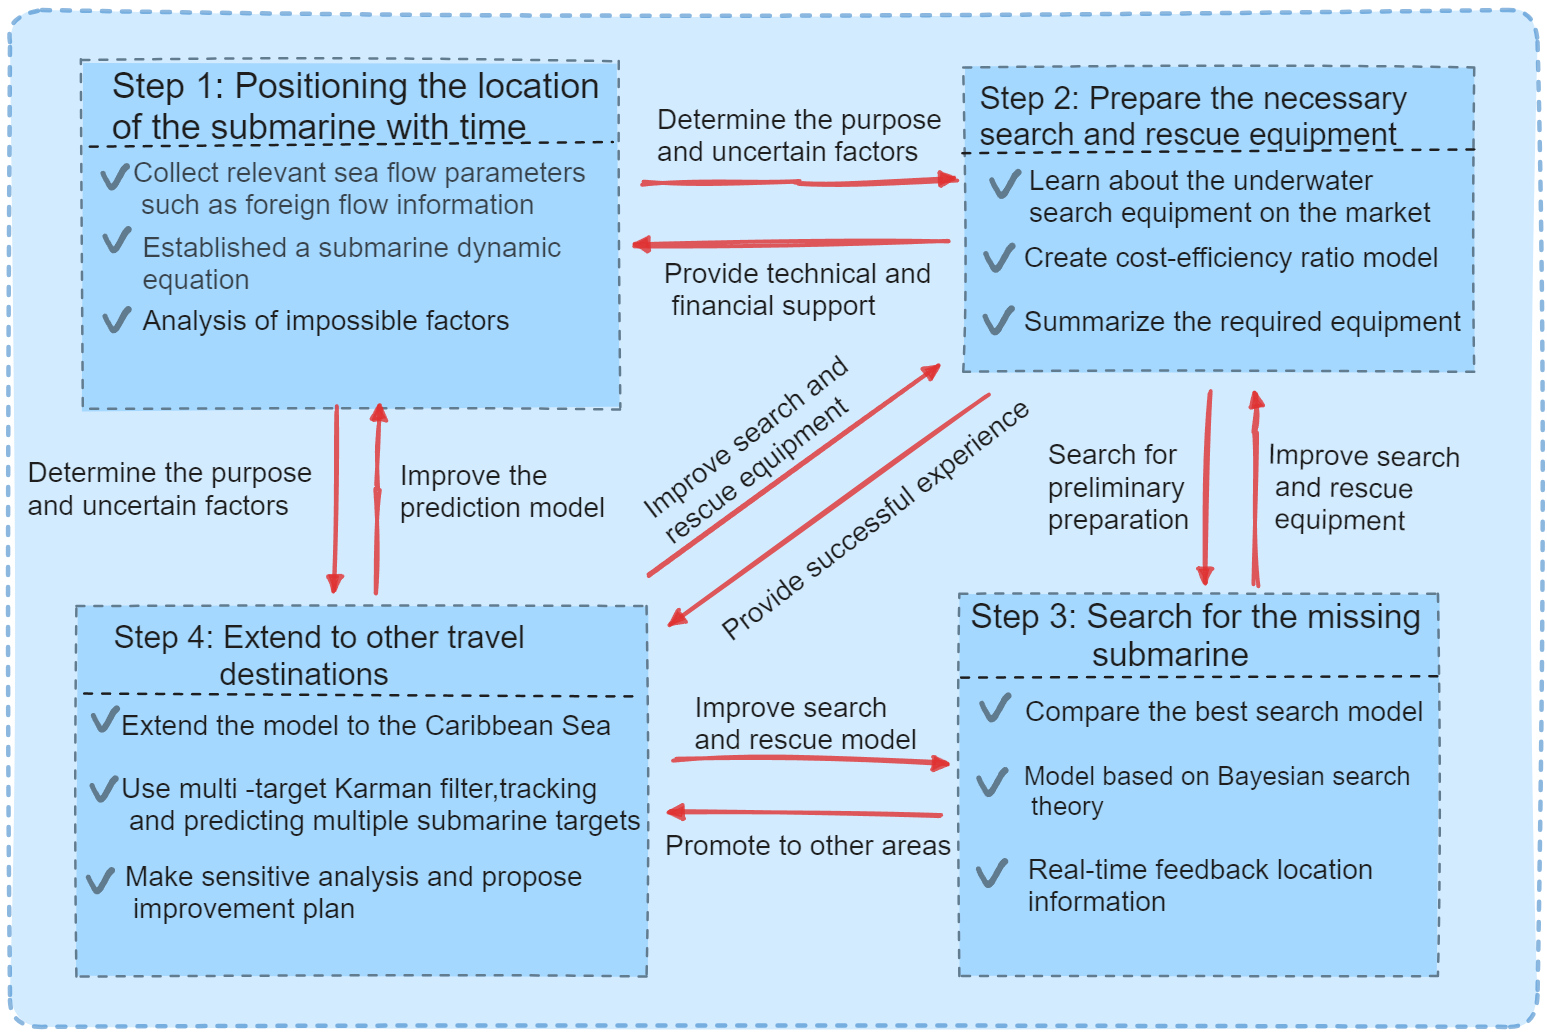
\includegraphics[width=453.55pt,height=303.75pt]{latexImage_78014f4da7fb4ed64d2aedb4cdecba75.png}}
\put(244.6,-378.611){\fontsize{11}{1}\usefont{T1}{cmr}{m}{n}\selectfont\color{color_80434}图}
\put(257.8,-378.611){\fontsize{11}{1}\usefont{T1}{ptm}{m}{n}\selectfont\color{color_80434}1}
\put(263.201,-378.611){\fontsize{11}{1}\usefont{T1}{ptm}{m}{n}\selectfont\color{color_80434}.}
\put(266,-378.611){\fontsize{11}{1}\usefont{T1}{cmr}{m}{n}\selectfont\color{color_80434}我}
\put(277,-378.611){\fontsize{11}{1}\usefont{T1}{cmr}{m}{n}\selectfont\color{color_80434}们的}
\put(299,-378.611){\fontsize{11}{1}\usefont{T1}{cmr}{m}{n}\selectfont\color{color_80434}工作}
\put(56,-400.911){\fontsize{18}{1}\usefont{T1}{cmr}{m}{n}\selectfont\color{color_55609}二、}
\put(98,-400.911){\fontsize{18}{1}\usefont{T1}{cmr}{m}{n}\selectfont\color{color_55609}假}
\put(116,-400.911){\fontsize{18}{1}\usefont{T1}{cmr}{m}{n}\selectfont\color{color_55609}设}
\put(56,-433.911){\fontsize{12}{1}\usefont{T1}{cmr}{m}{n}\selectfont\color{color_80434}为了简化问题,}
\put(140,-433.911){\fontsize{12}{1}\usefont{T1}{cmr}{m}{n}\selectfont\color{color_80434}我}
\put(152,-433.911){\fontsize{12}{1}\usefont{T1}{cmr}{m}{n}\selectfont\color{color_80434}们}
\put(164,-433.911){\fontsize{12}{1}\usefont{T1}{cmr}{m}{n}\selectfont\color{color_80434}做}
\put(176,-433.911){\fontsize{12}{1}\usefont{T1}{cmr}{m}{n}\selectfont\color{color_80434}了以下基本}
\put(236,-433.911){\fontsize{12}{1}\usefont{T1}{cmr}{m}{n}\selectfont\color{color_80434}假}
\put(248,-433.911){\fontsize{12}{1}\usefont{T1}{cmr}{m}{n}\selectfont\color{color_80434}设,}
\put(272,-433.911){\fontsize{12}{1}\usefont{T1}{cmr}{m}{n}\selectfont\color{color_80434}每}
\put(284,-433.911){\fontsize{12}{1}\usefont{T1}{cmr}{m}{n}\selectfont\color{color_80434}一个}
\put(308,-433.911){\fontsize{12}{1}\usefont{T1}{cmr}{m}{n}\selectfont\color{color_80434}假}
\put(320,-433.911){\fontsize{12}{1}\usefont{T1}{cmr}{m}{n}\selectfont\color{color_80434}设}
\put(332,-433.911){\fontsize{12}{1}\usefont{T1}{cmr}{m}{n}\selectfont\color{color_80434}都是}
\put(356,-433.911){\fontsize{12}{1}\usefont{T1}{cmr}{m}{n}\selectfont\color{color_80434}合理的}
\put(56,-454.211){\fontsize{12}{1}\usefont{T1}{cmr}{m}{n}\selectfont\color{color_29791}假}
\put(68,-454.211){\fontsize{12}{1}\usefont{T1}{cmr}{m}{n}\selectfont\color{color_29791}设一:}
\put(104,-454.211){\fontsize{12}{1}\usefont{T1}{cmr}{m}{n}\selectfont\color{color_29791}预}
\put(116,-454.211){\fontsize{12}{1}\usefont{T1}{cmr}{m}{n}\selectfont\color{color_29791}处}
\put(128,-454.211){\fontsize{12}{1}\usefont{T1}{cmr}{m}{n}\selectfont\color{color_29791}理数据}
\put(164,-454.211){\fontsize{12}{1}\usefont{T1}{cmr}{m}{n}\selectfont\color{color_29791}是}
\put(176,-454.211){\fontsize{12}{1}\usefont{T1}{cmr}{m}{n}\selectfont\color{color_29791}可}
\put(188,-454.211){\fontsize{12}{1}\usefont{T1}{cmr}{m}{n}\selectfont\color{color_29791}靠}
\put(200,-454.211){\fontsize{12}{1}\usefont{T1}{cmr}{m}{n}\selectfont\color{color_29791}的}
\put(56,-477.711){\fontsize{12}{1}\usefont{T1}{cmr}{m}{n}\selectfont\color{color_29791}理}
\put(68,-477.711){\fontsize{12}{1}\usefont{T1}{cmr}{m}{n}\selectfont\color{color_29791}由}
\put(80,-477.711){\fontsize{12}{1}\usefont{T1}{cmr}{m}{n}\selectfont\color{color_29791}:}
\put(92,-477.711){\fontsize{12}{1}\usefont{T1}{cmr}{m}{n}\selectfont\color{color_29791}这个}
\put(116,-477.711){\fontsize{12}{1}\usefont{T1}{cmr}{m}{n}\selectfont\color{color_29791}假}
\put(128,-477.711){\fontsize{12}{1}\usefont{T1}{cmr}{m}{n}\selectfont\color{color_29791}设}
\put(140,-477.711){\fontsize{12}{1}\usefont{T1}{cmr}{m}{n}\selectfont\color{color_29791}是}
\put(152,-477.711){\fontsize{12}{1}\usefont{T1}{cmr}{m}{n}\selectfont\color{color_29791}为了确}
\put(188,-477.711){\fontsize{12}{1}\usefont{T1}{cmr}{m}{n}\selectfont\color{color_29791}保}
\put(200,-477.711){\fontsize{12}{1}\usefont{T1}{cmr}{m}{n}\selectfont\color{color_29791}模型}
\put(224,-477.711){\fontsize{12}{1}\usefont{T1}{cmr}{m}{n}\selectfont\color{color_29791}解决}
\put(248,-477.711){\fontsize{12}{1}\usefont{T1}{cmr}{m}{n}\selectfont\color{color_29791}方案的准确性}
\put(56,-501.211){\fontsize{12}{1}\usefont{T1}{cmr}{m}{n}\selectfont\color{color_29791}假}
\put(68,-501.211){\fontsize{12}{1}\usefont{T1}{cmr}{m}{n}\selectfont\color{color_29791}设二:}
\put(104,-501.211){\fontsize{12}{1}\usefont{T1}{cmr}{m}{n}\selectfont\color{color_29791}没}
\put(116,-501.211){\fontsize{12}{1}\usefont{T1}{cmr}{m}{n}\selectfont\color{color_29791}有}
\put(128,-501.211){\fontsize{12}{1}\usefont{T1}{cmr}{m}{n}\selectfont\color{color_29791}其他特殊}
\put(176,-501.211){\fontsize{12}{1}\usefont{T1}{cmr}{m}{n}\selectfont\color{color_29791}情况,如}
\put(224,-501.211){\fontsize{12}{1}\usefont{T1}{cmr}{m}{n}\selectfont\color{color_29791}极端天}
\put(260,-501.211){\fontsize{12}{1}\usefont{T1}{cmr}{m}{n}\selectfont\color{color_29791}气}
\put(56,-524.711){\fontsize{12}{1}\usefont{T1}{cmr}{m}{n}\selectfont\color{color_29791}理}
\put(68,-524.711){\fontsize{12}{1}\usefont{T1}{cmr}{m}{n}\selectfont\color{color_29791}由}
\put(80,-524.711){\fontsize{12}{1}\usefont{T1}{cmr}{m}{n}\selectfont\color{color_29791}:}
\put(92,-524.711){\fontsize{12}{1}\usefont{T1}{cmr}{m}{n}\selectfont\color{color_29791}为了简化模型,本文}
\put(200,-524.711){\fontsize{12}{1}\usefont{T1}{cmr}{m}{n}\selectfont\color{color_29791}忽略}
\put(224,-524.711){\fontsize{12}{1}\usefont{T1}{cmr}{m}{n}\selectfont\color{color_29791}了}
\put(236,-524.711){\fontsize{12}{1}\usefont{T1}{cmr}{m}{n}\selectfont\color{color_29791}极端天}
\put(272,-524.711){\fontsize{12}{1}\usefont{T1}{cmr}{m}{n}\selectfont\color{color_29791}气对信息的}
\put(332,-524.711){\fontsize{12}{1}\usefont{T1}{cmr}{m}{n}\selectfont\color{color_29791}干扰}
\put(356,-524.711){\fontsize{12}{1}\usefont{T1}{ptm}{m}{n}\selectfont\color{color_29791};}
\put(359.3,-524.711){\fontsize{12}{1}\usefont{T1}{cmr}{m}{n}\selectfont\color{color_29791}事实}
\put(383.3,-524.711){\fontsize{12}{1}\usefont{T1}{cmr}{m}{n}\selectfont\color{color_29791}上,}
\put(407.3,-524.711){\fontsize{12}{1}\usefont{T1}{cmr}{m}{n}\selectfont\color{color_29791}极端天}
\put(443.3,-524.711){\fontsize{12}{1}\usefont{T1}{cmr}{m}{n}\selectfont\color{color_29791}气}
\put(455.3,-524.711){\fontsize{12}{1}\usefont{T1}{cmr}{m}{n}\selectfont\color{color_29791}会}
\put(467.3,-524.711){\fontsize{12}{1}\usefont{T1}{cmr}{m}{n}\selectfont\color{color_29791}对模型}
\put(56,-545.211){\fontsize{12}{1}\usefont{T1}{cmr}{m}{n}\selectfont\color{color_29791}产生很大}
\put(104,-545.211){\fontsize{12}{1}\usefont{T1}{cmr}{m}{n}\selectfont\color{color_29791}的}
\put(116,-545.211){\fontsize{12}{1}\usefont{T1}{cmr}{m}{n}\selectfont\color{color_29791}影响}
\put(140,-545.211){\fontsize{12}{1}\usefont{T1}{cmr}{m}{n}\selectfont\color{color_29791},}
\put(152,-545.211){\fontsize{12}{1}\usefont{T1}{cmr}{m}{n}\selectfont\color{color_29791}但}
\put(164,-545.211){\fontsize{12}{1}\usefont{T1}{cmr}{m}{n}\selectfont\color{color_29791}这}
\put(176,-545.211){\fontsize{12}{1}\usefont{T1}{cmr}{m}{n}\selectfont\color{color_29791}种}
\put(188,-545.211){\fontsize{12}{1}\usefont{T1}{cmr}{m}{n}\selectfont\color{color_29791}可能性}
\put(224,-545.211){\fontsize{12}{1}\usefont{T1}{cmr}{m}{n}\selectfont\color{color_29791}很小}
\put(248,-545.211){\fontsize{12}{1}\usefont{T1}{cmr}{m}{n}\selectfont\color{color_29791},现在可以}
\put(308,-545.211){\fontsize{12}{1}\usefont{T1}{cmr}{m}{n}\selectfont\color{color_29791}忽略}
\put(332,-545.211){\fontsize{12}{1}\usefont{T1}{cmr}{m}{n}\selectfont\color{color_29791}不计}
\put(356,-545.211){\fontsize{12}{1}\usefont{T1}{ptm}{m}{n}\selectfont\color{color_29791}.}
\put(56,-568.711){\fontsize{12}{1}\usefont{T1}{cmr}{m}{n}\selectfont\color{color_29791}假}
\put(68,-568.711){\fontsize{12}{1}\usefont{T1}{cmr}{m}{n}\selectfont\color{color_29791}设三:}
\put(104,-568.711){\fontsize{12}{1}\usefont{T1}{cmr}{m}{n}\selectfont\color{color_29791}爱奥尼亚海与加勒比海的海水}
\put(260,-568.711){\fontsize{12}{1}\usefont{T1}{cmr}{m}{n}\selectfont\color{color_29791}密度}
\put(284,-568.711){\fontsize{12}{1}\usefont{T1}{cmr}{m}{n}\selectfont\color{color_29791}为}
\put(298.4,-568.711){\fontsize{12}{1}\usefont{T1}{ptm}{b}{n}\selectfont\color{color_29791}1g/}
\put(313.7,-568.711){\fontsize{12}{1}\usefont{T1}{ptm}{b}{n}\selectfont\color{color_29791}c}
\put(319.004,-568.711){\fontsize{12}{1}\usefont{T1}{ptm}{b}{n}\selectfont\color{color_29791}m³.}
\put(56,-592.211){\fontsize{12}{1}\usefont{T1}{cmr}{m}{n}\selectfont\color{color_29791}理}
\put(68,-592.211){\fontsize{12}{1}\usefont{T1}{cmr}{m}{n}\selectfont\color{color_29791}由}
\put(80,-592.211){\fontsize{12}{1}\usefont{T1}{cmr}{m}{n}\selectfont\color{color_29791}:}
\put(92,-592.211){\fontsize{12}{1}\usefont{T1}{cmr}{m}{n}\selectfont\color{color_29791}由}
\put(104,-592.211){\fontsize{12}{1}\usefont{T1}{cmr}{m}{n}\selectfont\color{color_29791}于模型}
\put(140,-592.211){\fontsize{12}{1}\usefont{T1}{cmr}{m}{n}\selectfont\color{color_29791}涉}
\put(152,-592.211){\fontsize{12}{1}\usefont{T1}{cmr}{m}{n}\selectfont\color{color_29791}及的数据}
\put(200,-592.211){\fontsize{12}{1}\usefont{T1}{cmr}{m}{n}\selectfont\color{color_29791}量}
\put(212,-592.211){\fontsize{12}{1}\usefont{T1}{cmr}{m}{n}\selectfont\color{color_29791}较}
\put(224,-592.211){\fontsize{12}{1}\usefont{T1}{cmr}{m}{n}\selectfont\color{color_29791}大}
\put(236,-592.211){\fontsize{12}{1}\usefont{T1}{cmr}{m}{n}\selectfont\color{color_29791},海水的}
\put(284,-592.211){\fontsize{12}{1}\usefont{T1}{cmr}{m}{n}\selectfont\color{color_29791}密度非}
\put(320,-592.211){\fontsize{12}{1}\usefont{T1}{cmr}{m}{n}\selectfont\color{color_29791}常}
\put(332,-592.211){\fontsize{12}{1}\usefont{T1}{cmr}{m}{n}\selectfont\color{color_29791}接近}
\put(358.4,-592.211){\fontsize{12}{1}\usefont{T1}{ptm}{m}{n}\selectfont\color{color_29791}1g/}
\put(373.7,-592.211){\fontsize{12}{1}\usefont{T1}{ptm}{m}{n}\selectfont\color{color_29791}c}
\put(379.004,-592.211){\fontsize{12}{1}\usefont{T1}{ptm}{m}{n}\selectfont\color{color_29791}m}
\put(388.304,-592.211){\fontsize{12}{1}\usefont{T1}{ptm}{m}{n}\selectfont\color{color_29791}³}
\put(392,-592.211){\fontsize{12}{1}\usefont{T1}{cmr}{m}{n}\selectfont\color{color_29791},因此最}
\put(440,-592.211){\fontsize{12}{1}\usefont{T1}{cmr}{m}{n}\selectfont\color{color_29791}终误差}
\put(476,-592.211){\fontsize{12}{1}\usefont{T1}{cmr}{m}{n}\selectfont\color{color_29791}可以}
\put(56,-612.711){\fontsize{12}{1}\usefont{T1}{cmr}{m}{n}\selectfont\color{color_29791}忽略}
\put(80,-612.711){\fontsize{12}{1}\usefont{T1}{cmr}{m}{n}\selectfont\color{color_29791}不计}
\put(56,-636.211){\fontsize{12}{1}\usefont{T1}{cmr}{m}{n}\selectfont\color{color_29791}假}
\put(68,-636.211){\fontsize{12}{1}\usefont{T1}{cmr}{m}{n}\selectfont\color{color_29791}设}
\put(80,-636.211){\fontsize{12}{1}\usefont{T1}{cmr}{m}{n}\selectfont\color{color_29791}四}
\put(92,-636.211){\fontsize{12}{1}\usefont{T1}{cmr}{m}{n}\selectfont\color{color_29791}:}
\put(104,-636.211){\fontsize{12}{1}\usefont{T1}{cmr}{m}{n}\selectfont\color{color_29791}潜艇}
\put(128,-636.211){\fontsize{12}{1}\usefont{T1}{cmr}{m}{n}\selectfont\color{color_29791}故障}
\put(152,-636.211){\fontsize{12}{1}\usefont{T1}{cmr}{m}{n}\selectfont\color{color_29791}后}
\put(164,-636.211){\fontsize{12}{1}\usefont{T1}{cmr}{m}{n}\selectfont\color{color_29791}无}
\put(176,-636.211){\fontsize{12}{1}\usefont{T1}{cmr}{m}{n}\selectfont\color{color_29791}通信}
\put(200,-636.211){\fontsize{12}{1}\usefont{T1}{cmr}{m}{n}\selectfont\color{color_29791}功}
\put(212,-636.211){\fontsize{12}{1}\usefont{T1}{cmr}{m}{n}\selectfont\color{color_29791}能,且动力系}
\put(284,-636.211){\fontsize{12}{1}\usefont{T1}{cmr}{m}{n}\selectfont\color{color_29791}统无}
\put(308,-636.211){\fontsize{12}{1}\usefont{T1}{cmr}{m}{n}\selectfont\color{color_29791}法}
\put(320,-636.211){\fontsize{12}{1}\usefont{T1}{cmr}{m}{n}\selectfont\color{color_29791}正}
\put(332,-636.211){\fontsize{12}{1}\usefont{T1}{cmr}{m}{n}\selectfont\color{color_29791}常使用}
\put(56,-659.711){\fontsize{12}{1}\usefont{T1}{cmr}{m}{n}\selectfont\color{color_29791}理}
\put(68,-659.711){\fontsize{12}{1}\usefont{T1}{cmr}{m}{n}\selectfont\color{color_29791}由}
\put(80,-659.711){\fontsize{12}{1}\usefont{T1}{cmr}{m}{n}\selectfont\color{color_29791}:}
\put(92,-659.711){\fontsize{12}{1}\usefont{T1}{cmr}{m}{n}\selectfont\color{color_29791}简化模型,}
\put(152,-659.711){\fontsize{12}{1}\usefont{T1}{cmr}{m}{n}\selectfont\color{color_29791}便}
\put(164,-659.711){\fontsize{12}{1}\usefont{T1}{cmr}{m}{n}\selectfont\color{color_29791}于计算}
\put(56,-685.511){\fontsize{18}{1}\usefont{T1}{cmr}{m}{n}\selectfont\color{color_55609}三、}
\put(98,-685.511){\fontsize{18}{1}\usefont{T1}{cmr}{m}{n}\selectfont\color{color_55609}符号}
\put(134,-685.511){\fontsize{18}{1}\usefont{T1}{cmr}{m}{n}\selectfont\color{color_55609}和定}
\put(170,-685.511){\fontsize{18}{1}\usefont{T1}{cmr}{m}{n}\selectfont\color{color_55609}义}
\put(200.9,-721.811){\fontsize{12}{1}\usefont{T1}{ptm}{b}{n}\selectfont\color{color_29791}T}
\put(207.5,-721.811){\fontsize{12}{1}\usefont{T1}{ptm}{b}{n}\selectfont\color{color_29791}ab}
\put(224.18,-721.811){\fontsize{12}{1}\usefont{T1}{ptm}{b}{n}\selectfont\color{color_29791}l}
\put(228.368,-721.811){\fontsize{12}{1}\usefont{T1}{ptm}{b}{n}\selectfont\color{color_29791}e}
\put(236.468,-721.811){\fontsize{12}{1}\usefont{T1}{ptm}{b}{n}\selectfont\color{color_29791} }
\put(240.656,-721.811){\fontsize{12}{1}\usefont{T1}{ptm}{b}{n}\selectfont\color{color_29791}2}
\put(248.96,-721.811){\fontsize{12}{1}\usefont{T1}{ptm}{b}{n}\selectfont\color{color_29791}.}
\put(253.544,-721.811){\fontsize{12}{1}\usefont{T1}{ptm}{b}{n}\selectfont\color{color_29791} }
\put(257.732,-721.811){\fontsize{12}{1}\usefont{T1}{ptm}{b}{n}\selectfont\color{color_29791}M}
\put(269.636,-721.811){\fontsize{12}{1}\usefont{T1}{ptm}{b}{n}\selectfont\color{color_29791}ajo}
\put(290.024,-721.811){\fontsize{12}{1}\usefont{T1}{ptm}{b}{n}\selectfont\color{color_29791}r}
\put(296.012,-721.811){\fontsize{12}{1}\usefont{T1}{ptm}{b}{n}\selectfont\color{color_29791} }
\put(300.2,-721.811){\fontsize{12}{1}\usefont{T1}{ptm}{b}{n}\selectfont\color{color_29791}n}
\put(308.696,-721.811){\fontsize{12}{1}\usefont{T1}{ptm}{b}{n}\selectfont\color{color_29791}o}
\put(316.892,-721.811){\fontsize{12}{1}\usefont{T1}{ptm}{b}{n}\selectfont\color{color_29791}t}
\put(322.592,-721.811){\fontsize{12}{1}\usefont{T1}{ptm}{b}{n}\selectfont\color{color_29791}a}
\put(330.776,-721.811){\fontsize{12}{1}\usefont{T1}{ptm}{b}{n}\selectfont\color{color_29791}t}
\put(336.476,-721.811){\fontsize{12}{1}\usefont{T1}{ptm}{b}{n}\selectfont\color{color_29791}io}
\put(348.872,-721.811){\fontsize{12}{1}\usefont{T1}{ptm}{b}{n}\selectfont\color{color_29791}n}
\put(357.368,-721.811){\fontsize{12}{1}\usefont{T1}{ptm}{b}{n}\selectfont\color{color_29791}s}
\put(364.556,-721.811){\fontsize{12}{1}\usefont{T1}{ptm}{b}{n}\selectfont\color{color_29791} }
\end{picture}
\newpage
\begin{tikzpicture}[overlay]
\path(0pt,0pt);
\draw[color_231438,line width=0.75pt,line join=round]
(55.85pt, -62.01099pt) -- (507.1pt, -62.01099pt)
;
\draw[color_231438,line width=0.75pt,line join=round]
(55.85pt, -83.211pt) -- (507.1pt, -83.211pt)
;
\draw[color_231438,line width=0.75pt,line join=round]
(56.2pt, -61.61102pt) -- (56.2pt, -83.56097pt)
;
\draw[color_231438,line width=0.75pt,line join=round]
(281pt, -61.61102pt) -- (281pt, -83.56097pt)
;
\draw[color_231438,line width=0.75pt,line join=round]
(506.7pt, -61.61102pt) -- (506.7pt, -83.56097pt)
;
\end{tikzpicture}
\begin{picture}(-5,0)(2.5,0)
\put(146.2,-76.211){\fontsize{10.5}{1}\usefont{T1}{cmr}{m}{n}\selectfont\color{color_29791}N}
\put(154.0855,-76.211){\fontsize{10.5}{1}\usefont{T1}{cmr}{m}{n}\selectfont\color{color_29791}o}
\put(160.4905,-76.211){\fontsize{10.5}{1}\usefont{T1}{cmr}{m}{n}\selectfont\color{color_29791}t}
\put(164.5855,-76.211){\fontsize{10.5}{1}\usefont{T1}{cmr}{m}{n}\selectfont\color{color_29791}a}
\put(170.9905,-76.211){\fontsize{10.5}{1}\usefont{T1}{cmr}{m}{n}\selectfont\color{color_29791}t}
\put(175.0855,-76.211){\fontsize{10.5}{1}\usefont{T1}{cmr}{m}{n}\selectfont\color{color_29791}i}
\put(178.078,-76.211){\fontsize{10.5}{1}\usefont{T1}{cmr}{m}{n}\selectfont\color{color_29791}o}
\put(184.483,-76.211){\fontsize{10.5}{1}\usefont{T1}{cmr}{m}{n}\selectfont\color{color_29791}n}
\put(364.1,-76.211){\fontsize{10.5}{1}\usefont{T1}{cmr}{m}{n}\selectfont\color{color_29791}D}
\put(372.101,-76.211){\fontsize{10.5}{1}\usefont{T1}{cmr}{m}{n}\selectfont\color{color_29791}e}
\put(378.59,-76.211){\fontsize{10.5}{1}\usefont{T1}{cmr}{m}{n}\selectfont\color{color_29791}s}
\put(384.0815,-76.211){\fontsize{10.5}{1}\usefont{T1}{cmr}{m}{n}\selectfont\color{color_29791}c}
\put(389.867,-76.211){\fontsize{10.5}{1}\usefont{T1}{cmr}{m}{n}\selectfont\color{color_29791}r}
\put(394.172,-76.211){\fontsize{10.5}{1}\usefont{T1}{cmr}{m}{n}\selectfont\color{color_29791}i}
\put(397.07,-76.211){\fontsize{10.5}{1}\usefont{T1}{cmr}{m}{n}\selectfont\color{color_29791}p}
\put(403.7585,-76.211){\fontsize{10.5}{1}\usefont{T1}{cmr}{m}{n}\selectfont\color{color_29791}t}
\put(407.8535,-76.211){\fontsize{10.5}{1}\usefont{T1}{cmr}{m}{n}\selectfont\color{color_29791}i}
\put(410.7515,-76.211){\fontsize{10.5}{1}\usefont{T1}{cmr}{m}{n}\selectfont\color{color_29791}o}
\put(417.1565,-76.211){\fontsize{10.5}{1}\usefont{T1}{cmr}{m}{n}\selectfont\color{color_29791}n}
\end{picture}
\newpage
\begin{tikzpicture}[overlay]
\path(0pt,0pt);
\draw[color_231438,line width=0.75pt,line join=round]
(55.85pt, -62.01099pt) -- (507.1pt, -62.01099pt)
;
\draw[color_231438,line width=0.75pt,line join=round]
(55.85pt, -83.211pt) -- (507.1pt, -83.211pt)
;
\draw[color_231438,line width=0.75pt,line join=round]
(55.85pt, -104.511pt) -- (507.1pt, -104.511pt)
;
\draw[color_231438,line width=0.75pt,line join=round]
(55.85pt, -125.711pt) -- (507.1pt, -125.711pt)
;
\draw[color_231438,line width=0.75pt,line join=round]
(55.85pt, -147.011pt) -- (507.1pt, -147.011pt)
;
\draw[color_231438,line width=0.75pt,line join=round]
(55.85pt, -166.511pt) -- (507.1pt, -166.511pt)
;
\draw[color_231438,line width=0.75pt,line join=round]
(55.85pt, -187.311pt) -- (507.1pt, -187.311pt)
;
\draw[color_231438,line width=0.75pt,line join=round]
(55.85pt, -206.811pt) -- (507.1pt, -206.811pt)
;
\draw[color_231438,line width=0.75pt,line join=round]
(55.85pt, -227.711pt) -- (507.1pt, -227.711pt)
;
\draw[color_231438,line width=0.75pt,line join=round]
(55.85pt, -247.311pt) -- (507.1pt, -247.311pt)
;
\draw[color_231438,line width=0.75pt,line join=round]
(55.85pt, -270.511pt) -- (507.1pt, -270.511pt)
;
\draw[color_231438,line width=0.75pt,line join=round]
(55.85pt, -291.211pt) -- (507.1pt, -291.211pt)
;
\draw[color_231438,line width=0.75pt,line join=round]
(55.85pt, -312.011pt) -- (507.1pt, -312.011pt)
;
\draw[color_231438,line width=0.75pt,line join=round]
(55.85pt, -332.711pt) -- (507.1pt, -332.711pt)
;
\draw[color_231438,line width=0.75pt,line join=round]
(55.85pt, -353.011pt) -- (507.1pt, -353.011pt)
;
\draw[color_231438,line width=0.75pt,line join=round]
(55.85pt, -373.311pt) -- (507.1pt, -373.311pt)
;
\draw[color_231438,line width=0.75pt,line join=round]
(55.85pt, -393.611pt) -- (507.1pt, -393.611pt)
;
\draw[color_231438,line width=0.75pt,line join=round]
(55.85pt, -413.911pt) -- (507.1pt, -413.911pt)
;
\draw[color_231438,line width=0.75pt,line join=round]
(55.85pt, -434.211pt) -- (507.1pt, -434.211pt)
;
\draw[color_231438,line width=0.75pt,line join=round]
(55.85pt, -455.011pt) -- (507.1pt, -455.011pt)
;
\draw[color_231438,line width=0.75pt,line join=round]
(55.85pt, -475.711pt) -- (507.1pt, -475.711pt)
;
\draw[color_231438,line width=0.75pt,line join=round]
(55.85pt, -496.511pt) -- (507.1pt, -496.511pt)
;
\draw[color_231438,line width=0.75pt,line join=round]
(55.85pt, -517.211pt) -- (507.1pt, -517.211pt)
;
\draw[color_231438,line width=0.75pt,line join=round]
(55.85pt, -536.811pt) -- (507.1pt, -536.811pt)
;
\draw[color_231438,line width=0.75pt,line join=round]
(55.85pt, -556.411pt) -- (507.1pt, -556.411pt)
;
\draw[color_231438,line width=0.75pt,line join=round]
(55.85pt, -576.011pt) -- (507.1pt, -576.011pt)
;
\draw[color_231438,line width=0.75pt,line join=round]
(55.85pt, -595.511pt) -- (507.1pt, -595.511pt)
;
\draw[color_231438,line width=0.75pt,line join=round]
(55.85pt, -615.111pt) -- (507.1pt, -615.111pt)
;
\draw[color_231438,line width=0.75pt,line join=round]
(55.85pt, -634.711pt) -- (507.1pt, -634.711pt)
;
\draw[color_231438,line width=0.75pt,line join=round]
(55.85pt, -654.311pt) -- (507.1pt, -654.311pt)
;
\draw[color_231438,line width=0.75pt,line join=round]
(55.85pt, -673.911pt) -- (507.1pt, -673.911pt)
;
\draw[color_231438,line width=0.75pt,line join=round]
(55.85pt, -694.211pt) -- (507.1pt, -694.211pt)
;
\draw[color_231438,line width=0.75pt,line join=round]
(55.85pt, -714.511pt) -- (507.1pt, -714.511pt)
;
\draw[color_231438,line width=0.75pt,line join=round]
(55.85pt, -734.111pt) -- (507.1pt, -734.111pt)
;
\draw[color_231438,line width=0.75pt,line join=round]
(55.85pt, -753.711pt) -- (507.1pt, -753.711pt)
;
\draw[color_231438,line width=0.75pt,line join=round]
(56.2pt, -61.61102pt) -- (56.2pt, -754.061pt)
;
\draw[color_231438,line width=0.75pt,line join=round]
(281pt, -61.61102pt) -- (281pt, -754.061pt)
;
\draw[color_231438,line width=0.75pt,line join=round]
(506.7pt, -61.61102pt) -- (506.7pt, -754.061pt)
;
\end{tikzpicture}
\begin{picture}(-5,0)(2.5,0)
\put(350,-76.41101){\fontsize{11}{1}\usefont{T1}{cmr}{m}{n}\selectfont\color{color_80434}潜水器的位置向}
\put(427,-76.41101){\fontsize{11}{1}\usefont{T1}{cmr}{m}{n}\selectfont\color{color_80434}量}
\put(352,-97.41101){\fontsize{10.5}{1}\usefont{T1}{cmr}{m}{n}\selectfont\color{color_29791}潜水器}
\put(383.5,-97.41101){\fontsize{10.5}{1}\usefont{T1}{cmr}{m}{n}\selectfont\color{color_29791}运}
\put(394,-97.41101){\fontsize{10.5}{1}\usefont{T1}{cmr}{m}{n}\selectfont\color{color_29791}动的时间}
\put(362.5,-118.711){\fontsize{10.5}{1}\usefont{T1}{cmr}{m}{n}\selectfont\color{color_29791}潜水艇的}
\put(404.5,-118.711){\fontsize{10.5}{1}\usefont{T1}{cmr}{m}{n}\selectfont\color{color_29791}质量}
\put(366.5,-140.111){\fontsize{11}{1}\usefont{T1}{cmr}{m}{n}\selectfont\color{color_80434}重力加}
\put(399.5,-140.111){\fontsize{11}{1}\usefont{T1}{cmr}{m}{n}\selectfont\color{color_80434}速度}
\put(361,-160.511){\fontsize{11}{1}\usefont{T1}{cmr}{m}{n}\selectfont\color{color_80434}潜水艇的重力}
\end{picture}
\begin{tikzpicture}[overlay]
\path(0pt,0pt);
\filldraw[color_283006][even odd rule]
(333.9pt, -183.861pt) -- (453.85pt, -183.861pt)
 -- (453.85pt, -183.861pt)
 -- (453.85pt, -169.911pt)
 -- (453.85pt, -169.911pt)
 -- (333.9pt, -169.911pt) -- cycle
;
\end{tikzpicture}
\begin{picture}(-5,0)(2.5,0)
\put(334,-181.011){\fontsize{12}{1}\usefont{T1}{cmr}{m}{n}\selectfont\color{color_54684}水流对潜水器的}
\put(418,-181.011){\fontsize{12}{1}\usefont{T1}{cmr}{m}{n}\selectfont\color{color_54684}作}
\put(430,-181.011){\fontsize{12}{1}\usefont{T1}{cmr}{m}{n}\selectfont\color{color_54684}用力}
\put(355.5,-200.811){\fontsize{11}{1}\usefont{T1}{cmr}{m}{n}\selectfont\color{color_80434}潜水艇}
\put(388.5,-200.811){\fontsize{11}{1}\usefont{T1}{cmr}{m}{n}\selectfont\color{color_80434}所}
\put(399.5,-200.811){\fontsize{11}{1}\usefont{T1}{cmr}{m}{n}\selectfont\color{color_80434}受}
\put(410.5,-200.811){\fontsize{11}{1}\usefont{T1}{cmr}{m}{n}\selectfont\color{color_80434}浮}
\put(421.5,-200.811){\fontsize{11}{1}\usefont{T1}{cmr}{m}{n}\selectfont\color{color_80434}力}
\end{picture}
\begin{tikzpicture}[overlay]
\path(0pt,0pt);
\filldraw[color_283006][even odd rule]
(174.7pt, -224.261pt) -- (176.85pt, -224.261pt)
 -- (176.85pt, -224.261pt)
 -- (176.85pt, -210.311pt)
 -- (176.85pt, -210.311pt)
 -- (174.7pt, -210.311pt) -- cycle
;
\end{tikzpicture}
\begin{picture}(-5,0)(2.5,0)
\put(174.8,-222.611){\fontsize{7}{1}\usefont{T1}{cmr}{m}{n}\selectfont\color{color_54684} }
\put(355.5,-221.011){\fontsize{11}{1}\usefont{T1}{cmr}{m}{n}\selectfont\color{color_80434}潜水艇}
\put(388.5,-221.011){\fontsize{11}{1}\usefont{T1}{cmr}{m}{n}\selectfont\color{color_80434}所}
\put(399.5,-221.011){\fontsize{11}{1}\usefont{T1}{cmr}{m}{n}\selectfont\color{color_80434}受}
\put(410.5,-221.011){\fontsize{11}{1}\usefont{T1}{cmr}{m}{n}\selectfont\color{color_80434}阻}
\put(421.5,-221.011){\fontsize{11}{1}\usefont{T1}{cmr}{m}{n}\selectfont\color{color_80434}力}
\put(366.5,-241.311){\fontsize{11}{1}\usefont{T1}{cmr}{m}{n}\selectfont\color{color_80434}海水的}
\put(399.5,-241.311){\fontsize{11}{1}\usefont{T1}{cmr}{m}{n}\selectfont\color{color_80434}密度}
\end{picture}
\begin{tikzpicture}[overlay]
\path(0pt,0pt);
\filldraw[color_283006][even odd rule]
(333.9pt, -265.761pt) -- (453.85pt, -265.761pt)
 -- (453.85pt, -265.761pt)
 -- (453.85pt, -251.811pt)
 -- (453.85pt, -251.811pt)
 -- (333.9pt, -251.811pt) -- cycle
;
\end{tikzpicture}
\begin{picture}(-5,0)(2.5,0)
\put(334,-263.011){\fontsize{12}{1}\usefont{T1}{cmr}{m}{n}\selectfont\color{color_54684}潜水器相对于水的}
\put(430,-263.011){\fontsize{12}{1}\usefont{T1}{cmr}{m}{n}\selectfont\color{color_54684}速度}
\end{picture}
\begin{tikzpicture}[overlay]
\path(0pt,0pt);
\filldraw[color_283006][even odd rule]
(369.9pt, -287.761pt) -- (417.85pt, -287.761pt)
 -- (417.85pt, -287.761pt)
 -- (417.85pt, -273.811pt)
 -- (417.85pt, -273.811pt)
 -- (369.9pt, -273.811pt) -- cycle
;
\end{tikzpicture}
\begin{picture}(-5,0)(2.5,0)
\put(370,-285.011){\fontsize{12}{1}\usefont{T1}{cmr}{m}{n}\selectfont\color{color_54684}阻}
\put(382,-285.011){\fontsize{12}{1}\usefont{T1}{cmr}{m}{n}\selectfont\color{color_54684}力系数}
\end{picture}
\begin{tikzpicture}[overlay]
\path(0pt,0pt);
\filldraw[color_283006][even odd rule]
(351.9pt, -308.561pt) -- (435.85pt, -308.561pt)
 -- (435.85pt, -308.561pt)
 -- (435.85pt, -294.611pt)
 -- (435.85pt, -294.611pt)
 -- (351.9pt, -294.611pt) -- cycle
;
\end{tikzpicture}
\begin{picture}(-5,0)(2.5,0)
\put(352,-305.711){\fontsize{12}{1}\usefont{T1}{cmr}{m}{n}\selectfont\color{color_54684}潜水器}
\put(388,-305.711){\fontsize{12}{1}\usefont{T1}{cmr}{m}{n}\selectfont\color{color_54684}迎}
\put(400,-305.711){\fontsize{12}{1}\usefont{T1}{cmr}{m}{n}\selectfont\color{color_54684}水面}
\put(424,-305.711){\fontsize{12}{1}\usefont{T1}{cmr}{m}{n}\selectfont\color{color_54684}积}
\put(418,-326.511){\fontsize{12}{1}\usefont{T1}{cmr}{m}{n}\selectfont\color{color_84742} }
\put(370,-326.511){\fontsize{12}{1}\usefont{T1}{cmr}{m}{n}\selectfont\color{color_84742}时间间}
\put(406,-326.511){\fontsize{12}{1}\usefont{T1}{cmr}{m}{n}\selectfont\color{color_84742}隔}
\put(382.7,-346.611){\fontsize{11}{1}\usefont{T1}{cmr}{m}{n}\selectfont\color{color_84742} }
\put(338.7,-346.611){\fontsize{11}{1}\usefont{T1}{cmr}{m}{n}\selectfont\color{color_84742}时间}
\put(360.7,-346.611){\fontsize{11}{1}\usefont{T1}{cmr}{m}{n}\selectfont\color{color_84742}步长}
\put(390.7,-346.611){\fontsize{11}{1}\usefont{T1}{cmr}{m}{n}\selectfont\color{color_84742} }
\put(394.2,-346.611){\fontsize{11}{1}\usefont{T1}{cmr}{m}{n}\selectfont\color{color_84742}时}
\put(405.2,-346.611){\fontsize{11}{1}\usefont{T1}{cmr}{m}{n}\selectfont\color{color_84742}刻}
\put(416.2,-346.611){\fontsize{11}{1}\usefont{T1}{cmr}{m}{n}\selectfont\color{color_84742}的}
\put(427.2,-346.611){\fontsize{11}{1}\usefont{T1}{cmr}{m}{n}\selectfont\color{color_84742}速度}
\put(382.7,-366.911){\fontsize{11}{1}\usefont{T1}{cmr}{m}{n}\selectfont\color{color_84742} }
\put(338.7,-366.911){\fontsize{11}{1}\usefont{T1}{cmr}{m}{n}\selectfont\color{color_84742}时间}
\put(360.7,-366.911){\fontsize{11}{1}\usefont{T1}{cmr}{m}{n}\selectfont\color{color_84742}步长}
\put(390.7,-366.911){\fontsize{11}{1}\usefont{T1}{cmr}{m}{n}\selectfont\color{color_84742} }
\put(394.2,-366.911){\fontsize{11}{1}\usefont{T1}{cmr}{m}{n}\selectfont\color{color_84742}时}
\put(405.2,-366.911){\fontsize{11}{1}\usefont{T1}{cmr}{m}{n}\selectfont\color{color_84742}刻}
\put(416.2,-366.911){\fontsize{11}{1}\usefont{T1}{cmr}{m}{n}\selectfont\color{color_84742}的}
\put(427.2,-366.911){\fontsize{11}{1}\usefont{T1}{cmr}{m}{n}\selectfont\color{color_84742}浮}
\put(438.2,-366.911){\fontsize{11}{1}\usefont{T1}{cmr}{m}{n}\selectfont\color{color_84742}力}
\put(380.9,-387.211){\fontsize{11}{1}\usefont{T1}{cmr}{m}{n}\selectfont\color{color_84742}  }
\put(336.9,-387.211){\fontsize{11}{1}\usefont{T1}{cmr}{m}{n}\selectfont\color{color_84742}时间}
\put(358.9,-387.211){\fontsize{11}{1}\usefont{T1}{cmr}{m}{n}\selectfont\color{color_84742}步长}
\put(392.5,-387.211){\fontsize{11}{1}\usefont{T1}{cmr}{m}{n}\selectfont\color{color_84742} }
\put(396,-387.211){\fontsize{11}{1}\usefont{T1}{cmr}{m}{n}\selectfont\color{color_84742}时}
\put(407,-387.211){\fontsize{11}{1}\usefont{T1}{cmr}{m}{n}\selectfont\color{color_84742}刻}
\put(418,-387.211){\fontsize{11}{1}\usefont{T1}{cmr}{m}{n}\selectfont\color{color_84742}的重力}
\put(344.2,-407.511){\fontsize{11}{1}\usefont{T1}{cmr}{m}{n}\selectfont\color{color_84742} }
\put(300.2,-407.511){\fontsize{11}{1}\usefont{T1}{cmr}{m}{n}\selectfont\color{color_84742}时间}
\put(322.2,-407.511){\fontsize{11}{1}\usefont{T1}{cmr}{m}{n}\selectfont\color{color_84742}步长}
\put(352.2,-407.511){\fontsize{11}{1}\usefont{T1}{cmr}{m}{n}\selectfont\color{color_84742} }
\put(355.7,-407.511){\fontsize{11}{1}\usefont{T1}{cmr}{m}{n}\selectfont\color{color_84742}时}
\put(366.7,-407.511){\fontsize{11}{1}\usefont{T1}{cmr}{m}{n}\selectfont\color{color_84742}刻}
\put(377.7,-407.511){\fontsize{11}{1}\usefont{T1}{cmr}{m}{n}\selectfont\color{color_84742}水流对潜水器的}
\put(454.7,-407.511){\fontsize{11}{1}\usefont{T1}{cmr}{m}{n}\selectfont\color{color_84742}作}
\put(465.7,-407.511){\fontsize{11}{1}\usefont{T1}{cmr}{m}{n}\selectfont\color{color_84742}用力}
\put(382.7,-427.811){\fontsize{11}{1}\usefont{T1}{cmr}{m}{n}\selectfont\color{color_84742} }
\put(338.7,-427.811){\fontsize{11}{1}\usefont{T1}{cmr}{m}{n}\selectfont\color{color_84742}时间}
\put(360.7,-427.811){\fontsize{11}{1}\usefont{T1}{cmr}{m}{n}\selectfont\color{color_84742}步长}
\put(390.7,-427.811){\fontsize{11}{1}\usefont{T1}{cmr}{m}{n}\selectfont\color{color_84742} }
\put(394.2,-427.811){\fontsize{11}{1}\usefont{T1}{cmr}{m}{n}\selectfont\color{color_84742}时}
\put(405.2,-427.811){\fontsize{11}{1}\usefont{T1}{cmr}{m}{n}\selectfont\color{color_84742}刻}
\put(416.2,-427.811){\fontsize{11}{1}\usefont{T1}{cmr}{m}{n}\selectfont\color{color_84742}的}
\put(427.2,-427.811){\fontsize{11}{1}\usefont{T1}{cmr}{m}{n}\selectfont\color{color_84742}阻}
\put(438.2,-427.811){\fontsize{11}{1}\usefont{T1}{cmr}{m}{n}\selectfont\color{color_84742}力}
\put(369.9,-448.711){\fontsize{12}{1}\usefont{T1}{cmr}{m}{n}\selectfont\color{color_84742} }
\put(321.9,-448.711){\fontsize{12}{1}\usefont{T1}{cmr}{m}{n}\selectfont\color{color_84742}时间}
\put(345.9,-448.711){\fontsize{12}{1}\usefont{T1}{cmr}{m}{n}\selectfont\color{color_84742}步长}
\put(378.2,-448.711){\fontsize{12}{1}\usefont{T1}{cmr}{m}{n}\selectfont\color{color_84742} }
\put(382,-448.711){\fontsize{12}{1}\usefont{T1}{cmr}{m}{n}\selectfont\color{color_84742}时}
\put(394,-448.711){\fontsize{12}{1}\usefont{T1}{cmr}{m}{n}\selectfont\color{color_84742}刻}
\put(406,-448.711){\fontsize{12}{1}\usefont{T1}{cmr}{m}{n}\selectfont\color{color_84742}的}
\put(418,-448.711){\fontsize{12}{1}\usefont{T1}{cmr}{m}{n}\selectfont\color{color_84742}状}
\put(430,-448.711){\fontsize{12}{1}\usefont{T1}{cmr}{m}{n}\selectfont\color{color_84742}态向}
\put(454,-448.711){\fontsize{12}{1}\usefont{T1}{cmr}{m}{n}\selectfont\color{color_84742}量}
\put(358,-469.511){\fontsize{12}{1}\usefont{T1}{cmr}{m}{n}\selectfont\color{color_80434}状}
\put(370,-469.511){\fontsize{12}{1}\usefont{T1}{cmr}{m}{n}\selectfont\color{color_80434}态}
\put(382,-469.511){\fontsize{12}{1}\usefont{T1}{cmr}{m}{n}\selectfont\color{color_80434}转移矩阵}
\put(358,-490.211){\fontsize{12}{1}\usefont{T1}{cmr}{m}{n}\selectfont\color{color_80434}输入控}
\put(394,-490.211){\fontsize{12}{1}\usefont{T1}{cmr}{m}{n}\selectfont\color{color_80434}制}
\put(406,-490.211){\fontsize{12}{1}\usefont{T1}{cmr}{m}{n}\selectfont\color{color_80434}矩阵}
\put(325.7,-511.011){\fontsize{12}{1}\usefont{T1}{cmr}{m}{n}\selectfont\color{color_80434}时间}
\put(349.7,-511.011){\fontsize{12}{1}\usefont{T1}{cmr}{m}{n}\selectfont\color{color_80434}步长}
\put(378.2,-511.011){\fontsize{12}{1}\usefont{T1}{cmr}{m}{n}\selectfont\color{color_80434}时}
\put(390.2,-511.011){\fontsize{12}{1}\usefont{T1}{cmr}{m}{n}\selectfont\color{color_80434}刻}
\put(402.2,-511.011){\fontsize{12}{1}\usefont{T1}{cmr}{m}{n}\selectfont\color{color_80434}的}
\put(414.2,-511.011){\fontsize{12}{1}\usefont{T1}{cmr}{m}{n}\selectfont\color{color_80434}输入}
\put(438.2,-511.011){\fontsize{12}{1}\usefont{T1}{cmr}{m}{n}\selectfont\color{color_80434}向}
\put(450.2,-511.011){\fontsize{12}{1}\usefont{T1}{cmr}{m}{n}\selectfont\color{color_80434}量}
\put(357.1,-530.811){\fontsize{11}{1}\usefont{T1}{ptm}{m}{n}\selectfont\color{color_80434}k}
\put(364.8,-530.811){\fontsize{11}{1}\usefont{T1}{cmr}{m}{n}\selectfont\color{color_80434}时}
\put(375.8,-530.811){\fontsize{11}{1}\usefont{T1}{cmr}{m}{n}\selectfont\color{color_80434}刻状}
\put(397.8,-530.811){\fontsize{11}{1}\usefont{T1}{cmr}{m}{n}\selectfont\color{color_80434}态变}
\put(419.8,-530.811){\fontsize{11}{1}\usefont{T1}{cmr}{m}{n}\selectfont\color{color_80434}量}
\put(361,-550.411){\fontsize{11}{1}\usefont{T1}{cmr}{m}{n}\selectfont\color{color_80434}状}
\put(372,-550.411){\fontsize{11}{1}\usefont{T1}{cmr}{m}{n}\selectfont\color{color_80434}态}
\put(383,-550.411){\fontsize{11}{1}\usefont{T1}{cmr}{m}{n}\selectfont\color{color_80434}转移矩阵}
\put(362.6,-570.011){\fontsize{11}{1}\usefont{T1}{ptm}{m}{n}\selectfont\color{color_80434}k}
\put(370.3,-570.011){\fontsize{11}{1}\usefont{T1}{cmr}{m}{n}\selectfont\color{color_80434}时}
\put(381.3,-570.011){\fontsize{11}{1}\usefont{T1}{cmr}{m}{n}\selectfont\color{color_80434}刻}
\put(392.3,-570.011){\fontsize{11}{1}\usefont{T1}{cmr}{m}{n}\selectfont\color{color_80434}观测}
\put(414.3,-570.011){\fontsize{11}{1}\usefont{T1}{cmr}{m}{n}\selectfont\color{color_80434}值}
\put(372,-589.511){\fontsize{11}{1}\usefont{T1}{cmr}{m}{n}\selectfont\color{color_80434}观测}
\put(394,-589.511){\fontsize{11}{1}\usefont{T1}{cmr}{m}{n}\selectfont\color{color_80434}矩阵}
\put(357.1,-609.111){\fontsize{11}{1}\usefont{T1}{ptm}{m}{n}\selectfont\color{color_80434}k}
\put(364.8,-609.111){\fontsize{11}{1}\usefont{T1}{cmr}{m}{n}\selectfont\color{color_80434}时}
\put(375.8,-609.111){\fontsize{11}{1}\usefont{T1}{cmr}{m}{n}\selectfont\color{color_80434}刻}
\put(386.8,-609.111){\fontsize{11}{1}\usefont{T1}{cmr}{m}{n}\selectfont\color{color_80434}过程}
\put(408.8,-609.111){\fontsize{11}{1}\usefont{T1}{cmr}{m}{n}\selectfont\color{color_80434}噪}
\put(419.8,-609.111){\fontsize{11}{1}\usefont{T1}{cmr}{m}{n}\selectfont\color{color_80434}声}
\put(357.1,-628.711){\fontsize{11}{1}\usefont{T1}{ptm}{m}{n}\selectfont\color{color_80434}k}
\put(364.8,-628.711){\fontsize{11}{1}\usefont{T1}{cmr}{m}{n}\selectfont\color{color_80434}时}
\put(375.8,-628.711){\fontsize{11}{1}\usefont{T1}{cmr}{m}{n}\selectfont\color{color_80434}刻}
\put(386.8,-628.711){\fontsize{11}{1}\usefont{T1}{cmr}{m}{n}\selectfont\color{color_80434}观测}
\put(408.8,-628.711){\fontsize{11}{1}\usefont{T1}{cmr}{m}{n}\selectfont\color{color_80434}噪}
\put(419.8,-628.711){\fontsize{11}{1}\usefont{T1}{cmr}{m}{n}\selectfont\color{color_80434}声}
\put(364.4,-648.311){\fontsize{11}{1}\usefont{T1}{ptm}{m}{n}\selectfont\color{color_80434}K}
\put(372.298,-648.311){\fontsize{11}{1}\usefont{T1}{ptm}{m}{n}\selectfont\color{color_80434}a}
\put(377.182,-648.311){\fontsize{11}{1}\usefont{T1}{ptm}{m}{n}\selectfont\color{color_80434}l}
\put(380.273,-648.311){\fontsize{11}{1}\usefont{T1}{ptm}{m}{n}\selectfont\color{color_80434}m}
\put(388.864,-648.311){\fontsize{11}{1}\usefont{T1}{ptm}{m}{n}\selectfont\color{color_80434}a}
\put(393.748,-648.311){\fontsize{11}{1}\usefont{T1}{ptm}{m}{n}\selectfont\color{color_80434}n}
\put(401.5,-648.311){\fontsize{11}{1}\usefont{T1}{cmr}{m}{n}\selectfont\color{color_80434}增}
\put(412.5,-648.311){\fontsize{11}{1}\usefont{T1}{cmr}{m}{n}\selectfont\color{color_80434}益}
\put(372,-667.911){\fontsize{11}{1}\usefont{T1}{cmr}{m}{n}\selectfont\color{color_80434}设备成本}
\put(361,-687.811){\fontsize{11}{1}\usefont{T1}{cmr}{m}{n}\selectfont\color{color_80434}人员培训}
\put(405,-687.811){\fontsize{11}{1}\usefont{T1}{cmr}{m}{n}\selectfont\color{color_80434}成本}
\put(355.5,-708.111){\fontsize{11}{1}\usefont{T1}{cmr}{m}{n}\selectfont\color{color_80434}储}
\put(366.5,-708.111){\fontsize{11}{1}\usefont{T1}{cmr}{m}{n}\selectfont\color{color_80434}存和}
\put(388.5,-708.111){\fontsize{11}{1}\usefont{T1}{cmr}{m}{n}\selectfont\color{color_80434}保养}
\put(410.5,-708.111){\fontsize{11}{1}\usefont{T1}{cmr}{m}{n}\selectfont\color{color_80434}成本}
\put(336.6,-728.111){\fontsize{11}{1}\usefont{T1}{ptm}{m}{n}\selectfont\color{color_80434}K}
\put(344.498,-728.111){\fontsize{11}{1}\usefont{T1}{ptm}{m}{n}\selectfont\color{color_80434}l}
\put(347.589,-728.111){\fontsize{11}{1}\usefont{T1}{ptm}{m}{n}\selectfont\color{color_80434}e}
\put(352.473,-728.111){\fontsize{11}{1}\usefont{T1}{ptm}{m}{n}\selectfont\color{color_80434}i}
\put(355.564,-728.111){\fontsize{11}{1}\usefont{T1}{ptm}{m}{n}\selectfont\color{color_80434}n4000}
\put(451.3,-728.111){\fontsize{11}{1}\usefont{T1}{cmr}{m}{n}\selectfont\color{color_80434}  }
\put(385.3,-728.111){\fontsize{11}{1}\usefont{T1}{cmr}{m}{n}\selectfont\color{color_80434}侧扫声纳个数}
\put(177,-748.811){\fontsize{11}{1}\usefont{T1}{ptm}{m}{n}\selectfont\color{color_80434} }
\put(313.6,-747.711){\fontsize{11}{1}\usefont{T1}{ptm}{m}{n}\selectfont\color{color_80434}M}
\put(323.39,-747.711){\fontsize{11}{1}\usefont{T1}{ptm}{m}{n}\selectfont\color{color_80434}E}
\put(330.089,-747.711){\fontsize{11}{1}\usefont{T1}{ptm}{m}{n}\selectfont\color{color_80434}P}
\put(336.194,-747.711){\fontsize{11}{1}\usefont{T1}{ptm}{m}{n}\selectfont\color{color_80434}U}
\put(344.092,-747.711){\fontsize{11}{1}\usefont{T1}{ptm}{m}{n}\selectfont\color{color_80434}S}
\put(350.1971,-747.711){\fontsize{11}{1}\usefont{T1}{ptm}{m}{n}\selectfont\color{color_80434}-}
\put(353.882,-747.711){\fontsize{11}{1}\usefont{T1}{ptm}{m}{n}\selectfont\color{color_80434}A}
\put(361.868,-747.711){\fontsize{11}{1}\usefont{T1}{ptm}{m}{n}\selectfont\color{color_80434}U}
\put(369.7661,-747.711){\fontsize{11}{1}\usefont{T1}{ptm}{m}{n}\selectfont\color{color_80434}V}
\put(377.6641,-747.711){\fontsize{11}{1}\usefont{T1}{ptm}{m}{n}\selectfont\color{color_80434}3000L}
\put(406.5,-747.711){\fontsize{11}{1}\usefont{T1}{cmr}{m}{n}\selectfont\color{color_80434}(}
\put(417.5,-747.711){\fontsize{11}{1}\usefont{T1}{ptm}{m}{n}\selectfont\color{color_80434}A}
\put(425.398,-747.711){\fontsize{11}{1}\usefont{T1}{ptm}{m}{n}\selectfont\color{color_80434}U}
\put(433.384,-747.711){\fontsize{11}{1}\usefont{T1}{ptm}{m}{n}\selectfont\color{color_80434}V}
\put(474.3,-747.711){\fontsize{11}{1}\usefont{T1}{cmr}{m}{n}\selectfont\color{color_80434} }
\put(441.3,-747.711){\fontsize{11}{1}\usefont{T1}{cmr}{m}{n}\selectfont\color{color_80434})个数}
\end{picture}
\newpage
\begin{tikzpicture}[overlay]
\path(0pt,0pt);
\draw[color_231438,line width=0.75pt,line join=round]
(55.85pt, -62.01099pt) -- (507.1pt, -62.01099pt)
;
\draw[color_231438,line width=0.75pt,line join=round]
(55.85pt, -81.61102pt) -- (507.1pt, -81.61102pt)
;
\draw[color_231438,line width=0.75pt,line join=round]
(55.85pt, -101.911pt) -- (507.1pt, -101.911pt)
;
\draw[color_231438,line width=0.75pt,line join=round]
(55.85pt, -121.411pt) -- (507.1pt, -121.411pt)
;
\draw[color_231438,line width=0.75pt,line join=round]
(55.85pt, -141.711pt) -- (507.1pt, -141.711pt)
;
\draw[color_231438,line width=0.75pt,line join=round]
(55.85pt, -161.911pt) -- (507.1pt, -161.911pt)
;
\draw[color_231438,line width=0.75pt,line join=round]
(55.85pt, -182.011pt) -- (507.1pt, -182.011pt)
;
\draw[color_231438,line width=0.75pt,line join=round]
(55.85pt, -202.211pt) -- (507.1pt, -202.211pt)
;
\draw[color_231438,line width=0.75pt,line join=round]
(55.85pt, -221.711pt) -- (507.1pt, -221.711pt)
;
\draw[color_231438,line width=0.75pt,line join=round]
(55.85pt, -241.911pt) -- (507.1pt, -241.911pt)
;
\draw[color_231438,line width=0.75pt,line join=round]
(55.85pt, -262.011pt) -- (507.1pt, -262.011pt)
;
\draw[color_231438,line width=0.75pt,line join=round]
(55.85pt, -289.311pt) -- (507.1pt, -289.311pt)
;
\draw[color_231438,line width=0.75pt,line join=round]
(55.85pt, -309.611pt) -- (507.1pt, -309.611pt)
;
\draw[color_231438,line width=0.75pt,line join=round]
(55.85pt, -329.911pt) -- (507.1pt, -329.911pt)
;
\draw[color_231438,line width=0.75pt,line join=round]
(55.85pt, -357.111pt) -- (507.1pt, -357.111pt)
;
\draw[color_231438,line width=0.75pt,line join=round]
(55.85pt, -377.411pt) -- (507.1pt, -377.411pt)
;
\draw[color_231438,line width=0.75pt,line join=round]
(55.85pt, -397.711pt) -- (507.1pt, -397.711pt)
;
\draw[color_231438,line width=0.75pt,line join=round]
(55.85pt, -418.011pt) -- (507.1pt, -418.011pt)
;
\draw[color_231438,line width=0.75pt,line join=round]
(55.85pt, -438.311pt) -- (507.1pt, -438.311pt)
;
\draw[color_231438,line width=0.75pt,line join=round]
(55.85pt, -458.611pt) -- (507.1pt, -458.611pt)
;
\draw[color_231438,line width=0.75pt,line join=round]
(55.85pt, -478.211pt) -- (507.1pt, -478.211pt)
;
\draw[color_231438,line width=0.75pt,line join=round]
(55.85pt, -497.711pt) -- (507.1pt, -497.711pt)
;
\draw[color_231438,line width=0.75pt,line join=round]
(55.85pt, -517.311pt) -- (507.1pt, -517.311pt)
;
\draw[color_231438,line width=0.75pt,line join=round]
(55.85pt, -536.811pt) -- (507.1pt, -536.811pt)
;
\draw[color_231438,line width=0.75pt,line join=round]
(55.85pt, -556.411pt) -- (507.1pt, -556.411pt)
;
\draw[color_231438,line width=0.75pt,line join=round]
(55.85pt, -575.911pt) -- (507.1pt, -575.911pt)
;
\draw[color_231438,line width=0.75pt,line join=round]
(55.85pt, -595.511pt) -- (507.1pt, -595.511pt)
;
\draw[color_231438,line width=0.75pt,line join=round]
(55.85pt, -615.011pt) -- (507.1pt, -615.011pt)
;
\draw[color_231438,line width=0.75pt,line join=round]
(55.85pt, -634.711pt) -- (507.1pt, -634.711pt)
;
\draw[color_231438,line width=0.75pt,line join=round]
(55.85pt, -654.311pt) -- (507.1pt, -654.311pt)
;
\draw[color_231438,line width=0.75pt,line join=round]
(55.85pt, -673.811pt) -- (507.1pt, -673.811pt)
;
\draw[color_231438,line width=0.75pt,line join=round]
(55.85pt, -693.411pt) -- (507.1pt, -693.411pt)
;
\draw[color_231438,line width=0.75pt,line join=round]
(55.85pt, -712.911pt) -- (507.1pt, -712.911pt)
;
\draw[color_231438,line width=0.75pt,line join=round]
(55.85pt, -732.511pt) -- (507.1pt, -732.511pt)
;
\draw[color_231438,line width=0.75pt,line join=round]
(55.85pt, -752.011pt) -- (507.1pt, -752.011pt)
;
\draw[color_231438,line width=0.75pt,line join=round]
(56.2pt, -61.61102pt) -- (56.2pt, -752.361pt)
;
\draw[color_231438,line width=0.75pt,line join=round]
(281pt, -61.61102pt) -- (281pt, -752.361pt)
;
\draw[color_231438,line width=0.75pt,line join=round]
(506.7pt, -61.61102pt) -- (506.7pt, -752.361pt)
;
\end{tikzpicture}
\begin{picture}(-5,0)(2.5,0)
\put(335.9,-75.61102){\fontsize{11}{1}\usefont{T1}{ptm}{m}{n}\selectfont\color{color_80434}F}
\put(342.005,-75.61102){\fontsize{11}{1}\usefont{T1}{ptm}{m}{n}\selectfont\color{color_80434}a}
\put(346.889,-75.61102){\fontsize{11}{1}\usefont{T1}{ptm}{m}{n}\selectfont\color{color_80434}l}
\put(349.98,-75.61102){\fontsize{11}{1}\usefont{T1}{ptm}{m}{n}\selectfont\color{color_80434}c}
\put(354.864,-75.61102){\fontsize{11}{1}\usefont{T1}{ptm}{m}{n}\selectfont\color{color_80434}on}
\put(365.765,-75.61102){\fontsize{11}{1}\usefont{T1}{ptm}{m}{n}\selectfont\color{color_80434}-}
\put(369.45,-75.61102){\fontsize{11}{1}\usefont{T1}{ptm}{m}{n}\selectfont\color{color_80434}D}
\put(377.436,-75.61102){\fontsize{11}{1}\usefont{T1}{ptm}{m}{n}\selectfont\color{color_80434}R}
\put(384.8,-75.61102){\fontsize{11}{1}\usefont{T1}{cmr}{m}{n}\selectfont\color{color_80434}(}
\put(395.8,-75.61102){\fontsize{11}{1}\usefont{T1}{ptm}{m}{n}\selectfont\color{color_80434}R}
\put(403.192,-75.61102){\fontsize{11}{1}\usefont{T1}{ptm}{m}{n}\selectfont\color{color_80434}O}
\put(411.09,-75.61102){\fontsize{11}{1}\usefont{T1}{ptm}{m}{n}\selectfont\color{color_80434}V}
\put(452,-75.61102){\fontsize{11}{1}\usefont{T1}{cmr}{m}{n}\selectfont\color{color_80434}  }
\put(419,-75.61102){\fontsize{11}{1}\usefont{T1}{cmr}{m}{n}\selectfont\color{color_80434})个数}
\put(377.5,-95.51099){\fontsize{11}{1}\usefont{T1}{cmr}{m}{n}\selectfont\color{color_80434}总}
\put(388.5,-95.51099){\fontsize{11}{1}\usefont{T1}{cmr}{m}{n}\selectfont\color{color_80434}成本}
\put(355.5,-115.411){\fontsize{11}{1}\usefont{T1}{cmr}{m}{n}\selectfont\color{color_80434}不同的搜索设备}
\end{picture}
\begin{tikzpicture}[overlay]
\path(0pt,0pt);
\filldraw[color_283006][even odd rule]
(359.4pt, -138.161pt) -- (428.35pt, -138.161pt)
 -- (428.35pt, -138.161pt)
 -- (428.35pt, -124.811pt)
 -- (428.35pt, -124.811pt)
 -- (359.4pt, -124.811pt) -- cycle
;
\end{tikzpicture}
\begin{picture}(-5,0)(2.5,0)
\put(359.5,-135.511){\fontsize{11.5}{1}\usefont{T1}{cmr}{m}{n}\selectfont\color{color_54684}设备的效益}
\put(417,-135.511){\fontsize{11.5}{1}\usefont{T1}{cmr}{m}{n}\selectfont\color{color_54684}值}
\end{picture}
\begin{tikzpicture}[overlay]
\path(0pt,0pt);
\filldraw[color_283006][even odd rule]
(370.9pt, -158.461pt) -- (416.85pt, -158.461pt)
 -- (416.85pt, -158.461pt)
 -- (416.85pt, -145.111pt)
 -- (416.85pt, -145.111pt)
 -- (370.9pt, -145.111pt) -- cycle
;
\end{tikzpicture}
\begin{picture}(-5,0)(2.5,0)
\put(371,-155.811){\fontsize{11.5}{1}\usefont{T1}{cmr}{m}{n}\selectfont\color{color_54684}搜索}
\put(394,-155.811){\fontsize{11.5}{1}\usefont{T1}{cmr}{m}{n}\selectfont\color{color_54684}深度}
\end{picture}
\begin{tikzpicture}[overlay]
\path(0pt,0pt);
\filldraw[color_283006][even odd rule]
(370.9pt, -178.561pt) -- (416.85pt, -178.561pt)
 -- (416.85pt, -178.561pt)
 -- (416.85pt, -165.211pt)
 -- (416.85pt, -165.211pt)
 -- (370.9pt, -165.211pt) -- cycle
;
\end{tikzpicture}
\begin{picture}(-5,0)(2.5,0)
\put(371,-175.911){\fontsize{11.5}{1}\usefont{T1}{cmr}{m}{n}\selectfont\color{color_54684}搜索}
\put(394,-175.911){\fontsize{11.5}{1}\usefont{T1}{cmr}{m}{n}\selectfont\color{color_54684}范围}
\end{picture}
\begin{tikzpicture}[overlay]
\path(0pt,0pt);
\filldraw[color_283006][even odd rule]
(370.9pt, -198.761pt) -- (416.85pt, -198.761pt)
 -- (416.85pt, -198.761pt)
 -- (416.85pt, -185.411pt)
 -- (416.85pt, -185.411pt)
 -- (370.9pt, -185.411pt) -- cycle
;
\end{tikzpicture}
\begin{picture}(-5,0)(2.5,0)
\put(371,-196.111){\fontsize{11.5}{1}\usefont{T1}{cmr}{m}{n}\selectfont\color{color_54684}搜索}
\put(394,-196.111){\fontsize{11.5}{1}\usefont{T1}{cmr}{m}{n}\selectfont\color{color_54684}速度}
\put(383,-215.711){\fontsize{11}{1}\usefont{T1}{cmr}{m}{n}\selectfont\color{color_80434}变}
\put(394,-215.711){\fontsize{11}{1}\usefont{T1}{cmr}{m}{n}\selectfont\color{color_80434}量}
\end{picture}
\begin{tikzpicture}[overlay]
\path(0pt,0pt);
\filldraw[color_283006][even odd rule]
(161.9pt, -236.761pt) -- (165.45pt, -236.761pt)
 -- (165.45pt, -236.761pt)
 -- (165.45pt, -223.411pt)
 -- (165.45pt, -223.411pt)
 -- (161.9pt, -223.411pt) -- cycle
;
\end{tikzpicture}
\begin{picture}(-5,0)(2.5,0)
\put(162,-234.111){\fontsize{11.5}{1}\usefont{T1}{cmr}{m}{n}\selectfont\color{color_54684} }
\end{picture}
\begin{tikzpicture}[overlay]
\path(0pt,0pt);
\filldraw[color_283006][even odd rule]
(370.9pt, -238.461pt) -- (416.85pt, -238.461pt)
 -- (416.85pt, -238.461pt)
 -- (416.85pt, -225.111pt)
 -- (416.85pt, -225.111pt)
 -- (370.9pt, -225.111pt) -- cycle
;
\end{tikzpicture}
\begin{picture}(-5,0)(2.5,0)
\put(371,-235.811){\fontsize{11.5}{1}\usefont{T1}{cmr}{m}{n}\selectfont\color{color_54684}观测信息}
\put(174.4,-252.811){\fontsize{11.5}{1}\usefont{T1}{cmr}{m}{n}\selectfont\color{color_54684} }
\end{picture}
\begin{tikzpicture}[overlay]
\path(0pt,0pt);
\filldraw[color_283006][even odd rule]
(349.5pt, -258.561pt) -- (433.65pt, -258.561pt)
 -- (433.65pt, -258.561pt)
 -- (433.65pt, -245.211pt)
 -- (433.65pt, -245.211pt)
 -- (349.5pt, -245.211pt) -- cycle
;
\end{tikzpicture}
\begin{picture}(-5,0)(2.5,0)
\put(430.1,-255.911){\fontsize{11.5}{1}\usefont{T1}{cmr}{m}{n}\selectfont\color{color_54684} }
\put(349.6,-255.911){\fontsize{11.5}{1}\usefont{T1}{cmr}{m}{n}\selectfont\color{color_54684}潜水器位于网格}
\put(374.2,-279.411){\fontsize{11}{1}\usefont{T1}{cmr}{m}{n}\selectfont\color{color_80434}时}
\put(385.2,-279.411){\fontsize{11}{1}\usefont{T1}{cmr}{m}{n}\selectfont\color{color_80434}刻深度}
\put(374.2,-303.211){\fontsize{11}{1}\usefont{T1}{cmr}{m}{n}\selectfont\color{color_80434}时}
\put(385.2,-303.211){\fontsize{11}{1}\usefont{T1}{cmr}{m}{n}\selectfont\color{color_80434}刻速度}
\put(368.7,-323.511){\fontsize{11}{1}\usefont{T1}{cmr}{m}{n}\selectfont\color{color_80434}时}
\put(379.7,-323.511){\fontsize{11}{1}\usefont{T1}{cmr}{m}{n}\selectfont\color{color_80434}刻}
\put(390.7,-323.511){\fontsize{11}{1}\usefont{T1}{cmr}{m}{n}\selectfont\color{color_80434}加}
\put(401.7,-323.511){\fontsize{11}{1}\usefont{T1}{cmr}{m}{n}\selectfont\color{color_80434}速度}
\put(368.7,-347.311){\fontsize{11}{1}\usefont{T1}{cmr}{m}{n}\selectfont\color{color_80434}时}
\put(379.7,-347.311){\fontsize{11}{1}\usefont{T1}{cmr}{m}{n}\selectfont\color{color_80434}刻升降}
\put(412.7,-347.311){\fontsize{11}{1}\usefont{T1}{cmr}{m}{n}\selectfont\color{color_80434}率}
\put(368.7,-371.011){\fontsize{11}{1}\usefont{T1}{cmr}{m}{n}\selectfont\color{color_80434}时}
\put(379.7,-371.011){\fontsize{11}{1}\usefont{T1}{cmr}{m}{n}\selectfont\color{color_80434}刻转弯}
\put(412.7,-371.011){\fontsize{11}{1}\usefont{T1}{cmr}{m}{n}\selectfont\color{color_80434}率}
\put(372,-391.311){\fontsize{11}{1}\usefont{T1}{cmr}{m}{n}\selectfont\color{color_29791}东}
\put(383,-391.311){\fontsize{11}{1}\usefont{T1}{cmr}{m}{n}\selectfont\color{color_29791}向}
\put(394,-391.311){\fontsize{11}{1}\usefont{T1}{cmr}{m}{n}\selectfont\color{color_29791}速度}
\put(372,-411.611){\fontsize{11}{1}\usefont{T1}{cmr}{m}{n}\selectfont\color{color_29791}北}
\put(383,-411.611){\fontsize{11}{1}\usefont{T1}{cmr}{m}{n}\selectfont\color{color_29791}向}
\put(394,-411.611){\fontsize{11}{1}\usefont{T1}{cmr}{m}{n}\selectfont\color{color_29791}速度}
\put(372,-431.911){\fontsize{11}{1}\usefont{T1}{cmr}{m}{n}\selectfont\color{color_29791}地向}
\put(394,-431.911){\fontsize{11}{1}\usefont{T1}{cmr}{m}{n}\selectfont\color{color_29791}速度}
\put(339,-452.211){\fontsize{11}{1}\usefont{T1}{cmr}{m}{n}\selectfont\color{color_29791}潜水器的}
\put(383,-452.211){\fontsize{11}{1}\usefont{T1}{cmr}{m}{n}\selectfont\color{color_29791}坐}
\put(394,-452.211){\fontsize{11}{1}\usefont{T1}{cmr}{m}{n}\selectfont\color{color_29791}标系}
\put(416,-452.211){\fontsize{11}{1}\usefont{T1}{cmr}{m}{n}\selectfont\color{color_29791}航}
\put(427,-452.211){\fontsize{11}{1}\usefont{T1}{cmr}{m}{n}\selectfont\color{color_29791}向}
\put(438,-452.211){\fontsize{11}{1}\usefont{T1}{cmr}{m}{n}\selectfont\color{color_29791}角}
\put(306,-472.211){\fontsize{11}{1}\usefont{T1}{cmr}{m}{n}\selectfont\color{color_29791}机}
\put(317,-472.211){\fontsize{11}{1}\usefont{T1}{cmr}{m}{n}\selectfont\color{color_29791}体坐}
\put(339,-472.211){\fontsize{11}{1}\usefont{T1}{cmr}{m}{n}\selectfont\color{color_29791}标系下潜水器相对洋流的}
\put(460,-472.211){\fontsize{11}{1}\usefont{T1}{cmr}{m}{n}\selectfont\color{color_29791}速度}
\put(317,-491.711){\fontsize{11}{1}\usefont{T1}{cmr}{m}{n}\selectfont\color{color_80434}在}
\put(328,-491.711){\fontsize{11}{1}\usefont{T1}{cmr}{m}{n}\selectfont\color{color_80434}大}
\put(339,-491.711){\fontsize{11}{1}\usefont{T1}{cmr}{m}{n}\selectfont\color{color_80434}地}
\put(350,-491.711){\fontsize{11}{1}\usefont{T1}{cmr}{m}{n}\selectfont\color{color_80434}坐}
\put(361,-491.711){\fontsize{11}{1}\usefont{T1}{cmr}{m}{n}\selectfont\color{color_80434}标系下的洋流}
\put(427,-491.711){\fontsize{11}{1}\usefont{T1}{cmr}{m}{n}\selectfont\color{color_80434}速度}
\put(449,-491.711){\fontsize{11}{1}\usefont{T1}{cmr}{m}{n}\selectfont\color{color_80434}分}
\put(460,-491.711){\fontsize{11}{1}\usefont{T1}{cmr}{m}{n}\selectfont\color{color_80434}量}
\put(289.5,-511.311){\fontsize{11}{1}\usefont{T1}{cmr}{m}{n}\selectfont\color{color_80434}洋流在}
\put(322.5,-511.311){\fontsize{11}{1}\usefont{T1}{cmr}{m}{n}\selectfont\color{color_80434}大}
\put(333.5,-511.311){\fontsize{11}{1}\usefont{T1}{cmr}{m}{n}\selectfont\color{color_80434}地}
\put(344.5,-511.311){\fontsize{11}{1}\usefont{T1}{cmr}{m}{n}\selectfont\color{color_80434}坐}
\put(355.5,-511.311){\fontsize{11}{1}\usefont{T1}{cmr}{m}{n}\selectfont\color{color_80434}标系三个}
\put(399.5,-511.311){\fontsize{11}{1}\usefont{T1}{cmr}{m}{n}\selectfont\color{color_80434}坐}
\put(410.5,-511.311){\fontsize{11}{1}\usefont{T1}{cmr}{m}{n}\selectfont\color{color_80434}标}
\put(421.5,-511.311){\fontsize{11}{1}\usefont{T1}{cmr}{m}{n}\selectfont\color{color_80434}轴}
\put(432.5,-511.311){\fontsize{11}{1}\usefont{T1}{cmr}{m}{n}\selectfont\color{color_80434}上的}
\put(454.5,-511.311){\fontsize{11}{1}\usefont{T1}{cmr}{m}{n}\selectfont\color{color_80434}速度}
\put(476.5,-511.311){\fontsize{11}{1}\usefont{T1}{cmr}{m}{n}\selectfont\color{color_80434}分}
\put(487.5,-511.311){\fontsize{11}{1}\usefont{T1}{cmr}{m}{n}\selectfont\color{color_80434}量}
\put(361,-530.811){\fontsize{11}{1}\usefont{T1}{cmr}{m}{n}\selectfont\color{color_80434}刚体惯}
\put(394,-530.811){\fontsize{11}{1}\usefont{T1}{cmr}{m}{n}\selectfont\color{color_80434}性}
\put(405,-530.811){\fontsize{11}{1}\usefont{T1}{cmr}{m}{n}\selectfont\color{color_80434}矩阵}
\put(361,-550.411){\fontsize{11}{1}\usefont{T1}{cmr}{m}{n}\selectfont\color{color_80434}刚体}
\put(383,-550.411){\fontsize{11}{1}\usefont{T1}{cmr}{m}{n}\selectfont\color{color_80434}向}
\put(394,-550.411){\fontsize{11}{1}\usefont{T1}{cmr}{m}{n}\selectfont\color{color_80434}心矩阵}
\put(361,-569.911){\fontsize{11}{1}\usefont{T1}{cmr}{m}{n}\selectfont\color{color_80434}流}
\put(372,-569.911){\fontsize{11}{1}\usefont{T1}{cmr}{m}{n}\selectfont\color{color_80434}体}
\put(383,-569.911){\fontsize{11}{1}\usefont{T1}{cmr}{m}{n}\selectfont\color{color_80434}向}
\put(394,-569.911){\fontsize{11}{1}\usefont{T1}{cmr}{m}{n}\selectfont\color{color_80434}心矩阵}
\put(372,-589.511){\fontsize{11}{1}\usefont{T1}{cmr}{m}{n}\selectfont\color{color_80434}阻}
\put(383,-589.511){\fontsize{11}{1}\usefont{T1}{cmr}{m}{n}\selectfont\color{color_80434}尼}
\put(394,-589.511){\fontsize{11}{1}\usefont{T1}{cmr}{m}{n}\selectfont\color{color_80434}矩阵}
\put(317,-609.011){\fontsize{11}{1}\usefont{T1}{cmr}{m}{n}\selectfont\color{color_80434}机}
\put(328,-609.011){\fontsize{11}{1}\usefont{T1}{cmr}{m}{n}\selectfont\color{color_80434}体坐}
\put(350,-609.011){\fontsize{11}{1}\usefont{T1}{cmr}{m}{n}\selectfont\color{color_80434}标系下重力和}
\put(416,-609.011){\fontsize{11}{1}\usefont{T1}{cmr}{m}{n}\selectfont\color{color_80434}浮}
\put(427,-609.011){\fontsize{11}{1}\usefont{T1}{cmr}{m}{n}\selectfont\color{color_80434}力的合力}
\put(300.5,-628.611){\fontsize{11}{1}\usefont{T1}{cmr}{m}{n}\selectfont\color{color_80434}潜水器受到的}
\put(366.5,-628.611){\fontsize{11}{1}\usefont{T1}{cmr}{m}{n}\selectfont\color{color_80434}除}
\put(377.5,-628.611){\fontsize{11}{1}\usefont{T1}{cmr}{m}{n}\selectfont\color{color_80434}洋流}
\put(399.5,-628.611){\fontsize{11}{1}\usefont{T1}{cmr}{m}{n}\selectfont\color{color_80434}干扰}
\put(421.5,-628.611){\fontsize{11}{1}\usefont{T1}{cmr}{m}{n}\selectfont\color{color_80434}外的}
\put(443.5,-628.611){\fontsize{11}{1}\usefont{T1}{cmr}{m}{n}\selectfont\color{color_80434}其他干扰}
\put(366.5,-648.311){\fontsize{11}{1}\usefont{T1}{cmr}{m}{n}\selectfont\color{color_29791}潜水器}
\put(399.5,-648.311){\fontsize{11}{1}\usefont{T1}{cmr}{m}{n}\selectfont\color{color_29791}半径}
\put(366.5,-667.811){\fontsize{11}{1}\usefont{T1}{cmr}{m}{n}\selectfont\color{color_29791}潜水器}
\put(399.5,-667.811){\fontsize{11}{1}\usefont{T1}{cmr}{m}{n}\selectfont\color{color_29791}质量}
\put(322.5,-687.411){\fontsize{11}{1}\usefont{T1}{cmr}{m}{n}\selectfont\color{color_29791}潜水器重}
\put(366.5,-687.411){\fontsize{11}{1}\usefont{T1}{cmr}{m}{n}\selectfont\color{color_29791}心}
\put(377.5,-687.411){\fontsize{11}{1}\usefont{T1}{cmr}{m}{n}\selectfont\color{color_29791}到}
\put(388.5,-687.411){\fontsize{11}{1}\usefont{T1}{cmr}{m}{n}\selectfont\color{color_29791}几}
\put(399.5,-687.411){\fontsize{11}{1}\usefont{T1}{cmr}{m}{n}\selectfont\color{color_29791}何中}
\put(421.5,-687.411){\fontsize{11}{1}\usefont{T1}{cmr}{m}{n}\selectfont\color{color_29791}心}
\put(432.5,-687.411){\fontsize{11}{1}\usefont{T1}{cmr}{m}{n}\selectfont\color{color_29791}的}
\put(443.5,-687.411){\fontsize{11}{1}\usefont{T1}{cmr}{m}{n}\selectfont\color{color_29791}距离}
\put(372,-706.911){\fontsize{11}{1}\usefont{T1}{cmr}{m}{n}\selectfont\color{color_29791}水的}
\put(394,-706.911){\fontsize{11}{1}\usefont{T1}{cmr}{m}{n}\selectfont\color{color_29791}密度}
\put(350,-726.511){\fontsize{11}{1}\usefont{T1}{cmr}{m}{n}\selectfont\color{color_29791}潜水器的}
\put(394,-726.511){\fontsize{11}{1}\usefont{T1}{cmr}{m}{n}\selectfont\color{color_29791}平均密度}
\put(366.5,-746.011){\fontsize{11}{1}\usefont{T1}{cmr}{m}{n}\selectfont\color{color_29791}重力加}
\put(399.5,-746.011){\fontsize{11}{1}\usefont{T1}{cmr}{m}{n}\selectfont\color{color_29791}速度}
\end{picture}
\newpage
\begin{tikzpicture}[overlay]
\path(0pt,0pt);
\draw[color_231438,line width=0.75pt,line join=round]
(55.85pt, -62.01099pt) -- (507.1pt, -62.01099pt)
;
\draw[color_231438,line width=0.75pt,line join=round]
(55.85pt, -81.51099pt) -- (507.1pt, -81.51099pt)
;
\draw[color_231438,line width=0.75pt,line join=round]
(55.85pt, -101.111pt) -- (507.1pt, -101.111pt)
;
\draw[color_231438,line width=0.75pt,line join=round]
(55.85pt, -120.611pt) -- (507.1pt, -120.611pt)
;
\draw[color_231438,line width=0.75pt,line join=round]
(56.2pt, -61.61102pt) -- (56.2pt, -120.961pt)
;
\draw[color_231438,line width=0.75pt,line join=round]
(281pt, -61.61102pt) -- (281pt, -120.961pt)
;
\draw[color_231438,line width=0.75pt,line join=round]
(506.7pt, -61.61102pt) -- (506.7pt, -120.961pt)
;
\end{tikzpicture}
\begin{picture}(-5,0)(2.5,0)
\put(372,-75.51099){\fontsize{11}{1}\usefont{T1}{cmr}{m}{n}\selectfont\color{color_29791}阻}
\put(383,-75.51099){\fontsize{11}{1}\usefont{T1}{cmr}{m}{n}\selectfont\color{color_29791}尼系数}
\put(372,-95.11102){\fontsize{11}{1}\usefont{T1}{cmr}{m}{n}\selectfont\color{color_29791}转}
\put(383,-95.11102){\fontsize{11}{1}\usefont{T1}{cmr}{m}{n}\selectfont\color{color_29791}动}
\put(394,-95.11102){\fontsize{11}{1}\usefont{T1}{cmr}{m}{n}\selectfont\color{color_29791}惯量}
\put(339,-114.611){\fontsize{11}{1}\usefont{T1}{cmr}{m}{n}\selectfont\color{color_29791}潜水器}
\put(372,-114.611){\fontsize{11}{1}\usefont{T1}{cmr}{m}{n}\selectfont\color{color_29791}所}
\put(383,-114.611){\fontsize{11}{1}\usefont{T1}{cmr}{m}{n}\selectfont\color{color_29791}受的洋流}
\put(427,-114.611){\fontsize{11}{1}\usefont{T1}{cmr}{m}{n}\selectfont\color{color_29791}干扰}
\put(56,-156.311){\fontsize{18}{1}\usefont{T1}{cmr}{m}{n}\selectfont\color{color_55609}四}
\put(74,-156.311){\fontsize{18}{1}\usefont{T1}{cmr}{m}{n}\selectfont\color{color_55609}、}
\put(98,-156.311){\fontsize{18}{1}\usefont{T1}{cmr}{m}{n}\selectfont\color{color_55609}预测定位}
\put(78,-190.211){\fontsize{16}{1}\usefont{T1}{ptm}{b}{n}\selectfont\color{color_55609}1}
\put(86,-190.211){\fontsize{16}{1}\usefont{T1}{cmr}{m}{n}\selectfont\color{color_55609}、}
\put(119,-190.211){\fontsize{16}{1}\usefont{T1}{cmr}{m}{n}\selectfont\color{color_55609}问题分析}
\put(56,-221.311){\fontsize{12}{1}\usefont{T1}{cmr}{m}{n}\selectfont\color{color_80434}在问题一,}
\put(116,-221.311){\fontsize{12}{1}\usefont{T1}{cmr}{m}{n}\selectfont\color{color_80434}我}
\put(128,-221.311){\fontsize{12}{1}\usefont{T1}{cmr}{m}{n}\selectfont\color{color_80434}们需要确立}
\put(188,-221.311){\fontsize{12}{1}\usefont{T1}{cmr}{m}{n}\selectfont\color{color_80434}具体}
\put(212,-221.311){\fontsize{12}{1}\usefont{T1}{cmr}{m}{n}\selectfont\color{color_80434}的}
\put(224,-221.311){\fontsize{12}{1}\usefont{T1}{cmr}{m}{n}\selectfont\color{color_80434}措施}
\put(248,-221.311){\fontsize{12}{1}\usefont{T1}{cmr}{m}{n}\selectfont\color{color_80434},以预测发}
\put(308,-221.311){\fontsize{12}{1}\usefont{T1}{cmr}{m}{n}\selectfont\color{color_80434}生故障}
\put(344,-221.311){\fontsize{12}{1}\usefont{T1}{cmr}{m}{n}\selectfont\color{color_80434}后潜水艇的位置情况为目标}
\put(488,-221.311){\fontsize{12}{1}\usefont{T1}{ptm}{m}{n}\selectfont\color{color_80434};}
\put(491.3,-221.311){\fontsize{12}{1}\usefont{T1}{cmr}{m}{n}\selectfont\color{color_80434}我}
\put(56,-235.311){\fontsize{12}{1}\usefont{T1}{cmr}{m}{n}\selectfont\color{color_80434}们计划建立一个动态位置预测模型}
\put(236,-235.311){\fontsize{12}{1}\usefont{T1}{cmr}{m}{n}\selectfont\color{color_80434}来}
\put(248,-235.311){\fontsize{12}{1}\usefont{T1}{cmr}{m}{n}\selectfont\color{color_80434}预测潜水艇的位置,并建立一系}
\put(416,-235.311){\fontsize{12}{1}\usefont{T1}{cmr}{m}{n}\selectfont\color{color_80434}列}
\put(428,-235.311){\fontsize{12}{1}\usefont{T1}{cmr}{m}{n}\selectfont\color{color_80434}的}
\put(440,-235.311){\fontsize{12}{1}\usefont{T1}{cmr}{m}{n}\selectfont\color{color_80434}约束来实}
\put(488,-235.311){\fontsize{12}{1}\usefont{T1}{cmr}{m}{n}\selectfont\color{color_80434}现}
\put(56,-249.311){\fontsize{12}{1}\usefont{T1}{cmr}{m}{n}\selectfont\color{color_80434}这一目标}
\put(104,-249.311){\fontsize{12}{1}\usefont{T1}{ptm}{m}{n}\selectfont\color{color_80434}.}
\put(78,-270.111){\fontsize{16}{1}\usefont{T1}{ptm}{b}{n}\selectfont\color{color_55609}2}
\put(86,-270.111){\fontsize{16}{1}\usefont{T1}{cmr}{m}{n}\selectfont\color{color_55609}、}
\put(119,-270.111){\fontsize{16}{1}\usefont{T1}{cmr}{m}{n}\selectfont\color{color_55609}模型的准备}
\put(56,-323.811){\fontsize{12}{1}\usefont{T1}{cmr}{m}{n}\selectfont\color{color_80434}.}
\end{picture}
\begin{tikzpicture}[overlay]
\path(0pt,0pt);
\filldraw[color_283006][even odd rule]
(76.9pt, -326.661pt) -- (316.85pt, -326.661pt)
 -- (316.85pt, -326.661pt)
 -- (316.85pt, -312.711pt)
 -- (316.85pt, -312.711pt)
 -- (76.9pt, -312.711pt) -- cycle
;
\end{tikzpicture}
\begin{picture}(-5,0)(2.5,0)
\put(77,-323.811){\fontsize{12}{1}\usefont{T1}{cmr}{m}{n}\selectfont\color{color_54684}潜水器被}
\put(125,-323.811){\fontsize{12}{1}\usefont{T1}{cmr}{m}{n}\selectfont\color{color_54684}视}
\put(137,-323.811){\fontsize{12}{1}\usefont{T1}{cmr}{m}{n}\selectfont\color{color_54684}为}
\put(149,-323.811){\fontsize{12}{1}\usefont{T1}{cmr}{m}{n}\selectfont\color{color_54684}质}
\put(161,-323.811){\fontsize{12}{1}\usefont{T1}{cmr}{m}{n}\selectfont\color{color_54684}点,}
\put(185,-323.811){\fontsize{12}{1}\usefont{T1}{cmr}{m}{n}\selectfont\color{color_54684}忽略其尺寸}
\put(245,-323.811){\fontsize{12}{1}\usefont{T1}{cmr}{m}{n}\selectfont\color{color_54684}和}
\put(257,-323.811){\fontsize{12}{1}\usefont{T1}{cmr}{m}{n}\selectfont\color{color_54684}形状}
\put(281,-323.811){\fontsize{12}{1}\usefont{T1}{cmr}{m}{n}\selectfont\color{color_54684}的}
\put(293,-323.811){\fontsize{12}{1}\usefont{T1}{cmr}{m}{n}\selectfont\color{color_54684}影响}
\put(56,-363.511){\fontsize{12}{1}\usefont{T1}{cmr}{m}{n}\selectfont\color{color_80434}}
\put(257,-363.511){\fontsize{12}{1}\usefont{T1}{cmr}{m}{n}\selectfont\color{color_80434} }
\put(77,-363.511){\fontsize{12}{1}\usefont{T1}{cmr}{m}{n}\selectfont\color{color_80434}假}
\put(89,-363.511){\fontsize{12}{1}\usefont{T1}{cmr}{m}{n}\selectfont\color{color_80434}设洋流}
\put(125,-363.511){\fontsize{12}{1}\usefont{T1}{cmr}{m}{n}\selectfont\color{color_80434}速度恒}
\put(161,-363.511){\fontsize{12}{1}\usefont{T1}{cmr}{m}{n}\selectfont\color{color_80434}定且}
\put(185,-363.511){\fontsize{12}{1}\usefont{T1}{cmr}{m}{n}\selectfont\color{color_80434}无旋}
\put(209,-363.511){\fontsize{12}{1}\usefont{T1}{cmr}{m}{n}\selectfont\color{color_80434},以}
\put(233,-363.511){\fontsize{12}{1}\usefont{T1}{cmr}{m}{n}\selectfont\color{color_80434}北纬}
\put(260.8,-363.511){\fontsize{12}{1}\usefont{T1}{ptm}{m}{n}\selectfont\color{color_80434}36°36}
\put(289.492,-363.511){\fontsize{12}{1}\usefont{T1}{ptm}{m}{n}\selectfont\color{color_80434}'}
\put(327.7,-363.511){\fontsize{12}{1}\usefont{T1}{cmr}{m}{n}\selectfont\color{color_80434} }
\put(291.7,-363.511){\fontsize{12}{1}\usefont{T1}{cmr}{m}{n}\selectfont\color{color_80434}、}
\put(303.7,-363.511){\fontsize{12}{1}\usefont{T1}{cmr}{m}{n}\selectfont\color{color_80434}东经}
\put(331.5,-363.511){\fontsize{12}{1}\usefont{T1}{ptm}{m}{n}\selectfont\color{color_80434}21°78'}
\put(362.5,-363.511){\fontsize{12}{1}\usefont{T1}{cmr}{m}{n}\selectfont\color{color_80434}洋流}
\put(386.5,-363.511){\fontsize{12}{1}\usefont{T1}{cmr}{m}{n}\selectfont\color{color_80434}速度}
\put(412.9,-363.511){\fontsize{12}{1}\usefont{T1}{ptm}{m}{n}\selectfont\color{color_80434}0.1}
\put(427.396,-363.511){\fontsize{12}{1}\usefont{T1}{ptm}{m}{n}\selectfont\color{color_80434}1m}
\put(442.696,-363.511){\fontsize{12}{1}\usefont{T1}{ptm}{m}{n}\selectfont\color{color_80434}/}
\put(445.996,-363.511){\fontsize{12}{1}\usefont{T1}{ptm}{m}{n}\selectfont\color{color_80434}s}
\put(453.2,-363.511){\fontsize{12}{1}\usefont{T1}{cmr}{m}{n}\selectfont\color{color_80434}方向指向}
\put(56,-377.511){\fontsize{12}{1}\usefont{T1}{cmr}{m}{n}\selectfont\color{color_80434}东南}
\put(91.45,-586.961){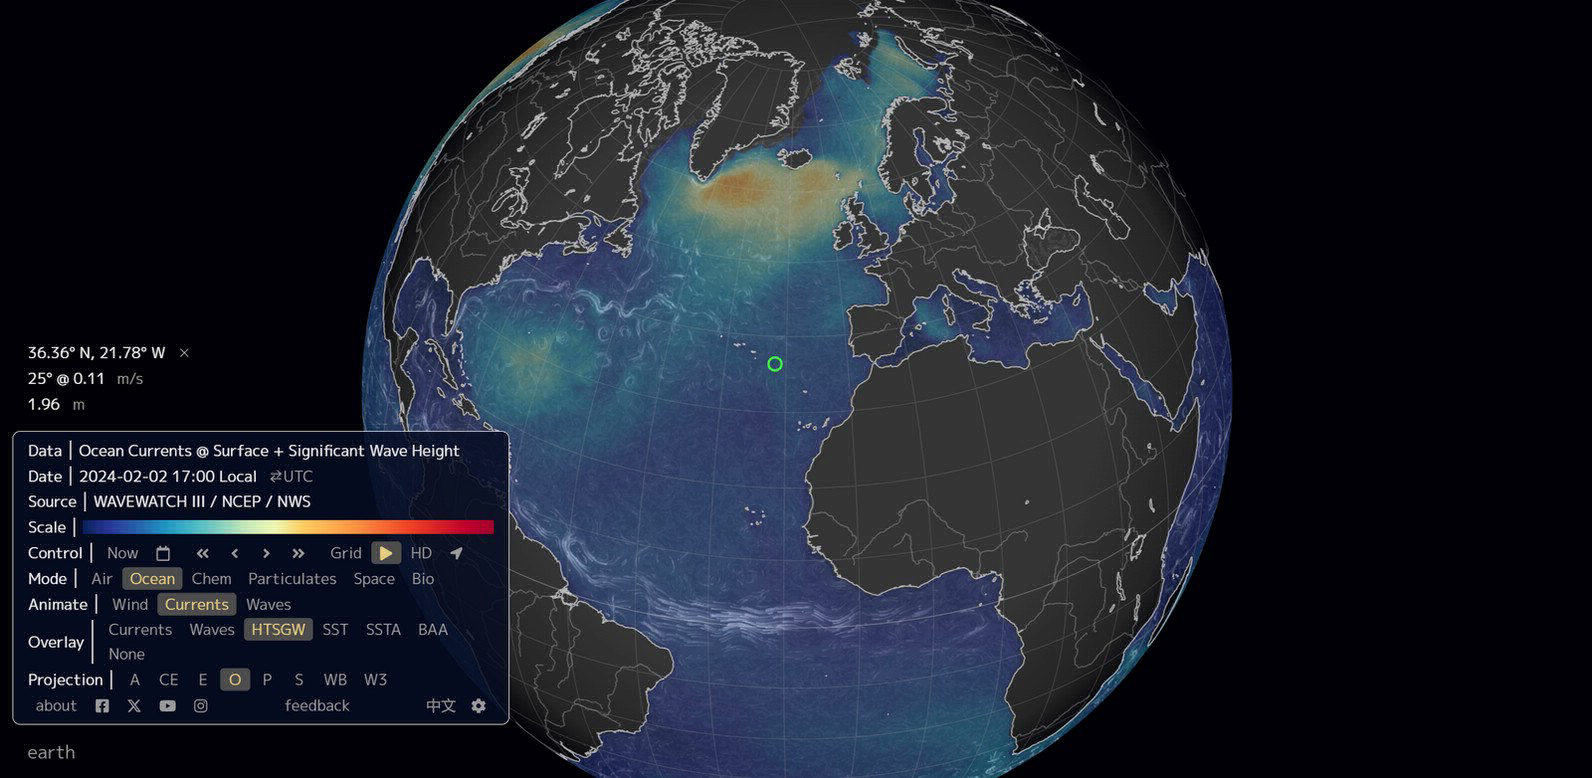
\includegraphics[width=382.4pt,height=186.85pt]{latexImage_85be5df54ea1df58d5f7ce83cc2ada8d.png}}
\put(227.6,-601.211){\fontsize{12}{1}\usefont{T1}{cmr}{m}{n}\selectfont\color{color_80434}图}
\put(242,-601.211){\fontsize{12}{1}\usefont{T1}{ptm}{m}{n}\selectfont\color{color_80434}3. }
\put(254,-601.211){\fontsize{12}{1}\usefont{T1}{cmr}{m}{n}\selectfont\color{color_80434}爱奥尼亚海洋流}
\put(56,-640.911){\fontsize{12}{1}\usefont{T1}{cmr}{m}{n}\selectfont\color{color_80434}}
\end{picture}
\begin{tikzpicture}[overlay]
\path(0pt,0pt);
\filldraw[color_283006][even odd rule]
(76.9pt, -643.661pt) -- (424.85pt, -643.661pt)
 -- (424.85pt, -643.661pt)
 -- (424.85pt, -629.711pt)
 -- (424.85pt, -629.711pt)
 -- (76.9pt, -629.711pt) -- cycle
;
\end{tikzpicture}
\begin{picture}(-5,0)(2.5,0)
\put(77,-640.911){\fontsize{12}{1}\usefont{T1}{cmr}{m}{n}\selectfont\color{color_54684}海底地}
\put(113,-640.911){\fontsize{12}{1}\usefont{T1}{cmr}{m}{n}\selectfont\color{color_54684}形}
\put(125,-640.911){\fontsize{12}{1}\usefont{T1}{cmr}{m}{n}\selectfont\color{color_54684}对潜水器}
\put(173,-640.911){\fontsize{12}{1}\usefont{T1}{cmr}{m}{n}\selectfont\color{color_54684}运}
\put(185,-640.911){\fontsize{12}{1}\usefont{T1}{cmr}{m}{n}\selectfont\color{color_54684}动的}
\put(209,-640.911){\fontsize{12}{1}\usefont{T1}{cmr}{m}{n}\selectfont\color{color_54684}影响}
\put(233,-640.911){\fontsize{12}{1}\usefont{T1}{cmr}{m}{n}\selectfont\color{color_54684}可以通过}
\put(281,-640.911){\fontsize{12}{1}\usefont{T1}{cmr}{m}{n}\selectfont\color{color_54684}调整浮}
\put(317,-640.911){\fontsize{12}{1}\usefont{T1}{cmr}{m}{n}\selectfont\color{color_54684}力和}
\put(341,-640.911){\fontsize{12}{1}\usefont{T1}{cmr}{m}{n}\selectfont\color{color_54684}阻}
\put(353,-640.911){\fontsize{12}{1}\usefont{T1}{cmr}{m}{n}\selectfont\color{color_54684}力参数}
\put(389,-640.911){\fontsize{12}{1}\usefont{T1}{cmr}{m}{n}\selectfont\color{color_54684}来}
\put(401,-640.911){\fontsize{12}{1}\usefont{T1}{cmr}{m}{n}\selectfont\color{color_54684}模拟}
\end{picture}
\newpage
\begin{tikzpicture}[overlay]\path(0pt,0pt);\end{tikzpicture}
\begin{picture}(-5,0)(2.5,0)
\put(78,-76.51099){\fontsize{16}{1}\usefont{T1}{ptm}{b}{n}\selectfont\color{color_55609}3}
\put(86,-76.51099){\fontsize{16}{1}\usefont{T1}{cmr}{m}{n}\selectfont\color{color_55609}、}
\put(119,-76.51099){\fontsize{16}{1}\usefont{T1}{cmr}{m}{n}\selectfont\color{color_55609}模型的建立}
\put(56,-106.511){\fontsize{14}{1}\usefont{T1}{cmr}{m}{n}\selectfont\color{color_55609}(}
\put(70,-106.511){\fontsize{14}{1}\usefont{T1}{ptm}{b}{n}\selectfont\color{color_55609}1}
\put(76.902,-106.511){\fontsize{14}{1}\usefont{T1}{ptm}{b}{n}\selectfont\color{color_55609})}
\put(81.592,-106.511){\fontsize{14}{1}\usefont{T1}{ptm}{b}{n}\selectfont\color{color_55609}.}
\put(85.1,-106.511){\fontsize{14}{1}\usefont{T1}{cmr}{m}{n}\selectfont\color{color_55609}坐}
\put(99.1,-106.511){\fontsize{14}{1}\usefont{T1}{cmr}{m}{n}\selectfont\color{color_55609}标系建立}
\put(56,-135.411){\fontsize{12}{1}\usefont{T1}{cmr}{m}{n}\selectfont\color{color_80434}在潜水器的建模过程中,}
\put(188,-135.411){\fontsize{12}{1}\usefont{T1}{cmr}{m}{n}\selectfont\color{color_80434}坐}
\put(200,-135.411){\fontsize{12}{1}\usefont{T1}{cmr}{m}{n}\selectfont\color{color_80434}标系的}
\put(236,-135.411){\fontsize{12}{1}\usefont{T1}{cmr}{m}{n}\selectfont\color{color_80434}选择}
\put(260,-135.411){\fontsize{12}{1}\usefont{T1}{cmr}{m}{n}\selectfont\color{color_80434}一}
\put(272,-135.411){\fontsize{12}{1}\usefont{T1}{cmr}{m}{n}\selectfont\color{color_80434}般包括两}
\put(320,-135.411){\fontsize{12}{1}\usefont{T1}{cmr}{m}{n}\selectfont\color{color_80434}个}
\put(332,-135.411){\fontsize{12}{1}\usefont{T1}{cmr}{m}{n}\selectfont\color{color_80434}坐}
\put(344,-135.411){\fontsize{12}{1}\usefont{T1}{cmr}{m}{n}\selectfont\color{color_80434}标系,即}
\put(392,-135.411){\fontsize{12}{1}\usefont{T1}{cmr}{m}{n}\selectfont\color{color_80434}固}
\put(404,-135.411){\fontsize{12}{1}\usefont{T1}{cmr}{m}{n}\selectfont\color{color_80434}定}
\put(416,-135.411){\fontsize{12}{1}\usefont{T1}{cmr}{m}{n}\selectfont\color{color_80434}坐}
\put(428,-135.411){\fontsize{12}{1}\usefont{T1}{cmr}{m}{n}\selectfont\color{color_80434}标系与}
\put(464,-135.411){\fontsize{12}{1}\usefont{T1}{cmr}{m}{n}\selectfont\color{color_80434}运}
\put(476,-135.411){\fontsize{12}{1}\usefont{T1}{cmr}{m}{n}\selectfont\color{color_80434}动}
\put(488,-135.411){\fontsize{12}{1}\usefont{T1}{cmr}{m}{n}\selectfont\color{color_80434}坐}
\put(56,-149.511){\fontsize{12}{1}\usefont{T1}{cmr}{m}{n}\selectfont\color{color_80434}标系,且}
\put(104,-149.511){\fontsize{12}{1}\usefont{T1}{cmr}{m}{n}\selectfont\color{color_80434}坐}
\put(116,-149.511){\fontsize{12}{1}\usefont{T1}{cmr}{m}{n}\selectfont\color{color_80434}标系的建立一}
\put(188,-149.511){\fontsize{12}{1}\usefont{T1}{cmr}{m}{n}\selectfont\color{color_80434}般符}
\put(212,-149.511){\fontsize{12}{1}\usefont{T1}{cmr}{m}{n}\selectfont\color{color_80434}合}
\put(224,-149.511){\fontsize{12}{1}\usefont{T1}{cmr}{m}{n}\selectfont\color{color_80434}右手}
\put(248,-149.511){\fontsize{12}{1}\usefont{T1}{cmr}{m}{n}\selectfont\color{color_80434}定}
\put(260,-149.511){\fontsize{12}{1}\usefont{T1}{cmr}{m}{n}\selectfont\color{color_80434}则}
\put(272,-149.511){\fontsize{12}{1}\usefont{T1}{ptm}{m}{n}\selectfont\color{color_80434}.}
\put(104.4,-389.661){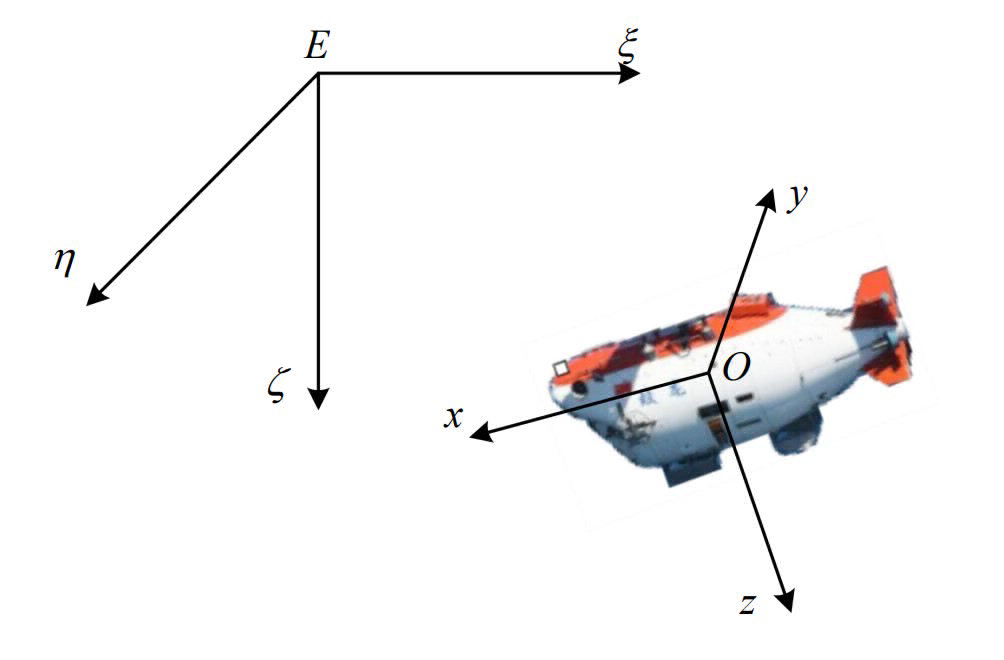
\includegraphics[width=356.55pt,height=234.4pt]{latexImage_ae6feac335c55f7ec916ff93667087d4.png}}
\put(232.1,-418.711){\fontsize{12}{1}\usefont{T1}{cmr}{m}{n}\selectfont\color{color_80434}图}
\put(246.5,-418.711){\fontsize{12}{1}\usefont{T1}{ptm}{m}{n}\selectfont\color{color_80434}4.  }
\put(261.5,-418.711){\fontsize{12}{1}\usefont{T1}{cmr}{m}{n}\selectfont\color{color_80434}潜水艇}
\put(297.5,-418.711){\fontsize{12}{1}\usefont{T1}{cmr}{m}{n}\selectfont\color{color_80434}坐}
\put(309.5,-418.711){\fontsize{12}{1}\usefont{T1}{cmr}{m}{n}\selectfont\color{color_80434}标系}
\put(56,-442.211){\fontsize{12}{1}\usefont{T1}{cmr}{m}{n}\selectfont\color{color_29791}在}
\put(68.084,-442.211){\fontsize{12}{1}\usefont{T1}{cmr}{m}{n}\selectfont\color{color_29791}对}
\put(80.276,-442.211){\fontsize{12}{1}\usefont{T1}{cmr}{m}{n}\selectfont\color{color_29791}潜}
\put(92.36,-442.211){\fontsize{12}{1}\usefont{T1}{cmr}{m}{n}\selectfont\color{color_29791}水}
\put(104.552,-442.211){\fontsize{12}{1}\usefont{T1}{cmr}{m}{n}\selectfont\color{color_29791}器}
\put(116.636,-442.211){\fontsize{12}{1}\usefont{T1}{cmr}{m}{n}\selectfont\color{color_29791}的}
\put(128.828,-442.211){\fontsize{12}{1}\usefont{T1}{cmr}{m}{n}\selectfont\color{color_29791}动}
\put(140.912,-442.211){\fontsize{12}{1}\usefont{T1}{cmr}{m}{n}\selectfont\color{color_29791}力}
\put(153.104,-442.211){\fontsize{12}{1}\usefont{T1}{cmr}{m}{n}\selectfont\color{color_29791}学}
\put(165.188,-442.211){\fontsize{12}{1}\usefont{T1}{cmr}{m}{n}\selectfont\color{color_29791}问}
\put(177.38,-442.211){\fontsize{12}{1}\usefont{T1}{cmr}{m}{n}\selectfont\color{color_29791}题}
\put(189.464,-442.211){\fontsize{12}{1}\usefont{T1}{cmr}{m}{n}\selectfont\color{color_29791}进}
\put(201.656,-442.211){\fontsize{12}{1}\usefont{T1}{cmr}{m}{n}\selectfont\color{color_29791}行}
\put(213.9,-442.211){\fontsize{12}{1}\usefont{T1}{cmr}{m}{n}\selectfont\color{color_29791}研}
\put(226.092,-442.211){\fontsize{12}{1}\usefont{T1}{cmr}{m}{n}\selectfont\color{color_29791}究}
\put(238.2,-442.211){\fontsize{12}{1}\usefont{T1}{cmr}{m}{n}\selectfont\color{color_29791}时}
\put(250.392,-442.211){\fontsize{12}{1}\usefont{T1}{cmr}{m}{n}\selectfont\color{color_29791},}
\put(262.476,-442.211){\fontsize{12}{1}\usefont{T1}{cmr}{m}{n}\selectfont\color{color_29791}通}
\put(274.668,-442.211){\fontsize{12}{1}\usefont{T1}{cmr}{m}{n}\selectfont\color{color_29791}常}
\put(286.8,-442.211){\fontsize{12}{1}\usefont{T1}{cmr}{m}{n}\selectfont\color{color_29791}选}
\put(298.992,-442.211){\fontsize{12}{1}\usefont{T1}{cmr}{m}{n}\selectfont\color{color_29791}择}
\put(311.076,-442.211){\fontsize{12}{1}\usefont{T1}{cmr}{m}{n}\selectfont\color{color_29791}大}
\put(323.3,-442.211){\fontsize{12}{1}\usefont{T1}{cmr}{m}{n}\selectfont\color{color_29791}地}
\put(335.4,-442.211){\fontsize{12}{1}\usefont{T1}{cmr}{m}{n}\selectfont\color{color_29791}作}
\put(347.6,-442.211){\fontsize{12}{1}\usefont{T1}{cmr}{m}{n}\selectfont\color{color_29791}为}
\put(359.684,-442.211){\fontsize{12}{1}\usefont{T1}{cmr}{m}{n}\selectfont\color{color_29791}参}
\put(371.9,-442.211){\fontsize{12}{1}\usefont{T1}{cmr}{m}{n}\selectfont\color{color_29791}考}
\put(384,-442.211){\fontsize{12}{1}\usefont{T1}{cmr}{m}{n}\selectfont\color{color_29791}系}
\put(397,-442.211){\fontsize{12}{1}\usefont{T1}{ptm}{m}{n}\selectfont\color{color_29791}.}
\put(400.1,-442.211){\fontsize{12}{1}\usefont{T1}{cmr}{m}{n}\selectfont\color{color_29791}载}
\put(412.292,-442.211){\fontsize{12}{1}\usefont{T1}{cmr}{m}{n}\selectfont\color{color_29791}人}
\put(424.4,-442.211){\fontsize{12}{1}\usefont{T1}{cmr}{m}{n}\selectfont\color{color_29791}潜}
\put(436.592,-442.211){\fontsize{12}{1}\usefont{T1}{cmr}{m}{n}\selectfont\color{color_29791}水}
\put(448.676,-442.211){\fontsize{12}{1}\usefont{T1}{cmr}{m}{n}\selectfont\color{color_29791}器}
\put(460.868,-442.211){\fontsize{12}{1}\usefont{T1}{cmr}{m}{n}\selectfont\color{color_29791}的}
\put(473,-442.211){\fontsize{12}{1}\usefont{T1}{cmr}{m}{n}\selectfont\color{color_29791}固}
\put(485.2,-442.211){\fontsize{12}{1}\usefont{T1}{cmr}{m}{n}\selectfont\color{color_29791}定}
\put(497.3,-442.211){\fontsize{12}{1}\usefont{T1}{cmr}{m}{n}\selectfont\color{color_29791}坐}
\put(56,-463.511){\fontsize{12}{1}\usefont{T1}{cmr}{m}{n}\selectfont\color{color_29791}标}
\put(68.192,-463.511){\fontsize{12}{1}\usefont{T1}{cmr}{m}{n}\selectfont\color{color_29791}系}
\put(80.48,-463.511){\fontsize{12}{1}\usefont{T1}{cmr}{m}{n}\selectfont\color{color_29791}与}
\put(92.672,-463.511){\fontsize{12}{1}\usefont{T1}{cmr}{m}{n}\selectfont\color{color_29791}机}
\put(105,-463.511){\fontsize{12}{1}\usefont{T1}{cmr}{m}{n}\selectfont\color{color_29791}体}
\put(117.192,-463.511){\fontsize{12}{1}\usefont{T1}{cmr}{m}{n}\selectfont\color{color_29791}坐}
\put(129.5,-463.511){\fontsize{12}{1}\usefont{T1}{cmr}{m}{n}\selectfont\color{color_29791}标}
\put(141.692,-463.511){\fontsize{12}{1}\usefont{T1}{cmr}{m}{n}\selectfont\color{color_29791}系}
\put(153.98,-463.511){\fontsize{12}{1}\usefont{T1}{cmr}{m}{n}\selectfont\color{color_29791}的}
\put(166.2,-463.511){\fontsize{12}{1}\usefont{T1}{cmr}{m}{n}\selectfont\color{color_29791}选}
\put(178.488,-463.511){\fontsize{12}{1}\usefont{T1}{cmr}{m}{n}\selectfont\color{color_29791}取}
\put(190.7,-463.511){\fontsize{12}{1}\usefont{T1}{cmr}{m}{n}\selectfont\color{color_29791}如}
\put(203,-463.511){\fontsize{12}{1}\usefont{T1}{cmr}{m}{n}\selectfont\color{color_29791}图}
\put(217.9,-463.511){\fontsize{12}{1}\usefont{T1}{ptm}{m}{n}\selectfont\color{color_29791}1}
\put(226.5,-463.511){\fontsize{12}{1}\usefont{T1}{cmr}{m}{n}\selectfont\color{color_29791}所}
\put(238.788,-463.511){\fontsize{12}{1}\usefont{T1}{cmr}{m}{n}\selectfont\color{color_29791}示}
\put(251,-463.511){\fontsize{12}{1}\usefont{T1}{cmr}{m}{n}\selectfont\color{color_29791}。}
\put(263.3,-463.511){\fontsize{12}{1}\usefont{T1}{cmr}{m}{n}\selectfont\color{color_29791}固}
\put(275.5,-463.511){\fontsize{12}{1}\usefont{T1}{cmr}{m}{n}\selectfont\color{color_29791}定}
\put(287.8,-463.511){\fontsize{12}{1}\usefont{T1}{cmr}{m}{n}\selectfont\color{color_29791}坐}
\put(300,-463.511){\fontsize{12}{1}\usefont{T1}{cmr}{m}{n}\selectfont\color{color_29791}标}
\put(312.288,-463.511){\fontsize{12}{1}\usefont{T1}{cmr}{m}{n}\selectfont\color{color_29791}系}
\put(387,-463.511){\fontsize{12}{1}\usefont{T1}{cmr}{m}{n}\selectfont\color{color_29791}的}
\put(399.2,-463.511){\fontsize{12}{1}\usefont{T1}{cmr}{m}{n}\selectfont\color{color_29791}原}
\put(411.5,-463.511){\fontsize{12}{1}\usefont{T1}{cmr}{m}{n}\selectfont\color{color_29791}点}
\put(426.2,-463.511){\fontsize{12}{1}\usefont{T1}{ptm}{m}{n}\selectfont\color{color_29791}E}
\put(436.2,-463.511){\fontsize{12}{1}\usefont{T1}{cmr}{m}{n}\selectfont\color{color_29791}根}
\put(448.392,-463.511){\fontsize{12}{1}\usefont{T1}{cmr}{m}{n}\selectfont\color{color_29791}据}
\put(460.7,-463.511){\fontsize{12}{1}\usefont{T1}{cmr}{m}{n}\selectfont\color{color_29791}实}
\put(472.892,-463.511){\fontsize{12}{1}\usefont{T1}{cmr}{m}{n}\selectfont\color{color_29791}际}
\put(485.2,-463.511){\fontsize{12}{1}\usefont{T1}{cmr}{m}{n}\selectfont\color{color_29791}情}
\put(497.392,-463.511){\fontsize{12}{1}\usefont{T1}{cmr}{m}{n}\selectfont\color{color_29791}况}
\put(140,-484.011){\fontsize{12}{1}\usefont{T1}{cmr}{m}{n}\selectfont\color{color_29791} }
\put(56,-484.011){\fontsize{12}{1}\usefont{T1}{cmr}{m}{n}\selectfont\color{color_29791}取}
\put(68,-484.011){\fontsize{12}{1}\usefont{T1}{cmr}{m}{n}\selectfont\color{color_29791}海面上一点,}
\put(165.7,-484.011){\fontsize{12}{1}\usefont{T1}{cmr}{m}{n}\selectfont\color{color_29791}轴正}
\put(189.7,-484.011){\fontsize{12}{1}\usefont{T1}{cmr}{m}{n}\selectfont\color{color_29791}向指向地}
\put(237.7,-484.011){\fontsize{12}{1}\usefont{T1}{cmr}{m}{n}\selectfont\color{color_29791}心}
\put(249.7,-484.011){\fontsize{12}{1}\usefont{T1}{cmr}{m}{n}\selectfont\color{color_29791},}
\put(283.6,-484.011){\fontsize{12}{1}\usefont{T1}{cmr}{m}{n}\selectfont\color{color_29791}轴}
\put(295.6,-484.011){\fontsize{12}{1}\usefont{T1}{cmr}{m}{n}\selectfont\color{color_29791}指向地理}
\put(343.6,-484.011){\fontsize{12}{1}\usefont{T1}{cmr}{m}{n}\selectfont\color{color_29791}北}
\put(355.6,-484.011){\fontsize{12}{1}\usefont{T1}{cmr}{m}{n}\selectfont\color{color_29791},}
\put(389.4,-484.011){\fontsize{12}{1}\usefont{T1}{cmr}{m}{n}\selectfont\color{color_29791}轴}
\put(401.4,-484.011){\fontsize{12}{1}\usefont{T1}{cmr}{m}{n}\selectfont\color{color_29791}指向}
\put(425.4,-484.011){\fontsize{12}{1}\usefont{T1}{cmr}{m}{n}\selectfont\color{color_29791}东}
\put(437.4,-484.011){\fontsize{12}{1}\usefont{T1}{cmr}{m}{n}\selectfont\color{color_29791},}
\put(449.4,-484.011){\fontsize{12}{1}\usefont{T1}{cmr}{m}{n}\selectfont\color{color_29791}构}
\put(461.4,-484.011){\fontsize{12}{1}\usefont{T1}{cmr}{m}{n}\selectfont\color{color_29791}成}
\put(473.4,-484.011){\fontsize{12}{1}\usefont{T1}{cmr}{m}{n}\selectfont\color{color_29791}右手直}
\put(56,-503.711){\fontsize{12}{1}\usefont{T1}{cmr}{m}{n}\selectfont\color{color_29791}角坐}
\put(80,-503.711){\fontsize{12}{1}\usefont{T1}{cmr}{m}{n}\selectfont\color{color_29791}标系}
\put(104,-503.711){\fontsize{12}{1}\usefont{T1}{ptm}{m}{n}\selectfont\color{color_29791}.}
\put(56,-527.711){\fontsize{12}{1}\usefont{T1}{cmr}{m}{n}\selectfont\color{color_29791}机}
\put(68.1,-527.711){\fontsize{12}{1}\usefont{T1}{cmr}{m}{n}\selectfont\color{color_29791}体}
\put(80.184,-527.711){\fontsize{12}{1}\usefont{T1}{cmr}{m}{n}\selectfont\color{color_29791}坐}
\put(92.3,-527.711){\fontsize{12}{1}\usefont{T1}{cmr}{m}{n}\selectfont\color{color_29791}标}
\put(104.384,-527.711){\fontsize{12}{1}\usefont{T1}{cmr}{m}{n}\selectfont\color{color_29791}系}
\put(158,-527.711){\fontsize{12}{1}\usefont{T1}{cmr}{m}{n}\selectfont\color{color_29791} }
\put(161.9,-527.711){\fontsize{12}{1}\usefont{T1}{cmr}{m}{n}\selectfont\color{color_29791}的}
\put(174,-527.711){\fontsize{12}{1}\usefont{T1}{cmr}{m}{n}\selectfont\color{color_29791}原}
\put(186.1,-527.711){\fontsize{12}{1}\usefont{T1}{cmr}{m}{n}\selectfont\color{color_29791}点}
\put(208.1,-527.711){\fontsize{12}{1}\usefont{T1}{cmr}{m}{n}\selectfont\color{color_29791}取}
\put(220.2,-527.711){\fontsize{12}{1}\usefont{T1}{cmr}{m}{n}\selectfont\color{color_29791}潜}
\put(232.284,-527.711){\fontsize{12}{1}\usefont{T1}{cmr}{m}{n}\selectfont\color{color_29791}水}
\put(244.368,-527.711){\fontsize{12}{1}\usefont{T1}{cmr}{m}{n}\selectfont\color{color_29791}器}
\put(256.452,-527.711){\fontsize{12}{1}\usefont{T1}{cmr}{m}{n}\selectfont\color{color_29791}主}
\put(268.5359,-527.711){\fontsize{12}{1}\usefont{T1}{cmr}{m}{n}\selectfont\color{color_29791}对}
\put(280.7,-527.711){\fontsize{12}{1}\usefont{T1}{cmr}{m}{n}\selectfont\color{color_29791}称}
\put(292.8,-527.711){\fontsize{12}{1}\usefont{T1}{cmr}{m}{n}\selectfont\color{color_29791}轴}
\put(304.9,-527.711){\fontsize{12}{1}\usefont{T1}{cmr}{m}{n}\selectfont\color{color_29791}的}
\put(316.984,-527.711){\fontsize{12}{1}\usefont{T1}{cmr}{m}{n}\selectfont\color{color_29791}中}
\put(329.068,-527.711){\fontsize{12}{1}\usefont{T1}{cmr}{m}{n}\selectfont\color{color_29791}点}
\put(341.152,-527.711){\fontsize{12}{1}\usefont{T1}{cmr}{m}{n}\selectfont\color{color_29791},}
\put(371.9,-527.711){\fontsize{12}{1}\usefont{T1}{cmr}{m}{n}\selectfont\color{color_29791} }
\put(375.8,-527.711){\fontsize{12}{1}\usefont{T1}{cmr}{m}{n}\selectfont\color{color_29791}轴}
\put(387.9,-527.711){\fontsize{12}{1}\usefont{T1}{cmr}{m}{n}\selectfont\color{color_29791}与}
\put(399.984,-527.711){\fontsize{12}{1}\usefont{T1}{cmr}{m}{n}\selectfont\color{color_29791}潜}
\put(412.068,-527.711){\fontsize{12}{1}\usefont{T1}{cmr}{m}{n}\selectfont\color{color_29791}水}
\put(424.152,-527.711){\fontsize{12}{1}\usefont{T1}{cmr}{m}{n}\selectfont\color{color_29791}器}
\put(436.236,-527.711){\fontsize{12}{1}\usefont{T1}{cmr}{m}{n}\selectfont\color{color_29791}主}
\put(448.3199,-527.711){\fontsize{12}{1}\usefont{T1}{cmr}{m}{n}\selectfont\color{color_29791}对}
\put(460.5,-527.711){\fontsize{12}{1}\usefont{T1}{cmr}{m}{n}\selectfont\color{color_29791}称}
\put(472.6,-527.711){\fontsize{12}{1}\usefont{T1}{cmr}{m}{n}\selectfont\color{color_29791}轴}
\put(484.7,-527.711){\fontsize{12}{1}\usefont{T1}{cmr}{m}{n}\selectfont\color{color_29791}重}
\put(496.784,-527.711){\fontsize{12}{1}\usefont{T1}{cmr}{m}{n}\selectfont\color{color_29791}合}
\put(509.5,-527.711){\fontsize{12}{1}\usefont{T1}{cmr}{m}{n}\selectfont\color{color_29791},}
\put(56,-548.211){\fontsize{12}{1}\usefont{T1}{cmr}{m}{n}\selectfont\color{color_29791}指}
\put(68.084,-548.211){\fontsize{12}{1}\usefont{T1}{cmr}{m}{n}\selectfont\color{color_29791}向}
\put(80.168,-548.211){\fontsize{12}{1}\usefont{T1}{cmr}{m}{n}\selectfont\color{color_29791}潜}
\put(92.252,-548.211){\fontsize{12}{1}\usefont{T1}{cmr}{m}{n}\selectfont\color{color_29791}水}
\put(104.336,-548.211){\fontsize{12}{1}\usefont{T1}{cmr}{m}{n}\selectfont\color{color_29791}器}
\put(116.5,-548.211){\fontsize{12}{1}\usefont{T1}{cmr}{m}{n}\selectfont\color{color_29791}艏}
\put(128.6,-548.211){\fontsize{12}{1}\usefont{T1}{cmr}{m}{n}\selectfont\color{color_29791}部}
\put(140.684,-548.211){\fontsize{12}{1}\usefont{T1}{cmr}{m}{n}\selectfont\color{color_29791},}
\put(169.6,-548.211){\fontsize{12}{1}\usefont{T1}{cmr}{m}{n}\selectfont\color{color_29791} }
\put(173.5,-548.211){\fontsize{12}{1}\usefont{T1}{cmr}{m}{n}\selectfont\color{color_29791}轴}
\put(185.6,-548.211){\fontsize{12}{1}\usefont{T1}{cmr}{m}{n}\selectfont\color{color_29791}与}
\put(197.7,-548.211){\fontsize{12}{1}\usefont{T1}{cmr}{m}{n}\selectfont\color{color_29791}辅}
\put(209.784,-548.211){\fontsize{12}{1}\usefont{T1}{cmr}{m}{n}\selectfont\color{color_29791}助}
\put(221.9,-548.211){\fontsize{12}{1}\usefont{T1}{cmr}{m}{n}\selectfont\color{color_29791}对}
\put(234,-548.211){\fontsize{12}{1}\usefont{T1}{cmr}{m}{n}\selectfont\color{color_29791}称}
\put(246.1,-548.211){\fontsize{12}{1}\usefont{T1}{cmr}{m}{n}\selectfont\color{color_29791}轴}
\put(258.2,-548.211){\fontsize{12}{1}\usefont{T1}{cmr}{m}{n}\selectfont\color{color_29791}重}
\put(270.284,-548.211){\fontsize{12}{1}\usefont{T1}{cmr}{m}{n}\selectfont\color{color_29791}合}
\put(282.368,-548.211){\fontsize{12}{1}\usefont{T1}{cmr}{m}{n}\selectfont\color{color_29791}并}
\put(294.452,-548.211){\fontsize{12}{1}\usefont{T1}{cmr}{m}{n}\selectfont\color{color_29791}指}
\put(306.5359,-548.211){\fontsize{12}{1}\usefont{T1}{cmr}{m}{n}\selectfont\color{color_29791}向}
\put(318.6199,-548.211){\fontsize{12}{1}\usefont{T1}{cmr}{m}{n}\selectfont\color{color_29791}潜}
\put(330.7039,-548.211){\fontsize{12}{1}\usefont{T1}{cmr}{m}{n}\selectfont\color{color_29791}水}
\put(342.7879,-548.211){\fontsize{12}{1}\usefont{T1}{cmr}{m}{n}\selectfont\color{color_29791}器}
\put(355,-548.211){\fontsize{12}{1}\usefont{T1}{cmr}{m}{n}\selectfont\color{color_29791}前}
\put(367.1,-548.211){\fontsize{12}{1}\usefont{T1}{cmr}{m}{n}\selectfont\color{color_29791}进}
\put(379.184,-548.211){\fontsize{12}{1}\usefont{T1}{cmr}{m}{n}\selectfont\color{color_29791}方}
\put(391.268,-548.211){\fontsize{12}{1}\usefont{T1}{cmr}{m}{n}\selectfont\color{color_29791}向}
\put(403.4,-548.211){\fontsize{12}{1}\usefont{T1}{cmr}{m}{n}\selectfont\color{color_29791}右}
\put(415.5,-548.211){\fontsize{12}{1}\usefont{T1}{cmr}{m}{n}\selectfont\color{color_29791}侧}
\put(427.584,-548.211){\fontsize{12}{1}\usefont{T1}{cmr}{m}{n}\selectfont\color{color_29791},}
\put(457.2,-548.211){\fontsize{12}{1}\usefont{T1}{cmr}{m}{n}\selectfont\color{color_29791} }
\put(461.1,-548.211){\fontsize{12}{1}\usefont{T1}{cmr}{m}{n}\selectfont\color{color_29791}轴}
\put(473.2,-548.211){\fontsize{12}{1}\usefont{T1}{cmr}{m}{n}\selectfont\color{color_29791}垂}
\put(485.3,-548.211){\fontsize{12}{1}\usefont{T1}{cmr}{m}{n}\selectfont\color{color_29791}直}
\put(497.4,-548.211){\fontsize{12}{1}\usefont{T1}{cmr}{m}{n}\selectfont\color{color_29791}于}
\put(56,-568.711){\fontsize{12}{1}\usefont{T1}{cmr}{m}{n}\selectfont\color{color_29791}水}
\put(68,-568.711){\fontsize{12}{1}\usefont{T1}{cmr}{m}{n}\selectfont\color{color_29791}线}
\put(80,-568.711){\fontsize{12}{1}\usefont{T1}{cmr}{m}{n}\selectfont\color{color_29791}面,指向潜水器底部方向,}
\put(271.3,-568.711){\fontsize{12}{1}\usefont{T1}{cmr}{m}{n}\selectfont\color{color_29791}同}
\put(283.3,-568.711){\fontsize{12}{1}\usefont{T1}{cmr}{m}{n}\selectfont\color{color_29791}样}
\put(295.3,-568.711){\fontsize{12}{1}\usefont{T1}{cmr}{m}{n}\selectfont\color{color_29791}构}
\put(307.3,-568.711){\fontsize{12}{1}\usefont{T1}{cmr}{m}{n}\selectfont\color{color_29791}成}
\put(319.3,-568.711){\fontsize{12}{1}\usefont{T1}{cmr}{m}{n}\selectfont\color{color_29791}右手直角坐}
\put(379.3,-568.711){\fontsize{12}{1}\usefont{T1}{cmr}{m}{n}\selectfont\color{color_29791}标系}
\put(403.3,-568.711){\fontsize{12}{1}\usefont{T1}{ptm}{m}{n}\selectfont\color{color_29791}.}
\put(56,-606.111){\fontsize{14}{1}\usefont{T1}{cmr}{m}{n}\selectfont\color{color_55609}(}
\put(70,-606.111){\fontsize{14}{1}\usefont{T1}{ptm}{b}{n}\selectfont\color{color_55609}2}
\put(76.902,-606.111){\fontsize{14}{1}\usefont{T1}{ptm}{b}{n}\selectfont\color{color_55609})}
\put(81.592,-606.111){\fontsize{14}{1}\usefont{T1}{ptm}{b}{n}\selectfont\color{color_55609}.}
\put(85.1,-606.111){\fontsize{14}{1}\usefont{T1}{cmr}{m}{n}\selectfont\color{color_55609}动力学方程}
\put(56,-638.211){\fontsize{12}{1}\usefont{T1}{cmr}{m}{n}\selectfont\color{color_80434}考虑}
\put(80,-638.211){\fontsize{12}{1}\usefont{T1}{cmr}{m}{n}\selectfont\color{color_80434}潜水艇的动力学,可以使用}
\put(224,-638.211){\fontsize{12}{1}\usefont{T1}{cmr}{m}{n}\selectfont\color{color_80434}牛顿第}
\put(260,-638.211){\fontsize{12}{1}\usefont{T1}{cmr}{m}{n}\selectfont\color{color_80434}二定}
\put(284,-638.211){\fontsize{12}{1}\usefont{T1}{cmr}{m}{n}\selectfont\color{color_80434}律}
\put(296,-638.211){\fontsize{12}{1}\usefont{T1}{cmr}{m}{n}\selectfont\color{color_80434}表}
\put(308,-638.211){\fontsize{12}{1}\usefont{T1}{cmr}{m}{n}\selectfont\color{color_80434}示}
\put(320,-638.211){\fontsize{12}{1}\usefont{T1}{cmr}{m}{n}\selectfont\color{color_80434}潜艇的动力学方程:}
\put(56,-705.711){\fontsize{12}{1}\usefont{T1}{cmr}{m}{n}\selectfont\color{color_80434}其}
\put(68,-705.711){\fontsize{12}{1}\usefont{T1}{cmr}{m}{n}\selectfont\color{color_80434}中,}
\put(99.5,-705.711){\fontsize{12}{1}\usefont{T1}{cmr}{m}{n}\selectfont\color{color_80434}是}
\put(111.5,-705.711){\fontsize{12}{1}\usefont{T1}{cmr}{m}{n}\selectfont\color{color_80434}潜水器的位置向}
\put(195.5,-705.711){\fontsize{12}{1}\usefont{T1}{cmr}{m}{n}\selectfont\color{color_80434}量}
\put(207.5,-705.711){\fontsize{12}{1}\usefont{T1}{cmr}{m}{n}\selectfont\color{color_80434},}
\put(224.1,-705.711){\fontsize{12}{1}\usefont{T1}{cmr}{m}{n}\selectfont\color{color_80434}是}
\put(236.1,-705.711){\fontsize{12}{1}\usefont{T1}{cmr}{m}{n}\selectfont\color{color_80434}潜水器}
\put(272.1,-705.711){\fontsize{12}{1}\usefont{T1}{cmr}{m}{n}\selectfont\color{color_80434}运}
\put(284.1,-705.711){\fontsize{12}{1}\usefont{T1}{cmr}{m}{n}\selectfont\color{color_80434}动的时间}
\put(332.1,-705.711){\fontsize{12}{1}\usefont{T1}{ptm}{m}{n}\selectfont\color{color_80434};}
\put(67.3,-729.211){\fontsize{12}{1}\usefont{T1}{cmr}{m}{n}\selectfont\color{color_80434}是}
\put(79.3,-729.211){\fontsize{12}{1}\usefont{T1}{cmr}{m}{n}\selectfont\color{color_80434}潜水艇的}
\put(127.3,-729.211){\fontsize{12}{1}\usefont{T1}{cmr}{m}{n}\selectfont\color{color_80434}质量}
\put(151.3,-729.211){\fontsize{12}{1}\usefont{T1}{ptm}{m}{n}\selectfont\color{color_80434};}
\end{picture}
\newpage
\begin{tikzpicture}[overlay]
\path(0pt,0pt);
\filldraw[color_283006][even odd rule]
(106.2pt, -79.56097pt) -- (190.15pt, -79.56097pt)
 -- (190.15pt, -79.56097pt)
 -- (190.15pt, -65.61096pt)
 -- (190.15pt, -65.61096pt)
 -- (106.2pt, -65.61096pt) -- cycle
;
\end{tikzpicture}
\begin{picture}(-5,0)(2.5,0)
\put(106.3,-76.81097){\fontsize{12}{1}\usefont{T1}{cmr}{m}{n}\selectfont\color{color_54684}是}
\put(118.3,-76.81097){\fontsize{12}{1}\usefont{T1}{cmr}{m}{n}\selectfont\color{color_54684}潜水艇的重力}
\end{picture}
\begin{tikzpicture}[overlay]
\path(0pt,0pt);
\filldraw[color_283006][even odd rule]
(190.2pt, -79.56097pt) -- (194.15pt, -79.56097pt)
 -- (194.15pt, -79.56097pt)
 -- (194.15pt, -65.61096pt)
 -- (194.15pt, -65.61096pt)
 -- (190.2pt, -65.61096pt) -- cycle
;
\end{tikzpicture}
\begin{picture}(-5,0)(2.5,0)
\put(190.3,-76.81097){\fontsize{12}{1}\usefont{T1}{cmr}{m}{n}\selectfont\color{color_54684};}
\put(69.5,-99.51099){\fontsize{12}{1}\usefont{T1}{cmr}{m}{n}\selectfont\color{color_80434}是}
\end{picture}
\begin{tikzpicture}[overlay]
\path(0pt,0pt);
\filldraw[color_283006][even odd rule]
(81.4pt, -102.361pt) -- (201.35pt, -102.361pt)
 -- (201.35pt, -102.361pt)
 -- (201.35pt, -88.41101pt)
 -- (201.35pt, -88.41101pt)
 -- (81.4pt, -88.41101pt) -- cycle
;
\end{tikzpicture}
\begin{picture}(-5,0)(2.5,0)
\put(81.5,-99.51099){\fontsize{12}{1}\usefont{T1}{cmr}{m}{n}\selectfont\color{color_54684}水流对潜水器的}
\put(165.5,-99.51099){\fontsize{12}{1}\usefont{T1}{cmr}{m}{n}\selectfont\color{color_54684}作}
\put(177.5,-99.51099){\fontsize{12}{1}\usefont{T1}{cmr}{m}{n}\selectfont\color{color_54684}用力}
\end{picture}
\begin{tikzpicture}[overlay]
\path(0pt,0pt);
\filldraw[color_283006][even odd rule]
(201.4pt, -102.361pt) -- (205.35pt, -102.361pt)
 -- (205.35pt, -102.361pt)
 -- (205.35pt, -88.41101pt)
 -- (205.35pt, -88.41101pt)
 -- (201.4pt, -88.41101pt) -- cycle
;
\end{tikzpicture}
\begin{picture}(-5,0)(2.5,0)
\put(201.5,-99.51099){\fontsize{12}{1}\usefont{T1}{cmr}{m}{n}\selectfont\color{color_54684};}
\end{picture}
\begin{tikzpicture}[overlay]
\path(0pt,0pt);
\filldraw[color_283006][even odd rule]
(55.9pt, -125.861pt) -- (79.85001pt, -125.861pt)
 -- (79.85001pt, -125.861pt)
 -- (79.85001pt, -111.911pt)
 -- (79.85001pt, -111.911pt)
 -- (55.9pt, -111.911pt) -- cycle
;
\end{tikzpicture}
\begin{picture}(-5,0)(2.5,0)
\put(56,-123.011){\fontsize{12}{1}\usefont{T1}{cmr}{m}{n}\selectfont\color{color_54684}浮}
\put(68,-123.011){\fontsize{12}{1}\usefont{T1}{cmr}{m}{n}\selectfont\color{color_54684}力}
\end{picture}
\begin{tikzpicture}[overlay]
\path(0pt,0pt);
\filldraw[color_283006][even odd rule]
(79.9pt, -125.861pt) -- (83.65pt, -125.861pt)
 -- (83.65pt, -125.861pt)
 -- (83.65pt, -111.911pt)
 -- (83.65pt, -111.911pt)
 -- (79.9pt, -111.911pt) -- cycle
;
\end{tikzpicture}
\begin{picture}(-5,0)(2.5,0)
\put(80,-123.011){\fontsize{12}{1}\usefont{T1}{cmr}{m}{n}\selectfont\color{color_54684} }
\end{picture}
\begin{tikzpicture}[overlay]
\path(0pt,0pt);
\filldraw[color_283006][even odd rule]
(97.2pt, -125.861pt) -- (313.15pt, -125.861pt)
 -- (313.15pt, -125.861pt)
 -- (313.15pt, -111.911pt)
 -- (313.15pt, -111.911pt)
 -- (97.2pt, -111.911pt) -- cycle
;
\end{tikzpicture}
\begin{picture}(-5,0)(2.5,0)
\put(97.3,-123.011){\fontsize{12}{1}\usefont{T1}{cmr}{m}{n}\selectfont\color{color_54684}可以通过潜水器}
\put(181.3,-123.011){\fontsize{12}{1}\usefont{T1}{cmr}{m}{n}\selectfont\color{color_54684}排}
\put(193.3,-123.011){\fontsize{12}{1}\usefont{T1}{cmr}{m}{n}\selectfont\color{color_54684}水}
\put(205.3,-123.011){\fontsize{12}{1}\usefont{T1}{cmr}{m}{n}\selectfont\color{color_54684}量}
\put(217.3,-123.011){\fontsize{12}{1}\usefont{T1}{cmr}{m}{n}\selectfont\color{color_54684}和水的}
\put(253.3,-123.011){\fontsize{12}{1}\usefont{T1}{cmr}{m}{n}\selectfont\color{color_54684}密度来}
\put(289.3,-123.011){\fontsize{12}{1}\usefont{T1}{cmr}{m}{n}\selectfont\color{color_54684}计算}
\end{picture}
\begin{tikzpicture}[overlay]
\path(0pt,0pt);
\filldraw[color_283006][even odd rule]
(313.2pt, -125.861pt) -- (317.15pt, -125.861pt)
 -- (317.15pt, -125.861pt)
 -- (317.15pt, -111.911pt)
 -- (317.15pt, -111.911pt)
 -- (313.2pt, -111.911pt) -- cycle
;
\end{tikzpicture}
\begin{picture}(-5,0)(2.5,0)
\put(313.3,-123.011){\fontsize{12}{1}\usefont{T1}{cmr}{m}{n}\selectfont\color{color_54684};}
\end{picture}
\begin{tikzpicture}[overlay]
\path(0pt,0pt);
\filldraw[color_283006][even odd rule]
(55.9pt, -149.361pt) -- (79.85001pt, -149.361pt)
 -- (79.85001pt, -149.361pt)
 -- (79.85001pt, -135.411pt)
 -- (79.85001pt, -135.411pt)
 -- (55.9pt, -135.411pt) -- cycle
;
\end{tikzpicture}
\begin{picture}(-5,0)(2.5,0)
\put(56,-146.511){\fontsize{12}{1}\usefont{T1}{cmr}{m}{n}\selectfont\color{color_54684}阻}
\put(68,-146.511){\fontsize{12}{1}\usefont{T1}{cmr}{m}{n}\selectfont\color{color_54684}力}
\end{picture}
\begin{tikzpicture}[overlay]
\path(0pt,0pt);
\filldraw[color_283006][even odd rule]
(79.9pt, -149.361pt) -- (83.65pt, -149.361pt)
 -- (83.65pt, -149.361pt)
 -- (83.65pt, -135.411pt)
 -- (83.65pt, -135.411pt)
 -- (79.9pt, -135.411pt) -- cycle
;
\end{tikzpicture}
\begin{picture}(-5,0)(2.5,0)
\put(80,-146.511){\fontsize{12}{1}\usefont{T1}{cmr}{m}{n}\selectfont\color{color_54684} }
\end{picture}
\begin{tikzpicture}[overlay]
\path(0pt,0pt);
\filldraw[color_283006][even odd rule]
(98pt, -149.361pt) -- (100.15pt, -149.361pt)
 -- (100.15pt, -149.361pt)
 -- (100.15pt, -135.411pt)
 -- (100.15pt, -135.411pt)
 -- (98pt, -135.411pt) -- cycle
;
\end{tikzpicture}
\begin{picture}(-5,0)(2.5,0)
\put(98.1,-147.611){\fontsize{7}{1}\usefont{T1}{cmr}{m}{n}\selectfont\color{color_54684} }
\end{picture}
\begin{tikzpicture}[overlay]
\path(0pt,0pt);
\filldraw[color_283006][even odd rule]
(100.2pt, -149.361pt) -- (400.15pt, -149.361pt)
 -- (400.15pt, -149.361pt)
 -- (400.15pt, -135.411pt)
 -- (400.15pt, -135.411pt)
 -- (100.2pt, -135.411pt) -- cycle
;
\end{tikzpicture}
\begin{picture}(-5,0)(2.5,0)
\put(100.3,-146.511){\fontsize{12}{1}\usefont{T1}{cmr}{m}{n}\selectfont\color{color_54684}可以根据潜水器的}
\put(196.3,-146.511){\fontsize{12}{1}\usefont{T1}{cmr}{m}{n}\selectfont\color{color_54684}形状}
\put(220.3,-146.511){\fontsize{12}{1}\usefont{T1}{cmr}{m}{n}\selectfont\color{color_54684}、表面}
\put(256.3,-146.511){\fontsize{12}{1}\usefont{T1}{cmr}{m}{n}\selectfont\color{color_54684}粗糙}
\put(280.3,-146.511){\fontsize{12}{1}\usefont{T1}{cmr}{m}{n}\selectfont\color{color_54684}度}
\put(292.3,-146.511){\fontsize{12}{1}\usefont{T1}{cmr}{m}{n}\selectfont\color{color_54684}和}
\put(304.3,-146.511){\fontsize{12}{1}\usefont{T1}{cmr}{m}{n}\selectfont\color{color_54684}运}
\put(316.3,-146.511){\fontsize{12}{1}\usefont{T1}{cmr}{m}{n}\selectfont\color{color_54684}动}
\put(328.3,-146.511){\fontsize{12}{1}\usefont{T1}{cmr}{m}{n}\selectfont\color{color_54684}速度来估}
\put(376.3,-146.511){\fontsize{12}{1}\usefont{T1}{cmr}{m}{n}\selectfont\color{color_54684}算,}
\end{picture}
\begin{tikzpicture}[overlay]
\path(0pt,0pt);
\filldraw[color_283006][even odd rule]
(400.2pt, -149.361pt) -- (508.15pt, -149.361pt)
 -- (508.15pt, -149.361pt)
 -- (508.15pt, -135.411pt)
 -- (508.15pt, -135.411pt)
 -- (400.2pt, -135.411pt) -- cycle
;
\end{tikzpicture}
\begin{picture}(-5,0)(2.5,0)
\put(400.3,-146.511){\fontsize{12}{1}\usefont{T1}{cmr}{m}{n}\selectfont\color{color_54684}忽略其他}
\put(448.3,-146.511){\fontsize{12}{1}\usefont{T1}{cmr}{m}{n}\selectfont\color{color_54684}方向上的受}
\end{picture}
\begin{tikzpicture}[overlay]
\path(0pt,0pt);
\filldraw[color_283006][even odd rule]
(55.9pt, -169.761pt) -- (139.85pt, -169.761pt)
 -- (139.85pt, -169.761pt)
 -- (139.85pt, -155.811pt)
 -- (139.85pt, -155.811pt)
 -- (55.9pt, -155.811pt) -- cycle
;
\end{tikzpicture}
\begin{picture}(-5,0)(2.5,0)
\put(56,-167.011){\fontsize{12}{1}\usefont{T1}{cmr}{m}{n}\selectfont\color{color_54684}力,}
\put(80,-167.011){\fontsize{12}{1}\usefont{T1}{cmr}{m}{n}\selectfont\color{color_54684}取}
\put(92,-167.011){\fontsize{12}{1}\usefont{T1}{cmr}{m}{n}\selectfont\color{color_54684}竖}
\put(104,-167.011){\fontsize{12}{1}\usefont{T1}{cmr}{m}{n}\selectfont\color{color_54684}直}
\put(116,-167.011){\fontsize{12}{1}\usefont{T1}{cmr}{m}{n}\selectfont\color{color_54684}方向}
\end{picture}
\begin{tikzpicture}[overlay]
\path(0pt,0pt);
\filldraw[color_283006][even odd rule]
(55.9pt, -237.061pt) -- (79.85001pt, -237.061pt)
 -- (79.85001pt, -237.061pt)
 -- (79.85001pt, -223.111pt)
 -- (79.85001pt, -223.111pt)
 -- (55.9pt, -223.111pt) -- cycle
;
\end{tikzpicture}
\begin{picture}(-5,0)(2.5,0)
\put(56,-234.211){\fontsize{12}{1}\usefont{T1}{cmr}{m}{n}\selectfont\color{color_54684}其}
\put(68,-234.211){\fontsize{12}{1}\usefont{T1}{cmr}{m}{n}\selectfont\color{color_54684}中}
\end{picture}
\begin{tikzpicture}[overlay]
\path(0pt,0pt);
\filldraw[color_283006][even odd rule]
(86.7pt, -237.061pt) -- (158.65pt, -237.061pt)
 -- (158.65pt, -237.061pt)
 -- (158.65pt, -223.111pt)
 -- (158.65pt, -223.111pt)
 -- (86.7pt, -223.111pt) -- cycle
;
\end{tikzpicture}
\begin{picture}(-5,0)(2.5,0)
\put(86.8,-234.211){\fontsize{12}{1}\usefont{T1}{cmr}{m}{n}\selectfont\color{color_54684}是}
\put(98.8,-234.211){\fontsize{12}{1}\usefont{T1}{cmr}{m}{n}\selectfont\color{color_54684}水的}
\put(122.8,-234.211){\fontsize{12}{1}\usefont{T1}{cmr}{m}{n}\selectfont\color{color_54684}密度}
\put(146.8,-234.211){\fontsize{12}{1}\usefont{T1}{cmr}{m}{n}\selectfont\color{color_54684},}
\end{picture}
\begin{tikzpicture}[overlay]
\path(0pt,0pt);
\filldraw[color_283006][even odd rule]
(164.7pt, -237.061pt) -- (308.65pt, -237.061pt)
 -- (308.65pt, -237.061pt)
 -- (308.65pt, -223.111pt)
 -- (308.65pt, -223.111pt)
 -- (164.7pt, -223.111pt) -- cycle
;
\end{tikzpicture}
\begin{picture}(-5,0)(2.5,0)
\put(164.8,-234.211){\fontsize{12}{1}\usefont{T1}{cmr}{m}{n}\selectfont\color{color_54684}是}
\put(176.8,-234.211){\fontsize{12}{1}\usefont{T1}{cmr}{m}{n}\selectfont\color{color_54684}潜水器相对于水的}
\put(272.8,-234.211){\fontsize{12}{1}\usefont{T1}{cmr}{m}{n}\selectfont\color{color_54684}速度}
\put(296.8,-234.211){\fontsize{12}{1}\usefont{T1}{cmr}{m}{n}\selectfont\color{color_54684},}
\end{picture}
\begin{tikzpicture}[overlay]
\path(0pt,0pt);
\filldraw[color_283006][even odd rule]
(323.8pt, -237.061pt) -- (395.75pt, -237.061pt)
 -- (395.75pt, -237.061pt)
 -- (395.75pt, -223.111pt)
 -- (395.75pt, -223.111pt)
 -- (323.8pt, -223.111pt) -- cycle
;
\end{tikzpicture}
\begin{picture}(-5,0)(2.5,0)
\put(323.9,-234.211){\fontsize{12}{1}\usefont{T1}{cmr}{m}{n}\selectfont\color{color_54684}是阻}
\put(347.9,-234.211){\fontsize{12}{1}\usefont{T1}{cmr}{m}{n}\selectfont\color{color_54684}力系数,}
\end{picture}
\begin{tikzpicture}[overlay]
\path(0pt,0pt);
\filldraw[color_283006][even odd rule]
(405.6pt, -237.061pt) -- (501.55pt, -237.061pt)
 -- (501.55pt, -237.061pt)
 -- (501.55pt, -223.111pt)
 -- (501.55pt, -223.111pt)
 -- (405.6pt, -223.111pt) -- cycle
;
\end{tikzpicture}
\begin{picture}(-5,0)(2.5,0)
\put(405.7,-234.211){\fontsize{12}{1}\usefont{T1}{cmr}{m}{n}\selectfont\color{color_54684}是}
\put(417.7,-234.211){\fontsize{12}{1}\usefont{T1}{cmr}{m}{n}\selectfont\color{color_54684}潜水器}
\put(453.7,-234.211){\fontsize{12}{1}\usefont{T1}{cmr}{m}{n}\selectfont\color{color_54684}迎}
\put(465.7,-234.211){\fontsize{12}{1}\usefont{T1}{cmr}{m}{n}\selectfont\color{color_54684}水面}
\put(489.7,-234.211){\fontsize{12}{1}\usefont{T1}{cmr}{m}{n}\selectfont\color{color_54684}积}
\end{picture}
\begin{tikzpicture}[overlay]
\path(0pt,0pt);
\filldraw[color_283006][even odd rule]
(55.9pt, -254.061pt) -- (163.85pt, -254.061pt)
 -- (163.85pt, -254.061pt)
 -- (163.85pt, -240.111pt)
 -- (163.85pt, -240.111pt)
 -- (55.9pt, -240.111pt) -- cycle
;
\end{tikzpicture}
\begin{picture}(-5,0)(2.5,0)
\put(56,-251.211){\fontsize{12}{1}\usefont{T1}{cmr}{m}{n}\selectfont\color{color_54684}建立以下}
\put(104,-251.211){\fontsize{12}{1}\usefont{T1}{cmr}{m}{n}\selectfont\color{color_54684}微}
\put(116,-251.211){\fontsize{12}{1}\usefont{T1}{cmr}{m}{n}\selectfont\color{color_54684}分方程}
\put(152,-251.211){\fontsize{12}{1}\usefont{T1}{cmr}{m}{n}\selectfont\color{color_54684}组}
\put(56,-336.811){\fontsize{13}{1}\usefont{T1}{cmr}{m}{n}\selectfont\color{color_55609}(}
\put(69,-336.811){\fontsize{13}{1}\usefont{T1}{ptm}{b}{n}\selectfont\color{color_55609}3)}
\put(79.803,-336.811){\fontsize{13}{1}\usefont{T1}{ptm}{b}{n}\selectfont\color{color_55609}.}
\put(83.1,-336.811){\fontsize{12.5}{1}\usefont{T1}{cmr}{m}{n}\selectfont\color{color_29791}非线}
\put(108.1,-336.811){\fontsize{12.5}{1}\usefont{T1}{cmr}{m}{n}\selectfont\color{color_29791}性}
\put(123.1,-336.811){\fontsize{12.5}{1}\usefont{T1}{ptm}{b}{n}\selectfont\color{color_29791}K}
\put(132.7875,-336.811){\fontsize{12.5}{1}\usefont{T1}{ptm}{b}{n}\selectfont\color{color_29791}a}
\put(141.1875,-336.811){\fontsize{12.5}{1}\usefont{T1}{ptm}{b}{n}\selectfont\color{color_29791}l}
\put(145.475,-336.811){\fontsize{12.5}{1}\usefont{T1}{ptm}{b}{n}\selectfont\color{color_29791}m}
\put(158.475,-336.811){\fontsize{12.5}{1}\usefont{T1}{ptm}{b}{n}\selectfont\color{color_29791}a}
\put(166.875,-336.811){\fontsize{12.5}{1}\usefont{T1}{ptm}{b}{n}\selectfont\color{color_29791}n}
\put(203.3,-336.811){\fontsize{12.5}{1}\usefont{T1}{ptm}{b}{n}\selectfont\color{color_29791} }
\put(207.6875,-336.811){\fontsize{12.5}{1}\usefont{T1}{ptm}{b}{n}\selectfont\color{color_29791} }
\put(211.9875,-336.811){\fontsize{12.5}{1}\usefont{T1}{ptm}{b}{n}\selectfont\color{color_29791} }
\put(216.375,-336.811){\fontsize{12.5}{1}\usefont{T1}{ptm}{b}{n}\selectfont\color{color_29791} }
\put(220.675,-336.811){\fontsize{12.5}{1}\usefont{T1}{ptm}{b}{n}\selectfont\color{color_29791} }
\put(225.0625,-336.811){\fontsize{12.5}{1}\usefont{T1}{ptm}{b}{n}\selectfont\color{color_29791} }
\put(229.3625,-336.811){\fontsize{12.5}{1}\usefont{T1}{ptm}{b}{n}\selectfont\color{color_29791} }
\put(233.75,-336.811){\fontsize{12.5}{1}\usefont{T1}{ptm}{b}{n}\selectfont\color{color_29791} }
\put(238.05,-336.811){\fontsize{12.5}{1}\usefont{T1}{ptm}{b}{n}\selectfont\color{color_29791} }
\put(242.4375,-336.811){\fontsize{12.5}{1}\usefont{T1}{ptm}{b}{n}\selectfont\color{color_29791} }
\put(246.7375,-336.811){\fontsize{12.5}{1}\usefont{T1}{ptm}{b}{n}\selectfont\color{color_29791} }
\put(251.125,-336.811){\fontsize{12.5}{1}\usefont{T1}{ptm}{b}{n}\selectfont\color{color_29791} }
\put(255.425,-336.811){\fontsize{12.5}{1}\usefont{T1}{ptm}{b}{n}\selectfont\color{color_29791} }
\put(259.8125,-336.811){\fontsize{12.5}{1}\usefont{T1}{ptm}{b}{n}\selectfont\color{color_29791} }
\put(264.1125,-336.811){\fontsize{12.5}{1}\usefont{T1}{ptm}{b}{n}\selectfont\color{color_29791} }
\put(268.5,-336.811){\fontsize{12.5}{1}\usefont{T1}{ptm}{b}{n}\selectfont\color{color_29791} }
\put(272.8,-336.811){\fontsize{12.5}{1}\usefont{T1}{ptm}{b}{n}\selectfont\color{color_29791} }
\put(277.1875,-336.811){\fontsize{12.5}{1}\usefont{T1}{ptm}{b}{n}\selectfont\color{color_29791} }
\put(178.3,-336.811){\fontsize{12.5}{1}\usefont{T1}{cmr}{m}{n}\selectfont\color{color_29791}滤波}
\put(56,-364.711){\fontsize{12}{1}\usefont{T1}{cmr}{m}{n}\selectfont\color{color_80434}虽然}
\put(80,-364.711){\fontsize{12}{1}\usefont{T1}{cmr}{m}{n}\selectfont\color{color_80434},}
\put(92,-364.711){\fontsize{12}{1}\usefont{T1}{cmr}{m}{n}\selectfont\color{color_80434}我}
\put(104,-364.711){\fontsize{12}{1}\usefont{T1}{cmr}{m}{n}\selectfont\color{color_80434}们用动力学方程预测了潜水器的位置,}
\put(308,-364.711){\fontsize{12}{1}\usefont{T1}{cmr}{m}{n}\selectfont\color{color_80434}但是}
\put(332,-364.711){\fontsize{12}{1}\usefont{T1}{cmr}{m}{n}\selectfont\color{color_80434},在真}
\put(368,-364.711){\fontsize{12}{1}\usefont{T1}{cmr}{m}{n}\selectfont\color{color_80434}实}
\put(380,-364.711){\fontsize{12}{1}\usefont{T1}{cmr}{m}{n}\selectfont\color{color_80434}的}
\put(392,-364.711){\fontsize{12}{1}\usefont{T1}{cmr}{m}{n}\selectfont\color{color_80434}物}
\put(404,-364.711){\fontsize{12}{1}\usefont{T1}{cmr}{m}{n}\selectfont\color{color_80434}理}
\put(416,-364.711){\fontsize{12}{1}\usefont{T1}{cmr}{m}{n}\selectfont\color{color_80434}世界里}
\put(452,-364.711){\fontsize{12}{1}\usefont{T1}{cmr}{m}{n}\selectfont\color{color_80434},潜水器}
\put(56,-378.711){\fontsize{12}{1}\usefont{T1}{cmr}{m}{n}\selectfont\color{color_80434}在海洋}
\put(92,-378.711){\fontsize{12}{1}\usefont{T1}{cmr}{m}{n}\selectfont\color{color_80434}里}
\put(104,-378.711){\fontsize{12}{1}\usefont{T1}{cmr}{m}{n}\selectfont\color{color_80434}会}
\put(116,-378.711){\fontsize{12}{1}\usefont{T1}{cmr}{m}{n}\selectfont\color{color_80434}受到一系}
\put(164,-378.711){\fontsize{12}{1}\usefont{T1}{cmr}{m}{n}\selectfont\color{color_80434}列}
\put(176,-378.711){\fontsize{12}{1}\usefont{T1}{cmr}{m}{n}\selectfont\color{color_80434}外在}
\put(200,-378.711){\fontsize{12}{1}\usefont{T1}{cmr}{m}{n}\selectfont\color{color_80434}干扰}
\put(224,-378.711){\fontsize{12}{1}\usefont{T1}{cmr}{m}{n}\selectfont\color{color_80434}因素的}
\put(260,-378.711){\fontsize{12}{1}\usefont{T1}{cmr}{m}{n}\selectfont\color{color_80434}影响}
\put(284,-378.711){\fontsize{12}{1}\usefont{T1}{cmr}{m}{n}\selectfont\color{color_29791},}
\put(296,-378.711){\fontsize{12}{1}\usefont{T1}{cmr}{m}{n}\selectfont\color{color_80434}这个问题一下}
\put(368,-378.711){\fontsize{12}{1}\usefont{T1}{cmr}{m}{n}\selectfont\color{color_80434}子}
\put(380,-378.711){\fontsize{12}{1}\usefont{T1}{cmr}{m}{n}\selectfont\color{color_80434}变得}
\put(404,-378.711){\fontsize{12}{1}\usefont{T1}{cmr}{m}{n}\selectfont\color{color_80434}复杂}
\put(428,-378.711){\fontsize{12}{1}\usefont{T1}{cmr}{m}{n}\selectfont\color{color_80434}起}
\put(440,-378.711){\fontsize{12}{1}\usefont{T1}{cmr}{m}{n}\selectfont\color{color_80434}来}
\put(452,-378.711){\fontsize{12}{1}\usefont{T1}{ptm}{m}{n}\selectfont\color{color_80434}.}
\put(455,-378.711){\fontsize{12}{1}\usefont{T1}{cmr}{m}{n}\selectfont\color{color_80434}假}
\put(467,-378.711){\fontsize{12}{1}\usefont{T1}{cmr}{m}{n}\selectfont\color{color_80434}设潜水}
\put(56,-392.811){\fontsize{12}{1}\usefont{T1}{cmr}{m}{n}\selectfont\color{color_80434}器上有}
\put(94.4,-392.811){\fontsize{12}{1}\usefont{T1}{ptm}{m}{n}\selectfont\color{color_80434}G}
\put(103.004,-392.811){\fontsize{12}{1}\usefont{T1}{ptm}{m}{n}\selectfont\color{color_80434}P}
\put(109.688,-392.811){\fontsize{12}{1}\usefont{T1}{ptm}{m}{n}\selectfont\color{color_80434}S}
\put(116.4,-392.811){\fontsize{12}{1}\usefont{T1}{cmr}{m}{n}\selectfont\color{color_80434},可以}
\put(152.4,-392.811){\fontsize{12}{1}\usefont{T1}{cmr}{m}{n}\selectfont\color{color_80434}告}
\put(164.4,-392.811){\fontsize{12}{1}\usefont{T1}{cmr}{m}{n}\selectfont\color{color_80434}诉}
\put(176.4,-392.811){\fontsize{12}{1}\usefont{T1}{cmr}{m}{n}\selectfont\color{color_80434}我}
\put(188.4,-392.811){\fontsize{12}{1}\usefont{T1}{cmr}{m}{n}\selectfont\color{color_80434}们在}
\put(214.8,-392.811){\fontsize{12}{1}\usefont{T1}{ptm}{m}{n}\selectfont\color{color_80434}t}
\put(220.5,-392.811){\fontsize{12}{1}\usefont{T1}{cmr}{m}{n}\selectfont\color{color_80434}时}
\put(232.5,-392.811){\fontsize{12}{1}\usefont{T1}{cmr}{m}{n}\selectfont\color{color_80434}刻}
\put(244.5,-392.811){\fontsize{12}{1}\usefont{T1}{cmr}{m}{n}\selectfont\color{color_80434}的位置,}
\put(292.5,-392.811){\fontsize{12}{1}\usefont{T1}{cmr}{m}{n}\selectfont\color{color_80434}是}
\put(304.5,-392.811){\fontsize{12}{1}\usefont{T1}{cmr}{m}{n}\selectfont\color{color_80434}不}
\put(316.5,-392.811){\fontsize{12}{1}\usefont{T1}{cmr}{m}{n}\selectfont\color{color_80434}是解决}
\put(352.5,-392.811){\fontsize{12}{1}\usefont{T1}{cmr}{m}{n}\selectfont\color{color_80434}问题了}
\put(388.5,-392.811){\fontsize{12}{1}\usefont{T1}{cmr}{m}{n}\selectfont\color{color_80434}呢}
\put(400.5,-392.811){\fontsize{12}{1}\usefont{T1}{cmr}{m}{n}\selectfont\color{color_80434}?}
\put(412.5,-392.811){\fontsize{12}{1}\usefont{T1}{cmr}{m}{n}\selectfont\color{color_80434}但是}
\put(436.5,-392.811){\fontsize{12}{1}\usefont{T1}{cmr}{m}{n}\selectfont\color{color_80434}也}
\put(448.5,-392.811){\fontsize{12}{1}\usefont{T1}{cmr}{m}{n}\selectfont\color{color_80434}不能}
\put(472.5,-392.811){\fontsize{12}{1}\usefont{T1}{cmr}{m}{n}\selectfont\color{color_80434}完}
\put(484.5,-392.811){\fontsize{12}{1}\usefont{T1}{cmr}{m}{n}\selectfont\color{color_80434}全信}
\put(56,-406.811){\fontsize{12}{1}\usefont{T1}{cmr}{m}{n}\selectfont\color{color_80434}任}
\put(70.4,-406.811){\fontsize{12}{1}\usefont{T1}{ptm}{m}{n}\selectfont\color{color_80434}G}
\put(79.004,-406.811){\fontsize{12}{1}\usefont{T1}{ptm}{m}{n}\selectfont\color{color_80434}P}
\put(85.688,-406.811){\fontsize{12}{1}\usefont{T1}{ptm}{m}{n}\selectfont\color{color_80434}S}
\put(92.4,-406.811){\fontsize{12}{1}\usefont{T1}{cmr}{m}{n}\selectfont\color{color_80434},因为它}
\put(140.4,-406.811){\fontsize{12}{1}\usefont{T1}{cmr}{m}{n}\selectfont\color{color_80434}也}
\put(152.4,-406.811){\fontsize{12}{1}\usefont{T1}{cmr}{m}{n}\selectfont\color{color_80434}存在}
\put(176.4,-406.811){\fontsize{12}{1}\usefont{T1}{ptm}{m}{n}\selectfont\color{color_80434}"}
\put(181.3,-406.811){\fontsize{12}{1}\usefont{T1}{cmr}{m}{n}\selectfont\color{color_80434}精度误差}
\put(229.3,-406.811){\fontsize{12}{1}\usefont{T1}{ptm}{m}{n}\selectfont\color{color_80434}".}
\put(237.2,-406.811){\fontsize{12}{1}\usefont{T1}{cmr}{m}{n}\selectfont\color{color_80434}第}
\put(249.2,-406.811){\fontsize{12}{1}\usefont{T1}{cmr}{m}{n}\selectfont\color{color_80434}一个}
\put(273.2,-406.811){\fontsize{12}{1}\usefont{T1}{cmr}{m}{n}\selectfont\color{color_80434}误差}
\put(297.2,-406.811){\fontsize{12}{1}\usefont{T1}{cmr}{m}{n}\selectfont\color{color_80434},}
\put(309.2,-406.811){\fontsize{12}{1}\usefont{T1}{cmr}{m}{n}\selectfont\color{color_80434}是}
\put(321.2,-406.811){\fontsize{12}{1}\usefont{T1}{cmr}{m}{n}\selectfont\color{color_80434}根据时间}
\put(369.2,-406.811){\fontsize{12}{1}\usefont{T1}{ptm}{m}{n}\selectfont\color{color_80434},}
\put(372.2,-406.811){\fontsize{12}{1}\usefont{T1}{cmr}{m}{n}\selectfont\color{color_80434}潜水器}
\put(408.2,-406.811){\fontsize{12}{1}\usefont{T1}{cmr}{m}{n}\selectfont\color{color_80434}质量}
\put(432.2,-406.811){\fontsize{12}{1}\usefont{T1}{cmr}{m}{n}\selectfont\color{color_80434},水流对潜水}
\put(308,-420.811){\fontsize{12}{1}\usefont{T1}{cmr}{m}{n}\selectfont\color{color_80434}“}
\put(362.192,-420.811){\fontsize{12}{1}\usefont{T1}{cmr}{m}{n}\selectfont\color{color_80434}”}
\put(56,-420.811){\fontsize{12}{1}\usefont{T1}{cmr}{m}{n}\selectfont\color{color_80434}器的}
\put(80,-420.811){\fontsize{12}{1}\usefont{T1}{cmr}{m}{n}\selectfont\color{color_80434}作}
\put(92,-420.811){\fontsize{12}{1}\usefont{T1}{cmr}{m}{n}\selectfont\color{color_80434}用力,}
\put(128,-420.811){\fontsize{12}{1}\usefont{T1}{cmr}{m}{n}\selectfont\color{color_80434}浮}
\put(140,-420.811){\fontsize{12}{1}\usefont{T1}{cmr}{m}{n}\selectfont\color{color_80434}力,}
\put(164,-420.811){\fontsize{12}{1}\usefont{T1}{cmr}{m}{n}\selectfont\color{color_80434}阻}
\put(176,-420.811){\fontsize{12}{1}\usefont{T1}{cmr}{m}{n}\selectfont\color{color_80434}力和位置}
\put(224,-420.811){\fontsize{12}{1}\usefont{T1}{cmr}{m}{n}\selectfont\color{color_80434}产生}
\put(248,-420.811){\fontsize{12}{1}\usefont{T1}{cmr}{m}{n}\selectfont\color{color_80434}的,被}
\put(284,-420.811){\fontsize{12}{1}\usefont{T1}{cmr}{m}{n}\selectfont\color{color_80434}称}
\put(296,-420.811){\fontsize{12}{1}\usefont{T1}{cmr}{m}{n}\selectfont\color{color_80434}为}
\put(314.192,-420.811){\fontsize{12}{1}\usefont{T1}{cmr}{m}{n}\selectfont\color{color_80434}过程}
\put(338.2,-420.811){\fontsize{12}{1}\usefont{T1}{cmr}{m}{n}\selectfont\color{color_80434}误差}
\put(368.4,-420.811){\fontsize{12}{1}\usefont{T1}{cmr}{m}{n}\selectfont\color{color_80434};第}
\put(392.4,-420.811){\fontsize{12}{1}\usefont{T1}{cmr}{m}{n}\selectfont\color{color_80434}二个}
\put(416.4,-420.811){\fontsize{12}{1}\usefont{T1}{cmr}{m}{n}\selectfont\color{color_80434}误差}
\put(440.4,-420.811){\fontsize{12}{1}\usefont{T1}{cmr}{m}{n}\selectfont\color{color_80434},}
\put(452.4,-420.811){\fontsize{12}{1}\usefont{T1}{cmr}{m}{n}\selectfont\color{color_80434}是}
\put(464.4,-420.811){\fontsize{12}{1}\usefont{T1}{cmr}{m}{n}\selectfont\color{color_80434}对}
\put(476.4,-420.811){\fontsize{12}{1}\usefont{T1}{cmr}{m}{n}\selectfont\color{color_80434}传}
\put(488.4,-420.811){\fontsize{12}{1}\usefont{T1}{cmr}{m}{n}\selectfont\color{color_80434}感}
\put(212,-434.911){\fontsize{12}{1}\usefont{T1}{cmr}{m}{n}\selectfont\color{color_80434}“}
\put(266.192,-434.911){\fontsize{12}{1}\usefont{T1}{cmr}{m}{n}\selectfont\color{color_80434}”}
\put(56,-434.911){\fontsize{12}{1}\usefont{T1}{cmr}{m}{n}\selectfont\color{color_80434}器进行观测时}
\put(128,-434.911){\fontsize{12}{1}\usefont{T1}{cmr}{m}{n}\selectfont\color{color_80434}产生}
\put(152,-434.911){\fontsize{12}{1}\usefont{T1}{cmr}{m}{n}\selectfont\color{color_80434}的,被}
\put(188,-434.911){\fontsize{12}{1}\usefont{T1}{cmr}{m}{n}\selectfont\color{color_80434}称}
\put(200,-434.911){\fontsize{12}{1}\usefont{T1}{cmr}{m}{n}\selectfont\color{color_80434}为}
\put(218.192,-434.911){\fontsize{12}{1}\usefont{T1}{cmr}{m}{n}\selectfont\color{color_80434}观测}
\put(242.2,-434.911){\fontsize{12}{1}\usefont{T1}{cmr}{m}{n}\selectfont\color{color_80434}误差}
\put(272.4,-434.911){\fontsize{12}{1}\usefont{T1}{ptm}{m}{n}\selectfont\color{color_80434}.}
\put(275.4,-434.911){\fontsize{12}{1}\usefont{T1}{cmr}{m}{n}\selectfont\color{color_80434}所}
\put(287.4,-434.911){\fontsize{12}{1}\usefont{T1}{cmr}{m}{n}\selectfont\color{color_80434}以}
\put(299.4,-434.911){\fontsize{12}{1}\usefont{T1}{cmr}{m}{n}\selectfont\color{color_80434}我}
\put(311.4,-434.911){\fontsize{12}{1}\usefont{T1}{cmr}{m}{n}\selectfont\color{color_80434}们}
\put(323.4,-434.911){\fontsize{12}{1}\usefont{T1}{cmr}{m}{n}\selectfont\color{color_80434}希}
\put(335.4,-434.911){\fontsize{12}{1}\usefont{T1}{cmr}{m}{n}\selectfont\color{color_80434}望}
\put(347.4,-434.911){\fontsize{12}{1}\usefont{T1}{cmr}{m}{n}\selectfont\color{color_80434}用}
\put(361.8,-434.911){\fontsize{12}{1}\usefont{T1}{ptm}{m}{n}\selectfont\color{color_80434}K}
\put(370.488,-434.911){\fontsize{12}{1}\usefont{T1}{ptm}{m}{n}\selectfont\color{color_80434}a}
\put(375.792,-434.911){\fontsize{12}{1}\usefont{T1}{ptm}{m}{n}\selectfont\color{color_80434}l}
\put(379.0919,-434.911){\fontsize{12}{1}\usefont{T1}{ptm}{m}{n}\selectfont\color{color_80434}m}
\put(388.476,-434.911){\fontsize{12}{1}\usefont{T1}{ptm}{m}{n}\selectfont\color{color_80434}a}
\put(393.7799,-434.911){\fontsize{12}{1}\usefont{T1}{ptm}{m}{n}\selectfont\color{color_80434}n}
\put(402.2,-434.911){\fontsize{12}{1}\usefont{T1}{cmr}{m}{n}\selectfont\color{color_80434}滤波模型进行计算}
\put(498.2,-434.911){\fontsize{12}{1}\usefont{T1}{cmr}{m}{n}\selectfont\color{color_80434},}
\put(116,-448.911){\fontsize{12}{1}\usefont{T1}{cmr}{m}{n}\selectfont\color{color_80434}“}
\put(170.192,-448.911){\fontsize{12}{1}\usefont{T1}{cmr}{m}{n}\selectfont\color{color_80434}”}
\put(212.384,-448.911){\fontsize{12}{1}\usefont{T1}{cmr}{m}{n}\selectfont\color{color_80434}“}
\put(266.576,-448.911){\fontsize{12}{1}\usefont{T1}{cmr}{m}{n}\selectfont\color{color_80434}”}
\put(56,-448.911){\fontsize{12}{1}\usefont{T1}{cmr}{m}{n}\selectfont\color{color_80434}就}
\put(68,-448.911){\fontsize{12}{1}\usefont{T1}{cmr}{m}{n}\selectfont\color{color_80434}是}
\put(80,-448.911){\fontsize{12}{1}\usefont{T1}{cmr}{m}{n}\selectfont\color{color_80434}在}
\put(92,-448.911){\fontsize{12}{1}\usefont{T1}{cmr}{m}{n}\selectfont\color{color_80434}既}
\put(104,-448.911){\fontsize{12}{1}\usefont{T1}{cmr}{m}{n}\selectfont\color{color_80434}有}
\put(122.192,-448.911){\fontsize{12}{1}\usefont{T1}{cmr}{m}{n}\selectfont\color{color_80434}过程}
\put(146.2,-448.911){\fontsize{12}{1}\usefont{T1}{cmr}{m}{n}\selectfont\color{color_80434}误差}
\put(176.4,-448.911){\fontsize{12}{1}\usefont{T1}{cmr}{m}{n}\selectfont\color{color_80434},}
\put(188.4,-448.911){\fontsize{12}{1}\usefont{T1}{cmr}{m}{n}\selectfont\color{color_80434}又}
\put(200.4,-448.911){\fontsize{12}{1}\usefont{T1}{cmr}{m}{n}\selectfont\color{color_80434}有}
\put(218.592,-448.911){\fontsize{12}{1}\usefont{T1}{cmr}{m}{n}\selectfont\color{color_80434}观测}
\put(242.6,-448.911){\fontsize{12}{1}\usefont{T1}{cmr}{m}{n}\selectfont\color{color_80434}误差}
\put(272.8,-448.911){\fontsize{12}{1}\usefont{T1}{cmr}{m}{n}\selectfont\color{color_80434}的真}
\put(296.8,-448.911){\fontsize{12}{1}\usefont{T1}{cmr}{m}{n}\selectfont\color{color_80434}实}
\put(308.8,-448.911){\fontsize{12}{1}\usefont{T1}{cmr}{m}{n}\selectfont\color{color_80434}世界里}
\put(344.8,-448.911){\fontsize{12}{1}\usefont{T1}{cmr}{m}{n}\selectfont\color{color_80434},寻找一个最优的}
\put(440.8,-448.911){\fontsize{12}{1}\usefont{T1}{cmr}{m}{n}\selectfont\color{color_80434}估}
\put(452.8,-448.911){\fontsize{12}{1}\usefont{T1}{cmr}{m}{n}\selectfont\color{color_80434}计和真}
\put(488.8,-448.911){\fontsize{12}{1}\usefont{T1}{cmr}{m}{n}\selectfont\color{color_80434}实}
\put(56,-462.911){\fontsize{12}{1}\usefont{T1}{cmr}{m}{n}\selectfont\color{color_80434}值}
\put(68,-462.911){\fontsize{12}{1}\usefont{T1}{cmr}{m}{n}\selectfont\color{color_80434}更加}
\put(92,-462.911){\fontsize{12}{1}\usefont{T1}{cmr}{m}{n}\selectfont\color{color_80434}接近}
\put(116,-462.911){\fontsize{12}{1}\usefont{T1}{ptm}{m}{n}\selectfont\color{color_80434}.}
\put(56,-495.611){\fontsize{12}{1}\usefont{T1}{cmr}{m}{n}\selectfont\color{color_84742}给定的动力学方程为:}
\put(190.6,-531.511){\fontsize{11}{1}\usefont{T1}{ptm}{m}{n}\selectfont\color{color_80434} }
\put(193.394,-531.511){\fontsize{11}{1}\usefont{T1}{ptm}{m}{n}\selectfont\color{color_80434} }
\put(196.089,-531.511){\fontsize{11}{1}\usefont{T1}{ptm}{m}{n}\selectfont\color{color_80434} }
\put(198.883,-531.511){\fontsize{11}{1}\usefont{T1}{ptm}{m}{n}\selectfont\color{color_80434} }
\put(201.578,-531.511){\fontsize{11}{1}\usefont{T1}{ptm}{m}{n}\selectfont\color{color_80434} }
\put(204.372,-531.511){\fontsize{11}{1}\usefont{T1}{ptm}{m}{n}\selectfont\color{color_80434} }
\put(207.067,-531.511){\fontsize{11}{1}\usefont{T1}{ptm}{m}{n}\selectfont\color{color_80434} }
\put(164,-561.311){\fontsize{12}{1}\usefont{T1}{cmr}{m}{n}\selectfont\color{color_84742} }
\put(56,-561.311){\fontsize{12}{1}\usefont{T1}{cmr}{m}{n}\selectfont\color{color_84742}我}
\put(68,-561.311){\fontsize{12}{1}\usefont{T1}{cmr}{m}{n}\selectfont\color{color_84742}们可以将时间间}
\put(152,-561.311){\fontsize{12}{1}\usefont{T1}{cmr}{m}{n}\selectfont\color{color_84742}隔}
\put(167.8,-561.311){\fontsize{12}{1}\usefont{T1}{cmr}{m}{n}\selectfont\color{color_84742}Δ}
\put(176,-561.311){\fontsize{12}{1}\usefont{T1}{ptm}{m}{n}\selectfont\color{color_84742}t}
\put(180.7,-561.311){\fontsize{12}{1}\usefont{T1}{cmr}{m}{n}\selectfont\color{color_84742} }
\put(184.5,-561.311){\fontsize{12}{1}\usefont{T1}{cmr}{m}{n}\selectfont\color{color_84742}分成}
\put(208.5,-561.311){\fontsize{12}{1}\usefont{T1}{cmr}{m}{n}\selectfont\color{color_84742}微}
\put(220.5,-561.311){\fontsize{12}{1}\usefont{T1}{cmr}{m}{n}\selectfont\color{color_84742}小}
\put(232.5,-561.311){\fontsize{12}{1}\usefont{T1}{cmr}{m}{n}\selectfont\color{color_84742}的}
\put(244.5,-561.311){\fontsize{12}{1}\usefont{T1}{cmr}{m}{n}\selectfont\color{color_84742}步长}
\put(268.5,-561.311){\fontsize{12}{1}\usefont{T1}{cmr}{m}{n}\selectfont\color{color_84742}:}
\put(56,-627.811){\fontsize{12}{1}\usefont{T1}{cmr}{m}{n}\selectfont\color{color_84742}其}
\put(68,-627.811){\fontsize{12}{1}\usefont{T1}{cmr}{m}{n}\selectfont\color{color_84742}中:}
\put(56,-669.611){\fontsize{10}{1}\usefont{T1}{cmr}{m}{n}\selectfont\color{color_80434}}
\put(142.5,-669.611){\fontsize{11}{1}\usefont{T1}{cmr}{m}{n}\selectfont\color{color_84742} }
\put(87.5,-669.611){\fontsize{11}{1}\usefont{T1}{cmr}{m}{n}\selectfont\color{color_84742}是}
\put(98.5,-669.611){\fontsize{11}{1}\usefont{T1}{cmr}{m}{n}\selectfont\color{color_84742}时间}
\put(120.5,-669.611){\fontsize{11}{1}\usefont{T1}{cmr}{m}{n}\selectfont\color{color_84742}步长}
\put(150.6,-669.611){\fontsize{11}{1}\usefont{T1}{cmr}{m}{n}\selectfont\color{color_84742} }
\put(154.1,-669.611){\fontsize{11}{1}\usefont{T1}{cmr}{m}{n}\selectfont\color{color_84742}时}
\put(165.1,-669.611){\fontsize{11}{1}\usefont{T1}{cmr}{m}{n}\selectfont\color{color_84742}刻}
\put(176.1,-669.611){\fontsize{11}{1}\usefont{T1}{cmr}{m}{n}\selectfont\color{color_84742}的}
\put(187.1,-669.611){\fontsize{11}{1}\usefont{T1}{cmr}{m}{n}\selectfont\color{color_84742}速度}
\put(209.1,-669.611){\fontsize{11}{1}\usefont{T1}{cmr}{m}{n}\selectfont\color{color_84742}; }
\put(56,-710.111){\fontsize{10}{1}\usefont{T1}{cmr}{m}{n}\selectfont\color{color_80434}}
\put(92.8,-710.111){\fontsize{11}{1}\usefont{T1}{cmr}{m}{n}\selectfont\color{color_84742} }
\put(151.3,-710.111){\fontsize{11}{1}\usefont{T1}{cmr}{m}{n}\selectfont\color{color_84742} }
\put(96.3,-710.111){\fontsize{11}{1}\usefont{T1}{cmr}{m}{n}\selectfont\color{color_84742}是}
\put(107.3,-710.111){\fontsize{11}{1}\usefont{T1}{cmr}{m}{n}\selectfont\color{color_84742}时间}
\put(129.3,-710.111){\fontsize{11}{1}\usefont{T1}{cmr}{m}{n}\selectfont\color{color_84742}步长}
\put(159.3,-710.111){\fontsize{11}{1}\usefont{T1}{cmr}{m}{n}\selectfont\color{color_84742} }
\put(162.8,-710.111){\fontsize{11}{1}\usefont{T1}{cmr}{m}{n}\selectfont\color{color_84742}时}
\put(173.8,-710.111){\fontsize{11}{1}\usefont{T1}{cmr}{m}{n}\selectfont\color{color_84742}刻}
\put(184.8,-710.111){\fontsize{11}{1}\usefont{T1}{cmr}{m}{n}\selectfont\color{color_84742}的}
\put(195.8,-710.111){\fontsize{11}{1}\usefont{T1}{cmr}{m}{n}\selectfont\color{color_84742}浮}
\put(206.8,-710.111){\fontsize{11}{1}\usefont{T1}{cmr}{m}{n}\selectfont\color{color_84742}力}
\put(217.8,-710.111){\fontsize{11}{1}\usefont{T1}{cmr}{m}{n}\selectfont\color{color_84742};}
\put(56,-750.611){\fontsize{10}{1}\usefont{T1}{cmr}{m}{n}\selectfont\color{color_80434}}
\put(148.5,-750.611){\fontsize{11}{1}\usefont{T1}{cmr}{m}{n}\selectfont\color{color_84742}  }
\put(93.5,-750.611){\fontsize{11}{1}\usefont{T1}{cmr}{m}{n}\selectfont\color{color_84742}是}
\put(104.5,-750.611){\fontsize{11}{1}\usefont{T1}{cmr}{m}{n}\selectfont\color{color_84742}时间}
\put(126.5,-750.611){\fontsize{11}{1}\usefont{T1}{cmr}{m}{n}\selectfont\color{color_84742}步长}
\put(160.1,-750.611){\fontsize{11}{1}\usefont{T1}{cmr}{m}{n}\selectfont\color{color_84742} }
\put(163.6,-750.611){\fontsize{11}{1}\usefont{T1}{cmr}{m}{n}\selectfont\color{color_84742}时}
\put(174.6,-750.611){\fontsize{11}{1}\usefont{T1}{cmr}{m}{n}\selectfont\color{color_84742}刻}
\put(185.6,-750.611){\fontsize{11}{1}\usefont{T1}{cmr}{m}{n}\selectfont\color{color_84742}的重力}
\put(218.6,-750.611){\fontsize{11}{1}\usefont{T1}{cmr}{m}{n}\selectfont\color{color_84742};}
\end{picture}
\begin{tikzpicture}[overlay]
\path(0pt,0pt);
\draw[color_29791,line width=1.5pt,line join=round]
(509.45pt, -756.111pt) -- (55.9pt, -756.111pt)
;
\draw[color_29791,line width=1.5pt,line join=round]
(509.45pt, -756.111pt) -- (55.9pt, -756.111pt)
;
\end{tikzpicture}
\newpage
\begin{tikzpicture}[overlay]\path(0pt,0pt);\end{tikzpicture}
\begin{picture}(-5,0)(2.5,0)
\put(56,-77.31097){\fontsize{10}{1}\usefont{T1}{cmr}{m}{n}\selectfont\color{color_80434}}
\put(77,-77.31097){\fontsize{1}{1}\usefont{T1}{cmr}{m}{n}\selectfont\color{color_84742} }
\put(77.3,-77.31097){\fontsize{1}{1}\usefont{T1}{cmr}{m}{n}\selectfont\color{color_84742} }
\put(77.6,-77.31097){\fontsize{11}{1}\usefont{T1}{cmr}{m}{n}\selectfont\color{color_84742} }
\put(151.9,-77.31097){\fontsize{11}{1}\usefont{T1}{cmr}{m}{n}\selectfont\color{color_84742} }
\put(96.9,-77.31097){\fontsize{11}{1}\usefont{T1}{cmr}{m}{n}\selectfont\color{color_84742}是}
\put(107.9,-77.31097){\fontsize{11}{1}\usefont{T1}{cmr}{m}{n}\selectfont\color{color_84742}时间}
\put(129.9,-77.31097){\fontsize{11}{1}\usefont{T1}{cmr}{m}{n}\selectfont\color{color_84742}步长}
\put(160,-77.31097){\fontsize{11}{1}\usefont{T1}{cmr}{m}{n}\selectfont\color{color_84742} }
\put(163.5,-77.31097){\fontsize{11}{1}\usefont{T1}{cmr}{m}{n}\selectfont\color{color_84742}时}
\put(174.5,-77.31097){\fontsize{11}{1}\usefont{T1}{cmr}{m}{n}\selectfont\color{color_84742}刻}
\put(185.5,-77.31097){\fontsize{11}{1}\usefont{T1}{cmr}{m}{n}\selectfont\color{color_84742}水流对潜水器的}
\put(262.5,-77.31097){\fontsize{11}{1}\usefont{T1}{cmr}{m}{n}\selectfont\color{color_84742}作}
\put(273.5,-77.31097){\fontsize{11}{1}\usefont{T1}{cmr}{m}{n}\selectfont\color{color_84742}用力}
\put(295.5,-77.31097){\fontsize{11}{1}\usefont{T1}{cmr}{m}{n}\selectfont\color{color_84742};}
\put(56,-119.311){\fontsize{10}{1}\usefont{T1}{cmr}{m}{n}\selectfont\color{color_80434}}
\put(148.5,-119.311){\fontsize{11}{1}\usefont{T1}{cmr}{m}{n}\selectfont\color{color_84742} }
\put(93.5,-119.311){\fontsize{11}{1}\usefont{T1}{cmr}{m}{n}\selectfont\color{color_84742}是}
\put(104.5,-119.311){\fontsize{11}{1}\usefont{T1}{cmr}{m}{n}\selectfont\color{color_84742}时间}
\put(126.5,-119.311){\fontsize{11}{1}\usefont{T1}{cmr}{m}{n}\selectfont\color{color_84742}步长}
\put(156.6,-119.311){\fontsize{11}{1}\usefont{T1}{cmr}{m}{n}\selectfont\color{color_84742} }
\put(160.1,-119.311){\fontsize{11}{1}\usefont{T1}{cmr}{m}{n}\selectfont\color{color_84742}时}
\put(171.1,-119.311){\fontsize{11}{1}\usefont{T1}{cmr}{m}{n}\selectfont\color{color_84742}刻}
\put(182.1,-119.311){\fontsize{11}{1}\usefont{T1}{cmr}{m}{n}\selectfont\color{color_84742}的}
\put(193.1,-119.311){\fontsize{11}{1}\usefont{T1}{cmr}{m}{n}\selectfont\color{color_84742}阻}
\put(204.1,-119.311){\fontsize{11}{1}\usefont{T1}{cmr}{m}{n}\selectfont\color{color_84742}力}
\put(215.1,-119.311){\fontsize{11}{1}\usefont{T1}{cmr}{m}{n}\selectfont\color{color_84742};}
\put(56,-158.511){\fontsize{12}{1}\usefont{T1}{cmr}{m}{n}\selectfont\color{color_80434}所}
\put(68,-158.511){\fontsize{12}{1}\usefont{T1}{cmr}{m}{n}\selectfont\color{color_80434}以}
\put(80,-158.511){\fontsize{12}{1}\usefont{T1}{cmr}{m}{n}\selectfont\color{color_80434}我}
\put(92,-158.511){\fontsize{12}{1}\usefont{T1}{cmr}{m}{n}\selectfont\color{color_80434}们可得到}
\put(140,-158.511){\fontsize{12}{1}\usefont{T1}{cmr}{m}{n}\selectfont\color{color_80434}非线}
\put(164,-158.511){\fontsize{12}{1}\usefont{T1}{cmr}{m}{n}\selectfont\color{color_80434}性}
\put(178.4,-158.511){\fontsize{12}{1}\usefont{T1}{ptm}{m}{n}\selectfont\color{color_80434}K}
\put(187.088,-158.511){\fontsize{12}{1}\usefont{T1}{ptm}{m}{n}\selectfont\color{color_80434}a}
\put(192.392,-158.511){\fontsize{12}{1}\usefont{T1}{ptm}{m}{n}\selectfont\color{color_80434}l}
\put(195.692,-158.511){\fontsize{12}{1}\usefont{T1}{ptm}{m}{n}\selectfont\color{color_80434}m}
\put(204.992,-158.511){\fontsize{12}{1}\usefont{T1}{ptm}{m}{n}\selectfont\color{color_80434}a}
\put(210.296,-158.511){\fontsize{12}{1}\usefont{T1}{ptm}{m}{n}\selectfont\color{color_80434}n}
\put(218.8,-158.511){\fontsize{10.5}{1}\usefont{T1}{cmr}{m}{n}\selectfont\color{color_29791}滤波}
\put(239.8,-158.511){\fontsize{10.5}{1}\usefont{T1}{cmr}{m}{n}\selectfont\color{color_29791}状}
\put(250.3,-158.511){\fontsize{10.5}{1}\usefont{T1}{cmr}{m}{n}\selectfont\color{color_29791}态方程}
\put(281.8,-158.511){\fontsize{12}{1}\usefont{T1}{cmr}{m}{n}\selectfont\color{color_80434}:}
\put(56,-340.811){\fontsize{10}{1}\usefont{T1}{cmr}{m}{n}\selectfont\color{color_80434}其}
\put(66,-340.811){\fontsize{10}{1}\usefont{T1}{cmr}{m}{n}\selectfont\color{color_80434}中:}
\put(56,-382.011){\fontsize{12}{1}\usefont{T1}{cmr}{m}{n}\selectfont\color{color_80434}}
\put(148.3,-382.011){\fontsize{12}{1}\usefont{T1}{cmr}{m}{n}\selectfont\color{color_84742} }
\put(88.3,-382.011){\fontsize{12}{1}\usefont{T1}{cmr}{m}{n}\selectfont\color{color_84742}是}
\put(100.3,-382.011){\fontsize{12}{1}\usefont{T1}{cmr}{m}{n}\selectfont\color{color_84742}时间}
\put(124.3,-382.011){\fontsize{12}{1}\usefont{T1}{cmr}{m}{n}\selectfont\color{color_84742}步长}
\put(156.6,-382.011){\fontsize{12}{1}\usefont{T1}{cmr}{m}{n}\selectfont\color{color_84742} }
\put(160.4,-382.011){\fontsize{12}{1}\usefont{T1}{cmr}{m}{n}\selectfont\color{color_84742}时}
\put(172.4,-382.011){\fontsize{12}{1}\usefont{T1}{cmr}{m}{n}\selectfont\color{color_84742}刻}
\put(184.4,-382.011){\fontsize{12}{1}\usefont{T1}{cmr}{m}{n}\selectfont\color{color_84742}的}
\put(196.4,-382.011){\fontsize{12}{1}\usefont{T1}{cmr}{m}{n}\selectfont\color{color_84742}状}
\put(208.4,-382.011){\fontsize{12}{1}\usefont{T1}{cmr}{m}{n}\selectfont\color{color_84742}态向}
\put(232.4,-382.011){\fontsize{12}{1}\usefont{T1}{cmr}{m}{n}\selectfont\color{color_84742}量}
\put(244.4,-382.011){\fontsize{12}{1}\usefont{T1}{cmr}{m}{n}\selectfont\color{color_84742},}
\put(256.4,-382.011){\fontsize{12}{1}\usefont{T1}{cmr}{m}{n}\selectfont\color{color_84742}包}
\put(268.4,-382.011){\fontsize{12}{1}\usefont{T1}{cmr}{m}{n}\selectfont\color{color_84742}含}
\put(280.4,-382.011){\fontsize{12}{1}\usefont{T1}{cmr}{m}{n}\selectfont\color{color_84742}潜水器的位置}
\put(362.2,-382.011){\fontsize{12}{1}\usefont{T1}{cmr}{m}{n}\selectfont\color{color_84742}和}
\put(374.2,-382.011){\fontsize{12}{1}\usefont{T1}{cmr}{m}{n}\selectfont\color{color_84742}速度}
\put(56,-424.011){\fontsize{12}{1}\usefont{T1}{cmr}{m}{n}\selectfont\color{color_80434}}
\put(86.8,-424.011){\fontsize{12}{1}\usefont{T1}{ptm}{m}{n}\selectfont\color{color_80434}:}
\put(90.10001,-424.011){\fontsize{12}{1}\usefont{T1}{ptm}{m}{n}\selectfont\color{color_80434} }
\put(93.1,-424.011){\fontsize{12}{1}\usefont{T1}{cmr}{m}{n}\selectfont\color{color_80434}状}
\put(105.1,-424.011){\fontsize{12}{1}\usefont{T1}{cmr}{m}{n}\selectfont\color{color_80434}态}
\put(117.1,-424.011){\fontsize{12}{1}\usefont{T1}{cmr}{m}{n}\selectfont\color{color_80434}转移矩阵}
\put(165.1,-424.011){\fontsize{12}{1}\usefont{T1}{cmr}{m}{n}\selectfont\color{color_80434},用于}
\put(201.1,-424.011){\fontsize{12}{1}\usefont{T1}{cmr}{m}{n}\selectfont\color{color_80434}描述状}
\put(237.1,-424.011){\fontsize{12}{1}\usefont{T1}{cmr}{m}{n}\selectfont\color{color_80434}态向}
\put(261.1,-424.011){\fontsize{12}{1}\usefont{T1}{cmr}{m}{n}\selectfont\color{color_80434}量}
\put(56,-464.611){\fontsize{12}{1}\usefont{T1}{cmr}{m}{n}\selectfont\color{color_80434}}
\put(86.8,-464.611){\fontsize{12}{1}\usefont{T1}{ptm}{m}{n}\selectfont\color{color_80434}:}
\put(90.1,-464.611){\fontsize{11}{1}\usefont{T1}{cmr}{m}{n}\selectfont\color{color_80434}输入控}
\put(123.1,-464.611){\fontsize{11}{1}\usefont{T1}{cmr}{m}{n}\selectfont\color{color_80434}制}
\put(134.1,-464.611){\fontsize{11}{1}\usefont{T1}{cmr}{m}{n}\selectfont\color{color_80434}矩阵}
\put(156.1,-464.611){\fontsize{11}{1}\usefont{T1}{cmr}{m}{n}\selectfont\color{color_80434},用于}
\put(189.1,-464.611){\fontsize{11}{1}\usefont{T1}{cmr}{m}{n}\selectfont\color{color_80434}描述}
\put(211.1,-464.611){\fontsize{11}{1}\usefont{T1}{cmr}{m}{n}\selectfont\color{color_80434}外部}
\put(233.1,-464.611){\fontsize{11}{1}\usefont{T1}{cmr}{m}{n}\selectfont\color{color_80434}控}
\put(244.1,-464.611){\fontsize{11}{1}\usefont{T1}{cmr}{m}{n}\selectfont\color{color_80434}制}
\put(255.1,-464.611){\fontsize{11}{1}\usefont{T1}{cmr}{m}{n}\selectfont\color{color_80434}输入}
\put(277.1,-464.611){\fontsize{11}{1}\usefont{T1}{cmr}{m}{n}\selectfont\color{color_80434}对系}
\put(299.1,-464.611){\fontsize{11}{1}\usefont{T1}{cmr}{m}{n}\selectfont\color{color_80434}统状}
\put(321.1,-464.611){\fontsize{11}{1}\usefont{T1}{cmr}{m}{n}\selectfont\color{color_80434}态的}
\put(343.1,-464.611){\fontsize{11}{1}\usefont{T1}{cmr}{m}{n}\selectfont\color{color_80434}影响}
\put(56,-505.011){\fontsize{12}{1}\usefont{T1}{cmr}{m}{n}\selectfont\color{color_80434}}
\put(88.3,-505.011){\fontsize{12}{1}\usefont{T1}{cmr}{m}{n}\selectfont\color{color_80434}是}
\put(100.3,-505.011){\fontsize{12}{1}\usefont{T1}{cmr}{m}{n}\selectfont\color{color_80434}时间}
\put(124.3,-505.011){\fontsize{12}{1}\usefont{T1}{cmr}{m}{n}\selectfont\color{color_80434}步长}
\put(152.8,-505.011){\fontsize{12}{1}\usefont{T1}{cmr}{m}{n}\selectfont\color{color_80434}时}
\put(164.8,-505.011){\fontsize{12}{1}\usefont{T1}{cmr}{m}{n}\selectfont\color{color_80434}刻}
\put(176.8,-505.011){\fontsize{12}{1}\usefont{T1}{cmr}{m}{n}\selectfont\color{color_80434}的}
\put(188.8,-505.011){\fontsize{12}{1}\usefont{T1}{cmr}{m}{n}\selectfont\color{color_80434}输入}
\put(212.8,-505.011){\fontsize{12}{1}\usefont{T1}{cmr}{m}{n}\selectfont\color{color_80434}向}
\put(224.8,-505.011){\fontsize{12}{1}\usefont{T1}{cmr}{m}{n}\selectfont\color{color_80434}量}
\put(236.8,-505.011){\fontsize{12}{1}\usefont{T1}{cmr}{m}{n}\selectfont\color{color_80434},}
\put(248.8,-505.011){\fontsize{12}{1}\usefont{T1}{cmr}{m}{n}\selectfont\color{color_80434}包}
\put(260.8,-505.011){\fontsize{12}{1}\usefont{T1}{cmr}{m}{n}\selectfont\color{color_80434}含}
\put(272.8,-505.011){\fontsize{12}{1}\usefont{T1}{cmr}{m}{n}\selectfont\color{color_80434}潜水器的}
\put(320.8,-505.011){\fontsize{12}{1}\usefont{T1}{cmr}{m}{n}\selectfont\color{color_80434}浮}
\put(332.8,-505.011){\fontsize{12}{1}\usefont{T1}{cmr}{m}{n}\selectfont\color{color_80434}力、重力、水流}
\put(416.8,-505.011){\fontsize{12}{1}\usefont{T1}{cmr}{m}{n}\selectfont\color{color_80434}作}
\put(428.8,-505.011){\fontsize{12}{1}\usefont{T1}{cmr}{m}{n}\selectfont\color{color_80434}用力和}
\put(464.8,-505.011){\fontsize{12}{1}\usefont{T1}{cmr}{m}{n}\selectfont\color{color_80434}阻}
\put(476.8,-505.011){\fontsize{12}{1}\usefont{T1}{cmr}{m}{n}\selectfont\color{color_80434}力}
\put(488.8,-505.011){\fontsize{12}{1}\usefont{T1}{cmr}{m}{n}\selectfont\color{color_80434};}
\put(56,-543.711){\fontsize{12}{1}\usefont{T1}{cmr}{m}{n}\selectfont\color{color_80434}最}
\put(68,-543.711){\fontsize{12}{1}\usefont{T1}{cmr}{m}{n}\selectfont\color{color_80434}终整}
\put(92,-543.711){\fontsize{12}{1}\usefont{T1}{cmr}{m}{n}\selectfont\color{color_80434}理得到可以用于}
\put(176,-543.711){\fontsize{12}{1}\usefont{T1}{cmr}{m}{n}\selectfont\color{color_80434}描述}
\put(200,-543.711){\fontsize{12}{1}\usefont{T1}{cmr}{m}{n}\selectfont\color{color_80434}潜水艇的位置变化在不同时间点的位置方程}
\put(78,-614.411){\fontsize{16}{1}\usefont{T1}{ptm}{b}{n}\selectfont\color{color_55609}4}
\put(86,-614.411){\fontsize{16}{1}\usefont{T1}{cmr}{m}{n}\selectfont\color{color_55609}、}
\put(119,-614.411){\fontsize{16}{1}\usefont{T1}{cmr}{m}{n}\selectfont\color{color_55609}模型的}
\put(167,-614.411){\fontsize{16}{1}\usefont{T1}{cmr}{m}{n}\selectfont\color{color_55609}求解}
\put(56,-644.511){\fontsize{11}{1}\usefont{T1}{cmr}{m}{n}\selectfont\color{color_80434}现在}
\put(78,-644.511){\fontsize{11}{1}\usefont{T1}{cmr}{m}{n}\selectfont\color{color_80434}我}
\put(89,-644.511){\fontsize{11}{1}\usefont{T1}{cmr}{m}{n}\selectfont\color{color_80434}们给出模拟参数用于模拟潜水器位置和}
\put(276,-644.511){\fontsize{11}{1}\usefont{T1}{cmr}{m}{n}\selectfont\color{color_80434}速度}
\put(298,-644.511){\fontsize{11}{1}\usefont{T1}{cmr}{m}{n}\selectfont\color{color_80434}随时间变化:}
\put(250.1,-660.311){\fontsize{11}{1}\usefont{T1}{cmr}{m}{n}\selectfont\color{color_80434}表}
\put(263.3,-660.311){\fontsize{11}{1}\usefont{T1}{ptm}{m}{n}\selectfont\color{color_80434}5}
\put(268.701,-660.311){\fontsize{11}{1}\usefont{T1}{ptm}{m}{n}\selectfont\color{color_80434}.}
\put(271.5,-660.311){\fontsize{11}{1}\usefont{T1}{cmr}{m}{n}\selectfont\color{color_80434}模拟参数}
\end{picture}
\begin{tikzpicture}[overlay]
\path(0pt,0pt);
\draw[color_231438,line width=0.75pt,line join=round]
(55.85pt, -666.311pt) -- (463.1pt, -666.311pt)
;
\draw[color_231438,line width=0.75pt,line join=round]
(55.85pt, -698.611pt) -- (463.1pt, -698.611pt)
;
\draw[color_231438,line width=0.75pt,line join=round]
(56.2pt, -665.911pt) -- (56.2pt, -698.961pt)
;
\draw[color_231438,line width=0.75pt,line join=round]
(120.7pt, -665.911pt) -- (120.7pt, -698.961pt)
;
\draw[color_231438,line width=0.75pt,line join=round]
(204pt, -665.911pt) -- (204pt, -698.961pt)
;
\draw[color_231438,line width=0.75pt,line join=round]
(266.2pt, -665.911pt) -- (266.2pt, -698.961pt)
;
\draw[color_231438,line width=0.75pt,line join=round]
(325.5pt, -665.911pt) -- (325.5pt, -698.961pt)
;
\draw[color_231438,line width=0.75pt,line join=round]
(386.2pt, -665.911pt) -- (386.2pt, -698.961pt)
;
\draw[color_231438,line width=0.75pt,line join=round]
(462.7pt, -665.911pt) -- (462.7pt, -698.961pt)
;
\draw[color_29791,line width=1.5pt,line join=round]
(509.45pt, -82.81097pt) -- (55.9pt, -82.81097pt)
;
\draw[color_29791,line width=1.5pt,line join=round]
(509.45pt, -388.811pt) -- (55.9pt, -388.811pt)
;
\draw[color_29791,line width=1.5pt,line join=round]
(509.45pt, -511.811pt) -- (55.9pt, -511.811pt)
;
\draw[color_29791,line width=1.5pt,line join=round]
(509.45pt, -82.81097pt) -- (55.9pt, -82.81097pt)
;
\draw[color_29791,line width=1.5pt,line join=round]
(509.45pt, -388.811pt) -- (55.9pt, -388.811pt)
;
\end{tikzpicture}
\newpage
\begin{tikzpicture}[overlay]
\path(0pt,0pt);
\draw[color_29791,line width=1.5pt,line join=round]
(509.45pt, -511.811pt) -- (55.9pt, -511.811pt)
;
\begin{scope}
\clip
(55.799pt, -235.111pt) -- (269.699pt, -235.111pt)
 -- (269.699pt, -235.111pt)
 -- (269.699pt, -63.51202pt)
 -- (269.699pt, -63.51202pt)
 -- (55.799pt, -63.51202pt) -- cycle
;
\end{scope}
\end{tikzpicture}
\begin{picture}(-5,0)(2.5,0)
\put(55.85,-235.011){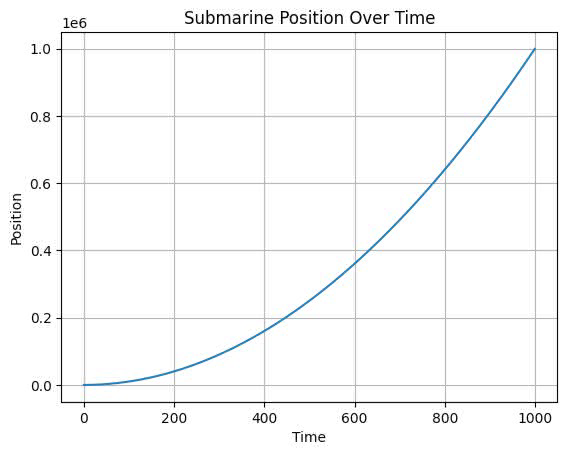
\includegraphics[width=213.75pt,height=171.5pt]{latexImage_b7f75b9b3693005e00d4932fa87a8e27.png}}
\put(269.6,-235.011){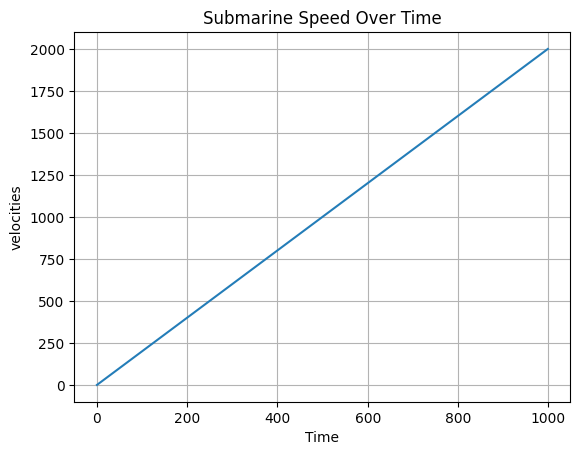
\includegraphics[width=221.15pt,height=173.5pt]{latexImage_0b43c4954eab3d6dd9806f4000802b72.png}}
\put(56,-248.311){\fontsize{11}{1}\usefont{T1}{ptm}{m}{n}\selectfont\color{color_80434} }
\put(58.695,-248.311){\fontsize{11}{1}\usefont{T1}{ptm}{m}{n}\selectfont\color{color_80434} }
\put(61.489,-248.311){\fontsize{11}{1}\usefont{T1}{ptm}{m}{n}\selectfont\color{color_80434} }
\put(64.184,-248.311){\fontsize{11}{1}\usefont{T1}{ptm}{m}{n}\selectfont\color{color_80434} }
\put(66.978,-248.311){\fontsize{11}{1}\usefont{T1}{ptm}{m}{n}\selectfont\color{color_80434} }
\put(69.673,-248.311){\fontsize{11}{1}\usefont{T1}{ptm}{m}{n}\selectfont\color{color_80434} }
\put(72.467,-248.311){\fontsize{11}{1}\usefont{T1}{ptm}{m}{n}\selectfont\color{color_80434} }
\put(75.16199,-248.311){\fontsize{11}{1}\usefont{T1}{ptm}{m}{n}\selectfont\color{color_80434} }
\put(77.95599,-248.311){\fontsize{11}{1}\usefont{T1}{ptm}{m}{n}\selectfont\color{color_80434} }
\put(80.65099,-248.311){\fontsize{11}{1}\usefont{T1}{ptm}{m}{n}\selectfont\color{color_80434} }
\put(83.44499,-248.311){\fontsize{11}{1}\usefont{T1}{ptm}{m}{n}\selectfont\color{color_80434} }
\put(86.13999,-248.311){\fontsize{11}{1}\usefont{T1}{ptm}{m}{n}\selectfont\color{color_80434} }
\put(88.93399,-248.311){\fontsize{11}{1}\usefont{T1}{ptm}{m}{n}\selectfont\color{color_80434} }
\put(91.7,-248.311){\fontsize{11}{1}\usefont{T1}{cmr}{m}{n}\selectfont\color{color_80434}图}
\put(104.9,-248.311){\fontsize{11}{1}\usefont{T1}{ptm}{m}{n}\selectfont\color{color_80434}6.}
\put(223.2,-248.311){\fontsize{11}{1}\usefont{T1}{cmr}{m}{n}\selectfont\color{color_80434}                                 }
\put(113.2,-248.311){\fontsize{11}{1}\usefont{T1}{cmr}{m}{n}\selectfont\color{color_80434}潜水器位置随时间变化}
\put(338.7,-248.311){\fontsize{11}{1}\usefont{T1}{cmr}{m}{n}\selectfont\color{color_80434}图}
\put(351.9,-248.311){\fontsize{11}{1}\usefont{T1}{ptm}{m}{n}\selectfont\color{color_80434}7}
\put(357.301,-248.311){\fontsize{11}{1}\usefont{T1}{ptm}{m}{n}\selectfont\color{color_80434}.}
\put(360.1,-248.311){\fontsize{11}{1}\usefont{T1}{cmr}{m}{n}\selectfont\color{color_80434}潜水器}
\put(393.1,-248.311){\fontsize{11}{1}\usefont{T1}{cmr}{m}{n}\selectfont\color{color_80434}速度}
\put(415.1,-248.311){\fontsize{11}{1}\usefont{T1}{cmr}{m}{n}\selectfont\color{color_80434}随时间变化}
\put(78,-268.911){\fontsize{16}{1}\usefont{T1}{ptm}{b}{n}\selectfont\color{color_55609}5}
\put(86,-268.911){\fontsize{16}{1}\usefont{T1}{cmr}{m}{n}\selectfont\color{color_55609}、}
\put(119,-268.911){\fontsize{16}{1}\usefont{T1}{cmr}{m}{n}\selectfont\color{color_55609}模型的}
\put(167,-268.911){\fontsize{16}{1}\usefont{T1}{cmr}{m}{n}\selectfont\color{color_55609}误差}
\put(199,-268.911){\fontsize{16}{1}\usefont{T1}{cmr}{m}{n}\selectfont\color{color_55609}分析}
\put(56,-316.811){\fontsize{12}{1}\usefont{T1}{cmr}{m}{n}\selectfont\color{color_80434}我}
\put(68,-316.811){\fontsize{12}{1}\usefont{T1}{cmr}{m}{n}\selectfont\color{color_80434}们}
\put(80,-316.811){\fontsize{12}{1}\usefont{T1}{cmr}{m}{n}\selectfont\color{color_80434}采}
\put(92,-316.811){\fontsize{12}{1}\usefont{T1}{cmr}{m}{n}\selectfont\color{color_80434}用的定位模型}
\put(164,-316.811){\fontsize{12}{1}\usefont{T1}{cmr}{m}{n}\selectfont\color{color_80434}是非线}
\put(200,-316.811){\fontsize{12}{1}\usefont{T1}{cmr}{m}{n}\selectfont\color{color_80434}性}
\put(214.4,-316.811){\fontsize{12}{1}\usefont{T1}{ptm}{m}{n}\selectfont\color{color_80434}K}
\put(223.088,-316.811){\fontsize{12}{1}\usefont{T1}{ptm}{m}{n}\selectfont\color{color_80434}a}
\put(228.392,-316.811){\fontsize{12}{1}\usefont{T1}{ptm}{m}{n}\selectfont\color{color_80434}l}
\put(231.692,-316.811){\fontsize{12}{1}\usefont{T1}{ptm}{m}{n}\selectfont\color{color_80434}m}
\put(240.992,-316.811){\fontsize{12}{1}\usefont{T1}{ptm}{m}{n}\selectfont\color{color_80434}a}
\put(246.296,-316.811){\fontsize{12}{1}\usefont{T1}{ptm}{m}{n}\selectfont\color{color_80434}n}
\put(254.8,-316.811){\fontsize{12}{1}\usefont{T1}{cmr}{m}{n}\selectfont\color{color_80434}模型,}
\put(290.8,-316.811){\fontsize{12}{1}\usefont{T1}{cmr}{m}{n}\selectfont\color{color_80434}非线}
\put(314.8,-316.811){\fontsize{12}{1}\usefont{T1}{cmr}{m}{n}\selectfont\color{color_80434}性}
\put(329.2,-316.811){\fontsize{12}{1}\usefont{T1}{ptm}{m}{n}\selectfont\color{color_80434}K}
\put(337.888,-316.811){\fontsize{12}{1}\usefont{T1}{ptm}{m}{n}\selectfont\color{color_80434}a}
\put(343.192,-316.811){\fontsize{12}{1}\usefont{T1}{ptm}{m}{n}\selectfont\color{color_80434}l}
\put(346.492,-316.811){\fontsize{12}{1}\usefont{T1}{ptm}{m}{n}\selectfont\color{color_80434}m}
\put(355.792,-316.811){\fontsize{12}{1}\usefont{T1}{ptm}{m}{n}\selectfont\color{color_80434}a}
\put(361.0959,-316.811){\fontsize{12}{1}\usefont{T1}{ptm}{m}{n}\selectfont\color{color_80434}n}
\put(369.6,-316.811){\fontsize{12}{1}\usefont{T1}{cmr}{m}{n}\selectfont\color{color_80434}模型}
\put(393.6,-316.811){\fontsize{12}{1}\usefont{T1}{cmr}{m}{n}\selectfont\color{color_80434}包括}
\put(420,-316.811){\fontsize{12}{1}\usefont{T1}{ptm}{m}{n}\selectfont\color{color_80434}E}
\put(427.296,-316.811){\fontsize{12}{1}\usefont{T1}{ptm}{m}{n}\selectfont\color{color_80434}K}
\put(435.984,-316.811){\fontsize{12}{1}\usefont{T1}{ptm}{m}{n}\selectfont\color{color_80434}F}
\put(445.1,-316.811){\fontsize{12}{1}\usefont{T1}{cmr}{m}{n}\selectfont\color{color_80434}和}
\put(459.5,-316.811){\fontsize{12}{1}\usefont{T1}{ptm}{m}{n}\selectfont\color{color_80434}U}
\put(468.104,-316.811){\fontsize{12}{1}\usefont{T1}{ptm}{m}{n}\selectfont\color{color_80434}K}
\put(476.792,-316.811){\fontsize{12}{1}\usefont{T1}{ptm}{m}{n}\selectfont\color{color_80434}F}
\put(483.5,-316.811){\fontsize{12}{1}\usefont{T1}{cmr}{m}{n}\selectfont\color{color_80434},}
\put(495.5,-316.811){\fontsize{12}{1}\usefont{T1}{cmr}{m}{n}\selectfont\color{color_80434}其}
\put(56,-330.811){\fontsize{12}{1}\usefont{T1}{cmr}{m}{n}\selectfont\color{color_80434}中}
\put(70.4,-330.811){\fontsize{12}{1}\usefont{T1}{ptm}{m}{n}\selectfont\color{color_80434}E}
\put(77.696,-330.811){\fontsize{12}{1}\usefont{T1}{ptm}{m}{n}\selectfont\color{color_80434}K}
\put(86.384,-330.811){\fontsize{12}{1}\usefont{T1}{ptm}{m}{n}\selectfont\color{color_80434}F}
\put(95.5,-330.811){\fontsize{12}{1}\usefont{T1}{cmr}{m}{n}\selectfont\color{color_80434}广泛}
\put(119.5,-330.811){\fontsize{12}{1}\usefont{T1}{cmr}{m}{n}\selectfont\color{color_80434}应用于个}
\put(167.5,-330.811){\fontsize{12}{1}\usefont{T1}{cmr}{m}{n}\selectfont\color{color_80434}领}
\put(179.5,-330.811){\fontsize{12}{1}\usefont{T1}{cmr}{m}{n}\selectfont\color{color_80434}域}
\put(191.5,-330.811){\fontsize{12}{1}\usefont{T1}{ptm}{m}{n}\selectfont\color{color_80434}.}
\put(194.5,-330.811){\fontsize{12}{1}\usefont{T1}{cmr}{m}{n}\selectfont\color{color_80434}其}
\put(206.5,-330.811){\fontsize{12}{1}\usefont{T1}{cmr}{m}{n}\selectfont\color{color_80434}基本}
\put(230.5,-330.811){\fontsize{12}{1}\usefont{T1}{cmr}{m}{n}\selectfont\color{color_80434}原}
\put(242.5,-330.811){\fontsize{12}{1}\usefont{T1}{cmr}{m}{n}\selectfont\color{color_80434}理}
\put(254.5,-330.811){\fontsize{12}{1}\usefont{T1}{cmr}{m}{n}\selectfont\color{color_80434}是}
\put(266.5,-330.811){\fontsize{12}{1}\usefont{T1}{cmr}{m}{n}\selectfont\color{color_80434}用系}
\put(290.5,-330.811){\fontsize{12}{1}\usefont{T1}{cmr}{m}{n}\selectfont\color{color_80434}统}
\put(302.5,-330.811){\fontsize{12}{1}\usefont{T1}{cmr}{m}{n}\selectfont\color{color_80434}观测}
\put(326.5,-330.811){\fontsize{12}{1}\usefont{T1}{cmr}{m}{n}\selectfont\color{color_80434}值来修正}
\put(374.5,-330.811){\fontsize{12}{1}\usefont{T1}{cmr}{m}{n}\selectfont\color{color_80434}系}
\put(386.5,-330.811){\fontsize{12}{1}\usefont{T1}{cmr}{m}{n}\selectfont\color{color_80434}统状}
\put(410.5,-330.811){\fontsize{12}{1}\usefont{T1}{cmr}{m}{n}\selectfont\color{color_80434}态,}
\put(434.5,-330.811){\fontsize{12}{1}\usefont{T1}{cmr}{m}{n}\selectfont\color{color_80434}直}
\put(446.5,-330.811){\fontsize{12}{1}\usefont{T1}{cmr}{m}{n}\selectfont\color{color_80434}到系}
\put(470.5,-330.811){\fontsize{12}{1}\usefont{T1}{cmr}{m}{n}\selectfont\color{color_80434}统误差}
\put(56,-344.911){\fontsize{12}{1}\usefont{T1}{cmr}{m}{n}\selectfont\color{color_80434}无限接近}
\put(104,-344.911){\fontsize{12}{1}\usefont{T1}{cmr}{m}{n}\selectfont\color{color_80434}于}
\put(118.4,-344.911){\fontsize{12}{1}\usefont{T1}{ptm}{m}{n}\selectfont\color{color_80434}Cra}
\put(135.692,-344.911){\fontsize{12}{1}\usefont{T1}{ptm}{m}{n}\selectfont\color{color_80434}m}
\put(144.992,-344.911){\fontsize{12}{1}\usefont{T1}{ptm}{m}{n}\selectfont\color{color_80434}e}
\put(150.296,-344.911){\fontsize{12}{1}\usefont{T1}{ptm}{m}{n}\selectfont\color{color_80434}r}
\put(154.1,-344.911){\fontsize{12}{1}\usefont{T1}{ptm}{m}{n}\selectfont\color{color_80434}-Ra}
\put(171.392,-344.911){\fontsize{12}{1}\usefont{T1}{ptm}{m}{n}\selectfont\color{color_80434}o}
\put(179.8,-344.911){\fontsize{12}{1}\usefont{T1}{cmr}{m}{n}\selectfont\color{color_80434}下}
\put(191.8,-344.911){\fontsize{12}{1}\usefont{T1}{cmr}{m}{n}\selectfont\color{color_80434}界;}
\put(215.8,-344.911){\fontsize{12}{1}\usefont{T1}{ptm}{m}{n}\selectfont\color{color_80434}U}
\put(224.488,-344.911){\fontsize{12}{1}\usefont{T1}{ptm}{m}{n}\selectfont\color{color_80434}K}
\put(233.092,-344.911){\fontsize{12}{1}\usefont{T1}{ptm}{m}{n}\selectfont\color{color_80434}F}
\put(242.2,-344.911){\fontsize{12}{1}\usefont{T1}{cmr}{m}{n}\selectfont\color{color_80434}是}
\put(254.2,-344.911){\fontsize{12}{1}\usefont{T1}{cmr}{m}{n}\selectfont\color{color_80434}针}
\put(266.2,-344.911){\fontsize{12}{1}\usefont{T1}{cmr}{m}{n}\selectfont\color{color_80434}对}
\put(278.2,-344.911){\fontsize{12}{1}\usefont{T1}{cmr}{m}{n}\selectfont\color{color_80434}强}
\put(290.2,-344.911){\fontsize{12}{1}\usefont{T1}{cmr}{m}{n}\selectfont\color{color_80434}非线}
\put(314.2,-344.911){\fontsize{12}{1}\usefont{T1}{cmr}{m}{n}\selectfont\color{color_80434}性系}
\put(338.2,-344.911){\fontsize{12}{1}\usefont{T1}{cmr}{m}{n}\selectfont\color{color_80434}统}
\put(350.2,-344.911){\fontsize{12}{1}\usefont{T1}{cmr}{m}{n}\selectfont\color{color_80434}提出的一}
\put(398.2,-344.911){\fontsize{12}{1}\usefont{T1}{cmr}{m}{n}\selectfont\color{color_80434}种}
\put(410.2,-344.911){\fontsize{12}{1}\usefont{T1}{cmr}{m}{n}\selectfont\color{color_80434}采}
\put(422.2,-344.911){\fontsize{12}{1}\usefont{T1}{cmr}{m}{n}\selectfont\color{color_80434}用多}
\put(446.2,-344.911){\fontsize{12}{1}\usefont{T1}{cmr}{m}{n}\selectfont\color{color_80434}粒子逼}
\put(482.2,-344.911){\fontsize{12}{1}\usefont{T1}{cmr}{m}{n}\selectfont\color{color_80434}近}
\put(494.2,-344.911){\fontsize{12}{1}\usefont{T1}{cmr}{m}{n}\selectfont\color{color_80434}函}
\put(56,-358.911){\fontsize{12}{1}\usefont{T1}{cmr}{m}{n}\selectfont\color{color_80434}数的概率}
\put(104,-358.911){\fontsize{12}{1}\usefont{T1}{cmr}{m}{n}\selectfont\color{color_80434}密度}
\put(128,-358.911){\fontsize{12}{1}\usefont{T1}{cmr}{m}{n}\selectfont\color{color_80434}分布的方式}
\put(188,-358.911){\fontsize{12}{1}\usefont{T1}{cmr}{m}{n}\selectfont\color{color_80434}获}
\put(200,-358.911){\fontsize{12}{1}\usefont{T1}{cmr}{m}{n}\selectfont\color{color_80434}得更高}
\put(236,-358.911){\fontsize{12}{1}\usefont{T1}{cmr}{m}{n}\selectfont\color{color_80434}阶}
\put(248,-358.911){\fontsize{12}{1}\usefont{T1}{cmr}{m}{n}\selectfont\color{color_80434}次}
\put(260,-358.911){\fontsize{12}{1}\usefont{T1}{cmr}{m}{n}\selectfont\color{color_80434}的}
\put(272,-358.911){\fontsize{12}{1}\usefont{T1}{cmr}{m}{n}\selectfont\color{color_80434}均值}
\put(296,-358.911){\fontsize{12}{1}\usefont{T1}{cmr}{m}{n}\selectfont\color{color_80434}和方}
\put(320,-358.911){\fontsize{12}{1}\usefont{T1}{cmr}{m}{n}\selectfont\color{color_80434}差}
\put(332,-358.911){\fontsize{12}{1}\usefont{T1}{cmr}{m}{n}\selectfont\color{color_80434},}
\put(344,-358.911){\fontsize{12}{1}\usefont{T1}{cmr}{m}{n}\selectfont\color{color_80434}我}
\put(356,-358.911){\fontsize{12}{1}\usefont{T1}{cmr}{m}{n}\selectfont\color{color_80434}们的定位模型}
\put(428,-358.911){\fontsize{12}{1}\usefont{T1}{cmr}{m}{n}\selectfont\color{color_80434}适}
\put(440,-358.911){\fontsize{12}{1}\usefont{T1}{cmr}{m}{n}\selectfont\color{color_80434}合}
\put(452,-358.911){\fontsize{12}{1}\usefont{T1}{cmr}{m}{n}\selectfont\color{color_80434}采}
\put(464,-358.911){\fontsize{12}{1}\usefont{T1}{cmr}{m}{n}\selectfont\color{color_80434}用}
\put(478.4,-358.911){\fontsize{12}{1}\usefont{T1}{ptm}{m}{n}\selectfont\color{color_80434}E}
\put(485.696,-358.911){\fontsize{12}{1}\usefont{T1}{ptm}{m}{n}\selectfont\color{color_80434}K}
\put(494.384,-358.911){\fontsize{12}{1}\usefont{T1}{ptm}{m}{n}\selectfont\color{color_80434}F}
\put(500.084,-358.911){\fontsize{12}{1}\usefont{T1}{ptm}{m}{n}\selectfont\color{color_80434}.}
\end{picture}
\begin{tikzpicture}[overlay]
\path(0pt,0pt);
\filldraw[color_283006][even odd rule]
(55.9pt, -399.661pt) -- (78.75pt, -399.661pt)
 -- (78.75pt, -399.661pt)
 -- (78.75pt, -381.611pt)
 -- (78.75pt, -381.611pt)
 -- (55.9pt, -381.611pt) -- cycle
;
\end{tikzpicture}
\begin{picture}(-5,0)(2.5,0)
\put(56,-396.011){\fontsize{15.5}{1}\usefont{T1}{ptm}{b}{n}\selectfont\color{color_54684}a}
\put(66.4005,-396.011){\fontsize{15.5}{1}\usefont{T1}{ptm}{b}{n}\selectfont\color{color_54684}) }
\end{picture}
\begin{tikzpicture}[overlay]
\path(0pt,0pt);
\filldraw[color_283006][even odd rule]
(78.8pt, -399.661pt) -- (357.75pt, -399.661pt)
 -- (357.75pt, -399.661pt)
 -- (357.75pt, -381.611pt)
 -- (357.75pt, -381.611pt)
 -- (78.8pt, -381.611pt) -- cycle
;
\end{tikzpicture}
\begin{picture}(-5,0)(2.5,0)
\put(78.9,-396.011){\fontsize{15.5}{1}\usefont{T1}{cmr}{m}{n}\selectfont\color{color_54684}最优}
\put(109.9,-396.011){\fontsize{15.5}{1}\usefont{T1}{cmr}{m}{n}\selectfont\color{color_54684}估}
\put(125.4,-396.011){\fontsize{15.5}{1}\usefont{T1}{cmr}{m}{n}\selectfont\color{color_54684}计}
\put(140.9,-396.011){\fontsize{15.5}{1}\usefont{T1}{cmr}{m}{n}\selectfont\color{color_54684}值}
\put(156.4,-396.011){\fontsize{15.5}{1}\usefont{T1}{cmr}{m}{n}\selectfont\color{color_54684}和预测}
\put(202.9,-396.011){\fontsize{15.5}{1}\usefont{T1}{cmr}{m}{n}\selectfont\color{color_54684}值}
\put(218.4,-396.011){\fontsize{15.5}{1}\usefont{T1}{cmr}{m}{n}\selectfont\color{color_54684}、观测}
\put(264.9,-396.011){\fontsize{15.5}{1}\usefont{T1}{cmr}{m}{n}\selectfont\color{color_54684}值}
\put(280.4,-396.011){\fontsize{15.5}{1}\usefont{T1}{cmr}{m}{n}\selectfont\color{color_54684}的关系推}
\put(342.4,-396.011){\fontsize{15.5}{1}\usefont{T1}{cmr}{m}{n}\selectfont\color{color_54684}导}
\put(56,-414.211){\fontsize{11}{1}\usefont{T1}{cmr}{m}{n}\selectfont\color{color_80434}为了更}
\put(89,-414.211){\fontsize{11}{1}\usefont{T1}{cmr}{m}{n}\selectfont\color{color_80434}好}
\put(100,-414.211){\fontsize{11}{1}\usefont{T1}{cmr}{m}{n}\selectfont\color{color_80434}地预测潜水器的定位,}
\put(210,-414.211){\fontsize{11}{1}\usefont{T1}{cmr}{m}{n}\selectfont\color{color_80434}我}
\put(221,-414.211){\fontsize{11}{1}\usefont{T1}{cmr}{m}{n}\selectfont\color{color_80434}们}
\put(232,-414.211){\fontsize{11}{1}\usefont{T1}{cmr}{m}{n}\selectfont\color{color_80434}继续}
\put(254,-414.211){\fontsize{11}{1}\usefont{T1}{cmr}{m}{n}\selectfont\color{color_80434}使用}
\put(278.2,-414.211){\fontsize{11}{1}\usefont{T1}{ptm}{m}{n}\selectfont\color{color_80434}E}
\put(284.899,-414.211){\fontsize{11}{1}\usefont{T1}{ptm}{m}{n}\selectfont\color{color_80434}K}
\put(292.797,-414.211){\fontsize{11}{1}\usefont{T1}{ptm}{m}{n}\selectfont\color{color_80434}F}
\put(301.2,-414.211){\fontsize{11}{1}\usefont{T1}{cmr}{m}{n}\selectfont\color{color_80434}模型进行加}
\put(356.2,-414.211){\fontsize{11}{1}\usefont{T1}{cmr}{m}{n}\selectfont\color{color_80434}强}
\put(367.2,-414.211){\fontsize{11}{1}\usefont{T1}{cmr}{m}{n}\selectfont\color{color_80434},}
\put(378.2,-414.211){\fontsize{11}{1}\usefont{T1}{cmr}{m}{n}\selectfont\color{color_80434}我}
\put(389.2,-414.211){\fontsize{11}{1}\usefont{T1}{cmr}{m}{n}\selectfont\color{color_80434}们给出:}
\put(350.3,-447.511){\fontsize{11}{1}\usefont{T1}{ptm}{m}{n}\selectfont\color{color_80434} }
\put(353.094,-447.511){\fontsize{11}{1}\usefont{T1}{ptm}{m}{n}\selectfont\color{color_80434} }
\put(355.789,-447.511){\fontsize{11}{1}\usefont{T1}{ptm}{m}{n}\selectfont\color{color_80434} }
\put(358.583,-447.511){\fontsize{11}{1}\usefont{T1}{ptm}{m}{n}\selectfont\color{color_80434} }
\put(361.278,-447.511){\fontsize{11}{1}\usefont{T1}{ptm}{m}{n}\selectfont\color{color_80434} }
\put(364.072,-447.511){\fontsize{11}{1}\usefont{T1}{ptm}{m}{n}\selectfont\color{color_80434} }
\put(366.767,-447.511){\fontsize{11}{1}\usefont{T1}{ptm}{m}{n}\selectfont\color{color_80434} }
\put(369.561,-447.511){\fontsize{11}{1}\usefont{T1}{ptm}{m}{n}\selectfont\color{color_80434} }
\put(372.256,-447.511){\fontsize{11}{1}\usefont{T1}{ptm}{m}{n}\selectfont\color{color_80434} }
\put(375.05,-447.511){\fontsize{11}{1}\usefont{T1}{ptm}{m}{n}\selectfont\color{color_80434} }
\put(377.7451,-447.511){\fontsize{11}{1}\usefont{T1}{ptm}{m}{n}\selectfont\color{color_80434} }
\put(324.8,-478.011){\fontsize{11}{1}\usefont{T1}{ptm}{m}{n}\selectfont\color{color_80434} }
\put(327.594,-478.011){\fontsize{11}{1}\usefont{T1}{ptm}{m}{n}\selectfont\color{color_80434} }
\put(330.289,-478.011){\fontsize{11}{1}\usefont{T1}{ptm}{m}{n}\selectfont\color{color_80434} }
\put(333.083,-478.011){\fontsize{11}{1}\usefont{T1}{ptm}{m}{n}\selectfont\color{color_80434} }
\put(335.778,-478.011){\fontsize{11}{1}\usefont{T1}{ptm}{m}{n}\selectfont\color{color_80434} }
\put(338.572,-478.011){\fontsize{11}{1}\usefont{T1}{ptm}{m}{n}\selectfont\color{color_80434} }
\put(341.267,-478.011){\fontsize{11}{1}\usefont{T1}{ptm}{m}{n}\selectfont\color{color_80434} }
\put(344.061,-478.011){\fontsize{11}{1}\usefont{T1}{ptm}{m}{n}\selectfont\color{color_80434} }
\put(346.756,-478.011){\fontsize{11}{1}\usefont{T1}{ptm}{m}{n}\selectfont\color{color_80434} }
\put(349.55,-478.011){\fontsize{11}{1}\usefont{T1}{ptm}{m}{n}\selectfont\color{color_80434} }
\put(352.2451,-478.011){\fontsize{11}{1}\usefont{T1}{ptm}{m}{n}\selectfont\color{color_80434} }
\put(355.0391,-478.011){\fontsize{11}{1}\usefont{T1}{ptm}{m}{n}\selectfont\color{color_80434} }
\put(357.7341,-478.011){\fontsize{11}{1}\usefont{T1}{ptm}{m}{n}\selectfont\color{color_80434} }
\put(360.5281,-478.011){\fontsize{11}{1}\usefont{T1}{ptm}{m}{n}\selectfont\color{color_80434} }
\put(363.2231,-478.011){\fontsize{11}{1}\usefont{T1}{ptm}{m}{n}\selectfont\color{color_80434} }
\put(366.0171,-478.011){\fontsize{11}{1}\usefont{T1}{ptm}{m}{n}\selectfont\color{color_80434} }
\put(368.7121,-478.011){\fontsize{11}{1}\usefont{T1}{ptm}{m}{n}\selectfont\color{color_80434} }
\put(176,-517.611){\fontsize{10}{1}\usefont{T1}{cmr}{m}{n}\selectfont\color{color_80434} }
\put(179.19,-517.611){\fontsize{10}{1}\usefont{T1}{cmr}{m}{n}\selectfont\color{color_80434} }
\put(56,-517.611){\fontsize{10}{1}\usefont{T1}{cmr}{m}{n}\selectfont\color{color_80434}从}
\put(66,-517.611){\fontsize{10}{1}\usefont{T1}{cmr}{m}{n}\selectfont\color{color_80434}观测}
\put(86,-517.611){\fontsize{10}{1}\usefont{T1}{cmr}{m}{n}\selectfont\color{color_80434}角度}
\put(106,-517.611){\fontsize{10}{1}\usefont{T1}{cmr}{m}{n}\selectfont\color{color_80434}出发,对于}
\put(156,-517.611){\fontsize{10}{1}\usefont{T1}{cmr}{m}{n}\selectfont\color{color_80434}公}
\put(166,-517.611){\fontsize{10}{1}\usefont{T1}{cmr}{m}{n}\selectfont\color{color_80434}式}
\put(266.4,-517.611){\fontsize{10}{1}\usefont{T1}{cmr}{m}{n}\selectfont\color{color_80434}:}
\put(56,-537.111){\fontsize{10}{1}\usefont{T1}{cmr}{m}{n}\selectfont\color{color_80434}我}
\put(66,-537.111){\fontsize{10}{1}\usefont{T1}{cmr}{m}{n}\selectfont\color{color_80434}们}
\put(76,-537.111){\fontsize{10}{1}\usefont{T1}{cmr}{m}{n}\selectfont\color{color_80434}忽略}
\put(96,-537.111){\fontsize{10}{1}\usefont{T1}{cmr}{m}{n}\selectfont\color{color_80434}掉}
\put(106,-537.111){\fontsize{10}{1}\usefont{T1}{cmr}{m}{n}\selectfont\color{color_80434}观测}
\put(126,-537.111){\fontsize{10}{1}\usefont{T1}{cmr}{m}{n}\selectfont\color{color_80434}噪}
\put(136,-537.111){\fontsize{10}{1}\usefont{T1}{cmr}{m}{n}\selectfont\color{color_80434}声}
\put(158,-537.111){\fontsize{10}{1}\usefont{T1}{cmr}{m}{n}\selectfont\color{color_80434},用}
\put(190.8,-537.111){\fontsize{10}{1}\usefont{T1}{cmr}{m}{n}\selectfont\color{color_80434}替代}
\put(210.8,-537.111){\fontsize{10}{1}\usefont{T1}{cmr}{m}{n}\selectfont\color{color_80434}真}
\put(220.8,-537.111){\fontsize{10}{1}\usefont{T1}{cmr}{m}{n}\selectfont\color{color_80434}实值}
\put(240.8,-537.111){\fontsize{10}{1}\usefont{T1}{cmr}{m}{n}\selectfont\color{color_80434},得到}
\put(56,-580.211){\fontsize{10}{1}\usefont{T1}{cmr}{m}{n}\selectfont\color{color_80434}我}
\put(66,-580.211){\fontsize{10}{1}\usefont{T1}{cmr}{m}{n}\selectfont\color{color_80434}们通过预测}
\put(116,-580.211){\fontsize{10}{1}\usefont{T1}{cmr}{m}{n}\selectfont\color{color_80434}值}
\put(126,-580.211){\fontsize{10}{1}\usefont{T1}{cmr}{m}{n}\selectfont\color{color_80434}和观测}
\put(156,-580.211){\fontsize{10}{1}\usefont{T1}{cmr}{m}{n}\selectfont\color{color_80434}矩阵}
\put(176,-580.211){\fontsize{10}{1}\usefont{T1}{cmr}{m}{n}\selectfont\color{color_80434}获}
\put(186,-580.211){\fontsize{10}{1}\usefont{T1}{cmr}{m}{n}\selectfont\color{color_80434}得了和测}
\put(226,-580.211){\fontsize{10}{1}\usefont{T1}{cmr}{m}{n}\selectfont\color{color_80434}量值}
\put(246,-580.211){\fontsize{10}{1}\usefont{T1}{cmr}{m}{n}\selectfont\color{color_80434}相同维}
\put(276,-580.211){\fontsize{10}{1}\usefont{T1}{cmr}{m}{n}\selectfont\color{color_80434}度}
\put(286,-580.211){\fontsize{10}{1}\usefont{T1}{cmr}{m}{n}\selectfont\color{color_80434}的}
\put(339.5,-580.211){\fontsize{10}{1}\usefont{T1}{cmr}{m}{n}\selectfont\color{color_80434},用}
\put(359.5,-580.211){\fontsize{10}{1}\usefont{T1}{cmr}{m}{n}\selectfont\color{color_80434}来}
\put(369.5,-580.211){\fontsize{10}{1}\usefont{T1}{cmr}{m}{n}\selectfont\color{color_80434}和观测}
\put(399.5,-580.211){\fontsize{10}{1}\usefont{T1}{cmr}{m}{n}\selectfont\color{color_80434}值}
\put(409.5,-580.211){\fontsize{10}{1}\usefont{T1}{cmr}{m}{n}\selectfont\color{color_80434}的}
\put(419.5,-580.211){\fontsize{10}{1}\usefont{T1}{cmr}{m}{n}\selectfont\color{color_80434}误差}
\put(439.5,-580.211){\fontsize{10}{1}\usefont{T1}{cmr}{m}{n}\selectfont\color{color_80434}项}
\put(449.5,-580.211){\fontsize{10}{1}\usefont{T1}{cmr}{m}{n}\selectfont\color{color_80434}来修正}
\put(479.5,-580.211){\fontsize{10}{1}\usefont{T1}{cmr}{m}{n}\selectfont\color{color_80434}预测}
\put(499.5,-580.211){\fontsize{10}{1}\usefont{T1}{cmr}{m}{n}\selectfont\color{color_80434}值}
\put(509.5,-580.211){\fontsize{10}{1}\usefont{T1}{cmr}{m}{n}\selectfont\color{color_80434},}
\put(56,-598.611){\fontsize{10}{1}\usefont{T1}{cmr}{m}{n}\selectfont\color{color_80434}考虑}
\put(76,-598.611){\fontsize{10}{1}\usefont{T1}{cmr}{m}{n}\selectfont\color{color_80434}到维}
\put(96,-598.611){\fontsize{10}{1}\usefont{T1}{cmr}{m}{n}\selectfont\color{color_80434}度}
\put(106,-598.611){\fontsize{10}{1}\usefont{T1}{cmr}{m}{n}\selectfont\color{color_80434}可能不同等因素,}
\put(186,-598.611){\fontsize{10}{1}\usefont{T1}{cmr}{m}{n}\selectfont\color{color_80434}我}
\put(196,-598.611){\fontsize{10}{1}\usefont{T1}{cmr}{m}{n}\selectfont\color{color_80434}们用系数}
\put(236,-598.611){\fontsize{10}{1}\usefont{T1}{cmr}{m}{n}\selectfont\color{color_80434}矩阵}
\put(268,-598.611){\fontsize{10}{1}\usefont{T1}{cmr}{m}{n}\selectfont\color{color_80434}进行}
\put(288,-598.611){\fontsize{10}{1}\usefont{T1}{cmr}{m}{n}\selectfont\color{color_80434}修正}
\put(56,-660.111){\fontsize{10}{1}\usefont{T1}{cmr}{m}{n}\selectfont\color{color_80434}所}
\put(66,-660.111){\fontsize{10}{1}\usefont{T1}{cmr}{m}{n}\selectfont\color{color_80434}以}
\put(76,-660.111){\fontsize{10}{1}\usefont{T1}{cmr}{m}{n}\selectfont\color{color_80434}只}
\put(86,-660.111){\fontsize{10}{1}\usefont{T1}{cmr}{m}{n}\selectfont\color{color_80434}要}
\put(96,-660.111){\fontsize{10}{1}\usefont{T1}{cmr}{m}{n}\selectfont\color{color_80434}我}
\put(106,-660.111){\fontsize{10}{1}\usefont{T1}{cmr}{m}{n}\selectfont\color{color_80434}们找到一个合}
\put(166,-660.111){\fontsize{10}{1}\usefont{T1}{cmr}{m}{n}\selectfont\color{color_80434}适}
\put(176,-660.111){\fontsize{10}{1}\usefont{T1}{cmr}{m}{n}\selectfont\color{color_80434}的}
\put(198,-660.111){\fontsize{10}{1}\usefont{T1}{cmr}{m}{n}\selectfont\color{color_80434}值}
\put(208,-660.111){\fontsize{10}{1}\usefont{T1}{cmr}{m}{n}\selectfont\color{color_80434},使得最优}
\put(258,-660.111){\fontsize{10}{1}\usefont{T1}{cmr}{m}{n}\selectfont\color{color_80434}估}
\put(268,-660.111){\fontsize{10}{1}\usefont{T1}{cmr}{m}{n}\selectfont\color{color_80434}计}
\put(278,-660.111){\fontsize{10}{1}\usefont{T1}{cmr}{m}{n}\selectfont\color{color_80434}值接近}
\put(308,-660.111){\fontsize{10}{1}\usefont{T1}{cmr}{m}{n}\selectfont\color{color_80434}真}
\put(318,-660.111){\fontsize{10}{1}\usefont{T1}{cmr}{m}{n}\selectfont\color{color_80434}实值}
\put(56,-681.611){\fontsize{10}{1}\usefont{T1}{cmr}{m}{n}\selectfont\color{color_80434}我}
\put(66,-681.611){\fontsize{10}{1}\usefont{T1}{cmr}{m}{n}\selectfont\color{color_80434}们}
\put(76,-681.611){\fontsize{10}{1}\usefont{T1}{cmr}{m}{n}\selectfont\color{color_80434}假}
\put(86,-681.611){\fontsize{10}{1}\usefont{T1}{cmr}{m}{n}\selectfont\color{color_80434}设}
\put(169.5,-681.611){\fontsize{10}{1}\usefont{T1}{cmr}{m}{n}\selectfont\color{color_80434},和}
\put(189.5,-681.611){\fontsize{10}{1}\usefont{T1}{cmr}{m}{n}\selectfont\color{color_80434}公}
\put(199.5,-681.611){\fontsize{10}{1}\usefont{T1}{cmr}{m}{n}\selectfont\color{color_80434}式}
\put(293.6,-681.611){\fontsize{10}{1}\usefont{T1}{cmr}{m}{n}\selectfont\color{color_80434}结合可以得到}
\put(56,-742.111){\fontsize{10}{1}\usefont{T1}{cmr}{m}{n}\selectfont\color{color_80434}继续}
\put(76,-742.111){\fontsize{10}{1}\usefont{T1}{cmr}{m}{n}\selectfont\color{color_80434}假}
\put(86,-742.111){\fontsize{10}{1}\usefont{T1}{cmr}{m}{n}\selectfont\color{color_80434}设}
\put(96,-742.111){\fontsize{10}{1}\usefont{T1}{ptm}{m}{n}\selectfont\color{color_80434}:}
\end{picture}
\newpage
\begin{tikzpicture}[overlay]
\path(0pt,0pt);
\filldraw[color_283006][even odd rule]
(130.2pt, -80.76099pt) -- (133.95pt, -80.76099pt)
 -- (133.95pt, -80.76099pt)
 -- (133.95pt, -66.81097pt)
 -- (133.95pt, -66.81097pt)
 -- (130.2pt, -66.81097pt) -- cycle
;
\end{tikzpicture}
\begin{picture}(-5,0)(2.5,0)
\put(130.3,-77.91101){\fontsize{12}{1}\usefont{T1}{cmr}{m}{n}\selectfont\color{color_54684},}
\end{picture}
\begin{tikzpicture}[overlay]
\path(0pt,0pt);
\filldraw[color_283006][even odd rule]
(134pt, -80.76099pt) -- (385.95pt, -80.76099pt)
 -- (385.95pt, -80.76099pt)
 -- (385.95pt, -66.81097pt)
 -- (385.95pt, -66.81097pt)
 -- (134pt, -66.81097pt) -- cycle
;
\end{tikzpicture}
\begin{picture}(-5,0)(2.5,0)
\put(134.1,-77.91101){\fontsize{12}{1}\usefont{T1}{cmr}{m}{n}\selectfont\color{color_54684}表}
\put(146.1,-77.91101){\fontsize{12}{1}\usefont{T1}{cmr}{m}{n}\selectfont\color{color_54684}示}
\put(158.1,-77.91101){\fontsize{12}{1}\usefont{T1}{cmr}{m}{n}\selectfont\color{color_54684}的}
\put(170.1,-77.91101){\fontsize{12}{1}\usefont{T1}{cmr}{m}{n}\selectfont\color{color_54684}是}
\put(182.1,-77.91101){\fontsize{12}{1}\usefont{T1}{cmr}{m}{n}\selectfont\color{color_54684}真}
\put(194.1,-77.91101){\fontsize{12}{1}\usefont{T1}{cmr}{m}{n}\selectfont\color{color_54684}实值}
\put(218.1,-77.91101){\fontsize{12}{1}\usefont{T1}{cmr}{m}{n}\selectfont\color{color_54684}和最优}
\put(254.1,-77.91101){\fontsize{12}{1}\usefont{T1}{cmr}{m}{n}\selectfont\color{color_54684}值}
\put(266.1,-77.91101){\fontsize{12}{1}\usefont{T1}{cmr}{m}{n}\selectfont\color{color_54684}的后验}
\put(302.1,-77.91101){\fontsize{12}{1}\usefont{T1}{cmr}{m}{n}\selectfont\color{color_54684}误差}
\put(326.1,-77.91101){\fontsize{12}{1}\usefont{T1}{cmr}{m}{n}\selectfont\color{color_54684}协}
\put(338.1,-77.91101){\fontsize{12}{1}\usefont{T1}{cmr}{m}{n}\selectfont\color{color_54684}方}
\put(350.1,-77.91101){\fontsize{12}{1}\usefont{T1}{cmr}{m}{n}\selectfont\color{color_54684}差矩阵}
\end{picture}
\begin{tikzpicture}[overlay]
\path(0pt,0pt);
\filldraw[color_283006][even odd rule]
(142.9pt, -101.561pt) -- (146.65pt, -101.561pt)
 -- (146.65pt, -101.561pt)
 -- (146.65pt, -87.61096pt)
 -- (146.65pt, -87.61096pt)
 -- (142.9pt, -87.61096pt) -- cycle
;
\end{tikzpicture}
\begin{picture}(-5,0)(2.5,0)
\put(143,-98.81097){\fontsize{12}{1}\usefont{T1}{cmr}{m}{n}\selectfont\color{color_54684},}
\end{picture}
\begin{tikzpicture}[overlay]
\path(0pt,0pt);
\filldraw[color_283006][even odd rule]
(146.7pt, -101.561pt) -- (398.65pt, -101.561pt)
 -- (398.65pt, -101.561pt)
 -- (398.65pt, -87.61096pt)
 -- (398.65pt, -87.61096pt)
 -- (146.7pt, -87.61096pt) -- cycle
;
\end{tikzpicture}
\begin{picture}(-5,0)(2.5,0)
\put(146.8,-98.81097){\fontsize{12}{1}\usefont{T1}{cmr}{m}{n}\selectfont\color{color_54684}表}
\put(158.8,-98.81097){\fontsize{12}{1}\usefont{T1}{cmr}{m}{n}\selectfont\color{color_54684}示}
\put(170.8,-98.81097){\fontsize{12}{1}\usefont{T1}{cmr}{m}{n}\selectfont\color{color_54684}的}
\put(182.8,-98.81097){\fontsize{12}{1}\usefont{T1}{cmr}{m}{n}\selectfont\color{color_54684}是}
\put(194.8,-98.81097){\fontsize{12}{1}\usefont{T1}{cmr}{m}{n}\selectfont\color{color_54684}真}
\put(206.8,-98.81097){\fontsize{12}{1}\usefont{T1}{cmr}{m}{n}\selectfont\color{color_54684}实值}
\put(230.8,-98.81097){\fontsize{12}{1}\usefont{T1}{cmr}{m}{n}\selectfont\color{color_54684}和预测}
\put(266.8,-98.81097){\fontsize{12}{1}\usefont{T1}{cmr}{m}{n}\selectfont\color{color_54684}值}
\put(278.8,-98.81097){\fontsize{12}{1}\usefont{T1}{cmr}{m}{n}\selectfont\color{color_54684}的先验}
\put(314.8,-98.81097){\fontsize{12}{1}\usefont{T1}{cmr}{m}{n}\selectfont\color{color_54684}误差}
\put(338.8,-98.81097){\fontsize{12}{1}\usefont{T1}{cmr}{m}{n}\selectfont\color{color_54684}协}
\put(350.8,-98.81097){\fontsize{12}{1}\usefont{T1}{cmr}{m}{n}\selectfont\color{color_54684}方}
\put(362.8,-98.81097){\fontsize{12}{1}\usefont{T1}{cmr}{m}{n}\selectfont\color{color_54684}差矩阵}
\end{picture}
\begin{tikzpicture}[overlay]
\path(0pt,0pt);
\filldraw[color_283006][even odd rule]
(55.9pt, -119.761pt) -- (199.85pt, -119.761pt)
 -- (199.85pt, -119.761pt)
 -- (199.85pt, -105.811pt)
 -- (199.85pt, -105.811pt)
 -- (55.9pt, -105.811pt) -- cycle
;
\end{tikzpicture}
\begin{picture}(-5,0)(2.5,0)
\put(56,-117.011){\fontsize{12}{1}\usefont{T1}{cmr}{m}{n}\selectfont\color{color_54684}根据上}
\put(92,-117.011){\fontsize{12}{1}\usefont{T1}{cmr}{m}{n}\selectfont\color{color_54684}述假}
\put(116,-117.011){\fontsize{12}{1}\usefont{T1}{cmr}{m}{n}\selectfont\color{color_54684}设,}
\put(140,-117.011){\fontsize{12}{1}\usefont{T1}{cmr}{m}{n}\selectfont\color{color_54684}我}
\put(152,-117.011){\fontsize{12}{1}\usefont{T1}{cmr}{m}{n}\selectfont\color{color_54684}们}
\put(164,-117.011){\fontsize{12}{1}\usefont{T1}{cmr}{m}{n}\selectfont\color{color_54684}来求解}
\end{picture}
\begin{tikzpicture}[overlay]
\path(0pt,0pt);
\filldraw[color_283006][even odd rule]
(199.9pt, -119.761pt) -- (202.25pt, -119.761pt)
 -- (202.25pt, -119.761pt)
 -- (202.25pt, -105.811pt)
 -- (202.25pt, -105.811pt)
 -- (199.9pt, -105.811pt) -- cycle
;
\filldraw[color_283006][even odd rule]
(202.3pt, -119.761pt) -- (247.25pt, -119.761pt)
 -- (247.25pt, -119.761pt)
 -- (247.25pt, -105.811pt)
 -- (247.25pt, -105.811pt)
 -- (202.3pt, -105.811pt) -- cycle
;
\end{tikzpicture}
\begin{picture}(-5,0)(2.5,0)
\put(202.4,-117.011){\fontsize{12}{1}\usefont{T1}{cmr}{m}{n}\selectfont\color{color_54684}K}
\put(209.996,-117.011){\fontsize{12}{1}\usefont{T1}{cmr}{m}{n}\selectfont\color{color_54684}a}
\put(217.388,-117.011){\fontsize{12}{1}\usefont{T1}{cmr}{m}{n}\selectfont\color{color_54684}l}
\put(220.688,-117.011){\fontsize{12}{1}\usefont{T1}{cmr}{m}{n}\selectfont\color{color_54684}ma}
\put(239.768,-117.011){\fontsize{12}{1}\usefont{T1}{cmr}{m}{n}\selectfont\color{color_54684}n}
\end{picture}
\begin{tikzpicture}[overlay]
\path(0pt,0pt);
\filldraw[color_283006][even odd rule]
(247.3pt, -119.761pt) -- (249.65pt, -119.761pt)
 -- (249.65pt, -119.761pt)
 -- (249.65pt, -105.811pt)
 -- (249.65pt, -105.811pt)
 -- (247.3pt, -105.811pt) -- cycle
;
\filldraw[color_283006][even odd rule]
(249.7pt, -119.761pt) -- (273.65pt, -119.761pt)
 -- (273.65pt, -119.761pt)
 -- (273.65pt, -105.811pt)
 -- (273.65pt, -105.811pt)
 -- (249.7pt, -105.811pt) -- cycle
;
\end{tikzpicture}
\begin{picture}(-5,0)(2.5,0)
\put(249.8,-117.011){\fontsize{12}{1}\usefont{T1}{cmr}{m}{n}\selectfont\color{color_54684}增}
\put(261.8,-117.011){\fontsize{12}{1}\usefont{T1}{cmr}{m}{n}\selectfont\color{color_54684}益}
\put(56,-238.811){\fontsize{11}{1}\usefont{T1}{cmr}{m}{n}\selectfont\color{color_80434}不}
\put(67,-238.811){\fontsize{11}{1}\usefont{T1}{cmr}{m}{n}\selectfont\color{color_80434}难看}
\put(89,-238.811){\fontsize{11}{1}\usefont{T1}{cmr}{m}{n}\selectfont\color{color_80434}出}
\put(100,-238.811){\fontsize{11}{1}\usefont{T1}{cmr}{m}{n}\selectfont\color{color_80434}求导}
\put(122,-238.811){\fontsize{11}{1}\usefont{T1}{cmr}{m}{n}\selectfont\color{color_80434}后}
\put(133,-238.811){\fontsize{11}{1}\usefont{T1}{cmr}{m}{n}\selectfont\color{color_80434}导}
\put(144,-238.811){\fontsize{11}{1}\usefont{T1}{cmr}{m}{n}\selectfont\color{color_80434}数为}
\put(168.2,-238.811){\fontsize{11}{1}\usefont{T1}{ptm}{m}{n}\selectfont\color{color_80434}0}
\put(173.7,-238.811){\fontsize{11}{1}\usefont{T1}{cmr}{m}{n}\selectfont\color{color_80434},}
\put(184.7,-238.811){\fontsize{11}{1}\usefont{T1}{cmr}{m}{n}\selectfont\color{color_80434}再}
\put(195.7,-238.811){\fontsize{11}{1}\usefont{T1}{cmr}{m}{n}\selectfont\color{color_80434}结合上式,可以得到}
\put(56,-359.611){\fontsize{11}{1}\usefont{T1}{cmr}{m}{n}\selectfont\color{color_80434}既}
\put(67.187,-359.611){\fontsize{11}{1}\usefont{T1}{cmr}{m}{n}\selectfont\color{color_80434}然}
\put(78.4,-359.611){\fontsize{11}{1}\usefont{T1}{cmr}{m}{n}\selectfont\color{color_80434}我}
\put(89.6,-359.611){\fontsize{11}{1}\usefont{T1}{cmr}{m}{n}\selectfont\color{color_80434}们}
\put(100.787,-359.611){\fontsize{11}{1}\usefont{T1}{cmr}{m}{n}\selectfont\color{color_80434}得}
\put(111.974,-359.611){\fontsize{11}{1}\usefont{T1}{cmr}{m}{n}\selectfont\color{color_80434}到}
\put(123.161,-359.611){\fontsize{11}{1}\usefont{T1}{cmr}{m}{n}\selectfont\color{color_80434}了}
\put(136.6,-359.611){\fontsize{11}{1}\usefont{T1}{ptm}{m}{n}\selectfont\color{color_80434}K}
\put(144.498,-359.611){\fontsize{11}{1}\usefont{T1}{ptm}{m}{n}\selectfont\color{color_80434}a}
\put(149.382,-359.611){\fontsize{11}{1}\usefont{T1}{ptm}{m}{n}\selectfont\color{color_80434}l}
\put(152.385,-359.611){\fontsize{11}{1}\usefont{T1}{ptm}{m}{n}\selectfont\color{color_80434}m}
\put(160.976,-359.611){\fontsize{11}{1}\usefont{T1}{ptm}{m}{n}\selectfont\color{color_80434}a}
\put(165.86,-359.611){\fontsize{11}{1}\usefont{T1}{ptm}{m}{n}\selectfont\color{color_80434}n}
\put(173.8,-359.611){\fontsize{11}{1}\usefont{T1}{cmr}{m}{n}\selectfont\color{color_80434}增}
\put(185,-359.611){\fontsize{11}{1}\usefont{T1}{cmr}{m}{n}\selectfont\color{color_80434}益}
\put(196.187,-359.611){\fontsize{11}{1}\usefont{T1}{cmr}{m}{n}\selectfont\color{color_80434},}
\put(207.4,-359.611){\fontsize{11}{1}\usefont{T1}{cmr}{m}{n}\selectfont\color{color_80434}误}
\put(218.587,-359.611){\fontsize{11}{1}\usefont{T1}{cmr}{m}{n}\selectfont\color{color_80434}差}
\put(229.8,-359.611){\fontsize{11}{1}\usefont{T1}{cmr}{m}{n}\selectfont\color{color_80434},}
\put(241,-359.611){\fontsize{11}{1}\usefont{T1}{cmr}{m}{n}\selectfont\color{color_80434}误}
\put(252.187,-359.611){\fontsize{11}{1}\usefont{T1}{cmr}{m}{n}\selectfont\color{color_80434}差}
\put(263.4,-359.611){\fontsize{11}{1}\usefont{T1}{cmr}{m}{n}\selectfont\color{color_80434}协}
\put(274.6,-359.611){\fontsize{11}{1}\usefont{T1}{cmr}{m}{n}\selectfont\color{color_80434}方}
\put(285.8,-359.611){\fontsize{11}{1}\usefont{T1}{cmr}{m}{n}\selectfont\color{color_80434}差}
\put(296.987,-359.611){\fontsize{11}{1}\usefont{T1}{cmr}{m}{n}\selectfont\color{color_80434}矩}
\put(308.174,-359.611){\fontsize{11}{1}\usefont{T1}{cmr}{m}{n}\selectfont\color{color_80434}阵}
\put(319.4,-359.611){\fontsize{11}{1}\usefont{T1}{cmr}{m}{n}\selectfont\color{color_80434}的}
\put(330.587,-359.611){\fontsize{11}{1}\usefont{T1}{cmr}{m}{n}\selectfont\color{color_80434}优}
\put(341.774,-359.611){\fontsize{11}{1}\usefont{T1}{cmr}{m}{n}\selectfont\color{color_80434}化}
\put(353,-359.611){\fontsize{11}{1}\usefont{T1}{cmr}{m}{n}\selectfont\color{color_80434}形}
\put(364.2,-359.611){\fontsize{11}{1}\usefont{T1}{cmr}{m}{n}\selectfont\color{color_80434}式}
\put(375.387,-359.611){\fontsize{11}{1}\usefont{T1}{cmr}{m}{n}\selectfont\color{color_80434},}
\put(386.574,-359.611){\fontsize{11}{1}\usefont{T1}{cmr}{m}{n}\selectfont\color{color_80434}现}
\put(397.761,-359.611){\fontsize{11}{1}\usefont{T1}{cmr}{m}{n}\selectfont\color{color_80434}在}
\put(409,-359.611){\fontsize{11}{1}\usefont{T1}{cmr}{m}{n}\selectfont\color{color_80434}我}
\put(420.2,-359.611){\fontsize{11}{1}\usefont{T1}{cmr}{m}{n}\selectfont\color{color_80434}们}
\put(431.4,-359.611){\fontsize{11}{1}\usefont{T1}{cmr}{m}{n}\selectfont\color{color_80434}就}
\put(442.6,-359.611){\fontsize{11}{1}\usefont{T1}{cmr}{m}{n}\selectfont\color{color_80434}可}
\put(453.787,-359.611){\fontsize{11}{1}\usefont{T1}{cmr}{m}{n}\selectfont\color{color_80434}以}
\put(465,-359.611){\fontsize{11}{1}\usefont{T1}{cmr}{m}{n}\selectfont\color{color_80434}构}
\put(476.2,-359.611){\fontsize{11}{1}\usefont{T1}{cmr}{m}{n}\selectfont\color{color_80434}建}
\put(487.387,-359.611){\fontsize{11}{1}\usefont{T1}{cmr}{m}{n}\selectfont\color{color_80434}新}
\put(498.574,-359.611){\fontsize{11}{1}\usefont{T1}{cmr}{m}{n}\selectfont\color{color_80434}的}
\put(56,-372.411){\fontsize{11}{1}\usefont{T1}{cmr}{m}{n}\selectfont\color{color_80434}物}
\put(67,-372.411){\fontsize{11}{1}\usefont{T1}{cmr}{m}{n}\selectfont\color{color_80434}理模型,并对潜水器定位模型进一}
\put(232,-372.411){\fontsize{11}{1}\usefont{T1}{cmr}{m}{n}\selectfont\color{color_80434}步}
\put(243,-372.411){\fontsize{11}{1}\usefont{T1}{cmr}{m}{n}\selectfont\color{color_80434}加}
\put(254,-372.411){\fontsize{11}{1}\usefont{T1}{cmr}{m}{n}\selectfont\color{color_80434}强}
\put(220.5,-653.911){\fontsize{11}{1}\usefont{T1}{cmr}{m}{n}\selectfont\color{color_80434}图}
\put(233.7,-653.911){\fontsize{11}{1}\usefont{T1}{ptm}{m}{n}\selectfont\color{color_80434}8.}
\put(242,-653.911){\fontsize{11}{1}\usefont{T1}{ptm}{m}{n}\selectfont\color{color_29791}K}
\put(249.898,-653.911){\fontsize{11}{1}\usefont{T1}{ptm}{m}{n}\selectfont\color{color_29791}a}
\put(254.782,-653.911){\fontsize{11}{1}\usefont{T1}{ptm}{m}{n}\selectfont\color{color_29791}l}
\put(257.785,-653.911){\fontsize{11}{1}\usefont{T1}{ptm}{m}{n}\selectfont\color{color_29791}m}
\put(266.376,-653.911){\fontsize{11}{1}\usefont{T1}{ptm}{m}{n}\selectfont\color{color_29791}a}
\put(271.26,-653.911){\fontsize{11}{1}\usefont{T1}{ptm}{m}{n}\selectfont\color{color_29791}n}
\put(279,-653.911){\fontsize{11}{1}\usefont{T1}{cmr}{m}{n}\selectfont\color{color_29791}滤波}
\put(301,-653.911){\fontsize{11}{1}\usefont{T1}{cmr}{m}{n}\selectfont\color{color_29791}处}
\put(312,-653.911){\fontsize{11}{1}\usefont{T1}{cmr}{m}{n}\selectfont\color{color_29791}理}
\put(323,-653.911){\fontsize{11}{1}\usefont{T1}{cmr}{m}{n}\selectfont\color{color_29791}步}
\put(334,-653.911){\fontsize{11}{1}\usefont{T1}{cmr}{m}{n}\selectfont\color{color_29791}骤}
\put(56,-676.411){\fontsize{14}{1}\usefont{T1}{ptm}{b}{n}\selectfont\color{color_55609}b}
\put(63.7,-676.411){\fontsize{14}{1}\usefont{T1}{ptm}{b}{n}\selectfont\color{color_55609})}
\put(68.4,-676.411){\fontsize{14}{1}\usefont{T1}{cmr}{m}{n}\selectfont\color{color_55609}加}
\put(82.4,-676.411){\fontsize{14}{1}\usefont{T1}{cmr}{m}{n}\selectfont\color{color_55609}强}
\put(96.4,-676.411){\fontsize{14}{1}\usefont{T1}{cmr}{m}{n}\selectfont\color{color_55609}模型}
\put(56,-721.011){\fontsize{12}{1}\usefont{T1}{cmr}{m}{n}\selectfont\color{color_80434}第}
\put(70.4,-721.011){\fontsize{12}{1}\usefont{T1}{ptm}{m}{n}\selectfont\color{color_80434}1}
\put(138.8,-721.011){\fontsize{12}{1}\usefont{T1}{cmr}{m}{n}\selectfont\color{color_80434} }
\put(78.8,-721.011){\fontsize{12}{1}\usefont{T1}{cmr}{m}{n}\selectfont\color{color_80434}步}
\put(90.8,-721.011){\fontsize{12}{1}\usefont{T1}{cmr}{m}{n}\selectfont\color{color_80434},用主船}
\put(142.6,-721.011){\fontsize{12}{1}\usefont{T1}{ptm}{m}{n}\selectfont\color{color_80434}G}
\put(151.204,-721.011){\fontsize{12}{1}\usefont{T1}{ptm}{m}{n}\selectfont\color{color_80434}P}
\put(157.888,-721.011){\fontsize{12}{1}\usefont{T1}{ptm}{m}{n}\selectfont\color{color_80434}S}
\put(164.572,-721.011){\fontsize{12}{1}\usefont{T1}{ptm}{m}{n}\selectfont\color{color_80434} }
\put(191.6,-721.011){\fontsize{12}{1}\usefont{T1}{cmr}{m}{n}\selectfont\color{color_80434} }
\put(167.6,-721.011){\fontsize{12}{1}\usefont{T1}{cmr}{m}{n}\selectfont\color{color_80434}信息}
\put(195.4,-721.011){\fontsize{12}{1}\usefont{T1}{ptm}{m}{n}\selectfont\color{color_80434}X}
\put(204.004,-721.011){\fontsize{12}{1}\usefont{T1}{ptm}{m}{n}\selectfont\color{color_80434}s}
\put(208.696,-721.011){\fontsize{12}{1}\usefont{T1}{ptm}{m}{n}\selectfont\color{color_80434} =}
\put(218.488,-721.011){\fontsize{12}{1}\usefont{T1}{ptm}{m}{n}\selectfont\color{color_80434} ( x}
\put(234.388,-721.011){\fontsize{12}{1}\usefont{T1}{ptm}{m}{n}\selectfont\color{color_80434}s}
\put(239.1,-721.011){\fontsize{12}{1}\usefont{T1}{cmr}{m}{n}\selectfont\color{color_80434},}
\put(251.1,-721.011){\fontsize{12}{1}\usefont{T1}{ptm}{m}{n}\selectfont\color{color_80434}ys}
\put(261.8,-721.011){\fontsize{12}{1}\usefont{T1}{cmr}{m}{n}\selectfont\color{color_80434},}
\put(273.8,-721.011){\fontsize{12}{1}\usefont{T1}{ptm}{m}{n}\selectfont\color{color_80434}z}
\put(279.104,-721.011){\fontsize{12}{1}\usefont{T1}{ptm}{m}{n}\selectfont\color{color_80434}s}
\put(283.796,-721.011){\fontsize{12}{1}\usefont{T1}{ptm}{m}{n}\selectfont\color{color_80434}) }
\put(338.8,-721.011){\fontsize{12}{1}\usefont{T1}{cmr}{m}{n}\selectfont\color{color_80434} }
\put(290.8,-721.011){\fontsize{12}{1}\usefont{T1}{cmr}{m}{n}\selectfont\color{color_80434}和船}
\put(314.8,-721.011){\fontsize{12}{1}\usefont{T1}{cmr}{m}{n}\selectfont\color{color_80434}艏}
\put(326.8,-721.011){\fontsize{12}{1}\usefont{T1}{cmr}{m}{n}\selectfont\color{color_80434}向}
\put(342.6,-721.011){\fontsize{12}{1}\usefont{T1}{ptm}{m}{n}\selectfont\color{color_80434}h }
\put(447.6,-721.011){\fontsize{12}{1}\usefont{T1}{cmr}{m}{n}\selectfont\color{color_80434} }
\put(351.6,-721.011){\fontsize{12}{1}\usefont{T1}{cmr}{m}{n}\selectfont\color{color_80434}计算船}
\put(387.6,-721.011){\fontsize{12}{1}\usefont{T1}{cmr}{m}{n}\selectfont\color{color_80434}尾}
\put(399.6,-721.011){\fontsize{12}{1}\usefont{T1}{cmr}{m}{n}\selectfont\color{color_80434}位置信息}
\put(451.4,-721.011){\fontsize{12}{1}\usefont{T1}{ptm}{m}{n}\selectfont\color{color_80434}X}
\put(460.088,-721.011){\fontsize{12}{1}\usefont{T1}{ptm}{m}{n}\selectfont\color{color_80434}t}
\put(463.388,-721.011){\fontsize{12}{1}\usefont{T1}{ptm}{m}{n}\selectfont\color{color_80434} =}
\put(473.084,-721.011){\fontsize{12}{1}\usefont{T1}{ptm}{m}{n}\selectfont\color{color_80434} }
\put(56,-735.111){\fontsize{12}{1}\usefont{T1}{ptm}{m}{n}\selectfont\color{color_80434}( xt}
\put(72.3,-735.111){\fontsize{12}{1}\usefont{T1}{cmr}{m}{n}\selectfont\color{color_80434},}
\put(84.3,-735.111){\fontsize{12}{1}\usefont{T1}{ptm}{m}{n}\selectfont\color{color_80434}yt}
\put(93.7,-735.111){\fontsize{12}{1}\usefont{T1}{cmr}{m}{n}\selectfont\color{color_80434},}
\put(105.7,-735.111){\fontsize{12}{1}\usefont{T1}{ptm}{m}{n}\selectfont\color{color_80434}z}
\put(111.004,-735.111){\fontsize{12}{1}\usefont{T1}{ptm}{m}{n}\selectfont\color{color_80434}t}
\put(114.304,-735.111){\fontsize{12}{1}\usefont{T1}{ptm}{m}{n}\selectfont\color{color_80434} ) ;}
\put(127.684,-735.111){\fontsize{12}{1}\usefont{T1}{ptm}{m}{n}\selectfont\color{color_80434} }
\put(142.7,-735.111){\fontsize{12}{1}\usefont{T1}{cmr}{m}{n}\selectfont\color{color_80434} }
\put(130.7,-735.111){\fontsize{12}{1}\usefont{T1}{cmr}{m}{n}\selectfont\color{color_80434}第}
\put(146.5,-735.111){\fontsize{12}{1}\usefont{T1}{ptm}{m}{n}\selectfont\color{color_80434}2}
\put(250.9,-735.111){\fontsize{12}{1}\usefont{T1}{cmr}{m}{n}\selectfont\color{color_80434} }
\put(154.9,-735.111){\fontsize{12}{1}\usefont{T1}{cmr}{m}{n}\selectfont\color{color_80434}步}
\put(166.9,-735.111){\fontsize{12}{1}\usefont{T1}{cmr}{m}{n}\selectfont\color{color_80434},结合}
\put(202.9,-735.111){\fontsize{12}{1}\usefont{T1}{cmr}{m}{n}\selectfont\color{color_80434}放缆}
\put(226.9,-735.111){\fontsize{12}{1}\usefont{T1}{cmr}{m}{n}\selectfont\color{color_80434}长度}
\put(254.7,-735.111){\fontsize{12}{1}\usefont{T1}{ptm}{m}{n}\selectfont\color{color_80434}l}
\put(258,-735.111){\fontsize{12}{1}\usefont{T1}{ptm}{m}{n}\selectfont\color{color_80434} }
\put(345,-735.111){\fontsize{12}{1}\usefont{T1}{cmr}{m}{n}\selectfont\color{color_80434} }
\put(261,-735.111){\fontsize{12}{1}\usefont{T1}{cmr}{m}{n}\selectfont\color{color_80434}和船}
\put(285,-735.111){\fontsize{12}{1}\usefont{T1}{cmr}{m}{n}\selectfont\color{color_80434}尾}
\put(297,-735.111){\fontsize{12}{1}\usefont{T1}{cmr}{m}{n}\selectfont\color{color_80434}速度}
\put(321,-735.111){\fontsize{12}{1}\usefont{T1}{cmr}{m}{n}\selectfont\color{color_80434}信息}
\put(348.8,-735.111){\fontsize{12}{1}\usefont{T1}{ptm}{m}{n}\selectfont\color{color_80434}vt}
\put(358.184,-735.111){\fontsize{12}{1}\usefont{T1}{ptm}{m}{n}\selectfont\color{color_80434} }
\put(361.2,-735.111){\fontsize{12}{1}\usefont{T1}{cmr}{m}{n}\selectfont\color{color_80434}等}
\put(373.2,-735.111){\fontsize{12}{1}\usefont{T1}{cmr}{m}{n}\selectfont\color{color_80434}估}
\put(385.2,-735.111){\fontsize{12}{1}\usefont{T1}{cmr}{m}{n}\selectfont\color{color_80434}计水声通信机}
\put(457.2,-735.111){\fontsize{12}{1}\usefont{T1}{cmr}{m}{n}\selectfont\color{color_80434}吊放换}
\put(493.2,-735.111){\fontsize{12}{1}\usefont{T1}{cmr}{m}{n}\selectfont\color{color_80434}能}
\put(80,-749.111){\fontsize{12}{1}\usefont{T1}{cmr}{m}{n}\selectfont\color{color_80434} }
\put(56,-749.111){\fontsize{12}{1}\usefont{T1}{cmr}{m}{n}\selectfont\color{color_80434}器}
\put(68,-749.111){\fontsize{12}{1}\usefont{T1}{cmr}{m}{n}\selectfont\color{color_80434}阵}
\put(83.8,-749.111){\fontsize{12}{1}\usefont{T1}{ptm}{m}{n}\selectfont\color{color_80434}X}
\put(92.40401,-749.111){\fontsize{12}{1}\usefont{T1}{ptm}{m}{n}\selectfont\color{color_80434}w}
\put(101.092,-749.111){\fontsize{12}{1}\usefont{T1}{ptm}{m}{n}\selectfont\color{color_80434} =}
\put(110.884,-749.111){\fontsize{12}{1}\usefont{T1}{ptm}{m}{n}\selectfont\color{color_80434} ( x}
\put(126.784,-749.111){\fontsize{12}{1}\usefont{T1}{ptm}{m}{n}\selectfont\color{color_80434}w}
\put(135.5,-749.111){\fontsize{12}{1}\usefont{T1}{cmr}{m}{n}\selectfont\color{color_80434},}
\put(147.5,-749.111){\fontsize{12}{1}\usefont{T1}{ptm}{m}{n}\selectfont\color{color_80434}yw}
\put(162.2,-749.111){\fontsize{12}{1}\usefont{T1}{cmr}{m}{n}\selectfont\color{color_80434},}
\put(174.2,-749.111){\fontsize{12}{1}\usefont{T1}{ptm}{m}{n}\selectfont\color{color_80434}z}
\put(179.504,-749.111){\fontsize{12}{1}\usefont{T1}{ptm}{m}{n}\selectfont\color{color_80434}w}
\put(188.192,-749.111){\fontsize{12}{1}\usefont{T1}{ptm}{m}{n}\selectfont\color{color_80434} ) }
\put(198.2,-749.111){\fontsize{12}{1}\usefont{T1}{cmr}{m}{n}\selectfont\color{color_80434}的位置}
\put(234.2,-749.111){\fontsize{12}{1}\usefont{T1}{ptm}{m}{n}\selectfont\color{color_80434};}
\put(237.5,-749.111){\fontsize{12}{1}\usefont{T1}{ptm}{m}{n}\selectfont\color{color_80434} }
\put(252.5,-749.111){\fontsize{12}{1}\usefont{T1}{cmr}{m}{n}\selectfont\color{color_80434} }
\put(240.5,-749.111){\fontsize{12}{1}\usefont{T1}{cmr}{m}{n}\selectfont\color{color_80434}第}
\put(256.3,-749.111){\fontsize{12}{1}\usefont{T1}{ptm}{m}{n}\selectfont\color{color_80434}3 }
\put(361.3,-749.111){\fontsize{12}{1}\usefont{T1}{cmr}{m}{n}\selectfont\color{color_80434} }
\put(265.3,-749.111){\fontsize{12}{1}\usefont{T1}{cmr}{m}{n}\selectfont\color{color_80434}步}
\put(277.3,-749.111){\fontsize{12}{1}\usefont{T1}{cmr}{m}{n}\selectfont\color{color_80434},}
\put(289.3,-749.111){\fontsize{12}{1}\usefont{T1}{cmr}{m}{n}\selectfont\color{color_80434}利}
\put(301.3,-749.111){\fontsize{12}{1}\usefont{T1}{cmr}{m}{n}\selectfont\color{color_80434}用测}
\put(325.3,-749.111){\fontsize{12}{1}\usefont{T1}{cmr}{m}{n}\selectfont\color{color_80434}距}
\put(337.3,-749.111){\fontsize{12}{1}\usefont{T1}{cmr}{m}{n}\selectfont\color{color_80434}结果}
\put(365.1,-749.111){\fontsize{12}{1}\usefont{T1}{ptm}{m}{n}\selectfont\color{color_80434}r}
\put(429.1,-749.111){\fontsize{12}{1}\usefont{T1}{cmr}{m}{n}\selectfont\color{color_80434} }
\put(369.1,-749.111){\fontsize{12}{1}\usefont{T1}{cmr}{m}{n}\selectfont\color{color_80434}、}
\put(381.1,-749.111){\fontsize{12}{1}\usefont{T1}{cmr}{m}{n}\selectfont\color{color_80434}深度}
\put(405.1,-749.111){\fontsize{12}{1}\usefont{T1}{cmr}{m}{n}\selectfont\color{color_80434}数据}
\put(432.9,-749.111){\fontsize{12}{1}\usefont{T1}{ptm}{m}{n}\selectfont\color{color_80434}z}
\put(438.288,-749.111){\fontsize{12}{1}\usefont{T1}{ptm}{m}{n}\selectfont\color{color_80434} }
\put(441.3,-749.111){\fontsize{12}{1}\usefont{T1}{cmr}{m}{n}\selectfont\color{color_80434}等}
\put(453.3,-749.111){\fontsize{12}{1}\usefont{T1}{cmr}{m}{n}\selectfont\color{color_80434}估}
\put(465.3,-749.111){\fontsize{12}{1}\usefont{T1}{cmr}{m}{n}\selectfont\color{color_80434}计潜水}
\end{picture}
\newpage
\begin{tikzpicture}[overlay]\path(0pt,0pt);\end{tikzpicture}
\begin{picture}(-5,0)(2.5,0)
\put(92,-72.81097){\fontsize{12}{1}\usefont{T1}{cmr}{m}{n}\selectfont\color{color_80434} }
\put(56,-72.81097){\fontsize{12}{1}\usefont{T1}{cmr}{m}{n}\selectfont\color{color_80434}器位置}
\put(95.8,-72.81097){\fontsize{12}{1}\usefont{T1}{ptm}{m}{n}\selectfont\color{color_80434}X}
\put(104.404,-72.81097){\fontsize{12}{1}\usefont{T1}{ptm}{m}{n}\selectfont\color{color_80434}h =}
\put(120.196,-72.81097){\fontsize{12}{1}\usefont{T1}{ptm}{m}{n}\selectfont\color{color_80434} ( xh}
\put(142.2,-72.81097){\fontsize{12}{1}\usefont{T1}{cmr}{m}{n}\selectfont\color{color_80434},}
\put(154.2,-72.81097){\fontsize{12}{1}\usefont{T1}{ptm}{m}{n}\selectfont\color{color_80434}yh}
\put(166.2,-72.81097){\fontsize{12}{1}\usefont{T1}{cmr}{m}{n}\selectfont\color{color_80434},}
\put(178.2,-72.81097){\fontsize{12}{1}\usefont{T1}{ptm}{m}{n}\selectfont\color{color_80434}z}
\put(183.504,-72.81097){\fontsize{12}{1}\usefont{T1}{ptm}{m}{n}\selectfont\color{color_80434}h}
\put(189.588,-72.81097){\fontsize{12}{1}\usefont{T1}{ptm}{m}{n}\selectfont\color{color_80434} ) :}
\put(202.884,-72.81097){\fontsize{12}{1}\usefont{T1}{ptm}{m}{n}\selectfont\color{color_80434} }
\put(493.9,-72.81097){\fontsize{12}{1}\usefont{T1}{cmr}{m}{n}\selectfont\color{color_80434} }
\put(205.9,-72.81097){\fontsize{12}{1}\usefont{T1}{cmr}{m}{n}\selectfont\color{color_80434}首先}
\put(229.9,-72.81097){\fontsize{12}{1}\usefont{T1}{cmr}{m}{n}\selectfont\color{color_80434}利}
\put(241.9,-72.81097){\fontsize{12}{1}\usefont{T1}{cmr}{m}{n}\selectfont\color{color_80434}用成对信息}
\put(301.9,-72.81097){\fontsize{12}{1}\usefont{T1}{cmr}{m}{n}\selectfont\color{color_80434}交互}
\put(325.9,-72.81097){\fontsize{12}{1}\usefont{T1}{cmr}{m}{n}\selectfont\color{color_80434}实}
\put(337.9,-72.81097){\fontsize{12}{1}\usefont{T1}{cmr}{m}{n}\selectfont\color{color_80434}现潜水器位置}
\put(409.9,-72.81097){\fontsize{12}{1}\usefont{T1}{cmr}{m}{n}\selectfont\color{color_80434}初始}
\put(433.9,-72.81097){\fontsize{12}{1}\usefont{T1}{cmr}{m}{n}\selectfont\color{color_80434}化,}
\put(457.9,-72.81097){\fontsize{12}{1}\usefont{T1}{cmr}{m}{n}\selectfont\color{color_80434}然}
\put(469.9,-72.81097){\fontsize{12}{1}\usefont{T1}{cmr}{m}{n}\selectfont\color{color_80434}后用}
\put(56,-86.81097){\fontsize{12}{1}\usefont{T1}{ptm}{m}{n}\selectfont\color{color_80434}E}
\put(63.296,-86.81097){\fontsize{12}{1}\usefont{T1}{ptm}{m}{n}\selectfont\color{color_80434}K}
\put(71.98399,-86.81097){\fontsize{12}{1}\usefont{T1}{ptm}{m}{n}\selectfont\color{color_80434}F}
\put(78.66799,-86.81097){\fontsize{12}{1}\usefont{T1}{ptm}{m}{n}\selectfont\color{color_80434} }
\put(81.7,-86.81097){\fontsize{12}{1}\usefont{T1}{cmr}{m}{n}\selectfont\color{color_80434}进行潜水器位置追踪。需要}
\put(225.7,-86.81097){\fontsize{12}{1}\usefont{T1}{cmr}{m}{n}\selectfont\color{color_80434}考虑}
\put(249.7,-86.81097){\fontsize{12}{1}\usefont{T1}{cmr}{m}{n}\selectfont\color{color_80434}测}
\put(261.7,-86.81097){\fontsize{12}{1}\usefont{T1}{cmr}{m}{n}\selectfont\color{color_80434}距}
\put(273.7,-86.81097){\fontsize{12}{1}\usefont{T1}{cmr}{m}{n}\selectfont\color{color_80434}结果}
\put(297.7,-86.81097){\fontsize{12}{1}\usefont{T1}{cmr}{m}{n}\selectfont\color{color_80434}稀疏}
\put(321.7,-86.81097){\fontsize{12}{1}\usefont{T1}{cmr}{m}{n}\selectfont\color{color_80434}性,潜水器的}
\put(393.7,-86.81097){\fontsize{12}{1}\usefont{T1}{cmr}{m}{n}\selectfont\color{color_80434}运}
\put(405.7,-86.81097){\fontsize{12}{1}\usefont{T1}{cmr}{m}{n}\selectfont\color{color_80434}动}
\put(417.7,-86.81097){\fontsize{12}{1}\usefont{T1}{cmr}{m}{n}\selectfont\color{color_80434}状}
\put(429.7,-86.81097){\fontsize{12}{1}\usefont{T1}{cmr}{m}{n}\selectfont\color{color_80434}态主要}
\put(465.7,-86.81097){\fontsize{12}{1}\usefont{T1}{cmr}{m}{n}\selectfont\color{color_80434}考虑}
\put(489.7,-86.81097){\fontsize{12}{1}\usefont{T1}{cmr}{m}{n}\selectfont\color{color_80434}上}
\put(56,-100.911){\fontsize{12}{1}\usefont{T1}{cmr}{m}{n}\selectfont\color{color_80434}浮}
\put(68,-100.911){\fontsize{12}{1}\usefont{T1}{ptm}{m}{n}\selectfont\color{color_80434}.}
\put(226.7,-326.111){\fontsize{11}{1}\usefont{T1}{cmr}{m}{n}\selectfont\color{color_80434}图}
\put(239.9,-326.111){\fontsize{11}{1}\usefont{T1}{ptm}{m}{n}\selectfont\color{color_80434}9}
\put(245.301,-326.111){\fontsize{11}{1}\usefont{T1}{ptm}{m}{n}\selectfont\color{color_80434}.}
\put(248.095,-326.111){\fontsize{11}{1}\usefont{T1}{ptm}{m}{n}\selectfont\color{color_80434} }
\put(250.9,-326.111){\fontsize{11}{1}\usefont{T1}{cmr}{m}{n}\selectfont\color{color_80434}载人}
\put(272.9,-326.111){\fontsize{11}{1}\usefont{T1}{cmr}{m}{n}\selectfont\color{color_80434}潜水器定位}
\put(327.9,-326.111){\fontsize{11}{1}\usefont{T1}{cmr}{m}{n}\selectfont\color{color_80434}图}
\put(56,-342.011){\fontsize{11}{1}\usefont{T1}{cmr}{m}{n}\selectfont\color{color_80434}为了更}
\put(89,-342.011){\fontsize{11}{1}\usefont{T1}{cmr}{m}{n}\selectfont\color{color_80434}好}
\put(100,-342.011){\fontsize{11}{1}\usefont{T1}{cmr}{m}{n}\selectfont\color{color_80434}地预测潜水器的定位,}
\put(210,-342.011){\fontsize{11}{1}\usefont{T1}{cmr}{m}{n}\selectfont\color{color_80434}我}
\put(221,-342.011){\fontsize{11}{1}\usefont{T1}{cmr}{m}{n}\selectfont\color{color_80434}们}
\put(232,-342.011){\fontsize{11}{1}\usefont{T1}{cmr}{m}{n}\selectfont\color{color_80434}继续}
\put(254,-342.011){\fontsize{11}{1}\usefont{T1}{cmr}{m}{n}\selectfont\color{color_80434}使用}
\put(278.2,-342.011){\fontsize{11}{1}\usefont{T1}{ptm}{m}{n}\selectfont\color{color_80434}E}
\put(284.899,-342.011){\fontsize{11}{1}\usefont{T1}{ptm}{m}{n}\selectfont\color{color_80434}K}
\put(292.797,-342.011){\fontsize{11}{1}\usefont{T1}{ptm}{m}{n}\selectfont\color{color_80434}F}
\put(301.2,-342.011){\fontsize{11}{1}\usefont{T1}{cmr}{m}{n}\selectfont\color{color_80434}模型进行加}
\put(356.2,-342.011){\fontsize{11}{1}\usefont{T1}{cmr}{m}{n}\selectfont\color{color_80434}强}
\put(367.2,-342.011){\fontsize{11}{1}\usefont{T1}{cmr}{m}{n}\selectfont\color{color_80434},}
\put(378.2,-342.011){\fontsize{11}{1}\usefont{T1}{cmr}{m}{n}\selectfont\color{color_80434}我}
\put(389.2,-342.011){\fontsize{11}{1}\usefont{T1}{cmr}{m}{n}\selectfont\color{color_80434}们给出:}
\put(350.3,-375.311){\fontsize{11}{1}\usefont{T1}{ptm}{m}{n}\selectfont\color{color_80434} }
\put(353.094,-375.311){\fontsize{11}{1}\usefont{T1}{ptm}{m}{n}\selectfont\color{color_80434} }
\put(355.789,-375.311){\fontsize{11}{1}\usefont{T1}{ptm}{m}{n}\selectfont\color{color_80434} }
\put(358.583,-375.311){\fontsize{11}{1}\usefont{T1}{ptm}{m}{n}\selectfont\color{color_80434} }
\put(361.278,-375.311){\fontsize{11}{1}\usefont{T1}{ptm}{m}{n}\selectfont\color{color_80434} }
\put(364.072,-375.311){\fontsize{11}{1}\usefont{T1}{ptm}{m}{n}\selectfont\color{color_80434} }
\put(366.767,-375.311){\fontsize{11}{1}\usefont{T1}{ptm}{m}{n}\selectfont\color{color_80434} }
\put(369.561,-375.311){\fontsize{11}{1}\usefont{T1}{ptm}{m}{n}\selectfont\color{color_80434} }
\put(372.256,-375.311){\fontsize{11}{1}\usefont{T1}{ptm}{m}{n}\selectfont\color{color_80434} }
\put(375.05,-375.311){\fontsize{11}{1}\usefont{T1}{ptm}{m}{n}\selectfont\color{color_80434} }
\put(377.7451,-375.311){\fontsize{11}{1}\usefont{T1}{ptm}{m}{n}\selectfont\color{color_80434} }
\put(324.8,-405.811){\fontsize{11}{1}\usefont{T1}{ptm}{m}{n}\selectfont\color{color_80434} }
\put(327.594,-405.811){\fontsize{11}{1}\usefont{T1}{ptm}{m}{n}\selectfont\color{color_80434} }
\put(330.289,-405.811){\fontsize{11}{1}\usefont{T1}{ptm}{m}{n}\selectfont\color{color_80434} }
\put(333.083,-405.811){\fontsize{11}{1}\usefont{T1}{ptm}{m}{n}\selectfont\color{color_80434} }
\put(335.778,-405.811){\fontsize{11}{1}\usefont{T1}{ptm}{m}{n}\selectfont\color{color_80434} }
\put(338.572,-405.811){\fontsize{11}{1}\usefont{T1}{ptm}{m}{n}\selectfont\color{color_80434} }
\put(341.267,-405.811){\fontsize{11}{1}\usefont{T1}{ptm}{m}{n}\selectfont\color{color_80434} }
\put(344.061,-405.811){\fontsize{11}{1}\usefont{T1}{ptm}{m}{n}\selectfont\color{color_80434} }
\put(346.756,-405.811){\fontsize{11}{1}\usefont{T1}{ptm}{m}{n}\selectfont\color{color_80434} }
\put(349.55,-405.811){\fontsize{11}{1}\usefont{T1}{ptm}{m}{n}\selectfont\color{color_80434} }
\put(352.2451,-405.811){\fontsize{11}{1}\usefont{T1}{ptm}{m}{n}\selectfont\color{color_80434} }
\put(355.0391,-405.811){\fontsize{11}{1}\usefont{T1}{ptm}{m}{n}\selectfont\color{color_80434} }
\put(357.7341,-405.811){\fontsize{11}{1}\usefont{T1}{ptm}{m}{n}\selectfont\color{color_80434} }
\put(360.5281,-405.811){\fontsize{11}{1}\usefont{T1}{ptm}{m}{n}\selectfont\color{color_80434} }
\put(363.2231,-405.811){\fontsize{11}{1}\usefont{T1}{ptm}{m}{n}\selectfont\color{color_80434} }
\put(366.0171,-405.811){\fontsize{11}{1}\usefont{T1}{ptm}{m}{n}\selectfont\color{color_80434} }
\put(368.7121,-405.811){\fontsize{11}{1}\usefont{T1}{ptm}{m}{n}\selectfont\color{color_80434} }
\put(345.8,-442.411){\fontsize{11}{1}\usefont{T1}{ptm}{m}{n}\selectfont\color{color_80434} }
\put(348.594,-442.411){\fontsize{11}{1}\usefont{T1}{ptm}{m}{n}\selectfont\color{color_80434} }
\put(351.289,-442.411){\fontsize{11}{1}\usefont{T1}{ptm}{m}{n}\selectfont\color{color_80434} }
\put(354.083,-442.411){\fontsize{11}{1}\usefont{T1}{ptm}{m}{n}\selectfont\color{color_80434} }
\put(356.778,-442.411){\fontsize{11}{1}\usefont{T1}{ptm}{m}{n}\selectfont\color{color_80434} }
\put(359.572,-442.411){\fontsize{11}{1}\usefont{T1}{ptm}{m}{n}\selectfont\color{color_80434} }
\put(362.267,-442.411){\fontsize{11}{1}\usefont{T1}{ptm}{m}{n}\selectfont\color{color_80434} }
\put(365.061,-442.411){\fontsize{11}{1}\usefont{T1}{ptm}{m}{n}\selectfont\color{color_80434} }
\put(367.756,-442.411){\fontsize{11}{1}\usefont{T1}{ptm}{m}{n}\selectfont\color{color_80434} }
\put(370.55,-442.411){\fontsize{11}{1}\usefont{T1}{ptm}{m}{n}\selectfont\color{color_80434} }
\put(373.2451,-442.411){\fontsize{11}{1}\usefont{T1}{ptm}{m}{n}\selectfont\color{color_80434} }
\put(376.0391,-442.411){\fontsize{11}{1}\usefont{T1}{ptm}{m}{n}\selectfont\color{color_80434} }
\put(378.7341,-442.411){\fontsize{11}{1}\usefont{T1}{ptm}{m}{n}\selectfont\color{color_80434} }
\put(381.5281,-442.411){\fontsize{11}{1}\usefont{T1}{ptm}{m}{n}\selectfont\color{color_80434} }
\put(384.2231,-442.411){\fontsize{11}{1}\usefont{T1}{ptm}{m}{n}\selectfont\color{color_80434} }
\put(387.0171,-442.411){\fontsize{11}{1}\usefont{T1}{ptm}{m}{n}\selectfont\color{color_80434} }
\put(389.7121,-442.411){\fontsize{11}{1}\usefont{T1}{ptm}{m}{n}\selectfont\color{color_80434} }
\put(392.5061,-442.411){\fontsize{11}{1}\usefont{T1}{ptm}{m}{n}\selectfont\color{color_80434} }
\put(395.2011,-442.411){\fontsize{11}{1}\usefont{T1}{ptm}{m}{n}\selectfont\color{color_80434} }
\put(397.9951,-442.411){\fontsize{11}{1}\usefont{T1}{ptm}{m}{n}\selectfont\color{color_80434} }
\put(400.6901,-442.411){\fontsize{11}{1}\usefont{T1}{ptm}{m}{n}\selectfont\color{color_80434} }
\put(403.4841,-442.411){\fontsize{11}{1}\usefont{T1}{ptm}{m}{n}\selectfont\color{color_80434} }
\put(406.1791,-442.411){\fontsize{11}{1}\usefont{T1}{ptm}{m}{n}\selectfont\color{color_80434} }
\put(408.9731,-442.411){\fontsize{11}{1}\usefont{T1}{ptm}{m}{n}\selectfont\color{color_80434} }
\put(411.6682,-442.411){\fontsize{11}{1}\usefont{T1}{ptm}{m}{n}\selectfont\color{color_80434} }
\put(414.4622,-442.411){\fontsize{11}{1}\usefont{T1}{ptm}{m}{n}\selectfont\color{color_80434} }
\put(417.1572,-442.411){\fontsize{11}{1}\usefont{T1}{ptm}{m}{n}\selectfont\color{color_80434} }
\put(419.9512,-442.411){\fontsize{11}{1}\usefont{T1}{ptm}{m}{n}\selectfont\color{color_80434} }
\put(422.6462,-442.411){\fontsize{11}{1}\usefont{T1}{ptm}{m}{n}\selectfont\color{color_80434} }
\put(425.4402,-442.411){\fontsize{11}{1}\usefont{T1}{ptm}{m}{n}\selectfont\color{color_80434} }
\put(428.1352,-442.411){\fontsize{11}{1}\usefont{T1}{ptm}{m}{n}\selectfont\color{color_80434} }
\put(430.9292,-442.411){\fontsize{11}{1}\usefont{T1}{ptm}{m}{n}\selectfont\color{color_80434} }
\put(433.6242,-442.411){\fontsize{11}{1}\usefont{T1}{ptm}{m}{n}\selectfont\color{color_80434} }
\put(436.4182,-442.411){\fontsize{11}{1}\usefont{T1}{ptm}{m}{n}\selectfont\color{color_80434} }
\put(439.1132,-442.411){\fontsize{11}{1}\usefont{T1}{ptm}{m}{n}\selectfont\color{color_80434} }
\put(441.9072,-442.411){\fontsize{11}{1}\usefont{T1}{ptm}{m}{n}\selectfont\color{color_80434} }
\put(444.6022,-442.411){\fontsize{11}{1}\usefont{T1}{ptm}{m}{n}\selectfont\color{color_80434} }
\put(447.3962,-442.411){\fontsize{11}{1}\usefont{T1}{ptm}{m}{n}\selectfont\color{color_80434} }
\put(450.0912,-442.411){\fontsize{11}{1}\usefont{T1}{ptm}{m}{n}\selectfont\color{color_80434} }
\put(452.8853,-442.411){\fontsize{11}{1}\usefont{T1}{ptm}{m}{n}\selectfont\color{color_80434} }
\put(455.5803,-442.411){\fontsize{11}{1}\usefont{T1}{ptm}{m}{n}\selectfont\color{color_80434} }
\put(458.3743,-442.411){\fontsize{11}{1}\usefont{T1}{ptm}{m}{n}\selectfont\color{color_80434} }
\put(461.0693,-442.411){\fontsize{11}{1}\usefont{T1}{ptm}{m}{n}\selectfont\color{color_80434} }
\put(463.8633,-442.411){\fontsize{11}{1}\usefont{T1}{ptm}{m}{n}\selectfont\color{color_80434} }
\put(466.5583,-442.411){\fontsize{11}{1}\usefont{T1}{ptm}{m}{n}\selectfont\color{color_80434} }
\put(469.3523,-442.411){\fontsize{11}{1}\usefont{T1}{ptm}{m}{n}\selectfont\color{color_80434} }
\put(472.0473,-442.411){\fontsize{11}{1}\usefont{T1}{ptm}{m}{n}\selectfont\color{color_80434} }
\put(474.8413,-442.411){\fontsize{11}{1}\usefont{T1}{ptm}{m}{n}\selectfont\color{color_80434} }
\put(477.5363,-442.411){\fontsize{11}{1}\usefont{T1}{ptm}{m}{n}\selectfont\color{color_80434} }
\put(480.3303,-442.411){\fontsize{11}{1}\usefont{T1}{ptm}{m}{n}\selectfont\color{color_80434} }
\put(483.0253,-442.411){\fontsize{11}{1}\usefont{T1}{ptm}{m}{n}\selectfont\color{color_80434} }
\put(485.8193,-442.411){\fontsize{11}{1}\usefont{T1}{ptm}{m}{n}\selectfont\color{color_80434} }
\put(488.5143,-442.411){\fontsize{11}{1}\usefont{T1}{ptm}{m}{n}\selectfont\color{color_80434} }
\put(491.3083,-442.411){\fontsize{11}{1}\usefont{T1}{ptm}{m}{n}\selectfont\color{color_80434} }
\put(494.0034,-442.411){\fontsize{11}{1}\usefont{T1}{ptm}{m}{n}\selectfont\color{color_80434} }
\put(496.7974,-442.411){\fontsize{11}{1}\usefont{T1}{ptm}{m}{n}\selectfont\color{color_80434} }
\put(241.8,-690.711){\fontsize{11}{1}\usefont{T1}{cmr}{m}{n}\selectfont\color{color_80434}表}
\put(255,-690.711){\fontsize{11}{1}\usefont{T1}{ptm}{m}{n}\selectfont\color{color_80434}10.}
\put(268.8,-690.711){\fontsize{11}{1}\usefont{T1}{cmr}{m}{n}\selectfont\color{color_80434}符号}
\put(290.8,-690.711){\fontsize{11}{1}\usefont{T1}{cmr}{m}{n}\selectfont\color{color_80434}与定}
\put(312.8,-690.711){\fontsize{11}{1}\usefont{T1}{cmr}{m}{n}\selectfont\color{color_80434}义}
\end{picture}
\begin{tikzpicture}[overlay]
\path(0pt,0pt);
\draw[color_231438,line width=0.75pt,line join=round]
(55.85pt, -696.711pt) -- (508.1pt, -696.711pt)
;
\draw[color_231438,line width=0.75pt,line join=round]
(55.85pt, -716.211pt) -- (508.1pt, -716.211pt)
;
\draw[color_231438,line width=0.75pt,line join=round]
(55.85pt, -735.811pt) -- (508.1pt, -735.811pt)
;
\draw[color_231438,line width=0.75pt,line join=round]
(55.85pt, -755.411pt) -- (508.1pt, -755.411pt)
;
\draw[color_231438,line width=0.75pt,line join=round]
(56.2pt, -696.311pt) -- (56.2pt, -755.761pt)
;
\draw[color_231438,line width=0.75pt,line join=round]
(282pt, -696.311pt) -- (282pt, -755.761pt)
;
\draw[color_231438,line width=0.75pt,line join=round]
(507.7pt, -696.311pt) -- (507.7pt, -755.761pt)
;
\end{tikzpicture}
\begin{picture}(-5,0)(2.5,0)
\put(158.2,-710.211){\fontsize{11}{1}\usefont{T1}{cmr}{m}{n}\selectfont\color{color_80434}符号}
\put(384,-710.211){\fontsize{11}{1}\usefont{T1}{cmr}{m}{n}\selectfont\color{color_80434}含}
\put(395,-710.211){\fontsize{11}{1}\usefont{T1}{cmr}{m}{n}\selectfont\color{color_80434}义}
\put(358.1,-729.811){\fontsize{11}{1}\usefont{T1}{ptm}{m}{n}\selectfont\color{color_80434}k}
\put(365.8,-729.811){\fontsize{11}{1}\usefont{T1}{cmr}{m}{n}\selectfont\color{color_80434}时}
\put(376.8,-729.811){\fontsize{11}{1}\usefont{T1}{cmr}{m}{n}\selectfont\color{color_80434}刻状}
\put(398.8,-729.811){\fontsize{11}{1}\usefont{T1}{cmr}{m}{n}\selectfont\color{color_80434}态变}
\put(420.8,-729.811){\fontsize{11}{1}\usefont{T1}{cmr}{m}{n}\selectfont\color{color_80434}量}
\put(362,-749.411){\fontsize{11}{1}\usefont{T1}{cmr}{m}{n}\selectfont\color{color_80434}状}
\put(373,-749.411){\fontsize{11}{1}\usefont{T1}{cmr}{m}{n}\selectfont\color{color_80434}态}
\put(384,-749.411){\fontsize{11}{1}\usefont{T1}{cmr}{m}{n}\selectfont\color{color_80434}转移矩阵}
\end{picture}
\newpage
\begin{tikzpicture}[overlay]
\path(0pt,0pt);
\draw[color_231438,line width=0.75pt,line join=round]
(55.85pt, -62.01099pt) -- (508.1pt, -62.01099pt)
;
\draw[color_231438,line width=0.75pt,line join=round]
(55.85pt, -81.61102pt) -- (508.1pt, -81.61102pt)
;
\draw[color_231438,line width=0.75pt,line join=round]
(55.85pt, -101.111pt) -- (508.1pt, -101.111pt)
;
\draw[color_231438,line width=0.75pt,line join=round]
(55.85pt, -120.711pt) -- (508.1pt, -120.711pt)
;
\draw[color_231438,line width=0.75pt,line join=round]
(55.85pt, -140.311pt) -- (508.1pt, -140.311pt)
;
\draw[color_231438,line width=0.75pt,line join=round]
(55.85pt, -159.911pt) -- (508.1pt, -159.911pt)
;
\draw[color_231438,line width=0.75pt,line join=round]
(56.2pt, -61.61102pt) -- (56.2pt, -160.261pt)
;
\draw[color_231438,line width=0.75pt,line join=round]
(282pt, -61.61102pt) -- (282pt, -160.261pt)
;
\draw[color_231438,line width=0.75pt,line join=round]
(507.7pt, -61.61102pt) -- (507.7pt, -160.261pt)
;
\end{tikzpicture}
\begin{picture}(-5,0)(2.5,0)
\put(363.6,-75.61102){\fontsize{11}{1}\usefont{T1}{ptm}{m}{n}\selectfont\color{color_80434}k}
\put(371.3,-75.61102){\fontsize{11}{1}\usefont{T1}{cmr}{m}{n}\selectfont\color{color_80434}时}
\put(382.3,-75.61102){\fontsize{11}{1}\usefont{T1}{cmr}{m}{n}\selectfont\color{color_80434}刻}
\put(393.3,-75.61102){\fontsize{11}{1}\usefont{T1}{cmr}{m}{n}\selectfont\color{color_80434}观测}
\put(415.3,-75.61102){\fontsize{11}{1}\usefont{T1}{cmr}{m}{n}\selectfont\color{color_80434}值}
\put(373,-95.11102){\fontsize{11}{1}\usefont{T1}{cmr}{m}{n}\selectfont\color{color_80434}观测}
\put(395,-95.11102){\fontsize{11}{1}\usefont{T1}{cmr}{m}{n}\selectfont\color{color_80434}矩阵}
\put(358.1,-114.711){\fontsize{11}{1}\usefont{T1}{ptm}{m}{n}\selectfont\color{color_80434}k}
\put(365.8,-114.711){\fontsize{11}{1}\usefont{T1}{cmr}{m}{n}\selectfont\color{color_80434}时}
\put(376.8,-114.711){\fontsize{11}{1}\usefont{T1}{cmr}{m}{n}\selectfont\color{color_80434}刻}
\put(387.8,-114.711){\fontsize{11}{1}\usefont{T1}{cmr}{m}{n}\selectfont\color{color_80434}过程}
\put(409.8,-114.711){\fontsize{11}{1}\usefont{T1}{cmr}{m}{n}\selectfont\color{color_80434}噪}
\put(420.8,-114.711){\fontsize{11}{1}\usefont{T1}{cmr}{m}{n}\selectfont\color{color_80434}声}
\put(358.1,-134.311){\fontsize{11}{1}\usefont{T1}{ptm}{m}{n}\selectfont\color{color_80434}k}
\put(365.8,-134.311){\fontsize{11}{1}\usefont{T1}{cmr}{m}{n}\selectfont\color{color_80434}时}
\put(376.8,-134.311){\fontsize{11}{1}\usefont{T1}{cmr}{m}{n}\selectfont\color{color_80434}刻}
\put(387.8,-134.311){\fontsize{11}{1}\usefont{T1}{cmr}{m}{n}\selectfont\color{color_80434}观测}
\put(409.8,-134.311){\fontsize{11}{1}\usefont{T1}{cmr}{m}{n}\selectfont\color{color_80434}噪}
\put(420.8,-134.311){\fontsize{11}{1}\usefont{T1}{cmr}{m}{n}\selectfont\color{color_80434}声}
\put(365.4,-153.911){\fontsize{11}{1}\usefont{T1}{ptm}{m}{n}\selectfont\color{color_80434}K}
\put(373.298,-153.911){\fontsize{11}{1}\usefont{T1}{ptm}{m}{n}\selectfont\color{color_80434}a}
\put(378.182,-153.911){\fontsize{11}{1}\usefont{T1}{ptm}{m}{n}\selectfont\color{color_80434}l}
\put(381.273,-153.911){\fontsize{11}{1}\usefont{T1}{ptm}{m}{n}\selectfont\color{color_80434}m}
\put(389.864,-153.911){\fontsize{11}{1}\usefont{T1}{ptm}{m}{n}\selectfont\color{color_80434}a}
\put(394.748,-153.911){\fontsize{11}{1}\usefont{T1}{ptm}{m}{n}\selectfont\color{color_80434}n}
\put(402.5,-153.911){\fontsize{11}{1}\usefont{T1}{cmr}{m}{n}\selectfont\color{color_80434}增}
\put(413.5,-153.911){\fontsize{11}{1}\usefont{T1}{cmr}{m}{n}\selectfont\color{color_80434}益}
\put(56,-189.211){\fontsize{11}{1}\usefont{T1}{cmr}{m}{n}\selectfont\color{color_80434}经}
\put(67,-189.211){\fontsize{11}{1}\usefont{T1}{cmr}{m}{n}\selectfont\color{color_80434}过模拟可以得到}
\put(144,-189.211){\fontsize{11}{1}\usefont{T1}{ptm}{m}{n}\selectfont\color{color_80434}:}
\put(55.85,-361.611){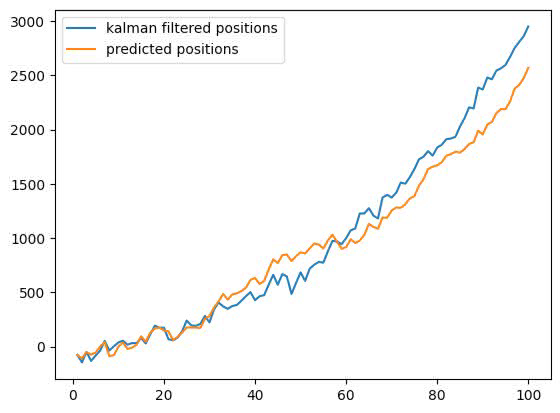
\includegraphics[width=216.05pt,height=159.35pt]{latexImage_fa4bb4e7fce925dd435a97b44febd006.png}}
\put(271.9,-361.611){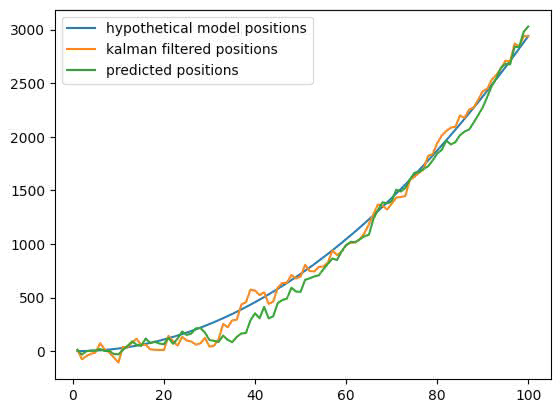
\includegraphics[width=226.25pt,height=166.9pt]{latexImage_8851090b138411bc19ab7bb3176e4db1.png}}
\put(55.85,-525.661){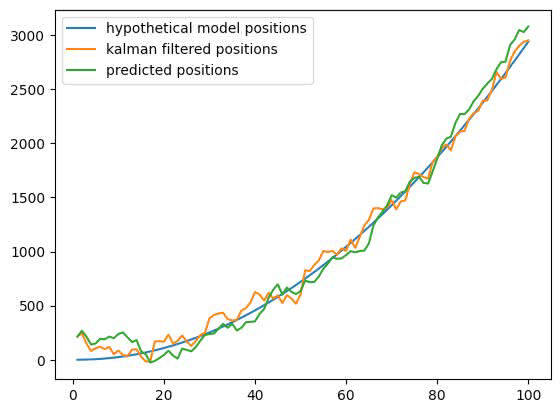
\includegraphics[width=217.55pt,height=160.45pt]{latexImage_5a74cbab4eab2fed6e8046fc580d5f28.png}}
\put(273.4,-525.661){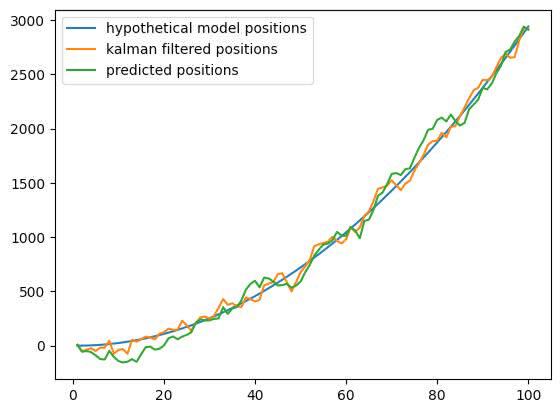
\includegraphics[width=222.45pt,height=164.05pt]{latexImage_8909ce613604599be0b156f8e5a04858.png}}
\put(56,-539.011){\fontsize{11}{1}\usefont{T1}{cmr}{m}{n}\selectfont\color{color_80434}图}
\put(69.2,-539.011){\fontsize{11}{1}\usefont{T1}{ptm}{m}{n}\selectfont\color{color_80434}1}
\put(74.304,-539.011){\fontsize{11}{1}\usefont{T1}{ptm}{m}{n}\selectfont\color{color_80434}1}
\put(79.705,-539.011){\fontsize{11}{1}\usefont{T1}{ptm}{m}{n}\selectfont\color{color_80434}.}
\put(56,-573.311){\fontsize{14}{1}\usefont{T1}{ptm}{b}{n}\selectfont\color{color_55609}c}
\put(62.2,-573.311){\fontsize{14}{1}\usefont{T1}{cmr}{m}{n}\selectfont\color{color_55609})模型分析}
\put(78,-621.711){\fontsize{16}{1}\usefont{T1}{ptm}{b}{n}\selectfont\color{color_55609}6}
\put(86,-621.711){\fontsize{16}{1}\usefont{T1}{cmr}{m}{n}\selectfont\color{color_55609}、}
\put(119,-621.711){\fontsize{16}{1}\usefont{T1}{cmr}{m}{n}\selectfont\color{color_55609}不确定性}
\end{picture}
\begin{tikzpicture}[overlay]
\path(0pt,0pt);
\filldraw[color_35327][even odd rule]
(116.7pt, -652.261pt) -- (128.65pt, -652.261pt)
 -- (128.65pt, -652.261pt)
 -- (128.65pt, -641.411pt)
 -- (128.65pt, -641.411pt)
 -- (116.7pt, -641.411pt) -- cycle
;
\end{tikzpicture}
\begin{picture}(-5,0)(2.5,0)
\put(116.8,-649.711){\fontsize{12}{1}\usefont{T1}{cmr}{m}{n}\selectfont\color{color_55609}}
\end{picture}
\begin{tikzpicture}[overlay]
\path(0pt,0pt);
\filldraw[color_35327][even odd rule]
(128.7pt, -652.261pt) -- (139.85pt, -652.261pt)
 -- (139.85pt, -652.261pt)
 -- (139.85pt, -641.411pt)
 -- (139.85pt, -641.411pt)
 -- (128.7pt, -641.411pt) -- cycle
;
\filldraw[color_283006][even odd rule]
(139.9pt, -652.261pt) -- (142.85pt, -652.261pt)
 -- (142.85pt, -652.261pt)
 -- (142.85pt, -638.511pt)
 -- (142.85pt, -638.511pt)
 -- (139.9pt, -638.511pt) -- cycle
;
\end{tikzpicture}
\begin{picture}(-5,0)(2.5,0)
\put(140,-649.711){\fontsize{12}{1}\usefont{T1}{ptm}{b}{n}\selectfont\color{color_55609} }
\end{picture}
\begin{tikzpicture}[overlay]
\path(0pt,0pt);
\filldraw[color_283006][even odd rule]
(142.9pt, -652.561pt) -- (502.85pt, -652.561pt)
 -- (502.85pt, -652.561pt)
 -- (502.85pt, -638.611pt)
 -- (502.85pt, -638.611pt)
 -- (142.9pt, -638.611pt) -- cycle
;
\end{tikzpicture}
\begin{picture}(-5,0)(2.5,0)
\put(143,-649.711){\fontsize{12}{1}\usefont{T1}{cmr}{m}{n}\selectfont\color{color_55609}在建立模型的过程中,}
\put(263,-649.711){\fontsize{12}{1}\usefont{T1}{cmr}{m}{n}\selectfont\color{color_55609}我}
\put(275,-649.711){\fontsize{12}{1}\usefont{T1}{cmr}{m}{n}\selectfont\color{color_55609}们}
\put(287,-649.711){\fontsize{12}{1}\usefont{T1}{cmr}{m}{n}\selectfont\color{color_55609}必须}
\put(311,-649.711){\fontsize{12}{1}\usefont{T1}{cmr}{m}{n}\selectfont\color{color_55609}要}
\put(323,-649.711){\fontsize{12}{1}\usefont{T1}{cmr}{m}{n}\selectfont\color{color_55609}考虑很}
\put(359,-649.711){\fontsize{12}{1}\usefont{T1}{cmr}{m}{n}\selectfont\color{color_55609}多不确定因素,比如地}
\put(479,-649.711){\fontsize{12}{1}\usefont{T1}{cmr}{m}{n}\selectfont\color{color_55609}质}
\put(491,-649.711){\fontsize{12}{1}\usefont{T1}{cmr}{m}{n}\selectfont\color{color_55609}环}
\end{picture}
\begin{tikzpicture}[overlay]
\path(0pt,0pt);
\filldraw[color_283006][even odd rule]
(116.7pt, -676.361pt) -- (404.65pt, -676.361pt)
 -- (404.65pt, -676.361pt)
 -- (404.65pt, -662.411pt)
 -- (404.65pt, -662.411pt)
 -- (116.7pt, -662.411pt) -- cycle
;
\end{tikzpicture}
\begin{picture}(-5,0)(2.5,0)
\put(116.8,-673.611){\fontsize{12}{1}\usefont{T1}{cmr}{m}{n}\selectfont\color{color_55609}境,}
\put(140.8,-673.611){\fontsize{12}{1}\usefont{T1}{cmr}{m}{n}\selectfont\color{color_55609}自身姿}
\put(176.8,-673.611){\fontsize{12}{1}\usefont{T1}{cmr}{m}{n}\selectfont\color{color_55609}态等等,}
\put(224.8,-673.611){\fontsize{12}{1}\usefont{T1}{cmr}{m}{n}\selectfont\color{color_55609}我}
\put(236.8,-673.611){\fontsize{12}{1}\usefont{T1}{cmr}{m}{n}\selectfont\color{color_55609}们}
\put(248.8,-673.611){\fontsize{12}{1}\usefont{T1}{cmr}{m}{n}\selectfont\color{color_55609}尽}
\put(260.8,-673.611){\fontsize{12}{1}\usefont{T1}{cmr}{m}{n}\selectfont\color{color_55609}可能地}
\put(296.8,-673.611){\fontsize{12}{1}\usefont{T1}{cmr}{m}{n}\selectfont\color{color_55609}列}
\put(308.8,-673.611){\fontsize{12}{1}\usefont{T1}{cmr}{m}{n}\selectfont\color{color_55609}出这些不确定因素}
\end{picture}
\begin{tikzpicture}[overlay]
\path(0pt,0pt);
\filldraw[color_283006][even odd rule]
(404.7pt, -676.161pt) -- (407.65pt, -676.161pt)
 -- (407.65pt, -676.161pt)
 -- (407.65pt, -662.411pt)
 -- (407.65pt, -662.411pt)
 -- (404.7pt, -662.411pt) -- cycle
;
\end{tikzpicture}
\begin{picture}(-5,0)(2.5,0)
\put(404.8,-673.611){\fontsize{12}{1}\usefont{T1}{ptm}{b}{n}\selectfont\color{color_55609}.  }
\end{picture}
\begin{tikzpicture}[overlay]
\path(0pt,0pt);
\filldraw[color_35327][even odd rule]
(55.9pt, -725.561pt) -- (67.85pt, -725.561pt)
 -- (67.85pt, -725.561pt)
 -- (67.85pt, -714.711pt)
 -- (67.85pt, -714.711pt)
 -- (55.9pt, -714.711pt) -- cycle
;
\end{tikzpicture}
\begin{picture}(-5,0)(2.5,0)
\put(56,-723.011){\fontsize{12}{1}\usefont{T1}{cmr}{m}{n}\selectfont\color{color_80434}}
\end{picture}
\begin{tikzpicture}[overlay]
\path(0pt,0pt);
\filldraw[color_35327][even odd rule]
(67.9pt, -725.561pt) -- (72.65pt, -725.561pt)
 -- (72.65pt, -725.561pt)
 -- (72.65pt, -714.711pt)
 -- (72.65pt, -714.711pt)
 -- (67.9pt, -714.711pt) -- cycle
;
\filldraw[color_283006][even odd rule]
(72.7pt, -725.861pt) -- (504.65pt, -725.861pt)
 -- (504.65pt, -725.861pt)
 -- (504.65pt, -711.911pt)
 -- (504.65pt, -711.911pt)
 -- (72.7pt, -711.911pt) -- cycle
;
\end{tikzpicture}
\begin{picture}(-5,0)(2.5,0)
\put(72.8,-723.011){\fontsize{12}{1}\usefont{T1}{cmr}{m}{n}\selectfont\color{color_80434}探险过程中,}
\put(144.8,-723.011){\fontsize{12}{1}\usefont{T1}{cmr}{m}{n}\selectfont\color{color_80434}由}
\put(156.8,-723.011){\fontsize{12}{1}\usefont{T1}{cmr}{m}{n}\selectfont\color{color_80434}于海底地}
\put(204.8,-723.011){\fontsize{12}{1}\usefont{T1}{cmr}{m}{n}\selectfont\color{color_80434}形具}
\put(228.8,-723.011){\fontsize{12}{1}\usefont{T1}{cmr}{m}{n}\selectfont\color{color_80434}有}
\put(240.8,-723.011){\fontsize{12}{1}\usefont{T1}{cmr}{m}{n}\selectfont\color{color_80434}特殊}
\put(264.8,-723.011){\fontsize{12}{1}\usefont{T1}{cmr}{m}{n}\selectfont\color{color_80434}的}
\put(276.8,-723.011){\fontsize{12}{1}\usefont{T1}{cmr}{m}{n}\selectfont\color{color_80434}构}
\put(288.8,-723.011){\fontsize{12}{1}\usefont{T1}{cmr}{m}{n}\selectfont\color{color_80434}成和地}
\put(324.8,-723.011){\fontsize{12}{1}\usefont{T1}{cmr}{m}{n}\selectfont\color{color_80434}貌}
\put(336.8,-723.011){\fontsize{12}{1}\usefont{T1}{cmr}{m}{n}\selectfont\color{color_80434}特}
\put(348.8,-723.011){\fontsize{12}{1}\usefont{T1}{cmr}{m}{n}\selectfont\color{color_80434}征}
\put(360.8,-723.011){\fontsize{12}{1}\usefont{T1}{cmr}{m}{n}\selectfont\color{color_80434},使得}
\put(396.8,-723.011){\fontsize{12}{1}\usefont{T1}{cmr}{m}{n}\selectfont\color{color_80434}某}
\put(408.8,-723.011){\fontsize{12}{1}\usefont{T1}{cmr}{m}{n}\selectfont\color{color_80434}些区域水流}
\put(468.8,-723.011){\fontsize{12}{1}\usefont{T1}{cmr}{m}{n}\selectfont\color{color_80434}速度}
\put(492.8,-723.011){\fontsize{12}{1}\usefont{T1}{cmr}{m}{n}\selectfont\color{color_80434}较}
\end{picture}
\begin{tikzpicture}[overlay]
\path(0pt,0pt);
\filldraw[color_283006][even odd rule]
(72.7pt, -746.361pt) -- (228.65pt, -746.361pt)
 -- (228.65pt, -746.361pt)
 -- (228.65pt, -732.411pt)
 -- (228.65pt, -732.411pt)
 -- (72.7pt, -732.411pt) -- cycle
;
\end{tikzpicture}
\begin{picture}(-5,0)(2.5,0)
\put(72.8,-743.511){\fontsize{12}{1}\usefont{T1}{cmr}{m}{n}\selectfont\color{color_80434}快}
\put(84.8,-743.511){\fontsize{12}{1}\usefont{T1}{cmr}{m}{n}\selectfont\color{color_80434},对潜水器的}
\put(156.8,-743.511){\fontsize{12}{1}\usefont{T1}{cmr}{m}{n}\selectfont\color{color_80434}运}
\put(168.8,-743.511){\fontsize{12}{1}\usefont{T1}{cmr}{m}{n}\selectfont\color{color_80434}动}
\put(180.8,-743.511){\fontsize{12}{1}\usefont{T1}{cmr}{m}{n}\selectfont\color{color_80434}产生影响}
\end{picture}
\begin{tikzpicture}[overlay]
\path(0pt,0pt);
\filldraw[color_283006][even odd rule]
(228.7pt, -746.061pt) -- (231.65pt, -746.061pt)
 -- (231.65pt, -746.061pt)
 -- (231.65pt, -732.311pt)
 -- (231.65pt, -732.311pt)
 -- (228.7pt, -732.311pt) -- cycle
;
\end{tikzpicture}
\begin{picture}(-5,0)(2.5,0)
\put(228.8,-743.511){\fontsize{12}{1}\usefont{T1}{ptm}{m}{n}\selectfont\color{color_80434}.}
\end{picture}
\begin{tikzpicture}[overlay]
\path(0pt,0pt);
\filldraw[color_283006][even odd rule]
(231.7pt, -746.361pt) -- (507.65pt, -746.361pt)
 -- (507.65pt, -746.361pt)
 -- (507.65pt, -732.411pt)
 -- (507.65pt, -732.411pt)
 -- (231.7pt, -732.411pt) -- cycle
;
\end{tikzpicture}
\begin{picture}(-5,0)(2.5,0)
\put(231.8,-743.511){\fontsize{12}{1}\usefont{T1}{cmr}{m}{n}\selectfont\color{color_80434}此外,在潜水器}
\put(315.8,-743.511){\fontsize{12}{1}\usefont{T1}{cmr}{m}{n}\selectfont\color{color_80434}运}
\put(327.8,-743.511){\fontsize{12}{1}\usefont{T1}{cmr}{m}{n}\selectfont\color{color_80434}动的过程中,}
\put(399.8,-743.511){\fontsize{12}{1}\usefont{T1}{cmr}{m}{n}\selectfont\color{color_80434}若遇}
\put(423.8,-743.511){\fontsize{12}{1}\usefont{T1}{cmr}{m}{n}\selectfont\color{color_80434}到了}
\put(447.8,-743.511){\fontsize{12}{1}\usefont{T1}{cmr}{m}{n}\selectfont\color{color_80434}强劲}
\put(471.8,-743.511){\fontsize{12}{1}\usefont{T1}{cmr}{m}{n}\selectfont\color{color_80434}的洋流}
\end{picture}
\begin{tikzpicture}[overlay]
\path(0pt,0pt);
\filldraw[color_283006][even odd rule]
(507.7pt, -746.361pt) -- (519.65pt, -746.361pt)
 -- (519.65pt, -746.361pt)
 -- (519.65pt, -732.411pt)
 -- (519.65pt, -732.411pt)
 -- (507.7pt, -732.411pt) -- cycle
;
\end{tikzpicture}
\begin{picture}(-5,0)(2.5,0)
\put(507.8,-743.511){\fontsize{12}{1}\usefont{T1}{cmr}{m}{n}\selectfont\color{color_80434},}
\end{picture}
\newpage
\begin{tikzpicture}[overlay]
\path(0pt,0pt);
\filldraw[color_283006][even odd rule]
(72.7pt, -78.76099pt) -- (300.65pt, -78.76099pt)
 -- (300.65pt, -78.76099pt)
 -- (300.65pt, -64.81097pt)
 -- (300.65pt, -64.81097pt)
 -- (72.7pt, -64.81097pt) -- cycle
;
\end{tikzpicture}
\begin{picture}(-5,0)(2.5,0)
\put(72.8,-76.01099){\fontsize{12}{1}\usefont{T1}{cmr}{m}{n}\selectfont\color{color_80434}可能}
\put(96.8,-76.01099){\fontsize{12}{1}\usefont{T1}{cmr}{m}{n}\selectfont\color{color_80434}会}
\put(108.8,-76.01099){\fontsize{12}{1}\usefont{T1}{cmr}{m}{n}\selectfont\color{color_80434}对潜水器的}
\put(168.8,-76.01099){\fontsize{12}{1}\usefont{T1}{cmr}{m}{n}\selectfont\color{color_80434}运}
\put(180.8,-76.01099){\fontsize{12}{1}\usefont{T1}{cmr}{m}{n}\selectfont\color{color_80434}动方向和}
\put(228.8,-76.01099){\fontsize{12}{1}\usefont{T1}{cmr}{m}{n}\selectfont\color{color_80434}速度造}
\put(264.8,-76.01099){\fontsize{12}{1}\usefont{T1}{cmr}{m}{n}\selectfont\color{color_80434}成}
\put(276.8,-76.01099){\fontsize{12}{1}\usefont{T1}{cmr}{m}{n}\selectfont\color{color_80434}影响}
\end{picture}
\begin{tikzpicture}[overlay]
\path(0pt,0pt);
\filldraw[color_283006][even odd rule]
(300.7pt, -78.56097pt) -- (303.65pt, -78.56097pt)
 -- (303.65pt, -78.56097pt)
 -- (303.65pt, -64.81097pt)
 -- (303.65pt, -64.81097pt)
 -- (300.7pt, -64.81097pt) -- cycle
;
\end{tikzpicture}
\begin{picture}(-5,0)(2.5,0)
\put(300.8,-76.01099){\fontsize{12}{1}\usefont{T1}{ptm}{m}{n}\selectfont\color{color_80434}.}
\put(56,-115.711){\fontsize{12}{1}\usefont{T1}{cmr}{m}{n}\selectfont\color{color_80434}}
\put(72.8,-115.711){\fontsize{12}{1}\usefont{T1}{cmr}{m}{n}\selectfont\color{color_80434}首先}
\put(96.8,-115.711){\fontsize{12}{1}\usefont{T1}{cmr}{m}{n}\selectfont\color{color_80434}从}
\put(111.2,-115.711){\fontsize{12}{1}\usefont{T1}{ptm}{m}{n}\selectfont\color{color_80434}G}
\put(119.888,-115.711){\fontsize{12}{1}\usefont{T1}{ptm}{m}{n}\selectfont\color{color_80434}E}
\put(127.184,-115.711){\fontsize{12}{1}\usefont{T1}{ptm}{m}{n}\selectfont\color{color_80434}BC}
\put(143.072,-115.711){\fontsize{12}{1}\usefont{T1}{ptm}{m}{n}\selectfont\color{color_80434}O}
\put(154.2,-115.711){\fontsize{12}{1}\usefont{T1}{cmr}{m}{n}\selectfont\color{color_80434}网}
\put(166.2,-115.711){\fontsize{12}{1}\usefont{T1}{cmr}{m}{n}\selectfont\color{color_80434}站获}
\put(190.2,-115.711){\fontsize{12}{1}\usefont{T1}{cmr}{m}{n}\selectfont\color{color_80434}取}
\put(202.2,-115.711){\fontsize{12}{1}\usefont{T1}{cmr}{m}{n}\selectfont\color{color_80434}海底地}
\put(238.2,-115.711){\fontsize{12}{1}\usefont{T1}{cmr}{m}{n}\selectfont\color{color_80434}形}
\put(250.2,-115.711){\fontsize{12}{1}\usefont{T1}{cmr}{m}{n}\selectfont\color{color_80434}数据,使用}
\put(312.6,-115.711){\fontsize{12}{1}\usefont{T1}{ptm}{m}{n}\selectfont\color{color_80434}G}
\put(321.288,-115.711){\fontsize{12}{1}\usefont{T1}{ptm}{m}{n}\selectfont\color{color_80434}l}
\put(324.588,-115.711){\fontsize{12}{1}\usefont{T1}{ptm}{m}{n}\selectfont\color{color_80434}oba}
\put(341.892,-115.711){\fontsize{12}{1}\usefont{T1}{ptm}{m}{n}\selectfont\color{color_80434}l}
\put(345.276,-115.711){\fontsize{12}{1}\usefont{T1}{ptm}{m}{n}\selectfont\color{color_80434} M}
\put(358.968,-115.711){\fontsize{12}{1}\usefont{T1}{ptm}{m}{n}\selectfont\color{color_80434}a}
\put(364.2719,-115.711){\fontsize{12}{1}\usefont{T1}{ptm}{m}{n}\selectfont\color{color_80434}ppe}
\put(381.5759,-115.711){\fontsize{12}{1}\usefont{T1}{ptm}{m}{n}\selectfont\color{color_80434}r pro v23.1}
\put(437,-115.711){\fontsize{12}{1}\usefont{T1}{cmr}{m}{n}\selectfont\color{color_80434}分析海底地}
\put(497,-115.711){\fontsize{12}{1}\usefont{T1}{cmr}{m}{n}\selectfont\color{color_80434}形}
\put(72.8,-129.711){\fontsize{12}{1}\usefont{T1}{cmr}{m}{n}\selectfont\color{color_80434}局}
\put(84.8,-129.711){\fontsize{12}{1}\usefont{T1}{cmr}{m}{n}\selectfont\color{color_80434}部}
\put(96.8,-129.711){\fontsize{12}{1}\usefont{T1}{cmr}{m}{n}\selectfont\color{color_80434}特}
\put(108.8,-129.711){\fontsize{12}{1}\usefont{T1}{cmr}{m}{n}\selectfont\color{color_80434}征}
\put(120.8,-129.711){\fontsize{12}{1}\usefont{T1}{cmr}{m}{n}\selectfont\color{color_80434}以及部分参数,}
\put(204.8,-129.711){\fontsize{12}{1}\usefont{T1}{cmr}{m}{n}\selectfont\color{color_80434}再}
\put(216.8,-129.711){\fontsize{12}{1}\usefont{T1}{cmr}{m}{n}\selectfont\color{color_80434}使用}
\put(243.2,-129.711){\fontsize{12}{1}\usefont{T1}{ptm}{m}{n}\selectfont\color{color_80434}pyt}
\put(258.5,-129.711){\fontsize{12}{1}\usefont{T1}{ptm}{m}{n}\selectfont\color{color_80434}hon}
\put(278.9,-129.711){\fontsize{12}{1}\usefont{T1}{cmr}{m}{n}\selectfont\color{color_80434}对数据进行可}
\put(350.9,-129.711){\fontsize{12}{1}\usefont{T1}{cmr}{m}{n}\selectfont\color{color_80434}视}
\put(362.9,-129.711){\fontsize{12}{1}\usefont{T1}{cmr}{m}{n}\selectfont\color{color_80434}化}
\put(374.9,-129.711){\fontsize{12}{1}\usefont{T1}{cmr}{m}{n}\selectfont\color{color_80434}处}
\put(386.9,-129.711){\fontsize{12}{1}\usefont{T1}{cmr}{m}{n}\selectfont\color{color_80434}理}
\put(398.9,-129.711){\fontsize{12}{1}\usefont{T1}{ptm}{m}{n}\selectfont\color{color_80434}.}
\put(116.65,-375.961){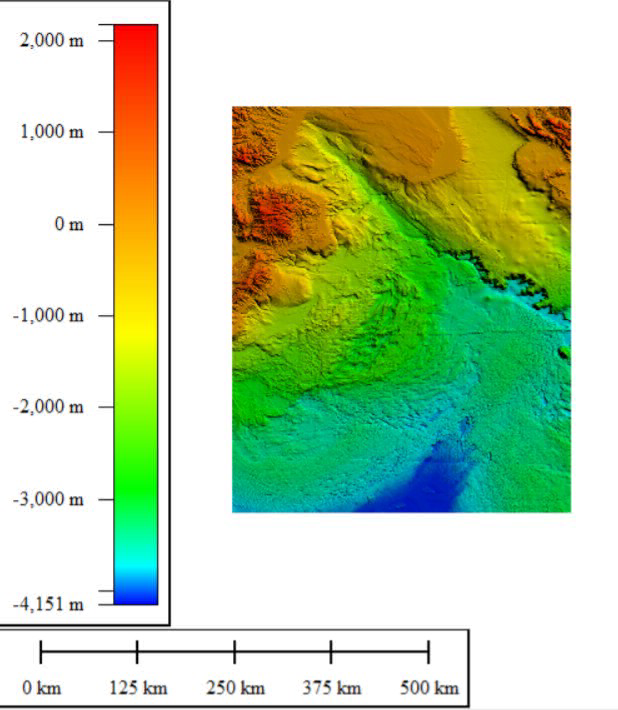
\includegraphics[width=188.8pt,height=216.95pt]{latexImage_5075d423f352345a98545c5b5a81e6aa.png}}
\put(305.45,-375.961){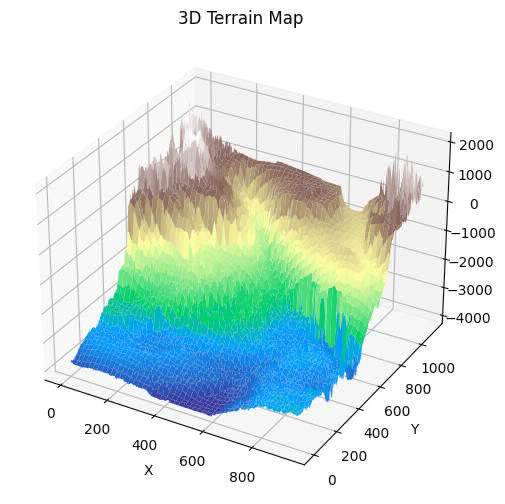
\includegraphics[width=197.9pt,height=197.5pt]{latexImage_c207a0513ae6cb35ebac7e978be8b6b5.png}}
\put(116.8,-401.611){\fontsize{11}{1}\usefont{T1}{ptm}{m}{n}\selectfont\color{color_80434} }
\put(119.495,-401.611){\fontsize{11}{1}\usefont{T1}{ptm}{m}{n}\selectfont\color{color_80434} }
\put(122.289,-401.611){\fontsize{11}{1}\usefont{T1}{ptm}{m}{n}\selectfont\color{color_80434} }
\put(124.984,-401.611){\fontsize{11}{1}\usefont{T1}{ptm}{m}{n}\selectfont\color{color_80434} }
\put(127.778,-401.611){\fontsize{11}{1}\usefont{T1}{ptm}{m}{n}\selectfont\color{color_80434} }
\put(130.473,-401.611){\fontsize{11}{1}\usefont{T1}{ptm}{m}{n}\selectfont\color{color_80434} }
\put(133.267,-401.611){\fontsize{11}{1}\usefont{T1}{ptm}{m}{n}\selectfont\color{color_80434} }
\put(135.9621,-401.611){\fontsize{11}{1}\usefont{T1}{ptm}{m}{n}\selectfont\color{color_80434} }
\put(138.7561,-401.611){\fontsize{11}{1}\usefont{T1}{ptm}{m}{n}\selectfont\color{color_80434} }
\put(141.4511,-401.611){\fontsize{11}{1}\usefont{T1}{ptm}{m}{n}\selectfont\color{color_80434} }
\put(144.2451,-401.611){\fontsize{11}{1}\usefont{T1}{ptm}{m}{n}\selectfont\color{color_80434} }
\put(146.9401,-401.611){\fontsize{11}{1}\usefont{T1}{ptm}{m}{n}\selectfont\color{color_80434} }
\put(149.8,-401.611){\fontsize{11}{1}\usefont{T1}{cmr}{m}{n}\selectfont\color{color_80434}图}
\put(163,-401.611){\fontsize{11}{1}\usefont{T1}{ptm}{m}{n}\selectfont\color{color_80434}12}
\put(173.901,-401.611){\fontsize{11}{1}\usefont{T1}{ptm}{m}{n}\selectfont\color{color_80434}.}
\put(264.7,-401.611){\fontsize{11}{1}\usefont{T1}{cmr}{m}{n}\selectfont\color{color_80434}                            }
\put(176.7,-401.611){\fontsize{11}{1}\usefont{T1}{cmr}{m}{n}\selectfont\color{color_80434}爱奥尼亚海地地}
\put(253.7,-401.611){\fontsize{11}{1}\usefont{T1}{cmr}{m}{n}\selectfont\color{color_80434}形}
\put(362.688,-401.611){\fontsize{11}{1}\usefont{T1}{cmr}{m}{n}\selectfont\color{color_80434}图}
\put(375.9,-401.611){\fontsize{11}{1}\usefont{T1}{ptm}{m}{n}\selectfont\color{color_80434}13.}
\put(466.7,-401.611){\fontsize{11}{1}\usefont{T1}{cmr}{m}{n}\selectfont\color{color_80434}            }
\put(389.7,-401.611){\fontsize{11}{1}\usefont{T1}{cmr}{m}{n}\selectfont\color{color_80434}爱奥尼亚海洋流}
\put(56,-421.311){\fontsize{11}{1}\usefont{T1}{ptm}{m}{n}\selectfont\color{color_29791} }
\put(116.8,-437.911){\fontsize{12}{1}\usefont{T1}{cmr}{m}{n}\selectfont\color{color_55609}}
\put(140,-437.911){\fontsize{12}{1}\usefont{T1}{cmr}{m}{n}\selectfont\color{color_55609}分析:爱奥尼亚海}
\put(236,-437.911){\fontsize{12}{1}\usefont{T1}{cmr}{m}{n}\selectfont\color{color_55609}是}
\put(248,-437.911){\fontsize{12}{1}\usefont{T1}{cmr}{m}{n}\selectfont\color{color_55609}地中海最}
\put(296,-437.911){\fontsize{12}{1}\usefont{T1}{cmr}{m}{n}\selectfont\color{color_55609}深}
\put(308,-437.911){\fontsize{12}{1}\usefont{T1}{cmr}{m}{n}\selectfont\color{color_55609}的}
\put(320,-437.911){\fontsize{12}{1}\usefont{T1}{cmr}{m}{n}\selectfont\color{color_55609}子盆}
\put(344,-437.911){\fontsize{12}{1}\usefont{T1}{cmr}{m}{n}\selectfont\color{color_55609}地,}
\put(368,-437.911){\fontsize{12}{1}\usefont{T1}{cmr}{m}{n}\selectfont\color{color_55609}由几}
\put(392,-437.911){\fontsize{12}{1}\usefont{T1}{cmr}{m}{n}\selectfont\color{color_55609}个}
\put(404,-437.911){\fontsize{12}{1}\usefont{T1}{cmr}{m}{n}\selectfont\color{color_55609}深度超}
\put(440,-437.911){\fontsize{12}{1}\usefont{T1}{cmr}{m}{n}\selectfont\color{color_55609}过}
\put(454.4,-437.911){\fontsize{12}{1}\usefont{T1}{ptm}{b}{n}\selectfont\color{color_55609}4000}
\put(478.4,-437.911){\fontsize{12}{1}\usefont{T1}{ptm}{b}{n}\selectfont\color{color_55609} }
\put(481.4,-437.911){\fontsize{12}{1}\usefont{T1}{ptm}{b}{n}\selectfont\color{color_55609}m}
\put(493.8,-437.911){\fontsize{12}{1}\usefont{T1}{cmr}{m}{n}\selectfont\color{color_55609}的}
\put(116.8,-461.811){\fontsize{12}{1}\usefont{T1}{cmr}{m}{n}\selectfont\color{color_55609}海}
\put(128.8,-461.811){\fontsize{12}{1}\usefont{T1}{cmr}{m}{n}\selectfont\color{color_55609}沟}
\put(140.8,-461.811){\fontsize{12}{1}\usefont{T1}{cmr}{m}{n}\selectfont\color{color_55609}和高}
\put(164.8,-461.811){\fontsize{12}{1}\usefont{T1}{cmr}{m}{n}\selectfont\color{color_55609}原}
\put(176.8,-461.811){\fontsize{12}{1}\usefont{T1}{cmr}{m}{n}\selectfont\color{color_55609}组}
\put(188.8,-461.811){\fontsize{12}{1}\usefont{T1}{cmr}{m}{n}\selectfont\color{color_55609}成}
\put(200.8,-461.811){\fontsize{12}{1}\usefont{T1}{ptm}{b}{n}\selectfont\color{color_55609}.}
\put(203.8,-461.811){\fontsize{12}{1}\usefont{T1}{cmr}{m}{n}\selectfont\color{color_55609}由}
\put(218.2,-461.811){\fontsize{12}{1}\usefont{T1}{ptm}{b}{n}\selectfont\color{color_55609}3}
\put(224.104,-461.811){\fontsize{12}{1}\usefont{T1}{ptm}{b}{n}\selectfont\color{color_55609}D}
\put(232.792,-461.811){\fontsize{12}{1}\usefont{T1}{ptm}{b}{n}\selectfont\color{color_55609} }
\put(235.588,-461.811){\fontsize{12}{1}\usefont{T1}{ptm}{b}{n}\selectfont\color{color_55609}T}
\put(242.392,-461.811){\fontsize{12}{1}\usefont{T1}{ptm}{b}{n}\selectfont\color{color_55609}e}
\put(247.78,-461.811){\fontsize{12}{1}\usefont{T1}{ptm}{b}{n}\selectfont\color{color_55609}r}
\put(253.168,-461.811){\fontsize{12}{1}\usefont{T1}{ptm}{b}{n}\selectfont\color{color_55609}r}
\put(258.472,-461.811){\fontsize{12}{1}\usefont{T1}{ptm}{b}{n}\selectfont\color{color_55609}i}
\put(261.772,-461.811){\fontsize{12}{1}\usefont{T1}{ptm}{b}{n}\selectfont\color{color_55609}an}
\put(274.456,-461.811){\fontsize{12}{1}\usefont{T1}{ptm}{b}{n}\selectfont\color{color_55609} M}
\put(288.7599,-461.811){\fontsize{12}{1}\usefont{T1}{ptm}{b}{n}\selectfont\color{color_55609}ap}
\put(303.9,-461.811){\fontsize{12}{1}\usefont{T1}{cmr}{m}{n}\selectfont\color{color_55609}可以}
\put(327.9,-461.811){\fontsize{12}{1}\usefont{T1}{cmr}{m}{n}\selectfont\color{color_55609}看}
\put(339.9,-461.811){\fontsize{12}{1}\usefont{T1}{cmr}{m}{n}\selectfont\color{color_55609}出爱奥尼亚海海底}
\put(435.9,-461.811){\fontsize{12}{1}\usefont{T1}{cmr}{m}{n}\selectfont\color{color_55609}跨}
\put(447.9,-461.811){\fontsize{12}{1}\usefont{T1}{cmr}{m}{n}\selectfont\color{color_55609}度}
\put(459.9,-461.811){\fontsize{12}{1}\usefont{T1}{cmr}{m}{n}\selectfont\color{color_55609}在}
\put(474.3,-461.811){\fontsize{12}{1}\usefont{T1}{ptm}{b}{n}\selectfont\color{color_55609}1000-}
\put(116.8,-485.611){\fontsize{12}{1}\usefont{T1}{ptm}{b}{n}\selectfont\color{color_55609}2000}
\put(143.2,-485.611){\fontsize{12}{1}\usefont{T1}{cmr}{m}{n}\selectfont\color{color_55609}以}
\put(155.2,-485.611){\fontsize{12}{1}\usefont{T1}{cmr}{m}{n}\selectfont\color{color_55609}内}
\put(167.2,-485.611){\fontsize{12}{1}\usefont{T1}{cmr}{m}{n}\selectfont\color{color_55609},探险}
\put(203.2,-485.611){\fontsize{12}{1}\usefont{T1}{cmr}{m}{n}\selectfont\color{color_55609}人员}
\put(227.2,-485.611){\fontsize{12}{1}\usefont{T1}{cmr}{m}{n}\selectfont\color{color_55609}需要}
\put(251.2,-485.611){\fontsize{12}{1}\usefont{T1}{cmr}{m}{n}\selectfont\color{color_55609}注}
\put(263.2,-485.611){\fontsize{12}{1}\usefont{T1}{cmr}{m}{n}\selectfont\color{color_55609}意}
\put(275.2,-485.611){\fontsize{12}{1}\usefont{T1}{cmr}{m}{n}\selectfont\color{color_55609}自己}
\put(299.2,-485.611){\fontsize{12}{1}\usefont{T1}{cmr}{m}{n}\selectfont\color{color_55609}的}
\put(311.2,-485.611){\fontsize{12}{1}\usefont{T1}{cmr}{m}{n}\selectfont\color{color_55609}人}
\put(323.2,-485.611){\fontsize{12}{1}\usefont{T1}{cmr}{m}{n}\selectfont\color{color_55609}身}
\put(335.2,-485.611){\fontsize{12}{1}\usefont{T1}{cmr}{m}{n}\selectfont\color{color_55609}安全,以防失去与主船的通信}
\put(491.2,-485.611){\fontsize{12}{1}\usefont{T1}{ptm}{b}{n}\selectfont\color{color_55609}.}
\put(56,-533.611){\fontsize{18}{1}\usefont{T1}{cmr}{m}{n}\selectfont\color{color_55609}五}
\put(74,-533.611){\fontsize{18}{1}\usefont{T1}{cmr}{m}{n}\selectfont\color{color_55609}、}
\put(98,-533.611){\fontsize{18}{1}\usefont{T1}{cmr}{m}{n}\selectfont\color{color_55609}设备}
\put(134,-533.611){\fontsize{18}{1}\usefont{T1}{cmr}{m}{n}\selectfont\color{color_55609}选择}
\put(78,-567.511){\fontsize{16}{1}\usefont{T1}{ptm}{b}{n}\selectfont\color{color_55609}1}
\put(86,-567.511){\fontsize{16}{1}\usefont{T1}{cmr}{m}{n}\selectfont\color{color_55609}、}
\put(119,-567.511){\fontsize{16}{1}\usefont{T1}{cmr}{m}{n}\selectfont\color{color_55609}问题分析}
\put(56,-598.511){\fontsize{12}{1}\usefont{T1}{cmr}{m}{n}\selectfont\color{color_80434}在这个问题上,}
\put(140,-598.511){\fontsize{12}{1}\usefont{T1}{cmr}{m}{n}\selectfont\color{color_80434}我}
\put(152,-598.511){\fontsize{12}{1}\usefont{T1}{cmr}{m}{n}\selectfont\color{color_80434}们需要建立一个}
\put(236,-598.511){\fontsize{12}{1}\usefont{T1}{cmr}{m}{n}\selectfont\color{color_80434}综}
\put(248,-598.511){\fontsize{12}{1}\usefont{T1}{cmr}{m}{n}\selectfont\color{color_80434}合效益分析模型}
\put(332,-598.511){\fontsize{12}{1}\usefont{T1}{cmr}{m}{n}\selectfont\color{color_80434}来}
\put(344,-598.511){\fontsize{12}{1}\usefont{T1}{cmr}{m}{n}\selectfont\color{color_80434}确定}
\put(368,-598.511){\fontsize{12}{1}\usefont{T1}{cmr}{m}{n}\selectfont\color{color_80434}哪}
\put(380,-598.511){\fontsize{12}{1}\usefont{T1}{cmr}{m}{n}\selectfont\color{color_80434}些设备}
\put(416,-598.511){\fontsize{12}{1}\usefont{T1}{cmr}{m}{n}\selectfont\color{color_80434}是}
\put(428,-598.511){\fontsize{12}{1}\usefont{T1}{cmr}{m}{n}\selectfont\color{color_80434}最}
\put(440,-598.511){\fontsize{12}{1}\usefont{T1}{cmr}{m}{n}\selectfont\color{color_80434}好}
\put(452,-598.511){\fontsize{12}{1}\usefont{T1}{cmr}{m}{n}\selectfont\color{color_80434}的,}
\put(476,-598.511){\fontsize{12}{1}\usefont{T1}{cmr}{m}{n}\selectfont\color{color_80434}我}
\put(488,-598.511){\fontsize{12}{1}\usefont{T1}{cmr}{m}{n}\selectfont\color{color_80434}们}
\put(56,-612.611){\fontsize{12}{1}\usefont{T1}{cmr}{m}{n}\selectfont\color{color_80434}需要分析}
\put(104,-612.611){\fontsize{12}{1}\usefont{T1}{cmr}{m}{n}\selectfont\color{color_80434}哪}
\put(116,-612.611){\fontsize{12}{1}\usefont{T1}{cmr}{m}{n}\selectfont\color{color_80434}些设备}
\put(152,-612.611){\fontsize{12}{1}\usefont{T1}{cmr}{m}{n}\selectfont\color{color_80434}综}
\put(164,-612.611){\fontsize{12}{1}\usefont{T1}{cmr}{m}{n}\selectfont\color{color_80434}合成本最}
\put(212,-612.611){\fontsize{12}{1}\usefont{T1}{cmr}{m}{n}\selectfont\color{color_80434}低}
\put(224,-612.611){\fontsize{12}{1}\usefont{T1}{cmr}{m}{n}\selectfont\color{color_80434},效果最}
\put(272,-612.611){\fontsize{12}{1}\usefont{T1}{cmr}{m}{n}\selectfont\color{color_80434}好}
\put(284,-612.611){\fontsize{12}{1}\usefont{T1}{ptm}{m}{n}\selectfont\color{color_80434}.}
\put(78,-633.411){\fontsize{16}{1}\usefont{T1}{ptm}{b}{n}\selectfont\color{color_55609}2}
\put(86,-633.411){\fontsize{16}{1}\usefont{T1}{cmr}{m}{n}\selectfont\color{color_55609}、}
\put(119,-633.411){\fontsize{16}{1}\usefont{T1}{cmr}{m}{n}\selectfont\color{color_55609}模型的准备}
\put(100,-663.411){\fontsize{14}{1}\usefont{T1}{ptm}{b}{n}\selectfont\color{color_55609}a}
\put(106.902,-663.411){\fontsize{14}{1}\usefont{T1}{ptm}{b}{n}\selectfont\color{color_55609})}
\put(116.8,-663.411){\fontsize{14}{1}\usefont{T1}{cmr}{m}{n}\selectfont\color{color_55609}搜索设备}
\put(56,-691.311){\fontsize{11}{1}\usefont{T1}{cmr}{m}{n}\selectfont\color{color_80434}我}
\put(67,-691.311){\fontsize{11}{1}\usefont{T1}{cmr}{m}{n}\selectfont\color{color_80434}们准备了以下比较常用的搜寻设备}
\put(56,-707.111){\fontsize{11}{1}\usefont{T1}{cmr}{m}{n}\selectfont\color{color_80434}}
\end{picture}
\begin{tikzpicture}[overlay]
\path(0pt,0pt);
\filldraw[color_283006][even odd rule]
(72.7pt, -709.561pt) -- (131.75pt, -709.561pt)
 -- (131.75pt, -709.561pt)
 -- (131.75pt, -697.411pt)
 -- (131.75pt, -697.411pt)
 -- (72.7pt, -697.411pt) -- cycle
;
\end{tikzpicture}
\begin{picture}(-5,0)(2.5,0)
\put(72.8,-707.111){\fontsize{10.5}{1}\usefont{T1}{ptm}{b}{n}\selectfont\color{color_80434}K}
\put(80.8955,-707.111){\fontsize{10.5}{1}\usefont{T1}{ptm}{b}{n}\selectfont\color{color_80434}le}
\put(91.5845,-707.111){\fontsize{10.5}{1}\usefont{T1}{ptm}{b}{n}\selectfont\color{color_80434}in}
\put(102.662,-707.111){\fontsize{10.5}{1}\usefont{T1}{ptm}{b}{n}\selectfont\color{color_80434}3000}
\end{picture}
\begin{tikzpicture}[overlay]
\path(0pt,0pt);
\filldraw[color_283006][even odd rule]
(131.8pt, -709.561pt) -- (133.85pt, -709.561pt)
 -- (133.85pt, -709.561pt)
 -- (133.85pt, -697.411pt)
 -- (133.85pt, -697.411pt)
 -- (131.8pt, -697.411pt) -- cycle
;
\end{tikzpicture}
\begin{picture}(-5,0)(2.5,0)
\put(134,-707.111){\fontsize{11}{1}\usefont{T1}{cmr}{m}{n}\selectfont\color{color_80434}侧扫声纳:}
\put(189,-707.111){\fontsize{11}{1}\usefont{T1}{cmr}{m}{n}\selectfont\color{color_80434}侧扫声纳用于扫}
\put(266,-707.111){\fontsize{11}{1}\usefont{T1}{cmr}{m}{n}\selectfont\color{color_80434}描}
\put(277,-707.111){\fontsize{11}{1}\usefont{T1}{cmr}{m}{n}\selectfont\color{color_80434}水下地}
\put(310,-707.111){\fontsize{11}{1}\usefont{T1}{cmr}{m}{n}\selectfont\color{color_80434}形}
\put(321,-707.111){\fontsize{11}{1}\usefont{T1}{cmr}{m}{n}\selectfont\color{color_80434}和目标,通常安}
\put(398,-707.111){\fontsize{11}{1}\usefont{T1}{cmr}{m}{n}\selectfont\color{color_80434}装}
\put(409,-707.111){\fontsize{11}{1}\usefont{T1}{cmr}{m}{n}\selectfont\color{color_80434}在船}
\put(431,-707.111){\fontsize{11}{1}\usefont{T1}{cmr}{m}{n}\selectfont\color{color_80434}只}
\put(442,-707.111){\fontsize{11}{1}\usefont{T1}{cmr}{m}{n}\selectfont\color{color_80434}上,可用于海}
\put(72.8,-720.011){\fontsize{11}{1}\usefont{T1}{cmr}{m}{n}\selectfont\color{color_80434}床}
\put(83.8,-720.011){\fontsize{11}{1}\usefont{T1}{cmr}{m}{n}\selectfont\color{color_80434}勘}
\put(94.8,-720.011){\fontsize{11}{1}\usefont{T1}{cmr}{m}{n}\selectfont\color{color_80434}测和水下搜寻}
\put(160.8,-720.011){\fontsize{11}{1}\usefont{T1}{ptm}{m}{n}\selectfont\color{color_80434}.}
\put(56,-735.811){\fontsize{11}{1}\usefont{T1}{cmr}{m}{n}\selectfont\color{color_80434}}
\put(72.8,-735.811){\fontsize{11}{1}\usefont{T1}{ptm}{b}{n}\selectfont\color{color_80434}M}
\put(83.18401,-735.811){\fontsize{11}{1}\usefont{T1}{ptm}{b}{n}\selectfont\color{color_80434}E}
\put(90.48801,-735.811){\fontsize{11}{1}\usefont{T1}{ptm}{b}{n}\selectfont\color{color_80434}P}
\put(97.187,-735.811){\fontsize{11}{1}\usefont{T1}{ptm}{b}{n}\selectfont\color{color_80434}U}
\put(105.085,-735.811){\fontsize{11}{1}\usefont{T1}{ptm}{b}{n}\selectfont\color{color_80434}S}
\put(111.19,-735.811){\fontsize{11}{1}\usefont{T1}{ptm}{b}{n}\selectfont\color{color_80434}-}
\put(114.875,-735.811){\fontsize{11}{1}\usefont{T1}{ptm}{b}{n}\selectfont\color{color_80434}A}
\put(122.861,-735.811){\fontsize{11}{1}\usefont{T1}{ptm}{b}{n}\selectfont\color{color_80434}U}
\put(130.759,-735.811){\fontsize{11}{1}\usefont{T1}{ptm}{b}{n}\selectfont\color{color_80434}V}
\put(138.657,-735.811){\fontsize{11}{1}\usefont{T1}{ptm}{b}{n}\selectfont\color{color_80434}3000L}
\put(168.1,-735.811){\fontsize{11}{1}\usefont{T1}{cmr}{m}{n}\selectfont\color{color_80434}(}
\put(179.1,-735.811){\fontsize{11}{1}\usefont{T1}{ptm}{b}{n}\selectfont\color{color_80434}A}
\put(186.998,-735.811){\fontsize{11}{1}\usefont{T1}{ptm}{b}{n}\selectfont\color{color_80434}U}
\put(194.984,-735.811){\fontsize{11}{1}\usefont{T1}{ptm}{b}{n}\selectfont\color{color_80434}V}
\put(202.9,-735.811){\fontsize{11}{1}\usefont{T1}{cmr}{m}{n}\selectfont\color{color_80434}):}
\put(224.9,-735.811){\fontsize{11}{1}\usefont{T1}{ptm}{m}{n}\selectfont\color{color_80434}A}
\put(232.886,-735.811){\fontsize{11}{1}\usefont{T1}{ptm}{m}{n}\selectfont\color{color_80434}U}
\put(240.784,-735.811){\fontsize{11}{1}\usefont{T1}{ptm}{m}{n}\selectfont\color{color_80434}V}
\put(251,-735.811){\fontsize{11}{1}\usefont{T1}{cmr}{m}{n}\selectfont\color{color_80434}通常配备有高}
\put(317,-735.811){\fontsize{11}{1}\usefont{T1}{cmr}{m}{n}\selectfont\color{color_80434}清摄像头}
\put(361,-735.811){\fontsize{11}{1}\usefont{T1}{cmr}{m}{n}\selectfont\color{color_80434}、声纳系}
\put(405,-735.811){\fontsize{11}{1}\usefont{T1}{cmr}{m}{n}\selectfont\color{color_80434}统}
\put(416,-735.811){\fontsize{11}{1}\usefont{T1}{cmr}{m}{n}\selectfont\color{color_80434}、机}
\put(438,-735.811){\fontsize{11}{1}\usefont{T1}{cmr}{m}{n}\selectfont\color{color_80434}械}
\put(449,-735.811){\fontsize{11}{1}\usefont{T1}{cmr}{m}{n}\selectfont\color{color_80434}臂}
\put(460,-735.811){\fontsize{11}{1}\usefont{T1}{cmr}{m}{n}\selectfont\color{color_80434}、水下推}
\put(72.8,-748.611){\fontsize{11}{1}\usefont{T1}{cmr}{m}{n}\selectfont\color{color_80434}进器等设备,能}
\put(149.8,-748.611){\fontsize{11}{1}\usefont{T1}{cmr}{m}{n}\selectfont\color{color_80434}够}
\put(160.8,-748.611){\fontsize{11}{1}\usefont{T1}{cmr}{m}{n}\selectfont\color{color_80434}在水下}
\put(193.8,-748.611){\fontsize{11}{1}\usefont{T1}{cmr}{m}{n}\selectfont\color{color_80434}自}
\put(204.8,-748.611){\fontsize{11}{1}\usefont{T1}{cmr}{m}{n}\selectfont\color{color_80434}主}
\put(215.8,-748.611){\fontsize{11}{1}\usefont{T1}{cmr}{m}{n}\selectfont\color{color_80434}航}
\put(226.8,-748.611){\fontsize{11}{1}\usefont{T1}{cmr}{m}{n}\selectfont\color{color_80434}行、收集数据、}
\put(303.8,-748.611){\fontsize{11}{1}\usefont{T1}{cmr}{m}{n}\selectfont\color{color_80434}执}
\put(314.8,-748.611){\fontsize{11}{1}\usefont{T1}{cmr}{m}{n}\selectfont\color{color_80434}行}
\put(325.8,-748.611){\fontsize{11}{1}\usefont{T1}{cmr}{m}{n}\selectfont\color{color_80434}任务}
\put(347.8,-748.611){\fontsize{11}{1}\usefont{T1}{cmr}{m}{n}\selectfont\color{color_80434},并将}
\put(380.8,-748.611){\fontsize{11}{1}\usefont{T1}{cmr}{m}{n}\selectfont\color{color_80434}所}
\put(391.8,-748.611){\fontsize{11}{1}\usefont{T1}{cmr}{m}{n}\selectfont\color{color_80434}获}
\put(402.8,-748.611){\fontsize{11}{1}\usefont{T1}{cmr}{m}{n}\selectfont\color{color_80434}取}
\put(413.8,-748.611){\fontsize{11}{1}\usefont{T1}{cmr}{m}{n}\selectfont\color{color_80434}的信息}
\put(446.8,-748.611){\fontsize{11}{1}\usefont{T1}{cmr}{m}{n}\selectfont\color{color_80434}传}
\put(457.8,-748.611){\fontsize{11}{1}\usefont{T1}{cmr}{m}{n}\selectfont\color{color_80434}输}
\put(468.8,-748.611){\fontsize{11}{1}\usefont{T1}{cmr}{m}{n}\selectfont\color{color_80434}至}
\put(479.8,-748.611){\fontsize{11}{1}\usefont{T1}{cmr}{m}{n}\selectfont\color{color_80434}地面}
\end{picture}
\newpage
\begin{tikzpicture}[overlay]
\path(0pt,0pt);
\filldraw[color_101660][even odd rule]
(57.7pt, -728.661pt) -- (170.15pt, -728.661pt)
 -- (170.15pt, -728.661pt)
 -- (170.15pt, -709.111pt)
 -- (170.15pt, -709.111pt)
 -- (57.7pt, -709.111pt) -- cycle
;
\filldraw[color_101660][even odd rule]
(170.2pt, -728.661pt) -- (282.65pt, -728.661pt)
 -- (282.65pt, -728.661pt)
 -- (282.65pt, -709.111pt)
 -- (282.65pt, -709.111pt)
 -- (170.2pt, -709.111pt) -- cycle
;
\filldraw[color_101660][even odd rule]
(282.7pt, -728.661pt) -- (395.15pt, -728.661pt)
 -- (395.15pt, -728.661pt)
 -- (395.15pt, -709.111pt)
 -- (395.15pt, -709.111pt)
 -- (282.7pt, -709.111pt) -- cycle
;
\filldraw[color_101660][even odd rule]
(395.2pt, -728.661pt) -- (507.65pt, -728.661pt)
 -- (507.65pt, -728.661pt)
 -- (507.65pt, -709.111pt)
 -- (507.65pt, -709.111pt)
 -- (395.2pt, -709.111pt) -- cycle
;
\filldraw[color_101660][even odd rule]
(57.7pt, -728.661pt) -- (170.15pt, -728.661pt)
 -- (170.15pt, -728.661pt)
 -- (170.15pt, -709.111pt)
 -- (170.15pt, -709.111pt)
 -- (57.7pt, -709.111pt) -- cycle
;
\filldraw[color_101660][even odd rule]
(170.2pt, -728.661pt) -- (282.65pt, -728.661pt)
 -- (282.65pt, -728.661pt)
 -- (282.65pt, -709.111pt)
 -- (282.65pt, -709.111pt)
 -- (170.2pt, -709.111pt) -- cycle
;
\filldraw[color_101660][even odd rule]
(282.7pt, -728.661pt) -- (395.15pt, -728.661pt)
 -- (395.15pt, -728.661pt)
 -- (395.15pt, -709.111pt)
 -- (395.15pt, -709.111pt)
 -- (282.7pt, -709.111pt) -- cycle
;
\filldraw[color_101660][even odd rule]
(395.2pt, -728.661pt) -- (507.65pt, -728.661pt)
 -- (507.65pt, -728.661pt)
 -- (507.65pt, -709.111pt)
 -- (507.65pt, -709.111pt)
 -- (395.2pt, -709.111pt) -- cycle
;
\end{tikzpicture}
\begin{picture}(-5,0)(2.5,0)
\put(72.8,-71.81097){\fontsize{11}{1}\usefont{T1}{cmr}{m}{n}\selectfont\color{color_80434}控}
\put(83.8,-71.81097){\fontsize{11}{1}\usefont{T1}{cmr}{m}{n}\selectfont\color{color_80434}制中}
\put(105.8,-71.81097){\fontsize{11}{1}\usefont{T1}{cmr}{m}{n}\selectfont\color{color_80434}心}
\put(116.8,-71.81097){\fontsize{11}{1}\usefont{T1}{ptm}{m}{n}\selectfont\color{color_80434}.}
\put(56,-87.711){\fontsize{11}{1}\usefont{T1}{cmr}{m}{n}\selectfont\color{color_80434}}
\put(72.8,-87.711){\fontsize{11}{1}\usefont{T1}{ptm}{b}{n}\selectfont\color{color_80434}F}
\put(79.499,-87.711){\fontsize{11}{1}\usefont{T1}{ptm}{b}{n}\selectfont\color{color_80434}al}
\put(88.002,-87.711){\fontsize{11}{1}\usefont{T1}{ptm}{b}{n}\selectfont\color{color_80434}c}
\put(92.886,-87.711){\fontsize{11}{1}\usefont{T1}{ptm}{b}{n}\selectfont\color{color_80434}on}
\put(104.491,-87.711){\fontsize{11}{1}\usefont{T1}{ptm}{b}{n}\selectfont\color{color_80434}-}
\put(108.176,-87.711){\fontsize{11}{1}\usefont{T1}{ptm}{b}{n}\selectfont\color{color_80434}D}
\put(116.162,-87.711){\fontsize{11}{1}\usefont{T1}{ptm}{b}{n}\selectfont\color{color_80434}R}
\put(124.1,-87.711){\fontsize{11}{1}\usefont{T1}{cmr}{m}{n}\selectfont\color{color_80434}(}
\put(135.1,-87.711){\fontsize{11}{1}\usefont{T1}{ptm}{b}{n}\selectfont\color{color_80434}R}
\put(142.998,-87.711){\fontsize{11}{1}\usefont{T1}{ptm}{b}{n}\selectfont\color{color_80434}O}
\put(151.589,-87.711){\fontsize{11}{1}\usefont{T1}{ptm}{b}{n}\selectfont\color{color_80434}V}
\put(159.6,-87.711){\fontsize{11}{1}\usefont{T1}{cmr}{m}{n}\selectfont\color{color_80434}):}
\put(181.6,-87.711){\fontsize{11}{1}\usefont{T1}{ptm}{m}{n}\selectfont\color{color_80434}R}
\put(188.904,-87.711){\fontsize{11}{1}\usefont{T1}{ptm}{m}{n}\selectfont\color{color_80434}O}
\put(196.802,-87.711){\fontsize{11}{1}\usefont{T1}{ptm}{m}{n}\selectfont\color{color_80434}V}
\put(207,-87.711){\fontsize{11}{1}\usefont{T1}{cmr}{m}{n}\selectfont\color{color_80434}可以携带}
\put(251,-87.711){\fontsize{11}{1}\usefont{T1}{cmr}{m}{n}\selectfont\color{color_80434}各种}
\put(273,-87.711){\fontsize{11}{1}\usefont{T1}{cmr}{m}{n}\selectfont\color{color_80434}传}
\put(284,-87.711){\fontsize{11}{1}\usefont{T1}{cmr}{m}{n}\selectfont\color{color_80434}感器和}
\put(317,-87.711){\fontsize{11}{1}\usefont{T1}{cmr}{m}{n}\selectfont\color{color_80434}工具}
\put(339,-87.711){\fontsize{11}{1}\usefont{T1}{cmr}{m}{n}\selectfont\color{color_80434},如}
\put(361,-87.711){\fontsize{11}{1}\usefont{T1}{cmr}{m}{n}\selectfont\color{color_80434}摄像头}
\put(394,-87.711){\fontsize{11}{1}\usefont{T1}{cmr}{m}{n}\selectfont\color{color_80434}、}
\put(405,-87.711){\fontsize{11}{1}\usefont{T1}{cmr}{m}{n}\selectfont\color{color_80434}操纵臂}
\put(438,-87.711){\fontsize{11}{1}\usefont{T1}{cmr}{m}{n}\selectfont\color{color_80434}、声纳和}
\put(482,-87.711){\fontsize{11}{1}\usefont{T1}{cmr}{m}{n}\selectfont\color{color_80434}取}
\put(493,-87.711){\fontsize{11}{1}\usefont{T1}{cmr}{m}{n}\selectfont\color{color_80434}样}
\put(72.8,-100.511){\fontsize{11}{1}\usefont{T1}{cmr}{m}{n}\selectfont\color{color_80434}设备,以}
\put(116.8,-100.511){\fontsize{11}{1}\usefont{T1}{cmr}{m}{n}\selectfont\color{color_80434}便}
\put(127.8,-100.511){\fontsize{11}{1}\usefont{T1}{cmr}{m}{n}\selectfont\color{color_80434}执}
\put(138.8,-100.511){\fontsize{11}{1}\usefont{T1}{cmr}{m}{n}\selectfont\color{color_80434}行不同的}
\put(182.8,-100.511){\fontsize{11}{1}\usefont{T1}{cmr}{m}{n}\selectfont\color{color_80434}任务}
\put(204.8,-100.511){\fontsize{11}{1}\usefont{T1}{cmr}{m}{n}\selectfont\color{color_80434},通常}
\put(237.8,-100.511){\fontsize{11}{1}\usefont{T1}{cmr}{m}{n}\selectfont\color{color_80434}由}
\put(248.8,-100.511){\fontsize{11}{1}\usefont{T1}{cmr}{m}{n}\selectfont\color{color_80434}操}
\put(259.8,-100.511){\fontsize{11}{1}\usefont{T1}{cmr}{m}{n}\selectfont\color{color_80434}作员}
\put(281.8,-100.511){\fontsize{11}{1}\usefont{T1}{cmr}{m}{n}\selectfont\color{color_80434}通过}
\put(303.8,-100.511){\fontsize{11}{1}\usefont{T1}{cmr}{m}{n}\selectfont\color{color_80434}遥控}
\put(325.8,-100.511){\fontsize{11}{1}\usefont{T1}{cmr}{m}{n}\selectfont\color{color_80434}设备}
\put(347.8,-100.511){\fontsize{11}{1}\usefont{T1}{cmr}{m}{n}\selectfont\color{color_80434}来控}
\put(369.8,-100.511){\fontsize{11}{1}\usefont{T1}{cmr}{m}{n}\selectfont\color{color_80434}制,可以在水面}
\put(446.8,-100.511){\fontsize{11}{1}\usefont{T1}{cmr}{m}{n}\selectfont\color{color_80434}或}
\put(457.8,-100.511){\fontsize{11}{1}\usefont{T1}{cmr}{m}{n}\selectfont\color{color_80434}岸}
\put(468.8,-100.511){\fontsize{11}{1}\usefont{T1}{cmr}{m}{n}\selectfont\color{color_80434}上的}
\put(490.8,-100.511){\fontsize{11}{1}\usefont{T1}{cmr}{m}{n}\selectfont\color{color_80434}控}
\put(72.8,-113.311){\fontsize{11}{1}\usefont{T1}{cmr}{m}{n}\selectfont\color{color_80434}制}
\put(83.8,-113.311){\fontsize{11}{1}\usefont{T1}{cmr}{m}{n}\selectfont\color{color_80434}站远}
\put(105.8,-113.311){\fontsize{11}{1}\usefont{T1}{cmr}{m}{n}\selectfont\color{color_80434}程}
\put(116.8,-113.311){\fontsize{11}{1}\usefont{T1}{cmr}{m}{n}\selectfont\color{color_80434}操纵}
\put(138.8,-113.311){\fontsize{11}{1}\usefont{T1}{ptm}{m}{n}\selectfont\color{color_80434}.}
\put(206.2,-485.911){\fontsize{11}{1}\usefont{T1}{cmr}{m}{n}\selectfont\color{color_80434}图}
\put(219.4,-485.911){\fontsize{11}{1}\usefont{T1}{ptm}{m}{n}\selectfont\color{color_80434}14.}
\put(233.2,-485.911){\fontsize{11}{1}\usefont{T1}{cmr}{m}{n}\selectfont\color{color_80434}主船,潜水艇和救}
\put(321.2,-485.911){\fontsize{11}{1}\usefont{T1}{cmr}{m}{n}\selectfont\color{color_80434}援}
\put(332.2,-485.911){\fontsize{11}{1}\usefont{T1}{cmr}{m}{n}\selectfont\color{color_80434}船关系}
\put(365.2,-485.911){\fontsize{11}{1}\usefont{T1}{cmr}{m}{n}\selectfont\color{color_80434}图}
\put(100,-504.611){\fontsize{14}{1}\usefont{T1}{ptm}{b}{n}\selectfont\color{color_55609}b}
\put(107.7,-504.611){\fontsize{14}{1}\usefont{T1}{ptm}{b}{n}\selectfont\color{color_55609})}
\put(116.8,-504.611){\fontsize{14}{1}\usefont{T1}{cmr}{m}{n}\selectfont\color{color_55609}成本}
\put(56,-532.511){\fontsize{11}{1}\usefont{T1}{cmr}{m}{n}\selectfont\color{color_80434}如果要使用这些设备,在准备和使用这些搜索设备时,需要}
\put(342,-532.511){\fontsize{11}{1}\usefont{T1}{cmr}{m}{n}\selectfont\color{color_80434}考虑}
\put(364,-532.511){\fontsize{11}{1}\usefont{T1}{cmr}{m}{n}\selectfont\color{color_80434}成本:}
\put(56,-550.911){\fontsize{11}{1}\usefont{T1}{cmr}{m}{n}\selectfont\color{color_80434}}
\put(72.8,-550.911){\fontsize{11}{1}\usefont{T1}{cmr}{m}{n}\selectfont\color{color_80434}设备成本}
\put(173.1,-550.911){\fontsize{11}{1}\usefont{T1}{cmr}{m}{n}\selectfont\color{color_80434}:}
\put(184.1,-550.911){\fontsize{11}{1}\usefont{T1}{cmr}{m}{n}\selectfont\color{color_80434}这些设备的}
\put(239.1,-550.911){\fontsize{11}{1}\usefont{T1}{cmr}{m}{n}\selectfont\color{color_80434}购买}
\put(261.1,-550.911){\fontsize{11}{1}\usefont{T1}{cmr}{m}{n}\selectfont\color{color_80434}和维}
\put(283.1,-550.911){\fontsize{11}{1}\usefont{T1}{cmr}{m}{n}\selectfont\color{color_80434}护}
\put(294.1,-550.911){\fontsize{11}{1}\usefont{T1}{cmr}{m}{n}\selectfont\color{color_80434}费}
\put(305.1,-550.911){\fontsize{11}{1}\usefont{T1}{cmr}{m}{n}\selectfont\color{color_80434}用需要纳}
\put(349.1,-550.911){\fontsize{11}{1}\usefont{T1}{cmr}{m}{n}\selectfont\color{color_80434}入}
\put(360.1,-550.911){\fontsize{11}{1}\usefont{T1}{cmr}{m}{n}\selectfont\color{color_80434}预算}
\put(382.1,-550.911){\fontsize{11}{1}\usefont{T1}{cmr}{m}{n}\selectfont\color{color_80434}考虑}
\put(56,-570.111){\fontsize{11}{1}\usefont{T1}{cmr}{m}{n}\selectfont\color{color_80434}}
\put(72.8,-570.111){\fontsize{11}{1}\usefont{T1}{cmr}{m}{n}\selectfont\color{color_80434}人员培训}
\put(116.8,-570.111){\fontsize{11}{1}\usefont{T1}{cmr}{m}{n}\selectfont\color{color_80434}成本}
\put(184.6,-570.111){\fontsize{11}{1}\usefont{T1}{cmr}{m}{n}\selectfont\color{color_80434}:}
\put(195.6,-570.111){\fontsize{11}{1}\usefont{T1}{cmr}{m}{n}\selectfont\color{color_80434}特}
\put(206.6,-570.111){\fontsize{11}{1}\usefont{T1}{cmr}{m}{n}\selectfont\color{color_80434}定的设备可能需要}
\put(294.6,-570.111){\fontsize{11}{1}\usefont{T1}{cmr}{m}{n}\selectfont\color{color_80434}操}
\put(305.6,-570.111){\fontsize{11}{1}\usefont{T1}{cmr}{m}{n}\selectfont\color{color_80434}作员接}
\put(338.6,-570.111){\fontsize{11}{1}\usefont{T1}{cmr}{m}{n}\selectfont\color{color_80434}受}
\put(349.6,-570.111){\fontsize{11}{1}\usefont{T1}{cmr}{m}{n}\selectfont\color{color_80434}培训}
\put(371.6,-570.111){\fontsize{11}{1}\usefont{T1}{cmr}{m}{n}\selectfont\color{color_80434}才}
\put(382.6,-570.111){\fontsize{11}{1}\usefont{T1}{cmr}{m}{n}\selectfont\color{color_80434}可以}
\put(404.6,-570.111){\fontsize{11}{1}\usefont{T1}{cmr}{m}{n}\selectfont\color{color_80434}熟练}
\put(426.6,-570.111){\fontsize{11}{1}\usefont{T1}{cmr}{m}{n}\selectfont\color{color_80434}使用}
\put(56,-589.211){\fontsize{11}{1}\usefont{T1}{cmr}{m}{n}\selectfont\color{color_80434}}
\put(72.8,-589.211){\fontsize{11}{1}\usefont{T1}{cmr}{m}{n}\selectfont\color{color_80434}储}
\put(83.8,-589.211){\fontsize{11}{1}\usefont{T1}{cmr}{m}{n}\selectfont\color{color_80434}存和}
\put(105.8,-589.211){\fontsize{11}{1}\usefont{T1}{cmr}{m}{n}\selectfont\color{color_80434}保养}
\put(127.8,-589.211){\fontsize{11}{1}\usefont{T1}{cmr}{m}{n}\selectfont\color{color_80434}成本}
\put(191.8,-589.211){\fontsize{11}{1}\usefont{T1}{cmr}{m}{n}\selectfont\color{color_80434}:}
\put(499.8,-589.211){\fontsize{11}{1}\usefont{T1}{cmr}{m}{n}\selectfont\color{color_80434}  }
\put(202.8,-589.211){\fontsize{11}{1}\usefont{T1}{cmr}{m}{n}\selectfont\color{color_80434}为了}
\put(224.8,-589.211){\fontsize{11}{1}\usefont{T1}{cmr}{m}{n}\selectfont\color{color_80434}储}
\put(235.8,-589.211){\fontsize{11}{1}\usefont{T1}{cmr}{m}{n}\selectfont\color{color_80434}存和}
\put(257.8,-589.211){\fontsize{11}{1}\usefont{T1}{cmr}{m}{n}\selectfont\color{color_80434}保养}
\put(279.8,-589.211){\fontsize{11}{1}\usefont{T1}{cmr}{m}{n}\selectfont\color{color_80434}这些设备,可能需要}
\put(378.8,-589.211){\fontsize{11}{1}\usefont{T1}{cmr}{m}{n}\selectfont\color{color_80434}专门}
\put(400.8,-589.211){\fontsize{11}{1}\usefont{T1}{cmr}{m}{n}\selectfont\color{color_80434}的设备}
\put(433.8,-589.211){\fontsize{11}{1}\usefont{T1}{cmr}{m}{n}\selectfont\color{color_80434}储}
\put(444.8,-589.211){\fontsize{11}{1}\usefont{T1}{cmr}{m}{n}\selectfont\color{color_80434}藏室}
\put(466.8,-589.211){\fontsize{11}{1}\usefont{T1}{cmr}{m}{n}\selectfont\color{color_80434}以及维}
\put(72.8,-602.011){\fontsize{11}{1}\usefont{T1}{cmr}{m}{n}\selectfont\color{color_80434}护}
\put(83.8,-602.011){\fontsize{11}{1}\usefont{T1}{cmr}{m}{n}\selectfont\color{color_80434}计划}
\put(56,-618.911){\fontsize{11}{1}\usefont{T1}{cmr}{m}{n}\selectfont\color{color_80434}}
\end{picture}
\begin{tikzpicture}[overlay]
\path(0pt,0pt);
\filldraw[color_283006][even odd rule]
(72.7pt, -621.361pt) -- (131.75pt, -621.361pt)
 -- (131.75pt, -621.361pt)
 -- (131.75pt, -609.211pt)
 -- (131.75pt, -609.211pt)
 -- (72.7pt, -609.211pt) -- cycle
;
\end{tikzpicture}
\begin{picture}(-5,0)(2.5,0)
\put(72.8,-618.911){\fontsize{10.5}{1}\usefont{T1}{ptm}{b}{n}\selectfont\color{color_80434}K}
\put(80.8955,-618.911){\fontsize{10.5}{1}\usefont{T1}{ptm}{b}{n}\selectfont\color{color_80434}le}
\put(91.5845,-618.911){\fontsize{10.5}{1}\usefont{T1}{ptm}{b}{n}\selectfont\color{color_80434}in}
\put(102.662,-618.911){\fontsize{10.5}{1}\usefont{T1}{ptm}{b}{n}\selectfont\color{color_80434}4000}
\end{picture}
\begin{tikzpicture}[overlay]
\path(0pt,0pt);
\filldraw[color_283006][even odd rule]
(131.8pt, -621.361pt) -- (133.85pt, -621.361pt)
 -- (133.85pt, -621.361pt)
 -- (133.85pt, -609.211pt)
 -- (133.85pt, -609.211pt)
 -- (131.8pt, -609.211pt) -- cycle
;
\end{tikzpicture}
\begin{picture}(-5,0)(2.5,0)
\put(200,-618.911){\fontsize{11}{1}\usefont{T1}{ptm}{b}{n}\selectfont\color{color_80434} }
\put(203.894,-618.911){\fontsize{11}{1}\usefont{T1}{ptm}{b}{n}\selectfont\color{color_80434} }
\put(134,-618.911){\fontsize{11}{1}\usefont{T1}{cmr}{m}{n}\selectfont\color{color_80434}侧扫声纳个数}
\put(56,-635.811){\fontsize{11}{1}\usefont{T1}{cmr}{m}{n}\selectfont\color{color_80434}}
\put(72.8,-635.811){\fontsize{11}{1}\usefont{T1}{ptm}{b}{n}\selectfont\color{color_80434}M}
\put(83.18401,-635.811){\fontsize{11}{1}\usefont{T1}{ptm}{b}{n}\selectfont\color{color_80434}E}
\put(90.48801,-635.811){\fontsize{11}{1}\usefont{T1}{ptm}{b}{n}\selectfont\color{color_80434}P}
\put(97.187,-635.811){\fontsize{11}{1}\usefont{T1}{ptm}{b}{n}\selectfont\color{color_80434}U}
\put(105.085,-635.811){\fontsize{11}{1}\usefont{T1}{ptm}{b}{n}\selectfont\color{color_80434}S}
\put(111.19,-635.811){\fontsize{11}{1}\usefont{T1}{ptm}{b}{n}\selectfont\color{color_80434}-}
\put(114.875,-635.811){\fontsize{11}{1}\usefont{T1}{ptm}{b}{n}\selectfont\color{color_80434}A}
\put(122.861,-635.811){\fontsize{11}{1}\usefont{T1}{ptm}{b}{n}\selectfont\color{color_80434}U}
\put(130.759,-635.811){\fontsize{11}{1}\usefont{T1}{ptm}{b}{n}\selectfont\color{color_80434}V}
\put(138.657,-635.811){\fontsize{11}{1}\usefont{T1}{ptm}{b}{n}\selectfont\color{color_80434}3000L}
\put(168.1,-635.811){\fontsize{11}{1}\usefont{T1}{cmr}{m}{n}\selectfont\color{color_80434}(}
\put(179.1,-635.811){\fontsize{11}{1}\usefont{T1}{ptm}{b}{n}\selectfont\color{color_80434}A}
\put(186.998,-635.811){\fontsize{11}{1}\usefont{T1}{ptm}{b}{n}\selectfont\color{color_80434}U}
\put(194.984,-635.811){\fontsize{11}{1}\usefont{T1}{ptm}{b}{n}\selectfont\color{color_80434}V}
\put(235.9,-635.811){\fontsize{11}{1}\usefont{T1}{ptm}{b}{n}\selectfont\color{color_80434} }
\put(239.794,-635.811){\fontsize{11}{1}\usefont{T1}{ptm}{b}{n}\selectfont\color{color_80434} }
\put(202.9,-635.811){\fontsize{11}{1}\usefont{T1}{cmr}{m}{n}\selectfont\color{color_80434})个数}
\put(260.1,-635.811){\fontsize{11}{1}\usefont{T1}{ptm}{b}{n}\selectfont\color{color_80434} }
\put(56,-652.711){\fontsize{11}{1}\usefont{T1}{cmr}{m}{n}\selectfont\color{color_80434}}
\put(72.8,-652.711){\fontsize{11}{1}\usefont{T1}{ptm}{b}{n}\selectfont\color{color_80434}F}
\put(79.499,-652.711){\fontsize{11}{1}\usefont{T1}{ptm}{b}{n}\selectfont\color{color_80434}al}
\put(88.002,-652.711){\fontsize{11}{1}\usefont{T1}{ptm}{b}{n}\selectfont\color{color_80434}c}
\put(92.886,-652.711){\fontsize{11}{1}\usefont{T1}{ptm}{b}{n}\selectfont\color{color_80434}on}
\put(104.491,-652.711){\fontsize{11}{1}\usefont{T1}{ptm}{b}{n}\selectfont\color{color_80434}-}
\put(108.176,-652.711){\fontsize{11}{1}\usefont{T1}{ptm}{b}{n}\selectfont\color{color_80434}D}
\put(116.162,-652.711){\fontsize{11}{1}\usefont{T1}{ptm}{b}{n}\selectfont\color{color_80434}R}
\put(124.1,-652.711){\fontsize{11}{1}\usefont{T1}{cmr}{m}{n}\selectfont\color{color_80434}(}
\put(135.1,-652.711){\fontsize{11}{1}\usefont{T1}{ptm}{b}{n}\selectfont\color{color_80434}R}
\put(142.998,-652.711){\fontsize{11}{1}\usefont{T1}{ptm}{b}{n}\selectfont\color{color_80434}O}
\put(151.589,-652.711){\fontsize{11}{1}\usefont{T1}{ptm}{b}{n}\selectfont\color{color_80434}V}
\put(192.6,-652.711){\fontsize{11}{1}\usefont{T1}{ptm}{b}{n}\selectfont\color{color_80434} }
\put(196.395,-652.711){\fontsize{11}{1}\usefont{T1}{ptm}{b}{n}\selectfont\color{color_80434} }
\put(159.6,-652.711){\fontsize{11}{1}\usefont{T1}{cmr}{m}{n}\selectfont\color{color_80434})个数}
\put(56,-671.911){\fontsize{11}{1}\usefont{T1}{cmr}{m}{n}\selectfont\color{color_80434}}
\put(72.8,-671.911){\fontsize{11}{1}\usefont{T1}{cmr}{m}{n}\selectfont\color{color_80434}总}
\put(83.8,-671.911){\fontsize{11}{1}\usefont{T1}{cmr}{m}{n}\selectfont\color{color_80434}成本}
\put(72.8,-687.711){\fontsize{11}{1}\usefont{T1}{cmr}{m}{n}\selectfont\color{color_80434}以下为}
\put(105.8,-687.711){\fontsize{11}{1}\usefont{T1}{cmr}{m}{n}\selectfont\color{color_80434}大致}
\put(127.8,-687.711){\fontsize{11}{1}\usefont{T1}{cmr}{m}{n}\selectfont\color{color_80434}参}
\put(138.8,-687.711){\fontsize{11}{1}\usefont{T1}{cmr}{m}{n}\selectfont\color{color_80434}考}
\put(149.8,-687.711){\fontsize{11}{1}\usefont{T1}{cmr}{m}{n}\selectfont\color{color_80434}价}
\put(160.8,-687.711){\fontsize{11}{1}\usefont{T1}{cmr}{m}{n}\selectfont\color{color_80434}格}
\put(244.7,-703.511){\fontsize{11}{1}\usefont{T1}{cmr}{m}{n}\selectfont\color{color_80434}表}
\put(257.9,-703.511){\fontsize{11}{1}\usefont{T1}{ptm}{m}{n}\selectfont\color{color_80434}15.}
\put(271.7,-703.511){\fontsize{11}{1}\usefont{T1}{cmr}{m}{n}\selectfont\color{color_80434}搜索设备成本}
\end{picture}
\begin{tikzpicture}[overlay]
\path(0pt,0pt);
\draw[color_231438,line width=0.75pt,line join=round]
(57.35pt, -709.511pt) -- (508.1pt, -709.511pt)
;
\draw[color_231438,line width=0.75pt,line join=round]
(57.35pt, -729.111pt) -- (508.1pt, -729.111pt)
;
\draw[color_231438,line width=0.75pt,line join=round]
(57.35pt, -750.111pt) -- (508.1pt, -750.111pt)
;
\draw[color_231438,line width=0.75pt,line join=round]
(57.7pt, -709.111pt) -- (57.7pt, -750.461pt)
;
\draw[color_231438,line width=0.75pt,line join=round]
(170.2pt, -709.111pt) -- (170.2pt, -750.461pt)
;
\draw[color_231438,line width=0.75pt,line join=round]
(282.7pt, -709.111pt) -- (282.7pt, -750.461pt)
;
\draw[color_231438,line width=0.75pt,line join=round]
(395.2pt, -709.111pt) -- (395.2pt, -750.461pt)
;
\draw[color_231438,line width=0.75pt,line join=round]
(507.7pt, -709.111pt) -- (507.7pt, -750.461pt)
;
\end{tikzpicture}
\begin{picture}(-5,0)(2.5,0)
\put(92,-723.111){\fontsize{11}{1}\usefont{T1}{cmr}{m}{n}\selectfont\color{color_283006}设备}
\put(114,-723.111){\fontsize{11}{1}\usefont{T1}{cmr}{m}{n}\selectfont\color{color_283006}名称}
\put(204.5,-723.111){\fontsize{11}{1}\usefont{T1}{cmr}{m}{n}\selectfont\color{color_283006}设备成本}
\put(306,-723.111){\fontsize{11}{1}\usefont{T1}{cmr}{m}{n}\selectfont\color{color_283006}人员培训}
\put(350,-723.111){\fontsize{11}{1}\usefont{T1}{cmr}{m}{n}\selectfont\color{color_283006}成本}
\put(413,-723.111){\fontsize{11}{1}\usefont{T1}{cmr}{m}{n}\selectfont\color{color_283006}储}
\put(424,-723.111){\fontsize{11}{1}\usefont{T1}{cmr}{m}{n}\selectfont\color{color_283006}存和}
\put(446,-723.111){\fontsize{11}{1}\usefont{T1}{cmr}{m}{n}\selectfont\color{color_283006}保养}
\put(468,-723.111){\fontsize{11}{1}\usefont{T1}{cmr}{m}{n}\selectfont\color{color_283006}成本}
\end{picture}
\begin{tikzpicture}[overlay]
\path(0pt,0pt);
\filldraw[color_283006][even odd rule]
(66.8pt, -747.361pt) -- (125.95pt, -747.361pt)
 -- (125.95pt, -747.361pt)
 -- (125.95pt, -735.111pt)
 -- (125.95pt, -735.111pt)
 -- (66.8pt, -735.111pt) -- cycle
;
\end{tikzpicture}
\begin{picture}(-5,0)(2.5,0)
\put(66.9,-744.911){\fontsize{10.5}{1}\usefont{T1}{ptm}{b}{n}\selectfont\color{color_80434}K}
\put(74.9955,-744.911){\fontsize{10.5}{1}\usefont{T1}{ptm}{b}{n}\selectfont\color{color_80434}le}
\put(85.6845,-744.911){\fontsize{10.5}{1}\usefont{T1}{ptm}{b}{n}\selectfont\color{color_80434}in}
\put(96.762,-744.911){\fontsize{10.5}{1}\usefont{T1}{ptm}{b}{n}\selectfont\color{color_80434}4000}
\end{picture}
\begin{tikzpicture}[overlay]
\path(0pt,0pt);
\filldraw[color_283006][even odd rule]
(126pt, -747.361pt) -- (128.05pt, -747.361pt)
 -- (128.05pt, -747.361pt)
 -- (128.05pt, -735.111pt)
 -- (128.05pt, -735.111pt)
 -- (126pt, -735.111pt) -- cycle
;
\end{tikzpicture}
\begin{picture}(-5,0)(2.5,0)
\put(128.2,-744.911){\fontsize{11}{1}\usefont{T1}{cmr}{m}{n}\selectfont\color{color_80434}侧扫声}
\put(203.2,-743.411){\fontsize{11}{1}\usefont{T1}{cmr}{m}{n}\selectfont\color{color_80434}$}
\put(214.2,-743.411){\fontsize{11}{1}\usefont{T1}{ptm}{m}{n}\selectfont\color{color_80434}13903}
\put(241.601,-743.411){\fontsize{11}{1}\usefont{T1}{ptm}{m}{n}\selectfont\color{color_80434}.}
\put(244.395,-743.411){\fontsize{11}{1}\usefont{T1}{ptm}{m}{n}\selectfont\color{color_80434}4}
\put(325.3,-743.411){\fontsize{11}{1}\usefont{T1}{cmr}{m}{n}\selectfont\color{color_80434}$}
\put(336.3,-743.411){\fontsize{11}{1}\usefont{T1}{ptm}{m}{n}\selectfont\color{color_80434}500}
\put(437.8,-743.411){\fontsize{11}{1}\usefont{T1}{cmr}{m}{n}\selectfont\color{color_80434}$}
\put(448.8,-743.411){\fontsize{11}{1}\usefont{T1}{ptm}{m}{n}\selectfont\color{color_80434}500}
\end{picture}
\newpage
\begin{tikzpicture}[overlay]
\path(0pt,0pt);
\filldraw[color_271156][even odd rule]
(57.7pt, -113.361pt) -- (170.15pt, -113.361pt)
 -- (170.15pt, -113.361pt)
 -- (170.15pt, -81.11102pt)
 -- (170.15pt, -81.11102pt)
 -- (57.7pt, -81.11102pt) -- cycle
;
\filldraw[color_271156][even odd rule]
(170.2pt, -113.361pt) -- (282.65pt, -113.361pt)
 -- (282.65pt, -113.361pt)
 -- (282.65pt, -81.11102pt)
 -- (282.65pt, -81.11102pt)
 -- (170.2pt, -81.11102pt) -- cycle
;
\filldraw[color_271156][even odd rule]
(282.7pt, -113.361pt) -- (395.15pt, -113.361pt)
 -- (395.15pt, -113.361pt)
 -- (395.15pt, -81.11102pt)
 -- (395.15pt, -81.11102pt)
 -- (282.7pt, -81.11102pt) -- cycle
;
\filldraw[color_271156][even odd rule]
(395.2pt, -113.361pt) -- (507.65pt, -113.361pt)
 -- (507.65pt, -113.361pt)
 -- (507.65pt, -81.11102pt)
 -- (507.65pt, -81.11102pt)
 -- (395.2pt, -81.11102pt) -- cycle
;
\filldraw[color_101660][even odd rule]
(57.7pt, -234.461pt) -- (170.15pt, -234.461pt)
 -- (170.15pt, -234.461pt)
 -- (170.15pt, -214.911pt)
 -- (170.15pt, -214.911pt)
 -- (57.7pt, -214.911pt) -- cycle
;
\filldraw[color_101660][even odd rule]
(170.2pt, -234.461pt) -- (282.65pt, -234.461pt)
 -- (282.65pt, -234.461pt)
 -- (282.65pt, -214.911pt)
 -- (282.65pt, -214.911pt)
 -- (170.2pt, -214.911pt) -- cycle
;
\filldraw[color_101660][even odd rule]
(282.7pt, -234.461pt) -- (395.15pt, -234.461pt)
 -- (395.15pt, -234.461pt)
 -- (395.15pt, -214.911pt)
 -- (395.15pt, -214.911pt)
 -- (282.7pt, -214.911pt) -- cycle
;
\filldraw[color_101660][even odd rule]
(395.2pt, -234.461pt) -- (507.65pt, -234.461pt)
 -- (507.65pt, -234.461pt)
 -- (507.65pt, -214.911pt)
 -- (507.65pt, -214.911pt)
 -- (395.2pt, -214.911pt) -- cycle
;
\filldraw[color_271156][even odd rule]
(57.7pt, -299.061pt) -- (170.15pt, -299.061pt)
 -- (170.15pt, -299.061pt)
 -- (170.15pt, -266.811pt)
 -- (170.15pt, -266.811pt)
 -- (57.7pt, -266.811pt) -- cycle
;
\filldraw[color_271156][even odd rule]
(170.2pt, -299.061pt) -- (282.65pt, -299.061pt)
 -- (282.65pt, -299.061pt)
 -- (282.65pt, -266.811pt)
 -- (282.65pt, -266.811pt)
 -- (170.2pt, -266.811pt) -- cycle
;
\filldraw[color_271156][even odd rule]
(282.7pt, -299.061pt) -- (395.15pt, -299.061pt)
 -- (395.15pt, -299.061pt)
 -- (395.15pt, -266.811pt)
 -- (395.15pt, -266.811pt)
 -- (282.7pt, -266.811pt) -- cycle
;
\filldraw[color_271156][even odd rule]
(395.2pt, -299.061pt) -- (507.65pt, -299.061pt)
 -- (507.65pt, -299.061pt)
 -- (507.65pt, -266.811pt)
 -- (507.65pt, -266.811pt)
 -- (395.2pt, -266.811pt) -- cycle
;
\filldraw[color_271156][even odd rule]
(57.7pt, -113.361pt) -- (170.15pt, -113.361pt)
 -- (170.15pt, -113.361pt)
 -- (170.15pt, -81.11102pt)
 -- (170.15pt, -81.11102pt)
 -- (57.7pt, -81.11102pt) -- cycle
;
\filldraw[color_271156][even odd rule]
(170.2pt, -113.361pt) -- (282.65pt, -113.361pt)
 -- (282.65pt, -113.361pt)
 -- (282.65pt, -81.11102pt)
 -- (282.65pt, -81.11102pt)
 -- (170.2pt, -81.11102pt) -- cycle
;
\filldraw[color_271156][even odd rule]
(282.7pt, -113.361pt) -- (395.15pt, -113.361pt)
 -- (395.15pt, -113.361pt)
 -- (395.15pt, -81.11102pt)
 -- (395.15pt, -81.11102pt)
 -- (282.7pt, -81.11102pt) -- cycle
;
\filldraw[color_271156][even odd rule]
(395.2pt, -113.361pt) -- (507.65pt, -113.361pt)
 -- (507.65pt, -113.361pt)
 -- (507.65pt, -81.11102pt)
 -- (507.65pt, -81.11102pt)
 -- (395.2pt, -81.11102pt) -- cycle
;
\filldraw[color_101660][even odd rule]
(57.7pt, -234.461pt) -- (170.15pt, -234.461pt)
 -- (170.15pt, -234.461pt)
 -- (170.15pt, -214.911pt)
 -- (170.15pt, -214.911pt)
 -- (57.7pt, -214.911pt) -- cycle
;
\filldraw[color_101660][even odd rule]
(170.2pt, -234.461pt) -- (282.65pt, -234.461pt)
 -- (282.65pt, -234.461pt)
 -- (282.65pt, -214.911pt)
 -- (282.65pt, -214.911pt)
 -- (170.2pt, -214.911pt) -- cycle
;
\filldraw[color_101660][even odd rule]
(282.7pt, -234.461pt) -- (395.15pt, -234.461pt)
 -- (395.15pt, -234.461pt)
 -- (395.15pt, -214.911pt)
 -- (395.15pt, -214.911pt)
 -- (282.7pt, -214.911pt) -- cycle
;
\filldraw[color_101660][even odd rule]
(395.2pt, -234.461pt) -- (507.65pt, -234.461pt)
 -- (507.65pt, -234.461pt)
 -- (507.65pt, -214.911pt)
 -- (507.65pt, -214.911pt)
 -- (395.2pt, -214.911pt) -- cycle
;
\filldraw[color_271156][even odd rule]
(57.7pt, -299.061pt) -- (170.15pt, -299.061pt)
 -- (170.15pt, -299.061pt)
 -- (170.15pt, -266.811pt)
 -- (170.15pt, -266.811pt)
 -- (57.7pt, -266.811pt) -- cycle
;
\filldraw[color_271156][even odd rule]
(170.2pt, -299.061pt) -- (282.65pt, -299.061pt)
 -- (282.65pt, -299.061pt)
 -- (282.65pt, -266.811pt)
 -- (282.65pt, -266.811pt)
 -- (170.2pt, -266.811pt) -- cycle
;
\filldraw[color_271156][even odd rule]
(282.7pt, -299.061pt) -- (395.15pt, -299.061pt)
 -- (395.15pt, -299.061pt)
 -- (395.15pt, -266.811pt)
 -- (395.15pt, -266.811pt)
 -- (282.7pt, -266.811pt) -- cycle
;
\filldraw[color_271156][even odd rule]
(395.2pt, -299.061pt) -- (507.65pt, -299.061pt)
 -- (507.65pt, -299.061pt)
 -- (507.65pt, -266.811pt)
 -- (507.65pt, -266.811pt)
 -- (395.2pt, -266.811pt) -- cycle
;
\draw[color_231438,line width=0.75pt,line join=round]
(57.35pt, -62.01099pt) -- (508.1pt, -62.01099pt)
;
\draw[color_231438,line width=0.75pt,line join=round]
(57.35pt, -81.51099pt) -- (508.1pt, -81.51099pt)
;
\draw[color_231438,line width=0.75pt,line join=round]
(57.35pt, -113.811pt) -- (508.1pt, -113.811pt)
;
\draw[color_231438,line width=0.75pt,line join=round]
(57.35pt, -133.411pt) -- (508.1pt, -133.411pt)
;
\draw[color_231438,line width=0.75pt,line join=round]
(57.7pt, -61.61102pt) -- (57.7pt, -133.761pt)
;
\draw[color_231438,line width=0.75pt,line join=round]
(170.2pt, -61.61102pt) -- (170.2pt, -133.761pt)
;
\draw[color_231438,line width=0.75pt,line join=round]
(282.7pt, -61.61102pt) -- (282.7pt, -133.761pt)
;
\draw[color_231438,line width=0.75pt,line join=round]
(395.2pt, -61.61102pt) -- (395.2pt, -133.761pt)
;
\draw[color_231438,line width=0.75pt,line join=round]
(507.7pt, -61.61102pt) -- (507.7pt, -133.761pt)
;
\end{tikzpicture}
\begin{picture}(-5,0)(2.5,0)
\put(108.5,-75.51099){\fontsize{11}{1}\usefont{T1}{cmr}{m}{n}\selectfont\color{color_80434}纳}
\put(93,-95.11102){\fontsize{11}{1}\usefont{T1}{ptm}{b}{n}\selectfont\color{color_80434}M}
\put(103.384,-95.11102){\fontsize{11}{1}\usefont{T1}{ptm}{b}{n}\selectfont\color{color_80434}E}
\put(110.688,-95.11102){\fontsize{11}{1}\usefont{T1}{ptm}{b}{n}\selectfont\color{color_80434}P}
\put(117.387,-95.11102){\fontsize{11}{1}\usefont{T1}{ptm}{b}{n}\selectfont\color{color_80434}U}
\put(125.285,-95.11102){\fontsize{11}{1}\usefont{T1}{ptm}{b}{n}\selectfont\color{color_80434}S}
\put(131.39,-95.11102){\fontsize{11}{1}\usefont{T1}{ptm}{b}{n}\selectfont\color{color_80434}-}
\put(64.5,-107.811){\fontsize{11}{1}\usefont{T1}{ptm}{b}{n}\selectfont\color{color_80434}A}
\put(72.486,-107.811){\fontsize{11}{1}\usefont{T1}{ptm}{b}{n}\selectfont\color{color_80434}U}
\put(80.384,-107.811){\fontsize{11}{1}\usefont{T1}{ptm}{b}{n}\selectfont\color{color_80434}V}
\put(88.28201,-107.811){\fontsize{11}{1}\usefont{T1}{ptm}{b}{n}\selectfont\color{color_80434}3000L}
\put(117.7,-107.811){\fontsize{11}{1}\usefont{T1}{cmr}{m}{n}\selectfont\color{color_80434}(}
\put(128.7,-107.811){\fontsize{11}{1}\usefont{T1}{ptm}{b}{n}\selectfont\color{color_80434}A}
\put(136.598,-107.811){\fontsize{11}{1}\usefont{T1}{ptm}{b}{n}\selectfont\color{color_80434}U}
\put(144.584,-107.811){\fontsize{11}{1}\usefont{T1}{ptm}{b}{n}\selectfont\color{color_80434}V}
\put(152.5,-107.811){\fontsize{11}{1}\usefont{T1}{cmr}{m}{n}\selectfont\color{color_80434})}
\put(203.2,-101.411){\fontsize{11}{1}\usefont{T1}{cmr}{m}{n}\selectfont\color{color_80434}$}
\put(214.2,-101.411){\fontsize{11}{1}\usefont{T1}{ptm}{m}{n}\selectfont\color{color_80434}20855}
\put(241.601,-101.411){\fontsize{11}{1}\usefont{T1}{ptm}{m}{n}\selectfont\color{color_80434}.}
\put(244.395,-101.411){\fontsize{11}{1}\usefont{T1}{ptm}{m}{n}\selectfont\color{color_80434}1}
\end{picture}
\begin{tikzpicture}[overlay]
\path(0pt,0pt);
\filldraw[color_283006][even odd rule]
(323.8pt, -103.861pt) -- (354.05pt, -103.861pt)
 -- (354.05pt, -103.861pt)
 -- (354.05pt, -91.31104pt)
 -- (354.05pt, -91.31104pt)
 -- (323.8pt, -91.31104pt) -- cycle
;
\end{tikzpicture}
\begin{picture}(-5,0)(2.5,0)
\put(323.9,-101.511){\fontsize{11}{1}\usefont{T1}{ptm}{m}{n}\selectfont\color{color_80434}\$ }
\put(332.194,-101.511){\fontsize{11}{1}\usefont{T1}{ptm}{m}{n}\selectfont\color{color_80434}1500}
\put(435,-101.411){\fontsize{11}{1}\usefont{T1}{cmr}{m}{n}\selectfont\color{color_80434}$}
\put(446,-101.411){\fontsize{11}{1}\usefont{T1}{ptm}{m}{n}\selectfont\color{color_80434}1000}
\put(65.1,-127.411){\fontsize{11}{1}\usefont{T1}{ptm}{b}{n}\selectfont\color{color_80434}F}
\put(71.799,-127.411){\fontsize{11}{1}\usefont{T1}{ptm}{b}{n}\selectfont\color{color_80434}al}
\put(80.39,-127.411){\fontsize{11}{1}\usefont{T1}{ptm}{b}{n}\selectfont\color{color_80434}c}
\put(85.274,-127.411){\fontsize{11}{1}\usefont{T1}{ptm}{b}{n}\selectfont\color{color_80434}on}
\put(96.879,-127.411){\fontsize{11}{1}\usefont{T1}{ptm}{b}{n}\selectfont\color{color_80434}-}
\put(100.564,-127.411){\fontsize{11}{1}\usefont{T1}{ptm}{b}{n}\selectfont\color{color_80434}D}
\put(108.462,-127.411){\fontsize{11}{1}\usefont{T1}{ptm}{b}{n}\selectfont\color{color_80434}R}
\put(116.5,-127.411){\fontsize{11}{1}\usefont{T1}{cmr}{m}{n}\selectfont\color{color_80434}(}
\put(127.5,-127.411){\fontsize{11}{1}\usefont{T1}{ptm}{b}{n}\selectfont\color{color_80434}R}
\put(135.398,-127.411){\fontsize{11}{1}\usefont{T1}{ptm}{b}{n}\selectfont\color{color_80434}O}
\put(143.989,-127.411){\fontsize{11}{1}\usefont{T1}{ptm}{b}{n}\selectfont\color{color_80434}V}
\put(151.9,-127.411){\fontsize{11}{1}\usefont{T1}{cmr}{m}{n}\selectfont\color{color_80434})}
\put(203.2,-127.411){\fontsize{11}{1}\usefont{T1}{cmr}{m}{n}\selectfont\color{color_80434}$}
\put(214.2,-127.411){\fontsize{11}{1}\usefont{T1}{ptm}{m}{n}\selectfont\color{color_80434}10427}
\put(241.601,-127.411){\fontsize{11}{1}\usefont{T1}{ptm}{m}{n}\selectfont\color{color_80434}.}
\put(244.395,-127.411){\fontsize{11}{1}\usefont{T1}{ptm}{m}{n}\selectfont\color{color_80434}6}
\put(322.5,-127.411){\fontsize{11}{1}\usefont{T1}{cmr}{m}{n}\selectfont\color{color_80434}$}
\put(333.5,-127.411){\fontsize{11}{1}\usefont{T1}{ptm}{m}{n}\selectfont\color{color_80434}1200}
\put(435,-127.411){\fontsize{11}{1}\usefont{T1}{cmr}{m}{n}\selectfont\color{color_80434}$}
\put(446,-127.411){\fontsize{11}{1}\usefont{T1}{ptm}{m}{n}\selectfont\color{color_80434}1000}
\put(100,-165.511){\fontsize{14}{1}\usefont{T1}{ptm}{b}{n}\selectfont\color{color_55609}c)}
\put(116.8,-165.511){\fontsize{14}{1}\usefont{T1}{cmr}{m}{n}\selectfont\color{color_55609}搜索效率}
\put(56,-193.511){\fontsize{11}{1}\usefont{T1}{cmr}{m}{n}\selectfont\color{color_80434}考虑}
\put(78,-193.511){\fontsize{11}{1}\usefont{T1}{cmr}{m}{n}\selectfont\color{color_80434}成本的同时,使用效果}
\put(188,-193.511){\fontsize{11}{1}\usefont{T1}{cmr}{m}{n}\selectfont\color{color_80434}也}
\put(199,-193.511){\fontsize{11}{1}\usefont{T1}{cmr}{m}{n}\selectfont\color{color_80434}是}
\put(210,-193.511){\fontsize{11}{1}\usefont{T1}{cmr}{m}{n}\selectfont\color{color_80434}不可}
\put(232,-193.511){\fontsize{11}{1}\usefont{T1}{cmr}{m}{n}\selectfont\color{color_80434}或}
\put(243,-193.511){\fontsize{11}{1}\usefont{T1}{cmr}{m}{n}\selectfont\color{color_80434}缺的}
\put(265,-193.511){\fontsize{11}{1}\usefont{T1}{ptm}{m}{n}\selectfont\color{color_80434},}
\put(267.7,-193.511){\fontsize{11}{1}\usefont{T1}{cmr}{m}{n}\selectfont\color{color_80434}以下为搜寻设备的搜索效率}
\put(219.8,-209.311){\fontsize{11}{1}\usefont{T1}{cmr}{m}{n}\selectfont\color{color_80434}表}
\put(233,-209.311){\fontsize{11}{1}\usefont{T1}{ptm}{m}{n}\selectfont\color{color_80434}16.}
\put(246.8,-209.311){\fontsize{11}{1}\usefont{T1}{cmr}{m}{n}\selectfont\color{color_80434}搜索设备的搜索效率}
\end{picture}
\begin{tikzpicture}[overlay]
\path(0pt,0pt);
\draw[color_231438,line width=0.75pt,line join=round]
(57.35pt, -215.311pt) -- (508.1pt, -215.311pt)
;
\draw[color_231438,line width=0.75pt,line join=round]
(57.35pt, -234.911pt) -- (508.1pt, -234.911pt)
;
\draw[color_231438,line width=0.75pt,line join=round]
(57.35pt, -267.211pt) -- (508.1pt, -267.211pt)
;
\draw[color_231438,line width=0.75pt,line join=round]
(57.35pt, -299.511pt) -- (508.1pt, -299.511pt)
;
\draw[color_231438,line width=0.75pt,line join=round]
(57.35pt, -319.111pt) -- (508.1pt, -319.111pt)
;
\draw[color_231438,line width=0.75pt,line join=round]
(57.7pt, -214.911pt) -- (57.7pt, -319.461pt)
;
\draw[color_231438,line width=0.75pt,line join=round]
(170.2pt, -214.911pt) -- (170.2pt, -319.461pt)
;
\draw[color_231438,line width=0.75pt,line join=round]
(282.7pt, -214.911pt) -- (282.7pt, -319.461pt)
;
\draw[color_231438,line width=0.75pt,line join=round]
(395.2pt, -214.911pt) -- (395.2pt, -319.461pt)
;
\draw[color_231438,line width=0.75pt,line join=round]
(507.7pt, -214.911pt) -- (507.7pt, -319.461pt)
;
\end{tikzpicture}
\begin{picture}(-5,0)(2.5,0)
\put(92,-228.911){\fontsize{11}{1}\usefont{T1}{cmr}{m}{n}\selectfont\color{color_283006}设备}
\put(114,-228.911){\fontsize{11}{1}\usefont{T1}{cmr}{m}{n}\selectfont\color{color_283006}名称}
\put(204.5,-228.911){\fontsize{11}{1}\usefont{T1}{cmr}{m}{n}\selectfont\color{color_283006}搜索}
\put(226.5,-228.911){\fontsize{11}{1}\usefont{T1}{cmr}{m}{n}\selectfont\color{color_283006}深度}
\put(317,-228.911){\fontsize{11}{1}\usefont{T1}{cmr}{m}{n}\selectfont\color{color_283006}搜索}
\put(339,-228.911){\fontsize{11}{1}\usefont{T1}{cmr}{m}{n}\selectfont\color{color_283006}范围}
\put(429.5,-228.911){\fontsize{11}{1}\usefont{T1}{cmr}{m}{n}\selectfont\color{color_283006}搜索}
\put(451.5,-228.911){\fontsize{11}{1}\usefont{T1}{cmr}{m}{n}\selectfont\color{color_283006}速度}
\end{picture}
\begin{tikzpicture}[overlay]
\path(0pt,0pt);
\filldraw[color_283006][even odd rule]
(66.8pt, -250.861pt) -- (125.95pt, -250.861pt)
 -- (125.95pt, -250.861pt)
 -- (125.95pt, -238.711pt)
 -- (125.95pt, -238.711pt)
 -- (66.8pt, -238.711pt) -- cycle
;
\end{tikzpicture}
\begin{picture}(-5,0)(2.5,0)
\put(66.9,-248.411){\fontsize{10.5}{1}\usefont{T1}{ptm}{b}{n}\selectfont\color{color_80434}K}
\put(74.9955,-248.411){\fontsize{10.5}{1}\usefont{T1}{ptm}{b}{n}\selectfont\color{color_80434}le}
\put(85.6845,-248.411){\fontsize{10.5}{1}\usefont{T1}{ptm}{b}{n}\selectfont\color{color_80434}in}
\put(96.762,-248.411){\fontsize{10.5}{1}\usefont{T1}{ptm}{b}{n}\selectfont\color{color_80434}4000}
\end{picture}
\begin{tikzpicture}[overlay]
\path(0pt,0pt);
\filldraw[color_283006][even odd rule]
(126pt, -250.861pt) -- (128.05pt, -250.861pt)
 -- (128.05pt, -250.861pt)
 -- (128.05pt, -238.711pt)
 -- (128.05pt, -238.711pt)
 -- (126pt, -238.711pt) -- cycle
;
\end{tikzpicture}
\begin{picture}(-5,0)(2.5,0)
\put(128.2,-248.411){\fontsize{11}{1}\usefont{T1}{cmr}{m}{n}\selectfont\color{color_80434}侧扫声}
\put(108.5,-261.211){\fontsize{11}{1}\usefont{T1}{cmr}{m}{n}\selectfont\color{color_80434}纳}
\put(211.3,-254.911){\fontsize{11}{1}\usefont{T1}{ptm}{m}{n}\selectfont\color{color_80434}2000}
\put(233.201,-254.911){\fontsize{11}{1}\usefont{T1}{ptm}{m}{n}\selectfont\color{color_80434}m}
\put(326.5,-254.911){\fontsize{11}{1}\usefont{T1}{ptm}{m}{n}\selectfont\color{color_80434}600m}
\end{picture}
\begin{tikzpicture}[overlay]
\path(0pt,0pt);
\filldraw[color_283006][even odd rule]
(429pt, -257.961pt) -- (473.85pt, -257.961pt)
 -- (473.85pt, -257.961pt)
 -- (473.85pt, -244.011pt)
 -- (473.85pt, -244.011pt)
 -- (429pt, -244.011pt) -- cycle
;
\end{tikzpicture}
\begin{picture}(-5,0)(2.5,0)
\put(429.1,-255.211){\fontsize{12}{1}\usefont{T1}{cmr}{m}{n}\selectfont\color{color_106252}1}
\put(436.696,-255.211){\fontsize{12}{1}\usefont{T1}{cmr}{m}{n}\selectfont\color{color_106252}7}
\put(444.292,-255.211){\fontsize{12}{1}\usefont{T1}{cmr}{m}{n}\selectfont\color{color_106252}0}
\put(451.888,-255.211){\fontsize{12}{1}\usefont{T1}{cmr}{m}{n}\selectfont\color{color_106252}m}
\put(463.672,-255.211){\fontsize{12}{1}\usefont{T1}{cmr}{m}{n}\selectfont\color{color_106252}/}
\put(467.668,-255.211){\fontsize{12}{1}\usefont{T1}{cmr}{m}{n}\selectfont\color{color_106252}s}
\put(93,-280.811){\fontsize{11}{1}\usefont{T1}{ptm}{b}{n}\selectfont\color{color_80434}M}
\put(103.384,-280.811){\fontsize{11}{1}\usefont{T1}{ptm}{b}{n}\selectfont\color{color_80434}E}
\put(110.688,-280.811){\fontsize{11}{1}\usefont{T1}{ptm}{b}{n}\selectfont\color{color_80434}P}
\put(117.387,-280.811){\fontsize{11}{1}\usefont{T1}{ptm}{b}{n}\selectfont\color{color_80434}U}
\put(125.285,-280.811){\fontsize{11}{1}\usefont{T1}{ptm}{b}{n}\selectfont\color{color_80434}S}
\put(131.39,-280.811){\fontsize{11}{1}\usefont{T1}{ptm}{b}{n}\selectfont\color{color_80434}-}
\put(64.5,-293.511){\fontsize{11}{1}\usefont{T1}{ptm}{b}{n}\selectfont\color{color_80434}A}
\put(72.486,-293.511){\fontsize{11}{1}\usefont{T1}{ptm}{b}{n}\selectfont\color{color_80434}U}
\put(80.384,-293.511){\fontsize{11}{1}\usefont{T1}{ptm}{b}{n}\selectfont\color{color_80434}V}
\put(88.28201,-293.511){\fontsize{11}{1}\usefont{T1}{ptm}{b}{n}\selectfont\color{color_80434}3000L}
\put(117.7,-293.511){\fontsize{11}{1}\usefont{T1}{cmr}{m}{n}\selectfont\color{color_80434}(}
\put(128.7,-293.511){\fontsize{11}{1}\usefont{T1}{ptm}{b}{n}\selectfont\color{color_80434}A}
\put(136.598,-293.511){\fontsize{11}{1}\usefont{T1}{ptm}{b}{n}\selectfont\color{color_80434}U}
\put(144.584,-293.511){\fontsize{11}{1}\usefont{T1}{ptm}{b}{n}\selectfont\color{color_80434}V}
\put(152.5,-293.511){\fontsize{11}{1}\usefont{T1}{cmr}{m}{n}\selectfont\color{color_80434})}
\put(211.3,-287.211){\fontsize{11}{1}\usefont{T1}{ptm}{m}{n}\selectfont\color{color_80434}3000}
\put(233.201,-287.211){\fontsize{11}{1}\usefont{T1}{ptm}{m}{n}\selectfont\color{color_80434}m}
\put(323.8,-287.211){\fontsize{11}{1}\usefont{T1}{ptm}{m}{n}\selectfont\color{color_80434}1852}
\put(345.701,-287.211){\fontsize{11}{1}\usefont{T1}{ptm}{m}{n}\selectfont\color{color_80434}m}
\put(440.8,-287.211){\fontsize{11}{1}\usefont{T1}{ptm}{m}{n}\selectfont\color{color_80434}1m}
\put(454.803,-287.211){\fontsize{11}{1}\usefont{T1}{ptm}{m}{n}\selectfont\color{color_80434}/}
\put(457.894,-287.211){\fontsize{11}{1}\usefont{T1}{ptm}{m}{n}\selectfont\color{color_80434}s}
\put(65.1,-313.111){\fontsize{11}{1}\usefont{T1}{ptm}{b}{n}\selectfont\color{color_80434}F}
\put(71.799,-313.111){\fontsize{11}{1}\usefont{T1}{ptm}{b}{n}\selectfont\color{color_80434}al}
\put(80.39,-313.111){\fontsize{11}{1}\usefont{T1}{ptm}{b}{n}\selectfont\color{color_80434}c}
\put(85.274,-313.111){\fontsize{11}{1}\usefont{T1}{ptm}{b}{n}\selectfont\color{color_80434}on}
\put(96.879,-313.111){\fontsize{11}{1}\usefont{T1}{ptm}{b}{n}\selectfont\color{color_80434}-}
\put(100.564,-313.111){\fontsize{11}{1}\usefont{T1}{ptm}{b}{n}\selectfont\color{color_80434}D}
\put(108.462,-313.111){\fontsize{11}{1}\usefont{T1}{ptm}{b}{n}\selectfont\color{color_80434}R}
\put(116.5,-313.111){\fontsize{11}{1}\usefont{T1}{cmr}{m}{n}\selectfont\color{color_80434}(}
\put(127.5,-313.111){\fontsize{11}{1}\usefont{T1}{ptm}{b}{n}\selectfont\color{color_80434}R}
\put(135.398,-313.111){\fontsize{11}{1}\usefont{T1}{ptm}{b}{n}\selectfont\color{color_80434}O}
\put(143.989,-313.111){\fontsize{11}{1}\usefont{T1}{ptm}{b}{n}\selectfont\color{color_80434}V}
\put(151.9,-313.111){\fontsize{11}{1}\usefont{T1}{cmr}{m}{n}\selectfont\color{color_80434})}
\put(211.5,-313.211){\fontsize{11}{1}\usefont{T1}{ptm}{m}{n}\selectfont\color{color_80434}1}
\put(216.604,-313.211){\fontsize{11}{1}\usefont{T1}{ptm}{m}{n}\selectfont\color{color_80434}100}
\put(233.005,-313.211){\fontsize{11}{1}\usefont{T1}{ptm}{m}{n}\selectfont\color{color_80434}m}
\put(324,-313.211){\fontsize{11}{1}\usefont{T1}{ptm}{m}{n}\selectfont\color{color_80434}1}
\put(329.104,-313.211){\fontsize{11}{1}\usefont{T1}{ptm}{m}{n}\selectfont\color{color_80434}100}
\put(345.505,-313.211){\fontsize{11}{1}\usefont{T1}{ptm}{m}{n}\selectfont\color{color_80434}m}
\put(440.8,-313.211){\fontsize{11}{1}\usefont{T1}{ptm}{m}{n}\selectfont\color{color_80434}2m}
\put(454.803,-313.211){\fontsize{11}{1}\usefont{T1}{ptm}{m}{n}\selectfont\color{color_80434}/}
\put(457.894,-313.211){\fontsize{11}{1}\usefont{T1}{ptm}{m}{n}\selectfont\color{color_80434}s}
\put(55.85,-461.411){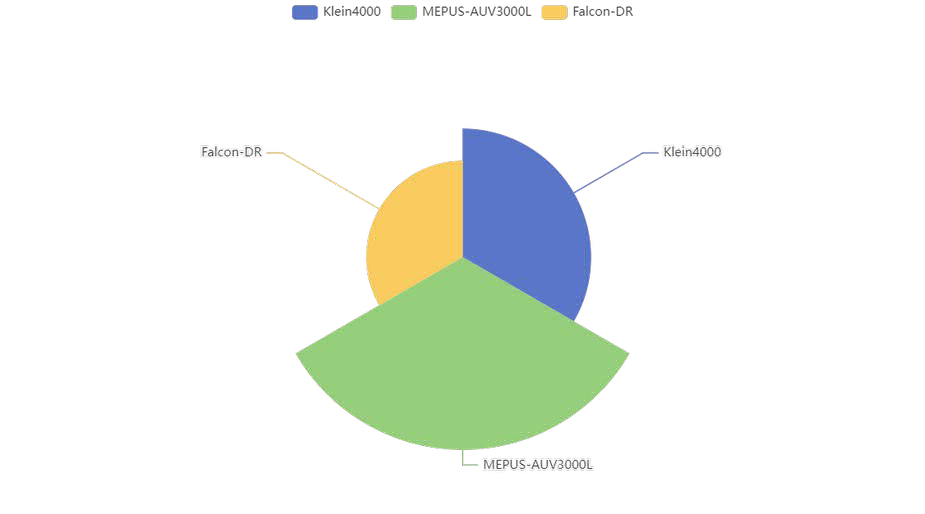
\includegraphics[width=222.15pt,height=123.4pt]{latexImage_5e4d2397b11ca38488165ddfb7368d56.png}}
\put(278,-461.411){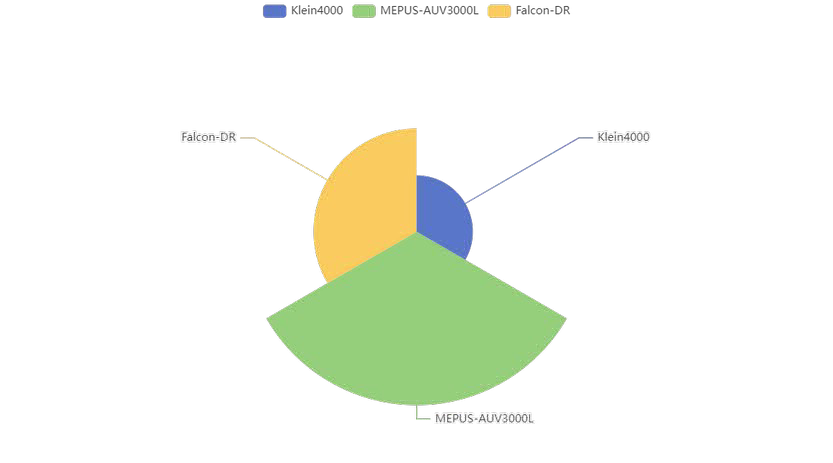
\includegraphics[width=200.25pt,height=111.25pt]{latexImage_061eafce9d4d5888363d61429d53ad68.png}}
\put(55.85,-593.061){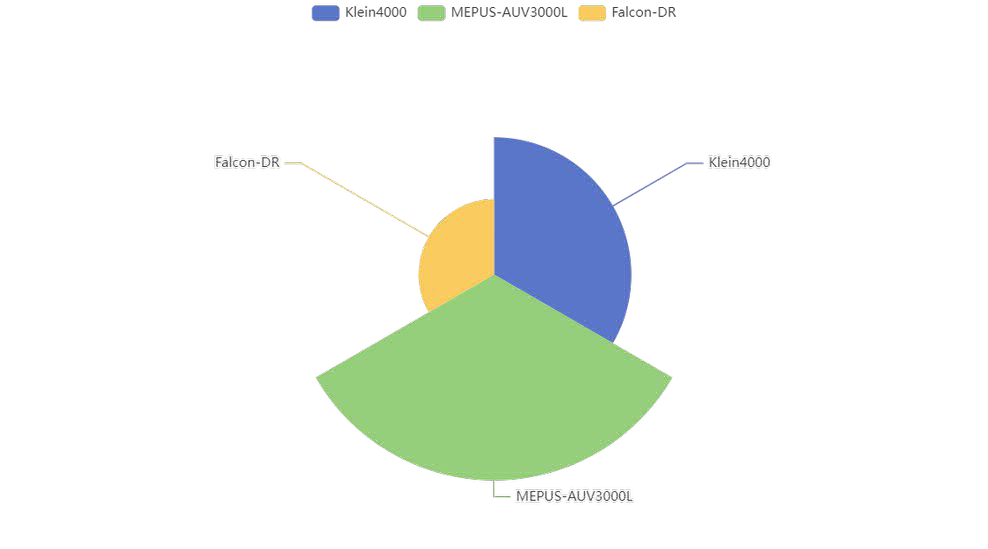
\includegraphics[width=237pt,height=131.65pt]{latexImage_f4baea2b278ec36f1193112caebfb7e0.png}}
\put(292.85,-593.061){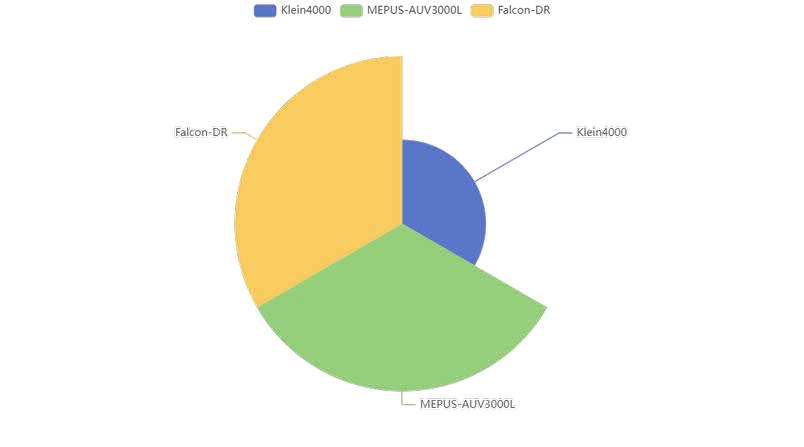
\includegraphics[width=193.2pt,height=107.3pt]{latexImage_31dcbe2348588f9d721d38b08abb260d.png}}
\put(56,-606.411){\fontsize{11}{1}\usefont{T1}{cmr}{m}{n}\selectfont\color{color_80434}图}
\put(69.2,-606.411){\fontsize{11}{1}\usefont{T1}{ptm}{m}{n}\selectfont\color{color_80434}17}
\put(80.101,-606.411){\fontsize{11}{1}\usefont{T1}{ptm}{m}{n}\selectfont\color{color_80434}.}
\put(78,-626.911){\fontsize{16}{1}\usefont{T1}{ptm}{b}{n}\selectfont\color{color_55609}3}
\put(86,-626.911){\fontsize{16}{1}\usefont{T1}{cmr}{m}{n}\selectfont\color{color_55609}、}
\put(119,-626.911){\fontsize{16}{1}\usefont{T1}{cmr}{m}{n}\selectfont\color{color_55609}模型的建立}
\end{picture}
\begin{tikzpicture}[overlay]
\path(0pt,0pt);
\filldraw[color_283006][even odd rule]
(55.9pt, -659.661pt) -- (297.85pt, -659.661pt)
 -- (297.85pt, -659.661pt)
 -- (297.85pt, -646.911pt)
 -- (297.85pt, -646.911pt)
 -- (55.9pt, -646.911pt) -- cycle
;
\end{tikzpicture}
\begin{picture}(-5,0)(2.5,0)
\put(56,-657.111){\fontsize{11}{1}\usefont{T1}{cmr}{m}{n}\selectfont\color{color_80434}假}
\put(67,-657.111){\fontsize{11}{1}\usefont{T1}{cmr}{m}{n}\selectfont\color{color_80434}设主船和救}
\put(122,-657.111){\fontsize{11}{1}\usefont{T1}{cmr}{m}{n}\selectfont\color{color_80434}援}
\put(133,-657.111){\fontsize{11}{1}\usefont{T1}{cmr}{m}{n}\selectfont\color{color_80434}船}
\put(144,-657.111){\fontsize{11}{1}\usefont{T1}{cmr}{m}{n}\selectfont\color{color_80434}总}
\put(155,-657.111){\fontsize{11}{1}\usefont{T1}{cmr}{m}{n}\selectfont\color{color_80434}共允许}
\put(188,-657.111){\fontsize{11}{1}\usefont{T1}{cmr}{m}{n}\selectfont\color{color_80434}携带设备个数}
\put(254,-657.111){\fontsize{11}{1}\usefont{T1}{cmr}{m}{n}\selectfont\color{color_80434}小}
\put(265,-657.111){\fontsize{11}{1}\usefont{T1}{cmr}{m}{n}\selectfont\color{color_80434}于等于}
\end{picture}
\begin{tikzpicture}[overlay]
\path(0pt,0pt);
\filldraw[color_283006][even odd rule]
(297.9pt, -659.661pt) -- (300.05pt, -659.661pt)
 -- (300.05pt, -659.661pt)
 -- (300.05pt, -646.911pt)
 -- (300.05pt, -646.911pt)
 -- (297.9pt, -646.911pt) -- cycle
;
\filldraw[color_283006][even odd rule]
(300.1pt, -659.461pt) -- (305.55pt, -659.461pt)
 -- (305.55pt, -659.461pt)
 -- (305.55pt, -646.811pt)
 -- (305.55pt, -646.811pt)
 -- (300.1pt, -646.811pt) -- cycle
;
\end{tikzpicture}
\begin{picture}(-5,0)(2.5,0)
\put(300.2,-657.111){\fontsize{11}{1}\usefont{T1}{ptm}{m}{n}\selectfont\color{color_80434}5}
\end{picture}
\begin{tikzpicture}[overlay]
\path(0pt,0pt);
\filldraw[color_283006][even odd rule]
(305.6pt, -659.661pt) -- (503.55pt, -659.661pt)
 -- (503.55pt, -659.661pt)
 -- (503.55pt, -646.911pt)
 -- (503.55pt, -646.911pt)
 -- (305.6pt, -646.911pt) -- cycle
;
\end{tikzpicture}
\begin{picture}(-5,0)(2.5,0)
\put(305.7,-657.111){\fontsize{11}{1}\usefont{T1}{cmr}{m}{n}\selectfont\color{color_80434},根据搜集到的设备成本和设备搜救参数}
\end{picture}
\begin{tikzpicture}[overlay]
\path(0pt,0pt);
\filldraw[color_283006][even odd rule]
(503.6pt, -659.661pt) -- (514.55pt, -659.661pt)
 -- (514.55pt, -659.661pt)
 -- (514.55pt, -646.911pt)
 -- (514.55pt, -646.911pt)
 -- (503.6pt, -646.911pt) -- cycle
;
\end{tikzpicture}
\begin{picture}(-5,0)(2.5,0)
\put(503.7,-657.111){\fontsize{11}{1}\usefont{T1}{cmr}{m}{n}\selectfont\color{color_80434},}
\end{picture}
\begin{tikzpicture}[overlay]
\path(0pt,0pt);
\filldraw[color_283006][even odd rule]
(55.9pt, -672.461pt) -- (352.85pt, -672.461pt)
 -- (352.85pt, -672.461pt)
 -- (352.85pt, -659.711pt)
 -- (352.85pt, -659.711pt)
 -- (55.9pt, -659.711pt) -- cycle
;
\end{tikzpicture}
\begin{picture}(-5,0)(2.5,0)
\put(56,-669.911){\fontsize{11}{1}\usefont{T1}{cmr}{m}{n}\selectfont\color{color_80434}我}
\put(67,-669.911){\fontsize{11}{1}\usefont{T1}{cmr}{m}{n}\selectfont\color{color_80434}们在}
\put(89,-669.911){\fontsize{11}{1}\usefont{T1}{cmr}{m}{n}\selectfont\color{color_80434}考虑}
\put(111,-669.911){\fontsize{11}{1}\usefont{T1}{cmr}{m}{n}\selectfont\color{color_80434}设备可用性的同时需要}
\put(221,-669.911){\fontsize{11}{1}\usefont{T1}{cmr}{m}{n}\selectfont\color{color_80434}尽}
\put(232,-669.911){\fontsize{11}{1}\usefont{T1}{cmr}{m}{n}\selectfont\color{color_80434}可能}
\put(254,-669.911){\fontsize{11}{1}\usefont{T1}{cmr}{m}{n}\selectfont\color{color_80434}节}
\put(265,-669.911){\fontsize{11}{1}\usefont{T1}{cmr}{m}{n}\selectfont\color{color_80434}约}
\put(276,-669.911){\fontsize{11}{1}\usefont{T1}{cmr}{m}{n}\selectfont\color{color_80434}相关的}
\put(309,-669.911){\fontsize{11}{1}\usefont{T1}{cmr}{m}{n}\selectfont\color{color_80434}开}
\put(320,-669.911){\fontsize{11}{1}\usefont{T1}{cmr}{m}{n}\selectfont\color{color_80434}支}
\put(331,-669.911){\fontsize{11}{1}\usefont{T1}{cmr}{m}{n}\selectfont\color{color_80434}成本}
\end{picture}
\begin{tikzpicture}[overlay]
\path(0pt,0pt);
\filldraw[color_283006][even odd rule]
(352.9pt, -672.261pt) -- (355.65pt, -672.261pt)
 -- (355.65pt, -672.261pt)
 -- (355.65pt, -659.711pt)
 -- (355.65pt, -659.711pt)
 -- (352.9pt, -659.711pt) -- cycle
;
\end{tikzpicture}
\begin{picture}(-5,0)(2.5,0)
\put(353,-669.911){\fontsize{11}{1}\usefont{T1}{ptm}{m}{n}\selectfont\color{color_80434}.}
\put(355.695,-669.911){\fontsize{11}{1}\usefont{T1}{ptm}{m}{n}\selectfont\color{color_80434} }
\put(358.489,-669.911){\fontsize{11}{1}\usefont{T1}{ptm}{m}{n}\selectfont\color{color_80434} }
\put(361.184,-669.911){\fontsize{11}{1}\usefont{T1}{ptm}{m}{n}\selectfont\color{color_80434} }
\put(363.978,-669.911){\fontsize{11}{1}\usefont{T1}{ptm}{m}{n}\selectfont\color{color_80434} }
\put(366.673,-669.911){\fontsize{11}{1}\usefont{T1}{ptm}{m}{n}\selectfont\color{color_80434} }
\put(369.467,-669.911){\fontsize{11}{1}\usefont{T1}{ptm}{m}{n}\selectfont\color{color_80434} }
\put(372.162,-669.911){\fontsize{11}{1}\usefont{T1}{ptm}{m}{n}\selectfont\color{color_80434} }
\put(374.9561,-669.911){\fontsize{11}{1}\usefont{T1}{ptm}{m}{n}\selectfont\color{color_80434} }
\put(377.6511,-669.911){\fontsize{11}{1}\usefont{T1}{ptm}{m}{n}\selectfont\color{color_80434} }
\put(380.4451,-669.911){\fontsize{11}{1}\usefont{T1}{ptm}{m}{n}\selectfont\color{color_80434} }
\put(383.1401,-669.911){\fontsize{11}{1}\usefont{T1}{ptm}{m}{n}\selectfont\color{color_80434} }
\put(385.9341,-669.911){\fontsize{11}{1}\usefont{T1}{ptm}{m}{n}\selectfont\color{color_80434} }
\put(388.6291,-669.911){\fontsize{11}{1}\usefont{T1}{ptm}{m}{n}\selectfont\color{color_80434} }
\put(391.4231,-669.911){\fontsize{11}{1}\usefont{T1}{ptm}{m}{n}\selectfont\color{color_80434} }
\put(394.1181,-669.911){\fontsize{11}{1}\usefont{T1}{ptm}{m}{n}\selectfont\color{color_80434} }
\put(396.9121,-669.911){\fontsize{11}{1}\usefont{T1}{ptm}{m}{n}\selectfont\color{color_80434} }
\put(399.6071,-669.911){\fontsize{11}{1}\usefont{T1}{ptm}{m}{n}\selectfont\color{color_80434} }
\put(402.4011,-669.911){\fontsize{11}{1}\usefont{T1}{ptm}{m}{n}\selectfont\color{color_80434} }
\put(405.0961,-669.911){\fontsize{11}{1}\usefont{T1}{ptm}{m}{n}\selectfont\color{color_80434} }
\end{picture}
\begin{tikzpicture}[overlay]
\path(0pt,0pt);
\filldraw[color_283006][even odd rule]
(55.9pt, -704.561pt) -- (216.85pt, -704.561pt)
 -- (216.85pt, -704.561pt)
 -- (216.85pt, -691.211pt)
 -- (216.85pt, -691.211pt)
 -- (55.9pt, -691.211pt) -- cycle
;
\end{tikzpicture}
\begin{picture}(-5,0)(2.5,0)
\put(56,-701.911){\fontsize{11.5}{1}\usefont{T1}{cmr}{m}{n}\selectfont\color{color_54684}我}
\put(67.5,-701.911){\fontsize{11.5}{1}\usefont{T1}{cmr}{m}{n}\selectfont\color{color_54684}们先建立成本效益比率模型:}
\put(56,-734.311){\fontsize{11}{1}\usefont{T1}{cmr}{m}{n}\selectfont\color{color_80434}其}
\put(67,-734.311){\fontsize{11}{1}\usefont{T1}{cmr}{m}{n}\selectfont\color{color_80434}中,}
\put(95,-734.311){\fontsize{11}{1}\usefont{T1}{cmr}{m}{n}\selectfont\color{color_80434}表}
\put(106,-734.311){\fontsize{11}{1}\usefont{T1}{cmr}{m}{n}\selectfont\color{color_80434}示}
\put(117,-734.311){\fontsize{11}{1}\usefont{T1}{cmr}{m}{n}\selectfont\color{color_80434}不同的搜索设备}
\end{picture}
\newpage
\begin{tikzpicture}[overlay]
\path(0pt,0pt);
\filldraw[color_283006][even odd rule]
(82.9pt, -77.76099pt) -- (289.85pt, -77.76099pt)
 -- (289.85pt, -77.76099pt)
 -- (289.85pt, -64.41101pt)
 -- (289.85pt, -64.41101pt)
 -- (82.9pt, -64.41101pt) -- cycle
;
\end{tikzpicture}
\begin{picture}(-5,0)(2.5,0)
\put(83,-75.11102){\fontsize{11.5}{1}\usefont{T1}{cmr}{m}{n}\selectfont\color{color_54684}表}
\put(94.5,-75.11102){\fontsize{11.5}{1}\usefont{T1}{cmr}{m}{n}\selectfont\color{color_54684}示}
\put(106,-75.11102){\fontsize{11.5}{1}\usefont{T1}{cmr}{m}{n}\selectfont\color{color_54684}设备的效益}
\put(163.5,-75.11102){\fontsize{11.5}{1}\usefont{T1}{cmr}{m}{n}\selectfont\color{color_54684}值}
\put(175,-75.11102){\fontsize{11.5}{1}\usefont{T1}{cmr}{m}{n}\selectfont\color{color_54684},可以进一}
\put(232.5,-75.11102){\fontsize{11.5}{1}\usefont{T1}{cmr}{m}{n}\selectfont\color{color_54684}步}
\put(244,-75.11102){\fontsize{11.5}{1}\usefont{T1}{cmr}{m}{n}\selectfont\color{color_54684}细}
\put(255.5,-75.11102){\fontsize{11.5}{1}\usefont{T1}{cmr}{m}{n}\selectfont\color{color_54684}化为:}
\end{picture}
\begin{tikzpicture}[overlay]
\path(0pt,0pt);
\filldraw[color_283006][even odd rule]
(55.9pt, -145.661pt) -- (78.85001pt, -145.661pt)
 -- (78.85001pt, -145.661pt)
 -- (78.85001pt, -132.311pt)
 -- (78.85001pt, -132.311pt)
 -- (55.9pt, -132.311pt) -- cycle
;
\end{tikzpicture}
\begin{picture}(-5,0)(2.5,0)
\put(56,-143.011){\fontsize{11.5}{1}\usefont{T1}{cmr}{m}{n}\selectfont\color{color_54684}其}
\put(67.5,-143.011){\fontsize{11.5}{1}\usefont{T1}{cmr}{m}{n}\selectfont\color{color_54684}中}
\end{picture}
\begin{tikzpicture}[overlay]
\path(0pt,0pt);
\filldraw[color_283006][even odd rule]
(135.9pt, -145.661pt) -- (204.85pt, -145.661pt)
 -- (204.85pt, -145.661pt)
 -- (204.85pt, -132.311pt)
 -- (204.85pt, -132.311pt)
 -- (135.9pt, -132.311pt) -- cycle
;
\end{tikzpicture}
\begin{picture}(-5,0)(2.5,0)
\put(136,-143.011){\fontsize{11.5}{1}\usefont{T1}{cmr}{m}{n}\selectfont\color{color_54684}是}
\put(147.5,-143.011){\fontsize{11.5}{1}\usefont{T1}{cmr}{m}{n}\selectfont\color{color_54684}搜索}
\put(170.5,-143.011){\fontsize{11.5}{1}\usefont{T1}{cmr}{m}{n}\selectfont\color{color_54684}深度}
\put(193.5,-143.011){\fontsize{11.5}{1}\usefont{T1}{cmr}{m}{n}\selectfont\color{color_54684},}
\end{picture}
\begin{tikzpicture}[overlay]
\path(0pt,0pt);
\filldraw[color_283006][even odd rule]
(243.2pt, -145.661pt) -- (312.15pt, -145.661pt)
 -- (312.15pt, -145.661pt)
 -- (312.15pt, -132.311pt)
 -- (312.15pt, -132.311pt)
 -- (243.2pt, -132.311pt) -- cycle
;
\end{tikzpicture}
\begin{picture}(-5,0)(2.5,0)
\put(243.3,-143.011){\fontsize{11.5}{1}\usefont{T1}{cmr}{m}{n}\selectfont\color{color_54684}是}
\put(254.8,-143.011){\fontsize{11.5}{1}\usefont{T1}{cmr}{m}{n}\selectfont\color{color_54684}搜索}
\put(277.8,-143.011){\fontsize{11.5}{1}\usefont{T1}{cmr}{m}{n}\selectfont\color{color_54684}范围}
\put(300.8,-143.011){\fontsize{11.5}{1}\usefont{T1}{cmr}{m}{n}\selectfont\color{color_54684},}
\end{picture}
\begin{tikzpicture}[overlay]
\path(0pt,0pt);
\filldraw[color_283006][even odd rule]
(348.3pt, -145.661pt) -- (405.75pt, -145.661pt)
 -- (405.75pt, -145.661pt)
 -- (405.75pt, -132.311pt)
 -- (405.75pt, -132.311pt)
 -- (348.3pt, -132.311pt) -- cycle
;
\end{tikzpicture}
\begin{picture}(-5,0)(2.5,0)
\put(348.4,-143.011){\fontsize{11.5}{1}\usefont{T1}{cmr}{m}{n}\selectfont\color{color_54684}是}
\put(359.9,-143.011){\fontsize{11.5}{1}\usefont{T1}{cmr}{m}{n}\selectfont\color{color_54684}搜索}
\put(382.9,-143.011){\fontsize{11.5}{1}\usefont{T1}{cmr}{m}{n}\selectfont\color{color_54684}速度}
\end{picture}
\begin{tikzpicture}[overlay]
\path(0pt,0pt);
\filldraw[color_283006][even odd rule]
(405.8pt, -145.661pt) -- (409.45pt, -145.661pt)
 -- (409.45pt, -145.661pt)
 -- (409.45pt, -132.311pt)
 -- (409.45pt, -132.311pt)
 -- (405.8pt, -132.311pt) -- cycle
;
\end{tikzpicture}
\begin{picture}(-5,0)(2.5,0)
\put(405.9,-143.011){\fontsize{11.5}{1}\usefont{T1}{cmr}{m}{n}\selectfont\color{color_54684}.}
\end{picture}
\begin{tikzpicture}[overlay]
\path(0pt,0pt);
\filldraw[color_283006][even odd rule]
(55.9pt, -178.461pt) -- (62.85pt, -178.461pt)
 -- (62.85pt, -178.461pt)
 -- (62.85pt, -165.111pt)
 -- (62.85pt, -165.111pt)
 -- (55.9pt, -165.111pt) -- cycle
;
\end{tikzpicture}
\begin{picture}(-5,0)(2.5,0)
\put(56,-175.811){\fontsize{11.5}{1}\usefont{T1}{cmr}{m}{n}\selectfont\color{color_54684}a}
\end{picture}
\begin{tikzpicture}[overlay]
\path(0pt,0pt);
\filldraw[color_283006][even odd rule]
(62.9pt, -178.461pt) -- (74.35pt, -178.461pt)
 -- (74.35pt, -178.461pt)
 -- (74.35pt, -165.111pt)
 -- (74.35pt, -165.111pt)
 -- (62.9pt, -165.111pt) -- cycle
;
\end{tikzpicture}
\begin{picture}(-5,0)(2.5,0)
\put(63,-175.811){\fontsize{11.5}{1}\usefont{T1}{cmr}{m}{n}\selectfont\color{color_54684}、}
\end{picture}
\begin{tikzpicture}[overlay]
\path(0pt,0pt);
\filldraw[color_283006][even odd rule]
(74.4pt, -178.461pt) -- (81.65pt, -178.461pt)
 -- (81.65pt, -178.461pt)
 -- (81.65pt, -165.111pt)
 -- (81.65pt, -165.111pt)
 -- (74.4pt, -165.111pt) -- cycle
;
\end{tikzpicture}
\begin{picture}(-5,0)(2.5,0)
\put(74.5,-175.811){\fontsize{11.5}{1}\usefont{T1}{cmr}{m}{n}\selectfont\color{color_54684}b}
\end{picture}
\begin{tikzpicture}[overlay]
\path(0pt,0pt);
\filldraw[color_283006][even odd rule]
(81.7pt, -178.461pt) -- (93.14999pt, -178.461pt)
 -- (93.14999pt, -178.461pt)
 -- (93.14999pt, -165.111pt)
 -- (93.14999pt, -165.111pt)
 -- (81.7pt, -165.111pt) -- cycle
;
\end{tikzpicture}
\begin{picture}(-5,0)(2.5,0)
\put(81.8,-175.811){\fontsize{11.5}{1}\usefont{T1}{cmr}{m}{n}\selectfont\color{color_54684}、}
\end{picture}
\begin{tikzpicture}[overlay]
\path(0pt,0pt);
\filldraw[color_283006][even odd rule]
(93.2pt, -178.461pt) -- (99.55pt, -178.461pt)
 -- (99.55pt, -178.461pt)
 -- (99.55pt, -165.111pt)
 -- (99.55pt, -165.111pt)
 -- (93.2pt, -165.111pt) -- cycle
;
\end{tikzpicture}
\begin{picture}(-5,0)(2.5,0)
\put(93.3,-175.811){\fontsize{11.5}{1}\usefont{T1}{cmr}{m}{n}\selectfont\color{color_54684}c}
\end{picture}
\begin{tikzpicture}[overlay]
\path(0pt,0pt);
\filldraw[color_283006][even odd rule]
(99.6pt, -178.461pt) -- (101.85pt, -178.461pt)
 -- (101.85pt, -178.461pt)
 -- (101.85pt, -165.111pt)
 -- (101.85pt, -165.111pt)
 -- (99.6pt, -165.111pt) -- cycle
;
\filldraw[color_283006][even odd rule]
(101.9pt, -178.461pt) -- (193.85pt, -178.461pt)
 -- (193.85pt, -178.461pt)
 -- (193.85pt, -165.111pt)
 -- (193.85pt, -165.111pt)
 -- (101.9pt, -165.111pt) -- cycle
;
\end{tikzpicture}
\begin{picture}(-5,0)(2.5,0)
\put(102,-175.811){\fontsize{11.5}{1}\usefont{T1}{cmr}{m}{n}\selectfont\color{color_54684}为这些因素的权重}
\end{picture}
\begin{tikzpicture}[overlay]
\path(0pt,0pt);
\filldraw[color_283006][even odd rule]
(55.9pt, -211.261pt) -- (79.95pt, -211.261pt)
 -- (79.95pt, -211.261pt)
 -- (79.95pt, -197.911pt)
 -- (79.95pt, -197.911pt)
 -- (55.9pt, -197.911pt) -- cycle
;
\end{tikzpicture}
\begin{picture}(-5,0)(2.5,0)
\put(56,-208.611){\fontsize{11.5}{1}\usefont{T1}{cmr}{m}{n}\selectfont\color{color_54684}C}
\put(64.004,-208.611){\fontsize{11.5}{1}\usefont{T1}{cmr}{m}{n}\selectfont\color{color_54684}(e}
\put(75.573,-208.611){\fontsize{11.5}{1}\usefont{T1}{cmr}{m}{n}\selectfont\color{color_54684})}
\end{picture}
\begin{tikzpicture}[overlay]
\path(0pt,0pt);
\filldraw[color_283006][even odd rule]
(80pt, -211.261pt) -- (286.95pt, -211.261pt)
 -- (286.95pt, -211.261pt)
 -- (286.95pt, -197.911pt)
 -- (286.95pt, -197.911pt)
 -- (80pt, -197.911pt) -- cycle
;
\end{tikzpicture}
\begin{picture}(-5,0)(2.5,0)
\put(80.1,-208.611){\fontsize{11.5}{1}\usefont{T1}{cmr}{m}{n}\selectfont\color{color_54684}表}
\put(91.6,-208.611){\fontsize{11.5}{1}\usefont{T1}{cmr}{m}{n}\selectfont\color{color_54684}示}
\put(103.1,-208.611){\fontsize{11.5}{1}\usefont{T1}{cmr}{m}{n}\selectfont\color{color_54684}设备的}
\put(137.6,-208.611){\fontsize{11.5}{1}\usefont{T1}{cmr}{m}{n}\selectfont\color{color_54684}总}
\put(149.1,-208.611){\fontsize{11.5}{1}\usefont{T1}{cmr}{m}{n}\selectfont\color{color_54684}成本,可以进一}
\put(229.6,-208.611){\fontsize{11.5}{1}\usefont{T1}{cmr}{m}{n}\selectfont\color{color_54684}步}
\put(241.1,-208.611){\fontsize{11.5}{1}\usefont{T1}{cmr}{m}{n}\selectfont\color{color_54684}细}
\put(252.6,-208.611){\fontsize{11.5}{1}\usefont{T1}{cmr}{m}{n}\selectfont\color{color_54684}化为:}
\put(56,-276.411){\fontsize{11}{1}\usefont{T1}{cmr}{m}{n}\selectfont\color{color_80434}其}
\put(67,-276.411){\fontsize{11}{1}\usefont{T1}{cmr}{m}{n}\selectfont\color{color_80434}中}
\put(134.3,-276.411){\fontsize{11}{1}\usefont{T1}{cmr}{m}{n}\selectfont\color{color_80434}是}
\put(145.3,-276.411){\fontsize{11}{1}\usefont{T1}{cmr}{m}{n}\selectfont\color{color_80434}设备成本,}
\put(246.1,-276.411){\fontsize{11}{1}\usefont{T1}{cmr}{m}{n}\selectfont\color{color_80434}是人员培训}
\put(301.1,-276.411){\fontsize{11}{1}\usefont{T1}{cmr}{m}{n}\selectfont\color{color_80434}成本,}
\put(376.1,-276.411){\fontsize{11}{1}\usefont{T1}{cmr}{m}{n}\selectfont\color{color_80434}是储}
\put(398.1,-276.411){\fontsize{11}{1}\usefont{T1}{cmr}{m}{n}\selectfont\color{color_80434}存与}
\put(420.1,-276.411){\fontsize{11}{1}\usefont{T1}{cmr}{m}{n}\selectfont\color{color_80434}保养}
\put(442.1,-276.411){\fontsize{11}{1}\usefont{T1}{cmr}{m}{n}\selectfont\color{color_80434}成本}
\put(464.1,-276.411){\fontsize{11}{1}\usefont{T1}{ptm}{m}{n}\selectfont\color{color_80434}.}
\put(78,-297.011){\fontsize{16}{1}\usefont{T1}{ptm}{b}{n}\selectfont\color{color_55609}4}
\put(86,-297.011){\fontsize{16}{1}\usefont{T1}{cmr}{m}{n}\selectfont\color{color_55609}、}
\put(119,-297.011){\fontsize{16}{1}\usefont{T1}{cmr}{m}{n}\selectfont\color{color_55609}模型的}
\put(167,-297.011){\fontsize{16}{1}\usefont{T1}{cmr}{m}{n}\selectfont\color{color_55609}求解}
\end{picture}
\begin{tikzpicture}[overlay]
\path(0pt,0pt);
\filldraw[color_283006][even odd rule]
(55.9pt, -329.661pt) -- (165.85pt, -329.661pt)
 -- (165.85pt, -329.661pt)
 -- (165.85pt, -316.911pt)
 -- (165.85pt, -316.911pt)
 -- (55.9pt, -316.911pt) -- cycle
;
\end{tikzpicture}
\begin{picture}(-5,0)(2.5,0)
\put(56,-327.111){\fontsize{11}{1}\usefont{T1}{cmr}{m}{n}\selectfont\color{color_80434}根据数据}
\put(100,-327.111){\fontsize{11}{1}\usefont{T1}{cmr}{m}{n}\selectfont\color{color_80434}我}
\put(111,-327.111){\fontsize{11}{1}\usefont{T1}{cmr}{m}{n}\selectfont\color{color_80434}们可以}
\put(144,-327.111){\fontsize{11}{1}\usefont{T1}{cmr}{m}{n}\selectfont\color{color_80434}列}
\put(155,-327.111){\fontsize{11}{1}\usefont{T1}{cmr}{m}{n}\selectfont\color{color_80434}出}
\end{picture}
\begin{tikzpicture}[overlay]
\path(0pt,0pt);
\filldraw[color_283006][even odd rule]
(165.9pt, -329.461pt) -- (168.95pt, -329.461pt)
 -- (168.95pt, -329.461pt)
 -- (168.95pt, -316.911pt)
 -- (168.95pt, -316.911pt)
 -- (165.9pt, -316.911pt) -- cycle
;
\end{tikzpicture}
\begin{picture}(-5,0)(2.5,0)
\put(166,-327.111){\fontsize{11}{1}\usefont{T1}{ptm}{m}{n}\selectfont\color{color_80434}:}
\end{picture}
\newpage
\begin{tikzpicture}[overlay]
\path(0pt,0pt);
\filldraw[color_283006][even odd rule]
(55.9pt, -118.161pt) -- (396.85pt, -118.161pt)
 -- (396.85pt, -118.161pt)
 -- (396.85pt, -105.411pt)
 -- (396.85pt, -105.411pt)
 -- (55.9pt, -105.411pt) -- cycle
;
\end{tikzpicture}
\begin{picture}(-5,0)(2.5,0)
\put(56,-115.611){\fontsize{11}{1}\usefont{T1}{cmr}{m}{n}\selectfont\color{color_80434}对于}
\put(78,-115.611){\fontsize{11}{1}\usefont{T1}{cmr}{m}{n}\selectfont\color{color_80434}线}
\put(89,-115.611){\fontsize{11}{1}\usefont{T1}{cmr}{m}{n}\selectfont\color{color_80434}性}
\put(100,-115.611){\fontsize{11}{1}\usefont{T1}{cmr}{m}{n}\selectfont\color{color_80434}整}
\put(111,-115.611){\fontsize{11}{1}\usefont{T1}{cmr}{m}{n}\selectfont\color{color_80434}数}
\put(122,-115.611){\fontsize{11}{1}\usefont{T1}{cmr}{m}{n}\selectfont\color{color_80434}规}
\put(133,-115.611){\fontsize{11}{1}\usefont{T1}{cmr}{m}{n}\selectfont\color{color_80434}划问题,}
\put(177,-115.611){\fontsize{11}{1}\usefont{T1}{cmr}{m}{n}\selectfont\color{color_80434}我}
\put(188,-115.611){\fontsize{11}{1}\usefont{T1}{cmr}{m}{n}\selectfont\color{color_80434}们可以}
\put(221,-115.611){\fontsize{11}{1}\usefont{T1}{cmr}{m}{n}\selectfont\color{color_80434}采}
\put(232,-115.611){\fontsize{11}{1}\usefont{T1}{cmr}{m}{n}\selectfont\color{color_80434}用}
\put(243,-115.611){\fontsize{11}{1}\usefont{T1}{cmr}{m}{n}\selectfont\color{color_80434}蒙}
\put(254,-115.611){\fontsize{11}{1}\usefont{T1}{cmr}{m}{n}\selectfont\color{color_80434}特}
\put(265,-115.611){\fontsize{11}{1}\usefont{T1}{cmr}{m}{n}\selectfont\color{color_80434}卡洛}
\put(287,-115.611){\fontsize{11}{1}\usefont{T1}{cmr}{m}{n}\selectfont\color{color_80434}法进行}
\put(320,-115.611){\fontsize{11}{1}\usefont{T1}{cmr}{m}{n}\selectfont\color{color_80434}估}
\put(331,-115.611){\fontsize{11}{1}\usefont{T1}{cmr}{m}{n}\selectfont\color{color_80434}算,}
\put(353,-115.611){\fontsize{11}{1}\usefont{T1}{cmr}{m}{n}\selectfont\color{color_80434}我}
\put(364,-115.611){\fontsize{11}{1}\usefont{T1}{cmr}{m}{n}\selectfont\color{color_80434}们}
\put(375,-115.611){\fontsize{11}{1}\usefont{T1}{cmr}{m}{n}\selectfont\color{color_80434}假}
\put(386,-115.611){\fontsize{11}{1}\usefont{T1}{cmr}{m}{n}\selectfont\color{color_80434}设}
\end{picture}
\begin{tikzpicture}[overlay]
\path(0pt,0pt);
\filldraw[color_283006][even odd rule]
(427.7pt, -118.161pt) -- (460.65pt, -118.161pt)
 -- (460.65pt, -118.161pt)
 -- (460.65pt, -105.411pt)
 -- (460.65pt, -105.411pt)
 -- (427.7pt, -105.411pt) -- cycle
;
\end{tikzpicture}
\begin{picture}(-5,0)(2.5,0)
\put(427.8,-115.611){\fontsize{11}{1}\usefont{T1}{cmr}{m}{n}\selectfont\color{color_80434}分}
\put(438.8,-115.611){\fontsize{11}{1}\usefont{T1}{cmr}{m}{n}\selectfont\color{color_80434}别}
\put(449.8,-115.611){\fontsize{11}{1}\usefont{T1}{cmr}{m}{n}\selectfont\color{color_80434}为}
\end{picture}
\begin{tikzpicture}[overlay]
\path(0pt,0pt);
\filldraw[color_283006][even odd rule]
(55.9pt, -130.761pt) -- (69.55pt, -130.761pt)
 -- (69.55pt, -130.761pt)
 -- (69.55pt, -118.211pt)
 -- (69.55pt, -118.211pt)
 -- (55.9pt, -118.211pt) -- cycle
;
\end{tikzpicture}
\begin{picture}(-5,0)(2.5,0)
\put(56,-128.411){\fontsize{11}{1}\usefont{T1}{ptm}{m}{n}\selectfont\color{color_80434}0}
\put(61.401,-128.411){\fontsize{11}{1}\usefont{T1}{ptm}{m}{n}\selectfont\color{color_80434}.}
\put(64.195,-128.411){\fontsize{11}{1}\usefont{T1}{ptm}{m}{n}\selectfont\color{color_80434}4}
\end{picture}
\begin{tikzpicture}[overlay]
\path(0pt,0pt);
\filldraw[color_283006][even odd rule]
(69.6pt, -130.961pt) -- (80.55pt, -130.961pt)
 -- (80.55pt, -130.961pt)
 -- (80.55pt, -118.211pt)
 -- (80.55pt, -118.211pt)
 -- (69.6pt, -118.211pt) -- cycle
;
\end{tikzpicture}
\begin{picture}(-5,0)(2.5,0)
\put(69.7,-128.411){\fontsize{11}{1}\usefont{T1}{cmr}{m}{n}\selectfont\color{color_80434},}
\end{picture}
\begin{tikzpicture}[overlay]
\path(0pt,0pt);
\filldraw[color_283006][even odd rule]
(80.6pt, -130.761pt) -- (94.35pt, -130.761pt)
 -- (94.35pt, -130.761pt)
 -- (94.35pt, -118.211pt)
 -- (94.35pt, -118.211pt)
 -- (80.6pt, -118.211pt) -- cycle
;
\end{tikzpicture}
\begin{picture}(-5,0)(2.5,0)
\put(80.7,-128.411){\fontsize{11}{1}\usefont{T1}{ptm}{m}{n}\selectfont\color{color_80434}0.}
\put(88.994,-128.411){\fontsize{11}{1}\usefont{T1}{ptm}{m}{n}\selectfont\color{color_80434}3}
\end{picture}
\begin{tikzpicture}[overlay]
\path(0pt,0pt);
\filldraw[color_283006][even odd rule]
(94.4pt, -130.961pt) -- (105.35pt, -130.961pt)
 -- (105.35pt, -130.961pt)
 -- (105.35pt, -118.211pt)
 -- (105.35pt, -118.211pt)
 -- (94.4pt, -118.211pt) -- cycle
;
\end{tikzpicture}
\begin{picture}(-5,0)(2.5,0)
\put(94.5,-128.411){\fontsize{11}{1}\usefont{T1}{cmr}{m}{n}\selectfont\color{color_80434},}
\end{picture}
\begin{tikzpicture}[overlay]
\path(0pt,0pt);
\filldraw[color_283006][even odd rule]
(105.4pt, -130.761pt) -- (124.55pt, -130.761pt)
 -- (124.55pt, -130.761pt)
 -- (124.55pt, -118.211pt)
 -- (124.55pt, -118.211pt)
 -- (105.4pt, -118.211pt) -- cycle
;
\end{tikzpicture}
\begin{picture}(-5,0)(2.5,0)
\put(105.5,-128.411){\fontsize{11}{1}\usefont{T1}{ptm}{m}{n}\selectfont\color{color_80434}0}
\put(110.901,-128.411){\fontsize{11}{1}\usefont{T1}{ptm}{m}{n}\selectfont\color{color_80434}.}
\put(113.695,-128.411){\fontsize{11}{1}\usefont{T1}{ptm}{m}{n}\selectfont\color{color_80434}3 }
\put(121.989,-128.411){\fontsize{11}{1}\usefont{T1}{ptm}{m}{n}\selectfont\color{color_80434} }
\end{picture}
\begin{tikzpicture}[overlay]
\path(0pt,0pt);
\filldraw[color_283006][even odd rule]
(124.6pt, -130.961pt) -- (256.55pt, -130.961pt)
 -- (256.55pt, -130.961pt)
 -- (256.55pt, -118.211pt)
 -- (256.55pt, -118.211pt)
 -- (124.6pt, -118.211pt) -- cycle
;
\end{tikzpicture}
\begin{picture}(-5,0)(2.5,0)
\put(124.7,-128.411){\fontsize{11}{1}\usefont{T1}{cmr}{m}{n}\selectfont\color{color_80434},}
\put(135.7,-128.411){\fontsize{11}{1}\usefont{T1}{cmr}{m}{n}\selectfont\color{color_80434}然}
\put(146.7,-128.411){\fontsize{11}{1}\usefont{T1}{cmr}{m}{n}\selectfont\color{color_80434}后}
\put(157.7,-128.411){\fontsize{11}{1}\usefont{T1}{cmr}{m}{n}\selectfont\color{color_80434}我}
\put(168.7,-128.411){\fontsize{11}{1}\usefont{T1}{cmr}{m}{n}\selectfont\color{color_80434}们}
\put(179.7,-128.411){\fontsize{11}{1}\usefont{T1}{cmr}{m}{n}\selectfont\color{color_80434}继续}
\put(201.7,-128.411){\fontsize{11}{1}\usefont{T1}{cmr}{m}{n}\selectfont\color{color_80434}进行分析:}
\end{picture}
\begin{tikzpicture}[overlay]
\path(0pt,0pt);
\filldraw[color_283006][even odd rule]
(55.9pt, -294.561pt) -- (125.75pt, -294.561pt)
 -- (125.75pt, -294.561pt)
 -- (125.75pt, -281.811pt)
 -- (125.75pt, -281.811pt)
 -- (55.9pt, -281.811pt) -- cycle
;
\end{tikzpicture}
\begin{picture}(-5,0)(2.5,0)
\put(56,-292.011){\fontsize{11}{1}\usefont{T1}{cmr}{m}{n}\selectfont\color{color_80434}对}
\put(67.594,-292.011){\fontsize{11}{1}\usefont{T1}{cmr}{m}{n}\selectfont\color{color_80434}设}
\put(79.287,-292.011){\fontsize{11}{1}\usefont{T1}{cmr}{m}{n}\selectfont\color{color_80434}备}
\put(90.9,-292.011){\fontsize{11}{1}\usefont{T1}{cmr}{m}{n}\selectfont\color{color_80434}总}
\put(102.6,-292.011){\fontsize{11}{1}\usefont{T1}{cmr}{m}{n}\selectfont\color{color_80434}成}
\put(114.194,-292.011){\fontsize{11}{1}\usefont{T1}{cmr}{m}{n}\selectfont\color{color_80434}本}
\end{picture}
\begin{tikzpicture}[overlay]
\path(0pt,0pt);
\filldraw[color_283006][even odd rule]
(152.9pt, -294.561pt) -- (269.45pt, -294.561pt)
 -- (269.45pt, -294.561pt)
 -- (269.45pt, -281.811pt)
 -- (269.45pt, -281.811pt)
 -- (152.9pt, -281.811pt) -- cycle
;
\end{tikzpicture}
\begin{picture}(-5,0)(2.5,0)
\put(153,-292.011){\fontsize{11}{1}\usefont{T1}{cmr}{m}{n}\selectfont\color{color_80434}使}
\put(164.594,-292.011){\fontsize{11}{1}\usefont{T1}{cmr}{m}{n}\selectfont\color{color_80434}用}
\put(176.3,-292.011){\fontsize{11}{1}\usefont{T1}{cmr}{m}{n}\selectfont\color{color_80434}蒙}
\put(187.9,-292.011){\fontsize{11}{1}\usefont{T1}{cmr}{m}{n}\selectfont\color{color_80434}特}
\put(199.6,-292.011){\fontsize{11}{1}\usefont{T1}{cmr}{m}{n}\selectfont\color{color_80434}卡}
\put(211.194,-292.011){\fontsize{11}{1}\usefont{T1}{cmr}{m}{n}\selectfont\color{color_80434}洛}
\put(222.9,-292.011){\fontsize{11}{1}\usefont{T1}{cmr}{m}{n}\selectfont\color{color_80434}算}
\put(234.494,-292.011){\fontsize{11}{1}\usefont{T1}{cmr}{m}{n}\selectfont\color{color_80434}法}
\put(246.187,-292.011){\fontsize{11}{1}\usefont{T1}{cmr}{m}{n}\selectfont\color{color_80434}模}
\put(257.781,-292.011){\fontsize{11}{1}\usefont{T1}{cmr}{m}{n}\selectfont\color{color_80434}拟}
\end{picture}
\begin{tikzpicture}[overlay]
\path(0pt,0pt);
\filldraw[color_283006][even odd rule]
(269.5pt, -294.561pt) -- (271.65pt, -294.561pt)
 -- (271.65pt, -294.561pt)
 -- (271.65pt, -281.811pt)
 -- (271.65pt, -281.811pt)
 -- (269.5pt, -281.811pt) -- cycle
;
\filldraw[color_283006][even odd rule]
(271.7pt, -294.361pt) -- (294.25pt, -294.361pt)
 -- (294.25pt, -294.361pt)
 -- (294.25pt, -281.811pt)
 -- (294.25pt, -281.811pt)
 -- (271.7pt, -281.811pt) -- cycle
;
\end{tikzpicture}
\begin{picture}(-5,0)(2.5,0)
\put(271.8,-292.011){\fontsize{11}{1}\usefont{T1}{ptm}{m}{n}\selectfont\color{color_80434}1000}
\end{picture}
\begin{tikzpicture}[overlay]
\path(0pt,0pt);
\filldraw[color_283006][even odd rule]
(294.3pt, -294.361pt) -- (296.45pt, -294.361pt)
 -- (296.45pt, -294.361pt)
 -- (296.45pt, -281.811pt)
 -- (296.45pt, -281.811pt)
 -- (294.3pt, -281.811pt) -- cycle
;
\filldraw[color_283006][even odd rule]
(296.5pt, -294.561pt) -- (424.75pt, -294.561pt)
 -- (424.75pt, -294.561pt)
 -- (424.75pt, -281.811pt)
 -- (424.75pt, -281.811pt)
 -- (296.5pt, -281.811pt) -- cycle
;
\end{tikzpicture}
\begin{picture}(-5,0)(2.5,0)
\put(296.6,-292.011){\fontsize{11}{1}\usefont{T1}{cmr}{m}{n}\selectfont\color{color_80434}次}
\put(308.3,-292.011){\fontsize{11}{1}\usefont{T1}{cmr}{m}{n}\selectfont\color{color_80434}后}
\put(319.894,-292.011){\fontsize{11}{1}\usefont{T1}{cmr}{m}{n}\selectfont\color{color_80434}得}
\put(331.587,-292.011){\fontsize{11}{1}\usefont{T1}{cmr}{m}{n}\selectfont\color{color_80434}到}
\put(343.181,-292.011){\fontsize{11}{1}\usefont{T1}{cmr}{m}{n}\selectfont\color{color_80434}下}
\put(354.9,-292.011){\fontsize{11}{1}\usefont{T1}{cmr}{m}{n}\selectfont\color{color_80434}图}
\put(366.5,-292.011){\fontsize{11}{1}\usefont{T1}{cmr}{m}{n}\selectfont\color{color_80434},}
\put(378.193,-292.011){\fontsize{11}{1}\usefont{T1}{cmr}{m}{n}\selectfont\color{color_80434}不}
\put(389.8,-292.011){\fontsize{11}{1}\usefont{T1}{cmr}{m}{n}\selectfont\color{color_80434}难}
\put(401.493,-292.011){\fontsize{11}{1}\usefont{T1}{cmr}{m}{n}\selectfont\color{color_80434}看}
\put(413.1,-292.011){\fontsize{11}{1}\usefont{T1}{cmr}{m}{n}\selectfont\color{color_80434}出}
\end{picture}
\begin{tikzpicture}[overlay]
\path(0pt,0pt);
\filldraw[color_283006][even odd rule]
(451.8pt, -294.561pt) -- (509.35pt, -294.561pt)
 -- (509.35pt, -294.561pt)
 -- (509.35pt, -281.811pt)
 -- (509.35pt, -281.811pt)
 -- (451.8pt, -281.811pt) -- cycle
;
\end{tikzpicture}
\begin{picture}(-5,0)(2.5,0)
\put(451.9,-292.011){\fontsize{11}{1}\usefont{T1}{cmr}{m}{n}\selectfont\color{color_80434}大}
\put(463.6,-292.011){\fontsize{11}{1}\usefont{T1}{cmr}{m}{n}\selectfont\color{color_80434}多}
\put(475.194,-292.011){\fontsize{11}{1}\usefont{T1}{cmr}{m}{n}\selectfont\color{color_80434}分}
\put(486.887,-292.011){\fontsize{11}{1}\usefont{T1}{cmr}{m}{n}\selectfont\color{color_80434}布}
\put(498.481,-292.011){\fontsize{11}{1}\usefont{T1}{cmr}{m}{n}\selectfont\color{color_80434}在}
\end{picture}
\begin{tikzpicture}[overlay]
\path(0pt,0pt);
\filldraw[color_283006][even odd rule]
(55.9pt, -307.261pt) -- (114.45pt, -307.261pt)
 -- (114.45pt, -307.261pt)
 -- (114.45pt, -294.611pt)
 -- (114.45pt, -294.611pt)
 -- (55.9pt, -294.611pt) -- cycle
;
\end{tikzpicture}
\begin{picture}(-5,0)(2.5,0)
\put(56,-304.911){\fontsize{11}{1}\usefont{T1}{ptm}{m}{n}\selectfont\color{color_80434}60000}
\put(83.401,-304.911){\fontsize{11}{1}\usefont{T1}{ptm}{m}{n}\selectfont\color{color_80434}-}
\put(87.086,-304.911){\fontsize{11}{1}\usefont{T1}{ptm}{m}{n}\selectfont\color{color_80434}80000}
\end{picture}
\begin{tikzpicture}[overlay]
\path(0pt,0pt);
\filldraw[color_283006][even odd rule]
(114.5pt, -307.261pt) -- (116.65pt, -307.261pt)
 -- (116.65pt, -307.261pt)
 -- (116.65pt, -294.611pt)
 -- (116.65pt, -294.611pt)
 -- (114.5pt, -294.611pt) -- cycle
;
\filldraw[color_283006][even odd rule]
(116.7pt, -307.461pt) -- (171.65pt, -307.461pt)
 -- (171.65pt, -307.461pt)
 -- (171.65pt, -294.711pt)
 -- (171.65pt, -294.711pt)
 -- (116.7pt, -294.711pt) -- cycle
;
\end{tikzpicture}
\begin{picture}(-5,0)(2.5,0)
\put(116.8,-304.911){\fontsize{11}{1}\usefont{T1}{cmr}{m}{n}\selectfont\color{color_80434}区间}
\put(138.8,-304.911){\fontsize{11}{1}\usefont{T1}{cmr}{m}{n}\selectfont\color{color_80434}范围内}
\put(130.25,-542.761){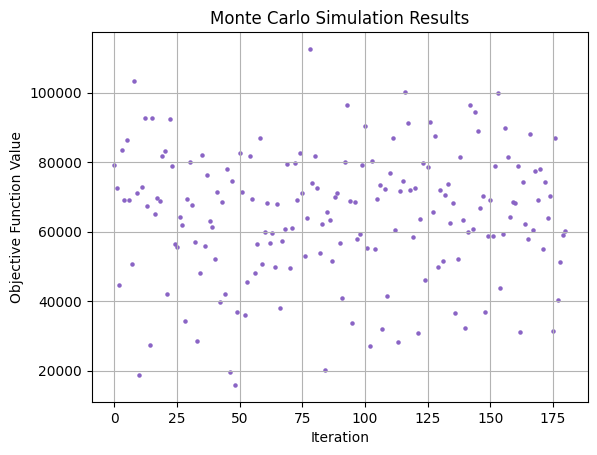
\includegraphics[width=304.85pt,height=232.35pt]{latexImage_1f4ec95f72a0dd96b5e2f6074f2cca0e.png}}
\end{picture}
\begin{tikzpicture}[overlay]
\path(0pt,0pt);
\filldraw[color_283006][even odd rule]
(55.9pt, -561.961pt) -- (121.85pt, -561.961pt)
 -- (121.85pt, -561.961pt)
 -- (121.85pt, -549.211pt)
 -- (121.85pt, -549.211pt)
 -- (55.9pt, -549.211pt) -- cycle
;
\end{tikzpicture}
\begin{picture}(-5,0)(2.5,0)
\put(56,-559.411){\fontsize{11}{1}\usefont{T1}{cmr}{m}{n}\selectfont\color{color_80434}对设备效益}
\put(111,-559.411){\fontsize{11}{1}\usefont{T1}{cmr}{m}{n}\selectfont\color{color_80434}值}
\end{picture}
\begin{tikzpicture}[overlay]
\path(0pt,0pt);
\filldraw[color_283006][even odd rule]
(148.9pt, -561.961pt) -- (258.85pt, -561.961pt)
 -- (258.85pt, -561.961pt)
 -- (258.85pt, -549.211pt)
 -- (258.85pt, -549.211pt)
 -- (148.9pt, -549.211pt) -- cycle
;
\end{tikzpicture}
\begin{picture}(-5,0)(2.5,0)
\put(149,-559.411){\fontsize{11}{1}\usefont{T1}{cmr}{m}{n}\selectfont\color{color_80434}使用}
\put(171,-559.411){\fontsize{11}{1}\usefont{T1}{cmr}{m}{n}\selectfont\color{color_80434}蒙}
\put(182,-559.411){\fontsize{11}{1}\usefont{T1}{cmr}{m}{n}\selectfont\color{color_80434}特}
\put(193,-559.411){\fontsize{11}{1}\usefont{T1}{cmr}{m}{n}\selectfont\color{color_80434}卡洛}
\put(215,-559.411){\fontsize{11}{1}\usefont{T1}{cmr}{m}{n}\selectfont\color{color_80434}算法模拟}
\end{picture}
\begin{tikzpicture}[overlay]
\path(0pt,0pt);
\filldraw[color_283006][even odd rule]
(258.9pt, -561.961pt) -- (261.05pt, -561.961pt)
 -- (261.05pt, -561.961pt)
 -- (261.05pt, -549.211pt)
 -- (261.05pt, -549.211pt)
 -- (258.9pt, -549.211pt) -- cycle
;
\filldraw[color_283006][even odd rule]
(261.1pt, -561.761pt) -- (283.05pt, -561.761pt)
 -- (283.05pt, -561.761pt)
 -- (283.05pt, -549.111pt)
 -- (283.05pt, -549.111pt)
 -- (261.1pt, -549.111pt) -- cycle
;
\end{tikzpicture}
\begin{picture}(-5,0)(2.5,0)
\put(261.2,-559.411){\fontsize{11}{1}\usefont{T1}{ptm}{m}{n}\selectfont\color{color_80434}1000}
\end{picture}
\begin{tikzpicture}[overlay]
\path(0pt,0pt);
\filldraw[color_283006][even odd rule]
(283.1pt, -561.761pt) -- (285.25pt, -561.761pt)
 -- (285.25pt, -561.761pt)
 -- (285.25pt, -549.111pt)
 -- (285.25pt, -549.111pt)
 -- (283.1pt, -549.111pt) -- cycle
;
\filldraw[color_283006][even odd rule]
(285.3pt, -561.961pt) -- (406.25pt, -561.961pt)
 -- (406.25pt, -561.961pt)
 -- (406.25pt, -549.211pt)
 -- (406.25pt, -549.211pt)
 -- (285.3pt, -549.211pt) -- cycle
;
\end{tikzpicture}
\begin{picture}(-5,0)(2.5,0)
\put(285.4,-559.411){\fontsize{11}{1}\usefont{T1}{cmr}{m}{n}\selectfont\color{color_80434}次}
\put(296.4,-559.411){\fontsize{11}{1}\usefont{T1}{cmr}{m}{n}\selectfont\color{color_80434}后得到下}
\put(340.4,-559.411){\fontsize{11}{1}\usefont{T1}{cmr}{m}{n}\selectfont\color{color_80434}图}
\put(351.4,-559.411){\fontsize{11}{1}\usefont{T1}{cmr}{m}{n}\selectfont\color{color_80434},不}
\put(373.4,-559.411){\fontsize{11}{1}\usefont{T1}{cmr}{m}{n}\selectfont\color{color_80434}难看}
\put(395.4,-559.411){\fontsize{11}{1}\usefont{T1}{cmr}{m}{n}\selectfont\color{color_80434}出}
\end{picture}
\begin{tikzpicture}[overlay]
\path(0pt,0pt);
\filldraw[color_283006][even odd rule]
(433.4pt, -561.961pt) -- (488.35pt, -561.961pt)
 -- (488.35pt, -561.961pt)
 -- (488.35pt, -549.211pt)
 -- (488.35pt, -549.211pt)
 -- (433.4pt, -549.211pt) -- cycle
;
\end{tikzpicture}
\begin{picture}(-5,0)(2.5,0)
\put(433.5,-559.411){\fontsize{11}{1}\usefont{T1}{cmr}{m}{n}\selectfont\color{color_80434}大}
\put(444.5,-559.411){\fontsize{11}{1}\usefont{T1}{cmr}{m}{n}\selectfont\color{color_80434}多分布在}
\end{picture}
\begin{tikzpicture}[overlay]
\path(0pt,0pt);
\filldraw[color_283006][even odd rule]
(55.9pt, -577.561pt) -- (103.45pt, -577.561pt)
 -- (103.45pt, -577.561pt)
 -- (103.45pt, -565.011pt)
 -- (103.45pt, -565.011pt)
 -- (55.9pt, -565.011pt) -- cycle
;
\end{tikzpicture}
\begin{picture}(-5,0)(2.5,0)
\put(56,-575.211){\fontsize{11}{1}\usefont{T1}{ptm}{m}{n}\selectfont\color{color_80434}3000}
\put(77.901,-575.211){\fontsize{11}{1}\usefont{T1}{ptm}{m}{n}\selectfont\color{color_80434}-}
\put(81.586,-575.211){\fontsize{11}{1}\usefont{T1}{ptm}{m}{n}\selectfont\color{color_80434}6000}
\end{picture}
\begin{tikzpicture}[overlay]
\path(0pt,0pt);
\filldraw[color_283006][even odd rule]
(103.5pt, -577.561pt) -- (105.65pt, -577.561pt)
 -- (105.65pt, -577.561pt)
 -- (105.65pt, -565.011pt)
 -- (105.65pt, -565.011pt)
 -- (103.5pt, -565.011pt) -- cycle
;
\filldraw[color_283006][even odd rule]
(105.7pt, -577.761pt) -- (160.65pt, -577.761pt)
 -- (160.65pt, -577.761pt)
 -- (160.65pt, -565.011pt)
 -- (160.65pt, -565.011pt)
 -- (105.7pt, -565.011pt) -- cycle
;
\end{tikzpicture}
\begin{picture}(-5,0)(2.5,0)
\put(105.8,-575.211){\fontsize{11}{1}\usefont{T1}{cmr}{m}{n}\selectfont\color{color_80434}区间}
\put(127.8,-575.211){\fontsize{11}{1}\usefont{T1}{cmr}{m}{n}\selectfont\color{color_80434}范围内}
\end{picture}
\newpage
\begin{tikzpicture}[overlay]\path(0pt,0pt);\end{tikzpicture}
\begin{picture}(-5,0)(2.5,0)
\put(118.8,-313.411){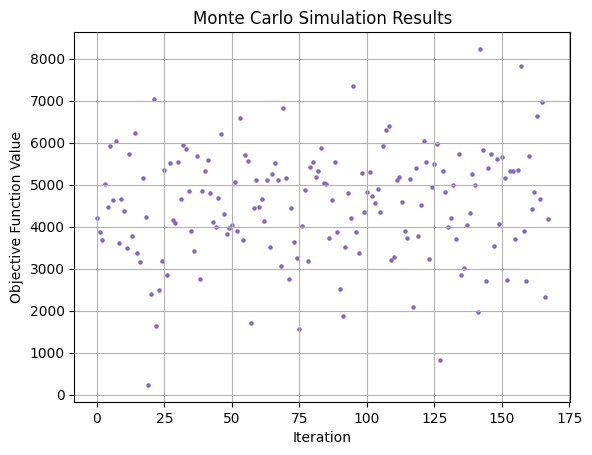
\includegraphics[width=327.75pt,height=251.9pt]{latexImage_bc888168c10ea3a4ba51a6bfe0d3daa4.png}}
\end{picture}
\begin{tikzpicture}[overlay]
\path(0pt,0pt);
\filldraw[color_283006][even odd rule]
(55.9pt, -332.561pt) -- (132.85pt, -332.561pt)
 -- (132.85pt, -332.561pt)
 -- (132.85pt, -319.811pt)
 -- (132.85pt, -319.811pt)
 -- (55.9pt, -319.811pt) -- cycle
;
\end{tikzpicture}
\begin{picture}(-5,0)(2.5,0)
\put(56,-330.011){\fontsize{11}{1}\usefont{T1}{cmr}{m}{n}\selectfont\color{color_80434}对成本效益比率}
\end{picture}
\begin{tikzpicture}[overlay]
\path(0pt,0pt);
\filldraw[color_283006][even odd rule]
(180.2pt, -332.561pt) -- (312.15pt, -332.561pt)
 -- (312.15pt, -332.561pt)
 -- (312.15pt, -319.811pt)
 -- (312.15pt, -319.811pt)
 -- (180.2pt, -319.811pt) -- cycle
;
\end{tikzpicture}
\begin{picture}(-5,0)(2.5,0)
\put(180.3,-330.011){\fontsize{11}{1}\usefont{T1}{cmr}{m}{n}\selectfont\color{color_80434},}
\put(191.3,-330.011){\fontsize{11}{1}\usefont{T1}{cmr}{m}{n}\selectfont\color{color_80434}我}
\put(202.3,-330.011){\fontsize{11}{1}\usefont{T1}{cmr}{m}{n}\selectfont\color{color_80434}们首先要确定}
\put(268.3,-330.011){\fontsize{11}{1}\usefont{T1}{cmr}{m}{n}\selectfont\color{color_80434}每}
\put(279.3,-330.011){\fontsize{11}{1}\usefont{T1}{cmr}{m}{n}\selectfont\color{color_80434}个变}
\put(301.3,-330.011){\fontsize{11}{1}\usefont{T1}{cmr}{m}{n}\selectfont\color{color_80434}量}
\end{picture}
\begin{tikzpicture}[overlay]
\path(0pt,0pt);
\filldraw[color_283006][even odd rule]
(373.7pt, -332.561pt) -- (505.65pt, -332.561pt)
 -- (505.65pt, -332.561pt)
 -- (505.65pt, -319.811pt)
 -- (505.65pt, -319.811pt)
 -- (373.7pt, -319.811pt) -- cycle
;
\end{tikzpicture}
\begin{picture}(-5,0)(2.5,0)
\put(373.8,-330.011){\fontsize{11}{1}\usefont{T1}{cmr}{m}{n}\selectfont\color{color_80434}的概率分布,根据概率分布}
\end{picture}
\begin{tikzpicture}[overlay]
\path(0pt,0pt);
\filldraw[color_283006][even odd rule]
(55.9pt, -345.361pt) -- (506.85pt, -345.361pt)
 -- (506.85pt, -345.361pt)
 -- (506.85pt, -332.611pt)
 -- (506.85pt, -332.611pt)
 -- (55.9pt, -332.611pt) -- cycle
;
\end{tikzpicture}
\begin{picture}(-5,0)(2.5,0)
\put(56,-342.811){\fontsize{11}{1}\usefont{T1}{cmr}{m}{n}\selectfont\color{color_80434}生}
\put(67,-342.811){\fontsize{11}{1}\usefont{T1}{cmr}{m}{n}\selectfont\color{color_80434}成}
\put(78,-342.811){\fontsize{11}{1}\usefont{T1}{cmr}{m}{n}\selectfont\color{color_80434}大量}
\put(100,-342.811){\fontsize{11}{1}\usefont{T1}{cmr}{m}{n}\selectfont\color{color_80434}随机}
\put(122,-342.811){\fontsize{11}{1}\usefont{T1}{cmr}{m}{n}\selectfont\color{color_80434}样}
\put(133,-342.811){\fontsize{11}{1}\usefont{T1}{cmr}{m}{n}\selectfont\color{color_80434}本,}
\put(155,-342.811){\fontsize{11}{1}\usefont{T1}{cmr}{m}{n}\selectfont\color{color_80434}再}
\put(166,-342.811){\fontsize{11}{1}\usefont{T1}{cmr}{m}{n}\selectfont\color{color_80434}计算相对应的目标函数}
\put(276,-342.811){\fontsize{11}{1}\usefont{T1}{cmr}{m}{n}\selectfont\color{color_80434}值}
\put(287,-342.811){\fontsize{11}{1}\usefont{T1}{cmr}{m}{n}\selectfont\color{color_80434},收集}
\put(320,-342.811){\fontsize{11}{1}\usefont{T1}{cmr}{m}{n}\selectfont\color{color_80434}所}
\put(331,-342.811){\fontsize{11}{1}\usefont{T1}{cmr}{m}{n}\selectfont\color{color_80434}有的目标函数}
\put(397,-342.811){\fontsize{11}{1}\usefont{T1}{cmr}{m}{n}\selectfont\color{color_80434}值}
\put(408,-342.811){\fontsize{11}{1}\usefont{T1}{cmr}{m}{n}\selectfont\color{color_80434},进行}
\put(441,-342.811){\fontsize{11}{1}\usefont{T1}{cmr}{m}{n}\selectfont\color{color_80434}统}
\put(452,-342.811){\fontsize{11}{1}\usefont{T1}{cmr}{m}{n}\selectfont\color{color_80434}计分析,计}
\end{picture}
\begin{tikzpicture}[overlay]
\path(0pt,0pt);
\filldraw[color_283006][even odd rule]
(55.9pt, -358.161pt) -- (220.85pt, -358.161pt)
 -- (220.85pt, -358.161pt)
 -- (220.85pt, -345.411pt)
 -- (220.85pt, -345.411pt)
 -- (55.9pt, -345.411pt) -- cycle
;
\end{tikzpicture}
\begin{picture}(-5,0)(2.5,0)
\put(56,-355.611){\fontsize{11}{1}\usefont{T1}{cmr}{m}{n}\selectfont\color{color_80434}算出}
\put(78,-355.611){\fontsize{11}{1}\usefont{T1}{cmr}{m}{n}\selectfont\color{color_80434}均值}
\put(100,-355.611){\fontsize{11}{1}\usefont{T1}{cmr}{m}{n}\selectfont\color{color_80434}和方}
\put(122,-355.611){\fontsize{11}{1}\usefont{T1}{cmr}{m}{n}\selectfont\color{color_80434}差}
\put(133,-355.611){\fontsize{11}{1}\usefont{T1}{cmr}{m}{n}\selectfont\color{color_80434},}
\put(144,-355.611){\fontsize{11}{1}\usefont{T1}{cmr}{m}{n}\selectfont\color{color_80434}经}
\put(155,-355.611){\fontsize{11}{1}\usefont{T1}{cmr}{m}{n}\selectfont\color{color_80434}过}
\put(166,-355.611){\fontsize{11}{1}\usefont{T1}{cmr}{m}{n}\selectfont\color{color_80434}处}
\put(177,-355.611){\fontsize{11}{1}\usefont{T1}{cmr}{m}{n}\selectfont\color{color_80434}理得到:}
\end{picture}
\begin{tikzpicture}[overlay]
\path(0pt,0pt);
\filldraw[color_283006][even odd rule]
(179pt, -373.861pt) -- (386.35pt, -373.861pt)
 -- (386.35pt, -373.861pt)
 -- (386.35pt, -361.211pt)
 -- (386.35pt, -361.211pt)
 -- (179pt, -361.211pt) -- cycle
;
\end{tikzpicture}
\begin{picture}(-5,0)(2.5,0)
\put(179.1,-371.511){\fontsize{11}{1}\usefont{T1}{ptm}{m}{n}\selectfont\color{color_80434}M}
\put(188.802,-371.511){\fontsize{11}{1}\usefont{T1}{ptm}{m}{n}\selectfont\color{color_80434}e}
\put(193.686,-371.511){\fontsize{11}{1}\usefont{T1}{ptm}{m}{n}\selectfont\color{color_80434}a}
\put(198.57,-371.511){\fontsize{11}{1}\usefont{T1}{ptm}{m}{n}\selectfont\color{color_80434}n }
\put(206.864,-371.511){\fontsize{11}{1}\usefont{T1}{ptm}{m}{n}\selectfont\color{color_80434}va}
\put(217.16,-371.511){\fontsize{11}{1}\usefont{T1}{ptm}{m}{n}\selectfont\color{color_80434}l}
\put(220.251,-371.511){\fontsize{11}{1}\usefont{T1}{ptm}{m}{n}\selectfont\color{color_80434}ue}
\put(230.635,-371.511){\fontsize{11}{1}\usefont{T1}{ptm}{m}{n}\selectfont\color{color_80434} }
\put(233.429,-371.511){\fontsize{11}{1}\usefont{T1}{ptm}{m}{n}\selectfont\color{color_80434}o}
\put(238.83,-371.511){\fontsize{11}{1}\usefont{T1}{ptm}{m}{n}\selectfont\color{color_80434}f}
\put(242.515,-371.511){\fontsize{11}{1}\usefont{T1}{ptm}{m}{n}\selectfont\color{color_80434} }
\put(245.3091,-371.511){\fontsize{11}{1}\usefont{T1}{ptm}{m}{n}\selectfont\color{color_80434}C}
\put(252.613,-371.511){\fontsize{11}{1}\usefont{T1}{ptm}{m}{n}\selectfont\color{color_80434}E}
\put(259.312,-371.511){\fontsize{11}{1}\usefont{T1}{ptm}{m}{n}\selectfont\color{color_80434}R}
\put(266.616,-371.511){\fontsize{11}{1}\usefont{T1}{ptm}{m}{n}\selectfont\color{color_80434}(}
\put(270.301,-371.511){\fontsize{11}{1}\usefont{T1}{ptm}{m}{n}\selectfont\color{color_80434}e}
\put(275.185,-371.511){\fontsize{11}{1}\usefont{T1}{ptm}{m}{n}\selectfont\color{color_80434})}
\put(278.782,-371.511){\fontsize{11}{1}\usefont{T1}{ptm}{m}{n}\selectfont\color{color_80434}:}
\put(281.873,-371.511){\fontsize{11}{1}\usefont{T1}{ptm}{m}{n}\selectfont\color{color_80434} }
\put(284.667,-371.511){\fontsize{11}{1}\usefont{T1}{ptm}{m}{n}\selectfont\color{color_80434}0}
\put(290.068,-371.511){\fontsize{11}{1}\usefont{T1}{ptm}{m}{n}\selectfont\color{color_80434}.}
\put(292.862,-371.511){\fontsize{11}{1}\usefont{T1}{ptm}{m}{n}\selectfont\color{color_80434}07217944998576989}
\end{picture}
\begin{tikzpicture}[overlay]
\path(0pt,0pt);
\filldraw[color_283006][even odd rule]
(157.9pt, -389.461pt) -- (407.45pt, -389.461pt)
 -- (407.45pt, -389.461pt)
 -- (407.45pt, -376.911pt)
 -- (407.45pt, -376.911pt)
 -- (157.9pt, -376.911pt) -- cycle
;
\end{tikzpicture}
\begin{picture}(-5,0)(2.5,0)
\put(158,-387.111){\fontsize{11}{1}\usefont{T1}{ptm}{m}{n}\selectfont\color{color_80434}S}
\put(164.105,-387.111){\fontsize{11}{1}\usefont{T1}{ptm}{m}{n}\selectfont\color{color_80434}t}
\put(167.108,-387.111){\fontsize{11}{1}\usefont{T1}{ptm}{m}{n}\selectfont\color{color_80434}a}
\put(171.992,-387.111){\fontsize{11}{1}\usefont{T1}{ptm}{m}{n}\selectfont\color{color_80434}nda}
\put(187.876,-387.111){\fontsize{11}{1}\usefont{T1}{ptm}{m}{n}\selectfont\color{color_80434}r}
\put(191.561,-387.111){\fontsize{11}{1}\usefont{T1}{ptm}{m}{n}\selectfont\color{color_80434}d }
\put(199.756,-387.111){\fontsize{11}{1}\usefont{T1}{ptm}{m}{n}\selectfont\color{color_80434}de}
\put(210.14,-387.111){\fontsize{11}{1}\usefont{T1}{ptm}{m}{n}\selectfont\color{color_80434}vi}
\put(218.731,-387.111){\fontsize{11}{1}\usefont{T1}{ptm}{m}{n}\selectfont\color{color_80434}a}
\put(223.527,-387.111){\fontsize{11}{1}\usefont{T1}{ptm}{m}{n}\selectfont\color{color_80434}t}
\put(226.618,-387.111){\fontsize{11}{1}\usefont{T1}{ptm}{m}{n}\selectfont\color{color_80434}i}
\put(229.709,-387.111){\fontsize{11}{1}\usefont{T1}{ptm}{m}{n}\selectfont\color{color_80434}on }
\put(243.404,-387.111){\fontsize{11}{1}\usefont{T1}{ptm}{m}{n}\selectfont\color{color_80434}of}
\put(252.589,-387.111){\fontsize{11}{1}\usefont{T1}{ptm}{m}{n}\selectfont\color{color_80434} }
\put(255.284,-387.111){\fontsize{11}{1}\usefont{T1}{ptm}{m}{n}\selectfont\color{color_80434}C}
\put(262.588,-387.111){\fontsize{11}{1}\usefont{T1}{ptm}{m}{n}\selectfont\color{color_80434}E}
\put(269.375,-387.111){\fontsize{11}{1}\usefont{T1}{ptm}{m}{n}\selectfont\color{color_80434}R}
\put(276.679,-387.111){\fontsize{11}{1}\usefont{T1}{ptm}{m}{n}\selectfont\color{color_80434}(}
\put(280.364,-387.111){\fontsize{11}{1}\usefont{T1}{ptm}{m}{n}\selectfont\color{color_80434}e}
\put(285.16,-387.111){\fontsize{11}{1}\usefont{T1}{ptm}{m}{n}\selectfont\color{color_80434})}
\put(288.845,-387.111){\fontsize{11}{1}\usefont{T1}{ptm}{m}{n}\selectfont\color{color_80434}:}
\put(291.936,-387.111){\fontsize{11}{1}\usefont{T1}{ptm}{m}{n}\selectfont\color{color_80434} }
\put(294.73,-387.111){\fontsize{11}{1}\usefont{T1}{ptm}{m}{n}\selectfont\color{color_80434}0}
\put(300.131,-387.111){\fontsize{11}{1}\usefont{T1}{ptm}{m}{n}\selectfont\color{color_80434}.}
\put(302.925,-387.111){\fontsize{11}{1}\usefont{T1}{ptm}{m}{n}\selectfont\color{color_80434}0036991256889698423}
\put(78,-423.111){\fontsize{16}{1}\usefont{T1}{ptm}{b}{n}\selectfont\color{color_55609}5}
\put(86,-423.111){\fontsize{16}{1}\usefont{T1}{cmr}{m}{n}\selectfont\color{color_55609}、}
\put(119,-423.111){\fontsize{16}{1}\usefont{T1}{cmr}{m}{n}\selectfont\color{color_55609}额外的设备}
\put(199,-423.111){\fontsize{16}{1}\usefont{T1}{ptm}{b}{n}\selectfont\color{color_55609} }
\put(204.504,-423.111){\fontsize{16}{1}\usefont{T1}{ptm}{b}{n}\selectfont\color{color_55609} }
\put(56,-453.111){\fontsize{14}{1}\usefont{T1}{ptm}{b}{n}\selectfont\color{color_55609}a}
\put(62.902,-453.111){\fontsize{14}{1}\usefont{T1}{ptm}{b}{n}\selectfont\color{color_55609})}
\put(67.592,-453.111){\fontsize{14}{1}\usefont{T1}{ptm}{b}{n}\selectfont\color{color_55609} }
\put(71.1,-453.111){\fontsize{14}{1}\usefont{T1}{cmr}{m}{n}\selectfont\color{color_55609}急}
\put(85.1,-453.111){\fontsize{14}{1}\usefont{T1}{cmr}{m}{n}\selectfont\color{color_55609}求}
\put(99.1,-453.111){\fontsize{14}{1}\usefont{T1}{cmr}{m}{n}\selectfont\color{color_55609}设备}
\put(56,-481.111){\fontsize{11}{1}\usefont{T1}{cmr}{m}{n}\selectfont\color{color_80434}}
\put(72.8,-481.111){\fontsize{11}{1}\usefont{T1}{cmr}{m}{n}\selectfont\color{color_80434}紧急呼吸}
\put(116.8,-481.111){\fontsize{11}{1}\usefont{T1}{cmr}{m}{n}\selectfont\color{color_80434}设备(}
\put(149.8,-481.111){\fontsize{11}{1}\usefont{T1}{ptm}{m}{n}\selectfont\color{color_80434}E}
\put(156.499,-481.111){\fontsize{11}{1}\usefont{T1}{ptm}{m}{n}\selectfont\color{color_80434}B}
\put(163.803,-481.111){\fontsize{11}{1}\usefont{T1}{ptm}{m}{n}\selectfont\color{color_80434}A}
\put(171.701,-481.111){\fontsize{11}{1}\usefont{T1}{ptm}{m}{n}\selectfont\color{color_80434}s}
\put(176.1,-481.111){\fontsize{11}{1}\usefont{T1}{cmr}{m}{n}\selectfont\color{color_80434}):用于}
\put(220.1,-481.111){\fontsize{11}{1}\usefont{T1}{cmr}{m}{n}\selectfont\color{color_80434}紧急}
\put(242.1,-481.111){\fontsize{11}{1}\usefont{T1}{cmr}{m}{n}\selectfont\color{color_80434}救}
\put(253.1,-481.111){\fontsize{11}{1}\usefont{T1}{cmr}{m}{n}\selectfont\color{color_80434}治伤者}
\put(286.1,-481.111){\fontsize{11}{1}\usefont{T1}{cmr}{m}{n}\selectfont\color{color_80434},}
\put(297.1,-481.111){\fontsize{11}{1}\usefont{T1}{cmr}{m}{n}\selectfont\color{color_80434}挽}
\put(308.1,-481.111){\fontsize{11}{1}\usefont{T1}{cmr}{m}{n}\selectfont\color{color_80434}救}
\put(319.1,-481.111){\fontsize{11}{1}\usefont{T1}{cmr}{m}{n}\selectfont\color{color_80434}伤者}
\put(341.1,-481.111){\fontsize{11}{1}\usefont{T1}{cmr}{m}{n}\selectfont\color{color_80434}生命}
\put(56,-499.811){\fontsize{14}{1}\usefont{T1}{ptm}{b}{n}\selectfont\color{color_55609}b}
\put(63.8,-499.811){\fontsize{14}{1}\usefont{T1}{cmr}{m}{n}\selectfont\color{color_55609})}
\put(77.8,-499.811){\fontsize{14}{1}\usefont{T1}{cmr}{m}{n}\selectfont\color{color_55609}深}
\put(91.8,-499.811){\fontsize{14}{1}\usefont{T1}{cmr}{m}{n}\selectfont\color{color_55609}海设备}
\put(56,-527.811){\fontsize{11}{1}\usefont{T1}{cmr}{m}{n}\selectfont\color{color_80434}}
\put(72.8,-527.811){\fontsize{11}{1}\usefont{T1}{ptm}{m}{n}\selectfont\color{color_80434}D}
\put(80.69801,-527.811){\fontsize{11}{1}\usefont{T1}{ptm}{m}{n}\selectfont\color{color_80434}e}
\put(85.58201,-527.811){\fontsize{11}{1}\usefont{T1}{ptm}{m}{n}\selectfont\color{color_80434}e}
\put(90.46601,-527.811){\fontsize{11}{1}\usefont{T1}{ptm}{m}{n}\selectfont\color{color_80434}p-}
\put(99.65101,-527.811){\fontsize{11}{1}\usefont{T1}{ptm}{m}{n}\selectfont\color{color_80434}s}
\put(103.853,-527.811){\fontsize{11}{1}\usefont{T1}{ptm}{m}{n}\selectfont\color{color_80434}e}
\put(108.737,-527.811){\fontsize{11}{1}\usefont{T1}{ptm}{m}{n}\selectfont\color{color_80434}a}
\put(113.621,-527.811){\fontsize{11}{1}\usefont{T1}{ptm}{m}{n}\selectfont\color{color_80434} }
\put(116.415,-527.811){\fontsize{11}{1}\usefont{T1}{ptm}{m}{n}\selectfont\color{color_80434}C}
\put(123.719,-527.811){\fontsize{11}{1}\usefont{T1}{ptm}{m}{n}\selectfont\color{color_80434}a}
\put(128.515,-527.811){\fontsize{11}{1}\usefont{T1}{ptm}{m}{n}\selectfont\color{color_80434}m}
\put(137.106,-527.811){\fontsize{11}{1}\usefont{T1}{ptm}{m}{n}\selectfont\color{color_80434}e}
\put(141.99,-527.811){\fontsize{11}{1}\usefont{T1}{ptm}{m}{n}\selectfont\color{color_80434}r}
\put(145.675,-527.811){\fontsize{11}{1}\usefont{T1}{ptm}{m}{n}\selectfont\color{color_80434}a}
\put(150.471,-527.811){\fontsize{11}{1}\usefont{T1}{ptm}{m}{n}\selectfont\color{color_80434}:}
\put(153.7,-527.811){\fontsize{11}{1}\usefont{T1}{cmr}{m}{n}\selectfont\color{color_80434}使用可以}
\put(197.7,-527.811){\fontsize{11}{1}\usefont{T1}{cmr}{m}{n}\selectfont\color{color_80434}承}
\put(208.7,-527.811){\fontsize{11}{1}\usefont{T1}{cmr}{m}{n}\selectfont\color{color_80434}受高水}
\put(241.7,-527.811){\fontsize{11}{1}\usefont{T1}{cmr}{m}{n}\selectfont\color{color_80434}压}
\put(252.7,-527.811){\fontsize{11}{1}\usefont{T1}{cmr}{m}{n}\selectfont\color{color_80434}的}
\put(263.7,-527.811){\fontsize{11}{1}\usefont{T1}{cmr}{m}{n}\selectfont\color{color_80434}摄像}
\put(285.7,-527.811){\fontsize{11}{1}\usefont{T1}{cmr}{m}{n}\selectfont\color{color_80434}机,可以在}
\put(340.7,-527.811){\fontsize{11}{1}\usefont{T1}{cmr}{m}{n}\selectfont\color{color_80434}深}
\put(351.7,-527.811){\fontsize{11}{1}\usefont{T1}{cmr}{m}{n}\selectfont\color{color_80434}海中}
\put(373.7,-527.811){\fontsize{11}{1}\usefont{T1}{cmr}{m}{n}\selectfont\color{color_80434}捕捉}
\put(395.7,-527.811){\fontsize{11}{1}\usefont{T1}{cmr}{m}{n}\selectfont\color{color_80434}图}
\put(406.7,-527.811){\fontsize{11}{1}\usefont{T1}{cmr}{m}{n}\selectfont\color{color_80434}像}
\put(417.7,-527.811){\fontsize{11}{1}\usefont{T1}{cmr}{m}{n}\selectfont\color{color_80434},}
\put(428.7,-527.811){\fontsize{11}{1}\usefont{T1}{cmr}{m}{n}\selectfont\color{color_80434}帮助}
\put(450.7,-527.811){\fontsize{11}{1}\usefont{T1}{cmr}{m}{n}\selectfont\color{color_80434}定位潜水器}
\put(56,-543.711){\fontsize{11}{1}\usefont{T1}{cmr}{m}{n}\selectfont\color{color_80434}}
\put(72.8,-543.711){\fontsize{11}{1}\usefont{T1}{cmr}{m}{n}\selectfont\color{color_80434}惯}
\put(83.8,-543.711){\fontsize{11}{1}\usefont{T1}{cmr}{m}{n}\selectfont\color{color_80434}性}
\put(94.8,-543.711){\fontsize{11}{1}\usefont{T1}{cmr}{m}{n}\selectfont\color{color_80434}导航}
\put(116.8,-543.711){\fontsize{11}{1}\usefont{T1}{cmr}{m}{n}\selectfont\color{color_80434}系}
\put(127.8,-543.711){\fontsize{11}{1}\usefont{T1}{cmr}{m}{n}\selectfont\color{color_80434}统}
\put(138.8,-543.711){\fontsize{11}{1}\usefont{T1}{cmr}{m}{n}\selectfont\color{color_80434}(}
\put(149.8,-543.711){\fontsize{11}{1}\usefont{T1}{ptm}{m}{n}\selectfont\color{color_80434}I}
\put(153.485,-543.711){\fontsize{11}{1}\usefont{T1}{ptm}{m}{n}\selectfont\color{color_80434}N}
\put(161.383,-543.711){\fontsize{11}{1}\usefont{T1}{ptm}{m}{n}\selectfont\color{color_80434}S}
\put(167.5,-543.711){\fontsize{11}{1}\usefont{T1}{cmr}{m}{n}\selectfont\color{color_80434}):}
\put(189.5,-543.711){\fontsize{11}{1}\usefont{T1}{cmr}{m}{n}\selectfont\color{color_80434}惯}
\put(200.5,-543.711){\fontsize{11}{1}\usefont{T1}{cmr}{m}{n}\selectfont\color{color_80434}性}
\put(211.5,-543.711){\fontsize{11}{1}\usefont{T1}{cmr}{m}{n}\selectfont\color{color_80434}导航}
\put(233.5,-543.711){\fontsize{11}{1}\usefont{T1}{cmr}{m}{n}\selectfont\color{color_80434}系}
\put(244.5,-543.711){\fontsize{11}{1}\usefont{T1}{cmr}{m}{n}\selectfont\color{color_80434}统}
\put(255.5,-543.711){\fontsize{11}{1}\usefont{T1}{cmr}{m}{n}\selectfont\color{color_80434}利}
\put(266.5,-543.711){\fontsize{11}{1}\usefont{T1}{cmr}{m}{n}\selectfont\color{color_80434}用加}
\put(288.5,-543.711){\fontsize{11}{1}\usefont{T1}{cmr}{m}{n}\selectfont\color{color_80434}速度}
\put(310.5,-543.711){\fontsize{11}{1}\usefont{T1}{cmr}{m}{n}\selectfont\color{color_80434}计和}
\put(332.5,-543.711){\fontsize{11}{1}\usefont{T1}{cmr}{m}{n}\selectfont\color{color_80434}陀螺仪}
\put(365.5,-543.711){\fontsize{11}{1}\usefont{T1}{cmr}{m}{n}\selectfont\color{color_80434}来}
\put(376.5,-543.711){\fontsize{11}{1}\usefont{T1}{cmr}{m}{n}\selectfont\color{color_80434}测}
\put(387.5,-543.711){\fontsize{11}{1}\usefont{T1}{cmr}{m}{n}\selectfont\color{color_80434}量}
\put(398.5,-543.711){\fontsize{11}{1}\usefont{T1}{cmr}{m}{n}\selectfont\color{color_80434}和计算潜水器的位置、}
\put(72.8,-556.511){\fontsize{11}{1}\usefont{T1}{cmr}{m}{n}\selectfont\color{color_80434}速度}
\put(94.8,-556.511){\fontsize{11}{1}\usefont{T1}{cmr}{m}{n}\selectfont\color{color_80434}、方向等动态参数}
\put(182.8,-556.511){\fontsize{11}{1}\usefont{T1}{ptm}{m}{n}\selectfont\color{color_80434};}
\put(185.8,-556.511){\fontsize{11}{1}\usefont{T1}{cmr}{m}{n}\selectfont\color{color_80434}它不}
\put(207.8,-556.511){\fontsize{11}{1}\usefont{T1}{cmr}{m}{n}\selectfont\color{color_80434}依赖}
\put(229.8,-556.511){\fontsize{11}{1}\usefont{T1}{cmr}{m}{n}\selectfont\color{color_80434}于外部信}
\put(273.8,-556.511){\fontsize{11}{1}\usefont{T1}{cmr}{m}{n}\selectfont\color{color_80434}号}
\put(284.8,-556.511){\fontsize{11}{1}\usefont{T1}{cmr}{m}{n}\selectfont\color{color_80434},因此在水下环境中}
\put(383.8,-556.511){\fontsize{11}{1}\usefont{T1}{cmr}{m}{n}\selectfont\color{color_80434}非}
\put(394.8,-556.511){\fontsize{11}{1}\usefont{T1}{cmr}{m}{n}\selectfont\color{color_80434}常}
\put(405.8,-556.511){\fontsize{11}{1}\usefont{T1}{cmr}{m}{n}\selectfont\color{color_80434}适}
\put(416.8,-556.511){\fontsize{11}{1}\usefont{T1}{cmr}{m}{n}\selectfont\color{color_80434}用}
\put(56,-575.211){\fontsize{14}{1}\usefont{T1}{ptm}{b}{n}\selectfont\color{color_55609}c)}
\put(66.892,-575.211){\fontsize{14}{1}\usefont{T1}{ptm}{b}{n}\selectfont\color{color_55609} }
\put(70.4,-575.211){\fontsize{14}{1}\usefont{T1}{cmr}{m}{n}\selectfont\color{color_55609}浅}
\put(84.4,-575.211){\fontsize{14}{1}\usefont{T1}{cmr}{m}{n}\selectfont\color{color_55609}水区域}
\put(126.4,-575.211){\fontsize{14}{1}\usefont{T1}{cmr}{m}{n}\selectfont\color{color_55609}或}
\put(140.4,-575.211){\fontsize{14}{1}\usefont{T1}{cmr}{m}{n}\selectfont\color{color_55609}水面设备}
\put(56,-603.211){\fontsize{11}{1}\usefont{T1}{cmr}{m}{n}\selectfont\color{color_80434}}
\put(72.8,-603.211){\fontsize{11}{1}\usefont{T1}{cmr}{m}{n}\selectfont\color{color_80434}卫星}
\put(94.8,-603.211){\fontsize{11}{1}\usefont{T1}{cmr}{m}{n}\selectfont\color{color_80434}定位系}
\put(127.8,-603.211){\fontsize{11}{1}\usefont{T1}{cmr}{m}{n}\selectfont\color{color_80434}统}
\put(138.8,-603.211){\fontsize{11}{1}\usefont{T1}{cmr}{m}{n}\selectfont\color{color_80434}(如}
\put(163,-603.211){\fontsize{11}{1}\usefont{T1}{ptm}{m}{n}\selectfont\color{color_80434}G}
\put(170.898,-603.211){\fontsize{11}{1}\usefont{T1}{ptm}{m}{n}\selectfont\color{color_80434}P}
\put(177.003,-603.211){\fontsize{11}{1}\usefont{T1}{ptm}{m}{n}\selectfont\color{color_80434}S}
\put(185.4,-603.211){\fontsize{11}{1}\usefont{T1}{cmr}{m}{n}\selectfont\color{color_80434}接}
\put(196.4,-603.211){\fontsize{11}{1}\usefont{T1}{cmr}{m}{n}\selectfont\color{color_80434}收机):}
\put(240.4,-603.211){\fontsize{11}{1}\usefont{T1}{cmr}{m}{n}\selectfont\color{color_80434}虽然}
\put(264.6,-603.211){\fontsize{11}{1}\usefont{T1}{ptm}{m}{n}\selectfont\color{color_80434}G}
\put(272.498,-603.211){\fontsize{11}{1}\usefont{T1}{ptm}{m}{n}\selectfont\color{color_80434}P}
\put(278.603,-603.211){\fontsize{11}{1}\usefont{T1}{ptm}{m}{n}\selectfont\color{color_80434}S}
\put(287,-603.211){\fontsize{11}{1}\usefont{T1}{cmr}{m}{n}\selectfont\color{color_80434}信}
\put(298,-603.211){\fontsize{11}{1}\usefont{T1}{cmr}{m}{n}\selectfont\color{color_80434}号无}
\put(320,-603.211){\fontsize{11}{1}\usefont{T1}{cmr}{m}{n}\selectfont\color{color_80434}法}
\put(331,-603.211){\fontsize{11}{1}\usefont{T1}{cmr}{m}{n}\selectfont\color{color_80434}直接}
\put(353,-603.211){\fontsize{11}{1}\usefont{T1}{cmr}{m}{n}\selectfont\color{color_80434}在水下使用,}
\put(419,-603.211){\fontsize{11}{1}\usefont{T1}{cmr}{m}{n}\selectfont\color{color_80434}但}
\put(430,-603.211){\fontsize{11}{1}\usefont{T1}{cmr}{m}{n}\selectfont\color{color_80434}潜水器在}
\put(474,-603.211){\fontsize{11}{1}\usefont{T1}{cmr}{m}{n}\selectfont\color{color_80434}浮}
\put(485,-603.211){\fontsize{11}{1}\usefont{T1}{cmr}{m}{n}\selectfont\color{color_80434}出水}
\put(72.8,-616.111){\fontsize{11}{1}\usefont{T1}{cmr}{m}{n}\selectfont\color{color_80434}面时可以}
\put(116.8,-616.111){\fontsize{11}{1}\usefont{T1}{cmr}{m}{n}\selectfont\color{color_80434}利}
\put(127.8,-616.111){\fontsize{11}{1}\usefont{T1}{cmr}{m}{n}\selectfont\color{color_80434}用}
\put(141,-616.111){\fontsize{11}{1}\usefont{T1}{ptm}{m}{n}\selectfont\color{color_80434}G}
\put(148.898,-616.111){\fontsize{11}{1}\usefont{T1}{ptm}{m}{n}\selectfont\color{color_80434}P}
\put(155.003,-616.111){\fontsize{11}{1}\usefont{T1}{ptm}{m}{n}\selectfont\color{color_80434}S}
\put(163.4,-616.111){\fontsize{11}{1}\usefont{T1}{cmr}{m}{n}\selectfont\color{color_80434}进行}
\put(185.4,-616.111){\fontsize{11}{1}\usefont{T1}{cmr}{m}{n}\selectfont\color{color_80434}精}
\put(196.4,-616.111){\fontsize{11}{1}\usefont{T1}{cmr}{m}{n}\selectfont\color{color_80434}确定位}
\put(229.4,-616.111){\fontsize{11}{1}\usefont{T1}{ptm}{m}{n}\selectfont\color{color_80434},}
\put(232.1,-616.111){\fontsize{11}{1}\usefont{T1}{cmr}{m}{n}\selectfont\color{color_80434}这些数据可以用}
\put(309.1,-616.111){\fontsize{11}{1}\usefont{T1}{cmr}{m}{n}\selectfont\color{color_80434}来}
\put(320.1,-616.111){\fontsize{11}{1}\usefont{T1}{cmr}{m}{n}\selectfont\color{color_80434}校}
\put(331.1,-616.111){\fontsize{11}{1}\usefont{T1}{cmr}{m}{n}\selectfont\color{color_80434}准和验证}
\put(375.1,-616.111){\fontsize{11}{1}\usefont{T1}{cmr}{m}{n}\selectfont\color{color_80434}其他导航}
\put(419.1,-616.111){\fontsize{11}{1}\usefont{T1}{cmr}{m}{n}\selectfont\color{color_80434}系}
\put(430.1,-616.111){\fontsize{11}{1}\usefont{T1}{cmr}{m}{n}\selectfont\color{color_80434}统}
\put(441.1,-616.111){\fontsize{11}{1}\usefont{T1}{cmr}{m}{n}\selectfont\color{color_80434}的准确性}
\put(56,-638.411){\fontsize{18}{1}\usefont{T1}{cmr}{m}{n}\selectfont\color{color_55609}六}
\put(74,-638.411){\fontsize{18}{1}\usefont{T1}{cmr}{m}{n}\selectfont\color{color_55609}、}
\put(98,-638.411){\fontsize{18}{1}\usefont{T1}{cmr}{m}{n}\selectfont\color{color_55609}模拟搜索}
\put(78,-672.211){\fontsize{16}{1}\usefont{T1}{ptm}{b}{n}\selectfont\color{color_55609}1}
\put(86,-672.211){\fontsize{16}{1}\usefont{T1}{cmr}{m}{n}\selectfont\color{color_55609}、}
\put(119,-672.211){\fontsize{16}{1}\usefont{T1}{cmr}{m}{n}\selectfont\color{color_55609}问题分析}
\put(56,-703.311){\fontsize{12}{1}\usefont{T1}{cmr}{m}{n}\selectfont\color{color_80434}我}
\put(68,-703.311){\fontsize{12}{1}\usefont{T1}{cmr}{m}{n}\selectfont\color{color_80434}们需要建立一个合}
\put(164,-703.311){\fontsize{12}{1}\usefont{T1}{cmr}{m}{n}\selectfont\color{color_80434}适}
\put(176,-703.311){\fontsize{12}{1}\usefont{T1}{cmr}{m}{n}\selectfont\color{color_80434}的模型}
\put(212,-703.311){\fontsize{12}{1}\usefont{T1}{cmr}{m}{n}\selectfont\color{color_80434}来}
\put(224,-703.311){\fontsize{12}{1}\usefont{T1}{cmr}{m}{n}\selectfont\color{color_80434}推荐设备的}
\put(284,-703.311){\fontsize{12}{1}\usefont{T1}{cmr}{m}{n}\selectfont\color{color_80434}初始}
\put(308,-703.311){\fontsize{12}{1}\usefont{T1}{cmr}{m}{n}\selectfont\color{color_80434}部署点和搜索模式,以}
\put(428,-703.311){\fontsize{12}{1}\usefont{T1}{cmr}{m}{n}\selectfont\color{color_80434}尽}
\put(440,-703.311){\fontsize{12}{1}\usefont{T1}{cmr}{m}{n}\selectfont\color{color_80434}量}
\put(452,-703.311){\fontsize{12}{1}\usefont{T1}{cmr}{m}{n}\selectfont\color{color_80434}减少}
\put(476,-703.311){\fontsize{12}{1}\usefont{T1}{cmr}{m}{n}\selectfont\color{color_80434}丢}
\put(488,-703.311){\fontsize{12}{1}\usefont{T1}{cmr}{m}{n}\selectfont\color{color_80434}失}
\put(56,-717.311){\fontsize{12}{1}\usefont{T1}{cmr}{m}{n}\selectfont\color{color_80434}潜水器的定位时间}
\put(152,-717.311){\fontsize{12}{1}\usefont{T1}{ptm}{m}{n}\selectfont\color{color_80434}.}
\end{picture}
\newpage
\begin{tikzpicture}[overlay]\path(0pt,0pt);\end{tikzpicture}
\begin{picture}(-5,0)(2.5,0)
\put(78,-76.51099){\fontsize{16}{1}\usefont{T1}{ptm}{b}{n}\selectfont\color{color_55609}2}
\put(86,-76.51099){\fontsize{16}{1}\usefont{T1}{cmr}{m}{n}\selectfont\color{color_55609}、}
\put(119,-76.51099){\fontsize{16}{1}\usefont{T1}{cmr}{m}{n}\selectfont\color{color_55609}模型的准备}
\put(100,-106.511){\fontsize{14}{1}\usefont{T1}{ptm}{b}{n}\selectfont\color{color_55609}a}
\put(106.902,-106.511){\fontsize{14}{1}\usefont{T1}{ptm}{b}{n}\selectfont\color{color_55609})}
\put(116.8,-106.511){\fontsize{14}{1}\usefont{T1}{cmr}{m}{n}\selectfont\color{color_55609}模型}
\put(144.8,-106.511){\fontsize{14}{1}\usefont{T1}{cmr}{m}{n}\selectfont\color{color_55609}假}
\put(158.8,-106.511){\fontsize{14}{1}\usefont{T1}{cmr}{m}{n}\selectfont\color{color_55609}设}
\put(56,-134.511){\fontsize{11}{1}\usefont{T1}{cmr}{m}{n}\selectfont\color{color_80434}}
\put(72.8,-134.511){\fontsize{11}{1}\usefont{T1}{cmr}{m}{n}\selectfont\color{color_80434}假}
\put(83.8,-134.511){\fontsize{11}{1}\usefont{T1}{cmr}{m}{n}\selectfont\color{color_80434}设搜索区域为预测}
\put(171.8,-134.511){\fontsize{11}{1}\usefont{T1}{cmr}{m}{n}\selectfont\color{color_80434}路}
\put(182.8,-134.511){\fontsize{11}{1}\usefont{T1}{cmr}{m}{n}\selectfont\color{color_80434}径}
\put(193.8,-134.511){\fontsize{11}{1}\usefont{T1}{cmr}{m}{n}\selectfont\color{color_80434}周}
\put(204.8,-134.511){\fontsize{11}{1}\usefont{T1}{cmr}{m}{n}\selectfont\color{color_80434}围}
\put(56,-150.311){\fontsize{11}{1}\usefont{T1}{cmr}{m}{n}\selectfont\color{color_80434}}
\put(72.8,-150.311){\fontsize{11}{1}\usefont{T1}{cmr}{m}{n}\selectfont\color{color_80434}假}
\put(83.8,-150.311){\fontsize{11}{1}\usefont{T1}{cmr}{m}{n}\selectfont\color{color_80434}设}
\put(97,-150.311){\fontsize{11}{1}\usefont{T1}{ptm}{m}{n}\selectfont\color{color_80434}10}
\put(107.901,-150.311){\fontsize{11}{1}\usefont{T1}{ptm}{m}{n}\selectfont\color{color_80434}m}
\put(116.492,-150.311){\fontsize{11}{1}\usefont{T1}{ptm}{m}{n}\selectfont\color{color_80434}i}
\put(119.583,-150.311){\fontsize{11}{1}\usefont{T1}{ptm}{m}{n}\selectfont\color{color_80434}n}
\put(127.3,-150.311){\fontsize{11}{1}\usefont{T1}{cmr}{m}{n}\selectfont\color{color_80434}未}
\put(138.3,-150.311){\fontsize{11}{1}\usefont{T1}{cmr}{m}{n}\selectfont\color{color_80434}收到潜艇发送的}
\put(215.3,-150.311){\fontsize{11}{1}\usefont{T1}{cmr}{m}{n}\selectfont\color{color_80434}消}
\put(226.3,-150.311){\fontsize{11}{1}\usefont{T1}{cmr}{m}{n}\selectfont\color{color_80434}息,}
\put(248.3,-150.311){\fontsize{11}{1}\usefont{T1}{cmr}{m}{n}\selectfont\color{color_80434}开始}
\put(270.3,-150.311){\fontsize{11}{1}\usefont{T1}{cmr}{m}{n}\selectfont\color{color_80434}搜索}
\put(56,-166.111){\fontsize{11}{1}\usefont{T1}{cmr}{m}{n}\selectfont\color{color_80434}}
\put(72.8,-166.111){\fontsize{11}{1}\usefont{T1}{cmr}{m}{n}\selectfont\color{color_80434}考虑}
\put(94.8,-166.111){\fontsize{11}{1}\usefont{T1}{cmr}{m}{n}\selectfont\color{color_80434}到潜水器定位}
\put(160.8,-166.111){\fontsize{11}{1}\usefont{T1}{cmr}{m}{n}\selectfont\color{color_80434}是}
\put(171.8,-166.111){\fontsize{11}{1}\usefont{T1}{cmr}{m}{n}\selectfont\color{color_80434}一个动态过程,模型可能需要定期更新以}
\put(369.8,-166.111){\fontsize{11}{1}\usefont{T1}{cmr}{m}{n}\selectfont\color{color_80434}适}
\put(380.8,-166.111){\fontsize{11}{1}\usefont{T1}{cmr}{m}{n}\selectfont\color{color_80434}应不}
\put(402.8,-166.111){\fontsize{11}{1}\usefont{T1}{cmr}{m}{n}\selectfont\color{color_80434}断}
\put(413.8,-166.111){\fontsize{11}{1}\usefont{T1}{cmr}{m}{n}\selectfont\color{color_80434}变化的环境和情况}
\put(100,-184.811){\fontsize{14}{1}\usefont{T1}{ptm}{b}{n}\selectfont\color{color_55609}b}
\put(107.7,-184.811){\fontsize{14}{1}\usefont{T1}{ptm}{b}{n}\selectfont\color{color_55609})}
\put(116.8,-184.811){\fontsize{14}{1}\usefont{T1}{cmr}{m}{n}\selectfont\color{color_55609}处}
\put(130.8,-184.811){\fontsize{14}{1}\usefont{T1}{cmr}{m}{n}\selectfont\color{color_55609}理}
\put(144.8,-184.811){\fontsize{14}{1}\usefont{T1}{cmr}{m}{n}\selectfont\color{color_55609}步}
\put(158.8,-184.811){\fontsize{14}{1}\usefont{T1}{cmr}{m}{n}\selectfont\color{color_55609}骤}
\put(56,-212.811){\fontsize{11}{1}\usefont{T1}{cmr}{m}{n}\selectfont\color{color_80434}}
\put(72.8,-212.811){\fontsize{11}{1}\usefont{T1}{cmr}{m}{n}\selectfont\color{color_80434}数据收集与预}
\put(138.8,-212.811){\fontsize{11}{1}\usefont{T1}{cmr}{m}{n}\selectfont\color{color_80434}处}
\put(149.8,-212.811){\fontsize{11}{1}\usefont{T1}{cmr}{m}{n}\selectfont\color{color_80434}理}
\put(56,-228.611){\fontsize{11}{1}\usefont{T1}{ptm}{m}{n}\selectfont\color{color_80434} }
\put(58.695,-228.611){\fontsize{11}{1}\usefont{T1}{ptm}{m}{n}\selectfont\color{color_80434} }
\put(61.489,-228.611){\fontsize{11}{1}\usefont{T1}{ptm}{m}{n}\selectfont\color{color_80434} }
\put(64.184,-228.611){\fontsize{11}{1}\usefont{T1}{ptm}{m}{n}\selectfont\color{color_80434} }
\put(66.978,-228.611){\fontsize{11}{1}\usefont{T1}{ptm}{m}{n}\selectfont\color{color_80434} }
\put(69.673,-228.611){\fontsize{11}{1}\usefont{T1}{ptm}{m}{n}\selectfont\color{color_80434} }
\put(72.5,-228.611){\fontsize{11}{1}\usefont{T1}{cmr}{m}{n}\selectfont\color{color_80434}我}
\put(83.5,-228.611){\fontsize{11}{1}\usefont{T1}{cmr}{m}{n}\selectfont\color{color_80434}们将随机}
\put(127.5,-228.611){\fontsize{11}{1}\usefont{T1}{cmr}{m}{n}\selectfont\color{color_80434}生}
\put(138.5,-228.611){\fontsize{11}{1}\usefont{T1}{cmr}{m}{n}\selectfont\color{color_80434}成潜水器与主船的}
\put(226.5,-228.611){\fontsize{11}{1}\usefont{T1}{cmr}{m}{n}\selectfont\color{color_80434}坐}
\put(237.5,-228.611){\fontsize{11}{1}\usefont{T1}{cmr}{m}{n}\selectfont\color{color_80434}标位置}
\put(270.5,-228.611){\fontsize{11}{1}\usefont{T1}{cmr}{m}{n}\selectfont\color{color_80434}保}
\put(281.5,-228.611){\fontsize{11}{1}\usefont{T1}{cmr}{m}{n}\selectfont\color{color_80434}存为数据集,}
\put(347.5,-228.611){\fontsize{11}{1}\usefont{T1}{cmr}{m}{n}\selectfont\color{color_80434}样}
\put(358.5,-228.611){\fontsize{11}{1}\usefont{T1}{cmr}{m}{n}\selectfont\color{color_80434}本}
\put(369.5,-228.611){\fontsize{11}{1}\usefont{T1}{cmr}{m}{n}\selectfont\color{color_80434}含}
\put(380.5,-228.611){\fontsize{11}{1}\usefont{T1}{cmr}{m}{n}\selectfont\color{color_80434}有}
\put(393.7,-228.611){\fontsize{11}{1}\usefont{T1}{ptm}{m}{n}\selectfont\color{color_80434}x}
\put(399.101,-228.611){\fontsize{11}{1}\usefont{T1}{ptm}{m}{n}\selectfont\color{color_80434},}
\put(401.895,-228.611){\fontsize{11}{1}\usefont{T1}{ptm}{m}{n}\selectfont\color{color_80434}y}
\put(406.592,-228.611){\fontsize{11}{1}\usefont{T1}{ptm}{m}{n}\selectfont\color{color_80434},}
\put(409.386,-228.611){\fontsize{11}{1}\usefont{T1}{ptm}{m}{n}\selectfont\color{color_80434}z}
\put(416.5,-228.611){\fontsize{11}{1}\usefont{T1}{cmr}{m}{n}\selectfont\color{color_80434}坐}
\put(427.5,-228.611){\fontsize{11}{1}\usefont{T1}{cmr}{m}{n}\selectfont\color{color_80434}标}
\put(438.5,-228.611){\fontsize{11}{1}\usefont{T1}{cmr}{m}{n}\selectfont\color{color_80434}值}
\put(56,-244.411){\fontsize{11}{1}\usefont{T1}{cmr}{m}{n}\selectfont\color{color_80434}}
\put(72.8,-244.411){\fontsize{11}{1}\usefont{T1}{cmr}{m}{n}\selectfont\color{color_80434}提}
\put(83.8,-244.411){\fontsize{11}{1}\usefont{T1}{cmr}{m}{n}\selectfont\color{color_80434}取特}
\put(105.8,-244.411){\fontsize{11}{1}\usefont{T1}{cmr}{m}{n}\selectfont\color{color_80434}征}
\put(116.8,-244.411){\fontsize{11}{1}\usefont{T1}{cmr}{m}{n}\selectfont\color{color_80434}值}
\put(56,-260.211){\fontsize{11}{1}\usefont{T1}{ptm}{m}{n}\selectfont\color{color_80434} }
\put(58.695,-260.211){\fontsize{11}{1}\usefont{T1}{ptm}{m}{n}\selectfont\color{color_80434} }
\put(61.489,-260.211){\fontsize{11}{1}\usefont{T1}{ptm}{m}{n}\selectfont\color{color_80434} }
\put(64.184,-260.211){\fontsize{11}{1}\usefont{T1}{ptm}{m}{n}\selectfont\color{color_80434} }
\put(66.978,-260.211){\fontsize{11}{1}\usefont{T1}{ptm}{m}{n}\selectfont\color{color_80434} }
\put(498.7,-260.211){\fontsize{11}{1}\usefont{T1}{cmr}{m}{n}\selectfont\color{color_80434}  }
\put(69.7,-260.211){\fontsize{11}{1}\usefont{T1}{cmr}{m}{n}\selectfont\color{color_80434}根据随机}
\put(113.7,-260.211){\fontsize{11}{1}\usefont{T1}{cmr}{m}{n}\selectfont\color{color_80434}生}
\put(124.7,-260.211){\fontsize{11}{1}\usefont{T1}{cmr}{m}{n}\selectfont\color{color_80434}成的}
\put(146.7,-260.211){\fontsize{11}{1}\usefont{T1}{cmr}{m}{n}\selectfont\color{color_80434}坐}
\put(157.7,-260.211){\fontsize{11}{1}\usefont{T1}{cmr}{m}{n}\selectfont\color{color_80434}标}
\put(168.7,-260.211){\fontsize{11}{1}\usefont{T1}{cmr}{m}{n}\selectfont\color{color_80434}值}
\put(179.7,-260.211){\fontsize{11}{1}\usefont{T1}{cmr}{m}{n}\selectfont\color{color_80434}模拟出主船和潜水器之间的}
\put(311.7,-260.211){\fontsize{11}{1}\usefont{T1}{cmr}{m}{n}\selectfont\color{color_80434}航}
\put(322.7,-260.211){\fontsize{11}{1}\usefont{T1}{cmr}{m}{n}\selectfont\color{color_80434}行}
\put(333.7,-260.211){\fontsize{11}{1}\usefont{T1}{cmr}{m}{n}\selectfont\color{color_80434}路}
\put(344.7,-260.211){\fontsize{11}{1}\usefont{T1}{cmr}{m}{n}\selectfont\color{color_80434}线}
\put(355.7,-260.211){\fontsize{11}{1}\usefont{T1}{cmr}{m}{n}\selectfont\color{color_80434},先}
\put(377.7,-260.211){\fontsize{11}{1}\usefont{T1}{cmr}{m}{n}\selectfont\color{color_80434}假}
\put(388.7,-260.211){\fontsize{11}{1}\usefont{T1}{cmr}{m}{n}\selectfont\color{color_80434}设主船和潜水器的}
\put(476.7,-260.211){\fontsize{11}{1}\usefont{T1}{cmr}{m}{n}\selectfont\color{color_80434}航}
\put(487.7,-260.211){\fontsize{11}{1}\usefont{T1}{cmr}{m}{n}\selectfont\color{color_80434}行}
\put(56,-273.011){\fontsize{11}{1}\usefont{T1}{cmr}{m}{n}\selectfont\color{color_80434}路}
\put(67,-273.011){\fontsize{11}{1}\usefont{T1}{cmr}{m}{n}\selectfont\color{color_80434}线}
\put(78,-273.011){\fontsize{11}{1}\usefont{T1}{cmr}{m}{n}\selectfont\color{color_80434}为}
\put(89,-273.011){\fontsize{11}{1}\usefont{T1}{cmr}{m}{n}\selectfont\color{color_80434}短}
\put(100,-273.011){\fontsize{11}{1}\usefont{T1}{cmr}{m}{n}\selectfont\color{color_80434}程,}
\put(122,-273.011){\fontsize{11}{1}\usefont{T1}{cmr}{m}{n}\selectfont\color{color_80434}再}
\put(133,-273.011){\fontsize{11}{1}\usefont{T1}{cmr}{m}{n}\selectfont\color{color_80434}逐}
\put(144,-273.011){\fontsize{11}{1}\usefont{T1}{cmr}{m}{n}\selectfont\color{color_80434}次增}
\put(166,-273.011){\fontsize{11}{1}\usefont{T1}{cmr}{m}{n}\selectfont\color{color_80434}加}
\put(177,-273.011){\fontsize{11}{1}\usefont{T1}{cmr}{m}{n}\selectfont\color{color_80434}坐}
\put(188,-273.011){\fontsize{11}{1}\usefont{T1}{cmr}{m}{n}\selectfont\color{color_80434}标点数,观}
\put(243,-273.011){\fontsize{11}{1}\usefont{T1}{cmr}{m}{n}\selectfont\color{color_80434}察}
\put(254,-273.011){\fontsize{11}{1}\usefont{T1}{cmr}{m}{n}\selectfont\color{color_80434}模拟出的}
\put(298,-273.011){\fontsize{11}{1}\usefont{T1}{cmr}{m}{n}\selectfont\color{color_80434}路}
\put(309,-273.011){\fontsize{11}{1}\usefont{T1}{cmr}{m}{n}\selectfont\color{color_80434}线}
\put(320,-273.011){\fontsize{11}{1}\usefont{T1}{cmr}{m}{n}\selectfont\color{color_80434},以主船和潜水器之间的}
\put(441,-273.011){\fontsize{11}{1}\usefont{T1}{cmr}{m}{n}\selectfont\color{color_80434}距离}
\put(463,-273.011){\fontsize{11}{1}\usefont{T1}{cmr}{m}{n}\selectfont\color{color_80434}和时间为}
\put(56,-285.811){\fontsize{11}{1}\usefont{T1}{cmr}{m}{n}\selectfont\color{color_80434}特}
\put(67,-285.811){\fontsize{11}{1}\usefont{T1}{cmr}{m}{n}\selectfont\color{color_80434}征}
\put(78,-285.811){\fontsize{11}{1}\usefont{T1}{cmr}{m}{n}\selectfont\color{color_80434}值}
\put(56,-301.611){\fontsize{11}{1}\usefont{T1}{cmr}{m}{n}\selectfont\color{color_80434}}
\put(72.8,-301.611){\fontsize{11}{1}\usefont{T1}{cmr}{m}{n}\selectfont\color{color_80434}模型的}
\put(105.8,-301.611){\fontsize{11}{1}\usefont{T1}{cmr}{m}{n}\selectfont\color{color_80434}选择}
\put(127.8,-301.611){\fontsize{11}{1}\usefont{T1}{cmr}{m}{n}\selectfont\color{color_80434}和}
\put(138.8,-301.611){\fontsize{11}{1}\usefont{T1}{cmr}{m}{n}\selectfont\color{color_80434}训}
\put(149.8,-301.611){\fontsize{11}{1}\usefont{T1}{cmr}{m}{n}\selectfont\color{color_80434}练}
\put(56,-318.411){\fontsize{12}{1}\usefont{T1}{cmr}{m}{n}\selectfont\color{color_84742}我}
\put(68,-318.411){\fontsize{12}{1}\usefont{T1}{cmr}{m}{n}\selectfont\color{color_84742}们将模拟数据集使用贝叶斯网络分}
\put(248,-318.411){\fontsize{12}{1}\usefont{T1}{cmr}{m}{n}\selectfont\color{color_84742}类}
\put(260,-318.411){\fontsize{12}{1}\usefont{T1}{cmr}{m}{n}\selectfont\color{color_84742}器进行}
\put(296,-318.411){\fontsize{12}{1}\usefont{T1}{cmr}{m}{n}\selectfont\color{color_84742}训}
\put(308,-318.411){\fontsize{12}{1}\usefont{T1}{cmr}{m}{n}\selectfont\color{color_84742}练}
\put(320,-318.411){\fontsize{12}{1}\usefont{T1}{cmr}{m}{n}\selectfont\color{color_84742}。}
\put(332,-318.411){\fontsize{12}{1}\usefont{T1}{cmr}{m}{n}\selectfont\color{color_84742}然}
\put(344,-318.411){\fontsize{12}{1}\usefont{T1}{cmr}{m}{n}\selectfont\color{color_84742}后,通过可}
\put(404,-318.411){\fontsize{12}{1}\usefont{T1}{cmr}{m}{n}\selectfont\color{color_84742}视}
\put(416,-318.411){\fontsize{12}{1}\usefont{T1}{cmr}{m}{n}\selectfont\color{color_84742}化展}
\put(440,-318.411){\fontsize{12}{1}\usefont{T1}{cmr}{m}{n}\selectfont\color{color_84742}示}
\put(452,-318.411){\fontsize{12}{1}\usefont{T1}{cmr}{m}{n}\selectfont\color{color_84742}了主船和}
\put(56,-332.411){\fontsize{12}{1}\usefont{T1}{cmr}{m}{n}\selectfont\color{color_84742}潜水器}
\put(92,-332.411){\fontsize{12}{1}\usefont{T1}{cmr}{m}{n}\selectfont\color{color_84742}路}
\put(104,-332.411){\fontsize{12}{1}\usefont{T1}{cmr}{m}{n}\selectfont\color{color_84742}径}
\put(116,-332.411){\fontsize{12}{1}\usefont{T1}{cmr}{m}{n}\selectfont\color{color_84742}以及分}
\put(152,-332.411){\fontsize{12}{1}\usefont{T1}{cmr}{m}{n}\selectfont\color{color_84742}类}
\put(164,-332.411){\fontsize{12}{1}\usefont{T1}{cmr}{m}{n}\selectfont\color{color_84742}器的}
\put(188,-332.411){\fontsize{12}{1}\usefont{T1}{cmr}{m}{n}\selectfont\color{color_84742}决策}
\put(212,-332.411){\fontsize{12}{1}\usefont{T1}{cmr}{m}{n}\selectfont\color{color_84742}边界}
\put(56,-348.411){\fontsize{11}{1}\usefont{T1}{cmr}{m}{n}\selectfont\color{color_80434}}
\put(72.8,-348.411){\fontsize{11}{1}\usefont{T1}{cmr}{m}{n}\selectfont\color{color_80434}模型的}
\put(105.8,-348.411){\fontsize{11}{1}\usefont{T1}{cmr}{m}{n}\selectfont\color{color_80434}评估}
\put(127.8,-348.411){\fontsize{11}{1}\usefont{T1}{cmr}{m}{n}\selectfont\color{color_80434}和优化}
\put(56,-364.211){\fontsize{11}{1}\usefont{T1}{cmr}{m}{n}\selectfont\color{color_80434}需要}
\put(78,-364.211){\fontsize{11}{1}\usefont{T1}{cmr}{m}{n}\selectfont\color{color_80434}综}
\put(89,-364.211){\fontsize{11}{1}\usefont{T1}{cmr}{m}{n}\selectfont\color{color_80434}合}
\put(100,-364.211){\fontsize{11}{1}\usefont{T1}{cmr}{m}{n}\selectfont\color{color_80434}考虑}
\put(122,-364.211){\fontsize{11}{1}\usefont{T1}{cmr}{m}{n}\selectfont\color{color_80434}潜水器的搜索效率和定位时间以及变化的环境因素等指标对模型的准确}
\put(463,-364.211){\fontsize{11}{1}\usefont{T1}{cmr}{m}{n}\selectfont\color{color_80434}度造}
\put(485,-364.211){\fontsize{11}{1}\usefont{T1}{cmr}{m}{n}\selectfont\color{color_80434}成的}
\put(56,-377.011){\fontsize{11}{1}\usefont{T1}{cmr}{m}{n}\selectfont\color{color_80434}影响}
\put(78,-377.011){\fontsize{11}{1}\usefont{T1}{cmr}{m}{n}\selectfont\color{color_80434},找到一个合}
\put(144,-377.011){\fontsize{11}{1}\usefont{T1}{cmr}{m}{n}\selectfont\color{color_80434}适}
\put(155,-377.011){\fontsize{11}{1}\usefont{T1}{cmr}{m}{n}\selectfont\color{color_80434}的}
\put(166,-377.011){\fontsize{11}{1}\usefont{T1}{cmr}{m}{n}\selectfont\color{color_80434}平}
\put(177,-377.011){\fontsize{11}{1}\usefont{T1}{cmr}{m}{n}\selectfont\color{color_80434}衡}
\put(188,-377.011){\fontsize{11}{1}\usefont{T1}{cmr}{m}{n}\selectfont\color{color_80434}点}
\put(100,-411.411){\fontsize{14}{1}\usefont{T1}{ptm}{b}{n}\selectfont\color{color_55609}c)}
\put(116.8,-411.411){\fontsize{14}{1}\usefont{T1}{cmr}{m}{n}\selectfont\color{color_55609}搜索模式}
\put(56,-439.411){\fontsize{11}{1}\usefont{T1}{cmr}{m}{n}\selectfont\color{color_80434}}
\put(72.8,-439.411){\fontsize{11}{1}\usefont{T1}{cmr}{m}{n}\selectfont\color{color_80434}圆}
\put(83.8,-439.411){\fontsize{11}{1}\usefont{T1}{cmr}{m}{n}\selectfont\color{color_80434}形}
\put(94.8,-439.411){\fontsize{11}{1}\usefont{T1}{cmr}{m}{n}\selectfont\color{color_80434}搜索(}
\put(127.8,-439.411){\fontsize{11}{1}\usefont{T1}{ptm}{b}{n}\selectfont\color{color_80434}C}
\put(135.698,-439.411){\fontsize{11}{1}\usefont{T1}{ptm}{b}{n}\selectfont\color{color_80434}i}
\put(138.789,-439.411){\fontsize{11}{1}\usefont{T1}{ptm}{b}{n}\selectfont\color{color_80434}r}
\put(143.387,-439.411){\fontsize{11}{1}\usefont{T1}{ptm}{b}{n}\selectfont\color{color_80434}c}
\put(148.271,-439.411){\fontsize{11}{1}\usefont{T1}{ptm}{b}{n}\selectfont\color{color_80434}l}
\put(151.362,-439.411){\fontsize{11}{1}\usefont{T1}{ptm}{b}{n}\selectfont\color{color_80434}e}
\put(156.246,-439.411){\fontsize{11}{1}\usefont{T1}{ptm}{b}{n}\selectfont\color{color_80434} }
\put(158.941,-439.411){\fontsize{11}{1}\usefont{T1}{ptm}{b}{n}\selectfont\color{color_80434}s}
\put(163.231,-439.411){\fontsize{11}{1}\usefont{T1}{ptm}{b}{n}\selectfont\color{color_80434}e}
\put(168.115,-439.411){\fontsize{11}{1}\usefont{T1}{ptm}{b}{n}\selectfont\color{color_80434}ar}
\put(178.312,-439.411){\fontsize{11}{1}\usefont{T1}{ptm}{b}{n}\selectfont\color{color_80434}c}
\put(183.196,-439.411){\fontsize{11}{1}\usefont{T1}{ptm}{b}{n}\selectfont\color{color_80434}h}
\put(189.4,-439.411){\fontsize{11}{1}\usefont{T1}{cmr}{m}{n}\selectfont\color{color_80434}):}
\put(211.4,-439.411){\fontsize{11}{1}\usefont{T1}{cmr}{m}{n}\selectfont\color{color_80434}这}
\put(222.4,-439.411){\fontsize{11}{1}\usefont{T1}{cmr}{m}{n}\selectfont\color{color_80434}是}
\put(233.4,-439.411){\fontsize{11}{1}\usefont{T1}{cmr}{m}{n}\selectfont\color{color_80434}一}
\put(244.4,-439.411){\fontsize{11}{1}\usefont{T1}{cmr}{m}{n}\selectfont\color{color_80434}种}
\put(255.4,-439.411){\fontsize{11}{1}\usefont{T1}{cmr}{m}{n}\selectfont\color{color_80434}相对简}
\put(288.4,-439.411){\fontsize{11}{1}\usefont{T1}{cmr}{m}{n}\selectfont\color{color_80434}单}
\put(299.4,-439.411){\fontsize{11}{1}\usefont{T1}{cmr}{m}{n}\selectfont\color{color_80434}直接}
\put(321.4,-439.411){\fontsize{11}{1}\usefont{T1}{cmr}{m}{n}\selectfont\color{color_80434}的方法,通常}
\put(387.4,-439.411){\fontsize{11}{1}\usefont{T1}{cmr}{m}{n}\selectfont\color{color_80434}围}
\put(398.4,-439.411){\fontsize{11}{1}\usefont{T1}{cmr}{m}{n}\selectfont\color{color_80434}绕}
\put(409.4,-439.411){\fontsize{11}{1}\usefont{T1}{cmr}{m}{n}\selectfont\color{color_80434}一个}
\put(431.4,-439.411){\fontsize{11}{1}\usefont{T1}{cmr}{m}{n}\selectfont\color{color_80434}固}
\put(442.4,-439.411){\fontsize{11}{1}\usefont{T1}{cmr}{m}{n}\selectfont\color{color_80434}定的参}
\put(475.4,-439.411){\fontsize{11}{1}\usefont{T1}{cmr}{m}{n}\selectfont\color{color_80434}考}
\put(486.4,-439.411){\fontsize{11}{1}\usefont{T1}{cmr}{m}{n}\selectfont\color{color_80434}点进}
\put(72.8,-452.211){\fontsize{11}{1}\usefont{T1}{cmr}{m}{n}\selectfont\color{color_80434}行一系}
\put(105.8,-452.211){\fontsize{11}{1}\usefont{T1}{cmr}{m}{n}\selectfont\color{color_80434}列}
\put(116.8,-452.211){\fontsize{11}{1}\usefont{T1}{cmr}{m}{n}\selectfont\color{color_80434}圆}
\put(127.8,-452.211){\fontsize{11}{1}\usefont{T1}{cmr}{m}{n}\selectfont\color{color_80434}形}
\put(138.8,-452.211){\fontsize{11}{1}\usefont{T1}{cmr}{m}{n}\selectfont\color{color_80434}搜索,逐}
\put(182.8,-452.211){\fontsize{11}{1}\usefont{T1}{cmr}{m}{n}\selectfont\color{color_80434}步增}
\put(204.8,-452.211){\fontsize{11}{1}\usefont{T1}{cmr}{m}{n}\selectfont\color{color_80434}加}
\put(215.8,-452.211){\fontsize{11}{1}\usefont{T1}{cmr}{m}{n}\selectfont\color{color_80434}圆}
\put(226.8,-452.211){\fontsize{11}{1}\usefont{T1}{cmr}{m}{n}\selectfont\color{color_80434}的}
\put(237.8,-452.211){\fontsize{11}{1}\usefont{T1}{cmr}{m}{n}\selectfont\color{color_80434}直径}
\put(259.8,-452.211){\fontsize{11}{1}\usefont{T1}{ptm}{m}{n}\selectfont\color{color_80434}.}
\put(56,-468.111){\fontsize{11}{1}\usefont{T1}{cmr}{m}{n}\selectfont\color{color_80434}}
\put(72.8,-468.111){\fontsize{11}{1}\usefont{T1}{cmr}{m}{n}\selectfont\color{color_80434}螺}
\put(83.8,-468.111){\fontsize{11}{1}\usefont{T1}{cmr}{m}{n}\selectfont\color{color_80434}旋}
\put(94.8,-468.111){\fontsize{11}{1}\usefont{T1}{cmr}{m}{n}\selectfont\color{color_80434}搜索(}
\put(127.8,-468.111){\fontsize{11}{1}\usefont{T1}{ptm}{b}{n}\selectfont\color{color_80434}S}
\put(133.905,-468.111){\fontsize{11}{1}\usefont{T1}{ptm}{b}{n}\selectfont\color{color_80434}p}
\put(140.01,-468.111){\fontsize{11}{1}\usefont{T1}{ptm}{b}{n}\selectfont\color{color_80434}i}
\put(143.101,-468.111){\fontsize{11}{1}\usefont{T1}{ptm}{b}{n}\selectfont\color{color_80434}r}
\put(147.985,-468.111){\fontsize{11}{1}\usefont{T1}{ptm}{b}{n}\selectfont\color{color_80434}a}
\put(153.386,-468.111){\fontsize{11}{1}\usefont{T1}{ptm}{b}{n}\selectfont\color{color_80434}l}
\put(156.477,-468.111){\fontsize{11}{1}\usefont{T1}{ptm}{b}{n}\selectfont\color{color_80434} }
\put(159.271,-468.111){\fontsize{11}{1}\usefont{T1}{ptm}{b}{n}\selectfont\color{color_80434}s}
\put(163.473,-468.111){\fontsize{11}{1}\usefont{T1}{ptm}{b}{n}\selectfont\color{color_80434}e}
\put(168.357,-468.111){\fontsize{11}{1}\usefont{T1}{ptm}{b}{n}\selectfont\color{color_80434}ar}
\put(178.554,-468.111){\fontsize{11}{1}\usefont{T1}{ptm}{b}{n}\selectfont\color{color_80434}c}
\put(183.438,-468.111){\fontsize{11}{1}\usefont{T1}{ptm}{b}{n}\selectfont\color{color_80434}h}
\put(189.6,-468.111){\fontsize{11}{1}\usefont{T1}{cmr}{m}{n}\selectfont\color{color_80434}):}
\put(211.6,-468.111){\fontsize{11}{1}\usefont{T1}{cmr}{m}{n}\selectfont\color{color_80434}这}
\put(222.6,-468.111){\fontsize{11}{1}\usefont{T1}{cmr}{m}{n}\selectfont\color{color_80434}是}
\put(233.6,-468.111){\fontsize{11}{1}\usefont{T1}{cmr}{m}{n}\selectfont\color{color_80434}一}
\put(244.6,-468.111){\fontsize{11}{1}\usefont{T1}{cmr}{m}{n}\selectfont\color{color_80434}种}
\put(255.6,-468.111){\fontsize{11}{1}\usefont{T1}{cmr}{m}{n}\selectfont\color{color_80434}在二维}
\put(288.6,-468.111){\fontsize{11}{1}\usefont{T1}{cmr}{m}{n}\selectfont\color{color_80434}矩阵}
\put(310.6,-468.111){\fontsize{11}{1}\usefont{T1}{cmr}{m}{n}\selectfont\color{color_80434}中}
\put(321.6,-468.111){\fontsize{11}{1}\usefont{T1}{cmr}{m}{n}\selectfont\color{color_80434}按照螺}
\put(354.6,-468.111){\fontsize{11}{1}\usefont{T1}{cmr}{m}{n}\selectfont\color{color_80434}旋}
\put(365.6,-468.111){\fontsize{11}{1}\usefont{T1}{cmr}{m}{n}\selectfont\color{color_80434}路}
\put(376.6,-468.111){\fontsize{11}{1}\usefont{T1}{cmr}{m}{n}\selectfont\color{color_80434}径}
\put(387.6,-468.111){\fontsize{11}{1}\usefont{T1}{cmr}{m}{n}\selectfont\color{color_80434}遍历元}
\put(420.6,-468.111){\fontsize{11}{1}\usefont{T1}{cmr}{m}{n}\selectfont\color{color_80434}素的方法}
\put(464.6,-468.111){\fontsize{11}{1}\usefont{T1}{ptm}{m}{n}\selectfont\color{color_80434};}
\put(467.7,-468.111){\fontsize{11}{1}\usefont{T1}{cmr}{m}{n}\selectfont\color{color_80434}在}
\put(478.7,-468.111){\fontsize{11}{1}\usefont{T1}{cmr}{m}{n}\selectfont\color{color_80434}螺}
\put(489.7,-468.111){\fontsize{11}{1}\usefont{T1}{cmr}{m}{n}\selectfont\color{color_80434}旋}
\put(72.8,-480.911){\fontsize{11}{1}\usefont{T1}{cmr}{m}{n}\selectfont\color{color_80434}搜索中,}
\put(116.8,-480.911){\fontsize{11}{1}\usefont{T1}{cmr}{m}{n}\selectfont\color{color_80434}我}
\put(127.8,-480.911){\fontsize{11}{1}\usefont{T1}{cmr}{m}{n}\selectfont\color{color_80434}们}
\put(138.8,-480.911){\fontsize{11}{1}\usefont{T1}{cmr}{m}{n}\selectfont\color{color_80434}从矩阵}
\put(171.8,-480.911){\fontsize{11}{1}\usefont{T1}{cmr}{m}{n}\selectfont\color{color_80434}的}
\put(182.8,-480.911){\fontsize{11}{1}\usefont{T1}{cmr}{m}{n}\selectfont\color{color_80434}左}
\put(193.8,-480.911){\fontsize{11}{1}\usefont{T1}{cmr}{m}{n}\selectfont\color{color_80434}上}
\put(204.8,-480.911){\fontsize{11}{1}\usefont{T1}{cmr}{m}{n}\selectfont\color{color_80434}角}
\put(215.8,-480.911){\fontsize{11}{1}\usefont{T1}{cmr}{m}{n}\selectfont\color{color_80434}元}
\put(226.8,-480.911){\fontsize{11}{1}\usefont{T1}{cmr}{m}{n}\selectfont\color{color_80434}素}
\put(237.8,-480.911){\fontsize{11}{1}\usefont{T1}{cmr}{m}{n}\selectfont\color{color_80434}开始}
\put(259.8,-480.911){\fontsize{11}{1}\usefont{T1}{cmr}{m}{n}\selectfont\color{color_80434},}
\put(270.8,-480.911){\fontsize{11}{1}\usefont{T1}{cmr}{m}{n}\selectfont\color{color_80434}按照顺}
\put(303.8,-480.911){\fontsize{11}{1}\usefont{T1}{cmr}{m}{n}\selectfont\color{color_80434}时}
\put(314.8,-480.911){\fontsize{11}{1}\usefont{T1}{cmr}{m}{n}\selectfont\color{color_80434}针}
\put(325.8,-480.911){\fontsize{11}{1}\usefont{T1}{cmr}{m}{n}\selectfont\color{color_80434}的方向}
\put(358.8,-480.911){\fontsize{11}{1}\usefont{T1}{cmr}{m}{n}\selectfont\color{color_80434}依次}
\put(380.8,-480.911){\fontsize{11}{1}\usefont{T1}{cmr}{m}{n}\selectfont\color{color_80434}访}
\put(391.8,-480.911){\fontsize{11}{1}\usefont{T1}{cmr}{m}{n}\selectfont\color{color_80434}问}
\put(402.8,-480.911){\fontsize{11}{1}\usefont{T1}{cmr}{m}{n}\selectfont\color{color_80434}矩阵}
\put(424.8,-480.911){\fontsize{11}{1}\usefont{T1}{cmr}{m}{n}\selectfont\color{color_80434}中的}
\put(446.8,-480.911){\fontsize{11}{1}\usefont{T1}{cmr}{m}{n}\selectfont\color{color_80434}元}
\put(457.8,-480.911){\fontsize{11}{1}\usefont{T1}{cmr}{m}{n}\selectfont\color{color_80434}素,}
\put(479.8,-480.911){\fontsize{11}{1}\usefont{T1}{cmr}{m}{n}\selectfont\color{color_80434}直}
\put(490.8,-480.911){\fontsize{11}{1}\usefont{T1}{cmr}{m}{n}\selectfont\color{color_80434}到}
\put(72.8,-493.711){\fontsize{11}{1}\usefont{T1}{cmr}{m}{n}\selectfont\color{color_80434}遍历}
\put(94.8,-493.711){\fontsize{11}{1}\usefont{T1}{cmr}{m}{n}\selectfont\color{color_80434}完所}
\put(116.8,-493.711){\fontsize{11}{1}\usefont{T1}{cmr}{m}{n}\selectfont\color{color_80434}有}
\put(127.8,-493.711){\fontsize{11}{1}\usefont{T1}{cmr}{m}{n}\selectfont\color{color_80434}元}
\put(138.8,-493.711){\fontsize{11}{1}\usefont{T1}{cmr}{m}{n}\selectfont\color{color_80434}素为止}
\put(171.8,-493.711){\fontsize{11}{1}\usefont{T1}{ptm}{m}{n}\selectfont\color{color_80434}.}
\put(56,-509.611){\fontsize{11}{1}\usefont{T1}{cmr}{m}{n}\selectfont\color{color_80434}}
\put(72.8,-509.611){\fontsize{11}{1}\usefont{T1}{cmr}{m}{n}\selectfont\color{color_80434}网格搜索(}
\put(127.8,-509.611){\fontsize{11}{1}\usefont{T1}{ptm}{b}{n}\selectfont\color{color_80434}G}
\put(136.303,-509.611){\fontsize{11}{1}\usefont{T1}{ptm}{b}{n}\selectfont\color{color_80434}r}
\put(141.187,-509.611){\fontsize{11}{1}\usefont{T1}{ptm}{b}{n}\selectfont\color{color_80434}i}
\put(144.278,-509.611){\fontsize{11}{1}\usefont{T1}{ptm}{b}{n}\selectfont\color{color_80434}d}
\put(150.383,-509.611){\fontsize{11}{1}\usefont{T1}{ptm}{b}{n}\selectfont\color{color_80434} }
\put(153.078,-509.611){\fontsize{11}{1}\usefont{T1}{ptm}{b}{n}\selectfont\color{color_80434}s}
\put(157.368,-509.611){\fontsize{11}{1}\usefont{T1}{ptm}{b}{n}\selectfont\color{color_80434}e}
\put(162.252,-509.611){\fontsize{11}{1}\usefont{T1}{ptm}{b}{n}\selectfont\color{color_80434}ar}
\put(172.449,-509.611){\fontsize{11}{1}\usefont{T1}{ptm}{b}{n}\selectfont\color{color_80434}c}
\put(177.333,-509.611){\fontsize{11}{1}\usefont{T1}{ptm}{b}{n}\selectfont\color{color_80434}h}
\put(183.5,-509.611){\fontsize{11}{1}\usefont{T1}{cmr}{m}{n}\selectfont\color{color_80434}):}
\put(205.5,-509.611){\fontsize{11}{1}\usefont{T1}{cmr}{m}{n}\selectfont\color{color_80434}这}
\put(216.5,-509.611){\fontsize{11}{1}\usefont{T1}{cmr}{m}{n}\selectfont\color{color_80434}是}
\put(227.5,-509.611){\fontsize{11}{1}\usefont{T1}{cmr}{m}{n}\selectfont\color{color_80434}一}
\put(238.5,-509.611){\fontsize{11}{1}\usefont{T1}{cmr}{m}{n}\selectfont\color{color_80434}种}
\put(249.5,-509.611){\fontsize{11}{1}\usefont{T1}{cmr}{m}{n}\selectfont\color{color_80434}穷举}
\put(271.5,-509.611){\fontsize{11}{1}\usefont{T1}{cmr}{m}{n}\selectfont\color{color_80434}搜索方法,它通过}
\put(359.5,-509.611){\fontsize{11}{1}\usefont{T1}{cmr}{m}{n}\selectfont\color{color_80434}遍历}
\put(381.5,-509.611){\fontsize{11}{1}\usefont{T1}{cmr}{m}{n}\selectfont\color{color_80434}超}
\put(392.5,-509.611){\fontsize{11}{1}\usefont{T1}{cmr}{m}{n}\selectfont\color{color_80434}参数的}
\put(425.5,-509.611){\fontsize{11}{1}\usefont{T1}{cmr}{m}{n}\selectfont\color{color_80434}所}
\put(436.5,-509.611){\fontsize{11}{1}\usefont{T1}{cmr}{m}{n}\selectfont\color{color_80434}有可能}
\put(469.5,-509.611){\fontsize{11}{1}\usefont{T1}{cmr}{m}{n}\selectfont\color{color_80434}组}
\put(480.5,-509.611){\fontsize{11}{1}\usefont{T1}{cmr}{m}{n}\selectfont\color{color_80434}合}
\put(491.5,-509.611){\fontsize{11}{1}\usefont{T1}{cmr}{m}{n}\selectfont\color{color_80434}来}
\put(72.8,-522.411){\fontsize{11}{1}\usefont{T1}{cmr}{m}{n}\selectfont\color{color_80434}寻找最优}
\put(116.8,-522.411){\fontsize{11}{1}\usefont{T1}{cmr}{m}{n}\selectfont\color{color_80434}超}
\put(127.8,-522.411){\fontsize{11}{1}\usefont{T1}{cmr}{m}{n}\selectfont\color{color_80434}参数}
\put(149.8,-522.411){\fontsize{11}{1}\usefont{T1}{ptm}{m}{n}\selectfont\color{color_80434}.}
\put(56,-538.211){\fontsize{11}{1}\usefont{T1}{cmr}{m}{n}\selectfont\color{color_80434}下面}
\put(78,-538.211){\fontsize{11}{1}\usefont{T1}{cmr}{m}{n}\selectfont\color{color_80434}我}
\put(89,-538.211){\fontsize{11}{1}\usefont{T1}{cmr}{m}{n}\selectfont\color{color_80434}们}
\put(100,-538.211){\fontsize{11}{1}\usefont{T1}{cmr}{m}{n}\selectfont\color{color_80434}采}
\put(111,-538.211){\fontsize{11}{1}\usefont{T1}{cmr}{m}{n}\selectfont\color{color_80434}用网格搜索模式}
\put(78,-558.811){\fontsize{16}{1}\usefont{T1}{ptm}{b}{n}\selectfont\color{color_55609}3}
\put(86,-558.811){\fontsize{16}{1}\usefont{T1}{cmr}{m}{n}\selectfont\color{color_55609}、}
\put(119,-558.811){\fontsize{16}{1}\usefont{T1}{cmr}{m}{n}\selectfont\color{color_55609}模型的建立}
\put(56,-589.811){\fontsize{12}{1}\usefont{T1}{cmr}{m}{n}\selectfont\color{color_80434}}
\put(72.8,-589.811){\fontsize{12}{1}\usefont{T1}{cmr}{m}{n}\selectfont\color{color_80434}贝叶斯网络概}
\put(144.8,-589.811){\fontsize{12}{1}\usefont{T1}{cmr}{m}{n}\selectfont\color{color_80434}述}
\put(56,-610.111){\fontsize{12}{1}\usefont{T1}{cmr}{m}{n}\selectfont\color{color_80434}贝叶斯网络}
\put(116,-610.111){\fontsize{12}{1}\usefont{T1}{ptm}{m}{n}\selectfont\color{color_80434}(Ba}
\put(133.292,-610.111){\fontsize{12}{1}\usefont{T1}{ptm}{m}{n}\selectfont\color{color_80434}ye}
\put(144.596,-610.111){\fontsize{12}{1}\usefont{T1}{ptm}{m}{n}\selectfont\color{color_80434}s}
\put(149.288,-610.111){\fontsize{12}{1}\usefont{T1}{ptm}{m}{n}\selectfont\color{color_80434}i}
\put(152.672,-610.111){\fontsize{12}{1}\usefont{T1}{ptm}{m}{n}\selectfont\color{color_80434}a}
\put(157.976,-610.111){\fontsize{12}{1}\usefont{T1}{ptm}{m}{n}\selectfont\color{color_80434}n ne}
\put(178.28,-610.111){\fontsize{12}{1}\usefont{T1}{ptm}{m}{n}\selectfont\color{color_80434}t}
\put(181.58,-610.111){\fontsize{12}{1}\usefont{T1}{ptm}{m}{n}\selectfont\color{color_80434}w}
\put(190.268,-610.111){\fontsize{12}{1}\usefont{T1}{ptm}{m}{n}\selectfont\color{color_80434}ork,BN}
\put(225.944,-610.111){\fontsize{12}{1}\usefont{T1}{ptm}{m}{n}\selectfont\color{color_80434})}
\put(230,-610.111){\fontsize{12}{1}\usefont{T1}{cmr}{m}{n}\selectfont\color{color_80434}被}
\put(242,-610.111){\fontsize{12}{1}\usefont{T1}{cmr}{m}{n}\selectfont\color{color_80434}称}
\put(254,-610.111){\fontsize{12}{1}\usefont{T1}{cmr}{m}{n}\selectfont\color{color_80434}为因果概率网络,基}
\put(362,-610.111){\fontsize{12}{1}\usefont{T1}{cmr}{m}{n}\selectfont\color{color_80434}础}
\put(374,-610.111){\fontsize{12}{1}\usefont{T1}{cmr}{m}{n}\selectfont\color{color_80434}是}
\put(386,-610.111){\fontsize{12}{1}\usefont{T1}{cmr}{m}{n}\selectfont\color{color_80434}贝叶斯}
\put(422,-610.111){\fontsize{12}{1}\usefont{T1}{cmr}{m}{n}\selectfont\color{color_80434}公}
\put(434,-610.111){\fontsize{12}{1}\usefont{T1}{cmr}{m}{n}\selectfont\color{color_80434}式}
\put(446.2,-610.111){\fontsize{12}{1}\usefont{T1}{ptm}{m}{n}\selectfont\color{color_80434};}
\put(449.5,-610.111){\fontsize{12}{1}\usefont{T1}{cmr}{m}{n}\selectfont\color{color_80434}贝叶斯网络}
\put(56,-630.611){\fontsize{12}{1}\usefont{T1}{cmr}{m}{n}\selectfont\color{color_80434}各}
\put(68,-630.611){\fontsize{12}{1}\usefont{T1}{cmr}{m}{n}\selectfont\color{color_80434}节}
\put(80,-630.611){\fontsize{12}{1}\usefont{T1}{cmr}{m}{n}\selectfont\color{color_80434}点变}
\put(104,-630.611){\fontsize{12}{1}\usefont{T1}{cmr}{m}{n}\selectfont\color{color_80434}量}
\put(116,-630.611){\fontsize{12}{1}\usefont{T1}{cmr}{m}{n}\selectfont\color{color_80434}的}
\put(128,-630.611){\fontsize{12}{1}\usefont{T1}{cmr}{m}{n}\selectfont\color{color_80434}条件}
\put(152,-630.611){\fontsize{12}{1}\usefont{T1}{cmr}{m}{n}\selectfont\color{color_80434}概率}
\put(176,-630.611){\fontsize{12}{1}\usefont{T1}{cmr}{m}{n}\selectfont\color{color_80434}是}
\put(188,-630.611){\fontsize{12}{1}\usefont{T1}{cmr}{m}{n}\selectfont\color{color_80434}在贝叶斯}
\put(236,-630.611){\fontsize{12}{1}\usefont{T1}{cmr}{m}{n}\selectfont\color{color_80434}公}
\put(248,-630.611){\fontsize{12}{1}\usefont{T1}{cmr}{m}{n}\selectfont\color{color_80434}式与}
\put(272,-630.611){\fontsize{12}{1}\usefont{T1}{cmr}{m}{n}\selectfont\color{color_80434}统}
\put(284,-630.611){\fontsize{12}{1}\usefont{T1}{cmr}{m}{n}\selectfont\color{color_80434}计学的基}
\put(332,-630.611){\fontsize{12}{1}\usefont{T1}{cmr}{m}{n}\selectfont\color{color_80434}础}
\put(344,-630.611){\fontsize{12}{1}\usefont{T1}{cmr}{m}{n}\selectfont\color{color_80434}上发展而}
\put(392,-630.611){\fontsize{12}{1}\usefont{T1}{cmr}{m}{n}\selectfont\color{color_80434}来}
\put(404,-630.611){\fontsize{12}{1}\usefont{T1}{ptm}{m}{n}\selectfont\color{color_80434}.}
\put(56,-655.311){\fontsize{12}{1}\usefont{T1}{cmr}{m}{n}\selectfont\color{color_80434}设}
\put(164,-655.311){\fontsize{12}{1}\usefont{T1}{cmr}{m}{n}\selectfont\color{color_80434}是}
\put(176,-655.311){\fontsize{12}{1}\usefont{T1}{cmr}{m}{n}\selectfont\color{color_80434}变}
\put(188,-655.311){\fontsize{12}{1}\usefont{T1}{cmr}{m}{n}\selectfont\color{color_80434}量}
\put(211.3,-655.311){\fontsize{12}{1}\usefont{T1}{cmr}{m}{n}\selectfont\color{color_80434}的}
\put(225.7,-655.311){\fontsize{12}{1}\usefont{T1}{ptm}{m}{n}\selectfont\color{color_80434}1}
\put(234.1,-655.311){\fontsize{12}{1}\usefont{T1}{cmr}{m}{n}\selectfont\color{color_80434}个}
\put(246.1,-655.311){\fontsize{12}{1}\usefont{T1}{cmr}{m}{n}\selectfont\color{color_80434}互}
\put(258.1,-655.311){\fontsize{12}{1}\usefont{T1}{cmr}{m}{n}\selectfont\color{color_80434}不相}
\put(282.1,-655.311){\fontsize{12}{1}\usefont{T1}{cmr}{m}{n}\selectfont\color{color_80434}容}
\put(294.1,-655.311){\fontsize{12}{1}\usefont{T1}{cmr}{m}{n}\selectfont\color{color_80434}的}
\put(306.1,-655.311){\fontsize{12}{1}\usefont{T1}{cmr}{m}{n}\selectfont\color{color_80434}完}
\put(318.1,-655.311){\fontsize{12}{1}\usefont{T1}{cmr}{m}{n}\selectfont\color{color_80434}备}
\put(330.1,-655.311){\fontsize{12}{1}\usefont{T1}{cmr}{m}{n}\selectfont\color{color_80434}事}
\put(342.1,-655.311){\fontsize{12}{1}\usefont{T1}{cmr}{m}{n}\selectfont\color{color_80434}件组}
\put(366.1,-655.311){\fontsize{12}{1}\usefont{T1}{cmr}{m}{n}\selectfont\color{color_80434},且}
\put(444.2,-655.311){\fontsize{12}{1}\usefont{T1}{ptm}{m}{n}\selectfont\color{color_80434},}
\put(457,-655.311){\fontsize{12}{1}\usefont{T1}{cmr}{m}{n}\selectfont\color{color_80434}是}
\put(480.3,-655.311){\fontsize{12}{1}\usefont{T1}{cmr}{m}{n}\selectfont\color{color_80434}引发}
\put(56,-674.611){\fontsize{12}{1}\usefont{T1}{cmr}{m}{n}\selectfont\color{color_80434}的}
\put(68,-674.611){\fontsize{12}{1}\usefont{T1}{cmr}{m}{n}\selectfont\color{color_80434}事}
\put(80,-674.611){\fontsize{12}{1}\usefont{T1}{cmr}{m}{n}\selectfont\color{color_80434}件}
\put(92,-674.611){\fontsize{12}{1}\usefont{T1}{cmr}{m}{n}\selectfont\color{color_80434},贝叶斯}
\put(140,-674.611){\fontsize{12}{1}\usefont{T1}{cmr}{m}{n}\selectfont\color{color_80434}公}
\put(152,-674.611){\fontsize{12}{1}\usefont{T1}{cmr}{m}{n}\selectfont\color{color_80434}式如下:}
\end{picture}
\newpage
\begin{tikzpicture}[overlay]\path(0pt,0pt);\end{tikzpicture}
\begin{picture}(-5,0)(2.5,0)
\put(56,-77.211){\fontsize{12}{1}\usefont{T1}{cmr}{m}{n}\selectfont\color{color_80434}式}
\put(68.192,-77.211){\fontsize{12}{1}\usefont{T1}{cmr}{m}{n}\selectfont\color{color_80434}中}
\put(80.48,-77.211){\fontsize{12}{1}\usefont{T1}{cmr}{m}{n}\selectfont\color{color_80434}:}
\put(104,-77.211){\fontsize{12}{1}\usefont{T1}{cmr}{m}{n}\selectfont\color{color_80434}为}
\put(116.288,-77.211){\fontsize{12}{1}\usefont{T1}{cmr}{m}{n}\selectfont\color{color_80434}变}
\put(128.5,-77.211){\fontsize{12}{1}\usefont{T1}{cmr}{m}{n}\selectfont\color{color_80434}量}
\put(152.1,-77.211){\fontsize{12}{1}\usefont{T1}{cmr}{m}{n}\selectfont\color{color_80434}的}
\put(164.3,-77.211){\fontsize{12}{1}\usefont{T1}{cmr}{m}{n}\selectfont\color{color_80434}某}
\put(176.6,-77.211){\fontsize{12}{1}\usefont{T1}{cmr}{m}{n}\selectfont\color{color_80434}个}
\put(188.8,-77.211){\fontsize{12}{1}\usefont{T1}{cmr}{m}{n}\selectfont\color{color_80434}事}
\put(201.1,-77.211){\fontsize{12}{1}\usefont{T1}{cmr}{m}{n}\selectfont\color{color_80434}件}
\put(213.292,-77.211){\fontsize{12}{1}\usefont{T1}{cmr}{m}{n}\selectfont\color{color_80434};}
\put(237.7,-77.211){\fontsize{12}{1}\usefont{T1}{cmr}{m}{n}\selectfont\color{color_80434} }
\put(241.7,-77.211){\fontsize{12}{1}\usefont{T1}{cmr}{m}{n}\selectfont\color{color_80434}为}
\put(253.988,-77.211){\fontsize{12}{1}\usefont{T1}{cmr}{m}{n}\selectfont\color{color_80434}变}
\put(266.2,-77.211){\fontsize{12}{1}\usefont{T1}{cmr}{m}{n}\selectfont\color{color_80434}量}
\put(289.8,-77.211){\fontsize{12}{1}\usefont{T1}{cmr}{m}{n}\selectfont\color{color_80434} }
\put(293.9,-77.211){\fontsize{12}{1}\usefont{T1}{cmr}{m}{n}\selectfont\color{color_80434}的}
\put(306.1,-77.211){\fontsize{12}{1}\usefont{T1}{cmr}{m}{n}\selectfont\color{color_80434}某}
\put(318.4,-77.211){\fontsize{12}{1}\usefont{T1}{cmr}{m}{n}\selectfont\color{color_80434}个}
\put(330.6,-77.211){\fontsize{12}{1}\usefont{T1}{cmr}{m}{n}\selectfont\color{color_80434}事}
\put(342.9,-77.211){\fontsize{12}{1}\usefont{T1}{cmr}{m}{n}\selectfont\color{color_80434}件}
\put(355.092,-77.211){\fontsize{12}{1}\usefont{T1}{cmr}{m}{n}\selectfont\color{color_80434};}
\put(396,-77.211){\fontsize{12}{1}\usefont{T1}{cmr}{m}{n}\selectfont\color{color_80434}为}
\put(408.2,-77.211){\fontsize{12}{1}\usefont{T1}{cmr}{m}{n}\selectfont\color{color_80434}事}
\put(420.5,-77.211){\fontsize{12}{1}\usefont{T1}{cmr}{m}{n}\selectfont\color{color_80434}件}
\put(444,-77.211){\fontsize{12}{1}\usefont{T1}{cmr}{m}{n}\selectfont\color{color_80434} }
\put(448.1,-77.211){\fontsize{12}{1}\usefont{T1}{cmr}{m}{n}\selectfont\color{color_80434}的}
\put(460.292,-77.211){\fontsize{12}{1}\usefont{T1}{cmr}{m}{n}\selectfont\color{color_80434}发}
\put(472.6,-77.211){\fontsize{12}{1}\usefont{T1}{cmr}{m}{n}\selectfont\color{color_80434}生}
\put(484.8,-77.211){\fontsize{12}{1}\usefont{T1}{cmr}{m}{n}\selectfont\color{color_80434}概}
\put(497.088,-77.211){\fontsize{12}{1}\usefont{T1}{cmr}{m}{n}\selectfont\color{color_80434}率}
\put(509.4,-77.211){\fontsize{12}{1}\usefont{T1}{cmr}{m}{n}\selectfont\color{color_80434};}
\put(56,-97.711){\fontsize{12}{1}\usefont{T1}{cmr}{m}{n}\selectfont\color{color_80434} }
\put(125.8,-97.711){\fontsize{12}{1}\usefont{T1}{cmr}{m}{n}\selectfont\color{color_80434} }
\put(113.8,-97.711){\fontsize{12}{1}\usefont{T1}{cmr}{m}{n}\selectfont\color{color_80434}是}
\put(140.9,-97.711){\fontsize{12}{1}\usefont{T1}{cmr}{m}{n}\selectfont\color{color_80434}引发}
\put(174.7,-97.711){\fontsize{12}{1}\usefont{T1}{cmr}{m}{n}\selectfont\color{color_80434} }
\put(178.5,-97.711){\fontsize{12}{1}\usefont{T1}{cmr}{m}{n}\selectfont\color{color_80434}事}
\put(190.5,-97.711){\fontsize{12}{1}\usefont{T1}{cmr}{m}{n}\selectfont\color{color_80434}件}
\put(202.5,-97.711){\fontsize{12}{1}\usefont{T1}{cmr}{m}{n}\selectfont\color{color_80434}的}
\put(214.5,-97.711){\fontsize{12}{1}\usefont{T1}{cmr}{m}{n}\selectfont\color{color_80434}条件}
\put(238.5,-97.711){\fontsize{12}{1}\usefont{T1}{cmr}{m}{n}\selectfont\color{color_80434}概率}
\put(262.5,-97.711){\fontsize{12}{1}\usefont{T1}{ptm}{m}{n}\selectfont\color{color_80434}.}
\put(56,-120.011){\fontsize{12}{1}\usefont{T1}{cmr}{m}{n}\selectfont\color{color_80434}对应到}
\put(92,-120.011){\fontsize{12}{1}\usefont{T1}{cmr}{m}{n}\selectfont\color{color_80434}我}
\put(104,-120.011){\fontsize{12}{1}\usefont{T1}{cmr}{m}{n}\selectfont\color{color_80434}们的模型中的}
\put(176,-120.011){\fontsize{12}{1}\usefont{T1}{cmr}{m}{n}\selectfont\color{color_80434}话}
\put(188,-120.011){\fontsize{12}{1}\usefont{T1}{cmr}{m}{n}\selectfont\color{color_80434},}
\put(296,-120.011){\fontsize{12}{1}\usefont{T1}{cmr}{m}{n}\selectfont\color{color_80434} }
\put(200,-120.011){\fontsize{12}{1}\usefont{T1}{cmr}{m}{n}\selectfont\color{color_80434}搜索区域被划分为}
\put(307.3,-120.011){\fontsize{12}{1}\usefont{T1}{cmr}{m}{n}\selectfont\color{color_80434} }
\put(407.092,-120.011){\fontsize{12}{1}\usefont{T1}{cmr}{m}{n}\selectfont\color{color_80434} }
\put(311.1,-120.011){\fontsize{12}{1}\usefont{T1}{cmr}{m}{n}\selectfont\color{color_80434}个网格,}
\put(359.1,-120.011){\fontsize{12}{1}\usefont{T1}{cmr}{m}{n}\selectfont\color{color_80434}每}
\put(371.1,-120.011){\fontsize{12}{1}\usefont{T1}{cmr}{m}{n}\selectfont\color{color_80434}个网格}
\put(415.5,-120.011){\fontsize{12}{1}\usefont{T1}{cmr}{m}{n}\selectfont\color{color_80434} }
\put(419.3,-120.011){\fontsize{12}{1}\usefont{T1}{cmr}{m}{n}\selectfont\color{color_80434}中潜水器存在的}
\put(116,-141.711){\fontsize{12}{1}\usefont{T1}{cmr}{m}{n}\selectfont\color{color_80434} }
\put(56,-141.711){\fontsize{12}{1}\usefont{T1}{cmr}{m}{n}\selectfont\color{color_80434}先验概率为}
\put(131.8,-141.711){\fontsize{12}{1}\usefont{T1}{cmr}{m}{n}\selectfont\color{color_80434} }
\put(135.6,-141.711){\fontsize{12}{1}\usefont{T1}{cmr}{m}{n}\selectfont\color{color_80434},}
\end{picture}
\begin{tikzpicture}[overlay]
\path(0pt,0pt);
\filldraw[color_283006][even odd rule]
(158.8pt, -144.361pt) -- (269.55pt, -144.361pt)
 -- (269.55pt, -144.361pt)
 -- (269.55pt, -131.011pt)
 -- (269.55pt, -131.011pt)
 -- (158.8pt, -131.011pt) -- cycle
;
\end{tikzpicture}
\begin{picture}(-5,0)(2.5,0)
\put(158.9,-141.711){\fontsize{11.5}{1}\usefont{T1}{cmr}{m}{n}\selectfont\color{color_54684} }
\put(266.0915,-141.711){\fontsize{11.5}{1}\usefont{T1}{cmr}{m}{n}\selectfont\color{color_54684} }
\put(162.6,-141.711){\fontsize{11.5}{1}\usefont{T1}{cmr}{m}{n}\selectfont\color{color_54684}表}
\put(174.1,-141.711){\fontsize{11.5}{1}\usefont{T1}{cmr}{m}{n}\selectfont\color{color_54684}示}
\put(185.6,-141.711){\fontsize{11.5}{1}\usefont{T1}{cmr}{m}{n}\selectfont\color{color_54684}潜水器位于网格}
\end{picture}
\begin{tikzpicture}[overlay]
\path(0pt,0pt);
\filldraw[color_283006][even odd rule]
(274.2pt, -144.361pt) -- (289.25pt, -144.361pt)
 -- (289.25pt, -144.361pt)
 -- (289.25pt, -131.011pt)
 -- (289.25pt, -131.011pt)
 -- (274.2pt, -131.011pt) -- cycle
;
\end{tikzpicture}
\begin{picture}(-5,0)(2.5,0)
\put(285.8,-141.711){\fontsize{11.5}{1}\usefont{T1}{cmr}{m}{n}\selectfont\color{color_54684} }
\put(274.3,-141.711){\fontsize{11.5}{1}\usefont{T1}{cmr}{m}{n}\selectfont\color{color_54684},}
\end{picture}
\begin{tikzpicture}[overlay]
\path(0pt,0pt);
\filldraw[color_283006][even odd rule]
(299.1pt, -144.361pt) -- (379.55pt, -144.361pt)
 -- (379.55pt, -144.361pt)
 -- (379.55pt, -131.011pt)
 -- (379.55pt, -131.011pt)
 -- (299.1pt, -131.011pt) -- cycle
;
\end{tikzpicture}
\begin{picture}(-5,0)(2.5,0)
\put(299.2,-141.711){\fontsize{11.5}{1}\usefont{T1}{cmr}{m}{n}\selectfont\color{color_54684}表}
\put(310.7,-141.711){\fontsize{11.5}{1}\usefont{T1}{cmr}{m}{n}\selectfont\color{color_54684}示}
\put(322.2,-141.711){\fontsize{11.5}{1}\usefont{T1}{cmr}{m}{n}\selectfont\color{color_54684}观测信息,}
\end{picture}
\begin{tikzpicture}[overlay]
\path(0pt,0pt);
\filldraw[color_283006][even odd rule]
(433.7pt, -144.361pt) -- (506.25pt, -144.361pt)
 -- (506.25pt, -144.361pt)
 -- (506.25pt, -131.011pt)
 -- (506.25pt, -131.011pt)
 -- (433.7pt, -131.011pt) -- cycle
;
\end{tikzpicture}
\begin{picture}(-5,0)(2.5,0)
\put(433.8,-141.711){\fontsize{11.5}{1}\usefont{T1}{cmr}{m}{n}\selectfont\color{color_54684} }
\put(437.4,-141.711){\fontsize{11.5}{1}\usefont{T1}{cmr}{m}{n}\selectfont\color{color_54684}是}
\put(448.9,-141.711){\fontsize{11.5}{1}\usefont{T1}{cmr}{m}{n}\selectfont\color{color_54684}给定观测信}
\end{picture}
\begin{tikzpicture}[overlay]
\path(0pt,0pt);
\filldraw[color_283006][even odd rule]
(55.9pt, -163.461pt) -- (70.95pt, -163.461pt)
 -- (70.95pt, -163.461pt)
 -- (70.95pt, -150.111pt)
 -- (70.95pt, -150.111pt)
 -- (55.9pt, -150.111pt) -- cycle
;
\end{tikzpicture}
\begin{picture}(-5,0)(2.5,0)
\put(67.5,-160.811){\fontsize{11.5}{1}\usefont{T1}{cmr}{m}{n}\selectfont\color{color_54684} }
\put(56,-160.811){\fontsize{11.5}{1}\usefont{T1}{cmr}{m}{n}\selectfont\color{color_54684}息}
\end{picture}
\begin{tikzpicture}[overlay]
\path(0pt,0pt);
\filldraw[color_283006][even odd rule]
(80.8pt, -163.461pt) -- (180.05pt, -163.461pt)
 -- (180.05pt, -163.461pt)
 -- (180.05pt, -150.111pt)
 -- (180.05pt, -150.111pt)
 -- (80.8pt, -150.111pt) -- cycle
;
\end{tikzpicture}
\begin{picture}(-5,0)(2.5,0)
\put(80.9,-160.811){\fontsize{11.5}{1}\usefont{T1}{cmr}{m}{n}\selectfont\color{color_54684} }
\put(176.5915,-160.811){\fontsize{11.5}{1}\usefont{T1}{cmr}{m}{n}\selectfont\color{color_54684} }
\put(84.6,-160.811){\fontsize{11.5}{1}\usefont{T1}{cmr}{m}{n}\selectfont\color{color_54684}后潜水器位于网格}
\end{picture}
\begin{tikzpicture}[overlay]
\path(0pt,0pt);
\filldraw[color_283006][even odd rule]
(184.7pt, -163.461pt) -- (245.75pt, -163.461pt)
 -- (245.75pt, -163.461pt)
 -- (245.75pt, -150.111pt)
 -- (245.75pt, -150.111pt)
 -- (184.7pt, -150.111pt) -- cycle
;
\end{tikzpicture}
\begin{picture}(-5,0)(2.5,0)
\put(184.8,-160.811){\fontsize{11.5}{1}\usefont{T1}{cmr}{m}{n}\selectfont\color{color_54684} }
\put(188.4,-160.811){\fontsize{11.5}{1}\usefont{T1}{cmr}{m}{n}\selectfont\color{color_54684}的后验概率}
\end{picture}
\begin{tikzpicture}[overlay]
\path(0pt,0pt);
\filldraw[color_283006][even odd rule]
(245.8pt, -163.461pt) -- (249.45pt, -163.461pt)
 -- (249.45pt, -163.461pt)
 -- (249.45pt, -150.111pt)
 -- (249.45pt, -150.111pt)
 -- (245.8pt, -150.111pt) -- cycle
;
\end{tikzpicture}
\begin{picture}(-5,0)(2.5,0)
\put(245.9,-160.811){\fontsize{11.5}{1}\usefont{T1}{cmr}{m}{n}\selectfont\color{color_54684}.}
\put(56,-184.111){\fontsize{11}{1}\usefont{T1}{cmr}{m}{n}\selectfont\color{color_80434}}
\put(72.8,-184.111){\fontsize{11}{1}\usefont{T1}{cmr}{m}{n}\selectfont\color{color_80434}初始}
\put(94.8,-184.111){\fontsize{11}{1}\usefont{T1}{cmr}{m}{n}\selectfont\color{color_80434}贝叶斯网络}
\put(149.8,-184.111){\fontsize{11}{1}\usefont{T1}{cmr}{m}{n}\selectfont\color{color_80434}航}
\put(160.8,-184.111){\fontsize{11}{1}\usefont{T1}{cmr}{m}{n}\selectfont\color{color_80434}迹}
\put(171.8,-184.111){\fontsize{11}{1}\usefont{T1}{cmr}{m}{n}\selectfont\color{color_80434}模型}
\put(72.8,-207.611){\fontsize{11}{1}\usefont{T1}{cmr}{m}{n}\selectfont\color{color_29791}贝叶斯网络将}
\put(138.8,-207.611){\fontsize{11}{1}\usefont{T1}{cmr}{m}{n}\selectfont\color{color_29791}每}
\put(149.8,-207.611){\fontsize{11}{1}\usefont{T1}{cmr}{m}{n}\selectfont\color{color_29791}个变}
\put(171.8,-207.611){\fontsize{11}{1}\usefont{T1}{cmr}{m}{n}\selectfont\color{color_29791}量视}
\put(193.8,-207.611){\fontsize{11}{1}\usefont{T1}{cmr}{m}{n}\selectfont\color{color_29791}为}
\put(204.8,-207.611){\fontsize{11}{1}\usefont{T1}{cmr}{m}{n}\selectfont\color{color_29791}节}
\put(215.8,-207.611){\fontsize{11}{1}\usefont{T1}{cmr}{m}{n}\selectfont\color{color_29791}点,用有向}
\put(270.8,-207.611){\fontsize{11}{1}\usefont{T1}{cmr}{m}{n}\selectfont\color{color_29791}边}
\put(281.8,-207.611){\fontsize{11}{1}\usefont{T1}{cmr}{m}{n}\selectfont\color{color_29791}表}
\put(292.8,-207.611){\fontsize{11}{1}\usefont{T1}{cmr}{m}{n}\selectfont\color{color_29791}示}
\put(303.8,-207.611){\fontsize{11}{1}\usefont{T1}{cmr}{m}{n}\selectfont\color{color_29791}它们之间的}
\put(358.8,-207.611){\fontsize{11}{1}\usefont{T1}{cmr}{m}{n}\selectfont\color{color_29791}条件}
\put(380.8,-207.611){\fontsize{11}{1}\usefont{T1}{cmr}{m}{n}\selectfont\color{color_29791}概率}
\put(402.8,-207.611){\fontsize{11}{1}\usefont{T1}{cmr}{m}{n}\selectfont\color{color_29791}依赖}
\put(424.8,-207.611){\fontsize{11}{1}\usefont{T1}{cmr}{m}{n}\selectfont\color{color_29791}关系,如}
\put(468.8,-207.611){\fontsize{11}{1}\usefont{T1}{cmr}{m}{n}\selectfont\color{color_29791}图}
\put(193.2,-519.861){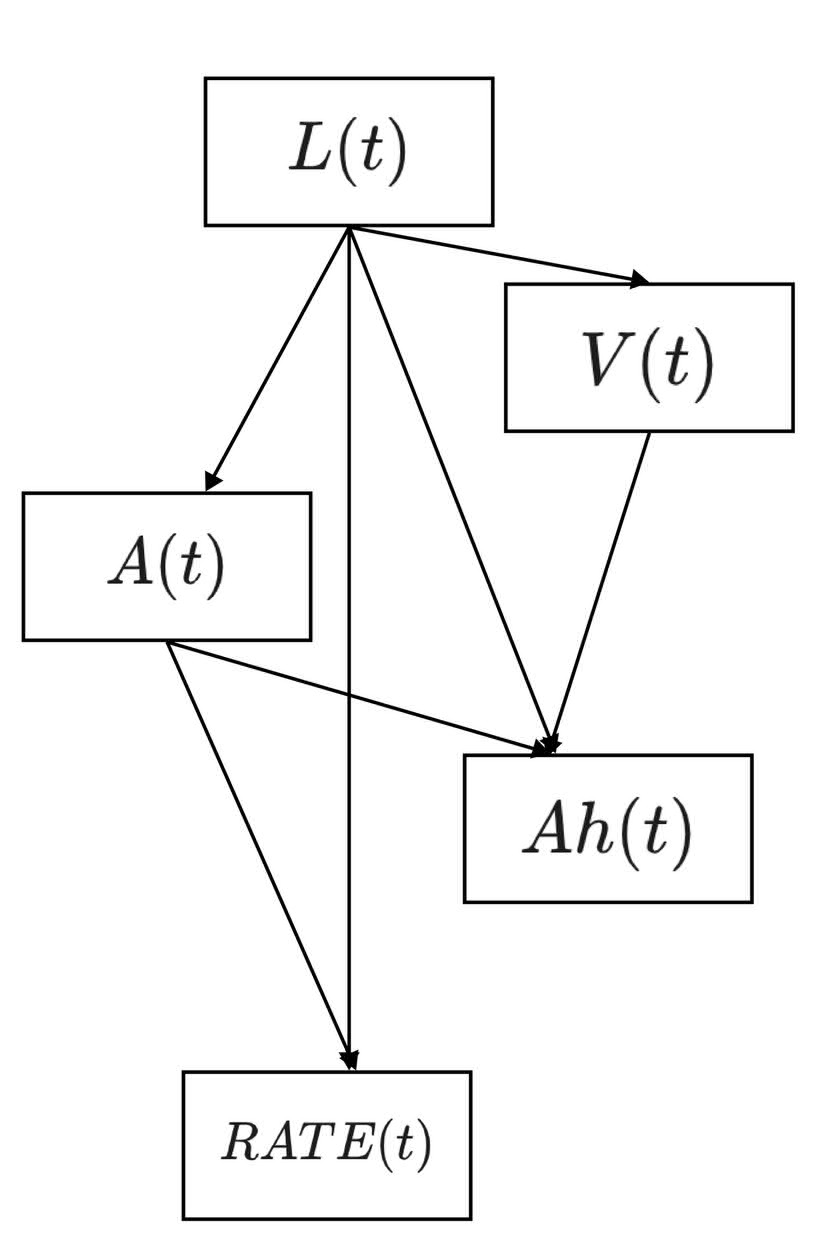
\includegraphics[width=195.75pt,height=298.2pt]{latexImage_f9adfc823effe6b2d2f11610c7139f42.png}}
\put(389.1,-519.911){\fontsize{11}{1}\usefont{T1}{ptm}{m}{n}\selectfont\color{color_29791} }
\put(78,-543.311){\fontsize{11}{1}\usefont{T1}{cmr}{m}{n}\selectfont\color{color_80434}¡}
\put(118.8,-543.311){\fontsize{11}{1}\usefont{T1}{cmr}{m}{n}\selectfont\color{color_80434}为}
\put(134.4,-543.311){\fontsize{11}{1}\usefont{T1}{cmr}{m}{n}\selectfont\color{color_80434}时}
\put(145.4,-543.311){\fontsize{11}{1}\usefont{T1}{cmr}{m}{n}\selectfont\color{color_80434}刻深度}
\put(178.4,-543.311){\fontsize{11}{1}\usefont{T1}{cmr}{m}{n}\selectfont\color{color_80434},}
\put(214.9,-543.311){\fontsize{11}{1}\usefont{T1}{cmr}{m}{n}\selectfont\color{color_80434}为}
\put(230.5,-543.311){\fontsize{11}{1}\usefont{T1}{cmr}{m}{n}\selectfont\color{color_80434}时}
\put(241.5,-543.311){\fontsize{11}{1}\usefont{T1}{cmr}{m}{n}\selectfont\color{color_80434}刻速度}
\put(274.5,-543.311){\fontsize{11}{1}\usefont{T1}{cmr}{m}{n}\selectfont\color{color_80434},}
\put(311,-543.311){\fontsize{11}{1}\usefont{T1}{cmr}{m}{n}\selectfont\color{color_80434}为}
\put(392.6,-543.311){\fontsize{11}{1}\usefont{T1}{cmr}{m}{n}\selectfont\color{color_80434} }
\put(326.6,-543.311){\fontsize{11}{1}\usefont{T1}{cmr}{m}{n}\selectfont\color{color_80434}时}
\put(337.6,-543.311){\fontsize{11}{1}\usefont{T1}{cmr}{m}{n}\selectfont\color{color_80434}刻}
\put(348.6,-543.311){\fontsize{11}{1}\usefont{T1}{cmr}{m}{n}\selectfont\color{color_80434}加}
\put(359.6,-543.311){\fontsize{11}{1}\usefont{T1}{cmr}{m}{n}\selectfont\color{color_80434}速度}
\put(381.6,-543.311){\fontsize{11}{1}\usefont{T1}{cmr}{m}{n}\selectfont\color{color_80434},}
\put(429.1,-543.311){\fontsize{11}{1}\usefont{T1}{cmr}{m}{n}\selectfont\color{color_80434}为}
\put(444.7,-543.311){\fontsize{11}{1}\usefont{T1}{cmr}{m}{n}\selectfont\color{color_80434}时}
\put(455.7,-543.311){\fontsize{11}{1}\usefont{T1}{cmr}{m}{n}\selectfont\color{color_80434}刻升降}
\put(488.7,-543.311){\fontsize{11}{1}\usefont{T1}{cmr}{m}{n}\selectfont\color{color_80434}率}
\put(128.3,-566.811){\fontsize{11}{1}\usefont{T1}{cmr}{m}{n}\selectfont\color{color_80434}为}
\put(143.9,-566.811){\fontsize{11}{1}\usefont{T1}{cmr}{m}{n}\selectfont\color{color_80434}时}
\put(154.9,-566.811){\fontsize{11}{1}\usefont{T1}{cmr}{m}{n}\selectfont\color{color_80434}刻转弯}
\put(187.9,-566.811){\fontsize{11}{1}\usefont{T1}{cmr}{m}{n}\selectfont\color{color_80434}率}
\end{picture}
\newpage
\begin{tikzpicture}[overlay]\path(0pt,0pt);\end{tikzpicture}
\begin{picture}(-5,0)(2.5,0)
\put(56,-72.711){\fontsize{12}{1}\usefont{T1}{cmr}{m}{n}\selectfont\color{color_80434}由}
\put(68,-72.711){\fontsize{12}{1}\usefont{T1}{cmr}{m}{n}\selectfont\color{color_80434}上}
\put(80,-72.711){\fontsize{12}{1}\usefont{T1}{cmr}{m}{n}\selectfont\color{color_80434}图}
\put(92,-72.711){\fontsize{12}{1}\usefont{T1}{cmr}{m}{n}\selectfont\color{color_80434}可}
\put(104,-72.711){\fontsize{12}{1}\usefont{T1}{cmr}{m}{n}\selectfont\color{color_80434}知}
\put(314.2,-72.711){\fontsize{11}{1}\usefont{T1}{cmr}{m}{n}\selectfont\color{color_29791} }
\put(350.687,-72.711){\fontsize{11}{1}\usefont{T1}{cmr}{m}{n}\selectfont\color{color_29791} }
\put(116.2,-72.711){\fontsize{11}{1}\usefont{T1}{cmr}{m}{n}\selectfont\color{color_29791},给定当}
\put(160.2,-72.711){\fontsize{11}{1}\usefont{T1}{cmr}{m}{n}\selectfont\color{color_29791}前}
\put(171.2,-72.711){\fontsize{11}{1}\usefont{T1}{cmr}{m}{n}\selectfont\color{color_29791}时}
\put(182.2,-72.711){\fontsize{11}{1}\usefont{T1}{cmr}{m}{n}\selectfont\color{color_29791}刻深度}
\put(215.2,-72.711){\fontsize{11}{1}\usefont{T1}{cmr}{m}{n}\selectfont\color{color_29791}、加}
\put(237.2,-72.711){\fontsize{11}{1}\usefont{T1}{cmr}{m}{n}\selectfont\color{color_29791}速度}
\put(259.2,-72.711){\fontsize{11}{1}\usefont{T1}{cmr}{m}{n}\selectfont\color{color_29791}、}
\put(270.2,-72.711){\fontsize{11}{1}\usefont{T1}{cmr}{m}{n}\selectfont\color{color_29791}升降}
\put(292.2,-72.711){\fontsize{11}{1}\usefont{T1}{cmr}{m}{n}\selectfont\color{color_29791}率、}
\put(317.7,-72.711){\fontsize{11}{1}\usefont{T1}{cmr}{m}{n}\selectfont\color{color_29791}转弯}
\put(339.7,-72.711){\fontsize{11}{1}\usefont{T1}{cmr}{m}{n}\selectfont\color{color_29791}率}
\put(354.2,-72.711){\fontsize{11}{1}\usefont{T1}{cmr}{m}{n}\selectfont\color{color_29791}4}
\put(365.2,-72.711){\fontsize{11}{1}\usefont{T1}{cmr}{m}{n}\selectfont\color{color_29791}个变}
\put(387.2,-72.711){\fontsize{11}{1}\usefont{T1}{cmr}{m}{n}\selectfont\color{color_29791}量值}
\put(409.2,-72.711){\fontsize{11}{1}\usefont{T1}{cmr}{m}{n}\selectfont\color{color_29791},根据动态贝叶斯网}
\put(56,-85.81097){\fontsize{11}{1}\usefont{T1}{cmr}{m}{n}\selectfont\color{color_29791}络及}
\put(78,-85.81097){\fontsize{11}{1}\usefont{T1}{cmr}{m}{n}\selectfont\color{color_29791}各}
\put(89,-85.81097){\fontsize{11}{1}\usefont{T1}{cmr}{m}{n}\selectfont\color{color_29791}个变}
\put(111,-85.81097){\fontsize{11}{1}\usefont{T1}{cmr}{m}{n}\selectfont\color{color_29791}量}
\put(122,-85.81097){\fontsize{11}{1}\usefont{T1}{cmr}{m}{n}\selectfont\color{color_29791}的}
\put(133,-85.81097){\fontsize{11}{1}\usefont{T1}{cmr}{m}{n}\selectfont\color{color_29791}条件}
\put(155,-85.81097){\fontsize{11}{1}\usefont{T1}{cmr}{m}{n}\selectfont\color{color_29791}概率}
\put(177,-85.81097){\fontsize{11}{1}\usefont{T1}{cmr}{m}{n}\selectfont\color{color_29791}矩阵}
\put(199,-85.81097){\fontsize{11}{1}\usefont{T1}{cmr}{m}{n}\selectfont\color{color_29791},即可}
\put(232,-85.81097){\fontsize{11}{1}\usefont{T1}{cmr}{m}{n}\selectfont\color{color_29791}实}
\put(243,-85.81097){\fontsize{11}{1}\usefont{T1}{cmr}{m}{n}\selectfont\color{color_29791}现下一时}
\put(287,-85.81097){\fontsize{11}{1}\usefont{T1}{cmr}{m}{n}\selectfont\color{color_29791}刻航}
\put(309,-85.81097){\fontsize{11}{1}\usefont{T1}{cmr}{m}{n}\selectfont\color{color_29791}迹}
\put(320,-85.81097){\fontsize{11}{1}\usefont{T1}{cmr}{m}{n}\selectfont\color{color_29791}预测和}
\put(353,-85.81097){\fontsize{11}{1}\usefont{T1}{cmr}{m}{n}\selectfont\color{color_29791}生}
\put(364,-85.81097){\fontsize{11}{1}\usefont{T1}{cmr}{m}{n}\selectfont\color{color_29791}成}
\put(375,-85.81097){\fontsize{11}{1}\usefont{T1}{ptm}{m}{n}\selectfont\color{color_29791}.}
\put(303.5,-117.311){\fontsize{11}{1}\usefont{T1}{cmr}{m}{n}\selectfont\color{color_29791} }
\put(56,-117.311){\fontsize{11}{1}\usefont{T1}{cmr}{m}{n}\selectfont\color{color_29791}基}
\put(67.187,-117.311){\fontsize{11}{1}\usefont{T1}{cmr}{m}{n}\selectfont\color{color_29791}于}
\put(78.5,-117.311){\fontsize{11}{1}\usefont{T1}{cmr}{m}{n}\selectfont\color{color_29791}前}
\put(89.7,-117.311){\fontsize{11}{1}\usefont{T1}{cmr}{m}{n}\selectfont\color{color_29791}文}
\put(101,-117.311){\fontsize{11}{1}\usefont{T1}{cmr}{m}{n}\selectfont\color{color_29791}航}
\put(112.2,-117.311){\fontsize{11}{1}\usefont{T1}{cmr}{m}{n}\selectfont\color{color_29791}迹}
\put(123.5,-117.311){\fontsize{11}{1}\usefont{T1}{cmr}{m}{n}\selectfont\color{color_29791}变}
\put(134.7,-117.311){\fontsize{11}{1}\usefont{T1}{cmr}{m}{n}\selectfont\color{color_29791}量}
\put(146,-117.311){\fontsize{11}{1}\usefont{T1}{cmr}{m}{n}\selectfont\color{color_29791}介}
\put(157.187,-117.311){\fontsize{11}{1}\usefont{T1}{cmr}{m}{n}\selectfont\color{color_29791}绍}
\put(168.473,-117.311){\fontsize{11}{1}\usefont{T1}{cmr}{m}{n}\selectfont\color{color_29791},}
\put(179.7,-117.311){\fontsize{11}{1}\usefont{T1}{cmr}{m}{n}\selectfont\color{color_29791}深}
\put(190.986,-117.311){\fontsize{11}{1}\usefont{T1}{cmr}{m}{n}\selectfont\color{color_29791}度}
\put(202.2,-117.311){\fontsize{11}{1}\usefont{T1}{cmr}{m}{n}\selectfont\color{color_29791}变}
\put(213.5,-117.311){\fontsize{11}{1}\usefont{T1}{cmr}{m}{n}\selectfont\color{color_29791}量}
\put(224.7,-117.311){\fontsize{11}{1}\usefont{T1}{cmr}{m}{n}\selectfont\color{color_29791}可}
\put(235.986,-117.311){\fontsize{11}{1}\usefont{T1}{cmr}{m}{n}\selectfont\color{color_29791}以}
\put(247.2,-117.311){\fontsize{11}{1}\usefont{T1}{cmr}{m}{n}\selectfont\color{color_29791}直}
\put(258.486,-117.311){\fontsize{11}{1}\usefont{T1}{cmr}{m}{n}\selectfont\color{color_29791}接}
\put(269.7,-117.311){\fontsize{11}{1}\usefont{T1}{cmr}{m}{n}\selectfont\color{color_29791}获}
\put(281,-117.311){\fontsize{11}{1}\usefont{T1}{cmr}{m}{n}\selectfont\color{color_29791}取}
\put(292.2,-117.311){\fontsize{11}{1}\usefont{T1}{cmr}{m}{n}\selectfont\color{color_29791},}
\put(307.2,-117.311){\fontsize{11}{1}\usefont{T1}{cmr}{m}{n}\selectfont\color{color_29791}速}
\put(318.486,-117.311){\fontsize{11}{1}\usefont{T1}{cmr}{m}{n}\selectfont\color{color_29791}度}
\put(329.7,-117.311){\fontsize{11}{1}\usefont{T1}{cmr}{m}{n}\selectfont\color{color_29791}、}
\put(340.986,-117.311){\fontsize{11}{1}\usefont{T1}{cmr}{m}{n}\selectfont\color{color_29791}加}
\put(352.2,-117.311){\fontsize{11}{1}\usefont{T1}{cmr}{m}{n}\selectfont\color{color_29791}速}
\put(363.486,-117.311){\fontsize{11}{1}\usefont{T1}{cmr}{m}{n}\selectfont\color{color_29791}度}
\put(374.7,-117.311){\fontsize{11}{1}\usefont{T1}{cmr}{m}{n}\selectfont\color{color_29791}、}
\put(386,-117.311){\fontsize{11}{1}\usefont{T1}{cmr}{m}{n}\selectfont\color{color_29791}转}
\put(397.187,-117.311){\fontsize{11}{1}\usefont{T1}{cmr}{m}{n}\selectfont\color{color_29791}弯}
\put(408.5,-117.311){\fontsize{11}{1}\usefont{T1}{cmr}{m}{n}\selectfont\color{color_29791}率}
\put(419.687,-117.311){\fontsize{11}{1}\usefont{T1}{cmr}{m}{n}\selectfont\color{color_29791}和}
\put(431,-117.311){\fontsize{11}{1}\usefont{T1}{cmr}{m}{n}\selectfont\color{color_29791}升}
\put(442.187,-117.311){\fontsize{11}{1}\usefont{T1}{cmr}{m}{n}\selectfont\color{color_29791}降}
\put(453.5,-117.311){\fontsize{11}{1}\usefont{T1}{cmr}{m}{n}\selectfont\color{color_29791}率}
\put(464.7,-117.311){\fontsize{11}{1}\usefont{T1}{cmr}{m}{n}\selectfont\color{color_29791}则}
\put(476,-117.311){\fontsize{11}{1}\usefont{T1}{cmr}{m}{n}\selectfont\color{color_29791}通}
\put(487.187,-117.311){\fontsize{11}{1}\usefont{T1}{cmr}{m}{n}\selectfont\color{color_29791}过}
\put(498.473,-117.311){\fontsize{11}{1}\usefont{T1}{cmr}{m}{n}\selectfont\color{color_29791}推}
\put(56,-130.111){\fontsize{11}{1}\usefont{T1}{cmr}{m}{n}\selectfont\color{color_29791}导}
\put(67,-130.111){\fontsize{11}{1}\usefont{T1}{cmr}{m}{n}\selectfont\color{color_29791}获}
\put(78,-130.111){\fontsize{11}{1}\usefont{T1}{cmr}{m}{n}\selectfont\color{color_29791}取}
\put(89,-130.111){\fontsize{11}{1}\usefont{T1}{cmr}{m}{n}\selectfont\color{color_29791}:}
\put(56,-145.911){\fontsize{11}{1}\usefont{T1}{ptm}{m}{n}\selectfont\color{color_29791}1}
\put(61.5,-145.911){\fontsize{11}{1}\usefont{T1}{cmr}{m}{n}\selectfont\color{color_29791})}
\put(72.5,-145.911){\fontsize{11}{1}\usefont{T1}{cmr}{m}{n}\selectfont\color{color_29791}速度}
\put(94.5,-145.911){\fontsize{11}{1}\usefont{T1}{cmr}{m}{n}\selectfont\color{color_29791}和加}
\put(116.5,-145.911){\fontsize{11}{1}\usefont{T1}{cmr}{m}{n}\selectfont\color{color_29791}速度}
\put(138.5,-145.911){\fontsize{11}{1}\usefont{T1}{cmr}{m}{n}\selectfont\color{color_29791}变}
\put(149.5,-145.911){\fontsize{11}{1}\usefont{T1}{cmr}{m}{n}\selectfont\color{color_29791}量}
\put(56,-161.711){\fontsize{11}{1}\usefont{T1}{cmr}{m}{n}\selectfont\color{color_29791}速度}
\put(78,-161.711){\fontsize{11}{1}\usefont{T1}{cmr}{m}{n}\selectfont\color{color_29791}通过}
\put(100,-161.711){\fontsize{11}{1}\usefont{T1}{cmr}{m}{n}\selectfont\color{color_29791}已知}
\put(122,-161.711){\fontsize{11}{1}\usefont{T1}{cmr}{m}{n}\selectfont\color{color_29791}速度}
\put(144,-161.711){\fontsize{11}{1}\usefont{T1}{cmr}{m}{n}\selectfont\color{color_29791}分}
\put(155,-161.711){\fontsize{11}{1}\usefont{T1}{cmr}{m}{n}\selectfont\color{color_29791}量整}
\put(177,-161.711){\fontsize{11}{1}\usefont{T1}{cmr}{m}{n}\selectfont\color{color_29791}合}
\put(188,-161.711){\fontsize{11}{1}\usefont{T1}{cmr}{m}{n}\selectfont\color{color_29791}获}
\put(199,-161.711){\fontsize{11}{1}\usefont{T1}{cmr}{m}{n}\selectfont\color{color_29791}得:}
\put(184.9,-192.111){\fontsize{11}{1}\usefont{T1}{ptm}{m}{n}\selectfont\color{color_29791} }
\put(187.595,-192.111){\fontsize{11}{1}\usefont{T1}{ptm}{m}{n}\selectfont\color{color_29791} }
\put(190.389,-192.111){\fontsize{11}{1}\usefont{T1}{ptm}{m}{n}\selectfont\color{color_29791} }
\put(56,-224.311){\fontsize{11}{1}\usefont{T1}{cmr}{m}{n}\selectfont\color{color_29791}上式}
\put(108.8,-224.311){\fontsize{11}{1}\usefont{T1}{cmr}{m}{n}\selectfont\color{color_29791}为}
\put(119.8,-224.311){\fontsize{11}{1}\usefont{T1}{cmr}{m}{n}\selectfont\color{color_29791}东}
\put(130.8,-224.311){\fontsize{11}{1}\usefont{T1}{cmr}{m}{n}\selectfont\color{color_29791}向}
\put(141.8,-224.311){\fontsize{11}{1}\usefont{T1}{cmr}{m}{n}\selectfont\color{color_29791}速度}
\put(163.8,-224.311){\fontsize{11}{1}\usefont{T1}{cmr}{m}{n}\selectfont\color{color_29791},}
\put(207.1,-224.311){\fontsize{11}{1}\usefont{T1}{cmr}{m}{n}\selectfont\color{color_29791}为}
\put(218.1,-224.311){\fontsize{11}{1}\usefont{T1}{cmr}{m}{n}\selectfont\color{color_29791}北}
\put(229.1,-224.311){\fontsize{11}{1}\usefont{T1}{cmr}{m}{n}\selectfont\color{color_29791}向}
\put(240.1,-224.311){\fontsize{11}{1}\usefont{T1}{cmr}{m}{n}\selectfont\color{color_29791}速度}
\put(262.1,-224.311){\fontsize{11}{1}\usefont{T1}{cmr}{m}{n}\selectfont\color{color_29791},}
\put(304.6,-224.311){\fontsize{11}{1}\usefont{T1}{cmr}{m}{n}\selectfont\color{color_29791}为地向}
\put(337.6,-224.311){\fontsize{11}{1}\usefont{T1}{cmr}{m}{n}\selectfont\color{color_29791}速度}
\put(56,-241.111){\fontsize{12}{1}\usefont{T1}{cmr}{m}{n}\selectfont\color{color_80434}对}
\put(68,-241.111){\fontsize{12}{1}\usefont{T1}{cmr}{m}{n}\selectfont\color{color_80434}前}
\put(80,-241.111){\fontsize{12}{1}\usefont{T1}{cmr}{m}{n}\selectfont\color{color_80434}后}
\put(92,-241.111){\fontsize{12}{1}\usefont{T1}{cmr}{m}{n}\selectfont\color{color_80434}两}
\put(104,-241.111){\fontsize{12}{1}\usefont{T1}{cmr}{m}{n}\selectfont\color{color_80434}个时}
\put(128,-241.111){\fontsize{12}{1}\usefont{T1}{cmr}{m}{n}\selectfont\color{color_80434}刻做差}
\put(164,-241.111){\fontsize{12}{1}\usefont{T1}{cmr}{m}{n}\selectfont\color{color_80434}可得加}
\put(200,-241.111){\fontsize{12}{1}\usefont{T1}{cmr}{m}{n}\selectfont\color{color_80434}速度}
\put(224,-241.111){\fontsize{12}{1}\usefont{T1}{cmr}{m}{n}\selectfont\color{color_80434}数}
\put(236,-241.111){\fontsize{12}{1}\usefont{T1}{cmr}{m}{n}\selectfont\color{color_80434}值}
\put(248,-241.111){\fontsize{12}{1}\usefont{T1}{cmr}{m}{n}\selectfont\color{color_80434}:}
\put(56,-291.511){\fontsize{12}{1}\usefont{T1}{ptm}{m}{n}\selectfont\color{color_80434}2)}
\put(72.8,-291.511){\fontsize{12}{1}\usefont{T1}{cmr}{m}{n}\selectfont\color{color_80434}升降}
\put(96.8,-291.511){\fontsize{12}{1}\usefont{T1}{cmr}{m}{n}\selectfont\color{color_80434}率变}
\put(120.8,-291.511){\fontsize{12}{1}\usefont{T1}{cmr}{m}{n}\selectfont\color{color_80434}量}
\put(72.8,-308.511){\fontsize{12}{1}\usefont{T1}{cmr}{m}{n}\selectfont\color{color_80434}通过对}
\put(108.8,-308.511){\fontsize{12}{1}\usefont{T1}{cmr}{m}{n}\selectfont\color{color_80434}前}
\put(120.8,-308.511){\fontsize{12}{1}\usefont{T1}{cmr}{m}{n}\selectfont\color{color_80434}后}
\put(135.2,-308.511){\fontsize{12}{1}\usefont{T1}{ptm}{m}{n}\selectfont\color{color_80434}2}
\put(143.6,-308.511){\fontsize{12}{1}\usefont{T1}{cmr}{m}{n}\selectfont\color{color_80434}个时}
\put(167.6,-308.511){\fontsize{12}{1}\usefont{T1}{cmr}{m}{n}\selectfont\color{color_80434}刻深度}
\put(203.6,-308.511){\fontsize{12}{1}\usefont{T1}{cmr}{m}{n}\selectfont\color{color_80434}数}
\put(215.6,-308.511){\fontsize{12}{1}\usefont{T1}{cmr}{m}{n}\selectfont\color{color_80434}值做差}
\put(251.6,-308.511){\fontsize{12}{1}\usefont{T1}{cmr}{m}{n}\selectfont\color{color_80434}可得:}
\put(56,-358.911){\fontsize{12}{1}\usefont{T1}{ptm}{m}{n}\selectfont\color{color_80434}3)}
\put(72.8,-358.911){\fontsize{12}{1}\usefont{T1}{cmr}{m}{n}\selectfont\color{color_80434}航}
\put(84.8,-358.911){\fontsize{12}{1}\usefont{T1}{cmr}{m}{n}\selectfont\color{color_80434}向}
\put(96.8,-358.911){\fontsize{12}{1}\usefont{T1}{cmr}{m}{n}\selectfont\color{color_80434}角}
\put(108.8,-358.911){\fontsize{12}{1}\usefont{T1}{cmr}{m}{n}\selectfont\color{color_80434}和}
\put(120.8,-358.911){\fontsize{12}{1}\usefont{T1}{cmr}{m}{n}\selectfont\color{color_80434}转弯}
\put(144.8,-358.911){\fontsize{12}{1}\usefont{T1}{cmr}{m}{n}\selectfont\color{color_80434}率变}
\put(168.8,-358.911){\fontsize{12}{1}\usefont{T1}{cmr}{m}{n}\selectfont\color{color_80434}量}
\put(72.8,-375.911){\fontsize{12}{1}\usefont{T1}{cmr}{m}{n}\selectfont\color{color_80434}将}
\put(85,-375.911){\fontsize{12}{1}\usefont{T1}{cmr}{m}{n}\selectfont\color{color_80434}东}
\put(97.2,-375.911){\fontsize{12}{1}\usefont{T1}{cmr}{m}{n}\selectfont\color{color_80434}向}
\put(109.4,-375.911){\fontsize{12}{1}\usefont{T1}{cmr}{m}{n}\selectfont\color{color_80434}速}
\put(121.592,-375.911){\fontsize{12}{1}\usefont{T1}{cmr}{m}{n}\selectfont\color{color_80434}度}
\put(133.8,-375.911){\fontsize{12}{1}\usefont{T1}{cmr}{m}{n}\selectfont\color{color_80434}和}
\put(146,-375.911){\fontsize{12}{1}\usefont{T1}{cmr}{m}{n}\selectfont\color{color_80434}北}
\put(158.2,-375.911){\fontsize{12}{1}\usefont{T1}{cmr}{m}{n}\selectfont\color{color_80434}向}
\put(170.4,-375.911){\fontsize{12}{1}\usefont{T1}{cmr}{m}{n}\selectfont\color{color_80434}速}
\put(182.592,-375.911){\fontsize{12}{1}\usefont{T1}{cmr}{m}{n}\selectfont\color{color_80434}度}
\put(194.784,-375.911){\fontsize{12}{1}\usefont{T1}{cmr}{m}{n}\selectfont\color{color_80434}做}
\put(207,-375.911){\fontsize{12}{1}\usefont{T1}{cmr}{m}{n}\selectfont\color{color_80434}比}
\put(219.192,-375.911){\fontsize{12}{1}\usefont{T1}{cmr}{m}{n}\selectfont\color{color_80434},}
\put(231.384,-375.911){\fontsize{12}{1}\usefont{T1}{cmr}{m}{n}\selectfont\color{color_80434}得}
\put(243.576,-375.911){\fontsize{12}{1}\usefont{T1}{cmr}{m}{n}\selectfont\color{color_80434}到}
\put(255.8,-375.911){\fontsize{12}{1}\usefont{T1}{cmr}{m}{n}\selectfont\color{color_80434}航}
\put(268,-375.911){\fontsize{12}{1}\usefont{T1}{cmr}{m}{n}\selectfont\color{color_80434}向}
\put(280.192,-375.911){\fontsize{12}{1}\usefont{T1}{cmr}{m}{n}\selectfont\color{color_80434}参}
\put(292.4,-375.911){\fontsize{12}{1}\usefont{T1}{cmr}{m}{n}\selectfont\color{color_80434}考}
\put(304.6,-375.911){\fontsize{12}{1}\usefont{T1}{cmr}{m}{n}\selectfont\color{color_80434}数}
\put(316.792,-375.911){\fontsize{12}{1}\usefont{T1}{cmr}{m}{n}\selectfont\color{color_80434}据}
\put(328.984,-375.911){\fontsize{12}{1}\usefont{T1}{cmr}{m}{n}\selectfont\color{color_80434},}
\put(341.176,-375.911){\fontsize{12}{1}\usefont{T1}{cmr}{m}{n}\selectfont\color{color_80434}设}
\put(353.368,-375.911){\fontsize{12}{1}\usefont{T1}{cmr}{m}{n}\selectfont\color{color_80434}定}
\put(365.6,-375.911){\fontsize{12}{1}\usefont{T1}{cmr}{m}{n}\selectfont\color{color_80434}北}
\put(377.8,-375.911){\fontsize{12}{1}\usefont{T1}{cmr}{m}{n}\selectfont\color{color_80434}为}
\put(400.6,-375.911){\fontsize{12}{1}\usefont{T1}{cmr}{m}{n}\selectfont\color{color_80434}轴}
\put(412.792,-375.911){\fontsize{12}{1}\usefont{T1}{cmr}{m}{n}\selectfont\color{color_80434}正}
\put(425,-375.911){\fontsize{12}{1}\usefont{T1}{cmr}{m}{n}\selectfont\color{color_80434}方}
\put(437.192,-375.911){\fontsize{12}{1}\usefont{T1}{cmr}{m}{n}\selectfont\color{color_80434}向}
\put(449.384,-375.911){\fontsize{12}{1}\usefont{T1}{cmr}{m}{n}\selectfont\color{color_80434},}
\put(461.6,-375.911){\fontsize{12}{1}\usefont{T1}{cmr}{m}{n}\selectfont\color{color_80434}东}
\put(473.8,-375.911){\fontsize{12}{1}\usefont{T1}{cmr}{m}{n}\selectfont\color{color_80434}为}
\put(497.5,-375.911){\fontsize{12}{1}\usefont{T1}{cmr}{m}{n}\selectfont\color{color_80434}轴}
\put(72.8,-389.911){\fontsize{12}{1}\usefont{T1}{cmr}{m}{n}\selectfont\color{color_80434}正}
\put(84.8,-389.911){\fontsize{12}{1}\usefont{T1}{cmr}{m}{n}\selectfont\color{color_80434}方向,将}
\put(132.8,-389.911){\fontsize{12}{1}\usefont{T1}{cmr}{m}{n}\selectfont\color{color_80434}航}
\put(144.8,-389.911){\fontsize{12}{1}\usefont{T1}{cmr}{m}{n}\selectfont\color{color_80434}向参}
\put(168.8,-389.911){\fontsize{12}{1}\usefont{T1}{cmr}{m}{n}\selectfont\color{color_80434}考}
\put(180.8,-389.911){\fontsize{12}{1}\usefont{T1}{cmr}{m}{n}\selectfont\color{color_80434}数据}
\put(204.8,-389.911){\fontsize{12}{1}\usefont{T1}{cmr}{m}{n}\selectfont\color{color_80434}转}
\put(216.8,-389.911){\fontsize{12}{1}\usefont{T1}{cmr}{m}{n}\selectfont\color{color_80434}换}
\put(228.8,-389.911){\fontsize{12}{1}\usefont{T1}{cmr}{m}{n}\selectfont\color{color_80434}成}
\put(240.8,-389.911){\fontsize{12}{1}\usefont{T1}{cmr}{m}{n}\selectfont\color{color_80434}坐}
\put(252.8,-389.911){\fontsize{12}{1}\usefont{T1}{cmr}{m}{n}\selectfont\color{color_80434}标系下的}
\put(300.8,-389.911){\fontsize{12}{1}\usefont{T1}{cmr}{m}{n}\selectfont\color{color_80434}航}
\put(312.8,-389.911){\fontsize{12}{1}\usefont{T1}{cmr}{m}{n}\selectfont\color{color_80434}向}
\put(324.8,-389.911){\fontsize{12}{1}\usefont{T1}{cmr}{m}{n}\selectfont\color{color_80434}角}
\put(77.8,-480.511){\fontsize{12}{1}\usefont{T1}{cmr}{m}{n}\selectfont\color{color_80434}为潜水器的}
\put(137.8,-480.511){\fontsize{12}{1}\usefont{T1}{cmr}{m}{n}\selectfont\color{color_80434}坐}
\put(149.8,-480.511){\fontsize{12}{1}\usefont{T1}{cmr}{m}{n}\selectfont\color{color_80434}标系}
\put(173.8,-480.511){\fontsize{12}{1}\usefont{T1}{cmr}{m}{n}\selectfont\color{color_80434}航}
\put(185.8,-480.511){\fontsize{12}{1}\usefont{T1}{cmr}{m}{n}\selectfont\color{color_80434}向}
\put(197.8,-480.511){\fontsize{12}{1}\usefont{T1}{cmr}{m}{n}\selectfont\color{color_80434}角}
\put(56,-516.711){\fontsize{12}{1}\usefont{T1}{cmr}{m}{n}\selectfont\color{color_80434}若}
\put(98.8,-516.711){\fontsize{12}{1}\usefont{T1}{ptm}{m}{n}\selectfont\color{color_80434}>}
\put(105.496,-516.711){\fontsize{12}{1}\usefont{T1}{ptm}{m}{n}\selectfont\color{color_80434}0}
\put(111.5,-516.711){\fontsize{12}{1}\usefont{T1}{cmr}{m}{n}\selectfont\color{color_80434},}
\put(155.8,-516.711){\fontsize{12}{1}\usefont{T1}{ptm}{m}{n}\selectfont\color{color_80434}>}
\put(162.592,-516.711){\fontsize{12}{1}\usefont{T1}{ptm}{m}{n}\selectfont\color{color_80434}0 ,}
\put(174.6,-516.711){\fontsize{12}{1}\usefont{T1}{cmr}{m}{n}\selectfont\color{color_80434}则}
\put(208.4,-516.711){\fontsize{12}{1}\usefont{T1}{ptm}{m}{n}\selectfont\color{color_80434}=}
\put(236.9,-516.711){\fontsize{12}{1}\usefont{T1}{cmr}{m}{n}\selectfont\color{color_80434};若}
\put(291.7,-516.711){\fontsize{12}{1}\usefont{T1}{ptm}{m}{n}\selectfont\color{color_80434}<}
\put(298.492,-516.711){\fontsize{12}{1}\usefont{T1}{ptm}{m}{n}\selectfont\color{color_80434}0,}
\put(339.8,-516.711){\fontsize{12}{1}\usefont{T1}{ptm}{m}{n}\selectfont\color{color_80434}>}
\put(346.496,-516.711){\fontsize{12}{1}\usefont{T1}{ptm}{m}{n}\selectfont\color{color_80434}0 ,}
\put(358.5,-516.711){\fontsize{12}{1}\usefont{T1}{cmr}{m}{n}\selectfont\color{color_80434}则}
\put(392.3,-516.711){\fontsize{12}{1}\usefont{T1}{ptm}{m}{n}\selectfont\color{color_80434}=}
\put(462.9,-516.711){\fontsize{12}{1}\usefont{T1}{cmr}{m}{n}\selectfont\color{color_80434};}
\put(56,-536.111){\fontsize{12}{1}\usefont{T1}{cmr}{m}{n}\selectfont\color{color_80434}若}
\put(98.8,-536.111){\fontsize{12}{1}\usefont{T1}{ptm}{m}{n}\selectfont\color{color_80434}>}
\put(105.496,-536.111){\fontsize{12}{1}\usefont{T1}{ptm}{m}{n}\selectfont\color{color_80434}0 ,}
\put(149.8,-536.111){\fontsize{12}{1}\usefont{T1}{ptm}{m}{n}\selectfont\color{color_80434}<}
\put(156.592,-536.111){\fontsize{12}{1}\usefont{T1}{ptm}{m}{n}\selectfont\color{color_80434}0 ,}
\put(168.6,-536.111){\fontsize{12}{1}\usefont{T1}{cmr}{m}{n}\selectfont\color{color_80434}则}
\put(202.4,-536.111){\fontsize{12}{1}\usefont{T1}{cmr}{m}{n}\selectfont\color{color_80434} }
\put(206.2,-536.111){\fontsize{12}{1}\usefont{T1}{ptm}{m}{n}\selectfont\color{color_80434}=}
\put(276.7,-536.111){\fontsize{12}{1}\usefont{T1}{ptm}{m}{n}\selectfont\color{color_80434} ;}
\put(283.1,-536.111){\fontsize{12}{1}\usefont{T1}{cmr}{m}{n}\selectfont\color{color_80434}若}
\put(325.9,-536.111){\fontsize{12}{1}\usefont{T1}{ptm}{m}{n}\selectfont\color{color_80434}<}
\put(332.596,-536.111){\fontsize{12}{1}\usefont{T1}{ptm}{m}{n}\selectfont\color{color_80434}0,}
\put(373.9,-536.111){\fontsize{12}{1}\usefont{T1}{ptm}{m}{n}\selectfont\color{color_80434}<}
\put(380.692,-536.111){\fontsize{12}{1}\usefont{T1}{ptm}{m}{n}\selectfont\color{color_80434}0, }
\put(392.7,-536.111){\fontsize{12}{1}\usefont{T1}{cmr}{m}{n}\selectfont\color{color_80434}则}
\put(426.5,-536.111){\fontsize{12}{1}\usefont{T1}{ptm}{m}{n}\selectfont\color{color_80434}=}
\put(56,-572.311){\fontsize{12}{1}\usefont{T1}{cmr}{m}{n}\selectfont\color{color_80434}进而计算}
\put(104,-572.311){\fontsize{12}{1}\usefont{T1}{cmr}{m}{n}\selectfont\color{color_80434}转弯}
\put(128,-572.311){\fontsize{12}{1}\usefont{T1}{cmr}{m}{n}\selectfont\color{color_80434}率}
\put(140,-572.311){\fontsize{12}{1}\usefont{T1}{ptm}{m}{n}\selectfont\color{color_80434},}
\put(56,-605.211){\fontsize{12}{1}\usefont{T1}{cmr}{m}{n}\selectfont\color{color_80434}}
\put(72.8,-605.211){\fontsize{11}{1}\usefont{T1}{cmr}{m}{n}\selectfont\color{color_29791}针}
\put(84,-605.211){\fontsize{11}{1}\usefont{T1}{cmr}{m}{n}\selectfont\color{color_29791}对}
\put(95.187,-605.211){\fontsize{11}{1}\usefont{T1}{cmr}{m}{n}\selectfont\color{color_29791}潜}
\put(106.374,-605.211){\fontsize{11}{1}\usefont{T1}{cmr}{m}{n}\selectfont\color{color_29791}水}
\put(117.561,-605.211){\fontsize{11}{1}\usefont{T1}{cmr}{m}{n}\selectfont\color{color_29791}器}
\put(128.8,-605.211){\fontsize{11}{1}\usefont{T1}{cmr}{m}{n}\selectfont\color{color_29791}升}
\put(139.987,-605.211){\fontsize{11}{1}\usefont{T1}{cmr}{m}{n}\selectfont\color{color_29791}降}
\put(151.2,-605.211){\fontsize{11}{1}\usefont{T1}{cmr}{m}{n}\selectfont\color{color_29791}率}
\put(162.387,-605.211){\fontsize{11}{1}\usefont{T1}{cmr}{m}{n}\selectfont\color{color_29791}、}
\put(173.6,-605.211){\fontsize{11}{1}\usefont{T1}{cmr}{m}{n}\selectfont\color{color_29791}转}
\put(184.787,-605.211){\fontsize{11}{1}\usefont{T1}{cmr}{m}{n}\selectfont\color{color_29791}弯}
\put(196,-605.211){\fontsize{11}{1}\usefont{T1}{cmr}{m}{n}\selectfont\color{color_29791}率}
\put(207.187,-605.211){\fontsize{11}{1}\usefont{T1}{cmr}{m}{n}\selectfont\color{color_29791}和}
\put(218.374,-605.211){\fontsize{11}{1}\usefont{T1}{cmr}{m}{n}\selectfont\color{color_29791}加}
\put(229.6,-605.211){\fontsize{11}{1}\usefont{T1}{cmr}{m}{n}\selectfont\color{color_29791}速}
\put(240.787,-605.211){\fontsize{11}{1}\usefont{T1}{cmr}{m}{n}\selectfont\color{color_29791}度}
\put(252,-605.211){\fontsize{11}{1}\usefont{T1}{cmr}{m}{n}\selectfont\color{color_29791},}
\put(263.2,-605.211){\fontsize{11}{1}\usefont{T1}{cmr}{m}{n}\selectfont\color{color_29791}均}
\put(274.4,-605.211){\fontsize{11}{1}\usefont{T1}{cmr}{m}{n}\selectfont\color{color_29791}可}
\put(285.587,-605.211){\fontsize{11}{1}\usefont{T1}{cmr}{m}{n}\selectfont\color{color_29791}建}
\put(296.774,-605.211){\fontsize{11}{1}\usefont{T1}{cmr}{m}{n}\selectfont\color{color_29791}立}
\put(308,-605.211){\fontsize{11}{1}\usefont{T1}{cmr}{m}{n}\selectfont\color{color_29791}类}
\put(319.2,-605.211){\fontsize{11}{1}\usefont{T1}{cmr}{m}{n}\selectfont\color{color_29791}似}
\put(330.387,-605.211){\fontsize{11}{1}\usefont{T1}{cmr}{m}{n}\selectfont\color{color_29791}条}
\put(341.574,-605.211){\fontsize{11}{1}\usefont{T1}{cmr}{m}{n}\selectfont\color{color_29791}件}
\put(352.8,-605.211){\fontsize{11}{1}\usefont{T1}{cmr}{m}{n}\selectfont\color{color_29791}概}
\put(363.987,-605.211){\fontsize{11}{1}\usefont{T1}{cmr}{m}{n}\selectfont\color{color_29791}率}
\put(375.2,-605.211){\fontsize{11}{1}\usefont{T1}{cmr}{m}{n}\selectfont\color{color_29791}矩}
\put(386.387,-605.211){\fontsize{11}{1}\usefont{T1}{cmr}{m}{n}\selectfont\color{color_29791}阵}
\put(397.6,-605.211){\fontsize{11}{1}\usefont{T1}{cmr}{m}{n}\selectfont\color{color_29791}。}
\put(408.787,-605.211){\fontsize{11}{1}\usefont{T1}{cmr}{m}{n}\selectfont\color{color_29791}在}
\put(419.974,-605.211){\fontsize{11}{1}\usefont{T1}{cmr}{m}{n}\selectfont\color{color_29791}之}
\put(431.161,-605.211){\fontsize{11}{1}\usefont{T1}{cmr}{m}{n}\selectfont\color{color_29791}后}
\put(442.4,-605.211){\fontsize{11}{1}\usefont{T1}{cmr}{m}{n}\selectfont\color{color_29791}迭}
\put(453.587,-605.211){\fontsize{11}{1}\usefont{T1}{cmr}{m}{n}\selectfont\color{color_29791}代}
\put(464.8,-605.211){\fontsize{11}{1}\usefont{T1}{cmr}{m}{n}\selectfont\color{color_29791}过}
\put(475.987,-605.211){\fontsize{11}{1}\usefont{T1}{cmr}{m}{n}\selectfont\color{color_29791}程}
\put(487.174,-605.211){\fontsize{11}{1}\usefont{T1}{cmr}{m}{n}\selectfont\color{color_29791}中}
\put(498.361,-605.211){\fontsize{11}{1}\usefont{T1}{cmr}{m}{n}\selectfont\color{color_29791},}
\put(72.8,-618.011){\fontsize{11}{1}\usefont{T1}{cmr}{m}{n}\selectfont\color{color_29791}通过}
\put(94.8,-618.011){\fontsize{11}{1}\usefont{T1}{cmr}{m}{n}\selectfont\color{color_29791}调}
\put(105.8,-618.011){\fontsize{11}{1}\usefont{T1}{cmr}{m}{n}\selectfont\color{color_29791}用变}
\put(127.8,-618.011){\fontsize{11}{1}\usefont{T1}{cmr}{m}{n}\selectfont\color{color_29791}量}
\put(138.8,-618.011){\fontsize{11}{1}\usefont{T1}{cmr}{m}{n}\selectfont\color{color_29791}条件}
\put(160.8,-618.011){\fontsize{11}{1}\usefont{T1}{cmr}{m}{n}\selectfont\color{color_29791}概率}
\put(182.8,-618.011){\fontsize{11}{1}\usefont{T1}{cmr}{m}{n}\selectfont\color{color_29791}矩阵}
\put(204.8,-618.011){\fontsize{11}{1}\usefont{T1}{cmr}{m}{n}\selectfont\color{color_29791},}
\put(215.8,-618.011){\fontsize{11}{1}\usefont{T1}{cmr}{m}{n}\selectfont\color{color_29791}依}
\put(226.8,-618.011){\fontsize{11}{1}\usefont{T1}{cmr}{m}{n}\selectfont\color{color_29791}照子节}
\put(259.8,-618.011){\fontsize{11}{1}\usefont{T1}{cmr}{m}{n}\selectfont\color{color_29791}点}
\put(270.8,-618.011){\fontsize{11}{1}\usefont{T1}{cmr}{m}{n}\selectfont\color{color_29791}取值}
\put(292.8,-618.011){\fontsize{11}{1}\usefont{T1}{cmr}{m}{n}\selectfont\color{color_29791}概率分布}
\put(336.8,-618.011){\fontsize{11}{1}\usefont{T1}{cmr}{m}{n}\selectfont\color{color_29791}生}
\put(347.8,-618.011){\fontsize{11}{1}\usefont{T1}{cmr}{m}{n}\selectfont\color{color_29791}成预测}
\put(380.8,-618.011){\fontsize{11}{1}\usefont{T1}{cmr}{m}{n}\selectfont\color{color_29791}值}
\put(391.8,-618.011){\fontsize{11}{1}\usefont{T1}{ptm}{m}{n}\selectfont\color{color_29791}.}
\put(56,-633.811){\fontsize{12}{1}\usefont{T1}{cmr}{m}{n}\selectfont\color{color_80434}}
\put(72.8,-633.811){\fontsize{12}{1}\usefont{T1}{ptm}{m}{n}\selectfont\color{color_29791} }
\put(76,-633.811){\fontsize{11}{1}\usefont{T1}{cmr}{m}{n}\selectfont\color{color_29791}针}
\put(87.1,-633.811){\fontsize{11}{1}\usefont{T1}{cmr}{m}{n}\selectfont\color{color_29791}对}
\put(98.188,-633.811){\fontsize{11}{1}\usefont{T1}{cmr}{m}{n}\selectfont\color{color_29791}预}
\put(109.276,-633.811){\fontsize{11}{1}\usefont{T1}{cmr}{m}{n}\selectfont\color{color_29791}测}
\put(120.364,-633.811){\fontsize{11}{1}\usefont{T1}{cmr}{m}{n}\selectfont\color{color_29791}得}
\put(131.452,-633.811){\fontsize{11}{1}\usefont{T1}{cmr}{m}{n}\selectfont\color{color_29791}到}
\put(142.54,-633.811){\fontsize{11}{1}\usefont{T1}{cmr}{m}{n}\selectfont\color{color_29791}的}
\put(153.628,-633.811){\fontsize{11}{1}\usefont{T1}{cmr}{m}{n}\selectfont\color{color_29791}潜}
\put(164.716,-633.811){\fontsize{11}{1}\usefont{T1}{cmr}{m}{n}\selectfont\color{color_29791}水}
\put(175.804,-633.811){\fontsize{11}{1}\usefont{T1}{cmr}{m}{n}\selectfont\color{color_29791}器}
\put(187,-633.811){\fontsize{11}{1}\usefont{T1}{cmr}{m}{n}\selectfont\color{color_29791}航}
\put(198.1,-633.811){\fontsize{11}{1}\usefont{T1}{cmr}{m}{n}\selectfont\color{color_29791}迹}
\put(209.2,-633.811){\fontsize{11}{1}\usefont{T1}{cmr}{m}{n}\selectfont\color{color_29791}数}
\put(220.288,-633.811){\fontsize{11}{1}\usefont{T1}{cmr}{m}{n}\selectfont\color{color_29791}据}
\put(231.376,-633.811){\fontsize{11}{1}\usefont{T1}{cmr}{m}{n}\selectfont\color{color_29791},}
\put(242.464,-633.811){\fontsize{11}{1}\usefont{T1}{cmr}{m}{n}\selectfont\color{color_29791}进}
\put(253.552,-633.811){\fontsize{11}{1}\usefont{T1}{cmr}{m}{n}\selectfont\color{color_29791}行}
\put(264.64,-633.811){\fontsize{11}{1}\usefont{T1}{cmr}{m}{n}\selectfont\color{color_29791}可}
\put(275.8,-633.811){\fontsize{11}{1}\usefont{T1}{cmr}{m}{n}\selectfont\color{color_29791}视}
\put(286.9,-633.811){\fontsize{11}{1}\usefont{T1}{cmr}{m}{n}\selectfont\color{color_29791}化}
\put(298,-633.811){\fontsize{11}{1}\usefont{T1}{cmr}{m}{n}\selectfont\color{color_29791}处}
\put(309.1,-633.811){\fontsize{11}{1}\usefont{T1}{cmr}{m}{n}\selectfont\color{color_29791}理}
\put(320.188,-633.811){\fontsize{11}{1}\usefont{T1}{cmr}{m}{n}\selectfont\color{color_29791},}
\put(331.276,-633.811){\fontsize{11}{1}\usefont{T1}{cmr}{m}{n}\selectfont\color{color_29791}建}
\put(342.364,-633.811){\fontsize{11}{1}\usefont{T1}{cmr}{m}{n}\selectfont\color{color_29791}立}
\put(353.4521,-633.811){\fontsize{11}{1}\usefont{T1}{cmr}{m}{n}\selectfont\color{color_29791}三}
\put(364.5401,-633.811){\fontsize{11}{1}\usefont{T1}{cmr}{m}{n}\selectfont\color{color_29791}维}
\put(375.7,-633.811){\fontsize{11}{1}\usefont{T1}{cmr}{m}{n}\selectfont\color{color_29791}坐}
\put(386.8,-633.811){\fontsize{11}{1}\usefont{T1}{cmr}{m}{n}\selectfont\color{color_29791}标}
\put(397.888,-633.811){\fontsize{11}{1}\usefont{T1}{cmr}{m}{n}\selectfont\color{color_29791}系}
\put(408.976,-633.811){\fontsize{11}{1}\usefont{T1}{cmr}{m}{n}\selectfont\color{color_29791}。}
\put(420.1,-633.811){\fontsize{11}{1}\usefont{T1}{cmr}{m}{n}\selectfont\color{color_29791}其}
\put(431.2,-633.811){\fontsize{11}{1}\usefont{T1}{cmr}{m}{n}\selectfont\color{color_29791}中}
\put(442.288,-633.811){\fontsize{11}{1}\usefont{T1}{cmr}{m}{n}\selectfont\color{color_29791},}
\put(453.4,-633.811){\fontsize{11}{1}\usefont{T1}{cmr}{m}{n}\selectfont\color{color_29791}Z}
\put(464.5,-633.811){\fontsize{11}{1}\usefont{T1}{cmr}{m}{n}\selectfont\color{color_29791}轴}
\put(475.588,-633.811){\fontsize{11}{1}\usefont{T1}{cmr}{m}{n}\selectfont\color{color_29791}取}
\put(486.676,-633.811){\fontsize{11}{1}\usefont{T1}{cmr}{m}{n}\selectfont\color{color_29791}值}
\put(497.8,-633.811){\fontsize{11}{1}\usefont{T1}{cmr}{m}{n}\selectfont\color{color_29791}地}
\put(139.4,-646.711){\fontsize{11}{1}\usefont{T1}{cmr}{m}{n}\selectfont\color{color_29791} }
\put(376.087,-646.711){\fontsize{11}{1}\usefont{T1}{cmr}{m}{n}\selectfont\color{color_29791} }
\put(72.8,-646.711){\fontsize{11}{1}\usefont{T1}{cmr}{m}{n}\selectfont\color{color_29791}面}
\put(83.9,-646.711){\fontsize{11}{1}\usefont{T1}{cmr}{m}{n}\selectfont\color{color_29791}垂}
\put(95,-646.711){\fontsize{11}{1}\usefont{T1}{cmr}{m}{n}\selectfont\color{color_29791}直}
\put(106.1,-646.711){\fontsize{11}{1}\usefont{T1}{cmr}{m}{n}\selectfont\color{color_29791}向}
\put(117.188,-646.711){\fontsize{11}{1}\usefont{T1}{cmr}{m}{n}\selectfont\color{color_29791}上}
\put(128.276,-646.711){\fontsize{11}{1}\usefont{T1}{cmr}{m}{n}\selectfont\color{color_29791}为}
\put(143,-646.711){\fontsize{11}{1}\usefont{T1}{cmr}{m}{n}\selectfont\color{color_29791}正}
\put(154.1,-646.711){\fontsize{11}{1}\usefont{T1}{cmr}{m}{n}\selectfont\color{color_29791},}
\put(165.2,-646.711){\fontsize{11}{1}\usefont{T1}{cmr}{m}{n}\selectfont\color{color_29791}X}
\put(176.3,-646.711){\fontsize{11}{1}\usefont{T1}{cmr}{m}{n}\selectfont\color{color_29791}轴}
\put(187.388,-646.711){\fontsize{11}{1}\usefont{T1}{cmr}{m}{n}\selectfont\color{color_29791}取}
\put(198.476,-646.711){\fontsize{11}{1}\usefont{T1}{cmr}{m}{n}\selectfont\color{color_29791}值}
\put(209.6,-646.711){\fontsize{11}{1}\usefont{T1}{cmr}{m}{n}\selectfont\color{color_29791}向}
\put(220.7,-646.711){\fontsize{11}{1}\usefont{T1}{cmr}{m}{n}\selectfont\color{color_29791}东}
\put(231.8,-646.711){\fontsize{11}{1}\usefont{T1}{cmr}{m}{n}\selectfont\color{color_29791}为}
\put(242.9,-646.711){\fontsize{11}{1}\usefont{T1}{cmr}{m}{n}\selectfont\color{color_29791}正}
\put(254,-646.711){\fontsize{11}{1}\usefont{T1}{cmr}{m}{n}\selectfont\color{color_29791},}
\put(265.1,-646.711){\fontsize{11}{1}\usefont{T1}{cmr}{m}{n}\selectfont\color{color_29791}Y}
\put(276.2,-646.711){\fontsize{11}{1}\usefont{T1}{cmr}{m}{n}\selectfont\color{color_29791}轴}
\put(287.288,-646.711){\fontsize{11}{1}\usefont{T1}{cmr}{m}{n}\selectfont\color{color_29791}取}
\put(298.376,-646.711){\fontsize{11}{1}\usefont{T1}{cmr}{m}{n}\selectfont\color{color_29791}值}
\put(309.5,-646.711){\fontsize{11}{1}\usefont{T1}{cmr}{m}{n}\selectfont\color{color_29791}向}
\put(320.6,-646.711){\fontsize{11}{1}\usefont{T1}{cmr}{m}{n}\selectfont\color{color_29791}北}
\put(331.7,-646.711){\fontsize{11}{1}\usefont{T1}{cmr}{m}{n}\selectfont\color{color_29791}为}
\put(342.8,-646.711){\fontsize{11}{1}\usefont{T1}{cmr}{m}{n}\selectfont\color{color_29791}正}
\put(353.9,-646.711){\fontsize{11}{1}\usefont{T1}{cmr}{m}{n}\selectfont\color{color_29791}。}
\put(364.988,-646.711){\fontsize{11}{1}\usefont{T1}{cmr}{m}{n}\selectfont\color{color_29791}在}
\put(379.7,-646.711){\fontsize{11}{1}\usefont{T1}{cmr}{m}{n}\selectfont\color{color_29791}X}
\put(391.2,-646.711){\fontsize{11}{1}\usefont{T1}{ptm}{m}{n}\selectfont\color{color_29791}-}
\put(428.2,-646.711){\fontsize{11}{1}\usefont{T1}{cmr}{m}{n}\selectfont\color{color_29791} }
\put(394.9,-646.711){\fontsize{11}{1}\usefont{T1}{cmr}{m}{n}\selectfont\color{color_29791}Y}
\put(406,-646.711){\fontsize{11}{1}\usefont{T1}{cmr}{m}{n}\selectfont\color{color_29791}平}
\put(417.1,-646.711){\fontsize{11}{1}\usefont{T1}{cmr}{m}{n}\selectfont\color{color_29791}面}
\put(431.785,-646.711){\fontsize{11}{1}\usefont{T1}{cmr}{m}{n}\selectfont\color{color_29791}上}
\put(442.873,-646.711){\fontsize{11}{1}\usefont{T1}{cmr}{m}{n}\selectfont\color{color_29791},}
\put(453.961,-646.711){\fontsize{11}{1}\usefont{T1}{cmr}{m}{n}\selectfont\color{color_29791}设}
\put(465.049,-646.711){\fontsize{11}{1}\usefont{T1}{cmr}{m}{n}\selectfont\color{color_29791}定}
\put(476.2,-646.711){\fontsize{11}{1}\usefont{T1}{cmr}{m}{n}\selectfont\color{color_29791}航}
\put(487.3,-646.711){\fontsize{11}{1}\usefont{T1}{cmr}{m}{n}\selectfont\color{color_29791}向}
\put(498.4,-646.711){\fontsize{11}{1}\usefont{T1}{cmr}{m}{n}\selectfont\color{color_29791}初}
\put(261.5,-659.511){\fontsize{11}{1}\usefont{T1}{cmr}{m}{n}\selectfont\color{color_29791} }
\put(72.8,-659.511){\fontsize{11}{1}\usefont{T1}{cmr}{m}{n}\selectfont\color{color_29791}始}
\put(83.888,-659.511){\fontsize{11}{1}\usefont{T1}{cmr}{m}{n}\selectfont\color{color_29791}值}
\put(95,-659.511){\fontsize{11}{1}\usefont{T1}{cmr}{m}{n}\selectfont\color{color_29791},}
\put(106.088,-659.511){\fontsize{11}{1}\usefont{T1}{cmr}{m}{n}\selectfont\color{color_29791}将}
\put(117.176,-659.511){\fontsize{11}{1}\usefont{T1}{cmr}{m}{n}\selectfont\color{color_29791}预}
\put(128.264,-659.511){\fontsize{11}{1}\usefont{T1}{cmr}{m}{n}\selectfont\color{color_29791}测}
\put(139.352,-659.511){\fontsize{11}{1}\usefont{T1}{cmr}{m}{n}\selectfont\color{color_29791}出}
\put(150.5,-659.511){\fontsize{11}{1}\usefont{T1}{cmr}{m}{n}\selectfont\color{color_29791}来}
\put(161.6,-659.511){\fontsize{11}{1}\usefont{T1}{cmr}{m}{n}\selectfont\color{color_29791}的}
\put(172.7,-659.511){\fontsize{11}{1}\usefont{T1}{cmr}{m}{n}\selectfont\color{color_29791}转}
\put(183.788,-659.511){\fontsize{11}{1}\usefont{T1}{cmr}{m}{n}\selectfont\color{color_29791}弯}
\put(194.9,-659.511){\fontsize{11}{1}\usefont{T1}{cmr}{m}{n}\selectfont\color{color_29791}率}
\put(205.988,-659.511){\fontsize{11}{1}\usefont{T1}{cmr}{m}{n}\selectfont\color{color_29791}变}
\put(217.076,-659.511){\fontsize{11}{1}\usefont{T1}{cmr}{m}{n}\selectfont\color{color_29791}化}
\put(228.2,-659.511){\fontsize{11}{1}\usefont{T1}{cmr}{m}{n}\selectfont\color{color_29791}量}
\put(239.3,-659.511){\fontsize{11}{1}\usefont{T1}{cmr}{m}{n}\selectfont\color{color_29791}不}
\put(250.4,-659.511){\fontsize{11}{1}\usefont{T1}{cmr}{m}{n}\selectfont\color{color_29791}断}
\put(265.085,-659.511){\fontsize{11}{1}\usefont{T1}{cmr}{m}{n}\selectfont\color{color_29791}叠}
\put(276.2,-659.511){\fontsize{11}{1}\usefont{T1}{cmr}{m}{n}\selectfont\color{color_29791}加}
\put(287.288,-659.511){\fontsize{11}{1}\usefont{T1}{cmr}{m}{n}\selectfont\color{color_29791},}
\put(298.4,-659.511){\fontsize{11}{1}\usefont{T1}{cmr}{m}{n}\selectfont\color{color_29791}迭}
\put(309.488,-659.511){\fontsize{11}{1}\usefont{T1}{cmr}{m}{n}\selectfont\color{color_29791}代}
\put(320.6,-659.511){\fontsize{11}{1}\usefont{T1}{cmr}{m}{n}\selectfont\color{color_29791}生}
\put(331.7,-659.511){\fontsize{11}{1}\usefont{T1}{cmr}{m}{n}\selectfont\color{color_29791}成}
\put(342.8,-659.511){\fontsize{11}{1}\usefont{T1}{cmr}{m}{n}\selectfont\color{color_29791}航}
\put(353.9,-659.511){\fontsize{11}{1}\usefont{T1}{cmr}{m}{n}\selectfont\color{color_29791}向}
\put(364.988,-659.511){\fontsize{11}{1}\usefont{T1}{cmr}{m}{n}\selectfont\color{color_29791}新}
\put(376.1,-659.511){\fontsize{11}{1}\usefont{T1}{cmr}{m}{n}\selectfont\color{color_29791}值}
\put(387.2,-659.511){\fontsize{11}{1}\usefont{T1}{cmr}{m}{n}\selectfont\color{color_29791}。}
\put(398.288,-659.511){\fontsize{11}{1}\usefont{T1}{cmr}{m}{n}\selectfont\color{color_29791}基}
\put(409.376,-659.511){\fontsize{11}{1}\usefont{T1}{cmr}{m}{n}\selectfont\color{color_29791}于}
\put(420.5,-659.511){\fontsize{11}{1}\usefont{T1}{cmr}{m}{n}\selectfont\color{color_29791}运}
\put(431.6,-659.511){\fontsize{11}{1}\usefont{T1}{cmr}{m}{n}\selectfont\color{color_29791}动}
\put(442.688,-659.511){\fontsize{11}{1}\usefont{T1}{cmr}{m}{n}\selectfont\color{color_29791}学}
\put(453.776,-659.511){\fontsize{11}{1}\usefont{T1}{cmr}{m}{n}\selectfont\color{color_29791}方}
\put(464.864,-659.511){\fontsize{11}{1}\usefont{T1}{cmr}{m}{n}\selectfont\color{color_29791}程}
\put(475.9521,-659.511){\fontsize{11}{1}\usefont{T1}{cmr}{m}{n}\selectfont\color{color_29791},}
\put(487.1,-659.511){\fontsize{11}{1}\usefont{T1}{cmr}{m}{n}\selectfont\color{color_29791}生}
\put(498.2,-659.511){\fontsize{11}{1}\usefont{T1}{cmr}{m}{n}\selectfont\color{color_29791}成}
\put(116.8,-672.311){\fontsize{11}{1}\usefont{T1}{cmr}{m}{n}\selectfont\color{color_29791} }
\put(72.8,-672.311){\fontsize{11}{1}\usefont{T1}{cmr}{m}{n}\selectfont\color{color_29791}潜水器在}
\put(120.3,-672.311){\fontsize{11}{1}\usefont{T1}{cmr}{m}{n}\selectfont\color{color_29791}X}
\put(131.3,-672.311){\fontsize{11}{1}\usefont{T1}{cmr}{m}{n}\selectfont\color{color_29791}轴}
\put(142.3,-672.311){\fontsize{11}{1}\usefont{T1}{cmr}{m}{n}\selectfont\color{color_29791}、}
\put(153.3,-672.311){\fontsize{11}{1}\usefont{T1}{cmr}{m}{n}\selectfont\color{color_29791}Y}
\put(164.3,-672.311){\fontsize{11}{1}\usefont{T1}{cmr}{m}{n}\selectfont\color{color_29791}轴}
\put(175.3,-672.311){\fontsize{11}{1}\usefont{T1}{cmr}{m}{n}\selectfont\color{color_29791}、}
\put(186.3,-672.311){\fontsize{11}{1}\usefont{T1}{cmr}{m}{n}\selectfont\color{color_29791}Z}
\put(197.3,-672.311){\fontsize{11}{1}\usefont{T1}{cmr}{m}{n}\selectfont\color{color_29791}轴}
\put(208.3,-672.311){\fontsize{11}{1}\usefont{T1}{cmr}{m}{n}\selectfont\color{color_29791}的}
\put(219.3,-672.311){\fontsize{11}{1}\usefont{T1}{cmr}{m}{n}\selectfont\color{color_29791}实}
\put(230.3,-672.311){\fontsize{11}{1}\usefont{T1}{cmr}{m}{n}\selectfont\color{color_29791}时位置}
\put(263.3,-672.311){\fontsize{11}{1}\usefont{T1}{ptm}{m}{n}\selectfont\color{color_29791}:}
\end{picture}
\newpage
\begin{tikzpicture}[overlay]\path(0pt,0pt);\end{tikzpicture}
\begin{picture}(-5,0)(2.5,0)
\put(56,-151.311){\fontsize{12}{1}\usefont{T1}{cmr}{m}{n}\selectfont\color{color_80434}上}
\put(68.288,-151.311){\fontsize{12}{1}\usefont{T1}{cmr}{m}{n}\selectfont\color{color_80434}式}
\put(80.576,-151.311){\fontsize{12}{1}\usefont{T1}{cmr}{m}{n}\selectfont\color{color_80434}中}
\put(92.9,-151.311){\fontsize{12}{1}\usefont{T1}{ptm}{m}{n}\selectfont\color{color_80434},}
\put(118.4,-151.311){\fontsize{12}{1}\usefont{T1}{cmr}{m}{n}\selectfont\color{color_80434}为}
\put(130.688,-151.311){\fontsize{12}{1}\usefont{T1}{cmr}{m}{n}\selectfont\color{color_80434}潜}
\put(142.976,-151.311){\fontsize{12}{1}\usefont{T1}{cmr}{m}{n}\selectfont\color{color_80434}水}
\put(155.264,-151.311){\fontsize{12}{1}\usefont{T1}{cmr}{m}{n}\selectfont\color{color_80434}器}
\put(167.552,-151.311){\fontsize{12}{1}\usefont{T1}{cmr}{m}{n}\selectfont\color{color_80434}在}
\put(191.2,-151.311){\fontsize{12}{1}\usefont{T1}{cmr}{m}{n}\selectfont\color{color_80434}轴}
\put(203.488,-151.311){\fontsize{12}{1}\usefont{T1}{cmr}{m}{n}\selectfont\color{color_80434}坐}
\put(215.8,-151.311){\fontsize{12}{1}\usefont{T1}{cmr}{m}{n}\selectfont\color{color_80434}标}
\put(228.1,-151.311){\fontsize{12}{1}\usefont{T1}{ptm}{m}{n}\selectfont\color{color_80434};}
\put(253.3,-151.311){\fontsize{12}{1}\usefont{T1}{cmr}{m}{n}\selectfont\color{color_80434}为}
\put(265.588,-151.311){\fontsize{12}{1}\usefont{T1}{cmr}{m}{n}\selectfont\color{color_80434}潜}
\put(277.876,-151.311){\fontsize{12}{1}\usefont{T1}{cmr}{m}{n}\selectfont\color{color_80434}水}
\put(290.164,-151.311){\fontsize{12}{1}\usefont{T1}{cmr}{m}{n}\selectfont\color{color_80434}器}
\put(302.452,-151.311){\fontsize{12}{1}\usefont{T1}{cmr}{m}{n}\selectfont\color{color_80434}在}
\put(324.6,-151.311){\fontsize{12}{1}\usefont{T1}{cmr}{m}{n}\selectfont\color{color_80434}轴}
\put(336.888,-151.311){\fontsize{12}{1}\usefont{T1}{cmr}{m}{n}\selectfont\color{color_80434}坐}
\put(349.2,-151.311){\fontsize{12}{1}\usefont{T1}{cmr}{m}{n}\selectfont\color{color_80434}标}
\put(361.5,-151.311){\fontsize{12}{1}\usefont{T1}{ptm}{m}{n}\selectfont\color{color_80434};}
\put(386.6,-151.311){\fontsize{12}{1}\usefont{T1}{cmr}{m}{n}\selectfont\color{color_80434}为}
\put(398.888,-151.311){\fontsize{12}{1}\usefont{T1}{cmr}{m}{n}\selectfont\color{color_80434}潜}
\put(411.176,-151.311){\fontsize{12}{1}\usefont{T1}{cmr}{m}{n}\selectfont\color{color_80434}水}
\put(423.464,-151.311){\fontsize{12}{1}\usefont{T1}{cmr}{m}{n}\selectfont\color{color_80434}器}
\put(435.752,-151.311){\fontsize{12}{1}\usefont{T1}{cmr}{m}{n}\selectfont\color{color_80434}在}
\put(457.9,-151.311){\fontsize{12}{1}\usefont{T1}{cmr}{m}{n}\selectfont\color{color_80434}轴}
\put(470.188,-151.311){\fontsize{12}{1}\usefont{T1}{cmr}{m}{n}\selectfont\color{color_80434}坐}
\put(482.5,-151.311){\fontsize{12}{1}\usefont{T1}{cmr}{m}{n}\selectfont\color{color_80434}标}
\put(494.8,-151.311){\fontsize{12}{1}\usefont{T1}{ptm}{m}{n}\selectfont\color{color_80434};}
\put(56,-165.311){\fontsize{12}{1}\usefont{T1}{cmr}{m}{n}\selectfont\color{color_80434}为潜水器}
\put(104,-165.311){\fontsize{12}{1}\usefont{T1}{cmr}{m}{n}\selectfont\color{color_80434}初始航}
\put(140,-165.311){\fontsize{12}{1}\usefont{T1}{cmr}{m}{n}\selectfont\color{color_80434}向}
\put(152,-165.311){\fontsize{12}{1}\usefont{T1}{ptm}{m}{n}\selectfont\color{color_80434},}
\put(155,-165.311){\fontsize{12}{1}\usefont{T1}{cmr}{m}{n}\selectfont\color{color_80434}如下}
\put(179,-165.311){\fontsize{12}{1}\usefont{T1}{cmr}{m}{n}\selectfont\color{color_80434}图}
\put(104.55,-529.111){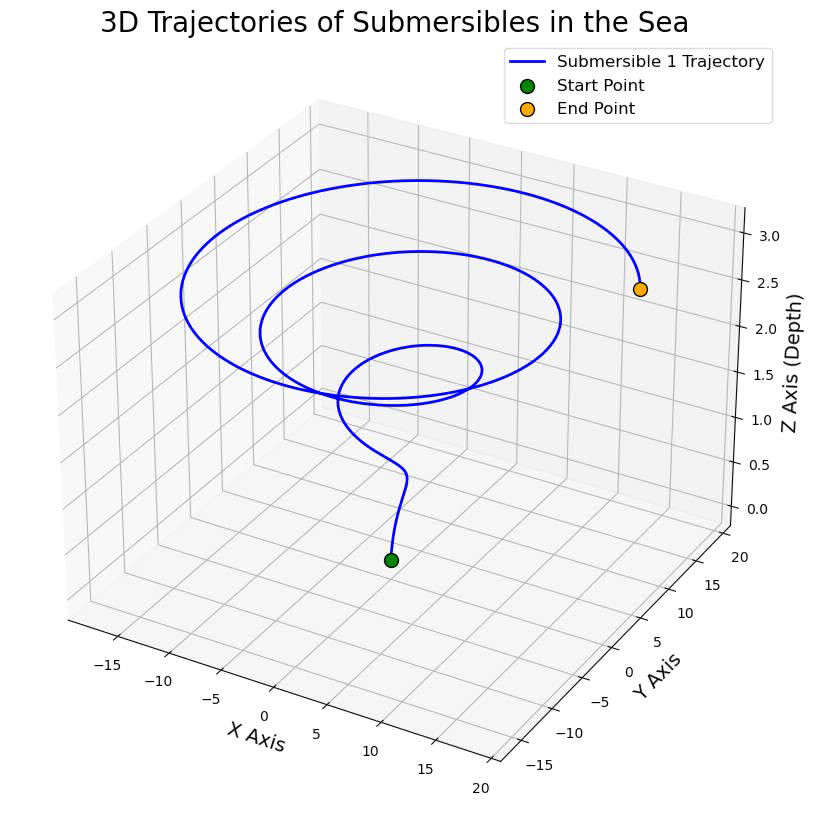
\includegraphics[width=356.25pt,height=358pt]{latexImage_259b76769763bdf74890f1cd3c713364.png}}
\put(56,-581.511){\fontsize{11}{1}\usefont{T1}{cmr}{m}{n}\selectfont\color{color_80434}}
\put(72.8,-581.511){\fontsize{11}{1}\usefont{T1}{cmr}{m}{n}\selectfont\color{color_80434}假}
\put(83.8,-581.511){\fontsize{11}{1}\usefont{T1}{cmr}{m}{n}\selectfont\color{color_80434}设模型}
\put(56,-598.311){\fontsize{12}{1}\usefont{T1}{cmr}{m}{n}\selectfont\color{color_80434}我}
\put(68,-598.311){\fontsize{12}{1}\usefont{T1}{cmr}{m}{n}\selectfont\color{color_80434}们}
\put(80,-598.311){\fontsize{12}{1}\usefont{T1}{cmr}{m}{n}\selectfont\color{color_80434}生}
\put(92,-598.311){\fontsize{12}{1}\usefont{T1}{cmr}{m}{n}\selectfont\color{color_80434}成简}
\put(116,-598.311){\fontsize{12}{1}\usefont{T1}{cmr}{m}{n}\selectfont\color{color_80434}单}
\put(128,-598.311){\fontsize{12}{1}\usefont{T1}{cmr}{m}{n}\selectfont\color{color_80434}的模拟数据}
\put(188,-598.311){\fontsize{12}{1}\usefont{T1}{cmr}{m}{n}\selectfont\color{color_80434}来}
\put(200,-598.311){\fontsize{12}{1}\usefont{T1}{cmr}{m}{n}\selectfont\color{color_80434}观}
\put(212,-598.311){\fontsize{12}{1}\usefont{T1}{cmr}{m}{n}\selectfont\color{color_80434}察}
\put(224,-598.311){\fontsize{12}{1}\usefont{T1}{cmr}{m}{n}\selectfont\color{color_80434}主船和潜水器的}
\put(308,-598.311){\fontsize{12}{1}\usefont{T1}{cmr}{m}{n}\selectfont\color{color_80434}路}
\put(320,-598.311){\fontsize{12}{1}\usefont{T1}{cmr}{m}{n}\selectfont\color{color_80434}径}
\put(332,-598.311){\fontsize{12}{1}\usefont{T1}{cmr}{m}{n}\selectfont\color{color_80434},}
\put(344,-598.311){\fontsize{12}{1}\usefont{T1}{cmr}{m}{n}\selectfont\color{color_80434}再}
\put(356,-598.311){\fontsize{12}{1}\usefont{T1}{cmr}{m}{n}\selectfont\color{color_80434}构}
\put(368,-598.311){\fontsize{12}{1}\usefont{T1}{cmr}{m}{n}\selectfont\color{color_80434}建}
\put(380,-598.311){\fontsize{12}{1}\usefont{T1}{cmr}{m}{n}\selectfont\color{color_80434}特}
\put(392,-598.311){\fontsize{12}{1}\usefont{T1}{cmr}{m}{n}\selectfont\color{color_80434}征}
\put(404,-598.311){\fontsize{12}{1}\usefont{T1}{cmr}{m}{n}\selectfont\color{color_80434}和标}
\put(428,-598.311){\fontsize{12}{1}\usefont{T1}{cmr}{m}{n}\selectfont\color{color_80434}签}
\put(440,-598.311){\fontsize{12}{1}\usefont{T1}{cmr}{m}{n}\selectfont\color{color_80434},}
\put(452,-598.311){\fontsize{12}{1}\usefont{T1}{ptm}{m}{n}\selectfont\color{color_80434}0}
\put(460.4,-598.311){\fontsize{12}{1}\usefont{T1}{cmr}{m}{n}\selectfont\color{color_80434}表}
\put(472.4,-598.311){\fontsize{12}{1}\usefont{T1}{cmr}{m}{n}\selectfont\color{color_80434}示}
\put(484.4,-598.311){\fontsize{12}{1}\usefont{T1}{cmr}{m}{n}\selectfont\color{color_80434}主船}
\put(508.4,-598.311){\fontsize{12}{1}\usefont{T1}{cmr}{m}{n}\selectfont\color{color_80434},}
\put(56,-612.411){\fontsize{12}{1}\usefont{T1}{ptm}{m}{n}\selectfont\color{color_80434}1}
\put(64.4,-612.411){\fontsize{12}{1}\usefont{T1}{cmr}{m}{n}\selectfont\color{color_80434}表}
\put(76.4,-612.411){\fontsize{12}{1}\usefont{T1}{cmr}{m}{n}\selectfont\color{color_80434}示}
\put(88.4,-612.411){\fontsize{12}{1}\usefont{T1}{cmr}{m}{n}\selectfont\color{color_80434}潜水器,}
\put(136.4,-612.411){\fontsize{12}{1}\usefont{T1}{cmr}{m}{n}\selectfont\color{color_80434}然}
\put(148.4,-612.411){\fontsize{12}{1}\usefont{T1}{cmr}{m}{n}\selectfont\color{color_80434}后}
\put(160.4,-612.411){\fontsize{12}{1}\usefont{T1}{cmr}{m}{n}\selectfont\color{color_80434}我}
\put(172.4,-612.411){\fontsize{12}{1}\usefont{T1}{cmr}{m}{n}\selectfont\color{color_80434}们使用贝叶斯网络分}
\put(280.4,-612.411){\fontsize{12}{1}\usefont{T1}{cmr}{m}{n}\selectfont\color{color_80434}类}
\put(292.4,-612.411){\fontsize{12}{1}\usefont{T1}{cmr}{m}{n}\selectfont\color{color_80434}进行}
\put(316.4,-612.411){\fontsize{12}{1}\usefont{T1}{cmr}{m}{n}\selectfont\color{color_80434}训}
\put(328.4,-612.411){\fontsize{12}{1}\usefont{T1}{cmr}{m}{n}\selectfont\color{color_80434}练}
\put(340.4,-612.411){\fontsize{12}{1}\usefont{T1}{cmr}{m}{n}\selectfont\color{color_80434},}
\put(352.4,-612.411){\fontsize{12}{1}\usefont{T1}{cmr}{m}{n}\selectfont\color{color_80434}构}
\put(364.4,-612.411){\fontsize{12}{1}\usefont{T1}{cmr}{m}{n}\selectfont\color{color_80434}建网格}
\put(400.4,-612.411){\fontsize{12}{1}\usefont{T1}{cmr}{m}{n}\selectfont\color{color_80434}来}
\put(412.4,-612.411){\fontsize{12}{1}\usefont{T1}{cmr}{m}{n}\selectfont\color{color_80434}绘}
\put(424.4,-612.411){\fontsize{12}{1}\usefont{T1}{cmr}{m}{n}\selectfont\color{color_80434}制}
\put(436.4,-612.411){\fontsize{12}{1}\usefont{T1}{cmr}{m}{n}\selectfont\color{color_80434}决策}
\put(460.4,-612.411){\fontsize{12}{1}\usefont{T1}{cmr}{m}{n}\selectfont\color{color_80434}边界}
\put(484.4,-612.411){\fontsize{12}{1}\usefont{T1}{cmr}{m}{n}\selectfont\color{color_80434},}
\put(496.4,-612.411){\fontsize{12}{1}\usefont{T1}{cmr}{m}{n}\selectfont\color{color_80434}得}
\put(56,-626.411){\fontsize{12}{1}\usefont{T1}{cmr}{m}{n}\selectfont\color{color_80434}到主船和潜水器的}
\put(152,-626.411){\fontsize{12}{1}\usefont{T1}{cmr}{m}{n}\selectfont\color{color_80434}路}
\put(164,-626.411){\fontsize{12}{1}\usefont{T1}{cmr}{m}{n}\selectfont\color{color_80434}径图}
\put(188,-626.411){\fontsize{12}{1}\usefont{T1}{cmr}{m}{n}\selectfont\color{color_80434},这个}
\put(224,-626.411){\fontsize{12}{1}\usefont{T1}{cmr}{m}{n}\selectfont\color{color_80434}只}
\put(236,-626.411){\fontsize{12}{1}\usefont{T1}{cmr}{m}{n}\selectfont\color{color_80434}是我}
\put(260,-626.411){\fontsize{12}{1}\usefont{T1}{cmr}{m}{n}\selectfont\color{color_80434}们简}
\put(284,-626.411){\fontsize{12}{1}\usefont{T1}{cmr}{m}{n}\selectfont\color{color_80434}单}
\put(296,-626.411){\fontsize{12}{1}\usefont{T1}{cmr}{m}{n}\selectfont\color{color_80434}的模拟}
\put(179.9,-646.311){\fontsize{11}{1}\usefont{T1}{ptm}{m}{n}\selectfont\color{color_80434}s}
\put(184.19,-646.311){\fontsize{11}{1}\usefont{T1}{ptm}{m}{n}\selectfont\color{color_80434}h}
\put(189.591,-646.311){\fontsize{11}{1}\usefont{T1}{ptm}{m}{n}\selectfont\color{color_80434}i}
\put(192.682,-646.311){\fontsize{11}{1}\usefont{T1}{ptm}{m}{n}\selectfont\color{color_80434}p\_pa}
\put(214.066,-646.311){\fontsize{11}{1}\usefont{T1}{ptm}{m}{n}\selectfont\color{color_80434}t}
\put(217.157,-646.311){\fontsize{11}{1}\usefont{T1}{ptm}{m}{n}\selectfont\color{color_80434}h}
\put(233.7,-646.311){\fontsize{11}{1}\usefont{T1}{cmr}{m}{n}\selectfont\color{color_80434} }
\put(222.7,-646.311){\fontsize{11}{1}\usefont{T1}{cmr}{m}{n}\selectfont\color{color_80434}:}
\put(237.2,-646.311){\fontsize{11}{1}\usefont{T1}{ptm}{m}{n}\selectfont\color{color_80434}[}
\put(240.797,-646.311){\fontsize{11}{1}\usefont{T1}{ptm}{m}{n}\selectfont\color{color_80434}[}
\put(244.482,-646.311){\fontsize{11}{1}\usefont{T1}{ptm}{m}{n}\selectfont\color{color_80434}1,}
\put(252.776,-646.311){\fontsize{11}{1}\usefont{T1}{ptm}{m}{n}\selectfont\color{color_80434} }
\put(255.471,-646.311){\fontsize{11}{1}\usefont{T1}{ptm}{m}{n}\selectfont\color{color_80434}2]}
\put(264.568,-646.311){\fontsize{11}{1}\usefont{T1}{ptm}{m}{n}\selectfont\color{color_80434},}
\put(267.362,-646.311){\fontsize{11}{1}\usefont{T1}{ptm}{m}{n}\selectfont\color{color_80434} }
\put(270.156,-646.311){\fontsize{11}{1}\usefont{T1}{ptm}{m}{n}\selectfont\color{color_80434}[}
\put(273.753,-646.311){\fontsize{11}{1}\usefont{T1}{ptm}{m}{n}\selectfont\color{color_80434}2,}
\put(282.047,-646.311){\fontsize{11}{1}\usefont{T1}{ptm}{m}{n}\selectfont\color{color_80434} }
\put(284.742,-646.311){\fontsize{11}{1}\usefont{T1}{ptm}{m}{n}\selectfont\color{color_80434}3]}
\put(293.927,-646.311){\fontsize{11}{1}\usefont{T1}{ptm}{m}{n}\selectfont\color{color_80434},}
\put(296.721,-646.311){\fontsize{11}{1}\usefont{T1}{ptm}{m}{n}\selectfont\color{color_80434} }
\put(299.416,-646.311){\fontsize{11}{1}\usefont{T1}{ptm}{m}{n}\selectfont\color{color_80434}[}
\put(303.101,-646.311){\fontsize{11}{1}\usefont{T1}{ptm}{m}{n}\selectfont\color{color_80434}3}
\put(308.502,-646.311){\fontsize{11}{1}\usefont{T1}{ptm}{m}{n}\selectfont\color{color_80434},}
\put(311.296,-646.311){\fontsize{11}{1}\usefont{T1}{ptm}{m}{n}\selectfont\color{color_80434} }
\put(314.09,-646.311){\fontsize{11}{1}\usefont{T1}{ptm}{m}{n}\selectfont\color{color_80434}4}
\put(319.491,-646.311){\fontsize{11}{1}\usefont{T1}{ptm}{m}{n}\selectfont\color{color_80434}]}
\put(323.176,-646.311){\fontsize{11}{1}\usefont{T1}{ptm}{m}{n}\selectfont\color{color_80434},}
\put(325.97,-646.311){\fontsize{11}{1}\usefont{T1}{ptm}{m}{n}\selectfont\color{color_80434} }
\put(328.665,-646.311){\fontsize{11}{1}\usefont{T1}{ptm}{m}{n}\selectfont\color{color_80434}[}
\put(332.35,-646.311){\fontsize{11}{1}\usefont{T1}{ptm}{m}{n}\selectfont\color{color_80434}4,}
\put(340.644,-646.311){\fontsize{11}{1}\usefont{T1}{ptm}{m}{n}\selectfont\color{color_80434} }
\put(343.3391,-646.311){\fontsize{11}{1}\usefont{T1}{ptm}{m}{n}\selectfont\color{color_80434}5]}
\put(352.436,-646.311){\fontsize{11}{1}\usefont{T1}{ptm}{m}{n}\selectfont\color{color_80434},}
\put(355.23,-646.311){\fontsize{11}{1}\usefont{T1}{ptm}{m}{n}\selectfont\color{color_80434} }
\put(358.024,-646.311){\fontsize{11}{1}\usefont{T1}{ptm}{m}{n}\selectfont\color{color_80434}[}
\put(361.621,-646.311){\fontsize{11}{1}\usefont{T1}{ptm}{m}{n}\selectfont\color{color_80434}5,}
\put(369.915,-646.311){\fontsize{11}{1}\usefont{T1}{ptm}{m}{n}\selectfont\color{color_80434} }
\put(372.61,-646.311){\fontsize{11}{1}\usefont{T1}{ptm}{m}{n}\selectfont\color{color_80434}6]}
\put(381.795,-646.311){\fontsize{11}{1}\usefont{T1}{ptm}{m}{n}\selectfont\color{color_80434}]}
\put(166.1,-666.011){\fontsize{11}{1}\usefont{T1}{ptm}{m}{n}\selectfont\color{color_80434}s}
\put(170.39,-666.011){\fontsize{11}{1}\usefont{T1}{ptm}{m}{n}\selectfont\color{color_80434}ubm}
\put(189.981,-666.011){\fontsize{11}{1}\usefont{T1}{ptm}{m}{n}\selectfont\color{color_80434}a}
\put(194.777,-666.011){\fontsize{11}{1}\usefont{T1}{ptm}{m}{n}\selectfont\color{color_80434}r}
\put(198.462,-666.011){\fontsize{11}{1}\usefont{T1}{ptm}{m}{n}\selectfont\color{color_80434}i}
\put(201.553,-666.011){\fontsize{11}{1}\usefont{T1}{ptm}{m}{n}\selectfont\color{color_80434}ne}
\put(211.937,-666.011){\fontsize{11}{1}\usefont{T1}{ptm}{m}{n}\selectfont\color{color_80434}\_p}
\put(222.838,-666.011){\fontsize{11}{1}\usefont{T1}{ptm}{m}{n}\selectfont\color{color_80434}a}
\put(227.722,-666.011){\fontsize{11}{1}\usefont{T1}{ptm}{m}{n}\selectfont\color{color_80434}t}
\put(230.813,-666.011){\fontsize{11}{1}\usefont{T1}{ptm}{m}{n}\selectfont\color{color_80434}h}
\put(247.4,-666.011){\fontsize{11}{1}\usefont{T1}{cmr}{m}{n}\selectfont\color{color_80434} }
\put(236.4,-666.011){\fontsize{11}{1}\usefont{T1}{cmr}{m}{n}\selectfont\color{color_80434}:}
\put(250.9,-666.011){\fontsize{11}{1}\usefont{T1}{ptm}{m}{n}\selectfont\color{color_80434}[}
\put(254.585,-666.011){\fontsize{11}{1}\usefont{T1}{ptm}{m}{n}\selectfont\color{color_80434}[}
\put(258.27,-666.011){\fontsize{11}{1}\usefont{T1}{ptm}{m}{n}\selectfont\color{color_80434}1}
\put(263.671,-666.011){\fontsize{11}{1}\usefont{T1}{ptm}{m}{n}\selectfont\color{color_80434},}
\put(266.465,-666.011){\fontsize{11}{1}\usefont{T1}{ptm}{m}{n}\selectfont\color{color_80434} }
\put(269.259,-666.011){\fontsize{11}{1}\usefont{T1}{ptm}{m}{n}\selectfont\color{color_80434}1}
\put(274.66,-666.011){\fontsize{11}{1}\usefont{T1}{ptm}{m}{n}\selectfont\color{color_80434}]}
\put(278.345,-666.011){\fontsize{11}{1}\usefont{T1}{ptm}{m}{n}\selectfont\color{color_80434},}
\put(281.139,-666.011){\fontsize{11}{1}\usefont{T1}{ptm}{m}{n}\selectfont\color{color_80434} }
\put(283.834,-666.011){\fontsize{11}{1}\usefont{T1}{ptm}{m}{n}\selectfont\color{color_80434}[}
\put(287.519,-666.011){\fontsize{11}{1}\usefont{T1}{ptm}{m}{n}\selectfont\color{color_80434}2}
\put(292.92,-666.011){\fontsize{11}{1}\usefont{T1}{ptm}{m}{n}\selectfont\color{color_80434},}
\put(295.714,-666.011){\fontsize{11}{1}\usefont{T1}{ptm}{m}{n}\selectfont\color{color_80434} }
\put(298.508,-666.011){\fontsize{11}{1}\usefont{T1}{ptm}{m}{n}\selectfont\color{color_80434}2]}
\put(307.605,-666.011){\fontsize{11}{1}\usefont{T1}{ptm}{m}{n}\selectfont\color{color_80434},}
\put(310.399,-666.011){\fontsize{11}{1}\usefont{T1}{ptm}{m}{n}\selectfont\color{color_80434} }
\put(313.1931,-666.011){\fontsize{11}{1}\usefont{T1}{ptm}{m}{n}\selectfont\color{color_80434}[}
\put(316.79,-666.011){\fontsize{11}{1}\usefont{T1}{ptm}{m}{n}\selectfont\color{color_80434}3,}
\put(325.084,-666.011){\fontsize{11}{1}\usefont{T1}{ptm}{m}{n}\selectfont\color{color_80434} }
\put(327.7791,-666.011){\fontsize{11}{1}\usefont{T1}{ptm}{m}{n}\selectfont\color{color_80434}3]}
\put(336.876,-666.011){\fontsize{11}{1}\usefont{T1}{ptm}{m}{n}\selectfont\color{color_80434},}
\put(339.67,-666.011){\fontsize{11}{1}\usefont{T1}{ptm}{m}{n}\selectfont\color{color_80434} }
\put(342.4641,-666.011){\fontsize{11}{1}\usefont{T1}{ptm}{m}{n}\selectfont\color{color_80434}[}
\put(346.149,-666.011){\fontsize{11}{1}\usefont{T1}{ptm}{m}{n}\selectfont\color{color_80434}4}
\put(351.55,-666.011){\fontsize{11}{1}\usefont{T1}{ptm}{m}{n}\selectfont\color{color_80434},}
\put(354.3441,-666.011){\fontsize{11}{1}\usefont{T1}{ptm}{m}{n}\selectfont\color{color_80434} }
\put(357.1381,-666.011){\fontsize{11}{1}\usefont{T1}{ptm}{m}{n}\selectfont\color{color_80434}4}
\put(362.5391,-666.011){\fontsize{11}{1}\usefont{T1}{ptm}{m}{n}\selectfont\color{color_80434}]}
\put(366.2241,-666.011){\fontsize{11}{1}\usefont{T1}{ptm}{m}{n}\selectfont\color{color_80434},}
\put(369.0181,-666.011){\fontsize{11}{1}\usefont{T1}{ptm}{m}{n}\selectfont\color{color_80434} }
\put(371.7131,-666.011){\fontsize{11}{1}\usefont{T1}{ptm}{m}{n}\selectfont\color{color_80434}[}
\put(375.3981,-666.011){\fontsize{11}{1}\usefont{T1}{ptm}{m}{n}\selectfont\color{color_80434}5}
\put(380.7991,-666.011){\fontsize{11}{1}\usefont{T1}{ptm}{m}{n}\selectfont\color{color_80434},}
\put(383.5931,-666.011){\fontsize{11}{1}\usefont{T1}{ptm}{m}{n}\selectfont\color{color_80434} }
\put(386.3871,-666.011){\fontsize{11}{1}\usefont{T1}{ptm}{m}{n}\selectfont\color{color_80434}5]}
\put(395.4841,-666.011){\fontsize{11}{1}\usefont{T1}{ptm}{m}{n}\selectfont\color{color_80434}]}
\end{picture}
\newpage
\begin{tikzpicture}[overlay]\path(0pt,0pt);\end{tikzpicture}
\begin{picture}(-5,0)(2.5,0)
\put(55.85,-356.811){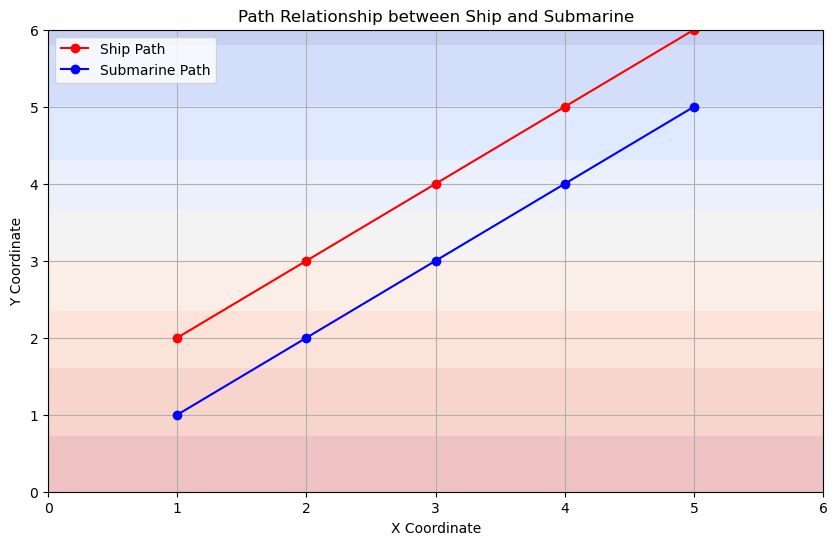
\includegraphics[width=453.55pt,height=295.3pt]{latexImage_90d555ea60b0ee52835daad8231073c5.png}}
\put(56,-371.011){\fontsize{12}{1}\usefont{T1}{cmr}{m}{n}\selectfont\color{color_80434}接}
\put(68,-371.011){\fontsize{12}{1}\usefont{T1}{cmr}{m}{n}\selectfont\color{color_80434}下}
\put(80,-371.011){\fontsize{12}{1}\usefont{T1}{cmr}{m}{n}\selectfont\color{color_80434}来我}
\put(104,-371.011){\fontsize{12}{1}\usefont{T1}{cmr}{m}{n}\selectfont\color{color_80434}们}
\put(116,-371.011){\fontsize{12}{1}\usefont{T1}{cmr}{m}{n}\selectfont\color{color_80434}采}
\put(128,-371.011){\fontsize{12}{1}\usefont{T1}{cmr}{m}{n}\selectfont\color{color_80434}用随机}
\put(164,-371.011){\fontsize{12}{1}\usefont{T1}{cmr}{m}{n}\selectfont\color{color_80434}生}
\put(176,-371.011){\fontsize{12}{1}\usefont{T1}{cmr}{m}{n}\selectfont\color{color_80434}成}
\end{picture}
\begin{tikzpicture}[overlay]
\path(0pt,0pt);
\filldraw[color_277081][even odd rule]
(187.9pt, -373.861pt) -- (239.65pt, -373.861pt)
 -- (239.65pt, -373.861pt)
 -- (239.65pt, -359.911pt)
 -- (239.65pt, -359.911pt)
 -- (187.9pt, -359.911pt) -- cycle
;
\end{tikzpicture}
\begin{picture}(-5,0)(2.5,0)
\put(236,-371.011){\fontsize{12}{1}\usefont{T1}{cmr}{m}{n}\selectfont\color{color_60908} }
\put(188,-371.011){\fontsize{12}{1}\usefont{T1}{cmr}{m}{n}\selectfont\color{color_60908}它将}
\put(212,-371.011){\fontsize{12}{1}\usefont{T1}{cmr}{m}{n}\selectfont\color{color_60908}生}
\put(224,-371.011){\fontsize{12}{1}\usefont{T1}{cmr}{m}{n}\selectfont\color{color_60908}成}
\end{picture}
\begin{tikzpicture}[overlay]
\path(0pt,0pt);
\filldraw[color_277081][even odd rule]
(239.7pt, -373.861pt) -- (266.35pt, -373.861pt)
 -- (266.35pt, -373.861pt)
 -- (266.35pt, -359.911pt)
 -- (266.35pt, -359.911pt)
 -- (239.7pt, -359.911pt) -- cycle
;
\end{tikzpicture}
\begin{picture}(-5,0)(2.5,0)
\put(239.8,-371.011){\fontsize{12}{1}\usefont{T1}{cmr}{m}{n}\selectfont\color{color_60908}1}
\put(247.396,-371.011){\fontsize{12}{1}\usefont{T1}{cmr}{m}{n}\selectfont\color{color_60908}0}
\put(254.992,-371.011){\fontsize{12}{1}\usefont{T1}{cmr}{m}{n}\selectfont\color{color_60908}0}
\put(262.684,-371.011){\fontsize{12}{1}\usefont{T1}{cmr}{m}{n}\selectfont\color{color_60908} }
\end{picture}
\begin{tikzpicture}[overlay]
\path(0pt,0pt);
\filldraw[color_277081][even odd rule]
(266.4pt, -373.861pt) -- (506.35pt, -373.861pt)
 -- (506.35pt, -373.861pt)
 -- (506.35pt, -359.911pt)
 -- (506.35pt, -359.911pt)
 -- (266.4pt, -359.911pt) -- cycle
;
\end{tikzpicture}
\begin{picture}(-5,0)(2.5,0)
\put(266.5,-371.011){\fontsize{12}{1}\usefont{T1}{cmr}{m}{n}\selectfont\color{color_60908}个随机的点数对}
\put(350.5,-371.011){\fontsize{12}{1}\usefont{T1}{cmr}{m}{n}\selectfont\color{color_60908}来}
\put(362.5,-371.011){\fontsize{12}{1}\usefont{T1}{cmr}{m}{n}\selectfont\color{color_60908}模拟主船和潜水的}
\put(458.5,-371.011){\fontsize{12}{1}\usefont{T1}{cmr}{m}{n}\selectfont\color{color_60908}坐}
\put(470.5,-371.011){\fontsize{12}{1}\usefont{T1}{cmr}{m}{n}\selectfont\color{color_60908}标,因}
\end{picture}
\begin{tikzpicture}[overlay]
\path(0pt,0pt);
\filldraw[color_277081][even odd rule]
(55.9pt, -387.861pt) -- (319.85pt, -387.861pt)
 -- (319.85pt, -387.861pt)
 -- (319.85pt, -373.911pt)
 -- (319.85pt, -373.911pt)
 -- (55.9pt, -373.911pt) -- cycle
;
\end{tikzpicture}
\begin{picture}(-5,0)(2.5,0)
\put(56,-385.011){\fontsize{12}{1}\usefont{T1}{cmr}{m}{n}\selectfont\color{color_60908}为}
\put(68,-385.011){\fontsize{12}{1}\usefont{T1}{cmr}{m}{n}\selectfont\color{color_60908}是}
\put(80,-385.011){\fontsize{12}{1}\usefont{T1}{cmr}{m}{n}\selectfont\color{color_60908}模拟数据,}
\put(140,-385.011){\fontsize{12}{1}\usefont{T1}{cmr}{m}{n}\selectfont\color{color_60908}所}
\put(152,-385.011){\fontsize{12}{1}\usefont{T1}{cmr}{m}{n}\selectfont\color{color_60908}以和}
\put(176,-385.011){\fontsize{12}{1}\usefont{T1}{cmr}{m}{n}\selectfont\color{color_60908}实际会}
\put(212,-385.011){\fontsize{12}{1}\usefont{T1}{cmr}{m}{n}\selectfont\color{color_60908}有较}
\put(236,-385.011){\fontsize{12}{1}\usefont{T1}{cmr}{m}{n}\selectfont\color{color_60908}大}
\put(248,-385.011){\fontsize{12}{1}\usefont{T1}{cmr}{m}{n}\selectfont\color{color_60908}偏}
\put(260,-385.011){\fontsize{12}{1}\usefont{T1}{cmr}{m}{n}\selectfont\color{color_60908}差}
\put(272,-385.011){\fontsize{12}{1}\usefont{T1}{cmr}{m}{n}\selectfont\color{color_60908},如下}
\put(308,-385.011){\fontsize{12}{1}\usefont{T1}{cmr}{m}{n}\selectfont\color{color_60908}图}
\put(55.85,-681.611){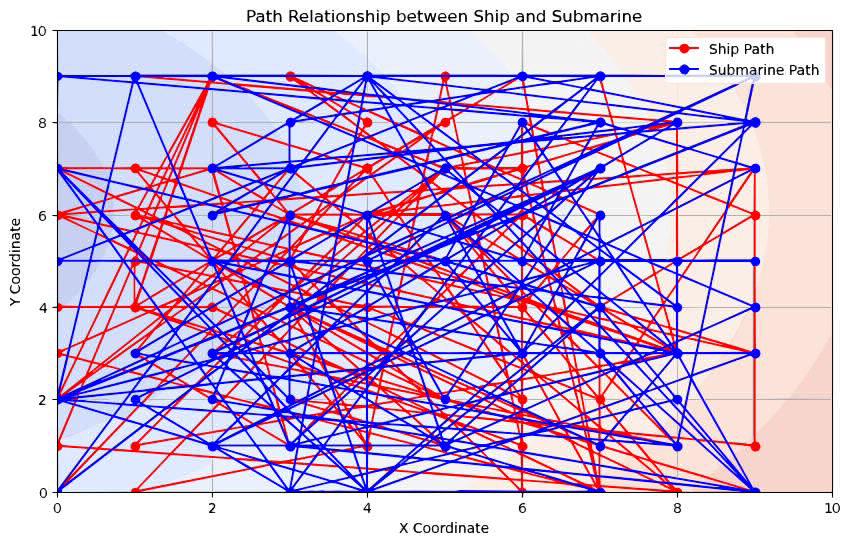
\includegraphics[width=453.55pt,height=290.8pt]{latexImage_7e916b2c457add04a4ba7c54ae330d3f.png}}
\put(56,-712.611){\fontsize{12}{1}\usefont{T1}{cmr}{m}{n}\selectfont\color{color_80434}我}
\put(68,-712.611){\fontsize{12}{1}\usefont{T1}{cmr}{m}{n}\selectfont\color{color_80434}们}
\put(80,-712.611){\fontsize{12}{1}\usefont{T1}{cmr}{m}{n}\selectfont\color{color_80434}接}
\put(92,-712.611){\fontsize{12}{1}\usefont{T1}{cmr}{m}{n}\selectfont\color{color_80434}下}
\put(104,-712.611){\fontsize{12}{1}\usefont{T1}{cmr}{m}{n}\selectfont\color{color_80434}来}
\put(116,-712.611){\fontsize{12}{1}\usefont{T1}{cmr}{m}{n}\selectfont\color{color_80434}根据}
\put(140,-712.611){\fontsize{12}{1}\usefont{T1}{cmr}{m}{n}\selectfont\color{color_80434}坐}
\put(152,-712.611){\fontsize{12}{1}\usefont{T1}{cmr}{m}{n}\selectfont\color{color_80434}标点随机出现的位置进行概率模拟,}
\put(344,-712.611){\fontsize{12}{1}\usefont{T1}{cmr}{m}{n}\selectfont\color{color_80434}继续}
\put(368,-712.611){\fontsize{12}{1}\usefont{T1}{cmr}{m}{n}\selectfont\color{color_80434}使用贝叶斯网络分}
\put(464,-712.611){\fontsize{12}{1}\usefont{T1}{cmr}{m}{n}\selectfont\color{color_80434}类}
\put(476,-712.611){\fontsize{12}{1}\usefont{T1}{cmr}{m}{n}\selectfont\color{color_80434}进行}
\put(56,-726.611){\fontsize{12}{1}\usefont{T1}{cmr}{m}{n}\selectfont\color{color_80434}训}
\put(68,-726.611){\fontsize{12}{1}\usefont{T1}{cmr}{m}{n}\selectfont\color{color_80434}练}
\put(80,-726.611){\fontsize{12}{1}\usefont{T1}{cmr}{m}{n}\selectfont\color{color_80434},}
\put(92,-726.611){\fontsize{12}{1}\usefont{T1}{cmr}{m}{n}\selectfont\color{color_80434}生}
\put(104,-726.611){\fontsize{12}{1}\usefont{T1}{cmr}{m}{n}\selectfont\color{color_80434}成网格预测数据,如下}
\put(224,-726.611){\fontsize{12}{1}\usefont{T1}{cmr}{m}{n}\selectfont\color{color_80434}图}
\end{picture}
\newpage
\begin{tikzpicture}[overlay]\path(0pt,0pt);\end{tikzpicture}
\begin{picture}(-5,0)(2.5,0)
\put(55.85,-199.511){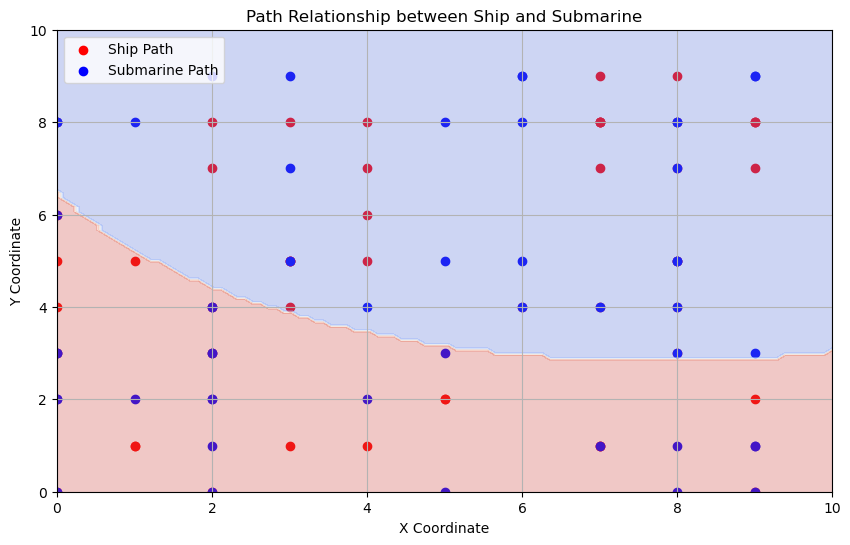
\includegraphics[width=215.25pt,height=138pt]{latexImage_2b90b928288ed4910f626d58d7aa703f.png}}
\put(271.1,-199.511){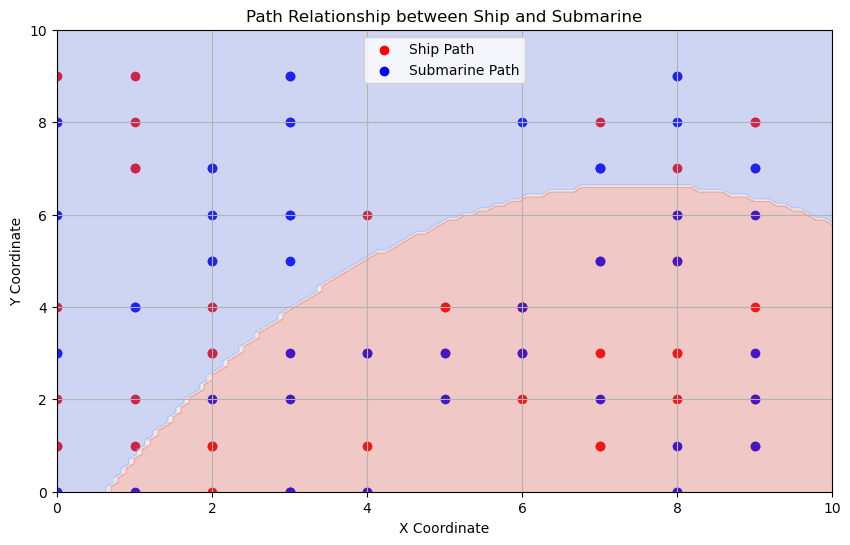
\includegraphics[width=213.75pt,height=137.05pt]{latexImage_c3f5e9413cd90b422ce61daf497ab2da.png}}
\put(55.85,-340.911){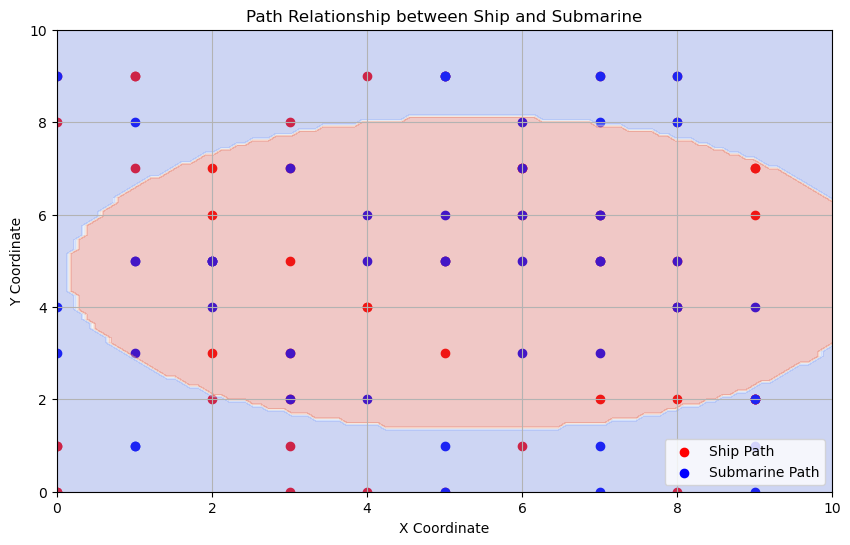
\includegraphics[width=215.1pt,height=137.95pt]{latexImage_18f0475ba80b2f89a92e919ea5f22dd7.png}}
\put(270.95,-340.911){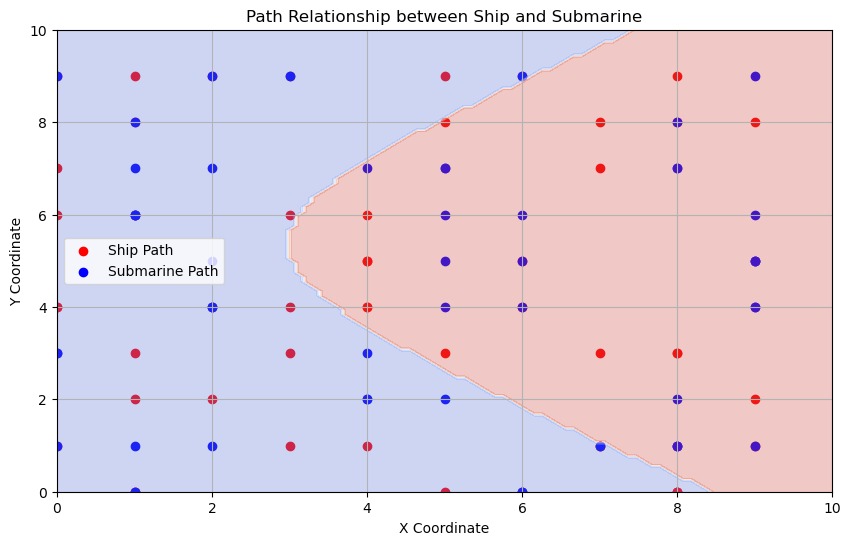
\includegraphics[width=220.5pt,height=141.4pt]{latexImage_98fb3e14983c7942ef339ce8685a41d4.png}}
\put(78,-392.511){\fontsize{16}{1}\usefont{T1}{ptm}{b}{n}\selectfont\color{color_55609}4}
\put(86,-392.511){\fontsize{16}{1}\usefont{T1}{cmr}{m}{n}\selectfont\color{color_55609}、}
\put(119,-392.511){\fontsize{16}{1}\usefont{T1}{cmr}{m}{n}\selectfont\color{color_55609}模型的}
\put(167,-392.511){\fontsize{16}{1}\usefont{T1}{cmr}{m}{n}\selectfont\color{color_55609}误差}
\put(199,-392.511){\fontsize{16}{1}\usefont{T1}{cmr}{m}{n}\selectfont\color{color_55609}分析与改进}
\put(100,-422.511){\fontsize{14}{1}\usefont{T1}{ptm}{b}{n}\selectfont\color{color_55609}a}
\put(106.902,-422.511){\fontsize{14}{1}\usefont{T1}{ptm}{b}{n}\selectfont\color{color_55609})}
\put(116.8,-422.511){\fontsize{14}{1}\usefont{T1}{cmr}{m}{n}\selectfont\color{color_55609}模型分析}
\put(72.8,-451.411){\fontsize{12}{1}\usefont{T1}{cmr}{m}{n}\selectfont\color{color_80434}可以}
\put(96.8,-451.411){\fontsize{12}{1}\usefont{T1}{cmr}{m}{n}\selectfont\color{color_80434}看}
\put(108.8,-451.411){\fontsize{12}{1}\usefont{T1}{cmr}{m}{n}\selectfont\color{color_80434}出主船和潜水器出现的概率分布,因为}
\put(312.8,-451.411){\fontsize{12}{1}\usefont{T1}{cmr}{m}{n}\selectfont\color{color_80434}是}
\put(324.8,-451.411){\fontsize{12}{1}\usefont{T1}{cmr}{m}{n}\selectfont\color{color_80434}模拟数据而且}
\put(396.8,-451.411){\fontsize{12}{1}\usefont{T1}{cmr}{m}{n}\selectfont\color{color_80434}是}
\put(408.8,-451.411){\fontsize{12}{1}\usefont{T1}{cmr}{m}{n}\selectfont\color{color_80434}随机分布,}
\put(468.8,-451.411){\fontsize{12}{1}\usefont{T1}{cmr}{m}{n}\selectfont\color{color_80434}所}
\put(480.8,-451.411){\fontsize{12}{1}\usefont{T1}{cmr}{m}{n}\selectfont\color{color_80434}以}
\put(492.8,-451.411){\fontsize{12}{1}\usefont{T1}{cmr}{m}{n}\selectfont\color{color_80434}造}
\put(72.8,-465.411){\fontsize{12}{1}\usefont{T1}{cmr}{m}{n}\selectfont\color{color_80434}成的}
\put(96.8,-465.411){\fontsize{12}{1}\usefont{T1}{cmr}{m}{n}\selectfont\color{color_80434}偏}
\put(108.8,-465.411){\fontsize{12}{1}\usefont{T1}{cmr}{m}{n}\selectfont\color{color_80434}差是非}
\put(144.8,-465.411){\fontsize{12}{1}\usefont{T1}{cmr}{m}{n}\selectfont\color{color_80434}常}
\put(156.8,-465.411){\fontsize{12}{1}\usefont{T1}{cmr}{m}{n}\selectfont\color{color_80434}大}
\put(168.8,-465.411){\fontsize{12}{1}\usefont{T1}{cmr}{m}{n}\selectfont\color{color_80434}的,不过}
\put(216.8,-465.411){\fontsize{12}{1}\usefont{T1}{cmr}{m}{n}\selectfont\color{color_80434}我}
\put(228.8,-465.411){\fontsize{12}{1}\usefont{T1}{cmr}{m}{n}\selectfont\color{color_80434}们这}
\put(252.8,-465.411){\fontsize{12}{1}\usefont{T1}{cmr}{m}{n}\selectfont\color{color_80434}里}
\put(264.8,-465.411){\fontsize{12}{1}\usefont{T1}{cmr}{m}{n}\selectfont\color{color_80434}讨论的}
\put(300.8,-465.411){\fontsize{12}{1}\usefont{T1}{cmr}{m}{n}\selectfont\color{color_80434}是}
\put(312.8,-465.411){\fontsize{12}{1}\usefont{T1}{cmr}{m}{n}\selectfont\color{color_80434}建立一个合}
\put(372.8,-465.411){\fontsize{12}{1}\usefont{T1}{cmr}{m}{n}\selectfont\color{color_80434}适}
\put(384.8,-465.411){\fontsize{12}{1}\usefont{T1}{cmr}{m}{n}\selectfont\color{color_80434}的模型}
\put(420.8,-465.411){\fontsize{12}{1}\usefont{T1}{cmr}{m}{n}\selectfont\color{color_80434}来}
\put(432.8,-465.411){\fontsize{12}{1}\usefont{T1}{cmr}{m}{n}\selectfont\color{color_80434}推荐设备的}
\put(492.8,-465.411){\fontsize{12}{1}\usefont{T1}{cmr}{m}{n}\selectfont\color{color_80434}初}
\put(72.8,-479.411){\fontsize{12}{1}\usefont{T1}{cmr}{m}{n}\selectfont\color{color_80434}始}
\put(84.8,-479.411){\fontsize{12}{1}\usefont{T1}{cmr}{m}{n}\selectfont\color{color_80434}部署点和搜索模式,以}
\put(204.8,-479.411){\fontsize{12}{1}\usefont{T1}{cmr}{m}{n}\selectfont\color{color_80434}尽}
\put(216.8,-479.411){\fontsize{12}{1}\usefont{T1}{cmr}{m}{n}\selectfont\color{color_80434}量}
\put(228.8,-479.411){\fontsize{12}{1}\usefont{T1}{cmr}{m}{n}\selectfont\color{color_80434}减少}
\put(252.8,-479.411){\fontsize{12}{1}\usefont{T1}{cmr}{m}{n}\selectfont\color{color_80434}丢}
\put(264.8,-479.411){\fontsize{12}{1}\usefont{T1}{cmr}{m}{n}\selectfont\color{color_80434}失潜水器的定位时间,如果}
\put(408.8,-479.411){\fontsize{12}{1}\usefont{T1}{cmr}{m}{n}\selectfont\color{color_80434}我}
\put(420.8,-479.411){\fontsize{12}{1}\usefont{T1}{cmr}{m}{n}\selectfont\color{color_80434}们有}
\put(444.8,-479.411){\fontsize{12}{1}\usefont{T1}{cmr}{m}{n}\selectfont\color{color_80434}历}
\put(456.8,-479.411){\fontsize{12}{1}\usefont{T1}{cmr}{m}{n}\selectfont\color{color_80434}来}
\put(468.8,-479.411){\fontsize{12}{1}\usefont{T1}{cmr}{m}{n}\selectfont\color{color_80434}探险}
\put(492.8,-479.411){\fontsize{12}{1}\usefont{T1}{cmr}{m}{n}\selectfont\color{color_80434}者}
\put(72.8,-493.411){\fontsize{12}{1}\usefont{T1}{cmr}{m}{n}\selectfont\color{color_80434}的}
\put(84.8,-493.411){\fontsize{12}{1}\usefont{T1}{cmr}{m}{n}\selectfont\color{color_80434}航线}
\put(108.8,-493.411){\fontsize{12}{1}\usefont{T1}{cmr}{m}{n}\selectfont\color{color_80434}路}
\put(120.8,-493.411){\fontsize{12}{1}\usefont{T1}{cmr}{m}{n}\selectfont\color{color_80434}线}
\put(132.8,-493.411){\fontsize{12}{1}\usefont{T1}{cmr}{m}{n}\selectfont\color{color_80434},}
\put(144.8,-493.411){\fontsize{12}{1}\usefont{T1}{cmr}{m}{n}\selectfont\color{color_80434}就}
\put(156.8,-493.411){\fontsize{12}{1}\usefont{T1}{cmr}{m}{n}\selectfont\color{color_80434}可以根据}
\put(204.8,-493.411){\fontsize{12}{1}\usefont{T1}{cmr}{m}{n}\selectfont\color{color_80434}航}
\put(216.8,-493.411){\fontsize{12}{1}\usefont{T1}{cmr}{m}{n}\selectfont\color{color_80434}行}
\put(228.8,-493.411){\fontsize{12}{1}\usefont{T1}{cmr}{m}{n}\selectfont\color{color_80434}路}
\put(240.8,-493.411){\fontsize{12}{1}\usefont{T1}{cmr}{m}{n}\selectfont\color{color_80434}线}
\put(252.8,-493.411){\fontsize{12}{1}\usefont{T1}{cmr}{m}{n}\selectfont\color{color_80434}过程中的}
\put(300.8,-493.411){\fontsize{12}{1}\usefont{T1}{cmr}{m}{n}\selectfont\color{color_80434}坐}
\put(312.8,-493.411){\fontsize{12}{1}\usefont{T1}{cmr}{m}{n}\selectfont\color{color_80434}标信息进行多}
\put(384.8,-493.411){\fontsize{12}{1}\usefont{T1}{cmr}{m}{n}\selectfont\color{color_80434}次训}
\put(408.8,-493.411){\fontsize{12}{1}\usefont{T1}{cmr}{m}{n}\selectfont\color{color_80434}练}
\put(420.8,-493.411){\fontsize{12}{1}\usefont{T1}{cmr}{m}{n}\selectfont\color{color_80434},}
\put(432.8,-493.411){\fontsize{12}{1}\usefont{T1}{cmr}{m}{n}\selectfont\color{color_80434}来}
\put(444.8,-493.411){\fontsize{12}{1}\usefont{T1}{cmr}{m}{n}\selectfont\color{color_80434}达}
\put(456.8,-493.411){\fontsize{12}{1}\usefont{T1}{cmr}{m}{n}\selectfont\color{color_80434}到较}
\put(480.8,-493.411){\fontsize{12}{1}\usefont{T1}{cmr}{m}{n}\selectfont\color{color_80434}快}
\put(492.8,-493.411){\fontsize{12}{1}\usefont{T1}{cmr}{m}{n}\selectfont\color{color_80434}搜}
\put(72.8,-507.511){\fontsize{12}{1}\usefont{T1}{cmr}{m}{n}\selectfont\color{color_80434}索到}
\put(96.8,-507.511){\fontsize{12}{1}\usefont{T1}{cmr}{m}{n}\selectfont\color{color_80434}丢}
\put(108.8,-507.511){\fontsize{12}{1}\usefont{T1}{cmr}{m}{n}\selectfont\color{color_80434}失潜水器}
\put(156.8,-507.511){\fontsize{12}{1}\usefont{T1}{ptm}{m}{n}\selectfont\color{color_80434}.}
\put(100,-524.511){\fontsize{12}{1}\usefont{T1}{ptm}{b}{n}\selectfont\color{color_55609}b}
\put(106.684,-524.511){\fontsize{12}{1}\usefont{T1}{ptm}{b}{n}\selectfont\color{color_55609})}
\put(116.8,-524.511){\fontsize{12}{1}\usefont{T1}{cmr}{m}{n}\selectfont\color{color_55609}模型改进与建议}
\put(56,-550.411){\fontsize{11}{1}\usefont{T1}{ptm}{m}{n}\selectfont\color{color_80434} }
\put(58.695,-550.411){\fontsize{11}{1}\usefont{T1}{ptm}{m}{n}\selectfont\color{color_80434} }
\put(61.489,-550.411){\fontsize{11}{1}\usefont{T1}{ptm}{m}{n}\selectfont\color{color_80434} }
\put(64.184,-550.411){\fontsize{11}{1}\usefont{T1}{ptm}{m}{n}\selectfont\color{color_80434} }
\put(66.978,-550.411){\fontsize{11}{1}\usefont{T1}{ptm}{m}{n}\selectfont\color{color_80434} }
\put(69.673,-550.411){\fontsize{11}{1}\usefont{T1}{ptm}{m}{n}\selectfont\color{color_80434} }
\put(72.5,-550.411){\fontsize{11}{1}\usefont{T1}{cmr}{m}{n}\selectfont\color{color_80434}数据集需要}
\put(127.5,-550.411){\fontsize{11}{1}\usefont{T1}{cmr}{m}{n}\selectfont\color{color_80434}采}
\put(138.5,-550.411){\fontsize{11}{1}\usefont{T1}{cmr}{m}{n}\selectfont\color{color_80434}集}
\put(149.5,-550.411){\fontsize{11}{1}\usefont{T1}{cmr}{m}{n}\selectfont\color{color_80434}历}
\put(160.5,-550.411){\fontsize{11}{1}\usefont{T1}{cmr}{m}{n}\selectfont\color{color_80434}年}
\put(171.5,-550.411){\fontsize{11}{1}\usefont{T1}{cmr}{m}{n}\selectfont\color{color_80434}探险}
\put(193.5,-550.411){\fontsize{11}{1}\usefont{T1}{cmr}{m}{n}\selectfont\color{color_80434}者}
\put(204.5,-550.411){\fontsize{11}{1}\usefont{T1}{cmr}{m}{n}\selectfont\color{color_80434}的}
\put(215.5,-550.411){\fontsize{11}{1}\usefont{T1}{cmr}{m}{n}\selectfont\color{color_80434}航}
\put(226.5,-550.411){\fontsize{11}{1}\usefont{T1}{cmr}{m}{n}\selectfont\color{color_80434}行}
\put(237.5,-550.411){\fontsize{11}{1}\usefont{T1}{cmr}{m}{n}\selectfont\color{color_80434}坐}
\put(248.5,-550.411){\fontsize{11}{1}\usefont{T1}{cmr}{m}{n}\selectfont\color{color_80434}标以}
\put(270.5,-550.411){\fontsize{11}{1}\usefont{T1}{cmr}{m}{n}\selectfont\color{color_80434}便}
\put(281.5,-550.411){\fontsize{11}{1}\usefont{T1}{cmr}{m}{n}\selectfont\color{color_80434}于}
\put(292.5,-550.411){\fontsize{11}{1}\usefont{T1}{cmr}{m}{n}\selectfont\color{color_80434}增}
\put(303.5,-550.411){\fontsize{11}{1}\usefont{T1}{cmr}{m}{n}\selectfont\color{color_80434}加置信}
\put(336.5,-550.411){\fontsize{11}{1}\usefont{T1}{cmr}{m}{n}\selectfont\color{color_80434}度}
\put(347.5,-550.411){\fontsize{11}{1}\usefont{T1}{cmr}{m}{n}\selectfont\color{color_80434},不}
\put(369.5,-550.411){\fontsize{11}{1}\usefont{T1}{cmr}{m}{n}\selectfont\color{color_80434}断}
\put(380.5,-550.411){\fontsize{11}{1}\usefont{T1}{cmr}{m}{n}\selectfont\color{color_80434}提}
\put(391.5,-550.411){\fontsize{11}{1}\usefont{T1}{cmr}{m}{n}\selectfont\color{color_80434}取}
\put(402.5,-550.411){\fontsize{11}{1}\usefont{T1}{cmr}{m}{n}\selectfont\color{color_80434}新的}
\put(424.5,-550.411){\fontsize{11}{1}\usefont{T1}{cmr}{m}{n}\selectfont\color{color_80434}特}
\put(435.5,-550.411){\fontsize{11}{1}\usefont{T1}{cmr}{m}{n}\selectfont\color{color_80434}征}
\put(446.5,-550.411){\fontsize{11}{1}\usefont{T1}{cmr}{m}{n}\selectfont\color{color_80434}值}
\put(457.5,-550.411){\fontsize{11}{1}\usefont{T1}{cmr}{m}{n}\selectfont\color{color_80434},比如潜}
\put(56,-563.211){\fontsize{11}{1}\usefont{T1}{cmr}{m}{n}\selectfont\color{color_80434}水器与主船之间的相对}
\put(166,-563.211){\fontsize{11}{1}\usefont{T1}{cmr}{m}{n}\selectfont\color{color_80434}速度}
\put(188,-563.211){\fontsize{11}{1}\usefont{T1}{cmr}{m}{n}\selectfont\color{color_80434},}
\put(199,-563.211){\fontsize{11}{1}\usefont{T1}{cmr}{m}{n}\selectfont\color{color_80434}路}
\put(210,-563.211){\fontsize{11}{1}\usefont{T1}{cmr}{m}{n}\selectfont\color{color_80434}径}
\put(221,-563.211){\fontsize{11}{1}\usefont{T1}{cmr}{m}{n}\selectfont\color{color_80434}曲}
\put(232,-563.211){\fontsize{11}{1}\usefont{T1}{cmr}{m}{n}\selectfont\color{color_80434}率等,使用}
\put(287,-563.211){\fontsize{11}{1}\usefont{T1}{cmr}{m}{n}\selectfont\color{color_80434}交叉}
\put(309,-563.211){\fontsize{11}{1}\usefont{T1}{cmr}{m}{n}\selectfont\color{color_80434}验证找到最优的参数}
\put(408,-563.211){\fontsize{11}{1}\usefont{T1}{cmr}{m}{n}\selectfont\color{color_80434}组}
\put(419,-563.211){\fontsize{11}{1}\usefont{T1}{cmr}{m}{n}\selectfont\color{color_80434}合,比如网格搜索}
\put(507,-563.211){\fontsize{11}{1}\usefont{T1}{cmr}{m}{n}\selectfont\color{color_80434},}
\put(56,-576.011){\fontsize{11}{1}\usefont{T1}{cmr}{m}{n}\selectfont\color{color_80434}随即搜索,贝叶斯优化,}
\put(177,-576.011){\fontsize{11}{1}\usefont{T1}{cmr}{m}{n}\selectfont\color{color_80434}训}
\put(188,-576.011){\fontsize{11}{1}\usefont{T1}{cmr}{m}{n}\selectfont\color{color_80434}练}
\put(199,-576.011){\fontsize{11}{1}\usefont{T1}{cmr}{m}{n}\selectfont\color{color_80434}多}
\put(210,-576.011){\fontsize{11}{1}\usefont{T1}{cmr}{m}{n}\selectfont\color{color_80434}组}
\put(221,-576.011){\fontsize{11}{1}\usefont{T1}{cmr}{m}{n}\selectfont\color{color_80434}模型,对模型进行集成,}
\put(342,-576.011){\fontsize{11}{1}\usefont{T1}{cmr}{m}{n}\selectfont\color{color_80434}降低}
\put(364,-576.011){\fontsize{11}{1}\usefont{T1}{cmr}{m}{n}\selectfont\color{color_80434}方}
\put(375,-576.011){\fontsize{11}{1}\usefont{T1}{cmr}{m}{n}\selectfont\color{color_80434}差}
\put(386,-576.011){\fontsize{11}{1}\usefont{T1}{cmr}{m}{n}\selectfont\color{color_80434},提}
\put(408,-576.011){\fontsize{11}{1}\usefont{T1}{cmr}{m}{n}\selectfont\color{color_80434}升}
\put(419,-576.011){\fontsize{11}{1}\usefont{T1}{cmr}{m}{n}\selectfont\color{color_80434}准确}
\put(441,-576.011){\fontsize{11}{1}\usefont{T1}{cmr}{m}{n}\selectfont\color{color_80434}度}
\put(452,-576.011){\fontsize{11}{1}\usefont{T1}{ptm}{m}{n}\selectfont\color{color_80434}.}
\end{picture}
\newpage
\begin{tikzpicture}[overlay]\path(0pt,0pt);\end{tikzpicture}
\begin{picture}(-5,0)(2.5,0)
\put(105.3,-268.711){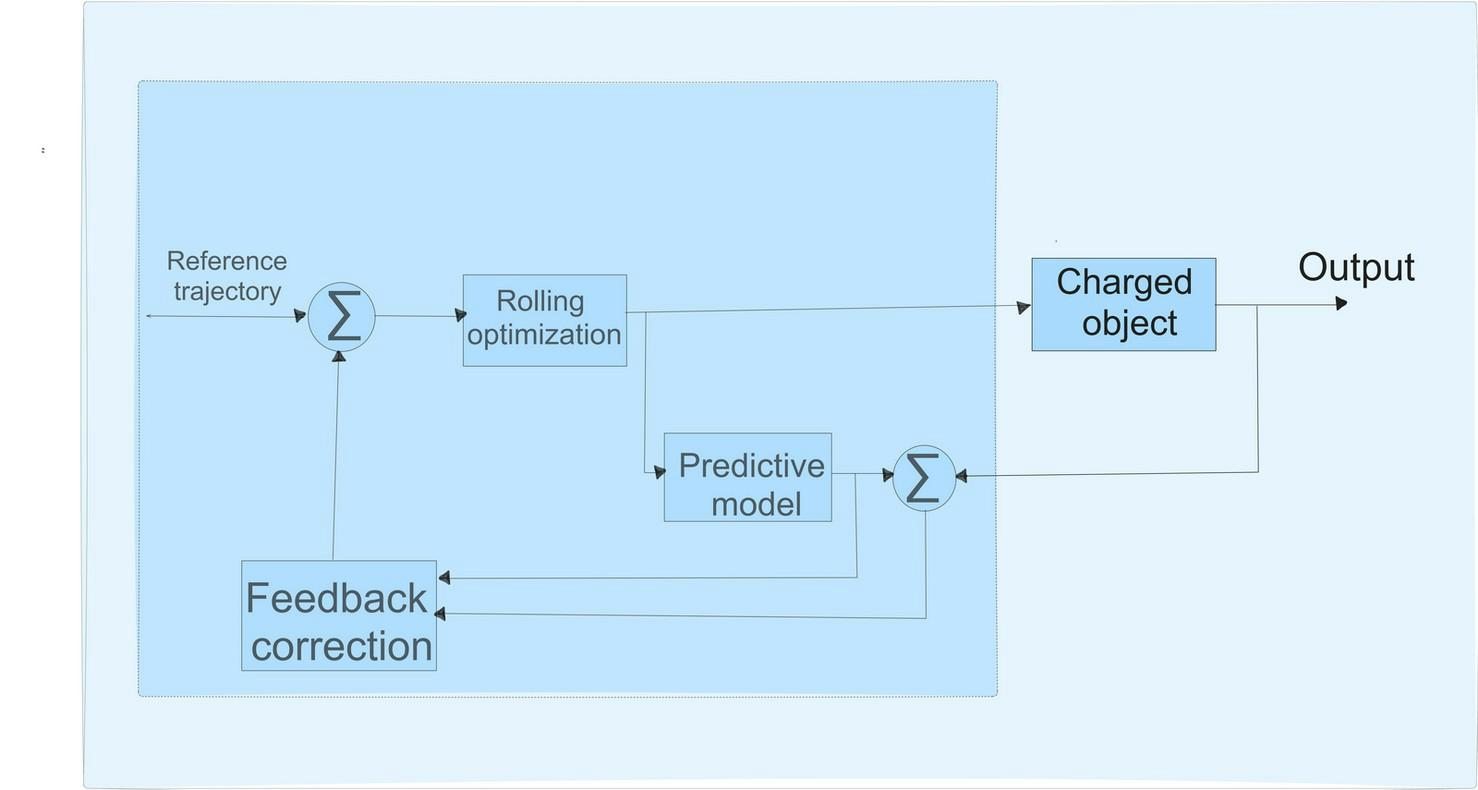
\includegraphics[width=354.75pt,height=207.2pt]{latexImage_9d266c0c553dd44885769b07ec4c122e.png}}
\put(56,-304.111){\fontsize{18}{1}\usefont{T1}{cmr}{m}{n}\selectfont\color{color_55609}七}
\put(74,-304.111){\fontsize{18}{1}\usefont{T1}{cmr}{m}{n}\selectfont\color{color_55609}、}
\put(98,-304.111){\fontsize{18}{1}\usefont{T1}{cmr}{m}{n}\selectfont\color{color_55609}拓}
\put(116,-304.111){\fontsize{18}{1}\usefont{T1}{cmr}{m}{n}\selectfont\color{color_55609}展模型}
\put(78,-338.011){\fontsize{16}{1}\usefont{T1}{ptm}{b}{n}\selectfont\color{color_55609}1}
\put(86,-338.011){\fontsize{16}{1}\usefont{T1}{cmr}{m}{n}\selectfont\color{color_55609}、}
\put(119,-338.011){\fontsize{16}{1}\usefont{T1}{cmr}{m}{n}\selectfont\color{color_55609}问题分析}
\put(56,-368.111){\fontsize{11}{1}\usefont{T1}{cmr}{m}{n}\selectfont\color{color_80434}在这个问题上,}
\put(133,-368.111){\fontsize{11}{1}\usefont{T1}{cmr}{m}{n}\selectfont\color{color_80434}我}
\put(144,-368.111){\fontsize{11}{1}\usefont{T1}{cmr}{m}{n}\selectfont\color{color_80434}们需要将模型}
\put(210,-368.111){\fontsize{11}{1}\usefont{T1}{cmr}{m}{n}\selectfont\color{color_80434}拓}
\put(221,-368.111){\fontsize{11}{1}\usefont{T1}{cmr}{m}{n}\selectfont\color{color_80434}展到}
\put(243,-368.111){\fontsize{11}{1}\usefont{T1}{cmr}{m}{n}\selectfont\color{color_80434}其他}
\put(265,-368.111){\fontsize{11}{1}\usefont{T1}{cmr}{m}{n}\selectfont\color{color_80434}旅游目的地,比如加勒比海等,}
\put(419,-368.111){\fontsize{11}{1}\usefont{T1}{cmr}{m}{n}\selectfont\color{color_80434}也就}
\put(441,-368.111){\fontsize{11}{1}\usefont{T1}{cmr}{m}{n}\selectfont\color{color_80434}是}
\put(452,-368.111){\fontsize{11}{1}\usefont{T1}{cmr}{m}{n}\selectfont\color{color_80434}说}
\put(463,-368.111){\fontsize{11}{1}\usefont{T1}{cmr}{m}{n}\selectfont\color{color_80434}需要将模}
\put(56,-380.911){\fontsize{11}{1}\usefont{T1}{cmr}{m}{n}\selectfont\color{color_80434}型进行环境}
\put(111,-380.911){\fontsize{11}{1}\usefont{T1}{cmr}{m}{n}\selectfont\color{color_80434}迁}
\put(122,-380.911){\fontsize{11}{1}\usefont{T1}{cmr}{m}{n}\selectfont\color{color_80434}移}
\put(133,-380.911){\fontsize{11}{1}\usefont{T1}{cmr}{m}{n}\selectfont\color{color_80434},同时}
\put(166,-380.911){\fontsize{11}{1}\usefont{T1}{cmr}{m}{n}\selectfont\color{color_80434}也}
\put(177,-380.911){\fontsize{11}{1}\usefont{T1}{cmr}{m}{n}\selectfont\color{color_80434}要}
\put(188,-380.911){\fontsize{11}{1}\usefont{T1}{cmr}{m}{n}\selectfont\color{color_80434}考虑}
\put(210,-380.911){\fontsize{11}{1}\usefont{T1}{cmr}{m}{n}\selectfont\color{color_80434}潜水器}
\put(243,-380.911){\fontsize{11}{1}\usefont{T1}{cmr}{m}{n}\selectfont\color{color_80434}运}
\put(254,-380.911){\fontsize{11}{1}\usefont{T1}{cmr}{m}{n}\selectfont\color{color_80434}动模型}
\put(287,-380.911){\fontsize{11}{1}\usefont{T1}{ptm}{m}{n}\selectfont\color{color_80434};}
\put(290,-380.911){\fontsize{11}{1}\usefont{T1}{cmr}{m}{n}\selectfont\color{color_80434}对于存在多个潜水艇的情况,}
\put(433,-380.911){\fontsize{11}{1}\usefont{T1}{cmr}{m}{n}\selectfont\color{color_80434}则}
\put(444,-380.911){\fontsize{11}{1}\usefont{T1}{cmr}{m}{n}\selectfont\color{color_80434}需要使用}
\put(56,-393.811){\fontsize{11}{1}\usefont{T1}{ptm}{m}{n}\selectfont\color{color_80434}M}
\put(65.79,-393.811){\fontsize{11}{1}\usefont{T1}{ptm}{m}{n}\selectfont\color{color_80434}A}
\put(73.688,-393.811){\fontsize{11}{1}\usefont{T1}{ptm}{m}{n}\selectfont\color{color_80434}R}
\put(80.992,-393.811){\fontsize{11}{1}\usefont{T1}{ptm}{m}{n}\selectfont\color{color_80434}L}
\put(90,-393.811){\fontsize{11}{1}\usefont{T1}{cmr}{m}{n}\selectfont\color{color_80434}算法}
\put(112,-393.811){\fontsize{11}{1}\usefont{T1}{cmr}{m}{n}\selectfont\color{color_80434}来}
\put(123,-393.811){\fontsize{11}{1}\usefont{T1}{cmr}{m}{n}\selectfont\color{color_80434}对多个潜水艇}
\put(189,-393.811){\fontsize{11}{1}\usefont{T1}{cmr}{m}{n}\selectfont\color{color_80434}实}
\put(200,-393.811){\fontsize{11}{1}\usefont{T1}{cmr}{m}{n}\selectfont\color{color_80434}现追踪与预测,救}
\put(288,-393.811){\fontsize{11}{1}\usefont{T1}{cmr}{m}{n}\selectfont\color{color_80434}援}
\put(299,-393.811){\fontsize{11}{1}\usefont{T1}{cmr}{m}{n}\selectfont\color{color_80434}首先要}
\put(332,-393.811){\fontsize{11}{1}\usefont{T1}{cmr}{m}{n}\selectfont\color{color_80434}从}
\put(343,-393.811){\fontsize{11}{1}\usefont{T1}{cmr}{m}{n}\selectfont\color{color_80434}概率最}
\put(376,-393.811){\fontsize{11}{1}\usefont{T1}{cmr}{m}{n}\selectfont\color{color_80434}大}
\put(387,-393.811){\fontsize{11}{1}\usefont{T1}{cmr}{m}{n}\selectfont\color{color_80434}的救}
\put(409,-393.811){\fontsize{11}{1}\usefont{T1}{cmr}{m}{n}\selectfont\color{color_80434}援}
\put(420,-393.811){\fontsize{11}{1}\usefont{T1}{cmr}{m}{n}\selectfont\color{color_80434}区域}
\put(442,-393.811){\fontsize{11}{1}\usefont{T1}{cmr}{m}{n}\selectfont\color{color_80434}开始}
\put(464,-393.811){\fontsize{11}{1}\usefont{T1}{cmr}{m}{n}\selectfont\color{color_80434}寻找}
\put(486,-393.811){\fontsize{11}{1}\usefont{T1}{ptm}{m}{n}\selectfont\color{color_80434}.}
\put(78,-414.311){\fontsize{16}{1}\usefont{T1}{ptm}{b}{n}\selectfont\color{color_55609}2}
\put(86,-414.311){\fontsize{16}{1}\usefont{T1}{cmr}{m}{n}\selectfont\color{color_55609}、}
\put(119,-414.311){\fontsize{16}{1}\usefont{T1}{cmr}{m}{n}\selectfont\color{color_55609}模型的准备}
\put(56,-444.311){\fontsize{14}{1}\usefont{T1}{ptm}{b}{n}\selectfont\color{color_55609}a}
\put(62.902,-444.311){\fontsize{14}{1}\usefont{T1}{ptm}{b}{n}\selectfont\color{color_55609})}
\put(67.6,-444.311){\fontsize{14}{1}\usefont{T1}{cmr}{m}{n}\selectfont\color{color_55609}模型}
\put(95.6,-444.311){\fontsize{14}{1}\usefont{T1}{cmr}{m}{n}\selectfont\color{color_55609}假}
\put(109.6,-444.311){\fontsize{14}{1}\usefont{T1}{cmr}{m}{n}\selectfont\color{color_55609}设}
\put(56,-472.311){\fontsize{11}{1}\usefont{T1}{cmr}{m}{n}\selectfont\color{color_80434}}
\put(72.8,-472.311){\fontsize{11}{1}\usefont{T1}{cmr}{m}{n}\selectfont\color{color_80434}假}
\put(83.8,-472.311){\fontsize{11}{1}\usefont{T1}{cmr}{m}{n}\selectfont\color{color_80434}设潜水器与主船}
\put(160.8,-472.311){\fontsize{11}{1}\usefont{T1}{cmr}{m}{n}\selectfont\color{color_80434}所}
\put(171.8,-472.311){\fontsize{11}{1}\usefont{T1}{cmr}{m}{n}\selectfont\color{color_80434}在区域}
\put(204.8,-472.311){\fontsize{11}{1}\usefont{T1}{cmr}{m}{n}\selectfont\color{color_80434}天}
\put(215.8,-472.311){\fontsize{11}{1}\usefont{T1}{cmr}{m}{n}\selectfont\color{color_80434}气等不确定因素}
\put(292.8,-472.311){\fontsize{11}{1}\usefont{T1}{cmr}{m}{n}\selectfont\color{color_80434}忽略}
\put(56,-488.111){\fontsize{11}{1}\usefont{T1}{cmr}{m}{n}\selectfont\color{color_80434}}
\put(72.8,-488.111){\fontsize{11}{1}\usefont{T1}{cmr}{m}{n}\selectfont\color{color_80434}假}
\put(83.8,-488.111){\fontsize{11}{1}\usefont{T1}{cmr}{m}{n}\selectfont\color{color_80434}设多个潜水器的}
\put(160.8,-488.111){\fontsize{11}{1}\usefont{T1}{cmr}{m}{n}\selectfont\color{color_80434}航}
\put(171.8,-488.111){\fontsize{11}{1}\usefont{T1}{cmr}{m}{n}\selectfont\color{color_80434}行}
\put(182.8,-488.111){\fontsize{11}{1}\usefont{T1}{cmr}{m}{n}\selectfont\color{color_80434}路}
\put(193.8,-488.111){\fontsize{11}{1}\usefont{T1}{cmr}{m}{n}\selectfont\color{color_80434}线}
\put(204.8,-488.111){\fontsize{11}{1}\usefont{T1}{cmr}{m}{n}\selectfont\color{color_80434}不}
\put(215.8,-488.111){\fontsize{11}{1}\usefont{T1}{cmr}{m}{n}\selectfont\color{color_80434}互}
\put(226.8,-488.111){\fontsize{11}{1}\usefont{T1}{cmr}{m}{n}\selectfont\color{color_80434}相}
\put(237.8,-488.111){\fontsize{11}{1}\usefont{T1}{cmr}{m}{n}\selectfont\color{color_80434}冲}
\put(248.8,-488.111){\fontsize{11}{1}\usefont{T1}{cmr}{m}{n}\selectfont\color{color_80434}突}
\put(56,-503.911){\fontsize{11}{1}\usefont{T1}{cmr}{m}{n}\selectfont\color{color_80434}}
\put(72.8,-503.911){\fontsize{11}{1}\usefont{T1}{cmr}{m}{n}\selectfont\color{color_80434}假}
\put(83.8,-503.911){\fontsize{11}{1}\usefont{T1}{cmr}{m}{n}\selectfont\color{color_80434}设潜水器的}
\put(138.8,-503.911){\fontsize{11}{1}\usefont{T1}{cmr}{m}{n}\selectfont\color{color_80434}燃料}
\put(160.8,-503.911){\fontsize{11}{1}\usefont{T1}{cmr}{m}{n}\selectfont\color{color_80434}充}
\put(171.8,-503.911){\fontsize{11}{1}\usefont{T1}{cmr}{m}{n}\selectfont\color{color_80434}足}
\put(182.8,-503.911){\fontsize{11}{1}\usefont{T1}{ptm}{m}{n}\selectfont\color{color_80434},}
\put(185.5,-503.911){\fontsize{11}{1}\usefont{T1}{cmr}{m}{n}\selectfont\color{color_80434}通信设备}
\put(229.5,-503.911){\fontsize{11}{1}\usefont{T1}{cmr}{m}{n}\selectfont\color{color_80434}正}
\put(240.5,-503.911){\fontsize{11}{1}\usefont{T1}{cmr}{m}{n}\selectfont\color{color_80434}常}
\put(56,-522.611){\fontsize{14}{1}\usefont{T1}{ptm}{b}{n}\selectfont\color{color_55609}b}
\put(63.7,-522.611){\fontsize{14}{1}\usefont{T1}{ptm}{b}{n}\selectfont\color{color_55609})}
\put(68.4,-522.611){\fontsize{14}{1}\usefont{T1}{cmr}{m}{n}\selectfont\color{color_55609}处}
\put(82.4,-522.611){\fontsize{14}{1}\usefont{T1}{cmr}{m}{n}\selectfont\color{color_55609}理}
\put(96.4,-522.611){\fontsize{14}{1}\usefont{T1}{cmr}{m}{n}\selectfont\color{color_55609}步}
\put(110.4,-522.611){\fontsize{14}{1}\usefont{T1}{cmr}{m}{n}\selectfont\color{color_55609}骤}
\put(56,-550.611){\fontsize{11}{1}\usefont{T1}{cmr}{m}{n}\selectfont\color{color_80434}}
\put(72.8,-550.611){\fontsize{11}{1}\usefont{T1}{cmr}{m}{n}\selectfont\color{color_80434}数据收集与预}
\put(138.8,-550.611){\fontsize{11}{1}\usefont{T1}{cmr}{m}{n}\selectfont\color{color_80434}处}
\put(149.8,-550.611){\fontsize{11}{1}\usefont{T1}{cmr}{m}{n}\selectfont\color{color_80434}理}
\put(72.8,-566.411){\fontsize{11}{1}\usefont{T1}{cmr}{m}{n}\selectfont\color{color_80434}先收集加勒比海地区的主船和潜水器}
\put(248.8,-566.411){\fontsize{11}{1}\usefont{T1}{cmr}{m}{n}\selectfont\color{color_80434}路}
\put(259.8,-566.411){\fontsize{11}{1}\usefont{T1}{cmr}{m}{n}\selectfont\color{color_80434}径}
\put(270.8,-566.411){\fontsize{11}{1}\usefont{T1}{cmr}{m}{n}\selectfont\color{color_80434}数据}
\put(292.8,-566.411){\fontsize{11}{1}\usefont{T1}{ptm}{m}{n}\selectfont\color{color_80434},}
\put(295.5,-566.411){\fontsize{11}{1}\usefont{T1}{cmr}{m}{n}\selectfont\color{color_80434}并进行预}
\put(339.5,-566.411){\fontsize{11}{1}\usefont{T1}{cmr}{m}{n}\selectfont\color{color_80434}处}
\put(350.5,-566.411){\fontsize{11}{1}\usefont{T1}{cmr}{m}{n}\selectfont\color{color_80434}理和}
\put(372.5,-566.411){\fontsize{11}{1}\usefont{T1}{cmr}{m}{n}\selectfont\color{color_80434}清洗}
\put(394.5,-566.411){\fontsize{11}{1}\usefont{T1}{ptm}{m}{n}\selectfont\color{color_80434}.}
\put(56,-582.211){\fontsize{11}{1}\usefont{T1}{cmr}{m}{n}\selectfont\color{color_80434}}
\put(72.8,-582.211){\fontsize{11}{1}\usefont{T1}{cmr}{m}{n}\selectfont\color{color_80434}提}
\put(83.8,-582.211){\fontsize{11}{1}\usefont{T1}{cmr}{m}{n}\selectfont\color{color_80434}取特}
\put(105.8,-582.211){\fontsize{11}{1}\usefont{T1}{cmr}{m}{n}\selectfont\color{color_80434}征}
\put(116.8,-582.211){\fontsize{11}{1}\usefont{T1}{cmr}{m}{n}\selectfont\color{color_80434}值}
\put(72.8,-598.111){\fontsize{11}{1}\usefont{T1}{cmr}{m}{n}\selectfont\color{color_80434}由}
\put(83.8,-598.111){\fontsize{11}{1}\usefont{T1}{cmr}{m}{n}\selectfont\color{color_80434}于需要}
\put(116.8,-598.111){\fontsize{11}{1}\usefont{T1}{cmr}{m}{n}\selectfont\color{color_80434}考虑}
\put(138.8,-598.111){\fontsize{11}{1}\usefont{T1}{cmr}{m}{n}\selectfont\color{color_80434}到海域的变更}
\put(204.8,-598.111){\fontsize{11}{1}\usefont{T1}{ptm}{m}{n}\selectfont\color{color_80434},}
\put(207.5,-598.111){\fontsize{11}{1}\usefont{T1}{cmr}{m}{n}\selectfont\color{color_80434}我}
\put(218.5,-598.111){\fontsize{11}{1}\usefont{T1}{cmr}{m}{n}\selectfont\color{color_80434}们需要加}
\put(262.5,-598.111){\fontsize{11}{1}\usefont{T1}{cmr}{m}{n}\selectfont\color{color_80434}入}
\put(273.5,-598.111){\fontsize{11}{1}\usefont{T1}{cmr}{m}{n}\selectfont\color{color_80434}更多的环境因素}
\put(350.5,-598.111){\fontsize{11}{1}\usefont{T1}{ptm}{m}{n}\selectfont\color{color_80434},}
\put(353.3,-598.111){\fontsize{11}{1}\usefont{T1}{cmr}{m}{n}\selectfont\color{color_80434}比如海底地}
\put(408.3,-598.111){\fontsize{11}{1}\usefont{T1}{cmr}{m}{n}\selectfont\color{color_80434}形}
\put(419.3,-598.111){\fontsize{11}{1}\usefont{T1}{cmr}{m}{n}\selectfont\color{color_80434}的}
\put(430.3,-598.111){\fontsize{11}{1}\usefont{T1}{cmr}{m}{n}\selectfont\color{color_80434}复杂}
\put(452.3,-598.111){\fontsize{11}{1}\usefont{T1}{cmr}{m}{n}\selectfont\color{color_80434}性}
\put(463.3,-598.111){\fontsize{11}{1}\usefont{T1}{ptm}{m}{n}\selectfont\color{color_80434},}
\put(466,-598.111){\fontsize{11}{1}\usefont{T1}{cmr}{m}{n}\selectfont\color{color_80434}海流和}
\put(72.8,-610.911){\fontsize{11}{1}\usefont{T1}{cmr}{m}{n}\selectfont\color{color_80434}风}
\put(83.8,-610.911){\fontsize{11}{1}\usefont{T1}{cmr}{m}{n}\selectfont\color{color_80434}向的}
\put(105.8,-610.911){\fontsize{11}{1}\usefont{T1}{cmr}{m}{n}\selectfont\color{color_80434}影响}
\put(127.8,-610.911){\fontsize{11}{1}\usefont{T1}{ptm}{m}{n}\selectfont\color{color_80434},}
\put(130.5,-610.911){\fontsize{11}{1}\usefont{T1}{cmr}{m}{n}\selectfont\color{color_80434}可能存在的潜水点等}
\put(56,-626.711){\fontsize{11}{1}\usefont{T1}{cmr}{m}{n}\selectfont\color{color_80434}}
\put(72.8,-626.711){\fontsize{11}{1}\usefont{T1}{cmr}{m}{n}\selectfont\color{color_80434}模型的}
\put(105.8,-626.711){\fontsize{11}{1}\usefont{T1}{cmr}{m}{n}\selectfont\color{color_80434}选择}
\put(127.8,-626.711){\fontsize{11}{1}\usefont{T1}{cmr}{m}{n}\selectfont\color{color_80434}和}
\put(138.8,-626.711){\fontsize{11}{1}\usefont{T1}{cmr}{m}{n}\selectfont\color{color_80434}训}
\put(149.8,-626.711){\fontsize{11}{1}\usefont{T1}{cmr}{m}{n}\selectfont\color{color_80434}练}
\put(72.8,-642.611){\fontsize{11}{1}\usefont{T1}{cmr}{m}{n}\selectfont\color{color_80434}针}
\put(83.8,-642.611){\fontsize{11}{1}\usefont{T1}{cmr}{m}{n}\selectfont\color{color_80434}对多个潜水器在同一区域}
\put(204.8,-642.611){\fontsize{11}{1}\usefont{T1}{cmr}{m}{n}\selectfont\color{color_80434}移}
\put(215.8,-642.611){\fontsize{11}{1}\usefont{T1}{cmr}{m}{n}\selectfont\color{color_80434}动的情况}
\put(259.8,-642.611){\fontsize{11}{1}\usefont{T1}{ptm}{m}{n}\selectfont\color{color_80434},}
\put(262.5,-642.611){\fontsize{11}{1}\usefont{T1}{cmr}{m}{n}\selectfont\color{color_80434}一个常用的算法}
\put(339.5,-642.611){\fontsize{11}{1}\usefont{T1}{cmr}{m}{n}\selectfont\color{color_80434}是}
\put(350.5,-642.611){\fontsize{11}{1}\usefont{T1}{cmr}{m}{n}\selectfont\color{color_80434}多}
\put(361.5,-642.611){\fontsize{11}{1}\usefont{T1}{cmr}{m}{n}\selectfont\color{color_80434}智}
\put(372.5,-642.611){\fontsize{11}{1}\usefont{T1}{cmr}{m}{n}\selectfont\color{color_80434}能}
\put(383.5,-642.611){\fontsize{11}{1}\usefont{T1}{cmr}{m}{n}\selectfont\color{color_80434}体}
\put(394.5,-642.611){\fontsize{11}{1}\usefont{T1}{cmr}{m}{n}\selectfont\color{color_80434}强}
\put(405.5,-642.611){\fontsize{11}{1}\usefont{T1}{cmr}{m}{n}\selectfont\color{color_80434}化}
\put(416.5,-642.611){\fontsize{11}{1}\usefont{T1}{cmr}{m}{n}\selectfont\color{color_80434}训}
\put(427.5,-642.611){\fontsize{11}{1}\usefont{T1}{cmr}{m}{n}\selectfont\color{color_80434}练}
\put(438.5,-642.611){\fontsize{11}{1}\usefont{T1}{cmr}{m}{n}\selectfont\color{color_80434}学}
\put(449.5,-642.611){\fontsize{11}{1}\usefont{T1}{cmr}{m}{n}\selectfont\color{color_80434}习}
\put(460.5,-642.611){\fontsize{11}{1}\usefont{T1}{cmr}{m}{n}\selectfont\color{color_80434}中的}
\put(484.7,-642.611){\fontsize{11}{1}\usefont{T1}{ptm}{m}{n}\selectfont\color{color_80434}D}
\put(492.598,-642.611){\fontsize{11}{1}\usefont{T1}{ptm}{m}{n}\selectfont\color{color_80434}e}
\put(497.482,-642.611){\fontsize{11}{1}\usefont{T1}{ptm}{m}{n}\selectfont\color{color_80434}e}
\put(502.366,-642.611){\fontsize{11}{1}\usefont{T1}{ptm}{m}{n}\selectfont\color{color_80434}p}
\put(72.8,-655.411){\fontsize{11}{1}\usefont{T1}{ptm}{m}{n}\selectfont\color{color_80434}-}
\put(76.397,-655.411){\fontsize{11}{1}\usefont{T1}{ptm}{m}{n}\selectfont\color{color_80434}Q}
\put(84.383,-655.411){\fontsize{11}{1}\usefont{T1}{ptm}{m}{n}\selectfont\color{color_80434} }
\put(87.078,-655.411){\fontsize{11}{1}\usefont{T1}{ptm}{m}{n}\selectfont\color{color_80434}-}
\put(90.763,-655.411){\fontsize{11}{1}\usefont{T1}{ptm}{m}{n}\selectfont\color{color_80434}N}
\put(98.661,-655.411){\fontsize{11}{1}\usefont{T1}{ptm}{m}{n}\selectfont\color{color_80434}e}
\put(103.545,-655.411){\fontsize{11}{1}\usefont{T1}{ptm}{m}{n}\selectfont\color{color_80434}t}
\put(106.636,-655.411){\fontsize{11}{1}\usefont{T1}{ptm}{m}{n}\selectfont\color{color_80434}w}
\put(114.534,-655.411){\fontsize{11}{1}\usefont{T1}{ptm}{m}{n}\selectfont\color{color_80434}or}
\put(123.719,-655.411){\fontsize{11}{1}\usefont{T1}{ptm}{m}{n}\selectfont\color{color_80434}k}
\put(131.5,-655.411){\fontsize{11}{1}\usefont{T1}{cmr}{m}{n}\selectfont\color{color_80434}算法}
\put(153.5,-655.411){\fontsize{11}{1}\usefont{T1}{ptm}{m}{n}\selectfont\color{color_80434}(}
\put(157.097,-655.411){\fontsize{11}{1}\usefont{T1}{ptm}{m}{n}\selectfont\color{color_80434}M}
\put(166.887,-655.411){\fontsize{11}{1}\usefont{T1}{ptm}{m}{n}\selectfont\color{color_80434}A}
\put(174.873,-655.411){\fontsize{11}{1}\usefont{T1}{ptm}{m}{n}\selectfont\color{color_80434}D}
\put(182.771,-655.411){\fontsize{11}{1}\usefont{T1}{ptm}{m}{n}\selectfont\color{color_80434}Q}
\put(190.669,-655.411){\fontsize{11}{1}\usefont{T1}{ptm}{m}{n}\selectfont\color{color_80434}N}
\put(198.567,-655.411){\fontsize{11}{1}\usefont{T1}{ptm}{m}{n}\selectfont\color{color_80434})}
\put(202.252,-655.411){\fontsize{11}{1}\usefont{T1}{ptm}{m}{n}\selectfont\color{color_80434},}
\put(205.046,-655.411){\fontsize{11}{1}\usefont{T1}{ptm}{m}{n}\selectfont\color{color_80434}M}
\put(214.836,-655.411){\fontsize{11}{1}\usefont{T1}{ptm}{m}{n}\selectfont\color{color_80434}A}
\put(222.734,-655.411){\fontsize{11}{1}\usefont{T1}{ptm}{m}{n}\selectfont\color{color_80434}D}
\put(230.72,-655.411){\fontsize{11}{1}\usefont{T1}{ptm}{m}{n}\selectfont\color{color_80434}Q}
\put(238.618,-655.411){\fontsize{11}{1}\usefont{T1}{ptm}{m}{n}\selectfont\color{color_80434}N}
\put(248.9,-655.411){\fontsize{11}{1}\usefont{T1}{cmr}{m}{n}\selectfont\color{color_80434}常用于}
\put(281.9,-655.411){\fontsize{11}{1}\usefont{T1}{cmr}{m}{n}\selectfont\color{color_80434}解决}
\put(303.9,-655.411){\fontsize{11}{1}\usefont{T1}{cmr}{m}{n}\selectfont\color{color_80434}多个}
\put(325.9,-655.411){\fontsize{11}{1}\usefont{T1}{cmr}{m}{n}\selectfont\color{color_80434}智}
\put(336.9,-655.411){\fontsize{11}{1}\usefont{T1}{cmr}{m}{n}\selectfont\color{color_80434}能}
\put(347.9,-655.411){\fontsize{11}{1}\usefont{T1}{cmr}{m}{n}\selectfont\color{color_80434}体}
\put(358.9,-655.411){\fontsize{11}{1}\usefont{T1}{cmr}{m}{n}\selectfont\color{color_80434}协}
\put(369.9,-655.411){\fontsize{11}{1}\usefont{T1}{cmr}{m}{n}\selectfont\color{color_80434}作}
\put(380.9,-655.411){\fontsize{11}{1}\usefont{T1}{cmr}{m}{n}\selectfont\color{color_80434}和}
\put(391.9,-655.411){\fontsize{11}{1}\usefont{T1}{cmr}{m}{n}\selectfont\color{color_80434}竞争}
\put(413.9,-655.411){\fontsize{11}{1}\usefont{T1}{cmr}{m}{n}\selectfont\color{color_80434}问题}
\put(56,-671.211){\fontsize{11}{1}\usefont{T1}{cmr}{m}{n}\selectfont\color{color_80434}}
\put(72.8,-671.211){\fontsize{11}{1}\usefont{T1}{cmr}{m}{n}\selectfont\color{color_80434}模型的}
\put(105.8,-671.211){\fontsize{11}{1}\usefont{T1}{cmr}{m}{n}\selectfont\color{color_80434}评估}
\put(127.8,-671.211){\fontsize{11}{1}\usefont{T1}{cmr}{m}{n}\selectfont\color{color_80434}和优化}
\put(72.8,-687.111){\fontsize{11}{1}\usefont{T1}{cmr}{m}{n}\selectfont\color{color_80434}针}
\put(83.8,-687.111){\fontsize{11}{1}\usefont{T1}{cmr}{m}{n}\selectfont\color{color_80434}对加勒比海地区的}
\put(171.8,-687.111){\fontsize{11}{1}\usefont{T1}{cmr}{m}{n}\selectfont\color{color_80434}特殊}
\put(193.8,-687.111){\fontsize{11}{1}\usefont{T1}{cmr}{m}{n}\selectfont\color{color_80434}情况}
\put(215.8,-687.111){\fontsize{11}{1}\usefont{T1}{ptm}{m}{n}\selectfont\color{color_80434},}
\put(218.5,-687.111){\fontsize{11}{1}\usefont{T1}{cmr}{m}{n}\selectfont\color{color_80434}可能要}
\put(251.5,-687.111){\fontsize{11}{1}\usefont{T1}{cmr}{m}{n}\selectfont\color{color_80434}调整}
\put(273.5,-687.111){\fontsize{11}{1}\usefont{T1}{cmr}{m}{n}\selectfont\color{color_80434}模型的}
\put(306.5,-687.111){\fontsize{11}{1}\usefont{T1}{cmr}{m}{n}\selectfont\color{color_80434}超}
\put(317.5,-687.111){\fontsize{11}{1}\usefont{T1}{cmr}{m}{n}\selectfont\color{color_80434}参数}
\put(339.5,-687.111){\fontsize{11}{1}\usefont{T1}{cmr}{m}{n}\selectfont\color{color_80434}或}
\put(350.5,-687.111){\fontsize{11}{1}\usefont{T1}{cmr}{m}{n}\selectfont\color{color_80434}结}
\put(361.5,-687.111){\fontsize{11}{1}\usefont{T1}{cmr}{m}{n}\selectfont\color{color_80434}构}
\put(372.5,-687.111){\fontsize{11}{1}\usefont{T1}{cmr}{m}{n}\selectfont\color{color_80434}以}
\put(383.5,-687.111){\fontsize{11}{1}\usefont{T1}{cmr}{m}{n}\selectfont\color{color_80434}达}
\put(394.5,-687.111){\fontsize{11}{1}\usefont{T1}{cmr}{m}{n}\selectfont\color{color_80434}到更}
\put(416.5,-687.111){\fontsize{11}{1}\usefont{T1}{cmr}{m}{n}\selectfont\color{color_80434}好}
\put(427.5,-687.111){\fontsize{11}{1}\usefont{T1}{cmr}{m}{n}\selectfont\color{color_80434}的性能}
\put(78,-723.311){\fontsize{16}{1}\usefont{T1}{ptm}{b}{n}\selectfont\color{color_55609}3}
\put(86,-723.311){\fontsize{16}{1}\usefont{T1}{cmr}{m}{n}\selectfont\color{color_55609}、}
\put(119,-723.311){\fontsize{16}{1}\usefont{T1}{cmr}{m}{n}\selectfont\color{color_55609}模型的建立}
\put(56,-753.411){\fontsize{11}{1}\usefont{T1}{cmr}{m}{n}\selectfont\color{color_80434}}
\put(72.8,-753.411){\fontsize{11}{1}\usefont{T1}{cmr}{m}{n}\selectfont\color{color_80434}面对上}
\put(105.8,-753.411){\fontsize{11}{1}\usefont{T1}{cmr}{m}{n}\selectfont\color{color_80434}述}
\put(116.8,-753.411){\fontsize{11}{1}\usefont{T1}{cmr}{m}{n}\selectfont\color{color_80434}场}
\put(127.8,-753.411){\fontsize{11}{1}\usefont{T1}{cmr}{m}{n}\selectfont\color{color_80434}景和需}
\put(160.8,-753.411){\fontsize{11}{1}\usefont{T1}{cmr}{m}{n}\selectfont\color{color_80434}求}
\put(171.8,-753.411){\fontsize{11}{1}\usefont{T1}{ptm}{m}{n}\selectfont\color{color_80434},}
\put(174.5,-753.411){\fontsize{11}{1}\usefont{T1}{cmr}{m}{n}\selectfont\color{color_80434}我}
\put(185.5,-753.411){\fontsize{11}{1}\usefont{T1}{cmr}{m}{n}\selectfont\color{color_80434}们}
\put(196.5,-753.411){\fontsize{11}{1}\usefont{T1}{cmr}{m}{n}\selectfont\color{color_80434}决}
\put(207.5,-753.411){\fontsize{11}{1}\usefont{T1}{cmr}{m}{n}\selectfont\color{color_80434}定分}
\put(229.5,-753.411){\fontsize{11}{1}\usefont{T1}{cmr}{m}{n}\selectfont\color{color_80434}别}
\put(240.5,-753.411){\fontsize{11}{1}\usefont{T1}{cmr}{m}{n}\selectfont\color{color_80434}解决}
\put(262.5,-753.411){\fontsize{11}{1}\usefont{T1}{cmr}{m}{n}\selectfont\color{color_80434}地点}
\put(284.5,-753.411){\fontsize{11}{1}\usefont{T1}{cmr}{m}{n}\selectfont\color{color_80434}迁}
\put(295.5,-753.411){\fontsize{11}{1}\usefont{T1}{cmr}{m}{n}\selectfont\color{color_80434}移}
\put(306.5,-753.411){\fontsize{11}{1}\usefont{T1}{cmr}{m}{n}\selectfont\color{color_80434}和}
\put(317.5,-753.411){\fontsize{11}{1}\usefont{T1}{cmr}{m}{n}\selectfont\color{color_80434}多}
\put(328.5,-753.411){\fontsize{11}{1}\usefont{T1}{cmr}{m}{n}\selectfont\color{color_80434}智}
\put(339.5,-753.411){\fontsize{11}{1}\usefont{T1}{cmr}{m}{n}\selectfont\color{color_80434}能}
\put(350.5,-753.411){\fontsize{11}{1}\usefont{T1}{cmr}{m}{n}\selectfont\color{color_80434}体}
\put(361.5,-753.411){\fontsize{11}{1}\usefont{T1}{cmr}{m}{n}\selectfont\color{color_80434}强}
\put(372.5,-753.411){\fontsize{11}{1}\usefont{T1}{cmr}{m}{n}\selectfont\color{color_80434}化学}
\put(394.5,-753.411){\fontsize{11}{1}\usefont{T1}{cmr}{m}{n}\selectfont\color{color_80434}习}
\put(405.5,-753.411){\fontsize{11}{1}\usefont{T1}{cmr}{m}{n}\selectfont\color{color_80434}这}
\put(416.5,-753.411){\fontsize{11}{1}\usefont{T1}{cmr}{m}{n}\selectfont\color{color_80434}两大}
\put(438.5,-753.411){\fontsize{11}{1}\usefont{T1}{cmr}{m}{n}\selectfont\color{color_80434}方向的问题}
\end{picture}
\newpage
\begin{tikzpicture}[overlay]\path(0pt,0pt);\end{tikzpicture}
\begin{picture}(-5,0)(2.5,0)
\put(56,-87.41101){\fontsize{11}{1}\usefont{T1}{cmr}{m}{n}\selectfont\color{color_80434}}
\put(72.8,-87.41101){\fontsize{11}{1}\usefont{T1}{cmr}{m}{n}\selectfont\color{color_80434}地点}
\put(94.8,-87.41101){\fontsize{11}{1}\usefont{T1}{cmr}{m}{n}\selectfont\color{color_80434}迁}
\put(105.8,-87.41101){\fontsize{11}{1}\usefont{T1}{cmr}{m}{n}\selectfont\color{color_80434}移}
\put(72.8,-103.311){\fontsize{11}{1}\usefont{T1}{cmr}{m}{n}\selectfont\color{color_80434}地点}
\put(94.8,-103.311){\fontsize{11}{1}\usefont{T1}{cmr}{m}{n}\selectfont\color{color_80434}迁}
\put(105.8,-103.311){\fontsize{11}{1}\usefont{T1}{cmr}{m}{n}\selectfont\color{color_80434}移会导致}
\put(149.8,-103.311){\fontsize{11}{1}\usefont{T1}{cmr}{m}{n}\selectfont\color{color_80434}主船和潜水器}
\put(215.8,-103.311){\fontsize{11}{1}\usefont{T1}{cmr}{m}{n}\selectfont\color{color_80434}航}
\put(226.8,-103.311){\fontsize{11}{1}\usefont{T1}{cmr}{m}{n}\selectfont\color{color_80434}行过程中的不确定因素}
\put(336.8,-103.311){\fontsize{11}{1}\usefont{T1}{cmr}{m}{n}\selectfont\color{color_80434}增}
\put(347.8,-103.311){\fontsize{11}{1}\usefont{T1}{cmr}{m}{n}\selectfont\color{color_80434}加}
\put(358.8,-103.311){\fontsize{11}{1}\usefont{T1}{ptm}{m}{n}\selectfont\color{color_80434},}
\put(361.5,-103.311){\fontsize{11}{1}\usefont{T1}{cmr}{m}{n}\selectfont\color{color_80434}其}
\put(372.5,-103.311){\fontsize{11}{1}\usefont{T1}{cmr}{m}{n}\selectfont\color{color_80434}中}
\put(383.5,-103.311){\fontsize{11}{1}\usefont{T1}{cmr}{m}{n}\selectfont\color{color_80434}影响}
\put(405.5,-103.311){\fontsize{11}{1}\usefont{T1}{cmr}{m}{n}\selectfont\color{color_80434}最}
\put(416.5,-103.311){\fontsize{11}{1}\usefont{T1}{cmr}{m}{n}\selectfont\color{color_80434}大}
\put(427.5,-103.311){\fontsize{11}{1}\usefont{T1}{cmr}{m}{n}\selectfont\color{color_80434}的因素}
\put(460.5,-103.311){\fontsize{11}{1}\usefont{T1}{cmr}{m}{n}\selectfont\color{color_80434}便是}
\put(482.5,-103.311){\fontsize{11}{1}\usefont{T1}{cmr}{m}{n}\selectfont\color{color_80434}潜水}
\put(72.8,-116.111){\fontsize{11}{1}\usefont{T1}{cmr}{m}{n}\selectfont\color{color_80434}器下潜过程中}
\put(138.8,-116.111){\fontsize{11}{1}\usefont{T1}{cmr}{m}{n}\selectfont\color{color_80434}所}
\put(149.8,-116.111){\fontsize{11}{1}\usefont{T1}{cmr}{m}{n}\selectfont\color{color_80434}到的洋流}
\put(193.8,-116.111){\fontsize{11}{1}\usefont{T1}{cmr}{m}{n}\selectfont\color{color_80434}干扰}
\put(215.8,-116.111){\fontsize{11}{1}\usefont{T1}{ptm}{m}{n}\selectfont\color{color_80434},}
\put(218.5,-116.111){\fontsize{11}{1}\usefont{T1}{cmr}{m}{n}\selectfont\color{color_80434}因此}
\put(240.5,-116.111){\fontsize{11}{1}\usefont{T1}{cmr}{m}{n}\selectfont\color{color_80434}我}
\put(251.5,-116.111){\fontsize{11}{1}\usefont{T1}{cmr}{m}{n}\selectfont\color{color_80434}们在}
\put(273.5,-116.111){\fontsize{11}{1}\usefont{T1}{cmr}{m}{n}\selectfont\color{color_80434}第}
\put(284.5,-116.111){\fontsize{11}{1}\usefont{T1}{cmr}{m}{n}\selectfont\color{color_80434}一问中建立的动力学预测模型将}
\put(438.5,-116.111){\fontsize{11}{1}\usefont{T1}{cmr}{m}{n}\selectfont\color{color_80434}会}
\put(449.5,-116.111){\fontsize{11}{1}\usefont{T1}{cmr}{m}{n}\selectfont\color{color_80434}存在不确定}
\put(72.8,-129.011){\fontsize{11}{1}\usefont{T1}{cmr}{m}{n}\selectfont\color{color_80434}性}
\put(83.8,-129.011){\fontsize{11}{1}\usefont{T1}{ptm}{m}{n}\selectfont\color{color_80434},}
\put(86.5,-129.011){\fontsize{11}{1}\usefont{T1}{cmr}{m}{n}\selectfont\color{color_80434}针}
\put(97.5,-129.011){\fontsize{11}{1}\usefont{T1}{cmr}{m}{n}\selectfont\color{color_80434}对潜水器存在的洋流}
\put(196.5,-129.011){\fontsize{11}{1}\usefont{T1}{cmr}{m}{n}\selectfont\color{color_80434}干扰}
\put(218.5,-129.011){\fontsize{11}{1}\usefont{T1}{ptm}{m}{n}\selectfont\color{color_80434},}
\put(221.3,-129.011){\fontsize{11}{1}\usefont{T1}{cmr}{m}{n}\selectfont\color{color_80434}我}
\put(232.3,-129.011){\fontsize{11}{1}\usefont{T1}{cmr}{m}{n}\selectfont\color{color_80434}们需要建立}
\put(287.3,-129.011){\fontsize{11}{1}\usefont{T1}{cmr}{m}{n}\selectfont\color{color_29791}洋流}
\put(309.3,-129.011){\fontsize{11}{1}\usefont{T1}{cmr}{m}{n}\selectfont\color{color_29791}影响}
\put(331.3,-129.011){\fontsize{11}{1}\usefont{T1}{cmr}{m}{n}\selectfont\color{color_29791}下的潜水器模型}
\put(408.3,-129.011){\fontsize{11}{1}\usefont{T1}{cmr}{m}{n}\selectfont\color{color_80434}以此}
\put(430.3,-129.011){\fontsize{11}{1}\usefont{T1}{cmr}{m}{n}\selectfont\color{color_80434}来}
\put(441.3,-129.011){\fontsize{11}{1}\usefont{T1}{cmr}{m}{n}\selectfont\color{color_80434}提高潜水器的}
\put(72.8,-141.811){\fontsize{11}{1}\usefont{T1}{cmr}{m}{n}\selectfont\color{color_80434}控}
\put(83.8,-141.811){\fontsize{11}{1}\usefont{T1}{cmr}{m}{n}\selectfont\color{color_80434}制性能}
\put(116.8,-141.811){\fontsize{11}{1}\usefont{T1}{ptm}{m}{n}\selectfont\color{color_80434}.}
\put(72.8,-173.311){\fontsize{11}{1}\usefont{T1}{ptm}{m}{n}\selectfont\color{color_80434}a}
\put(77.596,-173.311){\fontsize{11}{1}\usefont{T1}{ptm}{m}{n}\selectfont\color{color_80434})}
\put(81.3,-173.311){\fontsize{11}{1}\usefont{T1}{cmr}{m}{n}\selectfont\color{color_80434}洋流}
\put(103.3,-173.311){\fontsize{11}{1}\usefont{T1}{cmr}{m}{n}\selectfont\color{color_80434}影响}
\put(125.3,-173.311){\fontsize{11}{1}\usefont{T1}{cmr}{m}{n}\selectfont\color{color_80434}下的潜水器模型}
\put(56,-189.211){\fontsize{11}{1}\usefont{T1}{ptm}{m}{n}\selectfont\color{color_80434} }
\put(58.695,-189.211){\fontsize{11}{1}\usefont{T1}{ptm}{m}{n}\selectfont\color{color_80434} }
\put(61.489,-189.211){\fontsize{11}{1}\usefont{T1}{ptm}{m}{n}\selectfont\color{color_80434} }
\put(64.184,-189.211){\fontsize{11}{1}\usefont{T1}{ptm}{m}{n}\selectfont\color{color_80434} }
\put(66.978,-189.211){\fontsize{11}{1}\usefont{T1}{ptm}{m}{n}\selectfont\color{color_80434} }
\put(69.673,-189.211){\fontsize{11}{1}\usefont{T1}{ptm}{m}{n}\selectfont\color{color_80434} }
\put(72.5,-189.211){\fontsize{11}{1}\usefont{T1}{cmr}{m}{n}\selectfont\color{color_80434}假}
\put(83.5,-189.211){\fontsize{11}{1}\usefont{T1}{cmr}{m}{n}\selectfont\color{color_80434}设洋流}
\put(116.5,-189.211){\fontsize{11}{1}\usefont{T1}{cmr}{m}{n}\selectfont\color{color_80434}速度恒}
\put(149.5,-189.211){\fontsize{11}{1}\usefont{T1}{cmr}{m}{n}\selectfont\color{color_80434}定且}
\put(171.5,-189.211){\fontsize{11}{1}\usefont{T1}{cmr}{m}{n}\selectfont\color{color_80434}无旋}
\put(193.5,-189.211){\fontsize{11}{1}\usefont{T1}{ptm}{m}{n}\selectfont\color{color_80434},}
\put(196.2,-189.211){\fontsize{11}{1}\usefont{T1}{cmr}{m}{n}\selectfont\color{color_80434}那}
\put(207.2,-189.211){\fontsize{11}{1}\usefont{T1}{cmr}{m}{n}\selectfont\color{color_80434}我}
\put(218.2,-189.211){\fontsize{11}{1}\usefont{T1}{cmr}{m}{n}\selectfont\color{color_80434}们现在给出以下模型}
\put(317.2,-189.211){\fontsize{11}{1}\usefont{T1}{ptm}{m}{n}\selectfont\color{color_80434}:}
\put(56,-276.511){\fontsize{11}{1}\usefont{T1}{cmr}{m}{n}\selectfont\color{color_80434}其}
\put(67,-276.511){\fontsize{11}{1}\usefont{T1}{cmr}{m}{n}\selectfont\color{color_80434}中}
\put(78,-276.511){\fontsize{11}{1}\usefont{T1}{ptm}{m}{n}\selectfont\color{color_80434},}
\put(173.8,-276.511){\fontsize{11}{1}\usefont{T1}{cmr}{m}{n}\selectfont\color{color_80434}表}
\put(184.8,-276.511){\fontsize{11}{1}\usefont{T1}{cmr}{m}{n}\selectfont\color{color_80434}示}
\put(195.8,-276.511){\fontsize{11}{1}\usefont{T1}{cmr}{m}{n}\selectfont\color{color_80434}机}
\put(206.8,-276.511){\fontsize{11}{1}\usefont{T1}{cmr}{m}{n}\selectfont\color{color_80434}体坐}
\put(228.8,-276.511){\fontsize{11}{1}\usefont{T1}{cmr}{m}{n}\selectfont\color{color_80434}标系下潜水器相对洋流的}
\put(349.8,-276.511){\fontsize{11}{1}\usefont{T1}{cmr}{m}{n}\selectfont\color{color_80434}速度}
\put(371.8,-276.511){\fontsize{11}{1}\usefont{T1}{ptm}{m}{n}\selectfont\color{color_80434},}
\put(464.6,-276.511){\fontsize{11}{1}\usefont{T1}{cmr}{m}{n}\selectfont\color{color_80434}表}
\put(475.6,-276.511){\fontsize{11}{1}\usefont{T1}{cmr}{m}{n}\selectfont\color{color_80434}示}
\put(486.6,-276.511){\fontsize{11}{1}\usefont{T1}{cmr}{m}{n}\selectfont\color{color_80434}在}
\put(497.6,-276.511){\fontsize{11}{1}\usefont{T1}{cmr}{m}{n}\selectfont\color{color_80434}大}
\put(56,-297.911){\fontsize{11}{1}\usefont{T1}{cmr}{m}{n}\selectfont\color{color_80434}地}
\put(67,-297.911){\fontsize{11}{1}\usefont{T1}{cmr}{m}{n}\selectfont\color{color_80434}坐}
\put(78,-297.911){\fontsize{11}{1}\usefont{T1}{cmr}{m}{n}\selectfont\color{color_80434}标系下的洋流}
\put(144,-297.911){\fontsize{11}{1}\usefont{T1}{cmr}{m}{n}\selectfont\color{color_80434}速度}
\put(166,-297.911){\fontsize{11}{1}\usefont{T1}{cmr}{m}{n}\selectfont\color{color_80434}分}
\put(177,-297.911){\fontsize{11}{1}\usefont{T1}{cmr}{m}{n}\selectfont\color{color_80434}量}
\put(188,-297.911){\fontsize{11}{1}\usefont{T1}{ptm}{m}{n}\selectfont\color{color_80434},}
\put(328.8,-297.911){\fontsize{11}{1}\usefont{T1}{cmr}{m}{n}\selectfont\color{color_80434}表}
\put(339.8,-297.911){\fontsize{11}{1}\usefont{T1}{cmr}{m}{n}\selectfont\color{color_80434}示}
\put(350.8,-297.911){\fontsize{11}{1}\usefont{T1}{cmr}{m}{n}\selectfont\color{color_80434}洋流在}
\put(383.8,-297.911){\fontsize{11}{1}\usefont{T1}{cmr}{m}{n}\selectfont\color{color_80434}大}
\put(394.8,-297.911){\fontsize{11}{1}\usefont{T1}{cmr}{m}{n}\selectfont\color{color_80434}地}
\put(405.8,-297.911){\fontsize{11}{1}\usefont{T1}{cmr}{m}{n}\selectfont\color{color_80434}坐}
\put(416.8,-297.911){\fontsize{11}{1}\usefont{T1}{cmr}{m}{n}\selectfont\color{color_80434}标系三个}
\put(460.8,-297.911){\fontsize{11}{1}\usefont{T1}{cmr}{m}{n}\selectfont\color{color_80434}坐}
\put(471.8,-297.911){\fontsize{11}{1}\usefont{T1}{cmr}{m}{n}\selectfont\color{color_80434}标}
\put(482.8,-297.911){\fontsize{11}{1}\usefont{T1}{cmr}{m}{n}\selectfont\color{color_80434}轴}
\put(493.8,-297.911){\fontsize{11}{1}\usefont{T1}{cmr}{m}{n}\selectfont\color{color_80434}上}
\put(56,-318.511){\fontsize{11}{1}\usefont{T1}{cmr}{m}{n}\selectfont\color{color_80434}的}
\put(67,-318.511){\fontsize{11}{1}\usefont{T1}{cmr}{m}{n}\selectfont\color{color_80434}速度}
\put(89,-318.511){\fontsize{11}{1}\usefont{T1}{cmr}{m}{n}\selectfont\color{color_80434}分}
\put(100,-318.511){\fontsize{11}{1}\usefont{T1}{cmr}{m}{n}\selectfont\color{color_80434}量}
\put(111,-318.511){\fontsize{11}{1}\usefont{T1}{ptm}{m}{n}\selectfont\color{color_80434},}
\put(182,-318.511){\fontsize{11}{1}\usefont{T1}{cmr}{m}{n}\selectfont\color{color_80434}表}
\put(193,-318.511){\fontsize{11}{1}\usefont{T1}{cmr}{m}{n}\selectfont\color{color_80434}示刚体惯}
\put(237,-318.511){\fontsize{11}{1}\usefont{T1}{cmr}{m}{n}\selectfont\color{color_80434}性}
\put(248,-318.511){\fontsize{11}{1}\usefont{T1}{cmr}{m}{n}\selectfont\color{color_80434}矩阵}
\put(270,-318.511){\fontsize{11}{1}\usefont{T1}{ptm}{m}{n}\selectfont\color{color_80434},}
\put(338.1,-318.511){\fontsize{11}{1}\usefont{T1}{cmr}{m}{n}\selectfont\color{color_80434}表}
\put(349.1,-318.511){\fontsize{11}{1}\usefont{T1}{cmr}{m}{n}\selectfont\color{color_80434}示刚体}
\put(382.1,-318.511){\fontsize{11}{1}\usefont{T1}{cmr}{m}{n}\selectfont\color{color_80434}向}
\put(393.1,-318.511){\fontsize{11}{1}\usefont{T1}{cmr}{m}{n}\selectfont\color{color_80434}心矩阵}
\put(426.1,-318.511){\fontsize{11}{1}\usefont{T1}{ptm}{m}{n}\selectfont\color{color_80434},}
\put(116,-339.211){\fontsize{11}{1}\usefont{T1}{cmr}{m}{n}\selectfont\color{color_80434}表}
\put(127,-339.211){\fontsize{11}{1}\usefont{T1}{cmr}{m}{n}\selectfont\color{color_80434}示}
\put(138,-339.211){\fontsize{11}{1}\usefont{T1}{cmr}{m}{n}\selectfont\color{color_80434}流}
\put(149,-339.211){\fontsize{11}{1}\usefont{T1}{cmr}{m}{n}\selectfont\color{color_80434}体}
\put(160,-339.211){\fontsize{11}{1}\usefont{T1}{cmr}{m}{n}\selectfont\color{color_80434}向}
\put(171,-339.211){\fontsize{11}{1}\usefont{T1}{cmr}{m}{n}\selectfont\color{color_80434}心矩阵}
\put(204,-339.211){\fontsize{11}{1}\usefont{T1}{ptm}{m}{n}\selectfont\color{color_80434},}
\put(263.1,-339.211){\fontsize{11}{1}\usefont{T1}{cmr}{m}{n}\selectfont\color{color_80434}表}
\put(274.1,-339.211){\fontsize{11}{1}\usefont{T1}{cmr}{m}{n}\selectfont\color{color_80434}示阻}
\put(296.1,-339.211){\fontsize{11}{1}\usefont{T1}{cmr}{m}{n}\selectfont\color{color_80434}尼}
\put(307.1,-339.211){\fontsize{11}{1}\usefont{T1}{cmr}{m}{n}\selectfont\color{color_80434}矩阵}
\put(329.1,-339.211){\fontsize{11}{1}\usefont{T1}{ptm}{m}{n}\selectfont\color{color_80434},}
\put(375.4,-339.211){\fontsize{11}{1}\usefont{T1}{cmr}{m}{n}\selectfont\color{color_80434}表}
\put(386.4,-339.211){\fontsize{11}{1}\usefont{T1}{cmr}{m}{n}\selectfont\color{color_80434}示}
\put(397.4,-339.211){\fontsize{11}{1}\usefont{T1}{cmr}{m}{n}\selectfont\color{color_80434}机}
\put(408.4,-339.211){\fontsize{11}{1}\usefont{T1}{cmr}{m}{n}\selectfont\color{color_80434}体坐}
\put(430.4,-339.211){\fontsize{11}{1}\usefont{T1}{cmr}{m}{n}\selectfont\color{color_80434}标系下重力和}
\put(496.4,-339.211){\fontsize{11}{1}\usefont{T1}{cmr}{m}{n}\selectfont\color{color_80434}浮}
\put(56,-356.811){\fontsize{11}{1}\usefont{T1}{cmr}{m}{n}\selectfont\color{color_80434}力的合力}
\put(100,-356.811){\fontsize{11}{1}\usefont{T1}{ptm}{m}{n}\selectfont\color{color_80434},}
\put(142.5,-356.811){\fontsize{11}{1}\usefont{T1}{cmr}{m}{n}\selectfont\color{color_80434}表}
\put(153.5,-356.811){\fontsize{11}{1}\usefont{T1}{cmr}{m}{n}\selectfont\color{color_80434}示}
\put(164.5,-356.811){\fontsize{11}{1}\usefont{T1}{cmr}{m}{n}\selectfont\color{color_80434}潜水器受到的}
\put(230.5,-356.811){\fontsize{11}{1}\usefont{T1}{cmr}{m}{n}\selectfont\color{color_80434}除}
\put(241.5,-356.811){\fontsize{11}{1}\usefont{T1}{cmr}{m}{n}\selectfont\color{color_80434}洋流}
\put(263.5,-356.811){\fontsize{11}{1}\usefont{T1}{cmr}{m}{n}\selectfont\color{color_80434}干扰}
\put(285.5,-356.811){\fontsize{11}{1}\usefont{T1}{cmr}{m}{n}\selectfont\color{color_80434}外的}
\put(307.5,-356.811){\fontsize{11}{1}\usefont{T1}{cmr}{m}{n}\selectfont\color{color_80434}其他干扰}
\put(351.5,-356.811){\fontsize{11}{1}\usefont{T1}{ptm}{m}{n}\selectfont\color{color_80434},}
\put(354.3,-356.811){\fontsize{11}{1}\usefont{T1}{cmr}{m}{n}\selectfont\color{color_80434}此模型的}
\put(398.3,-356.811){\fontsize{11}{1}\usefont{T1}{cmr}{m}{n}\selectfont\color{color_80434}各}
\put(409.3,-356.811){\fontsize{11}{1}\usefont{T1}{cmr}{m}{n}\selectfont\color{color_80434}个}
\put(420.3,-356.811){\fontsize{11}{1}\usefont{T1}{cmr}{m}{n}\selectfont\color{color_80434}矩阵}
\put(442.3,-356.811){\fontsize{11}{1}\usefont{T1}{cmr}{m}{n}\selectfont\color{color_80434}表}
\put(453.3,-356.811){\fontsize{11}{1}\usefont{T1}{cmr}{m}{n}\selectfont\color{color_80434}达}
\put(464.3,-356.811){\fontsize{11}{1}\usefont{T1}{cmr}{m}{n}\selectfont\color{color_80434}式为}
\put(226.6,-444.911){\fontsize{11}{1}\usefont{T1}{ptm}{m}{n}\selectfont\color{color_80434} }
\put(229.394,-444.911){\fontsize{11}{1}\usefont{T1}{ptm}{m}{n}\selectfont\color{color_80434} }
\put(232.089,-444.911){\fontsize{11}{1}\usefont{T1}{ptm}{m}{n}\selectfont\color{color_80434} }
\put(234.883,-444.911){\fontsize{11}{1}\usefont{T1}{ptm}{m}{n}\selectfont\color{color_80434} }
\put(237.578,-444.911){\fontsize{11}{1}\usefont{T1}{ptm}{m}{n}\selectfont\color{color_80434} }
\put(240.372,-444.911){\fontsize{11}{1}\usefont{T1}{ptm}{m}{n}\selectfont\color{color_80434} }
\put(243.067,-444.911){\fontsize{11}{1}\usefont{T1}{ptm}{m}{n}\selectfont\color{color_80434} }
\put(245.8611,-444.911){\fontsize{11}{1}\usefont{T1}{ptm}{m}{n}\selectfont\color{color_80434} }
\put(248.5561,-444.911){\fontsize{11}{1}\usefont{T1}{ptm}{m}{n}\selectfont\color{color_80434} }
\put(251.3501,-444.911){\fontsize{11}{1}\usefont{T1}{ptm}{m}{n}\selectfont\color{color_80434} }
\put(254.0451,-444.911){\fontsize{11}{1}\usefont{T1}{ptm}{m}{n}\selectfont\color{color_80434} }
\put(346.3,-549.911){\fontsize{11}{1}\usefont{T1}{ptm}{m}{n}\selectfont\color{color_80434} }
\put(348.995,-549.911){\fontsize{11}{1}\usefont{T1}{ptm}{m}{n}\selectfont\color{color_80434} }
\put(351.789,-549.911){\fontsize{11}{1}\usefont{T1}{ptm}{m}{n}\selectfont\color{color_80434} }
\put(224,-681.111){\fontsize{11}{1}\usefont{T1}{ptm}{m}{n}\selectfont\color{color_80434} }
\put(226.794,-681.111){\fontsize{11}{1}\usefont{T1}{ptm}{m}{n}\selectfont\color{color_80434} }
\put(229.489,-681.111){\fontsize{11}{1}\usefont{T1}{ptm}{m}{n}\selectfont\color{color_80434} }
\put(232.283,-681.111){\fontsize{11}{1}\usefont{T1}{ptm}{m}{n}\selectfont\color{color_80434} }
\put(234.978,-681.111){\fontsize{11}{1}\usefont{T1}{ptm}{m}{n}\selectfont\color{color_80434} }
\put(237.772,-681.111){\fontsize{11}{1}\usefont{T1}{ptm}{m}{n}\selectfont\color{color_80434} }
\put(240.467,-681.111){\fontsize{11}{1}\usefont{T1}{ptm}{m}{n}\selectfont\color{color_80434} }
\put(243.261,-681.111){\fontsize{11}{1}\usefont{T1}{ptm}{m}{n}\selectfont\color{color_80434} }
\put(56,-726.711){\fontsize{11}{1}\usefont{T1}{cmr}{m}{n}\selectfont\color{color_29791}其}
\put(67,-726.711){\fontsize{11}{1}\usefont{T1}{cmr}{m}{n}\selectfont\color{color_29791}中,}
\put(89,-726.711){\fontsize{11}{1}\usefont{T1}{ptm}{m}{n}\selectfont\color{color_29791}R}
\put(98.5,-726.711){\fontsize{11}{1}\usefont{T1}{cmr}{m}{n}\selectfont\color{color_29791}为潜水器}
\put(142.5,-726.711){\fontsize{11}{1}\usefont{T1}{cmr}{m}{n}\selectfont\color{color_29791}半径}
\put(164.5,-726.711){\fontsize{11}{1}\usefont{T1}{cmr}{m}{n}\selectfont\color{color_29791},}
\put(175.5,-726.711){\fontsize{11}{1}\usefont{T1}{ptm}{m}{n}\selectfont\color{color_29791}m}
\put(263.3,-726.711){\fontsize{11}{1}\usefont{T1}{cmr}{m}{n}\selectfont\color{color_29791} }
\put(186.3,-726.711){\fontsize{11}{1}\usefont{T1}{cmr}{m}{n}\selectfont\color{color_29791}为潜水器}
\put(230.3,-726.711){\fontsize{11}{1}\usefont{T1}{cmr}{m}{n}\selectfont\color{color_29791}质量}
\put(252.3,-726.711){\fontsize{11}{1}\usefont{T1}{cmr}{m}{n}\selectfont\color{color_29791},}
\put(282.6,-726.711){\fontsize{11}{1}\usefont{T1}{cmr}{m}{n}\selectfont\color{color_29791} }
\put(286.1,-726.711){\fontsize{11}{1}\usefont{T1}{cmr}{m}{n}\selectfont\color{color_29791}为潜水器重}
\put(341.1,-726.711){\fontsize{11}{1}\usefont{T1}{cmr}{m}{n}\selectfont\color{color_29791}心}
\put(352.1,-726.711){\fontsize{11}{1}\usefont{T1}{cmr}{m}{n}\selectfont\color{color_29791}到}
\put(363.1,-726.711){\fontsize{11}{1}\usefont{T1}{cmr}{m}{n}\selectfont\color{color_29791}几}
\put(374.1,-726.711){\fontsize{11}{1}\usefont{T1}{cmr}{m}{n}\selectfont\color{color_29791}何中}
\put(396.1,-726.711){\fontsize{11}{1}\usefont{T1}{cmr}{m}{n}\selectfont\color{color_29791}心}
\put(407.1,-726.711){\fontsize{11}{1}\usefont{T1}{cmr}{m}{n}\selectfont\color{color_29791}的}
\put(418.1,-726.711){\fontsize{11}{1}\usefont{T1}{cmr}{m}{n}\selectfont\color{color_29791}距离}
\put(440.1,-726.711){\fontsize{11}{1}\usefont{T1}{cmr}{m}{n}\selectfont\color{color_29791},}
\put(457.9,-726.711){\fontsize{11}{1}\usefont{T1}{cmr}{m}{n}\selectfont\color{color_29791}为水的}
\put(490.9,-726.711){\fontsize{11}{1}\usefont{T1}{cmr}{m}{n}\selectfont\color{color_29791}密}
\end{picture}
\newpage
\begin{tikzpicture}[overlay]\path(0pt,0pt);\end{tikzpicture}
\begin{picture}(-5,0)(2.5,0)
\put(56,-89.41101){\fontsize{11}{1}\usefont{T1}{cmr}{m}{n}\selectfont\color{color_29791}度}
\put(67,-89.41101){\fontsize{11}{1}\usefont{T1}{cmr}{m}{n}\selectfont\color{color_29791},}
\put(90,-89.41101){\fontsize{11}{1}\usefont{T1}{cmr}{m}{n}\selectfont\color{color_29791} }
\put(93.5,-89.41101){\fontsize{11}{1}\usefont{T1}{cmr}{m}{n}\selectfont\color{color_29791}为潜水器的}
\put(148.5,-89.41101){\fontsize{11}{1}\usefont{T1}{cmr}{m}{n}\selectfont\color{color_29791}平均密度}
\put(192.5,-89.41101){\fontsize{11}{1}\usefont{T1}{cmr}{m}{n}\selectfont\color{color_29791},}
\put(286.6,-89.41101){\fontsize{11}{1}\usefont{T1}{cmr}{m}{n}\selectfont\color{color_29791} }
\put(209.6,-89.41101){\fontsize{11}{1}\usefont{T1}{cmr}{m}{n}\selectfont\color{color_29791}为重力加}
\put(253.6,-89.41101){\fontsize{11}{1}\usefont{T1}{cmr}{m}{n}\selectfont\color{color_29791}速度}
\put(275.6,-89.41101){\fontsize{11}{1}\usefont{T1}{cmr}{m}{n}\selectfont\color{color_29791},}
\put(338.1,-89.41101){\fontsize{11}{1}\usefont{T1}{cmr}{m}{n}\selectfont\color{color_29791}均}
\put(349.1,-89.41101){\fontsize{11}{1}\usefont{T1}{cmr}{m}{n}\selectfont\color{color_29791}为}
\put(360.1,-89.41101){\fontsize{11}{1}\usefont{T1}{cmr}{m}{n}\selectfont\color{color_29791}阻}
\put(371.1,-89.41101){\fontsize{11}{1}\usefont{T1}{cmr}{m}{n}\selectfont\color{color_29791}尼系数,}
\put(495.4,-89.41101){\fontsize{11}{1}\usefont{T1}{cmr}{m}{n}\selectfont\color{color_29791}为}
\put(56,-102.211){\fontsize{11}{1}\usefont{T1}{cmr}{m}{n}\selectfont\color{color_29791}转}
\put(67,-102.211){\fontsize{11}{1}\usefont{T1}{cmr}{m}{n}\selectfont\color{color_29791}动}
\put(78,-102.211){\fontsize{11}{1}\usefont{T1}{cmr}{m}{n}\selectfont\color{color_29791}惯量}
\put(100,-102.211){\fontsize{11}{1}\usefont{T1}{cmr}{m}{n}\selectfont\color{color_29791}。}
\put(56,-133.611){\fontsize{11}{1}\usefont{T1}{cmr}{m}{n}\selectfont\color{color_29791}将受洋流}
\put(100,-133.611){\fontsize{11}{1}\usefont{T1}{cmr}{m}{n}\selectfont\color{color_29791}影响}
\put(122,-133.611){\fontsize{11}{1}\usefont{T1}{cmr}{m}{n}\selectfont\color{color_29791}的潜水器模型}
\put(188,-133.611){\fontsize{11}{1}\usefont{T1}{cmr}{m}{n}\selectfont\color{color_29791}整}
\put(199,-133.611){\fontsize{11}{1}\usefont{T1}{cmr}{m}{n}\selectfont\color{color_29791}理得到如下潜水器动力学模型:}
\put(56,-200.611){\fontsize{11}{1}\usefont{T1}{cmr}{m}{n}\selectfont\color{color_29791}现在}
\put(78,-200.611){\fontsize{11}{1}\usefont{T1}{cmr}{m}{n}\selectfont\color{color_29791}我}
\put(89,-200.611){\fontsize{11}{1}\usefont{T1}{cmr}{m}{n}\selectfont\color{color_29791}们可以确定潜水器}
\put(177,-200.611){\fontsize{11}{1}\usefont{T1}{cmr}{m}{n}\selectfont\color{color_29791}所}
\put(188,-200.611){\fontsize{11}{1}\usefont{T1}{cmr}{m}{n}\selectfont\color{color_29791}受的洋流}
\put(232,-200.611){\fontsize{11}{1}\usefont{T1}{cmr}{m}{n}\selectfont\color{color_29791}干扰}
\put(265.3,-200.611){\fontsize{11}{1}\usefont{T1}{ptm}{m}{n}\selectfont\color{color_29791}:}
\put(56,-282.211){\fontsize{11}{1}\usefont{T1}{cmr}{m}{n}\selectfont\color{color_80434}}
\put(72.8,-282.211){\fontsize{11}{1}\usefont{T1}{cmr}{m}{n}\selectfont\color{color_80434}多}
\put(83.8,-282.211){\fontsize{11}{1}\usefont{T1}{cmr}{m}{n}\selectfont\color{color_80434}智}
\put(94.8,-282.211){\fontsize{11}{1}\usefont{T1}{cmr}{m}{n}\selectfont\color{color_80434}能}
\put(105.8,-282.211){\fontsize{11}{1}\usefont{T1}{cmr}{m}{n}\selectfont\color{color_80434}体}
\put(116.8,-282.211){\fontsize{11}{1}\usefont{T1}{cmr}{m}{n}\selectfont\color{color_80434}强}
\put(127.8,-282.211){\fontsize{11}{1}\usefont{T1}{cmr}{m}{n}\selectfont\color{color_80434}化学}
\put(149.8,-282.211){\fontsize{11}{1}\usefont{T1}{cmr}{m}{n}\selectfont\color{color_80434}习}
\put(160.8,-282.211){\fontsize{11}{1}\usefont{T1}{cmr}{m}{n}\selectfont\color{color_80434}模型}
\put(72.8,-298.011){\fontsize{11}{1}\usefont{T1}{cmr}{m}{n}\selectfont\color{color_80434}我}
\put(83.8,-298.011){\fontsize{11}{1}\usefont{T1}{cmr}{m}{n}\selectfont\color{color_80434}们首先将加勒比海地区的环境建模为一个多}
\put(292.8,-298.011){\fontsize{11}{1}\usefont{T1}{cmr}{m}{n}\selectfont\color{color_80434}智}
\put(303.8,-298.011){\fontsize{11}{1}\usefont{T1}{cmr}{m}{n}\selectfont\color{color_80434}能}
\put(314.8,-298.011){\fontsize{11}{1}\usefont{T1}{cmr}{m}{n}\selectfont\color{color_80434}体}
\put(325.8,-298.011){\fontsize{11}{1}\usefont{T1}{cmr}{m}{n}\selectfont\color{color_80434}环境}
\put(347.8,-298.011){\fontsize{11}{1}\usefont{T1}{ptm}{m}{n}\selectfont\color{color_80434},}
\put(350.5,-298.011){\fontsize{11}{1}\usefont{T1}{cmr}{m}{n}\selectfont\color{color_80434}把}
\put(361.5,-298.011){\fontsize{11}{1}\usefont{T1}{cmr}{m}{n}\selectfont\color{color_80434}每}
\put(372.5,-298.011){\fontsize{11}{1}\usefont{T1}{cmr}{m}{n}\selectfont\color{color_80434}一个潜水器当}
\put(438.5,-298.011){\fontsize{11}{1}\usefont{T1}{cmr}{m}{n}\selectfont\color{color_80434}作}
\put(449.5,-298.011){\fontsize{11}{1}\usefont{T1}{cmr}{m}{n}\selectfont\color{color_80434}一个}
\put(471.5,-298.011){\fontsize{11}{1}\usefont{T1}{cmr}{m}{n}\selectfont\color{color_80434}智}
\put(482.5,-298.011){\fontsize{11}{1}\usefont{T1}{cmr}{m}{n}\selectfont\color{color_80434}能}
\put(493.5,-298.011){\fontsize{11}{1}\usefont{T1}{cmr}{m}{n}\selectfont\color{color_80434}体}
\put(504.5,-298.011){\fontsize{11}{1}\usefont{T1}{ptm}{m}{n}\selectfont\color{color_80434},}
\put(72.8,-310.911){\fontsize{11}{1}\usefont{T1}{cmr}{m}{n}\selectfont\color{color_80434}根据环境}
\put(116.8,-310.911){\fontsize{11}{1}\usefont{T1}{cmr}{m}{n}\selectfont\color{color_80434}状}
\put(127.8,-310.911){\fontsize{11}{1}\usefont{T1}{cmr}{m}{n}\selectfont\color{color_80434}态}
\put(138.8,-310.911){\fontsize{11}{1}\usefont{T1}{cmr}{m}{n}\selectfont\color{color_80434}选择}
\put(160.8,-310.911){\fontsize{11}{1}\usefont{T1}{cmr}{m}{n}\selectfont\color{color_80434}动}
\put(171.8,-310.911){\fontsize{11}{1}\usefont{T1}{cmr}{m}{n}\selectfont\color{color_80434}作}
\put(182.8,-310.911){\fontsize{11}{1}\usefont{T1}{ptm}{m}{n}\selectfont\color{color_80434},}
\put(185.5,-310.911){\fontsize{11}{1}\usefont{T1}{cmr}{m}{n}\selectfont\color{color_80434}并根据}
\put(218.5,-310.911){\fontsize{11}{1}\usefont{T1}{cmr}{m}{n}\selectfont\color{color_80434}奖励}
\put(240.5,-310.911){\fontsize{11}{1}\usefont{T1}{cmr}{m}{n}\selectfont\color{color_80434}信}
\put(251.5,-310.911){\fontsize{11}{1}\usefont{T1}{cmr}{m}{n}\selectfont\color{color_80434}号来调整策略初步}
\put(339.5,-310.911){\fontsize{11}{1}\usefont{T1}{cmr}{m}{n}\selectfont\color{color_80434}确定使用}
\end{picture}
\begin{tikzpicture}[overlay]
\path(0pt,0pt);
\filldraw[color_29791][even odd rule]
(383.4pt, -313.461pt) -- (386.85pt, -313.461pt)
 -- (386.85pt, -313.461pt)
 -- (386.85pt, -300.711pt)
 -- (386.85pt, -300.711pt)
 -- (383.4pt, -300.711pt) -- cycle
;
\end{tikzpicture}
\begin{picture}(-5,0)(2.5,0)
\put(383.5,-310.911){\fontsize{11}{1}\usefont{T1}{cmr}{m}{n}\selectfont\color{color_80434} }
\end{picture}
\begin{tikzpicture}[overlay]
\path(0pt,0pt);
\filldraw[color_29791][even odd rule]
(386.9pt, -313.261pt) -- (463.85pt, -313.261pt)
 -- (463.85pt, -313.261pt)
 -- (463.85pt, -300.611pt)
 -- (463.85pt, -300.611pt)
 -- (386.9pt, -300.611pt) -- cycle
;
\end{tikzpicture}
\begin{picture}(-5,0)(2.5,0)
\put(387,-310.911){\fontsize{11}{1}\usefont{T1}{ptm}{m}{n}\selectfont\color{color_80434}D}
\put(394.898,-310.911){\fontsize{11}{1}\usefont{T1}{ptm}{m}{n}\selectfont\color{color_80434}e}
\put(399.782,-310.911){\fontsize{11}{1}\usefont{T1}{ptm}{m}{n}\selectfont\color{color_80434}e}
\put(404.666,-310.911){\fontsize{11}{1}\usefont{T1}{ptm}{m}{n}\selectfont\color{color_80434}p-}
\put(413.851,-310.911){\fontsize{11}{1}\usefont{T1}{ptm}{m}{n}\selectfont\color{color_80434}Q}
\put(421.749,-310.911){\fontsize{11}{1}\usefont{T1}{ptm}{m}{n}\selectfont\color{color_80434}-}
\put(425.434,-310.911){\fontsize{11}{1}\usefont{T1}{ptm}{m}{n}\selectfont\color{color_80434}N}
\put(433.332,-310.911){\fontsize{11}{1}\usefont{T1}{ptm}{m}{n}\selectfont\color{color_80434}e}
\put(438.216,-310.911){\fontsize{11}{1}\usefont{T1}{ptm}{m}{n}\selectfont\color{color_80434}t}
\put(441.307,-310.911){\fontsize{11}{1}\usefont{T1}{ptm}{m}{n}\selectfont\color{color_80434}w}
\put(449.205,-310.911){\fontsize{11}{1}\usefont{T1}{ptm}{m}{n}\selectfont\color{color_80434}or}
\put(458.39,-310.911){\fontsize{11}{1}\usefont{T1}{ptm}{m}{n}\selectfont\color{color_80434}k}
\end{picture}
\begin{tikzpicture}[overlay]
\path(0pt,0pt);
\filldraw[color_29791][even odd rule]
(463.9pt, -313.261pt) -- (466.05pt, -313.261pt)
 -- (466.05pt, -313.261pt)
 -- (466.05pt, -300.611pt)
 -- (466.05pt, -300.611pt)
 -- (463.9pt, -300.611pt) -- cycle
;
\filldraw[color_29791][even odd rule]
(466.1pt, -313.461pt) -- (499.05pt, -313.461pt)
 -- (499.05pt, -313.461pt)
 -- (499.05pt, -300.711pt)
 -- (499.05pt, -300.711pt)
 -- (466.1pt, -300.711pt) -- cycle
;
\end{tikzpicture}
\begin{picture}(-5,0)(2.5,0)
\put(466.2,-310.911){\fontsize{11}{1}\usefont{T1}{cmr}{m}{n}\selectfont\color{color_80434}算法进}
\end{picture}
\begin{tikzpicture}[overlay]
\path(0pt,0pt);
\filldraw[color_29791][even odd rule]
(72.7pt, -326.261pt) -- (109.15pt, -326.261pt)
 -- (109.15pt, -326.261pt)
 -- (109.15pt, -313.511pt)
 -- (109.15pt, -313.511pt)
 -- (72.7pt, -313.511pt) -- cycle
;
\end{tikzpicture}
\begin{picture}(-5,0)(2.5,0)
\put(105.8,-323.711){\fontsize{11}{1}\usefont{T1}{cmr}{m}{n}\selectfont\color{color_80434} }
\put(72.8,-323.711){\fontsize{11}{1}\usefont{T1}{cmr}{m}{n}\selectfont\color{color_80434}行}
\put(83.8,-323.711){\fontsize{11}{1}\usefont{T1}{cmr}{m}{n}\selectfont\color{color_80434}训}
\put(94.8,-323.711){\fontsize{11}{1}\usefont{T1}{cmr}{m}{n}\selectfont\color{color_80434}练}
\end{picture}
\begin{tikzpicture}[overlay]
\path(0pt,0pt);
\filldraw[color_29791][even odd rule]
(109.2pt, -326.061pt) -- (111.85pt, -326.061pt)
 -- (111.85pt, -326.061pt)
 -- (111.85pt, -313.511pt)
 -- (111.85pt, -313.511pt)
 -- (109.2pt, -313.511pt) -- cycle
;
\end{tikzpicture}
\begin{picture}(-5,0)(2.5,0)
\put(109.3,-323.711){\fontsize{11}{1}\usefont{T1}{ptm}{m}{n}\selectfont\color{color_80434},}
\put(112,-323.711){\fontsize{11}{1}\usefont{T1}{cmr}{m}{n}\selectfont\color{color_84742}通过模拟多个潜水器在环境中}
\put(255,-323.711){\fontsize{11}{1}\usefont{T1}{cmr}{m}{n}\selectfont\color{color_84742}移}
\put(266,-323.711){\fontsize{11}{1}\usefont{T1}{cmr}{m}{n}\selectfont\color{color_84742}动,并根据环境}
\put(343,-323.711){\fontsize{11}{1}\usefont{T1}{cmr}{m}{n}\selectfont\color{color_84742}返回}
\put(365,-323.711){\fontsize{11}{1}\usefont{T1}{cmr}{m}{n}\selectfont\color{color_84742}的}
\put(376,-323.711){\fontsize{11}{1}\usefont{T1}{cmr}{m}{n}\selectfont\color{color_84742}奖励}
\put(398,-323.711){\fontsize{11}{1}\usefont{T1}{cmr}{m}{n}\selectfont\color{color_84742}信}
\put(409,-323.711){\fontsize{11}{1}\usefont{T1}{cmr}{m}{n}\selectfont\color{color_84742}号来训}
\put(442,-323.711){\fontsize{11}{1}\usefont{T1}{cmr}{m}{n}\selectfont\color{color_84742}练智}
\put(464,-323.711){\fontsize{11}{1}\usefont{T1}{cmr}{m}{n}\selectfont\color{color_84742}能}
\put(475,-323.711){\fontsize{11}{1}\usefont{T1}{cmr}{m}{n}\selectfont\color{color_84742}体}
\put(486,-323.711){\fontsize{11}{1}\usefont{T1}{cmr}{m}{n}\selectfont\color{color_84742}的行}
\put(72.8,-336.511){\fontsize{11}{1}\usefont{T1}{cmr}{m}{n}\selectfont\color{color_84742}为}
\put(83.8,-336.511){\fontsize{11}{1}\usefont{T1}{cmr}{m}{n}\selectfont\color{color_84742}.}
\put(197.3,-336.511){\fontsize{11}{1}\usefont{T1}{cmr}{m}{n}\selectfont\color{color_84742} }
\put(87.3,-336.511){\fontsize{11}{1}\usefont{T1}{cmr}{m}{n}\selectfont\color{color_84742}每}
\put(98.3,-336.511){\fontsize{11}{1}\usefont{T1}{cmr}{m}{n}\selectfont\color{color_84742}个}
\put(109.3,-336.511){\fontsize{11}{1}\usefont{T1}{cmr}{m}{n}\selectfont\color{color_84742}智}
\put(120.3,-336.511){\fontsize{11}{1}\usefont{T1}{cmr}{m}{n}\selectfont\color{color_84742}能}
\put(131.3,-336.511){\fontsize{11}{1}\usefont{T1}{cmr}{m}{n}\selectfont\color{color_84742}体都}
\put(153.3,-336.511){\fontsize{11}{1}\usefont{T1}{cmr}{m}{n}\selectfont\color{color_84742}有}
\put(164.3,-336.511){\fontsize{11}{1}\usefont{T1}{cmr}{m}{n}\selectfont\color{color_84742}自己}
\put(186.3,-336.511){\fontsize{11}{1}\usefont{T1}{cmr}{m}{n}\selectfont\color{color_84742}的}
\put(200.8,-336.511){\fontsize{11}{1}\usefont{T1}{cmr}{m}{n}\selectfont\color{color_84742}D}
\put(209.204,-336.511){\fontsize{11}{1}\usefont{T1}{cmr}{m}{n}\selectfont\color{color_84742}Q}
\put(217.894,-336.511){\fontsize{11}{1}\usefont{T1}{cmr}{m}{n}\selectfont\color{color_84742}N}
\put(226.089,-336.511){\fontsize{11}{1}\usefont{T1}{cmr}{m}{n}\selectfont\color{color_84742} }
\put(449.6,-336.511){\fontsize{11}{1}\usefont{T1}{cmr}{m}{n}\selectfont\color{color_84742} }
\put(229.6,-336.511){\fontsize{11}{1}\usefont{T1}{cmr}{m}{n}\selectfont\color{color_84742}模型,并}
\put(273.6,-336.511){\fontsize{11}{1}\usefont{T1}{cmr}{m}{n}\selectfont\color{color_84742}独}
\put(284.6,-336.511){\fontsize{11}{1}\usefont{T1}{cmr}{m}{n}\selectfont\color{color_84742}立地}
\put(306.6,-336.511){\fontsize{11}{1}\usefont{T1}{cmr}{m}{n}\selectfont\color{color_84742}选择}
\put(328.6,-336.511){\fontsize{11}{1}\usefont{T1}{cmr}{m}{n}\selectfont\color{color_84742}动}
\put(339.6,-336.511){\fontsize{11}{1}\usefont{T1}{cmr}{m}{n}\selectfont\color{color_84742}作}
\put(350.6,-336.511){\fontsize{11}{1}\usefont{T1}{cmr}{m}{n}\selectfont\color{color_84742}和学}
\put(372.6,-336.511){\fontsize{11}{1}\usefont{T1}{cmr}{m}{n}\selectfont\color{color_84742}习}
\put(383.6,-336.511){\fontsize{11}{1}\usefont{T1}{cmr}{m}{n}\selectfont\color{color_84742}策略}
\put(405.6,-336.511){\fontsize{11}{1}\usefont{T1}{cmr}{m}{n}\selectfont\color{color_84742}。在}
\put(427.6,-336.511){\fontsize{11}{1}\usefont{T1}{cmr}{m}{n}\selectfont\color{color_84742}每}
\put(438.6,-336.511){\fontsize{11}{1}\usefont{T1}{cmr}{m}{n}\selectfont\color{color_84742}个}
\put(453.1,-336.511){\fontsize{11}{1}\usefont{T1}{cmr}{m}{n}\selectfont\color{color_84742}e}
\put(459.887,-336.511){\fontsize{11}{1}\usefont{T1}{cmr}{m}{n}\selectfont\color{color_84742}p}
\put(466.784,-336.511){\fontsize{11}{1}\usefont{T1}{cmr}{m}{n}\selectfont\color{color_84742}i}
\put(469.875,-336.511){\fontsize{11}{1}\usefont{T1}{cmr}{m}{n}\selectfont\color{color_84742}s}
\put(475.661,-336.511){\fontsize{11}{1}\usefont{T1}{cmr}{m}{n}\selectfont\color{color_84742}o}
\put(482.36,-336.511){\fontsize{11}{1}\usefont{T1}{cmr}{m}{n}\selectfont\color{color_84742}d}
\put(489.345,-336.511){\fontsize{11}{1}\usefont{T1}{cmr}{m}{n}\selectfont\color{color_84742}e}
\put(496.132,-336.511){\fontsize{11}{1}\usefont{T1}{cmr}{m}{n}\selectfont\color{color_84742} }
\put(391.8,-349.311){\fontsize{11}{1}\usefont{T1}{cmr}{m}{n}\selectfont\color{color_84742} }
\put(72.8,-349.311){\fontsize{11}{1}\usefont{T1}{cmr}{m}{n}\selectfont\color{color_84742}中,}
\put(94.8,-349.311){\fontsize{11}{1}\usefont{T1}{cmr}{m}{n}\selectfont\color{color_84742}智}
\put(105.8,-349.311){\fontsize{11}{1}\usefont{T1}{cmr}{m}{n}\selectfont\color{color_84742}能}
\put(116.8,-349.311){\fontsize{11}{1}\usefont{T1}{cmr}{m}{n}\selectfont\color{color_84742}体}
\put(127.8,-349.311){\fontsize{11}{1}\usefont{T1}{cmr}{m}{n}\selectfont\color{color_84742}执}
\put(138.8,-349.311){\fontsize{11}{1}\usefont{T1}{cmr}{m}{n}\selectfont\color{color_84742}行动}
\put(160.8,-349.311){\fontsize{11}{1}\usefont{T1}{cmr}{m}{n}\selectfont\color{color_84742}作}
\put(171.8,-349.311){\fontsize{11}{1}\usefont{T1}{cmr}{m}{n}\selectfont\color{color_84742}并观}
\put(193.8,-349.311){\fontsize{11}{1}\usefont{T1}{cmr}{m}{n}\selectfont\color{color_84742}察}
\put(204.8,-349.311){\fontsize{11}{1}\usefont{T1}{cmr}{m}{n}\selectfont\color{color_84742}环境的}
\put(237.8,-349.311){\fontsize{11}{1}\usefont{T1}{cmr}{m}{n}\selectfont\color{color_84742}反}
\put(248.8,-349.311){\fontsize{11}{1}\usefont{T1}{cmr}{m}{n}\selectfont\color{color_84742}馈}
\put(259.8,-349.311){\fontsize{11}{1}\usefont{T1}{cmr}{m}{n}\selectfont\color{color_84742},}
\put(270.8,-349.311){\fontsize{11}{1}\usefont{T1}{cmr}{m}{n}\selectfont\color{color_84742}然}
\put(281.8,-349.311){\fontsize{11}{1}\usefont{T1}{cmr}{m}{n}\selectfont\color{color_84742}后根据}
\put(314.8,-349.311){\fontsize{11}{1}\usefont{T1}{cmr}{m}{n}\selectfont\color{color_84742}反}
\put(325.8,-349.311){\fontsize{11}{1}\usefont{T1}{cmr}{m}{n}\selectfont\color{color_84742}馈}
\put(336.8,-349.311){\fontsize{11}{1}\usefont{T1}{cmr}{m}{n}\selectfont\color{color_84742}更新}
\put(358.8,-349.311){\fontsize{11}{1}\usefont{T1}{cmr}{m}{n}\selectfont\color{color_84742}自己}
\put(380.8,-349.311){\fontsize{11}{1}\usefont{T1}{cmr}{m}{n}\selectfont\color{color_84742}的}
\put(395.3,-349.311){\fontsize{11}{1}\usefont{T1}{cmr}{m}{n}\selectfont\color{color_84742}Q}
\put(403.902,-349.311){\fontsize{11}{1}\usefont{T1}{cmr}{m}{n}\selectfont\color{color_84742} }
\put(407.4,-349.311){\fontsize{11}{1}\usefont{T1}{cmr}{m}{n}\selectfont\color{color_84742}函数}
\put(193.8,-384.811){\fontsize{11}{1}\usefont{T1}{cmr}{m}{n}\selectfont\color{color_84742}“}
\put(72.8,-384.811){\fontsize{11}{1}\usefont{T1}{cmr}{m}{n}\selectfont\color{color_84742}在}
\put(83.8,-384.811){\fontsize{11}{1}\usefont{T1}{cmr}{m}{n}\selectfont\color{color_84742}强}
\put(94.8,-384.811){\fontsize{11}{1}\usefont{T1}{cmr}{m}{n}\selectfont\color{color_84742}化学}
\put(116.8,-384.811){\fontsize{11}{1}\usefont{T1}{cmr}{m}{n}\selectfont\color{color_84742}习}
\put(127.8,-384.811){\fontsize{11}{1}\usefont{T1}{cmr}{m}{n}\selectfont\color{color_84742}过程中,一个}
\put(199.5,-384.811){\fontsize{11}{1}\usefont{T1}{cmr}{m}{n}\selectfont\color{color_84742}e}
\put(206.199,-384.811){\fontsize{11}{1}\usefont{T1}{cmr}{m}{n}\selectfont\color{color_84742}p}
\put(213.184,-384.811){\fontsize{11}{1}\usefont{T1}{cmr}{m}{n}\selectfont\color{color_84742}i}
\put(216.275,-384.811){\fontsize{11}{1}\usefont{T1}{cmr}{m}{n}\selectfont\color{color_84742}s}
\put(221.973,-384.811){\fontsize{11}{1}\usefont{T1}{cmr}{m}{n}\selectfont\color{color_84742}o}
\put(228.672,-384.811){\fontsize{11}{1}\usefont{T1}{cmr}{m}{n}\selectfont\color{color_84742}d}
\put(235.657,-384.811){\fontsize{11}{1}\usefont{T1}{cmr}{m}{n}\selectfont\color{color_84742}e}
\put(242.444,-384.811){\fontsize{11}{1}\usefont{T1}{cmr}{m}{n}\selectfont\color{color_84742}”}
\put(248.2,-384.811){\fontsize{11}{1}\usefont{T1}{cmr}{m}{n}\selectfont\color{color_84742}通常指的}
\put(292.2,-384.811){\fontsize{11}{1}\usefont{T1}{cmr}{m}{n}\selectfont\color{color_84742}是从}
\put(314.2,-384.811){\fontsize{11}{1}\usefont{T1}{cmr}{m}{n}\selectfont\color{color_84742}环境的}
\put(347.2,-384.811){\fontsize{11}{1}\usefont{T1}{cmr}{m}{n}\selectfont\color{color_84742}初始状}
\put(380.2,-384.811){\fontsize{11}{1}\usefont{T1}{cmr}{m}{n}\selectfont\color{color_84742}态}
\put(391.2,-384.811){\fontsize{11}{1}\usefont{T1}{cmr}{m}{n}\selectfont\color{color_84742}开始}
\put(413.2,-384.811){\fontsize{11}{1}\usefont{T1}{cmr}{m}{n}\selectfont\color{color_84742},}
\put(424.2,-384.811){\fontsize{11}{1}\usefont{T1}{cmr}{m}{n}\selectfont\color{color_84742}直}
\put(435.2,-384.811){\fontsize{11}{1}\usefont{T1}{cmr}{m}{n}\selectfont\color{color_84742}到}
\put(446.2,-384.811){\fontsize{11}{1}\usefont{T1}{cmr}{m}{n}\selectfont\color{color_84742}达}
\put(457.2,-384.811){\fontsize{11}{1}\usefont{T1}{cmr}{m}{n}\selectfont\color{color_84742}到}
\put(468.2,-384.811){\fontsize{11}{1}\usefont{T1}{cmr}{m}{n}\selectfont\color{color_84742}终}
\put(479.2,-384.811){\fontsize{11}{1}\usefont{T1}{cmr}{m}{n}\selectfont\color{color_84742}止}
\put(490.2,-384.811){\fontsize{11}{1}\usefont{T1}{cmr}{m}{n}\selectfont\color{color_84742}状}
\put(105.8,-405.311){\fontsize{11}{1}\usefont{T1}{cmr}{m}{n}\selectfont\color{color_84742}    }
\put(72.8,-405.311){\fontsize{11}{1}\usefont{T1}{cmr}{m}{n}\selectfont\color{color_84742}态为止}
\put(119.792,-405.311){\fontsize{11}{1}\usefont{T1}{cmr}{m}{n}\selectfont\color{color_84742}的一系}
\put(152.8,-405.311){\fontsize{11}{1}\usefont{T1}{cmr}{m}{n}\selectfont\color{color_84742}列}
\put(163.8,-405.311){\fontsize{11}{1}\usefont{T1}{cmr}{m}{n}\selectfont\color{color_84742}动}
\put(174.8,-405.311){\fontsize{11}{1}\usefont{T1}{cmr}{m}{n}\selectfont\color{color_84742}作}
\put(185.8,-405.311){\fontsize{11}{1}\usefont{T1}{cmr}{m}{n}\selectfont\color{color_84742}和}
\put(196.8,-405.311){\fontsize{11}{1}\usefont{T1}{cmr}{m}{n}\selectfont\color{color_84742}状}
\put(207.8,-405.311){\fontsize{11}{1}\usefont{T1}{cmr}{m}{n}\selectfont\color{color_84742}态}
\put(218.8,-405.311){\fontsize{11}{1}\usefont{T1}{cmr}{m}{n}\selectfont\color{color_84742}转}
\put(229.8,-405.311){\fontsize{11}{1}\usefont{T1}{cmr}{m}{n}\selectfont\color{color_84742}换}
\put(240.8,-405.311){\fontsize{11}{1}\usefont{T1}{cmr}{m}{n}\selectfont\color{color_84742}过程}
\put(262.8,-405.311){\fontsize{11}{1}\usefont{T1}{cmr}{m}{n}\selectfont\color{color_84742}.}
\put(266.3,-405.311){\fontsize{11}{1}\usefont{T1}{cmr}{m}{n}\selectfont\color{color_84742}在}
\put(277.3,-405.311){\fontsize{11}{1}\usefont{T1}{cmr}{m}{n}\selectfont\color{color_84742}每}
\put(288.3,-405.311){\fontsize{11}{1}\usefont{T1}{cmr}{m}{n}\selectfont\color{color_84742}个}
\put(301.5,-405.311){\fontsize{11}{1}\usefont{T1}{cmr}{m}{n}\selectfont\color{color_84742}e}
\put(308.199,-405.311){\fontsize{11}{1}\usefont{T1}{cmr}{m}{n}\selectfont\color{color_84742}p}
\put(315.184,-405.311){\fontsize{11}{1}\usefont{T1}{cmr}{m}{n}\selectfont\color{color_84742}i}
\put(318.275,-405.311){\fontsize{11}{1}\usefont{T1}{cmr}{m}{n}\selectfont\color{color_84742}s}
\put(323.973,-405.311){\fontsize{11}{1}\usefont{T1}{cmr}{m}{n}\selectfont\color{color_84742}o}
\put(330.672,-405.311){\fontsize{11}{1}\usefont{T1}{cmr}{m}{n}\selectfont\color{color_84742}d}
\put(337.657,-405.311){\fontsize{11}{1}\usefont{T1}{cmr}{m}{n}\selectfont\color{color_84742}e}
\put(346.7,-405.311){\fontsize{11}{1}\usefont{T1}{cmr}{m}{n}\selectfont\color{color_84742}中,}
\put(368.7,-405.311){\fontsize{11}{1}\usefont{T1}{cmr}{m}{n}\selectfont\color{color_84742}智}
\put(379.7,-405.311){\fontsize{11}{1}\usefont{T1}{cmr}{m}{n}\selectfont\color{color_84742}能}
\put(390.7,-405.311){\fontsize{11}{1}\usefont{T1}{cmr}{m}{n}\selectfont\color{color_84742}体}
\put(401.7,-405.311){\fontsize{11}{1}\usefont{T1}{cmr}{m}{n}\selectfont\color{color_84742}与环境进行}
\put(456.7,-405.311){\fontsize{11}{1}\usefont{T1}{cmr}{m}{n}\selectfont\color{color_84742}交互}
\put(478.7,-405.311){\fontsize{11}{1}\usefont{T1}{cmr}{m}{n}\selectfont\color{color_84742},}
\put(489.7,-405.311){\fontsize{11}{1}\usefont{T1}{cmr}{m}{n}\selectfont\color{color_84742}采}
\put(72.8,-425.811){\fontsize{11}{1}\usefont{T1}{cmr}{m}{n}\selectfont\color{color_84742}取}
\put(83.8,-425.811){\fontsize{11}{1}\usefont{T1}{cmr}{m}{n}\selectfont\color{color_84742}动}
\put(94.8,-425.811){\fontsize{11}{1}\usefont{T1}{cmr}{m}{n}\selectfont\color{color_84742}作}
\put(105.8,-425.811){\fontsize{11}{1}\usefont{T1}{cmr}{m}{n}\selectfont\color{color_84742},观}
\put(127.8,-425.811){\fontsize{11}{1}\usefont{T1}{cmr}{m}{n}\selectfont\color{color_84742}察}
\put(138.8,-425.811){\fontsize{11}{1}\usefont{T1}{cmr}{m}{n}\selectfont\color{color_84742}环境的}
\put(171.8,-425.811){\fontsize{11}{1}\usefont{T1}{cmr}{m}{n}\selectfont\color{color_84742}状}
\put(182.8,-425.811){\fontsize{11}{1}\usefont{T1}{cmr}{m}{n}\selectfont\color{color_84742}态和}
\put(204.8,-425.811){\fontsize{11}{1}\usefont{T1}{cmr}{m}{n}\selectfont\color{color_84742}奖励}
\put(226.8,-425.811){\fontsize{11}{1}\usefont{T1}{cmr}{m}{n}\selectfont\color{color_84742},并}
\put(248.8,-425.811){\fontsize{11}{1}\usefont{T1}{cmr}{m}{n}\selectfont\color{color_84742}尝试}
\put(270.8,-425.811){\fontsize{11}{1}\usefont{T1}{cmr}{m}{n}\selectfont\color{color_84742}通过学}
\put(303.8,-425.811){\fontsize{11}{1}\usefont{T1}{cmr}{m}{n}\selectfont\color{color_84742}习}
\put(314.8,-425.811){\fontsize{11}{1}\usefont{T1}{cmr}{m}{n}\selectfont\color{color_84742}来}
\put(325.8,-425.811){\fontsize{11}{1}\usefont{T1}{cmr}{m}{n}\selectfont\color{color_84742}提高}
\put(347.8,-425.811){\fontsize{11}{1}\usefont{T1}{cmr}{m}{n}\selectfont\color{color_84742}其}
\put(358.8,-425.811){\fontsize{11}{1}\usefont{T1}{cmr}{m}{n}\selectfont\color{color_84742}行为}
\put(380.8,-425.811){\fontsize{11}{1}\usefont{T1}{cmr}{m}{n}\selectfont\color{color_84742}策略}
\put(402.8,-425.811){\fontsize{11}{1}\usefont{T1}{cmr}{m}{n}\selectfont\color{color_84742};}
\put(406.5,-425.811){\fontsize{11}{1}\usefont{T1}{cmr}{m}{n}\selectfont\color{color_84742}在}
\put(417.5,-425.811){\fontsize{11}{1}\usefont{T1}{cmr}{m}{n}\selectfont\color{color_84742}每}
\put(428.5,-425.811){\fontsize{11}{1}\usefont{T1}{cmr}{m}{n}\selectfont\color{color_84742}个}
\put(441.7,-425.811){\fontsize{11}{1}\usefont{T1}{cmr}{m}{n}\selectfont\color{color_84742}e}
\put(448.399,-425.811){\fontsize{11}{1}\usefont{T1}{cmr}{m}{n}\selectfont\color{color_84742}p}
\put(455.384,-425.811){\fontsize{11}{1}\usefont{T1}{cmr}{m}{n}\selectfont\color{color_84742}i}
\put(458.475,-425.811){\fontsize{11}{1}\usefont{T1}{cmr}{m}{n}\selectfont\color{color_84742}s}
\put(464.173,-425.811){\fontsize{11}{1}\usefont{T1}{cmr}{m}{n}\selectfont\color{color_84742}o}
\put(470.872,-425.811){\fontsize{11}{1}\usefont{T1}{cmr}{m}{n}\selectfont\color{color_84742}d}
\put(477.857,-425.811){\fontsize{11}{1}\usefont{T1}{cmr}{m}{n}\selectfont\color{color_84742}e}
\put(486.9,-425.811){\fontsize{11}{1}\usefont{T1}{cmr}{m}{n}\selectfont\color{color_84742}结}
\put(497.9,-425.811){\fontsize{11}{1}\usefont{T1}{cmr}{m}{n}\selectfont\color{color_84742}束}
\put(72.8,-446.311){\fontsize{11}{1}\usefont{T1}{cmr}{m}{n}\selectfont\color{color_84742}时,}
\put(94.8,-446.311){\fontsize{11}{1}\usefont{T1}{cmr}{m}{n}\selectfont\color{color_84742}输}
\put(105.8,-446.311){\fontsize{11}{1}\usefont{T1}{cmr}{m}{n}\selectfont\color{color_84742}出该}
\put(130,-446.311){\fontsize{11}{1}\usefont{T1}{cmr}{m}{n}\selectfont\color{color_84742}e}
\put(136.699,-446.311){\fontsize{11}{1}\usefont{T1}{cmr}{m}{n}\selectfont\color{color_84742}p}
\put(143.684,-446.311){\fontsize{11}{1}\usefont{T1}{cmr}{m}{n}\selectfont\color{color_84742}i}
\put(146.775,-446.311){\fontsize{11}{1}\usefont{T1}{cmr}{m}{n}\selectfont\color{color_84742}s}
\put(152.473,-446.311){\fontsize{11}{1}\usefont{T1}{cmr}{m}{n}\selectfont\color{color_84742}o}
\put(159.172,-446.311){\fontsize{11}{1}\usefont{T1}{cmr}{m}{n}\selectfont\color{color_84742}d}
\put(166.157,-446.311){\fontsize{11}{1}\usefont{T1}{cmr}{m}{n}\selectfont\color{color_84742}e}
\put(175.2,-446.311){\fontsize{11}{1}\usefont{T1}{cmr}{m}{n}\selectfont\color{color_84742}的序}
\put(197.2,-446.311){\fontsize{11}{1}\usefont{T1}{cmr}{m}{n}\selectfont\color{color_84742}号}
\put(208.2,-446.311){\fontsize{11}{1}\usefont{T1}{cmr}{m}{n}\selectfont\color{color_84742}以及}
\put(230.2,-446.311){\fontsize{11}{1}\usefont{T1}{cmr}{m}{n}\selectfont\color{color_84742}智}
\put(241.2,-446.311){\fontsize{11}{1}\usefont{T1}{cmr}{m}{n}\selectfont\color{color_84742}能}
\put(252.2,-446.311){\fontsize{11}{1}\usefont{T1}{cmr}{m}{n}\selectfont\color{color_84742}体}
\put(263.2,-446.311){\fontsize{11}{1}\usefont{T1}{cmr}{m}{n}\selectfont\color{color_84742}在该}
\put(287.4,-446.311){\fontsize{11}{1}\usefont{T1}{cmr}{m}{n}\selectfont\color{color_84742}e}
\put(294.187,-446.311){\fontsize{11}{1}\usefont{T1}{cmr}{m}{n}\selectfont\color{color_84742}p}
\put(301.084,-446.311){\fontsize{11}{1}\usefont{T1}{cmr}{m}{n}\selectfont\color{color_84742}i}
\put(304.175,-446.311){\fontsize{11}{1}\usefont{T1}{cmr}{m}{n}\selectfont\color{color_84742}s}
\put(309.961,-446.311){\fontsize{11}{1}\usefont{T1}{cmr}{m}{n}\selectfont\color{color_84742}o}
\put(316.66,-446.311){\fontsize{11}{1}\usefont{T1}{cmr}{m}{n}\selectfont\color{color_84742}d}
\put(323.645,-446.311){\fontsize{11}{1}\usefont{T1}{cmr}{m}{n}\selectfont\color{color_84742}e}
\put(332.7,-446.311){\fontsize{11}{1}\usefont{T1}{cmr}{m}{n}\selectfont\color{color_84742}中}
\put(343.7,-446.311){\fontsize{11}{1}\usefont{T1}{cmr}{m}{n}\selectfont\color{color_84742}获}
\put(354.7,-446.311){\fontsize{11}{1}\usefont{T1}{cmr}{m}{n}\selectfont\color{color_84742}得的}
\put(376.7,-446.311){\fontsize{11}{1}\usefont{T1}{cmr}{m}{n}\selectfont\color{color_84742}奖励}
\put(398.7,-446.311){\fontsize{11}{1}\usefont{T1}{cmr}{m}{n}\selectfont\color{color_84742}.}
\put(72.65,-649.061){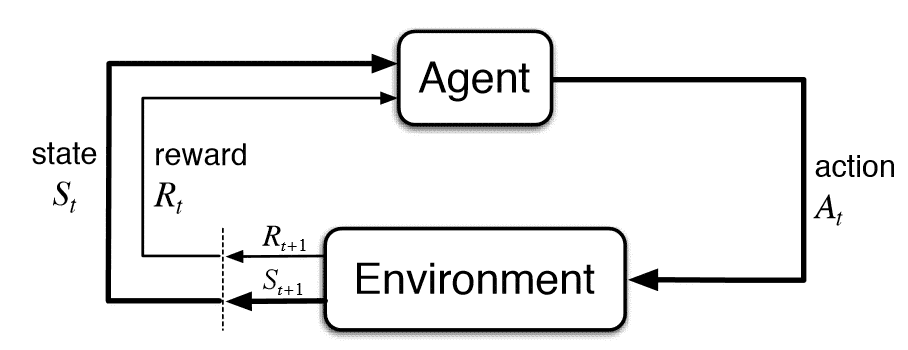
\includegraphics[width=436.75pt,height=168.35pt]{latexImage_b2f218bd62a9bbb6dbcb8a8c902fd537.png}}
\put(72.8,-691.611){\fontsize{11}{1}\usefont{T1}{ptm}{m}{n}\selectfont\color{color_80434}1}
\put(78.201,-691.611){\fontsize{11}{1}\usefont{T1}{ptm}{m}{n}\selectfont\color{color_80434}.}
\put(98,-691.611){\fontsize{12}{1}\usefont{T1}{cmr}{m}{n}\selectfont\color{color_29791}绘}
\put(110,-691.611){\fontsize{12}{1}\usefont{T1}{cmr}{m}{n}\selectfont\color{color_29791}制累}
\put(134,-691.611){\fontsize{12}{1}\usefont{T1}{cmr}{m}{n}\selectfont\color{color_29791}积}
\put(146,-691.611){\fontsize{12}{1}\usefont{T1}{cmr}{m}{n}\selectfont\color{color_29791}奖励曲}
\put(182,-691.611){\fontsize{12}{1}\usefont{T1}{cmr}{m}{n}\selectfont\color{color_29791}线}
\put(194,-691.611){\fontsize{12}{1}\usefont{T1}{cmr}{m}{n}\selectfont\color{color_84742}:在}
\put(218,-691.611){\fontsize{12}{1}\usefont{T1}{cmr}{m}{n}\selectfont\color{color_84742}每}
\put(230,-691.611){\fontsize{12}{1}\usefont{T1}{cmr}{m}{n}\selectfont\color{color_84742}个}
\put(242,-691.611){\fontsize{12}{1}\usefont{T1}{cmr}{m}{n}\selectfont\color{color_84742}训}
\put(254,-691.611){\fontsize{12}{1}\usefont{T1}{cmr}{m}{n}\selectfont\color{color_84742}练}
\put(268.4,-691.611){\fontsize{12}{1}\usefont{T1}{cmr}{m}{n}\selectfont\color{color_84742}e}
\put(275.792,-691.611){\fontsize{12}{1}\usefont{T1}{cmr}{m}{n}\selectfont\color{color_84742}p}
\put(283.388,-691.611){\fontsize{12}{1}\usefont{T1}{cmr}{m}{n}\selectfont\color{color_84742}i}
\put(286.688,-691.611){\fontsize{12}{1}\usefont{T1}{cmr}{m}{n}\selectfont\color{color_84742}s}
\put(292.976,-691.611){\fontsize{12}{1}\usefont{T1}{cmr}{m}{n}\selectfont\color{color_84742}o}
\put(300.272,-691.611){\fontsize{12}{1}\usefont{T1}{cmr}{m}{n}\selectfont\color{color_84742}d}
\put(307.868,-691.611){\fontsize{12}{1}\usefont{T1}{cmr}{m}{n}\selectfont\color{color_84742}e}
\put(317.7,-691.611){\fontsize{12}{1}\usefont{T1}{cmr}{m}{n}\selectfont\color{color_84742}结}
\put(329.7,-691.611){\fontsize{12}{1}\usefont{T1}{cmr}{m}{n}\selectfont\color{color_84742}束}
\put(341.7,-691.611){\fontsize{12}{1}\usefont{T1}{cmr}{m}{n}\selectfont\color{color_84742}时,}
\put(365.7,-691.611){\fontsize{12}{1}\usefont{T1}{cmr}{m}{n}\selectfont\color{color_84742}记录智}
\put(401.7,-691.611){\fontsize{12}{1}\usefont{T1}{cmr}{m}{n}\selectfont\color{color_84742}能}
\put(413.7,-691.611){\fontsize{12}{1}\usefont{T1}{cmr}{m}{n}\selectfont\color{color_84742}体}
\put(425.7,-691.611){\fontsize{12}{1}\usefont{T1}{cmr}{m}{n}\selectfont\color{color_84742}获}
\put(437.7,-691.611){\fontsize{12}{1}\usefont{T1}{cmr}{m}{n}\selectfont\color{color_84742}得的累}
\put(473.7,-691.611){\fontsize{12}{1}\usefont{T1}{cmr}{m}{n}\selectfont\color{color_84742}积}
\put(485.7,-691.611){\fontsize{12}{1}\usefont{T1}{cmr}{m}{n}\selectfont\color{color_84742}奖}
\put(72.8,-712.111){\fontsize{12}{1}\usefont{T1}{cmr}{m}{n}\selectfont\color{color_84742}励}
\put(84.8,-712.111){\fontsize{12}{1}\usefont{T1}{cmr}{m}{n}\selectfont\color{color_84742},并}
\put(108.8,-712.111){\fontsize{12}{1}\usefont{T1}{cmr}{m}{n}\selectfont\color{color_84742}绘}
\put(120.8,-712.111){\fontsize{12}{1}\usefont{T1}{cmr}{m}{n}\selectfont\color{color_84742}制累}
\put(144.8,-712.111){\fontsize{12}{1}\usefont{T1}{cmr}{m}{n}\selectfont\color{color_84742}积}
\put(156.8,-712.111){\fontsize{12}{1}\usefont{T1}{cmr}{m}{n}\selectfont\color{color_84742}奖励}
\put(180.8,-712.111){\fontsize{12}{1}\usefont{T1}{cmr}{m}{n}\selectfont\color{color_84742}随}
\put(192.8,-712.111){\fontsize{12}{1}\usefont{T1}{cmr}{m}{n}\selectfont\color{color_84742}训}
\put(204.8,-712.111){\fontsize{12}{1}\usefont{T1}{cmr}{m}{n}\selectfont\color{color_84742}练轮}
\put(228.8,-712.111){\fontsize{12}{1}\usefont{T1}{cmr}{m}{n}\selectfont\color{color_84742}次}
\put(240.8,-712.111){\fontsize{12}{1}\usefont{T1}{cmr}{m}{n}\selectfont\color{color_84742}变化的}
\put(276.8,-712.111){\fontsize{12}{1}\usefont{T1}{cmr}{m}{n}\selectfont\color{color_84742}曲}
\put(288.8,-712.111){\fontsize{12}{1}\usefont{T1}{cmr}{m}{n}\selectfont\color{color_84742}线图}
\put(312.8,-712.111){\fontsize{12}{1}\usefont{T1}{cmr}{m}{n}\selectfont\color{color_84742}.}
\put(316.6,-712.111){\fontsize{12}{1}\usefont{T1}{cmr}{m}{n}\selectfont\color{color_84742}帮助我}
\put(352.6,-712.111){\fontsize{12}{1}\usefont{T1}{cmr}{m}{n}\selectfont\color{color_84742}们观}
\put(376.6,-712.111){\fontsize{12}{1}\usefont{T1}{cmr}{m}{n}\selectfont\color{color_84742}察智}
\put(400.6,-712.111){\fontsize{12}{1}\usefont{T1}{cmr}{m}{n}\selectfont\color{color_84742}能}
\put(412.6,-712.111){\fontsize{12}{1}\usefont{T1}{cmr}{m}{n}\selectfont\color{color_84742}体}
\put(424.6,-712.111){\fontsize{12}{1}\usefont{T1}{cmr}{m}{n}\selectfont\color{color_84742}在}
\put(436.6,-712.111){\fontsize{12}{1}\usefont{T1}{cmr}{m}{n}\selectfont\color{color_84742}训}
\put(448.6,-712.111){\fontsize{12}{1}\usefont{T1}{cmr}{m}{n}\selectfont\color{color_84742}练}
\put(460.6,-712.111){\fontsize{12}{1}\usefont{T1}{cmr}{m}{n}\selectfont\color{color_84742}过程中}
\put(496.6,-712.111){\fontsize{12}{1}\usefont{T1}{cmr}{m}{n}\selectfont\color{color_84742}奖}
\put(72.8,-732.611){\fontsize{12}{1}\usefont{T1}{cmr}{m}{n}\selectfont\color{color_84742}励}
\put(84.8,-732.611){\fontsize{12}{1}\usefont{T1}{cmr}{m}{n}\selectfont\color{color_84742}的变化}
\put(120.8,-732.611){\fontsize{12}{1}\usefont{T1}{cmr}{m}{n}\selectfont\color{color_84742}趋势}
\put(144.8,-732.611){\fontsize{12}{1}\usefont{T1}{cmr}{m}{n}\selectfont\color{color_84742}.}
\end{picture}
\begin{tikzpicture}[overlay]
\path(0pt,0pt);
\draw[color_29791,line width=1.5pt,line join=round]
(509.45pt, -739.411pt) -- (72.7pt, -739.411pt)
;
\draw[color_29791,line width=1.5pt,line join=round]
(509.45pt, -739.411pt) -- (72.7pt, -739.411pt)
;
\end{tikzpicture}
\newpage
\begin{tikzpicture}[overlay]\path(0pt,0pt);\end{tikzpicture}
\begin{picture}(-5,0)(2.5,0)
\put(72.8,-76.01099){\fontsize{11}{1}\usefont{T1}{ptm}{m}{n}\selectfont\color{color_80434}2}
\put(78.201,-76.01099){\fontsize{11}{1}\usefont{T1}{ptm}{m}{n}\selectfont\color{color_80434}.}
\put(98,-76.01099){\fontsize{12}{1}\usefont{T1}{cmr}{m}{n}\selectfont\color{color_29791}绘}
\put(110,-76.01099){\fontsize{12}{1}\usefont{T1}{cmr}{m}{n}\selectfont\color{color_29791}制}
\put(122,-76.01099){\fontsize{12}{1}\usefont{T1}{cmr}{m}{n}\selectfont\color{color_29791}奖励}
\put(146,-76.01099){\fontsize{12}{1}\usefont{T1}{cmr}{m}{n}\selectfont\color{color_29791}分布}
\put(170,-76.01099){\fontsize{12}{1}\usefont{T1}{cmr}{m}{n}\selectfont\color{color_29791}直}
\put(182,-76.01099){\fontsize{12}{1}\usefont{T1}{cmr}{m}{n}\selectfont\color{color_29791}方}
\put(194,-76.01099){\fontsize{12}{1}\usefont{T1}{cmr}{m}{n}\selectfont\color{color_29791}图}
\put(206,-76.01099){\fontsize{12}{1}\usefont{T1}{cmr}{m}{n}\selectfont\color{color_84742}:将}
\put(230,-76.01099){\fontsize{12}{1}\usefont{T1}{cmr}{m}{n}\selectfont\color{color_84742}智}
\put(242,-76.01099){\fontsize{12}{1}\usefont{T1}{cmr}{m}{n}\selectfont\color{color_84742}能}
\put(254,-76.01099){\fontsize{12}{1}\usefont{T1}{cmr}{m}{n}\selectfont\color{color_84742}体}
\put(266,-76.01099){\fontsize{12}{1}\usefont{T1}{cmr}{m}{n}\selectfont\color{color_84742}获}
\put(278,-76.01099){\fontsize{12}{1}\usefont{T1}{cmr}{m}{n}\selectfont\color{color_84742}得的}
\put(302,-76.01099){\fontsize{12}{1}\usefont{T1}{cmr}{m}{n}\selectfont\color{color_84742}奖励}
\put(326,-76.01099){\fontsize{12}{1}\usefont{T1}{cmr}{m}{n}\selectfont\color{color_84742}进行}
\put(350,-76.01099){\fontsize{12}{1}\usefont{T1}{cmr}{m}{n}\selectfont\color{color_84742}统}
\put(362,-76.01099){\fontsize{12}{1}\usefont{T1}{cmr}{m}{n}\selectfont\color{color_84742}计,并}
\put(398,-76.01099){\fontsize{12}{1}\usefont{T1}{cmr}{m}{n}\selectfont\color{color_84742}绘}
\put(410,-76.01099){\fontsize{12}{1}\usefont{T1}{cmr}{m}{n}\selectfont\color{color_84742}制}
\put(422,-76.01099){\fontsize{12}{1}\usefont{T1}{cmr}{m}{n}\selectfont\color{color_84742}奖励}
\put(446,-76.01099){\fontsize{12}{1}\usefont{T1}{cmr}{m}{n}\selectfont\color{color_84742}分布的}
\put(482,-76.01099){\fontsize{12}{1}\usefont{T1}{cmr}{m}{n}\selectfont\color{color_84742}直}
\put(494,-76.01099){\fontsize{12}{1}\usefont{T1}{cmr}{m}{n}\selectfont\color{color_84742}方}
\put(72.8,-96.51099){\fontsize{12}{1}\usefont{T1}{cmr}{m}{n}\selectfont\color{color_84742}图}
\put(84.8,-96.51099){\fontsize{12}{1}\usefont{T1}{cmr}{m}{n}\selectfont\color{color_84742},}
\put(88.6,-96.51099){\fontsize{12}{1}\usefont{T1}{cmr}{m}{n}\selectfont\color{color_84742}帮助我}
\put(124.6,-96.51099){\fontsize{12}{1}\usefont{T1}{cmr}{m}{n}\selectfont\color{color_84742}们了}
\put(148.6,-96.51099){\fontsize{12}{1}\usefont{T1}{cmr}{m}{n}\selectfont\color{color_84742}解}
\put(160.6,-96.51099){\fontsize{12}{1}\usefont{T1}{cmr}{m}{n}\selectfont\color{color_84742}智}
\put(172.6,-96.51099){\fontsize{12}{1}\usefont{T1}{cmr}{m}{n}\selectfont\color{color_84742}能}
\put(184.6,-96.51099){\fontsize{12}{1}\usefont{T1}{cmr}{m}{n}\selectfont\color{color_84742}体}
\put(196.6,-96.51099){\fontsize{12}{1}\usefont{T1}{cmr}{m}{n}\selectfont\color{color_84742}在}
\put(208.6,-96.51099){\fontsize{12}{1}\usefont{T1}{cmr}{m}{n}\selectfont\color{color_84742}训}
\put(220.6,-96.51099){\fontsize{12}{1}\usefont{T1}{cmr}{m}{n}\selectfont\color{color_84742}练}
\put(232.6,-96.51099){\fontsize{12}{1}\usefont{T1}{cmr}{m}{n}\selectfont\color{color_84742}过程中不同}
\put(292.6,-96.51099){\fontsize{12}{1}\usefont{T1}{cmr}{m}{n}\selectfont\color{color_84742}奖励}
\put(316.6,-96.51099){\fontsize{12}{1}\usefont{T1}{cmr}{m}{n}\selectfont\color{color_84742}值}
\put(328.6,-96.51099){\fontsize{12}{1}\usefont{T1}{cmr}{m}{n}\selectfont\color{color_84742}的分布情况}
\put(388.6,-96.51099){\fontsize{12}{1}\usefont{T1}{cmr}{m}{n}\selectfont\color{color_84742}.}
\end{picture}
\begin{tikzpicture}[overlay]
\path(0pt,0pt);
\filldraw[color_29791][even odd rule]
(72.7pt, -188.961pt) -- (94.64999pt, -188.961pt)
 -- (94.64999pt, -188.961pt)
 -- (94.64999pt, -176.211pt)
 -- (94.64999pt, -176.211pt)
 -- (72.7pt, -176.211pt) -- cycle
;
\end{tikzpicture}
\begin{picture}(-5,0)(2.5,0)
\put(72.8,-186.411){\fontsize{11}{1}\usefont{T1}{cmr}{m}{n}\selectfont\color{color_80434}训}
\put(83.8,-186.411){\fontsize{11}{1}\usefont{T1}{cmr}{m}{n}\selectfont\color{color_80434}练}
\end{picture}
\begin{tikzpicture}[overlay]
\path(0pt,0pt);
\filldraw[color_29791][even odd rule]
(94.7pt, -188.961pt) -- (96.85pt, -188.961pt)
 -- (96.85pt, -188.961pt)
 -- (96.85pt, -176.211pt)
 -- (96.85pt, -176.211pt)
 -- (94.7pt, -176.211pt) -- cycle
;
\filldraw[color_29791][even odd rule]
(96.9pt, -188.761pt) -- (107.85pt, -188.761pt)
 -- (107.85pt, -188.761pt)
 -- (107.85pt, -176.211pt)
 -- (107.85pt, -176.211pt)
 -- (96.9pt, -176.211pt) -- cycle
;
\end{tikzpicture}
\begin{picture}(-5,0)(2.5,0)
\put(97,-186.411){\fontsize{11}{1}\usefont{T1}{ptm}{m}{n}\selectfont\color{color_80434}30}
\end{picture}
\begin{tikzpicture}[overlay]
\path(0pt,0pt);
\filldraw[color_29791][even odd rule]
(107.9pt, -188.761pt) -- (110.05pt, -188.761pt)
 -- (110.05pt, -188.761pt)
 -- (110.05pt, -176.211pt)
 -- (110.05pt, -176.211pt)
 -- (107.9pt, -176.211pt) -- cycle
;
\filldraw[color_29791][even odd rule]
(110.1pt, -188.961pt) -- (165.05pt, -188.961pt)
 -- (165.05pt, -188.961pt)
 -- (165.05pt, -176.211pt)
 -- (165.05pt, -176.211pt)
 -- (110.1pt, -176.211pt) -- cycle
;
\end{tikzpicture}
\begin{picture}(-5,0)(2.5,0)
\put(110.2,-186.411){\fontsize{11}{1}\usefont{T1}{cmr}{m}{n}\selectfont\color{color_80434}轮}
\put(121.2,-186.411){\fontsize{11}{1}\usefont{T1}{cmr}{m}{n}\selectfont\color{color_80434}结果如下}
\end{picture}
\begin{tikzpicture}[overlay]
\path(0pt,0pt);
\filldraw[color_29791][even odd rule]
(165.1pt, -188.761pt) -- (168.15pt, -188.761pt)
 -- (168.15pt, -188.761pt)
 -- (168.15pt, -176.211pt)
 -- (168.15pt, -176.211pt)
 -- (165.1pt, -176.211pt) -- cycle
;
\end{tikzpicture}
\begin{picture}(-5,0)(2.5,0)
\put(165.2,-186.411){\fontsize{11}{1}\usefont{T1}{ptm}{m}{n}\selectfont\color{color_80434}:}
\put(72.65,-379.861){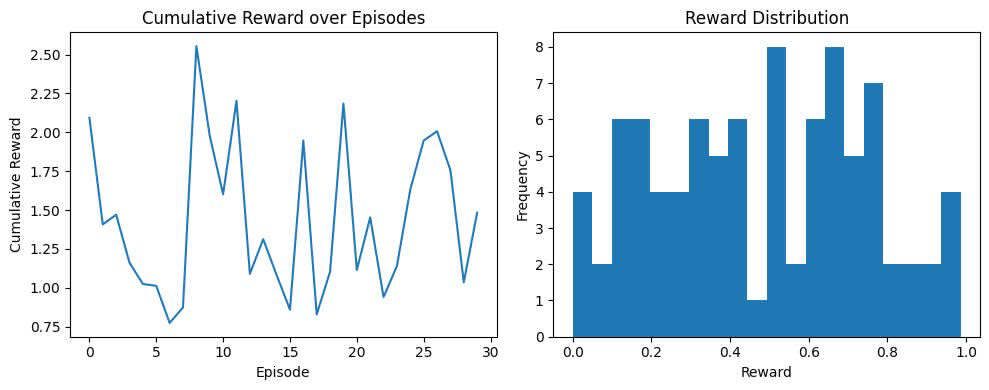
\includegraphics[width=436.75pt,height=172.25pt]{latexImage_4fb7453db8fd5e13f0f2b8e0448fad75.png}}
\put(72.8,-408.811){\fontsize{11}{1}\usefont{T1}{cmr}{m}{n}\selectfont\color{color_80434}训}
\put(83.8,-408.811){\fontsize{11}{1}\usefont{T1}{cmr}{m}{n}\selectfont\color{color_80434}练}
\put(97,-408.811){\fontsize{11}{1}\usefont{T1}{ptm}{m}{n}\selectfont\color{color_80434}40}
\put(110.2,-408.811){\fontsize{11}{1}\usefont{T1}{cmr}{m}{n}\selectfont\color{color_80434}轮}
\put(121.2,-408.811){\fontsize{11}{1}\usefont{T1}{cmr}{m}{n}\selectfont\color{color_80434}结果如下}
\put(165.2,-408.811){\fontsize{11}{1}\usefont{T1}{ptm}{m}{n}\selectfont\color{color_80434}:}
\put(72.65,-602.411){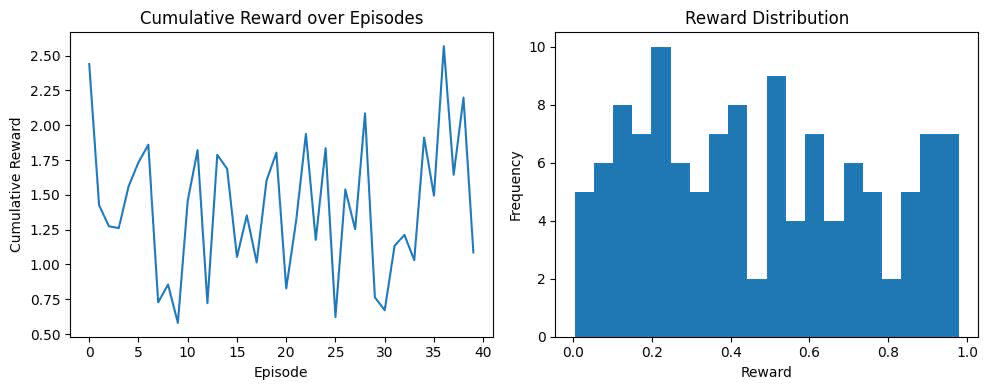
\includegraphics[width=436.75pt,height=172.4pt]{latexImage_00c0c45b3034211a38f4ea0b6ebb8c8a.png}}
\put(56,-615.711){\fontsize{11}{1}\usefont{T1}{ptm}{m}{n}\selectfont\color{color_80434} }
\put(58.695,-615.711){\fontsize{11}{1}\usefont{T1}{ptm}{m}{n}\selectfont\color{color_80434} }
\put(61.489,-615.711){\fontsize{11}{1}\usefont{T1}{ptm}{m}{n}\selectfont\color{color_80434} }
\put(64.184,-615.711){\fontsize{11}{1}\usefont{T1}{ptm}{m}{n}\selectfont\color{color_80434} }
\put(66.978,-615.711){\fontsize{11}{1}\usefont{T1}{ptm}{m}{n}\selectfont\color{color_80434} }
\put(69.673,-615.711){\fontsize{11}{1}\usefont{T1}{ptm}{m}{n}\selectfont\color{color_80434} }
\put(72.5,-615.711){\fontsize{11}{1}\usefont{T1}{cmr}{m}{n}\selectfont\color{color_80434}训}
\put(83.5,-615.711){\fontsize{11}{1}\usefont{T1}{cmr}{m}{n}\selectfont\color{color_80434}练}
\put(96.7,-615.711){\fontsize{11}{1}\usefont{T1}{ptm}{m}{n}\selectfont\color{color_80434}50}
\put(109.9,-615.711){\fontsize{11}{1}\usefont{T1}{cmr}{m}{n}\selectfont\color{color_80434}轮}
\put(120.9,-615.711){\fontsize{11}{1}\usefont{T1}{cmr}{m}{n}\selectfont\color{color_80434}结果如下}
\put(164.9,-615.711){\fontsize{11}{1}\usefont{T1}{ptm}{m}{n}\selectfont\color{color_80434}:}
\end{picture}
\begin{tikzpicture}[overlay]
\path(0pt,0pt);
\draw[color_29791,line width=1.5pt,line join=round]
(509.45pt, -123.811pt) -- (72.7pt, -123.811pt)
;
\end{tikzpicture}
\newpage
\begin{tikzpicture}[overlay]
\path(0pt,0pt);
\draw[color_29791,line width=1.5pt,line join=round]
(509.45pt, -123.811pt) -- (72.7pt, -123.811pt)
;
\begin{scope}
\clip
(55.799pt, -240.711pt) -- (509.498pt, -240.711pt)
 -- (509.498pt, -240.711pt)
 -- (509.498pt, -61.51099pt)
 -- (509.498pt, -61.51099pt)
 -- (55.799pt, -61.51099pt) -- cycle
;
\end{scope}
\end{tikzpicture}
\begin{picture}(-5,0)(2.5,0)
\put(55.85,-240.561){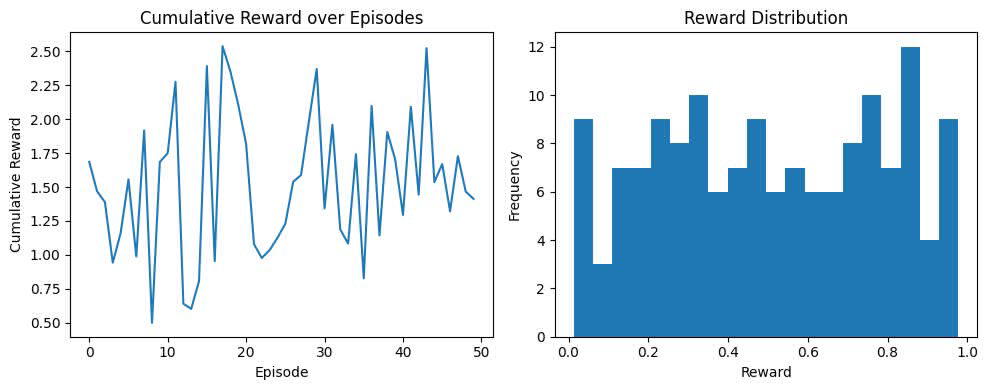
\includegraphics[width=453.55pt,height=179.05pt]{latexImage_28c06a74fff1491e73f2336337223aa3.png}}
\put(56,-253.911){\fontsize{11}{1}\usefont{T1}{ptm}{m}{n}\selectfont\color{color_80434} }
\put(58.695,-253.911){\fontsize{11}{1}\usefont{T1}{ptm}{m}{n}\selectfont\color{color_80434} }
\put(61.489,-253.911){\fontsize{11}{1}\usefont{T1}{ptm}{m}{n}\selectfont\color{color_80434} }
\put(64.184,-253.911){\fontsize{11}{1}\usefont{T1}{ptm}{m}{n}\selectfont\color{color_80434} }
\put(66.978,-253.911){\fontsize{11}{1}\usefont{T1}{ptm}{m}{n}\selectfont\color{color_80434} }
\put(69.673,-253.911){\fontsize{11}{1}\usefont{T1}{ptm}{m}{n}\selectfont\color{color_80434} }
\put(72.5,-253.911){\fontsize{11}{1}\usefont{T1}{cmr}{m}{n}\selectfont\color{color_80434}训}
\put(83.5,-253.911){\fontsize{11}{1}\usefont{T1}{cmr}{m}{n}\selectfont\color{color_80434}练}
\put(96.7,-253.911){\fontsize{11}{1}\usefont{T1}{ptm}{m}{n}\selectfont\color{color_80434}60}
\put(109.9,-253.911){\fontsize{11}{1}\usefont{T1}{cmr}{m}{n}\selectfont\color{color_80434}轮}
\put(120.9,-253.911){\fontsize{11}{1}\usefont{T1}{cmr}{m}{n}\selectfont\color{color_80434}结果如下}
\put(164.9,-253.911){\fontsize{11}{1}\usefont{T1}{ptm}{m}{n}\selectfont\color{color_80434}:}
\put(55.85,-453.911){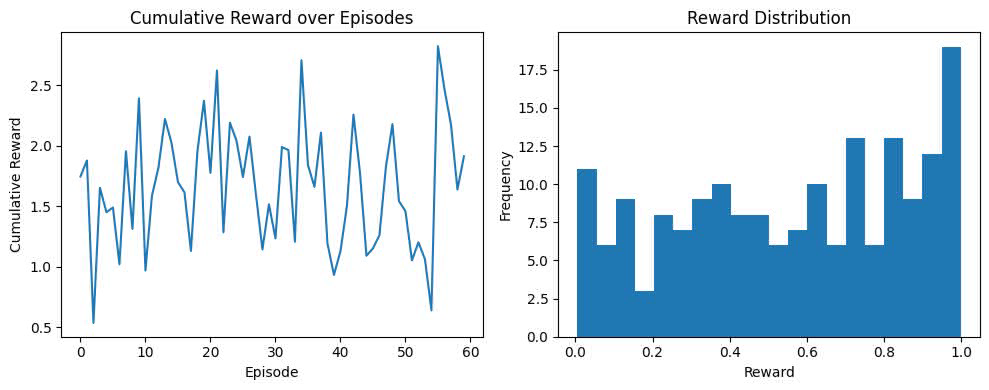
\includegraphics[width=453.55pt,height=178.85pt]{latexImage_5c20e4b25da19d55d11bb17b38f7a7df.png}}
\put(56,-467.211){\fontsize{11}{1}\usefont{T1}{cmr}{m}{n}\selectfont\color{color_80434}训}
\put(67,-467.211){\fontsize{11}{1}\usefont{T1}{cmr}{m}{n}\selectfont\color{color_80434}练}
\put(80.2,-467.211){\fontsize{11}{1}\usefont{T1}{ptm}{m}{n}\selectfont\color{color_80434}70}
\put(93.4,-467.211){\fontsize{11}{1}\usefont{T1}{cmr}{m}{n}\selectfont\color{color_80434}轮}
\put(104.4,-467.211){\fontsize{11}{1}\usefont{T1}{cmr}{m}{n}\selectfont\color{color_80434}结果如下}
\put(148.4,-467.211){\fontsize{11}{1}\usefont{T1}{ptm}{m}{n}\selectfont\color{color_80434}:}
\put(55.85,-667.261){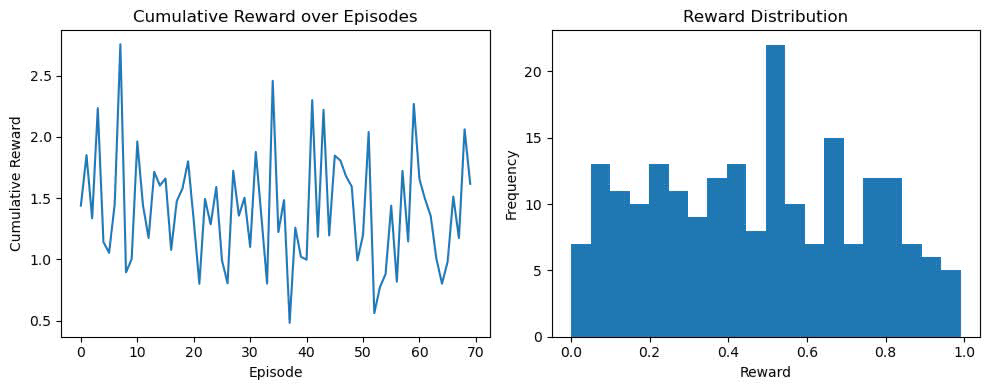
\includegraphics[width=453.55pt,height=178.85pt]{latexImage_7126c71d1a41a896bc1158350a77380a.png}}
\end{picture}
\newpage
\begin{tikzpicture}[overlay]\path(0pt,0pt);\end{tikzpicture}
\begin{picture}(-5,0)(2.5,0)
\put(78,-92.211){\fontsize{16}{1}\usefont{T1}{ptm}{b}{n}\selectfont\color{color_55609}4}
\put(86,-92.211){\fontsize{16}{1}\usefont{T1}{cmr}{m}{n}\selectfont\color{color_55609}、}
\put(119,-92.211){\fontsize{16}{1}\usefont{T1}{cmr}{m}{n}\selectfont\color{color_55609}模型的分析与改进}
\put(56,-122.311){\fontsize{11}{1}\usefont{T1}{cmr}{m}{n}\selectfont\color{color_80434}}
\put(72.8,-122.311){\fontsize{11}{1}\usefont{T1}{cmr}{m}{n}\selectfont\color{color_80434}分析}
\put(94.8,-122.311){\fontsize{11}{1}\usefont{T1}{ptm}{m}{n}\selectfont\color{color_80434}:}
\put(78,-139.111){\fontsize{12}{1}\usefont{T1}{cmr}{m}{n}\selectfont\color{color_29791}¡}
\put(94.8,-139.111){\fontsize{11}{1}\usefont{T1}{cmr}{m}{n}\selectfont\color{color_80434}根据累}
\put(127.8,-139.111){\fontsize{11}{1}\usefont{T1}{cmr}{m}{n}\selectfont\color{color_80434}积}
\put(138.8,-139.111){\fontsize{11}{1}\usefont{T1}{cmr}{m}{n}\selectfont\color{color_80434}奖励曲}
\put(171.8,-139.111){\fontsize{11}{1}\usefont{T1}{cmr}{m}{n}\selectfont\color{color_80434}线}
\put(182.8,-139.111){\fontsize{11}{1}\usefont{T1}{cmr}{m}{n}\selectfont\color{color_80434}和}
\put(193.8,-139.111){\fontsize{12}{1}\usefont{T1}{cmr}{m}{n}\selectfont\color{color_29791}奖励}
\put(217.8,-139.111){\fontsize{12}{1}\usefont{T1}{cmr}{m}{n}\selectfont\color{color_29791}分布}
\put(241.8,-139.111){\fontsize{12}{1}\usefont{T1}{cmr}{m}{n}\selectfont\color{color_29791}直}
\put(253.8,-139.111){\fontsize{12}{1}\usefont{T1}{cmr}{m}{n}\selectfont\color{color_29791}方}
\put(265.8,-139.111){\fontsize{12}{1}\usefont{T1}{cmr}{m}{n}\selectfont\color{color_29791}图}
\put(277.8,-139.111){\fontsize{12}{1}\usefont{T1}{cmr}{m}{n}\selectfont\color{color_29791},}
\put(281.6,-139.111){\fontsize{12}{1}\usefont{T1}{cmr}{m}{n}\selectfont\color{color_29791}我}
\put(293.6,-139.111){\fontsize{12}{1}\usefont{T1}{cmr}{m}{n}\selectfont\color{color_29791}们可以}
\put(329.6,-139.111){\fontsize{12}{1}\usefont{T1}{cmr}{m}{n}\selectfont\color{color_29791}知道}
\put(353.6,-139.111){\fontsize{12}{1}\usefont{T1}{cmr}{m}{n}\selectfont\color{color_29791},}
\put(357.4,-139.111){\fontsize{12}{1}\usefont{T1}{cmr}{m}{n}\selectfont\color{color_29791}随着}
\put(381.4,-139.111){\fontsize{12}{1}\usefont{T1}{cmr}{m}{n}\selectfont\color{color_29791}训}
\put(393.4,-139.111){\fontsize{12}{1}\usefont{T1}{cmr}{m}{n}\selectfont\color{color_29791}练}
\put(405.4,-139.111){\fontsize{12}{1}\usefont{T1}{cmr}{m}{n}\selectfont\color{color_29791}次}
\put(417.4,-139.111){\fontsize{12}{1}\usefont{T1}{cmr}{m}{n}\selectfont\color{color_29791}数的}
\put(441.4,-139.111){\fontsize{12}{1}\usefont{T1}{cmr}{m}{n}\selectfont\color{color_29791}增}
\put(453.4,-139.111){\fontsize{12}{1}\usefont{T1}{cmr}{m}{n}\selectfont\color{color_29791}加}
\put(465.4,-139.111){\fontsize{12}{1}\usefont{T1}{cmr}{m}{n}\selectfont\color{color_29791},}
\put(469.2,-139.111){\fontsize{12}{1}\usefont{T1}{cmr}{m}{n}\selectfont\color{color_29791}对}
\put(481.2,-139.111){\fontsize{12}{1}\usefont{T1}{cmr}{m}{n}\selectfont\color{color_29791}每}
\put(493.2,-139.111){\fontsize{12}{1}\usefont{T1}{cmr}{m}{n}\selectfont\color{color_29791}个}
\put(94.8,-153.111){\fontsize{12}{1}\usefont{T1}{cmr}{m}{n}\selectfont\color{color_29791}潜水器的}
\put(142.8,-153.111){\fontsize{12}{1}\usefont{T1}{cmr}{m}{n}\selectfont\color{color_29791}运}
\put(154.8,-153.111){\fontsize{12}{1}\usefont{T1}{cmr}{m}{n}\selectfont\color{color_29791}动}
\put(166.8,-153.111){\fontsize{12}{1}\usefont{T1}{cmr}{m}{n}\selectfont\color{color_29791}姿}
\put(178.8,-153.111){\fontsize{12}{1}\usefont{T1}{cmr}{m}{n}\selectfont\color{color_29791}态的预测性}
\put(238.8,-153.111){\fontsize{12}{1}\usefont{T1}{cmr}{m}{n}\selectfont\color{color_29791}就}
\put(250.8,-153.111){\fontsize{12}{1}\usefont{T1}{cmr}{m}{n}\selectfont\color{color_29791}会}
\put(262.8,-153.111){\fontsize{12}{1}\usefont{T1}{cmr}{m}{n}\selectfont\color{color_29791}更加准确}
\put(310.8,-153.111){\fontsize{12}{1}\usefont{T1}{cmr}{m}{n}\selectfont\color{color_29791},}
\put(314.6,-153.111){\fontsize{12}{1}\usefont{T1}{cmr}{m}{n}\selectfont\color{color_29791}观测上}
\put(350.6,-153.111){\fontsize{12}{1}\usefont{T1}{cmr}{m}{n}\selectfont\color{color_29791}图会}
\put(374.6,-153.111){\fontsize{12}{1}\usefont{T1}{cmr}{m}{n}\selectfont\color{color_29791}发现}
\put(398.6,-153.111){\fontsize{12}{1}\usefont{T1}{cmr}{m}{n}\selectfont\color{color_29791}整体训}
\put(434.6,-153.111){\fontsize{12}{1}\usefont{T1}{cmr}{m}{n}\selectfont\color{color_29791}练}
\put(446.6,-153.111){\fontsize{12}{1}\usefont{T1}{cmr}{m}{n}\selectfont\color{color_29791}效果比较}
\put(494.6,-153.111){\fontsize{12}{1}\usefont{T1}{cmr}{m}{n}\selectfont\color{color_29791}平}
\put(94.8,-167.111){\fontsize{12}{1}\usefont{T1}{cmr}{m}{n}\selectfont\color{color_29791}稳}
\put(106.8,-167.111){\fontsize{12}{1}\usefont{T1}{cmr}{m}{n}\selectfont\color{color_29791},}
\put(110.6,-167.111){\fontsize{12}{1}\usefont{T1}{cmr}{m}{n}\selectfont\color{color_29791}即使面对不同的环境}
\put(218.6,-167.111){\fontsize{12}{1}\usefont{T1}{cmr}{m}{n}\selectfont\color{color_29791}也}
\put(230.6,-167.111){\fontsize{12}{1}\usefont{T1}{cmr}{m}{n}\selectfont\color{color_29791}能}
\put(242.6,-167.111){\fontsize{12}{1}\usefont{T1}{cmr}{m}{n}\selectfont\color{color_29791}保}
\put(254.6,-167.111){\fontsize{12}{1}\usefont{T1}{cmr}{m}{n}\selectfont\color{color_29791}持良}
\put(278.6,-167.111){\fontsize{12}{1}\usefont{T1}{cmr}{m}{n}\selectfont\color{color_29791}好}
\put(290.6,-167.111){\fontsize{12}{1}\usefont{T1}{cmr}{m}{n}\selectfont\color{color_29791}的一}
\put(314.6,-167.111){\fontsize{12}{1}\usefont{T1}{cmr}{m}{n}\selectfont\color{color_29791}致}
\put(326.6,-167.111){\fontsize{12}{1}\usefont{T1}{cmr}{m}{n}\selectfont\color{color_29791}性}
\put(338.6,-167.111){\fontsize{12}{1}\usefont{T1}{cmr}{m}{n}\selectfont\color{color_29791}.}
\put(78,-183.211){\fontsize{11}{1}\usefont{T1}{cmr}{m}{n}\selectfont\color{color_80434}¡}
\put(94.8,-183.211){\fontsize{11}{1}\usefont{T1}{cmr}{m}{n}\selectfont\color{color_80434}建议}
\put(116.8,-183.211){\fontsize{11}{1}\usefont{T1}{cmr}{m}{n}\selectfont\color{color_80434}选取}
\put(138.8,-183.211){\fontsize{11}{1}\usefont{T1}{cmr}{m}{n}\selectfont\color{color_80434}更多的数据集进行}
\put(226.8,-183.211){\fontsize{11}{1}\usefont{T1}{cmr}{m}{n}\selectfont\color{color_80434}训}
\put(237.8,-183.211){\fontsize{11}{1}\usefont{T1}{cmr}{m}{n}\selectfont\color{color_80434}练}
\put(248.8,-183.211){\fontsize{11}{1}\usefont{T1}{ptm}{m}{n}\selectfont\color{color_80434},}
\put(251.5,-183.211){\fontsize{11}{1}\usefont{T1}{cmr}{m}{n}\selectfont\color{color_80434}增}
\put(262.5,-183.211){\fontsize{11}{1}\usefont{T1}{cmr}{m}{n}\selectfont\color{color_80434}加}
\put(273.5,-183.211){\fontsize{11}{1}\usefont{T1}{cmr}{m}{n}\selectfont\color{color_80434}迭代}
\put(295.5,-183.211){\fontsize{11}{1}\usefont{T1}{cmr}{m}{n}\selectfont\color{color_80434}次}
\put(306.5,-183.211){\fontsize{11}{1}\usefont{T1}{cmr}{m}{n}\selectfont\color{color_80434}数}
\put(317.5,-183.211){\fontsize{11}{1}\usefont{T1}{cmr}{m}{n}\selectfont\color{color_80434}来}
\put(328.5,-183.211){\fontsize{11}{1}\usefont{T1}{cmr}{m}{n}\selectfont\color{color_80434}达}
\put(339.5,-183.211){\fontsize{11}{1}\usefont{T1}{cmr}{m}{n}\selectfont\color{color_80434}到更}
\put(361.5,-183.211){\fontsize{11}{1}\usefont{T1}{cmr}{m}{n}\selectfont\color{color_80434}好}
\put(372.5,-183.211){\fontsize{11}{1}\usefont{T1}{cmr}{m}{n}\selectfont\color{color_80434}的效果}
\put(405.5,-183.211){\fontsize{11}{1}\usefont{T1}{ptm}{m}{n}\selectfont\color{color_80434}.}
\put(56,-199.011){\fontsize{11}{1}\usefont{T1}{cmr}{m}{n}\selectfont\color{color_80434}}
\put(72.8,-199.011){\fontsize{11}{1}\usefont{T1}{cmr}{m}{n}\selectfont\color{color_80434}改进}
\put(94.8,-199.011){\fontsize{11}{1}\usefont{T1}{ptm}{m}{n}\selectfont\color{color_80434}:}
\end{picture}
\newpage
\begin{tikzpicture}[overlay]\path(0pt,0pt);\end{tikzpicture}
\begin{picture}(-5,0)(2.5,0)
\put(78,-76.01099){\fontsize{11}{1}\usefont{T1}{cmr}{m}{n}\selectfont\color{color_80434}¡}
\put(94.8,-76.01099){\fontsize{12}{1}\usefont{T1}{cmr}{m}{n}\selectfont\color{color_84742}1}
\put(104.8,-76.01099){\fontsize{12}{1}\usefont{T1}{cmr}{m}{n}\selectfont\color{color_84742}在环境模型、}
\put(176.8,-76.01099){\fontsize{12}{1}\usefont{T1}{cmr}{m}{n}\selectfont\color{color_84742}智}
\put(188.8,-76.01099){\fontsize{12}{1}\usefont{T1}{cmr}{m}{n}\selectfont\color{color_84742}能}
\put(200.8,-76.01099){\fontsize{12}{1}\usefont{T1}{cmr}{m}{n}\selectfont\color{color_84742}体}
\put(212.8,-76.01099){\fontsize{12}{1}\usefont{T1}{cmr}{m}{n}\selectfont\color{color_84742}设计和学}
\put(260.8,-76.01099){\fontsize{12}{1}\usefont{T1}{cmr}{m}{n}\selectfont\color{color_84742}习}
\put(272.8,-76.01099){\fontsize{12}{1}\usefont{T1}{cmr}{m}{n}\selectfont\color{color_84742}算法确定后,使用}
\put(368.8,-76.01099){\fontsize{12}{1}\usefont{T1}{cmr}{m}{n}\selectfont\color{color_84742}历史}
\put(392.8,-76.01099){\fontsize{12}{1}\usefont{T1}{cmr}{m}{n}\selectfont\color{color_84742}数据对}
\put(428.8,-76.01099){\fontsize{12}{1}\usefont{T1}{cmr}{m}{n}\selectfont\color{color_84742}智}
\put(440.8,-76.01099){\fontsize{12}{1}\usefont{T1}{cmr}{m}{n}\selectfont\color{color_84742}能}
\put(452.8,-76.01099){\fontsize{12}{1}\usefont{T1}{cmr}{m}{n}\selectfont\color{color_84742}体}
\put(464.8,-76.01099){\fontsize{12}{1}\usefont{T1}{cmr}{m}{n}\selectfont\color{color_84742}进行}
\put(488.8,-76.01099){\fontsize{12}{1}\usefont{T1}{cmr}{m}{n}\selectfont\color{color_84742}训}
\put(94.8,-96.51099){\fontsize{12}{1}\usefont{T1}{cmr}{m}{n}\selectfont\color{color_84742}练}
\put(106.8,-96.51099){\fontsize{12}{1}\usefont{T1}{cmr}{m}{n}\selectfont\color{color_84742},}
\put(110.6,-96.51099){\fontsize{12}{1}\usefont{T1}{cmr}{m}{n}\selectfont\color{color_84742}并不}
\put(134.6,-96.51099){\fontsize{12}{1}\usefont{T1}{cmr}{m}{n}\selectfont\color{color_84742}断}
\put(146.6,-96.51099){\fontsize{12}{1}\usefont{T1}{cmr}{m}{n}\selectfont\color{color_84742}优化}
\put(170.6,-96.51099){\fontsize{12}{1}\usefont{T1}{cmr}{m}{n}\selectfont\color{color_84742}智}
\put(182.6,-96.51099){\fontsize{12}{1}\usefont{T1}{cmr}{m}{n}\selectfont\color{color_84742}能}
\put(194.6,-96.51099){\fontsize{12}{1}\usefont{T1}{cmr}{m}{n}\selectfont\color{color_84742}体}
\put(206.6,-96.51099){\fontsize{12}{1}\usefont{T1}{cmr}{m}{n}\selectfont\color{color_84742}的}
\put(218.6,-96.51099){\fontsize{12}{1}\usefont{T1}{cmr}{m}{n}\selectfont\color{color_84742}策略}
\put(242.6,-96.51099){\fontsize{12}{1}\usefont{T1}{cmr}{m}{n}\selectfont\color{color_84742},}
\put(246.4,-96.51099){\fontsize{12}{1}\usefont{T1}{cmr}{m}{n}\selectfont\color{color_84742}以最}
\put(270.4,-96.51099){\fontsize{12}{1}\usefont{T1}{cmr}{m}{n}\selectfont\color{color_84742}大}
\put(282.4,-96.51099){\fontsize{12}{1}\usefont{T1}{cmr}{m}{n}\selectfont\color{color_84742}化累}
\put(306.4,-96.51099){\fontsize{12}{1}\usefont{T1}{cmr}{m}{n}\selectfont\color{color_84742}积}
\put(318.4,-96.51099){\fontsize{12}{1}\usefont{T1}{cmr}{m}{n}\selectfont\color{color_84742}奖励}
\put(342.4,-96.51099){\fontsize{12}{1}\usefont{T1}{cmr}{m}{n}\selectfont\color{color_84742}.}
\put(78,-117.011){\fontsize{11}{1}\usefont{T1}{cmr}{m}{n}\selectfont\color{color_80434}¡}
\put(94.8,-117.011){\fontsize{12}{1}\usefont{T1}{cmr}{m}{n}\selectfont\color{color_84742} }
\put(98.6,-117.011){\fontsize{12}{1}\usefont{T1}{cmr}{m}{n}\selectfont\color{color_84742}通过在仿真环境中进行测}
\put(230.6,-117.011){\fontsize{12}{1}\usefont{T1}{cmr}{m}{n}\selectfont\color{color_84742}试}
\put(242.6,-117.011){\fontsize{12}{1}\usefont{T1}{cmr}{m}{n}\selectfont\color{color_84742}和验证}
\put(278.6,-117.011){\fontsize{12}{1}\usefont{T1}{cmr}{m}{n}\selectfont\color{color_84742},}
\put(282.4,-117.011){\fontsize{12}{1}\usefont{T1}{cmr}{m}{n}\selectfont\color{color_84742}评估训}
\put(318.4,-117.011){\fontsize{12}{1}\usefont{T1}{cmr}{m}{n}\selectfont\color{color_84742}练}
\put(330.4,-117.011){\fontsize{12}{1}\usefont{T1}{cmr}{m}{n}\selectfont\color{color_84742}好}
\put(342.4,-117.011){\fontsize{12}{1}\usefont{T1}{cmr}{m}{n}\selectfont\color{color_84742}的}
\put(354.4,-117.011){\fontsize{12}{1}\usefont{T1}{cmr}{m}{n}\selectfont\color{color_84742}智}
\put(366.4,-117.011){\fontsize{12}{1}\usefont{T1}{cmr}{m}{n}\selectfont\color{color_84742}能}
\put(378.4,-117.011){\fontsize{12}{1}\usefont{T1}{cmr}{m}{n}\selectfont\color{color_84742}体}
\put(390.4,-117.011){\fontsize{12}{1}\usefont{T1}{cmr}{m}{n}\selectfont\color{color_84742}在}
\put(402.4,-117.011){\fontsize{12}{1}\usefont{T1}{cmr}{m}{n}\selectfont\color{color_84742}实际}
\put(426.4,-117.011){\fontsize{12}{1}\usefont{T1}{cmr}{m}{n}\selectfont\color{color_84742}场}
\put(438.4,-117.011){\fontsize{12}{1}\usefont{T1}{cmr}{m}{n}\selectfont\color{color_84742}景中的性能}
\put(498.4,-117.011){\fontsize{12}{1}\usefont{T1}{cmr}{m}{n}\selectfont\color{color_84742},}
\put(94.8,-137.511){\fontsize{12}{1}\usefont{T1}{cmr}{m}{n}\selectfont\color{color_84742}并根据需要进行}
\put(178.8,-137.511){\fontsize{12}{1}\usefont{T1}{cmr}{m}{n}\selectfont\color{color_84742}调整}
\put(202.8,-137.511){\fontsize{12}{1}\usefont{T1}{cmr}{m}{n}\selectfont\color{color_84742}和优化}
\put(238.8,-137.511){\fontsize{12}{1}\usefont{T1}{cmr}{m}{n}\selectfont\color{color_84742}.}
\put(56,-180.411){\fontsize{18}{1}\usefont{T1}{cmr}{m}{n}\selectfont\color{color_55609}八}
\put(74,-180.411){\fontsize{18}{1}\usefont{T1}{cmr}{m}{n}\selectfont\color{color_55609}、}
\put(98,-180.411){\fontsize{18}{1}\usefont{T1}{cmr}{m}{n}\selectfont\color{color_55609}敏感性分析}
\put(56,-229.111){\fontsize{12}{1}\usefont{T1}{cmr}{m}{n}\selectfont\color{color_84742}分析}
\put(80,-229.111){\fontsize{12}{1}\usefont{T1}{cmr}{m}{n}\selectfont\color{color_84742}:}
\put(56,-246.111){\fontsize{12}{1}\usefont{T1}{cmr}{m}{n}\selectfont\color{color_84742}}
\put(72.8,-246.111){\fontsize{12}{1}\usefont{T1}{cmr}{m}{n}\selectfont\color{color_84742}基于}
\put(99.2,-246.111){\fontsize{12}{1}\usefont{T1}{cmr}{m}{n}\selectfont\color{color_84742}K}
\put(106.796,-246.111){\fontsize{12}{1}\usefont{T1}{cmr}{m}{n}\selectfont\color{color_84742}a}
\put(114.188,-246.111){\fontsize{12}{1}\usefont{T1}{cmr}{m}{n}\selectfont\color{color_84742}l}
\put(117.488,-246.111){\fontsize{12}{1}\usefont{T1}{cmr}{m}{n}\selectfont\color{color_84742}ma}
\put(136.568,-246.111){\fontsize{12}{1}\usefont{T1}{cmr}{m}{n}\selectfont\color{color_84742}n}
\put(146.6,-246.111){\fontsize{12}{1}\usefont{T1}{cmr}{m}{n}\selectfont\color{color_84742}滤波算法改进后的动态预测模型模拟潜水器位置在}
\put(410.6,-246.111){\fontsize{12}{1}\usefont{T1}{cmr}{m}{n}\selectfont\color{color_84742}实际}
\put(434.6,-246.111){\fontsize{12}{1}\usefont{T1}{cmr}{m}{n}\selectfont\color{color_84742}应用中需要}
\put(494.6,-246.111){\fontsize{12}{1}\usefont{T1}{cmr}{m}{n}\selectfont\color{color_84742}实}
\put(72.8,-260.111){\fontsize{12}{1}\usefont{T1}{cmr}{m}{n}\selectfont\color{color_84742}时更新}
\put(108.8,-260.111){\fontsize{12}{1}\usefont{T1}{cmr}{m}{n}\selectfont\color{color_84742},}
\put(112.6,-260.111){\fontsize{12}{1}\usefont{T1}{cmr}{m}{n}\selectfont\color{color_84742}总体来}
\put(148.6,-260.111){\fontsize{12}{1}\usefont{T1}{cmr}{m}{n}\selectfont\color{color_84742}说}
\put(160.6,-260.111){\fontsize{12}{1}\usefont{T1}{cmr}{m}{n}\selectfont\color{color_84742},}
\put(164.4,-260.111){\fontsize{12}{1}\usefont{T1}{cmr}{m}{n}\selectfont\color{color_84742}模型预测与}
\put(224.4,-260.111){\fontsize{12}{1}\usefont{T1}{cmr}{m}{n}\selectfont\color{color_84742}事}
\put(236.4,-260.111){\fontsize{12}{1}\usefont{T1}{cmr}{m}{n}\selectfont\color{color_84742}先给定}
\put(272.4,-260.111){\fontsize{12}{1}\usefont{T1}{cmr}{m}{n}\selectfont\color{color_84742}路}
\put(284.4,-260.111){\fontsize{12}{1}\usefont{T1}{cmr}{m}{n}\selectfont\color{color_84742}径}
\put(296.4,-260.111){\fontsize{12}{1}\usefont{T1}{cmr}{m}{n}\selectfont\color{color_84742}基本}
\put(320.4,-260.111){\fontsize{12}{1}\usefont{T1}{cmr}{m}{n}\selectfont\color{color_84742}吻}
\put(332.4,-260.111){\fontsize{12}{1}\usefont{T1}{cmr}{m}{n}\selectfont\color{color_84742}合}
\put(344.4,-260.111){\fontsize{12}{1}\usefont{T1}{cmr}{m}{n}\selectfont\color{color_84742},}
\put(348.2,-260.111){\fontsize{12}{1}\usefont{T1}{cmr}{m}{n}\selectfont\color{color_84742}波动性较}
\put(396.2,-260.111){\fontsize{12}{1}\usefont{T1}{cmr}{m}{n}\selectfont\color{color_84742}小}
\put(56,-294.111){\fontsize{11}{1}\usefont{T1}{cmr}{m}{n}\selectfont\color{color_80434}}
\put(96.8,-294.111){\fontsize{12}{1}\usefont{T1}{cmr}{m}{n}\selectfont\color{color_84742} }
\put(72.8,-294.111){\fontsize{12}{1}\usefont{T1}{cmr}{m}{n}\selectfont\color{color_84742}使用}
\put(100.6,-294.111){\fontsize{12}{1}\usefont{T1}{cmr}{m}{n}\selectfont\color{color_84742}D}
\put(109.804,-294.111){\fontsize{12}{1}\usefont{T1}{cmr}{m}{n}\selectfont\color{color_84742}e}
\put(117.196,-294.111){\fontsize{12}{1}\usefont{T1}{cmr}{m}{n}\selectfont\color{color_84742}e}
\put(124.588,-294.111){\fontsize{12}{1}\usefont{T1}{cmr}{m}{n}\selectfont\color{color_84742}p}
\put(132.184,-294.111){\fontsize{12}{1}\usefont{T1}{cmr}{m}{n}\selectfont\color{color_84742}-}
\put(136.972,-294.111){\fontsize{12}{1}\usefont{T1}{cmr}{m}{n}\selectfont\color{color_84742}Q}
\put(146.764,-294.111){\fontsize{12}{1}\usefont{T1}{cmr}{m}{n}\selectfont\color{color_84742}-}
\put(151.06,-294.111){\fontsize{12}{1}\usefont{T1}{cmr}{m}{n}\selectfont\color{color_84742}L}
\put(157.456,-294.111){\fontsize{12}{1}\usefont{T1}{cmr}{m}{n}\selectfont\color{color_84742}e}
\put(164.848,-294.111){\fontsize{12}{1}\usefont{T1}{cmr}{m}{n}\selectfont\color{color_84742}a}
\put(172.24,-294.111){\fontsize{12}{1}\usefont{T1}{cmr}{m}{n}\selectfont\color{color_84742}r}
\put(176.944,-294.111){\fontsize{12}{1}\usefont{T1}{cmr}{m}{n}\selectfont\color{color_84742}ni}
\put(187.84,-294.111){\fontsize{12}{1}\usefont{T1}{cmr}{m}{n}\selectfont\color{color_84742}ng}
\put(205.6,-294.111){\fontsize{12}{1}\usefont{T1}{cmr}{m}{n}\selectfont\color{color_84742}算法}
\put(229.6,-294.111){\fontsize{12}{1}\usefont{T1}{cmr}{m}{n}\selectfont\color{color_84742}来处}
\put(253.6,-294.111){\fontsize{12}{1}\usefont{T1}{cmr}{m}{n}\selectfont\color{color_84742}理多个潜水器的}
\put(337.6,-294.111){\fontsize{12}{1}\usefont{T1}{cmr}{m}{n}\selectfont\color{color_84742}移}
\put(349.6,-294.111){\fontsize{12}{1}\usefont{T1}{cmr}{m}{n}\selectfont\color{color_84742}动问题,}
\put(397.6,-294.111){\fontsize{12}{1}\usefont{T1}{cmr}{m}{n}\selectfont\color{color_84742}考虑}
\put(421.6,-294.111){\fontsize{12}{1}\usefont{T1}{cmr}{m}{n}\selectfont\color{color_84742}到了潜水器之间}
\put(72.8,-308.111){\fontsize{12}{1}\usefont{T1}{cmr}{m}{n}\selectfont\color{color_84742}的}
\put(84.8,-308.111){\fontsize{12}{1}\usefont{T1}{cmr}{m}{n}\selectfont\color{color_84742}协}
\put(96.8,-308.111){\fontsize{12}{1}\usefont{T1}{cmr}{m}{n}\selectfont\color{color_84742}作}
\put(108.8,-308.111){\fontsize{12}{1}\usefont{T1}{cmr}{m}{n}\selectfont\color{color_84742}和}
\put(120.8,-308.111){\fontsize{12}{1}\usefont{T1}{cmr}{m}{n}\selectfont\color{color_84742}竞争}
\put(144.8,-308.111){\fontsize{12}{1}\usefont{T1}{cmr}{m}{n}\selectfont\color{color_84742}关系,}
\put(180.8,-308.111){\fontsize{12}{1}\usefont{T1}{cmr}{m}{n}\selectfont\color{color_84742}从}
\put(192.8,-308.111){\fontsize{12}{1}\usefont{T1}{cmr}{m}{n}\selectfont\color{color_84742}而更}
\put(216.8,-308.111){\fontsize{12}{1}\usefont{T1}{cmr}{m}{n}\selectfont\color{color_84742}好}
\put(228.8,-308.111){\fontsize{12}{1}\usefont{T1}{cmr}{m}{n}\selectfont\color{color_84742}地优化}
\put(264.8,-308.111){\fontsize{12}{1}\usefont{T1}{cmr}{m}{n}\selectfont\color{color_84742}整体}
\put(288.8,-308.111){\fontsize{12}{1}\usefont{T1}{cmr}{m}{n}\selectfont\color{color_84742}的搜寻效率和定位准确}
\put(408.8,-308.111){\fontsize{12}{1}\usefont{T1}{cmr}{m}{n}\selectfont\color{color_84742}度}
\put(420.8,-308.111){\fontsize{12}{1}\usefont{T1}{cmr}{m}{n}\selectfont\color{color_84742},}
\put(424.6,-308.111){\fontsize{12}{1}\usefont{T1}{cmr}{m}{n}\selectfont\color{color_84742}如果}
\put(448.6,-308.111){\fontsize{12}{1}\usefont{T1}{cmr}{m}{n}\selectfont\color{color_84742}继续}
\put(472.6,-308.111){\fontsize{12}{1}\usefont{T1}{cmr}{m}{n}\selectfont\color{color_84742}优化参}
\put(72.8,-322.111){\fontsize{12}{1}\usefont{T1}{cmr}{m}{n}\selectfont\color{color_84742}数}
\put(84.8,-322.111){\fontsize{12}{1}\usefont{T1}{cmr}{m}{n}\selectfont\color{color_84742},}
\put(88.6,-322.111){\fontsize{12}{1}\usefont{T1}{cmr}{m}{n}\selectfont\color{color_84742}迭代}
\put(112.6,-322.111){\fontsize{12}{1}\usefont{T1}{cmr}{m}{n}\selectfont\color{color_84742}一定}
\put(136.6,-322.111){\fontsize{12}{1}\usefont{T1}{cmr}{m}{n}\selectfont\color{color_84742}次}
\put(148.6,-322.111){\fontsize{12}{1}\usefont{T1}{cmr}{m}{n}\selectfont\color{color_84742}数之后}
\put(184.6,-322.111){\fontsize{12}{1}\usefont{T1}{cmr}{m}{n}\selectfont\color{color_84742},}
\put(188.4,-322.111){\fontsize{12}{1}\usefont{T1}{cmr}{m}{n}\selectfont\color{color_84742}模型的准确性}
\put(260.4,-322.111){\fontsize{12}{1}\usefont{T1}{cmr}{m}{n}\selectfont\color{color_84742}会}
\put(272.4,-322.111){\fontsize{12}{1}\usefont{T1}{cmr}{m}{n}\selectfont\color{color_84742}更高}
\put(56,-344.711){\fontsize{18}{1}\usefont{T1}{cmr}{m}{n}\selectfont\color{color_55609}九}
\put(74,-344.711){\fontsize{18}{1}\usefont{T1}{cmr}{m}{n}\selectfont\color{color_55609}、}
\put(98,-344.711){\fontsize{18}{1}\usefont{T1}{cmr}{m}{n}\selectfont\color{color_55609}模型}
\put(134,-344.711){\fontsize{18}{1}\usefont{T1}{cmr}{m}{n}\selectfont\color{color_55609}评}
\put(152,-344.711){\fontsize{18}{1}\usefont{T1}{cmr}{m}{n}\selectfont\color{color_55609}价}
\put(170,-344.711){\fontsize{18}{1}\usefont{T1}{cmr}{m}{n}\selectfont\color{color_55609}与推}
\put(206,-344.711){\fontsize{18}{1}\usefont{T1}{cmr}{m}{n}\selectfont\color{color_55609}广}
\put(78,-378.511){\fontsize{16}{1}\usefont{T1}{ptm}{b}{n}\selectfont\color{color_55609}1}
\put(86,-378.511){\fontsize{16}{1}\usefont{T1}{cmr}{m}{n}\selectfont\color{color_55609}、}
\put(119,-378.511){\fontsize{16}{1}\usefont{T1}{cmr}{m}{n}\selectfont\color{color_55609}优}
\put(135,-378.511){\fontsize{16}{1}\usefont{T1}{cmr}{m}{n}\selectfont\color{color_55609}势}
\put(56,-408.611){\fontsize{11}{1}\usefont{T1}{cmr}{m}{n}\selectfont\color{color_80434}}
\put(72.8,-408.611){\fontsize{11}{1}\usefont{T1}{cmr}{m}{n}\selectfont\color{color_80434}轻}
\put(83.8,-408.611){\fontsize{11}{1}\usefont{T1}{cmr}{m}{n}\selectfont\color{color_80434}量}
\put(94.8,-408.611){\fontsize{11}{1}\usefont{T1}{cmr}{m}{n}\selectfont\color{color_80434}级}
\put(105.8,-408.611){\fontsize{11}{1}\usefont{T1}{cmr}{m}{n}\selectfont\color{color_80434}:}
\put(116.8,-408.611){\fontsize{11}{1}\usefont{T1}{cmr}{m}{n}\selectfont\color{color_80434}模型结}
\put(149.8,-408.611){\fontsize{11}{1}\usefont{T1}{cmr}{m}{n}\selectfont\color{color_80434}构}
\put(160.8,-408.611){\fontsize{11}{1}\usefont{T1}{cmr}{m}{n}\selectfont\color{color_80434}相对简}
\put(193.8,-408.611){\fontsize{11}{1}\usefont{T1}{cmr}{m}{n}\selectfont\color{color_80434}单}
\put(204.8,-408.611){\fontsize{11}{1}\usefont{T1}{cmr}{m}{n}\selectfont\color{color_80434},}
\put(215.8,-408.611){\fontsize{11}{1}\usefont{T1}{cmr}{m}{n}\selectfont\color{color_80434}兼}
\put(226.8,-408.611){\fontsize{11}{1}\usefont{T1}{cmr}{m}{n}\selectfont\color{color_80434}容}
\put(237.8,-408.611){\fontsize{11}{1}\usefont{T1}{cmr}{m}{n}\selectfont\color{color_80434}较多}
\put(259.8,-408.611){\fontsize{11}{1}\usefont{T1}{cmr}{m}{n}\selectfont\color{color_80434}实际}
\put(281.8,-408.611){\fontsize{11}{1}\usefont{T1}{cmr}{m}{n}\selectfont\color{color_80434}因素,}
\put(314.8,-408.611){\fontsize{11}{1}\usefont{T1}{cmr}{m}{n}\selectfont\color{color_80434}适}
\put(325.8,-408.611){\fontsize{11}{1}\usefont{T1}{cmr}{m}{n}\selectfont\color{color_80434}当引}
\put(347.8,-408.611){\fontsize{11}{1}\usefont{T1}{cmr}{m}{n}\selectfont\color{color_80434}入工}
\put(369.8,-408.611){\fontsize{11}{1}\usefont{T1}{cmr}{m}{n}\selectfont\color{color_80434}程设计方面理论,优化}
\put(479.8,-408.611){\fontsize{11}{1}\usefont{T1}{cmr}{m}{n}\selectfont\color{color_80434}度}
\put(490.8,-408.611){\fontsize{11}{1}\usefont{T1}{cmr}{m}{n}\selectfont\color{color_80434}高}
\put(56,-424.411){\fontsize{11}{1}\usefont{T1}{cmr}{m}{n}\selectfont\color{color_80434}}
\put(72.8,-424.411){\fontsize{11}{1}\usefont{T1}{cmr}{m}{n}\selectfont\color{color_80434}创造}
\put(94.8,-424.411){\fontsize{11}{1}\usefont{T1}{cmr}{m}{n}\selectfont\color{color_80434}性:}
\put(116.8,-424.411){\fontsize{11}{1}\usefont{T1}{cmr}{m}{n}\selectfont\color{color_80434}创}
\put(127.8,-424.411){\fontsize{11}{1}\usefont{T1}{cmr}{m}{n}\selectfont\color{color_80434}建了一些}
\put(171.8,-424.411){\fontsize{11}{1}\usefont{T1}{cmr}{m}{n}\selectfont\color{color_80434}衡}
\put(182.8,-424.411){\fontsize{11}{1}\usefont{T1}{cmr}{m}{n}\selectfont\color{color_80434}量}
\put(193.8,-424.411){\fontsize{11}{1}\usefont{T1}{cmr}{m}{n}\selectfont\color{color_80434}指标,分析结果可以定}
\put(303.8,-424.411){\fontsize{11}{1}\usefont{T1}{cmr}{m}{n}\selectfont\color{color_80434}量}
\put(314.8,-424.411){\fontsize{11}{1}\usefont{T1}{cmr}{m}{n}\selectfont\color{color_80434}验证,这}
\put(358.8,-424.411){\fontsize{11}{1}\usefont{T1}{cmr}{m}{n}\selectfont\color{color_80434}也}
\put(369.8,-424.411){\fontsize{11}{1}\usefont{T1}{cmr}{m}{n}\selectfont\color{color_80434}使}
\put(380.8,-424.411){\fontsize{11}{1}\usefont{T1}{cmr}{m}{n}\selectfont\color{color_80434}我}
\put(391.8,-424.411){\fontsize{11}{1}\usefont{T1}{cmr}{m}{n}\selectfont\color{color_80434}们的模型}
\put(435.8,-424.411){\fontsize{11}{1}\usefont{T1}{cmr}{m}{n}\selectfont\color{color_80434}具}
\put(446.8,-424.411){\fontsize{11}{1}\usefont{T1}{cmr}{m}{n}\selectfont\color{color_80434}有}
\put(457.8,-424.411){\fontsize{11}{1}\usefont{T1}{cmr}{m}{n}\selectfont\color{color_80434}科}
\put(468.8,-424.411){\fontsize{11}{1}\usefont{T1}{cmr}{m}{n}\selectfont\color{color_80434}学性}
\put(56,-440.211){\fontsize{11}{1}\usefont{T1}{cmr}{m}{n}\selectfont\color{color_80434}}
\put(72.8,-440.211){\fontsize{11}{1}\usefont{T1}{cmr}{m}{n}\selectfont\color{color_80434}准确性:}
\put(116.8,-440.211){\fontsize{11}{1}\usefont{T1}{cmr}{m}{n}\selectfont\color{color_80434}模型结论}
\put(160.8,-440.211){\fontsize{11}{1}\usefont{T1}{cmr}{m}{n}\selectfont\color{color_80434}均}
\put(171.8,-440.211){\fontsize{11}{1}\usefont{T1}{cmr}{m}{n}\selectfont\color{color_80434}与相应仿真数据相}
\put(259.8,-440.211){\fontsize{11}{1}\usefont{T1}{cmr}{m}{n}\selectfont\color{color_80434}吻}
\put(270.8,-440.211){\fontsize{11}{1}\usefont{T1}{cmr}{m}{n}\selectfont\color{color_80434}合,}
\put(292.8,-440.211){\fontsize{11}{1}\usefont{T1}{cmr}{m}{n}\selectfont\color{color_80434}互}
\put(303.8,-440.211){\fontsize{11}{1}\usefont{T1}{cmr}{m}{n}\selectfont\color{color_80434}相}
\put(314.8,-440.211){\fontsize{11}{1}\usefont{T1}{cmr}{m}{n}\selectfont\color{color_80434}印}
\put(325.8,-440.211){\fontsize{11}{1}\usefont{T1}{cmr}{m}{n}\selectfont\color{color_80434}证,且}
\put(358.8,-440.211){\fontsize{11}{1}\usefont{T1}{cmr}{m}{n}\selectfont\color{color_80434}逻辑自洽}
\put(402.8,-440.211){\fontsize{11}{1}\usefont{T1}{cmr}{m}{n}\selectfont\color{color_80434}实}
\put(413.8,-440.211){\fontsize{11}{1}\usefont{T1}{cmr}{m}{n}\selectfont\color{color_80434}用}
\put(56,-456.011){\fontsize{11}{1}\usefont{T1}{cmr}{m}{n}\selectfont\color{color_80434}}
\put(72.8,-456.011){\fontsize{11}{1}\usefont{T1}{cmr}{m}{n}\selectfont\color{color_80434}稳}
\put(83.8,-456.011){\fontsize{11}{1}\usefont{T1}{cmr}{m}{n}\selectfont\color{color_80434}定性:}
\put(116.8,-456.011){\fontsize{11}{1}\usefont{T1}{cmr}{m}{n}\selectfont\color{color_80434}模型基}
\put(149.8,-456.011){\fontsize{11}{1}\usefont{T1}{cmr}{m}{n}\selectfont\color{color_80434}础}
\put(160.8,-456.011){\fontsize{11}{1}\usefont{T1}{cmr}{m}{n}\selectfont\color{color_80434}经}
\put(171.8,-456.011){\fontsize{11}{1}\usefont{T1}{cmr}{m}{n}\selectfont\color{color_80434}过敏感性分析测}
\put(248.8,-456.011){\fontsize{11}{1}\usefont{T1}{cmr}{m}{n}\selectfont\color{color_80434}试}
\put(259.8,-456.011){\fontsize{11}{1}\usefont{T1}{cmr}{m}{n}\selectfont\color{color_80434},}
\put(270.8,-456.011){\fontsize{11}{1}\usefont{T1}{cmr}{m}{n}\selectfont\color{color_80434}误差是}
\put(303.8,-456.011){\fontsize{11}{1}\usefont{T1}{cmr}{m}{n}\selectfont\color{color_80434}可以}
\put(325.8,-456.011){\fontsize{11}{1}\usefont{T1}{cmr}{m}{n}\selectfont\color{color_80434}接}
\put(336.8,-456.011){\fontsize{11}{1}\usefont{T1}{cmr}{m}{n}\selectfont\color{color_80434}受的,}
\put(369.8,-456.011){\fontsize{11}{1}\usefont{T1}{cmr}{m}{n}\selectfont\color{color_80434}所}
\put(380.8,-456.011){\fontsize{11}{1}\usefont{T1}{cmr}{m}{n}\selectfont\color{color_80434}以模型}
\put(413.8,-456.011){\fontsize{11}{1}\usefont{T1}{cmr}{m}{n}\selectfont\color{color_80434}是}
\put(424.8,-456.011){\fontsize{11}{1}\usefont{T1}{cmr}{m}{n}\selectfont\color{color_80434}稳}
\put(435.8,-456.011){\fontsize{11}{1}\usefont{T1}{cmr}{m}{n}\selectfont\color{color_80434}定的}
\put(78,-476.611){\fontsize{16}{1}\usefont{T1}{ptm}{b}{n}\selectfont\color{color_55609}2}
\put(86,-476.611){\fontsize{16}{1}\usefont{T1}{cmr}{m}{n}\selectfont\color{color_55609}、}
\put(119,-476.611){\fontsize{16}{1}\usefont{T1}{cmr}{m}{n}\selectfont\color{color_55609}模型的}
\put(167,-476.611){\fontsize{16}{1}\usefont{T1}{cmr}{m}{n}\selectfont\color{color_55609}局}
\put(183,-476.611){\fontsize{16}{1}\usefont{T1}{cmr}{m}{n}\selectfont\color{color_55609}限}
\put(199,-476.611){\fontsize{16}{1}\usefont{T1}{cmr}{m}{n}\selectfont\color{color_55609}性与}
\put(231,-476.611){\fontsize{16}{1}\usefont{T1}{cmr}{m}{n}\selectfont\color{color_55609}拓}
\put(247,-476.611){\fontsize{16}{1}\usefont{T1}{cmr}{m}{n}\selectfont\color{color_55609}展}
\put(56,-506.711){\fontsize{11}{1}\usefont{T1}{cmr}{m}{n}\selectfont\color{color_80434}我}
\put(67,-506.711){\fontsize{11}{1}\usefont{T1}{cmr}{m}{n}\selectfont\color{color_80434}们的模型有以下}
\put(144,-506.711){\fontsize{11}{1}\usefont{T1}{cmr}{m}{n}\selectfont\color{color_80434}局}
\put(155,-506.711){\fontsize{11}{1}\usefont{T1}{cmr}{m}{n}\selectfont\color{color_80434}限}
\put(166,-506.711){\fontsize{11}{1}\usefont{T1}{cmr}{m}{n}\selectfont\color{color_80434}性和相关改进}
\put(232,-506.711){\fontsize{11}{1}\usefont{T1}{ptm}{m}{n}\selectfont\color{color_80434}:}
\put(56,-526.411){\fontsize{11}{1}\usefont{T1}{cmr}{m}{n}\selectfont\color{color_80434}}
\put(72.8,-526.411){\fontsize{11}{1}\usefont{T1}{cmr}{m}{n}\selectfont\color{color_80434}忽略}
\put(94.8,-526.411){\fontsize{11}{1}\usefont{T1}{cmr}{m}{n}\selectfont\color{color_80434}了一些}
\put(127.8,-526.411){\fontsize{11}{1}\usefont{T1}{cmr}{m}{n}\selectfont\color{color_80434}极端天}
\put(160.8,-526.411){\fontsize{11}{1}\usefont{T1}{cmr}{m}{n}\selectfont\color{color_80434}气,洋流}
\put(204.8,-526.411){\fontsize{11}{1}\usefont{T1}{ptm}{m}{n}\selectfont\color{color_80434},}
\put(207.5,-526.411){\fontsize{11}{1}\usefont{T1}{cmr}{m}{n}\selectfont\color{color_80434}地}
\put(218.5,-526.411){\fontsize{11}{1}\usefont{T1}{cmr}{m}{n}\selectfont\color{color_80434}形}
\put(229.5,-526.411){\fontsize{11}{1}\usefont{T1}{cmr}{m}{n}\selectfont\color{color_80434}等不确定因素的}
\put(306.5,-526.411){\fontsize{11}{1}\usefont{T1}{cmr}{m}{n}\selectfont\color{color_80434}干扰}
\put(328.5,-526.411){\fontsize{11}{1}\usefont{T1}{ptm}{m}{n}\selectfont\color{color_80434},}
\put(331.3,-526.411){\fontsize{11}{1}\usefont{T1}{cmr}{m}{n}\selectfont\color{color_80434}降低}
\put(353.3,-526.411){\fontsize{11}{1}\usefont{T1}{cmr}{m}{n}\selectfont\color{color_80434}了模型的置信}
\put(419.3,-526.411){\fontsize{11}{1}\usefont{T1}{cmr}{m}{n}\selectfont\color{color_80434}度}
\put(56,-549.911){\fontsize{11}{1}\usefont{T1}{cmr}{m}{n}\selectfont\color{color_80434}}
\put(72.8,-549.911){\fontsize{11}{1}\usefont{T1}{cmr}{m}{n}\selectfont\color{color_80434}模型参数为模拟参数}
\put(171.8,-549.911){\fontsize{11}{1}\usefont{T1}{ptm}{m}{n}\selectfont\color{color_80434},}
\put(174.5,-549.911){\fontsize{11}{1}\usefont{T1}{cmr}{m}{n}\selectfont\color{color_80434}并}
\put(185.5,-549.911){\fontsize{11}{1}\usefont{T1}{cmr}{m}{n}\selectfont\color{color_80434}未}
\put(196.5,-549.911){\fontsize{11}{1}\usefont{T1}{cmr}{m}{n}\selectfont\color{color_80434}根据真}
\put(229.5,-549.911){\fontsize{11}{1}\usefont{T1}{cmr}{m}{n}\selectfont\color{color_80434}实}
\put(240.5,-549.911){\fontsize{11}{1}\usefont{T1}{cmr}{m}{n}\selectfont\color{color_80434}数据集进行}
\put(295.5,-549.911){\fontsize{11}{1}\usefont{T1}{cmr}{m}{n}\selectfont\color{color_80434}训}
\put(306.5,-549.911){\fontsize{11}{1}\usefont{T1}{cmr}{m}{n}\selectfont\color{color_80434}练}
\put(317.5,-549.911){\fontsize{11}{1}\usefont{T1}{ptm}{m}{n}\selectfont\color{color_80434},}
\put(320.3,-549.911){\fontsize{11}{1}\usefont{T1}{cmr}{m}{n}\selectfont\color{color_80434}准确}
\put(342.3,-549.911){\fontsize{11}{1}\usefont{T1}{cmr}{m}{n}\selectfont\color{color_80434}度}
\put(353.3,-549.911){\fontsize{11}{1}\usefont{T1}{cmr}{m}{n}\selectfont\color{color_80434}可以}
\put(375.3,-549.911){\fontsize{11}{1}\usefont{T1}{cmr}{m}{n}\selectfont\color{color_80434}继续}
\put(397.3,-549.911){\fontsize{11}{1}\usefont{T1}{cmr}{m}{n}\selectfont\color{color_80434}提}
\put(408.3,-549.911){\fontsize{11}{1}\usefont{T1}{cmr}{m}{n}\selectfont\color{color_80434}升}
\put(56,-573.411){\fontsize{11}{1}\usefont{T1}{cmr}{m}{n}\selectfont\color{color_80434}}
\put(72.8,-573.411){\fontsize{11}{1}\usefont{T1}{cmr}{m}{n}\selectfont\color{color_80434}我}
\put(83.8,-573.411){\fontsize{11}{1}\usefont{T1}{cmr}{m}{n}\selectfont\color{color_80434}们}
\put(94.8,-573.411){\fontsize{11}{1}\usefont{T1}{cmr}{m}{n}\selectfont\color{color_80434}只}
\put(105.8,-573.411){\fontsize{11}{1}\usefont{T1}{cmr}{m}{n}\selectfont\color{color_80434}是}
\put(116.8,-573.411){\fontsize{11}{1}\usefont{T1}{cmr}{m}{n}\selectfont\color{color_80434}对}
\put(127.8,-573.411){\fontsize{11}{1}\usefont{T1}{cmr}{m}{n}\selectfont\color{color_80434}初始}
\put(149.8,-573.411){\fontsize{11}{1}\usefont{T1}{cmr}{m}{n}\selectfont\color{color_80434}化模型进行一定的优化}
\put(259.8,-573.411){\fontsize{11}{1}\usefont{T1}{ptm}{m}{n}\selectfont\color{color_80434},}
\put(262.5,-573.411){\fontsize{11}{1}\usefont{T1}{cmr}{m}{n}\selectfont\color{color_80434}模型}
\put(284.5,-573.411){\fontsize{11}{1}\usefont{T1}{cmr}{m}{n}\selectfont\color{color_80434}迭代}
\put(306.5,-573.411){\fontsize{11}{1}\usefont{T1}{cmr}{m}{n}\selectfont\color{color_80434}次}
\put(317.5,-573.411){\fontsize{11}{1}\usefont{T1}{cmr}{m}{n}\selectfont\color{color_80434}数较少}
\put(350.5,-573.411){\fontsize{11}{1}\usefont{T1}{ptm}{m}{n}\selectfont\color{color_80434},}
\put(353.3,-573.411){\fontsize{11}{1}\usefont{T1}{cmr}{m}{n}\selectfont\color{color_80434}实}
\put(364.3,-573.411){\fontsize{11}{1}\usefont{T1}{cmr}{m}{n}\selectfont\color{color_80434}践}
\put(375.3,-573.411){\fontsize{11}{1}\usefont{T1}{cmr}{m}{n}\selectfont\color{color_80434}性有}
\put(397.3,-573.411){\fontsize{11}{1}\usefont{T1}{cmr}{m}{n}\selectfont\color{color_80434}待}
\put(408.3,-573.411){\fontsize{11}{1}\usefont{T1}{cmr}{m}{n}\selectfont\color{color_80434}考}
\put(419.3,-573.411){\fontsize{11}{1}\usefont{T1}{cmr}{m}{n}\selectfont\color{color_80434}察}
\put(430.3,-573.411){\fontsize{11}{1}\usefont{T1}{cmr}{m}{n}\selectfont\color{color_80434}和改进}
\put(56,-596.911){\fontsize{11}{1}\usefont{T1}{cmr}{m}{n}\selectfont\color{color_80434}}
\put(72.8,-596.911){\fontsize{11}{1}\usefont{T1}{cmr}{m}{n}\selectfont\color{color_80434}可能部分模型}
\put(138.8,-596.911){\fontsize{11}{1}\usefont{T1}{cmr}{m}{n}\selectfont\color{color_80434}选取}
\put(160.8,-596.911){\fontsize{11}{1}\usefont{T1}{cmr}{m}{n}\selectfont\color{color_80434}比较}
\put(182.8,-596.911){\fontsize{11}{1}\usefont{T1}{cmr}{m}{n}\selectfont\color{color_80434}局}
\put(193.8,-596.911){\fontsize{11}{1}\usefont{T1}{cmr}{m}{n}\selectfont\color{color_80434}限}
\put(204.8,-596.911){\fontsize{11}{1}\usefont{T1}{ptm}{m}{n}\selectfont\color{color_80434},}
\put(207.5,-596.911){\fontsize{11}{1}\usefont{T1}{cmr}{m}{n}\selectfont\color{color_80434}比如成本效益比率在在使用}
\put(339.5,-596.911){\fontsize{11}{1}\usefont{T1}{cmr}{m}{n}\selectfont\color{color_80434}蒙}
\put(350.5,-596.911){\fontsize{11}{1}\usefont{T1}{cmr}{m}{n}\selectfont\color{color_80434}特}
\put(361.5,-596.911){\fontsize{11}{1}\usefont{T1}{cmr}{m}{n}\selectfont\color{color_80434}卡洛}
\put(383.5,-596.911){\fontsize{11}{1}\usefont{T1}{cmr}{m}{n}\selectfont\color{color_80434}算法模拟时}
\put(438.5,-596.911){\fontsize{11}{1}\usefont{T1}{ptm}{m}{n}\selectfont\color{color_80434},}
\put(441.3,-596.911){\fontsize{11}{1}\usefont{T1}{cmr}{m}{n}\selectfont\color{color_80434}因为}
\put(463.3,-596.911){\fontsize{11}{1}\usefont{T1}{cmr}{m}{n}\selectfont\color{color_80434}没}
\put(474.3,-596.911){\fontsize{11}{1}\usefont{T1}{cmr}{m}{n}\selectfont\color{color_80434}有给定}
\put(72.8,-617.411){\fontsize{11}{1}\usefont{T1}{cmr}{m}{n}\selectfont\color{color_80434}准确的要}
\put(116.8,-617.411){\fontsize{11}{1}\usefont{T1}{cmr}{m}{n}\selectfont\color{color_80434}求}
\put(127.8,-617.411){\fontsize{11}{1}\usefont{T1}{ptm}{m}{n}\selectfont\color{color_80434},}
\put(130.5,-617.411){\fontsize{11}{1}\usefont{T1}{cmr}{m}{n}\selectfont\color{color_80434}导致}
\put(152.5,-617.411){\fontsize{11}{1}\usefont{T1}{cmr}{m}{n}\selectfont\color{color_80434}后}
\put(163.5,-617.411){\fontsize{11}{1}\usefont{T1}{cmr}{m}{n}\selectfont\color{color_80434}续}
\put(174.5,-617.411){\fontsize{11}{1}\usefont{T1}{cmr}{m}{n}\selectfont\color{color_80434}模型的应用性较}
\put(251.5,-617.411){\fontsize{11}{1}\usefont{T1}{cmr}{m}{n}\selectfont\color{color_80434}低}
\put(262.5,-617.411){\fontsize{11}{1}\usefont{T1}{ptm}{m}{n}\selectfont\color{color_80434},}
\put(265.3,-617.411){\fontsize{11}{1}\usefont{T1}{cmr}{m}{n}\selectfont\color{color_80434}有}
\put(276.3,-617.411){\fontsize{11}{1}\usefont{T1}{cmr}{m}{n}\selectfont\color{color_80434}待}
\put(287.3,-617.411){\fontsize{11}{1}\usefont{T1}{cmr}{m}{n}\selectfont\color{color_80434}改进}
\end{picture}
\begin{tikzpicture}[overlay]
\path(0pt,0pt);
\draw[color_29791,line width=1.5pt,line join=round]
(509.45pt, -144.311pt) -- (77.9pt, -144.311pt)
;
\draw[color_29791,line width=1.5pt,line join=round]
(509.45pt, -144.311pt) -- (77.9pt, -144.311pt)
;
\end{tikzpicture}
\newpage
\begin{tikzpicture}[overlay]\path(0pt,0pt);\end{tikzpicture}
\begin{picture}(-5,0)(2.5,0)
\put(219.8,-78.31097){\fontsize{18}{1}\usefont{T1}{cmr}{m}{n}\selectfont\color{color_55609}备}
\put(237.8,-78.31097){\fontsize{18}{1}\usefont{T1}{cmr}{m}{n}\selectfont\color{color_55609}忘录}
\put(273.8,-78.31097){\fontsize{18}{1}\usefont{T1}{cmr}{m}{n}\selectfont\color{color_55609}(}
\put(291.8,-78.31097){\fontsize{18}{1}\usefont{T1}{cmr}{m}{n}\selectfont\color{color_55609}两}
\put(309.8,-78.31097){\fontsize{18}{1}\usefont{T1}{cmr}{m}{n}\selectfont\color{color_55609}页}
\put(327.8,-78.31097){\fontsize{18}{1}\usefont{T1}{cmr}{m}{n}\selectfont\color{color_55609})}
\end{picture}
\newpage
\begin{tikzpicture}[overlay]\path(0pt,0pt);\end{tikzpicture}
\begin{picture}(-5,0)(2.5,0)
\put(56,-78.31097){\fontsize{18}{1}\usefont{T1}{cmr}{m}{n}\selectfont\color{color_55609}参}
\put(74,-78.31097){\fontsize{18}{1}\usefont{T1}{cmr}{m}{n}\selectfont\color{color_55609}考}
\put(92,-78.31097){\fontsize{18}{1}\usefont{T1}{cmr}{m}{n}\selectfont\color{color_55609}文}
\put(110,-78.31097){\fontsize{18}{1}\usefont{T1}{cmr}{m}{n}\selectfont\color{color_55609}献}
\put(56,-110.411){\fontsize{11}{1}\usefont{T1}{ptm}{m}{n}\selectfont\color{color_80434}[}
\put(59.597,-110.411){\fontsize{11}{1}\usefont{T1}{ptm}{m}{n}\selectfont\color{color_80434}1]}
\put(200.8,-110.411){\fontsize{11}{1}\usefont{T1}{cmr}{m}{n}\selectfont\color{color_80434} }
\put(68.8,-110.411){\fontsize{11}{1}\usefont{T1}{cmr}{m}{n}\selectfont\color{color_80434}朱}
\put(79.8,-110.411){\fontsize{11}{1}\usefont{T1}{cmr}{m}{n}\selectfont\color{color_80434}敏,}
\put(101.8,-110.411){\fontsize{11}{1}\usefont{T1}{cmr}{m}{n}\selectfont\color{color_80434}张}
\put(112.8,-110.411){\fontsize{11}{1}\usefont{T1}{cmr}{m}{n}\selectfont\color{color_80434}同}
\put(123.8,-110.411){\fontsize{11}{1}\usefont{T1}{cmr}{m}{n}\selectfont\color{color_80434}伟}
\put(134.8,-110.411){\fontsize{11}{1}\usefont{T1}{cmr}{m}{n}\selectfont\color{color_80434},}
\put(145.8,-110.411){\fontsize{11}{1}\usefont{T1}{cmr}{m}{n}\selectfont\color{color_80434}杨}
\put(156.8,-110.411){\fontsize{11}{1}\usefont{T1}{cmr}{m}{n}\selectfont\color{color_80434}波,等}
\put(189.8,-110.411){\fontsize{11}{1}\usefont{T1}{cmr}{m}{n}\selectfont\color{color_80434}.}
\put(204.287,-110.411){\fontsize{11}{1}\usefont{T1}{cmr}{m}{n}\selectfont\color{color_80434}蛟龙}
\put(226.3,-110.411){\fontsize{11}{1}\usefont{T1}{cmr}{m}{n}\selectfont\color{color_80434}号载人}
\put(259.3,-110.411){\fontsize{11}{1}\usefont{T1}{cmr}{m}{n}\selectfont\color{color_80434}潜水器声学系}
\put(325.3,-110.411){\fontsize{11}{1}\usefont{T1}{cmr}{m}{n}\selectfont\color{color_80434}统}
\put(336.3,-110.411){\fontsize{11}{1}\usefont{T1}{cmr}{m}{n}\selectfont\color{color_80434}[}
\put(347.3,-110.411){\fontsize{11}{1}\usefont{T1}{ptm}{m}{n}\selectfont\color{color_80434}J}
\put(373.6,-110.411){\fontsize{11}{1}\usefont{T1}{cmr}{m}{n}\selectfont\color{color_80434} }
\put(351.6,-110.411){\fontsize{11}{1}\usefont{T1}{cmr}{m}{n}\selectfont\color{color_80434}].}
\put(377.087,-110.411){\fontsize{11}{1}\usefont{T1}{cmr}{m}{n}\selectfont\color{color_80434}科}
\put(388.1,-110.411){\fontsize{11}{1}\usefont{T1}{cmr}{m}{n}\selectfont\color{color_80434}学通}
\put(410.1,-110.411){\fontsize{11}{1}\usefont{T1}{cmr}{m}{n}\selectfont\color{color_80434}报}
\put(421.1,-110.411){\fontsize{11}{1}\usefont{T1}{cmr}{m}{n}\selectfont\color{color_80434},}
\put(432.1,-110.411){\fontsize{11}{1}\usefont{T1}{ptm}{m}{n}\selectfont\color{color_80434}2014}
\put(454.1,-110.411){\fontsize{11}{1}\usefont{T1}{cmr}{m}{n}\selectfont\color{color_80434},}
\put(465.1,-110.411){\fontsize{11}{1}\usefont{T1}{ptm}{m}{n}\selectfont\color{color_80434}59(}
\put(479.785,-110.411){\fontsize{11}{1}\usefont{T1}{ptm}{m}{n}\selectfont\color{color_80434} }
\put(482.48,-110.411){\fontsize{11}{1}\usefont{T1}{ptm}{m}{n}\selectfont\color{color_80434}35)}
\put(497.165,-110.411){\fontsize{11}{1}\usefont{T1}{ptm}{m}{n}\selectfont\color{color_80434} }
\put(499.959,-110.411){\fontsize{11}{1}\usefont{T1}{ptm}{m}{n}\selectfont\color{color_80434}:}
\put(502.962,-110.411){\fontsize{11}{1}\usefont{T1}{ptm}{m}{n}\selectfont\color{color_80434} }
\put(56,-123.311){\fontsize{11}{1}\usefont{T1}{ptm}{m}{n}\selectfont\color{color_80434}3462}
\put(78,-123.311){\fontsize{11}{1}\usefont{T1}{cmr}{m}{n}\selectfont\color{color_80434}-}
\put(89,-123.311){\fontsize{11}{1}\usefont{T1}{ptm}{m}{n}\selectfont\color{color_80434}3470}
\put(111,-123.311){\fontsize{11}{1}\usefont{T1}{cmr}{m}{n}\selectfont\color{color_80434}.}
\put(56,-142.911){\fontsize{11}{1}\usefont{T1}{ptm}{m}{n}\selectfont\color{color_80434}[}
\put(59.597,-142.911){\fontsize{11}{1}\usefont{T1}{ptm}{m}{n}\selectfont\color{color_80434}2]}
\put(222.8,-142.911){\fontsize{11}{1}\usefont{T1}{cmr}{m}{n}\selectfont\color{color_80434} }
\put(68.8,-142.911){\fontsize{11}{1}\usefont{T1}{cmr}{m}{n}\selectfont\color{color_80434}张}
\put(79.8,-142.911){\fontsize{11}{1}\usefont{T1}{cmr}{m}{n}\selectfont\color{color_80434}同}
\put(90.8,-142.911){\fontsize{11}{1}\usefont{T1}{cmr}{m}{n}\selectfont\color{color_80434}伟}
\put(101.8,-142.911){\fontsize{11}{1}\usefont{T1}{cmr}{m}{n}\selectfont\color{color_80434},}
\put(112.8,-142.911){\fontsize{11}{1}\usefont{T1}{cmr}{m}{n}\selectfont\color{color_80434}刘烨瑶}
\put(145.8,-142.911){\fontsize{11}{1}\usefont{T1}{cmr}{m}{n}\selectfont\color{color_80434},}
\put(156.8,-142.911){\fontsize{11}{1}\usefont{T1}{cmr}{m}{n}\selectfont\color{color_80434}唐嘉陵}
\put(189.8,-142.911){\fontsize{11}{1}\usefont{T1}{cmr}{m}{n}\selectfont\color{color_80434},等}
\put(211.8,-142.911){\fontsize{11}{1}\usefont{T1}{cmr}{m}{n}\selectfont\color{color_80434}.}
\put(226.3,-142.911){\fontsize{11}{1}\usefont{T1}{cmr}{m}{n}\selectfont\color{color_80434}大深度载人}
\put(281.3,-142.911){\fontsize{11}{1}\usefont{T1}{cmr}{m}{n}\selectfont\color{color_80434}潜水器之}
\put(325.3,-142.911){\fontsize{11}{1}\usefont{T1}{cmr}{m}{n}\selectfont\color{color_80434}超短}
\put(347.3,-142.911){\fontsize{11}{1}\usefont{T1}{cmr}{m}{n}\selectfont\color{color_80434}基}
\put(358.3,-142.911){\fontsize{11}{1}\usefont{T1}{cmr}{m}{n}\selectfont\color{color_80434}线}
\put(369.3,-142.911){\fontsize{11}{1}\usefont{T1}{cmr}{m}{n}\selectfont\color{color_80434}定位系}
\put(402.3,-142.911){\fontsize{11}{1}\usefont{T1}{cmr}{m}{n}\selectfont\color{color_80434}统}
\put(413.3,-142.911){\fontsize{11}{1}\usefont{T1}{ptm}{m}{n}\selectfont\color{color_80434}:}
\put(416.391,-142.911){\fontsize{11}{1}\usefont{T1}{ptm}{m}{n}\selectfont\color{color_80434} }
\put(419.1,-142.911){\fontsize{11}{1}\usefont{T1}{cmr}{m}{n}\selectfont\color{color_80434}海上}
\put(441.1,-142.911){\fontsize{11}{1}\usefont{T1}{cmr}{m}{n}\selectfont\color{color_80434}试}
\put(452.1,-142.911){\fontsize{11}{1}\usefont{T1}{cmr}{m}{n}\selectfont\color{color_80434}验及}
\put(474.1,-142.911){\fontsize{11}{1}\usefont{T1}{cmr}{m}{n}\selectfont\color{color_80434}载人深}
\put(56,-163.411){\fontsize{11}{1}\usefont{T1}{cmr}{m}{n}\selectfont\color{color_80434}潜应用}
\put(89,-163.411){\fontsize{11}{1}\usefont{T1}{cmr}{m}{n}\selectfont\color{color_80434}[}
\put(100,-163.411){\fontsize{11}{1}\usefont{T1}{ptm}{m}{n}\selectfont\color{color_80434}J}
\put(104.202,-163.411){\fontsize{11}{1}\usefont{T1}{ptm}{m}{n}\selectfont\color{color_80434}/}
\put(107.293,-163.411){\fontsize{11}{1}\usefont{T1}{ptm}{m}{n}\selectfont\color{color_80434}O}
\put(115.191,-163.411){\fontsize{11}{1}\usefont{T1}{ptm}{m}{n}\selectfont\color{color_80434}L}
\put(144,-163.411){\fontsize{11}{1}\usefont{T1}{cmr}{m}{n}\selectfont\color{color_80434} }
\put(224.487,-163.411){\fontsize{11}{1}\usefont{T1}{cmr}{m}{n}\selectfont\color{color_80434} }
\put(122,-163.411){\fontsize{11}{1}\usefont{T1}{cmr}{m}{n}\selectfont\color{color_80434}].}
\put(147.5,-163.411){\fontsize{11}{1}\usefont{T1}{cmr}{m}{n}\selectfont\color{color_80434}应用基}
\put(180.5,-163.411){\fontsize{11}{1}\usefont{T1}{cmr}{m}{n}\selectfont\color{color_80434}础}
\put(191.5,-163.411){\fontsize{11}{1}\usefont{T1}{cmr}{m}{n}\selectfont\color{color_80434}与}
\put(202.5,-163.411){\fontsize{11}{1}\usefont{T1}{cmr}{m}{n}\selectfont\color{color_80434}工}
\put(213.5,-163.411){\fontsize{11}{1}\usefont{T1}{cmr}{m}{n}\selectfont\color{color_80434}程}
\put(228,-163.411){\fontsize{11}{1}\usefont{T1}{cmr}{m}{n}\selectfont\color{color_80434}科}
\put(239,-163.411){\fontsize{11}{1}\usefont{T1}{cmr}{m}{n}\selectfont\color{color_80434}学学}
\put(261,-163.411){\fontsize{11}{1}\usefont{T1}{cmr}{m}{n}\selectfont\color{color_80434}报}
\put(272,-163.411){\fontsize{11}{1}\usefont{T1}{ptm}{m}{n}\selectfont\color{color_80434}:}
\put(275.003,-163.411){\fontsize{11}{1}\usefont{T1}{ptm}{m}{n}\selectfont\color{color_80434} }
\put(277.797,-163.411){\fontsize{11}{1}\usefont{T1}{ptm}{m}{n}\selectfont\color{color_80434}1}
\put(283.3,-163.411){\fontsize{11}{1}\usefont{T1}{cmr}{m}{n}\selectfont\color{color_80434}-}
\put(294.3,-163.411){\fontsize{11}{1}\usefont{T1}{ptm}{m}{n}\selectfont\color{color_80434}14}
\put(316.3,-163.411){\fontsize{11}{1}\usefont{T1}{cmr}{m}{n}\selectfont\color{color_80434} }
\put(305.3,-163.411){\fontsize{11}{1}\usefont{T1}{cmr}{m}{n}\selectfont\color{color_80434}.}
\put(319.8,-163.411){\fontsize{11}{1}\usefont{T1}{ptm}{m}{n}\selectfont\color{color_80434}(}
\put(323.397,-163.411){\fontsize{11}{1}\usefont{T1}{ptm}{m}{n}\selectfont\color{color_80434} }
\put(326.191,-163.411){\fontsize{11}{1}\usefont{T1}{ptm}{m}{n}\selectfont\color{color_80434}20190121)}
\put(373.876,-163.411){\fontsize{11}{1}\usefont{T1}{ptm}{m}{n}\selectfont\color{color_80434} }
\put(376.571,-163.411){\fontsize{11}{1}\usefont{T1}{ptm}{m}{n}\selectfont\color{color_80434}/}
\put(379.7,-163.411){\fontsize{11}{1}\usefont{T1}{cmr}{m}{n}\selectfont\color{color_80434}[}
\put(390.7,-163.411){\fontsize{11}{1}\usefont{T1}{ptm}{m}{n}\selectfont\color{color_80434}20190707}
\put(456.7,-163.411){\fontsize{11}{1}\usefont{T1}{cmr}{m}{n}\selectfont\color{color_80434} }
\put(434.7,-163.411){\fontsize{11}{1}\usefont{T1}{cmr}{m}{n}\selectfont\color{color_80434}].}
\put(460.2,-163.411){\fontsize{11}{1}\usefont{T1}{ptm}{m}{n}\selectfont\color{color_80434}h}
\put(465.601,-163.411){\fontsize{11}{1}\usefont{T1}{ptm}{m}{n}\selectfont\color{color_80434}t}
\put(468.692,-163.411){\fontsize{11}{1}\usefont{T1}{ptm}{m}{n}\selectfont\color{color_80434}t}
\put(471.783,-163.411){\fontsize{11}{1}\usefont{T1}{ptm}{m}{n}\selectfont\color{color_80434}p:}
\put(480.374,-163.411){\fontsize{11}{1}\usefont{T1}{ptm}{m}{n}\selectfont\color{color_80434} }
\put(483.069,-163.411){\fontsize{11}{1}\usefont{T1}{ptm}{m}{n}\selectfont\color{color_80434}/}
\put(486.16,-163.411){\fontsize{11}{1}\usefont{T1}{ptm}{m}{n}\selectfont\color{color_80434} }
\put(56,-183.911){\fontsize{11}{1}\usefont{T1}{ptm}{m}{n}\selectfont\color{color_80434}/}
\put(59.003,-183.911){\fontsize{11}{1}\usefont{T1}{ptm}{m}{n}\selectfont\color{color_80434}kns}
\put(85.3,-183.911){\fontsize{11}{1}\usefont{T1}{cmr}{m}{n}\selectfont\color{color_80434} }
\put(74.3,-183.911){\fontsize{11}{1}\usefont{T1}{cmr}{m}{n}\selectfont\color{color_80434}.}
\put(88.8,-183.911){\fontsize{11}{1}\usefont{T1}{ptm}{m}{n}\selectfont\color{color_80434}c}
\put(93.68401,-183.911){\fontsize{11}{1}\usefont{T1}{ptm}{m}{n}\selectfont\color{color_80434}nki}
\put(118.8,-183.911){\fontsize{11}{1}\usefont{T1}{cmr}{m}{n}\selectfont\color{color_80434} }
\put(107.8,-183.911){\fontsize{11}{1}\usefont{T1}{cmr}{m}{n}\selectfont\color{color_80434}.}
\put(122.3,-183.911){\fontsize{11}{1}\usefont{T1}{ptm}{m}{n}\selectfont\color{color_80434}ne}
\put(132.596,-183.911){\fontsize{11}{1}\usefont{T1}{ptm}{m}{n}\selectfont\color{color_80434}t}
\put(135.687,-183.911){\fontsize{11}{1}\usefont{T1}{ptm}{m}{n}\selectfont\color{color_80434} }
\put(138.481,-183.911){\fontsize{11}{1}\usefont{T1}{ptm}{m}{n}\selectfont\color{color_80434}/}
\put(141.484,-183.911){\fontsize{11}{1}\usefont{T1}{ptm}{m}{n}\selectfont\color{color_80434}kc}
\put(151.868,-183.911){\fontsize{11}{1}\usefont{T1}{ptm}{m}{n}\selectfont\color{color_80434}m}
\put(160.459,-183.911){\fontsize{11}{1}\usefont{T1}{ptm}{m}{n}\selectfont\color{color_80434}s}
\put(164.661,-183.911){\fontsize{11}{1}\usefont{T1}{ptm}{m}{n}\selectfont\color{color_80434}/}
\put(167.752,-183.911){\fontsize{11}{1}\usefont{T1}{ptm}{m}{n}\selectfont\color{color_80434}de}
\put(178.136,-183.911){\fontsize{11}{1}\usefont{T1}{ptm}{m}{n}\selectfont\color{color_80434}t}
\put(181.139,-183.911){\fontsize{11}{1}\usefont{T1}{ptm}{m}{n}\selectfont\color{color_80434}a}
\put(186.023,-183.911){\fontsize{11}{1}\usefont{T1}{ptm}{m}{n}\selectfont\color{color_80434}i}
\put(189.114,-183.911){\fontsize{11}{1}\usefont{T1}{ptm}{m}{n}\selectfont\color{color_80434}l}
\put(192.205,-183.911){\fontsize{11}{1}\usefont{T1}{ptm}{m}{n}\selectfont\color{color_80434} }
\put(194.9001,-183.911){\fontsize{11}{1}\usefont{T1}{ptm}{m}{n}\selectfont\color{color_80434}/}
\put(197.9911,-183.911){\fontsize{11}{1}\usefont{T1}{ptm}{m}{n}\selectfont\color{color_80434}1}
\put(203.0951,-183.911){\fontsize{11}{1}\usefont{T1}{ptm}{m}{n}\selectfont\color{color_80434}1}
\put(219.7,-183.911){\fontsize{11}{1}\usefont{T1}{cmr}{m}{n}\selectfont\color{color_80434} }
\put(208.7,-183.911){\fontsize{11}{1}\usefont{T1}{cmr}{m}{n}\selectfont\color{color_80434}.}
\put(223.2,-183.911){\fontsize{11}{1}\usefont{T1}{ptm}{m}{n}\selectfont\color{color_80434}3242}
\put(256.2,-183.911){\fontsize{11}{1}\usefont{T1}{cmr}{m}{n}\selectfont\color{color_80434} }
\put(245.2,-183.911){\fontsize{11}{1}\usefont{T1}{cmr}{m}{n}\selectfont\color{color_80434}.}
\put(259.7,-183.911){\fontsize{11}{1}\usefont{T1}{ptm}{m}{n}\selectfont\color{color_80434}T}
\put(266.399,-183.911){\fontsize{11}{1}\usefont{T1}{ptm}{m}{n}\selectfont\color{color_80434}B}
\put(284.7,-183.911){\fontsize{11}{1}\usefont{T1}{cmr}{m}{n}\selectfont\color{color_80434} }
\put(273.7,-183.911){\fontsize{11}{1}\usefont{T1}{cmr}{m}{n}\selectfont\color{color_80434}.}
\put(288.2,-183.911){\fontsize{11}{1}\usefont{T1}{ptm}{m}{n}\selectfont\color{color_80434}20190121}
\put(343.2,-183.911){\fontsize{11}{1}\usefont{T1}{cmr}{m}{n}\selectfont\color{color_80434} }
\put(332.2,-183.911){\fontsize{11}{1}\usefont{T1}{cmr}{m}{n}\selectfont\color{color_80434}.}
\put(346.7,-183.911){\fontsize{11}{1}\usefont{T1}{ptm}{m}{n}\selectfont\color{color_80434}2148}
\put(379.7,-183.911){\fontsize{11}{1}\usefont{T1}{cmr}{m}{n}\selectfont\color{color_80434} }
\put(368.7,-183.911){\fontsize{11}{1}\usefont{T1}{cmr}{m}{n}\selectfont\color{color_80434}.}
\put(383.2,-183.911){\fontsize{11}{1}\usefont{T1}{ptm}{m}{n}\selectfont\color{color_80434}004}
\put(410.7,-183.911){\fontsize{11}{1}\usefont{T1}{cmr}{m}{n}\selectfont\color{color_80434} }
\put(399.7,-183.911){\fontsize{11}{1}\usefont{T1}{cmr}{m}{n}\selectfont\color{color_80434}.}
\put(414.2,-183.911){\fontsize{11}{1}\usefont{T1}{ptm}{m}{n}\selectfont\color{color_80434}ht}
\put(422.703,-183.911){\fontsize{11}{1}\usefont{T1}{ptm}{m}{n}\selectfont\color{color_80434}m}
\put(431.294,-183.911){\fontsize{11}{1}\usefont{T1}{ptm}{m}{n}\selectfont\color{color_80434}l}
\put(56,-207.411){\fontsize{11}{1}\usefont{T1}{ptm}{m}{n}\selectfont\color{color_80434}[}
\put(59.597,-207.411){\fontsize{11}{1}\usefont{T1}{ptm}{m}{n}\selectfont\color{color_80434}3]}
\put(68.782,-207.411){\fontsize{11}{1}\usefont{T1}{ptm}{m}{n}\selectfont\color{color_80434}Y}
\put(75.481,-207.411){\fontsize{11}{1}\usefont{T1}{ptm}{m}{n}\selectfont\color{color_80434}u }
\put(83.77499,-207.411){\fontsize{11}{1}\usefont{T1}{ptm}{m}{n}\selectfont\color{color_80434}F}
\put(100.9,-207.411){\fontsize{11}{1}\usefont{T1}{cmr}{m}{n}\selectfont\color{color_80434} }
\put(89.9,-207.411){\fontsize{11}{1}\usefont{T1}{cmr}{m}{n}\selectfont\color{color_80434},}
\put(104.4,-207.411){\fontsize{11}{1}\usefont{T1}{ptm}{m}{n}\selectfont\color{color_80434}S}
\put(110.505,-207.411){\fontsize{11}{1}\usefont{T1}{ptm}{m}{n}\selectfont\color{color_80434}un }
\put(124.299,-207.411){\fontsize{11}{1}\usefont{T1}{ptm}{m}{n}\selectfont\color{color_80434}Q}
\put(132.197,-207.411){\fontsize{11}{1}\usefont{T1}{ptm}{m}{n}\selectfont\color{color_80434}.}
\put(134.991,-207.411){\fontsize{11}{1}\usefont{T1}{ptm}{m}{n}\selectfont\color{color_80434} }
\put(137.7,-207.411){\fontsize{11}{1}\usefont{T1}{cmr}{m}{n}\selectfont\color{color_80434}旋转}
\put(159.7,-207.411){\fontsize{11}{1}\usefont{T1}{cmr}{m}{n}\selectfont\color{color_80434}捷}
\put(170.7,-207.411){\fontsize{11}{1}\usefont{T1}{cmr}{m}{n}\selectfont\color{color_80434}联}
\put(181.7,-207.411){\fontsize{11}{1}\usefont{T1}{cmr}{m}{n}\selectfont\color{color_80434}惯}
\put(192.7,-207.411){\fontsize{11}{1}\usefont{T1}{cmr}{m}{n}\selectfont\color{color_80434}性}
\put(203.7,-207.411){\fontsize{11}{1}\usefont{T1}{cmr}{m}{n}\selectfont\color{color_80434}导航}
\put(225.7,-207.411){\fontsize{11}{1}\usefont{T1}{cmr}{m}{n}\selectfont\color{color_80434}系}
\put(236.7,-207.411){\fontsize{11}{1}\usefont{T1}{cmr}{m}{n}\selectfont\color{color_80434}统}
\put(247.7,-207.411){\fontsize{11}{1}\usefont{T1}{cmr}{m}{n}\selectfont\color{color_80434}的}
\put(258.7,-207.411){\fontsize{11}{1}\usefont{T1}{cmr}{m}{n}\selectfont\color{color_80434}角速}
\put(280.7,-207.411){\fontsize{11}{1}\usefont{T1}{cmr}{m}{n}\selectfont\color{color_80434}率优化设计}
\put(335.7,-207.411){\fontsize{11}{1}\usefont{T1}{ptm}{m}{n}\selectfont\color{color_80434}.}
\put(338.5,-207.411){\fontsize{11}{1}\usefont{T1}{cmr}{m}{n}\selectfont\color{color_80434}传}
\put(349.5,-207.411){\fontsize{11}{1}\usefont{T1}{cmr}{m}{n}\selectfont\color{color_80434}感器(}
\put(382.5,-207.411){\fontsize{11}{1}\usefont{T1}{cmr}{m}{n}\selectfont\color{color_80434}巴塞尔}
\put(415.5,-207.411){\fontsize{11}{1}\usefont{T1}{cmr}{m}{n}\selectfont\color{color_80434})。}
\put(437.5,-207.411){\fontsize{11}{1}\usefont{T1}{ptm}{m}{n}\selectfont\color{color_80434}2014}
\put(461.7,-207.411){\fontsize{11}{1}\usefont{T1}{cmr}{m}{n}\selectfont\color{color_80434}年}
\put(474.9,-207.411){\fontsize{11}{1}\usefont{T1}{ptm}{m}{n}\selectfont\color{color_80434}4}
\put(482.6,-207.411){\fontsize{11}{1}\usefont{T1}{cmr}{m}{n}\selectfont\color{color_80434}月}
\put(495.8,-207.411){\fontsize{11}{1}\usefont{T1}{ptm}{m}{n}\selectfont\color{color_80434}22}
\put(56,-227.911){\fontsize{11}{1}\usefont{T1}{cmr}{m}{n}\selectfont\color{color_80434}日}
\put(67,-227.911){\fontsize{11}{1}\usefont{T1}{ptm}{m}{n}\selectfont\color{color_80434};}
\put(70.003,-227.911){\fontsize{11}{1}\usefont{T1}{ptm}{m}{n}\selectfont\color{color_80434}14(}
\put(84.688,-227.911){\fontsize{11}{1}\usefont{T1}{ptm}{m}{n}\selectfont\color{color_80434}4)}
\put(93.785,-227.911){\fontsize{11}{1}\usefont{T1}{ptm}{m}{n}\selectfont\color{color_80434}:}
\put(96.876,-227.911){\fontsize{11}{1}\usefont{T1}{ptm}{m}{n}\selectfont\color{color_80434}7156-}
\put(122.561,-227.911){\fontsize{11}{1}\usefont{T1}{ptm}{m}{n}\selectfont\color{color_80434}80}
\put(133.462,-227.911){\fontsize{11}{1}\usefont{T1}{ptm}{m}{n}\selectfont\color{color_80434}.}
\put(136.256,-227.911){\fontsize{11}{1}\usefont{T1}{ptm}{m}{n}\selectfont\color{color_80434}doi}
\put(161.4,-227.911){\fontsize{11}{1}\usefont{T1}{cmr}{m}{n}\selectfont\color{color_80434} }
\put(150.4,-227.911){\fontsize{11}{1}\usefont{T1}{cmr}{m}{n}\selectfont\color{color_80434}:}
\put(164.9,-227.911){\fontsize{11}{1}\usefont{T1}{ptm}{m}{n}\selectfont\color{color_80434}10.}
\put(178.694,-227.911){\fontsize{11}{1}\usefont{T1}{ptm}{m}{n}\selectfont\color{color_80434}3390}
\put(200.595,-227.911){\fontsize{11}{1}\usefont{T1}{ptm}{m}{n}\selectfont\color{color_80434}/}
\put(203.686,-227.911){\fontsize{11}{1}\usefont{T1}{ptm}{m}{n}\selectfont\color{color_80434}s}
\put(207.976,-227.911){\fontsize{11}{1}\usefont{T1}{ptm}{m}{n}\selectfont\color{color_80434}140407156.}
\put(260.27,-227.911){\fontsize{11}{1}\usefont{T1}{ptm}{m}{n}\selectfont\color{color_80434}P}
\put(266.375,-227.911){\fontsize{11}{1}\usefont{T1}{ptm}{m}{n}\selectfont\color{color_80434}M}
\put(276.077,-227.911){\fontsize{11}{1}\usefont{T1}{ptm}{m}{n}\selectfont\color{color_80434}I}
\put(279.762,-227.911){\fontsize{11}{1}\usefont{T1}{ptm}{m}{n}\selectfont\color{color_80434}D}
\put(287.8,-227.911){\fontsize{11}{1}\usefont{T1}{cmr}{m}{n}\selectfont\color{color_80434}:}
\put(298.8,-227.911){\fontsize{11}{1}\usefont{T1}{ptm}{m}{n}\selectfont\color{color_80434}247591}
\put(331.404,-227.911){\fontsize{11}{1}\usefont{T1}{ptm}{m}{n}\selectfont\color{color_80434}15}
\put(342.305,-227.911){\fontsize{11}{1}\usefont{T1}{ptm}{m}{n}\selectfont\color{color_80434};}
\put(345.396,-227.911){\fontsize{11}{1}\usefont{T1}{ptm}{m}{n}\selectfont\color{color_80434}P}
\put(351.501,-227.911){\fontsize{11}{1}\usefont{T1}{ptm}{m}{n}\selectfont\color{color_80434}M}
\put(361.291,-227.911){\fontsize{11}{1}\usefont{T1}{ptm}{m}{n}\selectfont\color{color_80434}C}
\put(368.595,-227.911){\fontsize{11}{1}\usefont{T1}{ptm}{m}{n}\selectfont\color{color_80434}I}
\put(372.28,-227.911){\fontsize{11}{1}\usefont{T1}{ptm}{m}{n}\selectfont\color{color_80434}D}
\put(380.3,-227.911){\fontsize{11}{1}\usefont{T1}{cmr}{m}{n}\selectfont\color{color_80434}:}
\put(391.3,-227.911){\fontsize{11}{1}\usefont{T1}{ptm}{m}{n}\selectfont\color{color_80434}P}
\put(397.405,-227.911){\fontsize{11}{1}\usefont{T1}{ptm}{m}{n}\selectfont\color{color_80434}M}
\put(407.195,-227.911){\fontsize{11}{1}\usefont{T1}{ptm}{m}{n}\selectfont\color{color_80434}C}
\put(414.499,-227.911){\fontsize{11}{1}\usefont{T1}{ptm}{m}{n}\selectfont\color{color_80434}402971}
\put(447.103,-227.911){\fontsize{11}{1}\usefont{T1}{ptm}{m}{n}\selectfont\color{color_80434}1}
\put(56,-251.511){\fontsize{11}{1}\usefont{T1}{ptm}{m}{n}\selectfont\color{color_80434}[}
\put(59.597,-251.511){\fontsize{11}{1}\usefont{T1}{ptm}{m}{n}\selectfont\color{color_80434}4]}
\put(68.8,-251.511){\fontsize{12}{1}\usefont{T1}{cmr}{m}{n}\selectfont\color{color_29791} }
\put(72.6,-251.511){\fontsize{10.5}{1}\usefont{T1}{ptm}{m}{n}\selectfont\color{color_63553}Bo}
\put(84.88499,-251.511){\fontsize{10.5}{1}\usefont{T1}{ptm}{m}{n}\selectfont\color{color_63553}w}
\put(92.382,-251.511){\fontsize{10.5}{1}\usefont{T1}{ptm}{m}{n}\selectfont\color{color_63553}e}
\put(97.07549,-251.511){\fontsize{10.5}{1}\usefont{T1}{ptm}{m}{n}\selectfont\color{color_63553}n}
\put(102.3675,-251.511){\fontsize{10.5}{1}\usefont{T1}{ptm}{m}{n}\selectfont\color{color_63553} }
\put(104.3625,-251.511){\fontsize{10.5}{1}\usefont{T1}{ptm}{m}{n}\selectfont\color{color_63553}A}
\put(111.366,-251.511){\fontsize{10.5}{1}\usefont{T1}{ptm}{m}{n}\selectfont\color{color_63553} }
\put(113.97,-251.511){\fontsize{10.5}{1}\usefont{T1}{ptm}{m}{n}\selectfont\color{color_63553}D}
\put(121.5615,-251.511){\fontsize{10.5}{1}\usefont{T1}{ptm}{m}{n}\selectfont\color{color_63553},}
\put(124.2495,-251.511){\fontsize{10.5}{1}\usefont{T1}{ptm}{m}{n}\selectfont\color{color_63553} }
\put(126.4545,-251.511){\fontsize{10.5}{1}\usefont{T1}{ptm}{m}{n}\selectfont\color{color_63553}Y}
\put(133.059,-251.511){\fontsize{10.5}{1}\usefont{T1}{ptm}{m}{n}\selectfont\color{color_63553}o}
\put(138.162,-251.511){\fontsize{10.5}{1}\usefont{T1}{ptm}{m}{n}\selectfont\color{color_63553}e}
\put(142.8555,-251.511){\fontsize{10.5}{1}\usefont{T1}{ptm}{m}{n}\selectfont\color{color_63553}r}
\put(146.1525,-251.511){\fontsize{10.5}{1}\usefont{T1}{ptm}{m}{n}\selectfont\color{color_63553}g}
\put(151.35,-251.511){\fontsize{10.5}{1}\usefont{T1}{ptm}{m}{n}\selectfont\color{color_63553}e}
\put(156.0435,-251.511){\fontsize{10.5}{1}\usefont{T1}{ptm}{m}{n}\selectfont\color{color_63553}r }
\put(162.228,-251.511){\fontsize{10.5}{1}\usefont{T1}{ptm}{m}{n}\selectfont\color{color_63553}D}
\put(169.8195,-251.511){\fontsize{10.5}{1}\usefont{T1}{ptm}{m}{n}\selectfont\color{color_63553} }
\put(172.4235,-251.511){\fontsize{10.5}{1}\usefont{T1}{ptm}{m}{n}\selectfont\color{color_63553}R,}
\put(182.0205,-251.511){\fontsize{10.5}{1}\usefont{T1}{ptm}{m}{n}\selectfont\color{color_63553} }
\put(184.425,-251.511){\fontsize{10.5}{1}\usefont{T1}{ptm}{m}{n}\selectfont\color{color_63553}Wh}
\put(199.6185,-251.511){\fontsize{10.5}{1}\usefont{T1}{ptm}{m}{n}\selectfont\color{color_63553}i}
\put(202.5165,-251.511){\fontsize{10.5}{1}\usefont{T1}{ptm}{m}{n}\selectfont\color{color_63553}t}
\put(205.4145,-251.511){\fontsize{10.5}{1}\usefont{T1}{ptm}{m}{n}\selectfont\color{color_63553}c}
\put(210.0135,-251.511){\fontsize{10.5}{1}\usefont{T1}{ptm}{m}{n}\selectfont\color{color_63553}o}
\put(215.3055,-251.511){\fontsize{10.5}{1}\usefont{T1}{ptm}{m}{n}\selectfont\color{color_63553}m}
\put(223.4955,-251.511){\fontsize{10.5}{1}\usefont{T1}{ptm}{m}{n}\selectfont\color{color_63553}b}
\put(228.7875,-251.511){\fontsize{10.5}{1}\usefont{T1}{ptm}{m}{n}\selectfont\color{color_63553} }
\put(231.3915,-251.511){\fontsize{10.5}{1}\usefont{T1}{ptm}{m}{n}\selectfont\color{color_63553}L}
\put(237.387,-251.511){\fontsize{10.5}{1}\usefont{T1}{ptm}{m}{n}\selectfont\color{color_63553} }
\put(239.991,-251.511){\fontsize{10.5}{1}\usefont{T1}{ptm}{m}{n}\selectfont\color{color_63553}L,}
\put(249.084,-251.511){\fontsize{10.5}{1}\usefont{T1}{ptm}{m}{n}\selectfont\color{color_63553} }
\put(251.688,-251.511){\fontsize{10.5}{1}\usefont{T1}{ptm}{m}{n}\selectfont\color{color_63553}e}
\put(256.3815,-251.511){\fontsize{10.5}{1}\usefont{T1}{ptm}{m}{n}\selectfont\color{color_63553}t}
\put(259.2795,-251.511){\fontsize{10.5}{1}\usefont{T1}{ptm}{m}{n}\selectfont\color{color_63553} }
\put(261.8835,-251.511){\fontsize{10.5}{1}\usefont{T1}{ptm}{m}{n}\selectfont\color{color_63553}a}
\put(266.577,-251.511){\fontsize{10.5}{1}\usefont{T1}{ptm}{m}{n}\selectfont\color{color_63553}l}
\put(269.475,-251.511){\fontsize{10.5}{1}\usefont{T1}{ptm}{m}{n}\selectfont\color{color_63553}.}
\put(272.079,-251.511){\fontsize{10.5}{1}\usefont{T1}{ptm}{m}{n}\selectfont\color{color_63553} }
\put(274.683,-251.511){\fontsize{10.5}{1}\usefont{T1}{ptm}{m}{n}\selectfont\color{color_63553}Ex}
\put(286.2856,-251.511){\fontsize{10.5}{1}\usefont{T1}{ptm}{m}{n}\selectfont\color{color_63553}p}
\put(291.5775,-251.511){\fontsize{10.5}{1}\usefont{T1}{ptm}{m}{n}\selectfont\color{color_63553}l}
\put(294.4756,-251.511){\fontsize{10.5}{1}\usefont{T1}{ptm}{m}{n}\selectfont\color{color_63553}o}
\put(299.7675,-251.511){\fontsize{10.5}{1}\usefont{T1}{ptm}{m}{n}\selectfont\color{color_63553}ri}
\put(306.162,-251.511){\fontsize{10.5}{1}\usefont{T1}{ptm}{m}{n}\selectfont\color{color_63553}n}
\put(311.3596,-251.511){\fontsize{10.5}{1}\usefont{T1}{ptm}{m}{n}\selectfont\color{color_63553}g}
\put(316.6516,-251.511){\fontsize{10.5}{1}\usefont{T1}{ptm}{m}{n}\selectfont\color{color_63553} }
\put(319.2556,-251.511){\fontsize{10.5}{1}\usefont{T1}{ptm}{m}{n}\selectfont\color{color_63553}t}
\put(322.1536,-251.511){\fontsize{10.5}{1}\usefont{T1}{ptm}{m}{n}\selectfont\color{color_63553}h}
\put(327.4456,-251.511){\fontsize{10.5}{1}\usefont{T1}{ptm}{m}{n}\selectfont\color{color_63553}e}
\put(332.1391,-251.511){\fontsize{10.5}{1}\usefont{T1}{ptm}{m}{n}\selectfont\color{color_63553} }
\put(334.7431,-251.511){\fontsize{10.5}{1}\usefont{T1}{ptm}{m}{n}\selectfont\color{color_63553}d}
\put(339.9406,-251.511){\fontsize{10.5}{1}\usefont{T1}{ptm}{m}{n}\selectfont\color{color_63553}e}
\put(344.6341,-251.511){\fontsize{10.5}{1}\usefont{T1}{ptm}{m}{n}\selectfont\color{color_63553}e}
\put(349.2331,-251.511){\fontsize{10.5}{1}\usefont{T1}{ptm}{m}{n}\selectfont\color{color_63553}p}
\put(354.5251,-251.511){\fontsize{10.5}{1}\usefont{T1}{ptm}{m}{n}\selectfont\color{color_63553}e}
\put(359.2186,-251.511){\fontsize{10.5}{1}\usefont{T1}{ptm}{m}{n}\selectfont\color{color_63553}st}
\put(366.2011,-251.511){\fontsize{10.5}{1}\usefont{T1}{ptm}{m}{n}\selectfont\color{color_63553} }
\put(368.8051,-251.511){\fontsize{10.5}{1}\usefont{T1}{ptm}{m}{n}\selectfont\color{color_63553}d}
\put(374.0026,-251.511){\fontsize{10.5}{1}\usefont{T1}{ptm}{m}{n}\selectfont\color{color_63553}e}
\put(378.6961,-251.511){\fontsize{10.5}{1}\usefont{T1}{ptm}{m}{n}\selectfont\color{color_63553}p}
\put(383.9881,-251.511){\fontsize{10.5}{1}\usefont{T1}{ptm}{m}{n}\selectfont\color{color_63553}t}
\put(386.7916,-251.511){\fontsize{10.5}{1}\usefont{T1}{ptm}{m}{n}\selectfont\color{color_63553}h}
\put(392.0836,-251.511){\fontsize{10.5}{1}\usefont{T1}{ptm}{m}{n}\selectfont\color{color_63553}s:}
\put(399.0661,-251.511){\fontsize{10.5}{1}\usefont{T1}{ptm}{m}{n}\selectfont\color{color_63553} }
\put(401.6701,-251.511){\fontsize{10.5}{1}\usefont{T1}{ptm}{m}{n}\selectfont\color{color_63553}P}
\put(407.4661,-251.511){\fontsize{10.5}{1}\usefont{T1}{ptm}{m}{n}\selectfont\color{color_63553}re}
\put(415.6561,-251.511){\fontsize{10.5}{1}\usefont{T1}{ptm}{m}{n}\selectfont\color{color_63553}l}
\put(418.5541,-251.511){\fontsize{10.5}{1}\usefont{T1}{ptm}{m}{n}\selectfont\color{color_63553}i}
\put(421.4521,-251.511){\fontsize{10.5}{1}\usefont{T1}{ptm}{m}{n}\selectfont\color{color_63553}m}
\put(429.6422,-251.511){\fontsize{10.5}{1}\usefont{T1}{ptm}{m}{n}\selectfont\color{color_63553}i}
\put(432.5402,-251.511){\fontsize{10.5}{1}\usefont{T1}{ptm}{m}{n}\selectfont\color{color_63553}n}
\put(437.8322,-251.511){\fontsize{10.5}{1}\usefont{T1}{ptm}{m}{n}\selectfont\color{color_63553}a}
\put(442.5257,-251.511){\fontsize{10.5}{1}\usefont{T1}{ptm}{m}{n}\selectfont\color{color_63553}r}
\put(445.9277,-251.511){\fontsize{10.5}{1}\usefont{T1}{ptm}{m}{n}\selectfont\color{color_63553}y}
\put(56,-274.911){\fontsize{10.5}{1}\usefont{T1}{ptm}{m}{n}\selectfont\color{color_63553}d}
\put(61.1975,-274.911){\fontsize{10.5}{1}\usefont{T1}{ptm}{m}{n}\selectfont\color{color_63553}e}
\put(65.891,-274.911){\fontsize{10.5}{1}\usefont{T1}{ptm}{m}{n}\selectfont\color{color_63553}si}
\put(72.779,-274.911){\fontsize{10.5}{1}\usefont{T1}{ptm}{m}{n}\selectfont\color{color_63553}g}
\put(78.071,-274.911){\fontsize{10.5}{1}\usefont{T1}{ptm}{m}{n}\selectfont\color{color_63553}n}
\put(83.363,-274.911){\fontsize{10.5}{1}\usefont{T1}{ptm}{m}{n}\selectfont\color{color_63553} }
\put(85.967,-274.911){\fontsize{10.5}{1}\usefont{T1}{ptm}{m}{n}\selectfont\color{color_63553}o}
\put(91.259,-274.911){\fontsize{10.5}{1}\usefont{T1}{ptm}{m}{n}\selectfont\color{color_63553}f }
\put(97.3595,-274.911){\fontsize{10.5}{1}\usefont{T1}{ptm}{m}{n}\selectfont\color{color_63553}a}
\put(101.9585,-274.911){\fontsize{10.5}{1}\usefont{T1}{ptm}{m}{n}\selectfont\color{color_63553} }
\put(104.6465,-274.911){\fontsize{10.5}{1}\usefont{T1}{ptm}{m}{n}\selectfont\color{color_63553}n}
\put(109.844,-274.911){\fontsize{10.5}{1}\usefont{T1}{ptm}{m}{n}\selectfont\color{color_63553}o}
\put(115.136,-274.911){\fontsize{10.5}{1}\usefont{T1}{ptm}{m}{n}\selectfont\color{color_63553}v}
\put(120.3335,-274.911){\fontsize{10.5}{1}\usefont{T1}{ptm}{m}{n}\selectfont\color{color_63553}e}
\put(125.027,-274.911){\fontsize{10.5}{1}\usefont{T1}{ptm}{m}{n}\selectfont\color{color_63553}l}
\put(127.925,-274.911){\fontsize{10.5}{1}\usefont{T1}{ptm}{m}{n}\selectfont\color{color_63553} }
\put(130.529,-274.911){\fontsize{10.5}{1}\usefont{T1}{ptm}{m}{n}\selectfont\color{color_63553}l}
\put(133.427,-274.911){\fontsize{10.5}{1}\usefont{T1}{ptm}{m}{n}\selectfont\color{color_63553}i}
\put(136.325,-274.911){\fontsize{10.5}{1}\usefont{T1}{ptm}{m}{n}\selectfont\color{color_63553}g}
\put(141.617,-274.911){\fontsize{10.5}{1}\usefont{T1}{ptm}{m}{n}\selectfont\color{color_63553}h}
\put(146.909,-274.911){\fontsize{10.5}{1}\usefont{T1}{ptm}{m}{n}\selectfont\color{color_63553}t}
\put(149.807,-274.911){\fontsize{10.5}{1}\usefont{T1}{ptm}{m}{n}\selectfont\color{color_63553}-t}
\put(156.107,-274.911){\fontsize{10.5}{1}\usefont{T1}{ptm}{m}{n}\selectfont\color{color_63553}e}
\put(160.8005,-274.911){\fontsize{10.5}{1}\usefont{T1}{ptm}{m}{n}\selectfont\color{color_63553}t}
\put(163.6985,-274.911){\fontsize{10.5}{1}\usefont{T1}{ptm}{m}{n}\selectfont\color{color_63553}h}
\put(168.9904,-274.911){\fontsize{10.5}{1}\usefont{T1}{ptm}{m}{n}\selectfont\color{color_63553}e}
\put(173.6839,-274.911){\fontsize{10.5}{1}\usefont{T1}{ptm}{m}{n}\selectfont\color{color_63553}r}
\put(177.0859,-274.911){\fontsize{10.5}{1}\usefont{T1}{ptm}{m}{n}\selectfont\color{color_63553}e}
\put(181.7794,-274.911){\fontsize{10.5}{1}\usefont{T1}{ptm}{m}{n}\selectfont\color{color_63553}d}
\put(187.0714,-274.911){\fontsize{10.5}{1}\usefont{T1}{ptm}{m}{n}\selectfont\color{color_63553} }
\put(189.6754,-274.911){\fontsize{10.5}{1}\usefont{T1}{ptm}{m}{n}\selectfont\color{color_63553}h}
\put(194.9674,-274.911){\fontsize{10.5}{1}\usefont{T1}{ptm}{m}{n}\selectfont\color{color_63553}y}
\put(200.1649,-274.911){\fontsize{10.5}{1}\usefont{T1}{ptm}{m}{n}\selectfont\color{color_63553}b}
\put(205.4569,-274.911){\fontsize{10.5}{1}\usefont{T1}{ptm}{m}{n}\selectfont\color{color_63553}ri}
\put(211.7569,-274.911){\fontsize{10.5}{1}\usefont{T1}{ptm}{m}{n}\selectfont\color{color_63553}d}
\put(217.049,-274.911){\fontsize{10.5}{1}\usefont{T1}{ptm}{m}{n}\selectfont\color{color_63553} }
\put(219.653,-274.911){\fontsize{10.5}{1}\usefont{T1}{ptm}{m}{n}\selectfont\color{color_63553}RO}
\put(234.2375,-274.911){\fontsize{10.5}{1}\usefont{T1}{ptm}{m}{n}\selectfont\color{color_63553}V}
\put(241.64,-274.911){\fontsize{10.5}{1}\usefont{T1}{ptm}{m}{n}\selectfont\color{color_63553} }
\put(244.244,-274.911){\fontsize{10.5}{1}\usefont{T1}{ptm}{m}{n}\selectfont\color{color_63553}fo}
\put(253.0325,-274.911){\fontsize{10.5}{1}\usefont{T1}{ptm}{m}{n}\selectfont\color{color_63553}r }
\put(259.133,-274.911){\fontsize{10.5}{1}\usefont{T1}{ptm}{m}{n}\selectfont\color{color_63553}g}
\put(264.425,-274.911){\fontsize{10.5}{1}\usefont{T1}{ptm}{m}{n}\selectfont\color{color_63553}l}
\put(267.2285,-274.911){\fontsize{10.5}{1}\usefont{T1}{ptm}{m}{n}\selectfont\color{color_63553}o}
\put(272.5204,-274.911){\fontsize{10.5}{1}\usefont{T1}{ptm}{m}{n}\selectfont\color{color_63553}b}
\put(277.718,-274.911){\fontsize{10.5}{1}\usefont{T1}{ptm}{m}{n}\selectfont\color{color_63553}a}
\put(282.4115,-274.911){\fontsize{10.5}{1}\usefont{T1}{ptm}{m}{n}\selectfont\color{color_63553}l}
\put(285.404,-274.911){\fontsize{10.5}{1}\usefont{T1}{ptm}{m}{n}\selectfont\color{color_63553} }
\put(288.008,-274.911){\fontsize{10.5}{1}\usefont{T1}{ptm}{m}{n}\selectfont\color{color_63553}s}
\put(292.0085,-274.911){\fontsize{10.5}{1}\usefont{T1}{ptm}{m}{n}\selectfont\color{color_63553}c}
\put(296.702,-274.911){\fontsize{10.5}{1}\usefont{T1}{ptm}{m}{n}\selectfont\color{color_63553}i}
\put(299.6,-274.911){\fontsize{10.5}{1}\usefont{T1}{ptm}{m}{n}\selectfont\color{color_63553}e}
\put(304.2935,-274.911){\fontsize{10.5}{1}\usefont{T1}{ptm}{m}{n}\selectfont\color{color_63553}n}
\put(309.491,-274.911){\fontsize{10.5}{1}\usefont{T1}{ptm}{m}{n}\selectfont\color{color_63553}c}
\put(314.1845,-274.911){\fontsize{10.5}{1}\usefont{T1}{ptm}{m}{n}\selectfont\color{color_63553}e}
\put(318.878,-274.911){\fontsize{10.5}{1}\usefont{T1}{ptm}{m}{n}\selectfont\color{color_63553} }
\put(321.482,-274.911){\fontsize{10.5}{1}\usefont{T1}{ptm}{m}{n}\selectfont\color{color_63553}i}
\put(324.38,-274.911){\fontsize{10.5}{1}\usefont{T1}{ptm}{m}{n}\selectfont\color{color_63553}n}
\put(329.672,-274.911){\fontsize{10.5}{1}\usefont{T1}{ptm}{m}{n}\selectfont\color{color_63553} }
\put(332.276,-274.911){\fontsize{10.5}{1}\usefont{T1}{ptm}{m}{n}\selectfont\color{color_63553}e}
\put(336.875,-274.911){\fontsize{10.5}{1}\usefont{T1}{ptm}{m}{n}\selectfont\color{color_63553}x}
\put(342.167,-274.911){\fontsize{10.5}{1}\usefont{T1}{ptm}{m}{n}\selectfont\color{color_63553}t}
\put(345.065,-274.911){\fontsize{10.5}{1}\usefont{T1}{ptm}{m}{n}\selectfont\color{color_63553}re}
\put(353.1605,-274.911){\fontsize{10.5}{1}\usefont{T1}{ptm}{m}{n}\selectfont\color{color_63553}m}
\put(361.3505,-274.911){\fontsize{10.5}{1}\usefont{T1}{ptm}{m}{n}\selectfont\color{color_63553}e}
\put(366.044,-274.911){\fontsize{10.5}{1}\usefont{T1}{ptm}{m}{n}\selectfont\color{color_63553} }
\put(368.648,-274.911){\fontsize{10.5}{1}\usefont{T1}{ptm}{m}{n}\selectfont\color{color_63553}e}
\put(373.3416,-274.911){\fontsize{10.5}{1}\usefont{T1}{ptm}{m}{n}\selectfont\color{color_63553}n}
\put(378.5391,-274.911){\fontsize{10.5}{1}\usefont{T1}{ptm}{m}{n}\selectfont\color{color_63553}v}
\put(383.8311,-274.911){\fontsize{10.5}{1}\usefont{T1}{ptm}{m}{n}\selectfont\color{color_63553}i}
\put(386.7291,-274.911){\fontsize{10.5}{1}\usefont{T1}{ptm}{m}{n}\selectfont\color{color_63553}r}
\put(390.1311,-274.911){\fontsize{10.5}{1}\usefont{T1}{ptm}{m}{n}\selectfont\color{color_63553}o}
\put(395.4231,-274.911){\fontsize{10.5}{1}\usefont{T1}{ptm}{m}{n}\selectfont\color{color_63553}n}
\put(400.7151,-274.911){\fontsize{10.5}{1}\usefont{T1}{ptm}{m}{n}\selectfont\color{color_63553}m}
\put(408.8105,-274.911){\fontsize{10.5}{1}\usefont{T1}{ptm}{m}{n}\selectfont\color{color_63553}e}
\put(413.5041,-274.911){\fontsize{10.5}{1}\usefont{T1}{ptm}{m}{n}\selectfont\color{color_63553}n}
\put(418.7961,-274.911){\fontsize{10.5}{1}\usefont{T1}{ptm}{m}{n}\selectfont\color{color_63553}t}
\put(421.6941,-274.911){\fontsize{10.5}{1}\usefont{T1}{ptm}{m}{n}\selectfont\color{color_63553}s[J].}
\put(56,-298.411){\fontsize{10.5}{1}\usefont{T1}{ptm}{m}{n}\selectfont\color{color_63553}M}
\put(65.303,-298.411){\fontsize{10.5}{1}\usefont{T1}{ptm}{m}{n}\selectfont\color{color_63553}a}
\put(69.9965,-298.411){\fontsize{10.5}{1}\usefont{T1}{ptm}{m}{n}\selectfont\color{color_63553}ri}
\put(76.2965,-298.411){\fontsize{10.5}{1}\usefont{T1}{ptm}{m}{n}\selectfont\color{color_63553}n}
\put(81.5885,-298.411){\fontsize{10.5}{1}\usefont{T1}{ptm}{m}{n}\selectfont\color{color_63553}e}
\put(86.282,-298.411){\fontsize{10.5}{1}\usefont{T1}{ptm}{m}{n}\selectfont\color{color_63553} }
\put(88.6865,-298.411){\fontsize{10.5}{1}\usefont{T1}{ptm}{m}{n}\selectfont\color{color_63553}T}
\put(94.388,-298.411){\fontsize{10.5}{1}\usefont{T1}{ptm}{m}{n}\selectfont\color{color_63553}e}
\put(98.987,-298.411){\fontsize{10.5}{1}\usefont{T1}{ptm}{m}{n}\selectfont\color{color_63553}c}
\put(103.6805,-298.411){\fontsize{10.5}{1}\usefont{T1}{ptm}{m}{n}\selectfont\color{color_63553}h}
\put(108.878,-298.411){\fontsize{10.5}{1}\usefont{T1}{ptm}{m}{n}\selectfont\color{color_63553}n}
\put(114.17,-298.411){\fontsize{10.5}{1}\usefont{T1}{ptm}{m}{n}\selectfont\color{color_63553}o}
\put(119.462,-298.411){\fontsize{10.5}{1}\usefont{T1}{ptm}{m}{n}\selectfont\color{color_63553}l}
\put(122.2655,-298.411){\fontsize{10.5}{1}\usefont{T1}{ptm}{m}{n}\selectfont\color{color_63553}o}
\put(127.5575,-298.411){\fontsize{10.5}{1}\usefont{T1}{ptm}{m}{n}\selectfont\color{color_63553}g}
\put(132.755,-298.411){\fontsize{10.5}{1}\usefont{T1}{ptm}{m}{n}\selectfont\color{color_63553}y}
\put(138.047,-298.411){\fontsize{10.5}{1}\usefont{T1}{ptm}{m}{n}\selectfont\color{color_63553} }
\put(140.735,-298.411){\fontsize{10.5}{1}\usefont{T1}{ptm}{m}{n}\selectfont\color{color_63553}S}
\put(146.531,-298.411){\fontsize{10.5}{1}\usefont{T1}{ptm}{m}{n}\selectfont\color{color_63553}o}
\put(151.7285,-298.411){\fontsize{10.5}{1}\usefont{T1}{ptm}{m}{n}\selectfont\color{color_63553}c}
\put(156.422,-298.411){\fontsize{10.5}{1}\usefont{T1}{ptm}{m}{n}\selectfont\color{color_63553}i}
\put(159.32,-298.411){\fontsize{10.5}{1}\usefont{T1}{ptm}{m}{n}\selectfont\color{color_63553}e}
\put(164.0135,-298.411){\fontsize{10.5}{1}\usefont{T1}{ptm}{m}{n}\selectfont\color{color_63553}t}
\put(166.9115,-298.411){\fontsize{10.5}{1}\usefont{T1}{ptm}{m}{n}\selectfont\color{color_63553}y}
\put(172.2035,-298.411){\fontsize{10.5}{1}\usefont{T1}{ptm}{m}{n}\selectfont\color{color_63553} }
\put(174.8075,-298.411){\fontsize{10.5}{1}\usefont{T1}{ptm}{m}{n}\selectfont\color{color_63553}J}
\put(178.808,-298.411){\fontsize{10.5}{1}\usefont{T1}{ptm}{m}{n}\selectfont\color{color_63553}o}
\put(184.1,-298.411){\fontsize{10.5}{1}\usefont{T1}{ptm}{m}{n}\selectfont\color{color_63553}u}
\put(189.392,-298.411){\fontsize{10.5}{1}\usefont{T1}{ptm}{m}{n}\selectfont\color{color_63553}r}
\put(192.794,-298.411){\fontsize{10.5}{1}\usefont{T1}{ptm}{m}{n}\selectfont\color{color_63553}n}
\put(198.086,-298.411){\fontsize{10.5}{1}\usefont{T1}{ptm}{m}{n}\selectfont\color{color_63553}a}
\put(202.7795,-298.411){\fontsize{10.5}{1}\usefont{T1}{ptm}{m}{n}\selectfont\color{color_63553}l}
\put(205.6775,-298.411){\fontsize{10.5}{1}\usefont{T1}{ptm}{m}{n}\selectfont\color{color_63553},}
\put(208.2815,-298.411){\fontsize{10.5}{1}\usefont{T1}{ptm}{m}{n}\selectfont\color{color_63553} }
\put(210.8855,-298.411){\fontsize{10.5}{1}\usefont{T1}{ptm}{m}{n}\selectfont\color{color_63553}2}
\put(216.1775,-298.411){\fontsize{10.5}{1}\usefont{T1}{ptm}{m}{n}\selectfont\color{color_63553}0}
\put(221.375,-298.411){\fontsize{10.5}{1}\usefont{T1}{ptm}{m}{n}\selectfont\color{color_63553}0}
\put(226.667,-298.411){\fontsize{10.5}{1}\usefont{T1}{ptm}{m}{n}\selectfont\color{color_63553}4}
\put(231.959,-298.411){\fontsize{10.5}{1}\usefont{T1}{ptm}{m}{n}\selectfont\color{color_63553},}
\put(234.563,-298.411){\fontsize{10.5}{1}\usefont{T1}{ptm}{m}{n}\selectfont\color{color_63553} }
\put(237.167,-298.411){\fontsize{10.5}{1}\usefont{T1}{ptm}{m}{n}\selectfont\color{color_63553}3}
\put(242.3645,-298.411){\fontsize{10.5}{1}\usefont{T1}{ptm}{m}{n}\selectfont\color{color_63553}8}
\put(247.6565,-298.411){\fontsize{10.5}{1}\usefont{T1}{ptm}{m}{n}\selectfont\color{color_63553}(}
\put(251.0585,-298.411){\fontsize{10.5}{1}\usefont{T1}{ptm}{m}{n}\selectfont\color{color_63553}2}
\put(256.3505,-298.411){\fontsize{10.5}{1}\usefont{T1}{ptm}{m}{n}\selectfont\color{color_63553}):}
\put(262.8395,-298.411){\fontsize{10.5}{1}\usefont{T1}{ptm}{m}{n}\selectfont\color{color_63553} }
\put(265.4435,-298.411){\fontsize{10.5}{1}\usefont{T1}{ptm}{m}{n}\selectfont\color{color_63553}9}
\put(270.641,-298.411){\fontsize{10.5}{1}\usefont{T1}{ptm}{m}{n}\selectfont\color{color_63553}2}
\put(275.933,-298.411){\fontsize{10.5}{1}\usefont{T1}{ptm}{m}{n}\selectfont\color{color_63553}-1}
\put(284.627,-298.411){\fontsize{10.5}{1}\usefont{T1}{ptm}{m}{n}\selectfont\color{color_63553}0}
\put(289.919,-298.411){\fontsize{10.5}{1}\usefont{T1}{ptm}{m}{n}\selectfont\color{color_63553}1}
\put(295.211,-298.411){\fontsize{10.5}{1}\usefont{T1}{ptm}{m}{n}\selectfont\color{color_63553}.}
\put(56,-321.911){\fontsize{10.5}{1}\usefont{T1}{ptm}{m}{n}\selectfont\color{color_63553}[}
\put(59.402,-321.911){\fontsize{10.5}{1}\usefont{T1}{ptm}{m}{n}\selectfont\color{color_63553}5}
\put(64.694,-321.911){\fontsize{10.5}{1}\usefont{T1}{ptm}{m}{n}\selectfont\color{color_63553}] }
\put(70.8785,-321.911){\fontsize{10.5}{1}\usefont{T1}{ptm}{m}{n}\selectfont\color{color_63553}M}
\put(80.1815,-321.911){\fontsize{10.5}{1}\usefont{T1}{ptm}{m}{n}\selectfont\color{color_63553}i}
\put(83.07951,-321.911){\fontsize{10.5}{1}\usefont{T1}{ptm}{m}{n}\selectfont\color{color_63553}c}
\put(87.6785,-321.911){\fontsize{10.5}{1}\usefont{T1}{ptm}{m}{n}\selectfont\color{color_63553}h}
\put(92.9705,-321.911){\fontsize{10.5}{1}\usefont{T1}{ptm}{m}{n}\selectfont\color{color_63553}e}
\put(97.664,-321.911){\fontsize{10.5}{1}\usefont{T1}{ptm}{m}{n}\selectfont\color{color_63553}l}
\put(100.562,-321.911){\fontsize{10.5}{1}\usefont{T1}{ptm}{m}{n}\selectfont\color{color_63553} }
\put(103.166,-321.911){\fontsize{10.5}{1}\usefont{T1}{ptm}{m}{n}\selectfont\color{color_63553}J }
\put(109.8545,-321.911){\fontsize{10.5}{1}\usefont{T1}{ptm}{m}{n}\selectfont\color{color_63553}L,}
\put(118.9475,-321.911){\fontsize{10.5}{1}\usefont{T1}{ptm}{m}{n}\selectfont\color{color_63553} }
\put(121.5515,-321.911){\fontsize{10.5}{1}\usefont{T1}{ptm}{m}{n}\selectfont\color{color_63553}K}
\put(129.143,-321.911){\fontsize{10.5}{1}\usefont{T1}{ptm}{m}{n}\selectfont\color{color_63553}l}
\put(131.9465,-321.911){\fontsize{10.5}{1}\usefont{T1}{ptm}{m}{n}\selectfont\color{color_63553}a}
\put(136.64,-321.911){\fontsize{10.5}{1}\usefont{T1}{ptm}{m}{n}\selectfont\color{color_63553}g}
\put(141.932,-321.911){\fontsize{10.5}{1}\usefont{T1}{ptm}{m}{n}\selectfont\color{color_63553}e}
\put(146.531,-321.911){\fontsize{10.5}{1}\usefont{T1}{ptm}{m}{n}\selectfont\color{color_63553}s }
\put(153.3035,-321.911){\fontsize{10.5}{1}\usefont{T1}{ptm}{m}{n}\selectfont\color{color_63553}M}
\put(162.6065,-321.911){\fontsize{10.5}{1}\usefont{T1}{ptm}{m}{n}\selectfont\color{color_63553},}
\put(165.2105,-321.911){\fontsize{10.5}{1}\usefont{T1}{ptm}{m}{n}\selectfont\color{color_63553} }
\put(167.8145,-321.911){\fontsize{10.5}{1}\usefont{T1}{ptm}{m}{n}\selectfont\color{color_63553}Ba}
\put(179.501,-321.911){\fontsize{10.5}{1}\usefont{T1}{ptm}{m}{n}\selectfont\color{color_63553}rri}
\put(189.392,-321.911){\fontsize{10.5}{1}\usefont{T1}{ptm}{m}{n}\selectfont\color{color_63553}g}
\put(194.5895,-321.911){\fontsize{10.5}{1}\usefont{T1}{ptm}{m}{n}\selectfont\color{color_63553}a}
\put(199.283,-321.911){\fontsize{10.5}{1}\usefont{T1}{ptm}{m}{n}\selectfont\color{color_63553} }
\put(201.971,-321.911){\fontsize{10.5}{1}\usefont{T1}{ptm}{m}{n}\selectfont\color{color_63553}F}
\put(207.767,-321.911){\fontsize{10.5}{1}\usefont{T1}{ptm}{m}{n}\selectfont\color{color_63553} }
\put(210.371,-321.911){\fontsize{10.5}{1}\usefont{T1}{ptm}{m}{n}\selectfont\color{color_63553}J }
\put(216.4505,-321.911){\fontsize{10.5}{1}\usefont{T1}{ptm}{m}{n}\selectfont\color{color_63553}A}
\put(223.454,-321.911){\fontsize{10.5}{1}\usefont{T1}{ptm}{m}{n}\selectfont\color{color_63553} }
\put(226.142,-321.911){\fontsize{10.5}{1}\usefont{T1}{ptm}{m}{n}\selectfont\color{color_63553}S}
\put(231.938,-321.911){\fontsize{10.5}{1}\usefont{T1}{ptm}{m}{n}\selectfont\color{color_63553},}
\put(234.542,-321.911){\fontsize{10.5}{1}\usefont{T1}{ptm}{m}{n}\selectfont\color{color_63553} }
\put(237.23,-321.911){\fontsize{10.5}{1}\usefont{T1}{ptm}{m}{n}\selectfont\color{color_63553}e}
\put(241.829,-321.911){\fontsize{10.5}{1}\usefont{T1}{ptm}{m}{n}\selectfont\color{color_63553}t}
\put(244.7271,-321.911){\fontsize{10.5}{1}\usefont{T1}{ptm}{m}{n}\selectfont\color{color_63553} }
\put(247.415,-321.911){\fontsize{10.5}{1}\usefont{T1}{ptm}{m}{n}\selectfont\color{color_63553}a}
\put(252.014,-321.911){\fontsize{10.5}{1}\usefont{T1}{ptm}{m}{n}\selectfont\color{color_63553}l}
\put(254.912,-321.911){\fontsize{10.5}{1}\usefont{T1}{ptm}{m}{n}\selectfont\color{color_63553}.}
\put(257.6,-321.911){\fontsize{10.5}{1}\usefont{T1}{ptm}{m}{n}\selectfont\color{color_63553} }
\put(260.0045,-321.911){\fontsize{10.5}{1}\usefont{T1}{ptm}{m}{n}\selectfont\color{color_63553}V}
\put(267.0081,-321.911){\fontsize{10.5}{1}\usefont{T1}{ptm}{m}{n}\selectfont\color{color_63553}i}
\put(269.8116,-321.911){\fontsize{10.5}{1}\usefont{T1}{ptm}{m}{n}\selectfont\color{color_63553}c}
\put(274.5051,-321.911){\fontsize{10.5}{1}\usefont{T1}{ptm}{m}{n}\selectfont\color{color_63553}t}
\put(277.4031,-321.911){\fontsize{10.5}{1}\usefont{T1}{ptm}{m}{n}\selectfont\color{color_63553}o}
\put(282.6951,-321.911){\fontsize{10.5}{1}\usefont{T1}{ptm}{m}{n}\selectfont\color{color_63553}r }
\put(288.7956,-321.911){\fontsize{10.5}{1}\usefont{T1}{ptm}{m}{n}\selectfont\color{color_63553}6}
\put(294.0876,-321.911){\fontsize{10.5}{1}\usefont{T1}{ptm}{m}{n}\selectfont\color{color_63553}0}
\put(299.2851,-321.911){\fontsize{10.5}{1}\usefont{T1}{ptm}{m}{n}\selectfont\color{color_63553}0}
\put(304.5771,-321.911){\fontsize{10.5}{1}\usefont{T1}{ptm}{m}{n}\selectfont\color{color_63553}0}
\put(309.7746,-321.911){\fontsize{10.5}{1}\usefont{T1}{ptm}{m}{n}\selectfont\color{color_63553}:}
\put(312.6726,-321.911){\fontsize{10.5}{1}\usefont{T1}{ptm}{m}{n}\selectfont\color{color_63553} }
\put(315.3606,-321.911){\fontsize{10.5}{1}\usefont{T1}{ptm}{m}{n}\selectfont\color{color_63553}d}
\put(320.5581,-321.911){\fontsize{10.5}{1}\usefont{T1}{ptm}{m}{n}\selectfont\color{color_63553}e}
\put(325.2516,-321.911){\fontsize{10.5}{1}\usefont{T1}{ptm}{m}{n}\selectfont\color{color_63553}si}
\put(332.1396,-321.911){\fontsize{10.5}{1}\usefont{T1}{ptm}{m}{n}\selectfont\color{color_63553}g}
\put(337.4316,-321.911){\fontsize{10.5}{1}\usefont{T1}{ptm}{m}{n}\selectfont\color{color_63553}n}
\put(342.7236,-321.911){\fontsize{10.5}{1}\usefont{T1}{ptm}{m}{n}\selectfont\color{color_63553},}
\put(345.3276,-321.911){\fontsize{10.5}{1}\usefont{T1}{ptm}{m}{n}\selectfont\color{color_63553} }
\put(347.9316,-321.911){\fontsize{10.5}{1}\usefont{T1}{ptm}{m}{n}\selectfont\color{color_63553}u}
\put(353.2236,-321.911){\fontsize{10.5}{1}\usefont{T1}{ptm}{m}{n}\selectfont\color{color_63553}t}
\put(356.1216,-321.911){\fontsize{10.5}{1}\usefont{T1}{ptm}{m}{n}\selectfont\color{color_63553}i}
\put(359.0196,-321.911){\fontsize{10.5}{1}\usefont{T1}{ptm}{m}{n}\selectfont\color{color_63553}l}
\put(361.9176,-321.911){\fontsize{10.5}{1}\usefont{T1}{ptm}{m}{n}\selectfont\color{color_63553}i}
\put(364.8156,-321.911){\fontsize{10.5}{1}\usefont{T1}{ptm}{m}{n}\selectfont\color{color_63553}z}
\put(369.5091,-321.911){\fontsize{10.5}{1}\usefont{T1}{ptm}{m}{n}\selectfont\color{color_63553}a}
\put(374.2026,-321.911){\fontsize{10.5}{1}\usefont{T1}{ptm}{m}{n}\selectfont\color{color_63553}t}
\put(377.1006,-321.911){\fontsize{10.5}{1}\usefont{T1}{ptm}{m}{n}\selectfont\color{color_63553}i}
\put(379.9041,-321.911){\fontsize{10.5}{1}\usefont{T1}{ptm}{m}{n}\selectfont\color{color_63553}o}
\put(385.1961,-321.911){\fontsize{10.5}{1}\usefont{T1}{ptm}{m}{n}\selectfont\color{color_63553}n}
\put(390.4881,-321.911){\fontsize{10.5}{1}\usefont{T1}{ptm}{m}{n}\selectfont\color{color_63553} }
\put(393.0921,-321.911){\fontsize{10.5}{1}\usefont{T1}{ptm}{m}{n}\selectfont\color{color_63553}a}
\put(397.7856,-321.911){\fontsize{10.5}{1}\usefont{T1}{ptm}{m}{n}\selectfont\color{color_63553}n}
\put(402.9832,-321.911){\fontsize{10.5}{1}\usefont{T1}{ptm}{m}{n}\selectfont\color{color_63553}d}
\put(408.2751,-321.911){\fontsize{10.5}{1}\usefont{T1}{ptm}{m}{n}\selectfont\color{color_63553} }
\put(410.8792,-321.911){\fontsize{10.5}{1}\usefont{T1}{ptm}{m}{n}\selectfont\color{color_63553}fi}
\put(417.2737,-321.911){\fontsize{10.5}{1}\usefont{T1}{ptm}{m}{n}\selectfont\color{color_63553}rst}
\put(56,-345.411){\fontsize{10.5}{1}\usefont{T1}{ptm}{m}{n}\selectfont\color{color_63553}i}
\put(58.898,-345.411){\fontsize{10.5}{1}\usefont{T1}{ptm}{m}{n}\selectfont\color{color_63553}m}
\put(66.9935,-345.411){\fontsize{10.5}{1}\usefont{T1}{ptm}{m}{n}\selectfont\color{color_63553}p}
\put(72.2855,-345.411){\fontsize{10.5}{1}\usefont{T1}{ptm}{m}{n}\selectfont\color{color_63553}ro}
\put(80.9795,-345.411){\fontsize{10.5}{1}\usefont{T1}{ptm}{m}{n}\selectfont\color{color_63553}v}
\put(86.2715,-345.411){\fontsize{10.5}{1}\usefont{T1}{ptm}{m}{n}\selectfont\color{color_63553}e}
\put(90.8705,-345.411){\fontsize{10.5}{1}\usefont{T1}{ptm}{m}{n}\selectfont\color{color_63553}m}
\put(99.0605,-345.411){\fontsize{10.5}{1}\usefont{T1}{ptm}{m}{n}\selectfont\color{color_63553}e}
\put(103.6595,-345.411){\fontsize{10.5}{1}\usefont{T1}{ptm}{m}{n}\selectfont\color{color_63553}n}
\put(108.9515,-345.411){\fontsize{10.5}{1}\usefont{T1}{ptm}{m}{n}\selectfont\color{color_63553}t}
\put(111.8495,-345.411){\fontsize{10.5}{1}\usefont{T1}{ptm}{m}{n}\selectfont\color{color_63553}s[C].}
\put(132.608,-345.411){\fontsize{10.5}{1}\usefont{T1}{ptm}{m}{n}\selectfont\color{color_63553} }
\put(135.212,-345.411){\fontsize{10.5}{1}\usefont{T1}{ptm}{m}{n}\selectfont\color{color_63553}P}
\put(141.008,-345.411){\fontsize{10.5}{1}\usefont{T1}{ptm}{m}{n}\selectfont\color{color_63553}ro}
\put(149.702,-345.411){\fontsize{10.5}{1}\usefont{T1}{ptm}{m}{n}\selectfont\color{color_63553}c}
\put(154.3955,-345.411){\fontsize{10.5}{1}\usefont{T1}{ptm}{m}{n}\selectfont\color{color_63553}e}
\put(159.089,-345.411){\fontsize{10.5}{1}\usefont{T1}{ptm}{m}{n}\selectfont\color{color_63553}e}
\put(163.688,-345.411){\fontsize{10.5}{1}\usefont{T1}{ptm}{m}{n}\selectfont\color{color_63553}d}
\put(168.98,-345.411){\fontsize{10.5}{1}\usefont{T1}{ptm}{m}{n}\selectfont\color{color_63553}i}
\put(171.878,-345.411){\fontsize{10.5}{1}\usefont{T1}{ptm}{m}{n}\selectfont\color{color_63553}n}
\put(177.0755,-345.411){\fontsize{10.5}{1}\usefont{T1}{ptm}{m}{n}\selectfont\color{color_63553}g}
\put(182.3675,-345.411){\fontsize{10.5}{1}\usefont{T1}{ptm}{m}{n}\selectfont\color{color_63553}s }
\put(189.056,-345.411){\fontsize{10.5}{1}\usefont{T1}{ptm}{m}{n}\selectfont\color{color_63553}o}
\put(194.348,-345.411){\fontsize{10.5}{1}\usefont{T1}{ptm}{m}{n}\selectfont\color{color_63553}f }
\put(200.4485,-345.411){\fontsize{10.5}{1}\usefont{T1}{ptm}{m}{n}\selectfont\color{color_63553}t}
\put(203.3465,-345.411){\fontsize{10.5}{1}\usefont{T1}{ptm}{m}{n}\selectfont\color{color_63553}h}
\put(208.544,-345.411){\fontsize{10.5}{1}\usefont{T1}{ptm}{m}{n}\selectfont\color{color_63553}e}
\put(213.2375,-345.411){\fontsize{10.5}{1}\usefont{T1}{ptm}{m}{n}\selectfont\color{color_63553} }
\put(215.7365,-345.411){\fontsize{10.5}{1}\usefont{T1}{ptm}{m}{n}\selectfont\color{color_63553}T}
\put(222.0365,-345.411){\fontsize{10.5}{1}\usefont{T1}{ptm}{m}{n}\selectfont\color{color_63553}h}
\put(227.3285,-345.411){\fontsize{10.5}{1}\usefont{T1}{ptm}{m}{n}\selectfont\color{color_63553}i}
\put(230.2265,-345.411){\fontsize{10.5}{1}\usefont{T1}{ptm}{m}{n}\selectfont\color{color_63553}rt}
\put(236.621,-345.411){\fontsize{10.5}{1}\usefont{T1}{ptm}{m}{n}\selectfont\color{color_63553}e}
\put(241.3145,-345.411){\fontsize{10.5}{1}\usefont{T1}{ptm}{m}{n}\selectfont\color{color_63553}e}
\put(245.9135,-345.411){\fontsize{10.5}{1}\usefont{T1}{ptm}{m}{n}\selectfont\color{color_63553}n}
\put(251.2054,-345.411){\fontsize{10.5}{1}\usefont{T1}{ptm}{m}{n}\selectfont\color{color_63553}t}
\put(254.1035,-345.411){\fontsize{10.5}{1}\usefont{T1}{ptm}{m}{n}\selectfont\color{color_63553}h}
\put(259.3954,-345.411){\fontsize{10.5}{1}\usefont{T1}{ptm}{m}{n}\selectfont\color{color_63553} }
\put(261.9995,-345.411){\fontsize{10.5}{1}\usefont{T1}{ptm}{m}{n}\selectfont\color{color_63553}In}
\put(270.788,-345.411){\fontsize{10.5}{1}\usefont{T1}{ptm}{m}{n}\selectfont\color{color_63553}t}
\put(273.686,-345.411){\fontsize{10.5}{1}\usefont{T1}{ptm}{m}{n}\selectfont\color{color_63553}e}
\put(278.3795,-345.411){\fontsize{10.5}{1}\usefont{T1}{ptm}{m}{n}\selectfont\color{color_63553}r}
\put(281.7815,-345.411){\fontsize{10.5}{1}\usefont{T1}{ptm}{m}{n}\selectfont\color{color_63553}n}
\put(287.0735,-345.411){\fontsize{10.5}{1}\usefont{T1}{ptm}{m}{n}\selectfont\color{color_63553}a}
\put(291.767,-345.411){\fontsize{10.5}{1}\usefont{T1}{ptm}{m}{n}\selectfont\color{color_63553}t}
\put(294.665,-345.411){\fontsize{10.5}{1}\usefont{T1}{ptm}{m}{n}\selectfont\color{color_63553}i}
\put(297.4685,-345.411){\fontsize{10.5}{1}\usefont{T1}{ptm}{m}{n}\selectfont\color{color_63553}o}
\put(302.7605,-345.411){\fontsize{10.5}{1}\usefont{T1}{ptm}{m}{n}\selectfont\color{color_63553}n}
\put(308.0525,-345.411){\fontsize{10.5}{1}\usefont{T1}{ptm}{m}{n}\selectfont\color{color_63553}a}
\put(312.746,-345.411){\fontsize{10.5}{1}\usefont{T1}{ptm}{m}{n}\selectfont\color{color_63553}l}
\put(315.644,-345.411){\fontsize{10.5}{1}\usefont{T1}{ptm}{m}{n}\selectfont\color{color_63553} }
\put(318.248,-345.411){\fontsize{10.5}{1}\usefont{T1}{ptm}{m}{n}\selectfont\color{color_63553}O}
\put(325.8395,-345.411){\fontsize{10.5}{1}\usefont{T1}{ptm}{m}{n}\selectfont\color{color_63553}f}
\put(329.1365,-345.411){\fontsize{10.5}{1}\usefont{T1}{ptm}{m}{n}\selectfont\color{color_63553}fs}
\put(336.6335,-345.411){\fontsize{10.5}{1}\usefont{T1}{ptm}{m}{n}\selectfont\color{color_63553}h}
\put(341.9255,-345.411){\fontsize{10.5}{1}\usefont{T1}{ptm}{m}{n}\selectfont\color{color_63553}o}
\put(347.2175,-345.411){\fontsize{10.5}{1}\usefont{T1}{ptm}{m}{n}\selectfont\color{color_63553}r}
\put(350.6195,-345.411){\fontsize{10.5}{1}\usefont{T1}{ptm}{m}{n}\selectfont\color{color_63553}e}
\put(355.313,-345.411){\fontsize{10.5}{1}\usefont{T1}{ptm}{m}{n}\selectfont\color{color_63553} }
\put(358.001,-345.411){\fontsize{10.5}{1}\usefont{T1}{ptm}{m}{n}\selectfont\color{color_63553}a}
\put(362.6,-345.411){\fontsize{10.5}{1}\usefont{T1}{ptm}{m}{n}\selectfont\color{color_63553}n}
\put(367.892,-345.411){\fontsize{10.5}{1}\usefont{T1}{ptm}{m}{n}\selectfont\color{color_63553}d}
\put(373.0895,-345.411){\fontsize{10.5}{1}\usefont{T1}{ptm}{m}{n}\selectfont\color{color_63553} }
\put(375.6935,-345.411){\fontsize{10.5}{1}\usefont{T1}{ptm}{m}{n}\selectfont\color{color_63553}P}
\put(381.4895,-345.411){\fontsize{10.5}{1}\usefont{T1}{ptm}{m}{n}\selectfont\color{color_63553}o}
\put(386.7815,-345.411){\fontsize{10.5}{1}\usefont{T1}{ptm}{m}{n}\selectfont\color{color_63553}l}
\put(389.6795,-345.411){\fontsize{10.5}{1}\usefont{T1}{ptm}{m}{n}\selectfont\color{color_63553}a}
\put(394.373,-345.411){\fontsize{10.5}{1}\usefont{T1}{ptm}{m}{n}\selectfont\color{color_63553}r}
\put(56,-368.911){\fontsize{10.5}{1}\usefont{T1}{ptm}{m}{n}\selectfont\color{color_63553}E}
\put(62.3,-368.911){\fontsize{10.5}{1}\usefont{T1}{ptm}{m}{n}\selectfont\color{color_63553}n}
\put(67.592,-368.911){\fontsize{10.5}{1}\usefont{T1}{ptm}{m}{n}\selectfont\color{color_63553}g}
\put(72.884,-368.911){\fontsize{10.5}{1}\usefont{T1}{ptm}{m}{n}\selectfont\color{color_63553}i}
\put(75.78201,-368.911){\fontsize{10.5}{1}\usefont{T1}{ptm}{m}{n}\selectfont\color{color_63553}n}
\put(80.97951,-368.911){\fontsize{10.5}{1}\usefont{T1}{ptm}{m}{n}\selectfont\color{color_63553}e}
\put(85.673,-368.911){\fontsize{10.5}{1}\usefont{T1}{ptm}{m}{n}\selectfont\color{color_63553}e}
\put(90.3665,-368.911){\fontsize{10.5}{1}\usefont{T1}{ptm}{m}{n}\selectfont\color{color_63553}ri}
\put(96.6665,-368.911){\fontsize{10.5}{1}\usefont{T1}{ptm}{m}{n}\selectfont\color{color_63553}n}
\put(101.9585,-368.911){\fontsize{10.5}{1}\usefont{T1}{ptm}{m}{n}\selectfont\color{color_63553}g}
\put(107.2505,-368.911){\fontsize{10.5}{1}\usefont{T1}{ptm}{m}{n}\selectfont\color{color_63553} }
\put(109.8545,-368.911){\fontsize{10.5}{1}\usefont{T1}{ptm}{m}{n}\selectfont\color{color_63553}Co}
\put(122.045,-368.911){\fontsize{10.5}{1}\usefont{T1}{ptm}{m}{n}\selectfont\color{color_63553}n}
\put(127.337,-368.911){\fontsize{10.5}{1}\usefont{T1}{ptm}{m}{n}\selectfont\color{color_63553}fe}
\put(135.527,-368.911){\fontsize{10.5}{1}\usefont{T1}{ptm}{m}{n}\selectfont\color{color_63553}r}
\put(138.929,-368.911){\fontsize{10.5}{1}\usefont{T1}{ptm}{m}{n}\selectfont\color{color_63553}e}
\put(143.6225,-368.911){\fontsize{10.5}{1}\usefont{T1}{ptm}{m}{n}\selectfont\color{color_63553}n}
\put(148.82,-368.911){\fontsize{10.5}{1}\usefont{T1}{ptm}{m}{n}\selectfont\color{color_63553}c}
\put(153.5135,-368.911){\fontsize{10.5}{1}\usefont{T1}{ptm}{m}{n}\selectfont\color{color_63553}e}
\put(158.207,-368.911){\fontsize{10.5}{1}\usefont{T1}{ptm}{m}{n}\selectfont\color{color_63553}.}
\put(160.811,-368.911){\fontsize{10.5}{1}\usefont{T1}{ptm}{m}{n}\selectfont\color{color_63553} }
\put(163.499,-368.911){\fontsize{10.5}{1}\usefont{T1}{ptm}{m}{n}\selectfont\color{color_63553}2}
\put(168.6965,-368.911){\fontsize{10.5}{1}\usefont{T1}{ptm}{m}{n}\selectfont\color{color_63553}0}
\put(173.9885,-368.911){\fontsize{10.5}{1}\usefont{T1}{ptm}{m}{n}\selectfont\color{color_63553}0}
\put(179.186,-368.911){\fontsize{10.5}{1}\usefont{T1}{ptm}{m}{n}\selectfont\color{color_63553}3}
\put(184.478,-368.911){\fontsize{10.5}{1}\usefont{T1}{ptm}{m}{n}\selectfont\color{color_63553}.}
\put(56,-392.511){\fontsize{11}{1}\usefont{T1}{ptm}{m}{n}\selectfont\color{color_80434}[}
\put(59.597,-392.511){\fontsize{11}{1}\usefont{T1}{ptm}{m}{n}\selectfont\color{color_80434}6]}
\put(68.8,-392.511){\fontsize{10}{1}\usefont{T1}{ptm}{m}{n}\selectfont\color{color_80434}T}
\put(74.10001,-392.511){\fontsize{10}{1}\usefont{T1}{ptm}{m}{n}\selectfont\color{color_80434}A}
\put(81.3,-392.511){\fontsize{10}{1}\usefont{T1}{ptm}{m}{n}\selectfont\color{color_80434}N}
\put(88.59,-392.511){\fontsize{10}{1}\usefont{T1}{ptm}{m}{n}\selectfont\color{color_80434}Y}
\put(95.79,-392.511){\fontsize{10}{1}\usefont{T1}{ptm}{m}{n}\selectfont\color{color_80434}T}
\put(101.9,-392.511){\fontsize{10}{1}\usefont{T1}{cmr}{m}{n}\selectfont\color{color_80434},}
\put(111.9,-392.511){\fontsize{10}{1}\usefont{T1}{ptm}{m}{n}\selectfont\color{color_80434}G}
\put(119.1,-392.511){\fontsize{10}{1}\usefont{T1}{ptm}{m}{n}\selectfont\color{color_80434}A}
\put(126.39,-392.511){\fontsize{10}{1}\usefont{T1}{ptm}{m}{n}\selectfont\color{color_80434}O}
\put(133.59,-392.511){\fontsize{10}{1}\usefont{T1}{ptm}{m}{n}\selectfont\color{color_80434}R}
\put(140.3,-392.511){\fontsize{10}{1}\usefont{T1}{cmr}{m}{n}\selectfont\color{color_80434},}
\put(150.3,-392.511){\fontsize{10}{1}\usefont{T1}{ptm}{m}{n}\selectfont\color{color_80434}C}
\put(156.99,-392.511){\fontsize{10}{1}\usefont{T1}{ptm}{m}{n}\selectfont\color{color_80434}H}
\put(164.19,-392.511){\fontsize{10}{1}\usefont{T1}{ptm}{m}{n}\selectfont\color{color_80434}I}
\put(167.49,-392.511){\fontsize{10}{1}\usefont{T1}{ptm}{m}{n}\selectfont\color{color_80434}TR}
\put(180.28,-392.511){\fontsize{10}{1}\usefont{T1}{ptm}{m}{n}\selectfont\color{color_80434}E M. C}
\put(209.37,-392.511){\fontsize{10}{1}\usefont{T1}{ptm}{m}{n}\selectfont\color{color_80434}oope}
\put(228.86,-392.511){\fontsize{10}{1}\usefont{T1}{ptm}{m}{n}\selectfont\color{color_80434}r}
\put(232.16,-392.511){\fontsize{10}{1}\usefont{T1}{ptm}{m}{n}\selectfont\color{color_80434}a}
\put(236.56,-392.511){\fontsize{10}{1}\usefont{T1}{ptm}{m}{n}\selectfont\color{color_80434}t}
\put(239.35,-392.511){\fontsize{10}{1}\usefont{T1}{ptm}{m}{n}\selectfont\color{color_80434}i}
\put(242.14,-392.511){\fontsize{10}{1}\usefont{T1}{ptm}{m}{n}\selectfont\color{color_80434}ve}
\put(251.63,-392.511){\fontsize{10}{1}\usefont{T1}{ptm}{m}{n}\selectfont\color{color_80434} pa}
\put(263.53,-392.511){\fontsize{10}{1}\usefont{T1}{ptm}{m}{n}\selectfont\color{color_80434}t}
\put(266.32,-392.511){\fontsize{10}{1}\usefont{T1}{ptm}{m}{n}\selectfont\color{color_80434}h p}
\put(278.72,-392.511){\fontsize{10}{1}\usefont{T1}{ptm}{m}{n}\selectfont\color{color_80434}l}
\put(281.51,-392.511){\fontsize{10}{1}\usefont{T1}{ptm}{m}{n}\selectfont\color{color_80434}a}
\put(285.91,-392.511){\fontsize{10}{1}\usefont{T1}{ptm}{m}{n}\selectfont\color{color_80434}n}
\put(295.9,-392.511){\fontsize{10}{1}\usefont{T1}{ptm}{m}{n}\selectfont\color{color_80434}ni}
\put(303.69,-392.511){\fontsize{10}{1}\usefont{T1}{ptm}{m}{n}\selectfont\color{color_80434}ng}
\put(313.78,-392.511){\fontsize{10}{1}\usefont{T1}{ptm}{m}{n}\selectfont\color{color_80434} f}
\put(319.58,-392.511){\fontsize{10}{1}\usefont{T1}{ptm}{m}{n}\selectfont\color{color_80434}or}
\put(327.8799,-392.511){\fontsize{10}{1}\usefont{T1}{ptm}{m}{n}\selectfont\color{color_80434} r}
\put(333.77,-392.511){\fontsize{10}{1}\usefont{T1}{ptm}{m}{n}\selectfont\color{color_80434}a}
\put(338.17,-392.511){\fontsize{10}{1}\usefont{T1}{ptm}{m}{n}\selectfont\color{color_80434}nge}
\put(357.5599,-392.511){\fontsize{10}{1}\usefont{T1}{ptm}{m}{n}\selectfont\color{color_80434}onl}
\put(370.3499,-392.511){\fontsize{10}{1}\usefont{T1}{ptm}{m}{n}\selectfont\color{color_80434}y l}
\put(380.64,-392.511){\fontsize{10}{1}\usefont{T1}{ptm}{m}{n}\selectfont\color{color_80434}oc}
\put(390.0399,-392.511){\fontsize{10}{1}\usefont{T1}{ptm}{m}{n}\selectfont\color{color_80434}a}
\put(394.4399,-392.511){\fontsize{10}{1}\usefont{T1}{ptm}{m}{n}\selectfont\color{color_80434}l}
\put(397.2299,-392.511){\fontsize{10}{1}\usefont{T1}{ptm}{m}{n}\selectfont\color{color_80434}i}
\put(400.02,-392.511){\fontsize{10}{1}\usefont{T1}{ptm}{m}{n}\selectfont\color{color_80434}z}
\put(404.5099,-392.511){\fontsize{10}{1}\usefont{T1}{ptm}{m}{n}\selectfont\color{color_80434}a}
\put(408.9099,-392.511){\fontsize{10}{1}\usefont{T1}{ptm}{m}{n}\selectfont\color{color_80434}t}
\put(411.7,-392.511){\fontsize{10}{1}\usefont{T1}{ptm}{m}{n}\selectfont\color{color_80434}i}
\put(414.49,-392.511){\fontsize{10}{1}\usefont{T1}{ptm}{m}{n}\selectfont\color{color_80434}on us}
\put(435.7899,-392.511){\fontsize{10}{1}\usefont{T1}{ptm}{m}{n}\selectfont\color{color_80434}i}
\put(438.58,-392.511){\fontsize{10}{1}\usefont{T1}{ptm}{m}{n}\selectfont\color{color_80434}ng a}
\put(455.5699,-392.511){\fontsize{10}{1}\usefont{T1}{ptm}{m}{n}\selectfont\color{color_80434} s}
\put(461.8699,-392.511){\fontsize{10}{1}\usefont{T1}{ptm}{m}{n}\selectfont\color{color_80434}i}
\put(464.6599,-392.511){\fontsize{10}{1}\usefont{T1}{ptm}{m}{n}\selectfont\color{color_80434}ngl}
\put(477.45,-392.511){\fontsize{10}{1}\usefont{T1}{ptm}{m}{n}\selectfont\color{color_80434}e}
\put(481.9399,-392.511){\fontsize{10}{1}\usefont{T1}{ptm}{m}{n}\selectfont\color{color_80434} }
\put(291,-392.511){\fontsize{10}{1}\usefont{T1}{cmr}{m}{n}\selectfont\color{color_80434}⁃}
\put(352.69,-392.511){\fontsize{10}{1}\usefont{T1}{cmr}{m}{n}\selectfont\color{color_80434}⁃}
\put(56,-412.711){\fontsize{10}{1}\usefont{T1}{ptm}{m}{n}\selectfont\color{color_80434}m}
\put(63.79,-412.711){\fontsize{10}{1}\usefont{T1}{ptm}{m}{n}\selectfont\color{color_80434}ov}
\put(73.69,-412.711){\fontsize{10}{1}\usefont{T1}{ptm}{m}{n}\selectfont\color{color_80434}i}
\put(76.48,-412.711){\fontsize{10}{1}\usefont{T1}{ptm}{m}{n}\selectfont\color{color_80434}ngbe}
\put(95.97,-412.711){\fontsize{10}{1}\usefont{T1}{ptm}{m}{n}\selectfont\color{color_80434}a}
\put(100.37,-412.711){\fontsize{10}{1}\usefont{T1}{ptm}{m}{n}\selectfont\color{color_80434}c}
\put(104.77,-412.711){\fontsize{10}{1}\usefont{T1}{ptm}{m}{n}\selectfont\color{color_80434}on}
\put(114.9,-412.711){\fontsize{10}{1}\usefont{T1}{cmr}{m}{n}\selectfont\color{color_80434}[}
\put(124.9,-412.711){\fontsize{10}{1}\usefont{T1}{ptm}{m}{n}\selectfont\color{color_80434}J}
\put(128.8,-412.711){\fontsize{10}{1}\usefont{T1}{cmr}{m}{n}\selectfont\color{color_80434}]}
\put(138.8,-412.711){\fontsize{10}{1}\usefont{T1}{ptm}{m}{n}\selectfont\color{color_80434}. I}
\put(147.1,-412.711){\fontsize{10}{1}\usefont{T1}{ptm}{m}{n}\selectfont\color{color_80434}EEE Jour}
\put(185.09,-412.711){\fontsize{10}{1}\usefont{T1}{ptm}{m}{n}\selectfont\color{color_80434}n}
\put(190.18,-412.711){\fontsize{10}{1}\usefont{T1}{ptm}{m}{n}\selectfont\color{color_80434}a}
\put(194.58,-412.711){\fontsize{10}{1}\usefont{T1}{ptm}{m}{n}\selectfont\color{color_80434}l}
\put(197.37,-412.711){\fontsize{10}{1}\usefont{T1}{ptm}{m}{n}\selectfont\color{color_80434} of}
\put(208.17,-412.711){\fontsize{10}{1}\usefont{T1}{ptm}{m}{n}\selectfont\color{color_80434} O}
\put(217.87,-412.711){\fontsize{10}{1}\usefont{T1}{ptm}{m}{n}\selectfont\color{color_80434}c}
\put(222.36,-412.711){\fontsize{10}{1}\usefont{T1}{ptm}{m}{n}\selectfont\color{color_80434}e}
\put(226.76,-412.711){\fontsize{10}{1}\usefont{T1}{ptm}{m}{n}\selectfont\color{color_80434}a}
\put(231.16,-412.711){\fontsize{10}{1}\usefont{T1}{ptm}{m}{n}\selectfont\color{color_80434}ni}
\put(238.95,-412.711){\fontsize{10}{1}\usefont{T1}{ptm}{m}{n}\selectfont\color{color_80434}c}
\put(243.44,-412.711){\fontsize{10}{1}\usefont{T1}{ptm}{m}{n}\selectfont\color{color_80434} Engi}
\put(264.83,-412.711){\fontsize{10}{1}\usefont{T1}{ptm}{m}{n}\selectfont\color{color_80434}ne}
\put(274.2299,-412.711){\fontsize{10}{1}\usefont{T1}{ptm}{m}{n}\selectfont\color{color_80434}e}
\put(278.6299,-412.711){\fontsize{10}{1}\usefont{T1}{ptm}{m}{n}\selectfont\color{color_80434}r}
\put(281.9299,-412.711){\fontsize{10}{1}\usefont{T1}{ptm}{m}{n}\selectfont\color{color_80434}i}
\put(284.7199,-412.711){\fontsize{10}{1}\usefont{T1}{ptm}{m}{n}\selectfont\color{color_80434}ng}
\put(294.9,-412.711){\fontsize{10}{1}\usefont{T1}{cmr}{m}{n}\selectfont\color{color_80434},}
\put(304.9,-412.711){\fontsize{10}{1}\usefont{T1}{ptm}{m}{n}\selectfont\color{color_80434}2014}
\put(324.9,-412.711){\fontsize{10}{1}\usefont{T1}{cmr}{m}{n}\selectfont\color{color_80434},}
\put(334.9,-412.711){\fontsize{10}{1}\usefont{T1}{ptm}{m}{n}\selectfont\color{color_80434}39}
\put(344.9,-412.711){\fontsize{10}{1}\usefont{T1}{cmr}{m}{n}\selectfont\color{color_80434}(}
\put(354.9,-412.711){\fontsize{10}{1}\usefont{T1}{ptm}{m}{n}\selectfont\color{color_80434}2}
\put(359.9,-412.711){\fontsize{10}{1}\usefont{T1}{cmr}{m}{n}\selectfont\color{color_80434}):}
\put(379.9,-412.711){\fontsize{10}{1}\usefont{T1}{ptm}{m}{n}\selectfont\color{color_80434}371 -}
\put(400.7,-412.711){\fontsize{10}{1}\usefont{T1}{ptm}{m}{n}\selectfont\color{color_80434} 385.}
\put(56,-436.211){\fontsize{10}{1}\usefont{T1}{ptm}{m}{n}\selectfont\color{color_80434}[}
\put(59.3,-436.211){\fontsize{10}{1}\usefont{T1}{ptm}{m}{n}\selectfont\color{color_80434}7]}
\put(67.60001,-436.211){\fontsize{10}{1}\usefont{T1}{ptm}{m}{n}\selectfont\color{color_80434} R}
\put(76.2,-436.211){\fontsize{10}{1}\usefont{T1}{ptm}{m}{n}\selectfont\color{color_80434}TC}
\put(88.99001,-436.211){\fontsize{10}{1}\usefont{T1}{ptm}{m}{n}\selectfont\color{color_80434}A}
\put(95.59,-436.211){\fontsize{10}{1}\usefont{T1}{ptm}{m}{n}\selectfont\color{color_80434} }
\put(98.18,-436.211){\fontsize{10}{1}\usefont{T1}{ptm}{m}{n}\selectfont\color{color_80434}S}
\put(103.68,-436.211){\fontsize{10}{1}\usefont{T1}{ptm}{m}{n}\selectfont\color{color_80434}pe}
\put(113.08,-436.211){\fontsize{10}{1}\usefont{T1}{ptm}{m}{n}\selectfont\color{color_80434}c}
\put(117.48,-436.211){\fontsize{10}{1}\usefont{T1}{ptm}{m}{n}\selectfont\color{color_80434}i}
\put(120.37,-436.211){\fontsize{10}{1}\usefont{T1}{ptm}{m}{n}\selectfont\color{color_80434}a}
\put(124.77,-436.211){\fontsize{10}{1}\usefont{T1}{ptm}{m}{n}\selectfont\color{color_80434}l}
\put(127.56,-436.211){\fontsize{10}{1}\usefont{T1}{ptm}{m}{n}\selectfont\color{color_80434} C}
\put(136.75,-436.211){\fontsize{10}{1}\usefont{T1}{ptm}{m}{n}\selectfont\color{color_80434}o}
\put(141.65,-436.211){\fontsize{10}{1}\usefont{T1}{ptm}{m}{n}\selectfont\color{color_80434}m}
\put(149.44,-436.211){\fontsize{10}{1}\usefont{T1}{ptm}{m}{n}\selectfont\color{color_80434}m}
\put(157.23,-436.211){\fontsize{10}{1}\usefont{T1}{ptm}{m}{n}\selectfont\color{color_80434}i}
\put(160.02,-436.211){\fontsize{10}{1}\usefont{T1}{ptm}{m}{n}\selectfont\color{color_80434}t}
\put(162.72,-436.211){\fontsize{10}{1}\usefont{T1}{ptm}{m}{n}\selectfont\color{color_80434}t}
\put(165.5099,-436.211){\fontsize{10}{1}\usefont{T1}{ptm}{m}{n}\selectfont\color{color_80434}e}
\put(170,-436.211){\fontsize{10}{1}\usefont{T1}{ptm}{m}{n}\selectfont\color{color_80434}e}
\put(174.3999,-436.211){\fontsize{10}{1}\usefont{T1}{ptm}{m}{n}\selectfont\color{color_80434} 228.Mi}
\put(206.08,-436.211){\fontsize{10}{1}\usefont{T1}{ptm}{m}{n}\selectfont\color{color_80434}ni}
\put(213.78,-436.211){\fontsize{10}{1}\usefont{T1}{ptm}{m}{n}\selectfont\color{color_80434}m}
\put(221.5699,-436.211){\fontsize{10}{1}\usefont{T1}{ptm}{m}{n}\selectfont\color{color_80434}um}
\put(234.3599,-436.211){\fontsize{10}{1}\usefont{T1}{ptm}{m}{n}\selectfont\color{color_80434} ope}
\put(251.2599,-436.211){\fontsize{10}{1}\usefont{T1}{ptm}{m}{n}\selectfont\color{color_80434}r}
\put(254.65,-436.211){\fontsize{10}{1}\usefont{T1}{ptm}{m}{n}\selectfont\color{color_80434}a}
\put(259.05,-436.211){\fontsize{10}{1}\usefont{T1}{ptm}{m}{n}\selectfont\color{color_80434}t}
\put(261.84,-436.211){\fontsize{10}{1}\usefont{T1}{ptm}{m}{n}\selectfont\color{color_80434}i}
\put(264.63,-436.211){\fontsize{10}{1}\usefont{T1}{ptm}{m}{n}\selectfont\color{color_80434}ona}
\put(279.03,-436.211){\fontsize{10}{1}\usefont{T1}{ptm}{m}{n}\selectfont\color{color_80434}l}
\put(281.82,-436.211){\fontsize{10}{1}\usefont{T1}{ptm}{m}{n}\selectfont\color{color_80434} pe}
\put(293.72,-436.211){\fontsize{10}{1}\usefont{T1}{ptm}{m}{n}\selectfont\color{color_80434}r}
\put(297.02,-436.211){\fontsize{10}{1}\usefont{T1}{ptm}{m}{n}\selectfont\color{color_80434}f}
\put(300.3199,-436.211){\fontsize{10}{1}\usefont{T1}{ptm}{m}{n}\selectfont\color{color_80434}o}
\put(305.4099,-436.211){\fontsize{10}{1}\usefont{T1}{ptm}{m}{n}\selectfont\color{color_80434}r}
\put(308.7099,-436.211){\fontsize{10}{1}\usefont{T1}{ptm}{m}{n}\selectfont\color{color_80434}m}
\put(316.4999,-436.211){\fontsize{10}{1}\usefont{T1}{ptm}{m}{n}\selectfont\color{color_80434}a}
\put(320.8999,-436.211){\fontsize{10}{1}\usefont{T1}{ptm}{m}{n}\selectfont\color{color_80434}nc}
\put(330.3899,-436.211){\fontsize{10}{1}\usefont{T1}{ptm}{m}{n}\selectfont\color{color_80434}e}
\put(334.7899,-436.211){\fontsize{10}{1}\usefont{T1}{ptm}{m}{n}\selectfont\color{color_80434} st}
\put(343.9699,-436.211){\fontsize{10}{1}\usefont{T1}{ptm}{m}{n}\selectfont\color{color_80434}a}
\put(348.3699,-436.211){\fontsize{10}{1}\usefont{T1}{ptm}{m}{n}\selectfont\color{color_80434}nda}
\put(362.8599,-436.211){\fontsize{10}{1}\usefont{T1}{ptm}{m}{n}\selectfont\color{color_80434}r}
\put(366.1599,-436.211){\fontsize{10}{1}\usefont{T1}{ptm}{m}{n}\selectfont\color{color_80434}ds MO}
\put(393.6399,-436.211){\fontsize{10}{1}\usefont{T1}{ptm}{m}{n}\selectfont\color{color_80434}P}
\put(399.1399,-436.211){\fontsize{10}{1}\usefont{T1}{ptm}{m}{n}\selectfont\color{color_80434}S}
\put(404.7299,-436.211){\fontsize{10}{1}\usefont{T1}{ptm}{m}{n}\selectfont\color{color_80434})}
\put(408.1199,-436.211){\fontsize{10}{1}\usefont{T1}{ptm}{m}{n}\selectfont\color{color_80434}f}
\put(411.4199,-436.211){\fontsize{10}{1}\usefont{T1}{ptm}{m}{n}\selectfont\color{color_80434}or}
\put(419.7199,-436.211){\fontsize{10}{1}\usefont{T1}{ptm}{m}{n}\selectfont\color{color_80434} de}
\put(431.6199,-436.211){\fontsize{10}{1}\usefont{T1}{ptm}{m}{n}\selectfont\color{color_80434}t}
\put(434.4099,-436.211){\fontsize{10}{1}\usefont{T1}{ptm}{m}{n}\selectfont\color{color_80434}e}
\put(438.8999,-436.211){\fontsize{10}{1}\usefont{T1}{ptm}{m}{n}\selectfont\color{color_80434}c}
\put(443.2999,-436.211){\fontsize{10}{1}\usefont{T1}{ptm}{m}{n}\selectfont\color{color_80434}t}
\put(446.0899,-436.211){\fontsize{10}{1}\usefont{T1}{ptm}{m}{n}\selectfont\color{color_80434} a}
\put(452.9899,-436.211){\fontsize{10}{1}\usefont{T1}{ptm}{m}{n}\selectfont\color{color_80434}nd}
\put(463.0799,-436.211){\fontsize{10}{1}\usefont{T1}{ptm}{m}{n}\selectfont\color{color_80434} a}
\put(469.9799,-436.211){\fontsize{10}{1}\usefont{T1}{ptm}{m}{n}\selectfont\color{color_80434}voi}
\put(482.7699,-436.211){\fontsize{10}{1}\usefont{T1}{ptm}{m}{n}\selectfont\color{color_80434}d }
\put(56,-456.711){\fontsize{10}{1}\usefont{T1}{ptm}{m}{n}\selectfont\color{color_80434}(}
\put(59.3,-456.711){\fontsize{10}{1}\usefont{T1}{ptm}{m}{n}\selectfont\color{color_80434}D}
\put(66.5,-456.711){\fontsize{10}{1}\usefont{T1}{ptm}{m}{n}\selectfont\color{color_80434}A}
\put(73.7,-456.711){\fontsize{10}{1}\usefont{T1}{ptm}{m}{n}\selectfont\color{color_80434}A}
\put(80.99,-456.711){\fontsize{10}{1}\usefont{T1}{ptm}{m}{n}\selectfont\color{color_80434})}
\put(84.29,-456.711){\fontsize{10}{1}\usefont{T1}{ptm}{m}{n}\selectfont\color{color_80434}syst}
\put(99.86,-456.711){\fontsize{10}{1}\usefont{T1}{ptm}{m}{n}\selectfont\color{color_80434}e}
\put(104.26,-456.711){\fontsize{10}{1}\usefont{T1}{ptm}{m}{n}\selectfont\color{color_80434}m}
\put(112.05,-456.711){\fontsize{10}{1}\usefont{T1}{ptm}{m}{n}\selectfont\color{color_80434}s:}
\put(118.73,-456.711){\fontsize{10}{1}\usefont{T1}{ptm}{m}{n}\selectfont\color{color_80434}D}
\put(125.93,-456.711){\fontsize{10}{1}\usefont{T1}{ptm}{m}{n}\selectfont\color{color_80434}O}
\put(133.13,-456.711){\fontsize{10}{1}\usefont{T1}{ptm}{m}{n}\selectfont\color{color_80434}-}
\put(136.43,-456.711){\fontsize{10}{1}\usefont{T1}{ptm}{m}{n}\selectfont\color{color_80434}365C}
\put(158.12,-456.711){\fontsize{10}{1}\usefont{T1}{ptm}{m}{n}\selectfont\color{color_80434} [}
\put(163.92,-456.711){\fontsize{10}{1}\usefont{T1}{ptm}{m}{n}\selectfont\color{color_80434}S}
\put(169.51,-456.711){\fontsize{10}{1}\usefont{T1}{ptm}{m}{n}\selectfont\color{color_80434}]}
\put(172.81,-456.711){\fontsize{10}{1}\usefont{T1}{ptm}{m}{n}\selectfont\color{color_80434}.W}
\put(184.01,-456.711){\fontsize{10}{1}\usefont{T1}{ptm}{m}{n}\selectfont\color{color_80434}a}
\put(188.41,-456.711){\fontsize{10}{1}\usefont{T1}{ptm}{m}{n}\selectfont\color{color_80434}shi}
\put(200.09,-456.711){\fontsize{10}{1}\usefont{T1}{ptm}{m}{n}\selectfont\color{color_80434}ngt}
\put(212.88,-456.711){\fontsize{10}{1}\usefont{T1}{ptm}{m}{n}\selectfont\color{color_80434}on,D}
\put(232.58,-456.711){\fontsize{10}{1}\usefont{T1}{ptm}{m}{n}\selectfont\color{color_80434}.C}
\put(241.77,-456.711){\fontsize{10}{1}\usefont{T1}{ptm}{m}{n}\selectfont\color{color_80434}.}
\put(244.17,-456.711){\fontsize{10}{1}\usefont{T1}{ptm}{m}{n}\selectfont\color{color_80434}R}
\put(250.27,-456.711){\fontsize{10}{1}\usefont{T1}{ptm}{m}{n}\selectfont\color{color_80434}TC}
\put(263.06,-456.711){\fontsize{10}{1}\usefont{T1}{ptm}{m}{n}\selectfont\color{color_80434}A}
\put(270.26,-456.711){\fontsize{10}{1}\usefont{T1}{ptm}{m}{n}\selectfont\color{color_80434},2022.}
\end{picture}
\newpage
\begin{tikzpicture}[overlay]\path(0pt,0pt);\end{tikzpicture}
\begin{picture}(-5,0)(2.5,0)
\put(225.5,-113.511){\fontsize{18}{1}\usefont{T1}{ptm}{b}{n}\selectfont\color{color_29791} }
\put(228.992,-113.511){\fontsize{18}{1}\usefont{T1}{ptm}{b}{n}\selectfont\color{color_29791}AI Use Report}
\put(56,-149.311){\fontsize{12}{1}\usefont{T1}{cmr}{m}{n}\selectfont\color{color_29791}1}
\put(63.596,-149.311){\fontsize{12}{1}\usefont{T1}{cmr}{m}{n}\selectfont\color{color_29791}.}
\put(72.8,-149.311){\fontsize{12}{1}\usefont{T1}{cmr}{m}{n}\selectfont\color{color_29791}海底地}
\put(108.8,-149.311){\fontsize{12}{1}\usefont{T1}{cmr}{m}{n}\selectfont\color{color_29791}形}
\put(120.8,-149.311){\fontsize{12}{1}\usefont{T1}{cmr}{m}{n}\selectfont\color{color_29791}数据}
\put(144.8,-149.311){\fontsize{12}{1}\usefont{T1}{cmr}{m}{n}\selectfont\color{color_29791}处}
\put(156.8,-149.311){\fontsize{12}{1}\usefont{T1}{cmr}{m}{n}\selectfont\color{color_29791}理:}
\put(180.8,-149.311){\fontsize{12}{1}\usefont{T1}{cmr}{m}{n}\selectfont\color{color_29791}g}
\put(188.396,-149.311){\fontsize{12}{1}\usefont{T1}{cmr}{m}{n}\selectfont\color{color_29791}p}
\put(195.992,-149.311){\fontsize{12}{1}\usefont{T1}{cmr}{m}{n}\selectfont\color{color_29791}t3}
\put(208.292,-149.311){\fontsize{12}{1}\usefont{T1}{cmr}{m}{n}\selectfont\color{color_29791}.}
\put(212.18,-149.311){\fontsize{12}{1}\usefont{T1}{cmr}{m}{n}\selectfont\color{color_29791}5}
\put(219.776,-149.311){\fontsize{12}{1}\usefont{T1}{cmr}{m}{n}\selectfont\color{color_29791} +}
\put(233.672,-149.311){\fontsize{12}{1}\usefont{T1}{cmr}{m}{n}\selectfont\color{color_29791} }
\put(237.5,-149.311){\fontsize{12}{1}\usefont{T1}{cmr}{m}{n}\selectfont\color{color_29791}人工}
\end{picture}
\newpage
\begin{tikzpicture}[overlay]
\path(0pt,0pt);
\filldraw[color_278041][even odd rule]
(282.6pt, -813.661pt) -- (55.8pt, -813.661pt)
 -- (55.8pt, -813.661pt)
 -- (55.8pt, -67.86102pt)
 -- (55.8pt, -67.86102pt)
 -- (509.35pt, -67.86102pt)
 -- (509.35pt, -67.86102pt)
 -- (509.35pt, -813.661pt)
 -- (509.35pt, -813.661pt)
 -- (282.6pt, -813.661pt) -- cycle
;
\begin{scope}
\clip
(55.75pt, -813.761pt) -- (509.45pt, -813.761pt)
 -- (509.45pt, -813.761pt)
 -- (509.45pt, -67.81pt)
 -- (509.45pt, -67.81pt)
 -- (55.75pt, -67.81pt) -- cycle
;
\draw[color_29791,draw opacity=0.098039,line width=1pt,line join=round]
(282.6pt, -813.661pt) -- (55.8pt, -813.661pt)
 -- (55.8pt, -813.661pt)
 -- (55.8pt, -67.86102pt)
 -- (55.8pt, -67.86102pt)
 -- (509.35pt, -67.86102pt)
 -- (509.35pt, -67.86102pt)
 -- (509.35pt, -813.661pt)
 -- (509.35pt, -813.661pt)
 -- (282.6pt, -813.661pt) -- cycle
;
\end{scope}
\end{tikzpicture}
\begin{picture}(-5,0)(2.5,0)
\put(87.4,-80.31097){\fontsize{10.5}{1}\usefont{T1}{cmr}{m}{n}\selectfont\color{color_29791}i}
\put(90.298,-80.31097){\fontsize{10.5}{1}\usefont{T1}{cmr}{m}{n}\selectfont\color{color_29791}m}
\put(100.4935,-80.31097){\fontsize{10.5}{1}\usefont{T1}{cmr}{m}{n}\selectfont\color{color_29791}p}
\put(107.182,-80.31097){\fontsize{10.5}{1}\usefont{T1}{cmr}{m}{n}\selectfont\color{color_29791}o}
\put(113.587,-80.31097){\fontsize{10.5}{1}\usefont{T1}{cmr}{m}{n}\selectfont\color{color_29791}r}
\put(117.892,-80.31097){\fontsize{10.5}{1}\usefont{T1}{cmr}{m}{n}\selectfont\color{color_29791}t}
\put(122.0815,-80.31097){\fontsize{10.5}{1}\usefont{T1}{cmr}{m}{n}\selectfont\color{color_29791} }
\put(125.3785,-80.31097){\fontsize{10.5}{1}\usefont{T1}{cmr}{m}{n}\selectfont\color{color_29791}n}
\put(132.067,-80.31097){\fontsize{10.5}{1}\usefont{T1}{cmr}{m}{n}\selectfont\color{color_29791}u}
\put(138.7555,-80.31097){\fontsize{10.5}{1}\usefont{T1}{cmr}{m}{n}\selectfont\color{color_29791}m}
\put(148.8565,-80.31097){\fontsize{10.5}{1}\usefont{T1}{cmr}{m}{n}\selectfont\color{color_29791}p}
\put(155.545,-80.31097){\fontsize{10.5}{1}\usefont{T1}{cmr}{m}{n}\selectfont\color{color_29791}y}
\put(161.8345,-80.31097){\fontsize{10.5}{1}\usefont{T1}{cmr}{m}{n}\selectfont\color{color_29791} }
\put(165.1315,-80.31097){\fontsize{10.5}{1}\usefont{T1}{cmr}{m}{n}\selectfont\color{color_29791}a}
\put(171.5365,-80.31097){\fontsize{10.5}{1}\usefont{T1}{cmr}{m}{n}\selectfont\color{color_29791}s}
\put(177.028,-80.31097){\fontsize{10.5}{1}\usefont{T1}{cmr}{m}{n}\selectfont\color{color_29791} }
\put(180.325,-80.31097){\fontsize{10.5}{1}\usefont{T1}{cmr}{m}{n}\selectfont\color{color_29791}n}
\put(187.0135,-80.31097){\fontsize{10.5}{1}\usefont{T1}{cmr}{m}{n}\selectfont\color{color_29791}p}
\put(87.4,-117.011){\fontsize{10.5}{1}\usefont{T1}{cmr}{m}{n}\selectfont\color{color_29791}d}
\put(94.0885,-117.011){\fontsize{10.5}{1}\usefont{T1}{cmr}{m}{n}\selectfont\color{color_29791}e}
\put(100.5775,-117.011){\fontsize{10.5}{1}\usefont{T1}{cmr}{m}{n}\selectfont\color{color_29791}f }
\put(107.5705,-117.011){\fontsize{10.5}{1}\usefont{T1}{cmr}{m}{n}\selectfont\color{color_29791}r}
\put(111.571,-117.011){\fontsize{10.5}{1}\usefont{T1}{cmr}{m}{n}\selectfont\color{color_29791}e}
\put(118.06,-117.011){\fontsize{10.5}{1}\usefont{T1}{cmr}{m}{n}\selectfont\color{color_29791}a}
\put(124.465,-117.011){\fontsize{10.5}{1}\usefont{T1}{cmr}{m}{n}\selectfont\color{color_29791}d}
\put(131.1535,-117.011){\fontsize{10.5}{1}\usefont{T1}{cmr}{m}{n}\selectfont\color{color_29791}\_}
\put(136.4455,-117.011){\fontsize{10.5}{1}\usefont{T1}{cmr}{m}{n}\selectfont\color{color_29791}a}
\put(142.8505,-117.011){\fontsize{10.5}{1}\usefont{T1}{cmr}{m}{n}\selectfont\color{color_29791}s}
\put(148.342,-117.011){\fontsize{10.5}{1}\usefont{T1}{cmr}{m}{n}\selectfont\color{color_29791}c}
\put(154.0435,-117.011){\fontsize{10.5}{1}\usefont{T1}{cmr}{m}{n}\selectfont\color{color_29791}\_}
\put(159.3355,-117.011){\fontsize{10.5}{1}\usefont{T1}{cmr}{m}{n}\selectfont\color{color_29791}fil}
\put(168.838,-117.011){\fontsize{10.5}{1}\usefont{T1}{cmr}{m}{n}\selectfont\color{color_29791}e}
\put(175.327,-117.011){\fontsize{10.5}{1}\usefont{T1}{cmr}{m}{n}\selectfont\color{color_29791}(fil}
\put(188.9245,-117.011){\fontsize{10.5}{1}\usefont{T1}{cmr}{m}{n}\selectfont\color{color_29791}e}
\put(195.3295,-117.011){\fontsize{10.5}{1}\usefont{T1}{cmr}{m}{n}\selectfont\color{color_29791}\_}
\put(200.6215,-117.011){\fontsize{10.5}{1}\usefont{T1}{cmr}{m}{n}\selectfont\color{color_29791}p}
\put(207.31,-117.011){\fontsize{10.5}{1}\usefont{T1}{cmr}{m}{n}\selectfont\color{color_29791}a}
\put(213.715,-117.011){\fontsize{10.5}{1}\usefont{T1}{cmr}{m}{n}\selectfont\color{color_29791}t}
\put(217.81,-117.011){\fontsize{10.5}{1}\usefont{T1}{cmr}{m}{n}\selectfont\color{color_29791}h}
\put(224.4985,-117.011){\fontsize{10.5}{1}\usefont{T1}{cmr}{m}{n}\selectfont\color{color_29791}):}
\put(87.4,-135.411){\fontsize{10.5}{1}\usefont{T1}{cmr}{m}{n}\selectfont\color{color_29791} }
\put(90.7915,-135.411){\fontsize{10.5}{1}\usefont{T1}{cmr}{m}{n}\selectfont\color{color_29791} }
\put(94.0885,-135.411){\fontsize{10.5}{1}\usefont{T1}{cmr}{m}{n}\selectfont\color{color_29791} }
\put(97.48,-135.411){\fontsize{10.5}{1}\usefont{T1}{cmr}{m}{n}\selectfont\color{color_29791} }
\put(100.777,-135.411){\fontsize{10.5}{1}\usefont{T1}{cmr}{m}{n}\selectfont\color{color_29791}"}
\put(105.5755,-135.411){\fontsize{10.5}{1}\usefont{T1}{cmr}{m}{n}\selectfont\color{color_29791}"}
\put(110.374,-135.411){\fontsize{10.5}{1}\usefont{T1}{cmr}{m}{n}\selectfont\color{color_29791}"}
\put(115.3,-135.411){\fontsize{10.5}{1}\usefont{T1}{cmr}{m}{n}\selectfont\color{color_29791}读}
\put(125.8,-135.411){\fontsize{10.5}{1}\usefont{T1}{cmr}{m}{n}\selectfont\color{color_29791}取}
\put(138.4,-135.411){\fontsize{10.5}{1}\usefont{T1}{cmr}{m}{n}\selectfont\color{color_29791}A}
\put(145.498,-135.411){\fontsize{10.5}{1}\usefont{T1}{cmr}{m}{n}\selectfont\color{color_29791}S}
\put(152.1865,-135.411){\fontsize{10.5}{1}\usefont{T1}{cmr}{m}{n}\selectfont\color{color_29791}C}
\put(161.7,-135.411){\fontsize{10.5}{1}\usefont{T1}{cmr}{m}{n}\selectfont\color{color_29791}文}
\put(172.2,-135.411){\fontsize{10.5}{1}\usefont{T1}{cmr}{m}{n}\selectfont\color{color_29791}件}
\put(182.7,-135.411){\fontsize{10.5}{1}\usefont{T1}{cmr}{m}{n}\selectfont\color{color_29791},并}
\put(203.7,-135.411){\fontsize{10.5}{1}\usefont{T1}{cmr}{m}{n}\selectfont\color{color_29791}返回}
\put(224.7,-135.411){\fontsize{10.5}{1}\usefont{T1}{cmr}{m}{n}\selectfont\color{color_29791}地}
\put(235.2,-135.411){\fontsize{10.5}{1}\usefont{T1}{cmr}{m}{n}\selectfont\color{color_29791}形}
\put(245.7,-135.411){\fontsize{10.5}{1}\usefont{T1}{cmr}{m}{n}\selectfont\color{color_29791}数据}
\put(266.7,-135.411){\fontsize{10.5}{1}\usefont{T1}{cmr}{m}{n}\selectfont\color{color_29791}"}
\put(271.4985,-135.411){\fontsize{10.5}{1}\usefont{T1}{cmr}{m}{n}\selectfont\color{color_29791}"}
\put(276.297,-135.411){\fontsize{10.5}{1}\usefont{T1}{cmr}{m}{n}\selectfont\color{color_29791}"}
\put(87.4,-153.711){\fontsize{10.5}{1}\usefont{T1}{cmr}{m}{n}\selectfont\color{color_29791} }
\put(90.7915,-153.711){\fontsize{10.5}{1}\usefont{T1}{cmr}{m}{n}\selectfont\color{color_29791} }
\put(94.0885,-153.711){\fontsize{10.5}{1}\usefont{T1}{cmr}{m}{n}\selectfont\color{color_29791} }
\put(97.48,-153.711){\fontsize{10.5}{1}\usefont{T1}{cmr}{m}{n}\selectfont\color{color_29791} }
\put(100.777,-153.711){\fontsize{10.5}{1}\usefont{T1}{cmr}{m}{n}\selectfont\color{color_29791}w}
\put(109.366,-153.711){\fontsize{10.5}{1}\usefont{T1}{cmr}{m}{n}\selectfont\color{color_29791}i}
\put(112.264,-153.711){\fontsize{10.5}{1}\usefont{T1}{cmr}{m}{n}\selectfont\color{color_29791}t}
\put(116.359,-153.711){\fontsize{10.5}{1}\usefont{T1}{cmr}{m}{n}\selectfont\color{color_29791}h}
\put(123.0475,-153.711){\fontsize{10.5}{1}\usefont{T1}{cmr}{m}{n}\selectfont\color{color_29791} }
\put(126.3445,-153.711){\fontsize{10.5}{1}\usefont{T1}{cmr}{m}{n}\selectfont\color{color_29791}o}
\put(132.7495,-153.711){\fontsize{10.5}{1}\usefont{T1}{cmr}{m}{n}\selectfont\color{color_29791}p}
\put(139.438,-153.711){\fontsize{10.5}{1}\usefont{T1}{cmr}{m}{n}\selectfont\color{color_29791}e}
\put(145.843,-153.711){\fontsize{10.5}{1}\usefont{T1}{cmr}{m}{n}\selectfont\color{color_29791}n}
\put(152.5315,-153.711){\fontsize{10.5}{1}\usefont{T1}{cmr}{m}{n}\selectfont\color{color_29791}(fil}
\put(166.129,-153.711){\fontsize{10.5}{1}\usefont{T1}{cmr}{m}{n}\selectfont\color{color_29791}e}
\put(172.618,-153.711){\fontsize{10.5}{1}\usefont{T1}{cmr}{m}{n}\selectfont\color{color_29791}\_}
\put(177.8155,-153.711){\fontsize{10.5}{1}\usefont{T1}{cmr}{m}{n}\selectfont\color{color_29791}p}
\put(184.504,-153.711){\fontsize{10.5}{1}\usefont{T1}{cmr}{m}{n}\selectfont\color{color_29791}a}
\put(190.909,-153.711){\fontsize{10.5}{1}\usefont{T1}{cmr}{m}{n}\selectfont\color{color_29791}t}
\put(195.004,-153.711){\fontsize{10.5}{1}\usefont{T1}{cmr}{m}{n}\selectfont\color{color_29791}h}
\put(201.6925,-153.711){\fontsize{10.5}{1}\usefont{T1}{cmr}{m}{n}\selectfont\color{color_29791},}
\put(205.084,-153.711){\fontsize{10.5}{1}\usefont{T1}{cmr}{m}{n}\selectfont\color{color_29791} }
\put(208.381,-153.711){\fontsize{10.5}{1}\usefont{T1}{cmr}{m}{n}\selectfont\color{color_29791}'}
\put(211.2685,-153.711){\fontsize{10.5}{1}\usefont{T1}{cmr}{m}{n}\selectfont\color{color_29791}r}
\put(215.5735,-153.711){\fontsize{10.5}{1}\usefont{T1}{cmr}{m}{n}\selectfont\color{color_29791}'}
\put(218.461,-153.711){\fontsize{10.5}{1}\usefont{T1}{cmr}{m}{n}\selectfont\color{color_29791}) }
\put(225.9475,-153.711){\fontsize{10.5}{1}\usefont{T1}{cmr}{m}{n}\selectfont\color{color_29791}a}
\put(232.3525,-153.711){\fontsize{10.5}{1}\usefont{T1}{cmr}{m}{n}\selectfont\color{color_29791}s}
\put(237.844,-153.711){\fontsize{10.5}{1}\usefont{T1}{cmr}{m}{n}\selectfont\color{color_29791} }
\put(241.141,-153.711){\fontsize{10.5}{1}\usefont{T1}{cmr}{m}{n}\selectfont\color{color_29791}fil}
\put(250.6435,-153.711){\fontsize{10.5}{1}\usefont{T1}{cmr}{m}{n}\selectfont\color{color_29791}e}
\put(257.1325,-153.711){\fontsize{10.5}{1}\usefont{T1}{cmr}{m}{n}\selectfont\color{color_29791}:}
\put(87.4,-172.111){\fontsize{10.5}{1}\usefont{T1}{cmr}{m}{n}\selectfont\color{color_29791} }
\put(90.7915,-172.111){\fontsize{10.5}{1}\usefont{T1}{cmr}{m}{n}\selectfont\color{color_29791} }
\put(94.0885,-172.111){\fontsize{10.5}{1}\usefont{T1}{cmr}{m}{n}\selectfont\color{color_29791} }
\put(97.48,-172.111){\fontsize{10.5}{1}\usefont{T1}{cmr}{m}{n}\selectfont\color{color_29791} }
\put(100.777,-172.111){\fontsize{10.5}{1}\usefont{T1}{cmr}{m}{n}\selectfont\color{color_29791} }
\put(104.074,-172.111){\fontsize{10.5}{1}\usefont{T1}{cmr}{m}{n}\selectfont\color{color_29791} }
\put(107.4655,-172.111){\fontsize{10.5}{1}\usefont{T1}{cmr}{m}{n}\selectfont\color{color_29791} }
\put(110.7625,-172.111){\fontsize{10.5}{1}\usefont{T1}{cmr}{m}{n}\selectfont\color{color_29791} }
\put(114.154,-172.111){\fontsize{10.5}{1}\usefont{T1}{cmr}{m}{n}\selectfont\color{color_29791}l}
\put(117.052,-172.111){\fontsize{10.5}{1}\usefont{T1}{cmr}{m}{n}\selectfont\color{color_29791}i}
\put(119.95,-172.111){\fontsize{10.5}{1}\usefont{T1}{cmr}{m}{n}\selectfont\color{color_29791}n}
\put(126.5545,-172.111){\fontsize{10.5}{1}\usefont{T1}{cmr}{m}{n}\selectfont\color{color_29791}e}
\put(133.0435,-172.111){\fontsize{10.5}{1}\usefont{T1}{cmr}{m}{n}\selectfont\color{color_29791}s}
\put(138.535,-172.111){\fontsize{10.5}{1}\usefont{T1}{cmr}{m}{n}\selectfont\color{color_29791} }
\put(141.832,-172.111){\fontsize{10.5}{1}\usefont{T1}{cmr}{m}{n}\selectfont\color{color_29791}= }
\put(154.012,-172.111){\fontsize{10.5}{1}\usefont{T1}{cmr}{m}{n}\selectfont\color{color_29791}fil}
\put(163.5145,-172.111){\fontsize{10.5}{1}\usefont{T1}{cmr}{m}{n}\selectfont\color{color_29791}e}
\put(170.0035,-172.111){\fontsize{10.5}{1}\usefont{T1}{cmr}{m}{n}\selectfont\color{color_29791}.}
\put(173.3005,-172.111){\fontsize{10.5}{1}\usefont{T1}{cmr}{m}{n}\selectfont\color{color_29791}r}
\put(177.301,-172.111){\fontsize{10.5}{1}\usefont{T1}{cmr}{m}{n}\selectfont\color{color_29791}e}
\put(183.79,-172.111){\fontsize{10.5}{1}\usefont{T1}{cmr}{m}{n}\selectfont\color{color_29791}a}
\put(190.195,-172.111){\fontsize{10.5}{1}\usefont{T1}{cmr}{m}{n}\selectfont\color{color_29791}d}
\put(196.8835,-172.111){\fontsize{10.5}{1}\usefont{T1}{cmr}{m}{n}\selectfont\color{color_29791}l}
\put(199.7815,-172.111){\fontsize{10.5}{1}\usefont{T1}{cmr}{m}{n}\selectfont\color{color_29791}i}
\put(202.6795,-172.111){\fontsize{10.5}{1}\usefont{T1}{cmr}{m}{n}\selectfont\color{color_29791}n}
\put(209.368,-172.111){\fontsize{10.5}{1}\usefont{T1}{cmr}{m}{n}\selectfont\color{color_29791}e}
\put(215.857,-172.111){\fontsize{10.5}{1}\usefont{T1}{cmr}{m}{n}\selectfont\color{color_29791}s}
\put(221.3485,-172.111){\fontsize{10.5}{1}\usefont{T1}{cmr}{m}{n}\selectfont\color{color_29791}()}
\put(87.4,-190.411){\fontsize{10.5}{1}\usefont{T1}{cmr}{m}{n}\selectfont\color{color_29791} }
\put(90.7915,-190.411){\fontsize{10.5}{1}\usefont{T1}{cmr}{m}{n}\selectfont\color{color_29791} }
\put(94.0885,-190.411){\fontsize{10.5}{1}\usefont{T1}{cmr}{m}{n}\selectfont\color{color_29791} }
\put(97.48,-190.411){\fontsize{10.5}{1}\usefont{T1}{cmr}{m}{n}\selectfont\color{color_29791} }
\put(100.777,-190.411){\fontsize{10.5}{1}\usefont{T1}{cmr}{m}{n}\selectfont\color{color_29791} }
\put(104.074,-190.411){\fontsize{10.5}{1}\usefont{T1}{cmr}{m}{n}\selectfont\color{color_29791} }
\put(107.4655,-190.411){\fontsize{10.5}{1}\usefont{T1}{cmr}{m}{n}\selectfont\color{color_29791} }
\put(110.7625,-190.411){\fontsize{10.5}{1}\usefont{T1}{cmr}{m}{n}\selectfont\color{color_29791} }
\put(87.4,-208.811){\fontsize{10.5}{1}\usefont{T1}{cmr}{m}{n}\selectfont\color{color_29791} }
\put(90.7915,-208.811){\fontsize{10.5}{1}\usefont{T1}{cmr}{m}{n}\selectfont\color{color_29791} }
\put(94.0885,-208.811){\fontsize{10.5}{1}\usefont{T1}{cmr}{m}{n}\selectfont\color{color_29791} }
\put(97.48,-208.811){\fontsize{10.5}{1}\usefont{T1}{cmr}{m}{n}\selectfont\color{color_29791} }
\put(100.777,-208.811){\fontsize{10.5}{1}\usefont{T1}{cmr}{m}{n}\selectfont\color{color_29791} }
\put(104.074,-208.811){\fontsize{10.5}{1}\usefont{T1}{cmr}{m}{n}\selectfont\color{color_29791} }
\put(107.4655,-208.811){\fontsize{10.5}{1}\usefont{T1}{cmr}{m}{n}\selectfont\color{color_29791} }
\put(110.7625,-208.811){\fontsize{10.5}{1}\usefont{T1}{cmr}{m}{n}\selectfont\color{color_29791} }
\put(114.154,-208.811){\fontsize{10.5}{1}\usefont{T1}{cmr}{m}{n}\selectfont\color{color_29791}\# }
\put(126.3,-208.811){\fontsize{10.5}{1}\usefont{T1}{cmr}{m}{n}\selectfont\color{color_29791}找到}
\put(149.4,-208.811){\fontsize{10.5}{1}\usefont{T1}{cmr}{m}{n}\selectfont\color{color_29791}N}
\put(157.2855,-208.811){\fontsize{10.5}{1}\usefont{T1}{cmr}{m}{n}\selectfont\color{color_29791}O}
\put(165.57,-208.811){\fontsize{10.5}{1}\usefont{T1}{cmr}{m}{n}\selectfont\color{color_29791}D}
\put(173.3715,-208.811){\fontsize{10.5}{1}\usefont{T1}{cmr}{m}{n}\selectfont\color{color_29791}A}
\put(179.7765,-208.811){\fontsize{10.5}{1}\usefont{T1}{cmr}{m}{n}\selectfont\color{color_29791}T}
\put(185.373,-208.811){\fontsize{10.5}{1}\usefont{T1}{cmr}{m}{n}\selectfont\color{color_29791}A}
\put(192.5655,-208.811){\fontsize{10.5}{1}\usefont{T1}{cmr}{m}{n}\selectfont\color{color_29791}\_}
\put(197.8575,-208.811){\fontsize{10.5}{1}\usefont{T1}{cmr}{m}{n}\selectfont\color{color_29791}v}
\put(204.0525,-208.811){\fontsize{10.5}{1}\usefont{T1}{cmr}{m}{n}\selectfont\color{color_29791}a}
\put(210.4575,-208.811){\fontsize{10.5}{1}\usefont{T1}{cmr}{m}{n}\selectfont\color{color_29791}l}
\put(213.3555,-208.811){\fontsize{10.5}{1}\usefont{T1}{cmr}{m}{n}\selectfont\color{color_29791}u}
\put(219.96,-208.811){\fontsize{10.5}{1}\usefont{T1}{cmr}{m}{n}\selectfont\color{color_29791}e}
\put(228.6,-208.811){\fontsize{10.5}{1}\usefont{T1}{cmr}{m}{n}\selectfont\color{color_29791}所}
\put(239.1,-208.811){\fontsize{10.5}{1}\usefont{T1}{cmr}{m}{n}\selectfont\color{color_29791}在的行}
\put(87.4,-227.111){\fontsize{10.5}{1}\usefont{T1}{cmr}{m}{n}\selectfont\color{color_29791} }
\put(90.7915,-227.111){\fontsize{10.5}{1}\usefont{T1}{cmr}{m}{n}\selectfont\color{color_29791} }
\put(94.0885,-227.111){\fontsize{10.5}{1}\usefont{T1}{cmr}{m}{n}\selectfont\color{color_29791} }
\put(97.48,-227.111){\fontsize{10.5}{1}\usefont{T1}{cmr}{m}{n}\selectfont\color{color_29791} }
\put(100.777,-227.111){\fontsize{10.5}{1}\usefont{T1}{cmr}{m}{n}\selectfont\color{color_29791} }
\put(104.074,-227.111){\fontsize{10.5}{1}\usefont{T1}{cmr}{m}{n}\selectfont\color{color_29791} }
\put(107.4655,-227.111){\fontsize{10.5}{1}\usefont{T1}{cmr}{m}{n}\selectfont\color{color_29791} }
\put(110.7625,-227.111){\fontsize{10.5}{1}\usefont{T1}{cmr}{m}{n}\selectfont\color{color_29791} }
\put(114.154,-227.111){\fontsize{10.5}{1}\usefont{T1}{cmr}{m}{n}\selectfont\color{color_29791}n}
\put(120.7585,-227.111){\fontsize{10.5}{1}\usefont{T1}{cmr}{m}{n}\selectfont\color{color_29791}o}
\put(127.1635,-227.111){\fontsize{10.5}{1}\usefont{T1}{cmr}{m}{n}\selectfont\color{color_29791}d}
\put(133.852,-227.111){\fontsize{10.5}{1}\usefont{T1}{cmr}{m}{n}\selectfont\color{color_29791}a}
\put(140.257,-227.111){\fontsize{10.5}{1}\usefont{T1}{cmr}{m}{n}\selectfont\color{color_29791}t}
\put(144.352,-227.111){\fontsize{10.5}{1}\usefont{T1}{cmr}{m}{n}\selectfont\color{color_29791}a}
\put(150.757,-227.111){\fontsize{10.5}{1}\usefont{T1}{cmr}{m}{n}\selectfont\color{color_29791}\_}
\put(156.049,-227.111){\fontsize{10.5}{1}\usefont{T1}{cmr}{m}{n}\selectfont\color{color_29791}i}
\put(158.947,-227.111){\fontsize{10.5}{1}\usefont{T1}{cmr}{m}{n}\selectfont\color{color_29791}n}
\put(165.6355,-227.111){\fontsize{10.5}{1}\usefont{T1}{cmr}{m}{n}\selectfont\color{color_29791}d}
\put(172.324,-227.111){\fontsize{10.5}{1}\usefont{T1}{cmr}{m}{n}\selectfont\color{color_29791}e}
\put(178.624,-227.111){\fontsize{10.5}{1}\usefont{T1}{cmr}{m}{n}\selectfont\color{color_29791}x}
\put(184.819,-227.111){\fontsize{10.5}{1}\usefont{T1}{cmr}{m}{n}\selectfont\color{color_29791} }
\put(188.116,-227.111){\fontsize{10.5}{1}\usefont{T1}{cmr}{m}{n}\selectfont\color{color_29791}= }
\put(200.296,-227.111){\fontsize{10.5}{1}\usefont{T1}{cmr}{m}{n}\selectfont\color{color_29791}[i}
\put(207.289,-227.111){\fontsize{10.5}{1}\usefont{T1}{cmr}{m}{n}\selectfont\color{color_29791} }
\put(210.586,-227.111){\fontsize{10.5}{1}\usefont{T1}{cmr}{m}{n}\selectfont\color{color_29791}fo}
\put(220.687,-227.111){\fontsize{10.5}{1}\usefont{T1}{cmr}{m}{n}\selectfont\color{color_29791}r}
\put(225.076,-227.111){\fontsize{10.5}{1}\usefont{T1}{cmr}{m}{n}\selectfont\color{color_29791} }
\put(228.373,-227.111){\fontsize{10.5}{1}\usefont{T1}{cmr}{m}{n}\selectfont\color{color_29791}i}
\put(231.271,-227.111){\fontsize{10.5}{1}\usefont{T1}{cmr}{m}{n}\selectfont\color{color_29791},}
\put(234.6625,-227.111){\fontsize{10.5}{1}\usefont{T1}{cmr}{m}{n}\selectfont\color{color_29791} }
\put(237.9595,-227.111){\fontsize{10.5}{1}\usefont{T1}{cmr}{m}{n}\selectfont\color{color_29791}l}
\put(240.8575,-227.111){\fontsize{10.5}{1}\usefont{T1}{cmr}{m}{n}\selectfont\color{color_29791}i}
\put(243.7555,-227.111){\fontsize{10.5}{1}\usefont{T1}{cmr}{m}{n}\selectfont\color{color_29791}n}
\put(250.444,-227.111){\fontsize{10.5}{1}\usefont{T1}{cmr}{m}{n}\selectfont\color{color_29791}e}
\put(256.933,-227.111){\fontsize{10.5}{1}\usefont{T1}{cmr}{m}{n}\selectfont\color{color_29791} }
\put(260.23,-227.111){\fontsize{10.5}{1}\usefont{T1}{cmr}{m}{n}\selectfont\color{color_29791}i}
\put(263.128,-227.111){\fontsize{10.5}{1}\usefont{T1}{cmr}{m}{n}\selectfont\color{color_29791}n}
\put(269.8165,-227.111){\fontsize{10.5}{1}\usefont{T1}{cmr}{m}{n}\selectfont\color{color_29791} }
\put(273.1135,-227.111){\fontsize{10.5}{1}\usefont{T1}{cmr}{m}{n}\selectfont\color{color_29791}e}
\put(279.6025,-227.111){\fontsize{10.5}{1}\usefont{T1}{cmr}{m}{n}\selectfont\color{color_29791}n}
\put(286.207,-227.111){\fontsize{10.5}{1}\usefont{T1}{cmr}{m}{n}\selectfont\color{color_29791}u}
\put(292.8955,-227.111){\fontsize{10.5}{1}\usefont{T1}{cmr}{m}{n}\selectfont\color{color_29791}m}
\put(303.091,-227.111){\fontsize{10.5}{1}\usefont{T1}{cmr}{m}{n}\selectfont\color{color_29791}e}
\put(309.58,-227.111){\fontsize{10.5}{1}\usefont{T1}{cmr}{m}{n}\selectfont\color{color_29791}r}
\put(313.885,-227.111){\fontsize{10.5}{1}\usefont{T1}{cmr}{m}{n}\selectfont\color{color_29791}a}
\put(320.29,-227.111){\fontsize{10.5}{1}\usefont{T1}{cmr}{m}{n}\selectfont\color{color_29791}t}
\put(324.385,-227.111){\fontsize{10.5}{1}\usefont{T1}{cmr}{m}{n}\selectfont\color{color_29791}e}
\put(330.874,-227.111){\fontsize{10.5}{1}\usefont{T1}{cmr}{m}{n}\selectfont\color{color_29791}(l}
\put(337.867,-227.111){\fontsize{10.5}{1}\usefont{T1}{cmr}{m}{n}\selectfont\color{color_29791}i}
\put(340.765,-227.111){\fontsize{10.5}{1}\usefont{T1}{cmr}{m}{n}\selectfont\color{color_29791}n}
\put(347.3695,-227.111){\fontsize{10.5}{1}\usefont{T1}{cmr}{m}{n}\selectfont\color{color_29791}e}
\put(353.8586,-227.111){\fontsize{10.5}{1}\usefont{T1}{cmr}{m}{n}\selectfont\color{color_29791}s}
\put(359.35,-227.111){\fontsize{10.5}{1}\usefont{T1}{cmr}{m}{n}\selectfont\color{color_29791}) }
\put(366.8365,-227.111){\fontsize{10.5}{1}\usefont{T1}{cmr}{m}{n}\selectfont\color{color_29791}i}
\put(369.7346,-227.111){\fontsize{10.5}{1}\usefont{T1}{cmr}{m}{n}\selectfont\color{color_29791}f }
\put(376.7276,-227.111){\fontsize{10.5}{1}\usefont{T1}{cmr}{m}{n}\selectfont\color{color_29791}'}
\put(379.6151,-227.111){\fontsize{10.5}{1}\usefont{T1}{cmr}{m}{n}\selectfont\color{color_29791}N}
\put(387.4166,-227.111){\fontsize{10.5}{1}\usefont{T1}{cmr}{m}{n}\selectfont\color{color_29791}O}
\put(395.7011,-227.111){\fontsize{10.5}{1}\usefont{T1}{cmr}{m}{n}\selectfont\color{color_29791}D}
\put(403.5971,-227.111){\fontsize{10.5}{1}\usefont{T1}{cmr}{m}{n}\selectfont\color{color_29791}A}
\put(410.0021,-227.111){\fontsize{10.5}{1}\usefont{T1}{cmr}{m}{n}\selectfont\color{color_29791}T}
\put(415.5986,-227.111){\fontsize{10.5}{1}\usefont{T1}{cmr}{m}{n}\selectfont\color{color_29791}A}
\put(422.6966,-227.111){\fontsize{10.5}{1}\usefont{T1}{cmr}{m}{n}\selectfont\color{color_29791}\_}
\put(427.9886,-227.111){\fontsize{10.5}{1}\usefont{T1}{cmr}{m}{n}\selectfont\color{color_29791}v}
\put(434.1836,-227.111){\fontsize{10.5}{1}\usefont{T1}{cmr}{m}{n}\selectfont\color{color_29791}a}
\put(440.5886,-227.111){\fontsize{10.5}{1}\usefont{T1}{cmr}{m}{n}\selectfont\color{color_29791}l}
\put(443.4866,-227.111){\fontsize{10.5}{1}\usefont{T1}{cmr}{m}{n}\selectfont\color{color_29791}u}
\put(450.1751,-227.111){\fontsize{10.5}{1}\usefont{T1}{cmr}{m}{n}\selectfont\color{color_29791}e}
\put(456.6641,-227.111){\fontsize{10.5}{1}\usefont{T1}{cmr}{m}{n}\selectfont\color{color_29791}'}
\put(459.5516,-227.111){\fontsize{10.5}{1}\usefont{T1}{cmr}{m}{n}\selectfont\color{color_29791} }
\put(462.8486,-227.111){\fontsize{10.5}{1}\usefont{T1}{cmr}{m}{n}\selectfont\color{color_29791}i}
\put(465.7466,-227.111){\fontsize{10.5}{1}\usefont{T1}{cmr}{m}{n}\selectfont\color{color_29791}n}
\put(472.4352,-227.111){\fontsize{10.5}{1}\usefont{T1}{cmr}{m}{n}\selectfont\color{color_29791} }
\put(475.7321,-227.111){\fontsize{10.5}{1}\usefont{T1}{cmr}{m}{n}\selectfont\color{color_29791}l}
\put(478.6302,-227.111){\fontsize{10.5}{1}\usefont{T1}{cmr}{m}{n}\selectfont\color{color_29791}i}
\put(481.5282,-227.111){\fontsize{10.5}{1}\usefont{T1}{cmr}{m}{n}\selectfont\color{color_29791}n}
\put(488.2167,-227.111){\fontsize{10.5}{1}\usefont{T1}{cmr}{m}{n}\selectfont\color{color_29791}e}
\put(494.7057,-227.111){\fontsize{10.5}{1}\usefont{T1}{cmr}{m}{n}\selectfont\color{color_29791}]}
\put(87.4,-245.511){\fontsize{10.5}{1}\usefont{T1}{cmr}{m}{n}\selectfont\color{color_29791}[0}
\put(98.1835,-245.511){\fontsize{10.5}{1}\usefont{T1}{cmr}{m}{n}\selectfont\color{color_29791}]}
\put(87.4,-263.811){\fontsize{10.5}{1}\usefont{T1}{cmr}{m}{n}\selectfont\color{color_29791} }
\put(90.7915,-263.811){\fontsize{10.5}{1}\usefont{T1}{cmr}{m}{n}\selectfont\color{color_29791} }
\put(94.0885,-263.811){\fontsize{10.5}{1}\usefont{T1}{cmr}{m}{n}\selectfont\color{color_29791} }
\put(97.48,-263.811){\fontsize{10.5}{1}\usefont{T1}{cmr}{m}{n}\selectfont\color{color_29791} }
\put(100.777,-263.811){\fontsize{10.5}{1}\usefont{T1}{cmr}{m}{n}\selectfont\color{color_29791} }
\put(104.074,-263.811){\fontsize{10.5}{1}\usefont{T1}{cmr}{m}{n}\selectfont\color{color_29791} }
\put(107.4655,-263.811){\fontsize{10.5}{1}\usefont{T1}{cmr}{m}{n}\selectfont\color{color_29791} }
\put(110.7625,-263.811){\fontsize{10.5}{1}\usefont{T1}{cmr}{m}{n}\selectfont\color{color_29791} }
\put(114.154,-263.811){\fontsize{10.5}{1}\usefont{T1}{cmr}{m}{n}\selectfont\color{color_29791} }
\put(117.451,-263.811){\fontsize{10.5}{1}\usefont{T1}{cmr}{m}{n}\selectfont\color{color_29791} }
\put(120.748,-263.811){\fontsize{10.5}{1}\usefont{T1}{cmr}{m}{n}\selectfont\color{color_29791} }
\put(124.1395,-263.811){\fontsize{10.5}{1}\usefont{T1}{cmr}{m}{n}\selectfont\color{color_29791} }
\put(127.4365,-263.811){\fontsize{10.5}{1}\usefont{T1}{cmr}{m}{n}\selectfont\color{color_29791} }
\put(130.828,-263.811){\fontsize{10.5}{1}\usefont{T1}{cmr}{m}{n}\selectfont\color{color_29791} }
\put(134.125,-263.811){\fontsize{10.5}{1}\usefont{T1}{cmr}{m}{n}\selectfont\color{color_29791} }
\put(137.5165,-263.811){\fontsize{10.5}{1}\usefont{T1}{cmr}{m}{n}\selectfont\color{color_29791} }
\put(87.4,-282.211){\fontsize{10.5}{1}\usefont{T1}{cmr}{m}{n}\selectfont\color{color_29791} }
\put(90.7915,-282.211){\fontsize{10.5}{1}\usefont{T1}{cmr}{m}{n}\selectfont\color{color_29791} }
\put(94.0885,-282.211){\fontsize{10.5}{1}\usefont{T1}{cmr}{m}{n}\selectfont\color{color_29791} }
\put(97.48,-282.211){\fontsize{10.5}{1}\usefont{T1}{cmr}{m}{n}\selectfont\color{color_29791} }
\put(100.777,-282.211){\fontsize{10.5}{1}\usefont{T1}{cmr}{m}{n}\selectfont\color{color_29791} }
\put(104.074,-282.211){\fontsize{10.5}{1}\usefont{T1}{cmr}{m}{n}\selectfont\color{color_29791} }
\put(107.4655,-282.211){\fontsize{10.5}{1}\usefont{T1}{cmr}{m}{n}\selectfont\color{color_29791} }
\put(110.7625,-282.211){\fontsize{10.5}{1}\usefont{T1}{cmr}{m}{n}\selectfont\color{color_29791} }
\put(114.154,-282.211){\fontsize{10.5}{1}\usefont{T1}{cmr}{m}{n}\selectfont\color{color_29791}\# }
\put(126.3,-282.211){\fontsize{10.5}{1}\usefont{T1}{cmr}{m}{n}\selectfont\color{color_29791}从}
\put(138.9,-282.211){\fontsize{10.5}{1}\usefont{T1}{cmr}{m}{n}\selectfont\color{color_29791}N}
\put(146.7855,-282.211){\fontsize{10.5}{1}\usefont{T1}{cmr}{m}{n}\selectfont\color{color_29791}O}
\put(155.07,-282.211){\fontsize{10.5}{1}\usefont{T1}{cmr}{m}{n}\selectfont\color{color_29791}D}
\put(162.8715,-282.211){\fontsize{10.5}{1}\usefont{T1}{cmr}{m}{n}\selectfont\color{color_29791}A}
\put(169.2765,-282.211){\fontsize{10.5}{1}\usefont{T1}{cmr}{m}{n}\selectfont\color{color_29791}T}
\put(174.873,-282.211){\fontsize{10.5}{1}\usefont{T1}{cmr}{m}{n}\selectfont\color{color_29791}A}
\put(182.0655,-282.211){\fontsize{10.5}{1}\usefont{T1}{cmr}{m}{n}\selectfont\color{color_29791}\_}
\put(187.3575,-282.211){\fontsize{10.5}{1}\usefont{T1}{cmr}{m}{n}\selectfont\color{color_29791}v}
\put(193.5525,-282.211){\fontsize{10.5}{1}\usefont{T1}{cmr}{m}{n}\selectfont\color{color_29791}a}
\put(199.9575,-282.211){\fontsize{10.5}{1}\usefont{T1}{cmr}{m}{n}\selectfont\color{color_29791}l}
\put(202.8555,-282.211){\fontsize{10.5}{1}\usefont{T1}{cmr}{m}{n}\selectfont\color{color_29791}u}
\put(209.46,-282.211){\fontsize{10.5}{1}\usefont{T1}{cmr}{m}{n}\selectfont\color{color_29791}e}
\put(218.1,-282.211){\fontsize{10.5}{1}\usefont{T1}{cmr}{m}{n}\selectfont\color{color_29791}所}
\put(228.6,-282.211){\fontsize{10.5}{1}\usefont{T1}{cmr}{m}{n}\selectfont\color{color_29791}在的下一行}
\put(281.1,-282.211){\fontsize{10.5}{1}\usefont{T1}{cmr}{m}{n}\selectfont\color{color_29791}开始}
\put(302.1,-282.211){\fontsize{10.5}{1}\usefont{T1}{cmr}{m}{n}\selectfont\color{color_29791}读}
\put(312.6,-282.211){\fontsize{10.5}{1}\usefont{T1}{cmr}{m}{n}\selectfont\color{color_29791}取}
\put(323.1,-282.211){\fontsize{10.5}{1}\usefont{T1}{cmr}{m}{n}\selectfont\color{color_29791}数据}
\put(87.4,-300.511){\fontsize{10.5}{1}\usefont{T1}{cmr}{m}{n}\selectfont\color{color_29791} }
\put(90.7915,-300.511){\fontsize{10.5}{1}\usefont{T1}{cmr}{m}{n}\selectfont\color{color_29791} }
\put(94.0885,-300.511){\fontsize{10.5}{1}\usefont{T1}{cmr}{m}{n}\selectfont\color{color_29791} }
\put(97.48,-300.511){\fontsize{10.5}{1}\usefont{T1}{cmr}{m}{n}\selectfont\color{color_29791} }
\put(100.777,-300.511){\fontsize{10.5}{1}\usefont{T1}{cmr}{m}{n}\selectfont\color{color_29791} }
\put(104.074,-300.511){\fontsize{10.5}{1}\usefont{T1}{cmr}{m}{n}\selectfont\color{color_29791} }
\put(107.4655,-300.511){\fontsize{10.5}{1}\usefont{T1}{cmr}{m}{n}\selectfont\color{color_29791} }
\put(110.7625,-300.511){\fontsize{10.5}{1}\usefont{T1}{cmr}{m}{n}\selectfont\color{color_29791} }
\put(114.154,-300.511){\fontsize{10.5}{1}\usefont{T1}{cmr}{m}{n}\selectfont\color{color_29791}d}
\put(120.8425,-300.511){\fontsize{10.5}{1}\usefont{T1}{cmr}{m}{n}\selectfont\color{color_29791}a}
\put(127.2475,-300.511){\fontsize{10.5}{1}\usefont{T1}{cmr}{m}{n}\selectfont\color{color_29791}t}
\put(131.3425,-300.511){\fontsize{10.5}{1}\usefont{T1}{cmr}{m}{n}\selectfont\color{color_29791}a}
\put(137.7475,-300.511){\fontsize{10.5}{1}\usefont{T1}{cmr}{m}{n}\selectfont\color{color_29791} }
\put(141.139,-300.511){\fontsize{10.5}{1}\usefont{T1}{cmr}{m}{n}\selectfont\color{color_29791}= }
\put(153.2245,-300.511){\fontsize{10.5}{1}\usefont{T1}{cmr}{m}{n}\selectfont\color{color_29791}[l}
\put(160.2175,-300.511){\fontsize{10.5}{1}\usefont{T1}{cmr}{m}{n}\selectfont\color{color_29791}i}
\put(163.1155,-300.511){\fontsize{10.5}{1}\usefont{T1}{cmr}{m}{n}\selectfont\color{color_29791}s}
\put(168.607,-300.511){\fontsize{10.5}{1}\usefont{T1}{cmr}{m}{n}\selectfont\color{color_29791}t}
\put(172.702,-300.511){\fontsize{10.5}{1}\usefont{T1}{cmr}{m}{n}\selectfont\color{color_29791}(m}
\put(186.9925,-300.511){\fontsize{10.5}{1}\usefont{T1}{cmr}{m}{n}\selectfont\color{color_29791}a}
\put(193.3975,-300.511){\fontsize{10.5}{1}\usefont{T1}{cmr}{m}{n}\selectfont\color{color_29791}p}
\put(200.086,-300.511){\fontsize{10.5}{1}\usefont{T1}{cmr}{m}{n}\selectfont\color{color_29791}(flo}
\put(217.2745,-300.511){\fontsize{10.5}{1}\usefont{T1}{cmr}{m}{n}\selectfont\color{color_29791}a}
\put(223.6795,-300.511){\fontsize{10.5}{1}\usefont{T1}{cmr}{m}{n}\selectfont\color{color_29791}t}
\put(227.7745,-300.511){\fontsize{10.5}{1}\usefont{T1}{cmr}{m}{n}\selectfont\color{color_29791},}
\put(231.166,-300.511){\fontsize{10.5}{1}\usefont{T1}{cmr}{m}{n}\selectfont\color{color_29791} }
\put(234.463,-300.511){\fontsize{10.5}{1}\usefont{T1}{cmr}{m}{n}\selectfont\color{color_29791}l}
\put(237.361,-300.511){\fontsize{10.5}{1}\usefont{T1}{cmr}{m}{n}\selectfont\color{color_29791}i}
\put(240.259,-300.511){\fontsize{10.5}{1}\usefont{T1}{cmr}{m}{n}\selectfont\color{color_29791}n}
\put(246.9474,-300.511){\fontsize{10.5}{1}\usefont{T1}{cmr}{m}{n}\selectfont\color{color_29791}e}
\put(253.4365,-300.511){\fontsize{10.5}{1}\usefont{T1}{cmr}{m}{n}\selectfont\color{color_29791}.}
\put(256.7335,-300.511){\fontsize{10.5}{1}\usefont{T1}{cmr}{m}{n}\selectfont\color{color_29791}s}
\put(262.1305,-300.511){\fontsize{10.5}{1}\usefont{T1}{cmr}{m}{n}\selectfont\color{color_29791}p}
\put(268.819,-300.511){\fontsize{10.5}{1}\usefont{T1}{cmr}{m}{n}\selectfont\color{color_29791}l}
\put(271.717,-300.511){\fontsize{10.5}{1}\usefont{T1}{cmr}{m}{n}\selectfont\color{color_29791}i}
\put(274.615,-300.511){\fontsize{10.5}{1}\usefont{T1}{cmr}{m}{n}\selectfont\color{color_29791}t}
\put(278.71,-300.511){\fontsize{10.5}{1}\usefont{T1}{cmr}{m}{n}\selectfont\color{color_29791}()))}
\put(295.1845,-300.511){\fontsize{10.5}{1}\usefont{T1}{cmr}{m}{n}\selectfont\color{color_29791} }
\put(298.4815,-300.511){\fontsize{10.5}{1}\usefont{T1}{cmr}{m}{n}\selectfont\color{color_29791}fo}
\put(308.5825,-300.511){\fontsize{10.5}{1}\usefont{T1}{cmr}{m}{n}\selectfont\color{color_29791}r}
\put(312.9715,-300.511){\fontsize{10.5}{1}\usefont{T1}{cmr}{m}{n}\selectfont\color{color_29791} }
\put(316.2685,-300.511){\fontsize{10.5}{1}\usefont{T1}{cmr}{m}{n}\selectfont\color{color_29791}l}
\put(319.1665,-300.511){\fontsize{10.5}{1}\usefont{T1}{cmr}{m}{n}\selectfont\color{color_29791}i}
\put(322.0645,-300.511){\fontsize{10.5}{1}\usefont{T1}{cmr}{m}{n}\selectfont\color{color_29791}n}
\put(328.753,-300.511){\fontsize{10.5}{1}\usefont{T1}{cmr}{m}{n}\selectfont\color{color_29791}e}
\put(335.242,-300.511){\fontsize{10.5}{1}\usefont{T1}{cmr}{m}{n}\selectfont\color{color_29791} }
\put(338.539,-300.511){\fontsize{10.5}{1}\usefont{T1}{cmr}{m}{n}\selectfont\color{color_29791}i}
\put(341.437,-300.511){\fontsize{10.5}{1}\usefont{T1}{cmr}{m}{n}\selectfont\color{color_29791}n}
\put(348.1255,-300.511){\fontsize{10.5}{1}\usefont{T1}{cmr}{m}{n}\selectfont\color{color_29791} }
\put(351.4225,-300.511){\fontsize{10.5}{1}\usefont{T1}{cmr}{m}{n}\selectfont\color{color_29791}l}
\put(354.3206,-300.511){\fontsize{10.5}{1}\usefont{T1}{cmr}{m}{n}\selectfont\color{color_29791}i}
\put(357.2186,-300.511){\fontsize{10.5}{1}\usefont{T1}{cmr}{m}{n}\selectfont\color{color_29791}n}
\put(363.9071,-300.511){\fontsize{10.5}{1}\usefont{T1}{cmr}{m}{n}\selectfont\color{color_29791}e}
\put(370.3121,-300.511){\fontsize{10.5}{1}\usefont{T1}{cmr}{m}{n}\selectfont\color{color_29791}s}
\put(375.8036,-300.511){\fontsize{10.5}{1}\usefont{T1}{cmr}{m}{n}\selectfont\color{color_29791}[n}
\put(386.5871,-300.511){\fontsize{10.5}{1}\usefont{T1}{cmr}{m}{n}\selectfont\color{color_29791}o}
\put(392.9921,-300.511){\fontsize{10.5}{1}\usefont{T1}{cmr}{m}{n}\selectfont\color{color_29791}d}
\put(399.6806,-300.511){\fontsize{10.5}{1}\usefont{T1}{cmr}{m}{n}\selectfont\color{color_29791}a}
\put(406.0856,-300.511){\fontsize{10.5}{1}\usefont{T1}{cmr}{m}{n}\selectfont\color{color_29791}t}
\put(410.1806,-300.511){\fontsize{10.5}{1}\usefont{T1}{cmr}{m}{n}\selectfont\color{color_29791}a}
\put(416.5856,-300.511){\fontsize{10.5}{1}\usefont{T1}{cmr}{m}{n}\selectfont\color{color_29791}\_}
\put(421.8776,-300.511){\fontsize{10.5}{1}\usefont{T1}{cmr}{m}{n}\selectfont\color{color_29791}i}
\put(424.7756,-300.511){\fontsize{10.5}{1}\usefont{T1}{cmr}{m}{n}\selectfont\color{color_29791}n}
\put(431.4641,-300.511){\fontsize{10.5}{1}\usefont{T1}{cmr}{m}{n}\selectfont\color{color_29791}d}
\put(438.0686,-300.511){\fontsize{10.5}{1}\usefont{T1}{cmr}{m}{n}\selectfont\color{color_29791}e}
\put(444.3686,-300.511){\fontsize{10.5}{1}\usefont{T1}{cmr}{m}{n}\selectfont\color{color_29791}x}
\put(450.5636,-300.511){\fontsize{10.5}{1}\usefont{T1}{cmr}{m}{n}\selectfont\color{color_29791}+1}
\put(466.0406,-300.511){\fontsize{10.5}{1}\usefont{T1}{cmr}{m}{n}\selectfont\color{color_29791}:}
\put(469.537,-300.511){\fontsize{10.5}{1}\usefont{T1}{cmr}{m}{n}\selectfont\color{color_29791}]]}
\put(87.4,-318.911){\fontsize{10.5}{1}\usefont{T1}{cmr}{m}{n}\selectfont\color{color_29791} }
\put(90.7915,-318.911){\fontsize{10.5}{1}\usefont{T1}{cmr}{m}{n}\selectfont\color{color_29791} }
\put(94.0885,-318.911){\fontsize{10.5}{1}\usefont{T1}{cmr}{m}{n}\selectfont\color{color_29791} }
\put(97.48,-318.911){\fontsize{10.5}{1}\usefont{T1}{cmr}{m}{n}\selectfont\color{color_29791} }
\put(100.777,-318.911){\fontsize{10.5}{1}\usefont{T1}{cmr}{m}{n}\selectfont\color{color_29791} }
\put(104.074,-318.911){\fontsize{10.5}{1}\usefont{T1}{cmr}{m}{n}\selectfont\color{color_29791} }
\put(107.4655,-318.911){\fontsize{10.5}{1}\usefont{T1}{cmr}{m}{n}\selectfont\color{color_29791} }
\put(110.7625,-318.911){\fontsize{10.5}{1}\usefont{T1}{cmr}{m}{n}\selectfont\color{color_29791} }
\put(114.154,-318.911){\fontsize{10.5}{1}\usefont{T1}{cmr}{m}{n}\selectfont\color{color_29791}d}
\put(120.8425,-318.911){\fontsize{10.5}{1}\usefont{T1}{cmr}{m}{n}\selectfont\color{color_29791}a}
\put(127.2475,-318.911){\fontsize{10.5}{1}\usefont{T1}{cmr}{m}{n}\selectfont\color{color_29791}t}
\put(131.3425,-318.911){\fontsize{10.5}{1}\usefont{T1}{cmr}{m}{n}\selectfont\color{color_29791}a}
\put(137.7475,-318.911){\fontsize{10.5}{1}\usefont{T1}{cmr}{m}{n}\selectfont\color{color_29791} }
\put(141.139,-318.911){\fontsize{10.5}{1}\usefont{T1}{cmr}{m}{n}\selectfont\color{color_29791}= }
\put(153.2245,-318.911){\fontsize{10.5}{1}\usefont{T1}{cmr}{m}{n}\selectfont\color{color_29791}n}
\put(159.829,-318.911){\fontsize{10.5}{1}\usefont{T1}{cmr}{m}{n}\selectfont\color{color_29791}p}
\put(166.5175,-318.911){\fontsize{10.5}{1}\usefont{T1}{cmr}{m}{n}\selectfont\color{color_29791}.}
\put(169.8145,-318.911){\fontsize{10.5}{1}\usefont{T1}{cmr}{m}{n}\selectfont\color{color_29791}a}
\put(176.3035,-318.911){\fontsize{10.5}{1}\usefont{T1}{cmr}{m}{n}\selectfont\color{color_29791}r}
\put(180.3985,-318.911){\fontsize{10.5}{1}\usefont{T1}{cmr}{m}{n}\selectfont\color{color_29791}r}
\put(184.7035,-318.911){\fontsize{10.5}{1}\usefont{T1}{cmr}{m}{n}\selectfont\color{color_29791}a}
\put(191.1085,-318.911){\fontsize{10.5}{1}\usefont{T1}{cmr}{m}{n}\selectfont\color{color_29791}y}
\put(197.3035,-318.911){\fontsize{10.5}{1}\usefont{T1}{cmr}{m}{n}\selectfont\color{color_29791}(d}
\put(208.087,-318.911){\fontsize{10.5}{1}\usefont{T1}{cmr}{m}{n}\selectfont\color{color_29791}a}
\put(214.576,-318.911){\fontsize{10.5}{1}\usefont{T1}{cmr}{m}{n}\selectfont\color{color_29791}t}
\put(218.671,-318.911){\fontsize{10.5}{1}\usefont{T1}{cmr}{m}{n}\selectfont\color{color_29791}a}
\put(225.076,-318.911){\fontsize{10.5}{1}\usefont{T1}{cmr}{m}{n}\selectfont\color{color_29791}) }
\put(232.5625,-318.911){\fontsize{10.5}{1}\usefont{T1}{cmr}{m}{n}\selectfont\color{color_29791} }
\put(235.8595,-318.911){\fontsize{10.5}{1}\usefont{T1}{cmr}{m}{n}\selectfont\color{color_29791} }
\put(239.251,-318.911){\fontsize{10.5}{1}\usefont{T1}{cmr}{m}{n}\selectfont\color{color_29791} }
\put(242.548,-318.911){\fontsize{10.5}{1}\usefont{T1}{cmr}{m}{n}\selectfont\color{color_29791} }
\put(245.9395,-318.911){\fontsize{10.5}{1}\usefont{T1}{cmr}{m}{n}\selectfont\color{color_29791} }
\put(249.2365,-318.911){\fontsize{10.5}{1}\usefont{T1}{cmr}{m}{n}\selectfont\color{color_29791} }
\put(252.5335,-318.911){\fontsize{10.5}{1}\usefont{T1}{cmr}{m}{n}\selectfont\color{color_29791} }
\put(87.4,-337.211){\fontsize{10.5}{1}\usefont{T1}{cmr}{m}{n}\selectfont\color{color_29791} }
\put(90.7915,-337.211){\fontsize{10.5}{1}\usefont{T1}{cmr}{m}{n}\selectfont\color{color_29791} }
\put(94.0885,-337.211){\fontsize{10.5}{1}\usefont{T1}{cmr}{m}{n}\selectfont\color{color_29791} }
\put(97.48,-337.211){\fontsize{10.5}{1}\usefont{T1}{cmr}{m}{n}\selectfont\color{color_29791} }
\put(100.777,-337.211){\fontsize{10.5}{1}\usefont{T1}{cmr}{m}{n}\selectfont\color{color_29791} }
\put(104.074,-337.211){\fontsize{10.5}{1}\usefont{T1}{cmr}{m}{n}\selectfont\color{color_29791} }
\put(107.4655,-337.211){\fontsize{10.5}{1}\usefont{T1}{cmr}{m}{n}\selectfont\color{color_29791} }
\put(110.7625,-337.211){\fontsize{10.5}{1}\usefont{T1}{cmr}{m}{n}\selectfont\color{color_29791} }
\put(114.154,-337.211){\fontsize{10.5}{1}\usefont{T1}{cmr}{m}{n}\selectfont\color{color_29791}\# }
\put(126.3,-337.211){\fontsize{10.5}{1}\usefont{T1}{cmr}{m}{n}\selectfont\color{color_29791}获}
\put(136.8,-337.211){\fontsize{10.5}{1}\usefont{T1}{cmr}{m}{n}\selectfont\color{color_29791}取}
\put(147.3,-337.211){\fontsize{10.5}{1}\usefont{T1}{cmr}{m}{n}\selectfont\color{color_29791}行数和}
\put(178.8,-337.211){\fontsize{10.5}{1}\usefont{T1}{cmr}{m}{n}\selectfont\color{color_29791}列}
\put(189.3,-337.211){\fontsize{10.5}{1}\usefont{T1}{cmr}{m}{n}\selectfont\color{color_29791}数}
\put(87.4,-355.611){\fontsize{10.5}{1}\usefont{T1}{cmr}{m}{n}\selectfont\color{color_29791} }
\put(90.7915,-355.611){\fontsize{10.5}{1}\usefont{T1}{cmr}{m}{n}\selectfont\color{color_29791} }
\put(94.0885,-355.611){\fontsize{10.5}{1}\usefont{T1}{cmr}{m}{n}\selectfont\color{color_29791} }
\put(97.48,-355.611){\fontsize{10.5}{1}\usefont{T1}{cmr}{m}{n}\selectfont\color{color_29791} }
\put(100.777,-355.611){\fontsize{10.5}{1}\usefont{T1}{cmr}{m}{n}\selectfont\color{color_29791} }
\put(104.074,-355.611){\fontsize{10.5}{1}\usefont{T1}{cmr}{m}{n}\selectfont\color{color_29791} }
\put(107.4655,-355.611){\fontsize{10.5}{1}\usefont{T1}{cmr}{m}{n}\selectfont\color{color_29791} }
\put(110.7625,-355.611){\fontsize{10.5}{1}\usefont{T1}{cmr}{m}{n}\selectfont\color{color_29791} }
\put(114.154,-355.611){\fontsize{10.5}{1}\usefont{T1}{cmr}{m}{n}\selectfont\color{color_29791}n}
\put(120.7585,-355.611){\fontsize{10.5}{1}\usefont{T1}{cmr}{m}{n}\selectfont\color{color_29791}r}
\put(124.8535,-355.611){\fontsize{10.5}{1}\usefont{T1}{cmr}{m}{n}\selectfont\color{color_29791}o}
\put(131.2585,-355.611){\fontsize{10.5}{1}\usefont{T1}{cmr}{m}{n}\selectfont\color{color_29791}w}
\put(139.8475,-355.611){\fontsize{10.5}{1}\usefont{T1}{cmr}{m}{n}\selectfont\color{color_29791}s}
\put(145.339,-355.611){\fontsize{10.5}{1}\usefont{T1}{cmr}{m}{n}\selectfont\color{color_29791},}
\put(148.636,-355.611){\fontsize{10.5}{1}\usefont{T1}{cmr}{m}{n}\selectfont\color{color_29791} }
\put(152.0275,-355.611){\fontsize{10.5}{1}\usefont{T1}{cmr}{m}{n}\selectfont\color{color_29791}n}
\put(158.632,-355.611){\fontsize{10.5}{1}\usefont{T1}{cmr}{m}{n}\selectfont\color{color_29791}c}
\put(164.4175,-355.611){\fontsize{10.5}{1}\usefont{T1}{cmr}{m}{n}\selectfont\color{color_29791}o}
\put(170.8225,-355.611){\fontsize{10.5}{1}\usefont{T1}{cmr}{m}{n}\selectfont\color{color_29791}l}
\put(173.7205,-355.611){\fontsize{10.5}{1}\usefont{T1}{cmr}{m}{n}\selectfont\color{color_29791}s}
\put(179.212,-355.611){\fontsize{10.5}{1}\usefont{T1}{cmr}{m}{n}\selectfont\color{color_29791} }
\put(182.6035,-355.611){\fontsize{10.5}{1}\usefont{T1}{cmr}{m}{n}\selectfont\color{color_29791}= }
\put(194.689,-355.611){\fontsize{10.5}{1}\usefont{T1}{cmr}{m}{n}\selectfont\color{color_29791}d}
\put(201.3775,-355.611){\fontsize{10.5}{1}\usefont{T1}{cmr}{m}{n}\selectfont\color{color_29791}a}
\put(207.7825,-355.611){\fontsize{10.5}{1}\usefont{T1}{cmr}{m}{n}\selectfont\color{color_29791}t}
\put(211.8775,-355.611){\fontsize{10.5}{1}\usefont{T1}{cmr}{m}{n}\selectfont\color{color_29791}a}
\put(218.2825,-355.611){\fontsize{10.5}{1}\usefont{T1}{cmr}{m}{n}\selectfont\color{color_29791}.}
\put(221.5795,-355.611){\fontsize{10.5}{1}\usefont{T1}{cmr}{m}{n}\selectfont\color{color_29791}s}
\put(227.071,-355.611){\fontsize{10.5}{1}\usefont{T1}{cmr}{m}{n}\selectfont\color{color_29791}h}
\put(233.7595,-355.611){\fontsize{10.5}{1}\usefont{T1}{cmr}{m}{n}\selectfont\color{color_29791}a}
\put(240.1645,-355.611){\fontsize{10.5}{1}\usefont{T1}{cmr}{m}{n}\selectfont\color{color_29791}p}
\put(246.853,-355.611){\fontsize{10.5}{1}\usefont{T1}{cmr}{m}{n}\selectfont\color{color_29791}e}
\put(253.342,-355.611){\fontsize{10.5}{1}\usefont{T1}{cmr}{m}{n}\selectfont\color{color_29791} }
\put(256.639,-355.611){\fontsize{10.5}{1}\usefont{T1}{cmr}{m}{n}\selectfont\color{color_29791} }
\put(260.0305,-355.611){\fontsize{10.5}{1}\usefont{T1}{cmr}{m}{n}\selectfont\color{color_29791} }
\put(263.3275,-355.611){\fontsize{10.5}{1}\usefont{T1}{cmr}{m}{n}\selectfont\color{color_29791} }
\put(266.6245,-355.611){\fontsize{10.5}{1}\usefont{T1}{cmr}{m}{n}\selectfont\color{color_29791} }
\put(270.016,-355.611){\fontsize{10.5}{1}\usefont{T1}{cmr}{m}{n}\selectfont\color{color_29791} }
\put(273.313,-355.611){\fontsize{10.5}{1}\usefont{T1}{cmr}{m}{n}\selectfont\color{color_29791} }
\put(276.7045,-355.611){\fontsize{10.5}{1}\usefont{T1}{cmr}{m}{n}\selectfont\color{color_29791} }
\put(87.4,-373.911){\fontsize{10.5}{1}\usefont{T1}{cmr}{m}{n}\selectfont\color{color_29791} }
\put(90.7915,-373.911){\fontsize{10.5}{1}\usefont{T1}{cmr}{m}{n}\selectfont\color{color_29791} }
\put(94.0885,-373.911){\fontsize{10.5}{1}\usefont{T1}{cmr}{m}{n}\selectfont\color{color_29791} }
\put(97.48,-373.911){\fontsize{10.5}{1}\usefont{T1}{cmr}{m}{n}\selectfont\color{color_29791} }
\put(100.777,-373.911){\fontsize{10.5}{1}\usefont{T1}{cmr}{m}{n}\selectfont\color{color_29791} }
\put(104.074,-373.911){\fontsize{10.5}{1}\usefont{T1}{cmr}{m}{n}\selectfont\color{color_29791} }
\put(107.4655,-373.911){\fontsize{10.5}{1}\usefont{T1}{cmr}{m}{n}\selectfont\color{color_29791} }
\put(110.7625,-373.911){\fontsize{10.5}{1}\usefont{T1}{cmr}{m}{n}\selectfont\color{color_29791} }
\put(114.154,-373.911){\fontsize{10.5}{1}\usefont{T1}{cmr}{m}{n}\selectfont\color{color_29791}\# }
\put(126.3,-373.911){\fontsize{10.5}{1}\usefont{T1}{cmr}{m}{n}\selectfont\color{color_29791}从}
\put(138.9,-373.911){\fontsize{10.5}{1}\usefont{T1}{cmr}{m}{n}\selectfont\color{color_29791}A}
\put(146.0925,-373.911){\fontsize{10.5}{1}\usefont{T1}{cmr}{m}{n}\selectfont\color{color_29791}S}
\put(152.781,-373.911){\fontsize{10.5}{1}\usefont{T1}{cmr}{m}{n}\selectfont\color{color_29791}C}
\put(162.2,-373.911){\fontsize{10.5}{1}\usefont{T1}{cmr}{m}{n}\selectfont\color{color_29791}文}
\put(172.7,-373.911){\fontsize{10.5}{1}\usefont{T1}{cmr}{m}{n}\selectfont\color{color_29791}件}
\put(183.2,-373.911){\fontsize{10.5}{1}\usefont{T1}{cmr}{m}{n}\selectfont\color{color_29791}中}
\put(193.7,-373.911){\fontsize{10.5}{1}\usefont{T1}{cmr}{m}{n}\selectfont\color{color_29791}获}
\put(204.2,-373.911){\fontsize{10.5}{1}\usefont{T1}{cmr}{m}{n}\selectfont\color{color_29791}取}
\put(216.8,-373.911){\fontsize{10.5}{1}\usefont{T1}{cmr}{m}{n}\selectfont\color{color_29791}X}
\put(224,-373.911){\fontsize{10.5}{1}\usefont{T1}{cmr}{m}{n}\selectfont\color{color_29791}、}
\put(234.5,-373.911){\fontsize{10.5}{1}\usefont{T1}{cmr}{m}{n}\selectfont\color{color_29791}Y}
\put(240.9,-373.911){\fontsize{10.5}{1}\usefont{T1}{cmr}{m}{n}\selectfont\color{color_29791}、}
\put(251.4,-373.911){\fontsize{10.5}{1}\usefont{T1}{cmr}{m}{n}\selectfont\color{color_29791}Z}
\put(260.7,-373.911){\fontsize{10.5}{1}\usefont{T1}{cmr}{m}{n}\selectfont\color{color_29791}坐}
\put(271.2,-373.911){\fontsize{10.5}{1}\usefont{T1}{cmr}{m}{n}\selectfont\color{color_29791}标}
\put(87.4,-392.311){\fontsize{10.5}{1}\usefont{T1}{cmr}{m}{n}\selectfont\color{color_29791} }
\put(90.7915,-392.311){\fontsize{10.5}{1}\usefont{T1}{cmr}{m}{n}\selectfont\color{color_29791} }
\put(94.0885,-392.311){\fontsize{10.5}{1}\usefont{T1}{cmr}{m}{n}\selectfont\color{color_29791} }
\put(97.48,-392.311){\fontsize{10.5}{1}\usefont{T1}{cmr}{m}{n}\selectfont\color{color_29791} }
\put(100.777,-392.311){\fontsize{10.5}{1}\usefont{T1}{cmr}{m}{n}\selectfont\color{color_29791} }
\put(104.074,-392.311){\fontsize{10.5}{1}\usefont{T1}{cmr}{m}{n}\selectfont\color{color_29791} }
\put(107.4655,-392.311){\fontsize{10.5}{1}\usefont{T1}{cmr}{m}{n}\selectfont\color{color_29791} }
\put(110.7625,-392.311){\fontsize{10.5}{1}\usefont{T1}{cmr}{m}{n}\selectfont\color{color_29791} }
\put(114.154,-392.311){\fontsize{10.5}{1}\usefont{T1}{cmr}{m}{n}\selectfont\color{color_29791}x}
\put(120.349,-392.311){\fontsize{10.5}{1}\usefont{T1}{cmr}{m}{n}\selectfont\color{color_29791} }
\put(123.646,-392.311){\fontsize{10.5}{1}\usefont{T1}{cmr}{m}{n}\selectfont\color{color_29791}= }
\put(135.826,-392.311){\fontsize{10.5}{1}\usefont{T1}{cmr}{m}{n}\selectfont\color{color_29791}n}
\put(142.4305,-392.311){\fontsize{10.5}{1}\usefont{T1}{cmr}{m}{n}\selectfont\color{color_29791}p}
\put(149.119,-392.311){\fontsize{10.5}{1}\usefont{T1}{cmr}{m}{n}\selectfont\color{color_29791}.}
\put(152.416,-392.311){\fontsize{10.5}{1}\usefont{T1}{cmr}{m}{n}\selectfont\color{color_29791}a}
\put(158.821,-392.311){\fontsize{10.5}{1}\usefont{T1}{cmr}{m}{n}\selectfont\color{color_29791}r}
\put(163.21,-392.311){\fontsize{10.5}{1}\usefont{T1}{cmr}{m}{n}\selectfont\color{color_29791}a}
\put(169.615,-392.311){\fontsize{10.5}{1}\usefont{T1}{cmr}{m}{n}\selectfont\color{color_29791}n}
\put(176.2195,-392.311){\fontsize{10.5}{1}\usefont{T1}{cmr}{m}{n}\selectfont\color{color_29791}g}
\put(182.908,-392.311){\fontsize{10.5}{1}\usefont{T1}{cmr}{m}{n}\selectfont\color{color_29791}e}
\put(189.397,-392.311){\fontsize{10.5}{1}\usefont{T1}{cmr}{m}{n}\selectfont\color{color_29791}(0}
\put(200.1805,-392.311){\fontsize{10.5}{1}\usefont{T1}{cmr}{m}{n}\selectfont\color{color_29791},}
\put(203.4775,-392.311){\fontsize{10.5}{1}\usefont{T1}{cmr}{m}{n}\selectfont\color{color_29791} }
\put(206.869,-392.311){\fontsize{10.5}{1}\usefont{T1}{cmr}{m}{n}\selectfont\color{color_29791}n}
\put(213.4735,-392.311){\fontsize{10.5}{1}\usefont{T1}{cmr}{m}{n}\selectfont\color{color_29791}c}
\put(219.259,-392.311){\fontsize{10.5}{1}\usefont{T1}{cmr}{m}{n}\selectfont\color{color_29791}o}
\put(225.664,-392.311){\fontsize{10.5}{1}\usefont{T1}{cmr}{m}{n}\selectfont\color{color_29791}l}
\put(228.562,-392.311){\fontsize{10.5}{1}\usefont{T1}{cmr}{m}{n}\selectfont\color{color_29791}s}
\put(234.0535,-392.311){\fontsize{10.5}{1}\usefont{T1}{cmr}{m}{n}\selectfont\color{color_29791},}
\put(237.3505,-392.311){\fontsize{10.5}{1}\usefont{T1}{cmr}{m}{n}\selectfont\color{color_29791} }
\put(240.742,-392.311){\fontsize{10.5}{1}\usefont{T1}{cmr}{m}{n}\selectfont\color{color_29791}1}
\put(247.4305,-392.311){\fontsize{10.5}{1}\usefont{T1}{cmr}{m}{n}\selectfont\color{color_29791})}
\put(87.4,-410.611){\fontsize{10.5}{1}\usefont{T1}{cmr}{m}{n}\selectfont\color{color_29791} }
\put(90.7915,-410.611){\fontsize{10.5}{1}\usefont{T1}{cmr}{m}{n}\selectfont\color{color_29791} }
\put(94.0885,-410.611){\fontsize{10.5}{1}\usefont{T1}{cmr}{m}{n}\selectfont\color{color_29791} }
\put(97.48,-410.611){\fontsize{10.5}{1}\usefont{T1}{cmr}{m}{n}\selectfont\color{color_29791} }
\put(100.777,-410.611){\fontsize{10.5}{1}\usefont{T1}{cmr}{m}{n}\selectfont\color{color_29791} }
\put(104.074,-410.611){\fontsize{10.5}{1}\usefont{T1}{cmr}{m}{n}\selectfont\color{color_29791} }
\put(107.4655,-410.611){\fontsize{10.5}{1}\usefont{T1}{cmr}{m}{n}\selectfont\color{color_29791} }
\put(110.7625,-410.611){\fontsize{10.5}{1}\usefont{T1}{cmr}{m}{n}\selectfont\color{color_29791} }
\put(114.154,-410.611){\fontsize{10.5}{1}\usefont{T1}{cmr}{m}{n}\selectfont\color{color_29791}y}
\put(120.349,-410.611){\fontsize{10.5}{1}\usefont{T1}{cmr}{m}{n}\selectfont\color{color_29791} }
\put(123.646,-410.611){\fontsize{10.5}{1}\usefont{T1}{cmr}{m}{n}\selectfont\color{color_29791}= }
\put(135.826,-410.611){\fontsize{10.5}{1}\usefont{T1}{cmr}{m}{n}\selectfont\color{color_29791}n}
\put(142.4305,-410.611){\fontsize{10.5}{1}\usefont{T1}{cmr}{m}{n}\selectfont\color{color_29791}p}
\put(149.119,-410.611){\fontsize{10.5}{1}\usefont{T1}{cmr}{m}{n}\selectfont\color{color_29791}.}
\put(152.416,-410.611){\fontsize{10.5}{1}\usefont{T1}{cmr}{m}{n}\selectfont\color{color_29791}a}
\put(158.821,-410.611){\fontsize{10.5}{1}\usefont{T1}{cmr}{m}{n}\selectfont\color{color_29791}r}
\put(163.21,-410.611){\fontsize{10.5}{1}\usefont{T1}{cmr}{m}{n}\selectfont\color{color_29791}a}
\put(169.615,-410.611){\fontsize{10.5}{1}\usefont{T1}{cmr}{m}{n}\selectfont\color{color_29791}n}
\put(176.2195,-410.611){\fontsize{10.5}{1}\usefont{T1}{cmr}{m}{n}\selectfont\color{color_29791}g}
\put(182.908,-410.611){\fontsize{10.5}{1}\usefont{T1}{cmr}{m}{n}\selectfont\color{color_29791}e}
\put(189.397,-410.611){\fontsize{10.5}{1}\usefont{T1}{cmr}{m}{n}\selectfont\color{color_29791}(0}
\put(200.1805,-410.611){\fontsize{10.5}{1}\usefont{T1}{cmr}{m}{n}\selectfont\color{color_29791},}
\put(203.4775,-410.611){\fontsize{10.5}{1}\usefont{T1}{cmr}{m}{n}\selectfont\color{color_29791} }
\put(206.869,-410.611){\fontsize{10.5}{1}\usefont{T1}{cmr}{m}{n}\selectfont\color{color_29791}n}
\put(213.4735,-410.611){\fontsize{10.5}{1}\usefont{T1}{cmr}{m}{n}\selectfont\color{color_29791}r}
\put(217.5685,-410.611){\fontsize{10.5}{1}\usefont{T1}{cmr}{m}{n}\selectfont\color{color_29791}o}
\put(223.9735,-410.611){\fontsize{10.5}{1}\usefont{T1}{cmr}{m}{n}\selectfont\color{color_29791}w}
\put(232.5625,-410.611){\fontsize{10.5}{1}\usefont{T1}{cmr}{m}{n}\selectfont\color{color_29791}s}
\put(238.054,-410.611){\fontsize{10.5}{1}\usefont{T1}{cmr}{m}{n}\selectfont\color{color_29791},}
\put(241.351,-410.611){\fontsize{10.5}{1}\usefont{T1}{cmr}{m}{n}\selectfont\color{color_29791} }
\put(244.7425,-410.611){\fontsize{10.5}{1}\usefont{T1}{cmr}{m}{n}\selectfont\color{color_29791}1}
\put(251.431,-410.611){\fontsize{10.5}{1}\usefont{T1}{cmr}{m}{n}\selectfont\color{color_29791})}
\put(87.4,-429.011){\fontsize{10.5}{1}\usefont{T1}{cmr}{m}{n}\selectfont\color{color_29791} }
\put(90.7915,-429.011){\fontsize{10.5}{1}\usefont{T1}{cmr}{m}{n}\selectfont\color{color_29791} }
\put(94.0885,-429.011){\fontsize{10.5}{1}\usefont{T1}{cmr}{m}{n}\selectfont\color{color_29791} }
\put(97.48,-429.011){\fontsize{10.5}{1}\usefont{T1}{cmr}{m}{n}\selectfont\color{color_29791} }
\put(100.777,-429.011){\fontsize{10.5}{1}\usefont{T1}{cmr}{m}{n}\selectfont\color{color_29791} }
\put(104.074,-429.011){\fontsize{10.5}{1}\usefont{T1}{cmr}{m}{n}\selectfont\color{color_29791} }
\put(107.4655,-429.011){\fontsize{10.5}{1}\usefont{T1}{cmr}{m}{n}\selectfont\color{color_29791} }
\put(110.7625,-429.011){\fontsize{10.5}{1}\usefont{T1}{cmr}{m}{n}\selectfont\color{color_29791} }
\put(114.154,-429.011){\fontsize{10.5}{1}\usefont{T1}{cmr}{m}{n}\selectfont\color{color_29791}x}
\put(120.349,-429.011){\fontsize{10.5}{1}\usefont{T1}{cmr}{m}{n}\selectfont\color{color_29791},}
\put(123.646,-429.011){\fontsize{10.5}{1}\usefont{T1}{cmr}{m}{n}\selectfont\color{color_29791} }
\put(127.0375,-429.011){\fontsize{10.5}{1}\usefont{T1}{cmr}{m}{n}\selectfont\color{color_29791}y}
\put(133.2325,-429.011){\fontsize{10.5}{1}\usefont{T1}{cmr}{m}{n}\selectfont\color{color_29791} }
\put(136.5295,-429.011){\fontsize{10.5}{1}\usefont{T1}{cmr}{m}{n}\selectfont\color{color_29791}= }
\put(148.7095,-429.011){\fontsize{10.5}{1}\usefont{T1}{cmr}{m}{n}\selectfont\color{color_29791}n}
\put(155.314,-429.011){\fontsize{10.5}{1}\usefont{T1}{cmr}{m}{n}\selectfont\color{color_29791}p}
\put(162.0025,-429.011){\fontsize{10.5}{1}\usefont{T1}{cmr}{m}{n}\selectfont\color{color_29791}.}
\put(165.2995,-429.011){\fontsize{10.5}{1}\usefont{T1}{cmr}{m}{n}\selectfont\color{color_29791}m}
\put(175.495,-429.011){\fontsize{10.5}{1}\usefont{T1}{cmr}{m}{n}\selectfont\color{color_29791}e}
\put(181.984,-429.011){\fontsize{10.5}{1}\usefont{T1}{cmr}{m}{n}\selectfont\color{color_29791}s}
\put(187.381,-429.011){\fontsize{10.5}{1}\usefont{T1}{cmr}{m}{n}\selectfont\color{color_29791}h}
\put(194.0695,-429.011){\fontsize{10.5}{1}\usefont{T1}{cmr}{m}{n}\selectfont\color{color_29791}g}
\put(200.758,-429.011){\fontsize{10.5}{1}\usefont{T1}{cmr}{m}{n}\selectfont\color{color_29791}r}
\put(205.063,-429.011){\fontsize{10.5}{1}\usefont{T1}{cmr}{m}{n}\selectfont\color{color_29791}i}
\put(207.961,-429.011){\fontsize{10.5}{1}\usefont{T1}{cmr}{m}{n}\selectfont\color{color_29791}d}
\put(214.6495,-429.011){\fontsize{10.5}{1}\usefont{T1}{cmr}{m}{n}\selectfont\color{color_29791}(x}
\put(224.9395,-429.011){\fontsize{10.5}{1}\usefont{T1}{cmr}{m}{n}\selectfont\color{color_29791},}
\put(228.331,-429.011){\fontsize{10.5}{1}\usefont{T1}{cmr}{m}{n}\selectfont\color{color_29791} }
\put(231.628,-429.011){\fontsize{10.5}{1}\usefont{T1}{cmr}{m}{n}\selectfont\color{color_29791}y}
\put(237.823,-429.011){\fontsize{10.5}{1}\usefont{T1}{cmr}{m}{n}\selectfont\color{color_29791})}
\put(87.4,-447.311){\fontsize{10.5}{1}\usefont{T1}{cmr}{m}{n}\selectfont\color{color_29791} }
\put(90.7915,-447.311){\fontsize{10.5}{1}\usefont{T1}{cmr}{m}{n}\selectfont\color{color_29791} }
\put(94.0885,-447.311){\fontsize{10.5}{1}\usefont{T1}{cmr}{m}{n}\selectfont\color{color_29791} }
\put(97.48,-447.311){\fontsize{10.5}{1}\usefont{T1}{cmr}{m}{n}\selectfont\color{color_29791} }
\put(100.777,-447.311){\fontsize{10.5}{1}\usefont{T1}{cmr}{m}{n}\selectfont\color{color_29791} }
\put(104.074,-447.311){\fontsize{10.5}{1}\usefont{T1}{cmr}{m}{n}\selectfont\color{color_29791} }
\put(107.4655,-447.311){\fontsize{10.5}{1}\usefont{T1}{cmr}{m}{n}\selectfont\color{color_29791} }
\put(110.7625,-447.311){\fontsize{10.5}{1}\usefont{T1}{cmr}{m}{n}\selectfont\color{color_29791} }
\put(114.154,-447.311){\fontsize{10.5}{1}\usefont{T1}{cmr}{m}{n}\selectfont\color{color_29791}z }
\put(122.953,-447.311){\fontsize{10.5}{1}\usefont{T1}{cmr}{m}{n}\selectfont\color{color_29791}= }
\put(135.133,-447.311){\fontsize{10.5}{1}\usefont{T1}{cmr}{m}{n}\selectfont\color{color_29791}d}
\put(141.8215,-447.311){\fontsize{10.5}{1}\usefont{T1}{cmr}{m}{n}\selectfont\color{color_29791}a}
\put(148.2265,-447.311){\fontsize{10.5}{1}\usefont{T1}{cmr}{m}{n}\selectfont\color{color_29791}t}
\put(152.3215,-447.311){\fontsize{10.5}{1}\usefont{T1}{cmr}{m}{n}\selectfont\color{color_29791}a}
\put(158.7265,-447.311){\fontsize{10.5}{1}\usefont{T1}{cmr}{m}{n}\selectfont\color{color_29791}[:}
\put(166.318,-447.311){\fontsize{10.5}{1}\usefont{T1}{cmr}{m}{n}\selectfont\color{color_29791}:}
\put(169.8145,-447.311){\fontsize{10.5}{1}\usefont{T1}{cmr}{m}{n}\selectfont\color{color_29791}-}
\put(173.6995,-447.311){\fontsize{10.5}{1}\usefont{T1}{cmr}{m}{n}\selectfont\color{color_29791}1}
\put(180.388,-447.311){\fontsize{10.5}{1}\usefont{T1}{cmr}{m}{n}\selectfont\color{color_29791}] }
\put(187.78,-447.311){\fontsize{10.5}{1}\usefont{T1}{cmr}{m}{n}\selectfont\color{color_29791} }
\put(191.077,-447.311){\fontsize{10.5}{1}\usefont{T1}{cmr}{m}{n}\selectfont\color{color_29791}\# }
\put(203.4,-447.311){\fontsize{10.5}{1}\usefont{T1}{cmr}{m}{n}\selectfont\color{color_29791}将数据}
\put(234.9,-447.311){\fontsize{10.5}{1}\usefont{T1}{cmr}{m}{n}\selectfont\color{color_29791}反转}
\put(255.9,-447.311){\fontsize{10.5}{1}\usefont{T1}{cmr}{m}{n}\selectfont\color{color_29791},使得}
\put(287.4,-447.311){\fontsize{10.5}{1}\usefont{T1}{cmr}{m}{n}\selectfont\color{color_29791}坐}
\put(297.9,-447.311){\fontsize{10.5}{1}\usefont{T1}{cmr}{m}{n}\selectfont\color{color_29791}标}
\put(308.4,-447.311){\fontsize{10.5}{1}\usefont{T1}{cmr}{m}{n}\selectfont\color{color_29791}原}
\put(318.9,-447.311){\fontsize{10.5}{1}\usefont{T1}{cmr}{m}{n}\selectfont\color{color_29791}点位于}
\put(350.4,-447.311){\fontsize{10.5}{1}\usefont{T1}{cmr}{m}{n}\selectfont\color{color_29791}左}
\put(360.9,-447.311){\fontsize{10.5}{1}\usefont{T1}{cmr}{m}{n}\selectfont\color{color_29791}下}
\put(371.4,-447.311){\fontsize{10.5}{1}\usefont{T1}{cmr}{m}{n}\selectfont\color{color_29791}角}
\put(87.4,-465.711){\fontsize{10.5}{1}\usefont{T1}{cmr}{m}{n}\selectfont\color{color_29791} }
\put(90.7915,-465.711){\fontsize{10.5}{1}\usefont{T1}{cmr}{m}{n}\selectfont\color{color_29791} }
\put(94.0885,-465.711){\fontsize{10.5}{1}\usefont{T1}{cmr}{m}{n}\selectfont\color{color_29791} }
\put(97.48,-465.711){\fontsize{10.5}{1}\usefont{T1}{cmr}{m}{n}\selectfont\color{color_29791} }
\put(100.777,-465.711){\fontsize{10.5}{1}\usefont{T1}{cmr}{m}{n}\selectfont\color{color_29791} }
\put(104.074,-465.711){\fontsize{10.5}{1}\usefont{T1}{cmr}{m}{n}\selectfont\color{color_29791} }
\put(107.4655,-465.711){\fontsize{10.5}{1}\usefont{T1}{cmr}{m}{n}\selectfont\color{color_29791} }
\put(110.7625,-465.711){\fontsize{10.5}{1}\usefont{T1}{cmr}{m}{n}\selectfont\color{color_29791} }
\put(114.154,-465.711){\fontsize{10.5}{1}\usefont{T1}{cmr}{m}{n}\selectfont\color{color_29791}r}
\put(118.1545,-465.711){\fontsize{10.5}{1}\usefont{T1}{cmr}{m}{n}\selectfont\color{color_29791}e}
\put(124.6435,-465.711){\fontsize{10.5}{1}\usefont{T1}{cmr}{m}{n}\selectfont\color{color_29791}t}
\put(128.7385,-465.711){\fontsize{10.5}{1}\usefont{T1}{cmr}{m}{n}\selectfont\color{color_29791}u}
\put(135.427,-465.711){\fontsize{10.5}{1}\usefont{T1}{cmr}{m}{n}\selectfont\color{color_29791}r}
\put(139.522,-465.711){\fontsize{10.5}{1}\usefont{T1}{cmr}{m}{n}\selectfont\color{color_29791}n}
\put(146.2105,-465.711){\fontsize{10.5}{1}\usefont{T1}{cmr}{m}{n}\selectfont\color{color_29791} }
\put(149.5075,-465.711){\fontsize{10.5}{1}\usefont{T1}{cmr}{m}{n}\selectfont\color{color_29791}x}
\put(155.7025,-465.711){\fontsize{10.5}{1}\usefont{T1}{cmr}{m}{n}\selectfont\color{color_29791},}
\put(159.094,-465.711){\fontsize{10.5}{1}\usefont{T1}{cmr}{m}{n}\selectfont\color{color_29791} }
\put(162.391,-465.711){\fontsize{10.5}{1}\usefont{T1}{cmr}{m}{n}\selectfont\color{color_29791}y}
\put(168.586,-465.711){\fontsize{10.5}{1}\usefont{T1}{cmr}{m}{n}\selectfont\color{color_29791},}
\put(171.9775,-465.711){\fontsize{10.5}{1}\usefont{T1}{cmr}{m}{n}\selectfont\color{color_29791} }
\put(175.2745,-465.711){\fontsize{10.5}{1}\usefont{T1}{cmr}{m}{n}\selectfont\color{color_29791}z}
\put(87.4,-484.011){\fontsize{10.5}{1}\usefont{T1}{cmr}{m}{n}\selectfont\color{color_29791}d}
\put(94.0885,-484.011){\fontsize{10.5}{1}\usefont{T1}{cmr}{m}{n}\selectfont\color{color_29791}e}
\put(100.5775,-484.011){\fontsize{10.5}{1}\usefont{T1}{cmr}{m}{n}\selectfont\color{color_29791}f }
\put(107.5705,-484.011){\fontsize{10.5}{1}\usefont{T1}{cmr}{m}{n}\selectfont\color{color_29791}p}
\put(114.259,-484.011){\fontsize{10.5}{1}\usefont{T1}{cmr}{m}{n}\selectfont\color{color_29791}l}
\put(117.157,-484.011){\fontsize{10.5}{1}\usefont{T1}{cmr}{m}{n}\selectfont\color{color_29791}o}
\put(123.562,-484.011){\fontsize{10.5}{1}\usefont{T1}{cmr}{m}{n}\selectfont\color{color_29791}t}
\put(127.657,-484.011){\fontsize{10.5}{1}\usefont{T1}{cmr}{m}{n}\selectfont\color{color_29791}\_}
\put(132.949,-484.011){\fontsize{10.5}{1}\usefont{T1}{cmr}{m}{n}\selectfont\color{color_29791}3}
\put(139.5535,-484.011){\fontsize{10.5}{1}\usefont{T1}{cmr}{m}{n}\selectfont\color{color_29791}d}
\put(146.242,-484.011){\fontsize{10.5}{1}\usefont{T1}{cmr}{m}{n}\selectfont\color{color_29791}\_}
\put(151.534,-484.011){\fontsize{10.5}{1}\usefont{T1}{cmr}{m}{n}\selectfont\color{color_29791}t}
\put(155.5345,-484.011){\fontsize{10.5}{1}\usefont{T1}{cmr}{m}{n}\selectfont\color{color_29791}e}
\put(162.0235,-484.011){\fontsize{10.5}{1}\usefont{T1}{cmr}{m}{n}\selectfont\color{color_29791}r}
\put(166.1185,-484.011){\fontsize{10.5}{1}\usefont{T1}{cmr}{m}{n}\selectfont\color{color_29791}r}
\put(170.5075,-484.011){\fontsize{10.5}{1}\usefont{T1}{cmr}{m}{n}\selectfont\color{color_29791}a}
\put(176.9125,-484.011){\fontsize{10.5}{1}\usefont{T1}{cmr}{m}{n}\selectfont\color{color_29791}i}
\put(179.8105,-484.011){\fontsize{10.5}{1}\usefont{T1}{cmr}{m}{n}\selectfont\color{color_29791}n}
\put(186.499,-484.011){\fontsize{10.5}{1}\usefont{T1}{cmr}{m}{n}\selectfont\color{color_29791}(x}
\put(196.789,-484.011){\fontsize{10.5}{1}\usefont{T1}{cmr}{m}{n}\selectfont\color{color_29791},}
\put(200.1805,-484.011){\fontsize{10.5}{1}\usefont{T1}{cmr}{m}{n}\selectfont\color{color_29791} }
\put(203.4775,-484.011){\fontsize{10.5}{1}\usefont{T1}{cmr}{m}{n}\selectfont\color{color_29791}y}
\put(209.6725,-484.011){\fontsize{10.5}{1}\usefont{T1}{cmr}{m}{n}\selectfont\color{color_29791},}
\put(213.064,-484.011){\fontsize{10.5}{1}\usefont{T1}{cmr}{m}{n}\selectfont\color{color_29791} }
\put(216.361,-484.011){\fontsize{10.5}{1}\usefont{T1}{cmr}{m}{n}\selectfont\color{color_29791}z):}
\put(87.4,-502.411){\fontsize{10.5}{1}\usefont{T1}{cmr}{m}{n}\selectfont\color{color_29791} }
\put(90.7915,-502.411){\fontsize{10.5}{1}\usefont{T1}{cmr}{m}{n}\selectfont\color{color_29791} }
\put(94.0885,-502.411){\fontsize{10.5}{1}\usefont{T1}{cmr}{m}{n}\selectfont\color{color_29791} }
\put(97.48,-502.411){\fontsize{10.5}{1}\usefont{T1}{cmr}{m}{n}\selectfont\color{color_29791} }
\put(100.777,-502.411){\fontsize{10.5}{1}\usefont{T1}{cmr}{m}{n}\selectfont\color{color_29791}"}
\put(105.5755,-502.411){\fontsize{10.5}{1}\usefont{T1}{cmr}{m}{n}\selectfont\color{color_29791}"}
\put(110.374,-502.411){\fontsize{10.5}{1}\usefont{T1}{cmr}{m}{n}\selectfont\color{color_29791}"}
\put(115.3,-502.411){\fontsize{10.5}{1}\usefont{T1}{cmr}{m}{n}\selectfont\color{color_29791}绘}
\put(125.8,-502.411){\fontsize{10.5}{1}\usefont{T1}{cmr}{m}{n}\selectfont\color{color_29791}制}
\put(138.4,-502.411){\fontsize{10.5}{1}\usefont{T1}{cmr}{m}{n}\selectfont\color{color_29791}3}
\put(145.0045,-502.411){\fontsize{10.5}{1}\usefont{T1}{cmr}{m}{n}\selectfont\color{color_29791}D}
\put(155.2,-502.411){\fontsize{10.5}{1}\usefont{T1}{cmr}{m}{n}\selectfont\color{color_29791}地}
\put(165.7,-502.411){\fontsize{10.5}{1}\usefont{T1}{cmr}{m}{n}\selectfont\color{color_29791}形图}
\put(186.7,-502.411){\fontsize{10.5}{1}\usefont{T1}{cmr}{m}{n}\selectfont\color{color_29791}"}
\put(191.4985,-502.411){\fontsize{10.5}{1}\usefont{T1}{cmr}{m}{n}\selectfont\color{color_29791}"}
\put(196.3915,-502.411){\fontsize{10.5}{1}\usefont{T1}{cmr}{m}{n}\selectfont\color{color_29791}"}
\put(87.4,-520.711){\fontsize{10.5}{1}\usefont{T1}{cmr}{m}{n}\selectfont\color{color_29791} }
\put(90.7915,-520.711){\fontsize{10.5}{1}\usefont{T1}{cmr}{m}{n}\selectfont\color{color_29791} }
\put(94.0885,-520.711){\fontsize{10.5}{1}\usefont{T1}{cmr}{m}{n}\selectfont\color{color_29791} }
\put(97.48,-520.711){\fontsize{10.5}{1}\usefont{T1}{cmr}{m}{n}\selectfont\color{color_29791} }
\put(100.777,-520.711){\fontsize{10.5}{1}\usefont{T1}{cmr}{m}{n}\selectfont\color{color_29791}fig}
\put(114.07,-520.711){\fontsize{10.5}{1}\usefont{T1}{cmr}{m}{n}\selectfont\color{color_29791} }
\put(117.367,-520.711){\fontsize{10.5}{1}\usefont{T1}{cmr}{m}{n}\selectfont\color{color_29791}= }
\put(129.547,-520.711){\fontsize{10.5}{1}\usefont{T1}{cmr}{m}{n}\selectfont\color{color_29791}p}
\put(136.1515,-520.711){\fontsize{10.5}{1}\usefont{T1}{cmr}{m}{n}\selectfont\color{color_29791}l}
\put(139.0495,-520.711){\fontsize{10.5}{1}\usefont{T1}{cmr}{m}{n}\selectfont\color{color_29791}t}
\put(143.239,-520.711){\fontsize{10.5}{1}\usefont{T1}{cmr}{m}{n}\selectfont\color{color_29791}.}
\put(146.536,-520.711){\fontsize{10.5}{1}\usefont{T1}{cmr}{m}{n}\selectfont\color{color_29791}fig}
\put(159.745,-520.711){\fontsize{10.5}{1}\usefont{T1}{cmr}{m}{n}\selectfont\color{color_29791}u}
\put(166.4335,-520.711){\fontsize{10.5}{1}\usefont{T1}{cmr}{m}{n}\selectfont\color{color_29791}r}
\put(170.5285,-520.711){\fontsize{10.5}{1}\usefont{T1}{cmr}{m}{n}\selectfont\color{color_29791}e}
\put(177.0175,-520.711){\fontsize{10.5}{1}\usefont{T1}{cmr}{m}{n}\selectfont\color{color_29791}(fig}
\put(194.3215,-520.711){\fontsize{10.5}{1}\usefont{T1}{cmr}{m}{n}\selectfont\color{color_29791}s}
\put(199.813,-520.711){\fontsize{10.5}{1}\usefont{T1}{cmr}{m}{n}\selectfont\color{color_29791}i}
\put(202.711,-520.711){\fontsize{10.5}{1}\usefont{T1}{cmr}{m}{n}\selectfont\color{color_29791}ze}
\put(214.702,-520.711){\fontsize{10.5}{1}\usefont{T1}{cmr}{m}{n}\selectfont\color{color_29791}=(1}
\put(234.274,-520.711){\fontsize{10.5}{1}\usefont{T1}{cmr}{m}{n}\selectfont\color{color_29791}0}
\put(240.9625,-520.711){\fontsize{10.5}{1}\usefont{T1}{cmr}{m}{n}\selectfont\color{color_29791},}
\put(244.2595,-520.711){\fontsize{10.5}{1}\usefont{T1}{cmr}{m}{n}\selectfont\color{color_29791} }
\put(247.651,-520.711){\fontsize{10.5}{1}\usefont{T1}{cmr}{m}{n}\selectfont\color{color_29791}6}
\put(254.3395,-520.711){\fontsize{10.5}{1}\usefont{T1}{cmr}{m}{n}\selectfont\color{color_29791}))}
\put(87.4,-539.111){\fontsize{10.5}{1}\usefont{T1}{cmr}{m}{n}\selectfont\color{color_29791} }
\put(90.7915,-539.111){\fontsize{10.5}{1}\usefont{T1}{cmr}{m}{n}\selectfont\color{color_29791} }
\put(94.0885,-539.111){\fontsize{10.5}{1}\usefont{T1}{cmr}{m}{n}\selectfont\color{color_29791} }
\put(97.48,-539.111){\fontsize{10.5}{1}\usefont{T1}{cmr}{m}{n}\selectfont\color{color_29791} }
\put(100.777,-539.111){\fontsize{10.5}{1}\usefont{T1}{cmr}{m}{n}\selectfont\color{color_29791}a}
\put(107.182,-539.111){\fontsize{10.5}{1}\usefont{T1}{cmr}{m}{n}\selectfont\color{color_29791}x}
\put(113.377,-539.111){\fontsize{10.5}{1}\usefont{T1}{cmr}{m}{n}\selectfont\color{color_29791} }
\put(116.7685,-539.111){\fontsize{10.5}{1}\usefont{T1}{cmr}{m}{n}\selectfont\color{color_29791}= }
\put(128.854,-539.111){\fontsize{10.5}{1}\usefont{T1}{cmr}{m}{n}\selectfont\color{color_29791}fig}
\put(142.147,-539.111){\fontsize{10.5}{1}\usefont{T1}{cmr}{m}{n}\selectfont\color{color_29791}.}
\put(145.444,-539.111){\fontsize{10.5}{1}\usefont{T1}{cmr}{m}{n}\selectfont\color{color_29791}a}
\put(151.849,-539.111){\fontsize{10.5}{1}\usefont{T1}{cmr}{m}{n}\selectfont\color{color_29791}d}
\put(158.5375,-539.111){\fontsize{10.5}{1}\usefont{T1}{cmr}{m}{n}\selectfont\color{color_29791}d}
\put(165.226,-539.111){\fontsize{10.5}{1}\usefont{T1}{cmr}{m}{n}\selectfont\color{color_29791}\_}
\put(170.4235,-539.111){\fontsize{10.5}{1}\usefont{T1}{cmr}{m}{n}\selectfont\color{color_29791}s}
\put(175.915,-539.111){\fontsize{10.5}{1}\usefont{T1}{cmr}{m}{n}\selectfont\color{color_29791}u}
\put(182.6035,-539.111){\fontsize{10.5}{1}\usefont{T1}{cmr}{m}{n}\selectfont\color{color_29791}b}
\put(189.208,-539.111){\fontsize{10.5}{1}\usefont{T1}{cmr}{m}{n}\selectfont\color{color_29791}p}
\put(195.8965,-539.111){\fontsize{10.5}{1}\usefont{T1}{cmr}{m}{n}\selectfont\color{color_29791}l}
\put(198.7945,-539.111){\fontsize{10.5}{1}\usefont{T1}{cmr}{m}{n}\selectfont\color{color_29791}o}
\put(205.1995,-539.111){\fontsize{10.5}{1}\usefont{T1}{cmr}{m}{n}\selectfont\color{color_29791}t}
\put(209.2945,-539.111){\fontsize{10.5}{1}\usefont{T1}{cmr}{m}{n}\selectfont\color{color_29791}(1}
\put(220.078,-539.111){\fontsize{10.5}{1}\usefont{T1}{cmr}{m}{n}\selectfont\color{color_29791}1}
\put(226.7665,-539.111){\fontsize{10.5}{1}\usefont{T1}{cmr}{m}{n}\selectfont\color{color_29791}1}
\put(233.455,-539.111){\fontsize{10.5}{1}\usefont{T1}{cmr}{m}{n}\selectfont\color{color_29791},}
\put(236.8465,-539.111){\fontsize{10.5}{1}\usefont{T1}{cmr}{m}{n}\selectfont\color{color_29791} }
\put(240.1435,-539.111){\fontsize{10.5}{1}\usefont{T1}{cmr}{m}{n}\selectfont\color{color_29791}p}
\put(246.832,-539.111){\fontsize{10.5}{1}\usefont{T1}{cmr}{m}{n}\selectfont\color{color_29791}r}
\put(250.927,-539.111){\fontsize{10.5}{1}\usefont{T1}{cmr}{m}{n}\selectfont\color{color_29791}o}
\put(257.332,-539.111){\fontsize{10.5}{1}\usefont{T1}{cmr}{m}{n}\selectfont\color{color_29791}j}
\put(260.23,-539.111){\fontsize{10.5}{1}\usefont{T1}{cmr}{m}{n}\selectfont\color{color_29791}e}
\put(266.635,-539.111){\fontsize{10.5}{1}\usefont{T1}{cmr}{m}{n}\selectfont\color{color_29791}c}
\put(272.4205,-539.111){\fontsize{10.5}{1}\usefont{T1}{cmr}{m}{n}\selectfont\color{color_29791}t}
\put(276.5155,-539.111){\fontsize{10.5}{1}\usefont{T1}{cmr}{m}{n}\selectfont\color{color_29791}i}
\put(279.508,-539.111){\fontsize{10.5}{1}\usefont{T1}{cmr}{m}{n}\selectfont\color{color_29791}o}
\put(285.913,-539.111){\fontsize{10.5}{1}\usefont{T1}{cmr}{m}{n}\selectfont\color{color_29791}n}
\put(292.6015,-539.111){\fontsize{10.5}{1}\usefont{T1}{cmr}{m}{n}\selectfont\color{color_29791}=}
\put(301.306,-539.111){\fontsize{10.5}{1}\usefont{T1}{cmr}{m}{n}\selectfont\color{color_29791}'}
\put(304.1935,-539.111){\fontsize{10.5}{1}\usefont{T1}{cmr}{m}{n}\selectfont\color{color_29791}3}
\put(310.882,-539.111){\fontsize{10.5}{1}\usefont{T1}{cmr}{m}{n}\selectfont\color{color_29791}d}
\put(317.5705,-539.111){\fontsize{10.5}{1}\usefont{T1}{cmr}{m}{n}\selectfont\color{color_29791}'}
\put(320.458,-539.111){\fontsize{10.5}{1}\usefont{T1}{cmr}{m}{n}\selectfont\color{color_29791})}
\put(87.4,-557.411){\fontsize{10.5}{1}\usefont{T1}{cmr}{m}{n}\selectfont\color{color_29791} }
\put(90.7915,-557.411){\fontsize{10.5}{1}\usefont{T1}{cmr}{m}{n}\selectfont\color{color_29791} }
\put(94.0885,-557.411){\fontsize{10.5}{1}\usefont{T1}{cmr}{m}{n}\selectfont\color{color_29791} }
\put(97.48,-557.411){\fontsize{10.5}{1}\usefont{T1}{cmr}{m}{n}\selectfont\color{color_29791} }
\put(100.777,-557.411){\fontsize{10.5}{1}\usefont{T1}{cmr}{m}{n}\selectfont\color{color_29791}a}
\put(107.182,-557.411){\fontsize{10.5}{1}\usefont{T1}{cmr}{m}{n}\selectfont\color{color_29791}x}
\put(113.377,-557.411){\fontsize{10.5}{1}\usefont{T1}{cmr}{m}{n}\selectfont\color{color_29791}.}
\put(116.674,-557.411){\fontsize{10.5}{1}\usefont{T1}{cmr}{m}{n}\selectfont\color{color_29791}p}
\put(123.3625,-557.411){\fontsize{10.5}{1}\usefont{T1}{cmr}{m}{n}\selectfont\color{color_29791}l}
\put(126.2605,-557.411){\fontsize{10.5}{1}\usefont{T1}{cmr}{m}{n}\selectfont\color{color_29791}o}
\put(132.7495,-557.411){\fontsize{10.5}{1}\usefont{T1}{cmr}{m}{n}\selectfont\color{color_29791}t}
\put(136.8445,-557.411){\fontsize{10.5}{1}\usefont{T1}{cmr}{m}{n}\selectfont\color{color_29791}\_}
\put(142.042,-557.411){\fontsize{10.5}{1}\usefont{T1}{cmr}{m}{n}\selectfont\color{color_29791}s}
\put(147.5335,-557.411){\fontsize{10.5}{1}\usefont{T1}{cmr}{m}{n}\selectfont\color{color_29791}u}
\put(154.222,-557.411){\fontsize{10.5}{1}\usefont{T1}{cmr}{m}{n}\selectfont\color{color_29791}r}
\put(158.527,-557.411){\fontsize{10.5}{1}\usefont{T1}{cmr}{m}{n}\selectfont\color{color_29791}fa}
\put(168.628,-557.411){\fontsize{10.5}{1}\usefont{T1}{cmr}{m}{n}\selectfont\color{color_29791}c}
\put(174.4135,-557.411){\fontsize{10.5}{1}\usefont{T1}{cmr}{m}{n}\selectfont\color{color_29791}e}
\put(180.9025,-557.411){\fontsize{10.5}{1}\usefont{T1}{cmr}{m}{n}\selectfont\color{color_29791}(x}
\put(191.1925,-557.411){\fontsize{10.5}{1}\usefont{T1}{cmr}{m}{n}\selectfont\color{color_29791},}
\put(194.4895,-557.411){\fontsize{10.5}{1}\usefont{T1}{cmr}{m}{n}\selectfont\color{color_29791} }
\put(197.881,-557.411){\fontsize{10.5}{1}\usefont{T1}{cmr}{m}{n}\selectfont\color{color_29791}y}
\put(204.076,-557.411){\fontsize{10.5}{1}\usefont{T1}{cmr}{m}{n}\selectfont\color{color_29791},}
\put(207.373,-557.411){\fontsize{10.5}{1}\usefont{T1}{cmr}{m}{n}\selectfont\color{color_29791} }
\put(210.7645,-557.411){\fontsize{10.5}{1}\usefont{T1}{cmr}{m}{n}\selectfont\color{color_29791}z,}
\put(219.5635,-557.411){\fontsize{10.5}{1}\usefont{T1}{cmr}{m}{n}\selectfont\color{color_29791} }
\put(222.955,-557.411){\fontsize{10.5}{1}\usefont{T1}{cmr}{m}{n}\selectfont\color{color_29791}c}
\put(228.7405,-557.411){\fontsize{10.5}{1}\usefont{T1}{cmr}{m}{n}\selectfont\color{color_29791}m}
\put(238.936,-557.411){\fontsize{10.5}{1}\usefont{T1}{cmr}{m}{n}\selectfont\color{color_29791}a}
\put(245.341,-557.411){\fontsize{10.5}{1}\usefont{T1}{cmr}{m}{n}\selectfont\color{color_29791}p}
\put(252.0295,-557.411){\fontsize{10.5}{1}\usefont{T1}{cmr}{m}{n}\selectfont\color{color_29791}=}
\put(260.734,-557.411){\fontsize{10.5}{1}\usefont{T1}{cmr}{m}{n}\selectfont\color{color_29791}'}
\put(263.6215,-557.411){\fontsize{10.5}{1}\usefont{T1}{cmr}{m}{n}\selectfont\color{color_29791}t}
\put(267.7165,-557.411){\fontsize{10.5}{1}\usefont{T1}{cmr}{m}{n}\selectfont\color{color_29791}e}
\put(274.2055,-557.411){\fontsize{10.5}{1}\usefont{T1}{cmr}{m}{n}\selectfont\color{color_29791}r}
\put(278.3005,-557.411){\fontsize{10.5}{1}\usefont{T1}{cmr}{m}{n}\selectfont\color{color_29791}r}
\put(282.6895,-557.411){\fontsize{10.5}{1}\usefont{T1}{cmr}{m}{n}\selectfont\color{color_29791}a}
\put(289.0945,-557.411){\fontsize{10.5}{1}\usefont{T1}{cmr}{m}{n}\selectfont\color{color_29791}i}
\put(291.9925,-557.411){\fontsize{10.5}{1}\usefont{T1}{cmr}{m}{n}\selectfont\color{color_29791}n}
\put(298.681,-557.411){\fontsize{10.5}{1}\usefont{T1}{cmr}{m}{n}\selectfont\color{color_29791}'}
\put(301.5685,-557.411){\fontsize{10.5}{1}\usefont{T1}{cmr}{m}{n}\selectfont\color{color_29791})}
\put(87.4,-575.811){\fontsize{10.5}{1}\usefont{T1}{cmr}{m}{n}\selectfont\color{color_29791} }
\put(90.7915,-575.811){\fontsize{10.5}{1}\usefont{T1}{cmr}{m}{n}\selectfont\color{color_29791} }
\put(94.0885,-575.811){\fontsize{10.5}{1}\usefont{T1}{cmr}{m}{n}\selectfont\color{color_29791} }
\put(97.48,-575.811){\fontsize{10.5}{1}\usefont{T1}{cmr}{m}{n}\selectfont\color{color_29791} }
\put(100.777,-575.811){\fontsize{10.5}{1}\usefont{T1}{cmr}{m}{n}\selectfont\color{color_29791}a}
\put(107.182,-575.811){\fontsize{10.5}{1}\usefont{T1}{cmr}{m}{n}\selectfont\color{color_29791}x}
\put(113.377,-575.811){\fontsize{10.5}{1}\usefont{T1}{cmr}{m}{n}\selectfont\color{color_29791}.}
\put(116.674,-575.811){\fontsize{10.5}{1}\usefont{T1}{cmr}{m}{n}\selectfont\color{color_29791}s}
\put(122.1655,-575.811){\fontsize{10.5}{1}\usefont{T1}{cmr}{m}{n}\selectfont\color{color_29791}e}
\put(128.6545,-575.811){\fontsize{10.5}{1}\usefont{T1}{cmr}{m}{n}\selectfont\color{color_29791}t}
\put(132.7495,-575.811){\fontsize{10.5}{1}\usefont{T1}{cmr}{m}{n}\selectfont\color{color_29791}\_}
\put(138.0415,-575.811){\fontsize{10.5}{1}\usefont{T1}{cmr}{m}{n}\selectfont\color{color_29791}x}
\put(144.2365,-575.811){\fontsize{10.5}{1}\usefont{T1}{cmr}{m}{n}\selectfont\color{color_29791}l}
\put(147.1345,-575.811){\fontsize{10.5}{1}\usefont{T1}{cmr}{m}{n}\selectfont\color{color_29791}a}
\put(153.5395,-575.811){\fontsize{10.5}{1}\usefont{T1}{cmr}{m}{n}\selectfont\color{color_29791}b}
\put(160.228,-575.811){\fontsize{10.5}{1}\usefont{T1}{cmr}{m}{n}\selectfont\color{color_29791}e}
\put(166.717,-575.811){\fontsize{10.5}{1}\usefont{T1}{cmr}{m}{n}\selectfont\color{color_29791}l}
\put(169.615,-575.811){\fontsize{10.5}{1}\usefont{T1}{cmr}{m}{n}\selectfont\color{color_29791}('}
\put(176.5975,-575.811){\fontsize{10.5}{1}\usefont{T1}{cmr}{m}{n}\selectfont\color{color_29791}X}
\put(183.6955,-575.811){\fontsize{10.5}{1}\usefont{T1}{cmr}{m}{n}\selectfont\color{color_29791}'}
\put(186.583,-575.811){\fontsize{10.5}{1}\usefont{T1}{cmr}{m}{n}\selectfont\color{color_29791})}
\put(87.4,-594.111){\fontsize{10.5}{1}\usefont{T1}{cmr}{m}{n}\selectfont\color{color_29791} }
\put(90.7915,-594.111){\fontsize{10.5}{1}\usefont{T1}{cmr}{m}{n}\selectfont\color{color_29791} }
\put(94.0885,-594.111){\fontsize{10.5}{1}\usefont{T1}{cmr}{m}{n}\selectfont\color{color_29791} }
\put(97.48,-594.111){\fontsize{10.5}{1}\usefont{T1}{cmr}{m}{n}\selectfont\color{color_29791} }
\put(100.777,-594.111){\fontsize{10.5}{1}\usefont{T1}{cmr}{m}{n}\selectfont\color{color_29791}a}
\put(107.182,-594.111){\fontsize{10.5}{1}\usefont{T1}{cmr}{m}{n}\selectfont\color{color_29791}x}
\put(113.377,-594.111){\fontsize{10.5}{1}\usefont{T1}{cmr}{m}{n}\selectfont\color{color_29791}.}
\put(116.674,-594.111){\fontsize{10.5}{1}\usefont{T1}{cmr}{m}{n}\selectfont\color{color_29791}s}
\put(122.1655,-594.111){\fontsize{10.5}{1}\usefont{T1}{cmr}{m}{n}\selectfont\color{color_29791}e}
\put(128.6545,-594.111){\fontsize{10.5}{1}\usefont{T1}{cmr}{m}{n}\selectfont\color{color_29791}t}
\put(132.7495,-594.111){\fontsize{10.5}{1}\usefont{T1}{cmr}{m}{n}\selectfont\color{color_29791}\_}
\put(138.0415,-594.111){\fontsize{10.5}{1}\usefont{T1}{cmr}{m}{n}\selectfont\color{color_29791}y}
\put(144.2365,-594.111){\fontsize{10.5}{1}\usefont{T1}{cmr}{m}{n}\selectfont\color{color_29791}l}
\put(147.1345,-594.111){\fontsize{10.5}{1}\usefont{T1}{cmr}{m}{n}\selectfont\color{color_29791}a}
\put(153.5395,-594.111){\fontsize{10.5}{1}\usefont{T1}{cmr}{m}{n}\selectfont\color{color_29791}b}
\put(160.228,-594.111){\fontsize{10.5}{1}\usefont{T1}{cmr}{m}{n}\selectfont\color{color_29791}e}
\put(166.717,-594.111){\fontsize{10.5}{1}\usefont{T1}{cmr}{m}{n}\selectfont\color{color_29791}l}
\put(169.615,-594.111){\fontsize{10.5}{1}\usefont{T1}{cmr}{m}{n}\selectfont\color{color_29791}('}
\put(176.5975,-594.111){\fontsize{10.5}{1}\usefont{T1}{cmr}{m}{n}\selectfont\color{color_29791}Y'}
\put(185.89,-594.111){\fontsize{10.5}{1}\usefont{T1}{cmr}{m}{n}\selectfont\color{color_29791})}
\put(87.4,-612.511){\fontsize{10.5}{1}\usefont{T1}{cmr}{m}{n}\selectfont\color{color_29791} }
\put(90.7915,-612.511){\fontsize{10.5}{1}\usefont{T1}{cmr}{m}{n}\selectfont\color{color_29791} }
\put(94.0885,-612.511){\fontsize{10.5}{1}\usefont{T1}{cmr}{m}{n}\selectfont\color{color_29791} }
\put(97.48,-612.511){\fontsize{10.5}{1}\usefont{T1}{cmr}{m}{n}\selectfont\color{color_29791} }
\put(100.777,-612.511){\fontsize{10.5}{1}\usefont{T1}{cmr}{m}{n}\selectfont\color{color_29791}a}
\put(107.182,-612.511){\fontsize{10.5}{1}\usefont{T1}{cmr}{m}{n}\selectfont\color{color_29791}x}
\put(113.377,-612.511){\fontsize{10.5}{1}\usefont{T1}{cmr}{m}{n}\selectfont\color{color_29791}.}
\put(116.674,-612.511){\fontsize{10.5}{1}\usefont{T1}{cmr}{m}{n}\selectfont\color{color_29791}s}
\put(122.1655,-612.511){\fontsize{10.5}{1}\usefont{T1}{cmr}{m}{n}\selectfont\color{color_29791}e}
\put(128.6545,-612.511){\fontsize{10.5}{1}\usefont{T1}{cmr}{m}{n}\selectfont\color{color_29791}t}
\put(132.7495,-612.511){\fontsize{10.5}{1}\usefont{T1}{cmr}{m}{n}\selectfont\color{color_29791}\_}
\put(138.0415,-612.511){\fontsize{10.5}{1}\usefont{T1}{cmr}{m}{n}\selectfont\color{color_29791}zl}
\put(146.4415,-612.511){\fontsize{10.5}{1}\usefont{T1}{cmr}{m}{n}\selectfont\color{color_29791}a}
\put(152.8465,-612.511){\fontsize{10.5}{1}\usefont{T1}{cmr}{m}{n}\selectfont\color{color_29791}b}
\put(159.535,-612.511){\fontsize{10.5}{1}\usefont{T1}{cmr}{m}{n}\selectfont\color{color_29791}e}
\put(166.024,-612.511){\fontsize{10.5}{1}\usefont{T1}{cmr}{m}{n}\selectfont\color{color_29791}l}
\put(168.922,-612.511){\fontsize{10.5}{1}\usefont{T1}{cmr}{m}{n}\selectfont\color{color_29791}('}
\put(175.8205,-612.511){\fontsize{10.5}{1}\usefont{T1}{cmr}{m}{n}\selectfont\color{color_29791}'}
\put(178.708,-612.511){\fontsize{10.5}{1}\usefont{T1}{cmr}{m}{n}\selectfont\color{color_29791})}
\put(87.4,-630.811){\fontsize{10.5}{1}\usefont{T1}{cmr}{m}{n}\selectfont\color{color_29791} }
\put(90.7915,-630.811){\fontsize{10.5}{1}\usefont{T1}{cmr}{m}{n}\selectfont\color{color_29791} }
\put(94.0885,-630.811){\fontsize{10.5}{1}\usefont{T1}{cmr}{m}{n}\selectfont\color{color_29791} }
\put(97.48,-630.811){\fontsize{10.5}{1}\usefont{T1}{cmr}{m}{n}\selectfont\color{color_29791} }
\put(100.777,-630.811){\fontsize{10.5}{1}\usefont{T1}{cmr}{m}{n}\selectfont\color{color_29791}a}
\put(107.182,-630.811){\fontsize{10.5}{1}\usefont{T1}{cmr}{m}{n}\selectfont\color{color_29791}x}
\put(113.377,-630.811){\fontsize{10.5}{1}\usefont{T1}{cmr}{m}{n}\selectfont\color{color_29791}.}
\put(116.674,-630.811){\fontsize{10.5}{1}\usefont{T1}{cmr}{m}{n}\selectfont\color{color_29791}s}
\put(122.1655,-630.811){\fontsize{10.5}{1}\usefont{T1}{cmr}{m}{n}\selectfont\color{color_29791}e}
\put(128.6545,-630.811){\fontsize{10.5}{1}\usefont{T1}{cmr}{m}{n}\selectfont\color{color_29791}t}
\put(132.7495,-630.811){\fontsize{10.5}{1}\usefont{T1}{cmr}{m}{n}\selectfont\color{color_29791}\_}
\put(138.0415,-630.811){\fontsize{10.5}{1}\usefont{T1}{cmr}{m}{n}\selectfont\color{color_29791}t}
\put(142.1365,-630.811){\fontsize{10.5}{1}\usefont{T1}{cmr}{m}{n}\selectfont\color{color_29791}i}
\put(145.0345,-630.811){\fontsize{10.5}{1}\usefont{T1}{cmr}{m}{n}\selectfont\color{color_29791}t}
\put(149.1295,-630.811){\fontsize{10.5}{1}\usefont{T1}{cmr}{m}{n}\selectfont\color{color_29791}l}
\put(152.0275,-630.811){\fontsize{10.5}{1}\usefont{T1}{cmr}{m}{n}\selectfont\color{color_29791}e}
\put(158.5165,-630.811){\fontsize{10.5}{1}\usefont{T1}{cmr}{m}{n}\selectfont\color{color_29791}('}
\put(165.499,-630.811){\fontsize{10.5}{1}\usefont{T1}{cmr}{m}{n}\selectfont\color{color_29791}3}
\put(172.1875,-630.811){\fontsize{10.5}{1}\usefont{T1}{cmr}{m}{n}\selectfont\color{color_29791}D }
\put(183.5695,-630.811){\fontsize{10.5}{1}\usefont{T1}{cmr}{m}{n}\selectfont\color{color_29791}T}
\put(188.1685,-630.811){\fontsize{10.5}{1}\usefont{T1}{cmr}{m}{n}\selectfont\color{color_29791}e}
\put(194.6575,-630.811){\fontsize{10.5}{1}\usefont{T1}{cmr}{m}{n}\selectfont\color{color_29791}r}
\put(198.7525,-630.811){\fontsize{10.5}{1}\usefont{T1}{cmr}{m}{n}\selectfont\color{color_29791}r}
\put(203.0575,-630.811){\fontsize{10.5}{1}\usefont{T1}{cmr}{m}{n}\selectfont\color{color_29791}a}
\put(209.4625,-630.811){\fontsize{10.5}{1}\usefont{T1}{cmr}{m}{n}\selectfont\color{color_29791}i}
\put(212.3605,-630.811){\fontsize{10.5}{1}\usefont{T1}{cmr}{m}{n}\selectfont\color{color_29791}n}
\put(219.049,-630.811){\fontsize{10.5}{1}\usefont{T1}{cmr}{m}{n}\selectfont\color{color_29791} }
\put(222.4405,-630.811){\fontsize{10.5}{1}\usefont{T1}{cmr}{m}{n}\selectfont\color{color_29791}M}
\put(231.5335,-630.811){\fontsize{10.5}{1}\usefont{T1}{cmr}{m}{n}\selectfont\color{color_29791}a}
\put(237.8335,-630.811){\fontsize{10.5}{1}\usefont{T1}{cmr}{m}{n}\selectfont\color{color_29791}p}
\put(244.522,-630.811){\fontsize{10.5}{1}\usefont{T1}{cmr}{m}{n}\selectfont\color{color_29791}'}
\put(247.4095,-630.811){\fontsize{10.5}{1}\usefont{T1}{cmr}{m}{n}\selectfont\color{color_29791})}
\put(87.4,-649.211){\fontsize{10.5}{1}\usefont{T1}{cmr}{m}{n}\selectfont\color{color_29791} }
\put(90.7915,-649.211){\fontsize{10.5}{1}\usefont{T1}{cmr}{m}{n}\selectfont\color{color_29791} }
\put(94.0885,-649.211){\fontsize{10.5}{1}\usefont{T1}{cmr}{m}{n}\selectfont\color{color_29791} }
\put(97.48,-649.211){\fontsize{10.5}{1}\usefont{T1}{cmr}{m}{n}\selectfont\color{color_29791} }
\put(100.777,-649.211){\fontsize{10.5}{1}\usefont{T1}{cmr}{m}{n}\selectfont\color{color_29791}p}
\put(107.4655,-649.211){\fontsize{10.5}{1}\usefont{T1}{cmr}{m}{n}\selectfont\color{color_29791}l}
\put(110.3635,-649.211){\fontsize{10.5}{1}\usefont{T1}{cmr}{m}{n}\selectfont\color{color_29791}t}
\put(114.4585,-649.211){\fontsize{10.5}{1}\usefont{T1}{cmr}{m}{n}\selectfont\color{color_29791}.}
\put(117.7555,-649.211){\fontsize{10.5}{1}\usefont{T1}{cmr}{m}{n}\selectfont\color{color_29791}s}
\put(123.247,-649.211){\fontsize{10.5}{1}\usefont{T1}{cmr}{m}{n}\selectfont\color{color_29791}h}
\put(129.9355,-649.211){\fontsize{10.5}{1}\usefont{T1}{cmr}{m}{n}\selectfont\color{color_29791}o}
\put(136.3405,-649.211){\fontsize{10.5}{1}\usefont{T1}{cmr}{m}{n}\selectfont\color{color_29791}w}
\put(144.9295,-649.211){\fontsize{10.5}{1}\usefont{T1}{cmr}{m}{n}\selectfont\color{color_29791}()}
\put(87.4,-685.911){\fontsize{10.5}{1}\usefont{T1}{cmr}{m}{n}\selectfont\color{color_29791}\# }
\put(99.58,-685.911){\fontsize{10.5}{1}\usefont{T1}{cmr}{m}{n}\selectfont\color{color_29791}A}
\put(106.678,-685.911){\fontsize{10.5}{1}\usefont{T1}{cmr}{m}{n}\selectfont\color{color_29791}S}
\put(113.3665,-685.911){\fontsize{10.5}{1}\usefont{T1}{cmr}{m}{n}\selectfont\color{color_29791}C}
\put(122.9,-685.911){\fontsize{10.5}{1}\usefont{T1}{cmr}{m}{n}\selectfont\color{color_29791}文}
\put(133.4,-685.911){\fontsize{10.5}{1}\usefont{T1}{cmr}{m}{n}\selectfont\color{color_29791}件路}
\put(154.4,-685.911){\fontsize{10.5}{1}\usefont{T1}{cmr}{m}{n}\selectfont\color{color_29791}径}
\put(87.4,-704.211){\fontsize{10.5}{1}\usefont{T1}{cmr}{m}{n}\selectfont\color{color_29791}a}
\put(93.805,-704.211){\fontsize{10.5}{1}\usefont{T1}{cmr}{m}{n}\selectfont\color{color_29791}s}
\put(99.2965,-704.211){\fontsize{10.5}{1}\usefont{T1}{cmr}{m}{n}\selectfont\color{color_29791}c}
\put(105.082,-704.211){\fontsize{10.5}{1}\usefont{T1}{cmr}{m}{n}\selectfont\color{color_29791}\_}
\put(110.374,-704.211){\fontsize{10.5}{1}\usefont{T1}{cmr}{m}{n}\selectfont\color{color_29791}fil}
\put(119.782,-704.211){\fontsize{10.5}{1}\usefont{T1}{cmr}{m}{n}\selectfont\color{color_29791}e}
\put(126.271,-704.211){\fontsize{10.5}{1}\usefont{T1}{cmr}{m}{n}\selectfont\color{color_29791}\_}
\put(131.563,-704.211){\fontsize{10.5}{1}\usefont{T1}{cmr}{m}{n}\selectfont\color{color_29791}p}
\put(138.2515,-704.211){\fontsize{10.5}{1}\usefont{T1}{cmr}{m}{n}\selectfont\color{color_29791}a}
\put(144.6565,-704.211){\fontsize{10.5}{1}\usefont{T1}{cmr}{m}{n}\selectfont\color{color_29791}t}
\put(148.7515,-704.211){\fontsize{10.5}{1}\usefont{T1}{cmr}{m}{n}\selectfont\color{color_29791}h}
\put(155.44,-704.211){\fontsize{10.5}{1}\usefont{T1}{cmr}{m}{n}\selectfont\color{color_29791} }
\put(158.737,-704.211){\fontsize{10.5}{1}\usefont{T1}{cmr}{m}{n}\selectfont\color{color_29791}= }
\put(170.917,-704.211){\fontsize{10.5}{1}\usefont{T1}{cmr}{m}{n}\selectfont\color{color_29791}'}
\put(173.7205,-704.211){\fontsize{10.5}{1}\usefont{T1}{cmr}{m}{n}\selectfont\color{color_29791}g}
\put(180.409,-704.211){\fontsize{10.5}{1}\usefont{T1}{cmr}{m}{n}\selectfont\color{color_29791}e}
\put(186.814,-704.211){\fontsize{10.5}{1}\usefont{T1}{cmr}{m}{n}\selectfont\color{color_29791}b}
\put(193.5025,-704.211){\fontsize{10.5}{1}\usefont{T1}{cmr}{m}{n}\selectfont\color{color_29791}c}
\put(199.288,-704.211){\fontsize{10.5}{1}\usefont{T1}{cmr}{m}{n}\selectfont\color{color_29791}o}
\put(205.693,-704.211){\fontsize{10.5}{1}\usefont{T1}{cmr}{m}{n}\selectfont\color{color_29791}\_}
\put(210.985,-704.211){\fontsize{10.5}{1}\usefont{T1}{cmr}{m}{n}\selectfont\color{color_29791}2}
\put(217.5895,-704.211){\fontsize{10.5}{1}\usefont{T1}{cmr}{m}{n}\selectfont\color{color_29791}0}
\put(224.278,-704.211){\fontsize{10.5}{1}\usefont{T1}{cmr}{m}{n}\selectfont\color{color_29791}2}
\put(230.9665,-704.211){\fontsize{10.5}{1}\usefont{T1}{cmr}{m}{n}\selectfont\color{color_29791}3}
\put(237.655,-704.211){\fontsize{10.5}{1}\usefont{T1}{cmr}{m}{n}\selectfont\color{color_29791}.}
\put(240.952,-704.211){\fontsize{10.5}{1}\usefont{T1}{cmr}{m}{n}\selectfont\color{color_29791}a}
\put(247.357,-704.211){\fontsize{10.5}{1}\usefont{T1}{cmr}{m}{n}\selectfont\color{color_29791}s}
\put(252.8485,-704.211){\fontsize{10.5}{1}\usefont{T1}{cmr}{m}{n}\selectfont\color{color_29791}c}
\put(258.634,-704.211){\fontsize{10.5}{1}\usefont{T1}{cmr}{m}{n}\selectfont\color{color_29791}'}
\put(87.4,-722.611){\fontsize{10.5}{1}\usefont{T1}{cmr}{m}{n}\selectfont\color{color_29791}\# }
\put(99.6,-722.611){\fontsize{10.5}{1}\usefont{T1}{cmr}{m}{n}\selectfont\color{color_29791}读}
\put(110.1,-722.611){\fontsize{10.5}{1}\usefont{T1}{cmr}{m}{n}\selectfont\color{color_29791}取}
\put(122.7,-722.611){\fontsize{10.5}{1}\usefont{T1}{cmr}{m}{n}\selectfont\color{color_29791}A}
\put(129.798,-722.611){\fontsize{10.5}{1}\usefont{T1}{cmr}{m}{n}\selectfont\color{color_29791}S}
\put(136.4865,-722.611){\fontsize{10.5}{1}\usefont{T1}{cmr}{m}{n}\selectfont\color{color_29791}C}
\put(146,-722.611){\fontsize{10.5}{1}\usefont{T1}{cmr}{m}{n}\selectfont\color{color_29791}文}
\put(156.5,-722.611){\fontsize{10.5}{1}\usefont{T1}{cmr}{m}{n}\selectfont\color{color_29791}件}
\put(87.4,-740.911){\fontsize{10.5}{1}\usefont{T1}{cmr}{m}{n}\selectfont\color{color_29791}x}
\put(93.595,-740.911){\fontsize{10.5}{1}\usefont{T1}{cmr}{m}{n}\selectfont\color{color_29791},}
\put(96.9865,-740.911){\fontsize{10.5}{1}\usefont{T1}{cmr}{m}{n}\selectfont\color{color_29791} }
\put(100.2835,-740.911){\fontsize{10.5}{1}\usefont{T1}{cmr}{m}{n}\selectfont\color{color_29791}y}
\put(106.4785,-740.911){\fontsize{10.5}{1}\usefont{T1}{cmr}{m}{n}\selectfont\color{color_29791},}
\put(109.87,-740.911){\fontsize{10.5}{1}\usefont{T1}{cmr}{m}{n}\selectfont\color{color_29791} }
\put(113.167,-740.911){\fontsize{10.5}{1}\usefont{T1}{cmr}{m}{n}\selectfont\color{color_29791}z }
\put(122.0605,-740.911){\fontsize{10.5}{1}\usefont{T1}{cmr}{m}{n}\selectfont\color{color_29791}= }
\put(134.146,-740.911){\fontsize{10.5}{1}\usefont{T1}{cmr}{m}{n}\selectfont\color{color_29791}r}
\put(138.241,-740.911){\fontsize{10.5}{1}\usefont{T1}{cmr}{m}{n}\selectfont\color{color_29791}e}
\put(144.73,-740.911){\fontsize{10.5}{1}\usefont{T1}{cmr}{m}{n}\selectfont\color{color_29791}a}
\put(151.135,-740.911){\fontsize{10.5}{1}\usefont{T1}{cmr}{m}{n}\selectfont\color{color_29791}d}
\put(157.7395,-740.911){\fontsize{10.5}{1}\usefont{T1}{cmr}{m}{n}\selectfont\color{color_29791}\_}
\put(163.0315,-740.911){\fontsize{10.5}{1}\usefont{T1}{cmr}{m}{n}\selectfont\color{color_29791}a}
\put(169.4365,-740.911){\fontsize{10.5}{1}\usefont{T1}{cmr}{m}{n}\selectfont\color{color_29791}s}
\put(174.928,-740.911){\fontsize{10.5}{1}\usefont{T1}{cmr}{m}{n}\selectfont\color{color_29791}c}
\put(180.6295,-740.911){\fontsize{10.5}{1}\usefont{T1}{cmr}{m}{n}\selectfont\color{color_29791}\_}
\put(185.9215,-740.911){\fontsize{10.5}{1}\usefont{T1}{cmr}{m}{n}\selectfont\color{color_29791}fil}
\put(195.424,-740.911){\fontsize{10.5}{1}\usefont{T1}{cmr}{m}{n}\selectfont\color{color_29791}e}
\put(201.913,-740.911){\fontsize{10.5}{1}\usefont{T1}{cmr}{m}{n}\selectfont\color{color_29791}(a}
\put(212.413,-740.911){\fontsize{10.5}{1}\usefont{T1}{cmr}{m}{n}\selectfont\color{color_29791}s}
\put(217.9045,-740.911){\fontsize{10.5}{1}\usefont{T1}{cmr}{m}{n}\selectfont\color{color_29791}c}
\put(223.69,-740.911){\fontsize{10.5}{1}\usefont{T1}{cmr}{m}{n}\selectfont\color{color_29791}\_}
\put(228.982,-740.911){\fontsize{10.5}{1}\usefont{T1}{cmr}{m}{n}\selectfont\color{color_29791}fil}
\put(238.39,-740.911){\fontsize{10.5}{1}\usefont{T1}{cmr}{m}{n}\selectfont\color{color_29791}e}
\put(244.879,-740.911){\fontsize{10.5}{1}\usefont{T1}{cmr}{m}{n}\selectfont\color{color_29791}\_}
\put(250.171,-740.911){\fontsize{10.5}{1}\usefont{T1}{cmr}{m}{n}\selectfont\color{color_29791}p}
\put(256.8595,-740.911){\fontsize{10.5}{1}\usefont{T1}{cmr}{m}{n}\selectfont\color{color_29791}a}
\put(263.2645,-740.911){\fontsize{10.5}{1}\usefont{T1}{cmr}{m}{n}\selectfont\color{color_29791}t}
\put(267.3595,-740.911){\fontsize{10.5}{1}\usefont{T1}{cmr}{m}{n}\selectfont\color{color_29791}h}
\put(274.048,-740.911){\fontsize{10.5}{1}\usefont{T1}{cmr}{m}{n}\selectfont\color{color_29791})}
\put(87.4,-759.311){\fontsize{10.5}{1}\usefont{T1}{cmr}{m}{n}\selectfont\color{color_29791}\# }
\put(99.6,-759.311){\fontsize{10.5}{1}\usefont{T1}{cmr}{m}{n}\selectfont\color{color_29791}绘}
\put(110.1,-759.311){\fontsize{10.5}{1}\usefont{T1}{cmr}{m}{n}\selectfont\color{color_29791}制}
\put(122.7,-759.311){\fontsize{10.5}{1}\usefont{T1}{cmr}{m}{n}\selectfont\color{color_29791}3}
\put(129.3045,-759.311){\fontsize{10.5}{1}\usefont{T1}{cmr}{m}{n}\selectfont\color{color_29791}D}
\put(139.5,-759.311){\fontsize{10.5}{1}\usefont{T1}{cmr}{m}{n}\selectfont\color{color_29791}地}
\put(150,-759.311){\fontsize{10.5}{1}\usefont{T1}{cmr}{m}{n}\selectfont\color{color_29791}形图}
\put(87.4,-777.611){\fontsize{10.5}{1}\usefont{T1}{cmr}{m}{n}\selectfont\color{color_29791}p}
\put(94.0885,-777.611){\fontsize{10.5}{1}\usefont{T1}{cmr}{m}{n}\selectfont\color{color_29791}l}
\put(96.9865,-777.611){\fontsize{10.5}{1}\usefont{T1}{cmr}{m}{n}\selectfont\color{color_29791}o}
\put(103.3915,-777.611){\fontsize{10.5}{1}\usefont{T1}{cmr}{m}{n}\selectfont\color{color_29791}t}
\put(107.4865,-777.611){\fontsize{10.5}{1}\usefont{T1}{cmr}{m}{n}\selectfont\color{color_29791}\_}
\put(112.7785,-777.611){\fontsize{10.5}{1}\usefont{T1}{cmr}{m}{n}\selectfont\color{color_29791}3}
\put(119.467,-777.611){\fontsize{10.5}{1}\usefont{T1}{cmr}{m}{n}\selectfont\color{color_29791}d}
\put(126.0715,-777.611){\fontsize{10.5}{1}\usefont{T1}{cmr}{m}{n}\selectfont\color{color_29791}\_}
\put(131.3635,-777.611){\fontsize{10.5}{1}\usefont{T1}{cmr}{m}{n}\selectfont\color{color_29791}t}
\put(135.4585,-777.611){\fontsize{10.5}{1}\usefont{T1}{cmr}{m}{n}\selectfont\color{color_29791}e}
\put(141.9475,-777.611){\fontsize{10.5}{1}\usefont{T1}{cmr}{m}{n}\selectfont\color{color_29791}r}
\put(146.0425,-777.611){\fontsize{10.5}{1}\usefont{T1}{cmr}{m}{n}\selectfont\color{color_29791}r}
\put(150.3475,-777.611){\fontsize{10.5}{1}\usefont{T1}{cmr}{m}{n}\selectfont\color{color_29791}a}
\put(156.7525,-777.611){\fontsize{10.5}{1}\usefont{T1}{cmr}{m}{n}\selectfont\color{color_29791}i}
\put(159.6505,-777.611){\fontsize{10.5}{1}\usefont{T1}{cmr}{m}{n}\selectfont\color{color_29791}n}
\put(166.339,-777.611){\fontsize{10.5}{1}\usefont{T1}{cmr}{m}{n}\selectfont\color{color_29791}(x}
\put(176.629,-777.611){\fontsize{10.5}{1}\usefont{T1}{cmr}{m}{n}\selectfont\color{color_29791},}
\put(180.0205,-777.611){\fontsize{10.5}{1}\usefont{T1}{cmr}{m}{n}\selectfont\color{color_29791} }
\put(183.3175,-777.611){\fontsize{10.5}{1}\usefont{T1}{cmr}{m}{n}\selectfont\color{color_29791}y}
\put(189.5125,-777.611){\fontsize{10.5}{1}\usefont{T1}{cmr}{m}{n}\selectfont\color{color_29791},}
\put(192.904,-777.611){\fontsize{10.5}{1}\usefont{T1}{cmr}{m}{n}\selectfont\color{color_29791} }
\put(196.201,-777.611){\fontsize{10.5}{1}\usefont{T1}{cmr}{m}{n}\selectfont\color{color_29791}z)}
\end{picture}
\newpage
\begin{tikzpicture}[overlay]\path(0pt,0pt);\end{tikzpicture}
\begin{picture}(-5,0)(2.5,0)
\put(56,-96.31097){\fontsize{12}{1}\usefont{T1}{ptm}{m}{n}\selectfont\color{color_80434}2.}
\put(72.8,-96.31097){\fontsize{12}{1}\usefont{T1}{ptm}{m}{n}\selectfont\color{color_80434}K}
\put(81.48801,-96.31097){\fontsize{12}{1}\usefont{T1}{ptm}{m}{n}\selectfont\color{color_80434}a}
\put(86.79201,-96.31097){\fontsize{12}{1}\usefont{T1}{ptm}{m}{n}\selectfont\color{color_80434}l}
\put(90.09201,-96.31097){\fontsize{12}{1}\usefont{T1}{ptm}{m}{n}\selectfont\color{color_80434}m}
\put(99.39201,-96.31097){\fontsize{12}{1}\usefont{T1}{ptm}{m}{n}\selectfont\color{color_80434}a}
\put(104.696,-96.31097){\fontsize{12}{1}\usefont{T1}{ptm}{m}{n}\selectfont\color{color_80434}ni}
\put(116.5,-96.31097){\fontsize{12}{1}\usefont{T1}{cmr}{m}{n}\selectfont\color{color_80434}滤波算法预测潜水器位置、}
\put(260.5,-96.31097){\fontsize{12}{1}\usefont{T1}{cmr}{m}{n}\selectfont\color{color_80434}速度}
\put(284.5,-96.31097){\fontsize{12}{1}\usefont{T1}{cmr}{m}{n}\selectfont\color{color_80434}随时间变化:}
\put(356.5,-96.31097){\fontsize{12}{1}\usefont{T1}{ptm}{m}{n}\selectfont\color{color_80434}gpt}
\put(371.8,-96.31097){\fontsize{12}{1}\usefont{T1}{ptm}{m}{n}\selectfont\color{color_80434}3.5+}
\put(393.6,-96.31097){\fontsize{12}{1}\usefont{T1}{cmr}{m}{n}\selectfont\color{color_80434}人工}
\put(417.6,-96.31097){\fontsize{12}{1}\usefont{T1}{ptm}{m}{n}\selectfont\color{color_80434}+}
\put(424.3,-96.31097){\fontsize{12}{1}\usefont{T1}{cmr}{m}{n}\selectfont\color{color_80434}知乎}
\end{picture}
\newpage
\begin{tikzpicture}[overlay]
\path(0pt,0pt);
\filldraw[color_278041][even odd rule]
(299.4pt, -1052.161pt) -- (72.6pt, -1052.161pt)
 -- (72.6pt, -1052.161pt)
 -- (72.6pt, -61.51099pt)
 -- (72.6pt, -61.51099pt)
 -- (526.15pt, -61.51099pt)
 -- (526.15pt, -61.51099pt)
 -- (526.15pt, -1052.161pt)
 -- (526.15pt, -1052.161pt)
 -- (299.4pt, -1052.161pt) -- cycle
;
\begin{scope}
\clip
(72.55pt, -1052.261pt) -- (526.25pt, -1052.261pt)
 -- (526.25pt, -1052.261pt)
 -- (526.25pt, -61.46002pt)
 -- (526.25pt, -61.46002pt)
 -- (72.55pt, -61.46002pt) -- cycle
;
\draw[color_29791,draw opacity=0.098039,line width=1pt,line join=round]
(299.4pt, -1052.161pt) -- (72.6pt, -1052.161pt)
 -- (72.6pt, -1052.161pt)
 -- (72.6pt, -61.51099pt)
 -- (72.6pt, -61.51099pt)
 -- (526.15pt, -61.51099pt)
 -- (526.15pt, -61.51099pt)
 -- (526.15pt, -1052.161pt)
 -- (526.15pt, -1052.161pt)
 -- (299.4pt, -1052.161pt) -- cycle
;
\end{scope}
\end{tikzpicture}
\begin{picture}(-5,0)(2.5,0)
\put(87.4,-7.911011){\fontsize{10.5}{1}\usefont{T1}{cmr}{m}{n}\selectfont\color{color_29791}i}
\put(90.298,-7.911011){\fontsize{10.5}{1}\usefont{T1}{cmr}{m}{n}\selectfont\color{color_29791}m}
\put(100.4935,-7.911011){\fontsize{10.5}{1}\usefont{T1}{cmr}{m}{n}\selectfont\color{color_29791}p}
\put(107.182,-7.911011){\fontsize{10.5}{1}\usefont{T1}{cmr}{m}{n}\selectfont\color{color_29791}o}
\put(113.587,-7.911011){\fontsize{10.5}{1}\usefont{T1}{cmr}{m}{n}\selectfont\color{color_29791}r}
\put(117.892,-7.911011){\fontsize{10.5}{1}\usefont{T1}{cmr}{m}{n}\selectfont\color{color_29791}t}
\put(122.0815,-7.911011){\fontsize{10.5}{1}\usefont{T1}{cmr}{m}{n}\selectfont\color{color_29791} }
\put(125.3785,-7.911011){\fontsize{10.5}{1}\usefont{T1}{cmr}{m}{n}\selectfont\color{color_29791}n}
\put(132.067,-7.911011){\fontsize{10.5}{1}\usefont{T1}{cmr}{m}{n}\selectfont\color{color_29791}u}
\put(138.7555,-7.911011){\fontsize{10.5}{1}\usefont{T1}{cmr}{m}{n}\selectfont\color{color_29791}m}
\put(148.8565,-7.911011){\fontsize{10.5}{1}\usefont{T1}{cmr}{m}{n}\selectfont\color{color_29791}p}
\put(155.545,-7.911011){\fontsize{10.5}{1}\usefont{T1}{cmr}{m}{n}\selectfont\color{color_29791}y}
\put(161.8345,-7.911011){\fontsize{10.5}{1}\usefont{T1}{cmr}{m}{n}\selectfont\color{color_29791} }
\put(165.1315,-7.911011){\fontsize{10.5}{1}\usefont{T1}{cmr}{m}{n}\selectfont\color{color_29791}a}
\put(171.5365,-7.911011){\fontsize{10.5}{1}\usefont{T1}{cmr}{m}{n}\selectfont\color{color_29791}s}
\put(177.028,-7.911011){\fontsize{10.5}{1}\usefont{T1}{cmr}{m}{n}\selectfont\color{color_29791} }
\put(180.325,-7.911011){\fontsize{10.5}{1}\usefont{T1}{cmr}{m}{n}\selectfont\color{color_29791}n}
\put(187.0135,-7.911011){\fontsize{10.5}{1}\usefont{T1}{cmr}{m}{n}\selectfont\color{color_29791}p}
\put(87.4,-26.211){\fontsize{10.5}{1}\usefont{T1}{cmr}{m}{n}\selectfont\color{color_29791}i}
\put(90.298,-26.211){\fontsize{10.5}{1}\usefont{T1}{cmr}{m}{n}\selectfont\color{color_29791}m}
\put(100.4935,-26.211){\fontsize{10.5}{1}\usefont{T1}{cmr}{m}{n}\selectfont\color{color_29791}p}
\put(107.182,-26.211){\fontsize{10.5}{1}\usefont{T1}{cmr}{m}{n}\selectfont\color{color_29791}o}
\put(113.587,-26.211){\fontsize{10.5}{1}\usefont{T1}{cmr}{m}{n}\selectfont\color{color_29791}r}
\put(117.892,-26.211){\fontsize{10.5}{1}\usefont{T1}{cmr}{m}{n}\selectfont\color{color_29791}t}
\put(122.0815,-26.211){\fontsize{10.5}{1}\usefont{T1}{cmr}{m}{n}\selectfont\color{color_29791} }
\put(125.3785,-26.211){\fontsize{10.5}{1}\usefont{T1}{cmr}{m}{n}\selectfont\color{color_29791}m}
\put(135.574,-26.211){\fontsize{10.5}{1}\usefont{T1}{cmr}{m}{n}\selectfont\color{color_29791}a}
\put(142.063,-26.211){\fontsize{10.5}{1}\usefont{T1}{cmr}{m}{n}\selectfont\color{color_29791}t}
\put(146.158,-26.211){\fontsize{10.5}{1}\usefont{T1}{cmr}{m}{n}\selectfont\color{color_29791}p}
\put(152.8465,-26.211){\fontsize{10.5}{1}\usefont{T1}{cmr}{m}{n}\selectfont\color{color_29791}l}
\put(155.7445,-26.211){\fontsize{10.5}{1}\usefont{T1}{cmr}{m}{n}\selectfont\color{color_29791}o}
\put(162.1495,-26.211){\fontsize{10.5}{1}\usefont{T1}{cmr}{m}{n}\selectfont\color{color_29791}t}
\put(166.2445,-26.211){\fontsize{10.5}{1}\usefont{T1}{cmr}{m}{n}\selectfont\color{color_29791}l}
\put(169.1425,-26.211){\fontsize{10.5}{1}\usefont{T1}{cmr}{m}{n}\selectfont\color{color_29791}i}
\put(172.0405,-26.211){\fontsize{10.5}{1}\usefont{T1}{cmr}{m}{n}\selectfont\color{color_29791}b}
\put(178.729,-26.211){\fontsize{10.5}{1}\usefont{T1}{cmr}{m}{n}\selectfont\color{color_29791}.}
\put(182.026,-26.211){\fontsize{10.5}{1}\usefont{T1}{cmr}{m}{n}\selectfont\color{color_29791}p}
\put(188.7145,-26.211){\fontsize{10.5}{1}\usefont{T1}{cmr}{m}{n}\selectfont\color{color_29791}y}
\put(194.9095,-26.211){\fontsize{10.5}{1}\usefont{T1}{cmr}{m}{n}\selectfont\color{color_29791}p}
\put(201.598,-26.211){\fontsize{10.5}{1}\usefont{T1}{cmr}{m}{n}\selectfont\color{color_29791}l}
\put(204.496,-26.211){\fontsize{10.5}{1}\usefont{T1}{cmr}{m}{n}\selectfont\color{color_29791}o}
\put(210.901,-26.211){\fontsize{10.5}{1}\usefont{T1}{cmr}{m}{n}\selectfont\color{color_29791}t}
\put(215.0905,-26.211){\fontsize{10.5}{1}\usefont{T1}{cmr}{m}{n}\selectfont\color{color_29791} }
\put(218.3875,-26.211){\fontsize{10.5}{1}\usefont{T1}{cmr}{m}{n}\selectfont\color{color_29791}a}
\put(224.7925,-26.211){\fontsize{10.5}{1}\usefont{T1}{cmr}{m}{n}\selectfont\color{color_29791}s}
\put(230.284,-26.211){\fontsize{10.5}{1}\usefont{T1}{cmr}{m}{n}\selectfont\color{color_29791} }
\put(233.6755,-26.211){\fontsize{10.5}{1}\usefont{T1}{cmr}{m}{n}\selectfont\color{color_29791}p}
\put(240.364,-26.211){\fontsize{10.5}{1}\usefont{T1}{cmr}{m}{n}\selectfont\color{color_29791}l}
\put(243.262,-26.211){\fontsize{10.5}{1}\usefont{T1}{cmr}{m}{n}\selectfont\color{color_29791}t}
\put(87.4,-62.91101){\fontsize{10.5}{1}\usefont{T1}{cmr}{m}{n}\selectfont\color{color_29791}d}
\put(94.0885,-62.91101){\fontsize{10.5}{1}\usefont{T1}{cmr}{m}{n}\selectfont\color{color_29791}e}
\put(100.5775,-62.91101){\fontsize{10.5}{1}\usefont{T1}{cmr}{m}{n}\selectfont\color{color_29791}f }
\put(107.5705,-62.91101){\fontsize{10.5}{1}\usefont{T1}{cmr}{m}{n}\selectfont\color{color_29791}s}
\put(113.062,-62.91101){\fontsize{10.5}{1}\usefont{T1}{cmr}{m}{n}\selectfont\color{color_29791}i}
\put(115.96,-62.91101){\fontsize{10.5}{1}\usefont{T1}{cmr}{m}{n}\selectfont\color{color_29791}m}
\put(126.1555,-62.91101){\fontsize{10.5}{1}\usefont{T1}{cmr}{m}{n}\selectfont\color{color_29791}u}
\put(132.844,-62.91101){\fontsize{10.5}{1}\usefont{T1}{cmr}{m}{n}\selectfont\color{color_29791}l}
\put(135.742,-62.91101){\fontsize{10.5}{1}\usefont{T1}{cmr}{m}{n}\selectfont\color{color_29791}a}
\put(142.147,-62.91101){\fontsize{10.5}{1}\usefont{T1}{cmr}{m}{n}\selectfont\color{color_29791}t}
\put(146.242,-62.91101){\fontsize{10.5}{1}\usefont{T1}{cmr}{m}{n}\selectfont\color{color_29791}e}
\put(152.647,-62.91101){\fontsize{10.5}{1}\usefont{T1}{cmr}{m}{n}\selectfont\color{color_29791}\_}
\put(157.939,-62.91101){\fontsize{10.5}{1}\usefont{T1}{cmr}{m}{n}\selectfont\color{color_29791}s}
\put(163.4305,-62.91101){\fontsize{10.5}{1}\usefont{T1}{cmr}{m}{n}\selectfont\color{color_29791}u}
\put(170.035,-62.91101){\fontsize{10.5}{1}\usefont{T1}{cmr}{m}{n}\selectfont\color{color_29791}b}
\put(176.7235,-62.91101){\fontsize{10.5}{1}\usefont{T1}{cmr}{m}{n}\selectfont\color{color_29791}m}
\put(186.919,-62.91101){\fontsize{10.5}{1}\usefont{T1}{cmr}{m}{n}\selectfont\color{color_29791}a}
\put(193.408,-62.91101){\fontsize{10.5}{1}\usefont{T1}{cmr}{m}{n}\selectfont\color{color_29791}r}
\put(197.713,-62.91101){\fontsize{10.5}{1}\usefont{T1}{cmr}{m}{n}\selectfont\color{color_29791}i}
\put(200.611,-62.91101){\fontsize{10.5}{1}\usefont{T1}{cmr}{m}{n}\selectfont\color{color_29791}n}
\put(207.2155,-62.91101){\fontsize{10.5}{1}\usefont{T1}{cmr}{m}{n}\selectfont\color{color_29791}e}
\put(213.7045,-62.91101){\fontsize{10.5}{1}\usefont{T1}{cmr}{m}{n}\selectfont\color{color_29791}\_}
\put(218.9965,-62.91101){\fontsize{10.5}{1}\usefont{T1}{cmr}{m}{n}\selectfont\color{color_29791}p}
\put(225.685,-62.91101){\fontsize{10.5}{1}\usefont{T1}{cmr}{m}{n}\selectfont\color{color_29791}o}
\put(231.985,-62.91101){\fontsize{10.5}{1}\usefont{T1}{cmr}{m}{n}\selectfont\color{color_29791}s}
\put(237.4765,-62.91101){\fontsize{10.5}{1}\usefont{T1}{cmr}{m}{n}\selectfont\color{color_29791}i}
\put(240.3745,-62.91101){\fontsize{10.5}{1}\usefont{T1}{cmr}{m}{n}\selectfont\color{color_29791}t}
\put(244.4695,-62.91101){\fontsize{10.5}{1}\usefont{T1}{cmr}{m}{n}\selectfont\color{color_29791}i}
\put(247.462,-62.91101){\fontsize{10.5}{1}\usefont{T1}{cmr}{m}{n}\selectfont\color{color_29791}o}
\put(253.867,-62.91101){\fontsize{10.5}{1}\usefont{T1}{cmr}{m}{n}\selectfont\color{color_29791}n}
\put(260.5555,-62.91101){\fontsize{10.5}{1}\usefont{T1}{cmr}{m}{n}\selectfont\color{color_29791}(A}
\put(271.843,-62.91101){\fontsize{10.5}{1}\usefont{T1}{cmr}{m}{n}\selectfont\color{color_29791},}
\put(275.14,-62.91101){\fontsize{10.5}{1}\usefont{T1}{cmr}{m}{n}\selectfont\color{color_29791} }
\put(278.437,-62.91101){\fontsize{10.5}{1}\usefont{T1}{cmr}{m}{n}\selectfont\color{color_29791}B,}
\put(289.0315,-62.91101){\fontsize{10.5}{1}\usefont{T1}{cmr}{m}{n}\selectfont\color{color_29791} }
\put(292.3285,-62.91101){\fontsize{10.5}{1}\usefont{T1}{cmr}{m}{n}\selectfont\color{color_29791}u}
\put(299.017,-62.91101){\fontsize{10.5}{1}\usefont{T1}{cmr}{m}{n}\selectfont\color{color_29791},}
\put(302.314,-62.91101){\fontsize{10.5}{1}\usefont{T1}{cmr}{m}{n}\selectfont\color{color_29791} }
\put(305.7055,-62.91101){\fontsize{10.5}{1}\usefont{T1}{cmr}{m}{n}\selectfont\color{color_29791}i}
\put(308.509,-62.91101){\fontsize{10.5}{1}\usefont{T1}{cmr}{m}{n}\selectfont\color{color_29791}n}
\put(315.1975,-62.91101){\fontsize{10.5}{1}\usefont{T1}{cmr}{m}{n}\selectfont\color{color_29791}i}
\put(318.0955,-62.91101){\fontsize{10.5}{1}\usefont{T1}{cmr}{m}{n}\selectfont\color{color_29791}t}
\put(322.1905,-62.91101){\fontsize{10.5}{1}\usefont{T1}{cmr}{m}{n}\selectfont\color{color_29791}i}
\put(325.183,-62.91101){\fontsize{10.5}{1}\usefont{T1}{cmr}{m}{n}\selectfont\color{color_29791}a}
\put(331.588,-62.91101){\fontsize{10.5}{1}\usefont{T1}{cmr}{m}{n}\selectfont\color{color_29791}l}
\put(334.486,-62.91101){\fontsize{10.5}{1}\usefont{T1}{cmr}{m}{n}\selectfont\color{color_29791}\_}
\put(339.778,-62.91101){\fontsize{10.5}{1}\usefont{T1}{cmr}{m}{n}\selectfont\color{color_29791}s}
\put(345.2695,-62.91101){\fontsize{10.5}{1}\usefont{T1}{cmr}{m}{n}\selectfont\color{color_29791}t}
\put(349.3645,-62.91101){\fontsize{10.5}{1}\usefont{T1}{cmr}{m}{n}\selectfont\color{color_29791}a}
\put(355.7695,-62.91101){\fontsize{10.5}{1}\usefont{T1}{cmr}{m}{n}\selectfont\color{color_29791}t}
\put(359.8645,-62.91101){\fontsize{10.5}{1}\usefont{T1}{cmr}{m}{n}\selectfont\color{color_29791}e}
\put(366.3535,-62.91101){\fontsize{10.5}{1}\usefont{T1}{cmr}{m}{n}\selectfont\color{color_29791},}
\put(369.6505,-62.91101){\fontsize{10.5}{1}\usefont{T1}{cmr}{m}{n}\selectfont\color{color_29791} }
\put(373.042,-62.91101){\fontsize{10.5}{1}\usefont{T1}{cmr}{m}{n}\selectfont\color{color_29791}d}
\put(379.7305,-62.91101){\fontsize{10.5}{1}\usefont{T1}{cmr}{m}{n}\selectfont\color{color_29791}t}
\put(383.8255,-62.91101){\fontsize{10.5}{1}\usefont{T1}{cmr}{m}{n}\selectfont\color{color_29791},}
\put(387.1225,-62.91101){\fontsize{10.5}{1}\usefont{T1}{cmr}{m}{n}\selectfont\color{color_29791} }
\put(390.4195,-62.91101){\fontsize{10.5}{1}\usefont{T1}{cmr}{m}{n}\selectfont\color{color_29791}n}
\put(397.108,-62.91101){\fontsize{10.5}{1}\usefont{T1}{cmr}{m}{n}\selectfont\color{color_29791}u}
\put(403.7965,-62.91101){\fontsize{10.5}{1}\usefont{T1}{cmr}{m}{n}\selectfont\color{color_29791}m}
\put(413.8976,-62.91101){\fontsize{10.5}{1}\usefont{T1}{cmr}{m}{n}\selectfont\color{color_29791}\_}
\put(419.1895,-62.91101){\fontsize{10.5}{1}\usefont{T1}{cmr}{m}{n}\selectfont\color{color_29791}s}
\put(424.681,-62.91101){\fontsize{10.5}{1}\usefont{T1}{cmr}{m}{n}\selectfont\color{color_29791}t}
\put(428.776,-62.91101){\fontsize{10.5}{1}\usefont{T1}{cmr}{m}{n}\selectfont\color{color_29791}e}
\put(435.181,-62.91101){\fontsize{10.5}{1}\usefont{T1}{cmr}{m}{n}\selectfont\color{color_29791}p}
\put(441.8695,-62.91101){\fontsize{10.5}{1}\usefont{T1}{cmr}{m}{n}\selectfont\color{color_29791}s}
\put(447.361,-62.91101){\fontsize{10.5}{1}\usefont{T1}{cmr}{m}{n}\selectfont\color{color_29791}):}
\put(87.4,-81.31097){\fontsize{10.5}{1}\usefont{T1}{cmr}{m}{n}\selectfont\color{color_29791} }
\put(90.7915,-81.31097){\fontsize{10.5}{1}\usefont{T1}{cmr}{m}{n}\selectfont\color{color_29791} }
\put(94.0885,-81.31097){\fontsize{10.5}{1}\usefont{T1}{cmr}{m}{n}\selectfont\color{color_29791} }
\put(97.48,-81.31097){\fontsize{10.5}{1}\usefont{T1}{cmr}{m}{n}\selectfont\color{color_29791} }
\put(100.777,-81.31097){\fontsize{10.5}{1}\usefont{T1}{cmr}{m}{n}\selectfont\color{color_29791}"}
\put(105.5755,-81.31097){\fontsize{10.5}{1}\usefont{T1}{cmr}{m}{n}\selectfont\color{color_29791}"}
\put(110.374,-81.31097){\fontsize{10.5}{1}\usefont{T1}{cmr}{m}{n}\selectfont\color{color_29791}"}
\put(115.3,-81.31097){\fontsize{10.5}{1}\usefont{T1}{cmr}{m}{n}\selectfont\color{color_29791}模拟潜水器的定位}
\put(199.3,-81.31097){\fontsize{10.5}{1}\usefont{T1}{cmr}{m}{n}\selectfont\color{color_29791}"}
\put(204.0985,-81.31097){\fontsize{10.5}{1}\usefont{T1}{cmr}{m}{n}\selectfont\color{color_29791}"}
\put(208.897,-81.31097){\fontsize{10.5}{1}\usefont{T1}{cmr}{m}{n}\selectfont\color{color_29791}"}
\put(87.4,-99.61102){\fontsize{10.5}{1}\usefont{T1}{cmr}{m}{n}\selectfont\color{color_29791} }
\put(90.7915,-99.61102){\fontsize{10.5}{1}\usefont{T1}{cmr}{m}{n}\selectfont\color{color_29791} }
\put(94.0885,-99.61102){\fontsize{10.5}{1}\usefont{T1}{cmr}{m}{n}\selectfont\color{color_29791} }
\put(97.48,-99.61102){\fontsize{10.5}{1}\usefont{T1}{cmr}{m}{n}\selectfont\color{color_29791} }
\put(100.777,-99.61102){\fontsize{10.5}{1}\usefont{T1}{cmr}{m}{n}\selectfont\color{color_29791}\# }
\put(112.9,-99.61102){\fontsize{10.5}{1}\usefont{T1}{cmr}{m}{n}\selectfont\color{color_29791}初始}
\put(133.9,-99.61102){\fontsize{10.5}{1}\usefont{T1}{cmr}{m}{n}\selectfont\color{color_29791}化位置和}
\put(175.9,-99.61102){\fontsize{10.5}{1}\usefont{T1}{cmr}{m}{n}\selectfont\color{color_29791}速度}
\put(196.9,-99.61102){\fontsize{10.5}{1}\usefont{T1}{cmr}{m}{n}\selectfont\color{color_29791}数}
\put(207.4,-99.61102){\fontsize{10.5}{1}\usefont{T1}{cmr}{m}{n}\selectfont\color{color_29791}组}
\put(87.4,-118.011){\fontsize{10.5}{1}\usefont{T1}{cmr}{m}{n}\selectfont\color{color_29791} }
\put(90.7915,-118.011){\fontsize{10.5}{1}\usefont{T1}{cmr}{m}{n}\selectfont\color{color_29791} }
\put(94.0885,-118.011){\fontsize{10.5}{1}\usefont{T1}{cmr}{m}{n}\selectfont\color{color_29791} }
\put(97.48,-118.011){\fontsize{10.5}{1}\usefont{T1}{cmr}{m}{n}\selectfont\color{color_29791} }
\put(100.777,-118.011){\fontsize{10.5}{1}\usefont{T1}{cmr}{m}{n}\selectfont\color{color_29791}p}
\put(107.4655,-118.011){\fontsize{10.5}{1}\usefont{T1}{cmr}{m}{n}\selectfont\color{color_29791}o}
\put(113.8705,-118.011){\fontsize{10.5}{1}\usefont{T1}{cmr}{m}{n}\selectfont\color{color_29791}s}
\put(119.362,-118.011){\fontsize{10.5}{1}\usefont{T1}{cmr}{m}{n}\selectfont\color{color_29791}i}
\put(122.26,-118.011){\fontsize{10.5}{1}\usefont{T1}{cmr}{m}{n}\selectfont\color{color_29791}t}
\put(126.355,-118.011){\fontsize{10.5}{1}\usefont{T1}{cmr}{m}{n}\selectfont\color{color_29791}i}
\put(129.253,-118.011){\fontsize{10.5}{1}\usefont{T1}{cmr}{m}{n}\selectfont\color{color_29791}o}
\put(135.658,-118.011){\fontsize{10.5}{1}\usefont{T1}{cmr}{m}{n}\selectfont\color{color_29791}n}
\put(142.3465,-118.011){\fontsize{10.5}{1}\usefont{T1}{cmr}{m}{n}\selectfont\color{color_29791}s}
\put(147.838,-118.011){\fontsize{10.5}{1}\usefont{T1}{cmr}{m}{n}\selectfont\color{color_29791} }
\put(151.135,-118.011){\fontsize{10.5}{1}\usefont{T1}{cmr}{m}{n}\selectfont\color{color_29791}= }
\put(163.2205,-118.011){\fontsize{10.5}{1}\usefont{T1}{cmr}{m}{n}\selectfont\color{color_29791}n}
\put(169.909,-118.011){\fontsize{10.5}{1}\usefont{T1}{cmr}{m}{n}\selectfont\color{color_29791}p}
\put(176.5975,-118.011){\fontsize{10.5}{1}\usefont{T1}{cmr}{m}{n}\selectfont\color{color_29791}.}
\put(179.8945,-118.011){\fontsize{10.5}{1}\usefont{T1}{cmr}{m}{n}\selectfont\color{color_29791}ze}
\put(191.8855,-118.011){\fontsize{10.5}{1}\usefont{T1}{cmr}{m}{n}\selectfont\color{color_29791}r}
\put(195.9805,-118.011){\fontsize{10.5}{1}\usefont{T1}{cmr}{m}{n}\selectfont\color{color_29791}o}
\put(202.2805,-118.011){\fontsize{10.5}{1}\usefont{T1}{cmr}{m}{n}\selectfont\color{color_29791}s}
\put(207.772,-118.011){\fontsize{10.5}{1}\usefont{T1}{cmr}{m}{n}\selectfont\color{color_29791}((n}
\put(222.6505,-118.011){\fontsize{10.5}{1}\usefont{T1}{cmr}{m}{n}\selectfont\color{color_29791}u}
\put(229.339,-118.011){\fontsize{10.5}{1}\usefont{T1}{cmr}{m}{n}\selectfont\color{color_29791}m}
\put(239.44,-118.011){\fontsize{10.5}{1}\usefont{T1}{cmr}{m}{n}\selectfont\color{color_29791}\_}
\put(244.732,-118.011){\fontsize{10.5}{1}\usefont{T1}{cmr}{m}{n}\selectfont\color{color_29791}s}
\put(250.2235,-118.011){\fontsize{10.5}{1}\usefont{T1}{cmr}{m}{n}\selectfont\color{color_29791}t}
\put(254.3185,-118.011){\fontsize{10.5}{1}\usefont{T1}{cmr}{m}{n}\selectfont\color{color_29791}e}
\put(260.7235,-118.011){\fontsize{10.5}{1}\usefont{T1}{cmr}{m}{n}\selectfont\color{color_29791}p}
\put(267.412,-118.011){\fontsize{10.5}{1}\usefont{T1}{cmr}{m}{n}\selectfont\color{color_29791}s}
\put(272.9035,-118.011){\fontsize{10.5}{1}\usefont{T1}{cmr}{m}{n}\selectfont\color{color_29791},}
\put(276.2005,-118.011){\fontsize{10.5}{1}\usefont{T1}{cmr}{m}{n}\selectfont\color{color_29791}))}
\put(87.4,-136.311){\fontsize{10.5}{1}\usefont{T1}{cmr}{m}{n}\selectfont\color{color_29791} }
\put(90.7915,-136.311){\fontsize{10.5}{1}\usefont{T1}{cmr}{m}{n}\selectfont\color{color_29791} }
\put(94.0885,-136.311){\fontsize{10.5}{1}\usefont{T1}{cmr}{m}{n}\selectfont\color{color_29791} }
\put(97.48,-136.311){\fontsize{10.5}{1}\usefont{T1}{cmr}{m}{n}\selectfont\color{color_29791} }
\put(100.777,-136.311){\fontsize{10.5}{1}\usefont{T1}{cmr}{m}{n}\selectfont\color{color_29791}v}
\put(106.972,-136.311){\fontsize{10.5}{1}\usefont{T1}{cmr}{m}{n}\selectfont\color{color_29791}e}
\put(113.461,-136.311){\fontsize{10.5}{1}\usefont{T1}{cmr}{m}{n}\selectfont\color{color_29791}l}
\put(116.359,-136.311){\fontsize{10.5}{1}\usefont{T1}{cmr}{m}{n}\selectfont\color{color_29791}o}
\put(122.764,-136.311){\fontsize{10.5}{1}\usefont{T1}{cmr}{m}{n}\selectfont\color{color_29791}c}
\put(128.5495,-136.311){\fontsize{10.5}{1}\usefont{T1}{cmr}{m}{n}\selectfont\color{color_29791}i}
\put(131.4475,-136.311){\fontsize{10.5}{1}\usefont{T1}{cmr}{m}{n}\selectfont\color{color_29791}t}
\put(135.5425,-136.311){\fontsize{10.5}{1}\usefont{T1}{cmr}{m}{n}\selectfont\color{color_29791}i}
\put(138.4405,-136.311){\fontsize{10.5}{1}\usefont{T1}{cmr}{m}{n}\selectfont\color{color_29791}e}
\put(144.9295,-136.311){\fontsize{10.5}{1}\usefont{T1}{cmr}{m}{n}\selectfont\color{color_29791}s}
\put(150.421,-136.311){\fontsize{10.5}{1}\usefont{T1}{cmr}{m}{n}\selectfont\color{color_29791} }
\put(153.718,-136.311){\fontsize{10.5}{1}\usefont{T1}{cmr}{m}{n}\selectfont\color{color_29791}= }
\put(165.8035,-136.311){\fontsize{10.5}{1}\usefont{T1}{cmr}{m}{n}\selectfont\color{color_29791}n}
\put(172.492,-136.311){\fontsize{10.5}{1}\usefont{T1}{cmr}{m}{n}\selectfont\color{color_29791}p}
\put(179.1805,-136.311){\fontsize{10.5}{1}\usefont{T1}{cmr}{m}{n}\selectfont\color{color_29791}.}
\put(182.4775,-136.311){\fontsize{10.5}{1}\usefont{T1}{cmr}{m}{n}\selectfont\color{color_29791}ze}
\put(194.4685,-136.311){\fontsize{10.5}{1}\usefont{T1}{cmr}{m}{n}\selectfont\color{color_29791}r}
\put(198.5635,-136.311){\fontsize{10.5}{1}\usefont{T1}{cmr}{m}{n}\selectfont\color{color_29791}o}
\put(204.9685,-136.311){\fontsize{10.5}{1}\usefont{T1}{cmr}{m}{n}\selectfont\color{color_29791}s}
\put(210.46,-136.311){\fontsize{10.5}{1}\usefont{T1}{cmr}{m}{n}\selectfont\color{color_29791}((}
\put(218.5555,-136.311){\fontsize{10.5}{1}\usefont{T1}{cmr}{m}{n}\selectfont\color{color_29791}n}
\put(225.244,-136.311){\fontsize{10.5}{1}\usefont{T1}{cmr}{m}{n}\selectfont\color{color_29791}u}
\put(231.9325,-136.311){\fontsize{10.5}{1}\usefont{T1}{cmr}{m}{n}\selectfont\color{color_29791}m}
\put(242.0335,-136.311){\fontsize{10.5}{1}\usefont{T1}{cmr}{m}{n}\selectfont\color{color_29791}\_}
\put(247.3255,-136.311){\fontsize{10.5}{1}\usefont{T1}{cmr}{m}{n}\selectfont\color{color_29791}s}
\put(252.817,-136.311){\fontsize{10.5}{1}\usefont{T1}{cmr}{m}{n}\selectfont\color{color_29791}t}
\put(256.912,-136.311){\fontsize{10.5}{1}\usefont{T1}{cmr}{m}{n}\selectfont\color{color_29791}e}
\put(263.401,-136.311){\fontsize{10.5}{1}\usefont{T1}{cmr}{m}{n}\selectfont\color{color_29791}p}
\put(270.0055,-136.311){\fontsize{10.5}{1}\usefont{T1}{cmr}{m}{n}\selectfont\color{color_29791}s}
\put(275.497,-136.311){\fontsize{10.5}{1}\usefont{T1}{cmr}{m}{n}\selectfont\color{color_29791},}
\put(278.794,-136.311){\fontsize{10.5}{1}\usefont{T1}{cmr}{m}{n}\selectfont\color{color_29791}))}
\put(87.4,-154.711){\fontsize{10.5}{1}\usefont{T1}{cmr}{m}{n}\selectfont\color{color_29791} }
\put(90.7915,-154.711){\fontsize{10.5}{1}\usefont{T1}{cmr}{m}{n}\selectfont\color{color_29791} }
\put(94.0885,-154.711){\fontsize{10.5}{1}\usefont{T1}{cmr}{m}{n}\selectfont\color{color_29791} }
\put(97.48,-154.711){\fontsize{10.5}{1}\usefont{T1}{cmr}{m}{n}\selectfont\color{color_29791} }
\put(87.4,-173.011){\fontsize{10.5}{1}\usefont{T1}{cmr}{m}{n}\selectfont\color{color_29791} }
\put(90.7915,-173.011){\fontsize{10.5}{1}\usefont{T1}{cmr}{m}{n}\selectfont\color{color_29791} }
\put(94.0885,-173.011){\fontsize{10.5}{1}\usefont{T1}{cmr}{m}{n}\selectfont\color{color_29791} }
\put(97.48,-173.011){\fontsize{10.5}{1}\usefont{T1}{cmr}{m}{n}\selectfont\color{color_29791} }
\put(100.777,-173.011){\fontsize{10.5}{1}\usefont{T1}{cmr}{m}{n}\selectfont\color{color_29791}\# }
\put(112.9,-173.011){\fontsize{10.5}{1}\usefont{T1}{cmr}{m}{n}\selectfont\color{color_29791}设置}
\put(133.9,-173.011){\fontsize{10.5}{1}\usefont{T1}{cmr}{m}{n}\selectfont\color{color_29791}初始状}
\put(165.4,-173.011){\fontsize{10.5}{1}\usefont{T1}{cmr}{m}{n}\selectfont\color{color_29791}态}
\put(87.4,-191.411){\fontsize{10.5}{1}\usefont{T1}{cmr}{m}{n}\selectfont\color{color_29791} }
\put(90.7915,-191.411){\fontsize{10.5}{1}\usefont{T1}{cmr}{m}{n}\selectfont\color{color_29791} }
\put(94.0885,-191.411){\fontsize{10.5}{1}\usefont{T1}{cmr}{m}{n}\selectfont\color{color_29791} }
\put(97.48,-191.411){\fontsize{10.5}{1}\usefont{T1}{cmr}{m}{n}\selectfont\color{color_29791} }
\put(100.777,-191.411){\fontsize{10.5}{1}\usefont{T1}{cmr}{m}{n}\selectfont\color{color_29791}x}
\put(106.972,-191.411){\fontsize{10.5}{1}\usefont{T1}{cmr}{m}{n}\selectfont\color{color_29791} }
\put(110.3635,-191.411){\fontsize{10.5}{1}\usefont{T1}{cmr}{m}{n}\selectfont\color{color_29791}= }
\put(122.449,-191.411){\fontsize{10.5}{1}\usefont{T1}{cmr}{m}{n}\selectfont\color{color_29791}i}
\put(125.347,-191.411){\fontsize{10.5}{1}\usefont{T1}{cmr}{m}{n}\selectfont\color{color_29791}n}
\put(132.0355,-191.411){\fontsize{10.5}{1}\usefont{T1}{cmr}{m}{n}\selectfont\color{color_29791}i}
\put(134.9335,-191.411){\fontsize{10.5}{1}\usefont{T1}{cmr}{m}{n}\selectfont\color{color_29791}t}
\put(139.0285,-191.411){\fontsize{10.5}{1}\usefont{T1}{cmr}{m}{n}\selectfont\color{color_29791}i}
\put(141.9265,-191.411){\fontsize{10.5}{1}\usefont{T1}{cmr}{m}{n}\selectfont\color{color_29791}a}
\put(148.3315,-191.411){\fontsize{10.5}{1}\usefont{T1}{cmr}{m}{n}\selectfont\color{color_29791}l}
\put(151.2295,-191.411){\fontsize{10.5}{1}\usefont{T1}{cmr}{m}{n}\selectfont\color{color_29791}\_}
\put(156.5215,-191.411){\fontsize{10.5}{1}\usefont{T1}{cmr}{m}{n}\selectfont\color{color_29791}s}
\put(162.013,-191.411){\fontsize{10.5}{1}\usefont{T1}{cmr}{m}{n}\selectfont\color{color_29791}t}
\put(166.108,-191.411){\fontsize{10.5}{1}\usefont{T1}{cmr}{m}{n}\selectfont\color{color_29791}a}
\put(172.513,-191.411){\fontsize{10.5}{1}\usefont{T1}{cmr}{m}{n}\selectfont\color{color_29791}t}
\put(176.608,-191.411){\fontsize{10.5}{1}\usefont{T1}{cmr}{m}{n}\selectfont\color{color_29791}e}
\put(87.4,-209.711){\fontsize{10.5}{1}\usefont{T1}{cmr}{m}{n}\selectfont\color{color_29791} }
\put(90.7915,-209.711){\fontsize{10.5}{1}\usefont{T1}{cmr}{m}{n}\selectfont\color{color_29791} }
\put(94.0885,-209.711){\fontsize{10.5}{1}\usefont{T1}{cmr}{m}{n}\selectfont\color{color_29791} }
\put(97.48,-209.711){\fontsize{10.5}{1}\usefont{T1}{cmr}{m}{n}\selectfont\color{color_29791} }
\put(87.4,-228.111){\fontsize{10.5}{1}\usefont{T1}{cmr}{m}{n}\selectfont\color{color_29791} }
\put(90.7915,-228.111){\fontsize{10.5}{1}\usefont{T1}{cmr}{m}{n}\selectfont\color{color_29791} }
\put(94.0885,-228.111){\fontsize{10.5}{1}\usefont{T1}{cmr}{m}{n}\selectfont\color{color_29791} }
\put(97.48,-228.111){\fontsize{10.5}{1}\usefont{T1}{cmr}{m}{n}\selectfont\color{color_29791} }
\put(100.777,-228.111){\fontsize{10.5}{1}\usefont{T1}{cmr}{m}{n}\selectfont\color{color_29791}\# }
\put(112.9,-228.111){\fontsize{10.5}{1}\usefont{T1}{cmr}{m}{n}\selectfont\color{color_29791}迭代}
\put(133.9,-228.111){\fontsize{10.5}{1}\usefont{T1}{cmr}{m}{n}\selectfont\color{color_29791}模拟}
\put(87.4,-246.411){\fontsize{10.5}{1}\usefont{T1}{cmr}{m}{n}\selectfont\color{color_29791} }
\put(90.7915,-246.411){\fontsize{10.5}{1}\usefont{T1}{cmr}{m}{n}\selectfont\color{color_29791} }
\put(94.0885,-246.411){\fontsize{10.5}{1}\usefont{T1}{cmr}{m}{n}\selectfont\color{color_29791} }
\put(97.48,-246.411){\fontsize{10.5}{1}\usefont{T1}{cmr}{m}{n}\selectfont\color{color_29791} }
\put(100.777,-246.411){\fontsize{10.5}{1}\usefont{T1}{cmr}{m}{n}\selectfont\color{color_29791}fo}
\put(110.878,-246.411){\fontsize{10.5}{1}\usefont{T1}{cmr}{m}{n}\selectfont\color{color_29791}r}
\put(115.183,-246.411){\fontsize{10.5}{1}\usefont{T1}{cmr}{m}{n}\selectfont\color{color_29791} }
\put(118.5745,-246.411){\fontsize{10.5}{1}\usefont{T1}{cmr}{m}{n}\selectfont\color{color_29791}i}
\put(121.4725,-246.411){\fontsize{10.5}{1}\usefont{T1}{cmr}{m}{n}\selectfont\color{color_29791} }
\put(124.7695,-246.411){\fontsize{10.5}{1}\usefont{T1}{cmr}{m}{n}\selectfont\color{color_29791}i}
\put(127.6675,-246.411){\fontsize{10.5}{1}\usefont{T1}{cmr}{m}{n}\selectfont\color{color_29791}n}
\put(134.356,-246.411){\fontsize{10.5}{1}\usefont{T1}{cmr}{m}{n}\selectfont\color{color_29791} }
\put(137.7475,-246.411){\fontsize{10.5}{1}\usefont{T1}{cmr}{m}{n}\selectfont\color{color_29791}r}
\put(142.0525,-246.411){\fontsize{10.5}{1}\usefont{T1}{cmr}{m}{n}\selectfont\color{color_29791}a}
\put(148.4575,-246.411){\fontsize{10.5}{1}\usefont{T1}{cmr}{m}{n}\selectfont\color{color_29791}n}
\put(155.062,-246.411){\fontsize{10.5}{1}\usefont{T1}{cmr}{m}{n}\selectfont\color{color_29791}g}
\put(161.7505,-246.411){\fontsize{10.5}{1}\usefont{T1}{cmr}{m}{n}\selectfont\color{color_29791}e}
\put(168.2395,-246.411){\fontsize{10.5}{1}\usefont{T1}{cmr}{m}{n}\selectfont\color{color_29791}(}
\put(172.24,-246.411){\fontsize{10.5}{1}\usefont{T1}{cmr}{m}{n}\selectfont\color{color_29791}n}
\put(178.9285,-246.411){\fontsize{10.5}{1}\usefont{T1}{cmr}{m}{n}\selectfont\color{color_29791}u}
\put(185.617,-246.411){\fontsize{10.5}{1}\usefont{T1}{cmr}{m}{n}\selectfont\color{color_29791}m}
\put(195.8125,-246.411){\fontsize{10.5}{1}\usefont{T1}{cmr}{m}{n}\selectfont\color{color_29791}\_}
\put(201.01,-246.411){\fontsize{10.5}{1}\usefont{T1}{cmr}{m}{n}\selectfont\color{color_29791}s}
\put(206.5015,-246.411){\fontsize{10.5}{1}\usefont{T1}{cmr}{m}{n}\selectfont\color{color_29791}t}
\put(210.5965,-246.411){\fontsize{10.5}{1}\usefont{T1}{cmr}{m}{n}\selectfont\color{color_29791}e}
\put(217.0855,-246.411){\fontsize{10.5}{1}\usefont{T1}{cmr}{m}{n}\selectfont\color{color_29791}p}
\put(223.774,-246.411){\fontsize{10.5}{1}\usefont{T1}{cmr}{m}{n}\selectfont\color{color_29791}s}
\put(229.2655,-246.411){\fontsize{10.5}{1}\usefont{T1}{cmr}{m}{n}\selectfont\color{color_29791}):}
\put(87.4,-264.811){\fontsize{10.5}{1}\usefont{T1}{cmr}{m}{n}\selectfont\color{color_29791} }
\put(90.7915,-264.811){\fontsize{10.5}{1}\usefont{T1}{cmr}{m}{n}\selectfont\color{color_29791} }
\put(94.0885,-264.811){\fontsize{10.5}{1}\usefont{T1}{cmr}{m}{n}\selectfont\color{color_29791} }
\put(97.48,-264.811){\fontsize{10.5}{1}\usefont{T1}{cmr}{m}{n}\selectfont\color{color_29791} }
\put(100.777,-264.811){\fontsize{10.5}{1}\usefont{T1}{cmr}{m}{n}\selectfont\color{color_29791} }
\put(104.074,-264.811){\fontsize{10.5}{1}\usefont{T1}{cmr}{m}{n}\selectfont\color{color_29791} }
\put(107.4655,-264.811){\fontsize{10.5}{1}\usefont{T1}{cmr}{m}{n}\selectfont\color{color_29791} }
\put(110.7625,-264.811){\fontsize{10.5}{1}\usefont{T1}{cmr}{m}{n}\selectfont\color{color_29791} }
\put(114.154,-264.811){\fontsize{10.5}{1}\usefont{T1}{cmr}{m}{n}\selectfont\color{color_29791}\# }
\put(126.3,-264.811){\fontsize{10.5}{1}\usefont{T1}{cmr}{m}{n}\selectfont\color{color_29791}计算下一个时间}
\put(199.8,-264.811){\fontsize{10.5}{1}\usefont{T1}{cmr}{m}{n}\selectfont\color{color_29791}步长}
\put(220.8,-264.811){\fontsize{10.5}{1}\usefont{T1}{cmr}{m}{n}\selectfont\color{color_29791}的}
\put(231.3,-264.811){\fontsize{10.5}{1}\usefont{T1}{cmr}{m}{n}\selectfont\color{color_29791}状}
\put(241.8,-264.811){\fontsize{10.5}{1}\usefont{T1}{cmr}{m}{n}\selectfont\color{color_29791}态}
\put(87.4,-283.111){\fontsize{10.5}{1}\usefont{T1}{cmr}{m}{n}\selectfont\color{color_29791} }
\put(90.7915,-283.111){\fontsize{10.5}{1}\usefont{T1}{cmr}{m}{n}\selectfont\color{color_29791} }
\put(94.0885,-283.111){\fontsize{10.5}{1}\usefont{T1}{cmr}{m}{n}\selectfont\color{color_29791} }
\put(97.48,-283.111){\fontsize{10.5}{1}\usefont{T1}{cmr}{m}{n}\selectfont\color{color_29791} }
\put(100.777,-283.111){\fontsize{10.5}{1}\usefont{T1}{cmr}{m}{n}\selectfont\color{color_29791} }
\put(104.074,-283.111){\fontsize{10.5}{1}\usefont{T1}{cmr}{m}{n}\selectfont\color{color_29791} }
\put(107.4655,-283.111){\fontsize{10.5}{1}\usefont{T1}{cmr}{m}{n}\selectfont\color{color_29791} }
\put(110.7625,-283.111){\fontsize{10.5}{1}\usefont{T1}{cmr}{m}{n}\selectfont\color{color_29791} }
\put(114.154,-283.111){\fontsize{10.5}{1}\usefont{T1}{cmr}{m}{n}\selectfont\color{color_29791}x}
\put(120.349,-283.111){\fontsize{10.5}{1}\usefont{T1}{cmr}{m}{n}\selectfont\color{color_29791} }
\put(123.646,-283.111){\fontsize{10.5}{1}\usefont{T1}{cmr}{m}{n}\selectfont\color{color_29791}= }
\put(135.826,-283.111){\fontsize{10.5}{1}\usefont{T1}{cmr}{m}{n}\selectfont\color{color_29791}n}
\put(142.4305,-283.111){\fontsize{10.5}{1}\usefont{T1}{cmr}{m}{n}\selectfont\color{color_29791}p}
\put(149.119,-283.111){\fontsize{10.5}{1}\usefont{T1}{cmr}{m}{n}\selectfont\color{color_29791}.}
\put(152.416,-283.111){\fontsize{10.5}{1}\usefont{T1}{cmr}{m}{n}\selectfont\color{color_29791}d}
\put(159.1045,-283.111){\fontsize{10.5}{1}\usefont{T1}{cmr}{m}{n}\selectfont\color{color_29791}o}
\put(165.5095,-283.111){\fontsize{10.5}{1}\usefont{T1}{cmr}{m}{n}\selectfont\color{color_29791}t}
\put(169.6045,-283.111){\fontsize{10.5}{1}\usefont{T1}{cmr}{m}{n}\selectfont\color{color_29791}(A}
\put(180.892,-283.111){\fontsize{10.5}{1}\usefont{T1}{cmr}{m}{n}\selectfont\color{color_29791},}
\put(184.2835,-283.111){\fontsize{10.5}{1}\usefont{T1}{cmr}{m}{n}\selectfont\color{color_29791} }
\put(187.5805,-283.111){\fontsize{10.5}{1}\usefont{T1}{cmr}{m}{n}\selectfont\color{color_29791}x}
\put(193.7755,-283.111){\fontsize{10.5}{1}\usefont{T1}{cmr}{m}{n}\selectfont\color{color_29791}) }
\put(201.262,-283.111){\fontsize{10.5}{1}\usefont{T1}{cmr}{m}{n}\selectfont\color{color_29791}+ }
\put(213.3475,-283.111){\fontsize{10.5}{1}\usefont{T1}{cmr}{m}{n}\selectfont\color{color_29791}n}
\put(220.036,-283.111){\fontsize{10.5}{1}\usefont{T1}{cmr}{m}{n}\selectfont\color{color_29791}p}
\put(226.7245,-283.111){\fontsize{10.5}{1}\usefont{T1}{cmr}{m}{n}\selectfont\color{color_29791}.}
\put(229.927,-283.111){\fontsize{10.5}{1}\usefont{T1}{cmr}{m}{n}\selectfont\color{color_29791}d}
\put(236.6155,-283.111){\fontsize{10.5}{1}\usefont{T1}{cmr}{m}{n}\selectfont\color{color_29791}o}
\put(243.0205,-283.111){\fontsize{10.5}{1}\usefont{T1}{cmr}{m}{n}\selectfont\color{color_29791}t}
\put(247.1155,-283.111){\fontsize{10.5}{1}\usefont{T1}{cmr}{m}{n}\selectfont\color{color_29791}(B}
\put(258.4975,-283.111){\fontsize{10.5}{1}\usefont{T1}{cmr}{m}{n}\selectfont\color{color_29791},}
\put(261.7945,-283.111){\fontsize{10.5}{1}\usefont{T1}{cmr}{m}{n}\selectfont\color{color_29791} }
\put(265.186,-283.111){\fontsize{10.5}{1}\usefont{T1}{cmr}{m}{n}\selectfont\color{color_29791}u}
\put(271.7905,-283.111){\fontsize{10.5}{1}\usefont{T1}{cmr}{m}{n}\selectfont\color{color_29791})}
\put(87.4,-301.511){\fontsize{10.5}{1}\usefont{T1}{cmr}{m}{n}\selectfont\color{color_29791} }
\put(90.7915,-301.511){\fontsize{10.5}{1}\usefont{T1}{cmr}{m}{n}\selectfont\color{color_29791} }
\put(94.0885,-301.511){\fontsize{10.5}{1}\usefont{T1}{cmr}{m}{n}\selectfont\color{color_29791} }
\put(97.48,-301.511){\fontsize{10.5}{1}\usefont{T1}{cmr}{m}{n}\selectfont\color{color_29791} }
\put(100.777,-301.511){\fontsize{10.5}{1}\usefont{T1}{cmr}{m}{n}\selectfont\color{color_29791} }
\put(104.074,-301.511){\fontsize{10.5}{1}\usefont{T1}{cmr}{m}{n}\selectfont\color{color_29791} }
\put(107.4655,-301.511){\fontsize{10.5}{1}\usefont{T1}{cmr}{m}{n}\selectfont\color{color_29791} }
\put(110.7625,-301.511){\fontsize{10.5}{1}\usefont{T1}{cmr}{m}{n}\selectfont\color{color_29791} }
\put(87.4,-319.811){\fontsize{10.5}{1}\usefont{T1}{cmr}{m}{n}\selectfont\color{color_29791} }
\put(90.7915,-319.811){\fontsize{10.5}{1}\usefont{T1}{cmr}{m}{n}\selectfont\color{color_29791} }
\put(94.0885,-319.811){\fontsize{10.5}{1}\usefont{T1}{cmr}{m}{n}\selectfont\color{color_29791} }
\put(97.48,-319.811){\fontsize{10.5}{1}\usefont{T1}{cmr}{m}{n}\selectfont\color{color_29791} }
\put(100.777,-319.811){\fontsize{10.5}{1}\usefont{T1}{cmr}{m}{n}\selectfont\color{color_29791} }
\put(104.074,-319.811){\fontsize{10.5}{1}\usefont{T1}{cmr}{m}{n}\selectfont\color{color_29791} }
\put(107.4655,-319.811){\fontsize{10.5}{1}\usefont{T1}{cmr}{m}{n}\selectfont\color{color_29791} }
\put(110.7625,-319.811){\fontsize{10.5}{1}\usefont{T1}{cmr}{m}{n}\selectfont\color{color_29791} }
\put(114.154,-319.811){\fontsize{10.5}{1}\usefont{T1}{cmr}{m}{n}\selectfont\color{color_29791}\# }
\put(126.3,-319.811){\fontsize{10.5}{1}\usefont{T1}{cmr}{m}{n}\selectfont\color{color_29791}存}
\put(136.8,-319.811){\fontsize{10.5}{1}\usefont{T1}{cmr}{m}{n}\selectfont\color{color_29791}储}
\put(147.3,-319.811){\fontsize{10.5}{1}\usefont{T1}{cmr}{m}{n}\selectfont\color{color_29791}位置和}
\put(178.8,-319.811){\fontsize{10.5}{1}\usefont{T1}{cmr}{m}{n}\selectfont\color{color_29791}速度}
\put(87.4,-338.211){\fontsize{10.5}{1}\usefont{T1}{cmr}{m}{n}\selectfont\color{color_29791} }
\put(90.7915,-338.211){\fontsize{10.5}{1}\usefont{T1}{cmr}{m}{n}\selectfont\color{color_29791} }
\put(94.0885,-338.211){\fontsize{10.5}{1}\usefont{T1}{cmr}{m}{n}\selectfont\color{color_29791} }
\put(97.48,-338.211){\fontsize{10.5}{1}\usefont{T1}{cmr}{m}{n}\selectfont\color{color_29791} }
\put(100.777,-338.211){\fontsize{10.5}{1}\usefont{T1}{cmr}{m}{n}\selectfont\color{color_29791} }
\put(104.074,-338.211){\fontsize{10.5}{1}\usefont{T1}{cmr}{m}{n}\selectfont\color{color_29791} }
\put(107.4655,-338.211){\fontsize{10.5}{1}\usefont{T1}{cmr}{m}{n}\selectfont\color{color_29791} }
\put(110.7625,-338.211){\fontsize{10.5}{1}\usefont{T1}{cmr}{m}{n}\selectfont\color{color_29791} }
\put(114.154,-338.211){\fontsize{10.5}{1}\usefont{T1}{cmr}{m}{n}\selectfont\color{color_29791}p}
\put(120.8425,-338.211){\fontsize{10.5}{1}\usefont{T1}{cmr}{m}{n}\selectfont\color{color_29791}o}
\put(127.1425,-338.211){\fontsize{10.5}{1}\usefont{T1}{cmr}{m}{n}\selectfont\color{color_29791}s}
\put(132.634,-338.211){\fontsize{10.5}{1}\usefont{T1}{cmr}{m}{n}\selectfont\color{color_29791}i}
\put(135.532,-338.211){\fontsize{10.5}{1}\usefont{T1}{cmr}{m}{n}\selectfont\color{color_29791}t}
\put(139.627,-338.211){\fontsize{10.5}{1}\usefont{T1}{cmr}{m}{n}\selectfont\color{color_29791}i}
\put(142.525,-338.211){\fontsize{10.5}{1}\usefont{T1}{cmr}{m}{n}\selectfont\color{color_29791}o}
\put(148.93,-338.211){\fontsize{10.5}{1}\usefont{T1}{cmr}{m}{n}\selectfont\color{color_29791}n}
\put(155.6185,-338.211){\fontsize{10.5}{1}\usefont{T1}{cmr}{m}{n}\selectfont\color{color_29791}s}
\put(161.11,-338.211){\fontsize{10.5}{1}\usefont{T1}{cmr}{m}{n}\selectfont\color{color_29791}[i}
\put(168.103,-338.211){\fontsize{10.5}{1}\usefont{T1}{cmr}{m}{n}\selectfont\color{color_29791}] }
\put(175.5895,-338.211){\fontsize{10.5}{1}\usefont{T1}{cmr}{m}{n}\selectfont\color{color_29791}= }
\put(187.675,-338.211){\fontsize{10.5}{1}\usefont{T1}{cmr}{m}{n}\selectfont\color{color_29791}x}
\put(193.87,-338.211){\fontsize{10.5}{1}\usefont{T1}{cmr}{m}{n}\selectfont\color{color_29791}[0}
\put(204.6535,-338.211){\fontsize{10.5}{1}\usefont{T1}{cmr}{m}{n}\selectfont\color{color_29791}]}
\put(87.4,-356.511){\fontsize{10.5}{1}\usefont{T1}{cmr}{m}{n}\selectfont\color{color_29791} }
\put(90.7915,-356.511){\fontsize{10.5}{1}\usefont{T1}{cmr}{m}{n}\selectfont\color{color_29791} }
\put(94.0885,-356.511){\fontsize{10.5}{1}\usefont{T1}{cmr}{m}{n}\selectfont\color{color_29791} }
\put(97.48,-356.511){\fontsize{10.5}{1}\usefont{T1}{cmr}{m}{n}\selectfont\color{color_29791} }
\put(100.777,-356.511){\fontsize{10.5}{1}\usefont{T1}{cmr}{m}{n}\selectfont\color{color_29791} }
\put(104.074,-356.511){\fontsize{10.5}{1}\usefont{T1}{cmr}{m}{n}\selectfont\color{color_29791} }
\put(107.4655,-356.511){\fontsize{10.5}{1}\usefont{T1}{cmr}{m}{n}\selectfont\color{color_29791} }
\put(110.7625,-356.511){\fontsize{10.5}{1}\usefont{T1}{cmr}{m}{n}\selectfont\color{color_29791} }
\put(114.154,-356.511){\fontsize{10.5}{1}\usefont{T1}{cmr}{m}{n}\selectfont\color{color_29791}v}
\put(120.2545,-356.511){\fontsize{10.5}{1}\usefont{T1}{cmr}{m}{n}\selectfont\color{color_29791}e}
\put(126.7435,-356.511){\fontsize{10.5}{1}\usefont{T1}{cmr}{m}{n}\selectfont\color{color_29791}l}
\put(129.6415,-356.511){\fontsize{10.5}{1}\usefont{T1}{cmr}{m}{n}\selectfont\color{color_29791}o}
\put(136.0465,-356.511){\fontsize{10.5}{1}\usefont{T1}{cmr}{m}{n}\selectfont\color{color_29791}c}
\put(141.832,-356.511){\fontsize{10.5}{1}\usefont{T1}{cmr}{m}{n}\selectfont\color{color_29791}i}
\put(144.73,-356.511){\fontsize{10.5}{1}\usefont{T1}{cmr}{m}{n}\selectfont\color{color_29791}t}
\put(148.9195,-356.511){\fontsize{10.5}{1}\usefont{T1}{cmr}{m}{n}\selectfont\color{color_29791}i}
\put(151.8175,-356.511){\fontsize{10.5}{1}\usefont{T1}{cmr}{m}{n}\selectfont\color{color_29791}e}
\put(158.2225,-356.511){\fontsize{10.5}{1}\usefont{T1}{cmr}{m}{n}\selectfont\color{color_29791}s}
\put(163.714,-356.511){\fontsize{10.5}{1}\usefont{T1}{cmr}{m}{n}\selectfont\color{color_29791}[i}
\put(170.707,-356.511){\fontsize{10.5}{1}\usefont{T1}{cmr}{m}{n}\selectfont\color{color_29791}] }
\put(178.1935,-356.511){\fontsize{10.5}{1}\usefont{T1}{cmr}{m}{n}\selectfont\color{color_29791}= }
\put(190.279,-356.511){\fontsize{10.5}{1}\usefont{T1}{cmr}{m}{n}\selectfont\color{color_29791}x}
\put(196.474,-356.511){\fontsize{10.5}{1}\usefont{T1}{cmr}{m}{n}\selectfont\color{color_29791}[1}
\put(207.2575,-356.511){\fontsize{10.5}{1}\usefont{T1}{cmr}{m}{n}\selectfont\color{color_29791}]}
\put(87.4,-374.911){\fontsize{10.5}{1}\usefont{T1}{cmr}{m}{n}\selectfont\color{color_29791} }
\put(90.7915,-374.911){\fontsize{10.5}{1}\usefont{T1}{cmr}{m}{n}\selectfont\color{color_29791} }
\put(94.0885,-374.911){\fontsize{10.5}{1}\usefont{T1}{cmr}{m}{n}\selectfont\color{color_29791} }
\put(97.48,-374.911){\fontsize{10.5}{1}\usefont{T1}{cmr}{m}{n}\selectfont\color{color_29791} }
\put(87.4,-393.211){\fontsize{10.5}{1}\usefont{T1}{cmr}{m}{n}\selectfont\color{color_29791} }
\put(90.7915,-393.211){\fontsize{10.5}{1}\usefont{T1}{cmr}{m}{n}\selectfont\color{color_29791} }
\put(94.0885,-393.211){\fontsize{10.5}{1}\usefont{T1}{cmr}{m}{n}\selectfont\color{color_29791} }
\put(97.48,-393.211){\fontsize{10.5}{1}\usefont{T1}{cmr}{m}{n}\selectfont\color{color_29791} }
\put(100.777,-393.211){\fontsize{10.5}{1}\usefont{T1}{cmr}{m}{n}\selectfont\color{color_29791}r}
\put(104.7775,-393.211){\fontsize{10.5}{1}\usefont{T1}{cmr}{m}{n}\selectfont\color{color_29791}e}
\put(111.2665,-393.211){\fontsize{10.5}{1}\usefont{T1}{cmr}{m}{n}\selectfont\color{color_29791}t}
\put(115.3615,-393.211){\fontsize{10.5}{1}\usefont{T1}{cmr}{m}{n}\selectfont\color{color_29791}u}
\put(122.05,-393.211){\fontsize{10.5}{1}\usefont{T1}{cmr}{m}{n}\selectfont\color{color_29791}r}
\put(126.145,-393.211){\fontsize{10.5}{1}\usefont{T1}{cmr}{m}{n}\selectfont\color{color_29791}n}
\put(132.8335,-393.211){\fontsize{10.5}{1}\usefont{T1}{cmr}{m}{n}\selectfont\color{color_29791} }
\put(136.1305,-393.211){\fontsize{10.5}{1}\usefont{T1}{cmr}{m}{n}\selectfont\color{color_29791}p}
\put(142.819,-393.211){\fontsize{10.5}{1}\usefont{T1}{cmr}{m}{n}\selectfont\color{color_29791}o}
\put(149.224,-393.211){\fontsize{10.5}{1}\usefont{T1}{cmr}{m}{n}\selectfont\color{color_29791}s}
\put(154.7155,-393.211){\fontsize{10.5}{1}\usefont{T1}{cmr}{m}{n}\selectfont\color{color_29791}i}
\put(157.6135,-393.211){\fontsize{10.5}{1}\usefont{T1}{cmr}{m}{n}\selectfont\color{color_29791}t}
\put(161.7085,-393.211){\fontsize{10.5}{1}\usefont{T1}{cmr}{m}{n}\selectfont\color{color_29791}i}
\put(164.6065,-393.211){\fontsize{10.5}{1}\usefont{T1}{cmr}{m}{n}\selectfont\color{color_29791}o}
\put(171.0115,-393.211){\fontsize{10.5}{1}\usefont{T1}{cmr}{m}{n}\selectfont\color{color_29791}n}
\put(177.7,-393.211){\fontsize{10.5}{1}\usefont{T1}{cmr}{m}{n}\selectfont\color{color_29791}s}
\put(183.1915,-393.211){\fontsize{10.5}{1}\usefont{T1}{cmr}{m}{n}\selectfont\color{color_29791},}
\put(186.4885,-393.211){\fontsize{10.5}{1}\usefont{T1}{cmr}{m}{n}\selectfont\color{color_29791} }
\put(189.88,-393.211){\fontsize{10.5}{1}\usefont{T1}{cmr}{m}{n}\selectfont\color{color_29791}v}
\put(196.075,-393.211){\fontsize{10.5}{1}\usefont{T1}{cmr}{m}{n}\selectfont\color{color_29791}e}
\put(202.564,-393.211){\fontsize{10.5}{1}\usefont{T1}{cmr}{m}{n}\selectfont\color{color_29791}l}
\put(205.462,-393.211){\fontsize{10.5}{1}\usefont{T1}{cmr}{m}{n}\selectfont\color{color_29791}o}
\put(211.867,-393.211){\fontsize{10.5}{1}\usefont{T1}{cmr}{m}{n}\selectfont\color{color_29791}c}
\put(217.6525,-393.211){\fontsize{10.5}{1}\usefont{T1}{cmr}{m}{n}\selectfont\color{color_29791}i}
\put(220.5505,-393.211){\fontsize{10.5}{1}\usefont{T1}{cmr}{m}{n}\selectfont\color{color_29791}t}
\put(224.6455,-393.211){\fontsize{10.5}{1}\usefont{T1}{cmr}{m}{n}\selectfont\color{color_29791}i}
\put(227.5435,-393.211){\fontsize{10.5}{1}\usefont{T1}{cmr}{m}{n}\selectfont\color{color_29791}e}
\put(234.0325,-393.211){\fontsize{10.5}{1}\usefont{T1}{cmr}{m}{n}\selectfont\color{color_29791}s}
\put(87.4,-429.911){\fontsize{10.5}{1}\usefont{T1}{cmr}{m}{n}\selectfont\color{color_29791}d}
\put(94.0885,-429.911){\fontsize{10.5}{1}\usefont{T1}{cmr}{m}{n}\selectfont\color{color_29791}t}
\put(98.1835,-429.911){\fontsize{10.5}{1}\usefont{T1}{cmr}{m}{n}\selectfont\color{color_29791} }
\put(101.575,-429.911){\fontsize{10.5}{1}\usefont{T1}{cmr}{m}{n}\selectfont\color{color_29791}= }
\put(113.6605,-429.911){\fontsize{10.5}{1}\usefont{T1}{cmr}{m}{n}\selectfont\color{color_29791}1}
\put(120.349,-429.911){\fontsize{10.5}{1}\usefont{T1}{cmr}{m}{n}\selectfont\color{color_29791} }
\put(123.646,-429.911){\fontsize{10.5}{1}\usefont{T1}{cmr}{m}{n}\selectfont\color{color_29791} }
\put(127.0375,-429.911){\fontsize{10.5}{1}\usefont{T1}{cmr}{m}{n}\selectfont\color{color_29791}\# }
\put(139.2,-429.911){\fontsize{10.5}{1}\usefont{T1}{cmr}{m}{n}\selectfont\color{color_29791}时间}
\put(160.2,-429.911){\fontsize{10.5}{1}\usefont{T1}{cmr}{m}{n}\selectfont\color{color_29791}步长}
\put(87.4,-448.311){\fontsize{10.5}{1}\usefont{T1}{cmr}{m}{n}\selectfont\color{color_29791}n}
\put(94.0885,-448.311){\fontsize{10.5}{1}\usefont{T1}{cmr}{m}{n}\selectfont\color{color_29791}u}
\put(100.777,-448.311){\fontsize{10.5}{1}\usefont{T1}{cmr}{m}{n}\selectfont\color{color_29791}m}
\put(110.878,-448.311){\fontsize{10.5}{1}\usefont{T1}{cmr}{m}{n}\selectfont\color{color_29791}\_}
\put(116.17,-448.311){\fontsize{10.5}{1}\usefont{T1}{cmr}{m}{n}\selectfont\color{color_29791}s}
\put(121.6615,-448.311){\fontsize{10.5}{1}\usefont{T1}{cmr}{m}{n}\selectfont\color{color_29791}t}
\put(125.7565,-448.311){\fontsize{10.5}{1}\usefont{T1}{cmr}{m}{n}\selectfont\color{color_29791}e}
\put(132.1615,-448.311){\fontsize{10.5}{1}\usefont{T1}{cmr}{m}{n}\selectfont\color{color_29791}p}
\put(138.85,-448.311){\fontsize{10.5}{1}\usefont{T1}{cmr}{m}{n}\selectfont\color{color_29791}s}
\put(144.3415,-448.311){\fontsize{10.5}{1}\usefont{T1}{cmr}{m}{n}\selectfont\color{color_29791} }
\put(147.6385,-448.311){\fontsize{10.5}{1}\usefont{T1}{cmr}{m}{n}\selectfont\color{color_29791}= }
\put(159.8185,-448.311){\fontsize{10.5}{1}\usefont{T1}{cmr}{m}{n}\selectfont\color{color_29791}1}
\put(166.423,-448.311){\fontsize{10.5}{1}\usefont{T1}{cmr}{m}{n}\selectfont\color{color_29791}0}
\put(173.1115,-448.311){\fontsize{10.5}{1}\usefont{T1}{cmr}{m}{n}\selectfont\color{color_29791}0}
\put(179.8,-448.311){\fontsize{10.5}{1}\usefont{T1}{cmr}{m}{n}\selectfont\color{color_29791}0}
\put(186.4885,-448.311){\fontsize{10.5}{1}\usefont{T1}{cmr}{m}{n}\selectfont\color{color_29791} }
\put(189.88,-448.311){\fontsize{10.5}{1}\usefont{T1}{cmr}{m}{n}\selectfont\color{color_29791} }
\put(193.177,-448.311){\fontsize{10.5}{1}\usefont{T1}{cmr}{m}{n}\selectfont\color{color_29791}\# }
\put(205.4,-448.311){\fontsize{10.5}{1}\usefont{T1}{cmr}{m}{n}\selectfont\color{color_29791}模拟}
\put(226.4,-448.311){\fontsize{10.5}{1}\usefont{T1}{cmr}{m}{n}\selectfont\color{color_29791}步}
\put(236.9,-448.311){\fontsize{10.5}{1}\usefont{T1}{cmr}{m}{n}\selectfont\color{color_29791}数}
\put(87.4,-466.611){\fontsize{10.5}{1}\usefont{T1}{cmr}{m}{n}\selectfont\color{color_29791}m}
\put(97.69,-466.611){\fontsize{10.5}{1}\usefont{T1}{cmr}{m}{n}\selectfont\color{color_29791} }
\put(100.987,-466.611){\fontsize{10.5}{1}\usefont{T1}{cmr}{m}{n}\selectfont\color{color_29791}= }
\put(113.0725,-466.611){\fontsize{10.5}{1}\usefont{T1}{cmr}{m}{n}\selectfont\color{color_29791}1}
\put(119.761,-466.611){\fontsize{10.5}{1}\usefont{T1}{cmr}{m}{n}\selectfont\color{color_29791}0}
\put(126.4495,-466.611){\fontsize{10.5}{1}\usefont{T1}{cmr}{m}{n}\selectfont\color{color_29791}0}
\put(133.138,-466.611){\fontsize{10.5}{1}\usefont{T1}{cmr}{m}{n}\selectfont\color{color_29791}0}
\put(139.8265,-466.611){\fontsize{10.5}{1}\usefont{T1}{cmr}{m}{n}\selectfont\color{color_29791} }
\put(143.1235,-466.611){\fontsize{10.5}{1}\usefont{T1}{cmr}{m}{n}\selectfont\color{color_29791}\# }
\put(155.4,-466.611){\fontsize{10.5}{1}\usefont{T1}{cmr}{m}{n}\selectfont\color{color_29791}潜水器}
\put(186.9,-466.611){\fontsize{10.5}{1}\usefont{T1}{cmr}{m}{n}\selectfont\color{color_29791}质量}
\put(87.4,-485.011){\fontsize{10.5}{1}\usefont{T1}{cmr}{m}{n}\selectfont\color{color_29791}F}
\put(93.3955,-485.011){\fontsize{10.5}{1}\usefont{T1}{cmr}{m}{n}\selectfont\color{color_29791}b}
\put(100.084,-485.011){\fontsize{10.5}{1}\usefont{T1}{cmr}{m}{n}\selectfont\color{color_29791} }
\put(103.4755,-485.011){\fontsize{10.5}{1}\usefont{T1}{cmr}{m}{n}\selectfont\color{color_29791}= }
\put(115.561,-485.011){\fontsize{10.5}{1}\usefont{T1}{cmr}{m}{n}\selectfont\color{color_29791}2}
\put(122.2495,-485.011){\fontsize{10.5}{1}\usefont{T1}{cmr}{m}{n}\selectfont\color{color_29791}0}
\put(128.938,-485.011){\fontsize{10.5}{1}\usefont{T1}{cmr}{m}{n}\selectfont\color{color_29791}0}
\put(135.6265,-485.011){\fontsize{10.5}{1}\usefont{T1}{cmr}{m}{n}\selectfont\color{color_29791}0}
\put(142.315,-485.011){\fontsize{10.5}{1}\usefont{T1}{cmr}{m}{n}\selectfont\color{color_29791} }
\put(145.612,-485.011){\fontsize{10.5}{1}\usefont{T1}{cmr}{m}{n}\selectfont\color{color_29791}\# }
\put(157.8,-485.011){\fontsize{10.5}{1}\usefont{T1}{cmr}{m}{n}\selectfont\color{color_29791}浮}
\put(168.3,-485.011){\fontsize{10.5}{1}\usefont{T1}{cmr}{m}{n}\selectfont\color{color_29791}力}
\put(87.4,-503.311){\fontsize{10.5}{1}\usefont{T1}{cmr}{m}{n}\selectfont\color{color_29791}F}
\put(93.3955,-503.311){\fontsize{10.5}{1}\usefont{T1}{cmr}{m}{n}\selectfont\color{color_29791}g}
\put(100.084,-503.311){\fontsize{10.5}{1}\usefont{T1}{cmr}{m}{n}\selectfont\color{color_29791} }
\put(103.4755,-503.311){\fontsize{10.5}{1}\usefont{T1}{cmr}{m}{n}\selectfont\color{color_29791}= }
\put(115.561,-503.311){\fontsize{10.5}{1}\usefont{T1}{cmr}{m}{n}\selectfont\color{color_29791}9}
\put(122.2495,-503.311){\fontsize{10.5}{1}\usefont{T1}{cmr}{m}{n}\selectfont\color{color_29791}8}
\put(128.938,-503.311){\fontsize{10.5}{1}\usefont{T1}{cmr}{m}{n}\selectfont\color{color_29791}0}
\put(135.6265,-503.311){\fontsize{10.5}{1}\usefont{T1}{cmr}{m}{n}\selectfont\color{color_29791}0}
\put(142.315,-503.311){\fontsize{10.5}{1}\usefont{T1}{cmr}{m}{n}\selectfont\color{color_29791} }
\put(145.612,-503.311){\fontsize{10.5}{1}\usefont{T1}{cmr}{m}{n}\selectfont\color{color_29791}\# }
\put(157.8,-503.311){\fontsize{10.5}{1}\usefont{T1}{cmr}{m}{n}\selectfont\color{color_29791}重力}
\put(87.4,-521.711){\fontsize{10.5}{1}\usefont{T1}{cmr}{m}{n}\selectfont\color{color_29791}F}
\put(93.3955,-521.711){\fontsize{10.5}{1}\usefont{T1}{cmr}{m}{n}\selectfont\color{color_29791}c}
\put(99.181,-521.711){\fontsize{10.5}{1}\usefont{T1}{cmr}{m}{n}\selectfont\color{color_29791} }
\put(102.5725,-521.711){\fontsize{10.5}{1}\usefont{T1}{cmr}{m}{n}\selectfont\color{color_29791}= }
\put(114.658,-521.711){\fontsize{10.5}{1}\usefont{T1}{cmr}{m}{n}\selectfont\color{color_29791}5}
\put(121.3465,-521.711){\fontsize{10.5}{1}\usefont{T1}{cmr}{m}{n}\selectfont\color{color_29791}0}
\put(128.035,-521.711){\fontsize{10.5}{1}\usefont{T1}{cmr}{m}{n}\selectfont\color{color_29791}0}
\put(134.7235,-521.711){\fontsize{10.5}{1}\usefont{T1}{cmr}{m}{n}\selectfont\color{color_29791} }
\put(138.0205,-521.711){\fontsize{10.5}{1}\usefont{T1}{cmr}{m}{n}\selectfont\color{color_29791}\# }
\put(150.3,-521.711){\fontsize{10.5}{1}\usefont{T1}{cmr}{m}{n}\selectfont\color{color_29791}水流}
\put(171.3,-521.711){\fontsize{10.5}{1}\usefont{T1}{cmr}{m}{n}\selectfont\color{color_29791}作}
\put(181.8,-521.711){\fontsize{10.5}{1}\usefont{T1}{cmr}{m}{n}\selectfont\color{color_29791}用力}
\put(87.4,-540.011){\fontsize{10.5}{1}\usefont{T1}{cmr}{m}{n}\selectfont\color{color_29791}i}
\put(90.298,-540.011){\fontsize{10.5}{1}\usefont{T1}{cmr}{m}{n}\selectfont\color{color_29791}n}
\put(96.9865,-540.011){\fontsize{10.5}{1}\usefont{T1}{cmr}{m}{n}\selectfont\color{color_29791}i}
\put(99.88451,-540.011){\fontsize{10.5}{1}\usefont{T1}{cmr}{m}{n}\selectfont\color{color_29791}t}
\put(103.9795,-540.011){\fontsize{10.5}{1}\usefont{T1}{cmr}{m}{n}\selectfont\color{color_29791}i}
\put(106.8775,-540.011){\fontsize{10.5}{1}\usefont{T1}{cmr}{m}{n}\selectfont\color{color_29791}a}
\put(113.3665,-540.011){\fontsize{10.5}{1}\usefont{T1}{cmr}{m}{n}\selectfont\color{color_29791}l}
\put(116.2645,-540.011){\fontsize{10.5}{1}\usefont{T1}{cmr}{m}{n}\selectfont\color{color_29791}\_}
\put(121.462,-540.011){\fontsize{10.5}{1}\usefont{T1}{cmr}{m}{n}\selectfont\color{color_29791}s}
\put(126.9535,-540.011){\fontsize{10.5}{1}\usefont{T1}{cmr}{m}{n}\selectfont\color{color_29791}t}
\put(131.0485,-540.011){\fontsize{10.5}{1}\usefont{T1}{cmr}{m}{n}\selectfont\color{color_29791}a}
\put(137.4535,-540.011){\fontsize{10.5}{1}\usefont{T1}{cmr}{m}{n}\selectfont\color{color_29791}t}
\put(141.5485,-540.011){\fontsize{10.5}{1}\usefont{T1}{cmr}{m}{n}\selectfont\color{color_29791}e}
\put(148.0375,-540.011){\fontsize{10.5}{1}\usefont{T1}{cmr}{m}{n}\selectfont\color{color_29791} }
\put(151.429,-540.011){\fontsize{10.5}{1}\usefont{T1}{cmr}{m}{n}\selectfont\color{color_29791}= }
\put(163.5145,-540.011){\fontsize{10.5}{1}\usefont{T1}{cmr}{m}{n}\selectfont\color{color_29791}n}
\put(170.203,-540.011){\fontsize{10.5}{1}\usefont{T1}{cmr}{m}{n}\selectfont\color{color_29791}p}
\put(176.8915,-540.011){\fontsize{10.5}{1}\usefont{T1}{cmr}{m}{n}\selectfont\color{color_29791}.}
\put(180.1885,-540.011){\fontsize{10.5}{1}\usefont{T1}{cmr}{m}{n}\selectfont\color{color_29791}a}
\put(186.5935,-540.011){\fontsize{10.5}{1}\usefont{T1}{cmr}{m}{n}\selectfont\color{color_29791}r}
\put(190.6885,-540.011){\fontsize{10.5}{1}\usefont{T1}{cmr}{m}{n}\selectfont\color{color_29791}r}
\put(195.0775,-540.011){\fontsize{10.5}{1}\usefont{T1}{cmr}{m}{n}\selectfont\color{color_29791}a}
\put(201.4825,-540.011){\fontsize{10.5}{1}\usefont{T1}{cmr}{m}{n}\selectfont\color{color_29791}y}
\put(207.6775,-540.011){\fontsize{10.5}{1}\usefont{T1}{cmr}{m}{n}\selectfont\color{color_29791}([0}
\put(222.556,-540.011){\fontsize{10.5}{1}\usefont{T1}{cmr}{m}{n}\selectfont\color{color_29791},}
\put(225.9475,-540.011){\fontsize{10.5}{1}\usefont{T1}{cmr}{m}{n}\selectfont\color{color_29791} }
\put(229.2445,-540.011){\fontsize{10.5}{1}\usefont{T1}{cmr}{m}{n}\selectfont\color{color_29791}0}
\put(235.933,-540.011){\fontsize{10.5}{1}\usefont{T1}{cmr}{m}{n}\selectfont\color{color_29791}]) }
\put(247.42,-540.011){\fontsize{10.5}{1}\usefont{T1}{cmr}{m}{n}\selectfont\color{color_29791} }
\put(87.4,-558.411){\fontsize{10.5}{1}\usefont{T1}{cmr}{m}{n}\selectfont\color{color_29791}\# }
\put(99.6,-558.411){\fontsize{10.5}{1}\usefont{T1}{cmr}{m}{n}\selectfont\color{color_29791}获}
\put(110.1,-558.411){\fontsize{10.5}{1}\usefont{T1}{cmr}{m}{n}\selectfont\color{color_29791}取}
\put(120.6,-558.411){\fontsize{10.5}{1}\usefont{T1}{cmr}{m}{n}\selectfont\color{color_29791}动力学方程的}
\put(183.6,-558.411){\fontsize{10.5}{1}\usefont{T1}{cmr}{m}{n}\selectfont\color{color_29791}矩阵形}
\put(215.1,-558.411){\fontsize{10.5}{1}\usefont{T1}{cmr}{m}{n}\selectfont\color{color_29791}式}
\put(87.4,-576.711){\fontsize{10.5}{1}\usefont{T1}{cmr}{m}{n}\selectfont\color{color_29791}A}
\put(94.5925,-576.711){\fontsize{10.5}{1}\usefont{T1}{cmr}{m}{n}\selectfont\color{color_29791} }
\put(97.984,-576.711){\fontsize{10.5}{1}\usefont{T1}{cmr}{m}{n}\selectfont\color{color_29791}= }
\put(110.0695,-576.711){\fontsize{10.5}{1}\usefont{T1}{cmr}{m}{n}\selectfont\color{color_29791}n}
\put(116.674,-576.711){\fontsize{10.5}{1}\usefont{T1}{cmr}{m}{n}\selectfont\color{color_29791}p}
\put(123.3625,-576.711){\fontsize{10.5}{1}\usefont{T1}{cmr}{m}{n}\selectfont\color{color_29791}.}
\put(126.6595,-576.711){\fontsize{10.5}{1}\usefont{T1}{cmr}{m}{n}\selectfont\color{color_29791}a}
\put(133.1485,-576.711){\fontsize{10.5}{1}\usefont{T1}{cmr}{m}{n}\selectfont\color{color_29791}r}
\put(137.2435,-576.711){\fontsize{10.5}{1}\usefont{T1}{cmr}{m}{n}\selectfont\color{color_29791}r}
\put(141.5485,-576.711){\fontsize{10.5}{1}\usefont{T1}{cmr}{m}{n}\selectfont\color{color_29791}a}
\put(147.9535,-576.711){\fontsize{10.5}{1}\usefont{T1}{cmr}{m}{n}\selectfont\color{color_29791}y}
\put(154.1485,-576.711){\fontsize{10.5}{1}\usefont{T1}{cmr}{m}{n}\selectfont\color{color_29791}([[1}
\put(173.227,-576.711){\fontsize{10.5}{1}\usefont{T1}{cmr}{m}{n}\selectfont\color{color_29791},}
\put(176.524,-576.711){\fontsize{10.5}{1}\usefont{T1}{cmr}{m}{n}\selectfont\color{color_29791} }
\put(179.9155,-576.711){\fontsize{10.5}{1}\usefont{T1}{cmr}{m}{n}\selectfont\color{color_29791}d}
\put(186.52,-576.711){\fontsize{10.5}{1}\usefont{T1}{cmr}{m}{n}\selectfont\color{color_29791}t}
\put(190.615,-576.711){\fontsize{10.5}{1}\usefont{T1}{cmr}{m}{n}\selectfont\color{color_29791}],}
\put(87.4,-595.111){\fontsize{10.5}{1}\usefont{T1}{cmr}{m}{n}\selectfont\color{color_29791} }
\put(90.7915,-595.111){\fontsize{10.5}{1}\usefont{T1}{cmr}{m}{n}\selectfont\color{color_29791} }
\put(94.0885,-595.111){\fontsize{10.5}{1}\usefont{T1}{cmr}{m}{n}\selectfont\color{color_29791} }
\put(97.48,-595.111){\fontsize{10.5}{1}\usefont{T1}{cmr}{m}{n}\selectfont\color{color_29791} }
\put(100.777,-595.111){\fontsize{10.5}{1}\usefont{T1}{cmr}{m}{n}\selectfont\color{color_29791} }
\put(104.074,-595.111){\fontsize{10.5}{1}\usefont{T1}{cmr}{m}{n}\selectfont\color{color_29791} }
\put(107.4655,-595.111){\fontsize{10.5}{1}\usefont{T1}{cmr}{m}{n}\selectfont\color{color_29791} }
\put(110.7625,-595.111){\fontsize{10.5}{1}\usefont{T1}{cmr}{m}{n}\selectfont\color{color_29791} }
\put(114.154,-595.111){\fontsize{10.5}{1}\usefont{T1}{cmr}{m}{n}\selectfont\color{color_29791} }
\put(117.451,-595.111){\fontsize{10.5}{1}\usefont{T1}{cmr}{m}{n}\selectfont\color{color_29791} }
\put(120.748,-595.111){\fontsize{10.5}{1}\usefont{T1}{cmr}{m}{n}\selectfont\color{color_29791} }
\put(124.1395,-595.111){\fontsize{10.5}{1}\usefont{T1}{cmr}{m}{n}\selectfont\color{color_29791} }
\put(127.4365,-595.111){\fontsize{10.5}{1}\usefont{T1}{cmr}{m}{n}\selectfont\color{color_29791} }
\put(130.828,-595.111){\fontsize{10.5}{1}\usefont{T1}{cmr}{m}{n}\selectfont\color{color_29791} }
\put(134.125,-595.111){\fontsize{10.5}{1}\usefont{T1}{cmr}{m}{n}\selectfont\color{color_29791}[0}
\put(144.9085,-595.111){\fontsize{10.5}{1}\usefont{T1}{cmr}{m}{n}\selectfont\color{color_29791},}
\put(148.2055,-595.111){\fontsize{10.5}{1}\usefont{T1}{cmr}{m}{n}\selectfont\color{color_29791} }
\put(151.597,-595.111){\fontsize{10.5}{1}\usefont{T1}{cmr}{m}{n}\selectfont\color{color_29791}1}
\put(158.2855,-595.111){\fontsize{10.5}{1}\usefont{T1}{cmr}{m}{n}\selectfont\color{color_29791}]])}
\put(87.4,-613.411){\fontsize{10.5}{1}\usefont{T1}{cmr}{m}{n}\selectfont\color{color_29791}B }
\put(97.9945,-613.411){\fontsize{10.5}{1}\usefont{T1}{cmr}{m}{n}\selectfont\color{color_29791}= }
\put(110.08,-613.411){\fontsize{10.5}{1}\usefont{T1}{cmr}{m}{n}\selectfont\color{color_29791}n}
\put(116.7685,-613.411){\fontsize{10.5}{1}\usefont{T1}{cmr}{m}{n}\selectfont\color{color_29791}p}
\put(123.457,-613.411){\fontsize{10.5}{1}\usefont{T1}{cmr}{m}{n}\selectfont\color{color_29791}.}
\put(126.754,-613.411){\fontsize{10.5}{1}\usefont{T1}{cmr}{m}{n}\selectfont\color{color_29791}a}
\put(133.159,-613.411){\fontsize{10.5}{1}\usefont{T1}{cmr}{m}{n}\selectfont\color{color_29791}r}
\put(137.254,-613.411){\fontsize{10.5}{1}\usefont{T1}{cmr}{m}{n}\selectfont\color{color_29791}r}
\put(141.559,-613.411){\fontsize{10.5}{1}\usefont{T1}{cmr}{m}{n}\selectfont\color{color_29791}a}
\put(148.048,-613.411){\fontsize{10.5}{1}\usefont{T1}{cmr}{m}{n}\selectfont\color{color_29791}y}
\put(154.243,-613.411){\fontsize{10.5}{1}\usefont{T1}{cmr}{m}{n}\selectfont\color{color_29791}([[0}
\put(173.2165,-613.411){\fontsize{10.5}{1}\usefont{T1}{cmr}{m}{n}\selectfont\color{color_29791},}
\put(176.5135,-613.411){\fontsize{10.5}{1}\usefont{T1}{cmr}{m}{n}\selectfont\color{color_29791} }
\put(179.905,-613.411){\fontsize{10.5}{1}\usefont{T1}{cmr}{m}{n}\selectfont\color{color_29791}0}
\put(186.5935,-613.411){\fontsize{10.5}{1}\usefont{T1}{cmr}{m}{n}\selectfont\color{color_29791},}
\put(189.8905,-613.411){\fontsize{10.5}{1}\usefont{T1}{cmr}{m}{n}\selectfont\color{color_29791} }
\put(193.1875,-613.411){\fontsize{10.5}{1}\usefont{T1}{cmr}{m}{n}\selectfont\color{color_29791}0}
\put(199.876,-613.411){\fontsize{10.5}{1}\usefont{T1}{cmr}{m}{n}\selectfont\color{color_29791},}
\put(203.2675,-613.411){\fontsize{10.5}{1}\usefont{T1}{cmr}{m}{n}\selectfont\color{color_29791} }
\put(206.5645,-613.411){\fontsize{10.5}{1}\usefont{T1}{cmr}{m}{n}\selectfont\color{color_29791}0}
\put(213.253,-613.411){\fontsize{10.5}{1}\usefont{T1}{cmr}{m}{n}\selectfont\color{color_29791}],}
\put(87.4,-631.811){\fontsize{10.5}{1}\usefont{T1}{cmr}{m}{n}\selectfont\color{color_29791} }
\put(90.7915,-631.811){\fontsize{10.5}{1}\usefont{T1}{cmr}{m}{n}\selectfont\color{color_29791} }
\put(94.0885,-631.811){\fontsize{10.5}{1}\usefont{T1}{cmr}{m}{n}\selectfont\color{color_29791} }
\put(97.48,-631.811){\fontsize{10.5}{1}\usefont{T1}{cmr}{m}{n}\selectfont\color{color_29791} }
\put(100.777,-631.811){\fontsize{10.5}{1}\usefont{T1}{cmr}{m}{n}\selectfont\color{color_29791} }
\put(104.074,-631.811){\fontsize{10.5}{1}\usefont{T1}{cmr}{m}{n}\selectfont\color{color_29791} }
\put(107.4655,-631.811){\fontsize{10.5}{1}\usefont{T1}{cmr}{m}{n}\selectfont\color{color_29791} }
\put(110.7625,-631.811){\fontsize{10.5}{1}\usefont{T1}{cmr}{m}{n}\selectfont\color{color_29791} }
\put(114.154,-631.811){\fontsize{10.5}{1}\usefont{T1}{cmr}{m}{n}\selectfont\color{color_29791} }
\put(117.451,-631.811){\fontsize{10.5}{1}\usefont{T1}{cmr}{m}{n}\selectfont\color{color_29791} }
\put(120.748,-631.811){\fontsize{10.5}{1}\usefont{T1}{cmr}{m}{n}\selectfont\color{color_29791} }
\put(124.1395,-631.811){\fontsize{10.5}{1}\usefont{T1}{cmr}{m}{n}\selectfont\color{color_29791} }
\put(127.4365,-631.811){\fontsize{10.5}{1}\usefont{T1}{cmr}{m}{n}\selectfont\color{color_29791} }
\put(130.828,-631.811){\fontsize{10.5}{1}\usefont{T1}{cmr}{m}{n}\selectfont\color{color_29791} }
\put(134.125,-631.811){\fontsize{10.5}{1}\usefont{T1}{cmr}{m}{n}\selectfont\color{color_29791}[d}
\put(144.9085,-631.811){\fontsize{10.5}{1}\usefont{T1}{cmr}{m}{n}\selectfont\color{color_29791}t}
\put(149.0035,-631.811){\fontsize{10.5}{1}\usefont{T1}{cmr}{m}{n}\selectfont\color{color_29791} }
\put(152.3005,-631.811){\fontsize{10.5}{1}\usefont{T1}{cmr}{m}{n}\selectfont\color{color_29791}/}
\put(155.8915,-631.811){\fontsize{10.5}{1}\usefont{T1}{cmr}{m}{n}\selectfont\color{color_29791} }
\put(159.1885,-631.811){\fontsize{10.5}{1}\usefont{T1}{cmr}{m}{n}\selectfont\color{color_29791}m}
\put(169.384,-631.811){\fontsize{10.5}{1}\usefont{T1}{cmr}{m}{n}\selectfont\color{color_29791},}
\put(172.7755,-631.811){\fontsize{10.5}{1}\usefont{T1}{cmr}{m}{n}\selectfont\color{color_29791} }
\put(176.0724,-631.811){\fontsize{10.5}{1}\usefont{T1}{cmr}{m}{n}\selectfont\color{color_29791}0}
\put(182.761,-631.811){\fontsize{10.5}{1}\usefont{T1}{cmr}{m}{n}\selectfont\color{color_29791},}
\put(186.1525,-631.811){\fontsize{10.5}{1}\usefont{T1}{cmr}{m}{n}\selectfont\color{color_29791} }
\put(189.4494,-631.811){\fontsize{10.5}{1}\usefont{T1}{cmr}{m}{n}\selectfont\color{color_29791}0}
\put(196.138,-631.811){\fontsize{10.5}{1}\usefont{T1}{cmr}{m}{n}\selectfont\color{color_29791},}
\put(199.435,-631.811){\fontsize{10.5}{1}\usefont{T1}{cmr}{m}{n}\selectfont\color{color_29791} }
\put(202.8264,-631.811){\fontsize{10.5}{1}\usefont{T1}{cmr}{m}{n}\selectfont\color{color_29791}0}
\put(209.4309,-631.811){\fontsize{10.5}{1}\usefont{T1}{cmr}{m}{n}\selectfont\color{color_29791}]])}
\put(87.4,-650.111){\fontsize{10.5}{1}\usefont{T1}{cmr}{m}{n}\selectfont\color{color_29791}u}
\put(94.0885,-650.111){\fontsize{10.5}{1}\usefont{T1}{cmr}{m}{n}\selectfont\color{color_29791} }
\put(97.3855,-650.111){\fontsize{10.5}{1}\usefont{T1}{cmr}{m}{n}\selectfont\color{color_29791}= }
\put(109.5655,-650.111){\fontsize{10.5}{1}\usefont{T1}{cmr}{m}{n}\selectfont\color{color_29791}n}
\put(116.17,-650.111){\fontsize{10.5}{1}\usefont{T1}{cmr}{m}{n}\selectfont\color{color_29791}p}
\put(122.8585,-650.111){\fontsize{10.5}{1}\usefont{T1}{cmr}{m}{n}\selectfont\color{color_29791}.}
\put(126.1555,-650.111){\fontsize{10.5}{1}\usefont{T1}{cmr}{m}{n}\selectfont\color{color_29791}a}
\put(132.6445,-650.111){\fontsize{10.5}{1}\usefont{T1}{cmr}{m}{n}\selectfont\color{color_29791}r}
\put(136.7395,-650.111){\fontsize{10.5}{1}\usefont{T1}{cmr}{m}{n}\selectfont\color{color_29791}r}
\put(141.0445,-650.111){\fontsize{10.5}{1}\usefont{T1}{cmr}{m}{n}\selectfont\color{color_29791}a}
\put(147.4495,-650.111){\fontsize{10.5}{1}\usefont{T1}{cmr}{m}{n}\selectfont\color{color_29791}y}
\put(153.6445,-650.111){\fontsize{10.5}{1}\usefont{T1}{cmr}{m}{n}\selectfont\color{color_29791}([}
\put(161.929,-650.111){\fontsize{10.5}{1}\usefont{T1}{cmr}{m}{n}\selectfont\color{color_29791}F}
\put(167.9245,-650.111){\fontsize{10.5}{1}\usefont{T1}{cmr}{m}{n}\selectfont\color{color_29791}b}
\put(174.613,-650.111){\fontsize{10.5}{1}\usefont{T1}{cmr}{m}{n}\selectfont\color{color_29791},}
\put(177.91,-650.111){\fontsize{10.5}{1}\usefont{T1}{cmr}{m}{n}\selectfont\color{color_29791} }
\put(181.3015,-650.111){\fontsize{10.5}{1}\usefont{T1}{cmr}{m}{n}\selectfont\color{color_29791}F}
\put(187.297,-650.111){\fontsize{10.5}{1}\usefont{T1}{cmr}{m}{n}\selectfont\color{color_29791}g}
\put(193.9855,-650.111){\fontsize{10.5}{1}\usefont{T1}{cmr}{m}{n}\selectfont\color{color_29791},}
\put(197.2825,-650.111){\fontsize{10.5}{1}\usefont{T1}{cmr}{m}{n}\selectfont\color{color_29791} }
\put(200.674,-650.111){\fontsize{10.5}{1}\usefont{T1}{cmr}{m}{n}\selectfont\color{color_29791}F}
\put(206.6695,-650.111){\fontsize{10.5}{1}\usefont{T1}{cmr}{m}{n}\selectfont\color{color_29791}c}
\put(212.455,-650.111){\fontsize{10.5}{1}\usefont{T1}{cmr}{m}{n}\selectfont\color{color_29791},}
\put(215.752,-650.111){\fontsize{10.5}{1}\usefont{T1}{cmr}{m}{n}\selectfont\color{color_29791} }
\put(219.1435,-650.111){\fontsize{10.5}{1}\usefont{T1}{cmr}{m}{n}\selectfont\color{color_29791}F}
\put(225.139,-650.111){\fontsize{10.5}{1}\usefont{T1}{cmr}{m}{n}\selectfont\color{color_29791}d}
\put(231.8275,-650.111){\fontsize{10.5}{1}\usefont{T1}{cmr}{m}{n}\selectfont\color{color_29791}])}
\put(87.4,-686.811){\fontsize{10.5}{1}\usefont{T1}{cmr}{m}{n}\selectfont\color{color_29791}\# }
\put(99.6,-686.811){\fontsize{10.5}{1}\usefont{T1}{cmr}{m}{n}\selectfont\color{color_29791}模拟潜水器的定位}
\put(87.4,-705.211){\fontsize{10.5}{1}\usefont{T1}{cmr}{m}{n}\selectfont\color{color_29791}p}
\put(94.0885,-705.211){\fontsize{10.5}{1}\usefont{T1}{cmr}{m}{n}\selectfont\color{color_29791}o}
\put(100.4935,-705.211){\fontsize{10.5}{1}\usefont{T1}{cmr}{m}{n}\selectfont\color{color_29791}s}
\put(105.985,-705.211){\fontsize{10.5}{1}\usefont{T1}{cmr}{m}{n}\selectfont\color{color_29791}i}
\put(108.883,-705.211){\fontsize{10.5}{1}\usefont{T1}{cmr}{m}{n}\selectfont\color{color_29791}t}
\put(112.978,-705.211){\fontsize{10.5}{1}\usefont{T1}{cmr}{m}{n}\selectfont\color{color_29791}i}
\put(115.876,-705.211){\fontsize{10.5}{1}\usefont{T1}{cmr}{m}{n}\selectfont\color{color_29791}o}
\put(122.281,-705.211){\fontsize{10.5}{1}\usefont{T1}{cmr}{m}{n}\selectfont\color{color_29791}n}
\put(128.9695,-705.211){\fontsize{10.5}{1}\usefont{T1}{cmr}{m}{n}\selectfont\color{color_29791}s}
\put(134.461,-705.211){\fontsize{10.5}{1}\usefont{T1}{cmr}{m}{n}\selectfont\color{color_29791},}
\put(137.758,-705.211){\fontsize{10.5}{1}\usefont{T1}{cmr}{m}{n}\selectfont\color{color_29791} }
\put(141.1495,-705.211){\fontsize{10.5}{1}\usefont{T1}{cmr}{m}{n}\selectfont\color{color_29791}v}
\put(147.25,-705.211){\fontsize{10.5}{1}\usefont{T1}{cmr}{m}{n}\selectfont\color{color_29791}e}
\put(153.739,-705.211){\fontsize{10.5}{1}\usefont{T1}{cmr}{m}{n}\selectfont\color{color_29791}l}
\put(156.637,-705.211){\fontsize{10.5}{1}\usefont{T1}{cmr}{m}{n}\selectfont\color{color_29791}o}
\put(163.042,-705.211){\fontsize{10.5}{1}\usefont{T1}{cmr}{m}{n}\selectfont\color{color_29791}c}
\put(168.8275,-705.211){\fontsize{10.5}{1}\usefont{T1}{cmr}{m}{n}\selectfont\color{color_29791}i}
\put(171.7255,-705.211){\fontsize{10.5}{1}\usefont{T1}{cmr}{m}{n}\selectfont\color{color_29791}t}
\put(175.915,-705.211){\fontsize{10.5}{1}\usefont{T1}{cmr}{m}{n}\selectfont\color{color_29791}i}
\put(178.813,-705.211){\fontsize{10.5}{1}\usefont{T1}{cmr}{m}{n}\selectfont\color{color_29791}e}
\put(185.218,-705.211){\fontsize{10.5}{1}\usefont{T1}{cmr}{m}{n}\selectfont\color{color_29791}s}
\put(190.7095,-705.211){\fontsize{10.5}{1}\usefont{T1}{cmr}{m}{n}\selectfont\color{color_29791} }
\put(194.101,-705.211){\fontsize{10.5}{1}\usefont{T1}{cmr}{m}{n}\selectfont\color{color_29791}= }
\put(206.1865,-705.211){\fontsize{10.5}{1}\usefont{T1}{cmr}{m}{n}\selectfont\color{color_29791}s}
\put(211.678,-705.211){\fontsize{10.5}{1}\usefont{T1}{cmr}{m}{n}\selectfont\color{color_29791}i}
\put(214.576,-705.211){\fontsize{10.5}{1}\usefont{T1}{cmr}{m}{n}\selectfont\color{color_29791}m}
\put(224.7715,-705.211){\fontsize{10.5}{1}\usefont{T1}{cmr}{m}{n}\selectfont\color{color_29791}u}
\put(231.46,-705.211){\fontsize{10.5}{1}\usefont{T1}{cmr}{m}{n}\selectfont\color{color_29791}l}
\put(234.358,-705.211){\fontsize{10.5}{1}\usefont{T1}{cmr}{m}{n}\selectfont\color{color_29791}a}
\put(240.763,-705.211){\fontsize{10.5}{1}\usefont{T1}{cmr}{m}{n}\selectfont\color{color_29791}t}
\put(244.858,-705.211){\fontsize{10.5}{1}\usefont{T1}{cmr}{m}{n}\selectfont\color{color_29791}e}
\put(251.347,-705.211){\fontsize{10.5}{1}\usefont{T1}{cmr}{m}{n}\selectfont\color{color_29791}\_}
\put(256.5445,-705.211){\fontsize{10.5}{1}\usefont{T1}{cmr}{m}{n}\selectfont\color{color_29791}s}
\put(262.036,-705.211){\fontsize{10.5}{1}\usefont{T1}{cmr}{m}{n}\selectfont\color{color_29791}u}
\put(268.7245,-705.211){\fontsize{10.5}{1}\usefont{T1}{cmr}{m}{n}\selectfont\color{color_29791}b}
\put(275.413,-705.211){\fontsize{10.5}{1}\usefont{T1}{cmr}{m}{n}\selectfont\color{color_29791}m}
\put(285.6085,-705.211){\fontsize{10.5}{1}\usefont{T1}{cmr}{m}{n}\selectfont\color{color_29791}a}
\put(292.0135,-705.211){\fontsize{10.5}{1}\usefont{T1}{cmr}{m}{n}\selectfont\color{color_29791}r}
\put(296.3185,-705.211){\fontsize{10.5}{1}\usefont{T1}{cmr}{m}{n}\selectfont\color{color_29791}i}
\put(299.2165,-705.211){\fontsize{10.5}{1}\usefont{T1}{cmr}{m}{n}\selectfont\color{color_29791}n}
\put(305.905,-705.211){\fontsize{10.5}{1}\usefont{T1}{cmr}{m}{n}\selectfont\color{color_29791}e}
\put(312.31,-705.211){\fontsize{10.5}{1}\usefont{T1}{cmr}{m}{n}\selectfont\color{color_29791}\_}
\put(317.602,-705.211){\fontsize{10.5}{1}\usefont{T1}{cmr}{m}{n}\selectfont\color{color_29791}p}
\put(324.2905,-705.211){\fontsize{10.5}{1}\usefont{T1}{cmr}{m}{n}\selectfont\color{color_29791}o}
\put(330.6955,-705.211){\fontsize{10.5}{1}\usefont{T1}{cmr}{m}{n}\selectfont\color{color_29791}s}
\put(336.187,-705.211){\fontsize{10.5}{1}\usefont{T1}{cmr}{m}{n}\selectfont\color{color_29791}i}
\put(339.085,-705.211){\fontsize{10.5}{1}\usefont{T1}{cmr}{m}{n}\selectfont\color{color_29791}t}
\put(343.18,-705.211){\fontsize{10.5}{1}\usefont{T1}{cmr}{m}{n}\selectfont\color{color_29791}i}
\put(346.078,-705.211){\fontsize{10.5}{1}\usefont{T1}{cmr}{m}{n}\selectfont\color{color_29791}o}
\put(352.483,-705.211){\fontsize{10.5}{1}\usefont{T1}{cmr}{m}{n}\selectfont\color{color_29791}n}
\put(359.1715,-705.211){\fontsize{10.5}{1}\usefont{T1}{cmr}{m}{n}\selectfont\color{color_29791}(A}
\put(370.459,-705.211){\fontsize{10.5}{1}\usefont{T1}{cmr}{m}{n}\selectfont\color{color_29791},}
\put(373.756,-705.211){\fontsize{10.5}{1}\usefont{T1}{cmr}{m}{n}\selectfont\color{color_29791} }
\put(377.1475,-705.211){\fontsize{10.5}{1}\usefont{T1}{cmr}{m}{n}\selectfont\color{color_29791}B,}
\put(387.6475,-705.211){\fontsize{10.5}{1}\usefont{T1}{cmr}{m}{n}\selectfont\color{color_29791} }
\put(391.039,-705.211){\fontsize{10.5}{1}\usefont{T1}{cmr}{m}{n}\selectfont\color{color_29791}u}
\put(397.7275,-705.211){\fontsize{10.5}{1}\usefont{T1}{cmr}{m}{n}\selectfont\color{color_29791},}
\put(401.0245,-705.211){\fontsize{10.5}{1}\usefont{T1}{cmr}{m}{n}\selectfont\color{color_29791} }
\put(404.3215,-705.211){\fontsize{10.5}{1}\usefont{T1}{cmr}{m}{n}\selectfont\color{color_29791}i}
\put(407.2195,-705.211){\fontsize{10.5}{1}\usefont{T1}{cmr}{m}{n}\selectfont\color{color_29791}n}
\put(413.9081,-705.211){\fontsize{10.5}{1}\usefont{T1}{cmr}{m}{n}\selectfont\color{color_29791}i}
\put(416.8061,-705.211){\fontsize{10.5}{1}\usefont{T1}{cmr}{m}{n}\selectfont\color{color_29791}t}
\put(420.9011,-705.211){\fontsize{10.5}{1}\usefont{T1}{cmr}{m}{n}\selectfont\color{color_29791}i}
\put(423.7991,-705.211){\fontsize{10.5}{1}\usefont{T1}{cmr}{m}{n}\selectfont\color{color_29791}a}
\put(430.2041,-705.211){\fontsize{10.5}{1}\usefont{T1}{cmr}{m}{n}\selectfont\color{color_29791}l}
\put(433.1021,-705.211){\fontsize{10.5}{1}\usefont{T1}{cmr}{m}{n}\selectfont\color{color_29791}\_}
\put(438.3941,-705.211){\fontsize{10.5}{1}\usefont{T1}{cmr}{m}{n}\selectfont\color{color_29791}s}
\put(443.8856,-705.211){\fontsize{10.5}{1}\usefont{T1}{cmr}{m}{n}\selectfont\color{color_29791}t}
\put(447.9806,-705.211){\fontsize{10.5}{1}\usefont{T1}{cmr}{m}{n}\selectfont\color{color_29791}a}
\put(454.3856,-705.211){\fontsize{10.5}{1}\usefont{T1}{cmr}{m}{n}\selectfont\color{color_29791}t}
\put(458.4806,-705.211){\fontsize{10.5}{1}\usefont{T1}{cmr}{m}{n}\selectfont\color{color_29791}e}
\put(464.9696,-705.211){\fontsize{10.5}{1}\usefont{T1}{cmr}{m}{n}\selectfont\color{color_29791},}
\put(468.3611,-705.211){\fontsize{10.5}{1}\usefont{T1}{cmr}{m}{n}\selectfont\color{color_29791} }
\put(471.6581,-705.211){\fontsize{10.5}{1}\usefont{T1}{cmr}{m}{n}\selectfont\color{color_29791}d}
\put(478.3466,-705.211){\fontsize{10.5}{1}\usefont{T1}{cmr}{m}{n}\selectfont\color{color_29791}t}
\put(482.4416,-705.211){\fontsize{10.5}{1}\usefont{T1}{cmr}{m}{n}\selectfont\color{color_29791},}
\put(485.7386,-705.211){\fontsize{10.5}{1}\usefont{T1}{cmr}{m}{n}\selectfont\color{color_29791} }
\put(87.4,-723.511){\fontsize{10.5}{1}\usefont{T1}{cmr}{m}{n}\selectfont\color{color_29791}n}
\put(94.0885,-723.511){\fontsize{10.5}{1}\usefont{T1}{cmr}{m}{n}\selectfont\color{color_29791}u}
\put(100.777,-723.511){\fontsize{10.5}{1}\usefont{T1}{cmr}{m}{n}\selectfont\color{color_29791}m}
\put(110.878,-723.511){\fontsize{10.5}{1}\usefont{T1}{cmr}{m}{n}\selectfont\color{color_29791}\_}
\put(116.17,-723.511){\fontsize{10.5}{1}\usefont{T1}{cmr}{m}{n}\selectfont\color{color_29791}s}
\put(121.6615,-723.511){\fontsize{10.5}{1}\usefont{T1}{cmr}{m}{n}\selectfont\color{color_29791}t}
\put(125.7565,-723.511){\fontsize{10.5}{1}\usefont{T1}{cmr}{m}{n}\selectfont\color{color_29791}e}
\put(132.1615,-723.511){\fontsize{10.5}{1}\usefont{T1}{cmr}{m}{n}\selectfont\color{color_29791}p}
\put(138.85,-723.511){\fontsize{10.5}{1}\usefont{T1}{cmr}{m}{n}\selectfont\color{color_29791}s}
\put(144.3415,-723.511){\fontsize{10.5}{1}\usefont{T1}{cmr}{m}{n}\selectfont\color{color_29791})}
\put(87.4,-760.211){\fontsize{10.5}{1}\usefont{T1}{cmr}{m}{n}\selectfont\color{color_29791}\# }
\put(99.6,-760.211){\fontsize{10.5}{1}\usefont{T1}{cmr}{m}{n}\selectfont\color{color_29791}绘}
\put(110.1,-760.211){\fontsize{10.5}{1}\usefont{T1}{cmr}{m}{n}\selectfont\color{color_29791}制潜水器位置随时间的变化}
\put(236.1,-760.211){\fontsize{10.5}{1}\usefont{T1}{cmr}{m}{n}\selectfont\color{color_29791}图}
\put(87.4,-778.611){\fontsize{10.5}{1}\usefont{T1}{cmr}{m}{n}\selectfont\color{color_29791}t}
\put(91.495,-778.611){\fontsize{10.5}{1}\usefont{T1}{cmr}{m}{n}\selectfont\color{color_29791}i}
\put(94.39301,-778.611){\fontsize{10.5}{1}\usefont{T1}{cmr}{m}{n}\selectfont\color{color_29791}m}
\put(104.5885,-778.611){\fontsize{10.5}{1}\usefont{T1}{cmr}{m}{n}\selectfont\color{color_29791}e}
\put(111.0775,-778.611){\fontsize{10.5}{1}\usefont{T1}{cmr}{m}{n}\selectfont\color{color_29791} }
\put(114.469,-778.611){\fontsize{10.5}{1}\usefont{T1}{cmr}{m}{n}\selectfont\color{color_29791}= }
\put(126.5545,-778.611){\fontsize{10.5}{1}\usefont{T1}{cmr}{m}{n}\selectfont\color{color_29791}n}
\put(133.243,-778.611){\fontsize{10.5}{1}\usefont{T1}{cmr}{m}{n}\selectfont\color{color_29791}p}
\put(139.9315,-778.611){\fontsize{10.5}{1}\usefont{T1}{cmr}{m}{n}\selectfont\color{color_29791}.}
\put(143.2285,-778.611){\fontsize{10.5}{1}\usefont{T1}{cmr}{m}{n}\selectfont\color{color_29791}a}
\put(149.6335,-778.611){\fontsize{10.5}{1}\usefont{T1}{cmr}{m}{n}\selectfont\color{color_29791}r}
\put(153.9385,-778.611){\fontsize{10.5}{1}\usefont{T1}{cmr}{m}{n}\selectfont\color{color_29791}a}
\put(160.3435,-778.611){\fontsize{10.5}{1}\usefont{T1}{cmr}{m}{n}\selectfont\color{color_29791}n}
\put(167.032,-778.611){\fontsize{10.5}{1}\usefont{T1}{cmr}{m}{n}\selectfont\color{color_29791}g}
\put(173.7205,-778.611){\fontsize{10.5}{1}\usefont{T1}{cmr}{m}{n}\selectfont\color{color_29791}e}
\put(180.2095,-778.611){\fontsize{10.5}{1}\usefont{T1}{cmr}{m}{n}\selectfont\color{color_29791}(}
\put(184.21,-778.611){\fontsize{10.5}{1}\usefont{T1}{cmr}{m}{n}\selectfont\color{color_29791}0}
\put(190.8985,-778.611){\fontsize{10.5}{1}\usefont{T1}{cmr}{m}{n}\selectfont\color{color_29791},}
\put(194.29,-778.611){\fontsize{10.5}{1}\usefont{T1}{cmr}{m}{n}\selectfont\color{color_29791} }
\put(197.587,-778.611){\fontsize{10.5}{1}\usefont{T1}{cmr}{m}{n}\selectfont\color{color_29791}n}
\put(204.2755,-778.611){\fontsize{10.5}{1}\usefont{T1}{cmr}{m}{n}\selectfont\color{color_29791}u}
\put(210.964,-778.611){\fontsize{10.5}{1}\usefont{T1}{cmr}{m}{n}\selectfont\color{color_29791}m}
\put(221.065,-778.611){\fontsize{10.5}{1}\usefont{T1}{cmr}{m}{n}\selectfont\color{color_29791}\_}
\put(226.357,-778.611){\fontsize{10.5}{1}\usefont{T1}{cmr}{m}{n}\selectfont\color{color_29791}s}
\put(231.8485,-778.611){\fontsize{10.5}{1}\usefont{T1}{cmr}{m}{n}\selectfont\color{color_29791}t}
\put(235.9435,-778.611){\fontsize{10.5}{1}\usefont{T1}{cmr}{m}{n}\selectfont\color{color_29791}e}
\put(242.3485,-778.611){\fontsize{10.5}{1}\usefont{T1}{cmr}{m}{n}\selectfont\color{color_29791}p}
\put(249.037,-778.611){\fontsize{10.5}{1}\usefont{T1}{cmr}{m}{n}\selectfont\color{color_29791}s}
\put(254.5285,-778.611){\fontsize{10.5}{1}\usefont{T1}{cmr}{m}{n}\selectfont\color{color_29791} }
\put(257.8255,-778.611){\fontsize{10.5}{1}\usefont{T1}{cmr}{m}{n}\selectfont\color{color_29791}*}
\put(263.1175,-778.611){\fontsize{10.5}{1}\usefont{T1}{cmr}{m}{n}\selectfont\color{color_29791} }
\put(266.4145,-778.611){\fontsize{10.5}{1}\usefont{T1}{cmr}{m}{n}\selectfont\color{color_29791}d}
\put(273.103,-778.611){\fontsize{10.5}{1}\usefont{T1}{cmr}{m}{n}\selectfont\color{color_29791}t}
\put(277.198,-778.611){\fontsize{10.5}{1}\usefont{T1}{cmr}{m}{n}\selectfont\color{color_29791},}
\put(280.5895,-778.611){\fontsize{10.5}{1}\usefont{T1}{cmr}{m}{n}\selectfont\color{color_29791} }
\put(283.8865,-778.611){\fontsize{10.5}{1}\usefont{T1}{cmr}{m}{n}\selectfont\color{color_29791}d}
\put(290.575,-778.611){\fontsize{10.5}{1}\usefont{T1}{cmr}{m}{n}\selectfont\color{color_29791}t}
\put(294.67,-778.611){\fontsize{10.5}{1}\usefont{T1}{cmr}{m}{n}\selectfont\color{color_29791})}
\put(87.4,-796.911){\fontsize{10.5}{1}\usefont{T1}{cmr}{m}{n}\selectfont\color{color_29791}p}
\put(94.0885,-796.911){\fontsize{10.5}{1}\usefont{T1}{cmr}{m}{n}\selectfont\color{color_29791}l}
\put(96.9865,-796.911){\fontsize{10.5}{1}\usefont{T1}{cmr}{m}{n}\selectfont\color{color_29791}t}
\put(101.0815,-796.911){\fontsize{10.5}{1}\usefont{T1}{cmr}{m}{n}\selectfont\color{color_29791}.}
\put(104.3785,-796.911){\fontsize{10.5}{1}\usefont{T1}{cmr}{m}{n}\selectfont\color{color_29791}p}
\put(111.067,-796.911){\fontsize{10.5}{1}\usefont{T1}{cmr}{m}{n}\selectfont\color{color_29791}l}
\put(113.965,-796.911){\fontsize{10.5}{1}\usefont{T1}{cmr}{m}{n}\selectfont\color{color_29791}o}
\put(120.37,-796.911){\fontsize{10.5}{1}\usefont{T1}{cmr}{m}{n}\selectfont\color{color_29791}t}
\put(124.465,-796.911){\fontsize{10.5}{1}\usefont{T1}{cmr}{m}{n}\selectfont\color{color_29791}(}
\put(128.6545,-796.911){\fontsize{10.5}{1}\usefont{T1}{cmr}{m}{n}\selectfont\color{color_29791}t}
\put(132.7495,-796.911){\fontsize{10.5}{1}\usefont{T1}{cmr}{m}{n}\selectfont\color{color_29791}i}
\put(135.6475,-796.911){\fontsize{10.5}{1}\usefont{T1}{cmr}{m}{n}\selectfont\color{color_29791}m}
\put(145.843,-796.911){\fontsize{10.5}{1}\usefont{T1}{cmr}{m}{n}\selectfont\color{color_29791}e}
\put(152.332,-796.911){\fontsize{10.5}{1}\usefont{T1}{cmr}{m}{n}\selectfont\color{color_29791},}
\put(155.7235,-796.911){\fontsize{10.5}{1}\usefont{T1}{cmr}{m}{n}\selectfont\color{color_29791} }
\put(159.0205,-796.911){\fontsize{10.5}{1}\usefont{T1}{cmr}{m}{n}\selectfont\color{color_29791}p}
\put(165.709,-796.911){\fontsize{10.5}{1}\usefont{T1}{cmr}{m}{n}\selectfont\color{color_29791}o}
\put(172.114,-796.911){\fontsize{10.5}{1}\usefont{T1}{cmr}{m}{n}\selectfont\color{color_29791}s}
\put(177.6055,-796.911){\fontsize{10.5}{1}\usefont{T1}{cmr}{m}{n}\selectfont\color{color_29791}i}
\put(180.5035,-796.911){\fontsize{10.5}{1}\usefont{T1}{cmr}{m}{n}\selectfont\color{color_29791}t}
\put(184.5985,-796.911){\fontsize{10.5}{1}\usefont{T1}{cmr}{m}{n}\selectfont\color{color_29791}i}
\put(187.4965,-796.911){\fontsize{10.5}{1}\usefont{T1}{cmr}{m}{n}\selectfont\color{color_29791}o}
\put(193.9015,-796.911){\fontsize{10.5}{1}\usefont{T1}{cmr}{m}{n}\selectfont\color{color_29791}n}
\put(200.59,-796.911){\fontsize{10.5}{1}\usefont{T1}{cmr}{m}{n}\selectfont\color{color_29791}s}
\put(206.0815,-796.911){\fontsize{10.5}{1}\usefont{T1}{cmr}{m}{n}\selectfont\color{color_29791})}
\put(87.4,-815.311){\fontsize{10.5}{1}\usefont{T1}{cmr}{m}{n}\selectfont\color{color_29791}p}
\put(94.0885,-815.311){\fontsize{10.5}{1}\usefont{T1}{cmr}{m}{n}\selectfont\color{color_29791}l}
\put(96.9865,-815.311){\fontsize{10.5}{1}\usefont{T1}{cmr}{m}{n}\selectfont\color{color_29791}t}
\put(101.0815,-815.311){\fontsize{10.5}{1}\usefont{T1}{cmr}{m}{n}\selectfont\color{color_29791}.}
\put(104.3785,-815.311){\fontsize{10.5}{1}\usefont{T1}{cmr}{m}{n}\selectfont\color{color_29791}x}
\put(110.668,-815.311){\fontsize{10.5}{1}\usefont{T1}{cmr}{m}{n}\selectfont\color{color_29791}l}
\put(113.566,-815.311){\fontsize{10.5}{1}\usefont{T1}{cmr}{m}{n}\selectfont\color{color_29791}a}
\put(119.971,-815.311){\fontsize{10.5}{1}\usefont{T1}{cmr}{m}{n}\selectfont\color{color_29791}b}
\put(126.6595,-815.311){\fontsize{10.5}{1}\usefont{T1}{cmr}{m}{n}\selectfont\color{color_29791}e}
\put(133.1485,-815.311){\fontsize{10.5}{1}\usefont{T1}{cmr}{m}{n}\selectfont\color{color_29791}l}
\put(136.0465,-815.311){\fontsize{10.5}{1}\usefont{T1}{cmr}{m}{n}\selectfont\color{color_29791}('}
\put(143.029,-815.311){\fontsize{10.5}{1}\usefont{T1}{cmr}{m}{n}\selectfont\color{color_29791}T}
\put(149.1295,-815.311){\fontsize{10.5}{1}\usefont{T1}{cmr}{m}{n}\selectfont\color{color_29791}i}
\put(152.0275,-815.311){\fontsize{10.5}{1}\usefont{T1}{cmr}{m}{n}\selectfont\color{color_29791}m}
\put(162.223,-815.311){\fontsize{10.5}{1}\usefont{T1}{cmr}{m}{n}\selectfont\color{color_29791}e}
\put(168.628,-815.311){\fontsize{10.5}{1}\usefont{T1}{cmr}{m}{n}\selectfont\color{color_29791}'}
\put(171.5155,-815.311){\fontsize{10.5}{1}\usefont{T1}{cmr}{m}{n}\selectfont\color{color_29791})}
\end{picture}
\newpage
\begin{tikzpicture}[overlay]\path(0pt,0pt);\end{tikzpicture}
\begin{picture}(-5,0)(2.5,0)
\put(72.8,-71.81097){\fontsize{11}{1}\usefont{T1}{ptm}{m}{n}\selectfont\color{color_80434}3}
\put(78.201,-71.81097){\fontsize{11}{1}\usefont{T1}{ptm}{m}{n}\selectfont\color{color_80434}.}
\put(80.995,-71.81097){\fontsize{11}{1}\usefont{T1}{ptm}{m}{n}\selectfont\color{color_80434}K}
\put(88.89301,-71.81097){\fontsize{11}{1}\usefont{T1}{ptm}{m}{n}\selectfont\color{color_80434}a}
\put(93.77701,-71.81097){\fontsize{11}{1}\usefont{T1}{ptm}{m}{n}\selectfont\color{color_80434}l}
\put(96.86801,-71.81097){\fontsize{11}{1}\usefont{T1}{ptm}{m}{n}\selectfont\color{color_80434}m}
\put(105.459,-71.81097){\fontsize{11}{1}\usefont{T1}{ptm}{m}{n}\selectfont\color{color_80434}a}
\put(110.343,-71.81097){\fontsize{11}{1}\usefont{T1}{ptm}{m}{n}\selectfont\color{color_80434}n}
\put(118.1,-71.81097){\fontsize{11}{1}\usefont{T1}{cmr}{m}{n}\selectfont\color{color_80434}滤波算法加}
\put(173.1,-71.81097){\fontsize{11}{1}\usefont{T1}{cmr}{m}{n}\selectfont\color{color_80434}强}
\put(184.1,-71.81097){\fontsize{11}{1}\usefont{T1}{cmr}{m}{n}\selectfont\color{color_80434}定位模型}
\put(228.1,-71.81097){\fontsize{11}{1}\usefont{T1}{ptm}{m}{n}\selectfont\color{color_80434}:}
\put(231.103,-71.81097){\fontsize{11}{1}\usefont{T1}{ptm}{m}{n}\selectfont\color{color_80434} }
\put(233.897,-71.81097){\fontsize{11}{1}\usefont{T1}{ptm}{m}{n}\selectfont\color{color_80434}gp}
\put(244.798,-71.81097){\fontsize{11}{1}\usefont{T1}{ptm}{m}{n}\selectfont\color{color_80434}t}
\put(247.889,-71.81097){\fontsize{11}{1}\usefont{T1}{ptm}{m}{n}\selectfont\color{color_80434}3.}
\put(256.183,-71.81097){\fontsize{11}{1}\usefont{T1}{ptm}{m}{n}\selectfont\color{color_80434}5+c}
\put(272.672,-71.81097){\fontsize{11}{1}\usefont{T1}{ptm}{m}{n}\selectfont\color{color_80434}l}
\put(275.763,-71.81097){\fontsize{11}{1}\usefont{T1}{ptm}{m}{n}\selectfont\color{color_80434}a}
\put(280.647,-71.81097){\fontsize{11}{1}\usefont{T1}{ptm}{m}{n}\selectfont\color{color_80434}ude}
\put(296.531,-71.81097){\fontsize{11}{1}\usefont{T1}{ptm}{m}{n}\selectfont\color{color_80434}+c}
\put(307.608,-71.81097){\fontsize{11}{1}\usefont{T1}{ptm}{m}{n}\selectfont\color{color_80434}s}
\put(311.898,-71.81097){\fontsize{11}{1}\usefont{T1}{ptm}{m}{n}\selectfont\color{color_80434}dn+}
\put(329.2,-71.81097){\fontsize{11}{1}\usefont{T1}{cmr}{m}{n}\selectfont\color{color_80434}知乎}
\put(351.2,-71.81097){\fontsize{11}{1}\usefont{T1}{ptm}{m}{n}\selectfont\color{color_80434}+}
\put(357.4,-71.81097){\fontsize{11}{1}\usefont{T1}{cmr}{m}{n}\selectfont\color{color_80434}人工}
\end{picture}
\begin{tikzpicture}[overlay]
\path(0pt,0pt);
\filldraw[color_278041][even odd rule]
(299.4pt, -196.061pt) -- (72.6pt, -196.061pt)
 -- (72.6pt, -196.061pt)
 -- (72.6pt, 794.589pt)
 -- (72.6pt, 794.589pt)
 -- (526.15pt, 794.589pt)
 -- (526.15pt, 794.589pt)
 -- (526.15pt, -196.061pt)
 -- (526.15pt, -196.061pt)
 -- (299.4pt, -196.061pt) -- cycle
;
\begin{scope}
\clip
(72.55pt, -196.161pt) -- (526.25pt, -196.161pt)
 -- (526.25pt, -196.161pt)
 -- (526.25pt, 794.64pt)
 -- (526.25pt, 794.64pt)
 -- (72.55pt, 794.64pt) -- cycle
;
\draw[color_29791,draw opacity=0.098039,line width=1pt,line join=round]
(299.4pt, -196.061pt) -- (72.6pt, -196.061pt)
 -- (72.6pt, -196.061pt)
 -- (72.6pt, 794.589pt)
 -- (72.6pt, 794.589pt)
 -- (526.15pt, 794.589pt)
 -- (526.15pt, 794.589pt)
 -- (526.15pt, -196.061pt)
 -- (526.15pt, -196.061pt)
 -- (299.4pt, -196.061pt) -- cycle
;
\end{scope}
\end{tikzpicture}
\newpage
\begin{tikzpicture}[overlay]
\path(0pt,0pt);
\filldraw[color_278041][even odd rule]
(282.6pt, -990.861pt) -- (55.8pt, -990.861pt)
 -- (55.8pt, -990.861pt)
 -- (55.8pt, -61.56097pt)
 -- (55.8pt, -61.56097pt)
 -- (509.35pt, -61.56097pt)
 -- (509.35pt, -61.56097pt)
 -- (509.35pt, -990.861pt)
 -- (509.35pt, -990.861pt)
 -- (282.6pt, -990.861pt) -- cycle
;
\begin{scope}
\clip
(55.75pt, -990.961pt) -- (509.45pt, -990.961pt)
 -- (509.45pt, -990.961pt)
 -- (509.45pt, -61.51001pt)
 -- (509.45pt, -61.51001pt)
 -- (55.75pt, -61.51001pt) -- cycle
;
\draw[color_29791,draw opacity=0.098039,line width=1pt,line join=round]
(282.6pt, -990.861pt) -- (55.8pt, -990.861pt)
 -- (55.8pt, -990.861pt)
 -- (55.8pt, -61.56097pt)
 -- (55.8pt, -61.56097pt)
 -- (509.35pt, -61.56097pt)
 -- (509.35pt, -61.56097pt)
 -- (509.35pt, -990.861pt)
 -- (509.35pt, -990.861pt)
 -- (282.6pt, -990.861pt) -- cycle
;
\end{scope}
\end{tikzpicture}
\begin{picture}(-5,0)(2.5,0)
\put(87.4,-10.91101){\fontsize{10.5}{1}\usefont{T1}{cmr}{m}{n}\selectfont\color{color_29791}i}
\put(90.298,-10.91101){\fontsize{10.5}{1}\usefont{T1}{cmr}{m}{n}\selectfont\color{color_29791}m}
\put(100.4935,-10.91101){\fontsize{10.5}{1}\usefont{T1}{cmr}{m}{n}\selectfont\color{color_29791}p}
\put(107.182,-10.91101){\fontsize{10.5}{1}\usefont{T1}{cmr}{m}{n}\selectfont\color{color_29791}o}
\put(113.587,-10.91101){\fontsize{10.5}{1}\usefont{T1}{cmr}{m}{n}\selectfont\color{color_29791}r}
\put(117.892,-10.91101){\fontsize{10.5}{1}\usefont{T1}{cmr}{m}{n}\selectfont\color{color_29791}t}
\put(122.0815,-10.91101){\fontsize{10.5}{1}\usefont{T1}{cmr}{m}{n}\selectfont\color{color_29791} }
\put(125.3785,-10.91101){\fontsize{10.5}{1}\usefont{T1}{cmr}{m}{n}\selectfont\color{color_29791}n}
\put(132.067,-10.91101){\fontsize{10.5}{1}\usefont{T1}{cmr}{m}{n}\selectfont\color{color_29791}u}
\put(138.7555,-10.91101){\fontsize{10.5}{1}\usefont{T1}{cmr}{m}{n}\selectfont\color{color_29791}m}
\put(148.8565,-10.91101){\fontsize{10.5}{1}\usefont{T1}{cmr}{m}{n}\selectfont\color{color_29791}p}
\put(155.545,-10.91101){\fontsize{10.5}{1}\usefont{T1}{cmr}{m}{n}\selectfont\color{color_29791}y}
\put(161.8345,-10.91101){\fontsize{10.5}{1}\usefont{T1}{cmr}{m}{n}\selectfont\color{color_29791} }
\put(165.1315,-10.91101){\fontsize{10.5}{1}\usefont{T1}{cmr}{m}{n}\selectfont\color{color_29791}a}
\put(171.5365,-10.91101){\fontsize{10.5}{1}\usefont{T1}{cmr}{m}{n}\selectfont\color{color_29791}s}
\put(177.028,-10.91101){\fontsize{10.5}{1}\usefont{T1}{cmr}{m}{n}\selectfont\color{color_29791} }
\put(180.325,-10.91101){\fontsize{10.5}{1}\usefont{T1}{cmr}{m}{n}\selectfont\color{color_29791}n}
\put(187.0135,-10.91101){\fontsize{10.5}{1}\usefont{T1}{cmr}{m}{n}\selectfont\color{color_29791}p}
\put(87.4,-26.11102){\fontsize{10.5}{1}\usefont{T1}{cmr}{m}{n}\selectfont\color{color_29791}i}
\put(90.298,-26.11102){\fontsize{10.5}{1}\usefont{T1}{cmr}{m}{n}\selectfont\color{color_29791}m}
\put(100.4935,-26.11102){\fontsize{10.5}{1}\usefont{T1}{cmr}{m}{n}\selectfont\color{color_29791}p}
\put(107.182,-26.11102){\fontsize{10.5}{1}\usefont{T1}{cmr}{m}{n}\selectfont\color{color_29791}o}
\put(113.587,-26.11102){\fontsize{10.5}{1}\usefont{T1}{cmr}{m}{n}\selectfont\color{color_29791}r}
\put(117.892,-26.11102){\fontsize{10.5}{1}\usefont{T1}{cmr}{m}{n}\selectfont\color{color_29791}t}
\put(122.0815,-26.11102){\fontsize{10.5}{1}\usefont{T1}{cmr}{m}{n}\selectfont\color{color_29791} }
\put(125.3785,-26.11102){\fontsize{10.5}{1}\usefont{T1}{cmr}{m}{n}\selectfont\color{color_29791}m}
\put(135.574,-26.11102){\fontsize{10.5}{1}\usefont{T1}{cmr}{m}{n}\selectfont\color{color_29791}a}
\put(142.063,-26.11102){\fontsize{10.5}{1}\usefont{T1}{cmr}{m}{n}\selectfont\color{color_29791}t}
\put(146.158,-26.11102){\fontsize{10.5}{1}\usefont{T1}{cmr}{m}{n}\selectfont\color{color_29791}p}
\put(152.8465,-26.11102){\fontsize{10.5}{1}\usefont{T1}{cmr}{m}{n}\selectfont\color{color_29791}l}
\put(155.7445,-26.11102){\fontsize{10.5}{1}\usefont{T1}{cmr}{m}{n}\selectfont\color{color_29791}o}
\put(162.1495,-26.11102){\fontsize{10.5}{1}\usefont{T1}{cmr}{m}{n}\selectfont\color{color_29791}t}
\put(166.2445,-26.11102){\fontsize{10.5}{1}\usefont{T1}{cmr}{m}{n}\selectfont\color{color_29791}l}
\put(169.1425,-26.11102){\fontsize{10.5}{1}\usefont{T1}{cmr}{m}{n}\selectfont\color{color_29791}i}
\put(172.0405,-26.11102){\fontsize{10.5}{1}\usefont{T1}{cmr}{m}{n}\selectfont\color{color_29791}b}
\put(178.729,-26.11102){\fontsize{10.5}{1}\usefont{T1}{cmr}{m}{n}\selectfont\color{color_29791}.}
\put(182.026,-26.11102){\fontsize{10.5}{1}\usefont{T1}{cmr}{m}{n}\selectfont\color{color_29791}p}
\put(188.7145,-26.11102){\fontsize{10.5}{1}\usefont{T1}{cmr}{m}{n}\selectfont\color{color_29791}y}
\put(194.9095,-26.11102){\fontsize{10.5}{1}\usefont{T1}{cmr}{m}{n}\selectfont\color{color_29791}p}
\put(201.598,-26.11102){\fontsize{10.5}{1}\usefont{T1}{cmr}{m}{n}\selectfont\color{color_29791}l}
\put(204.496,-26.11102){\fontsize{10.5}{1}\usefont{T1}{cmr}{m}{n}\selectfont\color{color_29791}o}
\put(210.901,-26.11102){\fontsize{10.5}{1}\usefont{T1}{cmr}{m}{n}\selectfont\color{color_29791}t}
\put(215.0905,-26.11102){\fontsize{10.5}{1}\usefont{T1}{cmr}{m}{n}\selectfont\color{color_29791} }
\put(218.3875,-26.11102){\fontsize{10.5}{1}\usefont{T1}{cmr}{m}{n}\selectfont\color{color_29791}a}
\put(224.7925,-26.11102){\fontsize{10.5}{1}\usefont{T1}{cmr}{m}{n}\selectfont\color{color_29791}s}
\put(230.284,-26.11102){\fontsize{10.5}{1}\usefont{T1}{cmr}{m}{n}\selectfont\color{color_29791} }
\put(233.6755,-26.11102){\fontsize{10.5}{1}\usefont{T1}{cmr}{m}{n}\selectfont\color{color_29791}p}
\put(240.364,-26.11102){\fontsize{10.5}{1}\usefont{T1}{cmr}{m}{n}\selectfont\color{color_29791}l}
\put(243.262,-26.11102){\fontsize{10.5}{1}\usefont{T1}{cmr}{m}{n}\selectfont\color{color_29791}t}
\put(87.4,-62.81097){\fontsize{10.5}{1}\usefont{T1}{cmr}{m}{n}\selectfont\color{color_29791}t}
\put(91.495,-62.81097){\fontsize{10.5}{1}\usefont{T1}{cmr}{m}{n}\selectfont\color{color_29791} }
\put(94.88651,-62.81097){\fontsize{10.5}{1}\usefont{T1}{cmr}{m}{n}\selectfont\color{color_29791}= }
\put(106.972,-62.81097){\fontsize{10.5}{1}\usefont{T1}{cmr}{m}{n}\selectfont\color{color_29791}n}
\put(113.6605,-62.81097){\fontsize{10.5}{1}\usefont{T1}{cmr}{m}{n}\selectfont\color{color_29791}p}
\put(120.349,-62.81097){\fontsize{10.5}{1}\usefont{T1}{cmr}{m}{n}\selectfont\color{color_29791}.}
\put(123.646,-62.81097){\fontsize{10.5}{1}\usefont{T1}{cmr}{m}{n}\selectfont\color{color_29791}l}
\put(126.544,-62.81097){\fontsize{10.5}{1}\usefont{T1}{cmr}{m}{n}\selectfont\color{color_29791}i}
\put(129.442,-62.81097){\fontsize{10.5}{1}\usefont{T1}{cmr}{m}{n}\selectfont\color{color_29791}n}
\put(136.1305,-62.81097){\fontsize{10.5}{1}\usefont{T1}{cmr}{m}{n}\selectfont\color{color_29791}s}
\put(141.5275,-62.81097){\fontsize{10.5}{1}\usefont{T1}{cmr}{m}{n}\selectfont\color{color_29791}p}
\put(148.216,-62.81097){\fontsize{10.5}{1}\usefont{T1}{cmr}{m}{n}\selectfont\color{color_29791}a}
\put(154.621,-62.81097){\fontsize{10.5}{1}\usefont{T1}{cmr}{m}{n}\selectfont\color{color_29791}c}
\put(160.4065,-62.81097){\fontsize{10.5}{1}\usefont{T1}{cmr}{m}{n}\selectfont\color{color_29791}e}
\put(166.8955,-62.81097){\fontsize{10.5}{1}\usefont{T1}{cmr}{m}{n}\selectfont\color{color_29791}(1}
\put(177.679,-62.81097){\fontsize{10.5}{1}\usefont{T1}{cmr}{m}{n}\selectfont\color{color_29791},}
\put(180.976,-62.81097){\fontsize{10.5}{1}\usefont{T1}{cmr}{m}{n}\selectfont\color{color_29791} }
\put(184.3675,-62.81097){\fontsize{10.5}{1}\usefont{T1}{cmr}{m}{n}\selectfont\color{color_29791}1}
\put(190.972,-62.81097){\fontsize{10.5}{1}\usefont{T1}{cmr}{m}{n}\selectfont\color{color_29791}0}
\put(197.6605,-62.81097){\fontsize{10.5}{1}\usefont{T1}{cmr}{m}{n}\selectfont\color{color_29791}0}
\put(204.349,-62.81097){\fontsize{10.5}{1}\usefont{T1}{cmr}{m}{n}\selectfont\color{color_29791},}
\put(207.646,-62.81097){\fontsize{10.5}{1}\usefont{T1}{cmr}{m}{n}\selectfont\color{color_29791} }
\put(211.0375,-62.81097){\fontsize{10.5}{1}\usefont{T1}{cmr}{m}{n}\selectfont\color{color_29791}1}
\put(217.726,-62.81097){\fontsize{10.5}{1}\usefont{T1}{cmr}{m}{n}\selectfont\color{color_29791}0}
\put(224.3305,-62.81097){\fontsize{10.5}{1}\usefont{T1}{cmr}{m}{n}\selectfont\color{color_29791}0}
\put(231.019,-62.81097){\fontsize{10.5}{1}\usefont{T1}{cmr}{m}{n}\selectfont\color{color_29791}) }
\put(238.5055,-62.81097){\fontsize{10.5}{1}\usefont{T1}{cmr}{m}{n}\selectfont\color{color_29791} }
\put(241.8026,-62.81097){\fontsize{10.5}{1}\usefont{T1}{cmr}{m}{n}\selectfont\color{color_29791}\# }
\put(254.2,-62.81097){\fontsize{10.5}{1}\usefont{T1}{cmr}{m}{n}\selectfont\color{color_29791}在}
\put(266.8,-62.81097){\fontsize{10.5}{1}\usefont{T1}{cmr}{m}{n}\selectfont\color{color_29791}1}
\put(273.4885,-62.81097){\fontsize{10.5}{1}\usefont{T1}{cmr}{m}{n}\selectfont\color{color_29791}~}
\put(282.193,-62.81097){\fontsize{10.5}{1}\usefont{T1}{cmr}{m}{n}\selectfont\color{color_29791}1}
\put(288.8815,-62.81097){\fontsize{10.5}{1}\usefont{T1}{cmr}{m}{n}\selectfont\color{color_29791}0}
\put(295.57,-62.81097){\fontsize{10.5}{1}\usefont{T1}{cmr}{m}{n}\selectfont\color{color_29791}0}
\put(302.2585,-62.81097){\fontsize{10.5}{1}\usefont{T1}{cmr}{m}{n}\selectfont\color{color_29791}s}
\put(309.9,-62.81097){\fontsize{10.5}{1}\usefont{T1}{cmr}{m}{n}\selectfont\color{color_29791}内}
\put(320.4,-62.81097){\fontsize{10.5}{1}\usefont{T1}{cmr}{m}{n}\selectfont\color{color_29791}采样}
\put(343.5,-62.81097){\fontsize{10.5}{1}\usefont{T1}{cmr}{m}{n}\selectfont\color{color_29791}1}
\put(350.1045,-62.81097){\fontsize{10.5}{1}\usefont{T1}{cmr}{m}{n}\selectfont\color{color_29791}0}
\put(356.793,-62.81097){\fontsize{10.5}{1}\usefont{T1}{cmr}{m}{n}\selectfont\color{color_29791}0}
\put(365.6,-62.81097){\fontsize{10.5}{1}\usefont{T1}{cmr}{m}{n}\selectfont\color{color_29791}次}
\put(87.4,-81.211){\fontsize{10.5}{1}\usefont{T1}{cmr}{m}{n}\selectfont\color{color_29791}a}
\put(93.889,-81.211){\fontsize{10.5}{1}\usefont{T1}{cmr}{m}{n}\selectfont\color{color_29791} }
\put(97.186,-81.211){\fontsize{10.5}{1}\usefont{T1}{cmr}{m}{n}\selectfont\color{color_29791}= }
\put(109.2715,-81.211){\fontsize{10.5}{1}\usefont{T1}{cmr}{m}{n}\selectfont\color{color_29791}0}
\put(115.96,-81.211){\fontsize{10.5}{1}\usefont{T1}{cmr}{m}{n}\selectfont\color{color_29791}.}
\put(119.257,-81.211){\fontsize{10.5}{1}\usefont{T1}{cmr}{m}{n}\selectfont\color{color_29791}6}
\put(126.0505,-81.211){\fontsize{10.5}{1}\usefont{T1}{cmr}{m}{n}\selectfont\color{color_29791} }
\put(129.3475,-81.211){\fontsize{10.5}{1}\usefont{T1}{cmr}{m}{n}\selectfont\color{color_29791} }
\put(87.4,-99.51099){\fontsize{10.5}{1}\usefont{T1}{cmr}{m}{n}\selectfont\color{color_29791}v}
\put(93.595,-99.51099){\fontsize{10.5}{1}\usefont{T1}{cmr}{m}{n}\selectfont\color{color_29791}0}
\put(100.2835,-99.51099){\fontsize{10.5}{1}\usefont{T1}{cmr}{m}{n}\selectfont\color{color_29791} }
\put(103.675,-99.51099){\fontsize{10.5}{1}\usefont{T1}{cmr}{m}{n}\selectfont\color{color_29791}= }
\put(115.7605,-99.51099){\fontsize{10.5}{1}\usefont{T1}{cmr}{m}{n}\selectfont\color{color_29791}0}
\put(122.449,-99.51099){\fontsize{10.5}{1}\usefont{T1}{cmr}{m}{n}\selectfont\color{color_29791} }
\put(87.4,-117.911){\fontsize{10.5}{1}\usefont{T1}{cmr}{m}{n}\selectfont\color{color_29791}s}
\put(92.8915,-117.911){\fontsize{10.5}{1}\usefont{T1}{cmr}{m}{n}\selectfont\color{color_29791}0}
\put(99.58,-117.911){\fontsize{10.5}{1}\usefont{T1}{cmr}{m}{n}\selectfont\color{color_29791} }
\put(102.877,-117.911){\fontsize{10.5}{1}\usefont{T1}{cmr}{m}{n}\selectfont\color{color_29791}= }
\put(115.057,-117.911){\fontsize{10.5}{1}\usefont{T1}{cmr}{m}{n}\selectfont\color{color_29791}0}
\put(121.6615,-117.911){\fontsize{10.5}{1}\usefont{T1}{cmr}{m}{n}\selectfont\color{color_29791} }
\put(125.053,-117.911){\fontsize{10.5}{1}\usefont{T1}{cmr}{m}{n}\selectfont\color{color_29791} }
\put(87.4,-136.211){\fontsize{10.5}{1}\usefont{T1}{cmr}{m}{n}\selectfont\color{color_29791}i}
\put(90.298,-136.211){\fontsize{10.5}{1}\usefont{T1}{cmr}{m}{n}\selectfont\color{color_29791}m}
\put(100.4935,-136.211){\fontsize{10.5}{1}\usefont{T1}{cmr}{m}{n}\selectfont\color{color_29791}u}
\put(107.182,-136.211){\fontsize{10.5}{1}\usefont{T1}{cmr}{m}{n}\selectfont\color{color_29791}\_}
\put(112.474,-136.211){\fontsize{10.5}{1}\usefont{T1}{cmr}{m}{n}\selectfont\color{color_29791}v}
\put(118.669,-136.211){\fontsize{10.5}{1}\usefont{T1}{cmr}{m}{n}\selectfont\color{color_29791}a}
\put(125.074,-136.211){\fontsize{10.5}{1}\usefont{T1}{cmr}{m}{n}\selectfont\color{color_29791}r}
\put(129.379,-136.211){\fontsize{10.5}{1}\usefont{T1}{cmr}{m}{n}\selectfont\color{color_29791} }
\put(132.7705,-136.211){\fontsize{10.5}{1}\usefont{T1}{cmr}{m}{n}\selectfont\color{color_29791}= }
\put(144.856,-136.211){\fontsize{10.5}{1}\usefont{T1}{cmr}{m}{n}\selectfont\color{color_29791}1}
\put(151.5445,-136.211){\fontsize{10.5}{1}\usefont{T1}{cmr}{m}{n}\selectfont\color{color_29791}2}
\put(158.233,-136.211){\fontsize{10.5}{1}\usefont{T1}{cmr}{m}{n}\selectfont\color{color_29791}0}
\put(164.9215,-136.211){\fontsize{10.5}{1}\usefont{T1}{cmr}{m}{n}\selectfont\color{color_29791} }
\put(168.2185,-136.211){\fontsize{10.5}{1}\usefont{T1}{cmr}{m}{n}\selectfont\color{color_29791}*}
\put(173.5105,-136.211){\fontsize{10.5}{1}\usefont{T1}{cmr}{m}{n}\selectfont\color{color_29791}*}
\put(178.708,-136.211){\fontsize{10.5}{1}\usefont{T1}{cmr}{m}{n}\selectfont\color{color_29791} }
\put(182.0995,-136.211){\fontsize{10.5}{1}\usefont{T1}{cmr}{m}{n}\selectfont\color{color_29791}2}
\put(188.704,-136.211){\fontsize{10.5}{1}\usefont{T1}{cmr}{m}{n}\selectfont\color{color_29791} }
\put(192.0955,-136.211){\fontsize{10.5}{1}\usefont{T1}{cmr}{m}{n}\selectfont\color{color_29791} }
\put(195.3925,-136.211){\fontsize{10.5}{1}\usefont{T1}{cmr}{m}{n}\selectfont\color{color_29791}\# }
\put(207.5725,-136.211){\fontsize{10.5}{1}\usefont{T1}{cmr}{m}{n}\selectfont\color{color_29791}I}
\put(210.5755,-136.211){\fontsize{10.5}{1}\usefont{T1}{cmr}{m}{n}\selectfont\color{color_29791}M}
\put(219.6685,-136.211){\fontsize{10.5}{1}\usefont{T1}{cmr}{m}{n}\selectfont\color{color_29791}U}
\put(229.6,-136.211){\fontsize{10.5}{1}\usefont{T1}{cmr}{m}{n}\selectfont\color{color_29791}测}
\put(240.1,-136.211){\fontsize{10.5}{1}\usefont{T1}{cmr}{m}{n}\selectfont\color{color_29791}量误差}
\put(271.6,-136.211){\fontsize{10.5}{1}\usefont{T1}{cmr}{m}{n}\selectfont\color{color_29791}方}
\put(282.1,-136.211){\fontsize{10.5}{1}\usefont{T1}{cmr}{m}{n}\selectfont\color{color_29791}差}
\put(292.6,-136.211){\fontsize{10.5}{1}\usefont{T1}{cmr}{m}{n}\selectfont\color{color_29791},}
\put(303.1,-136.211){\fontsize{10.5}{1}\usefont{T1}{cmr}{m}{n}\selectfont\color{color_29791}Q}
\put(311.3845,-136.211){\fontsize{10.5}{1}\usefont{T1}{cmr}{m}{n}\selectfont\color{color_29791}~N}
\put(328.0585,-136.211){\fontsize{10.5}{1}\usefont{T1}{cmr}{m}{n}\selectfont\color{color_29791}(}
\put(332.059,-136.211){\fontsize{10.5}{1}\usefont{T1}{cmr}{m}{n}\selectfont\color{color_29791}0}
\put(338.7475,-136.211){\fontsize{10.5}{1}\usefont{T1}{cmr}{m}{n}\selectfont\color{color_29791},}
\put(342.139,-136.211){\fontsize{10.5}{1}\usefont{T1}{cmr}{m}{n}\selectfont\color{color_29791} }
\put(345.436,-136.211){\fontsize{10.5}{1}\usefont{T1}{cmr}{m}{n}\selectfont\color{color_29791}i}
\put(348.334,-136.211){\fontsize{10.5}{1}\usefont{T1}{cmr}{m}{n}\selectfont\color{color_29791}m}
\put(358.5295,-136.211){\fontsize{10.5}{1}\usefont{T1}{cmr}{m}{n}\selectfont\color{color_29791}u}
\put(365.218,-136.211){\fontsize{10.5}{1}\usefont{T1}{cmr}{m}{n}\selectfont\color{color_29791}\_}
\put(370.51,-136.211){\fontsize{10.5}{1}\usefont{T1}{cmr}{m}{n}\selectfont\color{color_29791}v}
\put(376.705,-136.211){\fontsize{10.5}{1}\usefont{T1}{cmr}{m}{n}\selectfont\color{color_29791}a}
\put(383.11,-136.211){\fontsize{10.5}{1}\usefont{T1}{cmr}{m}{n}\selectfont\color{color_29791}r}
\put(387.415,-136.211){\fontsize{10.5}{1}\usefont{T1}{cmr}{m}{n}\selectfont\color{color_29791})}
\put(87.4,-154.611){\fontsize{10.5}{1}\usefont{T1}{cmr}{m}{n}\selectfont\color{color_29791}g}
\put(94.0885,-154.611){\fontsize{10.5}{1}\usefont{T1}{cmr}{m}{n}\selectfont\color{color_29791}p}
\put(100.693,-154.611){\fontsize{10.5}{1}\usefont{T1}{cmr}{m}{n}\selectfont\color{color_29791}s}
\put(106.1845,-154.611){\fontsize{10.5}{1}\usefont{T1}{cmr}{m}{n}\selectfont\color{color_29791}\_}
\put(111.4765,-154.611){\fontsize{10.5}{1}\usefont{T1}{cmr}{m}{n}\selectfont\color{color_29791}v}
\put(117.6715,-154.611){\fontsize{10.5}{1}\usefont{T1}{cmr}{m}{n}\selectfont\color{color_29791}a}
\put(124.0765,-154.611){\fontsize{10.5}{1}\usefont{T1}{cmr}{m}{n}\selectfont\color{color_29791}r}
\put(128.3815,-154.611){\fontsize{10.5}{1}\usefont{T1}{cmr}{m}{n}\selectfont\color{color_29791} }
\put(131.773,-154.611){\fontsize{10.5}{1}\usefont{T1}{cmr}{m}{n}\selectfont\color{color_29791}= }
\put(143.8585,-154.611){\fontsize{10.5}{1}\usefont{T1}{cmr}{m}{n}\selectfont\color{color_29791}5}
\put(150.547,-154.611){\fontsize{10.5}{1}\usefont{T1}{cmr}{m}{n}\selectfont\color{color_29791}0}
\put(157.2355,-154.611){\fontsize{10.5}{1}\usefont{T1}{cmr}{m}{n}\selectfont\color{color_29791} }
\put(160.5325,-154.611){\fontsize{10.5}{1}\usefont{T1}{cmr}{m}{n}\selectfont\color{color_29791}*}
\put(165.8245,-154.611){\fontsize{10.5}{1}\usefont{T1}{cmr}{m}{n}\selectfont\color{color_29791}*}
\put(171.022,-154.611){\fontsize{10.5}{1}\usefont{T1}{cmr}{m}{n}\selectfont\color{color_29791} }
\put(174.4135,-154.611){\fontsize{10.5}{1}\usefont{T1}{cmr}{m}{n}\selectfont\color{color_29791}2}
\put(181.102,-154.611){\fontsize{10.5}{1}\usefont{T1}{cmr}{m}{n}\selectfont\color{color_29791} }
\put(184.399,-154.611){\fontsize{10.5}{1}\usefont{T1}{cmr}{m}{n}\selectfont\color{color_29791} }
\put(187.696,-154.611){\fontsize{10.5}{1}\usefont{T1}{cmr}{m}{n}\selectfont\color{color_29791}\# }
\put(199.876,-154.611){\fontsize{10.5}{1}\usefont{T1}{cmr}{m}{n}\selectfont\color{color_29791}G}
\put(207.9715,-154.611){\fontsize{10.5}{1}\usefont{T1}{cmr}{m}{n}\selectfont\color{color_29791}P}
\put(214.2715,-154.611){\fontsize{10.5}{1}\usefont{T1}{cmr}{m}{n}\selectfont\color{color_29791}S}
\put(223.2,-154.611){\fontsize{10.5}{1}\usefont{T1}{cmr}{m}{n}\selectfont\color{color_29791}测}
\put(233.7,-154.611){\fontsize{10.5}{1}\usefont{T1}{cmr}{m}{n}\selectfont\color{color_29791}量误差}
\put(265.2,-154.611){\fontsize{10.5}{1}\usefont{T1}{cmr}{m}{n}\selectfont\color{color_29791}方}
\put(275.7,-154.611){\fontsize{10.5}{1}\usefont{T1}{cmr}{m}{n}\selectfont\color{color_29791}差}
\put(286.2,-154.611){\fontsize{10.5}{1}\usefont{T1}{cmr}{m}{n}\selectfont\color{color_29791},}
\put(296.7,-154.611){\fontsize{10.5}{1}\usefont{T1}{cmr}{m}{n}\selectfont\color{color_29791}R~N}
\put(320.661,-154.611){\fontsize{10.5}{1}\usefont{T1}{cmr}{m}{n}\selectfont\color{color_29791}(0}
\put(331.4445,-154.611){\fontsize{10.5}{1}\usefont{T1}{cmr}{m}{n}\selectfont\color{color_29791},}
\put(334.7415,-154.611){\fontsize{10.5}{1}\usefont{T1}{cmr}{m}{n}\selectfont\color{color_29791} }
\put(338.0385,-154.611){\fontsize{10.5}{1}\usefont{T1}{cmr}{m}{n}\selectfont\color{color_29791}g}
\put(344.727,-154.611){\fontsize{10.5}{1}\usefont{T1}{cmr}{m}{n}\selectfont\color{color_29791}p}
\put(351.3315,-154.611){\fontsize{10.5}{1}\usefont{T1}{cmr}{m}{n}\selectfont\color{color_29791}s}
\put(356.823,-154.611){\fontsize{10.5}{1}\usefont{T1}{cmr}{m}{n}\selectfont\color{color_29791}\_}
\put(362.115,-154.611){\fontsize{10.5}{1}\usefont{T1}{cmr}{m}{n}\selectfont\color{color_29791}v}
\put(368.31,-154.611){\fontsize{10.5}{1}\usefont{T1}{cmr}{m}{n}\selectfont\color{color_29791}a}
\put(374.715,-154.611){\fontsize{10.5}{1}\usefont{T1}{cmr}{m}{n}\selectfont\color{color_29791}r}
\put(379.02,-154.611){\fontsize{10.5}{1}\usefont{T1}{cmr}{m}{n}\selectfont\color{color_29791})}
\put(87.4,-172.911){\fontsize{10.5}{1}\usefont{T1}{cmr}{m}{n}\selectfont\color{color_29791}n}
\put(94.0885,-172.911){\fontsize{10.5}{1}\usefont{T1}{cmr}{m}{n}\selectfont\color{color_29791}u}
\put(100.777,-172.911){\fontsize{10.5}{1}\usefont{T1}{cmr}{m}{n}\selectfont\color{color_29791}m}
\put(110.878,-172.911){\fontsize{10.5}{1}\usefont{T1}{cmr}{m}{n}\selectfont\color{color_29791}\_}
\put(116.17,-172.911){\fontsize{10.5}{1}\usefont{T1}{cmr}{m}{n}\selectfont\color{color_29791}s}
\put(121.6615,-172.911){\fontsize{10.5}{1}\usefont{T1}{cmr}{m}{n}\selectfont\color{color_29791}a}
\put(128.0665,-172.911){\fontsize{10.5}{1}\usefont{T1}{cmr}{m}{n}\selectfont\color{color_29791}m}
\put(138.262,-172.911){\fontsize{10.5}{1}\usefont{T1}{cmr}{m}{n}\selectfont\color{color_29791}p}
\put(144.9505,-172.911){\fontsize{10.5}{1}\usefont{T1}{cmr}{m}{n}\selectfont\color{color_29791}l}
\put(147.8485,-172.911){\fontsize{10.5}{1}\usefont{T1}{cmr}{m}{n}\selectfont\color{color_29791}e}
\put(154.3375,-172.911){\fontsize{10.5}{1}\usefont{T1}{cmr}{m}{n}\selectfont\color{color_29791}s}
\put(159.829,-172.911){\fontsize{10.5}{1}\usefont{T1}{cmr}{m}{n}\selectfont\color{color_29791} }
\put(163.126,-172.911){\fontsize{10.5}{1}\usefont{T1}{cmr}{m}{n}\selectfont\color{color_29791}= }
\put(175.2115,-172.911){\fontsize{10.5}{1}\usefont{T1}{cmr}{m}{n}\selectfont\color{color_29791}t}
\put(179.3065,-172.911){\fontsize{10.5}{1}\usefont{T1}{cmr}{m}{n}\selectfont\color{color_29791}.}
\put(182.6035,-172.911){\fontsize{10.5}{1}\usefont{T1}{cmr}{m}{n}\selectfont\color{color_29791}s}
\put(188.095,-172.911){\fontsize{10.5}{1}\usefont{T1}{cmr}{m}{n}\selectfont\color{color_29791}h}
\put(194.7835,-172.911){\fontsize{10.5}{1}\usefont{T1}{cmr}{m}{n}\selectfont\color{color_29791}a}
\put(201.1885,-172.911){\fontsize{10.5}{1}\usefont{T1}{cmr}{m}{n}\selectfont\color{color_29791}p}
\put(207.877,-172.911){\fontsize{10.5}{1}\usefont{T1}{cmr}{m}{n}\selectfont\color{color_29791}e}
\put(214.366,-172.911){\fontsize{10.5}{1}\usefont{T1}{cmr}{m}{n}\selectfont\color{color_29791}[0}
\put(225.1495,-172.911){\fontsize{10.5}{1}\usefont{T1}{cmr}{m}{n}\selectfont\color{color_29791}]}
\put(87.4,-209.611){\fontsize{10.5}{1}\usefont{T1}{cmr}{m}{n}\selectfont\color{color_29791}\# }
\put(99.6,-209.611){\fontsize{10.5}{1}\usefont{T1}{cmr}{m}{n}\selectfont\color{color_29791}根据理}
\put(131.1,-209.611){\fontsize{10.5}{1}\usefont{T1}{cmr}{m}{n}\selectfont\color{color_29791}想}
\put(141.6,-209.611){\fontsize{10.5}{1}\usefont{T1}{cmr}{m}{n}\selectfont\color{color_29791}模型推}
\put(173.1,-209.611){\fontsize{10.5}{1}\usefont{T1}{cmr}{m}{n}\selectfont\color{color_29791}导}
\put(183.6,-209.611){\fontsize{10.5}{1}\usefont{T1}{cmr}{m}{n}\selectfont\color{color_29791}出}
\put(194.1,-209.611){\fontsize{10.5}{1}\usefont{T1}{cmr}{m}{n}\selectfont\color{color_29791}来}
\put(204.6,-209.611){\fontsize{10.5}{1}\usefont{T1}{cmr}{m}{n}\selectfont\color{color_29791}的真}
\put(225.6,-209.611){\fontsize{10.5}{1}\usefont{T1}{cmr}{m}{n}\selectfont\color{color_29791}实}
\put(236.1,-209.611){\fontsize{10.5}{1}\usefont{T1}{cmr}{m}{n}\selectfont\color{color_29791}位置}
\put(257.1,-209.611){\fontsize{10.5}{1}\usefont{T1}{cmr}{m}{n}\selectfont\color{color_29791}值}
\put(87.4,-228.011){\fontsize{10.5}{1}\usefont{T1}{cmr}{m}{n}\selectfont\color{color_29791}r}
\put(91.495,-228.011){\fontsize{10.5}{1}\usefont{T1}{cmr}{m}{n}\selectfont\color{color_29791}e}
\put(97.984,-228.011){\fontsize{10.5}{1}\usefont{T1}{cmr}{m}{n}\selectfont\color{color_29791}a}
\put(104.389,-228.011){\fontsize{10.5}{1}\usefont{T1}{cmr}{m}{n}\selectfont\color{color_29791}l}
\put(107.287,-228.011){\fontsize{10.5}{1}\usefont{T1}{cmr}{m}{n}\selectfont\color{color_29791}\_}
\put(112.4845,-228.011){\fontsize{10.5}{1}\usefont{T1}{cmr}{m}{n}\selectfont\color{color_29791}p}
\put(119.173,-228.011){\fontsize{10.5}{1}\usefont{T1}{cmr}{m}{n}\selectfont\color{color_29791}o}
\put(125.578,-228.011){\fontsize{10.5}{1}\usefont{T1}{cmr}{m}{n}\selectfont\color{color_29791}s}
\put(131.0695,-228.011){\fontsize{10.5}{1}\usefont{T1}{cmr}{m}{n}\selectfont\color{color_29791}i}
\put(133.9675,-228.011){\fontsize{10.5}{1}\usefont{T1}{cmr}{m}{n}\selectfont\color{color_29791}t}
\put(138.0625,-228.011){\fontsize{10.5}{1}\usefont{T1}{cmr}{m}{n}\selectfont\color{color_29791}i}
\put(141.055,-228.011){\fontsize{10.5}{1}\usefont{T1}{cmr}{m}{n}\selectfont\color{color_29791}o}
\put(147.46,-228.011){\fontsize{10.5}{1}\usefont{T1}{cmr}{m}{n}\selectfont\color{color_29791}n}
\put(154.0645,-228.011){\fontsize{10.5}{1}\usefont{T1}{cmr}{m}{n}\selectfont\color{color_29791}s}
\put(159.556,-228.011){\fontsize{10.5}{1}\usefont{T1}{cmr}{m}{n}\selectfont\color{color_29791} }
\put(162.9475,-228.011){\fontsize{10.5}{1}\usefont{T1}{cmr}{m}{n}\selectfont\color{color_29791}= }
\put(175.033,-228.011){\fontsize{10.5}{1}\usefont{T1}{cmr}{m}{n}\selectfont\color{color_29791}[0}
\put(185.8165,-228.011){\fontsize{10.5}{1}\usefont{T1}{cmr}{m}{n}\selectfont\color{color_29791}] }
\put(193.2085,-228.011){\fontsize{10.5}{1}\usefont{T1}{cmr}{m}{n}\selectfont\color{color_29791}*}
\put(198.5005,-228.011){\fontsize{10.5}{1}\usefont{T1}{cmr}{m}{n}\selectfont\color{color_29791} }
\put(201.7975,-228.011){\fontsize{10.5}{1}\usefont{T1}{cmr}{m}{n}\selectfont\color{color_29791}n}
\put(208.486,-228.011){\fontsize{10.5}{1}\usefont{T1}{cmr}{m}{n}\selectfont\color{color_29791}u}
\put(215.1745,-228.011){\fontsize{10.5}{1}\usefont{T1}{cmr}{m}{n}\selectfont\color{color_29791}m}
\put(225.2755,-228.011){\fontsize{10.5}{1}\usefont{T1}{cmr}{m}{n}\selectfont\color{color_29791}\_}
\put(230.5675,-228.011){\fontsize{10.5}{1}\usefont{T1}{cmr}{m}{n}\selectfont\color{color_29791}s}
\put(236.059,-228.011){\fontsize{10.5}{1}\usefont{T1}{cmr}{m}{n}\selectfont\color{color_29791}a}
\put(242.464,-228.011){\fontsize{10.5}{1}\usefont{T1}{cmr}{m}{n}\selectfont\color{color_29791}m}
\put(252.6595,-228.011){\fontsize{10.5}{1}\usefont{T1}{cmr}{m}{n}\selectfont\color{color_29791}p}
\put(259.348,-228.011){\fontsize{10.5}{1}\usefont{T1}{cmr}{m}{n}\selectfont\color{color_29791}l}
\put(262.246,-228.011){\fontsize{10.5}{1}\usefont{T1}{cmr}{m}{n}\selectfont\color{color_29791}e}
\put(268.735,-228.011){\fontsize{10.5}{1}\usefont{T1}{cmr}{m}{n}\selectfont\color{color_29791}s}
\put(87.4,-246.311){\fontsize{10.5}{1}\usefont{T1}{cmr}{m}{n}\selectfont\color{color_29791}r}
\put(91.495,-246.311){\fontsize{10.5}{1}\usefont{T1}{cmr}{m}{n}\selectfont\color{color_29791}e}
\put(97.984,-246.311){\fontsize{10.5}{1}\usefont{T1}{cmr}{m}{n}\selectfont\color{color_29791}a}
\put(104.389,-246.311){\fontsize{10.5}{1}\usefont{T1}{cmr}{m}{n}\selectfont\color{color_29791}l}
\put(107.287,-246.311){\fontsize{10.5}{1}\usefont{T1}{cmr}{m}{n}\selectfont\color{color_29791}\_}
\put(112.4845,-246.311){\fontsize{10.5}{1}\usefont{T1}{cmr}{m}{n}\selectfont\color{color_29791}p}
\put(119.173,-246.311){\fontsize{10.5}{1}\usefont{T1}{cmr}{m}{n}\selectfont\color{color_29791}o}
\put(125.578,-246.311){\fontsize{10.5}{1}\usefont{T1}{cmr}{m}{n}\selectfont\color{color_29791}s}
\put(131.0695,-246.311){\fontsize{10.5}{1}\usefont{T1}{cmr}{m}{n}\selectfont\color{color_29791}i}
\put(133.9675,-246.311){\fontsize{10.5}{1}\usefont{T1}{cmr}{m}{n}\selectfont\color{color_29791}t}
\put(138.0625,-246.311){\fontsize{10.5}{1}\usefont{T1}{cmr}{m}{n}\selectfont\color{color_29791}i}
\put(141.055,-246.311){\fontsize{10.5}{1}\usefont{T1}{cmr}{m}{n}\selectfont\color{color_29791}o}
\put(147.46,-246.311){\fontsize{10.5}{1}\usefont{T1}{cmr}{m}{n}\selectfont\color{color_29791}n}
\put(154.0645,-246.311){\fontsize{10.5}{1}\usefont{T1}{cmr}{m}{n}\selectfont\color{color_29791}s}
\put(159.556,-246.311){\fontsize{10.5}{1}\usefont{T1}{cmr}{m}{n}\selectfont\color{color_29791}[0}
\put(170.3395,-246.311){\fontsize{10.5}{1}\usefont{T1}{cmr}{m}{n}\selectfont\color{color_29791}] }
\put(177.826,-246.311){\fontsize{10.5}{1}\usefont{T1}{cmr}{m}{n}\selectfont\color{color_29791}= }
\put(189.9115,-246.311){\fontsize{10.5}{1}\usefont{T1}{cmr}{m}{n}\selectfont\color{color_29791}s}
\put(195.3085,-246.311){\fontsize{10.5}{1}\usefont{T1}{cmr}{m}{n}\selectfont\color{color_29791}0}
\put(87.4,-264.711){\fontsize{10.5}{1}\usefont{T1}{cmr}{m}{n}\selectfont\color{color_29791}\# }
\put(99.6,-264.711){\fontsize{10.5}{1}\usefont{T1}{cmr}{m}{n}\selectfont\color{color_29791}模拟观测}
\put(141.6,-264.711){\fontsize{10.5}{1}\usefont{T1}{cmr}{m}{n}\selectfont\color{color_29791}值}
\put(152.1,-264.711){\fontsize{10.5}{1}\usefont{T1}{cmr}{m}{n}\selectfont\color{color_29791},通过理论}
\put(204.6,-264.711){\fontsize{10.5}{1}\usefont{T1}{cmr}{m}{n}\selectfont\color{color_29791}值}
\put(215.1,-264.711){\fontsize{10.5}{1}\usefont{T1}{cmr}{m}{n}\selectfont\color{color_29791}加上观测}
\put(257.1,-264.711){\fontsize{10.5}{1}\usefont{T1}{cmr}{m}{n}\selectfont\color{color_29791}噪}
\put(267.6,-264.711){\fontsize{10.5}{1}\usefont{T1}{cmr}{m}{n}\selectfont\color{color_29791}声模拟}
\put(299.1,-264.711){\fontsize{10.5}{1}\usefont{T1}{cmr}{m}{n}\selectfont\color{color_29791}获}
\put(309.6,-264.711){\fontsize{10.5}{1}\usefont{T1}{cmr}{m}{n}\selectfont\color{color_29791}得}
\put(87.4,-283.011){\fontsize{10.5}{1}\usefont{T1}{cmr}{m}{n}\selectfont\color{color_29791}m}
\put(97.5955,-283.011){\fontsize{10.5}{1}\usefont{T1}{cmr}{m}{n}\selectfont\color{color_29791}e}
\put(104.0845,-283.011){\fontsize{10.5}{1}\usefont{T1}{cmr}{m}{n}\selectfont\color{color_29791}a}
\put(110.4895,-283.011){\fontsize{10.5}{1}\usefont{T1}{cmr}{m}{n}\selectfont\color{color_29791}s}
\put(115.981,-283.011){\fontsize{10.5}{1}\usefont{T1}{cmr}{m}{n}\selectfont\color{color_29791}u}
\put(122.6695,-283.011){\fontsize{10.5}{1}\usefont{T1}{cmr}{m}{n}\selectfont\color{color_29791}r}
\put(126.67,-283.011){\fontsize{10.5}{1}\usefont{T1}{cmr}{m}{n}\selectfont\color{color_29791}e}
\put(133.159,-283.011){\fontsize{10.5}{1}\usefont{T1}{cmr}{m}{n}\selectfont\color{color_29791}\_}
\put(138.3565,-283.011){\fontsize{10.5}{1}\usefont{T1}{cmr}{m}{n}\selectfont\color{color_29791}p}
\put(145.045,-283.011){\fontsize{10.5}{1}\usefont{T1}{cmr}{m}{n}\selectfont\color{color_29791}o}
\put(151.45,-283.011){\fontsize{10.5}{1}\usefont{T1}{cmr}{m}{n}\selectfont\color{color_29791}s}
\put(156.9415,-283.011){\fontsize{10.5}{1}\usefont{T1}{cmr}{m}{n}\selectfont\color{color_29791}i}
\put(159.8395,-283.011){\fontsize{10.5}{1}\usefont{T1}{cmr}{m}{n}\selectfont\color{color_29791}t}
\put(163.9345,-283.011){\fontsize{10.5}{1}\usefont{T1}{cmr}{m}{n}\selectfont\color{color_29791}i}
\put(166.8325,-283.011){\fontsize{10.5}{1}\usefont{T1}{cmr}{m}{n}\selectfont\color{color_29791}o}
\put(173.2375,-283.011){\fontsize{10.5}{1}\usefont{T1}{cmr}{m}{n}\selectfont\color{color_29791}n}
\put(179.926,-283.011){\fontsize{10.5}{1}\usefont{T1}{cmr}{m}{n}\selectfont\color{color_29791}s}
\put(185.4175,-283.011){\fontsize{10.5}{1}\usefont{T1}{cmr}{m}{n}\selectfont\color{color_29791} }
\put(188.809,-283.011){\fontsize{10.5}{1}\usefont{T1}{cmr}{m}{n}\selectfont\color{color_29791}= }
\put(200.8945,-283.011){\fontsize{10.5}{1}\usefont{T1}{cmr}{m}{n}\selectfont\color{color_29791}[0}
\put(211.678,-283.011){\fontsize{10.5}{1}\usefont{T1}{cmr}{m}{n}\selectfont\color{color_29791}] }
\put(219.07,-283.011){\fontsize{10.5}{1}\usefont{T1}{cmr}{m}{n}\selectfont\color{color_29791}*}
\put(224.362,-283.011){\fontsize{10.5}{1}\usefont{T1}{cmr}{m}{n}\selectfont\color{color_29791} }
\put(227.659,-283.011){\fontsize{10.5}{1}\usefont{T1}{cmr}{m}{n}\selectfont\color{color_29791}n}
\put(234.3475,-283.011){\fontsize{10.5}{1}\usefont{T1}{cmr}{m}{n}\selectfont\color{color_29791}u}
\put(241.036,-283.011){\fontsize{10.5}{1}\usefont{T1}{cmr}{m}{n}\selectfont\color{color_29791}m}
\put(251.137,-283.011){\fontsize{10.5}{1}\usefont{T1}{cmr}{m}{n}\selectfont\color{color_29791}\_}
\put(256.429,-283.011){\fontsize{10.5}{1}\usefont{T1}{cmr}{m}{n}\selectfont\color{color_29791}s}
\put(261.9205,-283.011){\fontsize{10.5}{1}\usefont{T1}{cmr}{m}{n}\selectfont\color{color_29791}a}
\put(268.3255,-283.011){\fontsize{10.5}{1}\usefont{T1}{cmr}{m}{n}\selectfont\color{color_29791}m}
\put(278.521,-283.011){\fontsize{10.5}{1}\usefont{T1}{cmr}{m}{n}\selectfont\color{color_29791}p}
\put(285.2095,-283.011){\fontsize{10.5}{1}\usefont{T1}{cmr}{m}{n}\selectfont\color{color_29791}l}
\put(288.1075,-283.011){\fontsize{10.5}{1}\usefont{T1}{cmr}{m}{n}\selectfont\color{color_29791}e}
\put(294.5125,-283.011){\fontsize{10.5}{1}\usefont{T1}{cmr}{m}{n}\selectfont\color{color_29791}s}
\put(87.4,-301.411){\fontsize{10.5}{1}\usefont{T1}{cmr}{m}{n}\selectfont\color{color_29791}m}
\put(97.5955,-301.411){\fontsize{10.5}{1}\usefont{T1}{cmr}{m}{n}\selectfont\color{color_29791}e}
\put(104.0845,-301.411){\fontsize{10.5}{1}\usefont{T1}{cmr}{m}{n}\selectfont\color{color_29791}a}
\put(110.4895,-301.411){\fontsize{10.5}{1}\usefont{T1}{cmr}{m}{n}\selectfont\color{color_29791}s}
\put(115.981,-301.411){\fontsize{10.5}{1}\usefont{T1}{cmr}{m}{n}\selectfont\color{color_29791}u}
\put(122.6695,-301.411){\fontsize{10.5}{1}\usefont{T1}{cmr}{m}{n}\selectfont\color{color_29791}r}
\put(126.67,-301.411){\fontsize{10.5}{1}\usefont{T1}{cmr}{m}{n}\selectfont\color{color_29791}e}
\put(133.159,-301.411){\fontsize{10.5}{1}\usefont{T1}{cmr}{m}{n}\selectfont\color{color_29791}\_}
\put(138.3565,-301.411){\fontsize{10.5}{1}\usefont{T1}{cmr}{m}{n}\selectfont\color{color_29791}p}
\put(145.045,-301.411){\fontsize{10.5}{1}\usefont{T1}{cmr}{m}{n}\selectfont\color{color_29791}o}
\put(151.45,-301.411){\fontsize{10.5}{1}\usefont{T1}{cmr}{m}{n}\selectfont\color{color_29791}s}
\put(156.9415,-301.411){\fontsize{10.5}{1}\usefont{T1}{cmr}{m}{n}\selectfont\color{color_29791}i}
\put(159.8395,-301.411){\fontsize{10.5}{1}\usefont{T1}{cmr}{m}{n}\selectfont\color{color_29791}t}
\put(163.9345,-301.411){\fontsize{10.5}{1}\usefont{T1}{cmr}{m}{n}\selectfont\color{color_29791}i}
\put(166.8325,-301.411){\fontsize{10.5}{1}\usefont{T1}{cmr}{m}{n}\selectfont\color{color_29791}o}
\put(173.2375,-301.411){\fontsize{10.5}{1}\usefont{T1}{cmr}{m}{n}\selectfont\color{color_29791}n}
\put(179.926,-301.411){\fontsize{10.5}{1}\usefont{T1}{cmr}{m}{n}\selectfont\color{color_29791}s}
\put(185.4175,-301.411){\fontsize{10.5}{1}\usefont{T1}{cmr}{m}{n}\selectfont\color{color_29791}[0}
\put(196.201,-301.411){\fontsize{10.5}{1}\usefont{T1}{cmr}{m}{n}\selectfont\color{color_29791}] }
\put(203.593,-301.411){\fontsize{10.5}{1}\usefont{T1}{cmr}{m}{n}\selectfont\color{color_29791}= }
\put(215.773,-301.411){\fontsize{10.5}{1}\usefont{T1}{cmr}{m}{n}\selectfont\color{color_29791}r}
\put(219.7735,-301.411){\fontsize{10.5}{1}\usefont{T1}{cmr}{m}{n}\selectfont\color{color_29791}e}
\put(226.2625,-301.411){\fontsize{10.5}{1}\usefont{T1}{cmr}{m}{n}\selectfont\color{color_29791}a}
\put(232.6675,-301.411){\fontsize{10.5}{1}\usefont{T1}{cmr}{m}{n}\selectfont\color{color_29791}l}
\put(235.5655,-301.411){\fontsize{10.5}{1}\usefont{T1}{cmr}{m}{n}\selectfont\color{color_29791}\_}
\put(240.8575,-301.411){\fontsize{10.5}{1}\usefont{T1}{cmr}{m}{n}\selectfont\color{color_29791}p}
\put(247.546,-301.411){\fontsize{10.5}{1}\usefont{T1}{cmr}{m}{n}\selectfont\color{color_29791}o}
\put(253.951,-301.411){\fontsize{10.5}{1}\usefont{T1}{cmr}{m}{n}\selectfont\color{color_29791}s}
\put(259.4425,-301.411){\fontsize{10.5}{1}\usefont{T1}{cmr}{m}{n}\selectfont\color{color_29791}i}
\put(262.3405,-301.411){\fontsize{10.5}{1}\usefont{T1}{cmr}{m}{n}\selectfont\color{color_29791}t}
\put(266.4355,-301.411){\fontsize{10.5}{1}\usefont{T1}{cmr}{m}{n}\selectfont\color{color_29791}i}
\put(269.3335,-301.411){\fontsize{10.5}{1}\usefont{T1}{cmr}{m}{n}\selectfont\color{color_29791}o}
\put(275.7385,-301.411){\fontsize{10.5}{1}\usefont{T1}{cmr}{m}{n}\selectfont\color{color_29791}n}
\put(282.427,-301.411){\fontsize{10.5}{1}\usefont{T1}{cmr}{m}{n}\selectfont\color{color_29791}s}
\put(287.9185,-301.411){\fontsize{10.5}{1}\usefont{T1}{cmr}{m}{n}\selectfont\color{color_29791}[0}
\put(298.702,-301.411){\fontsize{10.5}{1}\usefont{T1}{cmr}{m}{n}\selectfont\color{color_29791}] }
\put(306.094,-301.411){\fontsize{10.5}{1}\usefont{T1}{cmr}{m}{n}\selectfont\color{color_29791}+ }
\put(318.274,-301.411){\fontsize{10.5}{1}\usefont{T1}{cmr}{m}{n}\selectfont\color{color_29791}n}
\put(324.8785,-301.411){\fontsize{10.5}{1}\usefont{T1}{cmr}{m}{n}\selectfont\color{color_29791}p}
\put(331.567,-301.411){\fontsize{10.5}{1}\usefont{T1}{cmr}{m}{n}\selectfont\color{color_29791}.}
\put(334.864,-301.411){\fontsize{10.5}{1}\usefont{T1}{cmr}{m}{n}\selectfont\color{color_29791}r}
\put(339.169,-301.411){\fontsize{10.5}{1}\usefont{T1}{cmr}{m}{n}\selectfont\color{color_29791}a}
\put(345.574,-301.411){\fontsize{10.5}{1}\usefont{T1}{cmr}{m}{n}\selectfont\color{color_29791}n}
\put(352.2625,-301.411){\fontsize{10.5}{1}\usefont{T1}{cmr}{m}{n}\selectfont\color{color_29791}d}
\put(358.951,-301.411){\fontsize{10.5}{1}\usefont{T1}{cmr}{m}{n}\selectfont\color{color_29791}o}
\put(365.356,-301.411){\fontsize{10.5}{1}\usefont{T1}{cmr}{m}{n}\selectfont\color{color_29791}m}
\put(375.5515,-301.411){\fontsize{10.5}{1}\usefont{T1}{cmr}{m}{n}\selectfont\color{color_29791}.}
\put(378.8485,-301.411){\fontsize{10.5}{1}\usefont{T1}{cmr}{m}{n}\selectfont\color{color_29791}n}
\put(385.537,-301.411){\fontsize{10.5}{1}\usefont{T1}{cmr}{m}{n}\selectfont\color{color_29791}o}
\put(392.026,-301.411){\fontsize{10.5}{1}\usefont{T1}{cmr}{m}{n}\selectfont\color{color_29791}r}
\put(396.121,-301.411){\fontsize{10.5}{1}\usefont{T1}{cmr}{m}{n}\selectfont\color{color_29791}m}
\put(406.3165,-301.411){\fontsize{10.5}{1}\usefont{T1}{cmr}{m}{n}\selectfont\color{color_29791}a}
\put(412.7215,-301.411){\fontsize{10.5}{1}\usefont{T1}{cmr}{m}{n}\selectfont\color{color_29791}l}
\put(415.6195,-301.411){\fontsize{10.5}{1}\usefont{T1}{cmr}{m}{n}\selectfont\color{color_29791}(0}
\put(426.508,-301.411){\fontsize{10.5}{1}\usefont{T1}{cmr}{m}{n}\selectfont\color{color_29791},}
\put(429.805,-301.411){\fontsize{10.5}{1}\usefont{T1}{cmr}{m}{n}\selectfont\color{color_29791} }
\put(433.102,-301.411){\fontsize{10.5}{1}\usefont{T1}{cmr}{m}{n}\selectfont\color{color_29791}g}
\put(439.7905,-301.411){\fontsize{10.5}{1}\usefont{T1}{cmr}{m}{n}\selectfont\color{color_29791}p}
\put(446.395,-301.411){\fontsize{10.5}{1}\usefont{T1}{cmr}{m}{n}\selectfont\color{color_29791}s}
\put(451.8865,-301.411){\fontsize{10.5}{1}\usefont{T1}{cmr}{m}{n}\selectfont\color{color_29791}\_}
\put(457.1785,-301.411){\fontsize{10.5}{1}\usefont{T1}{cmr}{m}{n}\selectfont\color{color_29791}v}
\put(463.3735,-301.411){\fontsize{10.5}{1}\usefont{T1}{cmr}{m}{n}\selectfont\color{color_29791}a}
\put(469.7785,-301.411){\fontsize{10.5}{1}\usefont{T1}{cmr}{m}{n}\selectfont\color{color_29791}r}
\put(474.1675,-301.411){\fontsize{10.5}{1}\usefont{T1}{cmr}{m}{n}\selectfont\color{color_29791} }
\put(477.4645,-301.411){\fontsize{10.5}{1}\usefont{T1}{cmr}{m}{n}\selectfont\color{color_29791}*}
\put(482.7565,-301.411){\fontsize{10.5}{1}\usefont{T1}{cmr}{m}{n}\selectfont\color{color_29791}*}
\put(487.954,-301.411){\fontsize{10.5}{1}\usefont{T1}{cmr}{m}{n}\selectfont\color{color_29791} }
\put(87.4,-319.711){\fontsize{10.5}{1}\usefont{T1}{cmr}{m}{n}\selectfont\color{color_29791}0}
\put(94.0885,-319.711){\fontsize{10.5}{1}\usefont{T1}{cmr}{m}{n}\selectfont\color{color_29791}.}
\put(97.3855,-319.711){\fontsize{10.5}{1}\usefont{T1}{cmr}{m}{n}\selectfont\color{color_29791}5}
\put(104.074,-319.711){\fontsize{10.5}{1}\usefont{T1}{cmr}{m}{n}\selectfont\color{color_29791})}
\put(87.4,-338.111){\fontsize{10.5}{1}\usefont{T1}{cmr}{m}{n}\selectfont\color{color_29791}p}
\put(94.0885,-338.111){\fontsize{10.5}{1}\usefont{T1}{cmr}{m}{n}\selectfont\color{color_29791}r}
\put(98.089,-338.111){\fontsize{10.5}{1}\usefont{T1}{cmr}{m}{n}\selectfont\color{color_29791}e}
\put(104.578,-338.111){\fontsize{10.5}{1}\usefont{T1}{cmr}{m}{n}\selectfont\color{color_29791}d}
\put(111.2665,-338.111){\fontsize{10.5}{1}\usefont{T1}{cmr}{m}{n}\selectfont\color{color_29791}i}
\put(114.1645,-338.111){\fontsize{10.5}{1}\usefont{T1}{cmr}{m}{n}\selectfont\color{color_29791}c}
\put(119.95,-338.111){\fontsize{10.5}{1}\usefont{T1}{cmr}{m}{n}\selectfont\color{color_29791}t}
\put(124.045,-338.111){\fontsize{10.5}{1}\usefont{T1}{cmr}{m}{n}\selectfont\color{color_29791}\_}
\put(129.2425,-338.111){\fontsize{10.5}{1}\usefont{T1}{cmr}{m}{n}\selectfont\color{color_29791}p}
\put(135.931,-338.111){\fontsize{10.5}{1}\usefont{T1}{cmr}{m}{n}\selectfont\color{color_29791}o}
\put(142.336,-338.111){\fontsize{10.5}{1}\usefont{T1}{cmr}{m}{n}\selectfont\color{color_29791}s}
\put(147.8275,-338.111){\fontsize{10.5}{1}\usefont{T1}{cmr}{m}{n}\selectfont\color{color_29791}i}
\put(150.7255,-338.111){\fontsize{10.5}{1}\usefont{T1}{cmr}{m}{n}\selectfont\color{color_29791}t}
\put(154.8205,-338.111){\fontsize{10.5}{1}\usefont{T1}{cmr}{m}{n}\selectfont\color{color_29791}i}
\put(157.7185,-338.111){\fontsize{10.5}{1}\usefont{T1}{cmr}{m}{n}\selectfont\color{color_29791}o}
\put(164.1235,-338.111){\fontsize{10.5}{1}\usefont{T1}{cmr}{m}{n}\selectfont\color{color_29791}n}
\put(170.812,-338.111){\fontsize{10.5}{1}\usefont{T1}{cmr}{m}{n}\selectfont\color{color_29791}s}
\put(176.3035,-338.111){\fontsize{10.5}{1}\usefont{T1}{cmr}{m}{n}\selectfont\color{color_29791} }
\put(179.695,-338.111){\fontsize{10.5}{1}\usefont{T1}{cmr}{m}{n}\selectfont\color{color_29791}= }
\put(191.7805,-338.111){\fontsize{10.5}{1}\usefont{T1}{cmr}{m}{n}\selectfont\color{color_29791}[0}
\put(202.564,-338.111){\fontsize{10.5}{1}\usefont{T1}{cmr}{m}{n}\selectfont\color{color_29791}] }
\put(209.956,-338.111){\fontsize{10.5}{1}\usefont{T1}{cmr}{m}{n}\selectfont\color{color_29791}*}
\put(215.248,-338.111){\fontsize{10.5}{1}\usefont{T1}{cmr}{m}{n}\selectfont\color{color_29791} }
\put(218.545,-338.111){\fontsize{10.5}{1}\usefont{T1}{cmr}{m}{n}\selectfont\color{color_29791}n}
\put(225.2335,-338.111){\fontsize{10.5}{1}\usefont{T1}{cmr}{m}{n}\selectfont\color{color_29791}u}
\put(231.922,-338.111){\fontsize{10.5}{1}\usefont{T1}{cmr}{m}{n}\selectfont\color{color_29791}m}
\put(242.023,-338.111){\fontsize{10.5}{1}\usefont{T1}{cmr}{m}{n}\selectfont\color{color_29791}\_}
\put(247.315,-338.111){\fontsize{10.5}{1}\usefont{T1}{cmr}{m}{n}\selectfont\color{color_29791}s}
\put(252.8065,-338.111){\fontsize{10.5}{1}\usefont{T1}{cmr}{m}{n}\selectfont\color{color_29791}a}
\put(259.2115,-338.111){\fontsize{10.5}{1}\usefont{T1}{cmr}{m}{n}\selectfont\color{color_29791}m}
\put(269.407,-338.111){\fontsize{10.5}{1}\usefont{T1}{cmr}{m}{n}\selectfont\color{color_29791}p}
\put(276.0955,-338.111){\fontsize{10.5}{1}\usefont{T1}{cmr}{m}{n}\selectfont\color{color_29791}l}
\put(278.9935,-338.111){\fontsize{10.5}{1}\usefont{T1}{cmr}{m}{n}\selectfont\color{color_29791}e}
\put(285.3985,-338.111){\fontsize{10.5}{1}\usefont{T1}{cmr}{m}{n}\selectfont\color{color_29791}s}
\put(87.4,-356.411){\fontsize{10.5}{1}\usefont{T1}{cmr}{m}{n}\selectfont\color{color_29791}p}
\put(94.0885,-356.411){\fontsize{10.5}{1}\usefont{T1}{cmr}{m}{n}\selectfont\color{color_29791}r}
\put(98.089,-356.411){\fontsize{10.5}{1}\usefont{T1}{cmr}{m}{n}\selectfont\color{color_29791}e}
\put(104.578,-356.411){\fontsize{10.5}{1}\usefont{T1}{cmr}{m}{n}\selectfont\color{color_29791}d}
\put(111.2665,-356.411){\fontsize{10.5}{1}\usefont{T1}{cmr}{m}{n}\selectfont\color{color_29791}i}
\put(114.1645,-356.411){\fontsize{10.5}{1}\usefont{T1}{cmr}{m}{n}\selectfont\color{color_29791}c}
\put(119.95,-356.411){\fontsize{10.5}{1}\usefont{T1}{cmr}{m}{n}\selectfont\color{color_29791}t}
\put(124.045,-356.411){\fontsize{10.5}{1}\usefont{T1}{cmr}{m}{n}\selectfont\color{color_29791}\_}
\put(129.2425,-356.411){\fontsize{10.5}{1}\usefont{T1}{cmr}{m}{n}\selectfont\color{color_29791}p}
\put(135.931,-356.411){\fontsize{10.5}{1}\usefont{T1}{cmr}{m}{n}\selectfont\color{color_29791}o}
\put(142.336,-356.411){\fontsize{10.5}{1}\usefont{T1}{cmr}{m}{n}\selectfont\color{color_29791}s}
\put(147.8275,-356.411){\fontsize{10.5}{1}\usefont{T1}{cmr}{m}{n}\selectfont\color{color_29791}i}
\put(150.7255,-356.411){\fontsize{10.5}{1}\usefont{T1}{cmr}{m}{n}\selectfont\color{color_29791}t}
\put(154.8205,-356.411){\fontsize{10.5}{1}\usefont{T1}{cmr}{m}{n}\selectfont\color{color_29791}i}
\put(157.7185,-356.411){\fontsize{10.5}{1}\usefont{T1}{cmr}{m}{n}\selectfont\color{color_29791}o}
\put(164.1235,-356.411){\fontsize{10.5}{1}\usefont{T1}{cmr}{m}{n}\selectfont\color{color_29791}n}
\put(170.812,-356.411){\fontsize{10.5}{1}\usefont{T1}{cmr}{m}{n}\selectfont\color{color_29791}s}
\put(176.3035,-356.411){\fontsize{10.5}{1}\usefont{T1}{cmr}{m}{n}\selectfont\color{color_29791}[0}
\put(187.087,-356.411){\fontsize{10.5}{1}\usefont{T1}{cmr}{m}{n}\selectfont\color{color_29791}] }
\put(194.479,-356.411){\fontsize{10.5}{1}\usefont{T1}{cmr}{m}{n}\selectfont\color{color_29791}= }
\put(206.659,-356.411){\fontsize{10.5}{1}\usefont{T1}{cmr}{m}{n}\selectfont\color{color_29791}m}
\put(216.8545,-356.411){\fontsize{10.5}{1}\usefont{T1}{cmr}{m}{n}\selectfont\color{color_29791}e}
\put(223.3435,-356.411){\fontsize{10.5}{1}\usefont{T1}{cmr}{m}{n}\selectfont\color{color_29791}a}
\put(229.7485,-356.411){\fontsize{10.5}{1}\usefont{T1}{cmr}{m}{n}\selectfont\color{color_29791}s}
\put(235.1455,-356.411){\fontsize{10.5}{1}\usefont{T1}{cmr}{m}{n}\selectfont\color{color_29791}u}
\put(241.834,-356.411){\fontsize{10.5}{1}\usefont{T1}{cmr}{m}{n}\selectfont\color{color_29791}r}
\put(245.929,-356.411){\fontsize{10.5}{1}\usefont{T1}{cmr}{m}{n}\selectfont\color{color_29791}e}
\put(252.334,-356.411){\fontsize{10.5}{1}\usefont{T1}{cmr}{m}{n}\selectfont\color{color_29791}\_}
\put(257.626,-356.411){\fontsize{10.5}{1}\usefont{T1}{cmr}{m}{n}\selectfont\color{color_29791}p}
\put(264.3145,-356.411){\fontsize{10.5}{1}\usefont{T1}{cmr}{m}{n}\selectfont\color{color_29791}o}
\put(270.7195,-356.411){\fontsize{10.5}{1}\usefont{T1}{cmr}{m}{n}\selectfont\color{color_29791}s}
\put(276.211,-356.411){\fontsize{10.5}{1}\usefont{T1}{cmr}{m}{n}\selectfont\color{color_29791}i}
\put(279.109,-356.411){\fontsize{10.5}{1}\usefont{T1}{cmr}{m}{n}\selectfont\color{color_29791}t}
\put(283.204,-356.411){\fontsize{10.5}{1}\usefont{T1}{cmr}{m}{n}\selectfont\color{color_29791}i}
\put(286.102,-356.411){\fontsize{10.5}{1}\usefont{T1}{cmr}{m}{n}\selectfont\color{color_29791}o}
\put(292.507,-356.411){\fontsize{10.5}{1}\usefont{T1}{cmr}{m}{n}\selectfont\color{color_29791}n}
\put(299.1955,-356.411){\fontsize{10.5}{1}\usefont{T1}{cmr}{m}{n}\selectfont\color{color_29791}s}
\put(304.687,-356.411){\fontsize{10.5}{1}\usefont{T1}{cmr}{m}{n}\selectfont\color{color_29791}[0}
\put(315.4705,-356.411){\fontsize{10.5}{1}\usefont{T1}{cmr}{m}{n}\selectfont\color{color_29791}]}
\put(87.4,-374.811){\fontsize{10.5}{1}\usefont{T1}{cmr}{m}{n}\selectfont\color{color_29791}\# }
\put(99.6,-374.811){\fontsize{10.5}{1}\usefont{T1}{cmr}{m}{n}\selectfont\color{color_29791}最优}
\put(120.6,-374.811){\fontsize{10.5}{1}\usefont{T1}{cmr}{m}{n}\selectfont\color{color_29791}估}
\put(131.1,-374.811){\fontsize{10.5}{1}\usefont{T1}{cmr}{m}{n}\selectfont\color{color_29791}计}
\put(141.6,-374.811){\fontsize{10.5}{1}\usefont{T1}{cmr}{m}{n}\selectfont\color{color_29791}值}
\put(152.1,-374.811){\fontsize{10.5}{1}\usefont{T1}{cmr}{m}{n}\selectfont\color{color_29791},}
\put(162.6,-374.811){\fontsize{10.5}{1}\usefont{T1}{cmr}{m}{n}\selectfont\color{color_29791}也就}
\put(183.6,-374.811){\fontsize{10.5}{1}\usefont{T1}{cmr}{m}{n}\selectfont\color{color_29791}是}
\put(194.1,-374.811){\fontsize{10.5}{1}\usefont{T1}{cmr}{m}{n}\selectfont\color{color_29791}卡尔曼}
\put(225.6,-374.811){\fontsize{10.5}{1}\usefont{T1}{cmr}{m}{n}\selectfont\color{color_29791}滤波}
\put(246.6,-374.811){\fontsize{10.5}{1}\usefont{T1}{cmr}{m}{n}\selectfont\color{color_29791}输}
\put(257.1,-374.811){\fontsize{10.5}{1}\usefont{T1}{cmr}{m}{n}\selectfont\color{color_29791}出的真}
\put(288.6,-374.811){\fontsize{10.5}{1}\usefont{T1}{cmr}{m}{n}\selectfont\color{color_29791}实值}
\put(309.6,-374.811){\fontsize{10.5}{1}\usefont{T1}{cmr}{m}{n}\selectfont\color{color_29791}的}
\put(320.1,-374.811){\fontsize{10.5}{1}\usefont{T1}{cmr}{m}{n}\selectfont\color{color_29791}近}
\put(330.6,-374.811){\fontsize{10.5}{1}\usefont{T1}{cmr}{m}{n}\selectfont\color{color_29791}似逼}
\put(351.6,-374.811){\fontsize{10.5}{1}\usefont{T1}{cmr}{m}{n}\selectfont\color{color_29791}近}
\put(87.4,-393.111){\fontsize{10.5}{1}\usefont{T1}{cmr}{m}{n}\selectfont\color{color_29791}o}
\put(93.805,-393.111){\fontsize{10.5}{1}\usefont{T1}{cmr}{m}{n}\selectfont\color{color_29791}p}
\put(100.4935,-393.111){\fontsize{10.5}{1}\usefont{T1}{cmr}{m}{n}\selectfont\color{color_29791}t}
\put(104.5885,-393.111){\fontsize{10.5}{1}\usefont{T1}{cmr}{m}{n}\selectfont\color{color_29791}i}
\put(107.4865,-393.111){\fontsize{10.5}{1}\usefont{T1}{cmr}{m}{n}\selectfont\color{color_29791}m}
\put(117.682,-393.111){\fontsize{10.5}{1}\usefont{T1}{cmr}{m}{n}\selectfont\color{color_29791}\_}
\put(122.974,-393.111){\fontsize{10.5}{1}\usefont{T1}{cmr}{m}{n}\selectfont\color{color_29791}p}
\put(129.6625,-393.111){\fontsize{10.5}{1}\usefont{T1}{cmr}{m}{n}\selectfont\color{color_29791}o}
\put(136.0675,-393.111){\fontsize{10.5}{1}\usefont{T1}{cmr}{m}{n}\selectfont\color{color_29791}s}
\put(141.559,-393.111){\fontsize{10.5}{1}\usefont{T1}{cmr}{m}{n}\selectfont\color{color_29791}i}
\put(144.457,-393.111){\fontsize{10.5}{1}\usefont{T1}{cmr}{m}{n}\selectfont\color{color_29791}t}
\put(148.552,-393.111){\fontsize{10.5}{1}\usefont{T1}{cmr}{m}{n}\selectfont\color{color_29791}i}
\put(151.45,-393.111){\fontsize{10.5}{1}\usefont{T1}{cmr}{m}{n}\selectfont\color{color_29791}o}
\put(157.855,-393.111){\fontsize{10.5}{1}\usefont{T1}{cmr}{m}{n}\selectfont\color{color_29791}n}
\put(164.5435,-393.111){\fontsize{10.5}{1}\usefont{T1}{cmr}{m}{n}\selectfont\color{color_29791}s}
\put(170.035,-393.111){\fontsize{10.5}{1}\usefont{T1}{cmr}{m}{n}\selectfont\color{color_29791} }
\put(173.332,-393.111){\fontsize{10.5}{1}\usefont{T1}{cmr}{m}{n}\selectfont\color{color_29791}= }
\put(185.512,-393.111){\fontsize{10.5}{1}\usefont{T1}{cmr}{m}{n}\selectfont\color{color_29791}[0}
\put(196.2955,-393.111){\fontsize{10.5}{1}\usefont{T1}{cmr}{m}{n}\selectfont\color{color_29791}] }
\put(203.6875,-393.111){\fontsize{10.5}{1}\usefont{T1}{cmr}{m}{n}\selectfont\color{color_29791}*}
\put(208.885,-393.111){\fontsize{10.5}{1}\usefont{T1}{cmr}{m}{n}\selectfont\color{color_29791} }
\put(212.2765,-393.111){\fontsize{10.5}{1}\usefont{T1}{cmr}{m}{n}\selectfont\color{color_29791}n}
\put(218.881,-393.111){\fontsize{10.5}{1}\usefont{T1}{cmr}{m}{n}\selectfont\color{color_29791}u}
\put(225.5695,-393.111){\fontsize{10.5}{1}\usefont{T1}{cmr}{m}{n}\selectfont\color{color_29791}m}
\put(235.765,-393.111){\fontsize{10.5}{1}\usefont{T1}{cmr}{m}{n}\selectfont\color{color_29791}\_}
\put(240.9625,-393.111){\fontsize{10.5}{1}\usefont{T1}{cmr}{m}{n}\selectfont\color{color_29791}s}
\put(246.454,-393.111){\fontsize{10.5}{1}\usefont{T1}{cmr}{m}{n}\selectfont\color{color_29791}a}
\put(252.943,-393.111){\fontsize{10.5}{1}\usefont{T1}{cmr}{m}{n}\selectfont\color{color_29791}m}
\put(263.1385,-393.111){\fontsize{10.5}{1}\usefont{T1}{cmr}{m}{n}\selectfont\color{color_29791}p}
\put(269.827,-393.111){\fontsize{10.5}{1}\usefont{T1}{cmr}{m}{n}\selectfont\color{color_29791}l}
\put(272.6305,-393.111){\fontsize{10.5}{1}\usefont{T1}{cmr}{m}{n}\selectfont\color{color_29791}e}
\put(279.1195,-393.111){\fontsize{10.5}{1}\usefont{T1}{cmr}{m}{n}\selectfont\color{color_29791}s}
\put(87.4,-411.511){\fontsize{10.5}{1}\usefont{T1}{cmr}{m}{n}\selectfont\color{color_29791}o}
\put(93.805,-411.511){\fontsize{10.5}{1}\usefont{T1}{cmr}{m}{n}\selectfont\color{color_29791}p}
\put(100.4935,-411.511){\fontsize{10.5}{1}\usefont{T1}{cmr}{m}{n}\selectfont\color{color_29791}t}
\put(104.5885,-411.511){\fontsize{10.5}{1}\usefont{T1}{cmr}{m}{n}\selectfont\color{color_29791}i}
\put(107.4865,-411.511){\fontsize{10.5}{1}\usefont{T1}{cmr}{m}{n}\selectfont\color{color_29791}m}
\put(117.682,-411.511){\fontsize{10.5}{1}\usefont{T1}{cmr}{m}{n}\selectfont\color{color_29791}\_}
\put(122.974,-411.511){\fontsize{10.5}{1}\usefont{T1}{cmr}{m}{n}\selectfont\color{color_29791}p}
\put(129.6625,-411.511){\fontsize{10.5}{1}\usefont{T1}{cmr}{m}{n}\selectfont\color{color_29791}o}
\put(136.0675,-411.511){\fontsize{10.5}{1}\usefont{T1}{cmr}{m}{n}\selectfont\color{color_29791}s}
\put(141.559,-411.511){\fontsize{10.5}{1}\usefont{T1}{cmr}{m}{n}\selectfont\color{color_29791}i}
\put(144.457,-411.511){\fontsize{10.5}{1}\usefont{T1}{cmr}{m}{n}\selectfont\color{color_29791}t}
\put(148.552,-411.511){\fontsize{10.5}{1}\usefont{T1}{cmr}{m}{n}\selectfont\color{color_29791}i}
\put(151.45,-411.511){\fontsize{10.5}{1}\usefont{T1}{cmr}{m}{n}\selectfont\color{color_29791}o}
\put(157.855,-411.511){\fontsize{10.5}{1}\usefont{T1}{cmr}{m}{n}\selectfont\color{color_29791}n}
\put(164.5435,-411.511){\fontsize{10.5}{1}\usefont{T1}{cmr}{m}{n}\selectfont\color{color_29791}s}
\put(170.035,-411.511){\fontsize{10.5}{1}\usefont{T1}{cmr}{m}{n}\selectfont\color{color_29791}[0}
\put(180.8185,-411.511){\fontsize{10.5}{1}\usefont{T1}{cmr}{m}{n}\selectfont\color{color_29791}] }
\put(188.2105,-411.511){\fontsize{10.5}{1}\usefont{T1}{cmr}{m}{n}\selectfont\color{color_29791}= }
\put(200.3905,-411.511){\fontsize{10.5}{1}\usefont{T1}{cmr}{m}{n}\selectfont\color{color_29791}m}
\put(210.4915,-411.511){\fontsize{10.5}{1}\usefont{T1}{cmr}{m}{n}\selectfont\color{color_29791}e}
\put(216.9805,-411.511){\fontsize{10.5}{1}\usefont{T1}{cmr}{m}{n}\selectfont\color{color_29791}a}
\put(223.3855,-411.511){\fontsize{10.5}{1}\usefont{T1}{cmr}{m}{n}\selectfont\color{color_29791}s}
\put(228.877,-411.511){\fontsize{10.5}{1}\usefont{T1}{cmr}{m}{n}\selectfont\color{color_29791}u}
\put(235.5655,-411.511){\fontsize{10.5}{1}\usefont{T1}{cmr}{m}{n}\selectfont\color{color_29791}r}
\put(239.566,-411.511){\fontsize{10.5}{1}\usefont{T1}{cmr}{m}{n}\selectfont\color{color_29791}e}
\put(246.055,-411.511){\fontsize{10.5}{1}\usefont{T1}{cmr}{m}{n}\selectfont\color{color_29791}\_}
\put(251.347,-411.511){\fontsize{10.5}{1}\usefont{T1}{cmr}{m}{n}\selectfont\color{color_29791}p}
\put(258.0355,-411.511){\fontsize{10.5}{1}\usefont{T1}{cmr}{m}{n}\selectfont\color{color_29791}o}
\put(264.3355,-411.511){\fontsize{10.5}{1}\usefont{T1}{cmr}{m}{n}\selectfont\color{color_29791}s}
\put(269.827,-411.511){\fontsize{10.5}{1}\usefont{T1}{cmr}{m}{n}\selectfont\color{color_29791}i}
\put(272.725,-411.511){\fontsize{10.5}{1}\usefont{T1}{cmr}{m}{n}\selectfont\color{color_29791}t}
\put(276.82,-411.511){\fontsize{10.5}{1}\usefont{T1}{cmr}{m}{n}\selectfont\color{color_29791}i}
\put(279.8125,-411.511){\fontsize{10.5}{1}\usefont{T1}{cmr}{m}{n}\selectfont\color{color_29791}o}
\put(286.2175,-411.511){\fontsize{10.5}{1}\usefont{T1}{cmr}{m}{n}\selectfont\color{color_29791}n}
\put(292.822,-411.511){\fontsize{10.5}{1}\usefont{T1}{cmr}{m}{n}\selectfont\color{color_29791}s}
\put(298.3135,-411.511){\fontsize{10.5}{1}\usefont{T1}{cmr}{m}{n}\selectfont\color{color_29791}[0}
\put(309.097,-411.511){\fontsize{10.5}{1}\usefont{T1}{cmr}{m}{n}\selectfont\color{color_29791}]}
\put(87.4,-429.811){\fontsize{10.5}{1}\usefont{T1}{cmr}{m}{n}\selectfont\color{color_29791}p}
\put(94.0885,-429.811){\fontsize{10.5}{1}\usefont{T1}{cmr}{m}{n}\selectfont\color{color_29791}o}
\put(100.4935,-429.811){\fontsize{10.5}{1}\usefont{T1}{cmr}{m}{n}\selectfont\color{color_29791}s}
\put(105.8905,-429.811){\fontsize{10.5}{1}\usefont{T1}{cmr}{m}{n}\selectfont\color{color_29791}\_}
\put(111.1825,-429.811){\fontsize{10.5}{1}\usefont{T1}{cmr}{m}{n}\selectfont\color{color_29791}k}
\put(117.2725,-429.811){\fontsize{10.5}{1}\usefont{T1}{cmr}{m}{n}\selectfont\color{color_29791}\_}
\put(122.5645,-429.811){\fontsize{10.5}{1}\usefont{T1}{cmr}{m}{n}\selectfont\color{color_29791}1}
\put(129.253,-429.811){\fontsize{10.5}{1}\usefont{T1}{cmr}{m}{n}\selectfont\color{color_29791} }
\put(132.55,-429.811){\fontsize{10.5}{1}\usefont{T1}{cmr}{m}{n}\selectfont\color{color_29791}= }
\put(144.6355,-429.811){\fontsize{10.5}{1}\usefont{T1}{cmr}{m}{n}\selectfont\color{color_29791}o}
\put(151.0405,-429.811){\fontsize{10.5}{1}\usefont{T1}{cmr}{m}{n}\selectfont\color{color_29791}p}
\put(157.729,-429.811){\fontsize{10.5}{1}\usefont{T1}{cmr}{m}{n}\selectfont\color{color_29791}t}
\put(161.824,-429.811){\fontsize{10.5}{1}\usefont{T1}{cmr}{m}{n}\selectfont\color{color_29791}i}
\put(164.722,-429.811){\fontsize{10.5}{1}\usefont{T1}{cmr}{m}{n}\selectfont\color{color_29791}m}
\put(174.9175,-429.811){\fontsize{10.5}{1}\usefont{T1}{cmr}{m}{n}\selectfont\color{color_29791}\_}
\put(180.2095,-429.811){\fontsize{10.5}{1}\usefont{T1}{cmr}{m}{n}\selectfont\color{color_29791}p}
\put(186.898,-429.811){\fontsize{10.5}{1}\usefont{T1}{cmr}{m}{n}\selectfont\color{color_29791}o}
\put(193.303,-429.811){\fontsize{10.5}{1}\usefont{T1}{cmr}{m}{n}\selectfont\color{color_29791}s}
\put(198.7945,-429.811){\fontsize{10.5}{1}\usefont{T1}{cmr}{m}{n}\selectfont\color{color_29791}i}
\put(201.6925,-429.811){\fontsize{10.5}{1}\usefont{T1}{cmr}{m}{n}\selectfont\color{color_29791}t}
\put(205.7875,-429.811){\fontsize{10.5}{1}\usefont{T1}{cmr}{m}{n}\selectfont\color{color_29791}i}
\put(208.6855,-429.811){\fontsize{10.5}{1}\usefont{T1}{cmr}{m}{n}\selectfont\color{color_29791}o}
\put(215.0905,-429.811){\fontsize{10.5}{1}\usefont{T1}{cmr}{m}{n}\selectfont\color{color_29791}n}
\put(221.779,-429.811){\fontsize{10.5}{1}\usefont{T1}{cmr}{m}{n}\selectfont\color{color_29791}s}
\put(227.2705,-429.811){\fontsize{10.5}{1}\usefont{T1}{cmr}{m}{n}\selectfont\color{color_29791}[0}
\put(238.054,-429.811){\fontsize{10.5}{1}\usefont{T1}{cmr}{m}{n}\selectfont\color{color_29791}]}
\put(87.4,-466.511){\fontsize{10.5}{1}\usefont{T1}{cmr}{m}{n}\selectfont\color{color_29791}p}
\put(94.0885,-466.511){\fontsize{10.5}{1}\usefont{T1}{cmr}{m}{n}\selectfont\color{color_29791}r}
\put(98.089,-466.511){\fontsize{10.5}{1}\usefont{T1}{cmr}{m}{n}\selectfont\color{color_29791}e}
\put(104.578,-466.511){\fontsize{10.5}{1}\usefont{T1}{cmr}{m}{n}\selectfont\color{color_29791}d}
\put(111.2665,-466.511){\fontsize{10.5}{1}\usefont{T1}{cmr}{m}{n}\selectfont\color{color_29791}i}
\put(114.1645,-466.511){\fontsize{10.5}{1}\usefont{T1}{cmr}{m}{n}\selectfont\color{color_29791}c}
\put(119.95,-466.511){\fontsize{10.5}{1}\usefont{T1}{cmr}{m}{n}\selectfont\color{color_29791}t}
\put(124.045,-466.511){\fontsize{10.5}{1}\usefont{T1}{cmr}{m}{n}\selectfont\color{color_29791}\_}
\put(129.337,-466.511){\fontsize{10.5}{1}\usefont{T1}{cmr}{m}{n}\selectfont\color{color_29791}v}
\put(135.532,-466.511){\fontsize{10.5}{1}\usefont{T1}{cmr}{m}{n}\selectfont\color{color_29791}a}
\put(141.937,-466.511){\fontsize{10.5}{1}\usefont{T1}{cmr}{m}{n}\selectfont\color{color_29791}r}
\put(146.242,-466.511){\fontsize{10.5}{1}\usefont{T1}{cmr}{m}{n}\selectfont\color{color_29791} }
\put(149.6335,-466.511){\fontsize{10.5}{1}\usefont{T1}{cmr}{m}{n}\selectfont\color{color_29791}= }
\put(161.719,-466.511){\fontsize{10.5}{1}\usefont{T1}{cmr}{m}{n}\selectfont\color{color_29791}0}
\put(87.4,-484.911){\fontsize{10.5}{1}\usefont{T1}{cmr}{m}{n}\selectfont\color{color_29791}fo}
\put(97.501,-484.911){\fontsize{10.5}{1}\usefont{T1}{cmr}{m}{n}\selectfont\color{color_29791}r}
\put(101.89,-484.911){\fontsize{10.5}{1}\usefont{T1}{cmr}{m}{n}\selectfont\color{color_29791} }
\put(105.187,-484.911){\fontsize{10.5}{1}\usefont{T1}{cmr}{m}{n}\selectfont\color{color_29791}i}
\put(108.085,-484.911){\fontsize{10.5}{1}\usefont{T1}{cmr}{m}{n}\selectfont\color{color_29791} }
\put(111.4765,-484.911){\fontsize{10.5}{1}\usefont{T1}{cmr}{m}{n}\selectfont\color{color_29791}i}
\put(114.28,-484.911){\fontsize{10.5}{1}\usefont{T1}{cmr}{m}{n}\selectfont\color{color_29791}n}
\put(120.9685,-484.911){\fontsize{10.5}{1}\usefont{T1}{cmr}{m}{n}\selectfont\color{color_29791} }
\put(124.36,-484.911){\fontsize{10.5}{1}\usefont{T1}{cmr}{m}{n}\selectfont\color{color_29791}r}
\put(128.665,-484.911){\fontsize{10.5}{1}\usefont{T1}{cmr}{m}{n}\selectfont\color{color_29791}a}
\put(135.07,-484.911){\fontsize{10.5}{1}\usefont{T1}{cmr}{m}{n}\selectfont\color{color_29791}n}
\put(141.7585,-484.911){\fontsize{10.5}{1}\usefont{T1}{cmr}{m}{n}\selectfont\color{color_29791}g}
\put(148.363,-484.911){\fontsize{10.5}{1}\usefont{T1}{cmr}{m}{n}\selectfont\color{color_29791}e}
\put(154.852,-484.911){\fontsize{10.5}{1}\usefont{T1}{cmr}{m}{n}\selectfont\color{color_29791}(1}
\put(165.6355,-484.911){\fontsize{10.5}{1}\usefont{T1}{cmr}{m}{n}\selectfont\color{color_29791},}
\put(168.9325,-484.911){\fontsize{10.5}{1}\usefont{T1}{cmr}{m}{n}\selectfont\color{color_29791} }
\put(172.324,-484.911){\fontsize{10.5}{1}\usefont{T1}{cmr}{m}{n}\selectfont\color{color_29791}t}
\put(176.419,-484.911){\fontsize{10.5}{1}\usefont{T1}{cmr}{m}{n}\selectfont\color{color_29791}.}
\put(179.716,-484.911){\fontsize{10.5}{1}\usefont{T1}{cmr}{m}{n}\selectfont\color{color_29791}s}
\put(185.2075,-484.911){\fontsize{10.5}{1}\usefont{T1}{cmr}{m}{n}\selectfont\color{color_29791}h}
\put(191.896,-484.911){\fontsize{10.5}{1}\usefont{T1}{cmr}{m}{n}\selectfont\color{color_29791}a}
\put(198.301,-484.911){\fontsize{10.5}{1}\usefont{T1}{cmr}{m}{n}\selectfont\color{color_29791}p}
\put(204.9055,-484.911){\fontsize{10.5}{1}\usefont{T1}{cmr}{m}{n}\selectfont\color{color_29791}e}
\put(211.3945,-484.911){\fontsize{10.5}{1}\usefont{T1}{cmr}{m}{n}\selectfont\color{color_29791}[0}
\put(222.178,-484.911){\fontsize{10.5}{1}\usefont{T1}{cmr}{m}{n}\selectfont\color{color_29791}]):}
\put(87.4,-503.211){\fontsize{10.5}{1}\usefont{T1}{cmr}{m}{n}\selectfont\color{color_29791} }
\put(90.7915,-503.211){\fontsize{10.5}{1}\usefont{T1}{cmr}{m}{n}\selectfont\color{color_29791} }
\put(94.0885,-503.211){\fontsize{10.5}{1}\usefont{T1}{cmr}{m}{n}\selectfont\color{color_29791} }
\put(97.5,-503.211){\fontsize{10.5}{1}\usefont{T1}{cmr}{m}{n}\selectfont\color{color_29791} }
\put(100.8,-503.211){\fontsize{10.5}{1}\usefont{T1}{cmr}{m}{n}\selectfont\color{color_29791}r}
\put(104.895,-503.211){\fontsize{10.5}{1}\usefont{T1}{cmr}{m}{n}\selectfont\color{color_29791}e}
\put(111.384,-503.211){\fontsize{10.5}{1}\usefont{T1}{cmr}{m}{n}\selectfont\color{color_29791}a}
\put(117.789,-503.211){\fontsize{10.5}{1}\usefont{T1}{cmr}{m}{n}\selectfont\color{color_29791}l}
\put(120.687,-503.211){\fontsize{10.5}{1}\usefont{T1}{cmr}{m}{n}\selectfont\color{color_29791}\_}
\put(125.979,-503.211){\fontsize{10.5}{1}\usefont{T1}{cmr}{m}{n}\selectfont\color{color_29791}v}
\put(132.174,-503.211){\fontsize{10.5}{1}\usefont{T1}{cmr}{m}{n}\selectfont\color{color_29791} }
\put(135.471,-503.211){\fontsize{10.5}{1}\usefont{T1}{cmr}{m}{n}\selectfont\color{color_29791}= }
\put(147.651,-503.211){\fontsize{10.5}{1}\usefont{T1}{cmr}{m}{n}\selectfont\color{color_29791}v}
\put(153.846,-503.211){\fontsize{10.5}{1}\usefont{T1}{cmr}{m}{n}\selectfont\color{color_29791}0}
\put(160.5345,-503.211){\fontsize{10.5}{1}\usefont{T1}{cmr}{m}{n}\selectfont\color{color_29791} }
\put(163.8315,-503.211){\fontsize{10.5}{1}\usefont{T1}{cmr}{m}{n}\selectfont\color{color_29791}+ }
\put(176.0115,-503.211){\fontsize{10.5}{1}\usefont{T1}{cmr}{m}{n}\selectfont\color{color_29791}a}
\put(182.4165,-503.211){\fontsize{10.5}{1}\usefont{T1}{cmr}{m}{n}\selectfont\color{color_29791} }
\put(185.7135,-503.211){\fontsize{10.5}{1}\usefont{T1}{cmr}{m}{n}\selectfont\color{color_29791}*}
\put(191.0055,-503.211){\fontsize{10.5}{1}\usefont{T1}{cmr}{m}{n}\selectfont\color{color_29791} }
\put(194.3025,-503.211){\fontsize{10.5}{1}\usefont{T1}{cmr}{m}{n}\selectfont\color{color_29791}i}
\put(87.4,-521.611){\fontsize{10.5}{1}\usefont{T1}{cmr}{m}{n}\selectfont\color{color_29791} }
\put(90.7915,-521.611){\fontsize{10.5}{1}\usefont{T1}{cmr}{m}{n}\selectfont\color{color_29791} }
\put(94.0885,-521.611){\fontsize{10.5}{1}\usefont{T1}{cmr}{m}{n}\selectfont\color{color_29791} }
\put(97.48,-521.611){\fontsize{10.5}{1}\usefont{T1}{cmr}{m}{n}\selectfont\color{color_29791} }
\put(100.777,-521.611){\fontsize{10.5}{1}\usefont{T1}{cmr}{m}{n}\selectfont\color{color_29791}r}
\put(104.7775,-521.611){\fontsize{10.5}{1}\usefont{T1}{cmr}{m}{n}\selectfont\color{color_29791}e}
\put(111.2665,-521.611){\fontsize{10.5}{1}\usefont{T1}{cmr}{m}{n}\selectfont\color{color_29791}a}
\put(117.6715,-521.611){\fontsize{10.5}{1}\usefont{T1}{cmr}{m}{n}\selectfont\color{color_29791}l}
\put(120.5695,-521.611){\fontsize{10.5}{1}\usefont{T1}{cmr}{m}{n}\selectfont\color{color_29791}\_}
\put(125.8615,-521.611){\fontsize{10.5}{1}\usefont{T1}{cmr}{m}{n}\selectfont\color{color_29791}p}
\put(132.55,-521.611){\fontsize{10.5}{1}\usefont{T1}{cmr}{m}{n}\selectfont\color{color_29791}o}
\put(138.955,-521.611){\fontsize{10.5}{1}\usefont{T1}{cmr}{m}{n}\selectfont\color{color_29791}s}
\put(144.4465,-521.611){\fontsize{10.5}{1}\usefont{T1}{cmr}{m}{n}\selectfont\color{color_29791} }
\put(147.7435,-521.611){\fontsize{10.5}{1}\usefont{T1}{cmr}{m}{n}\selectfont\color{color_29791}= }
\put(159.9235,-521.611){\fontsize{10.5}{1}\usefont{T1}{cmr}{m}{n}\selectfont\color{color_29791}s}
\put(165.3205,-521.611){\fontsize{10.5}{1}\usefont{T1}{cmr}{m}{n}\selectfont\color{color_29791}0}
\put(172.009,-521.611){\fontsize{10.5}{1}\usefont{T1}{cmr}{m}{n}\selectfont\color{color_29791} }
\put(175.4005,-521.611){\fontsize{10.5}{1}\usefont{T1}{cmr}{m}{n}\selectfont\color{color_29791}+ }
\put(187.486,-521.611){\fontsize{10.5}{1}\usefont{T1}{cmr}{m}{n}\selectfont\color{color_29791}(v}
\put(197.776,-521.611){\fontsize{10.5}{1}\usefont{T1}{cmr}{m}{n}\selectfont\color{color_29791}0}
\put(204.4645,-521.611){\fontsize{10.5}{1}\usefont{T1}{cmr}{m}{n}\selectfont\color{color_29791} }
\put(207.856,-521.611){\fontsize{10.5}{1}\usefont{T1}{cmr}{m}{n}\selectfont\color{color_29791}+ }
\put(219.9415,-521.611){\fontsize{10.5}{1}\usefont{T1}{cmr}{m}{n}\selectfont\color{color_29791}r}
\put(223.942,-521.611){\fontsize{10.5}{1}\usefont{T1}{cmr}{m}{n}\selectfont\color{color_29791}e}
\put(230.431,-521.611){\fontsize{10.5}{1}\usefont{T1}{cmr}{m}{n}\selectfont\color{color_29791}a}
\put(236.836,-521.611){\fontsize{10.5}{1}\usefont{T1}{cmr}{m}{n}\selectfont\color{color_29791}l}
\put(239.734,-521.611){\fontsize{10.5}{1}\usefont{T1}{cmr}{m}{n}\selectfont\color{color_29791}\_}
\put(245.026,-521.611){\fontsize{10.5}{1}\usefont{T1}{cmr}{m}{n}\selectfont\color{color_29791}v}
\put(251.221,-521.611){\fontsize{10.5}{1}\usefont{T1}{cmr}{m}{n}\selectfont\color{color_29791})}
\put(255.4105,-521.611){\fontsize{10.5}{1}\usefont{T1}{cmr}{m}{n}\selectfont\color{color_29791} }
\put(258.7075,-521.611){\fontsize{10.5}{1}\usefont{T1}{cmr}{m}{n}\selectfont\color{color_29791}*}
\put(263.905,-521.611){\fontsize{10.5}{1}\usefont{T1}{cmr}{m}{n}\selectfont\color{color_29791} }
\put(267.2965,-521.611){\fontsize{10.5}{1}\usefont{T1}{cmr}{m}{n}\selectfont\color{color_29791}i}
\put(270.1945,-521.611){\fontsize{10.5}{1}\usefont{T1}{cmr}{m}{n}\selectfont\color{color_29791} }
\put(273.4915,-521.611){\fontsize{10.5}{1}\usefont{T1}{cmr}{m}{n}\selectfont\color{color_29791}/}
\put(277.0826,-521.611){\fontsize{10.5}{1}\usefont{T1}{cmr}{m}{n}\selectfont\color{color_29791} }
\put(280.3795,-521.611){\fontsize{10.5}{1}\usefont{T1}{cmr}{m}{n}\selectfont\color{color_29791}2}
\put(87.4,-539.911){\fontsize{10.5}{1}\usefont{T1}{cmr}{m}{n}\selectfont\color{color_29791} }
\put(90.7915,-539.911){\fontsize{10.5}{1}\usefont{T1}{cmr}{m}{n}\selectfont\color{color_29791} }
\put(94.0885,-539.911){\fontsize{10.5}{1}\usefont{T1}{cmr}{m}{n}\selectfont\color{color_29791} }
\put(97.48,-539.911){\fontsize{10.5}{1}\usefont{T1}{cmr}{m}{n}\selectfont\color{color_29791} }
\put(100.777,-539.911){\fontsize{10.5}{1}\usefont{T1}{cmr}{m}{n}\selectfont\color{color_29791}r}
\put(104.7775,-539.911){\fontsize{10.5}{1}\usefont{T1}{cmr}{m}{n}\selectfont\color{color_29791}e}
\put(111.2665,-539.911){\fontsize{10.5}{1}\usefont{T1}{cmr}{m}{n}\selectfont\color{color_29791}a}
\put(117.6715,-539.911){\fontsize{10.5}{1}\usefont{T1}{cmr}{m}{n}\selectfont\color{color_29791}l}
\put(120.5695,-539.911){\fontsize{10.5}{1}\usefont{T1}{cmr}{m}{n}\selectfont\color{color_29791}\_}
\put(125.8615,-539.911){\fontsize{10.5}{1}\usefont{T1}{cmr}{m}{n}\selectfont\color{color_29791}p}
\put(132.55,-539.911){\fontsize{10.5}{1}\usefont{T1}{cmr}{m}{n}\selectfont\color{color_29791}o}
\put(138.955,-539.911){\fontsize{10.5}{1}\usefont{T1}{cmr}{m}{n}\selectfont\color{color_29791}s}
\put(144.4465,-539.911){\fontsize{10.5}{1}\usefont{T1}{cmr}{m}{n}\selectfont\color{color_29791}i}
\put(147.3445,-539.911){\fontsize{10.5}{1}\usefont{T1}{cmr}{m}{n}\selectfont\color{color_29791}t}
\put(151.4395,-539.911){\fontsize{10.5}{1}\usefont{T1}{cmr}{m}{n}\selectfont\color{color_29791}i}
\put(154.3375,-539.911){\fontsize{10.5}{1}\usefont{T1}{cmr}{m}{n}\selectfont\color{color_29791}o}
\put(160.7425,-539.911){\fontsize{10.5}{1}\usefont{T1}{cmr}{m}{n}\selectfont\color{color_29791}n}
\put(167.431,-539.911){\fontsize{10.5}{1}\usefont{T1}{cmr}{m}{n}\selectfont\color{color_29791}s}
\put(172.9225,-539.911){\fontsize{10.5}{1}\usefont{T1}{cmr}{m}{n}\selectfont\color{color_29791}[i}
\put(179.9155,-539.911){\fontsize{10.5}{1}\usefont{T1}{cmr}{m}{n}\selectfont\color{color_29791}] }
\put(187.402,-539.911){\fontsize{10.5}{1}\usefont{T1}{cmr}{m}{n}\selectfont\color{color_29791}= }
\put(199.4875,-539.911){\fontsize{10.5}{1}\usefont{T1}{cmr}{m}{n}\selectfont\color{color_29791}r}
\put(203.488,-539.911){\fontsize{10.5}{1}\usefont{T1}{cmr}{m}{n}\selectfont\color{color_29791}e}
\put(209.977,-539.911){\fontsize{10.5}{1}\usefont{T1}{cmr}{m}{n}\selectfont\color{color_29791}a}
\put(216.382,-539.911){\fontsize{10.5}{1}\usefont{T1}{cmr}{m}{n}\selectfont\color{color_29791}l}
\put(219.28,-539.911){\fontsize{10.5}{1}\usefont{T1}{cmr}{m}{n}\selectfont\color{color_29791}\_}
\put(224.572,-539.911){\fontsize{10.5}{1}\usefont{T1}{cmr}{m}{n}\selectfont\color{color_29791}p}
\put(231.2605,-539.911){\fontsize{10.5}{1}\usefont{T1}{cmr}{m}{n}\selectfont\color{color_29791}o}
\put(237.6655,-539.911){\fontsize{10.5}{1}\usefont{T1}{cmr}{m}{n}\selectfont\color{color_29791}s}
\put(87.4,-558.311){\fontsize{10.5}{1}\usefont{T1}{cmr}{m}{n}\selectfont\color{color_29791} }
\put(90.7915,-558.311){\fontsize{10.5}{1}\usefont{T1}{cmr}{m}{n}\selectfont\color{color_29791} }
\put(94.0885,-558.311){\fontsize{10.5}{1}\usefont{T1}{cmr}{m}{n}\selectfont\color{color_29791} }
\put(97.48,-558.311){\fontsize{10.5}{1}\usefont{T1}{cmr}{m}{n}\selectfont\color{color_29791} }
\put(100.777,-558.311){\fontsize{10.5}{1}\usefont{T1}{cmr}{m}{n}\selectfont\color{color_29791}\# }
\put(112.9,-558.311){\fontsize{10.5}{1}\usefont{T1}{cmr}{m}{n}\selectfont\color{color_29791}模拟}
\put(133.9,-558.311){\fontsize{10.5}{1}\usefont{T1}{cmr}{m}{n}\selectfont\color{color_29791}输入}
\put(154.9,-558.311){\fontsize{10.5}{1}\usefont{T1}{cmr}{m}{n}\selectfont\color{color_29791}数据,}
\put(186.4,-558.311){\fontsize{10.5}{1}\usefont{T1}{cmr}{m}{n}\selectfont\color{color_29791}实际}
\put(207.4,-558.311){\fontsize{10.5}{1}\usefont{T1}{cmr}{m}{n}\selectfont\color{color_29791}应用中}
\put(238.9,-558.311){\fontsize{10.5}{1}\usefont{T1}{cmr}{m}{n}\selectfont\color{color_29791}从}
\put(249.4,-558.311){\fontsize{10.5}{1}\usefont{T1}{cmr}{m}{n}\selectfont\color{color_29791}传}
\put(259.9,-558.311){\fontsize{10.5}{1}\usefont{T1}{cmr}{m}{n}\selectfont\color{color_29791}感器测}
\put(291.4,-558.311){\fontsize{10.5}{1}\usefont{T1}{cmr}{m}{n}\selectfont\color{color_29791}量}
\put(301.9,-558.311){\fontsize{10.5}{1}\usefont{T1}{cmr}{m}{n}\selectfont\color{color_29791}获}
\put(312.4,-558.311){\fontsize{10.5}{1}\usefont{T1}{cmr}{m}{n}\selectfont\color{color_29791}得}
\put(87.4,-576.611){\fontsize{10.5}{1}\usefont{T1}{cmr}{m}{n}\selectfont\color{color_29791} }
\put(90.7915,-576.611){\fontsize{10.5}{1}\usefont{T1}{cmr}{m}{n}\selectfont\color{color_29791} }
\put(94.0885,-576.611){\fontsize{10.5}{1}\usefont{T1}{cmr}{m}{n}\selectfont\color{color_29791} }
\put(97.48,-576.611){\fontsize{10.5}{1}\usefont{T1}{cmr}{m}{n}\selectfont\color{color_29791} }
\put(100.777,-576.611){\fontsize{10.5}{1}\usefont{T1}{cmr}{m}{n}\selectfont\color{color_29791}v}
\put(106.972,-576.611){\fontsize{10.5}{1}\usefont{T1}{cmr}{m}{n}\selectfont\color{color_29791} }
\put(110.3635,-576.611){\fontsize{10.5}{1}\usefont{T1}{cmr}{m}{n}\selectfont\color{color_29791}= }
\put(122.449,-576.611){\fontsize{10.5}{1}\usefont{T1}{cmr}{m}{n}\selectfont\color{color_29791}r}
\put(126.4495,-576.611){\fontsize{10.5}{1}\usefont{T1}{cmr}{m}{n}\selectfont\color{color_29791}e}
\put(132.9385,-576.611){\fontsize{10.5}{1}\usefont{T1}{cmr}{m}{n}\selectfont\color{color_29791}a}
\put(139.3435,-576.611){\fontsize{10.5}{1}\usefont{T1}{cmr}{m}{n}\selectfont\color{color_29791}l}
\put(142.2415,-576.611){\fontsize{10.5}{1}\usefont{T1}{cmr}{m}{n}\selectfont\color{color_29791}\_}
\put(147.5335,-576.611){\fontsize{10.5}{1}\usefont{T1}{cmr}{m}{n}\selectfont\color{color_29791}v}
\put(153.823,-576.611){\fontsize{10.5}{1}\usefont{T1}{cmr}{m}{n}\selectfont\color{color_29791} }
\put(157.12,-576.611){\fontsize{10.5}{1}\usefont{T1}{cmr}{m}{n}\selectfont\color{color_29791}+ }
\put(169.2055,-576.611){\fontsize{10.5}{1}\usefont{T1}{cmr}{m}{n}\selectfont\color{color_29791}n}
\put(175.894,-576.611){\fontsize{10.5}{1}\usefont{T1}{cmr}{m}{n}\selectfont\color{color_29791}p}
\put(182.5825,-576.611){\fontsize{10.5}{1}\usefont{T1}{cmr}{m}{n}\selectfont\color{color_29791}.}
\put(185.8795,-576.611){\fontsize{10.5}{1}\usefont{T1}{cmr}{m}{n}\selectfont\color{color_29791}r}
\put(190.1845,-576.611){\fontsize{10.5}{1}\usefont{T1}{cmr}{m}{n}\selectfont\color{color_29791}a}
\put(196.5895,-576.611){\fontsize{10.5}{1}\usefont{T1}{cmr}{m}{n}\selectfont\color{color_29791}n}
\put(203.278,-576.611){\fontsize{10.5}{1}\usefont{T1}{cmr}{m}{n}\selectfont\color{color_29791}d}
\put(209.9665,-576.611){\fontsize{10.5}{1}\usefont{T1}{cmr}{m}{n}\selectfont\color{color_29791}o}
\put(216.3715,-576.611){\fontsize{10.5}{1}\usefont{T1}{cmr}{m}{n}\selectfont\color{color_29791}m}
\put(226.567,-576.611){\fontsize{10.5}{1}\usefont{T1}{cmr}{m}{n}\selectfont\color{color_29791}.}
\put(229.864,-576.611){\fontsize{10.5}{1}\usefont{T1}{cmr}{m}{n}\selectfont\color{color_29791}n}
\put(236.5525,-576.611){\fontsize{10.5}{1}\usefont{T1}{cmr}{m}{n}\selectfont\color{color_29791}o}
\put(242.9575,-576.611){\fontsize{10.5}{1}\usefont{T1}{cmr}{m}{n}\selectfont\color{color_29791}r}
\put(247.1575,-576.611){\fontsize{10.5}{1}\usefont{T1}{cmr}{m}{n}\selectfont\color{color_29791}m}
\put(257.353,-576.611){\fontsize{10.5}{1}\usefont{T1}{cmr}{m}{n}\selectfont\color{color_29791}a}
\put(263.758,-576.611){\fontsize{10.5}{1}\usefont{T1}{cmr}{m}{n}\selectfont\color{color_29791}l}
\put(266.656,-576.611){\fontsize{10.5}{1}\usefont{T1}{cmr}{m}{n}\selectfont\color{color_29791}(0}
\put(277.4395,-576.611){\fontsize{10.5}{1}\usefont{T1}{cmr}{m}{n}\selectfont\color{color_29791},}
\put(280.8311,-576.611){\fontsize{10.5}{1}\usefont{T1}{cmr}{m}{n}\selectfont\color{color_29791} }
\put(284.1281,-576.611){\fontsize{10.5}{1}\usefont{T1}{cmr}{m}{n}\selectfont\color{color_29791}i}
\put(287.0261,-576.611){\fontsize{10.5}{1}\usefont{T1}{cmr}{m}{n}\selectfont\color{color_29791}m}
\put(297.2216,-576.611){\fontsize{10.5}{1}\usefont{T1}{cmr}{m}{n}\selectfont\color{color_29791}u}
\put(303.9101,-576.611){\fontsize{10.5}{1}\usefont{T1}{cmr}{m}{n}\selectfont\color{color_29791}\_}
\put(309.2021,-576.611){\fontsize{10.5}{1}\usefont{T1}{cmr}{m}{n}\selectfont\color{color_29791}v}
\put(315.3971,-576.611){\fontsize{10.5}{1}\usefont{T1}{cmr}{m}{n}\selectfont\color{color_29791}a}
\put(321.8021,-576.611){\fontsize{10.5}{1}\usefont{T1}{cmr}{m}{n}\selectfont\color{color_29791}r}
\put(326.1071,-576.611){\fontsize{10.5}{1}\usefont{T1}{cmr}{m}{n}\selectfont\color{color_29791} }
\put(329.4986,-576.611){\fontsize{10.5}{1}\usefont{T1}{cmr}{m}{n}\selectfont\color{color_29791}*}
\put(334.6961,-576.611){\fontsize{10.5}{1}\usefont{T1}{cmr}{m}{n}\selectfont\color{color_29791}*}
\put(339.9881,-576.611){\fontsize{10.5}{1}\usefont{T1}{cmr}{m}{n}\selectfont\color{color_29791} }
\put(343.2851,-576.611){\fontsize{10.5}{1}\usefont{T1}{cmr}{m}{n}\selectfont\color{color_29791}0}
\put(349.9736,-576.611){\fontsize{10.5}{1}\usefont{T1}{cmr}{m}{n}\selectfont\color{color_29791}.}
\put(353.2706,-576.611){\fontsize{10.5}{1}\usefont{T1}{cmr}{m}{n}\selectfont\color{color_29791}5}
\put(359.9591,-576.611){\fontsize{10.5}{1}\usefont{T1}{cmr}{m}{n}\selectfont\color{color_29791})}
\put(87.4,-595.011){\fontsize{10.5}{1}\usefont{T1}{cmr}{m}{n}\selectfont\color{color_29791} }
\put(90.7915,-595.011){\fontsize{10.5}{1}\usefont{T1}{cmr}{m}{n}\selectfont\color{color_29791} }
\put(94.0885,-595.011){\fontsize{10.5}{1}\usefont{T1}{cmr}{m}{n}\selectfont\color{color_29791} }
\put(97.48,-595.011){\fontsize{10.5}{1}\usefont{T1}{cmr}{m}{n}\selectfont\color{color_29791} }
\put(100.777,-595.011){\fontsize{10.5}{1}\usefont{T1}{cmr}{m}{n}\selectfont\color{color_29791}m}
\put(110.9725,-595.011){\fontsize{10.5}{1}\usefont{T1}{cmr}{m}{n}\selectfont\color{color_29791}e}
\put(117.4615,-595.011){\fontsize{10.5}{1}\usefont{T1}{cmr}{m}{n}\selectfont\color{color_29791}a}
\put(123.8665,-595.011){\fontsize{10.5}{1}\usefont{T1}{cmr}{m}{n}\selectfont\color{color_29791}s}
\put(129.2635,-595.011){\fontsize{10.5}{1}\usefont{T1}{cmr}{m}{n}\selectfont\color{color_29791}u}
\put(135.952,-595.011){\fontsize{10.5}{1}\usefont{T1}{cmr}{m}{n}\selectfont\color{color_29791}r}
\put(140.047,-595.011){\fontsize{10.5}{1}\usefont{T1}{cmr}{m}{n}\selectfont\color{color_29791}e}
\put(146.452,-595.011){\fontsize{10.5}{1}\usefont{T1}{cmr}{m}{n}\selectfont\color{color_29791}\_}
\put(151.744,-595.011){\fontsize{10.5}{1}\usefont{T1}{cmr}{m}{n}\selectfont\color{color_29791}p}
\put(158.4325,-595.011){\fontsize{10.5}{1}\usefont{T1}{cmr}{m}{n}\selectfont\color{color_29791}o}
\put(164.8375,-595.011){\fontsize{10.5}{1}\usefont{T1}{cmr}{m}{n}\selectfont\color{color_29791}s}
\put(170.329,-595.011){\fontsize{10.5}{1}\usefont{T1}{cmr}{m}{n}\selectfont\color{color_29791}i}
\put(173.227,-595.011){\fontsize{10.5}{1}\usefont{T1}{cmr}{m}{n}\selectfont\color{color_29791}t}
\put(177.322,-595.011){\fontsize{10.5}{1}\usefont{T1}{cmr}{m}{n}\selectfont\color{color_29791}i}
\put(180.22,-595.011){\fontsize{10.5}{1}\usefont{T1}{cmr}{m}{n}\selectfont\color{color_29791}o}
\put(186.625,-595.011){\fontsize{10.5}{1}\usefont{T1}{cmr}{m}{n}\selectfont\color{color_29791}n}
\put(193.3135,-595.011){\fontsize{10.5}{1}\usefont{T1}{cmr}{m}{n}\selectfont\color{color_29791}s}
\put(198.805,-595.011){\fontsize{10.5}{1}\usefont{T1}{cmr}{m}{n}\selectfont\color{color_29791}[i}
\put(205.798,-595.011){\fontsize{10.5}{1}\usefont{T1}{cmr}{m}{n}\selectfont\color{color_29791}] }
\put(213.19,-595.011){\fontsize{10.5}{1}\usefont{T1}{cmr}{m}{n}\selectfont\color{color_29791}= }
\put(225.37,-595.011){\fontsize{10.5}{1}\usefont{T1}{cmr}{m}{n}\selectfont\color{color_29791}r}
\put(229.3705,-595.011){\fontsize{10.5}{1}\usefont{T1}{cmr}{m}{n}\selectfont\color{color_29791}e}
\put(235.8595,-595.011){\fontsize{10.5}{1}\usefont{T1}{cmr}{m}{n}\selectfont\color{color_29791}a}
\put(242.2645,-595.011){\fontsize{10.5}{1}\usefont{T1}{cmr}{m}{n}\selectfont\color{color_29791}l}
\put(245.1625,-595.011){\fontsize{10.5}{1}\usefont{T1}{cmr}{m}{n}\selectfont\color{color_29791}\_}
\put(250.4545,-595.011){\fontsize{10.5}{1}\usefont{T1}{cmr}{m}{n}\selectfont\color{color_29791}p}
\put(257.143,-595.011){\fontsize{10.5}{1}\usefont{T1}{cmr}{m}{n}\selectfont\color{color_29791}o}
\put(263.548,-595.011){\fontsize{10.5}{1}\usefont{T1}{cmr}{m}{n}\selectfont\color{color_29791}s}
\put(269.0395,-595.011){\fontsize{10.5}{1}\usefont{T1}{cmr}{m}{n}\selectfont\color{color_29791} }
\put(272.3365,-595.011){\fontsize{10.5}{1}\usefont{T1}{cmr}{m}{n}\selectfont\color{color_29791}+ }
\put(284.5165,-595.011){\fontsize{10.5}{1}\usefont{T1}{cmr}{m}{n}\selectfont\color{color_29791}n}
\put(291.121,-595.011){\fontsize{10.5}{1}\usefont{T1}{cmr}{m}{n}\selectfont\color{color_29791}p}
\put(297.8095,-595.011){\fontsize{10.5}{1}\usefont{T1}{cmr}{m}{n}\selectfont\color{color_29791}.}
\put(301.1065,-595.011){\fontsize{10.5}{1}\usefont{T1}{cmr}{m}{n}\selectfont\color{color_29791}r}
\put(305.4115,-595.011){\fontsize{10.5}{1}\usefont{T1}{cmr}{m}{n}\selectfont\color{color_29791}a}
\put(311.8165,-595.011){\fontsize{10.5}{1}\usefont{T1}{cmr}{m}{n}\selectfont\color{color_29791}n}
\put(318.505,-595.011){\fontsize{10.5}{1}\usefont{T1}{cmr}{m}{n}\selectfont\color{color_29791}d}
\put(325.1935,-595.011){\fontsize{10.5}{1}\usefont{T1}{cmr}{m}{n}\selectfont\color{color_29791}o}
\put(331.5985,-595.011){\fontsize{10.5}{1}\usefont{T1}{cmr}{m}{n}\selectfont\color{color_29791}m}
\put(341.8885,-595.011){\fontsize{10.5}{1}\usefont{T1}{cmr}{m}{n}\selectfont\color{color_29791}.}
\put(345.1855,-595.011){\fontsize{10.5}{1}\usefont{T1}{cmr}{m}{n}\selectfont\color{color_29791}n}
\put(351.874,-595.011){\fontsize{10.5}{1}\usefont{T1}{cmr}{m}{n}\selectfont\color{color_29791}o}
\put(358.279,-595.011){\fontsize{10.5}{1}\usefont{T1}{cmr}{m}{n}\selectfont\color{color_29791}r}
\put(362.374,-595.011){\fontsize{10.5}{1}\usefont{T1}{cmr}{m}{n}\selectfont\color{color_29791}m}
\put(372.5695,-595.011){\fontsize{10.5}{1}\usefont{T1}{cmr}{m}{n}\selectfont\color{color_29791}a}
\put(378.9745,-595.011){\fontsize{10.5}{1}\usefont{T1}{cmr}{m}{n}\selectfont\color{color_29791}l}
\put(381.8725,-595.011){\fontsize{10.5}{1}\usefont{T1}{cmr}{m}{n}\selectfont\color{color_29791}(0}
\put(392.761,-595.011){\fontsize{10.5}{1}\usefont{T1}{cmr}{m}{n}\selectfont\color{color_29791},}
\put(396.058,-595.011){\fontsize{10.5}{1}\usefont{T1}{cmr}{m}{n}\selectfont\color{color_29791} }
\put(399.4495,-595.011){\fontsize{10.5}{1}\usefont{T1}{cmr}{m}{n}\selectfont\color{color_29791}g}
\put(406.054,-595.011){\fontsize{10.5}{1}\usefont{T1}{cmr}{m}{n}\selectfont\color{color_29791}p}
\put(412.7425,-595.011){\fontsize{10.5}{1}\usefont{T1}{cmr}{m}{n}\selectfont\color{color_29791}s}
\put(418.1395,-595.011){\fontsize{10.5}{1}\usefont{T1}{cmr}{m}{n}\selectfont\color{color_29791}\_}
\put(423.4315,-595.011){\fontsize{10.5}{1}\usefont{T1}{cmr}{m}{n}\selectfont\color{color_29791}v}
\put(429.6265,-595.011){\fontsize{10.5}{1}\usefont{T1}{cmr}{m}{n}\selectfont\color{color_29791}a}
\put(436.0315,-595.011){\fontsize{10.5}{1}\usefont{T1}{cmr}{m}{n}\selectfont\color{color_29791}r}
\put(440.4205,-595.011){\fontsize{10.5}{1}\usefont{T1}{cmr}{m}{n}\selectfont\color{color_29791} }
\put(443.7175,-595.011){\fontsize{10.5}{1}\usefont{T1}{cmr}{m}{n}\selectfont\color{color_29791}*}
\put(449.0095,-595.011){\fontsize{10.5}{1}\usefont{T1}{cmr}{m}{n}\selectfont\color{color_29791}*}
\put(454.207,-595.011){\fontsize{10.5}{1}\usefont{T1}{cmr}{m}{n}\selectfont\color{color_29791} }
\put(457.5985,-595.011){\fontsize{10.5}{1}\usefont{T1}{cmr}{m}{n}\selectfont\color{color_29791}0}
\put(464.287,-595.011){\fontsize{10.5}{1}\usefont{T1}{cmr}{m}{n}\selectfont\color{color_29791}.}
\put(467.584,-595.011){\fontsize{10.5}{1}\usefont{T1}{cmr}{m}{n}\selectfont\color{color_29791}5}
\put(474.2726,-595.011){\fontsize{10.5}{1}\usefont{T1}{cmr}{m}{n}\selectfont\color{color_29791})}
\put(87.4,-613.311){\fontsize{10.5}{1}\usefont{T1}{cmr}{m}{n}\selectfont\color{color_29791} }
\put(90.7915,-613.311){\fontsize{10.5}{1}\usefont{T1}{cmr}{m}{n}\selectfont\color{color_29791} }
\put(94.0885,-613.311){\fontsize{10.5}{1}\usefont{T1}{cmr}{m}{n}\selectfont\color{color_29791} }
\put(97.48,-613.311){\fontsize{10.5}{1}\usefont{T1}{cmr}{m}{n}\selectfont\color{color_29791} }
\put(100.777,-613.311){\fontsize{10.5}{1}\usefont{T1}{cmr}{m}{n}\selectfont\color{color_29791}p}
\put(107.3815,-613.311){\fontsize{10.5}{1}\usefont{T1}{cmr}{m}{n}\selectfont\color{color_29791}r}
\put(111.4765,-613.311){\fontsize{10.5}{1}\usefont{T1}{cmr}{m}{n}\selectfont\color{color_29791}e}
\put(117.9655,-613.311){\fontsize{10.5}{1}\usefont{T1}{cmr}{m}{n}\selectfont\color{color_29791}d}
\put(124.654,-613.311){\fontsize{10.5}{1}\usefont{T1}{cmr}{m}{n}\selectfont\color{color_29791}i}
\put(127.552,-613.311){\fontsize{10.5}{1}\usefont{T1}{cmr}{m}{n}\selectfont\color{color_29791}c}
\put(133.3375,-613.311){\fontsize{10.5}{1}\usefont{T1}{cmr}{m}{n}\selectfont\color{color_29791}t}
\put(137.338,-613.311){\fontsize{10.5}{1}\usefont{T1}{cmr}{m}{n}\selectfont\color{color_29791}\_}
\put(142.63,-613.311){\fontsize{10.5}{1}\usefont{T1}{cmr}{m}{n}\selectfont\color{color_29791}p}
\put(149.3185,-613.311){\fontsize{10.5}{1}\usefont{T1}{cmr}{m}{n}\selectfont\color{color_29791}o}
\put(155.7235,-613.311){\fontsize{10.5}{1}\usefont{T1}{cmr}{m}{n}\selectfont\color{color_29791}s}
\put(161.215,-613.311){\fontsize{10.5}{1}\usefont{T1}{cmr}{m}{n}\selectfont\color{color_29791}i}
\put(164.113,-613.311){\fontsize{10.5}{1}\usefont{T1}{cmr}{m}{n}\selectfont\color{color_29791}t}
\put(168.208,-613.311){\fontsize{10.5}{1}\usefont{T1}{cmr}{m}{n}\selectfont\color{color_29791}i}
\put(171.106,-613.311){\fontsize{10.5}{1}\usefont{T1}{cmr}{m}{n}\selectfont\color{color_29791}o}
\put(177.511,-613.311){\fontsize{10.5}{1}\usefont{T1}{cmr}{m}{n}\selectfont\color{color_29791}n}
\put(184.1995,-613.311){\fontsize{10.5}{1}\usefont{T1}{cmr}{m}{n}\selectfont\color{color_29791}s}
\put(189.691,-613.311){\fontsize{10.5}{1}\usefont{T1}{cmr}{m}{n}\selectfont\color{color_29791}[i}
\put(196.684,-613.311){\fontsize{10.5}{1}\usefont{T1}{cmr}{m}{n}\selectfont\color{color_29791}] }
\put(204.076,-613.311){\fontsize{10.5}{1}\usefont{T1}{cmr}{m}{n}\selectfont\color{color_29791}= }
\put(216.256,-613.311){\fontsize{10.5}{1}\usefont{T1}{cmr}{m}{n}\selectfont\color{color_29791}p}
\put(222.8605,-613.311){\fontsize{10.5}{1}\usefont{T1}{cmr}{m}{n}\selectfont\color{color_29791}r}
\put(226.9555,-613.311){\fontsize{10.5}{1}\usefont{T1}{cmr}{m}{n}\selectfont\color{color_29791}e}
\put(233.4445,-613.311){\fontsize{10.5}{1}\usefont{T1}{cmr}{m}{n}\selectfont\color{color_29791}d}
\put(240.133,-613.311){\fontsize{10.5}{1}\usefont{T1}{cmr}{m}{n}\selectfont\color{color_29791}i}
\put(243.031,-613.311){\fontsize{10.5}{1}\usefont{T1}{cmr}{m}{n}\selectfont\color{color_29791}c}
\put(248.8165,-613.311){\fontsize{10.5}{1}\usefont{T1}{cmr}{m}{n}\selectfont\color{color_29791}t}
\put(252.817,-613.311){\fontsize{10.5}{1}\usefont{T1}{cmr}{m}{n}\selectfont\color{color_29791}\_}
\put(258.109,-613.311){\fontsize{10.5}{1}\usefont{T1}{cmr}{m}{n}\selectfont\color{color_29791}p}
\put(264.7975,-613.311){\fontsize{10.5}{1}\usefont{T1}{cmr}{m}{n}\selectfont\color{color_29791}o}
\put(271.2025,-613.311){\fontsize{10.5}{1}\usefont{T1}{cmr}{m}{n}\selectfont\color{color_29791}s}
\put(276.694,-613.311){\fontsize{10.5}{1}\usefont{T1}{cmr}{m}{n}\selectfont\color{color_29791}i}
\put(279.592,-613.311){\fontsize{10.5}{1}\usefont{T1}{cmr}{m}{n}\selectfont\color{color_29791}t}
\put(283.687,-613.311){\fontsize{10.5}{1}\usefont{T1}{cmr}{m}{n}\selectfont\color{color_29791}i}
\put(286.585,-613.311){\fontsize{10.5}{1}\usefont{T1}{cmr}{m}{n}\selectfont\color{color_29791}o}
\put(292.99,-613.311){\fontsize{10.5}{1}\usefont{T1}{cmr}{m}{n}\selectfont\color{color_29791}n}
\put(299.6785,-613.311){\fontsize{10.5}{1}\usefont{T1}{cmr}{m}{n}\selectfont\color{color_29791}s}
\put(305.17,-613.311){\fontsize{10.5}{1}\usefont{T1}{cmr}{m}{n}\selectfont\color{color_29791}[i}
\put(312.163,-613.311){\fontsize{10.5}{1}\usefont{T1}{cmr}{m}{n}\selectfont\color{color_29791} }
\put(315.46,-613.311){\fontsize{10.5}{1}\usefont{T1}{cmr}{m}{n}\selectfont\color{color_29791}-}
\put(319.2505,-613.311){\fontsize{10.5}{1}\usefont{T1}{cmr}{m}{n}\selectfont\color{color_29791} }
\put(322.642,-613.311){\fontsize{10.5}{1}\usefont{T1}{cmr}{m}{n}\selectfont\color{color_29791}1}
\put(329.3305,-613.311){\fontsize{10.5}{1}\usefont{T1}{cmr}{m}{n}\selectfont\color{color_29791}] }
\put(336.7225,-613.311){\fontsize{10.5}{1}\usefont{T1}{cmr}{m}{n}\selectfont\color{color_29791}+ }
\put(348.808,-613.311){\fontsize{10.5}{1}\usefont{T1}{cmr}{m}{n}\selectfont\color{color_29791}(v}
\put(359.1925,-613.311){\fontsize{10.5}{1}\usefont{T1}{cmr}{m}{n}\selectfont\color{color_29791} }
\put(362.4895,-613.311){\fontsize{10.5}{1}\usefont{T1}{cmr}{m}{n}\selectfont\color{color_29791}+ }
\put(374.575,-613.311){\fontsize{10.5}{1}\usefont{T1}{cmr}{m}{n}\selectfont\color{color_29791}v}
\put(380.8645,-613.311){\fontsize{10.5}{1}\usefont{T1}{cmr}{m}{n}\selectfont\color{color_29791} }
\put(384.1615,-613.311){\fontsize{10.5}{1}\usefont{T1}{cmr}{m}{n}\selectfont\color{color_29791}+ }
\put(396.247,-613.311){\fontsize{10.5}{1}\usefont{T1}{cmr}{m}{n}\selectfont\color{color_29791}a}
\put(402.652,-613.311){\fontsize{10.5}{1}\usefont{T1}{cmr}{m}{n}\selectfont\color{color_29791})}
\put(406.8415,-613.311){\fontsize{10.5}{1}\usefont{T1}{cmr}{m}{n}\selectfont\color{color_29791} }
\put(410.1385,-613.311){\fontsize{10.5}{1}\usefont{T1}{cmr}{m}{n}\selectfont\color{color_29791}*}
\put(415.4305,-613.311){\fontsize{10.5}{1}\usefont{T1}{cmr}{m}{n}\selectfont\color{color_29791} }
\put(418.7275,-613.311){\fontsize{10.5}{1}\usefont{T1}{cmr}{m}{n}\selectfont\color{color_29791}(i}
\put(425.7205,-613.311){\fontsize{10.5}{1}\usefont{T1}{cmr}{m}{n}\selectfont\color{color_29791} }
\put(429.112,-613.311){\fontsize{10.5}{1}\usefont{T1}{cmr}{m}{n}\selectfont\color{color_29791}-}
\put(432.9025,-613.311){\fontsize{10.5}{1}\usefont{T1}{cmr}{m}{n}\selectfont\color{color_29791} }
\put(436.1995,-613.311){\fontsize{10.5}{1}\usefont{T1}{cmr}{m}{n}\selectfont\color{color_29791}(i}
\put(443.1925,-613.311){\fontsize{10.5}{1}\usefont{T1}{cmr}{m}{n}\selectfont\color{color_29791} }
\put(446.584,-613.311){\fontsize{10.5}{1}\usefont{T1}{cmr}{m}{n}\selectfont\color{color_29791}-}
\put(450.2801,-613.311){\fontsize{10.5}{1}\usefont{T1}{cmr}{m}{n}\selectfont\color{color_29791} }
\put(453.6716,-613.311){\fontsize{10.5}{1}\usefont{T1}{cmr}{m}{n}\selectfont\color{color_29791}1}
\put(460.3601,-613.311){\fontsize{10.5}{1}\usefont{T1}{cmr}{m}{n}\selectfont\color{color_29791})) }
\put(471.8471,-613.311){\fontsize{10.5}{1}\usefont{T1}{cmr}{m}{n}\selectfont\color{color_29791}/}
\put(475.4381,-613.311){\fontsize{10.5}{1}\usefont{T1}{cmr}{m}{n}\selectfont\color{color_29791} }
\put(478.7351,-613.311){\fontsize{10.5}{1}\usefont{T1}{cmr}{m}{n}\selectfont\color{color_29791}2}
\put(87.4,-631.711){\fontsize{10.5}{1}\usefont{T1}{cmr}{m}{n}\selectfont\color{color_29791} }
\put(90.7915,-631.711){\fontsize{10.5}{1}\usefont{T1}{cmr}{m}{n}\selectfont\color{color_29791} }
\put(94.0885,-631.711){\fontsize{10.5}{1}\usefont{T1}{cmr}{m}{n}\selectfont\color{color_29791} }
\put(97.48,-631.711){\fontsize{10.5}{1}\usefont{T1}{cmr}{m}{n}\selectfont\color{color_29791} }
\put(100.777,-631.711){\fontsize{10.5}{1}\usefont{T1}{cmr}{m}{n}\selectfont\color{color_29791}\# }
\put(112.9,-631.711){\fontsize{10.5}{1}\usefont{T1}{cmr}{m}{n}\selectfont\color{color_29791}利}
\put(123.4,-631.711){\fontsize{10.5}{1}\usefont{T1}{cmr}{m}{n}\selectfont\color{color_29791}用上个时}
\put(165.4,-631.711){\fontsize{10.5}{1}\usefont{T1}{cmr}{m}{n}\selectfont\color{color_29791}刻}
\put(175.9,-631.711){\fontsize{10.5}{1}\usefont{T1}{cmr}{m}{n}\selectfont\color{color_29791}的位置(上一时}
\put(249.4,-631.711){\fontsize{10.5}{1}\usefont{T1}{cmr}{m}{n}\selectfont\color{color_29791}刻}
\put(259.9,-631.711){\fontsize{10.5}{1}\usefont{T1}{cmr}{m}{n}\selectfont\color{color_29791}的最优}
\put(291.4,-631.711){\fontsize{10.5}{1}\usefont{T1}{cmr}{m}{n}\selectfont\color{color_29791}估}
\put(301.9,-631.711){\fontsize{10.5}{1}\usefont{T1}{cmr}{m}{n}\selectfont\color{color_29791}计}
\put(312.4,-631.711){\fontsize{10.5}{1}\usefont{T1}{cmr}{m}{n}\selectfont\color{color_29791}值}
\put(322.9,-631.711){\fontsize{10.5}{1}\usefont{T1}{cmr}{m}{n}\selectfont\color{color_29791})和}
\put(343.9,-631.711){\fontsize{10.5}{1}\usefont{T1}{cmr}{m}{n}\selectfont\color{color_29791}速度}
\put(364.9,-631.711){\fontsize{10.5}{1}\usefont{T1}{cmr}{m}{n}\selectfont\color{color_29791}预测当}
\put(396.4,-631.711){\fontsize{10.5}{1}\usefont{T1}{cmr}{m}{n}\selectfont\color{color_29791}前}
\put(406.9,-631.711){\fontsize{10.5}{1}\usefont{T1}{cmr}{m}{n}\selectfont\color{color_29791}位置}
\put(87.4,-650.011){\fontsize{10.5}{1}\usefont{T1}{cmr}{m}{n}\selectfont\color{color_29791} }
\put(90.7915,-650.011){\fontsize{10.5}{1}\usefont{T1}{cmr}{m}{n}\selectfont\color{color_29791} }
\put(94.0885,-650.011){\fontsize{10.5}{1}\usefont{T1}{cmr}{m}{n}\selectfont\color{color_29791} }
\put(97.48,-650.011){\fontsize{10.5}{1}\usefont{T1}{cmr}{m}{n}\selectfont\color{color_29791} }
\put(100.777,-650.011){\fontsize{10.5}{1}\usefont{T1}{cmr}{m}{n}\selectfont\color{color_29791}p}
\put(107.4655,-650.011){\fontsize{10.5}{1}\usefont{T1}{cmr}{m}{n}\selectfont\color{color_29791}o}
\put(113.8705,-650.011){\fontsize{10.5}{1}\usefont{T1}{cmr}{m}{n}\selectfont\color{color_29791}s}
\put(119.2675,-650.011){\fontsize{10.5}{1}\usefont{T1}{cmr}{m}{n}\selectfont\color{color_29791}\_}
\put(124.5595,-650.011){\fontsize{10.5}{1}\usefont{T1}{cmr}{m}{n}\selectfont\color{color_29791}k}
\put(130.555,-650.011){\fontsize{10.5}{1}\usefont{T1}{cmr}{m}{n}\selectfont\color{color_29791}\_}
\put(135.847,-650.011){\fontsize{10.5}{1}\usefont{T1}{cmr}{m}{n}\selectfont\color{color_29791}p}
\put(142.5355,-650.011){\fontsize{10.5}{1}\usefont{T1}{cmr}{m}{n}\selectfont\color{color_29791}r}
\put(146.536,-650.011){\fontsize{10.5}{1}\usefont{T1}{cmr}{m}{n}\selectfont\color{color_29791}e}
\put(153.025,-650.011){\fontsize{10.5}{1}\usefont{T1}{cmr}{m}{n}\selectfont\color{color_29791}d}
\put(159.7135,-650.011){\fontsize{10.5}{1}\usefont{T1}{cmr}{m}{n}\selectfont\color{color_29791} }
\put(163.105,-650.011){\fontsize{10.5}{1}\usefont{T1}{cmr}{m}{n}\selectfont\color{color_29791}= }
\put(175.1905,-650.011){\fontsize{10.5}{1}\usefont{T1}{cmr}{m}{n}\selectfont\color{color_29791}p}
\put(181.879,-650.011){\fontsize{10.5}{1}\usefont{T1}{cmr}{m}{n}\selectfont\color{color_29791}o}
\put(188.284,-650.011){\fontsize{10.5}{1}\usefont{T1}{cmr}{m}{n}\selectfont\color{color_29791}s}
\put(193.681,-650.011){\fontsize{10.5}{1}\usefont{T1}{cmr}{m}{n}\selectfont\color{color_29791}\_}
\put(198.973,-650.011){\fontsize{10.5}{1}\usefont{T1}{cmr}{m}{n}\selectfont\color{color_29791}k}
\put(204.9685,-650.011){\fontsize{10.5}{1}\usefont{T1}{cmr}{m}{n}\selectfont\color{color_29791}\_}
\put(210.2605,-650.011){\fontsize{10.5}{1}\usefont{T1}{cmr}{m}{n}\selectfont\color{color_29791}1}
\put(216.949,-650.011){\fontsize{10.5}{1}\usefont{T1}{cmr}{m}{n}\selectfont\color{color_29791} }
\put(220.3405,-650.011){\fontsize{10.5}{1}\usefont{T1}{cmr}{m}{n}\selectfont\color{color_29791}+ }
\put(232.426,-650.011){\fontsize{10.5}{1}\usefont{T1}{cmr}{m}{n}\selectfont\color{color_29791}v}
\put(238.621,-650.011){\fontsize{10.5}{1}\usefont{T1}{cmr}{m}{n}\selectfont\color{color_29791} }
\put(242.0125,-650.011){\fontsize{10.5}{1}\usefont{T1}{cmr}{m}{n}\selectfont\color{color_29791}+ }
\put(254.0981,-650.011){\fontsize{10.5}{1}\usefont{T1}{cmr}{m}{n}\selectfont\color{color_29791}a}
\put(260.5031,-650.011){\fontsize{10.5}{1}\usefont{T1}{cmr}{m}{n}\selectfont\color{color_29791} }
\put(263.8946,-650.011){\fontsize{10.5}{1}\usefont{T1}{cmr}{m}{n}\selectfont\color{color_29791}/}
\put(267.3911,-650.011){\fontsize{10.5}{1}\usefont{T1}{cmr}{m}{n}\selectfont\color{color_29791} }
\put(270.7826,-650.011){\fontsize{10.5}{1}\usefont{T1}{cmr}{m}{n}\selectfont\color{color_29791}2}
\put(87.4,-668.411){\fontsize{10.5}{1}\usefont{T1}{cmr}{m}{n}\selectfont\color{color_29791} }
\put(90.7915,-668.411){\fontsize{10.5}{1}\usefont{T1}{cmr}{m}{n}\selectfont\color{color_29791} }
\put(94.0885,-668.411){\fontsize{10.5}{1}\usefont{T1}{cmr}{m}{n}\selectfont\color{color_29791} }
\put(97.48,-668.411){\fontsize{10.5}{1}\usefont{T1}{cmr}{m}{n}\selectfont\color{color_29791} }
\put(100.777,-668.411){\fontsize{10.5}{1}\usefont{T1}{cmr}{m}{n}\selectfont\color{color_29791}\# }
\put(112.9,-668.411){\fontsize{10.5}{1}\usefont{T1}{cmr}{m}{n}\selectfont\color{color_29791}更新预测数据的方}
\put(196.9,-668.411){\fontsize{10.5}{1}\usefont{T1}{cmr}{m}{n}\selectfont\color{color_29791}差}
\put(87.4,-686.711){\fontsize{10.5}{1}\usefont{T1}{cmr}{m}{n}\selectfont\color{color_29791} }
\put(90.7915,-686.711){\fontsize{10.5}{1}\usefont{T1}{cmr}{m}{n}\selectfont\color{color_29791} }
\put(94.0885,-686.711){\fontsize{10.5}{1}\usefont{T1}{cmr}{m}{n}\selectfont\color{color_29791} }
\put(97.48,-686.711){\fontsize{10.5}{1}\usefont{T1}{cmr}{m}{n}\selectfont\color{color_29791} }
\put(100.777,-686.711){\fontsize{10.5}{1}\usefont{T1}{cmr}{m}{n}\selectfont\color{color_29791}p}
\put(107.3815,-686.711){\fontsize{10.5}{1}\usefont{T1}{cmr}{m}{n}\selectfont\color{color_29791}r}
\put(111.4765,-686.711){\fontsize{10.5}{1}\usefont{T1}{cmr}{m}{n}\selectfont\color{color_29791}e}
\put(117.9655,-686.711){\fontsize{10.5}{1}\usefont{T1}{cmr}{m}{n}\selectfont\color{color_29791}d}
\put(124.654,-686.711){\fontsize{10.5}{1}\usefont{T1}{cmr}{m}{n}\selectfont\color{color_29791}i}
\put(127.552,-686.711){\fontsize{10.5}{1}\usefont{T1}{cmr}{m}{n}\selectfont\color{color_29791}c}
\put(133.3375,-686.711){\fontsize{10.5}{1}\usefont{T1}{cmr}{m}{n}\selectfont\color{color_29791}t}
\put(137.338,-686.711){\fontsize{10.5}{1}\usefont{T1}{cmr}{m}{n}\selectfont\color{color_29791}\_}
\put(142.63,-686.711){\fontsize{10.5}{1}\usefont{T1}{cmr}{m}{n}\selectfont\color{color_29791}v}
\put(148.825,-686.711){\fontsize{10.5}{1}\usefont{T1}{cmr}{m}{n}\selectfont\color{color_29791}a}
\put(155.23,-686.711){\fontsize{10.5}{1}\usefont{T1}{cmr}{m}{n}\selectfont\color{color_29791}r}
\put(159.619,-686.711){\fontsize{10.5}{1}\usefont{T1}{cmr}{m}{n}\selectfont\color{color_29791} }
\put(162.916,-686.711){\fontsize{10.5}{1}\usefont{T1}{cmr}{m}{n}\selectfont\color{color_29791}+= }
\put(183.8845,-686.711){\fontsize{10.5}{1}\usefont{T1}{cmr}{m}{n}\selectfont\color{color_29791}g}
\put(190.489,-686.711){\fontsize{10.5}{1}\usefont{T1}{cmr}{m}{n}\selectfont\color{color_29791}p}
\put(197.1775,-686.711){\fontsize{10.5}{1}\usefont{T1}{cmr}{m}{n}\selectfont\color{color_29791}s}
\put(202.5745,-686.711){\fontsize{10.5}{1}\usefont{T1}{cmr}{m}{n}\selectfont\color{color_29791}\_}
\put(207.8665,-686.711){\fontsize{10.5}{1}\usefont{T1}{cmr}{m}{n}\selectfont\color{color_29791}v}
\put(214.0615,-686.711){\fontsize{10.5}{1}\usefont{T1}{cmr}{m}{n}\selectfont\color{color_29791}a}
\put(220.4665,-686.711){\fontsize{10.5}{1}\usefont{T1}{cmr}{m}{n}\selectfont\color{color_29791}r}
\put(87.4,-705.111){\fontsize{10.5}{1}\usefont{T1}{cmr}{m}{n}\selectfont\color{color_29791} }
\put(90.7915,-705.111){\fontsize{10.5}{1}\usefont{T1}{cmr}{m}{n}\selectfont\color{color_29791} }
\put(94.0885,-705.111){\fontsize{10.5}{1}\usefont{T1}{cmr}{m}{n}\selectfont\color{color_29791} }
\put(97.48,-705.111){\fontsize{10.5}{1}\usefont{T1}{cmr}{m}{n}\selectfont\color{color_29791} }
\put(100.777,-705.111){\fontsize{10.5}{1}\usefont{T1}{cmr}{m}{n}\selectfont\color{color_29791}\# }
\put(112.9,-705.111){\fontsize{10.5}{1}\usefont{T1}{cmr}{m}{n}\selectfont\color{color_29791}求}
\put(123.4,-705.111){\fontsize{10.5}{1}\usefont{T1}{cmr}{m}{n}\selectfont\color{color_29791}得最优}
\put(154.9,-705.111){\fontsize{10.5}{1}\usefont{T1}{cmr}{m}{n}\selectfont\color{color_29791}估}
\put(165.4,-705.111){\fontsize{10.5}{1}\usefont{T1}{cmr}{m}{n}\selectfont\color{color_29791}计}
\put(175.9,-705.111){\fontsize{10.5}{1}\usefont{T1}{cmr}{m}{n}\selectfont\color{color_29791}值}
\put(87.4,-723.411){\fontsize{10.5}{1}\usefont{T1}{cmr}{m}{n}\selectfont\color{color_29791} }
\put(90.7915,-723.411){\fontsize{10.5}{1}\usefont{T1}{cmr}{m}{n}\selectfont\color{color_29791} }
\put(94.0885,-723.411){\fontsize{10.5}{1}\usefont{T1}{cmr}{m}{n}\selectfont\color{color_29791} }
\put(97.48,-723.411){\fontsize{10.5}{1}\usefont{T1}{cmr}{m}{n}\selectfont\color{color_29791} }
\put(100.777,-723.411){\fontsize{10.5}{1}\usefont{T1}{cmr}{m}{n}\selectfont\color{color_29791}p}
\put(107.4655,-723.411){\fontsize{10.5}{1}\usefont{T1}{cmr}{m}{n}\selectfont\color{color_29791}o}
\put(113.8705,-723.411){\fontsize{10.5}{1}\usefont{T1}{cmr}{m}{n}\selectfont\color{color_29791}s}
\put(119.2675,-723.411){\fontsize{10.5}{1}\usefont{T1}{cmr}{m}{n}\selectfont\color{color_29791}\_}
\put(124.5595,-723.411){\fontsize{10.5}{1}\usefont{T1}{cmr}{m}{n}\selectfont\color{color_29791}k}
\put(130.6495,-723.411){\fontsize{10.5}{1}\usefont{T1}{cmr}{m}{n}\selectfont\color{color_29791} }
\put(133.9465,-723.411){\fontsize{10.5}{1}\usefont{T1}{cmr}{m}{n}\selectfont\color{color_29791}= }
\put(146.1265,-723.411){\fontsize{10.5}{1}\usefont{T1}{cmr}{m}{n}\selectfont\color{color_29791}p}
\put(152.815,-723.411){\fontsize{10.5}{1}\usefont{T1}{cmr}{m}{n}\selectfont\color{color_29791}o}
\put(159.115,-723.411){\fontsize{10.5}{1}\usefont{T1}{cmr}{m}{n}\selectfont\color{color_29791}s}
\put(164.6065,-723.411){\fontsize{10.5}{1}\usefont{T1}{cmr}{m}{n}\selectfont\color{color_29791}\_}
\put(169.8985,-723.411){\fontsize{10.5}{1}\usefont{T1}{cmr}{m}{n}\selectfont\color{color_29791}k}
\put(175.894,-723.411){\fontsize{10.5}{1}\usefont{T1}{cmr}{m}{n}\selectfont\color{color_29791}\_}
\put(181.186,-723.411){\fontsize{10.5}{1}\usefont{T1}{cmr}{m}{n}\selectfont\color{color_29791}p}
\put(187.8745,-723.411){\fontsize{10.5}{1}\usefont{T1}{cmr}{m}{n}\selectfont\color{color_29791}r}
\put(191.875,-723.411){\fontsize{10.5}{1}\usefont{T1}{cmr}{m}{n}\selectfont\color{color_29791}e}
\put(198.364,-723.411){\fontsize{10.5}{1}\usefont{T1}{cmr}{m}{n}\selectfont\color{color_29791}d}
\put(205.0525,-723.411){\fontsize{10.5}{1}\usefont{T1}{cmr}{m}{n}\selectfont\color{color_29791} }
\put(208.3495,-723.411){\fontsize{10.5}{1}\usefont{T1}{cmr}{m}{n}\selectfont\color{color_29791}*}
\put(213.6415,-723.411){\fontsize{10.5}{1}\usefont{T1}{cmr}{m}{n}\selectfont\color{color_29791} }
\put(216.9385,-723.411){\fontsize{10.5}{1}\usefont{T1}{cmr}{m}{n}\selectfont\color{color_29791}i}
\put(219.8365,-723.411){\fontsize{10.5}{1}\usefont{T1}{cmr}{m}{n}\selectfont\color{color_29791}m}
\put(230.032,-723.411){\fontsize{10.5}{1}\usefont{T1}{cmr}{m}{n}\selectfont\color{color_29791}u}
\put(236.7205,-723.411){\fontsize{10.5}{1}\usefont{T1}{cmr}{m}{n}\selectfont\color{color_29791}\_}
\put(242.0125,-723.411){\fontsize{10.5}{1}\usefont{T1}{cmr}{m}{n}\selectfont\color{color_29791}v}
\put(248.2075,-723.411){\fontsize{10.5}{1}\usefont{T1}{cmr}{m}{n}\selectfont\color{color_29791}a}
\put(254.6125,-723.411){\fontsize{10.5}{1}\usefont{T1}{cmr}{m}{n}\selectfont\color{color_29791}r}
\put(258.9175,-723.411){\fontsize{10.5}{1}\usefont{T1}{cmr}{m}{n}\selectfont\color{color_29791} }
\put(262.309,-723.411){\fontsize{10.5}{1}\usefont{T1}{cmr}{m}{n}\selectfont\color{color_29791}/}
\put(265.8055,-723.411){\fontsize{10.5}{1}\usefont{T1}{cmr}{m}{n}\selectfont\color{color_29791} }
\put(269.197,-723.411){\fontsize{10.5}{1}\usefont{T1}{cmr}{m}{n}\selectfont\color{color_29791}(}
\put(273.1975,-723.411){\fontsize{10.5}{1}\usefont{T1}{cmr}{m}{n}\selectfont\color{color_29791}p}
\put(279.886,-723.411){\fontsize{10.5}{1}\usefont{T1}{cmr}{m}{n}\selectfont\color{color_29791}r}
\put(283.981,-723.411){\fontsize{10.5}{1}\usefont{T1}{cmr}{m}{n}\selectfont\color{color_29791}e}
\put(290.386,-723.411){\fontsize{10.5}{1}\usefont{T1}{cmr}{m}{n}\selectfont\color{color_29791}d}
\put(297.0745,-723.411){\fontsize{10.5}{1}\usefont{T1}{cmr}{m}{n}\selectfont\color{color_29791}i}
\put(299.9725,-723.411){\fontsize{10.5}{1}\usefont{T1}{cmr}{m}{n}\selectfont\color{color_29791}c}
\put(305.758,-723.411){\fontsize{10.5}{1}\usefont{T1}{cmr}{m}{n}\selectfont\color{color_29791}t}
\put(309.853,-723.411){\fontsize{10.5}{1}\usefont{T1}{cmr}{m}{n}\selectfont\color{color_29791}\_}
\put(315.145,-723.411){\fontsize{10.5}{1}\usefont{T1}{cmr}{m}{n}\selectfont\color{color_29791}v}
\put(321.34,-723.411){\fontsize{10.5}{1}\usefont{T1}{cmr}{m}{n}\selectfont\color{color_29791}a}
\put(327.745,-723.411){\fontsize{10.5}{1}\usefont{T1}{cmr}{m}{n}\selectfont\color{color_29791}r}
\put(332.134,-723.411){\fontsize{10.5}{1}\usefont{T1}{cmr}{m}{n}\selectfont\color{color_29791} }
\put(335.431,-723.411){\fontsize{10.5}{1}\usefont{T1}{cmr}{m}{n}\selectfont\color{color_29791}+ }
\put(347.5165,-723.411){\fontsize{10.5}{1}\usefont{T1}{cmr}{m}{n}\selectfont\color{color_29791}i}
\put(350.4146,-723.411){\fontsize{10.5}{1}\usefont{T1}{cmr}{m}{n}\selectfont\color{color_29791}m}
\put(360.61,-723.411){\fontsize{10.5}{1}\usefont{T1}{cmr}{m}{n}\selectfont\color{color_29791}u}
\put(367.2986,-723.411){\fontsize{10.5}{1}\usefont{T1}{cmr}{m}{n}\selectfont\color{color_29791}\_}
\put(372.5905,-723.411){\fontsize{10.5}{1}\usefont{T1}{cmr}{m}{n}\selectfont\color{color_29791}v}
\put(378.7856,-723.411){\fontsize{10.5}{1}\usefont{T1}{cmr}{m}{n}\selectfont\color{color_29791}a}
\put(385.1906,-723.411){\fontsize{10.5}{1}\usefont{T1}{cmr}{m}{n}\selectfont\color{color_29791}r}
\put(389.4955,-723.411){\fontsize{10.5}{1}\usefont{T1}{cmr}{m}{n}\selectfont\color{color_29791})}
\put(393.6851,-723.411){\fontsize{10.5}{1}\usefont{T1}{cmr}{m}{n}\selectfont\color{color_29791} }
\put(396.9821,-723.411){\fontsize{10.5}{1}\usefont{T1}{cmr}{m}{n}\selectfont\color{color_29791}+ }
\put(87.4,-741.811){\fontsize{10.5}{1}\usefont{T1}{cmr}{m}{n}\selectfont\color{color_29791}m}
\put(97.5955,-741.811){\fontsize{10.5}{1}\usefont{T1}{cmr}{m}{n}\selectfont\color{color_29791}e}
\put(104.0845,-741.811){\fontsize{10.5}{1}\usefont{T1}{cmr}{m}{n}\selectfont\color{color_29791}a}
\put(110.4895,-741.811){\fontsize{10.5}{1}\usefont{T1}{cmr}{m}{n}\selectfont\color{color_29791}s}
\put(115.981,-741.811){\fontsize{10.5}{1}\usefont{T1}{cmr}{m}{n}\selectfont\color{color_29791}u}
\put(122.6695,-741.811){\fontsize{10.5}{1}\usefont{T1}{cmr}{m}{n}\selectfont\color{color_29791}r}
\put(126.67,-741.811){\fontsize{10.5}{1}\usefont{T1}{cmr}{m}{n}\selectfont\color{color_29791}e}
\put(133.159,-741.811){\fontsize{10.5}{1}\usefont{T1}{cmr}{m}{n}\selectfont\color{color_29791}\_}
\put(138.3565,-741.811){\fontsize{10.5}{1}\usefont{T1}{cmr}{m}{n}\selectfont\color{color_29791}p}
\put(145.045,-741.811){\fontsize{10.5}{1}\usefont{T1}{cmr}{m}{n}\selectfont\color{color_29791}o}
\put(151.45,-741.811){\fontsize{10.5}{1}\usefont{T1}{cmr}{m}{n}\selectfont\color{color_29791}s}
\put(156.9415,-741.811){\fontsize{10.5}{1}\usefont{T1}{cmr}{m}{n}\selectfont\color{color_29791}i}
\put(159.8395,-741.811){\fontsize{10.5}{1}\usefont{T1}{cmr}{m}{n}\selectfont\color{color_29791}t}
\put(163.9345,-741.811){\fontsize{10.5}{1}\usefont{T1}{cmr}{m}{n}\selectfont\color{color_29791}i}
\put(166.8325,-741.811){\fontsize{10.5}{1}\usefont{T1}{cmr}{m}{n}\selectfont\color{color_29791}o}
\put(173.2375,-741.811){\fontsize{10.5}{1}\usefont{T1}{cmr}{m}{n}\selectfont\color{color_29791}n}
\put(179.926,-741.811){\fontsize{10.5}{1}\usefont{T1}{cmr}{m}{n}\selectfont\color{color_29791}s}
\put(185.4175,-741.811){\fontsize{10.5}{1}\usefont{T1}{cmr}{m}{n}\selectfont\color{color_29791}[i}
\put(192.4105,-741.811){\fontsize{10.5}{1}\usefont{T1}{cmr}{m}{n}\selectfont\color{color_29791}] }
\put(199.897,-741.811){\fontsize{10.5}{1}\usefont{T1}{cmr}{m}{n}\selectfont\color{color_29791}*}
\put(205.0945,-741.811){\fontsize{10.5}{1}\usefont{T1}{cmr}{m}{n}\selectfont\color{color_29791} }
\put(208.486,-741.811){\fontsize{10.5}{1}\usefont{T1}{cmr}{m}{n}\selectfont\color{color_29791}p}
\put(215.0905,-741.811){\fontsize{10.5}{1}\usefont{T1}{cmr}{m}{n}\selectfont\color{color_29791}r}
\put(219.1855,-741.811){\fontsize{10.5}{1}\usefont{T1}{cmr}{m}{n}\selectfont\color{color_29791}e}
\put(225.5905,-741.811){\fontsize{10.5}{1}\usefont{T1}{cmr}{m}{n}\selectfont\color{color_29791}d}
\put(232.279,-741.811){\fontsize{10.5}{1}\usefont{T1}{cmr}{m}{n}\selectfont\color{color_29791}i}
\put(235.177,-741.811){\fontsize{10.5}{1}\usefont{T1}{cmr}{m}{n}\selectfont\color{color_29791}c}
\put(240.9625,-741.811){\fontsize{10.5}{1}\usefont{T1}{cmr}{m}{n}\selectfont\color{color_29791}t}
\put(245.0575,-741.811){\fontsize{10.5}{1}\usefont{T1}{cmr}{m}{n}\selectfont\color{color_29791}\_}
\put(250.3495,-741.811){\fontsize{10.5}{1}\usefont{T1}{cmr}{m}{n}\selectfont\color{color_29791}v}
\put(256.5445,-741.811){\fontsize{10.5}{1}\usefont{T1}{cmr}{m}{n}\selectfont\color{color_29791}a}
\put(262.9495,-741.811){\fontsize{10.5}{1}\usefont{T1}{cmr}{m}{n}\selectfont\color{color_29791}r}
\put(267.3385,-741.811){\fontsize{10.5}{1}\usefont{T1}{cmr}{m}{n}\selectfont\color{color_29791} }
\put(270.6355,-741.811){\fontsize{10.5}{1}\usefont{T1}{cmr}{m}{n}\selectfont\color{color_29791}/}
\put(274.2265,-741.811){\fontsize{10.5}{1}\usefont{T1}{cmr}{m}{n}\selectfont\color{color_29791} }
\put(277.5235,-741.811){\fontsize{10.5}{1}\usefont{T1}{cmr}{m}{n}\selectfont\color{color_29791}(}
\put(87.4,-760.111){\fontsize{10.5}{1}\usefont{T1}{cmr}{m}{n}\selectfont\color{color_29791} }
\put(90.7915,-760.111){\fontsize{10.5}{1}\usefont{T1}{cmr}{m}{n}\selectfont\color{color_29791} }
\put(94.0885,-760.111){\fontsize{10.5}{1}\usefont{T1}{cmr}{m}{n}\selectfont\color{color_29791} }
\put(97.48,-760.111){\fontsize{10.5}{1}\usefont{T1}{cmr}{m}{n}\selectfont\color{color_29791} }
\put(100.777,-760.111){\fontsize{10.5}{1}\usefont{T1}{cmr}{m}{n}\selectfont\color{color_29791} }
\put(104.074,-760.111){\fontsize{10.5}{1}\usefont{T1}{cmr}{m}{n}\selectfont\color{color_29791} }
\put(107.4655,-760.111){\fontsize{10.5}{1}\usefont{T1}{cmr}{m}{n}\selectfont\color{color_29791} }
\put(110.7625,-760.111){\fontsize{10.5}{1}\usefont{T1}{cmr}{m}{n}\selectfont\color{color_29791} }
\put(114.154,-760.111){\fontsize{10.5}{1}\usefont{T1}{cmr}{m}{n}\selectfont\color{color_29791} }
\put(117.451,-760.111){\fontsize{10.5}{1}\usefont{T1}{cmr}{m}{n}\selectfont\color{color_29791} }
\put(120.748,-760.111){\fontsize{10.5}{1}\usefont{T1}{cmr}{m}{n}\selectfont\color{color_29791} }
\put(124.1395,-760.111){\fontsize{10.5}{1}\usefont{T1}{cmr}{m}{n}\selectfont\color{color_29791} }
\put(127.4365,-760.111){\fontsize{10.5}{1}\usefont{T1}{cmr}{m}{n}\selectfont\color{color_29791} }
\put(130.828,-760.111){\fontsize{10.5}{1}\usefont{T1}{cmr}{m}{n}\selectfont\color{color_29791} }
\put(134.125,-760.111){\fontsize{10.5}{1}\usefont{T1}{cmr}{m}{n}\selectfont\color{color_29791} }
\put(137.5165,-760.111){\fontsize{10.5}{1}\usefont{T1}{cmr}{m}{n}\selectfont\color{color_29791} }
\put(140.8135,-760.111){\fontsize{10.5}{1}\usefont{T1}{cmr}{m}{n}\selectfont\color{color_29791}p}
\put(147.418,-760.111){\fontsize{10.5}{1}\usefont{T1}{cmr}{m}{n}\selectfont\color{color_29791}r}
\put(151.513,-760.111){\fontsize{10.5}{1}\usefont{T1}{cmr}{m}{n}\selectfont\color{color_29791}e}
\put(158.002,-760.111){\fontsize{10.5}{1}\usefont{T1}{cmr}{m}{n}\selectfont\color{color_29791}d}
\put(164.6905,-760.111){\fontsize{10.5}{1}\usefont{T1}{cmr}{m}{n}\selectfont\color{color_29791}i}
\put(167.5885,-760.111){\fontsize{10.5}{1}\usefont{T1}{cmr}{m}{n}\selectfont\color{color_29791}c}
\put(173.374,-760.111){\fontsize{10.5}{1}\usefont{T1}{cmr}{m}{n}\selectfont\color{color_29791}t}
\put(177.3745,-760.111){\fontsize{10.5}{1}\usefont{T1}{cmr}{m}{n}\selectfont\color{color_29791}\_}
\put(182.6665,-760.111){\fontsize{10.5}{1}\usefont{T1}{cmr}{m}{n}\selectfont\color{color_29791}v}
\put(188.8615,-760.111){\fontsize{10.5}{1}\usefont{T1}{cmr}{m}{n}\selectfont\color{color_29791}a}
\put(195.2665,-760.111){\fontsize{10.5}{1}\usefont{T1}{cmr}{m}{n}\selectfont\color{color_29791}r}
\put(199.6555,-760.111){\fontsize{10.5}{1}\usefont{T1}{cmr}{m}{n}\selectfont\color{color_29791} }
\put(202.9525,-760.111){\fontsize{10.5}{1}\usefont{T1}{cmr}{m}{n}\selectfont\color{color_29791}+ }
\put(215.1325,-760.111){\fontsize{10.5}{1}\usefont{T1}{cmr}{m}{n}\selectfont\color{color_29791}i}
\put(218.0305,-760.111){\fontsize{10.5}{1}\usefont{T1}{cmr}{m}{n}\selectfont\color{color_29791}m}
\put(228.226,-760.111){\fontsize{10.5}{1}\usefont{T1}{cmr}{m}{n}\selectfont\color{color_29791}u}
\put(234.8305,-760.111){\fontsize{10.5}{1}\usefont{T1}{cmr}{m}{n}\selectfont\color{color_29791}\_}
\put(240.1225,-760.111){\fontsize{10.5}{1}\usefont{T1}{cmr}{m}{n}\selectfont\color{color_29791}v}
\put(246.3175,-760.111){\fontsize{10.5}{1}\usefont{T1}{cmr}{m}{n}\selectfont\color{color_29791}a}
\put(252.7225,-760.111){\fontsize{10.5}{1}\usefont{T1}{cmr}{m}{n}\selectfont\color{color_29791}r}
\put(257.0275,-760.111){\fontsize{10.5}{1}\usefont{T1}{cmr}{m}{n}\selectfont\color{color_29791})}
\put(87.4,-778.511){\fontsize{10.5}{1}\usefont{T1}{cmr}{m}{n}\selectfont\color{color_29791} }
\put(90.7915,-778.511){\fontsize{10.5}{1}\usefont{T1}{cmr}{m}{n}\selectfont\color{color_29791} }
\put(94.0885,-778.511){\fontsize{10.5}{1}\usefont{T1}{cmr}{m}{n}\selectfont\color{color_29791} }
\put(97.48,-778.511){\fontsize{10.5}{1}\usefont{T1}{cmr}{m}{n}\selectfont\color{color_29791} }
\put(100.777,-778.511){\fontsize{10.5}{1}\usefont{T1}{cmr}{m}{n}\selectfont\color{color_29791}\# }
\put(112.9,-778.511){\fontsize{10.5}{1}\usefont{T1}{cmr}{m}{n}\selectfont\color{color_29791}更新}
\put(87.4,-796.811){\fontsize{10.5}{1}\usefont{T1}{cmr}{m}{n}\selectfont\color{color_29791} }
\put(90.7915,-796.811){\fontsize{10.5}{1}\usefont{T1}{cmr}{m}{n}\selectfont\color{color_29791} }
\put(94.0885,-796.811){\fontsize{10.5}{1}\usefont{T1}{cmr}{m}{n}\selectfont\color{color_29791} }
\put(97.48,-796.811){\fontsize{10.5}{1}\usefont{T1}{cmr}{m}{n}\selectfont\color{color_29791} }
\put(100.777,-796.811){\fontsize{10.5}{1}\usefont{T1}{cmr}{m}{n}\selectfont\color{color_29791}p}
\put(107.3815,-796.811){\fontsize{10.5}{1}\usefont{T1}{cmr}{m}{n}\selectfont\color{color_29791}r}
\put(111.4765,-796.811){\fontsize{10.5}{1}\usefont{T1}{cmr}{m}{n}\selectfont\color{color_29791}e}
\put(117.9655,-796.811){\fontsize{10.5}{1}\usefont{T1}{cmr}{m}{n}\selectfont\color{color_29791}d}
\put(124.654,-796.811){\fontsize{10.5}{1}\usefont{T1}{cmr}{m}{n}\selectfont\color{color_29791}i}
\put(127.552,-796.811){\fontsize{10.5}{1}\usefont{T1}{cmr}{m}{n}\selectfont\color{color_29791}c}
\put(133.3375,-796.811){\fontsize{10.5}{1}\usefont{T1}{cmr}{m}{n}\selectfont\color{color_29791}t}
\put(137.338,-796.811){\fontsize{10.5}{1}\usefont{T1}{cmr}{m}{n}\selectfont\color{color_29791}\_}
\put(142.63,-796.811){\fontsize{10.5}{1}\usefont{T1}{cmr}{m}{n}\selectfont\color{color_29791}v}
\put(148.825,-796.811){\fontsize{10.5}{1}\usefont{T1}{cmr}{m}{n}\selectfont\color{color_29791}a}
\put(155.23,-796.811){\fontsize{10.5}{1}\usefont{T1}{cmr}{m}{n}\selectfont\color{color_29791}r}
\put(159.619,-796.811){\fontsize{10.5}{1}\usefont{T1}{cmr}{m}{n}\selectfont\color{color_29791} }
\put(162.916,-796.811){\fontsize{10.5}{1}\usefont{T1}{cmr}{m}{n}\selectfont\color{color_29791}= }
\put(175.096,-796.811){\fontsize{10.5}{1}\usefont{T1}{cmr}{m}{n}\selectfont\color{color_29791}(}
\put(179.0965,-796.811){\fontsize{10.5}{1}\usefont{T1}{cmr}{m}{n}\selectfont\color{color_29791}p}
\put(185.785,-796.811){\fontsize{10.5}{1}\usefont{T1}{cmr}{m}{n}\selectfont\color{color_29791}r}
\put(189.88,-796.811){\fontsize{10.5}{1}\usefont{T1}{cmr}{m}{n}\selectfont\color{color_29791}e}
\put(196.369,-796.811){\fontsize{10.5}{1}\usefont{T1}{cmr}{m}{n}\selectfont\color{color_29791}d}
\put(203.0575,-796.811){\fontsize{10.5}{1}\usefont{T1}{cmr}{m}{n}\selectfont\color{color_29791}i}
\put(205.861,-796.811){\fontsize{10.5}{1}\usefont{T1}{cmr}{m}{n}\selectfont\color{color_29791}c}
\put(211.6465,-796.811){\fontsize{10.5}{1}\usefont{T1}{cmr}{m}{n}\selectfont\color{color_29791}t}
\put(215.7415,-796.811){\fontsize{10.5}{1}\usefont{T1}{cmr}{m}{n}\selectfont\color{color_29791}\_}
\put(221.0335,-796.811){\fontsize{10.5}{1}\usefont{T1}{cmr}{m}{n}\selectfont\color{color_29791}v}
\put(227.2285,-796.811){\fontsize{10.5}{1}\usefont{T1}{cmr}{m}{n}\selectfont\color{color_29791}a}
\put(233.6335,-796.811){\fontsize{10.5}{1}\usefont{T1}{cmr}{m}{n}\selectfont\color{color_29791}r}
\put(238.0226,-796.811){\fontsize{10.5}{1}\usefont{T1}{cmr}{m}{n}\selectfont\color{color_29791} }
\put(241.3195,-796.811){\fontsize{10.5}{1}\usefont{T1}{cmr}{m}{n}\selectfont\color{color_29791}*}
\put(246.6115,-796.811){\fontsize{10.5}{1}\usefont{T1}{cmr}{m}{n}\selectfont\color{color_29791} }
\put(249.9085,-796.811){\fontsize{10.5}{1}\usefont{T1}{cmr}{m}{n}\selectfont\color{color_29791}i}
\put(252.8065,-796.811){\fontsize{10.5}{1}\usefont{T1}{cmr}{m}{n}\selectfont\color{color_29791}m}
\put(263.002,-796.811){\fontsize{10.5}{1}\usefont{T1}{cmr}{m}{n}\selectfont\color{color_29791}u}
\put(269.6906,-796.811){\fontsize{10.5}{1}\usefont{T1}{cmr}{m}{n}\selectfont\color{color_29791}\_}
\put(274.9825,-796.811){\fontsize{10.5}{1}\usefont{T1}{cmr}{m}{n}\selectfont\color{color_29791}v}
\put(281.1776,-796.811){\fontsize{10.5}{1}\usefont{T1}{cmr}{m}{n}\selectfont\color{color_29791}a}
\put(287.5826,-796.811){\fontsize{10.5}{1}\usefont{T1}{cmr}{m}{n}\selectfont\color{color_29791}r}
\put(291.8875,-796.811){\fontsize{10.5}{1}\usefont{T1}{cmr}{m}{n}\selectfont\color{color_29791}) }
\put(299.3741,-796.811){\fontsize{10.5}{1}\usefont{T1}{cmr}{m}{n}\selectfont\color{color_29791}/}
\put(302.8705,-796.811){\fontsize{10.5}{1}\usefont{T1}{cmr}{m}{n}\selectfont\color{color_29791} }
\put(306.2621,-796.811){\fontsize{10.5}{1}\usefont{T1}{cmr}{m}{n}\selectfont\color{color_29791}(}
\put(310.2625,-796.811){\fontsize{10.5}{1}\usefont{T1}{cmr}{m}{n}\selectfont\color{color_29791}p}
\put(316.951,-796.811){\fontsize{10.5}{1}\usefont{T1}{cmr}{m}{n}\selectfont\color{color_29791}r}
\put(321.0461,-796.811){\fontsize{10.5}{1}\usefont{T1}{cmr}{m}{n}\selectfont\color{color_29791}e}
\put(327.451,-796.811){\fontsize{10.5}{1}\usefont{T1}{cmr}{m}{n}\selectfont\color{color_29791}d}
\put(334.1396,-796.811){\fontsize{10.5}{1}\usefont{T1}{cmr}{m}{n}\selectfont\color{color_29791}i}
\put(337.0376,-796.811){\fontsize{10.5}{1}\usefont{T1}{cmr}{m}{n}\selectfont\color{color_29791}c}
\put(342.8231,-796.811){\fontsize{10.5}{1}\usefont{T1}{cmr}{m}{n}\selectfont\color{color_29791}t}
\put(346.9181,-796.811){\fontsize{10.5}{1}\usefont{T1}{cmr}{m}{n}\selectfont\color{color_29791}\_}
\put(352.2101,-796.811){\fontsize{10.5}{1}\usefont{T1}{cmr}{m}{n}\selectfont\color{color_29791}v}
\put(358.4051,-796.811){\fontsize{10.5}{1}\usefont{T1}{cmr}{m}{n}\selectfont\color{color_29791}a}
\put(364.8101,-796.811){\fontsize{10.5}{1}\usefont{T1}{cmr}{m}{n}\selectfont\color{color_29791}r}
\put(369.1991,-796.811){\fontsize{10.5}{1}\usefont{T1}{cmr}{m}{n}\selectfont\color{color_29791} }
\put(372.4961,-796.811){\fontsize{10.5}{1}\usefont{T1}{cmr}{m}{n}\selectfont\color{color_29791}+ }
\put(384.5816,-796.811){\fontsize{10.5}{1}\usefont{T1}{cmr}{m}{n}\selectfont\color{color_29791}i}
\put(387.4796,-796.811){\fontsize{10.5}{1}\usefont{T1}{cmr}{m}{n}\selectfont\color{color_29791}m}
\put(397.6751,-796.811){\fontsize{10.5}{1}\usefont{T1}{cmr}{m}{n}\selectfont\color{color_29791}u}
\put(404.3636,-796.811){\fontsize{10.5}{1}\usefont{T1}{cmr}{m}{n}\selectfont\color{color_29791}\_}
\put(409.6556,-796.811){\fontsize{10.5}{1}\usefont{T1}{cmr}{m}{n}\selectfont\color{color_29791}v}
\put(415.8506,-796.811){\fontsize{10.5}{1}\usefont{T1}{cmr}{m}{n}\selectfont\color{color_29791}a}
\put(422.2556,-796.811){\fontsize{10.5}{1}\usefont{T1}{cmr}{m}{n}\selectfont\color{color_29791}r}
\put(426.5606,-796.811){\fontsize{10.5}{1}\usefont{T1}{cmr}{m}{n}\selectfont\color{color_29791})}
\put(87.4,-815.211){\fontsize{10.5}{1}\usefont{T1}{cmr}{m}{n}\selectfont\color{color_29791} }
\put(90.7915,-815.211){\fontsize{10.5}{1}\usefont{T1}{cmr}{m}{n}\selectfont\color{color_29791} }
\put(94.0885,-815.211){\fontsize{10.5}{1}\usefont{T1}{cmr}{m}{n}\selectfont\color{color_29791} }
\put(97.48,-815.211){\fontsize{10.5}{1}\usefont{T1}{cmr}{m}{n}\selectfont\color{color_29791} }
\put(100.777,-815.211){\fontsize{10.5}{1}\usefont{T1}{cmr}{m}{n}\selectfont\color{color_29791}p}
\put(107.4655,-815.211){\fontsize{10.5}{1}\usefont{T1}{cmr}{m}{n}\selectfont\color{color_29791}o}
\put(113.8705,-815.211){\fontsize{10.5}{1}\usefont{T1}{cmr}{m}{n}\selectfont\color{color_29791}s}
\put(119.2675,-815.211){\fontsize{10.5}{1}\usefont{T1}{cmr}{m}{n}\selectfont\color{color_29791}\_}
\put(124.5595,-815.211){\fontsize{10.5}{1}\usefont{T1}{cmr}{m}{n}\selectfont\color{color_29791}k}
\put(130.555,-815.211){\fontsize{10.5}{1}\usefont{T1}{cmr}{m}{n}\selectfont\color{color_29791}\_}
\put(135.847,-815.211){\fontsize{10.5}{1}\usefont{T1}{cmr}{m}{n}\selectfont\color{color_29791}1}
\put(142.5355,-815.211){\fontsize{10.5}{1}\usefont{T1}{cmr}{m}{n}\selectfont\color{color_29791} }
\put(145.927,-815.211){\fontsize{10.5}{1}\usefont{T1}{cmr}{m}{n}\selectfont\color{color_29791}= }
\put(158.0125,-815.211){\fontsize{10.5}{1}\usefont{T1}{cmr}{m}{n}\selectfont\color{color_29791}p}
\put(164.701,-815.211){\fontsize{10.5}{1}\usefont{T1}{cmr}{m}{n}\selectfont\color{color_29791}o}
\put(171.106,-815.211){\fontsize{10.5}{1}\usefont{T1}{cmr}{m}{n}\selectfont\color{color_29791}s}
\put(176.503,-815.211){\fontsize{10.5}{1}\usefont{T1}{cmr}{m}{n}\selectfont\color{color_29791}\_}
\put(181.795,-815.211){\fontsize{10.5}{1}\usefont{T1}{cmr}{m}{n}\selectfont\color{color_29791}k}
\end{picture}
\newpage
\begin{tikzpicture}[overlay]\path(0pt,0pt);\end{tikzpicture}
\begin{picture}(-5,0)(2.5,0)
\put(56,-71.81097){\fontsize{11}{1}\usefont{T1}{ptm}{m}{n}\selectfont\color{color_80434}4}
\put(61.401,-71.81097){\fontsize{11}{1}\usefont{T1}{ptm}{m}{n}\selectfont\color{color_80434}.}
\put(72.8,-71.81097){\fontsize{11}{1}\usefont{T1}{cmr}{m}{n}\selectfont\color{color_80434}蒙}
\put(83.8,-71.81097){\fontsize{11}{1}\usefont{T1}{cmr}{m}{n}\selectfont\color{color_80434}特}
\put(94.8,-71.81097){\fontsize{11}{1}\usefont{T1}{cmr}{m}{n}\selectfont\color{color_80434}卡洛}
\put(116.8,-71.81097){\fontsize{11}{1}\usefont{T1}{cmr}{m}{n}\selectfont\color{color_80434}模型}
\put(138.8,-71.81097){\fontsize{11}{1}\usefont{T1}{cmr}{m}{n}\selectfont\color{color_80434}解决线}
\put(171.8,-71.81097){\fontsize{11}{1}\usefont{T1}{cmr}{m}{n}\selectfont\color{color_80434}性}
\put(182.8,-71.81097){\fontsize{11}{1}\usefont{T1}{cmr}{m}{n}\selectfont\color{color_80434}整}
\put(193.8,-71.81097){\fontsize{11}{1}\usefont{T1}{cmr}{m}{n}\selectfont\color{color_80434}数}
\put(204.8,-71.81097){\fontsize{11}{1}\usefont{T1}{cmr}{m}{n}\selectfont\color{color_80434}规}
\put(215.8,-71.81097){\fontsize{11}{1}\usefont{T1}{cmr}{m}{n}\selectfont\color{color_80434}划:}
\put(237.8,-71.81097){\fontsize{11}{1}\usefont{T1}{cmr}{m}{n}\selectfont\color{color_80434}人工}
\end{picture}
\begin{tikzpicture}[overlay]
\path(0pt,0pt);
\filldraw[color_278041][even odd rule]
(282.6pt, -134.761pt) -- (55.8pt, -134.761pt)
 -- (55.8pt, -134.761pt)
 -- (55.8pt, 794.5389pt)
 -- (55.8pt, 794.5389pt)
 -- (509.35pt, 794.5389pt)
 -- (509.35pt, 794.5389pt)
 -- (509.35pt, -134.761pt)
 -- (509.35pt, -134.761pt)
 -- (282.6pt, -134.761pt) -- cycle
;
\begin{scope}
\clip
(55.75pt, -134.861pt) -- (509.45pt, -134.861pt)
 -- (509.45pt, -134.861pt)
 -- (509.45pt, 794.59pt)
 -- (509.45pt, 794.59pt)
 -- (55.75pt, 794.59pt) -- cycle
;
\draw[color_29791,draw opacity=0.098039,line width=1pt,line join=round]
(282.6pt, -134.761pt) -- (55.8pt, -134.761pt)
 -- (55.8pt, -134.761pt)
 -- (55.8pt, 794.5389pt)
 -- (55.8pt, 794.5389pt)
 -- (509.35pt, 794.5389pt)
 -- (509.35pt, 794.5389pt)
 -- (509.35pt, -134.761pt)
 -- (509.35pt, -134.761pt)
 -- (282.6pt, -134.761pt) -- cycle
;
\end{scope}
\end{tikzpicture}
\newpage
\begin{tikzpicture}[overlay]
\path(0pt,0pt);
\filldraw[color_278041][even odd rule]
(282.6pt, -1058.261pt) -- (55.8pt, -1058.261pt)
 -- (55.8pt, -1058.261pt)
 -- (55.8pt, -61.51099pt)
 -- (55.8pt, -61.51099pt)
 -- (509.35pt, -61.51099pt)
 -- (509.35pt, -61.51099pt)
 -- (509.35pt, -1058.261pt)
 -- (509.35pt, -1058.261pt)
 -- (282.6pt, -1058.261pt) -- cycle
;
\begin{scope}
\clip
(55.75pt, -1058.361pt) -- (509.45pt, -1058.361pt)
 -- (509.45pt, -1058.361pt)
 -- (509.45pt, -61.45996pt)
 -- (509.45pt, -61.45996pt)
 -- (55.75pt, -61.45996pt) -- cycle
;
\draw[color_29791,draw opacity=0.098039,line width=1pt,line join=round]
(282.6pt, -1058.261pt) -- (55.8pt, -1058.261pt)
 -- (55.8pt, -1058.261pt)
 -- (55.8pt, -61.51099pt)
 -- (55.8pt, -61.51099pt)
 -- (509.35pt, -61.51099pt)
 -- (509.35pt, -61.51099pt)
 -- (509.35pt, -1058.261pt)
 -- (509.35pt, -1058.261pt)
 -- (282.6pt, -1058.261pt) -- cycle
;
\end{scope}
\end{tikzpicture}
\begin{picture}(-5,0)(2.5,0)
\put(87.4,-7.911011){\fontsize{10.5}{1}\usefont{T1}{cmr}{m}{n}\selectfont\color{color_29791}i}
\put(90.298,-7.911011){\fontsize{10.5}{1}\usefont{T1}{cmr}{m}{n}\selectfont\color{color_29791}m}
\put(100.4935,-7.911011){\fontsize{10.5}{1}\usefont{T1}{cmr}{m}{n}\selectfont\color{color_29791}p}
\put(107.182,-7.911011){\fontsize{10.5}{1}\usefont{T1}{cmr}{m}{n}\selectfont\color{color_29791}o}
\put(113.587,-7.911011){\fontsize{10.5}{1}\usefont{T1}{cmr}{m}{n}\selectfont\color{color_29791}r}
\put(117.892,-7.911011){\fontsize{10.5}{1}\usefont{T1}{cmr}{m}{n}\selectfont\color{color_29791}t}
\put(122.0815,-7.911011){\fontsize{10.5}{1}\usefont{T1}{cmr}{m}{n}\selectfont\color{color_29791} }
\put(125.3785,-7.911011){\fontsize{10.5}{1}\usefont{T1}{cmr}{m}{n}\selectfont\color{color_29791}n}
\put(132.067,-7.911011){\fontsize{10.5}{1}\usefont{T1}{cmr}{m}{n}\selectfont\color{color_29791}u}
\put(138.7555,-7.911011){\fontsize{10.5}{1}\usefont{T1}{cmr}{m}{n}\selectfont\color{color_29791}m}
\put(148.8565,-7.911011){\fontsize{10.5}{1}\usefont{T1}{cmr}{m}{n}\selectfont\color{color_29791}p}
\put(155.545,-7.911011){\fontsize{10.5}{1}\usefont{T1}{cmr}{m}{n}\selectfont\color{color_29791}y}
\put(161.8345,-7.911011){\fontsize{10.5}{1}\usefont{T1}{cmr}{m}{n}\selectfont\color{color_29791} }
\put(165.1315,-7.911011){\fontsize{10.5}{1}\usefont{T1}{cmr}{m}{n}\selectfont\color{color_29791}a}
\put(171.5365,-7.911011){\fontsize{10.5}{1}\usefont{T1}{cmr}{m}{n}\selectfont\color{color_29791}s}
\put(177.028,-7.911011){\fontsize{10.5}{1}\usefont{T1}{cmr}{m}{n}\selectfont\color{color_29791} }
\put(180.325,-7.911011){\fontsize{10.5}{1}\usefont{T1}{cmr}{m}{n}\selectfont\color{color_29791}n}
\put(187.0135,-7.911011){\fontsize{10.5}{1}\usefont{T1}{cmr}{m}{n}\selectfont\color{color_29791}p}
\put(87.4,-26.211){\fontsize{10.5}{1}\usefont{T1}{cmr}{m}{n}\selectfont\color{color_29791}i}
\put(90.298,-26.211){\fontsize{10.5}{1}\usefont{T1}{cmr}{m}{n}\selectfont\color{color_29791}m}
\put(100.4935,-26.211){\fontsize{10.5}{1}\usefont{T1}{cmr}{m}{n}\selectfont\color{color_29791}p}
\put(107.182,-26.211){\fontsize{10.5}{1}\usefont{T1}{cmr}{m}{n}\selectfont\color{color_29791}o}
\put(113.587,-26.211){\fontsize{10.5}{1}\usefont{T1}{cmr}{m}{n}\selectfont\color{color_29791}r}
\put(117.892,-26.211){\fontsize{10.5}{1}\usefont{T1}{cmr}{m}{n}\selectfont\color{color_29791}t}
\put(122.0815,-26.211){\fontsize{10.5}{1}\usefont{T1}{cmr}{m}{n}\selectfont\color{color_29791} }
\put(125.3785,-26.211){\fontsize{10.5}{1}\usefont{T1}{cmr}{m}{n}\selectfont\color{color_29791}m}
\put(135.574,-26.211){\fontsize{10.5}{1}\usefont{T1}{cmr}{m}{n}\selectfont\color{color_29791}a}
\put(142.063,-26.211){\fontsize{10.5}{1}\usefont{T1}{cmr}{m}{n}\selectfont\color{color_29791}t}
\put(146.158,-26.211){\fontsize{10.5}{1}\usefont{T1}{cmr}{m}{n}\selectfont\color{color_29791}p}
\put(152.8465,-26.211){\fontsize{10.5}{1}\usefont{T1}{cmr}{m}{n}\selectfont\color{color_29791}l}
\put(155.7445,-26.211){\fontsize{10.5}{1}\usefont{T1}{cmr}{m}{n}\selectfont\color{color_29791}o}
\put(162.1495,-26.211){\fontsize{10.5}{1}\usefont{T1}{cmr}{m}{n}\selectfont\color{color_29791}t}
\put(166.2445,-26.211){\fontsize{10.5}{1}\usefont{T1}{cmr}{m}{n}\selectfont\color{color_29791}l}
\put(169.1425,-26.211){\fontsize{10.5}{1}\usefont{T1}{cmr}{m}{n}\selectfont\color{color_29791}i}
\put(172.0405,-26.211){\fontsize{10.5}{1}\usefont{T1}{cmr}{m}{n}\selectfont\color{color_29791}b}
\put(178.729,-26.211){\fontsize{10.5}{1}\usefont{T1}{cmr}{m}{n}\selectfont\color{color_29791}.}
\put(182.026,-26.211){\fontsize{10.5}{1}\usefont{T1}{cmr}{m}{n}\selectfont\color{color_29791}p}
\put(188.7145,-26.211){\fontsize{10.5}{1}\usefont{T1}{cmr}{m}{n}\selectfont\color{color_29791}y}
\put(194.9095,-26.211){\fontsize{10.5}{1}\usefont{T1}{cmr}{m}{n}\selectfont\color{color_29791}p}
\put(201.598,-26.211){\fontsize{10.5}{1}\usefont{T1}{cmr}{m}{n}\selectfont\color{color_29791}l}
\put(204.496,-26.211){\fontsize{10.5}{1}\usefont{T1}{cmr}{m}{n}\selectfont\color{color_29791}o}
\put(210.901,-26.211){\fontsize{10.5}{1}\usefont{T1}{cmr}{m}{n}\selectfont\color{color_29791}t}
\put(215.0905,-26.211){\fontsize{10.5}{1}\usefont{T1}{cmr}{m}{n}\selectfont\color{color_29791} }
\put(218.3875,-26.211){\fontsize{10.5}{1}\usefont{T1}{cmr}{m}{n}\selectfont\color{color_29791}a}
\put(224.7925,-26.211){\fontsize{10.5}{1}\usefont{T1}{cmr}{m}{n}\selectfont\color{color_29791}s}
\put(230.284,-26.211){\fontsize{10.5}{1}\usefont{T1}{cmr}{m}{n}\selectfont\color{color_29791} }
\put(233.6755,-26.211){\fontsize{10.5}{1}\usefont{T1}{cmr}{m}{n}\selectfont\color{color_29791}p}
\put(240.364,-26.211){\fontsize{10.5}{1}\usefont{T1}{cmr}{m}{n}\selectfont\color{color_29791}l}
\put(243.262,-26.211){\fontsize{10.5}{1}\usefont{T1}{cmr}{m}{n}\selectfont\color{color_29791}t}
\put(87.4,-62.91101){\fontsize{10.5}{1}\usefont{T1}{cmr}{m}{n}\selectfont\color{color_29791}\# }
\put(99.6,-62.91101){\fontsize{10.5}{1}\usefont{T1}{cmr}{m}{n}\selectfont\color{color_29791}目标函数}
\put(87.4,-81.31097){\fontsize{10.5}{1}\usefont{T1}{cmr}{m}{n}\selectfont\color{color_29791}\# }
\put(99.58,-81.31097){\fontsize{10.5}{1}\usefont{T1}{cmr}{m}{n}\selectfont\color{color_29791}d}
\put(106.1845,-81.31097){\fontsize{10.5}{1}\usefont{T1}{cmr}{m}{n}\selectfont\color{color_29791}e}
\put(112.6735,-81.31097){\fontsize{10.5}{1}\usefont{T1}{cmr}{m}{n}\selectfont\color{color_29791}f }
\put(119.6665,-81.31097){\fontsize{10.5}{1}\usefont{T1}{cmr}{m}{n}\selectfont\color{color_29791}o}
\put(126.0715,-81.31097){\fontsize{10.5}{1}\usefont{T1}{cmr}{m}{n}\selectfont\color{color_29791}b}
\put(132.76,-81.31097){\fontsize{10.5}{1}\usefont{T1}{cmr}{m}{n}\selectfont\color{color_29791}j}
\put(135.658,-81.31097){\fontsize{10.5}{1}\usefont{T1}{cmr}{m}{n}\selectfont\color{color_29791}e}
\put(142.147,-81.31097){\fontsize{10.5}{1}\usefont{T1}{cmr}{m}{n}\selectfont\color{color_29791}c}
\put(147.9325,-81.31097){\fontsize{10.5}{1}\usefont{T1}{cmr}{m}{n}\selectfont\color{color_29791}t}
\put(152.0275,-81.31097){\fontsize{10.5}{1}\usefont{T1}{cmr}{m}{n}\selectfont\color{color_29791}i}
\put(154.9255,-81.31097){\fontsize{10.5}{1}\usefont{T1}{cmr}{m}{n}\selectfont\color{color_29791}v}
\put(161.1205,-81.31097){\fontsize{10.5}{1}\usefont{T1}{cmr}{m}{n}\selectfont\color{color_29791}e}
\put(167.5255,-81.31097){\fontsize{10.5}{1}\usefont{T1}{cmr}{m}{n}\selectfont\color{color_29791}\_}
\put(172.8175,-81.31097){\fontsize{10.5}{1}\usefont{T1}{cmr}{m}{n}\selectfont\color{color_29791}fu}
\put(183.202,-81.31097){\fontsize{10.5}{1}\usefont{T1}{cmr}{m}{n}\selectfont\color{color_29791}n}
\put(189.8065,-81.31097){\fontsize{10.5}{1}\usefont{T1}{cmr}{m}{n}\selectfont\color{color_29791}c}
\put(195.592,-81.31097){\fontsize{10.5}{1}\usefont{T1}{cmr}{m}{n}\selectfont\color{color_29791}t}
\put(199.687,-81.31097){\fontsize{10.5}{1}\usefont{T1}{cmr}{m}{n}\selectfont\color{color_29791}i}
\put(202.585,-81.31097){\fontsize{10.5}{1}\usefont{T1}{cmr}{m}{n}\selectfont\color{color_29791}o}
\put(208.99,-81.31097){\fontsize{10.5}{1}\usefont{T1}{cmr}{m}{n}\selectfont\color{color_29791}n}
\put(215.6785,-81.31097){\fontsize{10.5}{1}\usefont{T1}{cmr}{m}{n}\selectfont\color{color_29791}(x}
\put(225.9685,-81.31097){\fontsize{10.5}{1}\usefont{T1}{cmr}{m}{n}\selectfont\color{color_29791})}
\put(230.158,-81.31097){\fontsize{10.5}{1}\usefont{T1}{cmr}{m}{n}\selectfont\color{color_29791}:}
\put(87.4,-99.61102){\fontsize{10.5}{1}\usefont{T1}{cmr}{m}{n}\selectfont\color{color_29791}\# }
\put(99.58,-99.61102){\fontsize{10.5}{1}\usefont{T1}{cmr}{m}{n}\selectfont\color{color_29791} }
\put(102.877,-99.61102){\fontsize{10.5}{1}\usefont{T1}{cmr}{m}{n}\selectfont\color{color_29791} }
\put(106.2685,-99.61102){\fontsize{10.5}{1}\usefont{T1}{cmr}{m}{n}\selectfont\color{color_29791} }
\put(109.5655,-99.61102){\fontsize{10.5}{1}\usefont{T1}{cmr}{m}{n}\selectfont\color{color_29791} }
\put(112.8625,-99.61102){\fontsize{10.5}{1}\usefont{T1}{cmr}{m}{n}\selectfont\color{color_29791}r}
\put(116.9575,-99.61102){\fontsize{10.5}{1}\usefont{T1}{cmr}{m}{n}\selectfont\color{color_29791}e}
\put(123.4465,-99.61102){\fontsize{10.5}{1}\usefont{T1}{cmr}{m}{n}\selectfont\color{color_29791}t}
\put(127.5415,-99.61102){\fontsize{10.5}{1}\usefont{T1}{cmr}{m}{n}\selectfont\color{color_29791}u}
\put(134.23,-99.61102){\fontsize{10.5}{1}\usefont{T1}{cmr}{m}{n}\selectfont\color{color_29791}r}
\put(138.2305,-99.61102){\fontsize{10.5}{1}\usefont{T1}{cmr}{m}{n}\selectfont\color{color_29791}n}
\put(144.919,-99.61102){\fontsize{10.5}{1}\usefont{T1}{cmr}{m}{n}\selectfont\color{color_29791} }
\put(148.3105,-99.61102){\fontsize{10.5}{1}\usefont{T1}{cmr}{m}{n}\selectfont\color{color_29791}x}
\put(154.5055,-99.61102){\fontsize{10.5}{1}\usefont{T1}{cmr}{m}{n}\selectfont\color{color_29791}[0}
\put(165.289,-99.61102){\fontsize{10.5}{1}\usefont{T1}{cmr}{m}{n}\selectfont\color{color_29791}]}
\put(169.2895,-99.61102){\fontsize{10.5}{1}\usefont{T1}{cmr}{m}{n}\selectfont\color{color_29791}*}
\put(174.5815,-99.61102){\fontsize{10.5}{1}\usefont{T1}{cmr}{m}{n}\selectfont\color{color_29791}1}
\put(181.27,-99.61102){\fontsize{10.5}{1}\usefont{T1}{cmr}{m}{n}\selectfont\color{color_29791}4}
\put(187.9585,-99.61102){\fontsize{10.5}{1}\usefont{T1}{cmr}{m}{n}\selectfont\color{color_29791}9}
\put(194.647,-99.61102){\fontsize{10.5}{1}\usefont{T1}{cmr}{m}{n}\selectfont\color{color_29791}0}
\put(201.3355,-99.61102){\fontsize{10.5}{1}\usefont{T1}{cmr}{m}{n}\selectfont\color{color_29791}3}
\put(208.024,-99.61102){\fontsize{10.5}{1}\usefont{T1}{cmr}{m}{n}\selectfont\color{color_29791}.}
\put(211.321,-99.61102){\fontsize{10.5}{1}\usefont{T1}{cmr}{m}{n}\selectfont\color{color_29791}4}
\put(218.0096,-99.61102){\fontsize{10.5}{1}\usefont{T1}{cmr}{m}{n}\selectfont\color{color_29791} }
\put(221.3065,-99.61102){\fontsize{10.5}{1}\usefont{T1}{cmr}{m}{n}\selectfont\color{color_29791}+ }
\put(233.4865,-99.61102){\fontsize{10.5}{1}\usefont{T1}{cmr}{m}{n}\selectfont\color{color_29791}x}
\put(239.6815,-99.61102){\fontsize{10.5}{1}\usefont{T1}{cmr}{m}{n}\selectfont\color{color_29791}[1}
\put(250.4651,-99.61102){\fontsize{10.5}{1}\usefont{T1}{cmr}{m}{n}\selectfont\color{color_29791}]}
\put(254.4655,-99.61102){\fontsize{10.5}{1}\usefont{T1}{cmr}{m}{n}\selectfont\color{color_29791}*}
\put(259.7575,-99.61102){\fontsize{10.5}{1}\usefont{T1}{cmr}{m}{n}\selectfont\color{color_29791}2}
\put(266.446,-99.61102){\fontsize{10.5}{1}\usefont{T1}{cmr}{m}{n}\selectfont\color{color_29791}3}
\put(273.1346,-99.61102){\fontsize{10.5}{1}\usefont{T1}{cmr}{m}{n}\selectfont\color{color_29791}3}
\put(279.739,-99.61102){\fontsize{10.5}{1}\usefont{T1}{cmr}{m}{n}\selectfont\color{color_29791}5}
\put(286.4276,-99.61102){\fontsize{10.5}{1}\usefont{T1}{cmr}{m}{n}\selectfont\color{color_29791}5}
\put(293.1161,-99.61102){\fontsize{10.5}{1}\usefont{T1}{cmr}{m}{n}\selectfont\color{color_29791}.}
\put(296.4131,-99.61102){\fontsize{10.5}{1}\usefont{T1}{cmr}{m}{n}\selectfont\color{color_29791}1}
\put(303.2065,-99.61102){\fontsize{10.5}{1}\usefont{T1}{cmr}{m}{n}\selectfont\color{color_29791} }
\put(306.5035,-99.61102){\fontsize{10.5}{1}\usefont{T1}{cmr}{m}{n}\selectfont\color{color_29791}+ }
\put(318.5891,-99.61102){\fontsize{10.5}{1}\usefont{T1}{cmr}{m}{n}\selectfont\color{color_29791}x}
\put(324.7841,-99.61102){\fontsize{10.5}{1}\usefont{T1}{cmr}{m}{n}\selectfont\color{color_29791}[2}
\put(335.5676,-99.61102){\fontsize{10.5}{1}\usefont{T1}{cmr}{m}{n}\selectfont\color{color_29791}]*}
\put(344.9546,-99.61102){\fontsize{10.5}{1}\usefont{T1}{cmr}{m}{n}\selectfont\color{color_29791}1}
\put(351.6431,-99.61102){\fontsize{10.5}{1}\usefont{T1}{cmr}{m}{n}\selectfont\color{color_29791}2}
\put(358.2476,-99.61102){\fontsize{10.5}{1}\usefont{T1}{cmr}{m}{n}\selectfont\color{color_29791}6}
\put(364.9361,-99.61102){\fontsize{10.5}{1}\usefont{T1}{cmr}{m}{n}\selectfont\color{color_29791}2}
\put(371.6246,-99.61102){\fontsize{10.5}{1}\usefont{T1}{cmr}{m}{n}\selectfont\color{color_29791}7}
\put(378.3131,-99.61102){\fontsize{10.5}{1}\usefont{T1}{cmr}{m}{n}\selectfont\color{color_29791}.}
\put(381.6101,-99.61102){\fontsize{10.5}{1}\usefont{T1}{cmr}{m}{n}\selectfont\color{color_29791}6}
\put(388.2986,-99.61102){\fontsize{10.5}{1}\usefont{T1}{cmr}{m}{n}\selectfont\color{color_29791} }
\put(87.4,-136.311){\fontsize{10.5}{1}\usefont{T1}{cmr}{m}{n}\selectfont\color{color_29791}\#}
\put(96.2,-136.311){\fontsize{10.5}{1}\usefont{T1}{cmr}{m}{n}\selectfont\color{color_29791}目标函数}
\put(140.3,-136.311){\fontsize{10.5}{1}\usefont{T1}{cmr}{m}{n}\selectfont\color{color_29791}2}
\put(87.4,-154.711){\fontsize{10.5}{1}\usefont{T1}{cmr}{m}{n}\selectfont\color{color_29791}d}
\put(94.0885,-154.711){\fontsize{10.5}{1}\usefont{T1}{cmr}{m}{n}\selectfont\color{color_29791}e}
\put(100.5775,-154.711){\fontsize{10.5}{1}\usefont{T1}{cmr}{m}{n}\selectfont\color{color_29791}f }
\put(107.5705,-154.711){\fontsize{10.5}{1}\usefont{T1}{cmr}{m}{n}\selectfont\color{color_29791}o}
\put(113.9755,-154.711){\fontsize{10.5}{1}\usefont{T1}{cmr}{m}{n}\selectfont\color{color_29791}b}
\put(120.664,-154.711){\fontsize{10.5}{1}\usefont{T1}{cmr}{m}{n}\selectfont\color{color_29791}j}
\put(123.562,-154.711){\fontsize{10.5}{1}\usefont{T1}{cmr}{m}{n}\selectfont\color{color_29791}e}
\put(129.967,-154.711){\fontsize{10.5}{1}\usefont{T1}{cmr}{m}{n}\selectfont\color{color_29791}c}
\put(135.7525,-154.711){\fontsize{10.5}{1}\usefont{T1}{cmr}{m}{n}\selectfont\color{color_29791}t}
\put(139.8475,-154.711){\fontsize{10.5}{1}\usefont{T1}{cmr}{m}{n}\selectfont\color{color_29791}i}
\put(142.7455,-154.711){\fontsize{10.5}{1}\usefont{T1}{cmr}{m}{n}\selectfont\color{color_29791}v}
\put(148.9405,-154.711){\fontsize{10.5}{1}\usefont{T1}{cmr}{m}{n}\selectfont\color{color_29791}e}
\put(155.4295,-154.711){\fontsize{10.5}{1}\usefont{T1}{cmr}{m}{n}\selectfont\color{color_29791}\_}
\put(160.7215,-154.711){\fontsize{10.5}{1}\usefont{T1}{cmr}{m}{n}\selectfont\color{color_29791}fu}
\put(171.022,-154.711){\fontsize{10.5}{1}\usefont{T1}{cmr}{m}{n}\selectfont\color{color_29791}n}
\put(177.7105,-154.711){\fontsize{10.5}{1}\usefont{T1}{cmr}{m}{n}\selectfont\color{color_29791}c}
\put(183.496,-154.711){\fontsize{10.5}{1}\usefont{T1}{cmr}{m}{n}\selectfont\color{color_29791}t}
\put(187.591,-154.711){\fontsize{10.5}{1}\usefont{T1}{cmr}{m}{n}\selectfont\color{color_29791}i}
\put(190.489,-154.711){\fontsize{10.5}{1}\usefont{T1}{cmr}{m}{n}\selectfont\color{color_29791}o}
\put(196.894,-154.711){\fontsize{10.5}{1}\usefont{T1}{cmr}{m}{n}\selectfont\color{color_29791}n}
\put(203.5825,-154.711){\fontsize{10.5}{1}\usefont{T1}{cmr}{m}{n}\selectfont\color{color_29791}(x}
\put(213.8725,-154.711){\fontsize{10.5}{1}\usefont{T1}{cmr}{m}{n}\selectfont\color{color_29791}):}
\put(87.4,-173.011){\fontsize{10.5}{1}\usefont{T1}{cmr}{m}{n}\selectfont\color{color_29791} }
\put(90.7915,-173.011){\fontsize{10.5}{1}\usefont{T1}{cmr}{m}{n}\selectfont\color{color_29791} }
\put(94.0885,-173.011){\fontsize{10.5}{1}\usefont{T1}{cmr}{m}{n}\selectfont\color{color_29791} }
\put(97.48,-173.011){\fontsize{10.5}{1}\usefont{T1}{cmr}{m}{n}\selectfont\color{color_29791} }
\put(100.777,-173.011){\fontsize{10.5}{1}\usefont{T1}{cmr}{m}{n}\selectfont\color{color_29791}r}
\put(104.7775,-173.011){\fontsize{10.5}{1}\usefont{T1}{cmr}{m}{n}\selectfont\color{color_29791}e}
\put(111.2665,-173.011){\fontsize{10.5}{1}\usefont{T1}{cmr}{m}{n}\selectfont\color{color_29791}t}
\put(115.3615,-173.011){\fontsize{10.5}{1}\usefont{T1}{cmr}{m}{n}\selectfont\color{color_29791}u}
\put(122.05,-173.011){\fontsize{10.5}{1}\usefont{T1}{cmr}{m}{n}\selectfont\color{color_29791}r}
\put(126.145,-173.011){\fontsize{10.5}{1}\usefont{T1}{cmr}{m}{n}\selectfont\color{color_29791}n}
\put(132.8335,-173.011){\fontsize{10.5}{1}\usefont{T1}{cmr}{m}{n}\selectfont\color{color_29791} }
\put(136.1305,-173.011){\fontsize{10.5}{1}\usefont{T1}{cmr}{m}{n}\selectfont\color{color_29791}x}
\put(142.3255,-173.011){\fontsize{10.5}{1}\usefont{T1}{cmr}{m}{n}\selectfont\color{color_29791}[0}
\put(153.109,-173.011){\fontsize{10.5}{1}\usefont{T1}{cmr}{m}{n}\selectfont\color{color_29791}]*}
\put(162.496,-173.011){\fontsize{10.5}{1}\usefont{T1}{cmr}{m}{n}\selectfont\color{color_29791}1}
\put(169.1845,-173.011){\fontsize{10.5}{1}\usefont{T1}{cmr}{m}{n}\selectfont\color{color_29791}0}
\put(175.789,-173.011){\fontsize{10.5}{1}\usefont{T1}{cmr}{m}{n}\selectfont\color{color_29791}3}
\put(182.4775,-173.011){\fontsize{10.5}{1}\usefont{T1}{cmr}{m}{n}\selectfont\color{color_29791}1}
\put(189.166,-173.011){\fontsize{10.5}{1}\usefont{T1}{cmr}{m}{n}\selectfont\color{color_29791} }
\put(192.5575,-173.011){\fontsize{10.5}{1}\usefont{T1}{cmr}{m}{n}\selectfont\color{color_29791}+ }
\put(204.643,-173.011){\fontsize{10.5}{1}\usefont{T1}{cmr}{m}{n}\selectfont\color{color_29791}x}
\put(210.838,-173.011){\fontsize{10.5}{1}\usefont{T1}{cmr}{m}{n}\selectfont\color{color_29791}[1}
\put(221.6215,-173.011){\fontsize{10.5}{1}\usefont{T1}{cmr}{m}{n}\selectfont\color{color_29791}]*}
\put(230.914,-173.011){\fontsize{10.5}{1}\usefont{T1}{cmr}{m}{n}\selectfont\color{color_29791}1}
\put(237.6025,-173.011){\fontsize{10.5}{1}\usefont{T1}{cmr}{m}{n}\selectfont\color{color_29791}7}
\put(244.291,-173.011){\fontsize{10.5}{1}\usefont{T1}{cmr}{m}{n}\selectfont\color{color_29791}5}
\put(250.9795,-173.011){\fontsize{10.5}{1}\usefont{T1}{cmr}{m}{n}\selectfont\color{color_29791}5}
\put(257.668,-173.011){\fontsize{10.5}{1}\usefont{T1}{cmr}{m}{n}\selectfont\color{color_29791}.}
\put(260.965,-173.011){\fontsize{10.5}{1}\usefont{T1}{cmr}{m}{n}\selectfont\color{color_29791}9}
\put(267.6535,-173.011){\fontsize{10.5}{1}\usefont{T1}{cmr}{m}{n}\selectfont\color{color_29791} }
\put(271.045,-173.011){\fontsize{10.5}{1}\usefont{T1}{cmr}{m}{n}\selectfont\color{color_29791}+x}
\put(286.0285,-173.011){\fontsize{10.5}{1}\usefont{T1}{cmr}{m}{n}\selectfont\color{color_29791}[2}
\put(296.812,-173.011){\fontsize{10.5}{1}\usefont{T1}{cmr}{m}{n}\selectfont\color{color_29791}]}
\put(300.8125,-173.011){\fontsize{10.5}{1}\usefont{T1}{cmr}{m}{n}\selectfont\color{color_29791}*}
\put(306.1045,-173.011){\fontsize{10.5}{1}\usefont{T1}{cmr}{m}{n}\selectfont\color{color_29791}7}
\put(312.793,-173.011){\fontsize{10.5}{1}\usefont{T1}{cmr}{m}{n}\selectfont\color{color_29791}7}
\put(319.4815,-173.011){\fontsize{10.5}{1}\usefont{T1}{cmr}{m}{n}\selectfont\color{color_29791}0}
\put(326.17,-173.011){\fontsize{10.5}{1}\usefont{T1}{cmr}{m}{n}\selectfont\color{color_29791}.}
\put(329.467,-173.011){\fontsize{10.5}{1}\usefont{T1}{cmr}{m}{n}\selectfont\color{color_29791}3}
\put(87.4,-209.711){\fontsize{10.5}{1}\usefont{T1}{cmr}{m}{n}\selectfont\color{color_29791}\# }
\put(99.6,-209.711){\fontsize{10.5}{1}\usefont{T1}{cmr}{m}{n}\selectfont\color{color_29791}约束}
\put(120.6,-209.711){\fontsize{10.5}{1}\usefont{T1}{cmr}{m}{n}\selectfont\color{color_29791}条件}
\put(87.4,-228.111){\fontsize{10.5}{1}\usefont{T1}{cmr}{m}{n}\selectfont\color{color_29791}d}
\put(94.0885,-228.111){\fontsize{10.5}{1}\usefont{T1}{cmr}{m}{n}\selectfont\color{color_29791}e}
\put(100.5775,-228.111){\fontsize{10.5}{1}\usefont{T1}{cmr}{m}{n}\selectfont\color{color_29791}f }
\put(107.5705,-228.111){\fontsize{10.5}{1}\usefont{T1}{cmr}{m}{n}\selectfont\color{color_29791}c}
\put(113.356,-228.111){\fontsize{10.5}{1}\usefont{T1}{cmr}{m}{n}\selectfont\color{color_29791}o}
\put(119.761,-228.111){\fontsize{10.5}{1}\usefont{T1}{cmr}{m}{n}\selectfont\color{color_29791}n}
\put(126.3655,-228.111){\fontsize{10.5}{1}\usefont{T1}{cmr}{m}{n}\selectfont\color{color_29791}s}
\put(131.857,-228.111){\fontsize{10.5}{1}\usefont{T1}{cmr}{m}{n}\selectfont\color{color_29791}t}
\put(135.952,-228.111){\fontsize{10.5}{1}\usefont{T1}{cmr}{m}{n}\selectfont\color{color_29791}r}
\put(140.257,-228.111){\fontsize{10.5}{1}\usefont{T1}{cmr}{m}{n}\selectfont\color{color_29791}a}
\put(146.746,-228.111){\fontsize{10.5}{1}\usefont{T1}{cmr}{m}{n}\selectfont\color{color_29791}i}
\put(149.644,-228.111){\fontsize{10.5}{1}\usefont{T1}{cmr}{m}{n}\selectfont\color{color_29791}n}
\put(156.3325,-228.111){\fontsize{10.5}{1}\usefont{T1}{cmr}{m}{n}\selectfont\color{color_29791}t}
\put(160.4275,-228.111){\fontsize{10.5}{1}\usefont{T1}{cmr}{m}{n}\selectfont\color{color_29791}1}
\put(167.116,-228.111){\fontsize{10.5}{1}\usefont{T1}{cmr}{m}{n}\selectfont\color{color_29791}(x}
\put(177.406,-228.111){\fontsize{10.5}{1}\usefont{T1}{cmr}{m}{n}\selectfont\color{color_29791}):}
\put(87.4,-246.411){\fontsize{10.5}{1}\usefont{T1}{cmr}{m}{n}\selectfont\color{color_29791} }
\put(90.7915,-246.411){\fontsize{10.5}{1}\usefont{T1}{cmr}{m}{n}\selectfont\color{color_29791} }
\put(94.0885,-246.411){\fontsize{10.5}{1}\usefont{T1}{cmr}{m}{n}\selectfont\color{color_29791} }
\put(97.48,-246.411){\fontsize{10.5}{1}\usefont{T1}{cmr}{m}{n}\selectfont\color{color_29791} }
\put(100.777,-246.411){\fontsize{10.5}{1}\usefont{T1}{cmr}{m}{n}\selectfont\color{color_29791}r}
\put(104.7775,-246.411){\fontsize{10.5}{1}\usefont{T1}{cmr}{m}{n}\selectfont\color{color_29791}e}
\put(111.2665,-246.411){\fontsize{10.5}{1}\usefont{T1}{cmr}{m}{n}\selectfont\color{color_29791}t}
\put(115.3615,-246.411){\fontsize{10.5}{1}\usefont{T1}{cmr}{m}{n}\selectfont\color{color_29791}u}
\put(122.05,-246.411){\fontsize{10.5}{1}\usefont{T1}{cmr}{m}{n}\selectfont\color{color_29791}r}
\put(126.145,-246.411){\fontsize{10.5}{1}\usefont{T1}{cmr}{m}{n}\selectfont\color{color_29791}n}
\put(132.8335,-246.411){\fontsize{10.5}{1}\usefont{T1}{cmr}{m}{n}\selectfont\color{color_29791} }
\put(136.1305,-246.411){\fontsize{10.5}{1}\usefont{T1}{cmr}{m}{n}\selectfont\color{color_29791}x}
\put(142.3255,-246.411){\fontsize{10.5}{1}\usefont{T1}{cmr}{m}{n}\selectfont\color{color_29791}[0}
\put(153.109,-246.411){\fontsize{10.5}{1}\usefont{T1}{cmr}{m}{n}\selectfont\color{color_29791}] }
\put(160.5955,-246.411){\fontsize{10.5}{1}\usefont{T1}{cmr}{m}{n}\selectfont\color{color_29791}+ }
\put(172.681,-246.411){\fontsize{10.5}{1}\usefont{T1}{cmr}{m}{n}\selectfont\color{color_29791}x}
\put(178.876,-246.411){\fontsize{10.5}{1}\usefont{T1}{cmr}{m}{n}\selectfont\color{color_29791}[1}
\put(189.6595,-246.411){\fontsize{10.5}{1}\usefont{T1}{cmr}{m}{n}\selectfont\color{color_29791}] }
\put(197.146,-246.411){\fontsize{10.5}{1}\usefont{T1}{cmr}{m}{n}\selectfont\color{color_29791}+ }
\put(209.2315,-246.411){\fontsize{10.5}{1}\usefont{T1}{cmr}{m}{n}\selectfont\color{color_29791}x}
\put(215.4265,-246.411){\fontsize{10.5}{1}\usefont{T1}{cmr}{m}{n}\selectfont\color{color_29791}[2}
\put(226.21,-246.411){\fontsize{10.5}{1}\usefont{T1}{cmr}{m}{n}\selectfont\color{color_29791}] }
\put(233.6965,-246.411){\fontsize{10.5}{1}\usefont{T1}{cmr}{m}{n}\selectfont\color{color_29791}-}
\put(237.3925,-246.411){\fontsize{10.5}{1}\usefont{T1}{cmr}{m}{n}\selectfont\color{color_29791} }
\put(240.784,-246.411){\fontsize{10.5}{1}\usefont{T1}{cmr}{m}{n}\selectfont\color{color_29791}5}
\put(87.4,-301.511){\fontsize{10.5}{1}\usefont{T1}{cmr}{m}{n}\selectfont\color{color_29791}d}
\put(94.0885,-301.511){\fontsize{10.5}{1}\usefont{T1}{cmr}{m}{n}\selectfont\color{color_29791}e}
\put(100.5775,-301.511){\fontsize{10.5}{1}\usefont{T1}{cmr}{m}{n}\selectfont\color{color_29791}f }
\put(107.5705,-301.511){\fontsize{10.5}{1}\usefont{T1}{cmr}{m}{n}\selectfont\color{color_29791}c}
\put(113.356,-301.511){\fontsize{10.5}{1}\usefont{T1}{cmr}{m}{n}\selectfont\color{color_29791}o}
\put(119.761,-301.511){\fontsize{10.5}{1}\usefont{T1}{cmr}{m}{n}\selectfont\color{color_29791}n}
\put(126.3655,-301.511){\fontsize{10.5}{1}\usefont{T1}{cmr}{m}{n}\selectfont\color{color_29791}s}
\put(131.857,-301.511){\fontsize{10.5}{1}\usefont{T1}{cmr}{m}{n}\selectfont\color{color_29791}t}
\put(135.952,-301.511){\fontsize{10.5}{1}\usefont{T1}{cmr}{m}{n}\selectfont\color{color_29791}r}
\put(140.257,-301.511){\fontsize{10.5}{1}\usefont{T1}{cmr}{m}{n}\selectfont\color{color_29791}a}
\put(146.746,-301.511){\fontsize{10.5}{1}\usefont{T1}{cmr}{m}{n}\selectfont\color{color_29791}i}
\put(149.644,-301.511){\fontsize{10.5}{1}\usefont{T1}{cmr}{m}{n}\selectfont\color{color_29791}n}
\put(156.3325,-301.511){\fontsize{10.5}{1}\usefont{T1}{cmr}{m}{n}\selectfont\color{color_29791}t}
\put(160.4275,-301.511){\fontsize{10.5}{1}\usefont{T1}{cmr}{m}{n}\selectfont\color{color_29791}2}
\put(167.116,-301.511){\fontsize{10.5}{1}\usefont{T1}{cmr}{m}{n}\selectfont\color{color_29791}(x}
\put(177.406,-301.511){\fontsize{10.5}{1}\usefont{T1}{cmr}{m}{n}\selectfont\color{color_29791}):}
\put(87.4,-319.811){\fontsize{10.5}{1}\usefont{T1}{cmr}{m}{n}\selectfont\color{color_29791} }
\put(90.7915,-319.811){\fontsize{10.5}{1}\usefont{T1}{cmr}{m}{n}\selectfont\color{color_29791} }
\put(94.0885,-319.811){\fontsize{10.5}{1}\usefont{T1}{cmr}{m}{n}\selectfont\color{color_29791} }
\put(97.48,-319.811){\fontsize{10.5}{1}\usefont{T1}{cmr}{m}{n}\selectfont\color{color_29791} }
\put(100.777,-319.811){\fontsize{10.5}{1}\usefont{T1}{cmr}{m}{n}\selectfont\color{color_29791}r}
\put(104.7775,-319.811){\fontsize{10.5}{1}\usefont{T1}{cmr}{m}{n}\selectfont\color{color_29791}e}
\put(111.2665,-319.811){\fontsize{10.5}{1}\usefont{T1}{cmr}{m}{n}\selectfont\color{color_29791}t}
\put(115.3615,-319.811){\fontsize{10.5}{1}\usefont{T1}{cmr}{m}{n}\selectfont\color{color_29791}u}
\put(122.05,-319.811){\fontsize{10.5}{1}\usefont{T1}{cmr}{m}{n}\selectfont\color{color_29791}r}
\put(126.145,-319.811){\fontsize{10.5}{1}\usefont{T1}{cmr}{m}{n}\selectfont\color{color_29791}n}
\put(132.8335,-319.811){\fontsize{10.5}{1}\usefont{T1}{cmr}{m}{n}\selectfont\color{color_29791} }
\put(136.1305,-319.811){\fontsize{10.5}{1}\usefont{T1}{cmr}{m}{n}\selectfont\color{color_29791}x}
\put(142.3255,-319.811){\fontsize{10.5}{1}\usefont{T1}{cmr}{m}{n}\selectfont\color{color_29791}[0}
\put(153.109,-319.811){\fontsize{10.5}{1}\usefont{T1}{cmr}{m}{n}\selectfont\color{color_29791}] }
\put(87.4,-356.511){\fontsize{10.5}{1}\usefont{T1}{cmr}{m}{n}\selectfont\color{color_29791}d}
\put(94.0885,-356.511){\fontsize{10.5}{1}\usefont{T1}{cmr}{m}{n}\selectfont\color{color_29791}e}
\put(100.5775,-356.511){\fontsize{10.5}{1}\usefont{T1}{cmr}{m}{n}\selectfont\color{color_29791}f }
\put(107.5705,-356.511){\fontsize{10.5}{1}\usefont{T1}{cmr}{m}{n}\selectfont\color{color_29791}c}
\put(113.356,-356.511){\fontsize{10.5}{1}\usefont{T1}{cmr}{m}{n}\selectfont\color{color_29791}o}
\put(119.761,-356.511){\fontsize{10.5}{1}\usefont{T1}{cmr}{m}{n}\selectfont\color{color_29791}n}
\put(126.3655,-356.511){\fontsize{10.5}{1}\usefont{T1}{cmr}{m}{n}\selectfont\color{color_29791}s}
\put(131.857,-356.511){\fontsize{10.5}{1}\usefont{T1}{cmr}{m}{n}\selectfont\color{color_29791}t}
\put(135.952,-356.511){\fontsize{10.5}{1}\usefont{T1}{cmr}{m}{n}\selectfont\color{color_29791}r}
\put(140.257,-356.511){\fontsize{10.5}{1}\usefont{T1}{cmr}{m}{n}\selectfont\color{color_29791}a}
\put(146.746,-356.511){\fontsize{10.5}{1}\usefont{T1}{cmr}{m}{n}\selectfont\color{color_29791}i}
\put(149.644,-356.511){\fontsize{10.5}{1}\usefont{T1}{cmr}{m}{n}\selectfont\color{color_29791}n}
\put(156.3325,-356.511){\fontsize{10.5}{1}\usefont{T1}{cmr}{m}{n}\selectfont\color{color_29791}t}
\put(160.4275,-356.511){\fontsize{10.5}{1}\usefont{T1}{cmr}{m}{n}\selectfont\color{color_29791}3}
\put(167.116,-356.511){\fontsize{10.5}{1}\usefont{T1}{cmr}{m}{n}\selectfont\color{color_29791}(x}
\put(177.406,-356.511){\fontsize{10.5}{1}\usefont{T1}{cmr}{m}{n}\selectfont\color{color_29791}):}
\put(87.4,-374.911){\fontsize{10.5}{1}\usefont{T1}{cmr}{m}{n}\selectfont\color{color_29791} }
\put(90.7915,-374.911){\fontsize{10.5}{1}\usefont{T1}{cmr}{m}{n}\selectfont\color{color_29791} }
\put(94.0885,-374.911){\fontsize{10.5}{1}\usefont{T1}{cmr}{m}{n}\selectfont\color{color_29791} }
\put(97.48,-374.911){\fontsize{10.5}{1}\usefont{T1}{cmr}{m}{n}\selectfont\color{color_29791} }
\put(100.777,-374.911){\fontsize{10.5}{1}\usefont{T1}{cmr}{m}{n}\selectfont\color{color_29791}r}
\put(104.7775,-374.911){\fontsize{10.5}{1}\usefont{T1}{cmr}{m}{n}\selectfont\color{color_29791}e}
\put(111.2665,-374.911){\fontsize{10.5}{1}\usefont{T1}{cmr}{m}{n}\selectfont\color{color_29791}t}
\put(115.3615,-374.911){\fontsize{10.5}{1}\usefont{T1}{cmr}{m}{n}\selectfont\color{color_29791}u}
\put(122.05,-374.911){\fontsize{10.5}{1}\usefont{T1}{cmr}{m}{n}\selectfont\color{color_29791}r}
\put(126.145,-374.911){\fontsize{10.5}{1}\usefont{T1}{cmr}{m}{n}\selectfont\color{color_29791}n}
\put(132.8335,-374.911){\fontsize{10.5}{1}\usefont{T1}{cmr}{m}{n}\selectfont\color{color_29791} }
\put(136.1305,-374.911){\fontsize{10.5}{1}\usefont{T1}{cmr}{m}{n}\selectfont\color{color_29791} }
\put(139.522,-374.911){\fontsize{10.5}{1}\usefont{T1}{cmr}{m}{n}\selectfont\color{color_29791}x}
\put(145.717,-374.911){\fontsize{10.5}{1}\usefont{T1}{cmr}{m}{n}\selectfont\color{color_29791}[1}
\put(156.5005,-374.911){\fontsize{10.5}{1}\usefont{T1}{cmr}{m}{n}\selectfont\color{color_29791}] }
\put(87.4,-411.611){\fontsize{10.5}{1}\usefont{T1}{cmr}{m}{n}\selectfont\color{color_29791}d}
\put(94.0885,-411.611){\fontsize{10.5}{1}\usefont{T1}{cmr}{m}{n}\selectfont\color{color_29791}e}
\put(100.5775,-411.611){\fontsize{10.5}{1}\usefont{T1}{cmr}{m}{n}\selectfont\color{color_29791}f }
\put(107.5705,-411.611){\fontsize{10.5}{1}\usefont{T1}{cmr}{m}{n}\selectfont\color{color_29791}c}
\put(113.356,-411.611){\fontsize{10.5}{1}\usefont{T1}{cmr}{m}{n}\selectfont\color{color_29791}o}
\put(119.761,-411.611){\fontsize{10.5}{1}\usefont{T1}{cmr}{m}{n}\selectfont\color{color_29791}n}
\put(126.3655,-411.611){\fontsize{10.5}{1}\usefont{T1}{cmr}{m}{n}\selectfont\color{color_29791}s}
\put(131.857,-411.611){\fontsize{10.5}{1}\usefont{T1}{cmr}{m}{n}\selectfont\color{color_29791}t}
\put(135.952,-411.611){\fontsize{10.5}{1}\usefont{T1}{cmr}{m}{n}\selectfont\color{color_29791}r}
\put(140.257,-411.611){\fontsize{10.5}{1}\usefont{T1}{cmr}{m}{n}\selectfont\color{color_29791}a}
\put(146.746,-411.611){\fontsize{10.5}{1}\usefont{T1}{cmr}{m}{n}\selectfont\color{color_29791}i}
\put(149.644,-411.611){\fontsize{10.5}{1}\usefont{T1}{cmr}{m}{n}\selectfont\color{color_29791}n}
\put(156.3325,-411.611){\fontsize{10.5}{1}\usefont{T1}{cmr}{m}{n}\selectfont\color{color_29791}t}
\put(160.4275,-411.611){\fontsize{10.5}{1}\usefont{T1}{cmr}{m}{n}\selectfont\color{color_29791}4}
\put(167.116,-411.611){\fontsize{10.5}{1}\usefont{T1}{cmr}{m}{n}\selectfont\color{color_29791}(x}
\put(177.406,-411.611){\fontsize{10.5}{1}\usefont{T1}{cmr}{m}{n}\selectfont\color{color_29791}):}
\put(87.4,-429.911){\fontsize{10.5}{1}\usefont{T1}{cmr}{m}{n}\selectfont\color{color_29791} }
\put(90.7915,-429.911){\fontsize{10.5}{1}\usefont{T1}{cmr}{m}{n}\selectfont\color{color_29791} }
\put(94.0885,-429.911){\fontsize{10.5}{1}\usefont{T1}{cmr}{m}{n}\selectfont\color{color_29791} }
\put(97.48,-429.911){\fontsize{10.5}{1}\usefont{T1}{cmr}{m}{n}\selectfont\color{color_29791} }
\put(100.777,-429.911){\fontsize{10.5}{1}\usefont{T1}{cmr}{m}{n}\selectfont\color{color_29791}r}
\put(104.7775,-429.911){\fontsize{10.5}{1}\usefont{T1}{cmr}{m}{n}\selectfont\color{color_29791}e}
\put(111.2665,-429.911){\fontsize{10.5}{1}\usefont{T1}{cmr}{m}{n}\selectfont\color{color_29791}t}
\put(115.3615,-429.911){\fontsize{10.5}{1}\usefont{T1}{cmr}{m}{n}\selectfont\color{color_29791}u}
\put(122.05,-429.911){\fontsize{10.5}{1}\usefont{T1}{cmr}{m}{n}\selectfont\color{color_29791}r}
\put(126.145,-429.911){\fontsize{10.5}{1}\usefont{T1}{cmr}{m}{n}\selectfont\color{color_29791}n}
\put(132.8335,-429.911){\fontsize{10.5}{1}\usefont{T1}{cmr}{m}{n}\selectfont\color{color_29791} }
\put(136.1305,-429.911){\fontsize{10.5}{1}\usefont{T1}{cmr}{m}{n}\selectfont\color{color_29791}x}
\put(142.3255,-429.911){\fontsize{10.5}{1}\usefont{T1}{cmr}{m}{n}\selectfont\color{color_29791}[2}
\put(153.109,-429.911){\fontsize{10.5}{1}\usefont{T1}{cmr}{m}{n}\selectfont\color{color_29791}] }
\put(87.4,-466.611){\fontsize{10.5}{1}\usefont{T1}{cmr}{m}{n}\selectfont\color{color_29791}\# }
\put(99.6,-466.611){\fontsize{10.5}{1}\usefont{T1}{cmr}{m}{n}\selectfont\color{color_29791}定}
\put(110.1,-466.611){\fontsize{10.5}{1}\usefont{T1}{cmr}{m}{n}\selectfont\color{color_29791}义}
\put(120.6,-466.611){\fontsize{10.5}{1}\usefont{T1}{cmr}{m}{n}\selectfont\color{color_29791}问题的上下}
\put(173.1,-466.611){\fontsize{10.5}{1}\usefont{T1}{cmr}{m}{n}\selectfont\color{color_29791}界}
\put(87.4,-485.011){\fontsize{10.5}{1}\usefont{T1}{cmr}{m}{n}\selectfont\color{color_29791}b}
\put(94.0885,-485.011){\fontsize{10.5}{1}\usefont{T1}{cmr}{m}{n}\selectfont\color{color_29791}o}
\put(100.4935,-485.011){\fontsize{10.5}{1}\usefont{T1}{cmr}{m}{n}\selectfont\color{color_29791}u}
\put(107.098,-485.011){\fontsize{10.5}{1}\usefont{T1}{cmr}{m}{n}\selectfont\color{color_29791}n}
\put(113.7865,-485.011){\fontsize{10.5}{1}\usefont{T1}{cmr}{m}{n}\selectfont\color{color_29791}d}
\put(120.475,-485.011){\fontsize{10.5}{1}\usefont{T1}{cmr}{m}{n}\selectfont\color{color_29791}s}
\put(125.9665,-485.011){\fontsize{10.5}{1}\usefont{T1}{cmr}{m}{n}\selectfont\color{color_29791} }
\put(129.2635,-485.011){\fontsize{10.5}{1}\usefont{T1}{cmr}{m}{n}\selectfont\color{color_29791}= }
\put(141.4435,-485.011){\fontsize{10.5}{1}\usefont{T1}{cmr}{m}{n}\selectfont\color{color_29791}[(}
\put(149.539,-485.011){\fontsize{10.5}{1}\usefont{T1}{cmr}{m}{n}\selectfont\color{color_29791}0}
\put(156.2275,-485.011){\fontsize{10.5}{1}\usefont{T1}{cmr}{m}{n}\selectfont\color{color_29791},}
\put(159.619,-485.011){\fontsize{10.5}{1}\usefont{T1}{cmr}{m}{n}\selectfont\color{color_29791} }
\put(162.916,-485.011){\fontsize{10.5}{1}\usefont{T1}{cmr}{m}{n}\selectfont\color{color_29791}5}
\put(169.6045,-485.011){\fontsize{10.5}{1}\usefont{T1}{cmr}{m}{n}\selectfont\color{color_29791})] }
\put(181.0915,-485.011){\fontsize{10.5}{1}\usefont{T1}{cmr}{m}{n}\selectfont\color{color_29791}*}
\put(186.3835,-485.011){\fontsize{10.5}{1}\usefont{T1}{cmr}{m}{n}\selectfont\color{color_29791} }
\put(189.6805,-485.011){\fontsize{10.5}{1}\usefont{T1}{cmr}{m}{n}\selectfont\color{color_29791}5}
\put(87.4,-521.711){\fontsize{10.5}{1}\usefont{T1}{cmr}{m}{n}\selectfont\color{color_29791}\# }
\put(99.6,-521.711){\fontsize{10.5}{1}\usefont{T1}{cmr}{m}{n}\selectfont\color{color_29791}定}
\put(110.1,-521.711){\fontsize{10.5}{1}\usefont{T1}{cmr}{m}{n}\selectfont\color{color_29791}义}
\put(120.6,-521.711){\fontsize{10.5}{1}\usefont{T1}{cmr}{m}{n}\selectfont\color{color_29791}蒙}
\put(131.1,-521.711){\fontsize{10.5}{1}\usefont{T1}{cmr}{m}{n}\selectfont\color{color_29791}特}
\put(141.6,-521.711){\fontsize{10.5}{1}\usefont{T1}{cmr}{m}{n}\selectfont\color{color_29791}卡洛}
\put(162.6,-521.711){\fontsize{10.5}{1}\usefont{T1}{cmr}{m}{n}\selectfont\color{color_29791}模拟的}
\put(194.1,-521.711){\fontsize{10.5}{1}\usefont{T1}{cmr}{m}{n}\selectfont\color{color_29791}次}
\put(204.6,-521.711){\fontsize{10.5}{1}\usefont{T1}{cmr}{m}{n}\selectfont\color{color_29791}数}
\put(87.4,-540.011){\fontsize{10.5}{1}\usefont{T1}{cmr}{m}{n}\selectfont\color{color_29791}n}
\put(94.0885,-540.011){\fontsize{10.5}{1}\usefont{T1}{cmr}{m}{n}\selectfont\color{color_29791}u}
\put(100.777,-540.011){\fontsize{10.5}{1}\usefont{T1}{cmr}{m}{n}\selectfont\color{color_29791}m}
\put(110.878,-540.011){\fontsize{10.5}{1}\usefont{T1}{cmr}{m}{n}\selectfont\color{color_29791}\_}
\put(116.17,-540.011){\fontsize{10.5}{1}\usefont{T1}{cmr}{m}{n}\selectfont\color{color_29791}s}
\put(121.6615,-540.011){\fontsize{10.5}{1}\usefont{T1}{cmr}{m}{n}\selectfont\color{color_29791}a}
\put(128.0665,-540.011){\fontsize{10.5}{1}\usefont{T1}{cmr}{m}{n}\selectfont\color{color_29791}m}
\put(138.262,-540.011){\fontsize{10.5}{1}\usefont{T1}{cmr}{m}{n}\selectfont\color{color_29791}p}
\put(144.9505,-540.011){\fontsize{10.5}{1}\usefont{T1}{cmr}{m}{n}\selectfont\color{color_29791}l}
\put(147.8485,-540.011){\fontsize{10.5}{1}\usefont{T1}{cmr}{m}{n}\selectfont\color{color_29791}e}
\put(154.3375,-540.011){\fontsize{10.5}{1}\usefont{T1}{cmr}{m}{n}\selectfont\color{color_29791}s}
\put(159.829,-540.011){\fontsize{10.5}{1}\usefont{T1}{cmr}{m}{n}\selectfont\color{color_29791} }
\put(163.126,-540.011){\fontsize{10.5}{1}\usefont{T1}{cmr}{m}{n}\selectfont\color{color_29791}= }
\put(175.2115,-540.011){\fontsize{10.5}{1}\usefont{T1}{cmr}{m}{n}\selectfont\color{color_29791}1}
\put(181.9,-540.011){\fontsize{10.5}{1}\usefont{T1}{cmr}{m}{n}\selectfont\color{color_29791}0}
\put(188.5885,-540.011){\fontsize{10.5}{1}\usefont{T1}{cmr}{m}{n}\selectfont\color{color_29791}0}
\put(195.277,-540.011){\fontsize{10.5}{1}\usefont{T1}{cmr}{m}{n}\selectfont\color{color_29791}0}
\put(87.4,-576.711){\fontsize{10.5}{1}\usefont{T1}{cmr}{m}{n}\selectfont\color{color_29791}\# }
\put(99.6,-576.711){\fontsize{10.5}{1}\usefont{T1}{cmr}{m}{n}\selectfont\color{color_29791}初始}
\put(120.6,-576.711){\fontsize{10.5}{1}\usefont{T1}{cmr}{m}{n}\selectfont\color{color_29791}化目标函数}
\put(173.1,-576.711){\fontsize{10.5}{1}\usefont{T1}{cmr}{m}{n}\selectfont\color{color_29791}值列}
\put(194.1,-576.711){\fontsize{10.5}{1}\usefont{T1}{cmr}{m}{n}\selectfont\color{color_29791}表}
\put(87.4,-595.111){\fontsize{10.5}{1}\usefont{T1}{cmr}{m}{n}\selectfont\color{color_29791}v}
\put(93.595,-595.111){\fontsize{10.5}{1}\usefont{T1}{cmr}{m}{n}\selectfont\color{color_29791}a}
\put(100,-595.111){\fontsize{10.5}{1}\usefont{T1}{cmr}{m}{n}\selectfont\color{color_29791}l}
\put(102.898,-595.111){\fontsize{10.5}{1}\usefont{T1}{cmr}{m}{n}\selectfont\color{color_29791}u}
\put(109.5865,-595.111){\fontsize{10.5}{1}\usefont{T1}{cmr}{m}{n}\selectfont\color{color_29791}e}
\put(116.0755,-595.111){\fontsize{10.5}{1}\usefont{T1}{cmr}{m}{n}\selectfont\color{color_29791}s}
\put(121.567,-595.111){\fontsize{10.5}{1}\usefont{T1}{cmr}{m}{n}\selectfont\color{color_29791} }
\put(124.864,-595.111){\fontsize{10.5}{1}\usefont{T1}{cmr}{m}{n}\selectfont\color{color_29791}= }
\put(137.044,-595.111){\fontsize{10.5}{1}\usefont{T1}{cmr}{m}{n}\selectfont\color{color_29791}[]}
\put(87.4,-631.811){\fontsize{10.5}{1}\usefont{T1}{cmr}{m}{n}\selectfont\color{color_29791}\# }
\put(99.6,-631.811){\fontsize{10.5}{1}\usefont{T1}{cmr}{m}{n}\selectfont\color{color_29791}执}
\put(110.1,-631.811){\fontsize{10.5}{1}\usefont{T1}{cmr}{m}{n}\selectfont\color{color_29791}行}
\put(120.6,-631.811){\fontsize{10.5}{1}\usefont{T1}{cmr}{m}{n}\selectfont\color{color_29791}蒙}
\put(131.1,-631.811){\fontsize{10.5}{1}\usefont{T1}{cmr}{m}{n}\selectfont\color{color_29791}特}
\put(141.6,-631.811){\fontsize{10.5}{1}\usefont{T1}{cmr}{m}{n}\selectfont\color{color_29791}卡洛}
\put(162.6,-631.811){\fontsize{10.5}{1}\usefont{T1}{cmr}{m}{n}\selectfont\color{color_29791}模拟}
\put(87.4,-650.111){\fontsize{10.5}{1}\usefont{T1}{cmr}{m}{n}\selectfont\color{color_29791}fo}
\put(97.501,-650.111){\fontsize{10.5}{1}\usefont{T1}{cmr}{m}{n}\selectfont\color{color_29791}r}
\put(101.89,-650.111){\fontsize{10.5}{1}\usefont{T1}{cmr}{m}{n}\selectfont\color{color_29791} }
\put(105.187,-650.111){\fontsize{10.5}{1}\usefont{T1}{cmr}{m}{n}\selectfont\color{color_29791}\_}
\put(110.479,-650.111){\fontsize{10.5}{1}\usefont{T1}{cmr}{m}{n}\selectfont\color{color_29791} }
\put(113.776,-650.111){\fontsize{10.5}{1}\usefont{T1}{cmr}{m}{n}\selectfont\color{color_29791}i}
\put(116.674,-650.111){\fontsize{10.5}{1}\usefont{T1}{cmr}{m}{n}\selectfont\color{color_29791}n}
\put(123.3625,-650.111){\fontsize{10.5}{1}\usefont{T1}{cmr}{m}{n}\selectfont\color{color_29791} }
\put(126.6595,-650.111){\fontsize{10.5}{1}\usefont{T1}{cmr}{m}{n}\selectfont\color{color_29791}r}
\put(130.9645,-650.111){\fontsize{10.5}{1}\usefont{T1}{cmr}{m}{n}\selectfont\color{color_29791}a}
\put(137.3695,-650.111){\fontsize{10.5}{1}\usefont{T1}{cmr}{m}{n}\selectfont\color{color_29791}n}
\put(144.058,-650.111){\fontsize{10.5}{1}\usefont{T1}{cmr}{m}{n}\selectfont\color{color_29791}g}
\put(150.7465,-650.111){\fontsize{10.5}{1}\usefont{T1}{cmr}{m}{n}\selectfont\color{color_29791}e}
\put(157.2355,-650.111){\fontsize{10.5}{1}\usefont{T1}{cmr}{m}{n}\selectfont\color{color_29791}(}
\put(161.236,-650.111){\fontsize{10.5}{1}\usefont{T1}{cmr}{m}{n}\selectfont\color{color_29791}n}
\put(167.9245,-650.111){\fontsize{10.5}{1}\usefont{T1}{cmr}{m}{n}\selectfont\color{color_29791}u}
\put(174.613,-650.111){\fontsize{10.5}{1}\usefont{T1}{cmr}{m}{n}\selectfont\color{color_29791}m}
\put(184.714,-650.111){\fontsize{10.5}{1}\usefont{T1}{cmr}{m}{n}\selectfont\color{color_29791}\_}
\put(190.006,-650.111){\fontsize{10.5}{1}\usefont{T1}{cmr}{m}{n}\selectfont\color{color_29791}s}
\put(195.4975,-650.111){\fontsize{10.5}{1}\usefont{T1}{cmr}{m}{n}\selectfont\color{color_29791}a}
\put(201.9025,-650.111){\fontsize{10.5}{1}\usefont{T1}{cmr}{m}{n}\selectfont\color{color_29791}m}
\put(212.098,-650.111){\fontsize{10.5}{1}\usefont{T1}{cmr}{m}{n}\selectfont\color{color_29791}p}
\put(218.7865,-650.111){\fontsize{10.5}{1}\usefont{T1}{cmr}{m}{n}\selectfont\color{color_29791}l}
\put(221.6845,-650.111){\fontsize{10.5}{1}\usefont{T1}{cmr}{m}{n}\selectfont\color{color_29791}e}
\put(228.1735,-650.111){\fontsize{10.5}{1}\usefont{T1}{cmr}{m}{n}\selectfont\color{color_29791}s}
\put(233.665,-650.111){\fontsize{10.5}{1}\usefont{T1}{cmr}{m}{n}\selectfont\color{color_29791}):}
\put(87.4,-668.511){\fontsize{10.5}{1}\usefont{T1}{cmr}{m}{n}\selectfont\color{color_29791} }
\put(90.7915,-668.511){\fontsize{10.5}{1}\usefont{T1}{cmr}{m}{n}\selectfont\color{color_29791} }
\put(94.0885,-668.511){\fontsize{10.5}{1}\usefont{T1}{cmr}{m}{n}\selectfont\color{color_29791} }
\put(97.48,-668.511){\fontsize{10.5}{1}\usefont{T1}{cmr}{m}{n}\selectfont\color{color_29791} }
\put(100.777,-668.511){\fontsize{10.5}{1}\usefont{T1}{cmr}{m}{n}\selectfont\color{color_29791}\# }
\put(112.9,-668.511){\fontsize{10.5}{1}\usefont{T1}{cmr}{m}{n}\selectfont\color{color_29791}生}
\put(123.4,-668.511){\fontsize{10.5}{1}\usefont{T1}{cmr}{m}{n}\selectfont\color{color_29791}成随机}
\put(154.9,-668.511){\fontsize{10.5}{1}\usefont{T1}{cmr}{m}{n}\selectfont\color{color_29791}解}
\put(87.4,-686.811){\fontsize{10.5}{1}\usefont{T1}{cmr}{m}{n}\selectfont\color{color_29791} }
\put(90.7915,-686.811){\fontsize{10.5}{1}\usefont{T1}{cmr}{m}{n}\selectfont\color{color_29791} }
\put(94.0885,-686.811){\fontsize{10.5}{1}\usefont{T1}{cmr}{m}{n}\selectfont\color{color_29791} }
\put(97.48,-686.811){\fontsize{10.5}{1}\usefont{T1}{cmr}{m}{n}\selectfont\color{color_29791} }
\put(100.777,-686.811){\fontsize{10.5}{1}\usefont{T1}{cmr}{m}{n}\selectfont\color{color_29791}x}
\put(106.972,-686.811){\fontsize{10.5}{1}\usefont{T1}{cmr}{m}{n}\selectfont\color{color_29791} }
\put(110.3635,-686.811){\fontsize{10.5}{1}\usefont{T1}{cmr}{m}{n}\selectfont\color{color_29791}= }
\put(122.449,-686.811){\fontsize{10.5}{1}\usefont{T1}{cmr}{m}{n}\selectfont\color{color_29791}n}
\put(129.0535,-686.811){\fontsize{10.5}{1}\usefont{T1}{cmr}{m}{n}\selectfont\color{color_29791}p}
\put(135.742,-686.811){\fontsize{10.5}{1}\usefont{T1}{cmr}{m}{n}\selectfont\color{color_29791}.}
\put(139.039,-686.811){\fontsize{10.5}{1}\usefont{T1}{cmr}{m}{n}\selectfont\color{color_29791}r}
\put(143.428,-686.811){\fontsize{10.5}{1}\usefont{T1}{cmr}{m}{n}\selectfont\color{color_29791}a}
\put(149.833,-686.811){\fontsize{10.5}{1}\usefont{T1}{cmr}{m}{n}\selectfont\color{color_29791}n}
\put(156.4375,-686.811){\fontsize{10.5}{1}\usefont{T1}{cmr}{m}{n}\selectfont\color{color_29791}d}
\put(163.126,-686.811){\fontsize{10.5}{1}\usefont{T1}{cmr}{m}{n}\selectfont\color{color_29791}o}
\put(169.531,-686.811){\fontsize{10.5}{1}\usefont{T1}{cmr}{m}{n}\selectfont\color{color_29791}m}
\put(179.821,-686.811){\fontsize{10.5}{1}\usefont{T1}{cmr}{m}{n}\selectfont\color{color_29791}.}
\put(183.118,-686.811){\fontsize{10.5}{1}\usefont{T1}{cmr}{m}{n}\selectfont\color{color_29791}u}
\put(189.7225,-686.811){\fontsize{10.5}{1}\usefont{T1}{cmr}{m}{n}\selectfont\color{color_29791}n}
\put(196.411,-686.811){\fontsize{10.5}{1}\usefont{T1}{cmr}{m}{n}\selectfont\color{color_29791}i}
\put(199.309,-686.811){\fontsize{10.5}{1}\usefont{T1}{cmr}{m}{n}\selectfont\color{color_29791}fo}
\put(209.494,-686.811){\fontsize{10.5}{1}\usefont{T1}{cmr}{m}{n}\selectfont\color{color_29791}r}
\put(213.589,-686.811){\fontsize{10.5}{1}\usefont{T1}{cmr}{m}{n}\selectfont\color{color_29791}m}
\put(223.7845,-686.811){\fontsize{10.5}{1}\usefont{T1}{cmr}{m}{n}\selectfont\color{color_29791}(0}
\put(234.568,-686.811){\fontsize{10.5}{1}\usefont{T1}{cmr}{m}{n}\selectfont\color{color_29791},}
\put(237.9595,-686.811){\fontsize{10.5}{1}\usefont{T1}{cmr}{m}{n}\selectfont\color{color_29791} }
\put(241.2565,-686.811){\fontsize{10.5}{1}\usefont{T1}{cmr}{m}{n}\selectfont\color{color_29791}5}
\put(247.945,-686.811){\fontsize{10.5}{1}\usefont{T1}{cmr}{m}{n}\selectfont\color{color_29791},}
\put(251.242,-686.811){\fontsize{10.5}{1}\usefont{T1}{cmr}{m}{n}\selectfont\color{color_29791} }
\put(254.6335,-686.811){\fontsize{10.5}{1}\usefont{T1}{cmr}{m}{n}\selectfont\color{color_29791}s}
\put(260.125,-686.811){\fontsize{10.5}{1}\usefont{T1}{cmr}{m}{n}\selectfont\color{color_29791}i}
\put(263.023,-686.811){\fontsize{10.5}{1}\usefont{T1}{cmr}{m}{n}\selectfont\color{color_29791}z}
\put(268.42,-686.811){\fontsize{10.5}{1}\usefont{T1}{cmr}{m}{n}\selectfont\color{color_29791}e}
\put(274.909,-686.811){\fontsize{10.5}{1}\usefont{T1}{cmr}{m}{n}\selectfont\color{color_29791}=5}
\put(290.386,-686.811){\fontsize{10.5}{1}\usefont{T1}{cmr}{m}{n}\selectfont\color{color_29791})}
\put(87.4,-705.211){\fontsize{10.5}{1}\usefont{T1}{cmr}{m}{n}\selectfont\color{color_29791} }
\put(90.7915,-705.211){\fontsize{10.5}{1}\usefont{T1}{cmr}{m}{n}\selectfont\color{color_29791} }
\put(94.0885,-705.211){\fontsize{10.5}{1}\usefont{T1}{cmr}{m}{n}\selectfont\color{color_29791} }
\put(97.48,-705.211){\fontsize{10.5}{1}\usefont{T1}{cmr}{m}{n}\selectfont\color{color_29791} }
\put(87.4,-723.511){\fontsize{10.5}{1}\usefont{T1}{cmr}{m}{n}\selectfont\color{color_29791} }
\put(90.7915,-723.511){\fontsize{10.5}{1}\usefont{T1}{cmr}{m}{n}\selectfont\color{color_29791} }
\put(94.0885,-723.511){\fontsize{10.5}{1}\usefont{T1}{cmr}{m}{n}\selectfont\color{color_29791} }
\put(97.48,-723.511){\fontsize{10.5}{1}\usefont{T1}{cmr}{m}{n}\selectfont\color{color_29791} }
\put(100.777,-723.511){\fontsize{10.5}{1}\usefont{T1}{cmr}{m}{n}\selectfont\color{color_29791}\# }
\put(112.9,-723.511){\fontsize{10.5}{1}\usefont{T1}{cmr}{m}{n}\selectfont\color{color_29791}检}
\put(123.4,-723.511){\fontsize{10.5}{1}\usefont{T1}{cmr}{m}{n}\selectfont\color{color_29791}查是}
\put(144.4,-723.511){\fontsize{10.5}{1}\usefont{T1}{cmr}{m}{n}\selectfont\color{color_29791}否}
\put(154.9,-723.511){\fontsize{10.5}{1}\usefont{T1}{cmr}{m}{n}\selectfont\color{color_29791}满}
\put(165.4,-723.511){\fontsize{10.5}{1}\usefont{T1}{cmr}{m}{n}\selectfont\color{color_29791}足}
\put(175.9,-723.511){\fontsize{10.5}{1}\usefont{T1}{cmr}{m}{n}\selectfont\color{color_29791}约束}
\put(196.9,-723.511){\fontsize{10.5}{1}\usefont{T1}{cmr}{m}{n}\selectfont\color{color_29791}条件}
\put(87.4,-741.911){\fontsize{10.5}{1}\usefont{T1}{cmr}{m}{n}\selectfont\color{color_29791} }
\put(90.7915,-741.911){\fontsize{10.5}{1}\usefont{T1}{cmr}{m}{n}\selectfont\color{color_29791} }
\put(94.0885,-741.911){\fontsize{10.5}{1}\usefont{T1}{cmr}{m}{n}\selectfont\color{color_29791} }
\put(97.48,-741.911){\fontsize{10.5}{1}\usefont{T1}{cmr}{m}{n}\selectfont\color{color_29791} }
\put(100.777,-741.911){\fontsize{10.5}{1}\usefont{T1}{cmr}{m}{n}\selectfont\color{color_29791}i}
\put(103.675,-741.911){\fontsize{10.5}{1}\usefont{T1}{cmr}{m}{n}\selectfont\color{color_29791}f }
\put(110.7625,-741.911){\fontsize{10.5}{1}\usefont{T1}{cmr}{m}{n}\selectfont\color{color_29791}(}
\put(114.763,-741.911){\fontsize{10.5}{1}\usefont{T1}{cmr}{m}{n}\selectfont\color{color_29791}c}
\put(120.5485,-741.911){\fontsize{10.5}{1}\usefont{T1}{cmr}{m}{n}\selectfont\color{color_29791}o}
\put(126.9535,-741.911){\fontsize{10.5}{1}\usefont{T1}{cmr}{m}{n}\selectfont\color{color_29791}n}
\put(133.642,-741.911){\fontsize{10.5}{1}\usefont{T1}{cmr}{m}{n}\selectfont\color{color_29791}s}
\put(139.1335,-741.911){\fontsize{10.5}{1}\usefont{T1}{cmr}{m}{n}\selectfont\color{color_29791}t}
\put(143.2285,-741.911){\fontsize{10.5}{1}\usefont{T1}{cmr}{m}{n}\selectfont\color{color_29791}r}
\put(147.5335,-741.911){\fontsize{10.5}{1}\usefont{T1}{cmr}{m}{n}\selectfont\color{color_29791}a}
\put(153.9385,-741.911){\fontsize{10.5}{1}\usefont{T1}{cmr}{m}{n}\selectfont\color{color_29791}i}
\put(156.8365,-741.911){\fontsize{10.5}{1}\usefont{T1}{cmr}{m}{n}\selectfont\color{color_29791}n}
\put(163.525,-741.911){\fontsize{10.5}{1}\usefont{T1}{cmr}{m}{n}\selectfont\color{color_29791}t}
\put(167.62,-741.911){\fontsize{10.5}{1}\usefont{T1}{cmr}{m}{n}\selectfont\color{color_29791}1}
\put(174.3085,-741.911){\fontsize{10.5}{1}\usefont{T1}{cmr}{m}{n}\selectfont\color{color_29791}(x}
\put(184.5985,-741.911){\fontsize{10.5}{1}\usefont{T1}{cmr}{m}{n}\selectfont\color{color_29791}) }
\put(192.085,-741.911){\fontsize{10.5}{1}\usefont{T1}{cmr}{m}{n}\selectfont\color{color_29791}<= }
\put(212.959,-741.911){\fontsize{10.5}{1}\usefont{T1}{cmr}{m}{n}\selectfont\color{color_29791}0}
\put(219.6475,-741.911){\fontsize{10.5}{1}\usefont{T1}{cmr}{m}{n}\selectfont\color{color_29791} }
\put(222.9445,-741.911){\fontsize{10.5}{1}\usefont{T1}{cmr}{m}{n}\selectfont\color{color_29791}a}
\put(229.3495,-741.911){\fontsize{10.5}{1}\usefont{T1}{cmr}{m}{n}\selectfont\color{color_29791}n}
\put(236.038,-741.911){\fontsize{10.5}{1}\usefont{T1}{cmr}{m}{n}\selectfont\color{color_29791}d}
\put(242.7265,-741.911){\fontsize{10.5}{1}\usefont{T1}{cmr}{m}{n}\selectfont\color{color_29791} }
\put(246.0235,-741.911){\fontsize{10.5}{1}\usefont{T1}{cmr}{m}{n}\selectfont\color{color_29791}c}
\put(251.809,-741.911){\fontsize{10.5}{1}\usefont{T1}{cmr}{m}{n}\selectfont\color{color_29791}o}
\put(258.214,-741.911){\fontsize{10.5}{1}\usefont{T1}{cmr}{m}{n}\selectfont\color{color_29791}n}
\put(264.9025,-741.911){\fontsize{10.5}{1}\usefont{T1}{cmr}{m}{n}\selectfont\color{color_29791}s}
\put(270.394,-741.911){\fontsize{10.5}{1}\usefont{T1}{cmr}{m}{n}\selectfont\color{color_29791}t}
\put(274.489,-741.911){\fontsize{10.5}{1}\usefont{T1}{cmr}{m}{n}\selectfont\color{color_29791}r}
\put(278.794,-741.911){\fontsize{10.5}{1}\usefont{T1}{cmr}{m}{n}\selectfont\color{color_29791}a}
\put(285.199,-741.911){\fontsize{10.5}{1}\usefont{T1}{cmr}{m}{n}\selectfont\color{color_29791}i}
\put(288.097,-741.911){\fontsize{10.5}{1}\usefont{T1}{cmr}{m}{n}\selectfont\color{color_29791}n}
\put(294.7855,-741.911){\fontsize{10.5}{1}\usefont{T1}{cmr}{m}{n}\selectfont\color{color_29791}t}
\put(298.8805,-741.911){\fontsize{10.5}{1}\usefont{T1}{cmr}{m}{n}\selectfont\color{color_29791}2}
\put(305.569,-741.911){\fontsize{10.5}{1}\usefont{T1}{cmr}{m}{n}\selectfont\color{color_29791}(x}
\put(315.859,-741.911){\fontsize{10.5}{1}\usefont{T1}{cmr}{m}{n}\selectfont\color{color_29791}) }
\put(323.3456,-741.911){\fontsize{10.5}{1}\usefont{T1}{cmr}{m}{n}\selectfont\color{color_29791}> }
\put(335.4311,-741.911){\fontsize{10.5}{1}\usefont{T1}{cmr}{m}{n}\selectfont\color{color_29791}0}
\put(342.1196,-741.911){\fontsize{10.5}{1}\usefont{T1}{cmr}{m}{n}\selectfont\color{color_29791} }
\put(345.4166,-741.911){\fontsize{10.5}{1}\usefont{T1}{cmr}{m}{n}\selectfont\color{color_29791}a}
\put(351.8216,-741.911){\fontsize{10.5}{1}\usefont{T1}{cmr}{m}{n}\selectfont\color{color_29791}n}
\put(358.5101,-741.911){\fontsize{10.5}{1}\usefont{T1}{cmr}{m}{n}\selectfont\color{color_29791}d}
\put(365.1986,-741.911){\fontsize{10.5}{1}\usefont{T1}{cmr}{m}{n}\selectfont\color{color_29791} }
\put(368.4956,-741.911){\fontsize{10.5}{1}\usefont{T1}{cmr}{m}{n}\selectfont\color{color_29791}c}
\put(374.2811,-741.911){\fontsize{10.5}{1}\usefont{T1}{cmr}{m}{n}\selectfont\color{color_29791}o}
\put(380.6861,-741.911){\fontsize{10.5}{1}\usefont{T1}{cmr}{m}{n}\selectfont\color{color_29791}n}
\put(387.3746,-741.911){\fontsize{10.5}{1}\usefont{T1}{cmr}{m}{n}\selectfont\color{color_29791}s}
\put(392.8661,-741.911){\fontsize{10.5}{1}\usefont{T1}{cmr}{m}{n}\selectfont\color{color_29791}t}
\put(396.9611,-741.911){\fontsize{10.5}{1}\usefont{T1}{cmr}{m}{n}\selectfont\color{color_29791}r}
\put(401.2661,-741.911){\fontsize{10.5}{1}\usefont{T1}{cmr}{m}{n}\selectfont\color{color_29791}a}
\put(407.6711,-741.911){\fontsize{10.5}{1}\usefont{T1}{cmr}{m}{n}\selectfont\color{color_29791}i}
\put(410.5691,-741.911){\fontsize{10.5}{1}\usefont{T1}{cmr}{m}{n}\selectfont\color{color_29791}n}
\put(417.2576,-741.911){\fontsize{10.5}{1}\usefont{T1}{cmr}{m}{n}\selectfont\color{color_29791}t}
\put(421.3526,-741.911){\fontsize{10.5}{1}\usefont{T1}{cmr}{m}{n}\selectfont\color{color_29791}3}
\put(428.0411,-741.911){\fontsize{10.5}{1}\usefont{T1}{cmr}{m}{n}\selectfont\color{color_29791}(x}
\put(438.3311,-741.911){\fontsize{10.5}{1}\usefont{T1}{cmr}{m}{n}\selectfont\color{color_29791}) }
\put(445.8176,-741.911){\fontsize{10.5}{1}\usefont{T1}{cmr}{m}{n}\selectfont\color{color_29791}> }
\put(457.9031,-741.911){\fontsize{10.5}{1}\usefont{T1}{cmr}{m}{n}\selectfont\color{color_29791}0}
\put(464.5916,-741.911){\fontsize{10.5}{1}\usefont{T1}{cmr}{m}{n}\selectfont\color{color_29791} }
\put(467.8886,-741.911){\fontsize{10.5}{1}\usefont{T1}{cmr}{m}{n}\selectfont\color{color_29791}a}
\put(474.2936,-741.911){\fontsize{10.5}{1}\usefont{T1}{cmr}{m}{n}\selectfont\color{color_29791}n}
\put(480.9821,-741.911){\fontsize{10.5}{1}\usefont{T1}{cmr}{m}{n}\selectfont\color{color_29791}d}
\put(487.6706,-741.911){\fontsize{10.5}{1}\usefont{T1}{cmr}{m}{n}\selectfont\color{color_29791} }
\put(87.4,-760.211){\fontsize{10.5}{1}\usefont{T1}{cmr}{m}{n}\selectfont\color{color_29791}c}
\put(93.1855,-760.211){\fontsize{10.5}{1}\usefont{T1}{cmr}{m}{n}\selectfont\color{color_29791}o}
\put(99.5905,-760.211){\fontsize{10.5}{1}\usefont{T1}{cmr}{m}{n}\selectfont\color{color_29791}n}
\put(106.279,-760.211){\fontsize{10.5}{1}\usefont{T1}{cmr}{m}{n}\selectfont\color{color_29791}s}
\put(111.7705,-760.211){\fontsize{10.5}{1}\usefont{T1}{cmr}{m}{n}\selectfont\color{color_29791}t}
\put(115.8655,-760.211){\fontsize{10.5}{1}\usefont{T1}{cmr}{m}{n}\selectfont\color{color_29791}r}
\put(120.1705,-760.211){\fontsize{10.5}{1}\usefont{T1}{cmr}{m}{n}\selectfont\color{color_29791}a}
\put(126.5755,-760.211){\fontsize{10.5}{1}\usefont{T1}{cmr}{m}{n}\selectfont\color{color_29791}i}
\put(129.4735,-760.211){\fontsize{10.5}{1}\usefont{T1}{cmr}{m}{n}\selectfont\color{color_29791}n}
\put(136.162,-760.211){\fontsize{10.5}{1}\usefont{T1}{cmr}{m}{n}\selectfont\color{color_29791}t}
\put(140.257,-760.211){\fontsize{10.5}{1}\usefont{T1}{cmr}{m}{n}\selectfont\color{color_29791}4}
\put(146.9455,-760.211){\fontsize{10.5}{1}\usefont{T1}{cmr}{m}{n}\selectfont\color{color_29791}(x}
\put(157.2355,-760.211){\fontsize{10.5}{1}\usefont{T1}{cmr}{m}{n}\selectfont\color{color_29791}) }
\put(164.722,-760.211){\fontsize{10.5}{1}\usefont{T1}{cmr}{m}{n}\selectfont\color{color_29791}> }
\put(176.8075,-760.211){\fontsize{10.5}{1}\usefont{T1}{cmr}{m}{n}\selectfont\color{color_29791}0}
\put(183.496,-760.211){\fontsize{10.5}{1}\usefont{T1}{cmr}{m}{n}\selectfont\color{color_29791}):}
\put(87.4,-778.611){\fontsize{10.5}{1}\usefont{T1}{cmr}{m}{n}\selectfont\color{color_29791} }
\put(90.7915,-778.611){\fontsize{10.5}{1}\usefont{T1}{cmr}{m}{n}\selectfont\color{color_29791} }
\put(94.0885,-778.611){\fontsize{10.5}{1}\usefont{T1}{cmr}{m}{n}\selectfont\color{color_29791} }
\put(97.48,-778.611){\fontsize{10.5}{1}\usefont{T1}{cmr}{m}{n}\selectfont\color{color_29791} }
\put(100.777,-778.611){\fontsize{10.5}{1}\usefont{T1}{cmr}{m}{n}\selectfont\color{color_29791} }
\put(104.074,-778.611){\fontsize{10.5}{1}\usefont{T1}{cmr}{m}{n}\selectfont\color{color_29791} }
\put(107.4655,-778.611){\fontsize{10.5}{1}\usefont{T1}{cmr}{m}{n}\selectfont\color{color_29791} }
\put(110.7625,-778.611){\fontsize{10.5}{1}\usefont{T1}{cmr}{m}{n}\selectfont\color{color_29791} }
\put(114.154,-778.611){\fontsize{10.5}{1}\usefont{T1}{cmr}{m}{n}\selectfont\color{color_29791}\# }
\put(126.3,-778.611){\fontsize{10.5}{1}\usefont{T1}{cmr}{m}{n}\selectfont\color{color_29791}计算目标函数}
\put(189.3,-778.611){\fontsize{10.5}{1}\usefont{T1}{cmr}{m}{n}\selectfont\color{color_29791}值}
\put(87.4,-796.911){\fontsize{10.5}{1}\usefont{T1}{cmr}{m}{n}\selectfont\color{color_29791} }
\put(90.7915,-796.911){\fontsize{10.5}{1}\usefont{T1}{cmr}{m}{n}\selectfont\color{color_29791} }
\put(94.0885,-796.911){\fontsize{10.5}{1}\usefont{T1}{cmr}{m}{n}\selectfont\color{color_29791} }
\put(97.48,-796.911){\fontsize{10.5}{1}\usefont{T1}{cmr}{m}{n}\selectfont\color{color_29791} }
\put(100.777,-796.911){\fontsize{10.5}{1}\usefont{T1}{cmr}{m}{n}\selectfont\color{color_29791} }
\put(104.074,-796.911){\fontsize{10.5}{1}\usefont{T1}{cmr}{m}{n}\selectfont\color{color_29791} }
\put(107.4655,-796.911){\fontsize{10.5}{1}\usefont{T1}{cmr}{m}{n}\selectfont\color{color_29791} }
\put(110.7625,-796.911){\fontsize{10.5}{1}\usefont{T1}{cmr}{m}{n}\selectfont\color{color_29791} }
\put(114.154,-796.911){\fontsize{10.5}{1}\usefont{T1}{cmr}{m}{n}\selectfont\color{color_29791}v}
\put(120.349,-796.911){\fontsize{10.5}{1}\usefont{T1}{cmr}{m}{n}\selectfont\color{color_29791}a}
\put(126.754,-796.911){\fontsize{10.5}{1}\usefont{T1}{cmr}{m}{n}\selectfont\color{color_29791}l}
\put(129.652,-796.911){\fontsize{10.5}{1}\usefont{T1}{cmr}{m}{n}\selectfont\color{color_29791}u}
\put(136.2565,-796.911){\fontsize{10.5}{1}\usefont{T1}{cmr}{m}{n}\selectfont\color{color_29791}e}
\put(142.7455,-796.911){\fontsize{10.5}{1}\usefont{T1}{cmr}{m}{n}\selectfont\color{color_29791} }
\put(146.137,-796.911){\fontsize{10.5}{1}\usefont{T1}{cmr}{m}{n}\selectfont\color{color_29791}= }
\put(158.2225,-796.911){\fontsize{10.5}{1}\usefont{T1}{cmr}{m}{n}\selectfont\color{color_29791}o}
\put(164.6275,-796.911){\fontsize{10.5}{1}\usefont{T1}{cmr}{m}{n}\selectfont\color{color_29791}b}
\put(171.316,-796.911){\fontsize{10.5}{1}\usefont{T1}{cmr}{m}{n}\selectfont\color{color_29791}j}
\put(174.214,-796.911){\fontsize{10.5}{1}\usefont{T1}{cmr}{m}{n}\selectfont\color{color_29791}e}
\put(180.703,-796.911){\fontsize{10.5}{1}\usefont{T1}{cmr}{m}{n}\selectfont\color{color_29791}c}
\put(186.4885,-796.911){\fontsize{10.5}{1}\usefont{T1}{cmr}{m}{n}\selectfont\color{color_29791}t}
\put(190.5835,-796.911){\fontsize{10.5}{1}\usefont{T1}{cmr}{m}{n}\selectfont\color{color_29791}i}
\put(193.4815,-796.911){\fontsize{10.5}{1}\usefont{T1}{cmr}{m}{n}\selectfont\color{color_29791}v}
\put(199.6765,-796.911){\fontsize{10.5}{1}\usefont{T1}{cmr}{m}{n}\selectfont\color{color_29791}e}
\put(206.0815,-796.911){\fontsize{10.5}{1}\usefont{T1}{cmr}{m}{n}\selectfont\color{color_29791}\_}
\put(211.3735,-796.911){\fontsize{10.5}{1}\usefont{T1}{cmr}{m}{n}\selectfont\color{color_29791}fu}
\put(221.674,-796.911){\fontsize{10.5}{1}\usefont{T1}{cmr}{m}{n}\selectfont\color{color_29791}n}
\put(228.3625,-796.911){\fontsize{10.5}{1}\usefont{T1}{cmr}{m}{n}\selectfont\color{color_29791}c}
\put(234.148,-796.911){\fontsize{10.5}{1}\usefont{T1}{cmr}{m}{n}\selectfont\color{color_29791}t}
\put(238.243,-796.911){\fontsize{10.5}{1}\usefont{T1}{cmr}{m}{n}\selectfont\color{color_29791}i}
\put(241.141,-796.911){\fontsize{10.5}{1}\usefont{T1}{cmr}{m}{n}\selectfont\color{color_29791}o}
\put(247.546,-796.911){\fontsize{10.5}{1}\usefont{T1}{cmr}{m}{n}\selectfont\color{color_29791}n}
\put(254.2345,-796.911){\fontsize{10.5}{1}\usefont{T1}{cmr}{m}{n}\selectfont\color{color_29791}(x}
\put(264.5245,-796.911){\fontsize{10.5}{1}\usefont{T1}{cmr}{m}{n}\selectfont\color{color_29791})}
\put(87.4,-815.311){\fontsize{10.5}{1}\usefont{T1}{cmr}{m}{n}\selectfont\color{color_29791} }
\put(90.7915,-815.311){\fontsize{10.5}{1}\usefont{T1}{cmr}{m}{n}\selectfont\color{color_29791} }
\put(94.0885,-815.311){\fontsize{10.5}{1}\usefont{T1}{cmr}{m}{n}\selectfont\color{color_29791} }
\put(97.48,-815.311){\fontsize{10.5}{1}\usefont{T1}{cmr}{m}{n}\selectfont\color{color_29791} }
\put(100.777,-815.311){\fontsize{10.5}{1}\usefont{T1}{cmr}{m}{n}\selectfont\color{color_29791} }
\put(104.074,-815.311){\fontsize{10.5}{1}\usefont{T1}{cmr}{m}{n}\selectfont\color{color_29791} }
\put(107.4655,-815.311){\fontsize{10.5}{1}\usefont{T1}{cmr}{m}{n}\selectfont\color{color_29791} }
\put(110.7625,-815.311){\fontsize{10.5}{1}\usefont{T1}{cmr}{m}{n}\selectfont\color{color_29791} }
\end{picture}
\newpage
\begin{tikzpicture}[overlay]\path(0pt,0pt);\end{tikzpicture}
\begin{picture}(-5,0)(2.5,0)
\put(56,-75.11102){\fontsize{11}{1}\usefont{T1}{ptm}{m}{n}\selectfont\color{color_80434}5}
\put(61.401,-75.11102){\fontsize{11}{1}\usefont{T1}{ptm}{m}{n}\selectfont\color{color_80434}.}
\put(72.8,-75.11102){\fontsize{11}{1}\usefont{T1}{cmr}{m}{n}\selectfont\color{color_80434}成本效益比率}
\put(186.1,-75.11102){\fontsize{11}{1}\usefont{T1}{cmr}{m}{n}\selectfont\color{color_80434}期}
\put(197.1,-75.11102){\fontsize{11}{1}\usefont{T1}{cmr}{m}{n}\selectfont\color{color_80434}望}
\put(208.1,-75.11102){\fontsize{11}{1}\usefont{T1}{cmr}{m}{n}\selectfont\color{color_80434}值}
\put(219.1,-75.11102){\fontsize{11}{1}\usefont{T1}{cmr}{m}{n}\selectfont\color{color_80434}与方}
\put(241.1,-75.11102){\fontsize{11}{1}\usefont{T1}{cmr}{m}{n}\selectfont\color{color_80434}差}
\put(252.1,-75.11102){\fontsize{11}{1}\usefont{T1}{cmr}{m}{n}\selectfont\color{color_80434}:}
\put(263.1,-75.11102){\fontsize{11}{1}\usefont{T1}{ptm}{m}{n}\selectfont\color{color_80434}gp}
\put(274.001,-75.11102){\fontsize{11}{1}\usefont{T1}{ptm}{m}{n}\selectfont\color{color_80434}t}
\put(277.092,-75.11102){\fontsize{11}{1}\usefont{T1}{ptm}{m}{n}\selectfont\color{color_80434}3.}
\put(285.386,-75.11102){\fontsize{11}{1}\usefont{T1}{ptm}{m}{n}\selectfont\color{color_80434}5+}
\put(297.1,-75.11102){\fontsize{11}{1}\usefont{T1}{cmr}{m}{n}\selectfont\color{color_80434}人工}
\put(56,-582.911){\fontsize{11}{1}\usefont{T1}{ptm}{m}{n}\selectfont\color{color_80434}6}
\put(61.401,-582.911){\fontsize{11}{1}\usefont{T1}{ptm}{m}{n}\selectfont\color{color_80434}.}
\put(72.8,-582.911){\fontsize{11}{1}\usefont{T1}{cmr}{m}{n}\selectfont\color{color_80434}朴}
\put(83.8,-582.911){\fontsize{11}{1}\usefont{T1}{cmr}{m}{n}\selectfont\color{color_80434}素贝叶斯}
\put(127.8,-582.911){\fontsize{11}{1}\usefont{T1}{cmr}{m}{n}\selectfont\color{color_80434}训}
\put(138.8,-582.911){\fontsize{11}{1}\usefont{T1}{cmr}{m}{n}\selectfont\color{color_80434}练}
\put(149.8,-582.911){\fontsize{11}{1}\usefont{T1}{cmr}{m}{n}\selectfont\color{color_80434}模拟}
\put(171.8,-582.911){\fontsize{11}{1}\usefont{T1}{cmr}{m}{n}\selectfont\color{color_80434}路}
\put(182.8,-582.911){\fontsize{11}{1}\usefont{T1}{cmr}{m}{n}\selectfont\color{color_80434}径}
\put(193.8,-582.911){\fontsize{11}{1}\usefont{T1}{cmr}{m}{n}\selectfont\color{color_80434}(}
\put(204.8,-582.911){\fontsize{11}{1}\usefont{T1}{ptm}{m}{n}\selectfont\color{color_80434}1}
\put(210.3,-582.911){\fontsize{11}{1}\usefont{T1}{cmr}{m}{n}\selectfont\color{color_80434}):}
\end{picture}
\begin{tikzpicture}[overlay]
\path(0pt,0pt);
\filldraw[color_278041][even odd rule]
(282.6pt, -202.161pt) -- (55.8pt, -202.161pt)
 -- (55.8pt, -202.161pt)
 -- (55.8pt, 794.589pt)
 -- (55.8pt, 794.589pt)
 -- (509.35pt, 794.589pt)
 -- (509.35pt, 794.589pt)
 -- (509.35pt, -202.161pt)
 -- (509.35pt, -202.161pt)
 -- (282.6pt, -202.161pt) -- cycle
;
\begin{scope}
\clip
(55.75pt, -202.261pt) -- (509.45pt, -202.261pt)
 -- (509.45pt, -202.261pt)
 -- (509.45pt, 794.64pt)
 -- (509.45pt, 794.64pt)
 -- (55.75pt, 794.64pt) -- cycle
;
\draw[color_29791,draw opacity=0.098039,line width=1pt,line join=round]
(282.6pt, -202.161pt) -- (55.8pt, -202.161pt)
 -- (55.8pt, -202.161pt)
 -- (55.8pt, 794.589pt)
 -- (55.8pt, 794.589pt)
 -- (509.35pt, 794.589pt)
 -- (509.35pt, 794.589pt)
 -- (509.35pt, -202.161pt)
 -- (509.35pt, -202.161pt)
 -- (282.6pt, -202.161pt) -- cycle
;
\end{scope}
\filldraw[color_278041][even odd rule]
(299.4pt, -569.611pt) -- (72.6pt, -569.611pt)
 -- (72.6pt, -569.611pt)
 -- (72.6pt, -80.711pt)
 -- (72.6pt, -80.711pt)
 -- (526.15pt, -80.711pt)
 -- (526.15pt, -80.711pt)
 -- (526.15pt, -569.611pt)
 -- (526.15pt, -569.611pt)
 -- (299.4pt, -569.611pt) -- cycle
;
\begin{scope}
\clip
(72.55pt, -569.711pt) -- (526.25pt, -569.711pt)
 -- (526.25pt, -569.711pt)
 -- (526.25pt, -80.65997pt)
 -- (526.25pt, -80.65997pt)
 -- (72.55pt, -80.65997pt) -- cycle
;
\draw[color_29791,draw opacity=0.098039,line width=1pt,line join=round]
(299.4pt, -569.611pt) -- (72.6pt, -569.611pt)
 -- (72.6pt, -569.611pt)
 -- (72.6pt, -80.711pt)
 -- (72.6pt, -80.711pt)
 -- (526.15pt, -80.711pt)
 -- (526.15pt, -80.711pt)
 -- (526.15pt, -569.611pt)
 -- (526.15pt, -569.611pt)
 -- (299.4pt, -569.611pt) -- cycle
;
\end{scope}
\end{tikzpicture}
\begin{picture}(-5,0)(2.5,0)
\put(87.4,-99.41101){\fontsize{10.5}{1}\usefont{T1}{cmr}{m}{n}\selectfont\color{color_29791}i}
\put(90.298,-99.41101){\fontsize{10.5}{1}\usefont{T1}{cmr}{m}{n}\selectfont\color{color_29791}m}
\put(100.4935,-99.41101){\fontsize{10.5}{1}\usefont{T1}{cmr}{m}{n}\selectfont\color{color_29791}p}
\put(107.182,-99.41101){\fontsize{10.5}{1}\usefont{T1}{cmr}{m}{n}\selectfont\color{color_29791}o}
\put(113.587,-99.41101){\fontsize{10.5}{1}\usefont{T1}{cmr}{m}{n}\selectfont\color{color_29791}r}
\put(117.892,-99.41101){\fontsize{10.5}{1}\usefont{T1}{cmr}{m}{n}\selectfont\color{color_29791}t}
\put(122.0815,-99.41101){\fontsize{10.5}{1}\usefont{T1}{cmr}{m}{n}\selectfont\color{color_29791} }
\put(125.3785,-99.41101){\fontsize{10.5}{1}\usefont{T1}{cmr}{m}{n}\selectfont\color{color_29791}n}
\put(132.067,-99.41101){\fontsize{10.5}{1}\usefont{T1}{cmr}{m}{n}\selectfont\color{color_29791}u}
\put(138.7555,-99.41101){\fontsize{10.5}{1}\usefont{T1}{cmr}{m}{n}\selectfont\color{color_29791}m}
\put(148.8565,-99.41101){\fontsize{10.5}{1}\usefont{T1}{cmr}{m}{n}\selectfont\color{color_29791}p}
\put(155.545,-99.41101){\fontsize{10.5}{1}\usefont{T1}{cmr}{m}{n}\selectfont\color{color_29791}y}
\put(161.8345,-99.41101){\fontsize{10.5}{1}\usefont{T1}{cmr}{m}{n}\selectfont\color{color_29791} }
\put(165.1315,-99.41101){\fontsize{10.5}{1}\usefont{T1}{cmr}{m}{n}\selectfont\color{color_29791}a}
\put(171.5365,-99.41101){\fontsize{10.5}{1}\usefont{T1}{cmr}{m}{n}\selectfont\color{color_29791}s}
\put(177.028,-99.41101){\fontsize{10.5}{1}\usefont{T1}{cmr}{m}{n}\selectfont\color{color_29791} }
\put(180.325,-99.41101){\fontsize{10.5}{1}\usefont{T1}{cmr}{m}{n}\selectfont\color{color_29791}n}
\put(187.0135,-99.41101){\fontsize{10.5}{1}\usefont{T1}{cmr}{m}{n}\selectfont\color{color_29791}p}
\put(87.4,-136.111){\fontsize{10.5}{1}\usefont{T1}{cmr}{m}{n}\selectfont\color{color_29791}\# }
\put(99.6,-136.111){\fontsize{10.5}{1}\usefont{T1}{cmr}{m}{n}\selectfont\color{color_29791}定}
\put(110.1,-136.111){\fontsize{10.5}{1}\usefont{T1}{cmr}{m}{n}\selectfont\color{color_29791}义}
\put(120.6,-136.111){\fontsize{10.5}{1}\usefont{T1}{cmr}{m}{n}\selectfont\color{color_29791}目标函数}
\put(87.4,-154.511){\fontsize{10.5}{1}\usefont{T1}{cmr}{m}{n}\selectfont\color{color_29791}d}
\put(94.0885,-154.511){\fontsize{10.5}{1}\usefont{T1}{cmr}{m}{n}\selectfont\color{color_29791}e}
\put(100.5775,-154.511){\fontsize{10.5}{1}\usefont{T1}{cmr}{m}{n}\selectfont\color{color_29791}f }
\put(107.5705,-154.511){\fontsize{10.5}{1}\usefont{T1}{cmr}{m}{n}\selectfont\color{color_29791}o}
\put(113.9755,-154.511){\fontsize{10.5}{1}\usefont{T1}{cmr}{m}{n}\selectfont\color{color_29791}b}
\put(120.664,-154.511){\fontsize{10.5}{1}\usefont{T1}{cmr}{m}{n}\selectfont\color{color_29791}j}
\put(123.562,-154.511){\fontsize{10.5}{1}\usefont{T1}{cmr}{m}{n}\selectfont\color{color_29791}e}
\put(129.967,-154.511){\fontsize{10.5}{1}\usefont{T1}{cmr}{m}{n}\selectfont\color{color_29791}c}
\put(135.7525,-154.511){\fontsize{10.5}{1}\usefont{T1}{cmr}{m}{n}\selectfont\color{color_29791}t}
\put(139.8475,-154.511){\fontsize{10.5}{1}\usefont{T1}{cmr}{m}{n}\selectfont\color{color_29791}i}
\put(142.7455,-154.511){\fontsize{10.5}{1}\usefont{T1}{cmr}{m}{n}\selectfont\color{color_29791}v}
\put(148.9405,-154.511){\fontsize{10.5}{1}\usefont{T1}{cmr}{m}{n}\selectfont\color{color_29791}e}
\put(155.4295,-154.511){\fontsize{10.5}{1}\usefont{T1}{cmr}{m}{n}\selectfont\color{color_29791}\_}
\put(160.7215,-154.511){\fontsize{10.5}{1}\usefont{T1}{cmr}{m}{n}\selectfont\color{color_29791}fu}
\put(171.022,-154.511){\fontsize{10.5}{1}\usefont{T1}{cmr}{m}{n}\selectfont\color{color_29791}n}
\put(177.7105,-154.511){\fontsize{10.5}{1}\usefont{T1}{cmr}{m}{n}\selectfont\color{color_29791}c}
\put(183.496,-154.511){\fontsize{10.5}{1}\usefont{T1}{cmr}{m}{n}\selectfont\color{color_29791}t}
\put(187.591,-154.511){\fontsize{10.5}{1}\usefont{T1}{cmr}{m}{n}\selectfont\color{color_29791}i}
\put(190.489,-154.511){\fontsize{10.5}{1}\usefont{T1}{cmr}{m}{n}\selectfont\color{color_29791}o}
\put(196.894,-154.511){\fontsize{10.5}{1}\usefont{T1}{cmr}{m}{n}\selectfont\color{color_29791}n}
\put(203.5825,-154.511){\fontsize{10.5}{1}\usefont{T1}{cmr}{m}{n}\selectfont\color{color_29791}(X1}
\put(221.5585,-154.511){\fontsize{10.5}{1}\usefont{T1}{cmr}{m}{n}\selectfont\color{color_29791},}
\put(224.8555,-154.511){\fontsize{10.5}{1}\usefont{T1}{cmr}{m}{n}\selectfont\color{color_29791} }
\put(228.247,-154.511){\fontsize{10.5}{1}\usefont{T1}{cmr}{m}{n}\selectfont\color{color_29791}X}
\put(235.345,-154.511){\fontsize{10.5}{1}\usefont{T1}{cmr}{m}{n}\selectfont\color{color_29791}2}
\put(242.0335,-154.511){\fontsize{10.5}{1}\usefont{T1}{cmr}{m}{n}\selectfont\color{color_29791},}
\put(245.425,-154.511){\fontsize{10.5}{1}\usefont{T1}{cmr}{m}{n}\selectfont\color{color_29791} }
\put(248.722,-154.511){\fontsize{10.5}{1}\usefont{T1}{cmr}{m}{n}\selectfont\color{color_29791}X3}
\put(262.603,-154.511){\fontsize{10.5}{1}\usefont{T1}{cmr}{m}{n}\selectfont\color{color_29791}):}
\put(87.4,-172.811){\fontsize{10.5}{1}\usefont{T1}{cmr}{m}{n}\selectfont\color{color_29791} }
\put(90.7915,-172.811){\fontsize{10.5}{1}\usefont{T1}{cmr}{m}{n}\selectfont\color{color_29791} }
\put(94.0885,-172.811){\fontsize{10.5}{1}\usefont{T1}{cmr}{m}{n}\selectfont\color{color_29791} }
\put(97.48,-172.811){\fontsize{10.5}{1}\usefont{T1}{cmr}{m}{n}\selectfont\color{color_29791} }
\put(100.777,-172.811){\fontsize{10.5}{1}\usefont{T1}{cmr}{m}{n}\selectfont\color{color_29791}n}
\put(107.3815,-172.811){\fontsize{10.5}{1}\usefont{T1}{cmr}{m}{n}\selectfont\color{color_29791}u}
\put(114.07,-172.811){\fontsize{10.5}{1}\usefont{T1}{cmr}{m}{n}\selectfont\color{color_29791}m}
\put(124.2655,-172.811){\fontsize{10.5}{1}\usefont{T1}{cmr}{m}{n}\selectfont\color{color_29791}e}
\put(130.7545,-172.811){\fontsize{10.5}{1}\usefont{T1}{cmr}{m}{n}\selectfont\color{color_29791}r}
\put(135.0595,-172.811){\fontsize{10.5}{1}\usefont{T1}{cmr}{m}{n}\selectfont\color{color_29791}a}
\put(141.4645,-172.811){\fontsize{10.5}{1}\usefont{T1}{cmr}{m}{n}\selectfont\color{color_29791}t}
\put(145.5595,-172.811){\fontsize{10.5}{1}\usefont{T1}{cmr}{m}{n}\selectfont\color{color_29791}o}
\put(152.0485,-172.811){\fontsize{10.5}{1}\usefont{T1}{cmr}{m}{n}\selectfont\color{color_29791}r}
\put(156.3535,-172.811){\fontsize{10.5}{1}\usefont{T1}{cmr}{m}{n}\selectfont\color{color_29791} }
\put(159.6505,-172.811){\fontsize{10.5}{1}\usefont{T1}{cmr}{m}{n}\selectfont\color{color_29791}= }
\put(171.8305,-172.811){\fontsize{10.5}{1}\usefont{T1}{cmr}{m}{n}\selectfont\color{color_29791}1}
\put(178.519,-172.811){\fontsize{10.5}{1}\usefont{T1}{cmr}{m}{n}\selectfont\color{color_29791}0}
\put(185.1235,-172.811){\fontsize{10.5}{1}\usefont{T1}{cmr}{m}{n}\selectfont\color{color_29791}3}
\put(191.812,-172.811){\fontsize{10.5}{1}\usefont{T1}{cmr}{m}{n}\selectfont\color{color_29791}1}
\put(198.5005,-172.811){\fontsize{10.5}{1}\usefont{T1}{cmr}{m}{n}\selectfont\color{color_29791} }
\put(201.892,-172.811){\fontsize{10.5}{1}\usefont{T1}{cmr}{m}{n}\selectfont\color{color_29791}*}
\put(207.0895,-172.811){\fontsize{10.5}{1}\usefont{T1}{cmr}{m}{n}\selectfont\color{color_29791} }
\put(210.481,-172.811){\fontsize{10.5}{1}\usefont{T1}{cmr}{m}{n}\selectfont\color{color_29791}X}
\put(217.579,-172.811){\fontsize{10.5}{1}\usefont{T1}{cmr}{m}{n}\selectfont\color{color_29791}1}
\put(224.2675,-172.811){\fontsize{10.5}{1}\usefont{T1}{cmr}{m}{n}\selectfont\color{color_29791} }
\put(227.659,-172.811){\fontsize{10.5}{1}\usefont{T1}{cmr}{m}{n}\selectfont\color{color_29791}+ }
\put(239.7445,-172.811){\fontsize{10.5}{1}\usefont{T1}{cmr}{m}{n}\selectfont\color{color_29791}1}
\put(246.433,-172.811){\fontsize{10.5}{1}\usefont{T1}{cmr}{m}{n}\selectfont\color{color_29791}7}
\put(253.1215,-172.811){\fontsize{10.5}{1}\usefont{T1}{cmr}{m}{n}\selectfont\color{color_29791}5}
\put(259.726,-172.811){\fontsize{10.5}{1}\usefont{T1}{cmr}{m}{n}\selectfont\color{color_29791}5}
\put(266.4145,-172.811){\fontsize{10.5}{1}\usefont{T1}{cmr}{m}{n}\selectfont\color{color_29791}.}
\put(269.7115,-172.811){\fontsize{10.5}{1}\usefont{T1}{cmr}{m}{n}\selectfont\color{color_29791}9}
\put(276.505,-172.811){\fontsize{10.5}{1}\usefont{T1}{cmr}{m}{n}\selectfont\color{color_29791} }
\put(279.802,-172.811){\fontsize{10.5}{1}\usefont{T1}{cmr}{m}{n}\selectfont\color{color_29791}*}
\put(285.094,-172.811){\fontsize{10.5}{1}\usefont{T1}{cmr}{m}{n}\selectfont\color{color_29791} }
\put(288.391,-172.811){\fontsize{10.5}{1}\usefont{T1}{cmr}{m}{n}\selectfont\color{color_29791}X2}
\put(302.272,-172.811){\fontsize{10.5}{1}\usefont{T1}{cmr}{m}{n}\selectfont\color{color_29791} }
\put(305.569,-172.811){\fontsize{10.5}{1}\usefont{T1}{cmr}{m}{n}\selectfont\color{color_29791}+ }
\put(317.749,-172.811){\fontsize{10.5}{1}\usefont{T1}{cmr}{m}{n}\selectfont\color{color_29791}7}
\put(324.3535,-172.811){\fontsize{10.5}{1}\usefont{T1}{cmr}{m}{n}\selectfont\color{color_29791}7}
\put(331.042,-172.811){\fontsize{10.5}{1}\usefont{T1}{cmr}{m}{n}\selectfont\color{color_29791}0}
\put(337.7305,-172.811){\fontsize{10.5}{1}\usefont{T1}{cmr}{m}{n}\selectfont\color{color_29791}.}
\put(341.0275,-172.811){\fontsize{10.5}{1}\usefont{T1}{cmr}{m}{n}\selectfont\color{color_29791}3}
\put(347.716,-172.811){\fontsize{10.5}{1}\usefont{T1}{cmr}{m}{n}\selectfont\color{color_29791} }
\put(351.1075,-172.811){\fontsize{10.5}{1}\usefont{T1}{cmr}{m}{n}\selectfont\color{color_29791}*}
\put(356.305,-172.811){\fontsize{10.5}{1}\usefont{T1}{cmr}{m}{n}\selectfont\color{color_29791} }
\put(359.6965,-172.811){\fontsize{10.5}{1}\usefont{T1}{cmr}{m}{n}\selectfont\color{color_29791}X}
\put(366.7945,-172.811){\fontsize{10.5}{1}\usefont{T1}{cmr}{m}{n}\selectfont\color{color_29791}3}
\put(87.4,-191.211){\fontsize{10.5}{1}\usefont{T1}{cmr}{m}{n}\selectfont\color{color_29791} }
\put(90.7915,-191.211){\fontsize{10.5}{1}\usefont{T1}{cmr}{m}{n}\selectfont\color{color_29791} }
\put(94.0885,-191.211){\fontsize{10.5}{1}\usefont{T1}{cmr}{m}{n}\selectfont\color{color_29791} }
\put(97.48,-191.211){\fontsize{10.5}{1}\usefont{T1}{cmr}{m}{n}\selectfont\color{color_29791} }
\put(100.777,-191.211){\fontsize{10.5}{1}\usefont{T1}{cmr}{m}{n}\selectfont\color{color_29791}d}
\put(107.3815,-191.211){\fontsize{10.5}{1}\usefont{T1}{cmr}{m}{n}\selectfont\color{color_29791}e}
\put(113.8705,-191.211){\fontsize{10.5}{1}\usefont{T1}{cmr}{m}{n}\selectfont\color{color_29791}n}
\put(120.559,-191.211){\fontsize{10.5}{1}\usefont{T1}{cmr}{m}{n}\selectfont\color{color_29791}o}
\put(126.964,-191.211){\fontsize{10.5}{1}\usefont{T1}{cmr}{m}{n}\selectfont\color{color_29791}m}
\put(137.1595,-191.211){\fontsize{10.5}{1}\usefont{T1}{cmr}{m}{n}\selectfont\color{color_29791}i}
\put(140.0575,-191.211){\fontsize{10.5}{1}\usefont{T1}{cmr}{m}{n}\selectfont\color{color_29791}n}
\put(146.746,-191.211){\fontsize{10.5}{1}\usefont{T1}{cmr}{m}{n}\selectfont\color{color_29791}a}
\put(153.151,-191.211){\fontsize{10.5}{1}\usefont{T1}{cmr}{m}{n}\selectfont\color{color_29791}t}
\put(157.246,-191.211){\fontsize{10.5}{1}\usefont{T1}{cmr}{m}{n}\selectfont\color{color_29791}o}
\put(163.651,-191.211){\fontsize{10.5}{1}\usefont{T1}{cmr}{m}{n}\selectfont\color{color_29791}r}
\put(168.04,-191.211){\fontsize{10.5}{1}\usefont{T1}{cmr}{m}{n}\selectfont\color{color_29791} }
\put(171.337,-191.211){\fontsize{10.5}{1}\usefont{T1}{cmr}{m}{n}\selectfont\color{color_29791}= }
\put(183.517,-191.211){\fontsize{10.5}{1}\usefont{T1}{cmr}{m}{n}\selectfont\color{color_29791}1}
\put(190.1215,-191.211){\fontsize{10.5}{1}\usefont{T1}{cmr}{m}{n}\selectfont\color{color_29791}4}
\put(196.81,-191.211){\fontsize{10.5}{1}\usefont{T1}{cmr}{m}{n}\selectfont\color{color_29791}9}
\put(203.4985,-191.211){\fontsize{10.5}{1}\usefont{T1}{cmr}{m}{n}\selectfont\color{color_29791}0}
\put(210.187,-191.211){\fontsize{10.5}{1}\usefont{T1}{cmr}{m}{n}\selectfont\color{color_29791}3}
\put(216.8755,-191.211){\fontsize{10.5}{1}\usefont{T1}{cmr}{m}{n}\selectfont\color{color_29791}.}
\put(220.1725,-191.211){\fontsize{10.5}{1}\usefont{T1}{cmr}{m}{n}\selectfont\color{color_29791}4}
\put(226.861,-191.211){\fontsize{10.5}{1}\usefont{T1}{cmr}{m}{n}\selectfont\color{color_29791} }
\put(230.2525,-191.211){\fontsize{10.5}{1}\usefont{T1}{cmr}{m}{n}\selectfont\color{color_29791}*}
\put(235.45,-191.211){\fontsize{10.5}{1}\usefont{T1}{cmr}{m}{n}\selectfont\color{color_29791} }
\put(238.8415,-191.211){\fontsize{10.5}{1}\usefont{T1}{cmr}{m}{n}\selectfont\color{color_29791}X}
\put(245.9395,-191.211){\fontsize{10.5}{1}\usefont{T1}{cmr}{m}{n}\selectfont\color{color_29791}1}
\put(252.628,-191.211){\fontsize{10.5}{1}\usefont{T1}{cmr}{m}{n}\selectfont\color{color_29791} }
\put(256.0195,-191.211){\fontsize{10.5}{1}\usefont{T1}{cmr}{m}{n}\selectfont\color{color_29791}+ }
\put(268.105,-191.211){\fontsize{10.5}{1}\usefont{T1}{cmr}{m}{n}\selectfont\color{color_29791}2}
\put(274.7935,-191.211){\fontsize{10.5}{1}\usefont{T1}{cmr}{m}{n}\selectfont\color{color_29791}3}
\put(281.4821,-191.211){\fontsize{10.5}{1}\usefont{T1}{cmr}{m}{n}\selectfont\color{color_29791}3}
\put(288.0865,-191.211){\fontsize{10.5}{1}\usefont{T1}{cmr}{m}{n}\selectfont\color{color_29791}5}
\put(294.7751,-191.211){\fontsize{10.5}{1}\usefont{T1}{cmr}{m}{n}\selectfont\color{color_29791}5}
\put(301.4636,-191.211){\fontsize{10.5}{1}\usefont{T1}{cmr}{m}{n}\selectfont\color{color_29791}.}
\put(304.7606,-191.211){\fontsize{10.5}{1}\usefont{T1}{cmr}{m}{n}\selectfont\color{color_29791}1}
\put(311.554,-191.211){\fontsize{10.5}{1}\usefont{T1}{cmr}{m}{n}\selectfont\color{color_29791} }
\put(314.851,-191.211){\fontsize{10.5}{1}\usefont{T1}{cmr}{m}{n}\selectfont\color{color_29791}*}
\put(320.0486,-191.211){\fontsize{10.5}{1}\usefont{T1}{cmr}{m}{n}\selectfont\color{color_29791} }
\put(323.4401,-191.211){\fontsize{10.5}{1}\usefont{T1}{cmr}{m}{n}\selectfont\color{color_29791}X2}
\put(337.3211,-191.211){\fontsize{10.5}{1}\usefont{T1}{cmr}{m}{n}\selectfont\color{color_29791} }
\put(340.6181,-191.211){\fontsize{10.5}{1}\usefont{T1}{cmr}{m}{n}\selectfont\color{color_29791}+ }
\put(352.7036,-191.211){\fontsize{10.5}{1}\usefont{T1}{cmr}{m}{n}\selectfont\color{color_29791}1}
\put(359.3921,-191.211){\fontsize{10.5}{1}\usefont{T1}{cmr}{m}{n}\selectfont\color{color_29791}2}
\put(366.0806,-191.211){\fontsize{10.5}{1}\usefont{T1}{cmr}{m}{n}\selectfont\color{color_29791}6}
\put(372.7691,-191.211){\fontsize{10.5}{1}\usefont{T1}{cmr}{m}{n}\selectfont\color{color_29791}2}
\put(379.4576,-191.211){\fontsize{10.5}{1}\usefont{T1}{cmr}{m}{n}\selectfont\color{color_29791}7}
\put(386.1461,-191.211){\fontsize{10.5}{1}\usefont{T1}{cmr}{m}{n}\selectfont\color{color_29791}.}
\put(389.4431,-191.211){\fontsize{10.5}{1}\usefont{T1}{cmr}{m}{n}\selectfont\color{color_29791}6}
\put(396.1316,-191.211){\fontsize{10.5}{1}\usefont{T1}{cmr}{m}{n}\selectfont\color{color_29791} }
\put(399.4286,-191.211){\fontsize{10.5}{1}\usefont{T1}{cmr}{m}{n}\selectfont\color{color_29791}*}
\put(404.7206,-191.211){\fontsize{10.5}{1}\usefont{T1}{cmr}{m}{n}\selectfont\color{color_29791} }
\put(408.0176,-191.211){\fontsize{10.5}{1}\usefont{T1}{cmr}{m}{n}\selectfont\color{color_29791}X3}
\put(87.4,-209.511){\fontsize{10.5}{1}\usefont{T1}{cmr}{m}{n}\selectfont\color{color_29791} }
\put(90.7915,-209.511){\fontsize{10.5}{1}\usefont{T1}{cmr}{m}{n}\selectfont\color{color_29791} }
\put(94.0885,-209.511){\fontsize{10.5}{1}\usefont{T1}{cmr}{m}{n}\selectfont\color{color_29791} }
\put(97.48,-209.511){\fontsize{10.5}{1}\usefont{T1}{cmr}{m}{n}\selectfont\color{color_29791} }
\put(100.777,-209.511){\fontsize{10.5}{1}\usefont{T1}{cmr}{m}{n}\selectfont\color{color_29791}r}
\put(104.7775,-209.511){\fontsize{10.5}{1}\usefont{T1}{cmr}{m}{n}\selectfont\color{color_29791}e}
\put(111.2665,-209.511){\fontsize{10.5}{1}\usefont{T1}{cmr}{m}{n}\selectfont\color{color_29791}t}
\put(115.3615,-209.511){\fontsize{10.5}{1}\usefont{T1}{cmr}{m}{n}\selectfont\color{color_29791}u}
\put(122.05,-209.511){\fontsize{10.5}{1}\usefont{T1}{cmr}{m}{n}\selectfont\color{color_29791}r}
\put(126.145,-209.511){\fontsize{10.5}{1}\usefont{T1}{cmr}{m}{n}\selectfont\color{color_29791}n}
\put(132.8335,-209.511){\fontsize{10.5}{1}\usefont{T1}{cmr}{m}{n}\selectfont\color{color_29791} }
\put(136.1305,-209.511){\fontsize{10.5}{1}\usefont{T1}{cmr}{m}{n}\selectfont\color{color_29791}n}
\put(142.819,-209.511){\fontsize{10.5}{1}\usefont{T1}{cmr}{m}{n}\selectfont\color{color_29791}u}
\put(149.5075,-209.511){\fontsize{10.5}{1}\usefont{T1}{cmr}{m}{n}\selectfont\color{color_29791}m}
\put(159.6085,-209.511){\fontsize{10.5}{1}\usefont{T1}{cmr}{m}{n}\selectfont\color{color_29791}e}
\put(166.0975,-209.511){\fontsize{10.5}{1}\usefont{T1}{cmr}{m}{n}\selectfont\color{color_29791}r}
\put(170.4025,-209.511){\fontsize{10.5}{1}\usefont{T1}{cmr}{m}{n}\selectfont\color{color_29791}a}
\put(176.8915,-209.511){\fontsize{10.5}{1}\usefont{T1}{cmr}{m}{n}\selectfont\color{color_29791}t}
\put(180.9865,-209.511){\fontsize{10.5}{1}\usefont{T1}{cmr}{m}{n}\selectfont\color{color_29791}o}
\put(187.3915,-209.511){\fontsize{10.5}{1}\usefont{T1}{cmr}{m}{n}\selectfont\color{color_29791}r}
\put(191.7805,-209.511){\fontsize{10.5}{1}\usefont{T1}{cmr}{m}{n}\selectfont\color{color_29791} }
\put(195.0775,-209.511){\fontsize{10.5}{1}\usefont{T1}{cmr}{m}{n}\selectfont\color{color_29791}/}
\put(198.574,-209.511){\fontsize{10.5}{1}\usefont{T1}{cmr}{m}{n}\selectfont\color{color_29791} }
\put(201.9655,-209.511){\fontsize{10.5}{1}\usefont{T1}{cmr}{m}{n}\selectfont\color{color_29791}d}
\put(208.57,-209.511){\fontsize{10.5}{1}\usefont{T1}{cmr}{m}{n}\selectfont\color{color_29791}e}
\put(215.059,-209.511){\fontsize{10.5}{1}\usefont{T1}{cmr}{m}{n}\selectfont\color{color_29791}n}
\put(221.7475,-209.511){\fontsize{10.5}{1}\usefont{T1}{cmr}{m}{n}\selectfont\color{color_29791}o}
\put(228.1525,-209.511){\fontsize{10.5}{1}\usefont{T1}{cmr}{m}{n}\selectfont\color{color_29791}m}
\put(238.348,-209.511){\fontsize{10.5}{1}\usefont{T1}{cmr}{m}{n}\selectfont\color{color_29791}i}
\put(241.246,-209.511){\fontsize{10.5}{1}\usefont{T1}{cmr}{m}{n}\selectfont\color{color_29791}n}
\put(247.9345,-209.511){\fontsize{10.5}{1}\usefont{T1}{cmr}{m}{n}\selectfont\color{color_29791}a}
\put(254.3395,-209.511){\fontsize{10.5}{1}\usefont{T1}{cmr}{m}{n}\selectfont\color{color_29791}t}
\put(258.4345,-209.511){\fontsize{10.5}{1}\usefont{T1}{cmr}{m}{n}\selectfont\color{color_29791}o}
\put(264.8395,-209.511){\fontsize{10.5}{1}\usefont{T1}{cmr}{m}{n}\selectfont\color{color_29791}r}
\put(87.4,-246.211){\fontsize{10.5}{1}\usefont{T1}{cmr}{m}{n}\selectfont\color{color_29791}\# }
\put(99.6,-246.211){\fontsize{10.5}{1}\usefont{T1}{cmr}{m}{n}\selectfont\color{color_29791}设置模拟参数}
\put(87.4,-264.611){\fontsize{10.5}{1}\usefont{T1}{cmr}{m}{n}\selectfont\color{color_29791}n}
\put(94.0885,-264.611){\fontsize{10.5}{1}\usefont{T1}{cmr}{m}{n}\selectfont\color{color_29791}u}
\put(100.777,-264.611){\fontsize{10.5}{1}\usefont{T1}{cmr}{m}{n}\selectfont\color{color_29791}m}
\put(110.878,-264.611){\fontsize{10.5}{1}\usefont{T1}{cmr}{m}{n}\selectfont\color{color_29791}\_}
\put(116.17,-264.611){\fontsize{10.5}{1}\usefont{T1}{cmr}{m}{n}\selectfont\color{color_29791}s}
\put(121.6615,-264.611){\fontsize{10.5}{1}\usefont{T1}{cmr}{m}{n}\selectfont\color{color_29791}a}
\put(128.0665,-264.611){\fontsize{10.5}{1}\usefont{T1}{cmr}{m}{n}\selectfont\color{color_29791}m}
\put(138.262,-264.611){\fontsize{10.5}{1}\usefont{T1}{cmr}{m}{n}\selectfont\color{color_29791}p}
\put(144.9505,-264.611){\fontsize{10.5}{1}\usefont{T1}{cmr}{m}{n}\selectfont\color{color_29791}l}
\put(147.8485,-264.611){\fontsize{10.5}{1}\usefont{T1}{cmr}{m}{n}\selectfont\color{color_29791}e}
\put(154.3375,-264.611){\fontsize{10.5}{1}\usefont{T1}{cmr}{m}{n}\selectfont\color{color_29791}s}
\put(159.829,-264.611){\fontsize{10.5}{1}\usefont{T1}{cmr}{m}{n}\selectfont\color{color_29791} }
\put(163.126,-264.611){\fontsize{10.5}{1}\usefont{T1}{cmr}{m}{n}\selectfont\color{color_29791}= }
\put(175.2115,-264.611){\fontsize{10.5}{1}\usefont{T1}{cmr}{m}{n}\selectfont\color{color_29791}1}
\put(181.9,-264.611){\fontsize{10.5}{1}\usefont{T1}{cmr}{m}{n}\selectfont\color{color_29791}0}
\put(188.5885,-264.611){\fontsize{10.5}{1}\usefont{T1}{cmr}{m}{n}\selectfont\color{color_29791}0}
\put(195.277,-264.611){\fontsize{10.5}{1}\usefont{T1}{cmr}{m}{n}\selectfont\color{color_29791}0}
\put(201.9655,-264.611){\fontsize{10.5}{1}\usefont{T1}{cmr}{m}{n}\selectfont\color{color_29791}0}
\put(208.654,-264.611){\fontsize{10.5}{1}\usefont{T1}{cmr}{m}{n}\selectfont\color{color_29791} }
\put(211.951,-264.611){\fontsize{10.5}{1}\usefont{T1}{cmr}{m}{n}\selectfont\color{color_29791} }
\put(215.248,-264.611){\fontsize{10.5}{1}\usefont{T1}{cmr}{m}{n}\selectfont\color{color_29791}\# }
\put(227.6,-264.611){\fontsize{10.5}{1}\usefont{T1}{cmr}{m}{n}\selectfont\color{color_29791}模拟}
\put(248.6,-264.611){\fontsize{10.5}{1}\usefont{T1}{cmr}{m}{n}\selectfont\color{color_29791}样}
\put(259.1,-264.611){\fontsize{10.5}{1}\usefont{T1}{cmr}{m}{n}\selectfont\color{color_29791}本数}
\put(280.1,-264.611){\fontsize{10.5}{1}\usefont{T1}{cmr}{m}{n}\selectfont\color{color_29791}量}
\put(87.4,-282.911){\fontsize{10.5}{1}\usefont{T1}{cmr}{m}{n}\selectfont\color{color_29791}n}
\put(94.0885,-282.911){\fontsize{10.5}{1}\usefont{T1}{cmr}{m}{n}\selectfont\color{color_29791}p}
\put(100.777,-282.911){\fontsize{10.5}{1}\usefont{T1}{cmr}{m}{n}\selectfont\color{color_29791}.}
\put(104.074,-282.911){\fontsize{10.5}{1}\usefont{T1}{cmr}{m}{n}\selectfont\color{color_29791}r}
\put(108.379,-282.911){\fontsize{10.5}{1}\usefont{T1}{cmr}{m}{n}\selectfont\color{color_29791}a}
\put(114.784,-282.911){\fontsize{10.5}{1}\usefont{T1}{cmr}{m}{n}\selectfont\color{color_29791}n}
\put(121.4725,-282.911){\fontsize{10.5}{1}\usefont{T1}{cmr}{m}{n}\selectfont\color{color_29791}d}
\put(128.161,-282.911){\fontsize{10.5}{1}\usefont{T1}{cmr}{m}{n}\selectfont\color{color_29791}o}
\put(134.566,-282.911){\fontsize{10.5}{1}\usefont{T1}{cmr}{m}{n}\selectfont\color{color_29791}m}
\put(144.7615,-282.911){\fontsize{10.5}{1}\usefont{T1}{cmr}{m}{n}\selectfont\color{color_29791}.}
\put(148.0585,-282.911){\fontsize{10.5}{1}\usefont{T1}{cmr}{m}{n}\selectfont\color{color_29791}s}
\put(153.55,-282.911){\fontsize{10.5}{1}\usefont{T1}{cmr}{m}{n}\selectfont\color{color_29791}e}
\put(159.955,-282.911){\fontsize{10.5}{1}\usefont{T1}{cmr}{m}{n}\selectfont\color{color_29791}e}
\put(166.444,-282.911){\fontsize{10.5}{1}\usefont{T1}{cmr}{m}{n}\selectfont\color{color_29791}d}
\put(173.1325,-282.911){\fontsize{10.5}{1}\usefont{T1}{cmr}{m}{n}\selectfont\color{color_29791}(0}
\put(183.916,-282.911){\fontsize{10.5}{1}\usefont{T1}{cmr}{m}{n}\selectfont\color{color_29791}) }
\put(191.308,-282.911){\fontsize{10.5}{1}\usefont{T1}{cmr}{m}{n}\selectfont\color{color_29791} }
\put(194.6995,-282.911){\fontsize{10.5}{1}\usefont{T1}{cmr}{m}{n}\selectfont\color{color_29791}\# }
\put(206.9,-282.911){\fontsize{10.5}{1}\usefont{T1}{cmr}{m}{n}\selectfont\color{color_29791}设置随机}
\put(248.9,-282.911){\fontsize{10.5}{1}\usefont{T1}{cmr}{m}{n}\selectfont\color{color_29791}种}
\put(259.4,-282.911){\fontsize{10.5}{1}\usefont{T1}{cmr}{m}{n}\selectfont\color{color_29791}子}
\put(269.9,-282.911){\fontsize{10.5}{1}\usefont{T1}{cmr}{m}{n}\selectfont\color{color_29791},以确}
\put(301.4,-282.911){\fontsize{10.5}{1}\usefont{T1}{cmr}{m}{n}\selectfont\color{color_29791}保}
\put(311.9,-282.911){\fontsize{10.5}{1}\usefont{T1}{cmr}{m}{n}\selectfont\color{color_29791}结果可重}
\put(353.9,-282.911){\fontsize{10.5}{1}\usefont{T1}{cmr}{m}{n}\selectfont\color{color_29791}复}
\put(87.4,-319.611){\fontsize{10.5}{1}\usefont{T1}{cmr}{m}{n}\selectfont\color{color_29791}\# }
\put(99.6,-319.611){\fontsize{10.5}{1}\usefont{T1}{cmr}{m}{n}\selectfont\color{color_29791}生}
\put(110.1,-319.611){\fontsize{10.5}{1}\usefont{T1}{cmr}{m}{n}\selectfont\color{color_29791}成随机}
\put(141.6,-319.611){\fontsize{10.5}{1}\usefont{T1}{cmr}{m}{n}\selectfont\color{color_29791}样}
\put(152.1,-319.611){\fontsize{10.5}{1}\usefont{T1}{cmr}{m}{n}\selectfont\color{color_29791}本}
\put(87.4,-338.011){\fontsize{10.5}{1}\usefont{T1}{cmr}{m}{n}\selectfont\color{color_29791}X1}
\put(101.281,-338.011){\fontsize{10.5}{1}\usefont{T1}{cmr}{m}{n}\selectfont\color{color_29791}\_}
\put(106.4785,-338.011){\fontsize{10.5}{1}\usefont{T1}{cmr}{m}{n}\selectfont\color{color_29791}s}
\put(111.97,-338.011){\fontsize{10.5}{1}\usefont{T1}{cmr}{m}{n}\selectfont\color{color_29791}a}
\put(118.375,-338.011){\fontsize{10.5}{1}\usefont{T1}{cmr}{m}{n}\selectfont\color{color_29791}m}
\put(128.5705,-338.011){\fontsize{10.5}{1}\usefont{T1}{cmr}{m}{n}\selectfont\color{color_29791}p}
\put(135.259,-338.011){\fontsize{10.5}{1}\usefont{T1}{cmr}{m}{n}\selectfont\color{color_29791}l}
\put(138.157,-338.011){\fontsize{10.5}{1}\usefont{T1}{cmr}{m}{n}\selectfont\color{color_29791}e}
\put(144.646,-338.011){\fontsize{10.5}{1}\usefont{T1}{cmr}{m}{n}\selectfont\color{color_29791}s}
\put(150.1375,-338.011){\fontsize{10.5}{1}\usefont{T1}{cmr}{m}{n}\selectfont\color{color_29791} }
\put(153.4345,-338.011){\fontsize{10.5}{1}\usefont{T1}{cmr}{m}{n}\selectfont\color{color_29791}= }
\put(165.6145,-338.011){\fontsize{10.5}{1}\usefont{T1}{cmr}{m}{n}\selectfont\color{color_29791}n}
\put(172.219,-338.011){\fontsize{10.5}{1}\usefont{T1}{cmr}{m}{n}\selectfont\color{color_29791}p}
\put(178.9075,-338.011){\fontsize{10.5}{1}\usefont{T1}{cmr}{m}{n}\selectfont\color{color_29791}.}
\put(182.2045,-338.011){\fontsize{10.5}{1}\usefont{T1}{cmr}{m}{n}\selectfont\color{color_29791}r}
\put(186.5095,-338.011){\fontsize{10.5}{1}\usefont{T1}{cmr}{m}{n}\selectfont\color{color_29791}a}
\put(192.9145,-338.011){\fontsize{10.5}{1}\usefont{T1}{cmr}{m}{n}\selectfont\color{color_29791}n}
\put(199.603,-338.011){\fontsize{10.5}{1}\usefont{T1}{cmr}{m}{n}\selectfont\color{color_29791}d}
\put(206.2915,-338.011){\fontsize{10.5}{1}\usefont{T1}{cmr}{m}{n}\selectfont\color{color_29791}o}
\put(212.6965,-338.011){\fontsize{10.5}{1}\usefont{T1}{cmr}{m}{n}\selectfont\color{color_29791}m}
\put(222.9865,-338.011){\fontsize{10.5}{1}\usefont{T1}{cmr}{m}{n}\selectfont\color{color_29791}.}
\put(226.2835,-338.011){\fontsize{10.5}{1}\usefont{T1}{cmr}{m}{n}\selectfont\color{color_29791}u}
\put(232.888,-338.011){\fontsize{10.5}{1}\usefont{T1}{cmr}{m}{n}\selectfont\color{color_29791}n}
\put(239.5765,-338.011){\fontsize{10.5}{1}\usefont{T1}{cmr}{m}{n}\selectfont\color{color_29791}i}
\put(242.4745,-338.011){\fontsize{10.5}{1}\usefont{T1}{cmr}{m}{n}\selectfont\color{color_29791}fo}
\put(252.5755,-338.011){\fontsize{10.5}{1}\usefont{T1}{cmr}{m}{n}\selectfont\color{color_29791}r}
\put(256.7755,-338.011){\fontsize{10.5}{1}\usefont{T1}{cmr}{m}{n}\selectfont\color{color_29791}m}
\put(266.971,-338.011){\fontsize{10.5}{1}\usefont{T1}{cmr}{m}{n}\selectfont\color{color_29791}(0}
\put(277.7545,-338.011){\fontsize{10.5}{1}\usefont{T1}{cmr}{m}{n}\selectfont\color{color_29791},}
\put(281.0515,-338.011){\fontsize{10.5}{1}\usefont{T1}{cmr}{m}{n}\selectfont\color{color_29791} }
\put(284.4431,-338.011){\fontsize{10.5}{1}\usefont{T1}{cmr}{m}{n}\selectfont\color{color_29791}5}
\put(291.1316,-338.011){\fontsize{10.5}{1}\usefont{T1}{cmr}{m}{n}\selectfont\color{color_29791},}
\put(294.4286,-338.011){\fontsize{10.5}{1}\usefont{T1}{cmr}{m}{n}\selectfont\color{color_29791} }
\put(297.8201,-338.011){\fontsize{10.5}{1}\usefont{T1}{cmr}{m}{n}\selectfont\color{color_29791}n}
\put(304.4246,-338.011){\fontsize{10.5}{1}\usefont{T1}{cmr}{m}{n}\selectfont\color{color_29791}u}
\put(311.1131,-338.011){\fontsize{10.5}{1}\usefont{T1}{cmr}{m}{n}\selectfont\color{color_29791}m}
\put(321.2141,-338.011){\fontsize{10.5}{1}\usefont{T1}{cmr}{m}{n}\selectfont\color{color_29791}\_}
\put(326.5061,-338.011){\fontsize{10.5}{1}\usefont{T1}{cmr}{m}{n}\selectfont\color{color_29791}s}
\put(331.9976,-338.011){\fontsize{10.5}{1}\usefont{T1}{cmr}{m}{n}\selectfont\color{color_29791}a}
\put(338.4026,-338.011){\fontsize{10.5}{1}\usefont{T1}{cmr}{m}{n}\selectfont\color{color_29791}m}
\put(348.5981,-338.011){\fontsize{10.5}{1}\usefont{T1}{cmr}{m}{n}\selectfont\color{color_29791}p}
\put(355.2866,-338.011){\fontsize{10.5}{1}\usefont{T1}{cmr}{m}{n}\selectfont\color{color_29791}l}
\put(358.1846,-338.011){\fontsize{10.5}{1}\usefont{T1}{cmr}{m}{n}\selectfont\color{color_29791}e}
\put(364.6736,-338.011){\fontsize{10.5}{1}\usefont{T1}{cmr}{m}{n}\selectfont\color{color_29791}s}
\put(370.1651,-338.011){\fontsize{10.5}{1}\usefont{T1}{cmr}{m}{n}\selectfont\color{color_29791})}
\put(87.4,-356.311){\fontsize{10.5}{1}\usefont{T1}{cmr}{m}{n}\selectfont\color{color_29791}X2}
\put(101.281,-356.311){\fontsize{10.5}{1}\usefont{T1}{cmr}{m}{n}\selectfont\color{color_29791}\_}
\put(106.4785,-356.311){\fontsize{10.5}{1}\usefont{T1}{cmr}{m}{n}\selectfont\color{color_29791}s}
\put(111.97,-356.311){\fontsize{10.5}{1}\usefont{T1}{cmr}{m}{n}\selectfont\color{color_29791}a}
\put(118.375,-356.311){\fontsize{10.5}{1}\usefont{T1}{cmr}{m}{n}\selectfont\color{color_29791}m}
\put(128.5705,-356.311){\fontsize{10.5}{1}\usefont{T1}{cmr}{m}{n}\selectfont\color{color_29791}p}
\put(135.259,-356.311){\fontsize{10.5}{1}\usefont{T1}{cmr}{m}{n}\selectfont\color{color_29791}l}
\put(138.157,-356.311){\fontsize{10.5}{1}\usefont{T1}{cmr}{m}{n}\selectfont\color{color_29791}e}
\put(144.646,-356.311){\fontsize{10.5}{1}\usefont{T1}{cmr}{m}{n}\selectfont\color{color_29791}s}
\put(150.1375,-356.311){\fontsize{10.5}{1}\usefont{T1}{cmr}{m}{n}\selectfont\color{color_29791} }
\put(153.4345,-356.311){\fontsize{10.5}{1}\usefont{T1}{cmr}{m}{n}\selectfont\color{color_29791}= }
\put(165.6145,-356.311){\fontsize{10.5}{1}\usefont{T1}{cmr}{m}{n}\selectfont\color{color_29791}n}
\put(172.219,-356.311){\fontsize{10.5}{1}\usefont{T1}{cmr}{m}{n}\selectfont\color{color_29791}p}
\put(178.9075,-356.311){\fontsize{10.5}{1}\usefont{T1}{cmr}{m}{n}\selectfont\color{color_29791}.}
\put(182.2045,-356.311){\fontsize{10.5}{1}\usefont{T1}{cmr}{m}{n}\selectfont\color{color_29791}r}
\put(186.5095,-356.311){\fontsize{10.5}{1}\usefont{T1}{cmr}{m}{n}\selectfont\color{color_29791}a}
\put(192.9145,-356.311){\fontsize{10.5}{1}\usefont{T1}{cmr}{m}{n}\selectfont\color{color_29791}n}
\put(199.603,-356.311){\fontsize{10.5}{1}\usefont{T1}{cmr}{m}{n}\selectfont\color{color_29791}d}
\put(206.2915,-356.311){\fontsize{10.5}{1}\usefont{T1}{cmr}{m}{n}\selectfont\color{color_29791}o}
\put(212.6965,-356.311){\fontsize{10.5}{1}\usefont{T1}{cmr}{m}{n}\selectfont\color{color_29791}m}
\put(222.9865,-356.311){\fontsize{10.5}{1}\usefont{T1}{cmr}{m}{n}\selectfont\color{color_29791}.}
\put(226.2835,-356.311){\fontsize{10.5}{1}\usefont{T1}{cmr}{m}{n}\selectfont\color{color_29791}u}
\put(232.888,-356.311){\fontsize{10.5}{1}\usefont{T1}{cmr}{m}{n}\selectfont\color{color_29791}n}
\put(239.5765,-356.311){\fontsize{10.5}{1}\usefont{T1}{cmr}{m}{n}\selectfont\color{color_29791}i}
\put(242.4745,-356.311){\fontsize{10.5}{1}\usefont{T1}{cmr}{m}{n}\selectfont\color{color_29791}fo}
\put(252.5755,-356.311){\fontsize{10.5}{1}\usefont{T1}{cmr}{m}{n}\selectfont\color{color_29791}r}
\put(256.7755,-356.311){\fontsize{10.5}{1}\usefont{T1}{cmr}{m}{n}\selectfont\color{color_29791}m}
\put(266.971,-356.311){\fontsize{10.5}{1}\usefont{T1}{cmr}{m}{n}\selectfont\color{color_29791}(0}
\put(277.7545,-356.311){\fontsize{10.5}{1}\usefont{T1}{cmr}{m}{n}\selectfont\color{color_29791},}
\put(281.0515,-356.311){\fontsize{10.5}{1}\usefont{T1}{cmr}{m}{n}\selectfont\color{color_29791} }
\put(284.4431,-356.311){\fontsize{10.5}{1}\usefont{T1}{cmr}{m}{n}\selectfont\color{color_29791}5}
\put(291.1316,-356.311){\fontsize{10.5}{1}\usefont{T1}{cmr}{m}{n}\selectfont\color{color_29791},}
\put(294.4286,-356.311){\fontsize{10.5}{1}\usefont{T1}{cmr}{m}{n}\selectfont\color{color_29791} }
\put(297.8201,-356.311){\fontsize{10.5}{1}\usefont{T1}{cmr}{m}{n}\selectfont\color{color_29791}n}
\put(304.4246,-356.311){\fontsize{10.5}{1}\usefont{T1}{cmr}{m}{n}\selectfont\color{color_29791}u}
\put(311.1131,-356.311){\fontsize{10.5}{1}\usefont{T1}{cmr}{m}{n}\selectfont\color{color_29791}m}
\put(321.2141,-356.311){\fontsize{10.5}{1}\usefont{T1}{cmr}{m}{n}\selectfont\color{color_29791}\_}
\put(326.5061,-356.311){\fontsize{10.5}{1}\usefont{T1}{cmr}{m}{n}\selectfont\color{color_29791}s}
\put(331.9976,-356.311){\fontsize{10.5}{1}\usefont{T1}{cmr}{m}{n}\selectfont\color{color_29791}a}
\put(338.4026,-356.311){\fontsize{10.5}{1}\usefont{T1}{cmr}{m}{n}\selectfont\color{color_29791}m}
\put(348.5981,-356.311){\fontsize{10.5}{1}\usefont{T1}{cmr}{m}{n}\selectfont\color{color_29791}p}
\put(355.2866,-356.311){\fontsize{10.5}{1}\usefont{T1}{cmr}{m}{n}\selectfont\color{color_29791}l}
\put(358.1846,-356.311){\fontsize{10.5}{1}\usefont{T1}{cmr}{m}{n}\selectfont\color{color_29791}e}
\put(364.6736,-356.311){\fontsize{10.5}{1}\usefont{T1}{cmr}{m}{n}\selectfont\color{color_29791}s}
\put(370.1651,-356.311){\fontsize{10.5}{1}\usefont{T1}{cmr}{m}{n}\selectfont\color{color_29791})}
\put(87.4,-374.711){\fontsize{10.5}{1}\usefont{T1}{cmr}{m}{n}\selectfont\color{color_29791}X3}
\put(101.281,-374.711){\fontsize{10.5}{1}\usefont{T1}{cmr}{m}{n}\selectfont\color{color_29791}\_}
\put(106.4785,-374.711){\fontsize{10.5}{1}\usefont{T1}{cmr}{m}{n}\selectfont\color{color_29791}s}
\put(111.97,-374.711){\fontsize{10.5}{1}\usefont{T1}{cmr}{m}{n}\selectfont\color{color_29791}a}
\put(118.375,-374.711){\fontsize{10.5}{1}\usefont{T1}{cmr}{m}{n}\selectfont\color{color_29791}m}
\put(128.5705,-374.711){\fontsize{10.5}{1}\usefont{T1}{cmr}{m}{n}\selectfont\color{color_29791}p}
\put(135.259,-374.711){\fontsize{10.5}{1}\usefont{T1}{cmr}{m}{n}\selectfont\color{color_29791}l}
\put(138.157,-374.711){\fontsize{10.5}{1}\usefont{T1}{cmr}{m}{n}\selectfont\color{color_29791}e}
\put(144.646,-374.711){\fontsize{10.5}{1}\usefont{T1}{cmr}{m}{n}\selectfont\color{color_29791}s}
\put(150.1375,-374.711){\fontsize{10.5}{1}\usefont{T1}{cmr}{m}{n}\selectfont\color{color_29791} }
\put(153.4345,-374.711){\fontsize{10.5}{1}\usefont{T1}{cmr}{m}{n}\selectfont\color{color_29791}= }
\put(165.6145,-374.711){\fontsize{10.5}{1}\usefont{T1}{cmr}{m}{n}\selectfont\color{color_29791}5}
\put(172.303,-374.711){\fontsize{10.5}{1}\usefont{T1}{cmr}{m}{n}\selectfont\color{color_29791} }
\put(175.6,-374.711){\fontsize{10.5}{1}\usefont{T1}{cmr}{m}{n}\selectfont\color{color_29791}-}
\put(179.3905,-374.711){\fontsize{10.5}{1}\usefont{T1}{cmr}{m}{n}\selectfont\color{color_29791} }
\put(182.6875,-374.711){\fontsize{10.5}{1}\usefont{T1}{cmr}{m}{n}\selectfont\color{color_29791}X1}
\put(196.5685,-374.711){\fontsize{10.5}{1}\usefont{T1}{cmr}{m}{n}\selectfont\color{color_29791}\_}
\put(201.766,-374.711){\fontsize{10.5}{1}\usefont{T1}{cmr}{m}{n}\selectfont\color{color_29791}s}
\put(207.2575,-374.711){\fontsize{10.5}{1}\usefont{T1}{cmr}{m}{n}\selectfont\color{color_29791}a}
\put(213.6625,-374.711){\fontsize{10.5}{1}\usefont{T1}{cmr}{m}{n}\selectfont\color{color_29791}m}
\put(223.858,-374.711){\fontsize{10.5}{1}\usefont{T1}{cmr}{m}{n}\selectfont\color{color_29791}p}
\put(230.5465,-374.711){\fontsize{10.5}{1}\usefont{T1}{cmr}{m}{n}\selectfont\color{color_29791}l}
\put(233.4445,-374.711){\fontsize{10.5}{1}\usefont{T1}{cmr}{m}{n}\selectfont\color{color_29791}e}
\put(239.9335,-374.711){\fontsize{10.5}{1}\usefont{T1}{cmr}{m}{n}\selectfont\color{color_29791}s}
\put(245.425,-374.711){\fontsize{10.5}{1}\usefont{T1}{cmr}{m}{n}\selectfont\color{color_29791} }
\put(248.722,-374.711){\fontsize{10.5}{1}\usefont{T1}{cmr}{m}{n}\selectfont\color{color_29791}-}
\put(252.5125,-374.711){\fontsize{10.5}{1}\usefont{T1}{cmr}{m}{n}\selectfont\color{color_29791} }
\put(255.904,-374.711){\fontsize{10.5}{1}\usefont{T1}{cmr}{m}{n}\selectfont\color{color_29791}X}
\put(263.002,-374.711){\fontsize{10.5}{1}\usefont{T1}{cmr}{m}{n}\selectfont\color{color_29791}2}
\put(269.6905,-374.711){\fontsize{10.5}{1}\usefont{T1}{cmr}{m}{n}\selectfont\color{color_29791}\_}
\put(274.9825,-374.711){\fontsize{10.5}{1}\usefont{T1}{cmr}{m}{n}\selectfont\color{color_29791}s}
\put(280.474,-374.711){\fontsize{10.5}{1}\usefont{T1}{cmr}{m}{n}\selectfont\color{color_29791}a}
\put(286.879,-374.711){\fontsize{10.5}{1}\usefont{T1}{cmr}{m}{n}\selectfont\color{color_29791}m}
\put(297.0745,-374.711){\fontsize{10.5}{1}\usefont{T1}{cmr}{m}{n}\selectfont\color{color_29791}p}
\put(303.763,-374.711){\fontsize{10.5}{1}\usefont{T1}{cmr}{m}{n}\selectfont\color{color_29791}l}
\put(306.661,-374.711){\fontsize{10.5}{1}\usefont{T1}{cmr}{m}{n}\selectfont\color{color_29791}e}
\put(313.066,-374.711){\fontsize{10.5}{1}\usefont{T1}{cmr}{m}{n}\selectfont\color{color_29791}s}
\put(318.5575,-374.711){\fontsize{10.5}{1}\usefont{T1}{cmr}{m}{n}\selectfont\color{color_29791} }
\put(321.949,-374.711){\fontsize{10.5}{1}\usefont{T1}{cmr}{m}{n}\selectfont\color{color_29791} }
\put(325.246,-374.711){\fontsize{10.5}{1}\usefont{T1}{cmr}{m}{n}\selectfont\color{color_29791}\# }
\put(337.6,-374.711){\fontsize{10.5}{1}\usefont{T1}{cmr}{m}{n}\selectfont\color{color_29791}根据}
\put(358.6,-374.711){\fontsize{10.5}{1}\usefont{T1}{cmr}{m}{n}\selectfont\color{color_29791}约束}
\put(379.6,-374.711){\fontsize{10.5}{1}\usefont{T1}{cmr}{m}{n}\selectfont\color{color_29791}条件}
\put(400.6,-374.711){\fontsize{10.5}{1}\usefont{T1}{cmr}{m}{n}\selectfont\color{color_29791}计算}
\put(421.6,-374.711){\fontsize{10.5}{1}\usefont{T1}{cmr}{m}{n}\selectfont\color{color_29791}第}
\put(432.1,-374.711){\fontsize{10.5}{1}\usefont{T1}{cmr}{m}{n}\selectfont\color{color_29791}三个变}
\put(463.6,-374.711){\fontsize{10.5}{1}\usefont{T1}{cmr}{m}{n}\selectfont\color{color_29791}量}
\put(474.1,-374.711){\fontsize{10.5}{1}\usefont{T1}{cmr}{m}{n}\selectfont\color{color_29791}的}
\put(484.6,-374.711){\fontsize{10.5}{1}\usefont{T1}{cmr}{m}{n}\selectfont\color{color_29791}值}
\put(87.4,-411.411){\fontsize{10.5}{1}\usefont{T1}{cmr}{m}{n}\selectfont\color{color_29791}\# }
\put(99.6,-411.411){\fontsize{10.5}{1}\usefont{T1}{cmr}{m}{n}\selectfont\color{color_29791}计算目标函数}
\put(162.6,-411.411){\fontsize{10.5}{1}\usefont{T1}{cmr}{m}{n}\selectfont\color{color_29791}值}
\put(87.4,-429.711){\fontsize{10.5}{1}\usefont{T1}{cmr}{m}{n}\selectfont\color{color_29791}o}
\put(93.805,-429.711){\fontsize{10.5}{1}\usefont{T1}{cmr}{m}{n}\selectfont\color{color_29791}b}
\put(100.4935,-429.711){\fontsize{10.5}{1}\usefont{T1}{cmr}{m}{n}\selectfont\color{color_29791}j}
\put(103.3915,-429.711){\fontsize{10.5}{1}\usefont{T1}{cmr}{m}{n}\selectfont\color{color_29791}e}
\put(109.8805,-429.711){\fontsize{10.5}{1}\usefont{T1}{cmr}{m}{n}\selectfont\color{color_29791}c}
\put(115.666,-429.711){\fontsize{10.5}{1}\usefont{T1}{cmr}{m}{n}\selectfont\color{color_29791}t}
\put(119.761,-429.711){\fontsize{10.5}{1}\usefont{T1}{cmr}{m}{n}\selectfont\color{color_29791}i}
\put(122.659,-429.711){\fontsize{10.5}{1}\usefont{T1}{cmr}{m}{n}\selectfont\color{color_29791}v}
\put(128.854,-429.711){\fontsize{10.5}{1}\usefont{T1}{cmr}{m}{n}\selectfont\color{color_29791}e}
\put(135.259,-429.711){\fontsize{10.5}{1}\usefont{T1}{cmr}{m}{n}\selectfont\color{color_29791}\_}
\put(140.551,-429.711){\fontsize{10.5}{1}\usefont{T1}{cmr}{m}{n}\selectfont\color{color_29791}v}
\put(146.746,-429.711){\fontsize{10.5}{1}\usefont{T1}{cmr}{m}{n}\selectfont\color{color_29791}a}
\put(153.151,-429.711){\fontsize{10.5}{1}\usefont{T1}{cmr}{m}{n}\selectfont\color{color_29791}l}
\put(156.049,-429.711){\fontsize{10.5}{1}\usefont{T1}{cmr}{m}{n}\selectfont\color{color_29791}u}
\put(162.7375,-429.711){\fontsize{10.5}{1}\usefont{T1}{cmr}{m}{n}\selectfont\color{color_29791}e}
\put(169.2265,-429.711){\fontsize{10.5}{1}\usefont{T1}{cmr}{m}{n}\selectfont\color{color_29791}s}
\put(174.718,-429.711){\fontsize{10.5}{1}\usefont{T1}{cmr}{m}{n}\selectfont\color{color_29791} }
\put(178.015,-429.711){\fontsize{10.5}{1}\usefont{T1}{cmr}{m}{n}\selectfont\color{color_29791}= }
\put(190.195,-429.711){\fontsize{10.5}{1}\usefont{T1}{cmr}{m}{n}\selectfont\color{color_29791}o}
\put(196.6,-429.711){\fontsize{10.5}{1}\usefont{T1}{cmr}{m}{n}\selectfont\color{color_29791}b}
\put(203.2885,-429.711){\fontsize{10.5}{1}\usefont{T1}{cmr}{m}{n}\selectfont\color{color_29791}j}
\put(206.092,-429.711){\fontsize{10.5}{1}\usefont{T1}{cmr}{m}{n}\selectfont\color{color_29791}e}
\put(212.581,-429.711){\fontsize{10.5}{1}\usefont{T1}{cmr}{m}{n}\selectfont\color{color_29791}c}
\put(218.3665,-429.711){\fontsize{10.5}{1}\usefont{T1}{cmr}{m}{n}\selectfont\color{color_29791}t}
\put(222.4615,-429.711){\fontsize{10.5}{1}\usefont{T1}{cmr}{m}{n}\selectfont\color{color_29791}i}
\put(225.3595,-429.711){\fontsize{10.5}{1}\usefont{T1}{cmr}{m}{n}\selectfont\color{color_29791}v}
\put(231.5545,-429.711){\fontsize{10.5}{1}\usefont{T1}{cmr}{m}{n}\selectfont\color{color_29791}e}
\put(238.0435,-429.711){\fontsize{10.5}{1}\usefont{T1}{cmr}{m}{n}\selectfont\color{color_29791}\_}
\put(243.3355,-429.711){\fontsize{10.5}{1}\usefont{T1}{cmr}{m}{n}\selectfont\color{color_29791}f}
\put(246.937,-429.711){\fontsize{10.5}{1}\usefont{T1}{cmr}{m}{n}\selectfont\color{color_29791}u}
\put(253.6255,-429.711){\fontsize{10.5}{1}\usefont{T1}{cmr}{m}{n}\selectfont\color{color_29791}n}
\put(260.314,-429.711){\fontsize{10.5}{1}\usefont{T1}{cmr}{m}{n}\selectfont\color{color_29791}c}
\put(266.0995,-429.711){\fontsize{10.5}{1}\usefont{T1}{cmr}{m}{n}\selectfont\color{color_29791}t}
\put(270.1945,-429.711){\fontsize{10.5}{1}\usefont{T1}{cmr}{m}{n}\selectfont\color{color_29791}i}
\put(273.0925,-429.711){\fontsize{10.5}{1}\usefont{T1}{cmr}{m}{n}\selectfont\color{color_29791}o}
\put(279.4975,-429.711){\fontsize{10.5}{1}\usefont{T1}{cmr}{m}{n}\selectfont\color{color_29791}n}
\put(286.186,-429.711){\fontsize{10.5}{1}\usefont{T1}{cmr}{m}{n}\selectfont\color{color_29791}(X}
\put(297.379,-429.711){\fontsize{10.5}{1}\usefont{T1}{cmr}{m}{n}\selectfont\color{color_29791}1}
\put(304.0675,-429.711){\fontsize{10.5}{1}\usefont{T1}{cmr}{m}{n}\selectfont\color{color_29791}\_}
\put(309.3595,-429.711){\fontsize{10.5}{1}\usefont{T1}{cmr}{m}{n}\selectfont\color{color_29791}s}
\put(314.851,-429.711){\fontsize{10.5}{1}\usefont{T1}{cmr}{m}{n}\selectfont\color{color_29791}a}
\put(321.256,-429.711){\fontsize{10.5}{1}\usefont{T1}{cmr}{m}{n}\selectfont\color{color_29791}m}
\put(331.4515,-429.711){\fontsize{10.5}{1}\usefont{T1}{cmr}{m}{n}\selectfont\color{color_29791}p}
\put(338.14,-429.711){\fontsize{10.5}{1}\usefont{T1}{cmr}{m}{n}\selectfont\color{color_29791}l}
\put(341.038,-429.711){\fontsize{10.5}{1}\usefont{T1}{cmr}{m}{n}\selectfont\color{color_29791}e}
\put(347.443,-429.711){\fontsize{10.5}{1}\usefont{T1}{cmr}{m}{n}\selectfont\color{color_29791}s}
\put(352.9345,-429.711){\fontsize{10.5}{1}\usefont{T1}{cmr}{m}{n}\selectfont\color{color_29791},}
\put(356.326,-429.711){\fontsize{10.5}{1}\usefont{T1}{cmr}{m}{n}\selectfont\color{color_29791} }
\put(359.623,-429.711){\fontsize{10.5}{1}\usefont{T1}{cmr}{m}{n}\selectfont\color{color_29791}X2}
\put(373.42,-429.711){\fontsize{10.5}{1}\usefont{T1}{cmr}{m}{n}\selectfont\color{color_29791}\_}
\put(378.712,-429.711){\fontsize{10.5}{1}\usefont{T1}{cmr}{m}{n}\selectfont\color{color_29791}s}
\put(384.2035,-429.711){\fontsize{10.5}{1}\usefont{T1}{cmr}{m}{n}\selectfont\color{color_29791}a}
\put(390.6085,-429.711){\fontsize{10.5}{1}\usefont{T1}{cmr}{m}{n}\selectfont\color{color_29791}m}
\put(400.804,-429.711){\fontsize{10.5}{1}\usefont{T1}{cmr}{m}{n}\selectfont\color{color_29791}p}
\put(407.4925,-429.711){\fontsize{10.5}{1}\usefont{T1}{cmr}{m}{n}\selectfont\color{color_29791}l}
\put(410.3905,-429.711){\fontsize{10.5}{1}\usefont{T1}{cmr}{m}{n}\selectfont\color{color_29791}e}
\put(416.8795,-429.711){\fontsize{10.5}{1}\usefont{T1}{cmr}{m}{n}\selectfont\color{color_29791}s}
\put(422.371,-429.711){\fontsize{10.5}{1}\usefont{T1}{cmr}{m}{n}\selectfont\color{color_29791},}
\put(425.668,-429.711){\fontsize{10.5}{1}\usefont{T1}{cmr}{m}{n}\selectfont\color{color_29791} }
\put(429.0595,-429.711){\fontsize{10.5}{1}\usefont{T1}{cmr}{m}{n}\selectfont\color{color_29791}X}
\put(436.1575,-429.711){\fontsize{10.5}{1}\usefont{T1}{cmr}{m}{n}\selectfont\color{color_29791}3}
\put(442.846,-429.711){\fontsize{10.5}{1}\usefont{T1}{cmr}{m}{n}\selectfont\color{color_29791}\_}
\put(448.0435,-429.711){\fontsize{10.5}{1}\usefont{T1}{cmr}{m}{n}\selectfont\color{color_29791}s}
\put(453.535,-429.711){\fontsize{10.5}{1}\usefont{T1}{cmr}{m}{n}\selectfont\color{color_29791}a}
\put(460.024,-429.711){\fontsize{10.5}{1}\usefont{T1}{cmr}{m}{n}\selectfont\color{color_29791}m}
\put(470.2195,-429.711){\fontsize{10.5}{1}\usefont{T1}{cmr}{m}{n}\selectfont\color{color_29791}p}
\put(476.908,-429.711){\fontsize{10.5}{1}\usefont{T1}{cmr}{m}{n}\selectfont\color{color_29791}l}
\put(479.7115,-429.711){\fontsize{10.5}{1}\usefont{T1}{cmr}{m}{n}\selectfont\color{color_29791}e}
\put(486.2005,-429.711){\fontsize{10.5}{1}\usefont{T1}{cmr}{m}{n}\selectfont\color{color_29791}s}
\put(491.692,-429.711){\fontsize{10.5}{1}\usefont{T1}{cmr}{m}{n}\selectfont\color{color_29791})}
\put(87.4,-466.411){\fontsize{10.5}{1}\usefont{T1}{cmr}{m}{n}\selectfont\color{color_29791}\# }
\put(99.6,-466.411){\fontsize{10.5}{1}\usefont{T1}{cmr}{m}{n}\selectfont\color{color_29791}分析结果}
\put(87.4,-484.811){\fontsize{10.5}{1}\usefont{T1}{cmr}{m}{n}\selectfont\color{color_29791}m}
\put(97.5955,-484.811){\fontsize{10.5}{1}\usefont{T1}{cmr}{m}{n}\selectfont\color{color_29791}e}
\put(104.0845,-484.811){\fontsize{10.5}{1}\usefont{T1}{cmr}{m}{n}\selectfont\color{color_29791}a}
\put(110.4895,-484.811){\fontsize{10.5}{1}\usefont{T1}{cmr}{m}{n}\selectfont\color{color_29791}n}
\put(117.178,-484.811){\fontsize{10.5}{1}\usefont{T1}{cmr}{m}{n}\selectfont\color{color_29791}\_}
\put(122.47,-484.811){\fontsize{10.5}{1}\usefont{T1}{cmr}{m}{n}\selectfont\color{color_29791}v}
\put(128.665,-484.811){\fontsize{10.5}{1}\usefont{T1}{cmr}{m}{n}\selectfont\color{color_29791}a}
\put(135.07,-484.811){\fontsize{10.5}{1}\usefont{T1}{cmr}{m}{n}\selectfont\color{color_29791}l}
\put(137.968,-484.811){\fontsize{10.5}{1}\usefont{T1}{cmr}{m}{n}\selectfont\color{color_29791}u}
\put(144.5725,-484.811){\fontsize{10.5}{1}\usefont{T1}{cmr}{m}{n}\selectfont\color{color_29791}e}
\put(151.0615,-484.811){\fontsize{10.5}{1}\usefont{T1}{cmr}{m}{n}\selectfont\color{color_29791} }
\put(154.453,-484.811){\fontsize{10.5}{1}\usefont{T1}{cmr}{m}{n}\selectfont\color{color_29791}= }
\put(166.5385,-484.811){\fontsize{10.5}{1}\usefont{T1}{cmr}{m}{n}\selectfont\color{color_29791}n}
\put(173.227,-484.811){\fontsize{10.5}{1}\usefont{T1}{cmr}{m}{n}\selectfont\color{color_29791}p}
\put(179.9155,-484.811){\fontsize{10.5}{1}\usefont{T1}{cmr}{m}{n}\selectfont\color{color_29791}.}
\put(183.2125,-484.811){\fontsize{10.5}{1}\usefont{T1}{cmr}{m}{n}\selectfont\color{color_29791}m}
\put(193.408,-484.811){\fontsize{10.5}{1}\usefont{T1}{cmr}{m}{n}\selectfont\color{color_29791}e}
\put(199.897,-484.811){\fontsize{10.5}{1}\usefont{T1}{cmr}{m}{n}\selectfont\color{color_29791}a}
\put(206.302,-484.811){\fontsize{10.5}{1}\usefont{T1}{cmr}{m}{n}\selectfont\color{color_29791}n}
\put(212.9905,-484.811){\fontsize{10.5}{1}\usefont{T1}{cmr}{m}{n}\selectfont\color{color_29791}(o}
\put(223.4905,-484.811){\fontsize{10.5}{1}\usefont{T1}{cmr}{m}{n}\selectfont\color{color_29791}b}
\put(230.179,-484.811){\fontsize{10.5}{1}\usefont{T1}{cmr}{m}{n}\selectfont\color{color_29791}j}
\put(232.9825,-484.811){\fontsize{10.5}{1}\usefont{T1}{cmr}{m}{n}\selectfont\color{color_29791}e}
\put(239.4715,-484.811){\fontsize{10.5}{1}\usefont{T1}{cmr}{m}{n}\selectfont\color{color_29791}c}
\put(245.257,-484.811){\fontsize{10.5}{1}\usefont{T1}{cmr}{m}{n}\selectfont\color{color_29791}t}
\put(249.352,-484.811){\fontsize{10.5}{1}\usefont{T1}{cmr}{m}{n}\selectfont\color{color_29791}i}
\put(252.25,-484.811){\fontsize{10.5}{1}\usefont{T1}{cmr}{m}{n}\selectfont\color{color_29791}v}
\put(258.445,-484.811){\fontsize{10.5}{1}\usefont{T1}{cmr}{m}{n}\selectfont\color{color_29791}e}
\put(264.9341,-484.811){\fontsize{10.5}{1}\usefont{T1}{cmr}{m}{n}\selectfont\color{color_29791}\_}
\put(270.226,-484.811){\fontsize{10.5}{1}\usefont{T1}{cmr}{m}{n}\selectfont\color{color_29791}v}
\put(276.4211,-484.811){\fontsize{10.5}{1}\usefont{T1}{cmr}{m}{n}\selectfont\color{color_29791}a}
\put(282.826,-484.811){\fontsize{10.5}{1}\usefont{T1}{cmr}{m}{n}\selectfont\color{color_29791}l}
\put(285.7241,-484.811){\fontsize{10.5}{1}\usefont{T1}{cmr}{m}{n}\selectfont\color{color_29791}u}
\put(292.3286,-484.811){\fontsize{10.5}{1}\usefont{T1}{cmr}{m}{n}\selectfont\color{color_29791}e}
\put(298.8176,-484.811){\fontsize{10.5}{1}\usefont{T1}{cmr}{m}{n}\selectfont\color{color_29791}s}
\put(304.3091,-484.811){\fontsize{10.5}{1}\usefont{T1}{cmr}{m}{n}\selectfont\color{color_29791})}
\put(87.4,-503.111){\fontsize{10.5}{1}\usefont{T1}{cmr}{m}{n}\selectfont\color{color_29791}s}
\put(92.8915,-503.111){\fontsize{10.5}{1}\usefont{T1}{cmr}{m}{n}\selectfont\color{color_29791}t}
\put(96.9865,-503.111){\fontsize{10.5}{1}\usefont{T1}{cmr}{m}{n}\selectfont\color{color_29791}d}
\put(103.591,-503.111){\fontsize{10.5}{1}\usefont{T1}{cmr}{m}{n}\selectfont\color{color_29791}\_}
\put(108.883,-503.111){\fontsize{10.5}{1}\usefont{T1}{cmr}{m}{n}\selectfont\color{color_29791}d}
\put(115.5715,-503.111){\fontsize{10.5}{1}\usefont{T1}{cmr}{m}{n}\selectfont\color{color_29791}e}
\put(122.0605,-503.111){\fontsize{10.5}{1}\usefont{T1}{cmr}{m}{n}\selectfont\color{color_29791}v}
\put(128.2555,-503.111){\fontsize{10.5}{1}\usefont{T1}{cmr}{m}{n}\selectfont\color{color_29791}i}
\put(131.1535,-503.111){\fontsize{10.5}{1}\usefont{T1}{cmr}{m}{n}\selectfont\color{color_29791}a}
\put(137.5585,-503.111){\fontsize{10.5}{1}\usefont{T1}{cmr}{m}{n}\selectfont\color{color_29791}t}
\put(141.6535,-503.111){\fontsize{10.5}{1}\usefont{T1}{cmr}{m}{n}\selectfont\color{color_29791}i}
\put(144.5515,-503.111){\fontsize{10.5}{1}\usefont{T1}{cmr}{m}{n}\selectfont\color{color_29791}o}
\put(150.9565,-503.111){\fontsize{10.5}{1}\usefont{T1}{cmr}{m}{n}\selectfont\color{color_29791}n}
\put(157.645,-503.111){\fontsize{10.5}{1}\usefont{T1}{cmr}{m}{n}\selectfont\color{color_29791} }
\put(161.0365,-503.111){\fontsize{10.5}{1}\usefont{T1}{cmr}{m}{n}\selectfont\color{color_29791}= }
\put(173.122,-503.111){\fontsize{10.5}{1}\usefont{T1}{cmr}{m}{n}\selectfont\color{color_29791}n}
\put(179.8105,-503.111){\fontsize{10.5}{1}\usefont{T1}{cmr}{m}{n}\selectfont\color{color_29791}p}
\put(186.499,-503.111){\fontsize{10.5}{1}\usefont{T1}{cmr}{m}{n}\selectfont\color{color_29791}.}
\put(189.796,-503.111){\fontsize{10.5}{1}\usefont{T1}{cmr}{m}{n}\selectfont\color{color_29791}s}
\put(195.2875,-503.111){\fontsize{10.5}{1}\usefont{T1}{cmr}{m}{n}\selectfont\color{color_29791}t}
\put(199.288,-503.111){\fontsize{10.5}{1}\usefont{T1}{cmr}{m}{n}\selectfont\color{color_29791}d}
\put(205.9765,-503.111){\fontsize{10.5}{1}\usefont{T1}{cmr}{m}{n}\selectfont\color{color_29791}(o}
\put(216.4765,-503.111){\fontsize{10.5}{1}\usefont{T1}{cmr}{m}{n}\selectfont\color{color_29791}b}
\put(223.165,-503.111){\fontsize{10.5}{1}\usefont{T1}{cmr}{m}{n}\selectfont\color{color_29791}j}
\put(226.063,-503.111){\fontsize{10.5}{1}\usefont{T1}{cmr}{m}{n}\selectfont\color{color_29791}e}
\put(232.552,-503.111){\fontsize{10.5}{1}\usefont{T1}{cmr}{m}{n}\selectfont\color{color_29791}c}
\put(238.3375,-503.111){\fontsize{10.5}{1}\usefont{T1}{cmr}{m}{n}\selectfont\color{color_29791}t}
\put(242.4325,-503.111){\fontsize{10.5}{1}\usefont{T1}{cmr}{m}{n}\selectfont\color{color_29791}i}
\put(245.3305,-503.111){\fontsize{10.5}{1}\usefont{T1}{cmr}{m}{n}\selectfont\color{color_29791}v}
\put(251.5255,-503.111){\fontsize{10.5}{1}\usefont{T1}{cmr}{m}{n}\selectfont\color{color_29791}e}
\put(257.9305,-503.111){\fontsize{10.5}{1}\usefont{T1}{cmr}{m}{n}\selectfont\color{color_29791}\_}
\put(263.2225,-503.111){\fontsize{10.5}{1}\usefont{T1}{cmr}{m}{n}\selectfont\color{color_29791}v}
\put(269.4175,-503.111){\fontsize{10.5}{1}\usefont{T1}{cmr}{m}{n}\selectfont\color{color_29791}a}
\put(275.9066,-503.111){\fontsize{10.5}{1}\usefont{T1}{cmr}{m}{n}\selectfont\color{color_29791}l}
\put(278.8046,-503.111){\fontsize{10.5}{1}\usefont{T1}{cmr}{m}{n}\selectfont\color{color_29791}u}
\put(285.4091,-503.111){\fontsize{10.5}{1}\usefont{T1}{cmr}{m}{n}\selectfont\color{color_29791}e}
\put(291.8981,-503.111){\fontsize{10.5}{1}\usefont{T1}{cmr}{m}{n}\selectfont\color{color_29791}s}
\put(297.3896,-503.111){\fontsize{10.5}{1}\usefont{T1}{cmr}{m}{n}\selectfont\color{color_29791})}
\put(87.4,-539.811){\fontsize{10.5}{1}\usefont{T1}{cmr}{m}{n}\selectfont\color{color_29791}p}
\put(94.0885,-539.811){\fontsize{10.5}{1}\usefont{T1}{cmr}{m}{n}\selectfont\color{color_29791}r}
\put(98.3935,-539.811){\fontsize{10.5}{1}\usefont{T1}{cmr}{m}{n}\selectfont\color{color_29791}i}
\put(101.2915,-539.811){\fontsize{10.5}{1}\usefont{T1}{cmr}{m}{n}\selectfont\color{color_29791}n}
\put(107.98,-539.811){\fontsize{10.5}{1}\usefont{T1}{cmr}{m}{n}\selectfont\color{color_29791}t}
\put(112.075,-539.811){\fontsize{10.5}{1}\usefont{T1}{cmr}{m}{n}\selectfont\color{color_29791}("}
\put(120.9685,-539.811){\fontsize{10.5}{1}\usefont{T1}{cmr}{m}{n}\selectfont\color{color_29791}M}
\put(130.0615,-539.811){\fontsize{10.5}{1}\usefont{T1}{cmr}{m}{n}\selectfont\color{color_29791}e}
\put(136.5505,-539.811){\fontsize{10.5}{1}\usefont{T1}{cmr}{m}{n}\selectfont\color{color_29791}a}
\put(142.8505,-539.811){\fontsize{10.5}{1}\usefont{T1}{cmr}{m}{n}\selectfont\color{color_29791}n}
\put(149.539,-539.811){\fontsize{10.5}{1}\usefont{T1}{cmr}{m}{n}\selectfont\color{color_29791} }
\put(152.9305,-539.811){\fontsize{10.5}{1}\usefont{T1}{cmr}{m}{n}\selectfont\color{color_29791}v}
\put(159.1255,-539.811){\fontsize{10.5}{1}\usefont{T1}{cmr}{m}{n}\selectfont\color{color_29791}a}
\put(165.5305,-539.811){\fontsize{10.5}{1}\usefont{T1}{cmr}{m}{n}\selectfont\color{color_29791}l}
\put(168.4285,-539.811){\fontsize{10.5}{1}\usefont{T1}{cmr}{m}{n}\selectfont\color{color_29791}u}
\put(175.117,-539.811){\fontsize{10.5}{1}\usefont{T1}{cmr}{m}{n}\selectfont\color{color_29791}e}
\put(181.606,-539.811){\fontsize{10.5}{1}\usefont{T1}{cmr}{m}{n}\selectfont\color{color_29791} }
\put(184.903,-539.811){\fontsize{10.5}{1}\usefont{T1}{cmr}{m}{n}\selectfont\color{color_29791}o}
\put(191.308,-539.811){\fontsize{10.5}{1}\usefont{T1}{cmr}{m}{n}\selectfont\color{color_29791}f }
\put(198.3955,-539.811){\fontsize{10.5}{1}\usefont{T1}{cmr}{m}{n}\selectfont\color{color_29791}C}
\put(205.693,-539.811){\fontsize{10.5}{1}\usefont{T1}{cmr}{m}{n}\selectfont\color{color_29791}E}
\put(212.2975,-539.811){\fontsize{10.5}{1}\usefont{T1}{cmr}{m}{n}\selectfont\color{color_29791}R(e}
\put(230.1685,-539.811){\fontsize{10.5}{1}\usefont{T1}{cmr}{m}{n}\selectfont\color{color_29791}):}
\put(237.76,-539.811){\fontsize{10.5}{1}\usefont{T1}{cmr}{m}{n}\selectfont\color{color_29791}"}
\put(242.653,-539.811){\fontsize{10.5}{1}\usefont{T1}{cmr}{m}{n}\selectfont\color{color_29791},}
\put(245.95,-539.811){\fontsize{10.5}{1}\usefont{T1}{cmr}{m}{n}\selectfont\color{color_29791} }
\put(249.3415,-539.811){\fontsize{10.5}{1}\usefont{T1}{cmr}{m}{n}\selectfont\color{color_29791}m}
\put(259.4425,-539.811){\fontsize{10.5}{1}\usefont{T1}{cmr}{m}{n}\selectfont\color{color_29791}e}
\put(265.9315,-539.811){\fontsize{10.5}{1}\usefont{T1}{cmr}{m}{n}\selectfont\color{color_29791}a}
\put(272.3365,-539.811){\fontsize{10.5}{1}\usefont{T1}{cmr}{m}{n}\selectfont\color{color_29791}n}
\put(279.0251,-539.811){\fontsize{10.5}{1}\usefont{T1}{cmr}{m}{n}\selectfont\color{color_29791}\_}
\put(284.317,-539.811){\fontsize{10.5}{1}\usefont{T1}{cmr}{m}{n}\selectfont\color{color_29791}v}
\put(290.5121,-539.811){\fontsize{10.5}{1}\usefont{T1}{cmr}{m}{n}\selectfont\color{color_29791}a}
\put(296.9171,-539.811){\fontsize{10.5}{1}\usefont{T1}{cmr}{m}{n}\selectfont\color{color_29791}l}
\put(299.8151,-539.811){\fontsize{10.5}{1}\usefont{T1}{cmr}{m}{n}\selectfont\color{color_29791}u}
\put(306.5036,-539.811){\fontsize{10.5}{1}\usefont{T1}{cmr}{m}{n}\selectfont\color{color_29791}e}
\put(312.9926,-539.811){\fontsize{10.5}{1}\usefont{T1}{cmr}{m}{n}\selectfont\color{color_29791})}
\put(87.4,-558.211){\fontsize{10.5}{1}\usefont{T1}{cmr}{m}{n}\selectfont\color{color_29791}p}
\put(94.0885,-558.211){\fontsize{10.5}{1}\usefont{T1}{cmr}{m}{n}\selectfont\color{color_29791}r}
\put(98.3935,-558.211){\fontsize{10.5}{1}\usefont{T1}{cmr}{m}{n}\selectfont\color{color_29791}i}
\put(101.2915,-558.211){\fontsize{10.5}{1}\usefont{T1}{cmr}{m}{n}\selectfont\color{color_29791}n}
\put(107.98,-558.211){\fontsize{10.5}{1}\usefont{T1}{cmr}{m}{n}\selectfont\color{color_29791}t}
\put(112.075,-558.211){\fontsize{10.5}{1}\usefont{T1}{cmr}{m}{n}\selectfont\color{color_29791}("}
\put(120.9685,-558.211){\fontsize{10.5}{1}\usefont{T1}{cmr}{m}{n}\selectfont\color{color_29791}S}
\put(127.657,-558.211){\fontsize{10.5}{1}\usefont{T1}{cmr}{m}{n}\selectfont\color{color_29791}t}
\put(131.752,-558.211){\fontsize{10.5}{1}\usefont{T1}{cmr}{m}{n}\selectfont\color{color_29791}a}
\put(138.157,-558.211){\fontsize{10.5}{1}\usefont{T1}{cmr}{m}{n}\selectfont\color{color_29791}n}
\put(144.8455,-558.211){\fontsize{10.5}{1}\usefont{T1}{cmr}{m}{n}\selectfont\color{color_29791}d}
\put(151.534,-558.211){\fontsize{10.5}{1}\usefont{T1}{cmr}{m}{n}\selectfont\color{color_29791}a}
\put(157.939,-558.211){\fontsize{10.5}{1}\usefont{T1}{cmr}{m}{n}\selectfont\color{color_29791}r}
\put(162.034,-558.211){\fontsize{10.5}{1}\usefont{T1}{cmr}{m}{n}\selectfont\color{color_29791}d}
\put(168.7225,-558.211){\fontsize{10.5}{1}\usefont{T1}{cmr}{m}{n}\selectfont\color{color_29791} }
\put(172.114,-558.211){\fontsize{10.5}{1}\usefont{T1}{cmr}{m}{n}\selectfont\color{color_29791}d}
\put(178.7185,-558.211){\fontsize{10.5}{1}\usefont{T1}{cmr}{m}{n}\selectfont\color{color_29791}e}
\put(185.2075,-558.211){\fontsize{10.5}{1}\usefont{T1}{cmr}{m}{n}\selectfont\color{color_29791}v}
\put(191.4025,-558.211){\fontsize{10.5}{1}\usefont{T1}{cmr}{m}{n}\selectfont\color{color_29791}i}
\put(194.3005,-558.211){\fontsize{10.5}{1}\usefont{T1}{cmr}{m}{n}\selectfont\color{color_29791}a}
\put(200.7055,-558.211){\fontsize{10.5}{1}\usefont{T1}{cmr}{m}{n}\selectfont\color{color_29791}t}
\put(204.8005,-558.211){\fontsize{10.5}{1}\usefont{T1}{cmr}{m}{n}\selectfont\color{color_29791}i}
\put(207.793,-558.211){\fontsize{10.5}{1}\usefont{T1}{cmr}{m}{n}\selectfont\color{color_29791}o}
\put(214.198,-558.211){\fontsize{10.5}{1}\usefont{T1}{cmr}{m}{n}\selectfont\color{color_29791}n}
\put(220.8865,-558.211){\fontsize{10.5}{1}\usefont{T1}{cmr}{m}{n}\selectfont\color{color_29791} }
\put(224.1835,-558.211){\fontsize{10.5}{1}\usefont{T1}{cmr}{m}{n}\selectfont\color{color_29791}o}
\put(230.5885,-558.211){\fontsize{10.5}{1}\usefont{T1}{cmr}{m}{n}\selectfont\color{color_29791}f }
\put(237.676,-558.211){\fontsize{10.5}{1}\usefont{T1}{cmr}{m}{n}\selectfont\color{color_29791}C}
\put(244.9735,-558.211){\fontsize{10.5}{1}\usefont{T1}{cmr}{m}{n}\selectfont\color{color_29791}E}
\put(251.578,-558.211){\fontsize{10.5}{1}\usefont{T1}{cmr}{m}{n}\selectfont\color{color_29791}R(e}
\put(269.449,-558.211){\fontsize{10.5}{1}\usefont{T1}{cmr}{m}{n}\selectfont\color{color_29791}):}
\put(277.0405,-558.211){\fontsize{10.5}{1}\usefont{T1}{cmr}{m}{n}\selectfont\color{color_29791}"}
\put(281.9335,-558.211){\fontsize{10.5}{1}\usefont{T1}{cmr}{m}{n}\selectfont\color{color_29791},}
\put(285.2305,-558.211){\fontsize{10.5}{1}\usefont{T1}{cmr}{m}{n}\selectfont\color{color_29791} }
\put(288.5275,-558.211){\fontsize{10.5}{1}\usefont{T1}{cmr}{m}{n}\selectfont\color{color_29791}s}
\put(294.019,-558.211){\fontsize{10.5}{1}\usefont{T1}{cmr}{m}{n}\selectfont\color{color_29791}t}
\put(298.114,-558.211){\fontsize{10.5}{1}\usefont{T1}{cmr}{m}{n}\selectfont\color{color_29791}d}
\put(304.7185,-558.211){\fontsize{10.5}{1}\usefont{T1}{cmr}{m}{n}\selectfont\color{color_29791}\_}
\put(310.0105,-558.211){\fontsize{10.5}{1}\usefont{T1}{cmr}{m}{n}\selectfont\color{color_29791}d}
\put(316.699,-558.211){\fontsize{10.5}{1}\usefont{T1}{cmr}{m}{n}\selectfont\color{color_29791}e}
\put(323.188,-558.211){\fontsize{10.5}{1}\usefont{T1}{cmr}{m}{n}\selectfont\color{color_29791}v}
\put(329.383,-558.211){\fontsize{10.5}{1}\usefont{T1}{cmr}{m}{n}\selectfont\color{color_29791}i}
\put(332.281,-558.211){\fontsize{10.5}{1}\usefont{T1}{cmr}{m}{n}\selectfont\color{color_29791}a}
\put(338.686,-558.211){\fontsize{10.5}{1}\usefont{T1}{cmr}{m}{n}\selectfont\color{color_29791}t}
\put(342.781,-558.211){\fontsize{10.5}{1}\usefont{T1}{cmr}{m}{n}\selectfont\color{color_29791}i}
\put(345.679,-558.211){\fontsize{10.5}{1}\usefont{T1}{cmr}{m}{n}\selectfont\color{color_29791}o}
\put(352.084,-558.211){\fontsize{10.5}{1}\usefont{T1}{cmr}{m}{n}\selectfont\color{color_29791}n}
\put(358.7725,-558.211){\fontsize{10.5}{1}\usefont{T1}{cmr}{m}{n}\selectfont\color{color_29791})}
\end{picture}
\newpage
\begin{tikzpicture}[overlay]
\path(0pt,0pt);
\filldraw[color_278041][even odd rule]
(282.6pt, -917.461pt) -- (55.8pt, -917.461pt)
 -- (55.8pt, -917.461pt)
 -- (55.8pt, -61.56097pt)
 -- (55.8pt, -61.56097pt)
 -- (509.35pt, -61.56097pt)
 -- (509.35pt, -61.56097pt)
 -- (509.35pt, -917.461pt)
 -- (509.35pt, -917.461pt)
 -- (282.6pt, -917.461pt) -- cycle
;
\begin{scope}
\clip
(55.75pt, -917.561pt) -- (509.45pt, -917.561pt)
 -- (509.45pt, -917.561pt)
 -- (509.45pt, -61.51001pt)
 -- (509.45pt, -61.51001pt)
 -- (55.75pt, -61.51001pt) -- cycle
;
\draw[color_29791,draw opacity=0.098039,line width=1pt,line join=round]
(282.6pt, -917.461pt) -- (55.8pt, -917.461pt)
 -- (55.8pt, -917.461pt)
 -- (55.8pt, -61.56097pt)
 -- (55.8pt, -61.56097pt)
 -- (509.35pt, -61.56097pt)
 -- (509.35pt, -61.56097pt)
 -- (509.35pt, -917.461pt)
 -- (509.35pt, -917.461pt)
 -- (282.6pt, -917.461pt) -- cycle
;
\end{scope}
\end{tikzpicture}
\begin{picture}(-5,0)(2.5,0)
\put(87.4,-7.911011){\fontsize{10.5}{1}\usefont{T1}{cmr}{m}{n}\selectfont\color{color_29791}i}
\put(90.298,-7.911011){\fontsize{10.5}{1}\usefont{T1}{cmr}{m}{n}\selectfont\color{color_29791}m}
\put(100.4935,-7.911011){\fontsize{10.5}{1}\usefont{T1}{cmr}{m}{n}\selectfont\color{color_29791}p}
\put(107.182,-7.911011){\fontsize{10.5}{1}\usefont{T1}{cmr}{m}{n}\selectfont\color{color_29791}o}
\put(113.587,-7.911011){\fontsize{10.5}{1}\usefont{T1}{cmr}{m}{n}\selectfont\color{color_29791}r}
\put(117.892,-7.911011){\fontsize{10.5}{1}\usefont{T1}{cmr}{m}{n}\selectfont\color{color_29791}t}
\put(122.0815,-7.911011){\fontsize{10.5}{1}\usefont{T1}{cmr}{m}{n}\selectfont\color{color_29791} }
\put(125.3785,-7.911011){\fontsize{10.5}{1}\usefont{T1}{cmr}{m}{n}\selectfont\color{color_29791}n}
\put(132.067,-7.911011){\fontsize{10.5}{1}\usefont{T1}{cmr}{m}{n}\selectfont\color{color_29791}u}
\put(138.7555,-7.911011){\fontsize{10.5}{1}\usefont{T1}{cmr}{m}{n}\selectfont\color{color_29791}m}
\put(148.8565,-7.911011){\fontsize{10.5}{1}\usefont{T1}{cmr}{m}{n}\selectfont\color{color_29791}p}
\put(155.545,-7.911011){\fontsize{10.5}{1}\usefont{T1}{cmr}{m}{n}\selectfont\color{color_29791}y}
\put(161.8345,-7.911011){\fontsize{10.5}{1}\usefont{T1}{cmr}{m}{n}\selectfont\color{color_29791} }
\put(165.1315,-7.911011){\fontsize{10.5}{1}\usefont{T1}{cmr}{m}{n}\selectfont\color{color_29791}a}
\put(171.5365,-7.911011){\fontsize{10.5}{1}\usefont{T1}{cmr}{m}{n}\selectfont\color{color_29791}s}
\put(177.028,-7.911011){\fontsize{10.5}{1}\usefont{T1}{cmr}{m}{n}\selectfont\color{color_29791} }
\put(180.325,-7.911011){\fontsize{10.5}{1}\usefont{T1}{cmr}{m}{n}\selectfont\color{color_29791}n}
\put(187.0135,-7.911011){\fontsize{10.5}{1}\usefont{T1}{cmr}{m}{n}\selectfont\color{color_29791}p}
\put(87.4,-26.211){\fontsize{10.5}{1}\usefont{T1}{cmr}{m}{n}\selectfont\color{color_29791}i}
\put(90.298,-26.211){\fontsize{10.5}{1}\usefont{T1}{cmr}{m}{n}\selectfont\color{color_29791}m}
\put(100.4935,-26.211){\fontsize{10.5}{1}\usefont{T1}{cmr}{m}{n}\selectfont\color{color_29791}p}
\put(107.182,-26.211){\fontsize{10.5}{1}\usefont{T1}{cmr}{m}{n}\selectfont\color{color_29791}o}
\put(113.587,-26.211){\fontsize{10.5}{1}\usefont{T1}{cmr}{m}{n}\selectfont\color{color_29791}r}
\put(117.892,-26.211){\fontsize{10.5}{1}\usefont{T1}{cmr}{m}{n}\selectfont\color{color_29791}t}
\put(122.0815,-26.211){\fontsize{10.5}{1}\usefont{T1}{cmr}{m}{n}\selectfont\color{color_29791} }
\put(125.3785,-26.211){\fontsize{10.5}{1}\usefont{T1}{cmr}{m}{n}\selectfont\color{color_29791}m}
\put(135.574,-26.211){\fontsize{10.5}{1}\usefont{T1}{cmr}{m}{n}\selectfont\color{color_29791}a}
\put(142.063,-26.211){\fontsize{10.5}{1}\usefont{T1}{cmr}{m}{n}\selectfont\color{color_29791}t}
\put(146.158,-26.211){\fontsize{10.5}{1}\usefont{T1}{cmr}{m}{n}\selectfont\color{color_29791}p}
\put(152.8465,-26.211){\fontsize{10.5}{1}\usefont{T1}{cmr}{m}{n}\selectfont\color{color_29791}l}
\put(155.7445,-26.211){\fontsize{10.5}{1}\usefont{T1}{cmr}{m}{n}\selectfont\color{color_29791}o}
\put(162.1495,-26.211){\fontsize{10.5}{1}\usefont{T1}{cmr}{m}{n}\selectfont\color{color_29791}t}
\put(166.2445,-26.211){\fontsize{10.5}{1}\usefont{T1}{cmr}{m}{n}\selectfont\color{color_29791}l}
\put(169.1425,-26.211){\fontsize{10.5}{1}\usefont{T1}{cmr}{m}{n}\selectfont\color{color_29791}i}
\put(172.0405,-26.211){\fontsize{10.5}{1}\usefont{T1}{cmr}{m}{n}\selectfont\color{color_29791}b}
\put(178.729,-26.211){\fontsize{10.5}{1}\usefont{T1}{cmr}{m}{n}\selectfont\color{color_29791}.}
\put(182.026,-26.211){\fontsize{10.5}{1}\usefont{T1}{cmr}{m}{n}\selectfont\color{color_29791}p}
\put(188.7145,-26.211){\fontsize{10.5}{1}\usefont{T1}{cmr}{m}{n}\selectfont\color{color_29791}y}
\put(194.9095,-26.211){\fontsize{10.5}{1}\usefont{T1}{cmr}{m}{n}\selectfont\color{color_29791}p}
\put(201.598,-26.211){\fontsize{10.5}{1}\usefont{T1}{cmr}{m}{n}\selectfont\color{color_29791}l}
\put(204.496,-26.211){\fontsize{10.5}{1}\usefont{T1}{cmr}{m}{n}\selectfont\color{color_29791}o}
\put(210.901,-26.211){\fontsize{10.5}{1}\usefont{T1}{cmr}{m}{n}\selectfont\color{color_29791}t}
\put(215.0905,-26.211){\fontsize{10.5}{1}\usefont{T1}{cmr}{m}{n}\selectfont\color{color_29791} }
\put(218.3875,-26.211){\fontsize{10.5}{1}\usefont{T1}{cmr}{m}{n}\selectfont\color{color_29791}a}
\put(224.7925,-26.211){\fontsize{10.5}{1}\usefont{T1}{cmr}{m}{n}\selectfont\color{color_29791}s}
\put(230.284,-26.211){\fontsize{10.5}{1}\usefont{T1}{cmr}{m}{n}\selectfont\color{color_29791} }
\put(233.6755,-26.211){\fontsize{10.5}{1}\usefont{T1}{cmr}{m}{n}\selectfont\color{color_29791}p}
\put(240.364,-26.211){\fontsize{10.5}{1}\usefont{T1}{cmr}{m}{n}\selectfont\color{color_29791}l}
\put(243.262,-26.211){\fontsize{10.5}{1}\usefont{T1}{cmr}{m}{n}\selectfont\color{color_29791}t}
\put(87.4,-44.61102){\fontsize{10.5}{1}\usefont{T1}{cmr}{m}{n}\selectfont\color{color_29791}fr}
\put(95.191,-44.61102){\fontsize{10.5}{1}\usefont{T1}{cmr}{m}{n}\selectfont\color{color_29791}o}
\put(101.596,-44.61102){\fontsize{10.5}{1}\usefont{T1}{cmr}{m}{n}\selectfont\color{color_29791}m}
\put(111.886,-44.61102){\fontsize{10.5}{1}\usefont{T1}{cmr}{m}{n}\selectfont\color{color_29791} }
\put(115.183,-44.61102){\fontsize{10.5}{1}\usefont{T1}{cmr}{m}{n}\selectfont\color{color_29791}s}
\put(120.6745,-44.61102){\fontsize{10.5}{1}\usefont{T1}{cmr}{m}{n}\selectfont\color{color_29791}k}
\put(126.7645,-44.61102){\fontsize{10.5}{1}\usefont{T1}{cmr}{m}{n}\selectfont\color{color_29791}l}
\put(129.568,-44.61102){\fontsize{10.5}{1}\usefont{T1}{cmr}{m}{n}\selectfont\color{color_29791}e}
\put(136.057,-44.61102){\fontsize{10.5}{1}\usefont{T1}{cmr}{m}{n}\selectfont\color{color_29791}a}
\put(142.462,-44.61102){\fontsize{10.5}{1}\usefont{T1}{cmr}{m}{n}\selectfont\color{color_29791}r}
\put(146.557,-44.61102){\fontsize{10.5}{1}\usefont{T1}{cmr}{m}{n}\selectfont\color{color_29791}n}
\put(153.2455,-44.61102){\fontsize{10.5}{1}\usefont{T1}{cmr}{m}{n}\selectfont\color{color_29791}.}
\put(156.5425,-44.61102){\fontsize{10.5}{1}\usefont{T1}{cmr}{m}{n}\selectfont\color{color_29791}n}
\put(163.231,-44.61102){\fontsize{10.5}{1}\usefont{T1}{cmr}{m}{n}\selectfont\color{color_29791}a}
\put(169.72,-44.61102){\fontsize{10.5}{1}\usefont{T1}{cmr}{m}{n}\selectfont\color{color_29791}i}
\put(172.618,-44.61102){\fontsize{10.5}{1}\usefont{T1}{cmr}{m}{n}\selectfont\color{color_29791}v}
\put(178.813,-44.61102){\fontsize{10.5}{1}\usefont{T1}{cmr}{m}{n}\selectfont\color{color_29791}e}
\put(185.218,-44.61102){\fontsize{10.5}{1}\usefont{T1}{cmr}{m}{n}\selectfont\color{color_29791}\_}
\put(190.51,-44.61102){\fontsize{10.5}{1}\usefont{T1}{cmr}{m}{n}\selectfont\color{color_29791}b}
\put(197.1985,-44.61102){\fontsize{10.5}{1}\usefont{T1}{cmr}{m}{n}\selectfont\color{color_29791}a}
\put(203.6035,-44.61102){\fontsize{10.5}{1}\usefont{T1}{cmr}{m}{n}\selectfont\color{color_29791}y}
\put(209.7985,-44.61102){\fontsize{10.5}{1}\usefont{T1}{cmr}{m}{n}\selectfont\color{color_29791}e}
\put(216.2875,-44.61102){\fontsize{10.5}{1}\usefont{T1}{cmr}{m}{n}\selectfont\color{color_29791}s}
\put(221.779,-44.61102){\fontsize{10.5}{1}\usefont{T1}{cmr}{m}{n}\selectfont\color{color_29791} }
\put(225.076,-44.61102){\fontsize{10.5}{1}\usefont{T1}{cmr}{m}{n}\selectfont\color{color_29791}i}
\put(227.974,-44.61102){\fontsize{10.5}{1}\usefont{T1}{cmr}{m}{n}\selectfont\color{color_29791}m}
\put(238.1695,-44.61102){\fontsize{10.5}{1}\usefont{T1}{cmr}{m}{n}\selectfont\color{color_29791}p}
\put(244.858,-44.61102){\fontsize{10.5}{1}\usefont{T1}{cmr}{m}{n}\selectfont\color{color_29791}o}
\put(251.263,-44.61102){\fontsize{10.5}{1}\usefont{T1}{cmr}{m}{n}\selectfont\color{color_29791}r}
\put(255.568,-44.61102){\fontsize{10.5}{1}\usefont{T1}{cmr}{m}{n}\selectfont\color{color_29791}t}
\put(259.7575,-44.61102){\fontsize{10.5}{1}\usefont{T1}{cmr}{m}{n}\selectfont\color{color_29791} }
\put(263.0545,-44.61102){\fontsize{10.5}{1}\usefont{T1}{cmr}{m}{n}\selectfont\color{color_29791}G}
\put(271.15,-44.61102){\fontsize{10.5}{1}\usefont{T1}{cmr}{m}{n}\selectfont\color{color_29791}a}
\put(277.555,-44.61102){\fontsize{10.5}{1}\usefont{T1}{cmr}{m}{n}\selectfont\color{color_29791}u}
\put(284.2435,-44.61102){\fontsize{10.5}{1}\usefont{T1}{cmr}{m}{n}\selectfont\color{color_29791}s}
\put(289.735,-44.61102){\fontsize{10.5}{1}\usefont{T1}{cmr}{m}{n}\selectfont\color{color_29791}s}
\put(295.2265,-44.61102){\fontsize{10.5}{1}\usefont{T1}{cmr}{m}{n}\selectfont\color{color_29791}i}
\put(298.1245,-44.61102){\fontsize{10.5}{1}\usefont{T1}{cmr}{m}{n}\selectfont\color{color_29791}a}
\put(304.5295,-44.61102){\fontsize{10.5}{1}\usefont{T1}{cmr}{m}{n}\selectfont\color{color_29791}n}
\put(311.134,-44.61102){\fontsize{10.5}{1}\usefont{T1}{cmr}{m}{n}\selectfont\color{color_29791}N}
\put(319.0195,-44.61102){\fontsize{10.5}{1}\usefont{T1}{cmr}{m}{n}\selectfont\color{color_29791}B}
\put(87.4,-81.31097){\fontsize{10.5}{1}\usefont{T1}{cmr}{m}{n}\selectfont\color{color_29791}\# }
\put(99.6,-81.31097){\fontsize{10.5}{1}\usefont{T1}{cmr}{m}{n}\selectfont\color{color_29791}生}
\put(110.1,-81.31097){\fontsize{10.5}{1}\usefont{T1}{cmr}{m}{n}\selectfont\color{color_29791}成模拟数据}
\put(87.4,-99.61102){\fontsize{10.5}{1}\usefont{T1}{cmr}{m}{n}\selectfont\color{color_29791}\# }
\put(99.6,-99.61102){\fontsize{10.5}{1}\usefont{T1}{cmr}{m}{n}\selectfont\color{color_29791}主船}
\put(120.6,-99.61102){\fontsize{10.5}{1}\usefont{T1}{cmr}{m}{n}\selectfont\color{color_29791}路}
\put(131.1,-99.61102){\fontsize{10.5}{1}\usefont{T1}{cmr}{m}{n}\selectfont\color{color_29791}径}
\put(87.4,-118.011){\fontsize{10.5}{1}\usefont{T1}{cmr}{m}{n}\selectfont\color{color_29791}s}
\put(92.8915,-118.011){\fontsize{10.5}{1}\usefont{T1}{cmr}{m}{n}\selectfont\color{color_29791}h}
\put(99.58,-118.011){\fontsize{10.5}{1}\usefont{T1}{cmr}{m}{n}\selectfont\color{color_29791}i}
\put(102.3835,-118.011){\fontsize{10.5}{1}\usefont{T1}{cmr}{m}{n}\selectfont\color{color_29791}p}
\put(109.072,-118.011){\fontsize{10.5}{1}\usefont{T1}{cmr}{m}{n}\selectfont\color{color_29791}\_}
\put(114.364,-118.011){\fontsize{10.5}{1}\usefont{T1}{cmr}{m}{n}\selectfont\color{color_29791}p}
\put(121.0525,-118.011){\fontsize{10.5}{1}\usefont{T1}{cmr}{m}{n}\selectfont\color{color_29791}a}
\put(127.4575,-118.011){\fontsize{10.5}{1}\usefont{T1}{cmr}{m}{n}\selectfont\color{color_29791}t}
\put(131.5525,-118.011){\fontsize{10.5}{1}\usefont{T1}{cmr}{m}{n}\selectfont\color{color_29791}h}
\put(138.241,-118.011){\fontsize{10.5}{1}\usefont{T1}{cmr}{m}{n}\selectfont\color{color_29791} }
\put(141.538,-118.011){\fontsize{10.5}{1}\usefont{T1}{cmr}{m}{n}\selectfont\color{color_29791}= }
\put(153.6235,-118.011){\fontsize{10.5}{1}\usefont{T1}{cmr}{m}{n}\selectfont\color{color_29791}n}
\put(160.312,-118.011){\fontsize{10.5}{1}\usefont{T1}{cmr}{m}{n}\selectfont\color{color_29791}p}
\put(167.0005,-118.011){\fontsize{10.5}{1}\usefont{T1}{cmr}{m}{n}\selectfont\color{color_29791}.}
\put(170.2975,-118.011){\fontsize{10.5}{1}\usefont{T1}{cmr}{m}{n}\selectfont\color{color_29791}r}
\put(174.6025,-118.011){\fontsize{10.5}{1}\usefont{T1}{cmr}{m}{n}\selectfont\color{color_29791}a}
\put(181.0075,-118.011){\fontsize{10.5}{1}\usefont{T1}{cmr}{m}{n}\selectfont\color{color_29791}n}
\put(187.696,-118.011){\fontsize{10.5}{1}\usefont{T1}{cmr}{m}{n}\selectfont\color{color_29791}d}
\put(194.3845,-118.011){\fontsize{10.5}{1}\usefont{T1}{cmr}{m}{n}\selectfont\color{color_29791}o}
\put(200.7895,-118.011){\fontsize{10.5}{1}\usefont{T1}{cmr}{m}{n}\selectfont\color{color_29791}m}
\put(210.985,-118.011){\fontsize{10.5}{1}\usefont{T1}{cmr}{m}{n}\selectfont\color{color_29791}.}
\put(214.282,-118.011){\fontsize{10.5}{1}\usefont{T1}{cmr}{m}{n}\selectfont\color{color_29791}r}
\put(218.671,-118.011){\fontsize{10.5}{1}\usefont{T1}{cmr}{m}{n}\selectfont\color{color_29791}a}
\put(225.076,-118.011){\fontsize{10.5}{1}\usefont{T1}{cmr}{m}{n}\selectfont\color{color_29791}n}
\put(231.7645,-118.011){\fontsize{10.5}{1}\usefont{T1}{cmr}{m}{n}\selectfont\color{color_29791}d}
\put(238.453,-118.011){\fontsize{10.5}{1}\usefont{T1}{cmr}{m}{n}\selectfont\color{color_29791}i}
\put(241.2565,-118.011){\fontsize{10.5}{1}\usefont{T1}{cmr}{m}{n}\selectfont\color{color_29791}n}
\put(247.945,-118.011){\fontsize{10.5}{1}\usefont{T1}{cmr}{m}{n}\selectfont\color{color_29791}t}
\put(252.04,-118.011){\fontsize{10.5}{1}\usefont{T1}{cmr}{m}{n}\selectfont\color{color_29791}(0}
\put(262.8235,-118.011){\fontsize{10.5}{1}\usefont{T1}{cmr}{m}{n}\selectfont\color{color_29791},}
\put(266.2151,-118.011){\fontsize{10.5}{1}\usefont{T1}{cmr}{m}{n}\selectfont\color{color_29791} }
\put(269.5121,-118.011){\fontsize{10.5}{1}\usefont{T1}{cmr}{m}{n}\selectfont\color{color_29791}1}
\put(276.2006,-118.011){\fontsize{10.5}{1}\usefont{T1}{cmr}{m}{n}\selectfont\color{color_29791}0}
\put(282.8891,-118.011){\fontsize{10.5}{1}\usefont{T1}{cmr}{m}{n}\selectfont\color{color_29791},}
\put(286.1861,-118.011){\fontsize{10.5}{1}\usefont{T1}{cmr}{m}{n}\selectfont\color{color_29791} }
\put(289.5776,-118.011){\fontsize{10.5}{1}\usefont{T1}{cmr}{m}{n}\selectfont\color{color_29791}s}
\put(294.9746,-118.011){\fontsize{10.5}{1}\usefont{T1}{cmr}{m}{n}\selectfont\color{color_29791}i}
\put(297.8726,-118.011){\fontsize{10.5}{1}\usefont{T1}{cmr}{m}{n}\selectfont\color{color_29791}ze}
\put(309.8636,-118.011){\fontsize{10.5}{1}\usefont{T1}{cmr}{m}{n}\selectfont\color{color_29791}=(5}
\put(329.4356,-118.011){\fontsize{10.5}{1}\usefont{T1}{cmr}{m}{n}\selectfont\color{color_29791}0}
\put(336.1241,-118.011){\fontsize{10.5}{1}\usefont{T1}{cmr}{m}{n}\selectfont\color{color_29791},}
\put(339.4211,-118.011){\fontsize{10.5}{1}\usefont{T1}{cmr}{m}{n}\selectfont\color{color_29791} }
\put(342.8126,-118.011){\fontsize{10.5}{1}\usefont{T1}{cmr}{m}{n}\selectfont\color{color_29791}2}
\put(349.4171,-118.011){\fontsize{10.5}{1}\usefont{T1}{cmr}{m}{n}\selectfont\color{color_29791}))}
\put(87.4,-136.311){\fontsize{10.5}{1}\usefont{T1}{cmr}{m}{n}\selectfont\color{color_29791}\# }
\put(99.6,-136.311){\fontsize{10.5}{1}\usefont{T1}{cmr}{m}{n}\selectfont\color{color_29791}潜水器}
\put(131.1,-136.311){\fontsize{10.5}{1}\usefont{T1}{cmr}{m}{n}\selectfont\color{color_29791}路}
\put(141.6,-136.311){\fontsize{10.5}{1}\usefont{T1}{cmr}{m}{n}\selectfont\color{color_29791}径}
\put(87.4,-154.711){\fontsize{10.5}{1}\usefont{T1}{cmr}{m}{n}\selectfont\color{color_29791}s}
\put(92.8915,-154.711){\fontsize{10.5}{1}\usefont{T1}{cmr}{m}{n}\selectfont\color{color_29791}u}
\put(99.496,-154.711){\fontsize{10.5}{1}\usefont{T1}{cmr}{m}{n}\selectfont\color{color_29791}b}
\put(106.1845,-154.711){\fontsize{10.5}{1}\usefont{T1}{cmr}{m}{n}\selectfont\color{color_29791}m}
\put(116.38,-154.711){\fontsize{10.5}{1}\usefont{T1}{cmr}{m}{n}\selectfont\color{color_29791}a}
\put(122.785,-154.711){\fontsize{10.5}{1}\usefont{T1}{cmr}{m}{n}\selectfont\color{color_29791}r}
\put(127.174,-154.711){\fontsize{10.5}{1}\usefont{T1}{cmr}{m}{n}\selectfont\color{color_29791}i}
\put(130.072,-154.711){\fontsize{10.5}{1}\usefont{T1}{cmr}{m}{n}\selectfont\color{color_29791}n}
\put(136.6765,-154.711){\fontsize{10.5}{1}\usefont{T1}{cmr}{m}{n}\selectfont\color{color_29791}e}
\put(143.1655,-154.711){\fontsize{10.5}{1}\usefont{T1}{cmr}{m}{n}\selectfont\color{color_29791}\_}
\put(148.363,-154.711){\fontsize{10.5}{1}\usefont{T1}{cmr}{m}{n}\selectfont\color{color_29791}p}
\put(155.0515,-154.711){\fontsize{10.5}{1}\usefont{T1}{cmr}{m}{n}\selectfont\color{color_29791}a}
\put(161.4565,-154.711){\fontsize{10.5}{1}\usefont{T1}{cmr}{m}{n}\selectfont\color{color_29791}t}
\put(165.5515,-154.711){\fontsize{10.5}{1}\usefont{T1}{cmr}{m}{n}\selectfont\color{color_29791}h}
\put(172.345,-154.711){\fontsize{10.5}{1}\usefont{T1}{cmr}{m}{n}\selectfont\color{color_29791} }
\put(175.642,-154.711){\fontsize{10.5}{1}\usefont{T1}{cmr}{m}{n}\selectfont\color{color_29791}= }
\put(187.7275,-154.711){\fontsize{10.5}{1}\usefont{T1}{cmr}{m}{n}\selectfont\color{color_29791}n}
\put(194.416,-154.711){\fontsize{10.5}{1}\usefont{T1}{cmr}{m}{n}\selectfont\color{color_29791}p}
\put(201.1045,-154.711){\fontsize{10.5}{1}\usefont{T1}{cmr}{m}{n}\selectfont\color{color_29791}.}
\put(204.4015,-154.711){\fontsize{10.5}{1}\usefont{T1}{cmr}{m}{n}\selectfont\color{color_29791}r}
\put(208.7065,-154.711){\fontsize{10.5}{1}\usefont{T1}{cmr}{m}{n}\selectfont\color{color_29791}a}
\put(215.1115,-154.711){\fontsize{10.5}{1}\usefont{T1}{cmr}{m}{n}\selectfont\color{color_29791}n}
\put(221.8,-154.711){\fontsize{10.5}{1}\usefont{T1}{cmr}{m}{n}\selectfont\color{color_29791}d}
\put(228.4885,-154.711){\fontsize{10.5}{1}\usefont{T1}{cmr}{m}{n}\selectfont\color{color_29791}o}
\put(234.8935,-154.711){\fontsize{10.5}{1}\usefont{T1}{cmr}{m}{n}\selectfont\color{color_29791}m}
\put(245.089,-154.711){\fontsize{10.5}{1}\usefont{T1}{cmr}{m}{n}\selectfont\color{color_29791}.}
\put(248.386,-154.711){\fontsize{10.5}{1}\usefont{T1}{cmr}{m}{n}\selectfont\color{color_29791}r}
\put(252.775,-154.711){\fontsize{10.5}{1}\usefont{T1}{cmr}{m}{n}\selectfont\color{color_29791}a}
\put(259.18,-154.711){\fontsize{10.5}{1}\usefont{T1}{cmr}{m}{n}\selectfont\color{color_29791}n}
\put(265.7845,-154.711){\fontsize{10.5}{1}\usefont{T1}{cmr}{m}{n}\selectfont\color{color_29791}d}
\put(272.473,-154.711){\fontsize{10.5}{1}\usefont{T1}{cmr}{m}{n}\selectfont\color{color_29791}i}
\put(275.371,-154.711){\fontsize{10.5}{1}\usefont{T1}{cmr}{m}{n}\selectfont\color{color_29791}n}
\put(282.0595,-154.711){\fontsize{10.5}{1}\usefont{T1}{cmr}{m}{n}\selectfont\color{color_29791}t}
\put(286.1545,-154.711){\fontsize{10.5}{1}\usefont{T1}{cmr}{m}{n}\selectfont\color{color_29791}(0}
\put(296.938,-154.711){\fontsize{10.5}{1}\usefont{T1}{cmr}{m}{n}\selectfont\color{color_29791},}
\put(300.3296,-154.711){\fontsize{10.5}{1}\usefont{T1}{cmr}{m}{n}\selectfont\color{color_29791} }
\put(303.6266,-154.711){\fontsize{10.5}{1}\usefont{T1}{cmr}{m}{n}\selectfont\color{color_29791}1}
\put(310.3151,-154.711){\fontsize{10.5}{1}\usefont{T1}{cmr}{m}{n}\selectfont\color{color_29791}0}
\put(317.0036,-154.711){\fontsize{10.5}{1}\usefont{T1}{cmr}{m}{n}\selectfont\color{color_29791},}
\put(320.3006,-154.711){\fontsize{10.5}{1}\usefont{T1}{cmr}{m}{n}\selectfont\color{color_29791} }
\put(323.6921,-154.711){\fontsize{10.5}{1}\usefont{T1}{cmr}{m}{n}\selectfont\color{color_29791}s}
\put(329.0891,-154.711){\fontsize{10.5}{1}\usefont{T1}{cmr}{m}{n}\selectfont\color{color_29791}i}
\put(331.9871,-154.711){\fontsize{10.5}{1}\usefont{T1}{cmr}{m}{n}\selectfont\color{color_29791}ze}
\put(343.9781,-154.711){\fontsize{10.5}{1}\usefont{T1}{cmr}{m}{n}\selectfont\color{color_29791}=(5}
\put(363.5501,-154.711){\fontsize{10.5}{1}\usefont{T1}{cmr}{m}{n}\selectfont\color{color_29791}0}
\put(370.2386,-154.711){\fontsize{10.5}{1}\usefont{T1}{cmr}{m}{n}\selectfont\color{color_29791},}
\put(373.5356,-154.711){\fontsize{10.5}{1}\usefont{T1}{cmr}{m}{n}\selectfont\color{color_29791} }
\put(376.9271,-154.711){\fontsize{10.5}{1}\usefont{T1}{cmr}{m}{n}\selectfont\color{color_29791}2}
\put(383.5316,-154.711){\fontsize{10.5}{1}\usefont{T1}{cmr}{m}{n}\selectfont\color{color_29791}))}
\put(87.4,-191.411){\fontsize{10.5}{1}\usefont{T1}{cmr}{m}{n}\selectfont\color{color_29791}\# }
\put(99.6,-191.411){\fontsize{10.5}{1}\usefont{T1}{cmr}{m}{n}\selectfont\color{color_29791}构}
\put(110.1,-191.411){\fontsize{10.5}{1}\usefont{T1}{cmr}{m}{n}\selectfont\color{color_29791}建}
\put(120.6,-191.411){\fontsize{10.5}{1}\usefont{T1}{cmr}{m}{n}\selectfont\color{color_29791}特}
\put(131.1,-191.411){\fontsize{10.5}{1}\usefont{T1}{cmr}{m}{n}\selectfont\color{color_29791}征}
\put(141.6,-191.411){\fontsize{10.5}{1}\usefont{T1}{cmr}{m}{n}\selectfont\color{color_29791}和标}
\put(162.6,-191.411){\fontsize{10.5}{1}\usefont{T1}{cmr}{m}{n}\selectfont\color{color_29791}签}
\put(87.4,-209.711){\fontsize{10.5}{1}\usefont{T1}{cmr}{m}{n}\selectfont\color{color_29791}X }
\put(97.984,-209.711){\fontsize{10.5}{1}\usefont{T1}{cmr}{m}{n}\selectfont\color{color_29791}= }
\put(110.0695,-209.711){\fontsize{10.5}{1}\usefont{T1}{cmr}{m}{n}\selectfont\color{color_29791}n}
\put(116.758,-209.711){\fontsize{10.5}{1}\usefont{T1}{cmr}{m}{n}\selectfont\color{color_29791}p}
\put(123.4465,-209.711){\fontsize{10.5}{1}\usefont{T1}{cmr}{m}{n}\selectfont\color{color_29791}.}
\put(126.649,-209.711){\fontsize{10.5}{1}\usefont{T1}{cmr}{m}{n}\selectfont\color{color_29791}c}
\put(132.4345,-209.711){\fontsize{10.5}{1}\usefont{T1}{cmr}{m}{n}\selectfont\color{color_29791}o}
\put(138.8395,-209.711){\fontsize{10.5}{1}\usefont{T1}{cmr}{m}{n}\selectfont\color{color_29791}n}
\put(145.528,-209.711){\fontsize{10.5}{1}\usefont{T1}{cmr}{m}{n}\selectfont\color{color_29791}c}
\put(151.3135,-209.711){\fontsize{10.5}{1}\usefont{T1}{cmr}{m}{n}\selectfont\color{color_29791}a}
\put(157.7185,-209.711){\fontsize{10.5}{1}\usefont{T1}{cmr}{m}{n}\selectfont\color{color_29791}t}
\put(161.8135,-209.711){\fontsize{10.5}{1}\usefont{T1}{cmr}{m}{n}\selectfont\color{color_29791}e}
\put(168.3025,-209.711){\fontsize{10.5}{1}\usefont{T1}{cmr}{m}{n}\selectfont\color{color_29791}n}
\put(174.991,-209.711){\fontsize{10.5}{1}\usefont{T1}{cmr}{m}{n}\selectfont\color{color_29791}a}
\put(181.396,-209.711){\fontsize{10.5}{1}\usefont{T1}{cmr}{m}{n}\selectfont\color{color_29791}t}
\put(185.491,-209.711){\fontsize{10.5}{1}\usefont{T1}{cmr}{m}{n}\selectfont\color{color_29791}e}
\put(191.98,-209.711){\fontsize{10.5}{1}\usefont{T1}{cmr}{m}{n}\selectfont\color{color_29791}([}
\put(200.0755,-209.711){\fontsize{10.5}{1}\usefont{T1}{cmr}{m}{n}\selectfont\color{color_29791}s}
\put(205.567,-209.711){\fontsize{10.5}{1}\usefont{T1}{cmr}{m}{n}\selectfont\color{color_29791}h}
\put(212.2556,-209.711){\fontsize{10.5}{1}\usefont{T1}{cmr}{m}{n}\selectfont\color{color_29791}i}
\put(215.1535,-209.711){\fontsize{10.5}{1}\usefont{T1}{cmr}{m}{n}\selectfont\color{color_29791}p}
\put(221.7581,-209.711){\fontsize{10.5}{1}\usefont{T1}{cmr}{m}{n}\selectfont\color{color_29791}\_}
\put(227.05,-209.711){\fontsize{10.5}{1}\usefont{T1}{cmr}{m}{n}\selectfont\color{color_29791}p}
\put(233.7386,-209.711){\fontsize{10.5}{1}\usefont{T1}{cmr}{m}{n}\selectfont\color{color_29791}a}
\put(240.1436,-209.711){\fontsize{10.5}{1}\usefont{T1}{cmr}{m}{n}\selectfont\color{color_29791}t}
\put(244.2386,-209.711){\fontsize{10.5}{1}\usefont{T1}{cmr}{m}{n}\selectfont\color{color_29791}h}
\put(250.9271,-209.711){\fontsize{10.5}{1}\usefont{T1}{cmr}{m}{n}\selectfont\color{color_29791},}
\put(254.3186,-209.711){\fontsize{10.5}{1}\usefont{T1}{cmr}{m}{n}\selectfont\color{color_29791} }
\put(257.6156,-209.711){\fontsize{10.5}{1}\usefont{T1}{cmr}{m}{n}\selectfont\color{color_29791}s}
\put(263.0126,-209.711){\fontsize{10.5}{1}\usefont{T1}{cmr}{m}{n}\selectfont\color{color_29791}u}
\put(269.7011,-209.711){\fontsize{10.5}{1}\usefont{T1}{cmr}{m}{n}\selectfont\color{color_29791}b}
\put(276.3896,-209.711){\fontsize{10.5}{1}\usefont{T1}{cmr}{m}{n}\selectfont\color{color_29791}m}
\put(286.5851,-209.711){\fontsize{10.5}{1}\usefont{T1}{cmr}{m}{n}\selectfont\color{color_29791}a}
\put(292.9901,-209.711){\fontsize{10.5}{1}\usefont{T1}{cmr}{m}{n}\selectfont\color{color_29791}r}
\put(297.2951,-209.711){\fontsize{10.5}{1}\usefont{T1}{cmr}{m}{n}\selectfont\color{color_29791}i}
\put(300.1931,-209.711){\fontsize{10.5}{1}\usefont{T1}{cmr}{m}{n}\selectfont\color{color_29791}n}
\put(306.8816,-209.711){\fontsize{10.5}{1}\usefont{T1}{cmr}{m}{n}\selectfont\color{color_29791}e}
\put(313.2866,-209.711){\fontsize{10.5}{1}\usefont{T1}{cmr}{m}{n}\selectfont\color{color_29791}\_}
\put(318.5786,-209.711){\fontsize{10.5}{1}\usefont{T1}{cmr}{m}{n}\selectfont\color{color_29791}p}
\put(325.2671,-209.711){\fontsize{10.5}{1}\usefont{T1}{cmr}{m}{n}\selectfont\color{color_29791}a}
\put(331.6721,-209.711){\fontsize{10.5}{1}\usefont{T1}{cmr}{m}{n}\selectfont\color{color_29791}t}
\put(335.7671,-209.711){\fontsize{10.5}{1}\usefont{T1}{cmr}{m}{n}\selectfont\color{color_29791}h}
\put(342.4556,-209.711){\fontsize{10.5}{1}\usefont{T1}{cmr}{m}{n}\selectfont\color{color_29791}])}
\put(87.4,-228.111){\fontsize{10.5}{1}\usefont{T1}{cmr}{m}{n}\selectfont\color{color_29791}y}
\put(93.595,-228.111){\fontsize{10.5}{1}\usefont{T1}{cmr}{m}{n}\selectfont\color{color_29791} }
\put(96.9865,-228.111){\fontsize{10.5}{1}\usefont{T1}{cmr}{m}{n}\selectfont\color{color_29791}= }
\put(109.072,-228.111){\fontsize{10.5}{1}\usefont{T1}{cmr}{m}{n}\selectfont\color{color_29791}n}
\put(115.7605,-228.111){\fontsize{10.5}{1}\usefont{T1}{cmr}{m}{n}\selectfont\color{color_29791}p}
\put(122.449,-228.111){\fontsize{10.5}{1}\usefont{T1}{cmr}{m}{n}\selectfont\color{color_29791}.}
\put(125.746,-228.111){\fontsize{10.5}{1}\usefont{T1}{cmr}{m}{n}\selectfont\color{color_29791}a}
\put(132.151,-228.111){\fontsize{10.5}{1}\usefont{T1}{cmr}{m}{n}\selectfont\color{color_29791}r}
\put(136.246,-228.111){\fontsize{10.5}{1}\usefont{T1}{cmr}{m}{n}\selectfont\color{color_29791}r}
\put(140.635,-228.111){\fontsize{10.5}{1}\usefont{T1}{cmr}{m}{n}\selectfont\color{color_29791}a}
\put(147.04,-228.111){\fontsize{10.5}{1}\usefont{T1}{cmr}{m}{n}\selectfont\color{color_29791}y}
\put(153.235,-228.111){\fontsize{10.5}{1}\usefont{T1}{cmr}{m}{n}\selectfont\color{color_29791}([0}
\put(168.1135,-228.111){\fontsize{10.5}{1}\usefont{T1}{cmr}{m}{n}\selectfont\color{color_29791}] }
\put(175.6,-228.111){\fontsize{10.5}{1}\usefont{T1}{cmr}{m}{n}\selectfont\color{color_29791}*}
\put(180.7975,-228.111){\fontsize{10.5}{1}\usefont{T1}{cmr}{m}{n}\selectfont\color{color_29791} }
\put(184.0945,-228.111){\fontsize{10.5}{1}\usefont{T1}{cmr}{m}{n}\selectfont\color{color_29791}l}
\put(186.9925,-228.111){\fontsize{10.5}{1}\usefont{T1}{cmr}{m}{n}\selectfont\color{color_29791}e}
\put(193.4815,-228.111){\fontsize{10.5}{1}\usefont{T1}{cmr}{m}{n}\selectfont\color{color_29791}n}
\put(200.17,-228.111){\fontsize{10.5}{1}\usefont{T1}{cmr}{m}{n}\selectfont\color{color_29791}(}
\put(204.1705,-228.111){\fontsize{10.5}{1}\usefont{T1}{cmr}{m}{n}\selectfont\color{color_29791}s}
\put(209.662,-228.111){\fontsize{10.5}{1}\usefont{T1}{cmr}{m}{n}\selectfont\color{color_29791}h}
\put(216.3505,-228.111){\fontsize{10.5}{1}\usefont{T1}{cmr}{m}{n}\selectfont\color{color_29791}i}
\put(219.2485,-228.111){\fontsize{10.5}{1}\usefont{T1}{cmr}{m}{n}\selectfont\color{color_29791}p}
\put(225.853,-228.111){\fontsize{10.5}{1}\usefont{T1}{cmr}{m}{n}\selectfont\color{color_29791}\_}
\put(231.145,-228.111){\fontsize{10.5}{1}\usefont{T1}{cmr}{m}{n}\selectfont\color{color_29791}p}
\put(237.8335,-228.111){\fontsize{10.5}{1}\usefont{T1}{cmr}{m}{n}\selectfont\color{color_29791}a}
\put(244.2385,-228.111){\fontsize{10.5}{1}\usefont{T1}{cmr}{m}{n}\selectfont\color{color_29791}t}
\put(248.3335,-228.111){\fontsize{10.5}{1}\usefont{T1}{cmr}{m}{n}\selectfont\color{color_29791}h}
\put(255.022,-228.111){\fontsize{10.5}{1}\usefont{T1}{cmr}{m}{n}\selectfont\color{color_29791}) }
\put(262.5085,-228.111){\fontsize{10.5}{1}\usefont{T1}{cmr}{m}{n}\selectfont\color{color_29791}+ }
\put(274.594,-228.111){\fontsize{10.5}{1}\usefont{T1}{cmr}{m}{n}\selectfont\color{color_29791}[1}
\put(285.3775,-228.111){\fontsize{10.5}{1}\usefont{T1}{cmr}{m}{n}\selectfont\color{color_29791}] }
\put(292.7695,-228.111){\fontsize{10.5}{1}\usefont{T1}{cmr}{m}{n}\selectfont\color{color_29791}*}
\put(298.0615,-228.111){\fontsize{10.5}{1}\usefont{T1}{cmr}{m}{n}\selectfont\color{color_29791} }
\put(301.3585,-228.111){\fontsize{10.5}{1}\usefont{T1}{cmr}{m}{n}\selectfont\color{color_29791}l}
\put(304.2565,-228.111){\fontsize{10.5}{1}\usefont{T1}{cmr}{m}{n}\selectfont\color{color_29791}e}
\put(310.6615,-228.111){\fontsize{10.5}{1}\usefont{T1}{cmr}{m}{n}\selectfont\color{color_29791}n}
\put(317.35,-228.111){\fontsize{10.5}{1}\usefont{T1}{cmr}{m}{n}\selectfont\color{color_29791}(s}
\put(326.9365,-228.111){\fontsize{10.5}{1}\usefont{T1}{cmr}{m}{n}\selectfont\color{color_29791}u}
\put(333.541,-228.111){\fontsize{10.5}{1}\usefont{T1}{cmr}{m}{n}\selectfont\color{color_29791}b}
\put(340.2295,-228.111){\fontsize{10.5}{1}\usefont{T1}{cmr}{m}{n}\selectfont\color{color_29791}m}
\put(350.425,-228.111){\fontsize{10.5}{1}\usefont{T1}{cmr}{m}{n}\selectfont\color{color_29791}a}
\put(356.914,-228.111){\fontsize{10.5}{1}\usefont{T1}{cmr}{m}{n}\selectfont\color{color_29791}r}
\put(361.219,-228.111){\fontsize{10.5}{1}\usefont{T1}{cmr}{m}{n}\selectfont\color{color_29791}i}
\put(364.117,-228.111){\fontsize{10.5}{1}\usefont{T1}{cmr}{m}{n}\selectfont\color{color_29791}n}
\put(370.7215,-228.111){\fontsize{10.5}{1}\usefont{T1}{cmr}{m}{n}\selectfont\color{color_29791}e}
\put(377.2105,-228.111){\fontsize{10.5}{1}\usefont{T1}{cmr}{m}{n}\selectfont\color{color_29791}\_}
\put(382.5025,-228.111){\fontsize{10.5}{1}\usefont{T1}{cmr}{m}{n}\selectfont\color{color_29791}p}
\put(389.191,-228.111){\fontsize{10.5}{1}\usefont{T1}{cmr}{m}{n}\selectfont\color{color_29791}a}
\put(395.596,-228.111){\fontsize{10.5}{1}\usefont{T1}{cmr}{m}{n}\selectfont\color{color_29791}t}
\put(399.691,-228.111){\fontsize{10.5}{1}\usefont{T1}{cmr}{m}{n}\selectfont\color{color_29791}h}
\put(406.3795,-228.111){\fontsize{10.5}{1}\usefont{T1}{cmr}{m}{n}\selectfont\color{color_29791})) }
\put(417.8665,-228.111){\fontsize{10.5}{1}\usefont{T1}{cmr}{m}{n}\selectfont\color{color_29791} }
\put(421.2581,-228.111){\fontsize{10.5}{1}\usefont{T1}{cmr}{m}{n}\selectfont\color{color_29791}\# }
\put(433.3436,-228.111){\fontsize{10.5}{1}\usefont{T1}{cmr}{m}{n}\selectfont\color{color_29791}0}
\put(442.5,-228.111){\fontsize{10.5}{1}\usefont{T1}{cmr}{m}{n}\selectfont\color{color_29791}表}
\put(453,-228.111){\fontsize{10.5}{1}\usefont{T1}{cmr}{m}{n}\selectfont\color{color_29791}示}
\put(463.5,-228.111){\fontsize{10.5}{1}\usefont{T1}{cmr}{m}{n}\selectfont\color{color_29791}主船}
\put(484.5,-228.111){\fontsize{10.5}{1}\usefont{T1}{cmr}{m}{n}\selectfont\color{color_29791},}
\put(87.4,-246.411){\fontsize{10.5}{1}\usefont{T1}{cmr}{m}{n}\selectfont\color{color_29791}1}
\put(96.2,-246.411){\fontsize{10.5}{1}\usefont{T1}{cmr}{m}{n}\selectfont\color{color_29791}表}
\put(106.7,-246.411){\fontsize{10.5}{1}\usefont{T1}{cmr}{m}{n}\selectfont\color{color_29791}示}
\put(117.2,-246.411){\fontsize{10.5}{1}\usefont{T1}{cmr}{m}{n}\selectfont\color{color_29791}潜水器}
\put(87.4,-283.111){\fontsize{10.5}{1}\usefont{T1}{cmr}{m}{n}\selectfont\color{color_29791}\# }
\put(99.6,-283.111){\fontsize{10.5}{1}\usefont{T1}{cmr}{m}{n}\selectfont\color{color_29791}训}
\put(110.1,-283.111){\fontsize{10.5}{1}\usefont{T1}{cmr}{m}{n}\selectfont\color{color_29791}练}
\put(120.6,-283.111){\fontsize{10.5}{1}\usefont{T1}{cmr}{m}{n}\selectfont\color{color_29791}朴}
\put(131.1,-283.111){\fontsize{10.5}{1}\usefont{T1}{cmr}{m}{n}\selectfont\color{color_29791}素贝叶斯分}
\put(183.6,-283.111){\fontsize{10.5}{1}\usefont{T1}{cmr}{m}{n}\selectfont\color{color_29791}类}
\put(194.1,-283.111){\fontsize{10.5}{1}\usefont{T1}{cmr}{m}{n}\selectfont\color{color_29791}器}
\put(87.4,-301.511){\fontsize{10.5}{1}\usefont{T1}{cmr}{m}{n}\selectfont\color{color_29791}c}
\put(93.1855,-301.511){\fontsize{10.5}{1}\usefont{T1}{cmr}{m}{n}\selectfont\color{color_29791}l}
\put(96.0835,-301.511){\fontsize{10.5}{1}\usefont{T1}{cmr}{m}{n}\selectfont\color{color_29791}f }
\put(103.171,-301.511){\fontsize{10.5}{1}\usefont{T1}{cmr}{m}{n}\selectfont\color{color_29791}= }
\put(115.2565,-301.511){\fontsize{10.5}{1}\usefont{T1}{cmr}{m}{n}\selectfont\color{color_29791}G}
\put(123.352,-301.511){\fontsize{10.5}{1}\usefont{T1}{cmr}{m}{n}\selectfont\color{color_29791}a}
\put(129.757,-301.511){\fontsize{10.5}{1}\usefont{T1}{cmr}{m}{n}\selectfont\color{color_29791}u}
\put(136.4455,-301.511){\fontsize{10.5}{1}\usefont{T1}{cmr}{m}{n}\selectfont\color{color_29791}s}
\put(141.937,-301.511){\fontsize{10.5}{1}\usefont{T1}{cmr}{m}{n}\selectfont\color{color_29791}s}
\put(147.4285,-301.511){\fontsize{10.5}{1}\usefont{T1}{cmr}{m}{n}\selectfont\color{color_29791}i}
\put(150.3265,-301.511){\fontsize{10.5}{1}\usefont{T1}{cmr}{m}{n}\selectfont\color{color_29791}a}
\put(156.7315,-301.511){\fontsize{10.5}{1}\usefont{T1}{cmr}{m}{n}\selectfont\color{color_29791}n}
\put(163.336,-301.511){\fontsize{10.5}{1}\usefont{T1}{cmr}{m}{n}\selectfont\color{color_29791}N}
\put(171.2215,-301.511){\fontsize{10.5}{1}\usefont{T1}{cmr}{m}{n}\selectfont\color{color_29791}B()}
\put(87.4,-319.811){\fontsize{10.5}{1}\usefont{T1}{cmr}{m}{n}\selectfont\color{color_29791}c}
\put(93.1855,-319.811){\fontsize{10.5}{1}\usefont{T1}{cmr}{m}{n}\selectfont\color{color_29791}l}
\put(96.0835,-319.811){\fontsize{10.5}{1}\usefont{T1}{cmr}{m}{n}\selectfont\color{color_29791}f}
\put(98.98151,-319.811){\fontsize{10.5}{1}\usefont{T1}{cmr}{m}{n}\selectfont\color{color_29791}.}
\put(102.373,-319.811){\fontsize{10.5}{1}\usefont{T1}{cmr}{m}{n}\selectfont\color{color_29791}fit}
\put(113.0725,-319.811){\fontsize{10.5}{1}\usefont{T1}{cmr}{m}{n}\selectfont\color{color_29791}(X,}
\put(127.7515,-319.811){\fontsize{10.5}{1}\usefont{T1}{cmr}{m}{n}\selectfont\color{color_29791} }
\put(131.0485,-319.811){\fontsize{10.5}{1}\usefont{T1}{cmr}{m}{n}\selectfont\color{color_29791}y}
\put(137.2435,-319.811){\fontsize{10.5}{1}\usefont{T1}{cmr}{m}{n}\selectfont\color{color_29791})}
\put(87.4,-356.511){\fontsize{10.5}{1}\usefont{T1}{cmr}{m}{n}\selectfont\color{color_29791}\# }
\put(99.6,-356.511){\fontsize{10.5}{1}\usefont{T1}{cmr}{m}{n}\selectfont\color{color_29791}生}
\put(110.1,-356.511){\fontsize{10.5}{1}\usefont{T1}{cmr}{m}{n}\selectfont\color{color_29791}成网格预测数据}
\put(87.4,-374.911){\fontsize{10.5}{1}\usefont{T1}{cmr}{m}{n}\selectfont\color{color_29791}x}
\put(93.595,-374.911){\fontsize{10.5}{1}\usefont{T1}{cmr}{m}{n}\selectfont\color{color_29791}x}
\put(99.8845,-374.911){\fontsize{10.5}{1}\usefont{T1}{cmr}{m}{n}\selectfont\color{color_29791},}
\put(103.1815,-374.911){\fontsize{10.5}{1}\usefont{T1}{cmr}{m}{n}\selectfont\color{color_29791} }
\put(106.4785,-374.911){\fontsize{10.5}{1}\usefont{T1}{cmr}{m}{n}\selectfont\color{color_29791}y}
\put(112.6735,-374.911){\fontsize{10.5}{1}\usefont{T1}{cmr}{m}{n}\selectfont\color{color_29791}y}
\put(118.963,-374.911){\fontsize{10.5}{1}\usefont{T1}{cmr}{m}{n}\selectfont\color{color_29791} }
\put(122.26,-374.911){\fontsize{10.5}{1}\usefont{T1}{cmr}{m}{n}\selectfont\color{color_29791}= }
\put(134.44,-374.911){\fontsize{10.5}{1}\usefont{T1}{cmr}{m}{n}\selectfont\color{color_29791}n}
\put(141.0445,-374.911){\fontsize{10.5}{1}\usefont{T1}{cmr}{m}{n}\selectfont\color{color_29791}p}
\put(147.733,-374.911){\fontsize{10.5}{1}\usefont{T1}{cmr}{m}{n}\selectfont\color{color_29791}.}
\put(151.03,-374.911){\fontsize{10.5}{1}\usefont{T1}{cmr}{m}{n}\selectfont\color{color_29791}m}
\put(161.2255,-374.911){\fontsize{10.5}{1}\usefont{T1}{cmr}{m}{n}\selectfont\color{color_29791}e}
\put(167.7145,-374.911){\fontsize{10.5}{1}\usefont{T1}{cmr}{m}{n}\selectfont\color{color_29791}s}
\put(173.1115,-374.911){\fontsize{10.5}{1}\usefont{T1}{cmr}{m}{n}\selectfont\color{color_29791}h}
\put(179.8,-374.911){\fontsize{10.5}{1}\usefont{T1}{cmr}{m}{n}\selectfont\color{color_29791}g}
\put(186.4885,-374.911){\fontsize{10.5}{1}\usefont{T1}{cmr}{m}{n}\selectfont\color{color_29791}r}
\put(190.7935,-374.911){\fontsize{10.5}{1}\usefont{T1}{cmr}{m}{n}\selectfont\color{color_29791}i}
\put(193.6915,-374.911){\fontsize{10.5}{1}\usefont{T1}{cmr}{m}{n}\selectfont\color{color_29791}d}
\put(200.38,-374.911){\fontsize{10.5}{1}\usefont{T1}{cmr}{m}{n}\selectfont\color{color_29791}(n}
\put(211.0795,-374.911){\fontsize{10.5}{1}\usefont{T1}{cmr}{m}{n}\selectfont\color{color_29791}p}
\put(217.768,-374.911){\fontsize{10.5}{1}\usefont{T1}{cmr}{m}{n}\selectfont\color{color_29791}.}
\put(221.065,-374.911){\fontsize{10.5}{1}\usefont{T1}{cmr}{m}{n}\selectfont\color{color_29791}l}
\put(224.0575,-374.911){\fontsize{10.5}{1}\usefont{T1}{cmr}{m}{n}\selectfont\color{color_29791}i}
\put(226.9555,-374.911){\fontsize{10.5}{1}\usefont{T1}{cmr}{m}{n}\selectfont\color{color_29791}n}
\put(233.56,-374.911){\fontsize{10.5}{1}\usefont{T1}{cmr}{m}{n}\selectfont\color{color_29791}s}
\put(239.0515,-374.911){\fontsize{10.5}{1}\usefont{T1}{cmr}{m}{n}\selectfont\color{color_29791}p}
\put(245.74,-374.911){\fontsize{10.5}{1}\usefont{T1}{cmr}{m}{n}\selectfont\color{color_29791}a}
\put(252.145,-374.911){\fontsize{10.5}{1}\usefont{T1}{cmr}{m}{n}\selectfont\color{color_29791}c}
\put(257.9305,-374.911){\fontsize{10.5}{1}\usefont{T1}{cmr}{m}{n}\selectfont\color{color_29791}e}
\put(264.4195,-374.911){\fontsize{10.5}{1}\usefont{T1}{cmr}{m}{n}\selectfont\color{color_29791}(}
\put(268.42,-374.911){\fontsize{10.5}{1}\usefont{T1}{cmr}{m}{n}\selectfont\color{color_29791}0}
\put(275.1085,-374.911){\fontsize{10.5}{1}\usefont{T1}{cmr}{m}{n}\selectfont\color{color_29791},}
\put(278.5,-374.911){\fontsize{10.5}{1}\usefont{T1}{cmr}{m}{n}\selectfont\color{color_29791} }
\put(281.797,-374.911){\fontsize{10.5}{1}\usefont{T1}{cmr}{m}{n}\selectfont\color{color_29791}1}
\put(288.4855,-374.911){\fontsize{10.5}{1}\usefont{T1}{cmr}{m}{n}\selectfont\color{color_29791}0}
\put(295.174,-374.911){\fontsize{10.5}{1}\usefont{T1}{cmr}{m}{n}\selectfont\color{color_29791},}
\put(298.471,-374.911){\fontsize{10.5}{1}\usefont{T1}{cmr}{m}{n}\selectfont\color{color_29791} }
\put(301.8625,-374.911){\fontsize{10.5}{1}\usefont{T1}{cmr}{m}{n}\selectfont\color{color_29791}1}
\put(308.467,-374.911){\fontsize{10.5}{1}\usefont{T1}{cmr}{m}{n}\selectfont\color{color_29791}0}
\put(315.1555,-374.911){\fontsize{10.5}{1}\usefont{T1}{cmr}{m}{n}\selectfont\color{color_29791}0}
\put(321.844,-374.911){\fontsize{10.5}{1}\usefont{T1}{cmr}{m}{n}\selectfont\color{color_29791}),}
\put(329.3305,-374.911){\fontsize{10.5}{1}\usefont{T1}{cmr}{m}{n}\selectfont\color{color_29791} }
\put(332.6275,-374.911){\fontsize{10.5}{1}\usefont{T1}{cmr}{m}{n}\selectfont\color{color_29791}n}
\put(339.316,-374.911){\fontsize{10.5}{1}\usefont{T1}{cmr}{m}{n}\selectfont\color{color_29791}p}
\put(346.0045,-374.911){\fontsize{10.5}{1}\usefont{T1}{cmr}{m}{n}\selectfont\color{color_29791}.}
\put(349.3015,-374.911){\fontsize{10.5}{1}\usefont{T1}{cmr}{m}{n}\selectfont\color{color_29791}l}
\put(352.1996,-374.911){\fontsize{10.5}{1}\usefont{T1}{cmr}{m}{n}\selectfont\color{color_29791}i}
\put(355.0976,-374.911){\fontsize{10.5}{1}\usefont{T1}{cmr}{m}{n}\selectfont\color{color_29791}n}
\put(361.7021,-374.911){\fontsize{10.5}{1}\usefont{T1}{cmr}{m}{n}\selectfont\color{color_29791}s}
\put(367.1935,-374.911){\fontsize{10.5}{1}\usefont{T1}{cmr}{m}{n}\selectfont\color{color_29791}p}
\put(373.882,-374.911){\fontsize{10.5}{1}\usefont{T1}{cmr}{m}{n}\selectfont\color{color_29791}a}
\put(380.287,-374.911){\fontsize{10.5}{1}\usefont{T1}{cmr}{m}{n}\selectfont\color{color_29791}c}
\put(386.0725,-374.911){\fontsize{10.5}{1}\usefont{T1}{cmr}{m}{n}\selectfont\color{color_29791}e}
\put(392.5616,-374.911){\fontsize{10.5}{1}\usefont{T1}{cmr}{m}{n}\selectfont\color{color_29791}(0}
\put(403.3451,-374.911){\fontsize{10.5}{1}\usefont{T1}{cmr}{m}{n}\selectfont\color{color_29791},}
\put(406.6421,-374.911){\fontsize{10.5}{1}\usefont{T1}{cmr}{m}{n}\selectfont\color{color_29791} }
\put(409.9391,-374.911){\fontsize{10.5}{1}\usefont{T1}{cmr}{m}{n}\selectfont\color{color_29791}1}
\put(416.6276,-374.911){\fontsize{10.5}{1}\usefont{T1}{cmr}{m}{n}\selectfont\color{color_29791}0}
\put(423.3161,-374.911){\fontsize{10.5}{1}\usefont{T1}{cmr}{m}{n}\selectfont\color{color_29791},}
\put(426.6131,-374.911){\fontsize{10.5}{1}\usefont{T1}{cmr}{m}{n}\selectfont\color{color_29791} }
\put(430.0046,-374.911){\fontsize{10.5}{1}\usefont{T1}{cmr}{m}{n}\selectfont\color{color_29791}1}
\put(436.6931,-374.911){\fontsize{10.5}{1}\usefont{T1}{cmr}{m}{n}\selectfont\color{color_29791}0}
\put(443.2976,-374.911){\fontsize{10.5}{1}\usefont{T1}{cmr}{m}{n}\selectfont\color{color_29791}0}
\put(449.9861,-374.911){\fontsize{10.5}{1}\usefont{T1}{cmr}{m}{n}\selectfont\color{color_29791}))}
\put(87.4,-393.211){\fontsize{10.5}{1}\usefont{T1}{cmr}{m}{n}\selectfont\color{color_29791}Z }
\put(97.984,-393.211){\fontsize{10.5}{1}\usefont{T1}{cmr}{m}{n}\selectfont\color{color_29791}= }
\put(110.0695,-393.211){\fontsize{10.5}{1}\usefont{T1}{cmr}{m}{n}\selectfont\color{color_29791}c}
\put(115.855,-393.211){\fontsize{10.5}{1}\usefont{T1}{cmr}{m}{n}\selectfont\color{color_29791}l}
\put(118.753,-393.211){\fontsize{10.5}{1}\usefont{T1}{cmr}{m}{n}\selectfont\color{color_29791}f}
\put(121.651,-393.211){\fontsize{10.5}{1}\usefont{T1}{cmr}{m}{n}\selectfont\color{color_29791}.}
\put(124.948,-393.211){\fontsize{10.5}{1}\usefont{T1}{cmr}{m}{n}\selectfont\color{color_29791}p}
\put(131.6365,-393.211){\fontsize{10.5}{1}\usefont{T1}{cmr}{m}{n}\selectfont\color{color_29791}r}
\put(135.7315,-393.211){\fontsize{10.5}{1}\usefont{T1}{cmr}{m}{n}\selectfont\color{color_29791}e}
\put(142.1365,-393.211){\fontsize{10.5}{1}\usefont{T1}{cmr}{m}{n}\selectfont\color{color_29791}d}
\put(148.825,-393.211){\fontsize{10.5}{1}\usefont{T1}{cmr}{m}{n}\selectfont\color{color_29791}i}
\put(151.723,-393.211){\fontsize{10.5}{1}\usefont{T1}{cmr}{m}{n}\selectfont\color{color_29791}c}
\put(157.5085,-393.211){\fontsize{10.5}{1}\usefont{T1}{cmr}{m}{n}\selectfont\color{color_29791}t}
\put(161.6035,-393.211){\fontsize{10.5}{1}\usefont{T1}{cmr}{m}{n}\selectfont\color{color_29791}(n}
\put(172.387,-393.211){\fontsize{10.5}{1}\usefont{T1}{cmr}{m}{n}\selectfont\color{color_29791}p}
\put(179.0755,-393.211){\fontsize{10.5}{1}\usefont{T1}{cmr}{m}{n}\selectfont\color{color_29791}.}
\put(182.3725,-393.211){\fontsize{10.5}{1}\usefont{T1}{cmr}{m}{n}\selectfont\color{color_29791}c}
\put(188.074,-393.211){\fontsize{10.5}{1}\usefont{T1}{cmr}{m}{n}\selectfont\color{color_29791}\_}
\put(193.366,-393.211){\fontsize{10.5}{1}\usefont{T1}{cmr}{m}{n}\selectfont\color{color_29791}[x}
\put(203.656,-393.211){\fontsize{10.5}{1}\usefont{T1}{cmr}{m}{n}\selectfont\color{color_29791}x}
\put(209.9455,-393.211){\fontsize{10.5}{1}\usefont{T1}{cmr}{m}{n}\selectfont\color{color_29791}.}
\put(213.2425,-393.211){\fontsize{10.5}{1}\usefont{T1}{cmr}{m}{n}\selectfont\color{color_29791}r}
\put(217.5475,-393.211){\fontsize{10.5}{1}\usefont{T1}{cmr}{m}{n}\selectfont\color{color_29791}a}
\put(223.9525,-393.211){\fontsize{10.5}{1}\usefont{T1}{cmr}{m}{n}\selectfont\color{color_29791}v}
\put(230.1475,-393.211){\fontsize{10.5}{1}\usefont{T1}{cmr}{m}{n}\selectfont\color{color_29791}e}
\put(236.6365,-393.211){\fontsize{10.5}{1}\usefont{T1}{cmr}{m}{n}\selectfont\color{color_29791}l}
\put(239.5345,-393.211){\fontsize{10.5}{1}\usefont{T1}{cmr}{m}{n}\selectfont\color{color_29791}()}
\put(247.819,-393.211){\fontsize{10.5}{1}\usefont{T1}{cmr}{m}{n}\selectfont\color{color_29791},}
\put(251.116,-393.211){\fontsize{10.5}{1}\usefont{T1}{cmr}{m}{n}\selectfont\color{color_29791} }
\put(254.413,-393.211){\fontsize{10.5}{1}\usefont{T1}{cmr}{m}{n}\selectfont\color{color_29791}y}
\put(260.608,-393.211){\fontsize{10.5}{1}\usefont{T1}{cmr}{m}{n}\selectfont\color{color_29791}y}
\put(265.4065,-393.211){\fontsize{10.5}{1}\usefont{T1}{cmr}{m}{n}\selectfont\color{color_29791}.}
\put(268.7035,-393.211){\fontsize{10.5}{1}\usefont{T1}{cmr}{m}{n}\selectfont\color{color_29791}r}
\put(273.0085,-393.211){\fontsize{10.5}{1}\usefont{T1}{cmr}{m}{n}\selectfont\color{color_29791}a}
\put(279.4135,-393.211){\fontsize{10.5}{1}\usefont{T1}{cmr}{m}{n}\selectfont\color{color_29791}v}
\put(285.6085,-393.211){\fontsize{10.5}{1}\usefont{T1}{cmr}{m}{n}\selectfont\color{color_29791}e}
\put(292.0975,-393.211){\fontsize{10.5}{1}\usefont{T1}{cmr}{m}{n}\selectfont\color{color_29791}l}
\put(294.9955,-393.211){\fontsize{10.5}{1}\usefont{T1}{cmr}{m}{n}\selectfont\color{color_29791}()])}
\put(87.4,-411.611){\fontsize{10.5}{1}\usefont{T1}{cmr}{m}{n}\selectfont\color{color_29791}Z }
\put(97.984,-411.611){\fontsize{10.5}{1}\usefont{T1}{cmr}{m}{n}\selectfont\color{color_29791}= }
\put(110.0695,-411.611){\fontsize{10.5}{1}\usefont{T1}{cmr}{m}{n}\selectfont\color{color_29791}Z.}
\put(120.559,-411.611){\fontsize{10.5}{1}\usefont{T1}{cmr}{m}{n}\selectfont\color{color_29791}r}
\put(124.654,-411.611){\fontsize{10.5}{1}\usefont{T1}{cmr}{m}{n}\selectfont\color{color_29791}e}
\put(131.059,-411.611){\fontsize{10.5}{1}\usefont{T1}{cmr}{m}{n}\selectfont\color{color_29791}s}
\put(136.5505,-411.611){\fontsize{10.5}{1}\usefont{T1}{cmr}{m}{n}\selectfont\color{color_29791}h}
\put(143.239,-411.611){\fontsize{10.5}{1}\usefont{T1}{cmr}{m}{n}\selectfont\color{color_29791}a}
\put(149.644,-411.611){\fontsize{10.5}{1}\usefont{T1}{cmr}{m}{n}\selectfont\color{color_29791}p}
\put(156.3325,-411.611){\fontsize{10.5}{1}\usefont{T1}{cmr}{m}{n}\selectfont\color{color_29791}e}
\put(162.8215,-411.611){\fontsize{10.5}{1}\usefont{T1}{cmr}{m}{n}\selectfont\color{color_29791}(x}
\put(173.1115,-411.611){\fontsize{10.5}{1}\usefont{T1}{cmr}{m}{n}\selectfont\color{color_29791}x}
\put(179.3065,-411.611){\fontsize{10.5}{1}\usefont{T1}{cmr}{m}{n}\selectfont\color{color_29791}.}
\put(182.6035,-411.611){\fontsize{10.5}{1}\usefont{T1}{cmr}{m}{n}\selectfont\color{color_29791}s}
\put(188.095,-411.611){\fontsize{10.5}{1}\usefont{T1}{cmr}{m}{n}\selectfont\color{color_29791}h}
\put(194.7835,-411.611){\fontsize{10.5}{1}\usefont{T1}{cmr}{m}{n}\selectfont\color{color_29791}a}
\put(201.1885,-411.611){\fontsize{10.5}{1}\usefont{T1}{cmr}{m}{n}\selectfont\color{color_29791}p}
\put(207.793,-411.611){\fontsize{10.5}{1}\usefont{T1}{cmr}{m}{n}\selectfont\color{color_29791}e}
\put(214.282,-411.611){\fontsize{10.5}{1}\usefont{T1}{cmr}{m}{n}\selectfont\color{color_29791})}
\put(87.4,-448.311){\fontsize{10.5}{1}\usefont{T1}{cmr}{m}{n}\selectfont\color{color_29791}\# }
\put(99.6,-448.311){\fontsize{10.5}{1}\usefont{T1}{cmr}{m}{n}\selectfont\color{color_29791}可}
\put(110.1,-448.311){\fontsize{10.5}{1}\usefont{T1}{cmr}{m}{n}\selectfont\color{color_29791}视}
\put(120.6,-448.311){\fontsize{10.5}{1}\usefont{T1}{cmr}{m}{n}\selectfont\color{color_29791}化展}
\put(141.6,-448.311){\fontsize{10.5}{1}\usefont{T1}{cmr}{m}{n}\selectfont\color{color_29791}示}
\put(87.4,-466.611){\fontsize{10.5}{1}\usefont{T1}{cmr}{m}{n}\selectfont\color{color_29791}p}
\put(94.0885,-466.611){\fontsize{10.5}{1}\usefont{T1}{cmr}{m}{n}\selectfont\color{color_29791}l}
\put(96.9865,-466.611){\fontsize{10.5}{1}\usefont{T1}{cmr}{m}{n}\selectfont\color{color_29791}t}
\put(101.0815,-466.611){\fontsize{10.5}{1}\usefont{T1}{cmr}{m}{n}\selectfont\color{color_29791}.}
\put(104.3785,-466.611){\fontsize{10.5}{1}\usefont{T1}{cmr}{m}{n}\selectfont\color{color_29791}fig}
\put(117.6715,-466.611){\fontsize{10.5}{1}\usefont{T1}{cmr}{m}{n}\selectfont\color{color_29791}u}
\put(124.36,-466.611){\fontsize{10.5}{1}\usefont{T1}{cmr}{m}{n}\selectfont\color{color_29791}r}
\put(128.455,-466.611){\fontsize{10.5}{1}\usefont{T1}{cmr}{m}{n}\selectfont\color{color_29791}e}
\put(134.944,-466.611){\fontsize{10.5}{1}\usefont{T1}{cmr}{m}{n}\selectfont\color{color_29791}(fi}
\put(145.5385,-466.611){\fontsize{10.5}{1}\usefont{T1}{cmr}{m}{n}\selectfont\color{color_29791}g}
\put(152.227,-466.611){\fontsize{10.5}{1}\usefont{T1}{cmr}{m}{n}\selectfont\color{color_29791}s}
\put(157.7185,-466.611){\fontsize{10.5}{1}\usefont{T1}{cmr}{m}{n}\selectfont\color{color_29791}i}
\put(160.6165,-466.611){\fontsize{10.5}{1}\usefont{T1}{cmr}{m}{n}\selectfont\color{color_29791}ze}
\put(172.6075,-466.611){\fontsize{10.5}{1}\usefont{T1}{cmr}{m}{n}\selectfont\color{color_29791}=(1}
\put(192.1795,-466.611){\fontsize{10.5}{1}\usefont{T1}{cmr}{m}{n}\selectfont\color{color_29791}0}
\put(198.868,-466.611){\fontsize{10.5}{1}\usefont{T1}{cmr}{m}{n}\selectfont\color{color_29791},}
\put(202.165,-466.611){\fontsize{10.5}{1}\usefont{T1}{cmr}{m}{n}\selectfont\color{color_29791} }
\put(205.462,-466.611){\fontsize{10.5}{1}\usefont{T1}{cmr}{m}{n}\selectfont\color{color_29791}6}
\put(212.1505,-466.611){\fontsize{10.5}{1}\usefont{T1}{cmr}{m}{n}\selectfont\color{color_29791}))}
\put(87.4,-503.311){\fontsize{10.5}{1}\usefont{T1}{cmr}{m}{n}\selectfont\color{color_29791}\# }
\put(99.6,-503.311){\fontsize{10.5}{1}\usefont{T1}{cmr}{m}{n}\selectfont\color{color_29791}绘}
\put(110.1,-503.311){\fontsize{10.5}{1}\usefont{T1}{cmr}{m}{n}\selectfont\color{color_29791}制主船}
\put(141.6,-503.311){\fontsize{10.5}{1}\usefont{T1}{cmr}{m}{n}\selectfont\color{color_29791}路}
\put(152.1,-503.311){\fontsize{10.5}{1}\usefont{T1}{cmr}{m}{n}\selectfont\color{color_29791}径}
\put(87.4,-521.711){\fontsize{10.5}{1}\usefont{T1}{cmr}{m}{n}\selectfont\color{color_29791}p}
\put(94.0885,-521.711){\fontsize{10.5}{1}\usefont{T1}{cmr}{m}{n}\selectfont\color{color_29791}l}
\put(96.9865,-521.711){\fontsize{10.5}{1}\usefont{T1}{cmr}{m}{n}\selectfont\color{color_29791}t}
\put(101.0815,-521.711){\fontsize{10.5}{1}\usefont{T1}{cmr}{m}{n}\selectfont\color{color_29791}.}
\put(104.3785,-521.711){\fontsize{10.5}{1}\usefont{T1}{cmr}{m}{n}\selectfont\color{color_29791}s}
\put(109.87,-521.711){\fontsize{10.5}{1}\usefont{T1}{cmr}{m}{n}\selectfont\color{color_29791}c}
\put(115.6555,-521.711){\fontsize{10.5}{1}\usefont{T1}{cmr}{m}{n}\selectfont\color{color_29791}a}
\put(122.0605,-521.711){\fontsize{10.5}{1}\usefont{T1}{cmr}{m}{n}\selectfont\color{color_29791}t}
\put(126.1555,-521.711){\fontsize{10.5}{1}\usefont{T1}{cmr}{m}{n}\selectfont\color{color_29791}t}
\put(130.2505,-521.711){\fontsize{10.5}{1}\usefont{T1}{cmr}{m}{n}\selectfont\color{color_29791}e}
\put(136.7395,-521.711){\fontsize{10.5}{1}\usefont{T1}{cmr}{m}{n}\selectfont\color{color_29791}r}
\put(141.0445,-521.711){\fontsize{10.5}{1}\usefont{T1}{cmr}{m}{n}\selectfont\color{color_29791}(s}
\put(150.631,-521.711){\fontsize{10.5}{1}\usefont{T1}{cmr}{m}{n}\selectfont\color{color_29791}h}
\put(157.3195,-521.711){\fontsize{10.5}{1}\usefont{T1}{cmr}{m}{n}\selectfont\color{color_29791}i}
\put(160.2175,-521.711){\fontsize{10.5}{1}\usefont{T1}{cmr}{m}{n}\selectfont\color{color_29791}p}
\put(166.822,-521.711){\fontsize{10.5}{1}\usefont{T1}{cmr}{m}{n}\selectfont\color{color_29791}\_}
\put(172.114,-521.711){\fontsize{10.5}{1}\usefont{T1}{cmr}{m}{n}\selectfont\color{color_29791}p}
\put(178.8025,-521.711){\fontsize{10.5}{1}\usefont{T1}{cmr}{m}{n}\selectfont\color{color_29791}a}
\put(185.2075,-521.711){\fontsize{10.5}{1}\usefont{T1}{cmr}{m}{n}\selectfont\color{color_29791}t}
\put(189.3025,-521.711){\fontsize{10.5}{1}\usefont{T1}{cmr}{m}{n}\selectfont\color{color_29791}h}
\put(195.991,-521.711){\fontsize{10.5}{1}\usefont{T1}{cmr}{m}{n}\selectfont\color{color_29791}[:}
\put(203.5825,-521.711){\fontsize{10.5}{1}\usefont{T1}{cmr}{m}{n}\selectfont\color{color_29791},}
\put(206.974,-521.711){\fontsize{10.5}{1}\usefont{T1}{cmr}{m}{n}\selectfont\color{color_29791} }
\put(210.271,-521.711){\fontsize{10.5}{1}\usefont{T1}{cmr}{m}{n}\selectfont\color{color_29791}0}
\put(216.9595,-521.711){\fontsize{10.5}{1}\usefont{T1}{cmr}{m}{n}\selectfont\color{color_29791}],}
\put(224.3515,-521.711){\fontsize{10.5}{1}\usefont{T1}{cmr}{m}{n}\selectfont\color{color_29791} }
\put(227.743,-521.711){\fontsize{10.5}{1}\usefont{T1}{cmr}{m}{n}\selectfont\color{color_29791}s}
\put(233.14,-521.711){\fontsize{10.5}{1}\usefont{T1}{cmr}{m}{n}\selectfont\color{color_29791}h}
\put(239.8285,-521.711){\fontsize{10.5}{1}\usefont{T1}{cmr}{m}{n}\selectfont\color{color_29791}i}
\put(242.7265,-521.711){\fontsize{10.5}{1}\usefont{T1}{cmr}{m}{n}\selectfont\color{color_29791}p}
\put(249.331,-521.711){\fontsize{10.5}{1}\usefont{T1}{cmr}{m}{n}\selectfont\color{color_29791}\_}
\put(254.623,-521.711){\fontsize{10.5}{1}\usefont{T1}{cmr}{m}{n}\selectfont\color{color_29791}p}
\put(261.3115,-521.711){\fontsize{10.5}{1}\usefont{T1}{cmr}{m}{n}\selectfont\color{color_29791}a}
\put(267.7165,-521.711){\fontsize{10.5}{1}\usefont{T1}{cmr}{m}{n}\selectfont\color{color_29791}t}
\put(271.8115,-521.711){\fontsize{10.5}{1}\usefont{T1}{cmr}{m}{n}\selectfont\color{color_29791}h}
\put(278.5,-521.711){\fontsize{10.5}{1}\usefont{T1}{cmr}{m}{n}\selectfont\color{color_29791}[:}
\put(286.0915,-521.711){\fontsize{10.5}{1}\usefont{T1}{cmr}{m}{n}\selectfont\color{color_29791},}
\put(289.483,-521.711){\fontsize{10.5}{1}\usefont{T1}{cmr}{m}{n}\selectfont\color{color_29791} }
\put(292.78,-521.711){\fontsize{10.5}{1}\usefont{T1}{cmr}{m}{n}\selectfont\color{color_29791}1}
\put(299.4685,-521.711){\fontsize{10.5}{1}\usefont{T1}{cmr}{m}{n}\selectfont\color{color_29791}],}
\put(306.955,-521.711){\fontsize{10.5}{1}\usefont{T1}{cmr}{m}{n}\selectfont\color{color_29791} }
\put(310.252,-521.711){\fontsize{10.5}{1}\usefont{T1}{cmr}{m}{n}\selectfont\color{color_29791}c}
\put(316.0375,-521.711){\fontsize{10.5}{1}\usefont{T1}{cmr}{m}{n}\selectfont\color{color_29791}='}
\put(327.7135,-521.711){\fontsize{10.5}{1}\usefont{T1}{cmr}{m}{n}\selectfont\color{color_29791}r}
\put(332.0185,-521.711){\fontsize{10.5}{1}\usefont{T1}{cmr}{m}{n}\selectfont\color{color_29791}'}
\put(334.906,-521.711){\fontsize{10.5}{1}\usefont{T1}{cmr}{m}{n}\selectfont\color{color_29791},}
\put(338.203,-521.711){\fontsize{10.5}{1}\usefont{T1}{cmr}{m}{n}\selectfont\color{color_29791} }
\put(341.5,-521.711){\fontsize{10.5}{1}\usefont{T1}{cmr}{m}{n}\selectfont\color{color_29791}l}
\put(344.398,-521.711){\fontsize{10.5}{1}\usefont{T1}{cmr}{m}{n}\selectfont\color{color_29791}a}
\put(350.803,-521.711){\fontsize{10.5}{1}\usefont{T1}{cmr}{m}{n}\selectfont\color{color_29791}b}
\put(357.4915,-521.711){\fontsize{10.5}{1}\usefont{T1}{cmr}{m}{n}\selectfont\color{color_29791}e}
\put(363.9805,-521.711){\fontsize{10.5}{1}\usefont{T1}{cmr}{m}{n}\selectfont\color{color_29791}l}
\put(366.8785,-521.711){\fontsize{10.5}{1}\usefont{T1}{cmr}{m}{n}\selectfont\color{color_29791}='}
\put(378.5545,-521.711){\fontsize{10.5}{1}\usefont{T1}{cmr}{m}{n}\selectfont\color{color_29791}S}
\put(385.159,-521.711){\fontsize{10.5}{1}\usefont{T1}{cmr}{m}{n}\selectfont\color{color_29791}h}
\put(391.8475,-521.711){\fontsize{10.5}{1}\usefont{T1}{cmr}{m}{n}\selectfont\color{color_29791}i}
\put(394.7455,-521.711){\fontsize{10.5}{1}\usefont{T1}{cmr}{m}{n}\selectfont\color{color_29791}p}
\put(401.4341,-521.711){\fontsize{10.5}{1}\usefont{T1}{cmr}{m}{n}\selectfont\color{color_29791} }
\put(404.8256,-521.711){\fontsize{10.5}{1}\usefont{T1}{cmr}{m}{n}\selectfont\color{color_29791}P}
\put(410.7266,-521.711){\fontsize{10.5}{1}\usefont{T1}{cmr}{m}{n}\selectfont\color{color_29791}a}
\put(417.1316,-521.711){\fontsize{10.5}{1}\usefont{T1}{cmr}{m}{n}\selectfont\color{color_29791}t}
\put(421.132,-521.711){\fontsize{10.5}{1}\usefont{T1}{cmr}{m}{n}\selectfont\color{color_29791}h}
\put(427.8206,-521.711){\fontsize{10.5}{1}\usefont{T1}{cmr}{m}{n}\selectfont\color{color_29791}'}
\put(430.7081,-521.711){\fontsize{10.5}{1}\usefont{T1}{cmr}{m}{n}\selectfont\color{color_29791})}
\put(87.4,-540.011){\fontsize{10.5}{1}\usefont{T1}{cmr}{m}{n}\selectfont\color{color_29791}\# }
\put(99.6,-540.011){\fontsize{10.5}{1}\usefont{T1}{cmr}{m}{n}\selectfont\color{color_29791}绘}
\put(110.1,-540.011){\fontsize{10.5}{1}\usefont{T1}{cmr}{m}{n}\selectfont\color{color_29791}制潜水器}
\put(152.1,-540.011){\fontsize{10.5}{1}\usefont{T1}{cmr}{m}{n}\selectfont\color{color_29791}路}
\put(162.6,-540.011){\fontsize{10.5}{1}\usefont{T1}{cmr}{m}{n}\selectfont\color{color_29791}径}
\put(87.4,-558.411){\fontsize{10.5}{1}\usefont{T1}{cmr}{m}{n}\selectfont\color{color_29791}p}
\put(94.0885,-558.411){\fontsize{10.5}{1}\usefont{T1}{cmr}{m}{n}\selectfont\color{color_29791}l}
\put(96.9865,-558.411){\fontsize{10.5}{1}\usefont{T1}{cmr}{m}{n}\selectfont\color{color_29791}t}
\put(101.0815,-558.411){\fontsize{10.5}{1}\usefont{T1}{cmr}{m}{n}\selectfont\color{color_29791}.}
\put(104.3785,-558.411){\fontsize{10.5}{1}\usefont{T1}{cmr}{m}{n}\selectfont\color{color_29791}s}
\put(109.87,-558.411){\fontsize{10.5}{1}\usefont{T1}{cmr}{m}{n}\selectfont\color{color_29791}c}
\put(115.6555,-558.411){\fontsize{10.5}{1}\usefont{T1}{cmr}{m}{n}\selectfont\color{color_29791}a}
\put(122.0605,-558.411){\fontsize{10.5}{1}\usefont{T1}{cmr}{m}{n}\selectfont\color{color_29791}t}
\put(126.1555,-558.411){\fontsize{10.5}{1}\usefont{T1}{cmr}{m}{n}\selectfont\color{color_29791}t}
\put(130.2505,-558.411){\fontsize{10.5}{1}\usefont{T1}{cmr}{m}{n}\selectfont\color{color_29791}e}
\put(136.7395,-558.411){\fontsize{10.5}{1}\usefont{T1}{cmr}{m}{n}\selectfont\color{color_29791}r}
\put(141.0445,-558.411){\fontsize{10.5}{1}\usefont{T1}{cmr}{m}{n}\selectfont\color{color_29791}(s}
\put(150.631,-558.411){\fontsize{10.5}{1}\usefont{T1}{cmr}{m}{n}\selectfont\color{color_29791}u}
\put(157.2355,-558.411){\fontsize{10.5}{1}\usefont{T1}{cmr}{m}{n}\selectfont\color{color_29791}b}
\put(163.924,-558.411){\fontsize{10.5}{1}\usefont{T1}{cmr}{m}{n}\selectfont\color{color_29791}m}
\put(174.214,-558.411){\fontsize{10.5}{1}\usefont{T1}{cmr}{m}{n}\selectfont\color{color_29791}a}
\put(180.619,-558.411){\fontsize{10.5}{1}\usefont{T1}{cmr}{m}{n}\selectfont\color{color_29791}r}
\put(184.924,-558.411){\fontsize{10.5}{1}\usefont{T1}{cmr}{m}{n}\selectfont\color{color_29791}i}
\put(187.822,-558.411){\fontsize{10.5}{1}\usefont{T1}{cmr}{m}{n}\selectfont\color{color_29791}n}
\put(194.5105,-558.411){\fontsize{10.5}{1}\usefont{T1}{cmr}{m}{n}\selectfont\color{color_29791}e}
\put(200.9155,-558.411){\fontsize{10.5}{1}\usefont{T1}{cmr}{m}{n}\selectfont\color{color_29791}\_}
\put(206.2075,-558.411){\fontsize{10.5}{1}\usefont{T1}{cmr}{m}{n}\selectfont\color{color_29791}p}
\put(212.896,-558.411){\fontsize{10.5}{1}\usefont{T1}{cmr}{m}{n}\selectfont\color{color_29791}a}
\put(219.301,-558.411){\fontsize{10.5}{1}\usefont{T1}{cmr}{m}{n}\selectfont\color{color_29791}t}
\put(223.396,-558.411){\fontsize{10.5}{1}\usefont{T1}{cmr}{m}{n}\selectfont\color{color_29791}h}
\put(230.0845,-558.411){\fontsize{10.5}{1}\usefont{T1}{cmr}{m}{n}\selectfont\color{color_29791}[:}
\put(237.676,-558.411){\fontsize{10.5}{1}\usefont{T1}{cmr}{m}{n}\selectfont\color{color_29791},}
\put(241.0675,-558.411){\fontsize{10.5}{1}\usefont{T1}{cmr}{m}{n}\selectfont\color{color_29791} }
\put(244.3645,-558.411){\fontsize{10.5}{1}\usefont{T1}{cmr}{m}{n}\selectfont\color{color_29791}0}
\put(251.053,-558.411){\fontsize{10.5}{1}\usefont{T1}{cmr}{m}{n}\selectfont\color{color_29791}],}
\put(258.445,-558.411){\fontsize{10.5}{1}\usefont{T1}{cmr}{m}{n}\selectfont\color{color_29791} }
\put(261.8365,-558.411){\fontsize{10.5}{1}\usefont{T1}{cmr}{m}{n}\selectfont\color{color_29791}s}
\put(267.2335,-558.411){\fontsize{10.5}{1}\usefont{T1}{cmr}{m}{n}\selectfont\color{color_29791}u}
\put(273.922,-558.411){\fontsize{10.5}{1}\usefont{T1}{cmr}{m}{n}\selectfont\color{color_29791}b}
\put(280.6105,-558.411){\fontsize{10.5}{1}\usefont{T1}{cmr}{m}{n}\selectfont\color{color_29791}m}
\put(290.806,-558.411){\fontsize{10.5}{1}\usefont{T1}{cmr}{m}{n}\selectfont\color{color_29791}a}
\put(297.211,-558.411){\fontsize{10.5}{1}\usefont{T1}{cmr}{m}{n}\selectfont\color{color_29791}r}
\put(301.516,-558.411){\fontsize{10.5}{1}\usefont{T1}{cmr}{m}{n}\selectfont\color{color_29791}i}
\put(304.414,-558.411){\fontsize{10.5}{1}\usefont{T1}{cmr}{m}{n}\selectfont\color{color_29791}n}
\put(311.1025,-558.411){\fontsize{10.5}{1}\usefont{T1}{cmr}{m}{n}\selectfont\color{color_29791}e}
\put(317.5075,-558.411){\fontsize{10.5}{1}\usefont{T1}{cmr}{m}{n}\selectfont\color{color_29791}\_}
\put(322.7995,-558.411){\fontsize{10.5}{1}\usefont{T1}{cmr}{m}{n}\selectfont\color{color_29791}p}
\put(329.488,-558.411){\fontsize{10.5}{1}\usefont{T1}{cmr}{m}{n}\selectfont\color{color_29791}a}
\put(335.893,-558.411){\fontsize{10.5}{1}\usefont{T1}{cmr}{m}{n}\selectfont\color{color_29791}t}
\put(339.988,-558.411){\fontsize{10.5}{1}\usefont{T1}{cmr}{m}{n}\selectfont\color{color_29791}h}
\put(346.6765,-558.411){\fontsize{10.5}{1}\usefont{T1}{cmr}{m}{n}\selectfont\color{color_29791}[:}
\put(354.268,-558.411){\fontsize{10.5}{1}\usefont{T1}{cmr}{m}{n}\selectfont\color{color_29791},}
\put(357.6595,-558.411){\fontsize{10.5}{1}\usefont{T1}{cmr}{m}{n}\selectfont\color{color_29791} }
\put(360.9565,-558.411){\fontsize{10.5}{1}\usefont{T1}{cmr}{m}{n}\selectfont\color{color_29791}1}
\put(367.6451,-558.411){\fontsize{10.5}{1}\usefont{T1}{cmr}{m}{n}\selectfont\color{color_29791}],}
\put(375.037,-558.411){\fontsize{10.5}{1}\usefont{T1}{cmr}{m}{n}\selectfont\color{color_29791} }
\put(378.4286,-558.411){\fontsize{10.5}{1}\usefont{T1}{cmr}{m}{n}\selectfont\color{color_29791}c}
\put(384.2141,-558.411){\fontsize{10.5}{1}\usefont{T1}{cmr}{m}{n}\selectfont\color{color_29791}=}
\put(392.9185,-558.411){\fontsize{10.5}{1}\usefont{T1}{cmr}{m}{n}\selectfont\color{color_29791}'}
\put(395.8061,-558.411){\fontsize{10.5}{1}\usefont{T1}{cmr}{m}{n}\selectfont\color{color_29791}b}
\put(402.4946,-558.411){\fontsize{10.5}{1}\usefont{T1}{cmr}{m}{n}\selectfont\color{color_29791}'}
\put(405.3821,-558.411){\fontsize{10.5}{1}\usefont{T1}{cmr}{m}{n}\selectfont\color{color_29791},}
\put(408.6791,-558.411){\fontsize{10.5}{1}\usefont{T1}{cmr}{m}{n}\selectfont\color{color_29791} }
\put(87.4,-576.711){\fontsize{10.5}{1}\usefont{T1}{cmr}{m}{n}\selectfont\color{color_29791}l}
\put(90.298,-576.711){\fontsize{10.5}{1}\usefont{T1}{cmr}{m}{n}\selectfont\color{color_29791}a}
\put(96.703,-576.711){\fontsize{10.5}{1}\usefont{T1}{cmr}{m}{n}\selectfont\color{color_29791}b}
\put(103.3915,-576.711){\fontsize{10.5}{1}\usefont{T1}{cmr}{m}{n}\selectfont\color{color_29791}e}
\put(109.8805,-576.711){\fontsize{10.5}{1}\usefont{T1}{cmr}{m}{n}\selectfont\color{color_29791}l}
\put(112.7785,-576.711){\fontsize{10.5}{1}\usefont{T1}{cmr}{m}{n}\selectfont\color{color_29791}='}
\put(124.4545,-576.711){\fontsize{10.5}{1}\usefont{T1}{cmr}{m}{n}\selectfont\color{color_29791}S}
\put(131.059,-576.711){\fontsize{10.5}{1}\usefont{T1}{cmr}{m}{n}\selectfont\color{color_29791}u}
\put(137.7475,-576.711){\fontsize{10.5}{1}\usefont{T1}{cmr}{m}{n}\selectfont\color{color_29791}b}
\put(144.436,-576.711){\fontsize{10.5}{1}\usefont{T1}{cmr}{m}{n}\selectfont\color{color_29791}m}
\put(154.6315,-576.711){\fontsize{10.5}{1}\usefont{T1}{cmr}{m}{n}\selectfont\color{color_29791}a}
\put(161.0365,-576.711){\fontsize{10.5}{1}\usefont{T1}{cmr}{m}{n}\selectfont\color{color_29791}r}
\put(165.3415,-576.711){\fontsize{10.5}{1}\usefont{T1}{cmr}{m}{n}\selectfont\color{color_29791}i}
\put(168.2395,-576.711){\fontsize{10.5}{1}\usefont{T1}{cmr}{m}{n}\selectfont\color{color_29791}n}
\put(174.928,-576.711){\fontsize{10.5}{1}\usefont{T1}{cmr}{m}{n}\selectfont\color{color_29791}e}
\put(181.417,-576.711){\fontsize{10.5}{1}\usefont{T1}{cmr}{m}{n}\selectfont\color{color_29791} }
\put(184.714,-576.711){\fontsize{10.5}{1}\usefont{T1}{cmr}{m}{n}\selectfont\color{color_29791}P}
\put(190.615,-576.711){\fontsize{10.5}{1}\usefont{T1}{cmr}{m}{n}\selectfont\color{color_29791}a}
\put(197.02,-576.711){\fontsize{10.5}{1}\usefont{T1}{cmr}{m}{n}\selectfont\color{color_29791}t}
\put(201.115,-576.711){\fontsize{10.5}{1}\usefont{T1}{cmr}{m}{n}\selectfont\color{color_29791}h}
\put(207.8035,-576.711){\fontsize{10.5}{1}\usefont{T1}{cmr}{m}{n}\selectfont\color{color_29791}'}
\put(210.691,-576.711){\fontsize{10.5}{1}\usefont{T1}{cmr}{m}{n}\selectfont\color{color_29791})}
\put(87.4,-613.411){\fontsize{10.5}{1}\usefont{T1}{cmr}{m}{n}\selectfont\color{color_29791}\# }
\put(99.6,-613.411){\fontsize{10.5}{1}\usefont{T1}{cmr}{m}{n}\selectfont\color{color_29791}绘}
\put(110.1,-613.411){\fontsize{10.5}{1}\usefont{T1}{cmr}{m}{n}\selectfont\color{color_29791}制网格预测结果}
\put(87.4,-631.811){\fontsize{10.5}{1}\usefont{T1}{cmr}{m}{n}\selectfont\color{color_29791}p}
\put(94.0885,-631.811){\fontsize{10.5}{1}\usefont{T1}{cmr}{m}{n}\selectfont\color{color_29791}l}
\put(96.9865,-631.811){\fontsize{10.5}{1}\usefont{T1}{cmr}{m}{n}\selectfont\color{color_29791}t}
\put(101.0815,-631.811){\fontsize{10.5}{1}\usefont{T1}{cmr}{m}{n}\selectfont\color{color_29791}.}
\put(104.3785,-631.811){\fontsize{10.5}{1}\usefont{T1}{cmr}{m}{n}\selectfont\color{color_29791}c}
\put(110.164,-631.811){\fontsize{10.5}{1}\usefont{T1}{cmr}{m}{n}\selectfont\color{color_29791}o}
\put(116.569,-631.811){\fontsize{10.5}{1}\usefont{T1}{cmr}{m}{n}\selectfont\color{color_29791}n}
\put(123.2575,-631.811){\fontsize{10.5}{1}\usefont{T1}{cmr}{m}{n}\selectfont\color{color_29791}t}
\put(127.3525,-631.811){\fontsize{10.5}{1}\usefont{T1}{cmr}{m}{n}\selectfont\color{color_29791}o}
\put(133.7575,-631.811){\fontsize{10.5}{1}\usefont{T1}{cmr}{m}{n}\selectfont\color{color_29791}u}
\put(140.446,-631.811){\fontsize{10.5}{1}\usefont{T1}{cmr}{m}{n}\selectfont\color{color_29791}r}
\put(144.751,-631.811){\fontsize{10.5}{1}\usefont{T1}{cmr}{m}{n}\selectfont\color{color_29791}f(x}
\put(158.737,-631.811){\fontsize{10.5}{1}\usefont{T1}{cmr}{m}{n}\selectfont\color{color_29791}x}
\put(165.0265,-631.811){\fontsize{10.5}{1}\usefont{T1}{cmr}{m}{n}\selectfont\color{color_29791},}
\put(168.3235,-631.811){\fontsize{10.5}{1}\usefont{T1}{cmr}{m}{n}\selectfont\color{color_29791} }
\put(171.715,-631.811){\fontsize{10.5}{1}\usefont{T1}{cmr}{m}{n}\selectfont\color{color_29791}y}
\put(177.91,-631.811){\fontsize{10.5}{1}\usefont{T1}{cmr}{m}{n}\selectfont\color{color_29791}y}
\put(184.105,-631.811){\fontsize{10.5}{1}\usefont{T1}{cmr}{m}{n}\selectfont\color{color_29791},}
\put(187.402,-631.811){\fontsize{10.5}{1}\usefont{T1}{cmr}{m}{n}\selectfont\color{color_29791} }
\put(190.7935,-631.811){\fontsize{10.5}{1}\usefont{T1}{cmr}{m}{n}\selectfont\color{color_29791}Z,}
\put(201.283,-631.811){\fontsize{10.5}{1}\usefont{T1}{cmr}{m}{n}\selectfont\color{color_29791} }
\put(204.6745,-631.811){\fontsize{10.5}{1}\usefont{T1}{cmr}{m}{n}\selectfont\color{color_29791}a}
\put(211.0795,-631.811){\fontsize{10.5}{1}\usefont{T1}{cmr}{m}{n}\selectfont\color{color_29791}l}
\put(213.9775,-631.811){\fontsize{10.5}{1}\usefont{T1}{cmr}{m}{n}\selectfont\color{color_29791}p}
\put(220.582,-631.811){\fontsize{10.5}{1}\usefont{T1}{cmr}{m}{n}\selectfont\color{color_29791}h}
\put(227.2705,-631.811){\fontsize{10.5}{1}\usefont{T1}{cmr}{m}{n}\selectfont\color{color_29791}a}
\put(233.6755,-631.811){\fontsize{10.5}{1}\usefont{T1}{cmr}{m}{n}\selectfont\color{color_29791}=0}
\put(249.1525,-631.811){\fontsize{10.5}{1}\usefont{T1}{cmr}{m}{n}\selectfont\color{color_29791}.}
\put(252.4495,-631.811){\fontsize{10.5}{1}\usefont{T1}{cmr}{m}{n}\selectfont\color{color_29791}3}
\put(259.243,-631.811){\fontsize{10.5}{1}\usefont{T1}{cmr}{m}{n}\selectfont\color{color_29791},}
\put(262.54,-631.811){\fontsize{10.5}{1}\usefont{T1}{cmr}{m}{n}\selectfont\color{color_29791} }
\put(265.9315,-631.811){\fontsize{10.5}{1}\usefont{T1}{cmr}{m}{n}\selectfont\color{color_29791}c}
\put(271.717,-631.811){\fontsize{10.5}{1}\usefont{T1}{cmr}{m}{n}\selectfont\color{color_29791}m}
\put(281.9125,-631.811){\fontsize{10.5}{1}\usefont{T1}{cmr}{m}{n}\selectfont\color{color_29791}a}
\put(288.3175,-631.811){\fontsize{10.5}{1}\usefont{T1}{cmr}{m}{n}\selectfont\color{color_29791}p}
\put(295.006,-631.811){\fontsize{10.5}{1}\usefont{T1}{cmr}{m}{n}\selectfont\color{color_29791}=}
\put(303.7105,-631.811){\fontsize{10.5}{1}\usefont{T1}{cmr}{m}{n}\selectfont\color{color_29791}'}
\put(306.598,-631.811){\fontsize{10.5}{1}\usefont{T1}{cmr}{m}{n}\selectfont\color{color_29791}c}
\put(312.3835,-631.811){\fontsize{10.5}{1}\usefont{T1}{cmr}{m}{n}\selectfont\color{color_29791}o}
\put(318.7885,-631.811){\fontsize{10.5}{1}\usefont{T1}{cmr}{m}{n}\selectfont\color{color_29791}o}
\put(325.1935,-631.811){\fontsize{10.5}{1}\usefont{T1}{cmr}{m}{n}\selectfont\color{color_29791}l}
\put(328.0915,-631.811){\fontsize{10.5}{1}\usefont{T1}{cmr}{m}{n}\selectfont\color{color_29791}w}
\put(336.7855,-631.811){\fontsize{10.5}{1}\usefont{T1}{cmr}{m}{n}\selectfont\color{color_29791}a}
\put(343.1905,-631.811){\fontsize{10.5}{1}\usefont{T1}{cmr}{m}{n}\selectfont\color{color_29791}r}
\put(347.2855,-631.811){\fontsize{10.5}{1}\usefont{T1}{cmr}{m}{n}\selectfont\color{color_29791}m}
\put(357.481,-631.811){\fontsize{10.5}{1}\usefont{T1}{cmr}{m}{n}\selectfont\color{color_29791}'}
\put(360.3685,-631.811){\fontsize{10.5}{1}\usefont{T1}{cmr}{m}{n}\selectfont\color{color_29791})}
\put(87.4,-668.511){\fontsize{10.5}{1}\usefont{T1}{cmr}{m}{n}\selectfont\color{color_29791}p}
\put(94.0885,-668.511){\fontsize{10.5}{1}\usefont{T1}{cmr}{m}{n}\selectfont\color{color_29791}l}
\put(96.9865,-668.511){\fontsize{10.5}{1}\usefont{T1}{cmr}{m}{n}\selectfont\color{color_29791}t}
\put(101.0815,-668.511){\fontsize{10.5}{1}\usefont{T1}{cmr}{m}{n}\selectfont\color{color_29791}.}
\put(104.3785,-668.511){\fontsize{10.5}{1}\usefont{T1}{cmr}{m}{n}\selectfont\color{color_29791}t}
\put(108.568,-668.511){\fontsize{10.5}{1}\usefont{T1}{cmr}{m}{n}\selectfont\color{color_29791}i}
\put(111.466,-668.511){\fontsize{10.5}{1}\usefont{T1}{cmr}{m}{n}\selectfont\color{color_29791}t}
\put(115.561,-668.511){\fontsize{10.5}{1}\usefont{T1}{cmr}{m}{n}\selectfont\color{color_29791}l}
\put(118.459,-668.511){\fontsize{10.5}{1}\usefont{T1}{cmr}{m}{n}\selectfont\color{color_29791}e}
\put(124.948,-668.511){\fontsize{10.5}{1}\usefont{T1}{cmr}{m}{n}\selectfont\color{color_29791}('}
\put(131.8465,-668.511){\fontsize{10.5}{1}\usefont{T1}{cmr}{m}{n}\selectfont\color{color_29791}P}
\put(137.7475,-668.511){\fontsize{10.5}{1}\usefont{T1}{cmr}{m}{n}\selectfont\color{color_29791}a}
\put(144.1525,-668.511){\fontsize{10.5}{1}\usefont{T1}{cmr}{m}{n}\selectfont\color{color_29791}t}
\put(148.2475,-668.511){\fontsize{10.5}{1}\usefont{T1}{cmr}{m}{n}\selectfont\color{color_29791}h}
\put(154.936,-668.511){\fontsize{10.5}{1}\usefont{T1}{cmr}{m}{n}\selectfont\color{color_29791} }
\put(158.3275,-668.511){\fontsize{10.5}{1}\usefont{T1}{cmr}{m}{n}\selectfont\color{color_29791}R}
\put(165.1315,-668.511){\fontsize{10.5}{1}\usefont{T1}{cmr}{m}{n}\selectfont\color{color_29791}e}
\put(171.6205,-668.511){\fontsize{10.5}{1}\usefont{T1}{cmr}{m}{n}\selectfont\color{color_29791}l}
\put(174.5185,-668.511){\fontsize{10.5}{1}\usefont{T1}{cmr}{m}{n}\selectfont\color{color_29791}a}
\put(180.9235,-668.511){\fontsize{10.5}{1}\usefont{T1}{cmr}{m}{n}\selectfont\color{color_29791}t}
\put(185.0185,-668.511){\fontsize{10.5}{1}\usefont{T1}{cmr}{m}{n}\selectfont\color{color_29791}i}
\put(187.9165,-668.511){\fontsize{10.5}{1}\usefont{T1}{cmr}{m}{n}\selectfont\color{color_29791}o}
\put(194.3215,-668.511){\fontsize{10.5}{1}\usefont{T1}{cmr}{m}{n}\selectfont\color{color_29791}n}
\put(201.01,-668.511){\fontsize{10.5}{1}\usefont{T1}{cmr}{m}{n}\selectfont\color{color_29791}s}
\put(206.5015,-668.511){\fontsize{10.5}{1}\usefont{T1}{cmr}{m}{n}\selectfont\color{color_29791}h}
\put(213.19,-668.511){\fontsize{10.5}{1}\usefont{T1}{cmr}{m}{n}\selectfont\color{color_29791}i}
\put(215.9935,-668.511){\fontsize{10.5}{1}\usefont{T1}{cmr}{m}{n}\selectfont\color{color_29791}p}
\put(222.682,-668.511){\fontsize{10.5}{1}\usefont{T1}{cmr}{m}{n}\selectfont\color{color_29791} }
\put(226.0735,-668.511){\fontsize{10.5}{1}\usefont{T1}{cmr}{m}{n}\selectfont\color{color_29791}b}
\put(232.678,-668.511){\fontsize{10.5}{1}\usefont{T1}{cmr}{m}{n}\selectfont\color{color_29791}e}
\put(239.167,-668.511){\fontsize{10.5}{1}\usefont{T1}{cmr}{m}{n}\selectfont\color{color_29791}t}
\put(243.262,-668.511){\fontsize{10.5}{1}\usefont{T1}{cmr}{m}{n}\selectfont\color{color_29791}w}
\put(251.851,-668.511){\fontsize{10.5}{1}\usefont{T1}{cmr}{m}{n}\selectfont\color{color_29791}e}
\put(258.256,-668.511){\fontsize{10.5}{1}\usefont{T1}{cmr}{m}{n}\selectfont\color{color_29791}e}
\put(264.745,-668.511){\fontsize{10.5}{1}\usefont{T1}{cmr}{m}{n}\selectfont\color{color_29791}n}
\put(271.4335,-668.511){\fontsize{10.5}{1}\usefont{T1}{cmr}{m}{n}\selectfont\color{color_29791} }
\put(274.7305,-668.511){\fontsize{10.5}{1}\usefont{T1}{cmr}{m}{n}\selectfont\color{color_29791}S}
\put(281.419,-668.511){\fontsize{10.5}{1}\usefont{T1}{cmr}{m}{n}\selectfont\color{color_29791}h}
\put(288.1075,-668.511){\fontsize{10.5}{1}\usefont{T1}{cmr}{m}{n}\selectfont\color{color_29791}i}
\put(290.911,-668.511){\fontsize{10.5}{1}\usefont{T1}{cmr}{m}{n}\selectfont\color{color_29791}p}
\put(297.5995,-668.511){\fontsize{10.5}{1}\usefont{T1}{cmr}{m}{n}\selectfont\color{color_29791} }
\put(300.991,-668.511){\fontsize{10.5}{1}\usefont{T1}{cmr}{m}{n}\selectfont\color{color_29791}a}
\put(307.396,-668.511){\fontsize{10.5}{1}\usefont{T1}{cmr}{m}{n}\selectfont\color{color_29791}n}
\put(314.0005,-668.511){\fontsize{10.5}{1}\usefont{T1}{cmr}{m}{n}\selectfont\color{color_29791}d}
\put(320.689,-668.511){\fontsize{10.5}{1}\usefont{T1}{cmr}{m}{n}\selectfont\color{color_29791} }
\put(324.0805,-668.511){\fontsize{10.5}{1}\usefont{T1}{cmr}{m}{n}\selectfont\color{color_29791}S}
\put(330.685,-668.511){\fontsize{10.5}{1}\usefont{T1}{cmr}{m}{n}\selectfont\color{color_29791}u}
\put(337.3735,-668.511){\fontsize{10.5}{1}\usefont{T1}{cmr}{m}{n}\selectfont\color{color_29791}b}
\put(344.062,-668.511){\fontsize{10.5}{1}\usefont{T1}{cmr}{m}{n}\selectfont\color{color_29791}m}
\put(354.2575,-668.511){\fontsize{10.5}{1}\usefont{T1}{cmr}{m}{n}\selectfont\color{color_29791}a}
\put(360.6625,-668.511){\fontsize{10.5}{1}\usefont{T1}{cmr}{m}{n}\selectfont\color{color_29791}r}
\put(364.9675,-668.511){\fontsize{10.5}{1}\usefont{T1}{cmr}{m}{n}\selectfont\color{color_29791}i}
\put(367.8655,-668.511){\fontsize{10.5}{1}\usefont{T1}{cmr}{m}{n}\selectfont\color{color_29791}n}
\put(374.554,-668.511){\fontsize{10.5}{1}\usefont{T1}{cmr}{m}{n}\selectfont\color{color_29791}e}
\put(381.0431,-668.511){\fontsize{10.5}{1}\usefont{T1}{cmr}{m}{n}\selectfont\color{color_29791}'}
\put(383.9306,-668.511){\fontsize{10.5}{1}\usefont{T1}{cmr}{m}{n}\selectfont\color{color_29791})}
\put(87.4,-686.811){\fontsize{10.5}{1}\usefont{T1}{cmr}{m}{n}\selectfont\color{color_29791}p}
\put(94.0885,-686.811){\fontsize{10.5}{1}\usefont{T1}{cmr}{m}{n}\selectfont\color{color_29791}l}
\put(96.9865,-686.811){\fontsize{10.5}{1}\usefont{T1}{cmr}{m}{n}\selectfont\color{color_29791}t}
\put(101.0815,-686.811){\fontsize{10.5}{1}\usefont{T1}{cmr}{m}{n}\selectfont\color{color_29791}.}
\put(104.3785,-686.811){\fontsize{10.5}{1}\usefont{T1}{cmr}{m}{n}\selectfont\color{color_29791}x}
\put(110.668,-686.811){\fontsize{10.5}{1}\usefont{T1}{cmr}{m}{n}\selectfont\color{color_29791}l}
\put(113.566,-686.811){\fontsize{10.5}{1}\usefont{T1}{cmr}{m}{n}\selectfont\color{color_29791}a}
\put(119.971,-686.811){\fontsize{10.5}{1}\usefont{T1}{cmr}{m}{n}\selectfont\color{color_29791}b}
\put(126.6595,-686.811){\fontsize{10.5}{1}\usefont{T1}{cmr}{m}{n}\selectfont\color{color_29791}e}
\put(133.1485,-686.811){\fontsize{10.5}{1}\usefont{T1}{cmr}{m}{n}\selectfont\color{color_29791}l}
\put(136.0465,-686.811){\fontsize{10.5}{1}\usefont{T1}{cmr}{m}{n}\selectfont\color{color_29791}('}
\put(143.029,-686.811){\fontsize{10.5}{1}\usefont{T1}{cmr}{m}{n}\selectfont\color{color_29791}X }
\put(153.5185,-686.811){\fontsize{10.5}{1}\usefont{T1}{cmr}{m}{n}\selectfont\color{color_29791}C}
\put(160.816,-686.811){\fontsize{10.5}{1}\usefont{T1}{cmr}{m}{n}\selectfont\color{color_29791}o}
\put(167.221,-686.811){\fontsize{10.5}{1}\usefont{T1}{cmr}{m}{n}\selectfont\color{color_29791}o}
\put(173.71,-686.811){\fontsize{10.5}{1}\usefont{T1}{cmr}{m}{n}\selectfont\color{color_29791}r}
\put(177.805,-686.811){\fontsize{10.5}{1}\usefont{T1}{cmr}{m}{n}\selectfont\color{color_29791}d}
\put(184.4935,-686.811){\fontsize{10.5}{1}\usefont{T1}{cmr}{m}{n}\selectfont\color{color_29791}i}
\put(187.3915,-686.811){\fontsize{10.5}{1}\usefont{T1}{cmr}{m}{n}\selectfont\color{color_29791}n}
\put(194.08,-686.811){\fontsize{10.5}{1}\usefont{T1}{cmr}{m}{n}\selectfont\color{color_29791}a}
\put(200.485,-686.811){\fontsize{10.5}{1}\usefont{T1}{cmr}{m}{n}\selectfont\color{color_29791}t}
\put(204.58,-686.811){\fontsize{10.5}{1}\usefont{T1}{cmr}{m}{n}\selectfont\color{color_29791}e}
\put(210.985,-686.811){\fontsize{10.5}{1}\usefont{T1}{cmr}{m}{n}\selectfont\color{color_29791}'}
\put(213.8725,-686.811){\fontsize{10.5}{1}\usefont{T1}{cmr}{m}{n}\selectfont\color{color_29791})}
\put(87.4,-705.211){\fontsize{10.5}{1}\usefont{T1}{cmr}{m}{n}\selectfont\color{color_29791}p}
\put(94.0885,-705.211){\fontsize{10.5}{1}\usefont{T1}{cmr}{m}{n}\selectfont\color{color_29791}l}
\put(96.9865,-705.211){\fontsize{10.5}{1}\usefont{T1}{cmr}{m}{n}\selectfont\color{color_29791}t}
\put(101.0815,-705.211){\fontsize{10.5}{1}\usefont{T1}{cmr}{m}{n}\selectfont\color{color_29791}.}
\put(104.3785,-705.211){\fontsize{10.5}{1}\usefont{T1}{cmr}{m}{n}\selectfont\color{color_29791}y}
\put(110.668,-705.211){\fontsize{10.5}{1}\usefont{T1}{cmr}{m}{n}\selectfont\color{color_29791}l}
\put(113.566,-705.211){\fontsize{10.5}{1}\usefont{T1}{cmr}{m}{n}\selectfont\color{color_29791}a}
\put(119.971,-705.211){\fontsize{10.5}{1}\usefont{T1}{cmr}{m}{n}\selectfont\color{color_29791}b}
\put(126.6595,-705.211){\fontsize{10.5}{1}\usefont{T1}{cmr}{m}{n}\selectfont\color{color_29791}e}
\put(133.1485,-705.211){\fontsize{10.5}{1}\usefont{T1}{cmr}{m}{n}\selectfont\color{color_29791}l}
\put(136.0465,-705.211){\fontsize{10.5}{1}\usefont{T1}{cmr}{m}{n}\selectfont\color{color_29791}('}
\put(143.029,-705.211){\fontsize{10.5}{1}\usefont{T1}{cmr}{m}{n}\selectfont\color{color_29791}Y }
\put(152.731,-705.211){\fontsize{10.5}{1}\usefont{T1}{cmr}{m}{n}\selectfont\color{color_29791}C}
\put(160.0285,-705.211){\fontsize{10.5}{1}\usefont{T1}{cmr}{m}{n}\selectfont\color{color_29791}o}
\put(166.5175,-705.211){\fontsize{10.5}{1}\usefont{T1}{cmr}{m}{n}\selectfont\color{color_29791}o}
\put(172.9225,-705.211){\fontsize{10.5}{1}\usefont{T1}{cmr}{m}{n}\selectfont\color{color_29791}r}
\put(177.0175,-705.211){\fontsize{10.5}{1}\usefont{T1}{cmr}{m}{n}\selectfont\color{color_29791}d}
\put(183.706,-705.211){\fontsize{10.5}{1}\usefont{T1}{cmr}{m}{n}\selectfont\color{color_29791}i}
\put(186.604,-705.211){\fontsize{10.5}{1}\usefont{T1}{cmr}{m}{n}\selectfont\color{color_29791}n}
\put(193.2925,-705.211){\fontsize{10.5}{1}\usefont{T1}{cmr}{m}{n}\selectfont\color{color_29791}a}
\put(199.6975,-705.211){\fontsize{10.5}{1}\usefont{T1}{cmr}{m}{n}\selectfont\color{color_29791}t}
\put(203.7925,-705.211){\fontsize{10.5}{1}\usefont{T1}{cmr}{m}{n}\selectfont\color{color_29791}e}
\put(210.2815,-705.211){\fontsize{10.5}{1}\usefont{T1}{cmr}{m}{n}\selectfont\color{color_29791}'}
\put(213.169,-705.211){\fontsize{10.5}{1}\usefont{T1}{cmr}{m}{n}\selectfont\color{color_29791})}
\put(87.4,-723.511){\fontsize{10.5}{1}\usefont{T1}{cmr}{m}{n}\selectfont\color{color_29791}p}
\put(94.0885,-723.511){\fontsize{10.5}{1}\usefont{T1}{cmr}{m}{n}\selectfont\color{color_29791}l}
\put(96.9865,-723.511){\fontsize{10.5}{1}\usefont{T1}{cmr}{m}{n}\selectfont\color{color_29791}t}
\put(101.0815,-723.511){\fontsize{10.5}{1}\usefont{T1}{cmr}{m}{n}\selectfont\color{color_29791}.}
\put(104.3785,-723.511){\fontsize{10.5}{1}\usefont{T1}{cmr}{m}{n}\selectfont\color{color_29791}l}
\put(107.2765,-723.511){\fontsize{10.5}{1}\usefont{T1}{cmr}{m}{n}\selectfont\color{color_29791}e}
\put(113.7655,-723.511){\fontsize{10.5}{1}\usefont{T1}{cmr}{m}{n}\selectfont\color{color_29791}g}
\put(120.454,-723.511){\fontsize{10.5}{1}\usefont{T1}{cmr}{m}{n}\selectfont\color{color_29791}e}
\put(126.859,-723.511){\fontsize{10.5}{1}\usefont{T1}{cmr}{m}{n}\selectfont\color{color_29791}n}
\put(133.5475,-723.511){\fontsize{10.5}{1}\usefont{T1}{cmr}{m}{n}\selectfont\color{color_29791}d}
\put(140.236,-723.511){\fontsize{10.5}{1}\usefont{T1}{cmr}{m}{n}\selectfont\color{color_29791}()}
\put(87.4,-741.911){\fontsize{10.5}{1}\usefont{T1}{cmr}{m}{n}\selectfont\color{color_29791}p}
\put(94.0885,-741.911){\fontsize{10.5}{1}\usefont{T1}{cmr}{m}{n}\selectfont\color{color_29791}l}
\put(96.9865,-741.911){\fontsize{10.5}{1}\usefont{T1}{cmr}{m}{n}\selectfont\color{color_29791}t}
\put(101.0815,-741.911){\fontsize{10.5}{1}\usefont{T1}{cmr}{m}{n}\selectfont\color{color_29791}.}
\put(104.3785,-741.911){\fontsize{10.5}{1}\usefont{T1}{cmr}{m}{n}\selectfont\color{color_29791}g}
\put(111.067,-741.911){\fontsize{10.5}{1}\usefont{T1}{cmr}{m}{n}\selectfont\color{color_29791}r}
\put(115.372,-741.911){\fontsize{10.5}{1}\usefont{T1}{cmr}{m}{n}\selectfont\color{color_29791}i}
\put(118.27,-741.911){\fontsize{10.5}{1}\usefont{T1}{cmr}{m}{n}\selectfont\color{color_29791}d}
\put(124.9585,-741.911){\fontsize{10.5}{1}\usefont{T1}{cmr}{m}{n}\selectfont\color{color_29791}(T}
\put(133.957,-741.911){\fontsize{10.5}{1}\usefont{T1}{cmr}{m}{n}\selectfont\color{color_29791}r}
\put(138.262,-741.911){\fontsize{10.5}{1}\usefont{T1}{cmr}{m}{n}\selectfont\color{color_29791}u}
\put(144.8665,-741.911){\fontsize{10.5}{1}\usefont{T1}{cmr}{m}{n}\selectfont\color{color_29791}e}
\put(151.3555,-741.911){\fontsize{10.5}{1}\usefont{T1}{cmr}{m}{n}\selectfont\color{color_29791})}
\put(87.4,-760.211){\fontsize{10.5}{1}\usefont{T1}{cmr}{m}{n}\selectfont\color{color_29791}p}
\put(94.0885,-760.211){\fontsize{10.5}{1}\usefont{T1}{cmr}{m}{n}\selectfont\color{color_29791}l}
\put(96.9865,-760.211){\fontsize{10.5}{1}\usefont{T1}{cmr}{m}{n}\selectfont\color{color_29791}t}
\put(101.0815,-760.211){\fontsize{10.5}{1}\usefont{T1}{cmr}{m}{n}\selectfont\color{color_29791}.}
\put(104.3785,-760.211){\fontsize{10.5}{1}\usefont{T1}{cmr}{m}{n}\selectfont\color{color_29791}s}
\put(109.87,-760.211){\fontsize{10.5}{1}\usefont{T1}{cmr}{m}{n}\selectfont\color{color_29791}h}
\put(116.5585,-760.211){\fontsize{10.5}{1}\usefont{T1}{cmr}{m}{n}\selectfont\color{color_29791}o}
\put(122.9635,-760.211){\fontsize{10.5}{1}\usefont{T1}{cmr}{m}{n}\selectfont\color{color_29791}w}
\put(131.5525,-760.211){\fontsize{10.5}{1}\usefont{T1}{cmr}{m}{n}\selectfont\color{color_29791}()}
\put(87.4,-796.911){\fontsize{10.5}{1}\usefont{T1}{cmr}{m}{n}\selectfont\color{color_29791}\# }
\put(99.6,-796.911){\fontsize{10.5}{1}\usefont{T1}{cmr}{m}{n}\selectfont\color{color_29791}打}
\put(110.1,-796.911){\fontsize{10.5}{1}\usefont{T1}{cmr}{m}{n}\selectfont\color{color_29791}印}
\put(120.6,-796.911){\fontsize{10.5}{1}\usefont{T1}{cmr}{m}{n}\selectfont\color{color_29791}模型预测结果}
\put(87.4,-815.311){\fontsize{10.5}{1}\usefont{T1}{cmr}{m}{n}\selectfont\color{color_29791}p}
\put(94.0885,-815.311){\fontsize{10.5}{1}\usefont{T1}{cmr}{m}{n}\selectfont\color{color_29791}r}
\put(98.3935,-815.311){\fontsize{10.5}{1}\usefont{T1}{cmr}{m}{n}\selectfont\color{color_29791}i}
\put(101.2915,-815.311){\fontsize{10.5}{1}\usefont{T1}{cmr}{m}{n}\selectfont\color{color_29791}n}
\put(107.98,-815.311){\fontsize{10.5}{1}\usefont{T1}{cmr}{m}{n}\selectfont\color{color_29791}t}
\put(112.075,-815.311){\fontsize{10.5}{1}\usefont{T1}{cmr}{m}{n}\selectfont\color{color_29791}("}
\put(121,-815.311){\fontsize{10.5}{1}\usefont{T1}{cmr}{m}{n}\selectfont\color{color_29791}网格预测结果:}
\put(194.5,-815.311){\fontsize{10.5}{1}\usefont{T1}{cmr}{m}{n}\selectfont\color{color_29791}\\}
\put(197.9965,-815.311){\fontsize{10.5}{1}\usefont{T1}{cmr}{m}{n}\selectfont\color{color_29791}n}
\put(204.685,-815.311){\fontsize{10.5}{1}\usefont{T1}{cmr}{m}{n}\selectfont\color{color_29791}"}
\put(209.578,-815.311){\fontsize{10.5}{1}\usefont{T1}{cmr}{m}{n}\selectfont\color{color_29791},}
\put(212.875,-815.311){\fontsize{10.5}{1}\usefont{T1}{cmr}{m}{n}\selectfont\color{color_29791} }
\put(216.172,-815.311){\fontsize{10.5}{1}\usefont{T1}{cmr}{m}{n}\selectfont\color{color_29791}Z)}
\end{picture}
\newpage
\begin{tikzpicture}[overlay]\path(0pt,0pt);\end{tikzpicture}
\begin{picture}(-5,0)(2.5,0)
\put(56,-71.81097){\fontsize{11}{1}\usefont{T1}{ptm}{m}{n}\selectfont\color{color_80434}7}
\put(61.401,-71.81097){\fontsize{11}{1}\usefont{T1}{ptm}{m}{n}\selectfont\color{color_80434}.}
\put(72.8,-71.81097){\fontsize{11}{1}\usefont{T1}{cmr}{m}{n}\selectfont\color{color_80434}模拟}
\put(94.8,-71.81097){\fontsize{11}{1}\usefont{T1}{cmr}{m}{n}\selectfont\color{color_80434}生}
\put(105.8,-71.81097){\fontsize{11}{1}\usefont{T1}{cmr}{m}{n}\selectfont\color{color_80434}成潜水器与主船}
\put(182.8,-71.81097){\fontsize{11}{1}\usefont{T1}{cmr}{m}{n}\selectfont\color{color_80434}坐}
\put(193.8,-71.81097){\fontsize{11}{1}\usefont{T1}{cmr}{m}{n}\selectfont\color{color_80434}标数据:}
\put(56,-708.111){\fontsize{11}{1}\usefont{T1}{ptm}{m}{n}\selectfont\color{color_80434}8}
\put(61.401,-708.111){\fontsize{11}{1}\usefont{T1}{ptm}{m}{n}\selectfont\color{color_80434}.}
\put(72.8,-708.111){\fontsize{11}{1}\usefont{T1}{cmr}{m}{n}\selectfont\color{color_80434}贝叶斯网络搜索}
\put(149.8,-708.111){\fontsize{11}{1}\usefont{T1}{cmr}{m}{n}\selectfont\color{color_80434}训}
\put(160.8,-708.111){\fontsize{11}{1}\usefont{T1}{cmr}{m}{n}\selectfont\color{color_80434}练}
\put(171.8,-708.111){\fontsize{11}{1}\usefont{T1}{cmr}{m}{n}\selectfont\color{color_80434}模拟}
\put(193.8,-708.111){\fontsize{11}{1}\usefont{T1}{cmr}{m}{n}\selectfont\color{color_80434}路}
\put(204.8,-708.111){\fontsize{11}{1}\usefont{T1}{cmr}{m}{n}\selectfont\color{color_80434}径}
\put(215.8,-708.111){\fontsize{11}{1}\usefont{T1}{cmr}{m}{n}\selectfont\color{color_80434}(}
\put(226.8,-708.111){\fontsize{11}{1}\usefont{T1}{ptm}{m}{n}\selectfont\color{color_80434}2}
\put(232.3,-708.111){\fontsize{11}{1}\usefont{T1}{cmr}{m}{n}\selectfont\color{color_80434}):}
\end{picture}
\begin{tikzpicture}[overlay]
\path(0pt,0pt);
\filldraw[color_278041][even odd rule]
(282.6pt, -61.36102pt) -- (55.8pt, -61.36102pt)
 -- (55.8pt, -61.36102pt)
 -- (55.8pt, 794.5389pt)
 -- (55.8pt, 794.5389pt)
 -- (509.35pt, 794.5389pt)
 -- (509.35pt, 794.5389pt)
 -- (509.35pt, -61.36102pt)
 -- (509.35pt, -61.36102pt)
 -- (282.6pt, -61.36102pt) -- cycle
;
\begin{scope}
\clip
(55.75pt, -61.461pt) -- (509.45pt, -61.461pt)
 -- (509.45pt, -61.461pt)
 -- (509.45pt, 794.59pt)
 -- (509.45pt, 794.59pt)
 -- (55.75pt, 794.59pt) -- cycle
;
\draw[color_29791,draw opacity=0.098039,line width=1pt,line join=round]
(282.6pt, -61.36102pt) -- (55.8pt, -61.36102pt)
 -- (55.8pt, -61.36102pt)
 -- (55.8pt, 794.5389pt)
 -- (55.8pt, 794.5389pt)
 -- (509.35pt, 794.5389pt)
 -- (509.35pt, 794.5389pt)
 -- (509.35pt, -61.36102pt)
 -- (509.35pt, -61.36102pt)
 -- (282.6pt, -61.36102pt) -- cycle
;
\end{scope}
\filldraw[color_278041][even odd rule]
(282.6pt, -694.711pt) -- (55.8pt, -694.711pt)
 -- (55.8pt, -694.711pt)
 -- (55.8pt, -77.36102pt)
 -- (55.8pt, -77.36102pt)
 -- (509.35pt, -77.36102pt)
 -- (509.35pt, -77.36102pt)
 -- (509.35pt, -694.711pt)
 -- (509.35pt, -694.711pt)
 -- (282.6pt, -694.711pt) -- cycle
;
\begin{scope}
\clip
(55.75pt, -694.811pt) -- (509.45pt, -694.811pt)
 -- (509.45pt, -694.811pt)
 -- (509.45pt, -77.31006pt)
 -- (509.45pt, -77.31006pt)
 -- (55.75pt, -77.31006pt) -- cycle
;
\draw[color_29791,draw opacity=0.098039,line width=1pt,line join=round]
(282.6pt, -694.711pt) -- (55.8pt, -694.711pt)
 -- (55.8pt, -694.711pt)
 -- (55.8pt, -77.36102pt)
 -- (55.8pt, -77.36102pt)
 -- (509.35pt, -77.36102pt)
 -- (509.35pt, -77.36102pt)
 -- (509.35pt, -694.711pt)
 -- (509.35pt, -694.711pt)
 -- (282.6pt, -694.711pt) -- cycle
;
\end{scope}
\end{tikzpicture}
\begin{picture}(-5,0)(2.5,0)
\put(87.4,-96.11102){\fontsize{10.5}{1}\usefont{T1}{cmr}{m}{n}\selectfont\color{color_29791}i}
\put(90.298,-96.11102){\fontsize{10.5}{1}\usefont{T1}{cmr}{m}{n}\selectfont\color{color_29791}m}
\put(100.4935,-96.11102){\fontsize{10.5}{1}\usefont{T1}{cmr}{m}{n}\selectfont\color{color_29791}p}
\put(107.182,-96.11102){\fontsize{10.5}{1}\usefont{T1}{cmr}{m}{n}\selectfont\color{color_29791}o}
\put(113.587,-96.11102){\fontsize{10.5}{1}\usefont{T1}{cmr}{m}{n}\selectfont\color{color_29791}r}
\put(117.892,-96.11102){\fontsize{10.5}{1}\usefont{T1}{cmr}{m}{n}\selectfont\color{color_29791}t}
\put(122.0815,-96.11102){\fontsize{10.5}{1}\usefont{T1}{cmr}{m}{n}\selectfont\color{color_29791} }
\put(125.3785,-96.11102){\fontsize{10.5}{1}\usefont{T1}{cmr}{m}{n}\selectfont\color{color_29791}j}
\put(128.2765,-96.11102){\fontsize{10.5}{1}\usefont{T1}{cmr}{m}{n}\selectfont\color{color_29791}s}
\put(133.768,-96.11102){\fontsize{10.5}{1}\usefont{T1}{cmr}{m}{n}\selectfont\color{color_29791}o}
\put(140.173,-96.11102){\fontsize{10.5}{1}\usefont{T1}{cmr}{m}{n}\selectfont\color{color_29791}n}
\put(87.4,-114.511){\fontsize{10.5}{1}\usefont{T1}{cmr}{m}{n}\selectfont\color{color_29791}i}
\put(90.298,-114.511){\fontsize{10.5}{1}\usefont{T1}{cmr}{m}{n}\selectfont\color{color_29791}m}
\put(100.4935,-114.511){\fontsize{10.5}{1}\usefont{T1}{cmr}{m}{n}\selectfont\color{color_29791}p}
\put(107.182,-114.511){\fontsize{10.5}{1}\usefont{T1}{cmr}{m}{n}\selectfont\color{color_29791}o}
\put(113.587,-114.511){\fontsize{10.5}{1}\usefont{T1}{cmr}{m}{n}\selectfont\color{color_29791}r}
\put(117.892,-114.511){\fontsize{10.5}{1}\usefont{T1}{cmr}{m}{n}\selectfont\color{color_29791}t}
\put(122.0815,-114.511){\fontsize{10.5}{1}\usefont{T1}{cmr}{m}{n}\selectfont\color{color_29791} }
\put(125.3785,-114.511){\fontsize{10.5}{1}\usefont{T1}{cmr}{m}{n}\selectfont\color{color_29791}n}
\put(132.067,-114.511){\fontsize{10.5}{1}\usefont{T1}{cmr}{m}{n}\selectfont\color{color_29791}u}
\put(138.7555,-114.511){\fontsize{10.5}{1}\usefont{T1}{cmr}{m}{n}\selectfont\color{color_29791}m}
\put(148.8565,-114.511){\fontsize{10.5}{1}\usefont{T1}{cmr}{m}{n}\selectfont\color{color_29791}p}
\put(155.545,-114.511){\fontsize{10.5}{1}\usefont{T1}{cmr}{m}{n}\selectfont\color{color_29791}y}
\put(161.8345,-114.511){\fontsize{10.5}{1}\usefont{T1}{cmr}{m}{n}\selectfont\color{color_29791} }
\put(165.1315,-114.511){\fontsize{10.5}{1}\usefont{T1}{cmr}{m}{n}\selectfont\color{color_29791}a}
\put(171.5365,-114.511){\fontsize{10.5}{1}\usefont{T1}{cmr}{m}{n}\selectfont\color{color_29791}s}
\put(177.028,-114.511){\fontsize{10.5}{1}\usefont{T1}{cmr}{m}{n}\selectfont\color{color_29791} }
\put(180.325,-114.511){\fontsize{10.5}{1}\usefont{T1}{cmr}{m}{n}\selectfont\color{color_29791}n}
\put(187.0135,-114.511){\fontsize{10.5}{1}\usefont{T1}{cmr}{m}{n}\selectfont\color{color_29791}p}
\put(87.4,-151.211){\fontsize{10.5}{1}\usefont{T1}{cmr}{m}{n}\selectfont\color{color_29791}d}
\put(94.0885,-151.211){\fontsize{10.5}{1}\usefont{T1}{cmr}{m}{n}\selectfont\color{color_29791}e}
\put(100.5775,-151.211){\fontsize{10.5}{1}\usefont{T1}{cmr}{m}{n}\selectfont\color{color_29791}f }
\put(107.5705,-151.211){\fontsize{10.5}{1}\usefont{T1}{cmr}{m}{n}\selectfont\color{color_29791}s}
\put(113.062,-151.211){\fontsize{10.5}{1}\usefont{T1}{cmr}{m}{n}\selectfont\color{color_29791}i}
\put(115.96,-151.211){\fontsize{10.5}{1}\usefont{T1}{cmr}{m}{n}\selectfont\color{color_29791}m}
\put(126.1555,-151.211){\fontsize{10.5}{1}\usefont{T1}{cmr}{m}{n}\selectfont\color{color_29791}u}
\put(132.844,-151.211){\fontsize{10.5}{1}\usefont{T1}{cmr}{m}{n}\selectfont\color{color_29791}l}
\put(135.742,-151.211){\fontsize{10.5}{1}\usefont{T1}{cmr}{m}{n}\selectfont\color{color_29791}a}
\put(142.147,-151.211){\fontsize{10.5}{1}\usefont{T1}{cmr}{m}{n}\selectfont\color{color_29791}t}
\put(146.242,-151.211){\fontsize{10.5}{1}\usefont{T1}{cmr}{m}{n}\selectfont\color{color_29791}e}
\put(152.647,-151.211){\fontsize{10.5}{1}\usefont{T1}{cmr}{m}{n}\selectfont\color{color_29791}\_}
\put(157.939,-151.211){\fontsize{10.5}{1}\usefont{T1}{cmr}{m}{n}\selectfont\color{color_29791}s}
\put(163.4305,-151.211){\fontsize{10.5}{1}\usefont{T1}{cmr}{m}{n}\selectfont\color{color_29791}u}
\put(170.035,-151.211){\fontsize{10.5}{1}\usefont{T1}{cmr}{m}{n}\selectfont\color{color_29791}b}
\put(176.7235,-151.211){\fontsize{10.5}{1}\usefont{T1}{cmr}{m}{n}\selectfont\color{color_29791}m}
\put(186.919,-151.211){\fontsize{10.5}{1}\usefont{T1}{cmr}{m}{n}\selectfont\color{color_29791}a}
\put(193.408,-151.211){\fontsize{10.5}{1}\usefont{T1}{cmr}{m}{n}\selectfont\color{color_29791}r}
\put(197.713,-151.211){\fontsize{10.5}{1}\usefont{T1}{cmr}{m}{n}\selectfont\color{color_29791}i}
\put(200.611,-151.211){\fontsize{10.5}{1}\usefont{T1}{cmr}{m}{n}\selectfont\color{color_29791}n}
\put(207.2155,-151.211){\fontsize{10.5}{1}\usefont{T1}{cmr}{m}{n}\selectfont\color{color_29791}e}
\put(213.7045,-151.211){\fontsize{10.5}{1}\usefont{T1}{cmr}{m}{n}\selectfont\color{color_29791}\_}
\put(218.9965,-151.211){\fontsize{10.5}{1}\usefont{T1}{cmr}{m}{n}\selectfont\color{color_29791}c}
\put(224.782,-151.211){\fontsize{10.5}{1}\usefont{T1}{cmr}{m}{n}\selectfont\color{color_29791}o}
\put(231.187,-151.211){\fontsize{10.5}{1}\usefont{T1}{cmr}{m}{n}\selectfont\color{color_29791}o}
\put(237.592,-151.211){\fontsize{10.5}{1}\usefont{T1}{cmr}{m}{n}\selectfont\color{color_29791}r}
\put(241.687,-151.211){\fontsize{10.5}{1}\usefont{T1}{cmr}{m}{n}\selectfont\color{color_29791}d}
\put(248.3755,-151.211){\fontsize{10.5}{1}\usefont{T1}{cmr}{m}{n}\selectfont\color{color_29791}i}
\put(251.2735,-151.211){\fontsize{10.5}{1}\usefont{T1}{cmr}{m}{n}\selectfont\color{color_29791}n}
\put(257.962,-151.211){\fontsize{10.5}{1}\usefont{T1}{cmr}{m}{n}\selectfont\color{color_29791}a}
\put(264.367,-151.211){\fontsize{10.5}{1}\usefont{T1}{cmr}{m}{n}\selectfont\color{color_29791}t}
\put(268.462,-151.211){\fontsize{10.5}{1}\usefont{T1}{cmr}{m}{n}\selectfont\color{color_29791}e}
\put(274.951,-151.211){\fontsize{10.5}{1}\usefont{T1}{cmr}{m}{n}\selectfont\color{color_29791}s}
\put(280.4425,-151.211){\fontsize{10.5}{1}\usefont{T1}{cmr}{m}{n}\selectfont\color{color_29791}(}
\put(284.443,-151.211){\fontsize{10.5}{1}\usefont{T1}{cmr}{m}{n}\selectfont\color{color_29791}n}
\put(291.1315,-151.211){\fontsize{10.5}{1}\usefont{T1}{cmr}{m}{n}\selectfont\color{color_29791}u}
\put(297.82,-151.211){\fontsize{10.5}{1}\usefont{T1}{cmr}{m}{n}\selectfont\color{color_29791}m}
\put(308.0155,-151.211){\fontsize{10.5}{1}\usefont{T1}{cmr}{m}{n}\selectfont\color{color_29791}\_}
\put(313.213,-151.211){\fontsize{10.5}{1}\usefont{T1}{cmr}{m}{n}\selectfont\color{color_29791}s}
\put(318.7045,-151.211){\fontsize{10.5}{1}\usefont{T1}{cmr}{m}{n}\selectfont\color{color_29791}u}
\put(325.309,-151.211){\fontsize{10.5}{1}\usefont{T1}{cmr}{m}{n}\selectfont\color{color_29791}b}
\put(331.9975,-151.211){\fontsize{10.5}{1}\usefont{T1}{cmr}{m}{n}\selectfont\color{color_29791}m}
\put(342.2875,-151.211){\fontsize{10.5}{1}\usefont{T1}{cmr}{m}{n}\selectfont\color{color_29791}a}
\put(348.6925,-151.211){\fontsize{10.5}{1}\usefont{T1}{cmr}{m}{n}\selectfont\color{color_29791}r}
\put(352.9975,-151.211){\fontsize{10.5}{1}\usefont{T1}{cmr}{m}{n}\selectfont\color{color_29791}i}
\put(355.8955,-151.211){\fontsize{10.5}{1}\usefont{T1}{cmr}{m}{n}\selectfont\color{color_29791}n}
\put(362.584,-151.211){\fontsize{10.5}{1}\usefont{T1}{cmr}{m}{n}\selectfont\color{color_29791}e}
\put(368.989,-151.211){\fontsize{10.5}{1}\usefont{T1}{cmr}{m}{n}\selectfont\color{color_29791}s}
\put(374.4805,-151.211){\fontsize{10.5}{1}\usefont{T1}{cmr}{m}{n}\selectfont\color{color_29791},}
\put(377.872,-151.211){\fontsize{10.5}{1}\usefont{T1}{cmr}{m}{n}\selectfont\color{color_29791} }
\put(381.169,-151.211){\fontsize{10.5}{1}\usefont{T1}{cmr}{m}{n}\selectfont\color{color_29791}d}
\put(387.8575,-151.211){\fontsize{10.5}{1}\usefont{T1}{cmr}{m}{n}\selectfont\color{color_29791}u}
\put(394.462,-151.211){\fontsize{10.5}{1}\usefont{T1}{cmr}{m}{n}\selectfont\color{color_29791}r}
\put(398.767,-151.211){\fontsize{10.5}{1}\usefont{T1}{cmr}{m}{n}\selectfont\color{color_29791}a}
\put(405.172,-151.211){\fontsize{10.5}{1}\usefont{T1}{cmr}{m}{n}\selectfont\color{color_29791}t}
\put(409.3615,-151.211){\fontsize{10.5}{1}\usefont{T1}{cmr}{m}{n}\selectfont\color{color_29791}i}
\put(412.2595,-151.211){\fontsize{10.5}{1}\usefont{T1}{cmr}{m}{n}\selectfont\color{color_29791}o}
\put(418.6645,-151.211){\fontsize{10.5}{1}\usefont{T1}{cmr}{m}{n}\selectfont\color{color_29791}n}
\put(425.353,-151.211){\fontsize{10.5}{1}\usefont{T1}{cmr}{m}{n}\selectfont\color{color_29791},}
\put(428.65,-151.211){\fontsize{10.5}{1}\usefont{T1}{cmr}{m}{n}\selectfont\color{color_29791} }
\put(432.0415,-151.211){\fontsize{10.5}{1}\usefont{T1}{cmr}{m}{n}\selectfont\color{color_29791}s}
\put(437.533,-151.211){\fontsize{10.5}{1}\usefont{T1}{cmr}{m}{n}\selectfont\color{color_29791}t}
\put(441.5335,-151.211){\fontsize{10.5}{1}\usefont{T1}{cmr}{m}{n}\selectfont\color{color_29791}e}
\put(448.0225,-151.211){\fontsize{10.5}{1}\usefont{T1}{cmr}{m}{n}\selectfont\color{color_29791}p}
\put(454.627,-151.211){\fontsize{10.5}{1}\usefont{T1}{cmr}{m}{n}\selectfont\color{color_29791}\_}
\put(459.919,-151.211){\fontsize{10.5}{1}\usefont{T1}{cmr}{m}{n}\selectfont\color{color_29791}s}
\put(465.4105,-151.211){\fontsize{10.5}{1}\usefont{T1}{cmr}{m}{n}\selectfont\color{color_29791}i}
\put(468.3085,-151.211){\fontsize{10.5}{1}\usefont{T1}{cmr}{m}{n}\selectfont\color{color_29791}ze}
\put(480.2995,-151.211){\fontsize{10.5}{1}\usefont{T1}{cmr}{m}{n}\selectfont\color{color_29791}):}
\put(87.4,-169.511){\fontsize{10.5}{1}\usefont{T1}{cmr}{m}{n}\selectfont\color{color_29791} }
\put(90.7915,-169.511){\fontsize{10.5}{1}\usefont{T1}{cmr}{m}{n}\selectfont\color{color_29791} }
\put(94.0885,-169.511){\fontsize{10.5}{1}\usefont{T1}{cmr}{m}{n}\selectfont\color{color_29791} }
\put(97.48,-169.511){\fontsize{10.5}{1}\usefont{T1}{cmr}{m}{n}\selectfont\color{color_29791} }
\put(100.777,-169.511){\fontsize{10.5}{1}\usefont{T1}{cmr}{m}{n}\selectfont\color{color_29791}c}
\put(106.5625,-169.511){\fontsize{10.5}{1}\usefont{T1}{cmr}{m}{n}\selectfont\color{color_29791}o}
\put(112.9675,-169.511){\fontsize{10.5}{1}\usefont{T1}{cmr}{m}{n}\selectfont\color{color_29791}o}
\put(119.3725,-169.511){\fontsize{10.5}{1}\usefont{T1}{cmr}{m}{n}\selectfont\color{color_29791}r}
\put(123.4675,-169.511){\fontsize{10.5}{1}\usefont{T1}{cmr}{m}{n}\selectfont\color{color_29791}d}
\put(130.156,-169.511){\fontsize{10.5}{1}\usefont{T1}{cmr}{m}{n}\selectfont\color{color_29791}i}
\put(133.054,-169.511){\fontsize{10.5}{1}\usefont{T1}{cmr}{m}{n}\selectfont\color{color_29791}n}
\put(139.7425,-169.511){\fontsize{10.5}{1}\usefont{T1}{cmr}{m}{n}\selectfont\color{color_29791}a}
\put(146.1475,-169.511){\fontsize{10.5}{1}\usefont{T1}{cmr}{m}{n}\selectfont\color{color_29791}t}
\put(150.2425,-169.511){\fontsize{10.5}{1}\usefont{T1}{cmr}{m}{n}\selectfont\color{color_29791}e}
\put(156.7315,-169.511){\fontsize{10.5}{1}\usefont{T1}{cmr}{m}{n}\selectfont\color{color_29791}s}
\put(162.223,-169.511){\fontsize{10.5}{1}\usefont{T1}{cmr}{m}{n}\selectfont\color{color_29791} }
\put(165.52,-169.511){\fontsize{10.5}{1}\usefont{T1}{cmr}{m}{n}\selectfont\color{color_29791}= }
\put(177.7,-169.511){\fontsize{10.5}{1}\usefont{T1}{cmr}{m}{n}\selectfont\color{color_29791}[]}
\put(87.4,-187.911){\fontsize{10.5}{1}\usefont{T1}{cmr}{m}{n}\selectfont\color{color_29791} }
\put(90.7915,-187.911){\fontsize{10.5}{1}\usefont{T1}{cmr}{m}{n}\selectfont\color{color_29791} }
\put(94.0885,-187.911){\fontsize{10.5}{1}\usefont{T1}{cmr}{m}{n}\selectfont\color{color_29791} }
\put(97.48,-187.911){\fontsize{10.5}{1}\usefont{T1}{cmr}{m}{n}\selectfont\color{color_29791} }
\put(100.777,-187.911){\fontsize{10.5}{1}\usefont{T1}{cmr}{m}{n}\selectfont\color{color_29791}fo}
\put(110.878,-187.911){\fontsize{10.5}{1}\usefont{T1}{cmr}{m}{n}\selectfont\color{color_29791}r}
\put(115.183,-187.911){\fontsize{10.5}{1}\usefont{T1}{cmr}{m}{n}\selectfont\color{color_29791} }
\put(118.5745,-187.911){\fontsize{10.5}{1}\usefont{T1}{cmr}{m}{n}\selectfont\color{color_29791}i}
\put(121.4725,-187.911){\fontsize{10.5}{1}\usefont{T1}{cmr}{m}{n}\selectfont\color{color_29791} }
\put(124.7695,-187.911){\fontsize{10.5}{1}\usefont{T1}{cmr}{m}{n}\selectfont\color{color_29791}i}
\put(127.6675,-187.911){\fontsize{10.5}{1}\usefont{T1}{cmr}{m}{n}\selectfont\color{color_29791}n}
\put(134.356,-187.911){\fontsize{10.5}{1}\usefont{T1}{cmr}{m}{n}\selectfont\color{color_29791} }
\put(137.7475,-187.911){\fontsize{10.5}{1}\usefont{T1}{cmr}{m}{n}\selectfont\color{color_29791}r}
\put(142.0525,-187.911){\fontsize{10.5}{1}\usefont{T1}{cmr}{m}{n}\selectfont\color{color_29791}a}
\put(148.4575,-187.911){\fontsize{10.5}{1}\usefont{T1}{cmr}{m}{n}\selectfont\color{color_29791}n}
\put(155.062,-187.911){\fontsize{10.5}{1}\usefont{T1}{cmr}{m}{n}\selectfont\color{color_29791}g}
\put(161.7505,-187.911){\fontsize{10.5}{1}\usefont{T1}{cmr}{m}{n}\selectfont\color{color_29791}e}
\put(168.2395,-187.911){\fontsize{10.5}{1}\usefont{T1}{cmr}{m}{n}\selectfont\color{color_29791}(}
\put(172.24,-187.911){\fontsize{10.5}{1}\usefont{T1}{cmr}{m}{n}\selectfont\color{color_29791}n}
\put(178.9285,-187.911){\fontsize{10.5}{1}\usefont{T1}{cmr}{m}{n}\selectfont\color{color_29791}u}
\put(185.617,-187.911){\fontsize{10.5}{1}\usefont{T1}{cmr}{m}{n}\selectfont\color{color_29791}m}
\put(195.8125,-187.911){\fontsize{10.5}{1}\usefont{T1}{cmr}{m}{n}\selectfont\color{color_29791}\_}
\put(201.01,-187.911){\fontsize{10.5}{1}\usefont{T1}{cmr}{m}{n}\selectfont\color{color_29791}s}
\put(206.5015,-187.911){\fontsize{10.5}{1}\usefont{T1}{cmr}{m}{n}\selectfont\color{color_29791}u}
\put(213.19,-187.911){\fontsize{10.5}{1}\usefont{T1}{cmr}{m}{n}\selectfont\color{color_29791}b}
\put(219.8785,-187.911){\fontsize{10.5}{1}\usefont{T1}{cmr}{m}{n}\selectfont\color{color_29791}m}
\put(230.074,-187.911){\fontsize{10.5}{1}\usefont{T1}{cmr}{m}{n}\selectfont\color{color_29791}a}
\put(236.479,-187.911){\fontsize{10.5}{1}\usefont{T1}{cmr}{m}{n}\selectfont\color{color_29791}r}
\put(240.784,-187.911){\fontsize{10.5}{1}\usefont{T1}{cmr}{m}{n}\selectfont\color{color_29791}i}
\put(243.682,-187.911){\fontsize{10.5}{1}\usefont{T1}{cmr}{m}{n}\selectfont\color{color_29791}n}
\put(250.3705,-187.911){\fontsize{10.5}{1}\usefont{T1}{cmr}{m}{n}\selectfont\color{color_29791}e}
\put(256.7755,-187.911){\fontsize{10.5}{1}\usefont{T1}{cmr}{m}{n}\selectfont\color{color_29791}s}
\put(262.267,-187.911){\fontsize{10.5}{1}\usefont{T1}{cmr}{m}{n}\selectfont\color{color_29791}):}
\put(87.4,-206.211){\fontsize{10.5}{1}\usefont{T1}{cmr}{m}{n}\selectfont\color{color_29791} }
\put(90.7915,-206.211){\fontsize{10.5}{1}\usefont{T1}{cmr}{m}{n}\selectfont\color{color_29791} }
\put(94.0885,-206.211){\fontsize{10.5}{1}\usefont{T1}{cmr}{m}{n}\selectfont\color{color_29791} }
\put(97.48,-206.211){\fontsize{10.5}{1}\usefont{T1}{cmr}{m}{n}\selectfont\color{color_29791} }
\put(100.777,-206.211){\fontsize{10.5}{1}\usefont{T1}{cmr}{m}{n}\selectfont\color{color_29791} }
\put(104.074,-206.211){\fontsize{10.5}{1}\usefont{T1}{cmr}{m}{n}\selectfont\color{color_29791} }
\put(107.4655,-206.211){\fontsize{10.5}{1}\usefont{T1}{cmr}{m}{n}\selectfont\color{color_29791} }
\put(110.7625,-206.211){\fontsize{10.5}{1}\usefont{T1}{cmr}{m}{n}\selectfont\color{color_29791} }
\put(114.154,-206.211){\fontsize{10.5}{1}\usefont{T1}{cmr}{m}{n}\selectfont\color{color_29791}x}
\put(120.349,-206.211){\fontsize{10.5}{1}\usefont{T1}{cmr}{m}{n}\selectfont\color{color_29791} }
\put(123.646,-206.211){\fontsize{10.5}{1}\usefont{T1}{cmr}{m}{n}\selectfont\color{color_29791}= }
\put(135.826,-206.211){\fontsize{10.5}{1}\usefont{T1}{cmr}{m}{n}\selectfont\color{color_29791}n}
\put(142.4305,-206.211){\fontsize{10.5}{1}\usefont{T1}{cmr}{m}{n}\selectfont\color{color_29791}p}
\put(149.119,-206.211){\fontsize{10.5}{1}\usefont{T1}{cmr}{m}{n}\selectfont\color{color_29791}.}
\put(152.416,-206.211){\fontsize{10.5}{1}\usefont{T1}{cmr}{m}{n}\selectfont\color{color_29791}r}
\put(156.721,-206.211){\fontsize{10.5}{1}\usefont{T1}{cmr}{m}{n}\selectfont\color{color_29791}a}
\put(163.126,-206.211){\fontsize{10.5}{1}\usefont{T1}{cmr}{m}{n}\selectfont\color{color_29791}n}
\put(169.8145,-206.211){\fontsize{10.5}{1}\usefont{T1}{cmr}{m}{n}\selectfont\color{color_29791}d}
\put(176.503,-206.211){\fontsize{10.5}{1}\usefont{T1}{cmr}{m}{n}\selectfont\color{color_29791}o}
\put(182.908,-206.211){\fontsize{10.5}{1}\usefont{T1}{cmr}{m}{n}\selectfont\color{color_29791}m}
\put(193.1035,-206.211){\fontsize{10.5}{1}\usefont{T1}{cmr}{m}{n}\selectfont\color{color_29791}.}
\put(196.4005,-206.211){\fontsize{10.5}{1}\usefont{T1}{cmr}{m}{n}\selectfont\color{color_29791}u}
\put(203.089,-206.211){\fontsize{10.5}{1}\usefont{T1}{cmr}{m}{n}\selectfont\color{color_29791}n}
\put(209.7775,-206.211){\fontsize{10.5}{1}\usefont{T1}{cmr}{m}{n}\selectfont\color{color_29791}i}
\put(212.6755,-206.211){\fontsize{10.5}{1}\usefont{T1}{cmr}{m}{n}\selectfont\color{color_29791}fo}
\put(222.7765,-206.211){\fontsize{10.5}{1}\usefont{T1}{cmr}{m}{n}\selectfont\color{color_29791}r}
\put(226.9765,-206.211){\fontsize{10.5}{1}\usefont{T1}{cmr}{m}{n}\selectfont\color{color_29791}m}
\put(237.172,-206.211){\fontsize{10.5}{1}\usefont{T1}{cmr}{m}{n}\selectfont\color{color_29791}(0}
\put(247.9555,-206.211){\fontsize{10.5}{1}\usefont{T1}{cmr}{m}{n}\selectfont\color{color_29791},}
\put(251.2525,-206.211){\fontsize{10.5}{1}\usefont{T1}{cmr}{m}{n}\selectfont\color{color_29791} }
\put(254.644,-206.211){\fontsize{10.5}{1}\usefont{T1}{cmr}{m}{n}\selectfont\color{color_29791}1}
\put(261.2485,-206.211){\fontsize{10.5}{1}\usefont{T1}{cmr}{m}{n}\selectfont\color{color_29791}0}
\put(267.937,-206.211){\fontsize{10.5}{1}\usefont{T1}{cmr}{m}{n}\selectfont\color{color_29791}0}
\put(274.6255,-206.211){\fontsize{10.5}{1}\usefont{T1}{cmr}{m}{n}\selectfont\color{color_29791}) }
\put(282.112,-206.211){\fontsize{10.5}{1}\usefont{T1}{cmr}{m}{n}\selectfont\color{color_29791} }
\put(285.409,-206.211){\fontsize{10.5}{1}\usefont{T1}{cmr}{m}{n}\selectfont\color{color_29791}\# }
\put(297.8,-206.211){\fontsize{10.5}{1}\usefont{T1}{cmr}{m}{n}\selectfont\color{color_29791}模拟}
\put(320.9,-206.211){\fontsize{10.5}{1}\usefont{T1}{cmr}{m}{n}\selectfont\color{color_29791}x}
\put(329.2,-206.211){\fontsize{10.5}{1}\usefont{T1}{cmr}{m}{n}\selectfont\color{color_29791}坐}
\put(339.7,-206.211){\fontsize{10.5}{1}\usefont{T1}{cmr}{m}{n}\selectfont\color{color_29791}标}
\put(87.4,-224.611){\fontsize{10.5}{1}\usefont{T1}{cmr}{m}{n}\selectfont\color{color_29791} }
\put(90.7915,-224.611){\fontsize{10.5}{1}\usefont{T1}{cmr}{m}{n}\selectfont\color{color_29791} }
\put(94.0885,-224.611){\fontsize{10.5}{1}\usefont{T1}{cmr}{m}{n}\selectfont\color{color_29791} }
\put(97.48,-224.611){\fontsize{10.5}{1}\usefont{T1}{cmr}{m}{n}\selectfont\color{color_29791} }
\put(100.777,-224.611){\fontsize{10.5}{1}\usefont{T1}{cmr}{m}{n}\selectfont\color{color_29791} }
\put(104.074,-224.611){\fontsize{10.5}{1}\usefont{T1}{cmr}{m}{n}\selectfont\color{color_29791} }
\put(107.4655,-224.611){\fontsize{10.5}{1}\usefont{T1}{cmr}{m}{n}\selectfont\color{color_29791} }
\put(110.7625,-224.611){\fontsize{10.5}{1}\usefont{T1}{cmr}{m}{n}\selectfont\color{color_29791} }
\put(114.154,-224.611){\fontsize{10.5}{1}\usefont{T1}{cmr}{m}{n}\selectfont\color{color_29791}y}
\put(120.349,-224.611){\fontsize{10.5}{1}\usefont{T1}{cmr}{m}{n}\selectfont\color{color_29791} }
\put(123.646,-224.611){\fontsize{10.5}{1}\usefont{T1}{cmr}{m}{n}\selectfont\color{color_29791}= }
\put(135.826,-224.611){\fontsize{10.5}{1}\usefont{T1}{cmr}{m}{n}\selectfont\color{color_29791}n}
\put(142.4305,-224.611){\fontsize{10.5}{1}\usefont{T1}{cmr}{m}{n}\selectfont\color{color_29791}p}
\put(149.119,-224.611){\fontsize{10.5}{1}\usefont{T1}{cmr}{m}{n}\selectfont\color{color_29791}.}
\put(152.416,-224.611){\fontsize{10.5}{1}\usefont{T1}{cmr}{m}{n}\selectfont\color{color_29791}r}
\put(156.721,-224.611){\fontsize{10.5}{1}\usefont{T1}{cmr}{m}{n}\selectfont\color{color_29791}a}
\put(163.126,-224.611){\fontsize{10.5}{1}\usefont{T1}{cmr}{m}{n}\selectfont\color{color_29791}n}
\put(169.8145,-224.611){\fontsize{10.5}{1}\usefont{T1}{cmr}{m}{n}\selectfont\color{color_29791}d}
\put(176.503,-224.611){\fontsize{10.5}{1}\usefont{T1}{cmr}{m}{n}\selectfont\color{color_29791}o}
\put(182.908,-224.611){\fontsize{10.5}{1}\usefont{T1}{cmr}{m}{n}\selectfont\color{color_29791}m}
\put(193.1035,-224.611){\fontsize{10.5}{1}\usefont{T1}{cmr}{m}{n}\selectfont\color{color_29791}.}
\put(196.4005,-224.611){\fontsize{10.5}{1}\usefont{T1}{cmr}{m}{n}\selectfont\color{color_29791}u}
\put(203.089,-224.611){\fontsize{10.5}{1}\usefont{T1}{cmr}{m}{n}\selectfont\color{color_29791}n}
\put(209.7775,-224.611){\fontsize{10.5}{1}\usefont{T1}{cmr}{m}{n}\selectfont\color{color_29791}i}
\put(212.6755,-224.611){\fontsize{10.5}{1}\usefont{T1}{cmr}{m}{n}\selectfont\color{color_29791}fo}
\put(222.7765,-224.611){\fontsize{10.5}{1}\usefont{T1}{cmr}{m}{n}\selectfont\color{color_29791}r}
\put(226.9765,-224.611){\fontsize{10.5}{1}\usefont{T1}{cmr}{m}{n}\selectfont\color{color_29791}m}
\put(237.172,-224.611){\fontsize{10.5}{1}\usefont{T1}{cmr}{m}{n}\selectfont\color{color_29791}(0}
\put(247.9555,-224.611){\fontsize{10.5}{1}\usefont{T1}{cmr}{m}{n}\selectfont\color{color_29791},}
\put(251.2525,-224.611){\fontsize{10.5}{1}\usefont{T1}{cmr}{m}{n}\selectfont\color{color_29791} }
\put(254.644,-224.611){\fontsize{10.5}{1}\usefont{T1}{cmr}{m}{n}\selectfont\color{color_29791}1}
\put(261.2485,-224.611){\fontsize{10.5}{1}\usefont{T1}{cmr}{m}{n}\selectfont\color{color_29791}0}
\put(267.937,-224.611){\fontsize{10.5}{1}\usefont{T1}{cmr}{m}{n}\selectfont\color{color_29791}0}
\put(274.6255,-224.611){\fontsize{10.5}{1}\usefont{T1}{cmr}{m}{n}\selectfont\color{color_29791}) }
\put(282.112,-224.611){\fontsize{10.5}{1}\usefont{T1}{cmr}{m}{n}\selectfont\color{color_29791} }
\put(285.409,-224.611){\fontsize{10.5}{1}\usefont{T1}{cmr}{m}{n}\selectfont\color{color_29791}\# }
\put(297.8,-224.611){\fontsize{10.5}{1}\usefont{T1}{cmr}{m}{n}\selectfont\color{color_29791}模拟}
\put(320.9,-224.611){\fontsize{10.5}{1}\usefont{T1}{cmr}{m}{n}\selectfont\color{color_29791}y}
\put(329.2,-224.611){\fontsize{10.5}{1}\usefont{T1}{cmr}{m}{n}\selectfont\color{color_29791}坐}
\put(339.7,-224.611){\fontsize{10.5}{1}\usefont{T1}{cmr}{m}{n}\selectfont\color{color_29791}标}
\put(87.4,-242.911){\fontsize{10.5}{1}\usefont{T1}{cmr}{m}{n}\selectfont\color{color_29791} }
\put(90.7915,-242.911){\fontsize{10.5}{1}\usefont{T1}{cmr}{m}{n}\selectfont\color{color_29791} }
\put(94.0885,-242.911){\fontsize{10.5}{1}\usefont{T1}{cmr}{m}{n}\selectfont\color{color_29791} }
\put(97.48,-242.911){\fontsize{10.5}{1}\usefont{T1}{cmr}{m}{n}\selectfont\color{color_29791} }
\put(100.777,-242.911){\fontsize{10.5}{1}\usefont{T1}{cmr}{m}{n}\selectfont\color{color_29791} }
\put(104.074,-242.911){\fontsize{10.5}{1}\usefont{T1}{cmr}{m}{n}\selectfont\color{color_29791} }
\put(107.4655,-242.911){\fontsize{10.5}{1}\usefont{T1}{cmr}{m}{n}\selectfont\color{color_29791} }
\put(110.7625,-242.911){\fontsize{10.5}{1}\usefont{T1}{cmr}{m}{n}\selectfont\color{color_29791} }
\put(114.154,-242.911){\fontsize{10.5}{1}\usefont{T1}{cmr}{m}{n}\selectfont\color{color_29791}z }
\put(122.953,-242.911){\fontsize{10.5}{1}\usefont{T1}{cmr}{m}{n}\selectfont\color{color_29791}= }
\put(135.133,-242.911){\fontsize{10.5}{1}\usefont{T1}{cmr}{m}{n}\selectfont\color{color_29791}n}
\put(141.7375,-242.911){\fontsize{10.5}{1}\usefont{T1}{cmr}{m}{n}\selectfont\color{color_29791}p}
\put(148.426,-242.911){\fontsize{10.5}{1}\usefont{T1}{cmr}{m}{n}\selectfont\color{color_29791}.}
\put(151.723,-242.911){\fontsize{10.5}{1}\usefont{T1}{cmr}{m}{n}\selectfont\color{color_29791}r}
\put(156.028,-242.911){\fontsize{10.5}{1}\usefont{T1}{cmr}{m}{n}\selectfont\color{color_29791}a}
\put(162.433,-242.911){\fontsize{10.5}{1}\usefont{T1}{cmr}{m}{n}\selectfont\color{color_29791}n}
\put(169.1215,-242.911){\fontsize{10.5}{1}\usefont{T1}{cmr}{m}{n}\selectfont\color{color_29791}d}
\put(175.81,-242.911){\fontsize{10.5}{1}\usefont{T1}{cmr}{m}{n}\selectfont\color{color_29791}o}
\put(182.215,-242.911){\fontsize{10.5}{1}\usefont{T1}{cmr}{m}{n}\selectfont\color{color_29791}m}
\put(192.4105,-242.911){\fontsize{10.5}{1}\usefont{T1}{cmr}{m}{n}\selectfont\color{color_29791}.}
\put(195.7075,-242.911){\fontsize{10.5}{1}\usefont{T1}{cmr}{m}{n}\selectfont\color{color_29791}u}
\put(202.396,-242.911){\fontsize{10.5}{1}\usefont{T1}{cmr}{m}{n}\selectfont\color{color_29791}n}
\put(209.0845,-242.911){\fontsize{10.5}{1}\usefont{T1}{cmr}{m}{n}\selectfont\color{color_29791}i}
\put(211.9825,-242.911){\fontsize{10.5}{1}\usefont{T1}{cmr}{m}{n}\selectfont\color{color_29791}fo}
\put(222.0835,-242.911){\fontsize{10.5}{1}\usefont{T1}{cmr}{m}{n}\selectfont\color{color_29791}r}
\put(226.2835,-242.911){\fontsize{10.5}{1}\usefont{T1}{cmr}{m}{n}\selectfont\color{color_29791}m}
\put(236.479,-242.911){\fontsize{10.5}{1}\usefont{T1}{cmr}{m}{n}\selectfont\color{color_29791}(0}
\put(247.2625,-242.911){\fontsize{10.5}{1}\usefont{T1}{cmr}{m}{n}\selectfont\color{color_29791},}
\put(250.5595,-242.911){\fontsize{10.5}{1}\usefont{T1}{cmr}{m}{n}\selectfont\color{color_29791} }
\put(253.951,-242.911){\fontsize{10.5}{1}\usefont{T1}{cmr}{m}{n}\selectfont\color{color_29791}1}
\put(260.5555,-242.911){\fontsize{10.5}{1}\usefont{T1}{cmr}{m}{n}\selectfont\color{color_29791}0}
\put(267.244,-242.911){\fontsize{10.5}{1}\usefont{T1}{cmr}{m}{n}\selectfont\color{color_29791}0}
\put(273.9325,-242.911){\fontsize{10.5}{1}\usefont{T1}{cmr}{m}{n}\selectfont\color{color_29791}) }
\put(281.419,-242.911){\fontsize{10.5}{1}\usefont{T1}{cmr}{m}{n}\selectfont\color{color_29791} }
\put(284.716,-242.911){\fontsize{10.5}{1}\usefont{T1}{cmr}{m}{n}\selectfont\color{color_29791}\# }
\put(297,-242.911){\fontsize{10.5}{1}\usefont{T1}{cmr}{m}{n}\selectfont\color{color_29791}模拟}
\put(320.1,-242.911){\fontsize{10.5}{1}\usefont{T1}{cmr}{m}{n}\selectfont\color{color_29791}z}
\put(327.7,-242.911){\fontsize{10.5}{1}\usefont{T1}{cmr}{m}{n}\selectfont\color{color_29791}坐}
\put(338.2,-242.911){\fontsize{10.5}{1}\usefont{T1}{cmr}{m}{n}\selectfont\color{color_29791}标}
\put(87.4,-261.311){\fontsize{10.5}{1}\usefont{T1}{cmr}{m}{n}\selectfont\color{color_29791} }
\put(90.7915,-261.311){\fontsize{10.5}{1}\usefont{T1}{cmr}{m}{n}\selectfont\color{color_29791} }
\put(94.0885,-261.311){\fontsize{10.5}{1}\usefont{T1}{cmr}{m}{n}\selectfont\color{color_29791} }
\put(97.48,-261.311){\fontsize{10.5}{1}\usefont{T1}{cmr}{m}{n}\selectfont\color{color_29791} }
\put(100.777,-261.311){\fontsize{10.5}{1}\usefont{T1}{cmr}{m}{n}\selectfont\color{color_29791} }
\put(104.074,-261.311){\fontsize{10.5}{1}\usefont{T1}{cmr}{m}{n}\selectfont\color{color_29791} }
\put(107.4655,-261.311){\fontsize{10.5}{1}\usefont{T1}{cmr}{m}{n}\selectfont\color{color_29791} }
\put(110.7625,-261.311){\fontsize{10.5}{1}\usefont{T1}{cmr}{m}{n}\selectfont\color{color_29791} }
\put(114.154,-261.311){\fontsize{10.5}{1}\usefont{T1}{cmr}{m}{n}\selectfont\color{color_29791}s}
\put(119.551,-261.311){\fontsize{10.5}{1}\usefont{T1}{cmr}{m}{n}\selectfont\color{color_29791}u}
\put(126.2395,-261.311){\fontsize{10.5}{1}\usefont{T1}{cmr}{m}{n}\selectfont\color{color_29791}b}
\put(132.928,-261.311){\fontsize{10.5}{1}\usefont{T1}{cmr}{m}{n}\selectfont\color{color_29791}m}
\put(143.1235,-261.311){\fontsize{10.5}{1}\usefont{T1}{cmr}{m}{n}\selectfont\color{color_29791}a}
\put(149.5285,-261.311){\fontsize{10.5}{1}\usefont{T1}{cmr}{m}{n}\selectfont\color{color_29791}r}
\put(153.8335,-261.311){\fontsize{10.5}{1}\usefont{T1}{cmr}{m}{n}\selectfont\color{color_29791}i}
\put(156.7315,-261.311){\fontsize{10.5}{1}\usefont{T1}{cmr}{m}{n}\selectfont\color{color_29791}n}
\put(163.42,-261.311){\fontsize{10.5}{1}\usefont{T1}{cmr}{m}{n}\selectfont\color{color_29791}e}
\put(169.825,-261.311){\fontsize{10.5}{1}\usefont{T1}{cmr}{m}{n}\selectfont\color{color_29791}\_}
\put(175.117,-261.311){\fontsize{10.5}{1}\usefont{T1}{cmr}{m}{n}\selectfont\color{color_29791}p}
\put(181.8055,-261.311){\fontsize{10.5}{1}\usefont{T1}{cmr}{m}{n}\selectfont\color{color_29791}a}
\put(188.2105,-261.311){\fontsize{10.5}{1}\usefont{T1}{cmr}{m}{n}\selectfont\color{color_29791}t}
\put(192.3055,-261.311){\fontsize{10.5}{1}\usefont{T1}{cmr}{m}{n}\selectfont\color{color_29791}h}
\put(198.994,-261.311){\fontsize{10.5}{1}\usefont{T1}{cmr}{m}{n}\selectfont\color{color_29791} }
\put(202.291,-261.311){\fontsize{10.5}{1}\usefont{T1}{cmr}{m}{n}\selectfont\color{color_29791}= }
\put(214.471,-261.311){\fontsize{10.5}{1}\usefont{T1}{cmr}{m}{n}\selectfont\color{color_29791}[]}
\put(87.4,-279.611){\fontsize{10.5}{1}\usefont{T1}{cmr}{m}{n}\selectfont\color{color_29791} }
\put(90.7915,-279.611){\fontsize{10.5}{1}\usefont{T1}{cmr}{m}{n}\selectfont\color{color_29791} }
\put(94.0885,-279.611){\fontsize{10.5}{1}\usefont{T1}{cmr}{m}{n}\selectfont\color{color_29791} }
\put(97.48,-279.611){\fontsize{10.5}{1}\usefont{T1}{cmr}{m}{n}\selectfont\color{color_29791} }
\put(100.777,-279.611){\fontsize{10.5}{1}\usefont{T1}{cmr}{m}{n}\selectfont\color{color_29791} }
\put(104.074,-279.611){\fontsize{10.5}{1}\usefont{T1}{cmr}{m}{n}\selectfont\color{color_29791} }
\put(107.4655,-279.611){\fontsize{10.5}{1}\usefont{T1}{cmr}{m}{n}\selectfont\color{color_29791} }
\put(110.7625,-279.611){\fontsize{10.5}{1}\usefont{T1}{cmr}{m}{n}\selectfont\color{color_29791} }
\put(114.154,-279.611){\fontsize{10.5}{1}\usefont{T1}{cmr}{m}{n}\selectfont\color{color_29791}fo}
\put(124.255,-279.611){\fontsize{10.5}{1}\usefont{T1}{cmr}{m}{n}\selectfont\color{color_29791}r}
\put(128.56,-279.611){\fontsize{10.5}{1}\usefont{T1}{cmr}{m}{n}\selectfont\color{color_29791} }
\put(131.857,-279.611){\fontsize{10.5}{1}\usefont{T1}{cmr}{m}{n}\selectfont\color{color_29791}t}
\put(136.0465,-279.611){\fontsize{10.5}{1}\usefont{T1}{cmr}{m}{n}\selectfont\color{color_29791} }
\put(139.3435,-279.611){\fontsize{10.5}{1}\usefont{T1}{cmr}{m}{n}\selectfont\color{color_29791}i}
\put(142.2415,-279.611){\fontsize{10.5}{1}\usefont{T1}{cmr}{m}{n}\selectfont\color{color_29791}n}
\put(148.93,-279.611){\fontsize{10.5}{1}\usefont{T1}{cmr}{m}{n}\selectfont\color{color_29791} }
\put(152.227,-279.611){\fontsize{10.5}{1}\usefont{T1}{cmr}{m}{n}\selectfont\color{color_29791}r}
\put(156.532,-279.611){\fontsize{10.5}{1}\usefont{T1}{cmr}{m}{n}\selectfont\color{color_29791}a}
\put(162.937,-279.611){\fontsize{10.5}{1}\usefont{T1}{cmr}{m}{n}\selectfont\color{color_29791}n}
\put(169.6255,-279.611){\fontsize{10.5}{1}\usefont{T1}{cmr}{m}{n}\selectfont\color{color_29791}g}
\put(176.314,-279.611){\fontsize{10.5}{1}\usefont{T1}{cmr}{m}{n}\selectfont\color{color_29791}e}
\put(182.803,-279.611){\fontsize{10.5}{1}\usefont{T1}{cmr}{m}{n}\selectfont\color{color_29791}(}
\put(186.8035,-279.611){\fontsize{10.5}{1}\usefont{T1}{cmr}{m}{n}\selectfont\color{color_29791}d}
\put(193.492,-279.611){\fontsize{10.5}{1}\usefont{T1}{cmr}{m}{n}\selectfont\color{color_29791}u}
\put(200.1805,-279.611){\fontsize{10.5}{1}\usefont{T1}{cmr}{m}{n}\selectfont\color{color_29791}r}
\put(204.4855,-279.611){\fontsize{10.5}{1}\usefont{T1}{cmr}{m}{n}\selectfont\color{color_29791}a}
\put(210.8905,-279.611){\fontsize{10.5}{1}\usefont{T1}{cmr}{m}{n}\selectfont\color{color_29791}t}
\put(214.9855,-279.611){\fontsize{10.5}{1}\usefont{T1}{cmr}{m}{n}\selectfont\color{color_29791}i}
\put(217.8835,-279.611){\fontsize{10.5}{1}\usefont{T1}{cmr}{m}{n}\selectfont\color{color_29791}o}
\put(224.2885,-279.611){\fontsize{10.5}{1}\usefont{T1}{cmr}{m}{n}\selectfont\color{color_29791}n}
\put(230.977,-279.611){\fontsize{10.5}{1}\usefont{T1}{cmr}{m}{n}\selectfont\color{color_29791}):}
\put(87.4,-298.011){\fontsize{10.5}{1}\usefont{T1}{cmr}{m}{n}\selectfont\color{color_29791} }
\put(90.7915,-298.011){\fontsize{10.5}{1}\usefont{T1}{cmr}{m}{n}\selectfont\color{color_29791} }
\put(94.0885,-298.011){\fontsize{10.5}{1}\usefont{T1}{cmr}{m}{n}\selectfont\color{color_29791} }
\put(97.48,-298.011){\fontsize{10.5}{1}\usefont{T1}{cmr}{m}{n}\selectfont\color{color_29791} }
\put(100.777,-298.011){\fontsize{10.5}{1}\usefont{T1}{cmr}{m}{n}\selectfont\color{color_29791} }
\put(104.074,-298.011){\fontsize{10.5}{1}\usefont{T1}{cmr}{m}{n}\selectfont\color{color_29791} }
\put(107.4655,-298.011){\fontsize{10.5}{1}\usefont{T1}{cmr}{m}{n}\selectfont\color{color_29791} }
\put(110.7625,-298.011){\fontsize{10.5}{1}\usefont{T1}{cmr}{m}{n}\selectfont\color{color_29791} }
\put(114.154,-298.011){\fontsize{10.5}{1}\usefont{T1}{cmr}{m}{n}\selectfont\color{color_29791} }
\put(117.451,-298.011){\fontsize{10.5}{1}\usefont{T1}{cmr}{m}{n}\selectfont\color{color_29791} }
\put(120.748,-298.011){\fontsize{10.5}{1}\usefont{T1}{cmr}{m}{n}\selectfont\color{color_29791} }
\put(124.1395,-298.011){\fontsize{10.5}{1}\usefont{T1}{cmr}{m}{n}\selectfont\color{color_29791} }
\put(127.4365,-298.011){\fontsize{10.5}{1}\usefont{T1}{cmr}{m}{n}\selectfont\color{color_29791}x}
\put(133.6315,-298.011){\fontsize{10.5}{1}\usefont{T1}{cmr}{m}{n}\selectfont\color{color_29791} }
\put(137.023,-298.011){\fontsize{10.5}{1}\usefont{T1}{cmr}{m}{n}\selectfont\color{color_29791}+= }
\put(157.897,-298.011){\fontsize{10.5}{1}\usefont{T1}{cmr}{m}{n}\selectfont\color{color_29791}n}
\put(164.5855,-298.011){\fontsize{10.5}{1}\usefont{T1}{cmr}{m}{n}\selectfont\color{color_29791}p}
\put(171.274,-298.011){\fontsize{10.5}{1}\usefont{T1}{cmr}{m}{n}\selectfont\color{color_29791}.}
\put(174.571,-298.011){\fontsize{10.5}{1}\usefont{T1}{cmr}{m}{n}\selectfont\color{color_29791}r}
\put(178.876,-298.011){\fontsize{10.5}{1}\usefont{T1}{cmr}{m}{n}\selectfont\color{color_29791}a}
\put(185.281,-298.011){\fontsize{10.5}{1}\usefont{T1}{cmr}{m}{n}\selectfont\color{color_29791}n}
\put(191.9695,-298.011){\fontsize{10.5}{1}\usefont{T1}{cmr}{m}{n}\selectfont\color{color_29791}d}
\put(198.658,-298.011){\fontsize{10.5}{1}\usefont{T1}{cmr}{m}{n}\selectfont\color{color_29791}o}
\put(205.063,-298.011){\fontsize{10.5}{1}\usefont{T1}{cmr}{m}{n}\selectfont\color{color_29791}m}
\put(215.2585,-298.011){\fontsize{10.5}{1}\usefont{T1}{cmr}{m}{n}\selectfont\color{color_29791}.}
\put(218.5555,-298.011){\fontsize{10.5}{1}\usefont{T1}{cmr}{m}{n}\selectfont\color{color_29791}n}
\put(225.244,-298.011){\fontsize{10.5}{1}\usefont{T1}{cmr}{m}{n}\selectfont\color{color_29791}o}
\put(231.649,-298.011){\fontsize{10.5}{1}\usefont{T1}{cmr}{m}{n}\selectfont\color{color_29791}r}
\put(235.849,-298.011){\fontsize{10.5}{1}\usefont{T1}{cmr}{m}{n}\selectfont\color{color_29791}m}
\put(246.0445,-298.011){\fontsize{10.5}{1}\usefont{T1}{cmr}{m}{n}\selectfont\color{color_29791}a}
\put(252.4495,-298.011){\fontsize{10.5}{1}\usefont{T1}{cmr}{m}{n}\selectfont\color{color_29791}l}
\put(255.3475,-298.011){\fontsize{10.5}{1}\usefont{T1}{cmr}{m}{n}\selectfont\color{color_29791}(0}
\put(266.131,-298.011){\fontsize{10.5}{1}\usefont{T1}{cmr}{m}{n}\selectfont\color{color_29791},}
\put(269.5225,-298.011){\fontsize{10.5}{1}\usefont{T1}{cmr}{m}{n}\selectfont\color{color_29791} }
\put(272.8195,-298.011){\fontsize{10.5}{1}\usefont{T1}{cmr}{m}{n}\selectfont\color{color_29791}0}
\put(279.508,-298.011){\fontsize{10.5}{1}\usefont{T1}{cmr}{m}{n}\selectfont\color{color_29791}.}
\put(282.805,-298.011){\fontsize{10.5}{1}\usefont{T1}{cmr}{m}{n}\selectfont\color{color_29791}1}
\put(289.4935,-298.011){\fontsize{10.5}{1}\usefont{T1}{cmr}{m}{n}\selectfont\color{color_29791}) }
\put(296.98,-298.011){\fontsize{10.5}{1}\usefont{T1}{cmr}{m}{n}\selectfont\color{color_29791} }
\put(300.277,-298.011){\fontsize{10.5}{1}\usefont{T1}{cmr}{m}{n}\selectfont\color{color_29791}\# }
\put(312.7,-298.011){\fontsize{10.5}{1}\usefont{T1}{cmr}{m}{n}\selectfont\color{color_29791}添}
\put(323.2,-298.011){\fontsize{10.5}{1}\usefont{T1}{cmr}{m}{n}\selectfont\color{color_29791}加随机}
\put(354.7,-298.011){\fontsize{10.5}{1}\usefont{T1}{cmr}{m}{n}\selectfont\color{color_29791}扰}
\put(365.2,-298.011){\fontsize{10.5}{1}\usefont{T1}{cmr}{m}{n}\selectfont\color{color_29791}动模拟}
\put(396.7,-298.011){\fontsize{10.5}{1}\usefont{T1}{cmr}{m}{n}\selectfont\color{color_29791}航}
\put(407.2,-298.011){\fontsize{10.5}{1}\usefont{T1}{cmr}{m}{n}\selectfont\color{color_29791}行}
\put(87.4,-316.311){\fontsize{10.5}{1}\usefont{T1}{cmr}{m}{n}\selectfont\color{color_29791} }
\put(90.7915,-316.311){\fontsize{10.5}{1}\usefont{T1}{cmr}{m}{n}\selectfont\color{color_29791} }
\put(94.0885,-316.311){\fontsize{10.5}{1}\usefont{T1}{cmr}{m}{n}\selectfont\color{color_29791} }
\put(97.48,-316.311){\fontsize{10.5}{1}\usefont{T1}{cmr}{m}{n}\selectfont\color{color_29791} }
\put(100.777,-316.311){\fontsize{10.5}{1}\usefont{T1}{cmr}{m}{n}\selectfont\color{color_29791} }
\put(104.074,-316.311){\fontsize{10.5}{1}\usefont{T1}{cmr}{m}{n}\selectfont\color{color_29791} }
\put(107.4655,-316.311){\fontsize{10.5}{1}\usefont{T1}{cmr}{m}{n}\selectfont\color{color_29791} }
\put(110.7625,-316.311){\fontsize{10.5}{1}\usefont{T1}{cmr}{m}{n}\selectfont\color{color_29791} }
\put(114.154,-316.311){\fontsize{10.5}{1}\usefont{T1}{cmr}{m}{n}\selectfont\color{color_29791} }
\put(117.451,-316.311){\fontsize{10.5}{1}\usefont{T1}{cmr}{m}{n}\selectfont\color{color_29791} }
\put(120.748,-316.311){\fontsize{10.5}{1}\usefont{T1}{cmr}{m}{n}\selectfont\color{color_29791} }
\put(124.1395,-316.311){\fontsize{10.5}{1}\usefont{T1}{cmr}{m}{n}\selectfont\color{color_29791} }
\put(127.4365,-316.311){\fontsize{10.5}{1}\usefont{T1}{cmr}{m}{n}\selectfont\color{color_29791}y}
\put(133.6315,-316.311){\fontsize{10.5}{1}\usefont{T1}{cmr}{m}{n}\selectfont\color{color_29791} }
\put(137.023,-316.311){\fontsize{10.5}{1}\usefont{T1}{cmr}{m}{n}\selectfont\color{color_29791}+= }
\put(157.897,-316.311){\fontsize{10.5}{1}\usefont{T1}{cmr}{m}{n}\selectfont\color{color_29791}n}
\put(164.5855,-316.311){\fontsize{10.5}{1}\usefont{T1}{cmr}{m}{n}\selectfont\color{color_29791}p}
\put(171.274,-316.311){\fontsize{10.5}{1}\usefont{T1}{cmr}{m}{n}\selectfont\color{color_29791}.}
\put(174.571,-316.311){\fontsize{10.5}{1}\usefont{T1}{cmr}{m}{n}\selectfont\color{color_29791}r}
\put(178.876,-316.311){\fontsize{10.5}{1}\usefont{T1}{cmr}{m}{n}\selectfont\color{color_29791}a}
\put(185.281,-316.311){\fontsize{10.5}{1}\usefont{T1}{cmr}{m}{n}\selectfont\color{color_29791}n}
\put(191.9695,-316.311){\fontsize{10.5}{1}\usefont{T1}{cmr}{m}{n}\selectfont\color{color_29791}d}
\put(198.658,-316.311){\fontsize{10.5}{1}\usefont{T1}{cmr}{m}{n}\selectfont\color{color_29791}o}
\put(205.063,-316.311){\fontsize{10.5}{1}\usefont{T1}{cmr}{m}{n}\selectfont\color{color_29791}m}
\put(215.2585,-316.311){\fontsize{10.5}{1}\usefont{T1}{cmr}{m}{n}\selectfont\color{color_29791}.}
\put(218.5555,-316.311){\fontsize{10.5}{1}\usefont{T1}{cmr}{m}{n}\selectfont\color{color_29791}n}
\put(225.244,-316.311){\fontsize{10.5}{1}\usefont{T1}{cmr}{m}{n}\selectfont\color{color_29791}o}
\put(231.649,-316.311){\fontsize{10.5}{1}\usefont{T1}{cmr}{m}{n}\selectfont\color{color_29791}r}
\put(235.849,-316.311){\fontsize{10.5}{1}\usefont{T1}{cmr}{m}{n}\selectfont\color{color_29791}m}
\put(246.0445,-316.311){\fontsize{10.5}{1}\usefont{T1}{cmr}{m}{n}\selectfont\color{color_29791}a}
\put(252.4495,-316.311){\fontsize{10.5}{1}\usefont{T1}{cmr}{m}{n}\selectfont\color{color_29791}l}
\put(255.3475,-316.311){\fontsize{10.5}{1}\usefont{T1}{cmr}{m}{n}\selectfont\color{color_29791}(0}
\put(266.131,-316.311){\fontsize{10.5}{1}\usefont{T1}{cmr}{m}{n}\selectfont\color{color_29791},}
\put(269.5225,-316.311){\fontsize{10.5}{1}\usefont{T1}{cmr}{m}{n}\selectfont\color{color_29791} }
\put(272.8195,-316.311){\fontsize{10.5}{1}\usefont{T1}{cmr}{m}{n}\selectfont\color{color_29791}0}
\put(279.508,-316.311){\fontsize{10.5}{1}\usefont{T1}{cmr}{m}{n}\selectfont\color{color_29791}.}
\put(282.805,-316.311){\fontsize{10.5}{1}\usefont{T1}{cmr}{m}{n}\selectfont\color{color_29791}1}
\put(289.4935,-316.311){\fontsize{10.5}{1}\usefont{T1}{cmr}{m}{n}\selectfont\color{color_29791})}
\put(87.4,-334.711){\fontsize{10.5}{1}\usefont{T1}{cmr}{m}{n}\selectfont\color{color_29791} }
\put(90.7915,-334.711){\fontsize{10.5}{1}\usefont{T1}{cmr}{m}{n}\selectfont\color{color_29791} }
\put(94.0885,-334.711){\fontsize{10.5}{1}\usefont{T1}{cmr}{m}{n}\selectfont\color{color_29791} }
\put(97.48,-334.711){\fontsize{10.5}{1}\usefont{T1}{cmr}{m}{n}\selectfont\color{color_29791} }
\put(100.777,-334.711){\fontsize{10.5}{1}\usefont{T1}{cmr}{m}{n}\selectfont\color{color_29791} }
\put(104.074,-334.711){\fontsize{10.5}{1}\usefont{T1}{cmr}{m}{n}\selectfont\color{color_29791} }
\put(107.4655,-334.711){\fontsize{10.5}{1}\usefont{T1}{cmr}{m}{n}\selectfont\color{color_29791} }
\put(110.7625,-334.711){\fontsize{10.5}{1}\usefont{T1}{cmr}{m}{n}\selectfont\color{color_29791} }
\put(114.154,-334.711){\fontsize{10.5}{1}\usefont{T1}{cmr}{m}{n}\selectfont\color{color_29791} }
\put(117.451,-334.711){\fontsize{10.5}{1}\usefont{T1}{cmr}{m}{n}\selectfont\color{color_29791} }
\put(120.748,-334.711){\fontsize{10.5}{1}\usefont{T1}{cmr}{m}{n}\selectfont\color{color_29791} }
\put(124.1395,-334.711){\fontsize{10.5}{1}\usefont{T1}{cmr}{m}{n}\selectfont\color{color_29791} }
\put(127.4365,-334.711){\fontsize{10.5}{1}\usefont{T1}{cmr}{m}{n}\selectfont\color{color_29791}z }
\put(136.33,-334.711){\fontsize{10.5}{1}\usefont{T1}{cmr}{m}{n}\selectfont\color{color_29791}+= }
\put(157.204,-334.711){\fontsize{10.5}{1}\usefont{T1}{cmr}{m}{n}\selectfont\color{color_29791}n}
\put(163.8925,-334.711){\fontsize{10.5}{1}\usefont{T1}{cmr}{m}{n}\selectfont\color{color_29791}p}
\put(170.581,-334.711){\fontsize{10.5}{1}\usefont{T1}{cmr}{m}{n}\selectfont\color{color_29791}.}
\put(173.878,-334.711){\fontsize{10.5}{1}\usefont{T1}{cmr}{m}{n}\selectfont\color{color_29791}r}
\put(178.183,-334.711){\fontsize{10.5}{1}\usefont{T1}{cmr}{m}{n}\selectfont\color{color_29791}a}
\put(184.588,-334.711){\fontsize{10.5}{1}\usefont{T1}{cmr}{m}{n}\selectfont\color{color_29791}n}
\put(191.2765,-334.711){\fontsize{10.5}{1}\usefont{T1}{cmr}{m}{n}\selectfont\color{color_29791}d}
\put(197.965,-334.711){\fontsize{10.5}{1}\usefont{T1}{cmr}{m}{n}\selectfont\color{color_29791}o}
\put(204.37,-334.711){\fontsize{10.5}{1}\usefont{T1}{cmr}{m}{n}\selectfont\color{color_29791}m}
\put(214.5655,-334.711){\fontsize{10.5}{1}\usefont{T1}{cmr}{m}{n}\selectfont\color{color_29791}.}
\put(217.8625,-334.711){\fontsize{10.5}{1}\usefont{T1}{cmr}{m}{n}\selectfont\color{color_29791}n}
\put(224.551,-334.711){\fontsize{10.5}{1}\usefont{T1}{cmr}{m}{n}\selectfont\color{color_29791}o}
\put(230.956,-334.711){\fontsize{10.5}{1}\usefont{T1}{cmr}{m}{n}\selectfont\color{color_29791}r}
\put(235.051,-334.711){\fontsize{10.5}{1}\usefont{T1}{cmr}{m}{n}\selectfont\color{color_29791}m}
\put(245.341,-334.711){\fontsize{10.5}{1}\usefont{T1}{cmr}{m}{n}\selectfont\color{color_29791}a}
\put(251.746,-334.711){\fontsize{10.5}{1}\usefont{T1}{cmr}{m}{n}\selectfont\color{color_29791}l}
\put(254.644,-334.711){\fontsize{10.5}{1}\usefont{T1}{cmr}{m}{n}\selectfont\color{color_29791}(0}
\put(265.4275,-334.711){\fontsize{10.5}{1}\usefont{T1}{cmr}{m}{n}\selectfont\color{color_29791},}
\put(268.819,-334.711){\fontsize{10.5}{1}\usefont{T1}{cmr}{m}{n}\selectfont\color{color_29791} }
\put(272.116,-334.711){\fontsize{10.5}{1}\usefont{T1}{cmr}{m}{n}\selectfont\color{color_29791}0}
\put(278.8045,-334.711){\fontsize{10.5}{1}\usefont{T1}{cmr}{m}{n}\selectfont\color{color_29791}.}
\put(282.1015,-334.711){\fontsize{10.5}{1}\usefont{T1}{cmr}{m}{n}\selectfont\color{color_29791}1}
\put(288.79,-334.711){\fontsize{10.5}{1}\usefont{T1}{cmr}{m}{n}\selectfont\color{color_29791})}
\put(87.4,-353.011){\fontsize{10.5}{1}\usefont{T1}{cmr}{m}{n}\selectfont\color{color_29791} }
\put(90.7915,-353.011){\fontsize{10.5}{1}\usefont{T1}{cmr}{m}{n}\selectfont\color{color_29791} }
\put(94.0885,-353.011){\fontsize{10.5}{1}\usefont{T1}{cmr}{m}{n}\selectfont\color{color_29791} }
\put(97.48,-353.011){\fontsize{10.5}{1}\usefont{T1}{cmr}{m}{n}\selectfont\color{color_29791} }
\put(100.777,-353.011){\fontsize{10.5}{1}\usefont{T1}{cmr}{m}{n}\selectfont\color{color_29791} }
\put(104.074,-353.011){\fontsize{10.5}{1}\usefont{T1}{cmr}{m}{n}\selectfont\color{color_29791} }
\put(107.4655,-353.011){\fontsize{10.5}{1}\usefont{T1}{cmr}{m}{n}\selectfont\color{color_29791} }
\put(110.7625,-353.011){\fontsize{10.5}{1}\usefont{T1}{cmr}{m}{n}\selectfont\color{color_29791} }
\put(114.154,-353.011){\fontsize{10.5}{1}\usefont{T1}{cmr}{m}{n}\selectfont\color{color_29791} }
\put(117.451,-353.011){\fontsize{10.5}{1}\usefont{T1}{cmr}{m}{n}\selectfont\color{color_29791} }
\put(120.748,-353.011){\fontsize{10.5}{1}\usefont{T1}{cmr}{m}{n}\selectfont\color{color_29791} }
\put(124.1395,-353.011){\fontsize{10.5}{1}\usefont{T1}{cmr}{m}{n}\selectfont\color{color_29791} }
\put(127.4365,-353.011){\fontsize{10.5}{1}\usefont{T1}{cmr}{m}{n}\selectfont\color{color_29791}s}
\put(132.928,-353.011){\fontsize{10.5}{1}\usefont{T1}{cmr}{m}{n}\selectfont\color{color_29791}u}
\put(139.5325,-353.011){\fontsize{10.5}{1}\usefont{T1}{cmr}{m}{n}\selectfont\color{color_29791}b}
\put(146.221,-353.011){\fontsize{10.5}{1}\usefont{T1}{cmr}{m}{n}\selectfont\color{color_29791}m}
\put(156.4165,-353.011){\fontsize{10.5}{1}\usefont{T1}{cmr}{m}{n}\selectfont\color{color_29791}a}
\put(162.8215,-353.011){\fontsize{10.5}{1}\usefont{T1}{cmr}{m}{n}\selectfont\color{color_29791}r}
\put(167.2105,-353.011){\fontsize{10.5}{1}\usefont{T1}{cmr}{m}{n}\selectfont\color{color_29791}i}
\put(170.1085,-353.011){\fontsize{10.5}{1}\usefont{T1}{cmr}{m}{n}\selectfont\color{color_29791}n}
\put(176.713,-353.011){\fontsize{10.5}{1}\usefont{T1}{cmr}{m}{n}\selectfont\color{color_29791}e}
\put(183.202,-353.011){\fontsize{10.5}{1}\usefont{T1}{cmr}{m}{n}\selectfont\color{color_29791}\_}
\put(188.3995,-353.011){\fontsize{10.5}{1}\usefont{T1}{cmr}{m}{n}\selectfont\color{color_29791}p}
\put(195.088,-353.011){\fontsize{10.5}{1}\usefont{T1}{cmr}{m}{n}\selectfont\color{color_29791}a}
\put(201.493,-353.011){\fontsize{10.5}{1}\usefont{T1}{cmr}{m}{n}\selectfont\color{color_29791}t}
\put(205.588,-353.011){\fontsize{10.5}{1}\usefont{T1}{cmr}{m}{n}\selectfont\color{color_29791}h}
\put(212.2765,-353.011){\fontsize{10.5}{1}\usefont{T1}{cmr}{m}{n}\selectfont\color{color_29791}.}
\put(215.668,-353.011){\fontsize{10.5}{1}\usefont{T1}{cmr}{m}{n}\selectfont\color{color_29791}a}
\put(222.073,-353.011){\fontsize{10.5}{1}\usefont{T1}{cmr}{m}{n}\selectfont\color{color_29791}p}
\put(228.7615,-353.011){\fontsize{10.5}{1}\usefont{T1}{cmr}{m}{n}\selectfont\color{color_29791}p}
\put(235.366,-353.011){\fontsize{10.5}{1}\usefont{T1}{cmr}{m}{n}\selectfont\color{color_29791}e}
\put(241.855,-353.011){\fontsize{10.5}{1}\usefont{T1}{cmr}{m}{n}\selectfont\color{color_29791}n}
\put(248.4595,-353.011){\fontsize{10.5}{1}\usefont{T1}{cmr}{m}{n}\selectfont\color{color_29791}d}
\put(255.148,-353.011){\fontsize{10.5}{1}\usefont{T1}{cmr}{m}{n}\selectfont\color{color_29791}([x}
\put(269.6275,-353.011){\fontsize{10.5}{1}\usefont{T1}{cmr}{m}{n}\selectfont\color{color_29791},}
\put(272.9245,-353.011){\fontsize{10.5}{1}\usefont{T1}{cmr}{m}{n}\selectfont\color{color_29791} }
\put(276.2215,-353.011){\fontsize{10.5}{1}\usefont{T1}{cmr}{m}{n}\selectfont\color{color_29791}y}
\put(282.511,-353.011){\fontsize{10.5}{1}\usefont{T1}{cmr}{m}{n}\selectfont\color{color_29791},}
\put(285.808,-353.011){\fontsize{10.5}{1}\usefont{T1}{cmr}{m}{n}\selectfont\color{color_29791} }
\put(289.105,-353.011){\fontsize{10.5}{1}\usefont{T1}{cmr}{m}{n}\selectfont\color{color_29791}z])}
\put(87.4,-371.411){\fontsize{10.5}{1}\usefont{T1}{cmr}{m}{n}\selectfont\color{color_29791} }
\put(90.7915,-371.411){\fontsize{10.5}{1}\usefont{T1}{cmr}{m}{n}\selectfont\color{color_29791} }
\put(94.0885,-371.411){\fontsize{10.5}{1}\usefont{T1}{cmr}{m}{n}\selectfont\color{color_29791} }
\put(97.48,-371.411){\fontsize{10.5}{1}\usefont{T1}{cmr}{m}{n}\selectfont\color{color_29791} }
\put(100.777,-371.411){\fontsize{10.5}{1}\usefont{T1}{cmr}{m}{n}\selectfont\color{color_29791} }
\put(104.074,-371.411){\fontsize{10.5}{1}\usefont{T1}{cmr}{m}{n}\selectfont\color{color_29791} }
\put(107.4655,-371.411){\fontsize{10.5}{1}\usefont{T1}{cmr}{m}{n}\selectfont\color{color_29791} }
\put(110.7625,-371.411){\fontsize{10.5}{1}\usefont{T1}{cmr}{m}{n}\selectfont\color{color_29791} }
\put(114.154,-371.411){\fontsize{10.5}{1}\usefont{T1}{cmr}{m}{n}\selectfont\color{color_29791}c}
\put(119.9395,-371.411){\fontsize{10.5}{1}\usefont{T1}{cmr}{m}{n}\selectfont\color{color_29791}o}
\put(126.3445,-371.411){\fontsize{10.5}{1}\usefont{T1}{cmr}{m}{n}\selectfont\color{color_29791}o}
\put(132.7495,-371.411){\fontsize{10.5}{1}\usefont{T1}{cmr}{m}{n}\selectfont\color{color_29791}r}
\put(136.8445,-371.411){\fontsize{10.5}{1}\usefont{T1}{cmr}{m}{n}\selectfont\color{color_29791}d}
\put(143.533,-371.411){\fontsize{10.5}{1}\usefont{T1}{cmr}{m}{n}\selectfont\color{color_29791}i}
\put(146.431,-371.411){\fontsize{10.5}{1}\usefont{T1}{cmr}{m}{n}\selectfont\color{color_29791}n}
\put(153.1195,-371.411){\fontsize{10.5}{1}\usefont{T1}{cmr}{m}{n}\selectfont\color{color_29791}a}
\put(159.5245,-371.411){\fontsize{10.5}{1}\usefont{T1}{cmr}{m}{n}\selectfont\color{color_29791}t}
\put(163.6195,-371.411){\fontsize{10.5}{1}\usefont{T1}{cmr}{m}{n}\selectfont\color{color_29791}e}
\put(170.0245,-371.411){\fontsize{10.5}{1}\usefont{T1}{cmr}{m}{n}\selectfont\color{color_29791}s}
\put(175.516,-371.411){\fontsize{10.5}{1}\usefont{T1}{cmr}{m}{n}\selectfont\color{color_29791}.}
\put(178.9075,-371.411){\fontsize{10.5}{1}\usefont{T1}{cmr}{m}{n}\selectfont\color{color_29791}a}
\put(185.3125,-371.411){\fontsize{10.5}{1}\usefont{T1}{cmr}{m}{n}\selectfont\color{color_29791}p}
\put(191.917,-371.411){\fontsize{10.5}{1}\usefont{T1}{cmr}{m}{n}\selectfont\color{color_29791}p}
\put(198.6055,-371.411){\fontsize{10.5}{1}\usefont{T1}{cmr}{m}{n}\selectfont\color{color_29791}e}
\put(205.0945,-371.411){\fontsize{10.5}{1}\usefont{T1}{cmr}{m}{n}\selectfont\color{color_29791}n}
\put(211.699,-371.411){\fontsize{10.5}{1}\usefont{T1}{cmr}{m}{n}\selectfont\color{color_29791}d}
\put(218.3875,-371.411){\fontsize{10.5}{1}\usefont{T1}{cmr}{m}{n}\selectfont\color{color_29791}(s}
\put(227.974,-371.411){\fontsize{10.5}{1}\usefont{T1}{cmr}{m}{n}\selectfont\color{color_29791}u}
\put(234.5785,-371.411){\fontsize{10.5}{1}\usefont{T1}{cmr}{m}{n}\selectfont\color{color_29791}b}
\put(241.267,-371.411){\fontsize{10.5}{1}\usefont{T1}{cmr}{m}{n}\selectfont\color{color_29791}m}
\put(251.4625,-371.411){\fontsize{10.5}{1}\usefont{T1}{cmr}{m}{n}\selectfont\color{color_29791}a}
\put(257.8675,-371.411){\fontsize{10.5}{1}\usefont{T1}{cmr}{m}{n}\selectfont\color{color_29791}r}
\put(262.2565,-371.411){\fontsize{10.5}{1}\usefont{T1}{cmr}{m}{n}\selectfont\color{color_29791}i}
\put(265.1545,-371.411){\fontsize{10.5}{1}\usefont{T1}{cmr}{m}{n}\selectfont\color{color_29791}n}
\put(271.759,-371.411){\fontsize{10.5}{1}\usefont{T1}{cmr}{m}{n}\selectfont\color{color_29791}e}
\put(278.248,-371.411){\fontsize{10.5}{1}\usefont{T1}{cmr}{m}{n}\selectfont\color{color_29791}\_}
\put(283.4456,-371.411){\fontsize{10.5}{1}\usefont{T1}{cmr}{m}{n}\selectfont\color{color_29791}p}
\put(290.1341,-371.411){\fontsize{10.5}{1}\usefont{T1}{cmr}{m}{n}\selectfont\color{color_29791}a}
\put(296.5391,-371.411){\fontsize{10.5}{1}\usefont{T1}{cmr}{m}{n}\selectfont\color{color_29791}t}
\put(300.6341,-371.411){\fontsize{10.5}{1}\usefont{T1}{cmr}{m}{n}\selectfont\color{color_29791}h}
\put(307.3226,-371.411){\fontsize{10.5}{1}\usefont{T1}{cmr}{m}{n}\selectfont\color{color_29791})}
\put(87.4,-389.711){\fontsize{10.5}{1}\usefont{T1}{cmr}{m}{n}\selectfont\color{color_29791} }
\put(90.7915,-389.711){\fontsize{10.5}{1}\usefont{T1}{cmr}{m}{n}\selectfont\color{color_29791} }
\put(94.0885,-389.711){\fontsize{10.5}{1}\usefont{T1}{cmr}{m}{n}\selectfont\color{color_29791} }
\put(97.48,-389.711){\fontsize{10.5}{1}\usefont{T1}{cmr}{m}{n}\selectfont\color{color_29791} }
\put(100.777,-389.711){\fontsize{10.5}{1}\usefont{T1}{cmr}{m}{n}\selectfont\color{color_29791}r}
\put(104.7775,-389.711){\fontsize{10.5}{1}\usefont{T1}{cmr}{m}{n}\selectfont\color{color_29791}e}
\put(111.2665,-389.711){\fontsize{10.5}{1}\usefont{T1}{cmr}{m}{n}\selectfont\color{color_29791}t}
\put(115.3615,-389.711){\fontsize{10.5}{1}\usefont{T1}{cmr}{m}{n}\selectfont\color{color_29791}u}
\put(122.05,-389.711){\fontsize{10.5}{1}\usefont{T1}{cmr}{m}{n}\selectfont\color{color_29791}r}
\put(126.145,-389.711){\fontsize{10.5}{1}\usefont{T1}{cmr}{m}{n}\selectfont\color{color_29791}n}
\put(132.8335,-389.711){\fontsize{10.5}{1}\usefont{T1}{cmr}{m}{n}\selectfont\color{color_29791} }
\put(136.1305,-389.711){\fontsize{10.5}{1}\usefont{T1}{cmr}{m}{n}\selectfont\color{color_29791}c}
\put(141.916,-389.711){\fontsize{10.5}{1}\usefont{T1}{cmr}{m}{n}\selectfont\color{color_29791}o}
\put(148.321,-389.711){\fontsize{10.5}{1}\usefont{T1}{cmr}{m}{n}\selectfont\color{color_29791}o}
\put(154.81,-389.711){\fontsize{10.5}{1}\usefont{T1}{cmr}{m}{n}\selectfont\color{color_29791}r}
\put(158.905,-389.711){\fontsize{10.5}{1}\usefont{T1}{cmr}{m}{n}\selectfont\color{color_29791}d}
\put(165.5935,-389.711){\fontsize{10.5}{1}\usefont{T1}{cmr}{m}{n}\selectfont\color{color_29791}i}
\put(168.397,-389.711){\fontsize{10.5}{1}\usefont{T1}{cmr}{m}{n}\selectfont\color{color_29791}n}
\put(175.0855,-389.711){\fontsize{10.5}{1}\usefont{T1}{cmr}{m}{n}\selectfont\color{color_29791}a}
\put(181.4905,-389.711){\fontsize{10.5}{1}\usefont{T1}{cmr}{m}{n}\selectfont\color{color_29791}t}
\put(185.5855,-389.711){\fontsize{10.5}{1}\usefont{T1}{cmr}{m}{n}\selectfont\color{color_29791}e}
\put(192.0745,-389.711){\fontsize{10.5}{1}\usefont{T1}{cmr}{m}{n}\selectfont\color{color_29791}s}
\put(87.4,-426.411){\fontsize{10.5}{1}\usefont{T1}{cmr}{m}{n}\selectfont\color{color_29791}\# }
\put(99.6,-426.411){\fontsize{10.5}{1}\usefont{T1}{cmr}{m}{n}\selectfont\color{color_29791}模拟参数}
\put(87.4,-444.811){\fontsize{10.5}{1}\usefont{T1}{cmr}{m}{n}\selectfont\color{color_29791}n}
\put(94.0885,-444.811){\fontsize{10.5}{1}\usefont{T1}{cmr}{m}{n}\selectfont\color{color_29791}u}
\put(100.777,-444.811){\fontsize{10.5}{1}\usefont{T1}{cmr}{m}{n}\selectfont\color{color_29791}m}
\put(110.878,-444.811){\fontsize{10.5}{1}\usefont{T1}{cmr}{m}{n}\selectfont\color{color_29791}\_}
\put(116.17,-444.811){\fontsize{10.5}{1}\usefont{T1}{cmr}{m}{n}\selectfont\color{color_29791}s}
\put(121.567,-444.811){\fontsize{10.5}{1}\usefont{T1}{cmr}{m}{n}\selectfont\color{color_29791}u}
\put(128.2555,-444.811){\fontsize{10.5}{1}\usefont{T1}{cmr}{m}{n}\selectfont\color{color_29791}b}
\put(134.944,-444.811){\fontsize{10.5}{1}\usefont{T1}{cmr}{m}{n}\selectfont\color{color_29791}m}
\put(145.1395,-444.811){\fontsize{10.5}{1}\usefont{T1}{cmr}{m}{n}\selectfont\color{color_29791}a}
\put(151.5445,-444.811){\fontsize{10.5}{1}\usefont{T1}{cmr}{m}{n}\selectfont\color{color_29791}r}
\put(155.9335,-444.811){\fontsize{10.5}{1}\usefont{T1}{cmr}{m}{n}\selectfont\color{color_29791}i}
\put(158.8315,-444.811){\fontsize{10.5}{1}\usefont{T1}{cmr}{m}{n}\selectfont\color{color_29791}n}
\put(165.436,-444.811){\fontsize{10.5}{1}\usefont{T1}{cmr}{m}{n}\selectfont\color{color_29791}e}
\put(171.925,-444.811){\fontsize{10.5}{1}\usefont{T1}{cmr}{m}{n}\selectfont\color{color_29791}s}
\put(177.4165,-444.811){\fontsize{10.5}{1}\usefont{T1}{cmr}{m}{n}\selectfont\color{color_29791} }
\put(180.7135,-444.811){\fontsize{10.5}{1}\usefont{T1}{cmr}{m}{n}\selectfont\color{color_29791}= }
\put(192.8935,-444.811){\fontsize{10.5}{1}\usefont{T1}{cmr}{m}{n}\selectfont\color{color_29791}1}
\put(199.498,-444.811){\fontsize{10.5}{1}\usefont{T1}{cmr}{m}{n}\selectfont\color{color_29791}0}
\put(206.1865,-444.811){\fontsize{10.5}{1}\usefont{T1}{cmr}{m}{n}\selectfont\color{color_29791}0}
\put(212.875,-444.811){\fontsize{10.5}{1}\usefont{T1}{cmr}{m}{n}\selectfont\color{color_29791} }
\put(216.2665,-444.811){\fontsize{10.5}{1}\usefont{T1}{cmr}{m}{n}\selectfont\color{color_29791} }
\put(219.5635,-444.811){\fontsize{10.5}{1}\usefont{T1}{cmr}{m}{n}\selectfont\color{color_29791}\# }
\put(231.8,-444.811){\fontsize{10.5}{1}\usefont{T1}{cmr}{m}{n}\selectfont\color{color_29791}潜水器数}
\put(273.8,-444.811){\fontsize{10.5}{1}\usefont{T1}{cmr}{m}{n}\selectfont\color{color_29791}量}
\put(87.4,-463.111){\fontsize{10.5}{1}\usefont{T1}{cmr}{m}{n}\selectfont\color{color_29791}d}
\put(94.0885,-463.111){\fontsize{10.5}{1}\usefont{T1}{cmr}{m}{n}\selectfont\color{color_29791}u}
\put(100.777,-463.111){\fontsize{10.5}{1}\usefont{T1}{cmr}{m}{n}\selectfont\color{color_29791}r}
\put(105.082,-463.111){\fontsize{10.5}{1}\usefont{T1}{cmr}{m}{n}\selectfont\color{color_29791}a}
\put(111.487,-463.111){\fontsize{10.5}{1}\usefont{T1}{cmr}{m}{n}\selectfont\color{color_29791}t}
\put(115.582,-463.111){\fontsize{10.5}{1}\usefont{T1}{cmr}{m}{n}\selectfont\color{color_29791}i}
\put(118.48,-463.111){\fontsize{10.5}{1}\usefont{T1}{cmr}{m}{n}\selectfont\color{color_29791}o}
\put(124.885,-463.111){\fontsize{10.5}{1}\usefont{T1}{cmr}{m}{n}\selectfont\color{color_29791}n}
\put(131.5735,-463.111){\fontsize{10.5}{1}\usefont{T1}{cmr}{m}{n}\selectfont\color{color_29791} }
\put(134.965,-463.111){\fontsize{10.5}{1}\usefont{T1}{cmr}{m}{n}\selectfont\color{color_29791}= }
\put(147.0505,-463.111){\fontsize{10.5}{1}\usefont{T1}{cmr}{m}{n}\selectfont\color{color_29791}1}
\put(153.739,-463.111){\fontsize{10.5}{1}\usefont{T1}{cmr}{m}{n}\selectfont\color{color_29791}0}
\put(160.4275,-463.111){\fontsize{10.5}{1}\usefont{T1}{cmr}{m}{n}\selectfont\color{color_29791}0}
\put(167.116,-463.111){\fontsize{10.5}{1}\usefont{T1}{cmr}{m}{n}\selectfont\color{color_29791} }
\put(170.413,-463.111){\fontsize{10.5}{1}\usefont{T1}{cmr}{m}{n}\selectfont\color{color_29791} }
\put(173.71,-463.111){\fontsize{10.5}{1}\usefont{T1}{cmr}{m}{n}\selectfont\color{color_29791}\# }
\put(186,-463.111){\fontsize{10.5}{1}\usefont{T1}{cmr}{m}{n}\selectfont\color{color_29791}模拟}
\put(207,-463.111){\fontsize{10.5}{1}\usefont{T1}{cmr}{m}{n}\selectfont\color{color_29791}持续}
\put(228,-463.111){\fontsize{10.5}{1}\usefont{T1}{cmr}{m}{n}\selectfont\color{color_29791}时间}
\put(87.4,-481.511){\fontsize{10.5}{1}\usefont{T1}{cmr}{m}{n}\selectfont\color{color_29791}s}
\put(92.8915,-481.511){\fontsize{10.5}{1}\usefont{T1}{cmr}{m}{n}\selectfont\color{color_29791}t}
\put(96.9865,-481.511){\fontsize{10.5}{1}\usefont{T1}{cmr}{m}{n}\selectfont\color{color_29791}e}
\put(103.3915,-481.511){\fontsize{10.5}{1}\usefont{T1}{cmr}{m}{n}\selectfont\color{color_29791}p}
\put(110.08,-481.511){\fontsize{10.5}{1}\usefont{T1}{cmr}{m}{n}\selectfont\color{color_29791}\_}
\put(115.372,-481.511){\fontsize{10.5}{1}\usefont{T1}{cmr}{m}{n}\selectfont\color{color_29791}s}
\put(120.8635,-481.511){\fontsize{10.5}{1}\usefont{T1}{cmr}{m}{n}\selectfont\color{color_29791}i}
\put(123.7615,-481.511){\fontsize{10.5}{1}\usefont{T1}{cmr}{m}{n}\selectfont\color{color_29791}z}
\put(129.1585,-481.511){\fontsize{10.5}{1}\usefont{T1}{cmr}{m}{n}\selectfont\color{color_29791}e}
\put(135.6475,-481.511){\fontsize{10.5}{1}\usefont{T1}{cmr}{m}{n}\selectfont\color{color_29791} }
\put(139.039,-481.511){\fontsize{10.5}{1}\usefont{T1}{cmr}{m}{n}\selectfont\color{color_29791}= }
\put(151.1245,-481.511){\fontsize{10.5}{1}\usefont{T1}{cmr}{m}{n}\selectfont\color{color_29791}1}
\put(157.813,-481.511){\fontsize{10.5}{1}\usefont{T1}{cmr}{m}{n}\selectfont\color{color_29791} }
\put(161.11,-481.511){\fontsize{10.5}{1}\usefont{T1}{cmr}{m}{n}\selectfont\color{color_29791} }
\put(164.5015,-481.511){\fontsize{10.5}{1}\usefont{T1}{cmr}{m}{n}\selectfont\color{color_29791}\# }
\put(176.7,-481.511){\fontsize{10.5}{1}\usefont{T1}{cmr}{m}{n}\selectfont\color{color_29791}时间}
\put(197.7,-481.511){\fontsize{10.5}{1}\usefont{T1}{cmr}{m}{n}\selectfont\color{color_29791}步长}
\put(87.4,-518.211){\fontsize{10.5}{1}\usefont{T1}{cmr}{m}{n}\selectfont\color{color_29791}\# }
\put(99.6,-518.211){\fontsize{10.5}{1}\usefont{T1}{cmr}{m}{n}\selectfont\color{color_29791}模拟潜水器}
\put(152.1,-518.211){\fontsize{10.5}{1}\usefont{T1}{cmr}{m}{n}\selectfont\color{color_29791}坐}
\put(162.6,-518.211){\fontsize{10.5}{1}\usefont{T1}{cmr}{m}{n}\selectfont\color{color_29791}标}
\put(87.4,-536.511){\fontsize{10.5}{1}\usefont{T1}{cmr}{m}{n}\selectfont\color{color_29791}s}
\put(92.8915,-536.511){\fontsize{10.5}{1}\usefont{T1}{cmr}{m}{n}\selectfont\color{color_29791}u}
\put(99.496,-536.511){\fontsize{10.5}{1}\usefont{T1}{cmr}{m}{n}\selectfont\color{color_29791}b}
\put(106.1845,-536.511){\fontsize{10.5}{1}\usefont{T1}{cmr}{m}{n}\selectfont\color{color_29791}m}
\put(116.38,-536.511){\fontsize{10.5}{1}\usefont{T1}{cmr}{m}{n}\selectfont\color{color_29791}a}
\put(122.785,-536.511){\fontsize{10.5}{1}\usefont{T1}{cmr}{m}{n}\selectfont\color{color_29791}r}
\put(127.174,-536.511){\fontsize{10.5}{1}\usefont{T1}{cmr}{m}{n}\selectfont\color{color_29791}i}
\put(130.072,-536.511){\fontsize{10.5}{1}\usefont{T1}{cmr}{m}{n}\selectfont\color{color_29791}n}
\put(136.6765,-536.511){\fontsize{10.5}{1}\usefont{T1}{cmr}{m}{n}\selectfont\color{color_29791}e}
\put(143.1655,-536.511){\fontsize{10.5}{1}\usefont{T1}{cmr}{m}{n}\selectfont\color{color_29791}\_}
\put(148.4575,-536.511){\fontsize{10.5}{1}\usefont{T1}{cmr}{m}{n}\selectfont\color{color_29791}c}
\put(154.243,-536.511){\fontsize{10.5}{1}\usefont{T1}{cmr}{m}{n}\selectfont\color{color_29791}o}
\put(160.648,-536.511){\fontsize{10.5}{1}\usefont{T1}{cmr}{m}{n}\selectfont\color{color_29791}o}
\put(167.053,-536.511){\fontsize{10.5}{1}\usefont{T1}{cmr}{m}{n}\selectfont\color{color_29791}r}
\put(171.148,-536.511){\fontsize{10.5}{1}\usefont{T1}{cmr}{m}{n}\selectfont\color{color_29791}d}
\put(177.8365,-536.511){\fontsize{10.5}{1}\usefont{T1}{cmr}{m}{n}\selectfont\color{color_29791}i}
\put(180.7345,-536.511){\fontsize{10.5}{1}\usefont{T1}{cmr}{m}{n}\selectfont\color{color_29791}n}
\put(187.423,-536.511){\fontsize{10.5}{1}\usefont{T1}{cmr}{m}{n}\selectfont\color{color_29791}a}
\put(193.828,-536.511){\fontsize{10.5}{1}\usefont{T1}{cmr}{m}{n}\selectfont\color{color_29791}t}
\put(197.923,-536.511){\fontsize{10.5}{1}\usefont{T1}{cmr}{m}{n}\selectfont\color{color_29791}e}
\put(204.412,-536.511){\fontsize{10.5}{1}\usefont{T1}{cmr}{m}{n}\selectfont\color{color_29791}s}
\put(209.9035,-536.511){\fontsize{10.5}{1}\usefont{T1}{cmr}{m}{n}\selectfont\color{color_29791} }
\put(213.2005,-536.511){\fontsize{10.5}{1}\usefont{T1}{cmr}{m}{n}\selectfont\color{color_29791}= }
\put(225.286,-536.511){\fontsize{10.5}{1}\usefont{T1}{cmr}{m}{n}\selectfont\color{color_29791}s}
\put(230.7775,-536.511){\fontsize{10.5}{1}\usefont{T1}{cmr}{m}{n}\selectfont\color{color_29791}i}
\put(233.6755,-536.511){\fontsize{10.5}{1}\usefont{T1}{cmr}{m}{n}\selectfont\color{color_29791}m}
\put(243.871,-536.511){\fontsize{10.5}{1}\usefont{T1}{cmr}{m}{n}\selectfont\color{color_29791}u}
\put(250.5595,-536.511){\fontsize{10.5}{1}\usefont{T1}{cmr}{m}{n}\selectfont\color{color_29791}l}
\put(253.4576,-536.511){\fontsize{10.5}{1}\usefont{T1}{cmr}{m}{n}\selectfont\color{color_29791}a}
\put(259.8625,-536.511){\fontsize{10.5}{1}\usefont{T1}{cmr}{m}{n}\selectfont\color{color_29791}t}
\put(263.9576,-536.511){\fontsize{10.5}{1}\usefont{T1}{cmr}{m}{n}\selectfont\color{color_29791}e}
\put(270.4466,-536.511){\fontsize{10.5}{1}\usefont{T1}{cmr}{m}{n}\selectfont\color{color_29791}\_}
\put(275.6441,-536.511){\fontsize{10.5}{1}\usefont{T1}{cmr}{m}{n}\selectfont\color{color_29791}s}
\put(281.1356,-536.511){\fontsize{10.5}{1}\usefont{T1}{cmr}{m}{n}\selectfont\color{color_29791}u}
\put(287.8241,-536.511){\fontsize{10.5}{1}\usefont{T1}{cmr}{m}{n}\selectfont\color{color_29791}b}
\put(294.5126,-536.511){\fontsize{10.5}{1}\usefont{T1}{cmr}{m}{n}\selectfont\color{color_29791}m}
\put(304.7081,-536.511){\fontsize{10.5}{1}\usefont{T1}{cmr}{m}{n}\selectfont\color{color_29791}a}
\put(311.1131,-536.511){\fontsize{10.5}{1}\usefont{T1}{cmr}{m}{n}\selectfont\color{color_29791}r}
\put(315.4181,-536.511){\fontsize{10.5}{1}\usefont{T1}{cmr}{m}{n}\selectfont\color{color_29791}i}
\put(318.3161,-536.511){\fontsize{10.5}{1}\usefont{T1}{cmr}{m}{n}\selectfont\color{color_29791}n}
\put(325.0046,-536.511){\fontsize{10.5}{1}\usefont{T1}{cmr}{m}{n}\selectfont\color{color_29791}e}
\put(331.4096,-536.511){\fontsize{10.5}{1}\usefont{T1}{cmr}{m}{n}\selectfont\color{color_29791}\_}
\put(336.7016,-536.511){\fontsize{10.5}{1}\usefont{T1}{cmr}{m}{n}\selectfont\color{color_29791}c}
\put(342.4871,-536.511){\fontsize{10.5}{1}\usefont{T1}{cmr}{m}{n}\selectfont\color{color_29791}o}
\put(348.8921,-536.511){\fontsize{10.5}{1}\usefont{T1}{cmr}{m}{n}\selectfont\color{color_29791}o}
\put(355.2971,-536.511){\fontsize{10.5}{1}\usefont{T1}{cmr}{m}{n}\selectfont\color{color_29791}r}
\put(359.3921,-536.511){\fontsize{10.5}{1}\usefont{T1}{cmr}{m}{n}\selectfont\color{color_29791}d}
\put(366.0806,-536.511){\fontsize{10.5}{1}\usefont{T1}{cmr}{m}{n}\selectfont\color{color_29791}i}
\put(368.9786,-536.511){\fontsize{10.5}{1}\usefont{T1}{cmr}{m}{n}\selectfont\color{color_29791}n}
\put(375.6671,-536.511){\fontsize{10.5}{1}\usefont{T1}{cmr}{m}{n}\selectfont\color{color_29791}a}
\put(382.0721,-536.511){\fontsize{10.5}{1}\usefont{T1}{cmr}{m}{n}\selectfont\color{color_29791}t}
\put(386.1671,-536.511){\fontsize{10.5}{1}\usefont{T1}{cmr}{m}{n}\selectfont\color{color_29791}e}
\put(392.6561,-536.511){\fontsize{10.5}{1}\usefont{T1}{cmr}{m}{n}\selectfont\color{color_29791}s}
\put(398.1476,-536.511){\fontsize{10.5}{1}\usefont{T1}{cmr}{m}{n}\selectfont\color{color_29791}(n}
\put(408.8471,-536.511){\fontsize{10.5}{1}\usefont{T1}{cmr}{m}{n}\selectfont\color{color_29791}u}
\put(415.5356,-536.511){\fontsize{10.5}{1}\usefont{T1}{cmr}{m}{n}\selectfont\color{color_29791}m}
\put(425.7311,-536.511){\fontsize{10.5}{1}\usefont{T1}{cmr}{m}{n}\selectfont\color{color_29791}\_}
\put(431.0231,-536.511){\fontsize{10.5}{1}\usefont{T1}{cmr}{m}{n}\selectfont\color{color_29791}s}
\put(436.4201,-536.511){\fontsize{10.5}{1}\usefont{T1}{cmr}{m}{n}\selectfont\color{color_29791}u}
\put(443.1086,-536.511){\fontsize{10.5}{1}\usefont{T1}{cmr}{m}{n}\selectfont\color{color_29791}b}
\put(449.7971,-536.511){\fontsize{10.5}{1}\usefont{T1}{cmr}{m}{n}\selectfont\color{color_29791}m}
\put(459.9926,-536.511){\fontsize{10.5}{1}\usefont{T1}{cmr}{m}{n}\selectfont\color{color_29791}a}
\put(466.3976,-536.511){\fontsize{10.5}{1}\usefont{T1}{cmr}{m}{n}\selectfont\color{color_29791}r}
\put(470.7026,-536.511){\fontsize{10.5}{1}\usefont{T1}{cmr}{m}{n}\selectfont\color{color_29791}i}
\put(473.6006,-536.511){\fontsize{10.5}{1}\usefont{T1}{cmr}{m}{n}\selectfont\color{color_29791}n}
\put(480.2891,-536.511){\fontsize{10.5}{1}\usefont{T1}{cmr}{m}{n}\selectfont\color{color_29791}e}
\put(486.7781,-536.511){\fontsize{10.5}{1}\usefont{T1}{cmr}{m}{n}\selectfont\color{color_29791}s}
\put(492.2696,-536.511){\fontsize{10.5}{1}\usefont{T1}{cmr}{m}{n}\selectfont\color{color_29791},}
\put(495.5666,-536.511){\fontsize{10.5}{1}\usefont{T1}{cmr}{m}{n}\selectfont\color{color_29791} }
\put(87.4,-554.911){\fontsize{10.5}{1}\usefont{T1}{cmr}{m}{n}\selectfont\color{color_29791}d}
\put(94.0885,-554.911){\fontsize{10.5}{1}\usefont{T1}{cmr}{m}{n}\selectfont\color{color_29791}u}
\put(100.777,-554.911){\fontsize{10.5}{1}\usefont{T1}{cmr}{m}{n}\selectfont\color{color_29791}r}
\put(105.082,-554.911){\fontsize{10.5}{1}\usefont{T1}{cmr}{m}{n}\selectfont\color{color_29791}a}
\put(111.487,-554.911){\fontsize{10.5}{1}\usefont{T1}{cmr}{m}{n}\selectfont\color{color_29791}t}
\put(115.582,-554.911){\fontsize{10.5}{1}\usefont{T1}{cmr}{m}{n}\selectfont\color{color_29791}i}
\put(118.48,-554.911){\fontsize{10.5}{1}\usefont{T1}{cmr}{m}{n}\selectfont\color{color_29791}o}
\put(124.885,-554.911){\fontsize{10.5}{1}\usefont{T1}{cmr}{m}{n}\selectfont\color{color_29791}n}
\put(131.5735,-554.911){\fontsize{10.5}{1}\usefont{T1}{cmr}{m}{n}\selectfont\color{color_29791},}
\put(134.965,-554.911){\fontsize{10.5}{1}\usefont{T1}{cmr}{m}{n}\selectfont\color{color_29791} }
\put(138.262,-554.911){\fontsize{10.5}{1}\usefont{T1}{cmr}{m}{n}\selectfont\color{color_29791}s}
\put(143.7535,-554.911){\fontsize{10.5}{1}\usefont{T1}{cmr}{m}{n}\selectfont\color{color_29791}t}
\put(147.754,-554.911){\fontsize{10.5}{1}\usefont{T1}{cmr}{m}{n}\selectfont\color{color_29791}e}
\put(154.243,-554.911){\fontsize{10.5}{1}\usefont{T1}{cmr}{m}{n}\selectfont\color{color_29791}p}
\put(160.9315,-554.911){\fontsize{10.5}{1}\usefont{T1}{cmr}{m}{n}\selectfont\color{color_29791}\_}
\put(166.129,-554.911){\fontsize{10.5}{1}\usefont{T1}{cmr}{m}{n}\selectfont\color{color_29791}s}
\put(171.6205,-554.911){\fontsize{10.5}{1}\usefont{T1}{cmr}{m}{n}\selectfont\color{color_29791}i}
\put(174.5185,-554.911){\fontsize{10.5}{1}\usefont{T1}{cmr}{m}{n}\selectfont\color{color_29791}ze}
\put(186.5095,-554.911){\fontsize{10.5}{1}\usefont{T1}{cmr}{m}{n}\selectfont\color{color_29791})}
\put(87.4,-591.611){\fontsize{10.5}{1}\usefont{T1}{cmr}{m}{n}\selectfont\color{color_29791}\# }
\put(99.6,-591.611){\fontsize{10.5}{1}\usefont{T1}{cmr}{m}{n}\selectfont\color{color_29791}将结果}
\put(131.1,-591.611){\fontsize{10.5}{1}\usefont{T1}{cmr}{m}{n}\selectfont\color{color_29791}保}
\put(141.6,-591.611){\fontsize{10.5}{1}\usefont{T1}{cmr}{m}{n}\selectfont\color{color_29791}存为}
\put(164.7,-591.611){\fontsize{10.5}{1}\usefont{T1}{cmr}{m}{n}\selectfont\color{color_29791}J}
\put(167.703,-591.611){\fontsize{10.5}{1}\usefont{T1}{cmr}{m}{n}\selectfont\color{color_29791}S}
\put(174.3915,-591.611){\fontsize{10.5}{1}\usefont{T1}{cmr}{m}{n}\selectfont\color{color_29791}O}
\put(182.676,-591.611){\fontsize{10.5}{1}\usefont{T1}{cmr}{m}{n}\selectfont\color{color_29791}N}
\put(192.7,-591.611){\fontsize{10.5}{1}\usefont{T1}{cmr}{m}{n}\selectfont\color{color_29791}格式}
\put(87.4,-609.911){\fontsize{10.5}{1}\usefont{T1}{cmr}{m}{n}\selectfont\color{color_29791}o}
\put(93.805,-609.911){\fontsize{10.5}{1}\usefont{T1}{cmr}{m}{n}\selectfont\color{color_29791}u}
\put(100.4935,-609.911){\fontsize{10.5}{1}\usefont{T1}{cmr}{m}{n}\selectfont\color{color_29791}t}
\put(104.5885,-609.911){\fontsize{10.5}{1}\usefont{T1}{cmr}{m}{n}\selectfont\color{color_29791}p}
\put(111.277,-609.911){\fontsize{10.5}{1}\usefont{T1}{cmr}{m}{n}\selectfont\color{color_29791}u}
\put(117.9655,-609.911){\fontsize{10.5}{1}\usefont{T1}{cmr}{m}{n}\selectfont\color{color_29791}t}
\put(121.966,-609.911){\fontsize{10.5}{1}\usefont{T1}{cmr}{m}{n}\selectfont\color{color_29791}\_}
\put(127.258,-609.911){\fontsize{10.5}{1}\usefont{T1}{cmr}{m}{n}\selectfont\color{color_29791}j}
\put(130.156,-609.911){\fontsize{10.5}{1}\usefont{T1}{cmr}{m}{n}\selectfont\color{color_29791}s}
\put(135.6475,-609.911){\fontsize{10.5}{1}\usefont{T1}{cmr}{m}{n}\selectfont\color{color_29791}o}
\put(142.0525,-609.911){\fontsize{10.5}{1}\usefont{T1}{cmr}{m}{n}\selectfont\color{color_29791}n}
\put(148.741,-609.911){\fontsize{10.5}{1}\usefont{T1}{cmr}{m}{n}\selectfont\color{color_29791} }
\put(152.038,-609.911){\fontsize{10.5}{1}\usefont{T1}{cmr}{m}{n}\selectfont\color{color_29791}= }
\put(164.218,-609.911){\fontsize{10.5}{1}\usefont{T1}{cmr}{m}{n}\selectfont\color{color_29791}j}
\put(167.116,-609.911){\fontsize{10.5}{1}\usefont{T1}{cmr}{m}{n}\selectfont\color{color_29791}s}
\put(172.6075,-609.911){\fontsize{10.5}{1}\usefont{T1}{cmr}{m}{n}\selectfont\color{color_29791}o}
\put(178.9075,-609.911){\fontsize{10.5}{1}\usefont{T1}{cmr}{m}{n}\selectfont\color{color_29791}n}
\put(185.596,-609.911){\fontsize{10.5}{1}\usefont{T1}{cmr}{m}{n}\selectfont\color{color_29791}.}
\put(188.893,-609.911){\fontsize{10.5}{1}\usefont{T1}{cmr}{m}{n}\selectfont\color{color_29791}d}
\put(195.5815,-609.911){\fontsize{10.5}{1}\usefont{T1}{cmr}{m}{n}\selectfont\color{color_29791}u}
\put(202.27,-609.911){\fontsize{10.5}{1}\usefont{T1}{cmr}{m}{n}\selectfont\color{color_29791}m}
\put(212.4655,-609.911){\fontsize{10.5}{1}\usefont{T1}{cmr}{m}{n}\selectfont\color{color_29791}p}
\put(219.154,-609.911){\fontsize{10.5}{1}\usefont{T1}{cmr}{m}{n}\selectfont\color{color_29791}s}
\put(224.6455,-609.911){\fontsize{10.5}{1}\usefont{T1}{cmr}{m}{n}\selectfont\color{color_29791}(}
\put(228.646,-609.911){\fontsize{10.5}{1}\usefont{T1}{cmr}{m}{n}\selectfont\color{color_29791}s}
\put(234.1375,-609.911){\fontsize{10.5}{1}\usefont{T1}{cmr}{m}{n}\selectfont\color{color_29791}u}
\put(240.826,-609.911){\fontsize{10.5}{1}\usefont{T1}{cmr}{m}{n}\selectfont\color{color_29791}b}
\put(247.5145,-609.911){\fontsize{10.5}{1}\usefont{T1}{cmr}{m}{n}\selectfont\color{color_29791}m}
\put(257.71,-609.911){\fontsize{10.5}{1}\usefont{T1}{cmr}{m}{n}\selectfont\color{color_29791}a}
\put(264.115,-609.911){\fontsize{10.5}{1}\usefont{T1}{cmr}{m}{n}\selectfont\color{color_29791}r}
\put(268.42,-609.911){\fontsize{10.5}{1}\usefont{T1}{cmr}{m}{n}\selectfont\color{color_29791}i}
\put(271.318,-609.911){\fontsize{10.5}{1}\usefont{T1}{cmr}{m}{n}\selectfont\color{color_29791}n}
\put(278.0065,-609.911){\fontsize{10.5}{1}\usefont{T1}{cmr}{m}{n}\selectfont\color{color_29791}e}
\put(284.4115,-609.911){\fontsize{10.5}{1}\usefont{T1}{cmr}{m}{n}\selectfont\color{color_29791}\_}
\put(289.7035,-609.911){\fontsize{10.5}{1}\usefont{T1}{cmr}{m}{n}\selectfont\color{color_29791}c}
\put(295.489,-609.911){\fontsize{10.5}{1}\usefont{T1}{cmr}{m}{n}\selectfont\color{color_29791}o}
\put(301.894,-609.911){\fontsize{10.5}{1}\usefont{T1}{cmr}{m}{n}\selectfont\color{color_29791}o}
\put(308.299,-609.911){\fontsize{10.5}{1}\usefont{T1}{cmr}{m}{n}\selectfont\color{color_29791}r}
\put(312.394,-609.911){\fontsize{10.5}{1}\usefont{T1}{cmr}{m}{n}\selectfont\color{color_29791}d}
\put(319.0825,-609.911){\fontsize{10.5}{1}\usefont{T1}{cmr}{m}{n}\selectfont\color{color_29791}i}
\put(321.9805,-609.911){\fontsize{10.5}{1}\usefont{T1}{cmr}{m}{n}\selectfont\color{color_29791}n}
\put(328.669,-609.911){\fontsize{10.5}{1}\usefont{T1}{cmr}{m}{n}\selectfont\color{color_29791}a}
\put(335.074,-609.911){\fontsize{10.5}{1}\usefont{T1}{cmr}{m}{n}\selectfont\color{color_29791}t}
\put(339.169,-609.911){\fontsize{10.5}{1}\usefont{T1}{cmr}{m}{n}\selectfont\color{color_29791}e}
\put(345.6581,-609.911){\fontsize{10.5}{1}\usefont{T1}{cmr}{m}{n}\selectfont\color{color_29791}s}
\put(351.1495,-609.911){\fontsize{10.5}{1}\usefont{T1}{cmr}{m}{n}\selectfont\color{color_29791})}
\put(87.4,-646.611){\fontsize{10.5}{1}\usefont{T1}{cmr}{m}{n}\selectfont\color{color_29791}\# }
\put(99.6,-646.611){\fontsize{10.5}{1}\usefont{T1}{cmr}{m}{n}\selectfont\color{color_29791}输}
\put(110.1,-646.611){\fontsize{10.5}{1}\usefont{T1}{cmr}{m}{n}\selectfont\color{color_29791}出}
\put(122.7,-646.611){\fontsize{10.5}{1}\usefont{T1}{cmr}{m}{n}\selectfont\color{color_29791}J}
\put(125.703,-646.611){\fontsize{10.5}{1}\usefont{T1}{cmr}{m}{n}\selectfont\color{color_29791}S}
\put(132.3915,-646.611){\fontsize{10.5}{1}\usefont{T1}{cmr}{m}{n}\selectfont\color{color_29791}O}
\put(140.676,-646.611){\fontsize{10.5}{1}\usefont{T1}{cmr}{m}{n}\selectfont\color{color_29791}N}
\put(150.7,-646.611){\fontsize{10.5}{1}\usefont{T1}{cmr}{m}{n}\selectfont\color{color_29791}格式数据}
\put(87.4,-665.011){\fontsize{10.5}{1}\usefont{T1}{cmr}{m}{n}\selectfont\color{color_29791}p}
\put(94.0885,-665.011){\fontsize{10.5}{1}\usefont{T1}{cmr}{m}{n}\selectfont\color{color_29791}r}
\put(98.3935,-665.011){\fontsize{10.5}{1}\usefont{T1}{cmr}{m}{n}\selectfont\color{color_29791}i}
\put(101.2915,-665.011){\fontsize{10.5}{1}\usefont{T1}{cmr}{m}{n}\selectfont\color{color_29791}n}
\put(107.98,-665.011){\fontsize{10.5}{1}\usefont{T1}{cmr}{m}{n}\selectfont\color{color_29791}t}
\put(112.075,-665.011){\fontsize{10.5}{1}\usefont{T1}{cmr}{m}{n}\selectfont\color{color_29791}(o}
\put(122.575,-665.011){\fontsize{10.5}{1}\usefont{T1}{cmr}{m}{n}\selectfont\color{color_29791}u}
\put(129.2635,-665.011){\fontsize{10.5}{1}\usefont{T1}{cmr}{m}{n}\selectfont\color{color_29791}t}
\put(133.3585,-665.011){\fontsize{10.5}{1}\usefont{T1}{cmr}{m}{n}\selectfont\color{color_29791}p}
\put(139.963,-665.011){\fontsize{10.5}{1}\usefont{T1}{cmr}{m}{n}\selectfont\color{color_29791}u}
\put(146.6515,-665.011){\fontsize{10.5}{1}\usefont{T1}{cmr}{m}{n}\selectfont\color{color_29791}t}
\put(150.7465,-665.011){\fontsize{10.5}{1}\usefont{T1}{cmr}{m}{n}\selectfont\color{color_29791}\_}
\put(156.0385,-665.011){\fontsize{10.5}{1}\usefont{T1}{cmr}{m}{n}\selectfont\color{color_29791}j}
\put(158.9365,-665.011){\fontsize{10.5}{1}\usefont{T1}{cmr}{m}{n}\selectfont\color{color_29791}s}
\put(164.428,-665.011){\fontsize{10.5}{1}\usefont{T1}{cmr}{m}{n}\selectfont\color{color_29791}o}
\put(170.833,-665.011){\fontsize{10.5}{1}\usefont{T1}{cmr}{m}{n}\selectfont\color{color_29791}n}
\put(177.5215,-665.011){\fontsize{10.5}{1}\usefont{T1}{cmr}{m}{n}\selectfont\color{color_29791})}
\end{picture}
\newpage
\begin{tikzpicture}[overlay]
\path(0pt,0pt);
\filldraw[color_278041][even odd rule]
(299.4pt, -825.661pt) -- (72.6pt, -825.661pt)
 -- (72.6pt, -825.661pt)
 -- (72.6pt, -61.51099pt)
 -- (72.6pt, -61.51099pt)
 -- (526.15pt, -61.51099pt)
 -- (526.15pt, -61.51099pt)
 -- (526.15pt, -825.661pt)
 -- (526.15pt, -825.661pt)
 -- (299.4pt, -825.661pt) -- cycle
;
\begin{scope}
\clip
(72.55pt, -825.761pt) -- (526.25pt, -825.761pt)
 -- (526.25pt, -825.761pt)
 -- (526.25pt, -61.46002pt)
 -- (526.25pt, -61.46002pt)
 -- (72.55pt, -61.46002pt) -- cycle
;
\draw[color_29791,draw opacity=0.098039,line width=1pt,line join=round]
(299.4pt, -825.661pt) -- (72.6pt, -825.661pt)
 -- (72.6pt, -825.661pt)
 -- (72.6pt, -61.51099pt)
 -- (72.6pt, -61.51099pt)
 -- (526.15pt, -61.51099pt)
 -- (526.15pt, -61.51099pt)
 -- (526.15pt, -825.661pt)
 -- (526.15pt, -825.661pt)
 -- (299.4pt, -825.661pt) -- cycle
;
\end{scope}
\end{tikzpicture}
\begin{picture}(-5,0)(2.5,0)
\put(87.4,-80.31097){\fontsize{10.5}{1}\usefont{T1}{cmr}{m}{n}\selectfont\color{color_29791}i}
\put(90.298,-80.31097){\fontsize{10.5}{1}\usefont{T1}{cmr}{m}{n}\selectfont\color{color_29791}m}
\put(100.4935,-80.31097){\fontsize{10.5}{1}\usefont{T1}{cmr}{m}{n}\selectfont\color{color_29791}p}
\put(107.182,-80.31097){\fontsize{10.5}{1}\usefont{T1}{cmr}{m}{n}\selectfont\color{color_29791}o}
\put(113.587,-80.31097){\fontsize{10.5}{1}\usefont{T1}{cmr}{m}{n}\selectfont\color{color_29791}r}
\put(117.892,-80.31097){\fontsize{10.5}{1}\usefont{T1}{cmr}{m}{n}\selectfont\color{color_29791}t}
\put(122.0815,-80.31097){\fontsize{10.5}{1}\usefont{T1}{cmr}{m}{n}\selectfont\color{color_29791} }
\put(125.3785,-80.31097){\fontsize{10.5}{1}\usefont{T1}{cmr}{m}{n}\selectfont\color{color_29791}n}
\put(132.067,-80.31097){\fontsize{10.5}{1}\usefont{T1}{cmr}{m}{n}\selectfont\color{color_29791}u}
\put(138.7555,-80.31097){\fontsize{10.5}{1}\usefont{T1}{cmr}{m}{n}\selectfont\color{color_29791}m}
\put(148.8565,-80.31097){\fontsize{10.5}{1}\usefont{T1}{cmr}{m}{n}\selectfont\color{color_29791}p}
\put(155.545,-80.31097){\fontsize{10.5}{1}\usefont{T1}{cmr}{m}{n}\selectfont\color{color_29791}y}
\put(161.8345,-80.31097){\fontsize{10.5}{1}\usefont{T1}{cmr}{m}{n}\selectfont\color{color_29791} }
\put(165.1315,-80.31097){\fontsize{10.5}{1}\usefont{T1}{cmr}{m}{n}\selectfont\color{color_29791}a}
\put(171.5365,-80.31097){\fontsize{10.5}{1}\usefont{T1}{cmr}{m}{n}\selectfont\color{color_29791}s}
\put(177.028,-80.31097){\fontsize{10.5}{1}\usefont{T1}{cmr}{m}{n}\selectfont\color{color_29791} }
\put(180.325,-80.31097){\fontsize{10.5}{1}\usefont{T1}{cmr}{m}{n}\selectfont\color{color_29791}n}
\put(187.0135,-80.31097){\fontsize{10.5}{1}\usefont{T1}{cmr}{m}{n}\selectfont\color{color_29791}p}
\put(87.4,-98.61102){\fontsize{10.5}{1}\usefont{T1}{cmr}{m}{n}\selectfont\color{color_29791}i}
\put(90.298,-98.61102){\fontsize{10.5}{1}\usefont{T1}{cmr}{m}{n}\selectfont\color{color_29791}m}
\put(100.4935,-98.61102){\fontsize{10.5}{1}\usefont{T1}{cmr}{m}{n}\selectfont\color{color_29791}p}
\put(107.182,-98.61102){\fontsize{10.5}{1}\usefont{T1}{cmr}{m}{n}\selectfont\color{color_29791}o}
\put(113.587,-98.61102){\fontsize{10.5}{1}\usefont{T1}{cmr}{m}{n}\selectfont\color{color_29791}r}
\put(117.892,-98.61102){\fontsize{10.5}{1}\usefont{T1}{cmr}{m}{n}\selectfont\color{color_29791}t}
\put(122.0815,-98.61102){\fontsize{10.5}{1}\usefont{T1}{cmr}{m}{n}\selectfont\color{color_29791} }
\put(125.3785,-98.61102){\fontsize{10.5}{1}\usefont{T1}{cmr}{m}{n}\selectfont\color{color_29791}m}
\put(135.574,-98.61102){\fontsize{10.5}{1}\usefont{T1}{cmr}{m}{n}\selectfont\color{color_29791}a}
\put(142.063,-98.61102){\fontsize{10.5}{1}\usefont{T1}{cmr}{m}{n}\selectfont\color{color_29791}t}
\put(146.158,-98.61102){\fontsize{10.5}{1}\usefont{T1}{cmr}{m}{n}\selectfont\color{color_29791}p}
\put(152.8465,-98.61102){\fontsize{10.5}{1}\usefont{T1}{cmr}{m}{n}\selectfont\color{color_29791}l}
\put(155.7445,-98.61102){\fontsize{10.5}{1}\usefont{T1}{cmr}{m}{n}\selectfont\color{color_29791}o}
\put(162.1495,-98.61102){\fontsize{10.5}{1}\usefont{T1}{cmr}{m}{n}\selectfont\color{color_29791}t}
\put(166.2445,-98.61102){\fontsize{10.5}{1}\usefont{T1}{cmr}{m}{n}\selectfont\color{color_29791}l}
\put(169.1425,-98.61102){\fontsize{10.5}{1}\usefont{T1}{cmr}{m}{n}\selectfont\color{color_29791}i}
\put(172.0405,-98.61102){\fontsize{10.5}{1}\usefont{T1}{cmr}{m}{n}\selectfont\color{color_29791}b}
\put(178.729,-98.61102){\fontsize{10.5}{1}\usefont{T1}{cmr}{m}{n}\selectfont\color{color_29791}.}
\put(182.026,-98.61102){\fontsize{10.5}{1}\usefont{T1}{cmr}{m}{n}\selectfont\color{color_29791}p}
\put(188.7145,-98.61102){\fontsize{10.5}{1}\usefont{T1}{cmr}{m}{n}\selectfont\color{color_29791}y}
\put(194.9095,-98.61102){\fontsize{10.5}{1}\usefont{T1}{cmr}{m}{n}\selectfont\color{color_29791}p}
\put(201.598,-98.61102){\fontsize{10.5}{1}\usefont{T1}{cmr}{m}{n}\selectfont\color{color_29791}l}
\put(204.496,-98.61102){\fontsize{10.5}{1}\usefont{T1}{cmr}{m}{n}\selectfont\color{color_29791}o}
\put(210.901,-98.61102){\fontsize{10.5}{1}\usefont{T1}{cmr}{m}{n}\selectfont\color{color_29791}t}
\put(215.0905,-98.61102){\fontsize{10.5}{1}\usefont{T1}{cmr}{m}{n}\selectfont\color{color_29791} }
\put(218.3875,-98.61102){\fontsize{10.5}{1}\usefont{T1}{cmr}{m}{n}\selectfont\color{color_29791}a}
\put(224.7925,-98.61102){\fontsize{10.5}{1}\usefont{T1}{cmr}{m}{n}\selectfont\color{color_29791}s}
\put(230.284,-98.61102){\fontsize{10.5}{1}\usefont{T1}{cmr}{m}{n}\selectfont\color{color_29791} }
\put(233.6755,-98.61102){\fontsize{10.5}{1}\usefont{T1}{cmr}{m}{n}\selectfont\color{color_29791}p}
\put(240.364,-98.61102){\fontsize{10.5}{1}\usefont{T1}{cmr}{m}{n}\selectfont\color{color_29791}l}
\put(243.262,-98.61102){\fontsize{10.5}{1}\usefont{T1}{cmr}{m}{n}\selectfont\color{color_29791}t}
\put(87.4,-117.011){\fontsize{10.5}{1}\usefont{T1}{cmr}{m}{n}\selectfont\color{color_29791}fr}
\put(95.191,-117.011){\fontsize{10.5}{1}\usefont{T1}{cmr}{m}{n}\selectfont\color{color_29791}o}
\put(101.596,-117.011){\fontsize{10.5}{1}\usefont{T1}{cmr}{m}{n}\selectfont\color{color_29791}m}
\put(111.886,-117.011){\fontsize{10.5}{1}\usefont{T1}{cmr}{m}{n}\selectfont\color{color_29791} }
\put(115.183,-117.011){\fontsize{10.5}{1}\usefont{T1}{cmr}{m}{n}\selectfont\color{color_29791}s}
\put(120.6745,-117.011){\fontsize{10.5}{1}\usefont{T1}{cmr}{m}{n}\selectfont\color{color_29791}k}
\put(126.7645,-117.011){\fontsize{10.5}{1}\usefont{T1}{cmr}{m}{n}\selectfont\color{color_29791}l}
\put(129.568,-117.011){\fontsize{10.5}{1}\usefont{T1}{cmr}{m}{n}\selectfont\color{color_29791}e}
\put(136.057,-117.011){\fontsize{10.5}{1}\usefont{T1}{cmr}{m}{n}\selectfont\color{color_29791}a}
\put(142.462,-117.011){\fontsize{10.5}{1}\usefont{T1}{cmr}{m}{n}\selectfont\color{color_29791}r}
\put(146.557,-117.011){\fontsize{10.5}{1}\usefont{T1}{cmr}{m}{n}\selectfont\color{color_29791}n}
\put(153.2455,-117.011){\fontsize{10.5}{1}\usefont{T1}{cmr}{m}{n}\selectfont\color{color_29791}.}
\put(156.5425,-117.011){\fontsize{10.5}{1}\usefont{T1}{cmr}{m}{n}\selectfont\color{color_29791}n}
\put(163.231,-117.011){\fontsize{10.5}{1}\usefont{T1}{cmr}{m}{n}\selectfont\color{color_29791}a}
\put(169.72,-117.011){\fontsize{10.5}{1}\usefont{T1}{cmr}{m}{n}\selectfont\color{color_29791}i}
\put(172.618,-117.011){\fontsize{10.5}{1}\usefont{T1}{cmr}{m}{n}\selectfont\color{color_29791}v}
\put(178.813,-117.011){\fontsize{10.5}{1}\usefont{T1}{cmr}{m}{n}\selectfont\color{color_29791}e}
\put(185.218,-117.011){\fontsize{10.5}{1}\usefont{T1}{cmr}{m}{n}\selectfont\color{color_29791}\_}
\put(190.51,-117.011){\fontsize{10.5}{1}\usefont{T1}{cmr}{m}{n}\selectfont\color{color_29791}b}
\put(197.1985,-117.011){\fontsize{10.5}{1}\usefont{T1}{cmr}{m}{n}\selectfont\color{color_29791}a}
\put(203.6035,-117.011){\fontsize{10.5}{1}\usefont{T1}{cmr}{m}{n}\selectfont\color{color_29791}y}
\put(209.7985,-117.011){\fontsize{10.5}{1}\usefont{T1}{cmr}{m}{n}\selectfont\color{color_29791}e}
\put(216.2875,-117.011){\fontsize{10.5}{1}\usefont{T1}{cmr}{m}{n}\selectfont\color{color_29791}s}
\put(221.779,-117.011){\fontsize{10.5}{1}\usefont{T1}{cmr}{m}{n}\selectfont\color{color_29791} }
\put(225.076,-117.011){\fontsize{10.5}{1}\usefont{T1}{cmr}{m}{n}\selectfont\color{color_29791}i}
\put(227.974,-117.011){\fontsize{10.5}{1}\usefont{T1}{cmr}{m}{n}\selectfont\color{color_29791}m}
\put(238.1695,-117.011){\fontsize{10.5}{1}\usefont{T1}{cmr}{m}{n}\selectfont\color{color_29791}p}
\put(244.858,-117.011){\fontsize{10.5}{1}\usefont{T1}{cmr}{m}{n}\selectfont\color{color_29791}o}
\put(251.263,-117.011){\fontsize{10.5}{1}\usefont{T1}{cmr}{m}{n}\selectfont\color{color_29791}r}
\put(255.568,-117.011){\fontsize{10.5}{1}\usefont{T1}{cmr}{m}{n}\selectfont\color{color_29791}t}
\put(259.7575,-117.011){\fontsize{10.5}{1}\usefont{T1}{cmr}{m}{n}\selectfont\color{color_29791} }
\put(263.0545,-117.011){\fontsize{10.5}{1}\usefont{T1}{cmr}{m}{n}\selectfont\color{color_29791}G}
\put(271.15,-117.011){\fontsize{10.5}{1}\usefont{T1}{cmr}{m}{n}\selectfont\color{color_29791}a}
\put(277.555,-117.011){\fontsize{10.5}{1}\usefont{T1}{cmr}{m}{n}\selectfont\color{color_29791}u}
\put(284.2435,-117.011){\fontsize{10.5}{1}\usefont{T1}{cmr}{m}{n}\selectfont\color{color_29791}s}
\put(289.735,-117.011){\fontsize{10.5}{1}\usefont{T1}{cmr}{m}{n}\selectfont\color{color_29791}s}
\put(295.2265,-117.011){\fontsize{10.5}{1}\usefont{T1}{cmr}{m}{n}\selectfont\color{color_29791}i}
\put(298.1245,-117.011){\fontsize{10.5}{1}\usefont{T1}{cmr}{m}{n}\selectfont\color{color_29791}a}
\put(304.5295,-117.011){\fontsize{10.5}{1}\usefont{T1}{cmr}{m}{n}\selectfont\color{color_29791}n}
\put(311.134,-117.011){\fontsize{10.5}{1}\usefont{T1}{cmr}{m}{n}\selectfont\color{color_29791}N}
\put(319.0195,-117.011){\fontsize{10.5}{1}\usefont{T1}{cmr}{m}{n}\selectfont\color{color_29791}B}
\put(87.4,-153.711){\fontsize{10.5}{1}\usefont{T1}{cmr}{m}{n}\selectfont\color{color_29791}\# }
\put(99.6,-153.711){\fontsize{10.5}{1}\usefont{T1}{cmr}{m}{n}\selectfont\color{color_29791}生}
\put(110.1,-153.711){\fontsize{10.5}{1}\usefont{T1}{cmr}{m}{n}\selectfont\color{color_29791}成模拟数据}
\put(87.4,-172.011){\fontsize{10.5}{1}\usefont{T1}{cmr}{m}{n}\selectfont\color{color_29791}\# }
\put(99.6,-172.011){\fontsize{10.5}{1}\usefont{T1}{cmr}{m}{n}\selectfont\color{color_29791}生}
\put(110.1,-172.011){\fontsize{10.5}{1}\usefont{T1}{cmr}{m}{n}\selectfont\color{color_29791}成主船}
\put(141.6,-172.011){\fontsize{10.5}{1}\usefont{T1}{cmr}{m}{n}\selectfont\color{color_29791}路}
\put(152.1,-172.011){\fontsize{10.5}{1}\usefont{T1}{cmr}{m}{n}\selectfont\color{color_29791}径}
\put(87.4,-190.411){\fontsize{10.5}{1}\usefont{T1}{cmr}{m}{n}\selectfont\color{color_29791}s}
\put(92.8915,-190.411){\fontsize{10.5}{1}\usefont{T1}{cmr}{m}{n}\selectfont\color{color_29791}h}
\put(99.58,-190.411){\fontsize{10.5}{1}\usefont{T1}{cmr}{m}{n}\selectfont\color{color_29791}i}
\put(102.3835,-190.411){\fontsize{10.5}{1}\usefont{T1}{cmr}{m}{n}\selectfont\color{color_29791}p}
\put(109.072,-190.411){\fontsize{10.5}{1}\usefont{T1}{cmr}{m}{n}\selectfont\color{color_29791}\_}
\put(114.364,-190.411){\fontsize{10.5}{1}\usefont{T1}{cmr}{m}{n}\selectfont\color{color_29791}p}
\put(121.0525,-190.411){\fontsize{10.5}{1}\usefont{T1}{cmr}{m}{n}\selectfont\color{color_29791}a}
\put(127.4575,-190.411){\fontsize{10.5}{1}\usefont{T1}{cmr}{m}{n}\selectfont\color{color_29791}t}
\put(131.5525,-190.411){\fontsize{10.5}{1}\usefont{T1}{cmr}{m}{n}\selectfont\color{color_29791}h}
\put(138.241,-190.411){\fontsize{10.5}{1}\usefont{T1}{cmr}{m}{n}\selectfont\color{color_29791} }
\put(141.538,-190.411){\fontsize{10.5}{1}\usefont{T1}{cmr}{m}{n}\selectfont\color{color_29791}= }
\put(153.6235,-190.411){\fontsize{10.5}{1}\usefont{T1}{cmr}{m}{n}\selectfont\color{color_29791}n}
\put(160.312,-190.411){\fontsize{10.5}{1}\usefont{T1}{cmr}{m}{n}\selectfont\color{color_29791}p}
\put(167.0005,-190.411){\fontsize{10.5}{1}\usefont{T1}{cmr}{m}{n}\selectfont\color{color_29791}.}
\put(170.2975,-190.411){\fontsize{10.5}{1}\usefont{T1}{cmr}{m}{n}\selectfont\color{color_29791}r}
\put(174.6025,-190.411){\fontsize{10.5}{1}\usefont{T1}{cmr}{m}{n}\selectfont\color{color_29791}a}
\put(181.0075,-190.411){\fontsize{10.5}{1}\usefont{T1}{cmr}{m}{n}\selectfont\color{color_29791}n}
\put(187.696,-190.411){\fontsize{10.5}{1}\usefont{T1}{cmr}{m}{n}\selectfont\color{color_29791}d}
\put(194.3845,-190.411){\fontsize{10.5}{1}\usefont{T1}{cmr}{m}{n}\selectfont\color{color_29791}o}
\put(200.7895,-190.411){\fontsize{10.5}{1}\usefont{T1}{cmr}{m}{n}\selectfont\color{color_29791}m}
\put(210.985,-190.411){\fontsize{10.5}{1}\usefont{T1}{cmr}{m}{n}\selectfont\color{color_29791}.}
\put(214.282,-190.411){\fontsize{10.5}{1}\usefont{T1}{cmr}{m}{n}\selectfont\color{color_29791}r}
\put(218.671,-190.411){\fontsize{10.5}{1}\usefont{T1}{cmr}{m}{n}\selectfont\color{color_29791}a}
\put(225.076,-190.411){\fontsize{10.5}{1}\usefont{T1}{cmr}{m}{n}\selectfont\color{color_29791}n}
\put(231.7645,-190.411){\fontsize{10.5}{1}\usefont{T1}{cmr}{m}{n}\selectfont\color{color_29791}d}
\put(238.453,-190.411){\fontsize{10.5}{1}\usefont{T1}{cmr}{m}{n}\selectfont\color{color_29791}i}
\put(241.2565,-190.411){\fontsize{10.5}{1}\usefont{T1}{cmr}{m}{n}\selectfont\color{color_29791}n}
\put(247.945,-190.411){\fontsize{10.5}{1}\usefont{T1}{cmr}{m}{n}\selectfont\color{color_29791}t}
\put(252.04,-190.411){\fontsize{10.5}{1}\usefont{T1}{cmr}{m}{n}\selectfont\color{color_29791}(0}
\put(262.8235,-190.411){\fontsize{10.5}{1}\usefont{T1}{cmr}{m}{n}\selectfont\color{color_29791},}
\put(266.2151,-190.411){\fontsize{10.5}{1}\usefont{T1}{cmr}{m}{n}\selectfont\color{color_29791} }
\put(269.5121,-190.411){\fontsize{10.5}{1}\usefont{T1}{cmr}{m}{n}\selectfont\color{color_29791}1}
\put(276.2006,-190.411){\fontsize{10.5}{1}\usefont{T1}{cmr}{m}{n}\selectfont\color{color_29791}0}
\put(282.8891,-190.411){\fontsize{10.5}{1}\usefont{T1}{cmr}{m}{n}\selectfont\color{color_29791},}
\put(286.1861,-190.411){\fontsize{10.5}{1}\usefont{T1}{cmr}{m}{n}\selectfont\color{color_29791} }
\put(289.5776,-190.411){\fontsize{10.5}{1}\usefont{T1}{cmr}{m}{n}\selectfont\color{color_29791}s}
\put(294.9746,-190.411){\fontsize{10.5}{1}\usefont{T1}{cmr}{m}{n}\selectfont\color{color_29791}i}
\put(297.8726,-190.411){\fontsize{10.5}{1}\usefont{T1}{cmr}{m}{n}\selectfont\color{color_29791}ze}
\put(309.8636,-190.411){\fontsize{10.5}{1}\usefont{T1}{cmr}{m}{n}\selectfont\color{color_29791}=(1}
\put(329.4356,-190.411){\fontsize{10.5}{1}\usefont{T1}{cmr}{m}{n}\selectfont\color{color_29791}0}
\put(336.1241,-190.411){\fontsize{10.5}{1}\usefont{T1}{cmr}{m}{n}\selectfont\color{color_29791}0}
\put(342.8126,-190.411){\fontsize{10.5}{1}\usefont{T1}{cmr}{m}{n}\selectfont\color{color_29791},}
\put(346.1096,-190.411){\fontsize{10.5}{1}\usefont{T1}{cmr}{m}{n}\selectfont\color{color_29791} }
\put(349.4066,-190.411){\fontsize{10.5}{1}\usefont{T1}{cmr}{m}{n}\selectfont\color{color_29791}2}
\put(356.0951,-190.411){\fontsize{10.5}{1}\usefont{T1}{cmr}{m}{n}\selectfont\color{color_29791}))}
\put(87.4,-208.711){\fontsize{10.5}{1}\usefont{T1}{cmr}{m}{n}\selectfont\color{color_29791}\# }
\put(99.6,-208.711){\fontsize{10.5}{1}\usefont{T1}{cmr}{m}{n}\selectfont\color{color_29791}生}
\put(110.1,-208.711){\fontsize{10.5}{1}\usefont{T1}{cmr}{m}{n}\selectfont\color{color_29791}成潜水器}
\put(152.1,-208.711){\fontsize{10.5}{1}\usefont{T1}{cmr}{m}{n}\selectfont\color{color_29791}路}
\put(162.6,-208.711){\fontsize{10.5}{1}\usefont{T1}{cmr}{m}{n}\selectfont\color{color_29791}径}
\put(87.4,-227.111){\fontsize{10.5}{1}\usefont{T1}{cmr}{m}{n}\selectfont\color{color_29791}s}
\put(92.8915,-227.111){\fontsize{10.5}{1}\usefont{T1}{cmr}{m}{n}\selectfont\color{color_29791}u}
\put(99.496,-227.111){\fontsize{10.5}{1}\usefont{T1}{cmr}{m}{n}\selectfont\color{color_29791}b}
\put(106.1845,-227.111){\fontsize{10.5}{1}\usefont{T1}{cmr}{m}{n}\selectfont\color{color_29791}m}
\put(116.38,-227.111){\fontsize{10.5}{1}\usefont{T1}{cmr}{m}{n}\selectfont\color{color_29791}a}
\put(122.785,-227.111){\fontsize{10.5}{1}\usefont{T1}{cmr}{m}{n}\selectfont\color{color_29791}r}
\put(127.174,-227.111){\fontsize{10.5}{1}\usefont{T1}{cmr}{m}{n}\selectfont\color{color_29791}i}
\put(130.072,-227.111){\fontsize{10.5}{1}\usefont{T1}{cmr}{m}{n}\selectfont\color{color_29791}n}
\put(136.6765,-227.111){\fontsize{10.5}{1}\usefont{T1}{cmr}{m}{n}\selectfont\color{color_29791}e}
\put(143.1655,-227.111){\fontsize{10.5}{1}\usefont{T1}{cmr}{m}{n}\selectfont\color{color_29791}\_}
\put(148.363,-227.111){\fontsize{10.5}{1}\usefont{T1}{cmr}{m}{n}\selectfont\color{color_29791}p}
\put(155.0515,-227.111){\fontsize{10.5}{1}\usefont{T1}{cmr}{m}{n}\selectfont\color{color_29791}a}
\put(161.4565,-227.111){\fontsize{10.5}{1}\usefont{T1}{cmr}{m}{n}\selectfont\color{color_29791}t}
\put(165.5515,-227.111){\fontsize{10.5}{1}\usefont{T1}{cmr}{m}{n}\selectfont\color{color_29791}h}
\put(172.345,-227.111){\fontsize{10.5}{1}\usefont{T1}{cmr}{m}{n}\selectfont\color{color_29791} }
\put(175.642,-227.111){\fontsize{10.5}{1}\usefont{T1}{cmr}{m}{n}\selectfont\color{color_29791}= }
\put(187.7275,-227.111){\fontsize{10.5}{1}\usefont{T1}{cmr}{m}{n}\selectfont\color{color_29791}n}
\put(194.416,-227.111){\fontsize{10.5}{1}\usefont{T1}{cmr}{m}{n}\selectfont\color{color_29791}p}
\put(201.1045,-227.111){\fontsize{10.5}{1}\usefont{T1}{cmr}{m}{n}\selectfont\color{color_29791}.}
\put(204.4015,-227.111){\fontsize{10.5}{1}\usefont{T1}{cmr}{m}{n}\selectfont\color{color_29791}r}
\put(208.7065,-227.111){\fontsize{10.5}{1}\usefont{T1}{cmr}{m}{n}\selectfont\color{color_29791}a}
\put(215.1115,-227.111){\fontsize{10.5}{1}\usefont{T1}{cmr}{m}{n}\selectfont\color{color_29791}n}
\put(221.8,-227.111){\fontsize{10.5}{1}\usefont{T1}{cmr}{m}{n}\selectfont\color{color_29791}d}
\put(228.4885,-227.111){\fontsize{10.5}{1}\usefont{T1}{cmr}{m}{n}\selectfont\color{color_29791}o}
\put(234.8935,-227.111){\fontsize{10.5}{1}\usefont{T1}{cmr}{m}{n}\selectfont\color{color_29791}m}
\put(245.089,-227.111){\fontsize{10.5}{1}\usefont{T1}{cmr}{m}{n}\selectfont\color{color_29791}.}
\put(248.386,-227.111){\fontsize{10.5}{1}\usefont{T1}{cmr}{m}{n}\selectfont\color{color_29791}r}
\put(252.775,-227.111){\fontsize{10.5}{1}\usefont{T1}{cmr}{m}{n}\selectfont\color{color_29791}a}
\put(259.18,-227.111){\fontsize{10.5}{1}\usefont{T1}{cmr}{m}{n}\selectfont\color{color_29791}n}
\put(265.7845,-227.111){\fontsize{10.5}{1}\usefont{T1}{cmr}{m}{n}\selectfont\color{color_29791}d}
\put(272.473,-227.111){\fontsize{10.5}{1}\usefont{T1}{cmr}{m}{n}\selectfont\color{color_29791}i}
\put(275.371,-227.111){\fontsize{10.5}{1}\usefont{T1}{cmr}{m}{n}\selectfont\color{color_29791}n}
\put(282.0595,-227.111){\fontsize{10.5}{1}\usefont{T1}{cmr}{m}{n}\selectfont\color{color_29791}t}
\put(286.1545,-227.111){\fontsize{10.5}{1}\usefont{T1}{cmr}{m}{n}\selectfont\color{color_29791}(0}
\put(296.938,-227.111){\fontsize{10.5}{1}\usefont{T1}{cmr}{m}{n}\selectfont\color{color_29791},}
\put(300.3296,-227.111){\fontsize{10.5}{1}\usefont{T1}{cmr}{m}{n}\selectfont\color{color_29791} }
\put(303.6266,-227.111){\fontsize{10.5}{1}\usefont{T1}{cmr}{m}{n}\selectfont\color{color_29791}1}
\put(310.3151,-227.111){\fontsize{10.5}{1}\usefont{T1}{cmr}{m}{n}\selectfont\color{color_29791}0}
\put(317.0036,-227.111){\fontsize{10.5}{1}\usefont{T1}{cmr}{m}{n}\selectfont\color{color_29791},}
\put(320.3006,-227.111){\fontsize{10.5}{1}\usefont{T1}{cmr}{m}{n}\selectfont\color{color_29791} }
\put(323.6921,-227.111){\fontsize{10.5}{1}\usefont{T1}{cmr}{m}{n}\selectfont\color{color_29791}s}
\put(329.0891,-227.111){\fontsize{10.5}{1}\usefont{T1}{cmr}{m}{n}\selectfont\color{color_29791}i}
\put(331.9871,-227.111){\fontsize{10.5}{1}\usefont{T1}{cmr}{m}{n}\selectfont\color{color_29791}ze}
\put(343.9781,-227.111){\fontsize{10.5}{1}\usefont{T1}{cmr}{m}{n}\selectfont\color{color_29791}=(1}
\put(363.5501,-227.111){\fontsize{10.5}{1}\usefont{T1}{cmr}{m}{n}\selectfont\color{color_29791}0}
\put(370.2386,-227.111){\fontsize{10.5}{1}\usefont{T1}{cmr}{m}{n}\selectfont\color{color_29791}0}
\put(376.9271,-227.111){\fontsize{10.5}{1}\usefont{T1}{cmr}{m}{n}\selectfont\color{color_29791},}
\put(380.2241,-227.111){\fontsize{10.5}{1}\usefont{T1}{cmr}{m}{n}\selectfont\color{color_29791} }
\put(383.5211,-227.111){\fontsize{10.5}{1}\usefont{T1}{cmr}{m}{n}\selectfont\color{color_29791}2}
\put(390.2096,-227.111){\fontsize{10.5}{1}\usefont{T1}{cmr}{m}{n}\selectfont\color{color_29791}))}
\put(87.4,-263.811){\fontsize{10.5}{1}\usefont{T1}{cmr}{m}{n}\selectfont\color{color_29791}\# }
\put(99.6,-263.811){\fontsize{10.5}{1}\usefont{T1}{cmr}{m}{n}\selectfont\color{color_29791}构}
\put(110.1,-263.811){\fontsize{10.5}{1}\usefont{T1}{cmr}{m}{n}\selectfont\color{color_29791}建}
\put(120.6,-263.811){\fontsize{10.5}{1}\usefont{T1}{cmr}{m}{n}\selectfont\color{color_29791}特}
\put(131.1,-263.811){\fontsize{10.5}{1}\usefont{T1}{cmr}{m}{n}\selectfont\color{color_29791}征}
\put(141.6,-263.811){\fontsize{10.5}{1}\usefont{T1}{cmr}{m}{n}\selectfont\color{color_29791}和标}
\put(162.6,-263.811){\fontsize{10.5}{1}\usefont{T1}{cmr}{m}{n}\selectfont\color{color_29791}签}
\put(87.4,-282.111){\fontsize{10.5}{1}\usefont{T1}{cmr}{m}{n}\selectfont\color{color_29791}X }
\put(97.984,-282.111){\fontsize{10.5}{1}\usefont{T1}{cmr}{m}{n}\selectfont\color{color_29791}= }
\put(110.0695,-282.111){\fontsize{10.5}{1}\usefont{T1}{cmr}{m}{n}\selectfont\color{color_29791}n}
\put(116.758,-282.111){\fontsize{10.5}{1}\usefont{T1}{cmr}{m}{n}\selectfont\color{color_29791}p}
\put(123.4465,-282.111){\fontsize{10.5}{1}\usefont{T1}{cmr}{m}{n}\selectfont\color{color_29791}.}
\put(126.649,-282.111){\fontsize{10.5}{1}\usefont{T1}{cmr}{m}{n}\selectfont\color{color_29791}c}
\put(132.4345,-282.111){\fontsize{10.5}{1}\usefont{T1}{cmr}{m}{n}\selectfont\color{color_29791}o}
\put(138.8395,-282.111){\fontsize{10.5}{1}\usefont{T1}{cmr}{m}{n}\selectfont\color{color_29791}n}
\put(145.528,-282.111){\fontsize{10.5}{1}\usefont{T1}{cmr}{m}{n}\selectfont\color{color_29791}c}
\put(151.3135,-282.111){\fontsize{10.5}{1}\usefont{T1}{cmr}{m}{n}\selectfont\color{color_29791}a}
\put(157.7185,-282.111){\fontsize{10.5}{1}\usefont{T1}{cmr}{m}{n}\selectfont\color{color_29791}t}
\put(161.8135,-282.111){\fontsize{10.5}{1}\usefont{T1}{cmr}{m}{n}\selectfont\color{color_29791}e}
\put(168.3025,-282.111){\fontsize{10.5}{1}\usefont{T1}{cmr}{m}{n}\selectfont\color{color_29791}n}
\put(174.991,-282.111){\fontsize{10.5}{1}\usefont{T1}{cmr}{m}{n}\selectfont\color{color_29791}a}
\put(181.396,-282.111){\fontsize{10.5}{1}\usefont{T1}{cmr}{m}{n}\selectfont\color{color_29791}t}
\put(185.491,-282.111){\fontsize{10.5}{1}\usefont{T1}{cmr}{m}{n}\selectfont\color{color_29791}e}
\put(191.98,-282.111){\fontsize{10.5}{1}\usefont{T1}{cmr}{m}{n}\selectfont\color{color_29791}([}
\put(200.0755,-282.111){\fontsize{10.5}{1}\usefont{T1}{cmr}{m}{n}\selectfont\color{color_29791}s}
\put(205.567,-282.111){\fontsize{10.5}{1}\usefont{T1}{cmr}{m}{n}\selectfont\color{color_29791}h}
\put(212.2556,-282.111){\fontsize{10.5}{1}\usefont{T1}{cmr}{m}{n}\selectfont\color{color_29791}i}
\put(215.1535,-282.111){\fontsize{10.5}{1}\usefont{T1}{cmr}{m}{n}\selectfont\color{color_29791}p}
\put(221.7581,-282.111){\fontsize{10.5}{1}\usefont{T1}{cmr}{m}{n}\selectfont\color{color_29791}\_}
\put(227.05,-282.111){\fontsize{10.5}{1}\usefont{T1}{cmr}{m}{n}\selectfont\color{color_29791}p}
\put(233.7386,-282.111){\fontsize{10.5}{1}\usefont{T1}{cmr}{m}{n}\selectfont\color{color_29791}a}
\put(240.1436,-282.111){\fontsize{10.5}{1}\usefont{T1}{cmr}{m}{n}\selectfont\color{color_29791}t}
\put(244.2386,-282.111){\fontsize{10.5}{1}\usefont{T1}{cmr}{m}{n}\selectfont\color{color_29791}h}
\put(250.9271,-282.111){\fontsize{10.5}{1}\usefont{T1}{cmr}{m}{n}\selectfont\color{color_29791},}
\put(254.3186,-282.111){\fontsize{10.5}{1}\usefont{T1}{cmr}{m}{n}\selectfont\color{color_29791} }
\put(257.6156,-282.111){\fontsize{10.5}{1}\usefont{T1}{cmr}{m}{n}\selectfont\color{color_29791}s}
\put(263.0126,-282.111){\fontsize{10.5}{1}\usefont{T1}{cmr}{m}{n}\selectfont\color{color_29791}u}
\put(269.7011,-282.111){\fontsize{10.5}{1}\usefont{T1}{cmr}{m}{n}\selectfont\color{color_29791}b}
\put(276.3896,-282.111){\fontsize{10.5}{1}\usefont{T1}{cmr}{m}{n}\selectfont\color{color_29791}m}
\put(286.5851,-282.111){\fontsize{10.5}{1}\usefont{T1}{cmr}{m}{n}\selectfont\color{color_29791}a}
\put(292.9901,-282.111){\fontsize{10.5}{1}\usefont{T1}{cmr}{m}{n}\selectfont\color{color_29791}r}
\put(297.2951,-282.111){\fontsize{10.5}{1}\usefont{T1}{cmr}{m}{n}\selectfont\color{color_29791}i}
\put(300.1931,-282.111){\fontsize{10.5}{1}\usefont{T1}{cmr}{m}{n}\selectfont\color{color_29791}n}
\put(306.8816,-282.111){\fontsize{10.5}{1}\usefont{T1}{cmr}{m}{n}\selectfont\color{color_29791}e}
\put(313.2866,-282.111){\fontsize{10.5}{1}\usefont{T1}{cmr}{m}{n}\selectfont\color{color_29791}\_}
\put(318.5786,-282.111){\fontsize{10.5}{1}\usefont{T1}{cmr}{m}{n}\selectfont\color{color_29791}p}
\put(325.2671,-282.111){\fontsize{10.5}{1}\usefont{T1}{cmr}{m}{n}\selectfont\color{color_29791}a}
\put(331.6721,-282.111){\fontsize{10.5}{1}\usefont{T1}{cmr}{m}{n}\selectfont\color{color_29791}t}
\put(335.7671,-282.111){\fontsize{10.5}{1}\usefont{T1}{cmr}{m}{n}\selectfont\color{color_29791}h}
\put(342.4556,-282.111){\fontsize{10.5}{1}\usefont{T1}{cmr}{m}{n}\selectfont\color{color_29791}])}
\put(87.4,-300.511){\fontsize{10.5}{1}\usefont{T1}{cmr}{m}{n}\selectfont\color{color_29791}y}
\put(93.595,-300.511){\fontsize{10.5}{1}\usefont{T1}{cmr}{m}{n}\selectfont\color{color_29791} }
\put(96.9865,-300.511){\fontsize{10.5}{1}\usefont{T1}{cmr}{m}{n}\selectfont\color{color_29791}= }
\put(109.072,-300.511){\fontsize{10.5}{1}\usefont{T1}{cmr}{m}{n}\selectfont\color{color_29791}n}
\put(115.7605,-300.511){\fontsize{10.5}{1}\usefont{T1}{cmr}{m}{n}\selectfont\color{color_29791}p}
\put(122.449,-300.511){\fontsize{10.5}{1}\usefont{T1}{cmr}{m}{n}\selectfont\color{color_29791}.}
\put(125.746,-300.511){\fontsize{10.5}{1}\usefont{T1}{cmr}{m}{n}\selectfont\color{color_29791}a}
\put(132.151,-300.511){\fontsize{10.5}{1}\usefont{T1}{cmr}{m}{n}\selectfont\color{color_29791}r}
\put(136.246,-300.511){\fontsize{10.5}{1}\usefont{T1}{cmr}{m}{n}\selectfont\color{color_29791}r}
\put(140.635,-300.511){\fontsize{10.5}{1}\usefont{T1}{cmr}{m}{n}\selectfont\color{color_29791}a}
\put(147.04,-300.511){\fontsize{10.5}{1}\usefont{T1}{cmr}{m}{n}\selectfont\color{color_29791}y}
\put(153.235,-300.511){\fontsize{10.5}{1}\usefont{T1}{cmr}{m}{n}\selectfont\color{color_29791}([0}
\put(168.1135,-300.511){\fontsize{10.5}{1}\usefont{T1}{cmr}{m}{n}\selectfont\color{color_29791}] }
\put(175.6,-300.511){\fontsize{10.5}{1}\usefont{T1}{cmr}{m}{n}\selectfont\color{color_29791}*}
\put(180.7975,-300.511){\fontsize{10.5}{1}\usefont{T1}{cmr}{m}{n}\selectfont\color{color_29791} }
\put(184.0945,-300.511){\fontsize{10.5}{1}\usefont{T1}{cmr}{m}{n}\selectfont\color{color_29791}l}
\put(186.9925,-300.511){\fontsize{10.5}{1}\usefont{T1}{cmr}{m}{n}\selectfont\color{color_29791}e}
\put(193.4815,-300.511){\fontsize{10.5}{1}\usefont{T1}{cmr}{m}{n}\selectfont\color{color_29791}n}
\put(200.17,-300.511){\fontsize{10.5}{1}\usefont{T1}{cmr}{m}{n}\selectfont\color{color_29791}(}
\put(204.1705,-300.511){\fontsize{10.5}{1}\usefont{T1}{cmr}{m}{n}\selectfont\color{color_29791}s}
\put(209.662,-300.511){\fontsize{10.5}{1}\usefont{T1}{cmr}{m}{n}\selectfont\color{color_29791}h}
\put(216.3505,-300.511){\fontsize{10.5}{1}\usefont{T1}{cmr}{m}{n}\selectfont\color{color_29791}i}
\put(219.2485,-300.511){\fontsize{10.5}{1}\usefont{T1}{cmr}{m}{n}\selectfont\color{color_29791}p}
\put(225.853,-300.511){\fontsize{10.5}{1}\usefont{T1}{cmr}{m}{n}\selectfont\color{color_29791}\_}
\put(231.145,-300.511){\fontsize{10.5}{1}\usefont{T1}{cmr}{m}{n}\selectfont\color{color_29791}p}
\put(237.8335,-300.511){\fontsize{10.5}{1}\usefont{T1}{cmr}{m}{n}\selectfont\color{color_29791}a}
\put(244.2385,-300.511){\fontsize{10.5}{1}\usefont{T1}{cmr}{m}{n}\selectfont\color{color_29791}t}
\put(248.3335,-300.511){\fontsize{10.5}{1}\usefont{T1}{cmr}{m}{n}\selectfont\color{color_29791}h}
\put(255.022,-300.511){\fontsize{10.5}{1}\usefont{T1}{cmr}{m}{n}\selectfont\color{color_29791}) }
\put(262.5085,-300.511){\fontsize{10.5}{1}\usefont{T1}{cmr}{m}{n}\selectfont\color{color_29791}+ }
\put(274.594,-300.511){\fontsize{10.5}{1}\usefont{T1}{cmr}{m}{n}\selectfont\color{color_29791}[1}
\put(285.3775,-300.511){\fontsize{10.5}{1}\usefont{T1}{cmr}{m}{n}\selectfont\color{color_29791}] }
\put(292.7695,-300.511){\fontsize{10.5}{1}\usefont{T1}{cmr}{m}{n}\selectfont\color{color_29791}*}
\put(298.0615,-300.511){\fontsize{10.5}{1}\usefont{T1}{cmr}{m}{n}\selectfont\color{color_29791} }
\put(301.3585,-300.511){\fontsize{10.5}{1}\usefont{T1}{cmr}{m}{n}\selectfont\color{color_29791}l}
\put(304.2565,-300.511){\fontsize{10.5}{1}\usefont{T1}{cmr}{m}{n}\selectfont\color{color_29791}e}
\put(310.6615,-300.511){\fontsize{10.5}{1}\usefont{T1}{cmr}{m}{n}\selectfont\color{color_29791}n}
\put(317.35,-300.511){\fontsize{10.5}{1}\usefont{T1}{cmr}{m}{n}\selectfont\color{color_29791}(s}
\put(326.9365,-300.511){\fontsize{10.5}{1}\usefont{T1}{cmr}{m}{n}\selectfont\color{color_29791}u}
\put(333.541,-300.511){\fontsize{10.5}{1}\usefont{T1}{cmr}{m}{n}\selectfont\color{color_29791}b}
\put(340.2295,-300.511){\fontsize{10.5}{1}\usefont{T1}{cmr}{m}{n}\selectfont\color{color_29791}m}
\put(350.425,-300.511){\fontsize{10.5}{1}\usefont{T1}{cmr}{m}{n}\selectfont\color{color_29791}a}
\put(356.914,-300.511){\fontsize{10.5}{1}\usefont{T1}{cmr}{m}{n}\selectfont\color{color_29791}r}
\put(361.219,-300.511){\fontsize{10.5}{1}\usefont{T1}{cmr}{m}{n}\selectfont\color{color_29791}i}
\put(364.117,-300.511){\fontsize{10.5}{1}\usefont{T1}{cmr}{m}{n}\selectfont\color{color_29791}n}
\put(370.7215,-300.511){\fontsize{10.5}{1}\usefont{T1}{cmr}{m}{n}\selectfont\color{color_29791}e}
\put(377.2105,-300.511){\fontsize{10.5}{1}\usefont{T1}{cmr}{m}{n}\selectfont\color{color_29791}\_}
\put(382.5025,-300.511){\fontsize{10.5}{1}\usefont{T1}{cmr}{m}{n}\selectfont\color{color_29791}p}
\put(389.191,-300.511){\fontsize{10.5}{1}\usefont{T1}{cmr}{m}{n}\selectfont\color{color_29791}a}
\put(395.596,-300.511){\fontsize{10.5}{1}\usefont{T1}{cmr}{m}{n}\selectfont\color{color_29791}t}
\put(399.691,-300.511){\fontsize{10.5}{1}\usefont{T1}{cmr}{m}{n}\selectfont\color{color_29791}h}
\put(406.3795,-300.511){\fontsize{10.5}{1}\usefont{T1}{cmr}{m}{n}\selectfont\color{color_29791})) }
\put(417.8665,-300.511){\fontsize{10.5}{1}\usefont{T1}{cmr}{m}{n}\selectfont\color{color_29791} }
\put(421.2581,-300.511){\fontsize{10.5}{1}\usefont{T1}{cmr}{m}{n}\selectfont\color{color_29791}\# }
\put(433.3436,-300.511){\fontsize{10.5}{1}\usefont{T1}{cmr}{m}{n}\selectfont\color{color_29791}0}
\put(442.5,-300.511){\fontsize{10.5}{1}\usefont{T1}{cmr}{m}{n}\selectfont\color{color_29791}表}
\put(453,-300.511){\fontsize{10.5}{1}\usefont{T1}{cmr}{m}{n}\selectfont\color{color_29791}示}
\put(463.5,-300.511){\fontsize{10.5}{1}\usefont{T1}{cmr}{m}{n}\selectfont\color{color_29791}主船}
\put(484.5,-300.511){\fontsize{10.5}{1}\usefont{T1}{cmr}{m}{n}\selectfont\color{color_29791},}
\put(87.4,-318.811){\fontsize{10.5}{1}\usefont{T1}{cmr}{m}{n}\selectfont\color{color_29791}1}
\put(96.2,-318.811){\fontsize{10.5}{1}\usefont{T1}{cmr}{m}{n}\selectfont\color{color_29791}表}
\put(106.7,-318.811){\fontsize{10.5}{1}\usefont{T1}{cmr}{m}{n}\selectfont\color{color_29791}示}
\put(117.2,-318.811){\fontsize{10.5}{1}\usefont{T1}{cmr}{m}{n}\selectfont\color{color_29791}潜水器}
\put(87.4,-355.511){\fontsize{10.5}{1}\usefont{T1}{cmr}{m}{n}\selectfont\color{color_29791}\# }
\put(99.6,-355.511){\fontsize{10.5}{1}\usefont{T1}{cmr}{m}{n}\selectfont\color{color_29791}训}
\put(110.1,-355.511){\fontsize{10.5}{1}\usefont{T1}{cmr}{m}{n}\selectfont\color{color_29791}练}
\put(120.6,-355.511){\fontsize{10.5}{1}\usefont{T1}{cmr}{m}{n}\selectfont\color{color_29791}朴}
\put(131.1,-355.511){\fontsize{10.5}{1}\usefont{T1}{cmr}{m}{n}\selectfont\color{color_29791}素贝叶斯分}
\put(183.6,-355.511){\fontsize{10.5}{1}\usefont{T1}{cmr}{m}{n}\selectfont\color{color_29791}类}
\put(194.1,-355.511){\fontsize{10.5}{1}\usefont{T1}{cmr}{m}{n}\selectfont\color{color_29791}器}
\put(87.4,-373.911){\fontsize{10.5}{1}\usefont{T1}{cmr}{m}{n}\selectfont\color{color_29791}c}
\put(93.1855,-373.911){\fontsize{10.5}{1}\usefont{T1}{cmr}{m}{n}\selectfont\color{color_29791}l}
\put(96.0835,-373.911){\fontsize{10.5}{1}\usefont{T1}{cmr}{m}{n}\selectfont\color{color_29791}f }
\put(103.171,-373.911){\fontsize{10.5}{1}\usefont{T1}{cmr}{m}{n}\selectfont\color{color_29791}= }
\put(115.2565,-373.911){\fontsize{10.5}{1}\usefont{T1}{cmr}{m}{n}\selectfont\color{color_29791}G}
\put(123.352,-373.911){\fontsize{10.5}{1}\usefont{T1}{cmr}{m}{n}\selectfont\color{color_29791}a}
\put(129.757,-373.911){\fontsize{10.5}{1}\usefont{T1}{cmr}{m}{n}\selectfont\color{color_29791}u}
\put(136.4455,-373.911){\fontsize{10.5}{1}\usefont{T1}{cmr}{m}{n}\selectfont\color{color_29791}s}
\put(141.937,-373.911){\fontsize{10.5}{1}\usefont{T1}{cmr}{m}{n}\selectfont\color{color_29791}s}
\put(147.4285,-373.911){\fontsize{10.5}{1}\usefont{T1}{cmr}{m}{n}\selectfont\color{color_29791}i}
\put(150.3265,-373.911){\fontsize{10.5}{1}\usefont{T1}{cmr}{m}{n}\selectfont\color{color_29791}a}
\put(156.7315,-373.911){\fontsize{10.5}{1}\usefont{T1}{cmr}{m}{n}\selectfont\color{color_29791}n}
\put(163.336,-373.911){\fontsize{10.5}{1}\usefont{T1}{cmr}{m}{n}\selectfont\color{color_29791}N}
\put(171.2215,-373.911){\fontsize{10.5}{1}\usefont{T1}{cmr}{m}{n}\selectfont\color{color_29791}B()}
\put(87.4,-392.211){\fontsize{10.5}{1}\usefont{T1}{cmr}{m}{n}\selectfont\color{color_29791}c}
\put(93.1855,-392.211){\fontsize{10.5}{1}\usefont{T1}{cmr}{m}{n}\selectfont\color{color_29791}l}
\put(96.0835,-392.211){\fontsize{10.5}{1}\usefont{T1}{cmr}{m}{n}\selectfont\color{color_29791}f}
\put(98.98151,-392.211){\fontsize{10.5}{1}\usefont{T1}{cmr}{m}{n}\selectfont\color{color_29791}.}
\put(102.373,-392.211){\fontsize{10.5}{1}\usefont{T1}{cmr}{m}{n}\selectfont\color{color_29791}fit}
\put(113.0725,-392.211){\fontsize{10.5}{1}\usefont{T1}{cmr}{m}{n}\selectfont\color{color_29791}(X,}
\put(127.7515,-392.211){\fontsize{10.5}{1}\usefont{T1}{cmr}{m}{n}\selectfont\color{color_29791} }
\put(131.0485,-392.211){\fontsize{10.5}{1}\usefont{T1}{cmr}{m}{n}\selectfont\color{color_29791}y}
\put(137.2435,-392.211){\fontsize{10.5}{1}\usefont{T1}{cmr}{m}{n}\selectfont\color{color_29791})}
\put(87.4,-428.911){\fontsize{10.5}{1}\usefont{T1}{cmr}{m}{n}\selectfont\color{color_29791}\# }
\put(99.6,-428.911){\fontsize{10.5}{1}\usefont{T1}{cmr}{m}{n}\selectfont\color{color_29791}可}
\put(110.1,-428.911){\fontsize{10.5}{1}\usefont{T1}{cmr}{m}{n}\selectfont\color{color_29791}视}
\put(120.6,-428.911){\fontsize{10.5}{1}\usefont{T1}{cmr}{m}{n}\selectfont\color{color_29791}化展}
\put(141.6,-428.911){\fontsize{10.5}{1}\usefont{T1}{cmr}{m}{n}\selectfont\color{color_29791}示}
\put(87.4,-447.311){\fontsize{10.5}{1}\usefont{T1}{cmr}{m}{n}\selectfont\color{color_29791}p}
\put(94.0885,-447.311){\fontsize{10.5}{1}\usefont{T1}{cmr}{m}{n}\selectfont\color{color_29791}l}
\put(96.9865,-447.311){\fontsize{10.5}{1}\usefont{T1}{cmr}{m}{n}\selectfont\color{color_29791}t}
\put(101.0815,-447.311){\fontsize{10.5}{1}\usefont{T1}{cmr}{m}{n}\selectfont\color{color_29791}.}
\put(104.3785,-447.311){\fontsize{10.5}{1}\usefont{T1}{cmr}{m}{n}\selectfont\color{color_29791}fig}
\put(117.6715,-447.311){\fontsize{10.5}{1}\usefont{T1}{cmr}{m}{n}\selectfont\color{color_29791}u}
\put(124.36,-447.311){\fontsize{10.5}{1}\usefont{T1}{cmr}{m}{n}\selectfont\color{color_29791}r}
\put(128.455,-447.311){\fontsize{10.5}{1}\usefont{T1}{cmr}{m}{n}\selectfont\color{color_29791}e}
\put(134.944,-447.311){\fontsize{10.5}{1}\usefont{T1}{cmr}{m}{n}\selectfont\color{color_29791}(fi}
\put(145.5385,-447.311){\fontsize{10.5}{1}\usefont{T1}{cmr}{m}{n}\selectfont\color{color_29791}g}
\put(152.227,-447.311){\fontsize{10.5}{1}\usefont{T1}{cmr}{m}{n}\selectfont\color{color_29791}s}
\put(157.7185,-447.311){\fontsize{10.5}{1}\usefont{T1}{cmr}{m}{n}\selectfont\color{color_29791}i}
\put(160.6165,-447.311){\fontsize{10.5}{1}\usefont{T1}{cmr}{m}{n}\selectfont\color{color_29791}ze}
\put(172.6075,-447.311){\fontsize{10.5}{1}\usefont{T1}{cmr}{m}{n}\selectfont\color{color_29791}=(1}
\put(192.1795,-447.311){\fontsize{10.5}{1}\usefont{T1}{cmr}{m}{n}\selectfont\color{color_29791}0}
\put(198.868,-447.311){\fontsize{10.5}{1}\usefont{T1}{cmr}{m}{n}\selectfont\color{color_29791},}
\put(202.165,-447.311){\fontsize{10.5}{1}\usefont{T1}{cmr}{m}{n}\selectfont\color{color_29791} }
\put(205.462,-447.311){\fontsize{10.5}{1}\usefont{T1}{cmr}{m}{n}\selectfont\color{color_29791}6}
\put(212.1505,-447.311){\fontsize{10.5}{1}\usefont{T1}{cmr}{m}{n}\selectfont\color{color_29791}))}
\put(87.4,-484.011){\fontsize{10.5}{1}\usefont{T1}{cmr}{m}{n}\selectfont\color{color_29791}\# }
\put(99.6,-484.011){\fontsize{10.5}{1}\usefont{T1}{cmr}{m}{n}\selectfont\color{color_29791}绘}
\put(110.1,-484.011){\fontsize{10.5}{1}\usefont{T1}{cmr}{m}{n}\selectfont\color{color_29791}制主船}
\put(141.6,-484.011){\fontsize{10.5}{1}\usefont{T1}{cmr}{m}{n}\selectfont\color{color_29791}路}
\put(152.1,-484.011){\fontsize{10.5}{1}\usefont{T1}{cmr}{m}{n}\selectfont\color{color_29791}径}
\put(87.4,-502.311){\fontsize{10.5}{1}\usefont{T1}{cmr}{m}{n}\selectfont\color{color_29791}p}
\put(94.0885,-502.311){\fontsize{10.5}{1}\usefont{T1}{cmr}{m}{n}\selectfont\color{color_29791}l}
\put(96.9865,-502.311){\fontsize{10.5}{1}\usefont{T1}{cmr}{m}{n}\selectfont\color{color_29791}t}
\put(101.0815,-502.311){\fontsize{10.5}{1}\usefont{T1}{cmr}{m}{n}\selectfont\color{color_29791}.}
\put(104.3785,-502.311){\fontsize{10.5}{1}\usefont{T1}{cmr}{m}{n}\selectfont\color{color_29791}p}
\put(111.067,-502.311){\fontsize{10.5}{1}\usefont{T1}{cmr}{m}{n}\selectfont\color{color_29791}l}
\put(113.965,-502.311){\fontsize{10.5}{1}\usefont{T1}{cmr}{m}{n}\selectfont\color{color_29791}o}
\put(120.37,-502.311){\fontsize{10.5}{1}\usefont{T1}{cmr}{m}{n}\selectfont\color{color_29791}t}
\put(124.465,-502.311){\fontsize{10.5}{1}\usefont{T1}{cmr}{m}{n}\selectfont\color{color_29791}(s}
\put(134.0515,-502.311){\fontsize{10.5}{1}\usefont{T1}{cmr}{m}{n}\selectfont\color{color_29791}h}
\put(140.74,-502.311){\fontsize{10.5}{1}\usefont{T1}{cmr}{m}{n}\selectfont\color{color_29791}i}
\put(143.638,-502.311){\fontsize{10.5}{1}\usefont{T1}{cmr}{m}{n}\selectfont\color{color_29791}p}
\put(150.3265,-502.311){\fontsize{10.5}{1}\usefont{T1}{cmr}{m}{n}\selectfont\color{color_29791}\_}
\put(155.524,-502.311){\fontsize{10.5}{1}\usefont{T1}{cmr}{m}{n}\selectfont\color{color_29791}p}
\put(162.2125,-502.311){\fontsize{10.5}{1}\usefont{T1}{cmr}{m}{n}\selectfont\color{color_29791}a}
\put(168.6175,-502.311){\fontsize{10.5}{1}\usefont{T1}{cmr}{m}{n}\selectfont\color{color_29791}t}
\put(172.7125,-502.311){\fontsize{10.5}{1}\usefont{T1}{cmr}{m}{n}\selectfont\color{color_29791}h}
\put(179.401,-502.311){\fontsize{10.5}{1}\usefont{T1}{cmr}{m}{n}\selectfont\color{color_29791}[:}
\put(187.087,-502.311){\fontsize{10.5}{1}\usefont{T1}{cmr}{m}{n}\selectfont\color{color_29791},}
\put(190.384,-502.311){\fontsize{10.5}{1}\usefont{T1}{cmr}{m}{n}\selectfont\color{color_29791} }
\put(193.7755,-502.311){\fontsize{10.5}{1}\usefont{T1}{cmr}{m}{n}\selectfont\color{color_29791}0}
\put(200.38,-502.311){\fontsize{10.5}{1}\usefont{T1}{cmr}{m}{n}\selectfont\color{color_29791}],}
\put(207.8665,-502.311){\fontsize{10.5}{1}\usefont{T1}{cmr}{m}{n}\selectfont\color{color_29791} }
\put(211.1635,-502.311){\fontsize{10.5}{1}\usefont{T1}{cmr}{m}{n}\selectfont\color{color_29791}s}
\put(216.655,-502.311){\fontsize{10.5}{1}\usefont{T1}{cmr}{m}{n}\selectfont\color{color_29791}h}
\put(223.3435,-502.311){\fontsize{10.5}{1}\usefont{T1}{cmr}{m}{n}\selectfont\color{color_29791}i}
\put(226.147,-502.311){\fontsize{10.5}{1}\usefont{T1}{cmr}{m}{n}\selectfont\color{color_29791}p}
\put(232.8355,-502.311){\fontsize{10.5}{1}\usefont{T1}{cmr}{m}{n}\selectfont\color{color_29791}\_}
\put(238.033,-502.311){\fontsize{10.5}{1}\usefont{T1}{cmr}{m}{n}\selectfont\color{color_29791}p}
\put(244.7215,-502.311){\fontsize{10.5}{1}\usefont{T1}{cmr}{m}{n}\selectfont\color{color_29791}a}
\put(251.1265,-502.311){\fontsize{10.5}{1}\usefont{T1}{cmr}{m}{n}\selectfont\color{color_29791}t}
\put(255.2215,-502.311){\fontsize{10.5}{1}\usefont{T1}{cmr}{m}{n}\selectfont\color{color_29791}h}
\put(261.91,-502.311){\fontsize{10.5}{1}\usefont{T1}{cmr}{m}{n}\selectfont\color{color_29791}[:}
\put(269.596,-502.311){\fontsize{10.5}{1}\usefont{T1}{cmr}{m}{n}\selectfont\color{color_29791},}
\put(272.893,-502.311){\fontsize{10.5}{1}\usefont{T1}{cmr}{m}{n}\selectfont\color{color_29791} }
\put(276.2845,-502.311){\fontsize{10.5}{1}\usefont{T1}{cmr}{m}{n}\selectfont\color{color_29791}1}
\put(282.973,-502.311){\fontsize{10.5}{1}\usefont{T1}{cmr}{m}{n}\selectfont\color{color_29791}],}
\put(290.365,-502.311){\fontsize{10.5}{1}\usefont{T1}{cmr}{m}{n}\selectfont\color{color_29791} }
\put(293.662,-502.311){\fontsize{10.5}{1}\usefont{T1}{cmr}{m}{n}\selectfont\color{color_29791}'}
\put(296.5495,-502.311){\fontsize{10.5}{1}\usefont{T1}{cmr}{m}{n}\selectfont\color{color_29791}r}
\put(300.6445,-502.311){\fontsize{10.5}{1}\usefont{T1}{cmr}{m}{n}\selectfont\color{color_29791}o}
\put(307.2385,-502.311){\fontsize{10.5}{1}\usefont{T1}{cmr}{m}{n}\selectfont\color{color_29791}-}
\put(311.029,-502.311){\fontsize{10.5}{1}\usefont{T1}{cmr}{m}{n}\selectfont\color{color_29791}'}
\put(313.9165,-502.311){\fontsize{10.5}{1}\usefont{T1}{cmr}{m}{n}\selectfont\color{color_29791},}
\put(317.2135,-502.311){\fontsize{10.5}{1}\usefont{T1}{cmr}{m}{n}\selectfont\color{color_29791} }
\put(320.605,-502.311){\fontsize{10.5}{1}\usefont{T1}{cmr}{m}{n}\selectfont\color{color_29791}l}
\put(323.5031,-502.311){\fontsize{10.5}{1}\usefont{T1}{cmr}{m}{n}\selectfont\color{color_29791}a}
\put(329.9081,-502.311){\fontsize{10.5}{1}\usefont{T1}{cmr}{m}{n}\selectfont\color{color_29791}b}
\put(336.5966,-502.311){\fontsize{10.5}{1}\usefont{T1}{cmr}{m}{n}\selectfont\color{color_29791}e}
\put(343.0856,-502.311){\fontsize{10.5}{1}\usefont{T1}{cmr}{m}{n}\selectfont\color{color_29791}l}
\put(345.9836,-502.311){\fontsize{10.5}{1}\usefont{T1}{cmr}{m}{n}\selectfont\color{color_29791}='}
\put(357.5756,-502.311){\fontsize{10.5}{1}\usefont{T1}{cmr}{m}{n}\selectfont\color{color_29791}S}
\put(364.2641,-502.311){\fontsize{10.5}{1}\usefont{T1}{cmr}{m}{n}\selectfont\color{color_29791}h}
\put(370.9526,-502.311){\fontsize{10.5}{1}\usefont{T1}{cmr}{m}{n}\selectfont\color{color_29791}i}
\put(373.8506,-502.311){\fontsize{10.5}{1}\usefont{T1}{cmr}{m}{n}\selectfont\color{color_29791}p}
\put(380.5391,-502.311){\fontsize{10.5}{1}\usefont{T1}{cmr}{m}{n}\selectfont\color{color_29791} }
\put(383.8361,-502.311){\fontsize{10.5}{1}\usefont{T1}{cmr}{m}{n}\selectfont\color{color_29791}P}
\put(389.7371,-502.311){\fontsize{10.5}{1}\usefont{T1}{cmr}{m}{n}\selectfont\color{color_29791}a}
\put(396.1421,-502.311){\fontsize{10.5}{1}\usefont{T1}{cmr}{m}{n}\selectfont\color{color_29791}t}
\put(400.2371,-502.311){\fontsize{10.5}{1}\usefont{T1}{cmr}{m}{n}\selectfont\color{color_29791}h}
\put(406.9256,-502.311){\fontsize{10.5}{1}\usefont{T1}{cmr}{m}{n}\selectfont\color{color_29791}'}
\put(409.8131,-502.311){\fontsize{10.5}{1}\usefont{T1}{cmr}{m}{n}\selectfont\color{color_29791})}
\put(87.4,-520.711){\fontsize{10.5}{1}\usefont{T1}{cmr}{m}{n}\selectfont\color{color_29791}\# }
\put(99.6,-520.711){\fontsize{10.5}{1}\usefont{T1}{cmr}{m}{n}\selectfont\color{color_29791}绘}
\put(110.1,-520.711){\fontsize{10.5}{1}\usefont{T1}{cmr}{m}{n}\selectfont\color{color_29791}制潜水器}
\put(152.1,-520.711){\fontsize{10.5}{1}\usefont{T1}{cmr}{m}{n}\selectfont\color{color_29791}路}
\put(162.6,-520.711){\fontsize{10.5}{1}\usefont{T1}{cmr}{m}{n}\selectfont\color{color_29791}径}
\put(87.4,-539.011){\fontsize{10.5}{1}\usefont{T1}{cmr}{m}{n}\selectfont\color{color_29791}p}
\put(94.0885,-539.011){\fontsize{10.5}{1}\usefont{T1}{cmr}{m}{n}\selectfont\color{color_29791}l}
\put(96.9865,-539.011){\fontsize{10.5}{1}\usefont{T1}{cmr}{m}{n}\selectfont\color{color_29791}t}
\put(101.0815,-539.011){\fontsize{10.5}{1}\usefont{T1}{cmr}{m}{n}\selectfont\color{color_29791}.}
\put(104.3785,-539.011){\fontsize{10.5}{1}\usefont{T1}{cmr}{m}{n}\selectfont\color{color_29791}p}
\put(111.067,-539.011){\fontsize{10.5}{1}\usefont{T1}{cmr}{m}{n}\selectfont\color{color_29791}l}
\put(113.965,-539.011){\fontsize{10.5}{1}\usefont{T1}{cmr}{m}{n}\selectfont\color{color_29791}o}
\put(120.37,-539.011){\fontsize{10.5}{1}\usefont{T1}{cmr}{m}{n}\selectfont\color{color_29791}t}
\put(124.465,-539.011){\fontsize{10.5}{1}\usefont{T1}{cmr}{m}{n}\selectfont\color{color_29791}(s}
\put(134.0515,-539.011){\fontsize{10.5}{1}\usefont{T1}{cmr}{m}{n}\selectfont\color{color_29791}u}
\put(140.74,-539.011){\fontsize{10.5}{1}\usefont{T1}{cmr}{m}{n}\selectfont\color{color_29791}b}
\put(147.4285,-539.011){\fontsize{10.5}{1}\usefont{T1}{cmr}{m}{n}\selectfont\color{color_29791}m}
\put(157.624,-539.011){\fontsize{10.5}{1}\usefont{T1}{cmr}{m}{n}\selectfont\color{color_29791}a}
\put(164.029,-539.011){\fontsize{10.5}{1}\usefont{T1}{cmr}{m}{n}\selectfont\color{color_29791}r}
\put(168.334,-539.011){\fontsize{10.5}{1}\usefont{T1}{cmr}{m}{n}\selectfont\color{color_29791}i}
\put(171.232,-539.011){\fontsize{10.5}{1}\usefont{T1}{cmr}{m}{n}\selectfont\color{color_29791}n}
\put(177.9205,-539.011){\fontsize{10.5}{1}\usefont{T1}{cmr}{m}{n}\selectfont\color{color_29791}e}
\put(184.3255,-539.011){\fontsize{10.5}{1}\usefont{T1}{cmr}{m}{n}\selectfont\color{color_29791}\_}
\put(189.6175,-539.011){\fontsize{10.5}{1}\usefont{T1}{cmr}{m}{n}\selectfont\color{color_29791}p}
\put(196.306,-539.011){\fontsize{10.5}{1}\usefont{T1}{cmr}{m}{n}\selectfont\color{color_29791}a}
\put(202.711,-539.011){\fontsize{10.5}{1}\usefont{T1}{cmr}{m}{n}\selectfont\color{color_29791}t}
\put(206.806,-539.011){\fontsize{10.5}{1}\usefont{T1}{cmr}{m}{n}\selectfont\color{color_29791}h}
\put(213.4945,-539.011){\fontsize{10.5}{1}\usefont{T1}{cmr}{m}{n}\selectfont\color{color_29791}[:}
\put(221.1805,-539.011){\fontsize{10.5}{1}\usefont{T1}{cmr}{m}{n}\selectfont\color{color_29791},}
\put(224.4775,-539.011){\fontsize{10.5}{1}\usefont{T1}{cmr}{m}{n}\selectfont\color{color_29791} }
\put(227.7745,-539.011){\fontsize{10.5}{1}\usefont{T1}{cmr}{m}{n}\selectfont\color{color_29791}0}
\put(234.463,-539.011){\fontsize{10.5}{1}\usefont{T1}{cmr}{m}{n}\selectfont\color{color_29791}],}
\put(241.9495,-539.011){\fontsize{10.5}{1}\usefont{T1}{cmr}{m}{n}\selectfont\color{color_29791} }
\put(245.2465,-539.011){\fontsize{10.5}{1}\usefont{T1}{cmr}{m}{n}\selectfont\color{color_29791}s}
\put(250.738,-539.011){\fontsize{10.5}{1}\usefont{T1}{cmr}{m}{n}\selectfont\color{color_29791}u}
\put(257.3425,-539.011){\fontsize{10.5}{1}\usefont{T1}{cmr}{m}{n}\selectfont\color{color_29791}b}
\put(264.031,-539.011){\fontsize{10.5}{1}\usefont{T1}{cmr}{m}{n}\selectfont\color{color_29791}m}
\put(274.2265,-539.011){\fontsize{10.5}{1}\usefont{T1}{cmr}{m}{n}\selectfont\color{color_29791}a}
\put(280.6315,-539.011){\fontsize{10.5}{1}\usefont{T1}{cmr}{m}{n}\selectfont\color{color_29791}r}
\put(284.9365,-539.011){\fontsize{10.5}{1}\usefont{T1}{cmr}{m}{n}\selectfont\color{color_29791}i}
\put(287.8345,-539.011){\fontsize{10.5}{1}\usefont{T1}{cmr}{m}{n}\selectfont\color{color_29791}n}
\put(294.523,-539.011){\fontsize{10.5}{1}\usefont{T1}{cmr}{m}{n}\selectfont\color{color_29791}e}
\put(301.012,-539.011){\fontsize{10.5}{1}\usefont{T1}{cmr}{m}{n}\selectfont\color{color_29791}\_}
\put(306.2095,-539.011){\fontsize{10.5}{1}\usefont{T1}{cmr}{m}{n}\selectfont\color{color_29791}p}
\put(312.898,-539.011){\fontsize{10.5}{1}\usefont{T1}{cmr}{m}{n}\selectfont\color{color_29791}a}
\put(319.303,-539.011){\fontsize{10.5}{1}\usefont{T1}{cmr}{m}{n}\selectfont\color{color_29791}t}
\put(323.398,-539.011){\fontsize{10.5}{1}\usefont{T1}{cmr}{m}{n}\selectfont\color{color_29791}h}
\put(330.0865,-539.011){\fontsize{10.5}{1}\usefont{T1}{cmr}{m}{n}\selectfont\color{color_29791}[:}
\put(337.7726,-539.011){\fontsize{10.5}{1}\usefont{T1}{cmr}{m}{n}\selectfont\color{color_29791},}
\put(341.0695,-539.011){\fontsize{10.5}{1}\usefont{T1}{cmr}{m}{n}\selectfont\color{color_29791} }
\put(344.4611,-539.011){\fontsize{10.5}{1}\usefont{T1}{cmr}{m}{n}\selectfont\color{color_29791}1}
\put(351.0656,-539.011){\fontsize{10.5}{1}\usefont{T1}{cmr}{m}{n}\selectfont\color{color_29791}],}
\put(358.5521,-539.011){\fontsize{10.5}{1}\usefont{T1}{cmr}{m}{n}\selectfont\color{color_29791} }
\put(361.8491,-539.011){\fontsize{10.5}{1}\usefont{T1}{cmr}{m}{n}\selectfont\color{color_29791}'}
\put(364.7366,-539.011){\fontsize{10.5}{1}\usefont{T1}{cmr}{m}{n}\selectfont\color{color_29791}b}
\put(371.4251,-539.011){\fontsize{10.5}{1}\usefont{T1}{cmr}{m}{n}\selectfont\color{color_29791}o}
\put(378.0191,-539.011){\fontsize{10.5}{1}\usefont{T1}{cmr}{m}{n}\selectfont\color{color_29791}-}
\put(381.8096,-539.011){\fontsize{10.5}{1}\usefont{T1}{cmr}{m}{n}\selectfont\color{color_29791}'}
\put(384.6971,-539.011){\fontsize{10.5}{1}\usefont{T1}{cmr}{m}{n}\selectfont\color{color_29791},}
\put(387.9941,-539.011){\fontsize{10.5}{1}\usefont{T1}{cmr}{m}{n}\selectfont\color{color_29791} }
\put(391.3856,-539.011){\fontsize{10.5}{1}\usefont{T1}{cmr}{m}{n}\selectfont\color{color_29791}l}
\put(394.2836,-539.011){\fontsize{10.5}{1}\usefont{T1}{cmr}{m}{n}\selectfont\color{color_29791}a}
\put(400.6886,-539.011){\fontsize{10.5}{1}\usefont{T1}{cmr}{m}{n}\selectfont\color{color_29791}b}
\put(407.2931,-539.011){\fontsize{10.5}{1}\usefont{T1}{cmr}{m}{n}\selectfont\color{color_29791}e}
\put(413.7821,-539.011){\fontsize{10.5}{1}\usefont{T1}{cmr}{m}{n}\selectfont\color{color_29791}l}
\put(416.6801,-539.011){\fontsize{10.5}{1}\usefont{T1}{cmr}{m}{n}\selectfont\color{color_29791}='}
\put(428.3561,-539.011){\fontsize{10.5}{1}\usefont{T1}{cmr}{m}{n}\selectfont\color{color_29791}S}
\put(435.0446,-539.011){\fontsize{10.5}{1}\usefont{T1}{cmr}{m}{n}\selectfont\color{color_29791}u}
\put(441.6491,-539.011){\fontsize{10.5}{1}\usefont{T1}{cmr}{m}{n}\selectfont\color{color_29791}b}
\put(448.3376,-539.011){\fontsize{10.5}{1}\usefont{T1}{cmr}{m}{n}\selectfont\color{color_29791}m}
\put(458.5331,-539.011){\fontsize{10.5}{1}\usefont{T1}{cmr}{m}{n}\selectfont\color{color_29791}a}
\put(464.9381,-539.011){\fontsize{10.5}{1}\usefont{T1}{cmr}{m}{n}\selectfont\color{color_29791}r}
\put(469.3271,-539.011){\fontsize{10.5}{1}\usefont{T1}{cmr}{m}{n}\selectfont\color{color_29791}i}
\put(472.2251,-539.011){\fontsize{10.5}{1}\usefont{T1}{cmr}{m}{n}\selectfont\color{color_29791}n}
\put(478.8296,-539.011){\fontsize{10.5}{1}\usefont{T1}{cmr}{m}{n}\selectfont\color{color_29791}e}
\put(485.3186,-539.011){\fontsize{10.5}{1}\usefont{T1}{cmr}{m}{n}\selectfont\color{color_29791} }
\put(87.4,-557.411){\fontsize{10.5}{1}\usefont{T1}{cmr}{m}{n}\selectfont\color{color_29791}P}
\put(93.301,-557.411){\fontsize{10.5}{1}\usefont{T1}{cmr}{m}{n}\selectfont\color{color_29791}a}
\put(99.706,-557.411){\fontsize{10.5}{1}\usefont{T1}{cmr}{m}{n}\selectfont\color{color_29791}t}
\put(103.801,-557.411){\fontsize{10.5}{1}\usefont{T1}{cmr}{m}{n}\selectfont\color{color_29791}h}
\put(110.4895,-557.411){\fontsize{10.5}{1}\usefont{T1}{cmr}{m}{n}\selectfont\color{color_29791}'}
\put(113.377,-557.411){\fontsize{10.5}{1}\usefont{T1}{cmr}{m}{n}\selectfont\color{color_29791})}
\put(87.4,-594.111){\fontsize{10.5}{1}\usefont{T1}{cmr}{m}{n}\selectfont\color{color_29791}\# }
\put(99.6,-594.111){\fontsize{10.5}{1}\usefont{T1}{cmr}{m}{n}\selectfont\color{color_29791}构}
\put(110.1,-594.111){\fontsize{10.5}{1}\usefont{T1}{cmr}{m}{n}\selectfont\color{color_29791}建网格}
\put(141.6,-594.111){\fontsize{10.5}{1}\usefont{T1}{cmr}{m}{n}\selectfont\color{color_29791}来}
\put(152.1,-594.111){\fontsize{10.5}{1}\usefont{T1}{cmr}{m}{n}\selectfont\color{color_29791}绘}
\put(162.6,-594.111){\fontsize{10.5}{1}\usefont{T1}{cmr}{m}{n}\selectfont\color{color_29791}制}
\put(173.1,-594.111){\fontsize{10.5}{1}\usefont{T1}{cmr}{m}{n}\selectfont\color{color_29791}决策}
\put(194.1,-594.111){\fontsize{10.5}{1}\usefont{T1}{cmr}{m}{n}\selectfont\color{color_29791}边界}
\put(87.4,-612.411){\fontsize{10.5}{1}\usefont{T1}{cmr}{m}{n}\selectfont\color{color_29791}x}
\put(93.595,-612.411){\fontsize{10.5}{1}\usefont{T1}{cmr}{m}{n}\selectfont\color{color_29791}x}
\put(99.8845,-612.411){\fontsize{10.5}{1}\usefont{T1}{cmr}{m}{n}\selectfont\color{color_29791},}
\put(103.1815,-612.411){\fontsize{10.5}{1}\usefont{T1}{cmr}{m}{n}\selectfont\color{color_29791} }
\put(106.4785,-612.411){\fontsize{10.5}{1}\usefont{T1}{cmr}{m}{n}\selectfont\color{color_29791}y}
\put(112.6735,-612.411){\fontsize{10.5}{1}\usefont{T1}{cmr}{m}{n}\selectfont\color{color_29791}y}
\put(118.963,-612.411){\fontsize{10.5}{1}\usefont{T1}{cmr}{m}{n}\selectfont\color{color_29791} }
\put(122.26,-612.411){\fontsize{10.5}{1}\usefont{T1}{cmr}{m}{n}\selectfont\color{color_29791}= }
\put(134.44,-612.411){\fontsize{10.5}{1}\usefont{T1}{cmr}{m}{n}\selectfont\color{color_29791}n}
\put(141.0445,-612.411){\fontsize{10.5}{1}\usefont{T1}{cmr}{m}{n}\selectfont\color{color_29791}p}
\put(147.733,-612.411){\fontsize{10.5}{1}\usefont{T1}{cmr}{m}{n}\selectfont\color{color_29791}.}
\put(151.03,-612.411){\fontsize{10.5}{1}\usefont{T1}{cmr}{m}{n}\selectfont\color{color_29791}m}
\put(161.2255,-612.411){\fontsize{10.5}{1}\usefont{T1}{cmr}{m}{n}\selectfont\color{color_29791}e}
\put(167.7145,-612.411){\fontsize{10.5}{1}\usefont{T1}{cmr}{m}{n}\selectfont\color{color_29791}s}
\put(173.1115,-612.411){\fontsize{10.5}{1}\usefont{T1}{cmr}{m}{n}\selectfont\color{color_29791}h}
\put(179.8,-612.411){\fontsize{10.5}{1}\usefont{T1}{cmr}{m}{n}\selectfont\color{color_29791}g}
\put(186.4885,-612.411){\fontsize{10.5}{1}\usefont{T1}{cmr}{m}{n}\selectfont\color{color_29791}r}
\put(190.7935,-612.411){\fontsize{10.5}{1}\usefont{T1}{cmr}{m}{n}\selectfont\color{color_29791}i}
\put(193.6915,-612.411){\fontsize{10.5}{1}\usefont{T1}{cmr}{m}{n}\selectfont\color{color_29791}d}
\put(200.38,-612.411){\fontsize{10.5}{1}\usefont{T1}{cmr}{m}{n}\selectfont\color{color_29791}(n}
\put(211.0795,-612.411){\fontsize{10.5}{1}\usefont{T1}{cmr}{m}{n}\selectfont\color{color_29791}p}
\put(217.768,-612.411){\fontsize{10.5}{1}\usefont{T1}{cmr}{m}{n}\selectfont\color{color_29791}.}
\put(221.065,-612.411){\fontsize{10.5}{1}\usefont{T1}{cmr}{m}{n}\selectfont\color{color_29791}l}
\put(224.0575,-612.411){\fontsize{10.5}{1}\usefont{T1}{cmr}{m}{n}\selectfont\color{color_29791}i}
\put(226.9555,-612.411){\fontsize{10.5}{1}\usefont{T1}{cmr}{m}{n}\selectfont\color{color_29791}n}
\put(233.56,-612.411){\fontsize{10.5}{1}\usefont{T1}{cmr}{m}{n}\selectfont\color{color_29791}s}
\put(239.0515,-612.411){\fontsize{10.5}{1}\usefont{T1}{cmr}{m}{n}\selectfont\color{color_29791}p}
\put(245.74,-612.411){\fontsize{10.5}{1}\usefont{T1}{cmr}{m}{n}\selectfont\color{color_29791}a}
\put(252.145,-612.411){\fontsize{10.5}{1}\usefont{T1}{cmr}{m}{n}\selectfont\color{color_29791}c}
\put(257.9305,-612.411){\fontsize{10.5}{1}\usefont{T1}{cmr}{m}{n}\selectfont\color{color_29791}e}
\put(264.4195,-612.411){\fontsize{10.5}{1}\usefont{T1}{cmr}{m}{n}\selectfont\color{color_29791}(}
\put(268.42,-612.411){\fontsize{10.5}{1}\usefont{T1}{cmr}{m}{n}\selectfont\color{color_29791}0}
\put(275.1085,-612.411){\fontsize{10.5}{1}\usefont{T1}{cmr}{m}{n}\selectfont\color{color_29791},}
\put(278.5,-612.411){\fontsize{10.5}{1}\usefont{T1}{cmr}{m}{n}\selectfont\color{color_29791} }
\put(281.797,-612.411){\fontsize{10.5}{1}\usefont{T1}{cmr}{m}{n}\selectfont\color{color_29791}1}
\put(288.4855,-612.411){\fontsize{10.5}{1}\usefont{T1}{cmr}{m}{n}\selectfont\color{color_29791}0}
\put(295.174,-612.411){\fontsize{10.5}{1}\usefont{T1}{cmr}{m}{n}\selectfont\color{color_29791},}
\put(298.471,-612.411){\fontsize{10.5}{1}\usefont{T1}{cmr}{m}{n}\selectfont\color{color_29791} }
\put(301.8625,-612.411){\fontsize{10.5}{1}\usefont{T1}{cmr}{m}{n}\selectfont\color{color_29791}1}
\put(308.467,-612.411){\fontsize{10.5}{1}\usefont{T1}{cmr}{m}{n}\selectfont\color{color_29791}0}
\put(315.1555,-612.411){\fontsize{10.5}{1}\usefont{T1}{cmr}{m}{n}\selectfont\color{color_29791}0}
\put(321.844,-612.411){\fontsize{10.5}{1}\usefont{T1}{cmr}{m}{n}\selectfont\color{color_29791}),}
\put(329.3305,-612.411){\fontsize{10.5}{1}\usefont{T1}{cmr}{m}{n}\selectfont\color{color_29791} }
\put(332.6275,-612.411){\fontsize{10.5}{1}\usefont{T1}{cmr}{m}{n}\selectfont\color{color_29791}n}
\put(339.316,-612.411){\fontsize{10.5}{1}\usefont{T1}{cmr}{m}{n}\selectfont\color{color_29791}p}
\put(346.0045,-612.411){\fontsize{10.5}{1}\usefont{T1}{cmr}{m}{n}\selectfont\color{color_29791}.}
\put(349.3015,-612.411){\fontsize{10.5}{1}\usefont{T1}{cmr}{m}{n}\selectfont\color{color_29791}l}
\put(352.1996,-612.411){\fontsize{10.5}{1}\usefont{T1}{cmr}{m}{n}\selectfont\color{color_29791}i}
\put(355.0976,-612.411){\fontsize{10.5}{1}\usefont{T1}{cmr}{m}{n}\selectfont\color{color_29791}n}
\put(361.7021,-612.411){\fontsize{10.5}{1}\usefont{T1}{cmr}{m}{n}\selectfont\color{color_29791}s}
\put(367.1935,-612.411){\fontsize{10.5}{1}\usefont{T1}{cmr}{m}{n}\selectfont\color{color_29791}p}
\put(373.882,-612.411){\fontsize{10.5}{1}\usefont{T1}{cmr}{m}{n}\selectfont\color{color_29791}a}
\put(380.287,-612.411){\fontsize{10.5}{1}\usefont{T1}{cmr}{m}{n}\selectfont\color{color_29791}c}
\put(386.0725,-612.411){\fontsize{10.5}{1}\usefont{T1}{cmr}{m}{n}\selectfont\color{color_29791}e}
\put(392.5616,-612.411){\fontsize{10.5}{1}\usefont{T1}{cmr}{m}{n}\selectfont\color{color_29791}(0}
\put(403.3451,-612.411){\fontsize{10.5}{1}\usefont{T1}{cmr}{m}{n}\selectfont\color{color_29791},}
\put(406.6421,-612.411){\fontsize{10.5}{1}\usefont{T1}{cmr}{m}{n}\selectfont\color{color_29791} }
\put(409.9391,-612.411){\fontsize{10.5}{1}\usefont{T1}{cmr}{m}{n}\selectfont\color{color_29791}1}
\put(416.6276,-612.411){\fontsize{10.5}{1}\usefont{T1}{cmr}{m}{n}\selectfont\color{color_29791}0}
\put(423.3161,-612.411){\fontsize{10.5}{1}\usefont{T1}{cmr}{m}{n}\selectfont\color{color_29791},}
\put(426.6131,-612.411){\fontsize{10.5}{1}\usefont{T1}{cmr}{m}{n}\selectfont\color{color_29791} }
\put(430.0046,-612.411){\fontsize{10.5}{1}\usefont{T1}{cmr}{m}{n}\selectfont\color{color_29791}1}
\put(436.6931,-612.411){\fontsize{10.5}{1}\usefont{T1}{cmr}{m}{n}\selectfont\color{color_29791}0}
\put(443.2976,-612.411){\fontsize{10.5}{1}\usefont{T1}{cmr}{m}{n}\selectfont\color{color_29791}0}
\put(449.9861,-612.411){\fontsize{10.5}{1}\usefont{T1}{cmr}{m}{n}\selectfont\color{color_29791}))}
\put(87.4,-630.811){\fontsize{10.5}{1}\usefont{T1}{cmr}{m}{n}\selectfont\color{color_29791}Z }
\put(97.984,-630.811){\fontsize{10.5}{1}\usefont{T1}{cmr}{m}{n}\selectfont\color{color_29791}= }
\put(110.0695,-630.811){\fontsize{10.5}{1}\usefont{T1}{cmr}{m}{n}\selectfont\color{color_29791}c}
\put(115.855,-630.811){\fontsize{10.5}{1}\usefont{T1}{cmr}{m}{n}\selectfont\color{color_29791}l}
\put(118.753,-630.811){\fontsize{10.5}{1}\usefont{T1}{cmr}{m}{n}\selectfont\color{color_29791}f}
\put(121.651,-630.811){\fontsize{10.5}{1}\usefont{T1}{cmr}{m}{n}\selectfont\color{color_29791}.}
\put(124.948,-630.811){\fontsize{10.5}{1}\usefont{T1}{cmr}{m}{n}\selectfont\color{color_29791}p}
\put(131.6365,-630.811){\fontsize{10.5}{1}\usefont{T1}{cmr}{m}{n}\selectfont\color{color_29791}r}
\put(135.7315,-630.811){\fontsize{10.5}{1}\usefont{T1}{cmr}{m}{n}\selectfont\color{color_29791}e}
\put(142.1365,-630.811){\fontsize{10.5}{1}\usefont{T1}{cmr}{m}{n}\selectfont\color{color_29791}d}
\put(148.825,-630.811){\fontsize{10.5}{1}\usefont{T1}{cmr}{m}{n}\selectfont\color{color_29791}i}
\put(151.723,-630.811){\fontsize{10.5}{1}\usefont{T1}{cmr}{m}{n}\selectfont\color{color_29791}c}
\put(157.5085,-630.811){\fontsize{10.5}{1}\usefont{T1}{cmr}{m}{n}\selectfont\color{color_29791}t}
\put(161.6035,-630.811){\fontsize{10.5}{1}\usefont{T1}{cmr}{m}{n}\selectfont\color{color_29791}\_}
\put(166.8955,-630.811){\fontsize{10.5}{1}\usefont{T1}{cmr}{m}{n}\selectfont\color{color_29791}p}
\put(173.584,-630.811){\fontsize{10.5}{1}\usefont{T1}{cmr}{m}{n}\selectfont\color{color_29791}r}
\put(177.679,-630.811){\fontsize{10.5}{1}\usefont{T1}{cmr}{m}{n}\selectfont\color{color_29791}o}
\put(183.979,-630.811){\fontsize{10.5}{1}\usefont{T1}{cmr}{m}{n}\selectfont\color{color_29791}b}
\put(190.6675,-630.811){\fontsize{10.5}{1}\usefont{T1}{cmr}{m}{n}\selectfont\color{color_29791}a}
\put(197.0725,-630.811){\fontsize{10.5}{1}\usefont{T1}{cmr}{m}{n}\selectfont\color{color_29791}(n}
\put(207.856,-630.811){\fontsize{10.5}{1}\usefont{T1}{cmr}{m}{n}\selectfont\color{color_29791}p}
\put(214.5445,-630.811){\fontsize{10.5}{1}\usefont{T1}{cmr}{m}{n}\selectfont\color{color_29791}.}
\put(217.8415,-630.811){\fontsize{10.5}{1}\usefont{T1}{cmr}{m}{n}\selectfont\color{color_29791}c}
\put(223.627,-630.811){\fontsize{10.5}{1}\usefont{T1}{cmr}{m}{n}\selectfont\color{color_29791}\_}
\put(228.919,-630.811){\fontsize{10.5}{1}\usefont{T1}{cmr}{m}{n}\selectfont\color{color_29791}[x}
\put(239.209,-630.811){\fontsize{10.5}{1}\usefont{T1}{cmr}{m}{n}\selectfont\color{color_29791}x}
\put(245.404,-630.811){\fontsize{10.5}{1}\usefont{T1}{cmr}{m}{n}\selectfont\color{color_29791}.}
\put(248.701,-630.811){\fontsize{10.5}{1}\usefont{T1}{cmr}{m}{n}\selectfont\color{color_29791}r}
\put(253.006,-630.811){\fontsize{10.5}{1}\usefont{T1}{cmr}{m}{n}\selectfont\color{color_29791}a}
\put(259.495,-630.811){\fontsize{10.5}{1}\usefont{T1}{cmr}{m}{n}\selectfont\color{color_29791}v}
\put(265.69,-630.811){\fontsize{10.5}{1}\usefont{T1}{cmr}{m}{n}\selectfont\color{color_29791}e}
\put(272.179,-630.811){\fontsize{10.5}{1}\usefont{T1}{cmr}{m}{n}\selectfont\color{color_29791}l}
\put(275.0771,-630.811){\fontsize{10.5}{1}\usefont{T1}{cmr}{m}{n}\selectfont\color{color_29791}(),}
\put(286.5641,-630.811){\fontsize{10.5}{1}\usefont{T1}{cmr}{m}{n}\selectfont\color{color_29791} }
\put(289.9556,-630.811){\fontsize{10.5}{1}\usefont{T1}{cmr}{m}{n}\selectfont\color{color_29791}y}
\put(296.1506,-630.811){\fontsize{10.5}{1}\usefont{T1}{cmr}{m}{n}\selectfont\color{color_29791}y}
\put(300.8546,-630.811){\fontsize{10.5}{1}\usefont{T1}{cmr}{m}{n}\selectfont\color{color_29791}.}
\put(304.1516,-630.811){\fontsize{10.5}{1}\usefont{T1}{cmr}{m}{n}\selectfont\color{color_29791}r}
\put(308.4566,-630.811){\fontsize{10.5}{1}\usefont{T1}{cmr}{m}{n}\selectfont\color{color_29791}a}
\put(314.9456,-630.811){\fontsize{10.5}{1}\usefont{T1}{cmr}{m}{n}\selectfont\color{color_29791}v}
\put(321.1406,-630.811){\fontsize{10.5}{1}\usefont{T1}{cmr}{m}{n}\selectfont\color{color_29791}e}
\put(327.6296,-630.811){\fontsize{10.5}{1}\usefont{T1}{cmr}{m}{n}\selectfont\color{color_29791}l}
\put(330.5276,-630.811){\fontsize{10.5}{1}\usefont{T1}{cmr}{m}{n}\selectfont\color{color_29791}()])[:}
\put(354.4991,-630.811){\fontsize{10.5}{1}\usefont{T1}{cmr}{m}{n}\selectfont\color{color_29791},}
\put(357.8906,-630.811){\fontsize{10.5}{1}\usefont{T1}{cmr}{m}{n}\selectfont\color{color_29791} }
\put(361.1876,-630.811){\fontsize{10.5}{1}\usefont{T1}{cmr}{m}{n}\selectfont\color{color_29791}1}
\put(367.8761,-630.811){\fontsize{10.5}{1}\usefont{T1}{cmr}{m}{n}\selectfont\color{color_29791}]}
\put(87.4,-649.111){\fontsize{10.5}{1}\usefont{T1}{cmr}{m}{n}\selectfont\color{color_29791}Z }
\put(97.984,-649.111){\fontsize{10.5}{1}\usefont{T1}{cmr}{m}{n}\selectfont\color{color_29791}= }
\put(110.0695,-649.111){\fontsize{10.5}{1}\usefont{T1}{cmr}{m}{n}\selectfont\color{color_29791}Z.}
\put(120.559,-649.111){\fontsize{10.5}{1}\usefont{T1}{cmr}{m}{n}\selectfont\color{color_29791}r}
\put(124.654,-649.111){\fontsize{10.5}{1}\usefont{T1}{cmr}{m}{n}\selectfont\color{color_29791}e}
\put(131.059,-649.111){\fontsize{10.5}{1}\usefont{T1}{cmr}{m}{n}\selectfont\color{color_29791}s}
\put(136.5505,-649.111){\fontsize{10.5}{1}\usefont{T1}{cmr}{m}{n}\selectfont\color{color_29791}h}
\put(143.239,-649.111){\fontsize{10.5}{1}\usefont{T1}{cmr}{m}{n}\selectfont\color{color_29791}a}
\put(149.644,-649.111){\fontsize{10.5}{1}\usefont{T1}{cmr}{m}{n}\selectfont\color{color_29791}p}
\put(156.3325,-649.111){\fontsize{10.5}{1}\usefont{T1}{cmr}{m}{n}\selectfont\color{color_29791}e}
\put(162.8215,-649.111){\fontsize{10.5}{1}\usefont{T1}{cmr}{m}{n}\selectfont\color{color_29791}(x}
\put(173.1115,-649.111){\fontsize{10.5}{1}\usefont{T1}{cmr}{m}{n}\selectfont\color{color_29791}x}
\put(179.3065,-649.111){\fontsize{10.5}{1}\usefont{T1}{cmr}{m}{n}\selectfont\color{color_29791}.}
\put(182.6035,-649.111){\fontsize{10.5}{1}\usefont{T1}{cmr}{m}{n}\selectfont\color{color_29791}s}
\put(188.095,-649.111){\fontsize{10.5}{1}\usefont{T1}{cmr}{m}{n}\selectfont\color{color_29791}h}
\put(194.7835,-649.111){\fontsize{10.5}{1}\usefont{T1}{cmr}{m}{n}\selectfont\color{color_29791}a}
\put(201.1885,-649.111){\fontsize{10.5}{1}\usefont{T1}{cmr}{m}{n}\selectfont\color{color_29791}p}
\put(207.793,-649.111){\fontsize{10.5}{1}\usefont{T1}{cmr}{m}{n}\selectfont\color{color_29791}e}
\put(214.282,-649.111){\fontsize{10.5}{1}\usefont{T1}{cmr}{m}{n}\selectfont\color{color_29791})}
\put(87.4,-667.511){\fontsize{10.5}{1}\usefont{T1}{cmr}{m}{n}\selectfont\color{color_29791}p}
\put(94.0885,-667.511){\fontsize{10.5}{1}\usefont{T1}{cmr}{m}{n}\selectfont\color{color_29791}l}
\put(96.9865,-667.511){\fontsize{10.5}{1}\usefont{T1}{cmr}{m}{n}\selectfont\color{color_29791}t}
\put(101.0815,-667.511){\fontsize{10.5}{1}\usefont{T1}{cmr}{m}{n}\selectfont\color{color_29791}.}
\put(104.3785,-667.511){\fontsize{10.5}{1}\usefont{T1}{cmr}{m}{n}\selectfont\color{color_29791}c}
\put(110.164,-667.511){\fontsize{10.5}{1}\usefont{T1}{cmr}{m}{n}\selectfont\color{color_29791}o}
\put(116.569,-667.511){\fontsize{10.5}{1}\usefont{T1}{cmr}{m}{n}\selectfont\color{color_29791}n}
\put(123.2575,-667.511){\fontsize{10.5}{1}\usefont{T1}{cmr}{m}{n}\selectfont\color{color_29791}t}
\put(127.3525,-667.511){\fontsize{10.5}{1}\usefont{T1}{cmr}{m}{n}\selectfont\color{color_29791}o}
\put(133.7575,-667.511){\fontsize{10.5}{1}\usefont{T1}{cmr}{m}{n}\selectfont\color{color_29791}u}
\put(140.446,-667.511){\fontsize{10.5}{1}\usefont{T1}{cmr}{m}{n}\selectfont\color{color_29791}r}
\put(144.751,-667.511){\fontsize{10.5}{1}\usefont{T1}{cmr}{m}{n}\selectfont\color{color_29791}f(x}
\put(158.737,-667.511){\fontsize{10.5}{1}\usefont{T1}{cmr}{m}{n}\selectfont\color{color_29791}x}
\put(165.0265,-667.511){\fontsize{10.5}{1}\usefont{T1}{cmr}{m}{n}\selectfont\color{color_29791},}
\put(168.3235,-667.511){\fontsize{10.5}{1}\usefont{T1}{cmr}{m}{n}\selectfont\color{color_29791} }
\put(171.715,-667.511){\fontsize{10.5}{1}\usefont{T1}{cmr}{m}{n}\selectfont\color{color_29791}y}
\put(177.91,-667.511){\fontsize{10.5}{1}\usefont{T1}{cmr}{m}{n}\selectfont\color{color_29791}y}
\put(184.105,-667.511){\fontsize{10.5}{1}\usefont{T1}{cmr}{m}{n}\selectfont\color{color_29791},}
\put(187.402,-667.511){\fontsize{10.5}{1}\usefont{T1}{cmr}{m}{n}\selectfont\color{color_29791} }
\put(190.7935,-667.511){\fontsize{10.5}{1}\usefont{T1}{cmr}{m}{n}\selectfont\color{color_29791}Z,}
\put(201.283,-667.511){\fontsize{10.5}{1}\usefont{T1}{cmr}{m}{n}\selectfont\color{color_29791} }
\put(204.6745,-667.511){\fontsize{10.5}{1}\usefont{T1}{cmr}{m}{n}\selectfont\color{color_29791}a}
\put(211.0795,-667.511){\fontsize{10.5}{1}\usefont{T1}{cmr}{m}{n}\selectfont\color{color_29791}l}
\put(213.9775,-667.511){\fontsize{10.5}{1}\usefont{T1}{cmr}{m}{n}\selectfont\color{color_29791}p}
\put(220.582,-667.511){\fontsize{10.5}{1}\usefont{T1}{cmr}{m}{n}\selectfont\color{color_29791}h}
\put(227.2705,-667.511){\fontsize{10.5}{1}\usefont{T1}{cmr}{m}{n}\selectfont\color{color_29791}a}
\put(233.6755,-667.511){\fontsize{10.5}{1}\usefont{T1}{cmr}{m}{n}\selectfont\color{color_29791}=0}
\put(249.1525,-667.511){\fontsize{10.5}{1}\usefont{T1}{cmr}{m}{n}\selectfont\color{color_29791}.}
\put(252.4495,-667.511){\fontsize{10.5}{1}\usefont{T1}{cmr}{m}{n}\selectfont\color{color_29791}3}
\put(259.243,-667.511){\fontsize{10.5}{1}\usefont{T1}{cmr}{m}{n}\selectfont\color{color_29791},}
\put(262.54,-667.511){\fontsize{10.5}{1}\usefont{T1}{cmr}{m}{n}\selectfont\color{color_29791} }
\put(265.9315,-667.511){\fontsize{10.5}{1}\usefont{T1}{cmr}{m}{n}\selectfont\color{color_29791}c}
\put(271.717,-667.511){\fontsize{10.5}{1}\usefont{T1}{cmr}{m}{n}\selectfont\color{color_29791}m}
\put(281.9125,-667.511){\fontsize{10.5}{1}\usefont{T1}{cmr}{m}{n}\selectfont\color{color_29791}a}
\put(288.3175,-667.511){\fontsize{10.5}{1}\usefont{T1}{cmr}{m}{n}\selectfont\color{color_29791}p}
\put(295.006,-667.511){\fontsize{10.5}{1}\usefont{T1}{cmr}{m}{n}\selectfont\color{color_29791}=}
\put(303.7105,-667.511){\fontsize{10.5}{1}\usefont{T1}{cmr}{m}{n}\selectfont\color{color_29791}'}
\put(306.598,-667.511){\fontsize{10.5}{1}\usefont{T1}{cmr}{m}{n}\selectfont\color{color_29791}c}
\put(312.3835,-667.511){\fontsize{10.5}{1}\usefont{T1}{cmr}{m}{n}\selectfont\color{color_29791}o}
\put(318.7885,-667.511){\fontsize{10.5}{1}\usefont{T1}{cmr}{m}{n}\selectfont\color{color_29791}o}
\put(325.1935,-667.511){\fontsize{10.5}{1}\usefont{T1}{cmr}{m}{n}\selectfont\color{color_29791}l}
\put(328.0915,-667.511){\fontsize{10.5}{1}\usefont{T1}{cmr}{m}{n}\selectfont\color{color_29791}w}
\put(336.7855,-667.511){\fontsize{10.5}{1}\usefont{T1}{cmr}{m}{n}\selectfont\color{color_29791}a}
\put(343.1905,-667.511){\fontsize{10.5}{1}\usefont{T1}{cmr}{m}{n}\selectfont\color{color_29791}r}
\put(347.2855,-667.511){\fontsize{10.5}{1}\usefont{T1}{cmr}{m}{n}\selectfont\color{color_29791}m}
\put(357.481,-667.511){\fontsize{10.5}{1}\usefont{T1}{cmr}{m}{n}\selectfont\color{color_29791}'}
\put(360.3685,-667.511){\fontsize{10.5}{1}\usefont{T1}{cmr}{m}{n}\selectfont\color{color_29791})}
\put(87.4,-704.211){\fontsize{10.5}{1}\usefont{T1}{cmr}{m}{n}\selectfont\color{color_29791}p}
\put(94.0885,-704.211){\fontsize{10.5}{1}\usefont{T1}{cmr}{m}{n}\selectfont\color{color_29791}l}
\put(96.9865,-704.211){\fontsize{10.5}{1}\usefont{T1}{cmr}{m}{n}\selectfont\color{color_29791}t}
\put(101.0815,-704.211){\fontsize{10.5}{1}\usefont{T1}{cmr}{m}{n}\selectfont\color{color_29791}.}
\put(104.3785,-704.211){\fontsize{10.5}{1}\usefont{T1}{cmr}{m}{n}\selectfont\color{color_29791}t}
\put(108.568,-704.211){\fontsize{10.5}{1}\usefont{T1}{cmr}{m}{n}\selectfont\color{color_29791}i}
\put(111.466,-704.211){\fontsize{10.5}{1}\usefont{T1}{cmr}{m}{n}\selectfont\color{color_29791}t}
\put(115.561,-704.211){\fontsize{10.5}{1}\usefont{T1}{cmr}{m}{n}\selectfont\color{color_29791}l}
\put(118.459,-704.211){\fontsize{10.5}{1}\usefont{T1}{cmr}{m}{n}\selectfont\color{color_29791}e}
\put(124.948,-704.211){\fontsize{10.5}{1}\usefont{T1}{cmr}{m}{n}\selectfont\color{color_29791}('}
\put(131.8465,-704.211){\fontsize{10.5}{1}\usefont{T1}{cmr}{m}{n}\selectfont\color{color_29791}P}
\put(137.7475,-704.211){\fontsize{10.5}{1}\usefont{T1}{cmr}{m}{n}\selectfont\color{color_29791}a}
\put(144.1525,-704.211){\fontsize{10.5}{1}\usefont{T1}{cmr}{m}{n}\selectfont\color{color_29791}t}
\put(148.2475,-704.211){\fontsize{10.5}{1}\usefont{T1}{cmr}{m}{n}\selectfont\color{color_29791}h}
\put(154.936,-704.211){\fontsize{10.5}{1}\usefont{T1}{cmr}{m}{n}\selectfont\color{color_29791} }
\put(158.3275,-704.211){\fontsize{10.5}{1}\usefont{T1}{cmr}{m}{n}\selectfont\color{color_29791}R}
\put(165.1315,-704.211){\fontsize{10.5}{1}\usefont{T1}{cmr}{m}{n}\selectfont\color{color_29791}e}
\put(171.6205,-704.211){\fontsize{10.5}{1}\usefont{T1}{cmr}{m}{n}\selectfont\color{color_29791}l}
\put(174.5185,-704.211){\fontsize{10.5}{1}\usefont{T1}{cmr}{m}{n}\selectfont\color{color_29791}a}
\put(180.9235,-704.211){\fontsize{10.5}{1}\usefont{T1}{cmr}{m}{n}\selectfont\color{color_29791}t}
\put(185.0185,-704.211){\fontsize{10.5}{1}\usefont{T1}{cmr}{m}{n}\selectfont\color{color_29791}i}
\put(187.9165,-704.211){\fontsize{10.5}{1}\usefont{T1}{cmr}{m}{n}\selectfont\color{color_29791}o}
\put(194.3215,-704.211){\fontsize{10.5}{1}\usefont{T1}{cmr}{m}{n}\selectfont\color{color_29791}n}
\put(201.01,-704.211){\fontsize{10.5}{1}\usefont{T1}{cmr}{m}{n}\selectfont\color{color_29791}s}
\put(206.5015,-704.211){\fontsize{10.5}{1}\usefont{T1}{cmr}{m}{n}\selectfont\color{color_29791}h}
\put(213.19,-704.211){\fontsize{10.5}{1}\usefont{T1}{cmr}{m}{n}\selectfont\color{color_29791}i}
\put(215.9935,-704.211){\fontsize{10.5}{1}\usefont{T1}{cmr}{m}{n}\selectfont\color{color_29791}p}
\put(222.682,-704.211){\fontsize{10.5}{1}\usefont{T1}{cmr}{m}{n}\selectfont\color{color_29791} }
\put(226.0735,-704.211){\fontsize{10.5}{1}\usefont{T1}{cmr}{m}{n}\selectfont\color{color_29791}b}
\put(232.678,-704.211){\fontsize{10.5}{1}\usefont{T1}{cmr}{m}{n}\selectfont\color{color_29791}e}
\put(239.167,-704.211){\fontsize{10.5}{1}\usefont{T1}{cmr}{m}{n}\selectfont\color{color_29791}t}
\put(243.262,-704.211){\fontsize{10.5}{1}\usefont{T1}{cmr}{m}{n}\selectfont\color{color_29791}w}
\put(251.851,-704.211){\fontsize{10.5}{1}\usefont{T1}{cmr}{m}{n}\selectfont\color{color_29791}e}
\put(258.256,-704.211){\fontsize{10.5}{1}\usefont{T1}{cmr}{m}{n}\selectfont\color{color_29791}e}
\put(264.745,-704.211){\fontsize{10.5}{1}\usefont{T1}{cmr}{m}{n}\selectfont\color{color_29791}n}
\put(271.4335,-704.211){\fontsize{10.5}{1}\usefont{T1}{cmr}{m}{n}\selectfont\color{color_29791} }
\put(274.7305,-704.211){\fontsize{10.5}{1}\usefont{T1}{cmr}{m}{n}\selectfont\color{color_29791}S}
\put(281.419,-704.211){\fontsize{10.5}{1}\usefont{T1}{cmr}{m}{n}\selectfont\color{color_29791}h}
\put(288.1075,-704.211){\fontsize{10.5}{1}\usefont{T1}{cmr}{m}{n}\selectfont\color{color_29791}i}
\put(290.911,-704.211){\fontsize{10.5}{1}\usefont{T1}{cmr}{m}{n}\selectfont\color{color_29791}p}
\put(297.5995,-704.211){\fontsize{10.5}{1}\usefont{T1}{cmr}{m}{n}\selectfont\color{color_29791} }
\put(300.991,-704.211){\fontsize{10.5}{1}\usefont{T1}{cmr}{m}{n}\selectfont\color{color_29791}a}
\put(307.396,-704.211){\fontsize{10.5}{1}\usefont{T1}{cmr}{m}{n}\selectfont\color{color_29791}n}
\put(314.0005,-704.211){\fontsize{10.5}{1}\usefont{T1}{cmr}{m}{n}\selectfont\color{color_29791}d}
\put(320.689,-704.211){\fontsize{10.5}{1}\usefont{T1}{cmr}{m}{n}\selectfont\color{color_29791} }
\put(324.0805,-704.211){\fontsize{10.5}{1}\usefont{T1}{cmr}{m}{n}\selectfont\color{color_29791}S}
\put(330.685,-704.211){\fontsize{10.5}{1}\usefont{T1}{cmr}{m}{n}\selectfont\color{color_29791}u}
\put(337.3735,-704.211){\fontsize{10.5}{1}\usefont{T1}{cmr}{m}{n}\selectfont\color{color_29791}b}
\put(344.062,-704.211){\fontsize{10.5}{1}\usefont{T1}{cmr}{m}{n}\selectfont\color{color_29791}m}
\put(354.2575,-704.211){\fontsize{10.5}{1}\usefont{T1}{cmr}{m}{n}\selectfont\color{color_29791}a}
\put(360.6625,-704.211){\fontsize{10.5}{1}\usefont{T1}{cmr}{m}{n}\selectfont\color{color_29791}r}
\put(364.9675,-704.211){\fontsize{10.5}{1}\usefont{T1}{cmr}{m}{n}\selectfont\color{color_29791}i}
\put(367.8655,-704.211){\fontsize{10.5}{1}\usefont{T1}{cmr}{m}{n}\selectfont\color{color_29791}n}
\put(374.554,-704.211){\fontsize{10.5}{1}\usefont{T1}{cmr}{m}{n}\selectfont\color{color_29791}e}
\put(381.0431,-704.211){\fontsize{10.5}{1}\usefont{T1}{cmr}{m}{n}\selectfont\color{color_29791}'}
\put(383.9306,-704.211){\fontsize{10.5}{1}\usefont{T1}{cmr}{m}{n}\selectfont\color{color_29791})}
\put(87.4,-722.511){\fontsize{10.5}{1}\usefont{T1}{cmr}{m}{n}\selectfont\color{color_29791}p}
\put(94.0885,-722.511){\fontsize{10.5}{1}\usefont{T1}{cmr}{m}{n}\selectfont\color{color_29791}l}
\put(96.9865,-722.511){\fontsize{10.5}{1}\usefont{T1}{cmr}{m}{n}\selectfont\color{color_29791}t}
\put(101.0815,-722.511){\fontsize{10.5}{1}\usefont{T1}{cmr}{m}{n}\selectfont\color{color_29791}.}
\put(104.3785,-722.511){\fontsize{10.5}{1}\usefont{T1}{cmr}{m}{n}\selectfont\color{color_29791}x}
\put(110.668,-722.511){\fontsize{10.5}{1}\usefont{T1}{cmr}{m}{n}\selectfont\color{color_29791}l}
\put(113.566,-722.511){\fontsize{10.5}{1}\usefont{T1}{cmr}{m}{n}\selectfont\color{color_29791}a}
\put(119.971,-722.511){\fontsize{10.5}{1}\usefont{T1}{cmr}{m}{n}\selectfont\color{color_29791}b}
\put(126.6595,-722.511){\fontsize{10.5}{1}\usefont{T1}{cmr}{m}{n}\selectfont\color{color_29791}e}
\put(133.1485,-722.511){\fontsize{10.5}{1}\usefont{T1}{cmr}{m}{n}\selectfont\color{color_29791}l}
\put(136.0465,-722.511){\fontsize{10.5}{1}\usefont{T1}{cmr}{m}{n}\selectfont\color{color_29791}('}
\put(143.029,-722.511){\fontsize{10.5}{1}\usefont{T1}{cmr}{m}{n}\selectfont\color{color_29791}X }
\put(153.5185,-722.511){\fontsize{10.5}{1}\usefont{T1}{cmr}{m}{n}\selectfont\color{color_29791}C}
\put(160.816,-722.511){\fontsize{10.5}{1}\usefont{T1}{cmr}{m}{n}\selectfont\color{color_29791}o}
\put(167.221,-722.511){\fontsize{10.5}{1}\usefont{T1}{cmr}{m}{n}\selectfont\color{color_29791}o}
\put(173.71,-722.511){\fontsize{10.5}{1}\usefont{T1}{cmr}{m}{n}\selectfont\color{color_29791}r}
\put(177.805,-722.511){\fontsize{10.5}{1}\usefont{T1}{cmr}{m}{n}\selectfont\color{color_29791}d}
\put(184.4935,-722.511){\fontsize{10.5}{1}\usefont{T1}{cmr}{m}{n}\selectfont\color{color_29791}i}
\put(187.3915,-722.511){\fontsize{10.5}{1}\usefont{T1}{cmr}{m}{n}\selectfont\color{color_29791}n}
\put(194.08,-722.511){\fontsize{10.5}{1}\usefont{T1}{cmr}{m}{n}\selectfont\color{color_29791}a}
\put(200.485,-722.511){\fontsize{10.5}{1}\usefont{T1}{cmr}{m}{n}\selectfont\color{color_29791}t}
\put(204.58,-722.511){\fontsize{10.5}{1}\usefont{T1}{cmr}{m}{n}\selectfont\color{color_29791}e}
\put(210.985,-722.511){\fontsize{10.5}{1}\usefont{T1}{cmr}{m}{n}\selectfont\color{color_29791}'}
\put(213.8725,-722.511){\fontsize{10.5}{1}\usefont{T1}{cmr}{m}{n}\selectfont\color{color_29791})}
\put(87.4,-740.911){\fontsize{10.5}{1}\usefont{T1}{cmr}{m}{n}\selectfont\color{color_29791}p}
\put(94.0885,-740.911){\fontsize{10.5}{1}\usefont{T1}{cmr}{m}{n}\selectfont\color{color_29791}l}
\put(96.9865,-740.911){\fontsize{10.5}{1}\usefont{T1}{cmr}{m}{n}\selectfont\color{color_29791}t}
\put(101.0815,-740.911){\fontsize{10.5}{1}\usefont{T1}{cmr}{m}{n}\selectfont\color{color_29791}.}
\put(104.3785,-740.911){\fontsize{10.5}{1}\usefont{T1}{cmr}{m}{n}\selectfont\color{color_29791}y}
\put(110.668,-740.911){\fontsize{10.5}{1}\usefont{T1}{cmr}{m}{n}\selectfont\color{color_29791}l}
\put(113.566,-740.911){\fontsize{10.5}{1}\usefont{T1}{cmr}{m}{n}\selectfont\color{color_29791}a}
\put(119.971,-740.911){\fontsize{10.5}{1}\usefont{T1}{cmr}{m}{n}\selectfont\color{color_29791}b}
\put(126.6595,-740.911){\fontsize{10.5}{1}\usefont{T1}{cmr}{m}{n}\selectfont\color{color_29791}e}
\put(133.1485,-740.911){\fontsize{10.5}{1}\usefont{T1}{cmr}{m}{n}\selectfont\color{color_29791}l}
\put(136.0465,-740.911){\fontsize{10.5}{1}\usefont{T1}{cmr}{m}{n}\selectfont\color{color_29791}('}
\put(143.029,-740.911){\fontsize{10.5}{1}\usefont{T1}{cmr}{m}{n}\selectfont\color{color_29791}Y }
\put(152.731,-740.911){\fontsize{10.5}{1}\usefont{T1}{cmr}{m}{n}\selectfont\color{color_29791}C}
\put(160.0285,-740.911){\fontsize{10.5}{1}\usefont{T1}{cmr}{m}{n}\selectfont\color{color_29791}o}
\put(166.5175,-740.911){\fontsize{10.5}{1}\usefont{T1}{cmr}{m}{n}\selectfont\color{color_29791}o}
\put(172.9225,-740.911){\fontsize{10.5}{1}\usefont{T1}{cmr}{m}{n}\selectfont\color{color_29791}r}
\put(177.0175,-740.911){\fontsize{10.5}{1}\usefont{T1}{cmr}{m}{n}\selectfont\color{color_29791}d}
\put(183.706,-740.911){\fontsize{10.5}{1}\usefont{T1}{cmr}{m}{n}\selectfont\color{color_29791}i}
\put(186.604,-740.911){\fontsize{10.5}{1}\usefont{T1}{cmr}{m}{n}\selectfont\color{color_29791}n}
\put(193.2925,-740.911){\fontsize{10.5}{1}\usefont{T1}{cmr}{m}{n}\selectfont\color{color_29791}a}
\put(199.6975,-740.911){\fontsize{10.5}{1}\usefont{T1}{cmr}{m}{n}\selectfont\color{color_29791}t}
\put(203.7925,-740.911){\fontsize{10.5}{1}\usefont{T1}{cmr}{m}{n}\selectfont\color{color_29791}e}
\put(210.2815,-740.911){\fontsize{10.5}{1}\usefont{T1}{cmr}{m}{n}\selectfont\color{color_29791}'}
\put(213.169,-740.911){\fontsize{10.5}{1}\usefont{T1}{cmr}{m}{n}\selectfont\color{color_29791})}
\put(87.4,-759.211){\fontsize{10.5}{1}\usefont{T1}{cmr}{m}{n}\selectfont\color{color_29791}p}
\put(94.0885,-759.211){\fontsize{10.5}{1}\usefont{T1}{cmr}{m}{n}\selectfont\color{color_29791}l}
\put(96.9865,-759.211){\fontsize{10.5}{1}\usefont{T1}{cmr}{m}{n}\selectfont\color{color_29791}t}
\put(101.0815,-759.211){\fontsize{10.5}{1}\usefont{T1}{cmr}{m}{n}\selectfont\color{color_29791}.}
\put(104.3785,-759.211){\fontsize{10.5}{1}\usefont{T1}{cmr}{m}{n}\selectfont\color{color_29791}l}
\put(107.2765,-759.211){\fontsize{10.5}{1}\usefont{T1}{cmr}{m}{n}\selectfont\color{color_29791}e}
\put(113.7655,-759.211){\fontsize{10.5}{1}\usefont{T1}{cmr}{m}{n}\selectfont\color{color_29791}g}
\put(120.454,-759.211){\fontsize{10.5}{1}\usefont{T1}{cmr}{m}{n}\selectfont\color{color_29791}e}
\put(126.859,-759.211){\fontsize{10.5}{1}\usefont{T1}{cmr}{m}{n}\selectfont\color{color_29791}n}
\put(133.5475,-759.211){\fontsize{10.5}{1}\usefont{T1}{cmr}{m}{n}\selectfont\color{color_29791}d}
\put(140.236,-759.211){\fontsize{10.5}{1}\usefont{T1}{cmr}{m}{n}\selectfont\color{color_29791}()}
\put(87.4,-777.611){\fontsize{10.5}{1}\usefont{T1}{cmr}{m}{n}\selectfont\color{color_29791}p}
\put(94.0885,-777.611){\fontsize{10.5}{1}\usefont{T1}{cmr}{m}{n}\selectfont\color{color_29791}l}
\put(96.9865,-777.611){\fontsize{10.5}{1}\usefont{T1}{cmr}{m}{n}\selectfont\color{color_29791}t}
\put(101.0815,-777.611){\fontsize{10.5}{1}\usefont{T1}{cmr}{m}{n}\selectfont\color{color_29791}.}
\put(104.3785,-777.611){\fontsize{10.5}{1}\usefont{T1}{cmr}{m}{n}\selectfont\color{color_29791}g}
\put(111.067,-777.611){\fontsize{10.5}{1}\usefont{T1}{cmr}{m}{n}\selectfont\color{color_29791}r}
\put(115.372,-777.611){\fontsize{10.5}{1}\usefont{T1}{cmr}{m}{n}\selectfont\color{color_29791}i}
\put(118.27,-777.611){\fontsize{10.5}{1}\usefont{T1}{cmr}{m}{n}\selectfont\color{color_29791}d}
\put(124.9585,-777.611){\fontsize{10.5}{1}\usefont{T1}{cmr}{m}{n}\selectfont\color{color_29791}(T}
\put(133.957,-777.611){\fontsize{10.5}{1}\usefont{T1}{cmr}{m}{n}\selectfont\color{color_29791}r}
\put(138.262,-777.611){\fontsize{10.5}{1}\usefont{T1}{cmr}{m}{n}\selectfont\color{color_29791}u}
\put(144.8665,-777.611){\fontsize{10.5}{1}\usefont{T1}{cmr}{m}{n}\selectfont\color{color_29791}e}
\put(151.3555,-777.611){\fontsize{10.5}{1}\usefont{T1}{cmr}{m}{n}\selectfont\color{color_29791})}
\put(87.4,-795.911){\fontsize{10.5}{1}\usefont{T1}{cmr}{m}{n}\selectfont\color{color_29791}p}
\put(94.0885,-795.911){\fontsize{10.5}{1}\usefont{T1}{cmr}{m}{n}\selectfont\color{color_29791}l}
\put(96.9865,-795.911){\fontsize{10.5}{1}\usefont{T1}{cmr}{m}{n}\selectfont\color{color_29791}t}
\put(101.0815,-795.911){\fontsize{10.5}{1}\usefont{T1}{cmr}{m}{n}\selectfont\color{color_29791}.}
\put(104.3785,-795.911){\fontsize{10.5}{1}\usefont{T1}{cmr}{m}{n}\selectfont\color{color_29791}s}
\put(109.87,-795.911){\fontsize{10.5}{1}\usefont{T1}{cmr}{m}{n}\selectfont\color{color_29791}h}
\put(116.5585,-795.911){\fontsize{10.5}{1}\usefont{T1}{cmr}{m}{n}\selectfont\color{color_29791}o}
\put(122.9635,-795.911){\fontsize{10.5}{1}\usefont{T1}{cmr}{m}{n}\selectfont\color{color_29791}w}
\put(131.5525,-795.911){\fontsize{10.5}{1}\usefont{T1}{cmr}{m}{n}\selectfont\color{color_29791}()}
\end{picture}
\newpage
\begin{tikzpicture}[overlay]\path(0pt,0pt);\end{tikzpicture}
\begin{picture}(-5,0)(2.5,0)
\put(56,-71.81097){\fontsize{11}{1}\usefont{T1}{ptm}{m}{n}\selectfont\color{color_80434}9}
\put(61.401,-71.81097){\fontsize{11}{1}\usefont{T1}{ptm}{m}{n}\selectfont\color{color_80434}.}
\put(72.8,-71.81097){\fontsize{11}{1}\usefont{T1}{ptm}{m}{n}\selectfont\color{color_80434}D}
\put(80.69801,-71.81097){\fontsize{11}{1}\usefont{T1}{ptm}{m}{n}\selectfont\color{color_80434}e}
\put(85.58201,-71.81097){\fontsize{11}{1}\usefont{T1}{ptm}{m}{n}\selectfont\color{color_80434}e}
\put(90.46601,-71.81097){\fontsize{11}{1}\usefont{T1}{ptm}{m}{n}\selectfont\color{color_80434}p-}
\put(99.65101,-71.81097){\fontsize{11}{1}\usefont{T1}{ptm}{m}{n}\selectfont\color{color_80434}Q}
\put(107.549,-71.81097){\fontsize{11}{1}\usefont{T1}{ptm}{m}{n}\selectfont\color{color_80434}-}
\put(111.234,-71.81097){\fontsize{11}{1}\usefont{T1}{ptm}{m}{n}\selectfont\color{color_80434}L}
\put(117.933,-71.81097){\fontsize{11}{1}\usefont{T1}{ptm}{m}{n}\selectfont\color{color_80434}e}
\put(122.729,-71.81097){\fontsize{11}{1}\usefont{T1}{ptm}{m}{n}\selectfont\color{color_80434}a}
\put(127.613,-71.81097){\fontsize{11}{1}\usefont{T1}{ptm}{m}{n}\selectfont\color{color_80434}r}
\put(131.298,-71.81097){\fontsize{11}{1}\usefont{T1}{ptm}{m}{n}\selectfont\color{color_80434}ni}
\put(139.889,-71.81097){\fontsize{11}{1}\usefont{T1}{ptm}{m}{n}\selectfont\color{color_80434}ng}
\put(153.2,-71.81097){\fontsize{11}{1}\usefont{T1}{cmr}{m}{n}\selectfont\color{color_80434}算法进行}
\put(197.2,-71.81097){\fontsize{11}{1}\usefont{T1}{cmr}{m}{n}\selectfont\color{color_80434}智}
\put(208.2,-71.81097){\fontsize{11}{1}\usefont{T1}{cmr}{m}{n}\selectfont\color{color_80434}能}
\put(219.2,-71.81097){\fontsize{11}{1}\usefont{T1}{cmr}{m}{n}\selectfont\color{color_80434}体}
\put(230.2,-71.81097){\fontsize{11}{1}\usefont{T1}{cmr}{m}{n}\selectfont\color{color_80434}学}
\put(241.2,-71.81097){\fontsize{11}{1}\usefont{T1}{cmr}{m}{n}\selectfont\color{color_80434}习}
\put(252.2,-71.81097){\fontsize{11}{1}\usefont{T1}{ptm}{m}{n}\selectfont\color{color_80434}:}
\end{picture}
\newpage
\begin{tikzpicture}[overlay]
\path(0pt,0pt);
\filldraw[color_278041][even odd rule]
(282.6pt, -1603.361pt) -- (55.8pt, -1603.361pt)
 -- (55.8pt, -1603.361pt)
 -- (55.8pt, -61.51099pt)
 -- (55.8pt, -61.51099pt)
 -- (509.35pt, -61.51099pt)
 -- (509.35pt, -61.51099pt)
 -- (509.35pt, -1603.361pt)
 -- (509.35pt, -1603.361pt)
 -- (282.6pt, -1603.361pt) -- cycle
;
\begin{scope}
\clip
(55.75pt, -1603.461pt) -- (509.45pt, -1603.461pt)
 -- (509.45pt, -1603.461pt)
 -- (509.45pt, -61.46002pt)
 -- (509.45pt, -61.46002pt)
 -- (55.75pt, -61.46002pt) -- cycle
;
\draw[color_29791,draw opacity=0.098039,line width=1pt,line join=round]
(282.6pt, -1603.361pt) -- (55.8pt, -1603.361pt)
 -- (55.8pt, -1603.361pt)
 -- (55.8pt, -61.51099pt)
 -- (55.8pt, -61.51099pt)
 -- (509.35pt, -61.51099pt)
 -- (509.35pt, -61.51099pt)
 -- (509.35pt, -1603.361pt)
 -- (509.35pt, -1603.361pt)
 -- (282.6pt, -1603.361pt) -- cycle
;
\end{scope}
\end{tikzpicture}
\begin{picture}(-5,0)(2.5,0)
\put(87.4,-7.911011){\fontsize{10.5}{1}\usefont{T1}{cmr}{m}{n}\selectfont\color{color_29791}i}
\put(90.298,-7.911011){\fontsize{10.5}{1}\usefont{T1}{cmr}{m}{n}\selectfont\color{color_29791}m}
\put(100.4935,-7.911011){\fontsize{10.5}{1}\usefont{T1}{cmr}{m}{n}\selectfont\color{color_29791}p}
\put(107.182,-7.911011){\fontsize{10.5}{1}\usefont{T1}{cmr}{m}{n}\selectfont\color{color_29791}o}
\put(113.587,-7.911011){\fontsize{10.5}{1}\usefont{T1}{cmr}{m}{n}\selectfont\color{color_29791}r}
\put(117.892,-7.911011){\fontsize{10.5}{1}\usefont{T1}{cmr}{m}{n}\selectfont\color{color_29791}t}
\put(122.0815,-7.911011){\fontsize{10.5}{1}\usefont{T1}{cmr}{m}{n}\selectfont\color{color_29791} }
\put(125.3785,-7.911011){\fontsize{10.5}{1}\usefont{T1}{cmr}{m}{n}\selectfont\color{color_29791}n}
\put(132.067,-7.911011){\fontsize{10.5}{1}\usefont{T1}{cmr}{m}{n}\selectfont\color{color_29791}u}
\put(138.7555,-7.911011){\fontsize{10.5}{1}\usefont{T1}{cmr}{m}{n}\selectfont\color{color_29791}m}
\put(148.8565,-7.911011){\fontsize{10.5}{1}\usefont{T1}{cmr}{m}{n}\selectfont\color{color_29791}p}
\put(155.545,-7.911011){\fontsize{10.5}{1}\usefont{T1}{cmr}{m}{n}\selectfont\color{color_29791}y}
\put(161.8345,-7.911011){\fontsize{10.5}{1}\usefont{T1}{cmr}{m}{n}\selectfont\color{color_29791} }
\put(165.1315,-7.911011){\fontsize{10.5}{1}\usefont{T1}{cmr}{m}{n}\selectfont\color{color_29791}a}
\put(171.5365,-7.911011){\fontsize{10.5}{1}\usefont{T1}{cmr}{m}{n}\selectfont\color{color_29791}s}
\put(177.028,-7.911011){\fontsize{10.5}{1}\usefont{T1}{cmr}{m}{n}\selectfont\color{color_29791} }
\put(180.325,-7.911011){\fontsize{10.5}{1}\usefont{T1}{cmr}{m}{n}\selectfont\color{color_29791}n}
\put(187.0135,-7.911011){\fontsize{10.5}{1}\usefont{T1}{cmr}{m}{n}\selectfont\color{color_29791}p}
\put(87.4,-26.211){\fontsize{10.5}{1}\usefont{T1}{cmr}{m}{n}\selectfont\color{color_29791}i}
\put(90.298,-26.211){\fontsize{10.5}{1}\usefont{T1}{cmr}{m}{n}\selectfont\color{color_29791}m}
\put(100.4935,-26.211){\fontsize{10.5}{1}\usefont{T1}{cmr}{m}{n}\selectfont\color{color_29791}p}
\put(107.182,-26.211){\fontsize{10.5}{1}\usefont{T1}{cmr}{m}{n}\selectfont\color{color_29791}o}
\put(113.587,-26.211){\fontsize{10.5}{1}\usefont{T1}{cmr}{m}{n}\selectfont\color{color_29791}r}
\put(117.892,-26.211){\fontsize{10.5}{1}\usefont{T1}{cmr}{m}{n}\selectfont\color{color_29791}t}
\put(122.0815,-26.211){\fontsize{10.5}{1}\usefont{T1}{cmr}{m}{n}\selectfont\color{color_29791} }
\put(125.3785,-26.211){\fontsize{10.5}{1}\usefont{T1}{cmr}{m}{n}\selectfont\color{color_29791}r}
\put(129.6835,-26.211){\fontsize{10.5}{1}\usefont{T1}{cmr}{m}{n}\selectfont\color{color_29791}a}
\put(136.0885,-26.211){\fontsize{10.5}{1}\usefont{T1}{cmr}{m}{n}\selectfont\color{color_29791}n}
\put(142.777,-26.211){\fontsize{10.5}{1}\usefont{T1}{cmr}{m}{n}\selectfont\color{color_29791}d}
\put(149.4655,-26.211){\fontsize{10.5}{1}\usefont{T1}{cmr}{m}{n}\selectfont\color{color_29791}o}
\put(155.8705,-26.211){\fontsize{10.5}{1}\usefont{T1}{cmr}{m}{n}\selectfont\color{color_29791}m}
\put(87.4,-44.61102){\fontsize{10.5}{1}\usefont{T1}{cmr}{m}{n}\selectfont\color{color_29791}i}
\put(90.298,-44.61102){\fontsize{10.5}{1}\usefont{T1}{cmr}{m}{n}\selectfont\color{color_29791}m}
\put(100.4935,-44.61102){\fontsize{10.5}{1}\usefont{T1}{cmr}{m}{n}\selectfont\color{color_29791}p}
\put(107.182,-44.61102){\fontsize{10.5}{1}\usefont{T1}{cmr}{m}{n}\selectfont\color{color_29791}o}
\put(113.587,-44.61102){\fontsize{10.5}{1}\usefont{T1}{cmr}{m}{n}\selectfont\color{color_29791}r}
\put(117.892,-44.61102){\fontsize{10.5}{1}\usefont{T1}{cmr}{m}{n}\selectfont\color{color_29791}t}
\put(122.0815,-44.61102){\fontsize{10.5}{1}\usefont{T1}{cmr}{m}{n}\selectfont\color{color_29791} }
\put(125.3785,-44.61102){\fontsize{10.5}{1}\usefont{T1}{cmr}{m}{n}\selectfont\color{color_29791}t}
\put(129.4735,-44.61102){\fontsize{10.5}{1}\usefont{T1}{cmr}{m}{n}\selectfont\color{color_29791}e}
\put(135.9625,-44.61102){\fontsize{10.5}{1}\usefont{T1}{cmr}{m}{n}\selectfont\color{color_29791}n}
\put(142.567,-44.61102){\fontsize{10.5}{1}\usefont{T1}{cmr}{m}{n}\selectfont\color{color_29791}s}
\put(148.0585,-44.61102){\fontsize{10.5}{1}\usefont{T1}{cmr}{m}{n}\selectfont\color{color_29791}o}
\put(154.4635,-44.61102){\fontsize{10.5}{1}\usefont{T1}{cmr}{m}{n}\selectfont\color{color_29791}r}
\put(158.7685,-44.61102){\fontsize{10.5}{1}\usefont{T1}{cmr}{m}{n}\selectfont\color{color_29791}fl}
\put(165.457,-44.61102){\fontsize{10.5}{1}\usefont{T1}{cmr}{m}{n}\selectfont\color{color_29791}o}
\put(171.862,-44.61102){\fontsize{10.5}{1}\usefont{T1}{cmr}{m}{n}\selectfont\color{color_29791}w}
\put(180.451,-44.61102){\fontsize{10.5}{1}\usefont{T1}{cmr}{m}{n}\selectfont\color{color_29791} }
\put(183.8425,-44.61102){\fontsize{10.5}{1}\usefont{T1}{cmr}{m}{n}\selectfont\color{color_29791}a}
\put(190.2475,-44.61102){\fontsize{10.5}{1}\usefont{T1}{cmr}{m}{n}\selectfont\color{color_29791}s}
\put(195.739,-44.61102){\fontsize{10.5}{1}\usefont{T1}{cmr}{m}{n}\selectfont\color{color_29791} }
\put(199.036,-44.61102){\fontsize{10.5}{1}\usefont{T1}{cmr}{m}{n}\selectfont\color{color_29791}t}
\put(203.131,-44.61102){\fontsize{10.5}{1}\usefont{T1}{cmr}{m}{n}\selectfont\color{color_29791}f}
\put(87.4,-62.91101){\fontsize{10.5}{1}\usefont{T1}{cmr}{m}{n}\selectfont\color{color_29791}fr}
\put(95.191,-62.91101){\fontsize{10.5}{1}\usefont{T1}{cmr}{m}{n}\selectfont\color{color_29791}o}
\put(101.596,-62.91101){\fontsize{10.5}{1}\usefont{T1}{cmr}{m}{n}\selectfont\color{color_29791}m}
\put(111.886,-62.91101){\fontsize{10.5}{1}\usefont{T1}{cmr}{m}{n}\selectfont\color{color_29791} }
\put(115.183,-62.91101){\fontsize{10.5}{1}\usefont{T1}{cmr}{m}{n}\selectfont\color{color_29791}c}
\put(120.9685,-62.91101){\fontsize{10.5}{1}\usefont{T1}{cmr}{m}{n}\selectfont\color{color_29791}o}
\put(127.3735,-62.91101){\fontsize{10.5}{1}\usefont{T1}{cmr}{m}{n}\selectfont\color{color_29791}l}
\put(130.2715,-62.91101){\fontsize{10.5}{1}\usefont{T1}{cmr}{m}{n}\selectfont\color{color_29791}l}
\put(133.1695,-62.91101){\fontsize{10.5}{1}\usefont{T1}{cmr}{m}{n}\selectfont\color{color_29791}e}
\put(139.6585,-62.91101){\fontsize{10.5}{1}\usefont{T1}{cmr}{m}{n}\selectfont\color{color_29791}c}
\put(145.444,-62.91101){\fontsize{10.5}{1}\usefont{T1}{cmr}{m}{n}\selectfont\color{color_29791}t}
\put(149.539,-62.91101){\fontsize{10.5}{1}\usefont{T1}{cmr}{m}{n}\selectfont\color{color_29791}i}
\put(152.437,-62.91101){\fontsize{10.5}{1}\usefont{T1}{cmr}{m}{n}\selectfont\color{color_29791}o}
\put(158.842,-62.91101){\fontsize{10.5}{1}\usefont{T1}{cmr}{m}{n}\selectfont\color{color_29791}n}
\put(165.5305,-62.91101){\fontsize{10.5}{1}\usefont{T1}{cmr}{m}{n}\selectfont\color{color_29791}s}
\put(171.022,-62.91101){\fontsize{10.5}{1}\usefont{T1}{cmr}{m}{n}\selectfont\color{color_29791} }
\put(174.319,-62.91101){\fontsize{10.5}{1}\usefont{T1}{cmr}{m}{n}\selectfont\color{color_29791}i}
\put(177.217,-62.91101){\fontsize{10.5}{1}\usefont{T1}{cmr}{m}{n}\selectfont\color{color_29791}m}
\put(187.4125,-62.91101){\fontsize{10.5}{1}\usefont{T1}{cmr}{m}{n}\selectfont\color{color_29791}p}
\put(194.101,-62.91101){\fontsize{10.5}{1}\usefont{T1}{cmr}{m}{n}\selectfont\color{color_29791}o}
\put(200.506,-62.91101){\fontsize{10.5}{1}\usefont{T1}{cmr}{m}{n}\selectfont\color{color_29791}r}
\put(204.811,-62.91101){\fontsize{10.5}{1}\usefont{T1}{cmr}{m}{n}\selectfont\color{color_29791}t}
\put(209.0005,-62.91101){\fontsize{10.5}{1}\usefont{T1}{cmr}{m}{n}\selectfont\color{color_29791} }
\put(212.2975,-62.91101){\fontsize{10.5}{1}\usefont{T1}{cmr}{m}{n}\selectfont\color{color_29791}d}
\put(218.986,-62.91101){\fontsize{10.5}{1}\usefont{T1}{cmr}{m}{n}\selectfont\color{color_29791}e}
\put(225.391,-62.91101){\fontsize{10.5}{1}\usefont{T1}{cmr}{m}{n}\selectfont\color{color_29791}q}
\put(232.0795,-62.91101){\fontsize{10.5}{1}\usefont{T1}{cmr}{m}{n}\selectfont\color{color_29791}u}
\put(238.684,-62.91101){\fontsize{10.5}{1}\usefont{T1}{cmr}{m}{n}\selectfont\color{color_29791}e}
\put(87.4,-81.31097){\fontsize{10.5}{1}\usefont{T1}{cmr}{m}{n}\selectfont\color{color_29791}i}
\put(90.298,-81.31097){\fontsize{10.5}{1}\usefont{T1}{cmr}{m}{n}\selectfont\color{color_29791}m}
\put(100.4935,-81.31097){\fontsize{10.5}{1}\usefont{T1}{cmr}{m}{n}\selectfont\color{color_29791}p}
\put(107.182,-81.31097){\fontsize{10.5}{1}\usefont{T1}{cmr}{m}{n}\selectfont\color{color_29791}o}
\put(113.587,-81.31097){\fontsize{10.5}{1}\usefont{T1}{cmr}{m}{n}\selectfont\color{color_29791}r}
\put(117.892,-81.31097){\fontsize{10.5}{1}\usefont{T1}{cmr}{m}{n}\selectfont\color{color_29791}t}
\put(122.0815,-81.31097){\fontsize{10.5}{1}\usefont{T1}{cmr}{m}{n}\selectfont\color{color_29791} }
\put(125.3785,-81.31097){\fontsize{10.5}{1}\usefont{T1}{cmr}{m}{n}\selectfont\color{color_29791}m}
\put(135.574,-81.31097){\fontsize{10.5}{1}\usefont{T1}{cmr}{m}{n}\selectfont\color{color_29791}a}
\put(142.063,-81.31097){\fontsize{10.5}{1}\usefont{T1}{cmr}{m}{n}\selectfont\color{color_29791}t}
\put(146.158,-81.31097){\fontsize{10.5}{1}\usefont{T1}{cmr}{m}{n}\selectfont\color{color_29791}p}
\put(152.8465,-81.31097){\fontsize{10.5}{1}\usefont{T1}{cmr}{m}{n}\selectfont\color{color_29791}l}
\put(155.7445,-81.31097){\fontsize{10.5}{1}\usefont{T1}{cmr}{m}{n}\selectfont\color{color_29791}o}
\put(162.1495,-81.31097){\fontsize{10.5}{1}\usefont{T1}{cmr}{m}{n}\selectfont\color{color_29791}t}
\put(166.2445,-81.31097){\fontsize{10.5}{1}\usefont{T1}{cmr}{m}{n}\selectfont\color{color_29791}l}
\put(169.1425,-81.31097){\fontsize{10.5}{1}\usefont{T1}{cmr}{m}{n}\selectfont\color{color_29791}i}
\put(172.0405,-81.31097){\fontsize{10.5}{1}\usefont{T1}{cmr}{m}{n}\selectfont\color{color_29791}b}
\put(178.729,-81.31097){\fontsize{10.5}{1}\usefont{T1}{cmr}{m}{n}\selectfont\color{color_29791}.}
\put(182.026,-81.31097){\fontsize{10.5}{1}\usefont{T1}{cmr}{m}{n}\selectfont\color{color_29791}p}
\put(188.7145,-81.31097){\fontsize{10.5}{1}\usefont{T1}{cmr}{m}{n}\selectfont\color{color_29791}y}
\put(194.9095,-81.31097){\fontsize{10.5}{1}\usefont{T1}{cmr}{m}{n}\selectfont\color{color_29791}p}
\put(201.598,-81.31097){\fontsize{10.5}{1}\usefont{T1}{cmr}{m}{n}\selectfont\color{color_29791}l}
\put(204.496,-81.31097){\fontsize{10.5}{1}\usefont{T1}{cmr}{m}{n}\selectfont\color{color_29791}o}
\put(210.901,-81.31097){\fontsize{10.5}{1}\usefont{T1}{cmr}{m}{n}\selectfont\color{color_29791}t}
\put(215.0905,-81.31097){\fontsize{10.5}{1}\usefont{T1}{cmr}{m}{n}\selectfont\color{color_29791} }
\put(218.3875,-81.31097){\fontsize{10.5}{1}\usefont{T1}{cmr}{m}{n}\selectfont\color{color_29791}a}
\put(224.7925,-81.31097){\fontsize{10.5}{1}\usefont{T1}{cmr}{m}{n}\selectfont\color{color_29791}s}
\put(230.284,-81.31097){\fontsize{10.5}{1}\usefont{T1}{cmr}{m}{n}\selectfont\color{color_29791} }
\put(233.6755,-81.31097){\fontsize{10.5}{1}\usefont{T1}{cmr}{m}{n}\selectfont\color{color_29791}p}
\put(240.364,-81.31097){\fontsize{10.5}{1}\usefont{T1}{cmr}{m}{n}\selectfont\color{color_29791}l}
\put(243.262,-81.31097){\fontsize{10.5}{1}\usefont{T1}{cmr}{m}{n}\selectfont\color{color_29791}t}
\put(87.4,-118.011){\fontsize{10.5}{1}\usefont{T1}{cmr}{m}{n}\selectfont\color{color_29791}c}
\put(93.1855,-118.011){\fontsize{10.5}{1}\usefont{T1}{cmr}{m}{n}\selectfont\color{color_29791}l}
\put(96.0835,-118.011){\fontsize{10.5}{1}\usefont{T1}{cmr}{m}{n}\selectfont\color{color_29791}a}
\put(102.4885,-118.011){\fontsize{10.5}{1}\usefont{T1}{cmr}{m}{n}\selectfont\color{color_29791}s}
\put(107.98,-118.011){\fontsize{10.5}{1}\usefont{T1}{cmr}{m}{n}\selectfont\color{color_29791}s}
\put(113.4715,-118.011){\fontsize{10.5}{1}\usefont{T1}{cmr}{m}{n}\selectfont\color{color_29791} }
\put(116.7685,-118.011){\fontsize{10.5}{1}\usefont{T1}{cmr}{m}{n}\selectfont\color{color_29791}DQ}
\put(133.054,-118.011){\fontsize{10.5}{1}\usefont{T1}{cmr}{m}{n}\selectfont\color{color_29791}N}
\put(140.9395,-118.011){\fontsize{10.5}{1}\usefont{T1}{cmr}{m}{n}\selectfont\color{color_29791}A}
\put(148.132,-118.011){\fontsize{10.5}{1}\usefont{T1}{cmr}{m}{n}\selectfont\color{color_29791}g}
\put(154.7365,-118.011){\fontsize{10.5}{1}\usefont{T1}{cmr}{m}{n}\selectfont\color{color_29791}e}
\put(161.2255,-118.011){\fontsize{10.5}{1}\usefont{T1}{cmr}{m}{n}\selectfont\color{color_29791}n}
\put(167.914,-118.011){\fontsize{10.5}{1}\usefont{T1}{cmr}{m}{n}\selectfont\color{color_29791}t}
\put(172.009,-118.011){\fontsize{10.5}{1}\usefont{T1}{cmr}{m}{n}\selectfont\color{color_29791}:}
\put(87.4,-136.311){\fontsize{10.5}{1}\usefont{T1}{cmr}{m}{n}\selectfont\color{color_29791} }
\put(90.7915,-136.311){\fontsize{10.5}{1}\usefont{T1}{cmr}{m}{n}\selectfont\color{color_29791} }
\put(94.0885,-136.311){\fontsize{10.5}{1}\usefont{T1}{cmr}{m}{n}\selectfont\color{color_29791} }
\put(97.48,-136.311){\fontsize{10.5}{1}\usefont{T1}{cmr}{m}{n}\selectfont\color{color_29791} }
\put(100.777,-136.311){\fontsize{10.5}{1}\usefont{T1}{cmr}{m}{n}\selectfont\color{color_29791}d}
\put(107.3815,-136.311){\fontsize{10.5}{1}\usefont{T1}{cmr}{m}{n}\selectfont\color{color_29791}e}
\put(113.8705,-136.311){\fontsize{10.5}{1}\usefont{T1}{cmr}{m}{n}\selectfont\color{color_29791}f }
\put(120.958,-136.311){\fontsize{10.5}{1}\usefont{T1}{cmr}{m}{n}\selectfont\color{color_29791}\_}
\put(126.1555,-136.311){\fontsize{10.5}{1}\usefont{T1}{cmr}{m}{n}\selectfont\color{color_29791}\_}
\put(131.4475,-136.311){\fontsize{10.5}{1}\usefont{T1}{cmr}{m}{n}\selectfont\color{color_29791}i}
\put(134.251,-136.311){\fontsize{10.5}{1}\usefont{T1}{cmr}{m}{n}\selectfont\color{color_29791}n}
\put(140.9395,-136.311){\fontsize{10.5}{1}\usefont{T1}{cmr}{m}{n}\selectfont\color{color_29791}i}
\put(143.8375,-136.311){\fontsize{10.5}{1}\usefont{T1}{cmr}{m}{n}\selectfont\color{color_29791}t}
\put(147.9325,-136.311){\fontsize{10.5}{1}\usefont{T1}{cmr}{m}{n}\selectfont\color{color_29791}\_}
\put(153.2245,-136.311){\fontsize{10.5}{1}\usefont{T1}{cmr}{m}{n}\selectfont\color{color_29791}\_}
\put(158.5165,-136.311){\fontsize{10.5}{1}\usefont{T1}{cmr}{m}{n}\selectfont\color{color_29791}(}
\put(162.517,-136.311){\fontsize{10.5}{1}\usefont{T1}{cmr}{m}{n}\selectfont\color{color_29791}s}
\put(168.0085,-136.311){\fontsize{10.5}{1}\usefont{T1}{cmr}{m}{n}\selectfont\color{color_29791}e}
\put(174.4975,-136.311){\fontsize{10.5}{1}\usefont{T1}{cmr}{m}{n}\selectfont\color{color_29791}l}
\put(177.3955,-136.311){\fontsize{10.5}{1}\usefont{T1}{cmr}{m}{n}\selectfont\color{color_29791}f,}
\put(184.483,-136.311){\fontsize{10.5}{1}\usefont{T1}{cmr}{m}{n}\selectfont\color{color_29791} }
\put(187.78,-136.311){\fontsize{10.5}{1}\usefont{T1}{cmr}{m}{n}\selectfont\color{color_29791}s}
\put(193.2715,-136.311){\fontsize{10.5}{1}\usefont{T1}{cmr}{m}{n}\selectfont\color{color_29791}t}
\put(197.3665,-136.311){\fontsize{10.5}{1}\usefont{T1}{cmr}{m}{n}\selectfont\color{color_29791}a}
\put(203.7715,-136.311){\fontsize{10.5}{1}\usefont{T1}{cmr}{m}{n}\selectfont\color{color_29791}t}
\put(207.8665,-136.311){\fontsize{10.5}{1}\usefont{T1}{cmr}{m}{n}\selectfont\color{color_29791}e}
\put(214.2715,-136.311){\fontsize{10.5}{1}\usefont{T1}{cmr}{m}{n}\selectfont\color{color_29791}\_}
\put(219.5635,-136.311){\fontsize{10.5}{1}\usefont{T1}{cmr}{m}{n}\selectfont\color{color_29791}s}
\put(225.055,-136.311){\fontsize{10.5}{1}\usefont{T1}{cmr}{m}{n}\selectfont\color{color_29791}i}
\put(227.953,-136.311){\fontsize{10.5}{1}\usefont{T1}{cmr}{m}{n}\selectfont\color{color_29791}ze}
\put(239.944,-136.311){\fontsize{10.5}{1}\usefont{T1}{cmr}{m}{n}\selectfont\color{color_29791},}
\put(243.241,-136.311){\fontsize{10.5}{1}\usefont{T1}{cmr}{m}{n}\selectfont\color{color_29791} }
\put(246.6325,-136.311){\fontsize{10.5}{1}\usefont{T1}{cmr}{m}{n}\selectfont\color{color_29791}a}
\put(253.0375,-136.311){\fontsize{10.5}{1}\usefont{T1}{cmr}{m}{n}\selectfont\color{color_29791}c}
\put(258.823,-136.311){\fontsize{10.5}{1}\usefont{T1}{cmr}{m}{n}\selectfont\color{color_29791}t}
\put(262.918,-136.311){\fontsize{10.5}{1}\usefont{T1}{cmr}{m}{n}\selectfont\color{color_29791}i}
\put(265.816,-136.311){\fontsize{10.5}{1}\usefont{T1}{cmr}{m}{n}\selectfont\color{color_29791}o}
\put(272.221,-136.311){\fontsize{10.5}{1}\usefont{T1}{cmr}{m}{n}\selectfont\color{color_29791}n}
\put(278.8255,-136.311){\fontsize{10.5}{1}\usefont{T1}{cmr}{m}{n}\selectfont\color{color_29791}\_}
\put(284.1175,-136.311){\fontsize{10.5}{1}\usefont{T1}{cmr}{m}{n}\selectfont\color{color_29791}s}
\put(289.6089,-136.311){\fontsize{10.5}{1}\usefont{T1}{cmr}{m}{n}\selectfont\color{color_29791}i}
\put(292.507,-136.311){\fontsize{10.5}{1}\usefont{T1}{cmr}{m}{n}\selectfont\color{color_29791}ze}
\put(304.498,-136.311){\fontsize{10.5}{1}\usefont{T1}{cmr}{m}{n}\selectfont\color{color_29791}):}
\put(87.4,-154.711){\fontsize{10.5}{1}\usefont{T1}{cmr}{m}{n}\selectfont\color{color_29791} }
\put(90.7915,-154.711){\fontsize{10.5}{1}\usefont{T1}{cmr}{m}{n}\selectfont\color{color_29791} }
\put(94.0885,-154.711){\fontsize{10.5}{1}\usefont{T1}{cmr}{m}{n}\selectfont\color{color_29791} }
\put(97.48,-154.711){\fontsize{10.5}{1}\usefont{T1}{cmr}{m}{n}\selectfont\color{color_29791} }
\put(100.777,-154.711){\fontsize{10.5}{1}\usefont{T1}{cmr}{m}{n}\selectfont\color{color_29791} }
\put(104.074,-154.711){\fontsize{10.5}{1}\usefont{T1}{cmr}{m}{n}\selectfont\color{color_29791} }
\put(107.4655,-154.711){\fontsize{10.5}{1}\usefont{T1}{cmr}{m}{n}\selectfont\color{color_29791} }
\put(110.7625,-154.711){\fontsize{10.5}{1}\usefont{T1}{cmr}{m}{n}\selectfont\color{color_29791} }
\put(114.154,-154.711){\fontsize{10.5}{1}\usefont{T1}{cmr}{m}{n}\selectfont\color{color_29791}s}
\put(119.551,-154.711){\fontsize{10.5}{1}\usefont{T1}{cmr}{m}{n}\selectfont\color{color_29791}e}
\put(126.04,-154.711){\fontsize{10.5}{1}\usefont{T1}{cmr}{m}{n}\selectfont\color{color_29791}l}
\put(128.938,-154.711){\fontsize{10.5}{1}\usefont{T1}{cmr}{m}{n}\selectfont\color{color_29791}f}
\put(131.836,-154.711){\fontsize{10.5}{1}\usefont{T1}{cmr}{m}{n}\selectfont\color{color_29791}.}
\put(135.133,-154.711){\fontsize{10.5}{1}\usefont{T1}{cmr}{m}{n}\selectfont\color{color_29791}s}
\put(140.6245,-154.711){\fontsize{10.5}{1}\usefont{T1}{cmr}{m}{n}\selectfont\color{color_29791}t}
\put(144.7195,-154.711){\fontsize{10.5}{1}\usefont{T1}{cmr}{m}{n}\selectfont\color{color_29791}a}
\put(151.2085,-154.711){\fontsize{10.5}{1}\usefont{T1}{cmr}{m}{n}\selectfont\color{color_29791}t}
\put(155.3035,-154.711){\fontsize{10.5}{1}\usefont{T1}{cmr}{m}{n}\selectfont\color{color_29791}e}
\put(161.7085,-154.711){\fontsize{10.5}{1}\usefont{T1}{cmr}{m}{n}\selectfont\color{color_29791}\_}
\put(167.0005,-154.711){\fontsize{10.5}{1}\usefont{T1}{cmr}{m}{n}\selectfont\color{color_29791}s}
\put(172.492,-154.711){\fontsize{10.5}{1}\usefont{T1}{cmr}{m}{n}\selectfont\color{color_29791}i}
\put(175.39,-154.711){\fontsize{10.5}{1}\usefont{T1}{cmr}{m}{n}\selectfont\color{color_29791}ze}
\put(187.381,-154.711){\fontsize{10.5}{1}\usefont{T1}{cmr}{m}{n}\selectfont\color{color_29791} }
\put(190.678,-154.711){\fontsize{10.5}{1}\usefont{T1}{cmr}{m}{n}\selectfont\color{color_29791}= }
\put(202.858,-154.711){\fontsize{10.5}{1}\usefont{T1}{cmr}{m}{n}\selectfont\color{color_29791}s}
\put(208.255,-154.711){\fontsize{10.5}{1}\usefont{T1}{cmr}{m}{n}\selectfont\color{color_29791}t}
\put(212.35,-154.711){\fontsize{10.5}{1}\usefont{T1}{cmr}{m}{n}\selectfont\color{color_29791}a}
\put(218.755,-154.711){\fontsize{10.5}{1}\usefont{T1}{cmr}{m}{n}\selectfont\color{color_29791}t}
\put(222.85,-154.711){\fontsize{10.5}{1}\usefont{T1}{cmr}{m}{n}\selectfont\color{color_29791}e}
\put(229.339,-154.711){\fontsize{10.5}{1}\usefont{T1}{cmr}{m}{n}\selectfont\color{color_29791}\_}
\put(234.631,-154.711){\fontsize{10.5}{1}\usefont{T1}{cmr}{m}{n}\selectfont\color{color_29791}s}
\put(240.1225,-154.711){\fontsize{10.5}{1}\usefont{T1}{cmr}{m}{n}\selectfont\color{color_29791}i}
\put(243.0205,-154.711){\fontsize{10.5}{1}\usefont{T1}{cmr}{m}{n}\selectfont\color{color_29791}z}
\put(248.4175,-154.711){\fontsize{10.5}{1}\usefont{T1}{cmr}{m}{n}\selectfont\color{color_29791}e}
\put(87.4,-173.011){\fontsize{10.5}{1}\usefont{T1}{cmr}{m}{n}\selectfont\color{color_29791} }
\put(90.7915,-173.011){\fontsize{10.5}{1}\usefont{T1}{cmr}{m}{n}\selectfont\color{color_29791} }
\put(94.0885,-173.011){\fontsize{10.5}{1}\usefont{T1}{cmr}{m}{n}\selectfont\color{color_29791} }
\put(97.48,-173.011){\fontsize{10.5}{1}\usefont{T1}{cmr}{m}{n}\selectfont\color{color_29791} }
\put(100.777,-173.011){\fontsize{10.5}{1}\usefont{T1}{cmr}{m}{n}\selectfont\color{color_29791} }
\put(104.074,-173.011){\fontsize{10.5}{1}\usefont{T1}{cmr}{m}{n}\selectfont\color{color_29791} }
\put(107.4655,-173.011){\fontsize{10.5}{1}\usefont{T1}{cmr}{m}{n}\selectfont\color{color_29791} }
\put(110.7625,-173.011){\fontsize{10.5}{1}\usefont{T1}{cmr}{m}{n}\selectfont\color{color_29791} }
\put(114.154,-173.011){\fontsize{10.5}{1}\usefont{T1}{cmr}{m}{n}\selectfont\color{color_29791}s}
\put(119.551,-173.011){\fontsize{10.5}{1}\usefont{T1}{cmr}{m}{n}\selectfont\color{color_29791}e}
\put(126.04,-173.011){\fontsize{10.5}{1}\usefont{T1}{cmr}{m}{n}\selectfont\color{color_29791}l}
\put(128.938,-173.011){\fontsize{10.5}{1}\usefont{T1}{cmr}{m}{n}\selectfont\color{color_29791}f}
\put(131.836,-173.011){\fontsize{10.5}{1}\usefont{T1}{cmr}{m}{n}\selectfont\color{color_29791}.}
\put(135.2275,-173.011){\fontsize{10.5}{1}\usefont{T1}{cmr}{m}{n}\selectfont\color{color_29791}a}
\put(141.6325,-173.011){\fontsize{10.5}{1}\usefont{T1}{cmr}{m}{n}\selectfont\color{color_29791}c}
\put(147.418,-173.011){\fontsize{10.5}{1}\usefont{T1}{cmr}{m}{n}\selectfont\color{color_29791}t}
\put(151.513,-173.011){\fontsize{10.5}{1}\usefont{T1}{cmr}{m}{n}\selectfont\color{color_29791}i}
\put(154.411,-173.011){\fontsize{10.5}{1}\usefont{T1}{cmr}{m}{n}\selectfont\color{color_29791}o}
\put(160.816,-173.011){\fontsize{10.5}{1}\usefont{T1}{cmr}{m}{n}\selectfont\color{color_29791}n}
\put(167.5045,-173.011){\fontsize{10.5}{1}\usefont{T1}{cmr}{m}{n}\selectfont\color{color_29791}\_}
\put(172.702,-173.011){\fontsize{10.5}{1}\usefont{T1}{cmr}{m}{n}\selectfont\color{color_29791}s}
\put(178.1935,-173.011){\fontsize{10.5}{1}\usefont{T1}{cmr}{m}{n}\selectfont\color{color_29791}i}
\put(181.0915,-173.011){\fontsize{10.5}{1}\usefont{T1}{cmr}{m}{n}\selectfont\color{color_29791}ze}
\put(193.0825,-173.011){\fontsize{10.5}{1}\usefont{T1}{cmr}{m}{n}\selectfont\color{color_29791} }
\put(196.3795,-173.011){\fontsize{10.5}{1}\usefont{T1}{cmr}{m}{n}\selectfont\color{color_29791}= }
\put(208.5595,-173.011){\fontsize{10.5}{1}\usefont{T1}{cmr}{m}{n}\selectfont\color{color_29791}a}
\put(214.9645,-173.011){\fontsize{10.5}{1}\usefont{T1}{cmr}{m}{n}\selectfont\color{color_29791}c}
\put(220.75,-173.011){\fontsize{10.5}{1}\usefont{T1}{cmr}{m}{n}\selectfont\color{color_29791}t}
\put(224.845,-173.011){\fontsize{10.5}{1}\usefont{T1}{cmr}{m}{n}\selectfont\color{color_29791}i}
\put(227.743,-173.011){\fontsize{10.5}{1}\usefont{T1}{cmr}{m}{n}\selectfont\color{color_29791}o}
\put(234.148,-173.011){\fontsize{10.5}{1}\usefont{T1}{cmr}{m}{n}\selectfont\color{color_29791}n}
\put(240.8365,-173.011){\fontsize{10.5}{1}\usefont{T1}{cmr}{m}{n}\selectfont\color{color_29791}\_}
\put(246.034,-173.011){\fontsize{10.5}{1}\usefont{T1}{cmr}{m}{n}\selectfont\color{color_29791}s}
\put(251.5255,-173.011){\fontsize{10.5}{1}\usefont{T1}{cmr}{m}{n}\selectfont\color{color_29791}i}
\put(254.4235,-173.011){\fontsize{10.5}{1}\usefont{T1}{cmr}{m}{n}\selectfont\color{color_29791}ze}
\put(87.4,-191.411){\fontsize{10.5}{1}\usefont{T1}{cmr}{m}{n}\selectfont\color{color_29791} }
\put(90.7915,-191.411){\fontsize{10.5}{1}\usefont{T1}{cmr}{m}{n}\selectfont\color{color_29791} }
\put(94.0885,-191.411){\fontsize{10.5}{1}\usefont{T1}{cmr}{m}{n}\selectfont\color{color_29791} }
\put(97.48,-191.411){\fontsize{10.5}{1}\usefont{T1}{cmr}{m}{n}\selectfont\color{color_29791} }
\put(100.777,-191.411){\fontsize{10.5}{1}\usefont{T1}{cmr}{m}{n}\selectfont\color{color_29791} }
\put(104.074,-191.411){\fontsize{10.5}{1}\usefont{T1}{cmr}{m}{n}\selectfont\color{color_29791} }
\put(107.4655,-191.411){\fontsize{10.5}{1}\usefont{T1}{cmr}{m}{n}\selectfont\color{color_29791} }
\put(110.7625,-191.411){\fontsize{10.5}{1}\usefont{T1}{cmr}{m}{n}\selectfont\color{color_29791} }
\put(114.154,-191.411){\fontsize{10.5}{1}\usefont{T1}{cmr}{m}{n}\selectfont\color{color_29791}s}
\put(119.551,-191.411){\fontsize{10.5}{1}\usefont{T1}{cmr}{m}{n}\selectfont\color{color_29791}e}
\put(126.04,-191.411){\fontsize{10.5}{1}\usefont{T1}{cmr}{m}{n}\selectfont\color{color_29791}l}
\put(128.938,-191.411){\fontsize{10.5}{1}\usefont{T1}{cmr}{m}{n}\selectfont\color{color_29791}f}
\put(131.836,-191.411){\fontsize{10.5}{1}\usefont{T1}{cmr}{m}{n}\selectfont\color{color_29791}.}
\put(135.2275,-191.411){\fontsize{10.5}{1}\usefont{T1}{cmr}{m}{n}\selectfont\color{color_29791}m}
\put(145.423,-191.411){\fontsize{10.5}{1}\usefont{T1}{cmr}{m}{n}\selectfont\color{color_29791}e}
\put(151.912,-191.411){\fontsize{10.5}{1}\usefont{T1}{cmr}{m}{n}\selectfont\color{color_29791}m}
\put(162.1075,-191.411){\fontsize{10.5}{1}\usefont{T1}{cmr}{m}{n}\selectfont\color{color_29791}o}
\put(168.5125,-191.411){\fontsize{10.5}{1}\usefont{T1}{cmr}{m}{n}\selectfont\color{color_29791}r}
\put(172.8175,-191.411){\fontsize{10.5}{1}\usefont{T1}{cmr}{m}{n}\selectfont\color{color_29791}y}
\put(179.0125,-191.411){\fontsize{10.5}{1}\usefont{T1}{cmr}{m}{n}\selectfont\color{color_29791} }
\put(182.404,-191.411){\fontsize{10.5}{1}\usefont{T1}{cmr}{m}{n}\selectfont\color{color_29791}= }
\put(194.4895,-191.411){\fontsize{10.5}{1}\usefont{T1}{cmr}{m}{n}\selectfont\color{color_29791}d}
\put(201.178,-191.411){\fontsize{10.5}{1}\usefont{T1}{cmr}{m}{n}\selectfont\color{color_29791}e}
\put(207.583,-191.411){\fontsize{10.5}{1}\usefont{T1}{cmr}{m}{n}\selectfont\color{color_29791}q}
\put(214.2715,-191.411){\fontsize{10.5}{1}\usefont{T1}{cmr}{m}{n}\selectfont\color{color_29791}u}
\put(220.876,-191.411){\fontsize{10.5}{1}\usefont{T1}{cmr}{m}{n}\selectfont\color{color_29791}e}
\put(227.365,-191.411){\fontsize{10.5}{1}\usefont{T1}{cmr}{m}{n}\selectfont\color{color_29791}(m}
\put(241.6555,-191.411){\fontsize{10.5}{1}\usefont{T1}{cmr}{m}{n}\selectfont\color{color_29791}a}
\put(248.1445,-191.411){\fontsize{10.5}{1}\usefont{T1}{cmr}{m}{n}\selectfont\color{color_29791}x}
\put(254.3395,-191.411){\fontsize{10.5}{1}\usefont{T1}{cmr}{m}{n}\selectfont\color{color_29791}l}
\put(257.2375,-191.411){\fontsize{10.5}{1}\usefont{T1}{cmr}{m}{n}\selectfont\color{color_29791}e}
\put(263.6425,-191.411){\fontsize{10.5}{1}\usefont{T1}{cmr}{m}{n}\selectfont\color{color_29791}n}
\put(270.331,-191.411){\fontsize{10.5}{1}\usefont{T1}{cmr}{m}{n}\selectfont\color{color_29791}=2}
\put(285.808,-191.411){\fontsize{10.5}{1}\usefont{T1}{cmr}{m}{n}\selectfont\color{color_29791}0}
\put(292.4965,-191.411){\fontsize{10.5}{1}\usefont{T1}{cmr}{m}{n}\selectfont\color{color_29791}0}
\put(299.185,-191.411){\fontsize{10.5}{1}\usefont{T1}{cmr}{m}{n}\selectfont\color{color_29791}0}
\put(305.8735,-191.411){\fontsize{10.5}{1}\usefont{T1}{cmr}{m}{n}\selectfont\color{color_29791})}
\put(87.4,-209.711){\fontsize{10.5}{1}\usefont{T1}{cmr}{m}{n}\selectfont\color{color_29791} }
\put(90.7915,-209.711){\fontsize{10.5}{1}\usefont{T1}{cmr}{m}{n}\selectfont\color{color_29791} }
\put(94.0885,-209.711){\fontsize{10.5}{1}\usefont{T1}{cmr}{m}{n}\selectfont\color{color_29791} }
\put(97.48,-209.711){\fontsize{10.5}{1}\usefont{T1}{cmr}{m}{n}\selectfont\color{color_29791} }
\put(100.777,-209.711){\fontsize{10.5}{1}\usefont{T1}{cmr}{m}{n}\selectfont\color{color_29791} }
\put(104.074,-209.711){\fontsize{10.5}{1}\usefont{T1}{cmr}{m}{n}\selectfont\color{color_29791} }
\put(107.4655,-209.711){\fontsize{10.5}{1}\usefont{T1}{cmr}{m}{n}\selectfont\color{color_29791} }
\put(110.7625,-209.711){\fontsize{10.5}{1}\usefont{T1}{cmr}{m}{n}\selectfont\color{color_29791} }
\put(114.154,-209.711){\fontsize{10.5}{1}\usefont{T1}{cmr}{m}{n}\selectfont\color{color_29791}s}
\put(119.551,-209.711){\fontsize{10.5}{1}\usefont{T1}{cmr}{m}{n}\selectfont\color{color_29791}e}
\put(126.04,-209.711){\fontsize{10.5}{1}\usefont{T1}{cmr}{m}{n}\selectfont\color{color_29791}l}
\put(128.938,-209.711){\fontsize{10.5}{1}\usefont{T1}{cmr}{m}{n}\selectfont\color{color_29791}f}
\put(131.836,-209.711){\fontsize{10.5}{1}\usefont{T1}{cmr}{m}{n}\selectfont\color{color_29791}.}
\put(135.133,-209.711){\fontsize{10.5}{1}\usefont{T1}{cmr}{m}{n}\selectfont\color{color_29791}g}
\put(141.8215,-209.711){\fontsize{10.5}{1}\usefont{T1}{cmr}{m}{n}\selectfont\color{color_29791}a}
\put(148.3105,-209.711){\fontsize{10.5}{1}\usefont{T1}{cmr}{m}{n}\selectfont\color{color_29791}m}
\put(158.506,-209.711){\fontsize{10.5}{1}\usefont{T1}{cmr}{m}{n}\selectfont\color{color_29791}m}
\put(168.7015,-209.711){\fontsize{10.5}{1}\usefont{T1}{cmr}{m}{n}\selectfont\color{color_29791}a}
\put(175.1905,-209.711){\fontsize{10.5}{1}\usefont{T1}{cmr}{m}{n}\selectfont\color{color_29791} }
\put(178.4875,-209.711){\fontsize{10.5}{1}\usefont{T1}{cmr}{m}{n}\selectfont\color{color_29791}= }
\put(190.573,-209.711){\fontsize{10.5}{1}\usefont{T1}{cmr}{m}{n}\selectfont\color{color_29791}0}
\put(197.2615,-209.711){\fontsize{10.5}{1}\usefont{T1}{cmr}{m}{n}\selectfont\color{color_29791}.}
\put(200.5585,-209.711){\fontsize{10.5}{1}\usefont{T1}{cmr}{m}{n}\selectfont\color{color_29791}9}
\put(207.247,-209.711){\fontsize{10.5}{1}\usefont{T1}{cmr}{m}{n}\selectfont\color{color_29791}5}
\put(213.9355,-209.711){\fontsize{10.5}{1}\usefont{T1}{cmr}{m}{n}\selectfont\color{color_29791} }
\put(217.327,-209.711){\fontsize{10.5}{1}\usefont{T1}{cmr}{m}{n}\selectfont\color{color_29791} }
\put(220.624,-209.711){\fontsize{10.5}{1}\usefont{T1}{cmr}{m}{n}\selectfont\color{color_29791} }
\put(224.0155,-209.711){\fontsize{10.5}{1}\usefont{T1}{cmr}{m}{n}\selectfont\color{color_29791} }
\put(227.3125,-209.711){\fontsize{10.5}{1}\usefont{T1}{cmr}{m}{n}\selectfont\color{color_29791}\# }
\put(239.6,-209.711){\fontsize{10.5}{1}\usefont{T1}{cmr}{m}{n}\selectfont\color{color_29791}折扣}
\put(260.6,-209.711){\fontsize{10.5}{1}\usefont{T1}{cmr}{m}{n}\selectfont\color{color_29791}率}
\put(87.4,-228.111){\fontsize{10.5}{1}\usefont{T1}{cmr}{m}{n}\selectfont\color{color_29791} }
\put(90.7915,-228.111){\fontsize{10.5}{1}\usefont{T1}{cmr}{m}{n}\selectfont\color{color_29791} }
\put(94.0885,-228.111){\fontsize{10.5}{1}\usefont{T1}{cmr}{m}{n}\selectfont\color{color_29791} }
\put(97.48,-228.111){\fontsize{10.5}{1}\usefont{T1}{cmr}{m}{n}\selectfont\color{color_29791} }
\put(100.777,-228.111){\fontsize{10.5}{1}\usefont{T1}{cmr}{m}{n}\selectfont\color{color_29791} }
\put(104.074,-228.111){\fontsize{10.5}{1}\usefont{T1}{cmr}{m}{n}\selectfont\color{color_29791} }
\put(107.4655,-228.111){\fontsize{10.5}{1}\usefont{T1}{cmr}{m}{n}\selectfont\color{color_29791} }
\put(110.7625,-228.111){\fontsize{10.5}{1}\usefont{T1}{cmr}{m}{n}\selectfont\color{color_29791} }
\put(114.154,-228.111){\fontsize{10.5}{1}\usefont{T1}{cmr}{m}{n}\selectfont\color{color_29791}s}
\put(119.551,-228.111){\fontsize{10.5}{1}\usefont{T1}{cmr}{m}{n}\selectfont\color{color_29791}e}
\put(126.04,-228.111){\fontsize{10.5}{1}\usefont{T1}{cmr}{m}{n}\selectfont\color{color_29791}l}
\put(128.938,-228.111){\fontsize{10.5}{1}\usefont{T1}{cmr}{m}{n}\selectfont\color{color_29791}f}
\put(131.836,-228.111){\fontsize{10.5}{1}\usefont{T1}{cmr}{m}{n}\selectfont\color{color_29791}.}
\put(135.133,-228.111){\fontsize{10.5}{1}\usefont{T1}{cmr}{m}{n}\selectfont\color{color_29791}e}
\put(141.622,-228.111){\fontsize{10.5}{1}\usefont{T1}{cmr}{m}{n}\selectfont\color{color_29791}p}
\put(148.3105,-228.111){\fontsize{10.5}{1}\usefont{T1}{cmr}{m}{n}\selectfont\color{color_29791}s}
\put(153.802,-228.111){\fontsize{10.5}{1}\usefont{T1}{cmr}{m}{n}\selectfont\color{color_29791}i}
\put(156.7,-228.111){\fontsize{10.5}{1}\usefont{T1}{cmr}{m}{n}\selectfont\color{color_29791}l}
\put(159.598,-228.111){\fontsize{10.5}{1}\usefont{T1}{cmr}{m}{n}\selectfont\color{color_29791}o}
\put(166.003,-228.111){\fontsize{10.5}{1}\usefont{T1}{cmr}{m}{n}\selectfont\color{color_29791}n}
\put(172.6915,-228.111){\fontsize{10.5}{1}\usefont{T1}{cmr}{m}{n}\selectfont\color{color_29791} }
\put(175.9885,-228.111){\fontsize{10.5}{1}\usefont{T1}{cmr}{m}{n}\selectfont\color{color_29791}= }
\put(188.1685,-228.111){\fontsize{10.5}{1}\usefont{T1}{cmr}{m}{n}\selectfont\color{color_29791}1}
\put(194.857,-228.111){\fontsize{10.5}{1}\usefont{T1}{cmr}{m}{n}\selectfont\color{color_29791}.}
\put(198.154,-228.111){\fontsize{10.5}{1}\usefont{T1}{cmr}{m}{n}\selectfont\color{color_29791}0}
\put(204.8425,-228.111){\fontsize{10.5}{1}\usefont{T1}{cmr}{m}{n}\selectfont\color{color_29791} }
\put(208.1395,-228.111){\fontsize{10.5}{1}\usefont{T1}{cmr}{m}{n}\selectfont\color{color_29791} }
\put(211.531,-228.111){\fontsize{10.5}{1}\usefont{T1}{cmr}{m}{n}\selectfont\color{color_29791}\# }
\put(223.8,-228.111){\fontsize{10.5}{1}\usefont{T1}{cmr}{m}{n}\selectfont\color{color_29791}探索率}
\put(87.4,-246.411){\fontsize{10.5}{1}\usefont{T1}{cmr}{m}{n}\selectfont\color{color_29791} }
\put(90.7915,-246.411){\fontsize{10.5}{1}\usefont{T1}{cmr}{m}{n}\selectfont\color{color_29791} }
\put(94.0885,-246.411){\fontsize{10.5}{1}\usefont{T1}{cmr}{m}{n}\selectfont\color{color_29791} }
\put(97.48,-246.411){\fontsize{10.5}{1}\usefont{T1}{cmr}{m}{n}\selectfont\color{color_29791} }
\put(100.777,-246.411){\fontsize{10.5}{1}\usefont{T1}{cmr}{m}{n}\selectfont\color{color_29791} }
\put(104.074,-246.411){\fontsize{10.5}{1}\usefont{T1}{cmr}{m}{n}\selectfont\color{color_29791} }
\put(107.4655,-246.411){\fontsize{10.5}{1}\usefont{T1}{cmr}{m}{n}\selectfont\color{color_29791} }
\put(110.7625,-246.411){\fontsize{10.5}{1}\usefont{T1}{cmr}{m}{n}\selectfont\color{color_29791} }
\put(114.154,-246.411){\fontsize{10.5}{1}\usefont{T1}{cmr}{m}{n}\selectfont\color{color_29791}s}
\put(119.551,-246.411){\fontsize{10.5}{1}\usefont{T1}{cmr}{m}{n}\selectfont\color{color_29791}e}
\put(126.04,-246.411){\fontsize{10.5}{1}\usefont{T1}{cmr}{m}{n}\selectfont\color{color_29791}l}
\put(128.938,-246.411){\fontsize{10.5}{1}\usefont{T1}{cmr}{m}{n}\selectfont\color{color_29791}f}
\put(131.836,-246.411){\fontsize{10.5}{1}\usefont{T1}{cmr}{m}{n}\selectfont\color{color_29791}.}
\put(135.133,-246.411){\fontsize{10.5}{1}\usefont{T1}{cmr}{m}{n}\selectfont\color{color_29791}e}
\put(141.622,-246.411){\fontsize{10.5}{1}\usefont{T1}{cmr}{m}{n}\selectfont\color{color_29791}p}
\put(148.3105,-246.411){\fontsize{10.5}{1}\usefont{T1}{cmr}{m}{n}\selectfont\color{color_29791}s}
\put(153.802,-246.411){\fontsize{10.5}{1}\usefont{T1}{cmr}{m}{n}\selectfont\color{color_29791}i}
\put(156.7,-246.411){\fontsize{10.5}{1}\usefont{T1}{cmr}{m}{n}\selectfont\color{color_29791}l}
\put(159.598,-246.411){\fontsize{10.5}{1}\usefont{T1}{cmr}{m}{n}\selectfont\color{color_29791}o}
\put(166.003,-246.411){\fontsize{10.5}{1}\usefont{T1}{cmr}{m}{n}\selectfont\color{color_29791}n}
\put(172.6075,-246.411){\fontsize{10.5}{1}\usefont{T1}{cmr}{m}{n}\selectfont\color{color_29791}\_}
\put(177.8995,-246.411){\fontsize{10.5}{1}\usefont{T1}{cmr}{m}{n}\selectfont\color{color_29791}m}
\put(188.095,-246.411){\fontsize{10.5}{1}\usefont{T1}{cmr}{m}{n}\selectfont\color{color_29791}i}
\put(190.993,-246.411){\fontsize{10.5}{1}\usefont{T1}{cmr}{m}{n}\selectfont\color{color_29791}n}
\put(197.6815,-246.411){\fontsize{10.5}{1}\usefont{T1}{cmr}{m}{n}\selectfont\color{color_29791} }
\put(201.073,-246.411){\fontsize{10.5}{1}\usefont{T1}{cmr}{m}{n}\selectfont\color{color_29791}= }
\put(213.1585,-246.411){\fontsize{10.5}{1}\usefont{T1}{cmr}{m}{n}\selectfont\color{color_29791}0}
\put(219.847,-246.411){\fontsize{10.5}{1}\usefont{T1}{cmr}{m}{n}\selectfont\color{color_29791}.}
\put(223.144,-246.411){\fontsize{10.5}{1}\usefont{T1}{cmr}{m}{n}\selectfont\color{color_29791}0}
\put(229.8325,-246.411){\fontsize{10.5}{1}\usefont{T1}{cmr}{m}{n}\selectfont\color{color_29791}1}
\put(87.4,-264.811){\fontsize{10.5}{1}\usefont{T1}{cmr}{m}{n}\selectfont\color{color_29791} }
\put(90.7915,-264.811){\fontsize{10.5}{1}\usefont{T1}{cmr}{m}{n}\selectfont\color{color_29791} }
\put(94.0885,-264.811){\fontsize{10.5}{1}\usefont{T1}{cmr}{m}{n}\selectfont\color{color_29791} }
\put(97.48,-264.811){\fontsize{10.5}{1}\usefont{T1}{cmr}{m}{n}\selectfont\color{color_29791} }
\put(100.777,-264.811){\fontsize{10.5}{1}\usefont{T1}{cmr}{m}{n}\selectfont\color{color_29791} }
\put(104.074,-264.811){\fontsize{10.5}{1}\usefont{T1}{cmr}{m}{n}\selectfont\color{color_29791} }
\put(107.4655,-264.811){\fontsize{10.5}{1}\usefont{T1}{cmr}{m}{n}\selectfont\color{color_29791} }
\put(110.7625,-264.811){\fontsize{10.5}{1}\usefont{T1}{cmr}{m}{n}\selectfont\color{color_29791} }
\put(114.154,-264.811){\fontsize{10.5}{1}\usefont{T1}{cmr}{m}{n}\selectfont\color{color_29791}s}
\put(119.551,-264.811){\fontsize{10.5}{1}\usefont{T1}{cmr}{m}{n}\selectfont\color{color_29791}e}
\put(126.04,-264.811){\fontsize{10.5}{1}\usefont{T1}{cmr}{m}{n}\selectfont\color{color_29791}l}
\put(128.938,-264.811){\fontsize{10.5}{1}\usefont{T1}{cmr}{m}{n}\selectfont\color{color_29791}f}
\put(131.836,-264.811){\fontsize{10.5}{1}\usefont{T1}{cmr}{m}{n}\selectfont\color{color_29791}.}
\put(135.133,-264.811){\fontsize{10.5}{1}\usefont{T1}{cmr}{m}{n}\selectfont\color{color_29791}e}
\put(141.622,-264.811){\fontsize{10.5}{1}\usefont{T1}{cmr}{m}{n}\selectfont\color{color_29791}p}
\put(148.3105,-264.811){\fontsize{10.5}{1}\usefont{T1}{cmr}{m}{n}\selectfont\color{color_29791}s}
\put(153.802,-264.811){\fontsize{10.5}{1}\usefont{T1}{cmr}{m}{n}\selectfont\color{color_29791}i}
\put(156.7,-264.811){\fontsize{10.5}{1}\usefont{T1}{cmr}{m}{n}\selectfont\color{color_29791}l}
\put(159.598,-264.811){\fontsize{10.5}{1}\usefont{T1}{cmr}{m}{n}\selectfont\color{color_29791}o}
\put(166.003,-264.811){\fontsize{10.5}{1}\usefont{T1}{cmr}{m}{n}\selectfont\color{color_29791}n}
\put(172.6075,-264.811){\fontsize{10.5}{1}\usefont{T1}{cmr}{m}{n}\selectfont\color{color_29791}\_}
\put(177.8995,-264.811){\fontsize{10.5}{1}\usefont{T1}{cmr}{m}{n}\selectfont\color{color_29791}d}
\put(184.588,-264.811){\fontsize{10.5}{1}\usefont{T1}{cmr}{m}{n}\selectfont\color{color_29791}e}
\put(190.993,-264.811){\fontsize{10.5}{1}\usefont{T1}{cmr}{m}{n}\selectfont\color{color_29791}c}
\put(196.7785,-264.811){\fontsize{10.5}{1}\usefont{T1}{cmr}{m}{n}\selectfont\color{color_29791}a}
\put(203.1835,-264.811){\fontsize{10.5}{1}\usefont{T1}{cmr}{m}{n}\selectfont\color{color_29791}y}
\put(209.473,-264.811){\fontsize{10.5}{1}\usefont{T1}{cmr}{m}{n}\selectfont\color{color_29791} }
\put(212.77,-264.811){\fontsize{10.5}{1}\usefont{T1}{cmr}{m}{n}\selectfont\color{color_29791}= }
\put(224.95,-264.811){\fontsize{10.5}{1}\usefont{T1}{cmr}{m}{n}\selectfont\color{color_29791}0}
\put(231.6385,-264.811){\fontsize{10.5}{1}\usefont{T1}{cmr}{m}{n}\selectfont\color{color_29791}.}
\put(234.9355,-264.811){\fontsize{10.5}{1}\usefont{T1}{cmr}{m}{n}\selectfont\color{color_29791}9}
\put(241.624,-264.811){\fontsize{10.5}{1}\usefont{T1}{cmr}{m}{n}\selectfont\color{color_29791}9}
\put(248.2285,-264.811){\fontsize{10.5}{1}\usefont{T1}{cmr}{m}{n}\selectfont\color{color_29791}5}
\put(87.4,-283.111){\fontsize{10.5}{1}\usefont{T1}{cmr}{m}{n}\selectfont\color{color_29791} }
\put(90.7915,-283.111){\fontsize{10.5}{1}\usefont{T1}{cmr}{m}{n}\selectfont\color{color_29791} }
\put(94.0885,-283.111){\fontsize{10.5}{1}\usefont{T1}{cmr}{m}{n}\selectfont\color{color_29791} }
\put(97.48,-283.111){\fontsize{10.5}{1}\usefont{T1}{cmr}{m}{n}\selectfont\color{color_29791} }
\put(100.777,-283.111){\fontsize{10.5}{1}\usefont{T1}{cmr}{m}{n}\selectfont\color{color_29791} }
\put(104.074,-283.111){\fontsize{10.5}{1}\usefont{T1}{cmr}{m}{n}\selectfont\color{color_29791} }
\put(107.4655,-283.111){\fontsize{10.5}{1}\usefont{T1}{cmr}{m}{n}\selectfont\color{color_29791} }
\put(110.7625,-283.111){\fontsize{10.5}{1}\usefont{T1}{cmr}{m}{n}\selectfont\color{color_29791} }
\put(114.154,-283.111){\fontsize{10.5}{1}\usefont{T1}{cmr}{m}{n}\selectfont\color{color_29791}s}
\put(119.551,-283.111){\fontsize{10.5}{1}\usefont{T1}{cmr}{m}{n}\selectfont\color{color_29791}e}
\put(126.04,-283.111){\fontsize{10.5}{1}\usefont{T1}{cmr}{m}{n}\selectfont\color{color_29791}l}
\put(128.938,-283.111){\fontsize{10.5}{1}\usefont{T1}{cmr}{m}{n}\selectfont\color{color_29791}f}
\put(131.836,-283.111){\fontsize{10.5}{1}\usefont{T1}{cmr}{m}{n}\selectfont\color{color_29791}.}
\put(135.133,-283.111){\fontsize{10.5}{1}\usefont{T1}{cmr}{m}{n}\selectfont\color{color_29791}l}
\put(138.031,-283.111){\fontsize{10.5}{1}\usefont{T1}{cmr}{m}{n}\selectfont\color{color_29791}e}
\put(144.52,-283.111){\fontsize{10.5}{1}\usefont{T1}{cmr}{m}{n}\selectfont\color{color_29791}a}
\put(151.009,-283.111){\fontsize{10.5}{1}\usefont{T1}{cmr}{m}{n}\selectfont\color{color_29791}r}
\put(155.104,-283.111){\fontsize{10.5}{1}\usefont{T1}{cmr}{m}{n}\selectfont\color{color_29791}n}
\put(161.7925,-283.111){\fontsize{10.5}{1}\usefont{T1}{cmr}{m}{n}\selectfont\color{color_29791}i}
\put(164.6905,-283.111){\fontsize{10.5}{1}\usefont{T1}{cmr}{m}{n}\selectfont\color{color_29791}n}
\put(171.295,-283.111){\fontsize{10.5}{1}\usefont{T1}{cmr}{m}{n}\selectfont\color{color_29791}g}
\put(177.9835,-283.111){\fontsize{10.5}{1}\usefont{T1}{cmr}{m}{n}\selectfont\color{color_29791}\_}
\put(183.2755,-283.111){\fontsize{10.5}{1}\usefont{T1}{cmr}{m}{n}\selectfont\color{color_29791}r}
\put(187.5805,-283.111){\fontsize{10.5}{1}\usefont{T1}{cmr}{m}{n}\selectfont\color{color_29791}a}
\put(193.9855,-283.111){\fontsize{10.5}{1}\usefont{T1}{cmr}{m}{n}\selectfont\color{color_29791}t}
\put(198.0805,-283.111){\fontsize{10.5}{1}\usefont{T1}{cmr}{m}{n}\selectfont\color{color_29791}e}
\put(204.5695,-283.111){\fontsize{10.5}{1}\usefont{T1}{cmr}{m}{n}\selectfont\color{color_29791} }
\put(207.8665,-283.111){\fontsize{10.5}{1}\usefont{T1}{cmr}{m}{n}\selectfont\color{color_29791}= }
\put(220.0465,-283.111){\fontsize{10.5}{1}\usefont{T1}{cmr}{m}{n}\selectfont\color{color_29791}0}
\put(226.735,-283.111){\fontsize{10.5}{1}\usefont{T1}{cmr}{m}{n}\selectfont\color{color_29791}.}
\put(230.032,-283.111){\fontsize{10.5}{1}\usefont{T1}{cmr}{m}{n}\selectfont\color{color_29791}0}
\put(236.7205,-283.111){\fontsize{10.5}{1}\usefont{T1}{cmr}{m}{n}\selectfont\color{color_29791}0}
\put(243.409,-283.111){\fontsize{10.5}{1}\usefont{T1}{cmr}{m}{n}\selectfont\color{color_29791}1}
\put(87.4,-301.511){\fontsize{10.5}{1}\usefont{T1}{cmr}{m}{n}\selectfont\color{color_29791} }
\put(90.7915,-301.511){\fontsize{10.5}{1}\usefont{T1}{cmr}{m}{n}\selectfont\color{color_29791} }
\put(94.0885,-301.511){\fontsize{10.5}{1}\usefont{T1}{cmr}{m}{n}\selectfont\color{color_29791} }
\put(97.48,-301.511){\fontsize{10.5}{1}\usefont{T1}{cmr}{m}{n}\selectfont\color{color_29791} }
\put(100.777,-301.511){\fontsize{10.5}{1}\usefont{T1}{cmr}{m}{n}\selectfont\color{color_29791} }
\put(104.074,-301.511){\fontsize{10.5}{1}\usefont{T1}{cmr}{m}{n}\selectfont\color{color_29791} }
\put(107.4655,-301.511){\fontsize{10.5}{1}\usefont{T1}{cmr}{m}{n}\selectfont\color{color_29791} }
\put(110.7625,-301.511){\fontsize{10.5}{1}\usefont{T1}{cmr}{m}{n}\selectfont\color{color_29791} }
\put(114.154,-301.511){\fontsize{10.5}{1}\usefont{T1}{cmr}{m}{n}\selectfont\color{color_29791}s}
\put(119.551,-301.511){\fontsize{10.5}{1}\usefont{T1}{cmr}{m}{n}\selectfont\color{color_29791}e}
\put(126.04,-301.511){\fontsize{10.5}{1}\usefont{T1}{cmr}{m}{n}\selectfont\color{color_29791}l}
\put(128.938,-301.511){\fontsize{10.5}{1}\usefont{T1}{cmr}{m}{n}\selectfont\color{color_29791}f}
\put(131.836,-301.511){\fontsize{10.5}{1}\usefont{T1}{cmr}{m}{n}\selectfont\color{color_29791}.}
\put(135.2275,-301.511){\fontsize{10.5}{1}\usefont{T1}{cmr}{m}{n}\selectfont\color{color_29791}m}
\put(145.423,-301.511){\fontsize{10.5}{1}\usefont{T1}{cmr}{m}{n}\selectfont\color{color_29791}o}
\put(151.828,-301.511){\fontsize{10.5}{1}\usefont{T1}{cmr}{m}{n}\selectfont\color{color_29791}d}
\put(158.5165,-301.511){\fontsize{10.5}{1}\usefont{T1}{cmr}{m}{n}\selectfont\color{color_29791}e}
\put(165.0055,-301.511){\fontsize{10.5}{1}\usefont{T1}{cmr}{m}{n}\selectfont\color{color_29791}l}
\put(167.9035,-301.511){\fontsize{10.5}{1}\usefont{T1}{cmr}{m}{n}\selectfont\color{color_29791} }
\put(171.2005,-301.511){\fontsize{10.5}{1}\usefont{T1}{cmr}{m}{n}\selectfont\color{color_29791}= }
\put(183.3805,-301.511){\fontsize{10.5}{1}\usefont{T1}{cmr}{m}{n}\selectfont\color{color_29791}s}
\put(188.7775,-301.511){\fontsize{10.5}{1}\usefont{T1}{cmr}{m}{n}\selectfont\color{color_29791}e}
\put(195.2665,-301.511){\fontsize{10.5}{1}\usefont{T1}{cmr}{m}{n}\selectfont\color{color_29791}l}
\put(198.1645,-301.511){\fontsize{10.5}{1}\usefont{T1}{cmr}{m}{n}\selectfont\color{color_29791}f}
\put(201.0625,-301.511){\fontsize{10.5}{1}\usefont{T1}{cmr}{m}{n}\selectfont\color{color_29791}.}
\put(204.3595,-301.511){\fontsize{10.5}{1}\usefont{T1}{cmr}{m}{n}\selectfont\color{color_29791}\_}
\put(209.6515,-301.511){\fontsize{10.5}{1}\usefont{T1}{cmr}{m}{n}\selectfont\color{color_29791}b}
\put(216.256,-301.511){\fontsize{10.5}{1}\usefont{T1}{cmr}{m}{n}\selectfont\color{color_29791}u}
\put(222.9445,-301.511){\fontsize{10.5}{1}\usefont{T1}{cmr}{m}{n}\selectfont\color{color_29791}i}
\put(225.8425,-301.511){\fontsize{10.5}{1}\usefont{T1}{cmr}{m}{n}\selectfont\color{color_29791}l}
\put(228.7404,-301.511){\fontsize{10.5}{1}\usefont{T1}{cmr}{m}{n}\selectfont\color{color_29791}d}
\put(235.429,-301.511){\fontsize{10.5}{1}\usefont{T1}{cmr}{m}{n}\selectfont\color{color_29791}\_}
\put(240.7209,-301.511){\fontsize{10.5}{1}\usefont{T1}{cmr}{m}{n}\selectfont\color{color_29791}m}
\put(250.9164,-301.511){\fontsize{10.5}{1}\usefont{T1}{cmr}{m}{n}\selectfont\color{color_29791}o}
\put(257.3214,-301.511){\fontsize{10.5}{1}\usefont{T1}{cmr}{m}{n}\selectfont\color{color_29791}d}
\put(264.0099,-301.511){\fontsize{10.5}{1}\usefont{T1}{cmr}{m}{n}\selectfont\color{color_29791}e}
\put(270.499,-301.511){\fontsize{10.5}{1}\usefont{T1}{cmr}{m}{n}\selectfont\color{color_29791}l}
\put(273.397,-301.511){\fontsize{10.5}{1}\usefont{T1}{cmr}{m}{n}\selectfont\color{color_29791}()}
\put(87.4,-338.211){\fontsize{10.5}{1}\usefont{T1}{cmr}{m}{n}\selectfont\color{color_29791} }
\put(90.7915,-338.211){\fontsize{10.5}{1}\usefont{T1}{cmr}{m}{n}\selectfont\color{color_29791} }
\put(94.0885,-338.211){\fontsize{10.5}{1}\usefont{T1}{cmr}{m}{n}\selectfont\color{color_29791} }
\put(97.48,-338.211){\fontsize{10.5}{1}\usefont{T1}{cmr}{m}{n}\selectfont\color{color_29791} }
\put(100.777,-338.211){\fontsize{10.5}{1}\usefont{T1}{cmr}{m}{n}\selectfont\color{color_29791}d}
\put(107.3815,-338.211){\fontsize{10.5}{1}\usefont{T1}{cmr}{m}{n}\selectfont\color{color_29791}e}
\put(113.8705,-338.211){\fontsize{10.5}{1}\usefont{T1}{cmr}{m}{n}\selectfont\color{color_29791}f }
\put(120.958,-338.211){\fontsize{10.5}{1}\usefont{T1}{cmr}{m}{n}\selectfont\color{color_29791}\_}
\put(126.1555,-338.211){\fontsize{10.5}{1}\usefont{T1}{cmr}{m}{n}\selectfont\color{color_29791}b}
\put(132.844,-338.211){\fontsize{10.5}{1}\usefont{T1}{cmr}{m}{n}\selectfont\color{color_29791}u}
\put(139.5325,-338.211){\fontsize{10.5}{1}\usefont{T1}{cmr}{m}{n}\selectfont\color{color_29791}i}
\put(142.4305,-338.211){\fontsize{10.5}{1}\usefont{T1}{cmr}{m}{n}\selectfont\color{color_29791}l}
\put(145.234,-338.211){\fontsize{10.5}{1}\usefont{T1}{cmr}{m}{n}\selectfont\color{color_29791}d}
\put(151.9225,-338.211){\fontsize{10.5}{1}\usefont{T1}{cmr}{m}{n}\selectfont\color{color_29791}\_}
\put(157.2145,-338.211){\fontsize{10.5}{1}\usefont{T1}{cmr}{m}{n}\selectfont\color{color_29791}m}
\put(167.41,-338.211){\fontsize{10.5}{1}\usefont{T1}{cmr}{m}{n}\selectfont\color{color_29791}o}
\put(173.815,-338.211){\fontsize{10.5}{1}\usefont{T1}{cmr}{m}{n}\selectfont\color{color_29791}d}
\put(180.5035,-338.211){\fontsize{10.5}{1}\usefont{T1}{cmr}{m}{n}\selectfont\color{color_29791}e}
\put(186.9925,-338.211){\fontsize{10.5}{1}\usefont{T1}{cmr}{m}{n}\selectfont\color{color_29791}l}
\put(189.8905,-338.211){\fontsize{10.5}{1}\usefont{T1}{cmr}{m}{n}\selectfont\color{color_29791}(}
\put(193.891,-338.211){\fontsize{10.5}{1}\usefont{T1}{cmr}{m}{n}\selectfont\color{color_29791}s}
\put(199.3825,-338.211){\fontsize{10.5}{1}\usefont{T1}{cmr}{m}{n}\selectfont\color{color_29791}e}
\put(205.8715,-338.211){\fontsize{10.5}{1}\usefont{T1}{cmr}{m}{n}\selectfont\color{color_29791}l}
\put(208.7695,-338.211){\fontsize{10.5}{1}\usefont{T1}{cmr}{m}{n}\selectfont\color{color_29791}f):}
\put(87.4,-356.511){\fontsize{10.5}{1}\usefont{T1}{cmr}{m}{n}\selectfont\color{color_29791} }
\put(90.7915,-356.511){\fontsize{10.5}{1}\usefont{T1}{cmr}{m}{n}\selectfont\color{color_29791} }
\put(94.0885,-356.511){\fontsize{10.5}{1}\usefont{T1}{cmr}{m}{n}\selectfont\color{color_29791} }
\put(97.48,-356.511){\fontsize{10.5}{1}\usefont{T1}{cmr}{m}{n}\selectfont\color{color_29791} }
\put(100.777,-356.511){\fontsize{10.5}{1}\usefont{T1}{cmr}{m}{n}\selectfont\color{color_29791} }
\put(104.074,-356.511){\fontsize{10.5}{1}\usefont{T1}{cmr}{m}{n}\selectfont\color{color_29791} }
\put(107.4655,-356.511){\fontsize{10.5}{1}\usefont{T1}{cmr}{m}{n}\selectfont\color{color_29791} }
\put(110.7625,-356.511){\fontsize{10.5}{1}\usefont{T1}{cmr}{m}{n}\selectfont\color{color_29791} }
\put(114.154,-356.511){\fontsize{10.5}{1}\usefont{T1}{cmr}{m}{n}\selectfont\color{color_29791}m}
\put(124.3495,-356.511){\fontsize{10.5}{1}\usefont{T1}{cmr}{m}{n}\selectfont\color{color_29791}o}
\put(130.7545,-356.511){\fontsize{10.5}{1}\usefont{T1}{cmr}{m}{n}\selectfont\color{color_29791}d}
\put(137.359,-356.511){\fontsize{10.5}{1}\usefont{T1}{cmr}{m}{n}\selectfont\color{color_29791}e}
\put(143.848,-356.511){\fontsize{10.5}{1}\usefont{T1}{cmr}{m}{n}\selectfont\color{color_29791}l}
\put(146.8405,-356.511){\fontsize{10.5}{1}\usefont{T1}{cmr}{m}{n}\selectfont\color{color_29791} }
\put(150.1375,-356.511){\fontsize{10.5}{1}\usefont{T1}{cmr}{m}{n}\selectfont\color{color_29791}= }
\put(162.223,-356.511){\fontsize{10.5}{1}\usefont{T1}{cmr}{m}{n}\selectfont\color{color_29791}t}
\put(166.318,-356.511){\fontsize{10.5}{1}\usefont{T1}{cmr}{m}{n}\selectfont\color{color_29791}f}
\put(169.321,-356.511){\fontsize{10.5}{1}\usefont{T1}{cmr}{m}{n}\selectfont\color{color_29791}.}
\put(172.618,-356.511){\fontsize{10.5}{1}\usefont{T1}{cmr}{m}{n}\selectfont\color{color_29791}k}
\put(178.3195,-356.511){\fontsize{10.5}{1}\usefont{T1}{cmr}{m}{n}\selectfont\color{color_29791}e}
\put(184.8085,-356.511){\fontsize{10.5}{1}\usefont{T1}{cmr}{m}{n}\selectfont\color{color_29791}r}
\put(189.1134,-356.511){\fontsize{10.5}{1}\usefont{T1}{cmr}{m}{n}\selectfont\color{color_29791}a}
\put(195.5184,-356.511){\fontsize{10.5}{1}\usefont{T1}{cmr}{m}{n}\selectfont\color{color_29791}s}
\put(201.0099,-356.511){\fontsize{10.5}{1}\usefont{T1}{cmr}{m}{n}\selectfont\color{color_29791}.}
\put(204.3069,-356.511){\fontsize{10.5}{1}\usefont{T1}{cmr}{m}{n}\selectfont\color{color_29791}S}
\put(210.9955,-356.511){\fontsize{10.5}{1}\usefont{T1}{cmr}{m}{n}\selectfont\color{color_29791}e}
\put(217.4005,-356.511){\fontsize{10.5}{1}\usefont{T1}{cmr}{m}{n}\selectfont\color{color_29791}q}
\put(224.089,-356.511){\fontsize{10.5}{1}\usefont{T1}{cmr}{m}{n}\selectfont\color{color_29791}u}
\put(230.7775,-356.511){\fontsize{10.5}{1}\usefont{T1}{cmr}{m}{n}\selectfont\color{color_29791}e}
\put(237.1825,-356.511){\fontsize{10.5}{1}\usefont{T1}{cmr}{m}{n}\selectfont\color{color_29791}n}
\put(243.871,-356.511){\fontsize{10.5}{1}\usefont{T1}{cmr}{m}{n}\selectfont\color{color_29791}t}
\put(247.966,-356.511){\fontsize{10.5}{1}\usefont{T1}{cmr}{m}{n}\selectfont\color{color_29791}i}
\put(250.864,-356.511){\fontsize{10.5}{1}\usefont{T1}{cmr}{m}{n}\selectfont\color{color_29791}a}
\put(257.353,-356.511){\fontsize{10.5}{1}\usefont{T1}{cmr}{m}{n}\selectfont\color{color_29791}l}
\put(260.251,-356.511){\fontsize{10.5}{1}\usefont{T1}{cmr}{m}{n}\selectfont\color{color_29791}()}
\put(87.4,-374.911){\fontsize{10.5}{1}\usefont{T1}{cmr}{m}{n}\selectfont\color{color_29791} }
\put(90.7915,-374.911){\fontsize{10.5}{1}\usefont{T1}{cmr}{m}{n}\selectfont\color{color_29791} }
\put(94.0885,-374.911){\fontsize{10.5}{1}\usefont{T1}{cmr}{m}{n}\selectfont\color{color_29791} }
\put(97.48,-374.911){\fontsize{10.5}{1}\usefont{T1}{cmr}{m}{n}\selectfont\color{color_29791} }
\put(100.777,-374.911){\fontsize{10.5}{1}\usefont{T1}{cmr}{m}{n}\selectfont\color{color_29791} }
\put(104.074,-374.911){\fontsize{10.5}{1}\usefont{T1}{cmr}{m}{n}\selectfont\color{color_29791} }
\put(107.4655,-374.911){\fontsize{10.5}{1}\usefont{T1}{cmr}{m}{n}\selectfont\color{color_29791} }
\put(110.7625,-374.911){\fontsize{10.5}{1}\usefont{T1}{cmr}{m}{n}\selectfont\color{color_29791} }
\put(114.154,-374.911){\fontsize{10.5}{1}\usefont{T1}{cmr}{m}{n}\selectfont\color{color_29791}m}
\put(124.3495,-374.911){\fontsize{10.5}{1}\usefont{T1}{cmr}{m}{n}\selectfont\color{color_29791}o}
\put(130.7545,-374.911){\fontsize{10.5}{1}\usefont{T1}{cmr}{m}{n}\selectfont\color{color_29791}d}
\put(137.359,-374.911){\fontsize{10.5}{1}\usefont{T1}{cmr}{m}{n}\selectfont\color{color_29791}e}
\put(143.848,-374.911){\fontsize{10.5}{1}\usefont{T1}{cmr}{m}{n}\selectfont\color{color_29791}l}
\put(146.746,-374.911){\fontsize{10.5}{1}\usefont{T1}{cmr}{m}{n}\selectfont\color{color_29791}.}
\put(150.1375,-374.911){\fontsize{10.5}{1}\usefont{T1}{cmr}{m}{n}\selectfont\color{color_29791}a}
\put(156.5425,-374.911){\fontsize{10.5}{1}\usefont{T1}{cmr}{m}{n}\selectfont\color{color_29791}d}
\put(163.231,-374.911){\fontsize{10.5}{1}\usefont{T1}{cmr}{m}{n}\selectfont\color{color_29791}d}
\put(169.9195,-374.911){\fontsize{10.5}{1}\usefont{T1}{cmr}{m}{n}\selectfont\color{color_29791}(t}
\put(178.1095,-374.911){\fontsize{10.5}{1}\usefont{T1}{cmr}{m}{n}\selectfont\color{color_29791}f}
\put(181.0075,-374.911){\fontsize{10.5}{1}\usefont{T1}{cmr}{m}{n}\selectfont\color{color_29791}.}
\put(184.3045,-374.911){\fontsize{10.5}{1}\usefont{T1}{cmr}{m}{n}\selectfont\color{color_29791}k}
\put(190.006,-374.911){\fontsize{10.5}{1}\usefont{T1}{cmr}{m}{n}\selectfont\color{color_29791}e}
\put(196.495,-374.911){\fontsize{10.5}{1}\usefont{T1}{cmr}{m}{n}\selectfont\color{color_29791}r}
\put(200.8,-374.911){\fontsize{10.5}{1}\usefont{T1}{cmr}{m}{n}\selectfont\color{color_29791}a}
\put(207.205,-374.911){\fontsize{10.5}{1}\usefont{T1}{cmr}{m}{n}\selectfont\color{color_29791}s}
\put(212.6965,-374.911){\fontsize{10.5}{1}\usefont{T1}{cmr}{m}{n}\selectfont\color{color_29791}.}
\put(215.9935,-374.911){\fontsize{10.5}{1}\usefont{T1}{cmr}{m}{n}\selectfont\color{color_29791}l}
\put(218.986,-374.911){\fontsize{10.5}{1}\usefont{T1}{cmr}{m}{n}\selectfont\color{color_29791}a}
\put(225.391,-374.911){\fontsize{10.5}{1}\usefont{T1}{cmr}{m}{n}\selectfont\color{color_29791}y}
\put(231.586,-374.911){\fontsize{10.5}{1}\usefont{T1}{cmr}{m}{n}\selectfont\color{color_29791}e}
\put(238.075,-374.911){\fontsize{10.5}{1}\usefont{T1}{cmr}{m}{n}\selectfont\color{color_29791}r}
\put(242.38,-374.911){\fontsize{10.5}{1}\usefont{T1}{cmr}{m}{n}\selectfont\color{color_29791}s}
\put(247.8715,-374.911){\fontsize{10.5}{1}\usefont{T1}{cmr}{m}{n}\selectfont\color{color_29791}.}
\put(251.1685,-374.911){\fontsize{10.5}{1}\usefont{T1}{cmr}{m}{n}\selectfont\color{color_29791}De}
\put(265.6584,-374.911){\fontsize{10.5}{1}\usefont{T1}{cmr}{m}{n}\selectfont\color{color_29791}n}
\put(272.347,-374.911){\fontsize{10.5}{1}\usefont{T1}{cmr}{m}{n}\selectfont\color{color_29791}s}
\put(277.8384,-374.911){\fontsize{10.5}{1}\usefont{T1}{cmr}{m}{n}\selectfont\color{color_29791}e}
\put(284.3275,-374.911){\fontsize{10.5}{1}\usefont{T1}{cmr}{m}{n}\selectfont\color{color_29791}(}
\put(288.3279,-374.911){\fontsize{10.5}{1}\usefont{T1}{cmr}{m}{n}\selectfont\color{color_29791}2}
\put(295.0164,-374.911){\fontsize{10.5}{1}\usefont{T1}{cmr}{m}{n}\selectfont\color{color_29791}4}
\put(301.705,-374.911){\fontsize{10.5}{1}\usefont{T1}{cmr}{m}{n}\selectfont\color{color_29791},}
\put(305.0965,-374.911){\fontsize{10.5}{1}\usefont{T1}{cmr}{m}{n}\selectfont\color{color_29791} }
\put(308.3935,-374.911){\fontsize{10.5}{1}\usefont{T1}{cmr}{m}{n}\selectfont\color{color_29791}i}
\put(311.2915,-374.911){\fontsize{10.5}{1}\usefont{T1}{cmr}{m}{n}\selectfont\color{color_29791}n}
\put(317.896,-374.911){\fontsize{10.5}{1}\usefont{T1}{cmr}{m}{n}\selectfont\color{color_29791}p}
\put(324.5845,-374.911){\fontsize{10.5}{1}\usefont{T1}{cmr}{m}{n}\selectfont\color{color_29791}u}
\put(331.273,-374.911){\fontsize{10.5}{1}\usefont{T1}{cmr}{m}{n}\selectfont\color{color_29791}t}
\put(335.368,-374.911){\fontsize{10.5}{1}\usefont{T1}{cmr}{m}{n}\selectfont\color{color_29791}\_}
\put(340.5655,-374.911){\fontsize{10.5}{1}\usefont{T1}{cmr}{m}{n}\selectfont\color{color_29791}d}
\put(347.254,-374.911){\fontsize{10.5}{1}\usefont{T1}{cmr}{m}{n}\selectfont\color{color_29791}i}
\put(350.152,-374.911){\fontsize{10.5}{1}\usefont{T1}{cmr}{m}{n}\selectfont\color{color_29791}m}
\put(360.3475,-374.911){\fontsize{10.5}{1}\usefont{T1}{cmr}{m}{n}\selectfont\color{color_29791}=s}
\put(374.6275,-374.911){\fontsize{10.5}{1}\usefont{T1}{cmr}{m}{n}\selectfont\color{color_29791}e}
\put(381.1165,-374.911){\fontsize{10.5}{1}\usefont{T1}{cmr}{m}{n}\selectfont\color{color_29791}l}
\put(384.0145,-374.911){\fontsize{10.5}{1}\usefont{T1}{cmr}{m}{n}\selectfont\color{color_29791}f}
\put(386.9125,-374.911){\fontsize{10.5}{1}\usefont{T1}{cmr}{m}{n}\selectfont\color{color_29791}.}
\put(390.2095,-374.911){\fontsize{10.5}{1}\usefont{T1}{cmr}{m}{n}\selectfont\color{color_29791}s}
\put(395.701,-374.911){\fontsize{10.5}{1}\usefont{T1}{cmr}{m}{n}\selectfont\color{color_29791}t}
\put(399.8905,-374.911){\fontsize{10.5}{1}\usefont{T1}{cmr}{m}{n}\selectfont\color{color_29791}a}
\put(406.2955,-374.911){\fontsize{10.5}{1}\usefont{T1}{cmr}{m}{n}\selectfont\color{color_29791}t}
\put(410.3905,-374.911){\fontsize{10.5}{1}\usefont{T1}{cmr}{m}{n}\selectfont\color{color_29791}e}
\put(416.7955,-374.911){\fontsize{10.5}{1}\usefont{T1}{cmr}{m}{n}\selectfont\color{color_29791}\_}
\put(422.0875,-374.911){\fontsize{10.5}{1}\usefont{T1}{cmr}{m}{n}\selectfont\color{color_29791}s}
\put(427.579,-374.911){\fontsize{10.5}{1}\usefont{T1}{cmr}{m}{n}\selectfont\color{color_29791}i}
\put(430.477,-374.911){\fontsize{10.5}{1}\usefont{T1}{cmr}{m}{n}\selectfont\color{color_29791}ze}
\put(442.468,-374.911){\fontsize{10.5}{1}\usefont{T1}{cmr}{m}{n}\selectfont\color{color_29791},}
\put(445.765,-374.911){\fontsize{10.5}{1}\usefont{T1}{cmr}{m}{n}\selectfont\color{color_29791} }
\put(87.4,-393.211){\fontsize{10.5}{1}\usefont{T1}{cmr}{m}{n}\selectfont\color{color_29791}a}
\put(93.805,-393.211){\fontsize{10.5}{1}\usefont{T1}{cmr}{m}{n}\selectfont\color{color_29791}c}
\put(99.5905,-393.211){\fontsize{10.5}{1}\usefont{T1}{cmr}{m}{n}\selectfont\color{color_29791}t}
\put(103.6855,-393.211){\fontsize{10.5}{1}\usefont{T1}{cmr}{m}{n}\selectfont\color{color_29791}i}
\put(106.5835,-393.211){\fontsize{10.5}{1}\usefont{T1}{cmr}{m}{n}\selectfont\color{color_29791}v}
\put(112.873,-393.211){\fontsize{10.5}{1}\usefont{T1}{cmr}{m}{n}\selectfont\color{color_29791}a}
\put(119.278,-393.211){\fontsize{10.5}{1}\usefont{T1}{cmr}{m}{n}\selectfont\color{color_29791}t}
\put(123.373,-393.211){\fontsize{10.5}{1}\usefont{T1}{cmr}{m}{n}\selectfont\color{color_29791}i}
\put(126.271,-393.211){\fontsize{10.5}{1}\usefont{T1}{cmr}{m}{n}\selectfont\color{color_29791}o}
\put(132.676,-393.211){\fontsize{10.5}{1}\usefont{T1}{cmr}{m}{n}\selectfont\color{color_29791}n}
\put(139.3645,-393.211){\fontsize{10.5}{1}\usefont{T1}{cmr}{m}{n}\selectfont\color{color_29791}='}
\put(151.0405,-393.211){\fontsize{10.5}{1}\usefont{T1}{cmr}{m}{n}\selectfont\color{color_29791}r}
\put(155.1355,-393.211){\fontsize{10.5}{1}\usefont{T1}{cmr}{m}{n}\selectfont\color{color_29791}e}
\put(161.6245,-393.211){\fontsize{10.5}{1}\usefont{T1}{cmr}{m}{n}\selectfont\color{color_29791}l}
\put(164.428,-393.211){\fontsize{10.5}{1}\usefont{T1}{cmr}{m}{n}\selectfont\color{color_29791}u}
\put(171.1165,-393.211){\fontsize{10.5}{1}\usefont{T1}{cmr}{m}{n}\selectfont\color{color_29791}'}
\put(174.004,-393.211){\fontsize{10.5}{1}\usefont{T1}{cmr}{m}{n}\selectfont\color{color_29791}))}
\put(87.4,-411.611){\fontsize{10.5}{1}\usefont{T1}{cmr}{m}{n}\selectfont\color{color_29791} }
\put(90.7915,-411.611){\fontsize{10.5}{1}\usefont{T1}{cmr}{m}{n}\selectfont\color{color_29791} }
\put(94.0885,-411.611){\fontsize{10.5}{1}\usefont{T1}{cmr}{m}{n}\selectfont\color{color_29791} }
\put(97.48,-411.611){\fontsize{10.5}{1}\usefont{T1}{cmr}{m}{n}\selectfont\color{color_29791} }
\put(100.777,-411.611){\fontsize{10.5}{1}\usefont{T1}{cmr}{m}{n}\selectfont\color{color_29791} }
\put(104.074,-411.611){\fontsize{10.5}{1}\usefont{T1}{cmr}{m}{n}\selectfont\color{color_29791} }
\put(107.4655,-411.611){\fontsize{10.5}{1}\usefont{T1}{cmr}{m}{n}\selectfont\color{color_29791} }
\put(110.7625,-411.611){\fontsize{10.5}{1}\usefont{T1}{cmr}{m}{n}\selectfont\color{color_29791} }
\put(114.154,-411.611){\fontsize{10.5}{1}\usefont{T1}{cmr}{m}{n}\selectfont\color{color_29791}m}
\put(124.3495,-411.611){\fontsize{10.5}{1}\usefont{T1}{cmr}{m}{n}\selectfont\color{color_29791}o}
\put(130.7545,-411.611){\fontsize{10.5}{1}\usefont{T1}{cmr}{m}{n}\selectfont\color{color_29791}d}
\put(137.359,-411.611){\fontsize{10.5}{1}\usefont{T1}{cmr}{m}{n}\selectfont\color{color_29791}e}
\put(143.848,-411.611){\fontsize{10.5}{1}\usefont{T1}{cmr}{m}{n}\selectfont\color{color_29791}l}
\put(146.746,-411.611){\fontsize{10.5}{1}\usefont{T1}{cmr}{m}{n}\selectfont\color{color_29791}.}
\put(150.1375,-411.611){\fontsize{10.5}{1}\usefont{T1}{cmr}{m}{n}\selectfont\color{color_29791}a}
\put(156.5425,-411.611){\fontsize{10.5}{1}\usefont{T1}{cmr}{m}{n}\selectfont\color{color_29791}d}
\put(163.231,-411.611){\fontsize{10.5}{1}\usefont{T1}{cmr}{m}{n}\selectfont\color{color_29791}d}
\put(169.9195,-411.611){\fontsize{10.5}{1}\usefont{T1}{cmr}{m}{n}\selectfont\color{color_29791}(t}
\put(178.1095,-411.611){\fontsize{10.5}{1}\usefont{T1}{cmr}{m}{n}\selectfont\color{color_29791}f}
\put(181.0075,-411.611){\fontsize{10.5}{1}\usefont{T1}{cmr}{m}{n}\selectfont\color{color_29791}.}
\put(184.3045,-411.611){\fontsize{10.5}{1}\usefont{T1}{cmr}{m}{n}\selectfont\color{color_29791}k}
\put(190.006,-411.611){\fontsize{10.5}{1}\usefont{T1}{cmr}{m}{n}\selectfont\color{color_29791}e}
\put(196.495,-411.611){\fontsize{10.5}{1}\usefont{T1}{cmr}{m}{n}\selectfont\color{color_29791}r}
\put(200.8,-411.611){\fontsize{10.5}{1}\usefont{T1}{cmr}{m}{n}\selectfont\color{color_29791}a}
\put(207.205,-411.611){\fontsize{10.5}{1}\usefont{T1}{cmr}{m}{n}\selectfont\color{color_29791}s}
\put(212.6965,-411.611){\fontsize{10.5}{1}\usefont{T1}{cmr}{m}{n}\selectfont\color{color_29791}.}
\put(215.9935,-411.611){\fontsize{10.5}{1}\usefont{T1}{cmr}{m}{n}\selectfont\color{color_29791}l}
\put(218.986,-411.611){\fontsize{10.5}{1}\usefont{T1}{cmr}{m}{n}\selectfont\color{color_29791}a}
\put(225.391,-411.611){\fontsize{10.5}{1}\usefont{T1}{cmr}{m}{n}\selectfont\color{color_29791}y}
\put(231.586,-411.611){\fontsize{10.5}{1}\usefont{T1}{cmr}{m}{n}\selectfont\color{color_29791}e}
\put(238.075,-411.611){\fontsize{10.5}{1}\usefont{T1}{cmr}{m}{n}\selectfont\color{color_29791}r}
\put(242.38,-411.611){\fontsize{10.5}{1}\usefont{T1}{cmr}{m}{n}\selectfont\color{color_29791}s}
\put(247.8715,-411.611){\fontsize{10.5}{1}\usefont{T1}{cmr}{m}{n}\selectfont\color{color_29791}.}
\put(251.1685,-411.611){\fontsize{10.5}{1}\usefont{T1}{cmr}{m}{n}\selectfont\color{color_29791}De}
\put(265.6584,-411.611){\fontsize{10.5}{1}\usefont{T1}{cmr}{m}{n}\selectfont\color{color_29791}n}
\put(272.347,-411.611){\fontsize{10.5}{1}\usefont{T1}{cmr}{m}{n}\selectfont\color{color_29791}s}
\put(277.8384,-411.611){\fontsize{10.5}{1}\usefont{T1}{cmr}{m}{n}\selectfont\color{color_29791}e}
\put(284.3275,-411.611){\fontsize{10.5}{1}\usefont{T1}{cmr}{m}{n}\selectfont\color{color_29791}(}
\put(288.3279,-411.611){\fontsize{10.5}{1}\usefont{T1}{cmr}{m}{n}\selectfont\color{color_29791}2}
\put(295.0164,-411.611){\fontsize{10.5}{1}\usefont{T1}{cmr}{m}{n}\selectfont\color{color_29791}4}
\put(301.705,-411.611){\fontsize{10.5}{1}\usefont{T1}{cmr}{m}{n}\selectfont\color{color_29791},}
\put(305.0965,-411.611){\fontsize{10.5}{1}\usefont{T1}{cmr}{m}{n}\selectfont\color{color_29791} }
\put(308.3935,-411.611){\fontsize{10.5}{1}\usefont{T1}{cmr}{m}{n}\selectfont\color{color_29791}a}
\put(314.7985,-411.611){\fontsize{10.5}{1}\usefont{T1}{cmr}{m}{n}\selectfont\color{color_29791}c}
\put(320.584,-411.611){\fontsize{10.5}{1}\usefont{T1}{cmr}{m}{n}\selectfont\color{color_29791}t}
\put(324.679,-411.611){\fontsize{10.5}{1}\usefont{T1}{cmr}{m}{n}\selectfont\color{color_29791}i}
\put(327.577,-411.611){\fontsize{10.5}{1}\usefont{T1}{cmr}{m}{n}\selectfont\color{color_29791}v}
\put(333.772,-411.611){\fontsize{10.5}{1}\usefont{T1}{cmr}{m}{n}\selectfont\color{color_29791}a}
\put(340.261,-411.611){\fontsize{10.5}{1}\usefont{T1}{cmr}{m}{n}\selectfont\color{color_29791}t}
\put(344.356,-411.611){\fontsize{10.5}{1}\usefont{T1}{cmr}{m}{n}\selectfont\color{color_29791}i}
\put(347.254,-411.611){\fontsize{10.5}{1}\usefont{T1}{cmr}{m}{n}\selectfont\color{color_29791}o}
\put(353.659,-411.611){\fontsize{10.5}{1}\usefont{T1}{cmr}{m}{n}\selectfont\color{color_29791}n}
\put(360.3475,-411.611){\fontsize{10.5}{1}\usefont{T1}{cmr}{m}{n}\selectfont\color{color_29791}='}
\put(372.0235,-411.611){\fontsize{10.5}{1}\usefont{T1}{cmr}{m}{n}\selectfont\color{color_29791}r}
\put(376.024,-411.611){\fontsize{10.5}{1}\usefont{T1}{cmr}{m}{n}\selectfont\color{color_29791}e}
\put(382.513,-411.611){\fontsize{10.5}{1}\usefont{T1}{cmr}{m}{n}\selectfont\color{color_29791}l}
\put(385.411,-411.611){\fontsize{10.5}{1}\usefont{T1}{cmr}{m}{n}\selectfont\color{color_29791}u}
\put(392.0995,-411.611){\fontsize{10.5}{1}\usefont{T1}{cmr}{m}{n}\selectfont\color{color_29791}'}
\put(394.987,-411.611){\fontsize{10.5}{1}\usefont{T1}{cmr}{m}{n}\selectfont\color{color_29791}))}
\put(87.4,-429.911){\fontsize{10.5}{1}\usefont{T1}{cmr}{m}{n}\selectfont\color{color_29791} }
\put(90.7915,-429.911){\fontsize{10.5}{1}\usefont{T1}{cmr}{m}{n}\selectfont\color{color_29791} }
\put(94.0885,-429.911){\fontsize{10.5}{1}\usefont{T1}{cmr}{m}{n}\selectfont\color{color_29791} }
\put(97.48,-429.911){\fontsize{10.5}{1}\usefont{T1}{cmr}{m}{n}\selectfont\color{color_29791} }
\put(100.777,-429.911){\fontsize{10.5}{1}\usefont{T1}{cmr}{m}{n}\selectfont\color{color_29791} }
\put(104.074,-429.911){\fontsize{10.5}{1}\usefont{T1}{cmr}{m}{n}\selectfont\color{color_29791} }
\put(107.4655,-429.911){\fontsize{10.5}{1}\usefont{T1}{cmr}{m}{n}\selectfont\color{color_29791} }
\put(110.7625,-429.911){\fontsize{10.5}{1}\usefont{T1}{cmr}{m}{n}\selectfont\color{color_29791} }
\put(114.154,-429.911){\fontsize{10.5}{1}\usefont{T1}{cmr}{m}{n}\selectfont\color{color_29791}m}
\put(124.3495,-429.911){\fontsize{10.5}{1}\usefont{T1}{cmr}{m}{n}\selectfont\color{color_29791}o}
\put(130.7545,-429.911){\fontsize{10.5}{1}\usefont{T1}{cmr}{m}{n}\selectfont\color{color_29791}d}
\put(137.359,-429.911){\fontsize{10.5}{1}\usefont{T1}{cmr}{m}{n}\selectfont\color{color_29791}e}
\put(143.848,-429.911){\fontsize{10.5}{1}\usefont{T1}{cmr}{m}{n}\selectfont\color{color_29791}l}
\put(146.746,-429.911){\fontsize{10.5}{1}\usefont{T1}{cmr}{m}{n}\selectfont\color{color_29791}.}
\put(150.1375,-429.911){\fontsize{10.5}{1}\usefont{T1}{cmr}{m}{n}\selectfont\color{color_29791}a}
\put(156.5425,-429.911){\fontsize{10.5}{1}\usefont{T1}{cmr}{m}{n}\selectfont\color{color_29791}d}
\put(163.231,-429.911){\fontsize{10.5}{1}\usefont{T1}{cmr}{m}{n}\selectfont\color{color_29791}d}
\put(169.9195,-429.911){\fontsize{10.5}{1}\usefont{T1}{cmr}{m}{n}\selectfont\color{color_29791}(t}
\put(178.1095,-429.911){\fontsize{10.5}{1}\usefont{T1}{cmr}{m}{n}\selectfont\color{color_29791}f}
\put(181.0075,-429.911){\fontsize{10.5}{1}\usefont{T1}{cmr}{m}{n}\selectfont\color{color_29791}.}
\put(184.3045,-429.911){\fontsize{10.5}{1}\usefont{T1}{cmr}{m}{n}\selectfont\color{color_29791}k}
\put(190.006,-429.911){\fontsize{10.5}{1}\usefont{T1}{cmr}{m}{n}\selectfont\color{color_29791}e}
\put(196.495,-429.911){\fontsize{10.5}{1}\usefont{T1}{cmr}{m}{n}\selectfont\color{color_29791}r}
\put(200.8,-429.911){\fontsize{10.5}{1}\usefont{T1}{cmr}{m}{n}\selectfont\color{color_29791}a}
\put(207.205,-429.911){\fontsize{10.5}{1}\usefont{T1}{cmr}{m}{n}\selectfont\color{color_29791}s}
\put(212.6965,-429.911){\fontsize{10.5}{1}\usefont{T1}{cmr}{m}{n}\selectfont\color{color_29791}.}
\put(215.9935,-429.911){\fontsize{10.5}{1}\usefont{T1}{cmr}{m}{n}\selectfont\color{color_29791}l}
\put(218.986,-429.911){\fontsize{10.5}{1}\usefont{T1}{cmr}{m}{n}\selectfont\color{color_29791}a}
\put(225.391,-429.911){\fontsize{10.5}{1}\usefont{T1}{cmr}{m}{n}\selectfont\color{color_29791}y}
\put(231.586,-429.911){\fontsize{10.5}{1}\usefont{T1}{cmr}{m}{n}\selectfont\color{color_29791}e}
\put(238.075,-429.911){\fontsize{10.5}{1}\usefont{T1}{cmr}{m}{n}\selectfont\color{color_29791}r}
\put(242.38,-429.911){\fontsize{10.5}{1}\usefont{T1}{cmr}{m}{n}\selectfont\color{color_29791}s}
\put(247.8715,-429.911){\fontsize{10.5}{1}\usefont{T1}{cmr}{m}{n}\selectfont\color{color_29791}.}
\put(251.1685,-429.911){\fontsize{10.5}{1}\usefont{T1}{cmr}{m}{n}\selectfont\color{color_29791}De}
\put(265.6584,-429.911){\fontsize{10.5}{1}\usefont{T1}{cmr}{m}{n}\selectfont\color{color_29791}n}
\put(272.347,-429.911){\fontsize{10.5}{1}\usefont{T1}{cmr}{m}{n}\selectfont\color{color_29791}s}
\put(277.8384,-429.911){\fontsize{10.5}{1}\usefont{T1}{cmr}{m}{n}\selectfont\color{color_29791}e}
\put(284.3275,-429.911){\fontsize{10.5}{1}\usefont{T1}{cmr}{m}{n}\selectfont\color{color_29791}(}
\put(288.3279,-429.911){\fontsize{10.5}{1}\usefont{T1}{cmr}{m}{n}\selectfont\color{color_29791}s}
\put(293.8194,-429.911){\fontsize{10.5}{1}\usefont{T1}{cmr}{m}{n}\selectfont\color{color_29791}e}
\put(300.3084,-429.911){\fontsize{10.5}{1}\usefont{T1}{cmr}{m}{n}\selectfont\color{color_29791}l}
\put(303.2065,-429.911){\fontsize{10.5}{1}\usefont{T1}{cmr}{m}{n}\selectfont\color{color_29791}f}
\put(306.1045,-429.911){\fontsize{10.5}{1}\usefont{T1}{cmr}{m}{n}\selectfont\color{color_29791}.}
\put(309.496,-429.911){\fontsize{10.5}{1}\usefont{T1}{cmr}{m}{n}\selectfont\color{color_29791}a}
\put(315.901,-429.911){\fontsize{10.5}{1}\usefont{T1}{cmr}{m}{n}\selectfont\color{color_29791}c}
\put(321.6865,-429.911){\fontsize{10.5}{1}\usefont{T1}{cmr}{m}{n}\selectfont\color{color_29791}t}
\put(325.7815,-429.911){\fontsize{10.5}{1}\usefont{T1}{cmr}{m}{n}\selectfont\color{color_29791}i}
\put(328.6795,-429.911){\fontsize{10.5}{1}\usefont{T1}{cmr}{m}{n}\selectfont\color{color_29791}o}
\put(335.0845,-429.911){\fontsize{10.5}{1}\usefont{T1}{cmr}{m}{n}\selectfont\color{color_29791}n}
\put(341.689,-429.911){\fontsize{10.5}{1}\usefont{T1}{cmr}{m}{n}\selectfont\color{color_29791}\_}
\put(346.981,-429.911){\fontsize{10.5}{1}\usefont{T1}{cmr}{m}{n}\selectfont\color{color_29791}s}
\put(352.4724,-429.911){\fontsize{10.5}{1}\usefont{T1}{cmr}{m}{n}\selectfont\color{color_29791}i}
\put(355.3705,-429.911){\fontsize{10.5}{1}\usefont{T1}{cmr}{m}{n}\selectfont\color{color_29791}ze}
\put(367.3615,-429.911){\fontsize{10.5}{1}\usefont{T1}{cmr}{m}{n}\selectfont\color{color_29791},}
\put(370.6584,-429.911){\fontsize{10.5}{1}\usefont{T1}{cmr}{m}{n}\selectfont\color{color_29791} }
\put(374.05,-429.911){\fontsize{10.5}{1}\usefont{T1}{cmr}{m}{n}\selectfont\color{color_29791}a}
\put(380.455,-429.911){\fontsize{10.5}{1}\usefont{T1}{cmr}{m}{n}\selectfont\color{color_29791}c}
\put(386.2404,-429.911){\fontsize{10.5}{1}\usefont{T1}{cmr}{m}{n}\selectfont\color{color_29791}t}
\put(390.3354,-429.911){\fontsize{10.5}{1}\usefont{T1}{cmr}{m}{n}\selectfont\color{color_29791}i}
\put(393.2335,-429.911){\fontsize{10.5}{1}\usefont{T1}{cmr}{m}{n}\selectfont\color{color_29791}v}
\put(399.4285,-429.911){\fontsize{10.5}{1}\usefont{T1}{cmr}{m}{n}\selectfont\color{color_29791}a}
\put(405.8335,-429.911){\fontsize{10.5}{1}\usefont{T1}{cmr}{m}{n}\selectfont\color{color_29791}t}
\put(410.023,-429.911){\fontsize{10.5}{1}\usefont{T1}{cmr}{m}{n}\selectfont\color{color_29791}i}
\put(412.921,-429.911){\fontsize{10.5}{1}\usefont{T1}{cmr}{m}{n}\selectfont\color{color_29791}o}
\put(419.326,-429.911){\fontsize{10.5}{1}\usefont{T1}{cmr}{m}{n}\selectfont\color{color_29791}n}
\put(426.0145,-429.911){\fontsize{10.5}{1}\usefont{T1}{cmr}{m}{n}\selectfont\color{color_29791}='}
\put(437.6905,-429.911){\fontsize{10.5}{1}\usefont{T1}{cmr}{m}{n}\selectfont\color{color_29791}l}
\put(440.5885,-429.911){\fontsize{10.5}{1}\usefont{T1}{cmr}{m}{n}\selectfont\color{color_29791}i}
\put(443.4865,-429.911){\fontsize{10.5}{1}\usefont{T1}{cmr}{m}{n}\selectfont\color{color_29791}n}
\put(450.091,-429.911){\fontsize{10.5}{1}\usefont{T1}{cmr}{m}{n}\selectfont\color{color_29791}e}
\put(456.58,-429.911){\fontsize{10.5}{1}\usefont{T1}{cmr}{m}{n}\selectfont\color{color_29791}a}
\put(462.985,-429.911){\fontsize{10.5}{1}\usefont{T1}{cmr}{m}{n}\selectfont\color{color_29791}r}
\put(467.29,-429.911){\fontsize{10.5}{1}\usefont{T1}{cmr}{m}{n}\selectfont\color{color_29791}'}
\put(470.1775,-429.911){\fontsize{10.5}{1}\usefont{T1}{cmr}{m}{n}\selectfont\color{color_29791}))}
\put(87.4,-448.311){\fontsize{10.5}{1}\usefont{T1}{cmr}{m}{n}\selectfont\color{color_29791} }
\put(90.7915,-448.311){\fontsize{10.5}{1}\usefont{T1}{cmr}{m}{n}\selectfont\color{color_29791} }
\put(94.0885,-448.311){\fontsize{10.5}{1}\usefont{T1}{cmr}{m}{n}\selectfont\color{color_29791} }
\put(97.48,-448.311){\fontsize{10.5}{1}\usefont{T1}{cmr}{m}{n}\selectfont\color{color_29791} }
\put(100.777,-448.311){\fontsize{10.5}{1}\usefont{T1}{cmr}{m}{n}\selectfont\color{color_29791} }
\put(104.074,-448.311){\fontsize{10.5}{1}\usefont{T1}{cmr}{m}{n}\selectfont\color{color_29791} }
\put(107.4655,-448.311){\fontsize{10.5}{1}\usefont{T1}{cmr}{m}{n}\selectfont\color{color_29791} }
\put(110.7625,-448.311){\fontsize{10.5}{1}\usefont{T1}{cmr}{m}{n}\selectfont\color{color_29791} }
\put(114.154,-448.311){\fontsize{10.5}{1}\usefont{T1}{cmr}{m}{n}\selectfont\color{color_29791}m}
\put(124.3495,-448.311){\fontsize{10.5}{1}\usefont{T1}{cmr}{m}{n}\selectfont\color{color_29791}o}
\put(130.7545,-448.311){\fontsize{10.5}{1}\usefont{T1}{cmr}{m}{n}\selectfont\color{color_29791}d}
\put(137.359,-448.311){\fontsize{10.5}{1}\usefont{T1}{cmr}{m}{n}\selectfont\color{color_29791}e}
\put(143.848,-448.311){\fontsize{10.5}{1}\usefont{T1}{cmr}{m}{n}\selectfont\color{color_29791}l}
\put(146.746,-448.311){\fontsize{10.5}{1}\usefont{T1}{cmr}{m}{n}\selectfont\color{color_29791}.}
\put(150.043,-448.311){\fontsize{10.5}{1}\usefont{T1}{cmr}{m}{n}\selectfont\color{color_29791}c}
\put(155.8285,-448.311){\fontsize{10.5}{1}\usefont{T1}{cmr}{m}{n}\selectfont\color{color_29791}o}
\put(162.3175,-448.311){\fontsize{10.5}{1}\usefont{T1}{cmr}{m}{n}\selectfont\color{color_29791}m}
\put(172.513,-448.311){\fontsize{10.5}{1}\usefont{T1}{cmr}{m}{n}\selectfont\color{color_29791}p}
\put(179.2015,-448.311){\fontsize{10.5}{1}\usefont{T1}{cmr}{m}{n}\selectfont\color{color_29791}i}
\put(182.0995,-448.311){\fontsize{10.5}{1}\usefont{T1}{cmr}{m}{n}\selectfont\color{color_29791}l}
\put(184.9975,-448.311){\fontsize{10.5}{1}\usefont{T1}{cmr}{m}{n}\selectfont\color{color_29791}e}
\put(191.4865,-448.311){\fontsize{10.5}{1}\usefont{T1}{cmr}{m}{n}\selectfont\color{color_29791}(l}
\put(198.4795,-448.311){\fontsize{10.5}{1}\usefont{T1}{cmr}{m}{n}\selectfont\color{color_29791}o}
\put(204.8845,-448.311){\fontsize{10.5}{1}\usefont{T1}{cmr}{m}{n}\selectfont\color{color_29791}s}
\put(210.376,-448.311){\fontsize{10.5}{1}\usefont{T1}{cmr}{m}{n}\selectfont\color{color_29791}s}
\put(215.8675,-448.311){\fontsize{10.5}{1}\usefont{T1}{cmr}{m}{n}\selectfont\color{color_29791}=}
\put(224.572,-448.311){\fontsize{10.5}{1}\usefont{T1}{cmr}{m}{n}\selectfont\color{color_29791}'}
\put(227.4595,-448.311){\fontsize{10.5}{1}\usefont{T1}{cmr}{m}{n}\selectfont\color{color_29791}m}
\put(237.655,-448.311){\fontsize{10.5}{1}\usefont{T1}{cmr}{m}{n}\selectfont\color{color_29791}s}
\put(243.1465,-448.311){\fontsize{10.5}{1}\usefont{T1}{cmr}{m}{n}\selectfont\color{color_29791}e}
\put(249.6355,-448.311){\fontsize{10.5}{1}\usefont{T1}{cmr}{m}{n}\selectfont\color{color_29791}'}
\put(252.523,-448.311){\fontsize{10.5}{1}\usefont{T1}{cmr}{m}{n}\selectfont\color{color_29791},}
\put(255.82,-448.311){\fontsize{10.5}{1}\usefont{T1}{cmr}{m}{n}\selectfont\color{color_29791} }
\put(87.4,-466.611){\fontsize{10.5}{1}\usefont{T1}{cmr}{m}{n}\selectfont\color{color_29791}o}
\put(93.805,-466.611){\fontsize{10.5}{1}\usefont{T1}{cmr}{m}{n}\selectfont\color{color_29791}p}
\put(100.4935,-466.611){\fontsize{10.5}{1}\usefont{T1}{cmr}{m}{n}\selectfont\color{color_29791}t}
\put(104.5885,-466.611){\fontsize{10.5}{1}\usefont{T1}{cmr}{m}{n}\selectfont\color{color_29791}i}
\put(107.4865,-466.611){\fontsize{10.5}{1}\usefont{T1}{cmr}{m}{n}\selectfont\color{color_29791}m}
\put(117.682,-466.611){\fontsize{10.5}{1}\usefont{T1}{cmr}{m}{n}\selectfont\color{color_29791}i}
\put(120.6745,-466.611){\fontsize{10.5}{1}\usefont{T1}{cmr}{m}{n}\selectfont\color{color_29791}ze}
\put(132.6655,-466.611){\fontsize{10.5}{1}\usefont{T1}{cmr}{m}{n}\selectfont\color{color_29791}r}
\put(136.9705,-466.611){\fontsize{10.5}{1}\usefont{T1}{cmr}{m}{n}\selectfont\color{color_29791}=t}
\put(149.854,-466.611){\fontsize{10.5}{1}\usefont{T1}{cmr}{m}{n}\selectfont\color{color_29791}f}
\put(152.752,-466.611){\fontsize{10.5}{1}\usefont{T1}{cmr}{m}{n}\selectfont\color{color_29791}.}
\put(156.049,-466.611){\fontsize{10.5}{1}\usefont{T1}{cmr}{m}{n}\selectfont\color{color_29791}k}
\put(161.7505,-466.611){\fontsize{10.5}{1}\usefont{T1}{cmr}{m}{n}\selectfont\color{color_29791}e}
\put(168.2395,-466.611){\fontsize{10.5}{1}\usefont{T1}{cmr}{m}{n}\selectfont\color{color_29791}r}
\put(172.5445,-466.611){\fontsize{10.5}{1}\usefont{T1}{cmr}{m}{n}\selectfont\color{color_29791}a}
\put(178.9495,-466.611){\fontsize{10.5}{1}\usefont{T1}{cmr}{m}{n}\selectfont\color{color_29791}s}
\put(184.441,-466.611){\fontsize{10.5}{1}\usefont{T1}{cmr}{m}{n}\selectfont\color{color_29791}.}
\put(187.8325,-466.611){\fontsize{10.5}{1}\usefont{T1}{cmr}{m}{n}\selectfont\color{color_29791}o}
\put(194.2375,-466.611){\fontsize{10.5}{1}\usefont{T1}{cmr}{m}{n}\selectfont\color{color_29791}p}
\put(200.926,-466.611){\fontsize{10.5}{1}\usefont{T1}{cmr}{m}{n}\selectfont\color{color_29791}t}
\put(205.021,-466.611){\fontsize{10.5}{1}\usefont{T1}{cmr}{m}{n}\selectfont\color{color_29791}i}
\put(207.919,-466.611){\fontsize{10.5}{1}\usefont{T1}{cmr}{m}{n}\selectfont\color{color_29791}m}
\put(218.1145,-466.611){\fontsize{10.5}{1}\usefont{T1}{cmr}{m}{n}\selectfont\color{color_29791}i}
\put(221.0125,-466.611){\fontsize{10.5}{1}\usefont{T1}{cmr}{m}{n}\selectfont\color{color_29791}ze}
\put(233.0035,-466.611){\fontsize{10.5}{1}\usefont{T1}{cmr}{m}{n}\selectfont\color{color_29791}r}
\put(237.3085,-466.611){\fontsize{10.5}{1}\usefont{T1}{cmr}{m}{n}\selectfont\color{color_29791}s}
\put(242.8,-466.611){\fontsize{10.5}{1}\usefont{T1}{cmr}{m}{n}\selectfont\color{color_29791}.}
\put(246.097,-466.611){\fontsize{10.5}{1}\usefont{T1}{cmr}{m}{n}\selectfont\color{color_29791}A}
\put(253.1005,-466.611){\fontsize{10.5}{1}\usefont{T1}{cmr}{m}{n}\selectfont\color{color_29791}d}
\put(259.789,-466.611){\fontsize{10.5}{1}\usefont{T1}{cmr}{m}{n}\selectfont\color{color_29791}a}
\put(266.194,-466.611){\fontsize{10.5}{1}\usefont{T1}{cmr}{m}{n}\selectfont\color{color_29791}m}
\put(276.3895,-466.611){\fontsize{10.5}{1}\usefont{T1}{cmr}{m}{n}\selectfont\color{color_29791}(l}
\put(283.477,-466.611){\fontsize{10.5}{1}\usefont{T1}{cmr}{m}{n}\selectfont\color{color_29791}r}
\put(287.782,-466.611){\fontsize{10.5}{1}\usefont{T1}{cmr}{m}{n}\selectfont\color{color_29791}=s}
\put(301.9674,-466.611){\fontsize{10.5}{1}\usefont{T1}{cmr}{m}{n}\selectfont\color{color_29791}e}
\put(308.4565,-466.611){\fontsize{10.5}{1}\usefont{T1}{cmr}{m}{n}\selectfont\color{color_29791}l}
\put(311.3545,-466.611){\fontsize{10.5}{1}\usefont{T1}{cmr}{m}{n}\selectfont\color{color_29791}f}
\put(314.3575,-466.611){\fontsize{10.5}{1}\usefont{T1}{cmr}{m}{n}\selectfont\color{color_29791}.}
\put(317.6544,-466.611){\fontsize{10.5}{1}\usefont{T1}{cmr}{m}{n}\selectfont\color{color_29791}l}
\put(320.5525,-466.611){\fontsize{10.5}{1}\usefont{T1}{cmr}{m}{n}\selectfont\color{color_29791}e}
\put(327.0415,-466.611){\fontsize{10.5}{1}\usefont{T1}{cmr}{m}{n}\selectfont\color{color_29791}a}
\put(333.4465,-466.611){\fontsize{10.5}{1}\usefont{T1}{cmr}{m}{n}\selectfont\color{color_29791}r}
\put(337.5415,-466.611){\fontsize{10.5}{1}\usefont{T1}{cmr}{m}{n}\selectfont\color{color_29791}n}
\put(344.23,-466.611){\fontsize{10.5}{1}\usefont{T1}{cmr}{m}{n}\selectfont\color{color_29791}i}
\put(347.128,-466.611){\fontsize{10.5}{1}\usefont{T1}{cmr}{m}{n}\selectfont\color{color_29791}n}
\put(353.8165,-466.611){\fontsize{10.5}{1}\usefont{T1}{cmr}{m}{n}\selectfont\color{color_29791}g}
\put(360.421,-466.611){\fontsize{10.5}{1}\usefont{T1}{cmr}{m}{n}\selectfont\color{color_29791}\_}
\put(365.713,-466.611){\fontsize{10.5}{1}\usefont{T1}{cmr}{m}{n}\selectfont\color{color_29791}r}
\put(370.018,-466.611){\fontsize{10.5}{1}\usefont{T1}{cmr}{m}{n}\selectfont\color{color_29791}a}
\put(376.423,-466.611){\fontsize{10.5}{1}\usefont{T1}{cmr}{m}{n}\selectfont\color{color_29791}t}
\put(380.518,-466.611){\fontsize{10.5}{1}\usefont{T1}{cmr}{m}{n}\selectfont\color{color_29791}e}
\put(387.007,-466.611){\fontsize{10.5}{1}\usefont{T1}{cmr}{m}{n}\selectfont\color{color_29791}))}
\put(87.4,-485.011){\fontsize{10.5}{1}\usefont{T1}{cmr}{m}{n}\selectfont\color{color_29791} }
\put(90.7915,-485.011){\fontsize{10.5}{1}\usefont{T1}{cmr}{m}{n}\selectfont\color{color_29791} }
\put(94.0885,-485.011){\fontsize{10.5}{1}\usefont{T1}{cmr}{m}{n}\selectfont\color{color_29791} }
\put(97.48,-485.011){\fontsize{10.5}{1}\usefont{T1}{cmr}{m}{n}\selectfont\color{color_29791} }
\put(100.777,-485.011){\fontsize{10.5}{1}\usefont{T1}{cmr}{m}{n}\selectfont\color{color_29791} }
\put(104.074,-485.011){\fontsize{10.5}{1}\usefont{T1}{cmr}{m}{n}\selectfont\color{color_29791} }
\put(107.4655,-485.011){\fontsize{10.5}{1}\usefont{T1}{cmr}{m}{n}\selectfont\color{color_29791} }
\put(110.7625,-485.011){\fontsize{10.5}{1}\usefont{T1}{cmr}{m}{n}\selectfont\color{color_29791} }
\put(114.154,-485.011){\fontsize{10.5}{1}\usefont{T1}{cmr}{m}{n}\selectfont\color{color_29791}r}
\put(118.1545,-485.011){\fontsize{10.5}{1}\usefont{T1}{cmr}{m}{n}\selectfont\color{color_29791}e}
\put(124.6435,-485.011){\fontsize{10.5}{1}\usefont{T1}{cmr}{m}{n}\selectfont\color{color_29791}t}
\put(128.7385,-485.011){\fontsize{10.5}{1}\usefont{T1}{cmr}{m}{n}\selectfont\color{color_29791}u}
\put(135.427,-485.011){\fontsize{10.5}{1}\usefont{T1}{cmr}{m}{n}\selectfont\color{color_29791}r}
\put(139.522,-485.011){\fontsize{10.5}{1}\usefont{T1}{cmr}{m}{n}\selectfont\color{color_29791}n}
\put(146.2105,-485.011){\fontsize{10.5}{1}\usefont{T1}{cmr}{m}{n}\selectfont\color{color_29791} }
\put(149.5075,-485.011){\fontsize{10.5}{1}\usefont{T1}{cmr}{m}{n}\selectfont\color{color_29791}m}
\put(159.703,-485.011){\fontsize{10.5}{1}\usefont{T1}{cmr}{m}{n}\selectfont\color{color_29791}o}
\put(166.108,-485.011){\fontsize{10.5}{1}\usefont{T1}{cmr}{m}{n}\selectfont\color{color_29791}d}
\put(172.7965,-485.011){\fontsize{10.5}{1}\usefont{T1}{cmr}{m}{n}\selectfont\color{color_29791}e}
\put(179.2855,-485.011){\fontsize{10.5}{1}\usefont{T1}{cmr}{m}{n}\selectfont\color{color_29791}l}
\put(87.4,-521.711){\fontsize{10.5}{1}\usefont{T1}{cmr}{m}{n}\selectfont\color{color_29791} }
\put(90.7915,-521.711){\fontsize{10.5}{1}\usefont{T1}{cmr}{m}{n}\selectfont\color{color_29791} }
\put(94.0885,-521.711){\fontsize{10.5}{1}\usefont{T1}{cmr}{m}{n}\selectfont\color{color_29791} }
\put(97.48,-521.711){\fontsize{10.5}{1}\usefont{T1}{cmr}{m}{n}\selectfont\color{color_29791} }
\put(100.777,-521.711){\fontsize{10.5}{1}\usefont{T1}{cmr}{m}{n}\selectfont\color{color_29791}d}
\put(107.3815,-521.711){\fontsize{10.5}{1}\usefont{T1}{cmr}{m}{n}\selectfont\color{color_29791}e}
\put(113.8705,-521.711){\fontsize{10.5}{1}\usefont{T1}{cmr}{m}{n}\selectfont\color{color_29791}f }
\put(120.958,-521.711){\fontsize{10.5}{1}\usefont{T1}{cmr}{m}{n}\selectfont\color{color_29791}r}
\put(124.9585,-521.711){\fontsize{10.5}{1}\usefont{T1}{cmr}{m}{n}\selectfont\color{color_29791}e}
\put(131.4475,-521.711){\fontsize{10.5}{1}\usefont{T1}{cmr}{m}{n}\selectfont\color{color_29791}m}
\put(141.643,-521.711){\fontsize{10.5}{1}\usefont{T1}{cmr}{m}{n}\selectfont\color{color_29791}e}
\put(148.132,-521.711){\fontsize{10.5}{1}\usefont{T1}{cmr}{m}{n}\selectfont\color{color_29791}m}
\put(158.3275,-521.711){\fontsize{10.5}{1}\usefont{T1}{cmr}{m}{n}\selectfont\color{color_29791}b}
\put(164.932,-521.711){\fontsize{10.5}{1}\usefont{T1}{cmr}{m}{n}\selectfont\color{color_29791}e}
\put(171.421,-521.711){\fontsize{10.5}{1}\usefont{T1}{cmr}{m}{n}\selectfont\color{color_29791}r}
\put(175.726,-521.711){\fontsize{10.5}{1}\usefont{T1}{cmr}{m}{n}\selectfont\color{color_29791}(s}
\put(185.3125,-521.711){\fontsize{10.5}{1}\usefont{T1}{cmr}{m}{n}\selectfont\color{color_29791}e}
\put(191.8015,-521.711){\fontsize{10.5}{1}\usefont{T1}{cmr}{m}{n}\selectfont\color{color_29791}l}
\put(194.6995,-521.711){\fontsize{10.5}{1}\usefont{T1}{cmr}{m}{n}\selectfont\color{color_29791}f,}
\put(201.6925,-521.711){\fontsize{10.5}{1}\usefont{T1}{cmr}{m}{n}\selectfont\color{color_29791} }
\put(205.084,-521.711){\fontsize{10.5}{1}\usefont{T1}{cmr}{m}{n}\selectfont\color{color_29791}s}
\put(210.5755,-521.711){\fontsize{10.5}{1}\usefont{T1}{cmr}{m}{n}\selectfont\color{color_29791}t}
\put(214.6705,-521.711){\fontsize{10.5}{1}\usefont{T1}{cmr}{m}{n}\selectfont\color{color_29791}a}
\put(221.0755,-521.711){\fontsize{10.5}{1}\usefont{T1}{cmr}{m}{n}\selectfont\color{color_29791}t}
\put(225.1705,-521.711){\fontsize{10.5}{1}\usefont{T1}{cmr}{m}{n}\selectfont\color{color_29791}e}
\put(231.6595,-521.711){\fontsize{10.5}{1}\usefont{T1}{cmr}{m}{n}\selectfont\color{color_29791},}
\put(234.9565,-521.711){\fontsize{10.5}{1}\usefont{T1}{cmr}{m}{n}\selectfont\color{color_29791} }
\put(238.3479,-521.711){\fontsize{10.5}{1}\usefont{T1}{cmr}{m}{n}\selectfont\color{color_29791}a}
\put(244.753,-521.711){\fontsize{10.5}{1}\usefont{T1}{cmr}{m}{n}\selectfont\color{color_29791}c}
\put(250.5385,-521.711){\fontsize{10.5}{1}\usefont{T1}{cmr}{m}{n}\selectfont\color{color_29791}t}
\put(254.6335,-521.711){\fontsize{10.5}{1}\usefont{T1}{cmr}{m}{n}\selectfont\color{color_29791}i}
\put(257.5315,-521.711){\fontsize{10.5}{1}\usefont{T1}{cmr}{m}{n}\selectfont\color{color_29791}o}
\put(263.9365,-521.711){\fontsize{10.5}{1}\usefont{T1}{cmr}{m}{n}\selectfont\color{color_29791}n}
\put(270.625,-521.711){\fontsize{10.5}{1}\usefont{T1}{cmr}{m}{n}\selectfont\color{color_29791},}
\put(273.922,-521.711){\fontsize{10.5}{1}\usefont{T1}{cmr}{m}{n}\selectfont\color{color_29791} }
\put(277.3135,-521.711){\fontsize{10.5}{1}\usefont{T1}{cmr}{m}{n}\selectfont\color{color_29791}r}
\put(281.314,-521.711){\fontsize{10.5}{1}\usefont{T1}{cmr}{m}{n}\selectfont\color{color_29791}e}
\put(287.803,-521.711){\fontsize{10.5}{1}\usefont{T1}{cmr}{m}{n}\selectfont\color{color_29791}w}
\put(296.392,-521.711){\fontsize{10.5}{1}\usefont{T1}{cmr}{m}{n}\selectfont\color{color_29791}a}
\put(302.797,-521.711){\fontsize{10.5}{1}\usefont{T1}{cmr}{m}{n}\selectfont\color{color_29791}r}
\put(306.892,-521.711){\fontsize{10.5}{1}\usefont{T1}{cmr}{m}{n}\selectfont\color{color_29791}d}
\put(313.5805,-521.711){\fontsize{10.5}{1}\usefont{T1}{cmr}{m}{n}\selectfont\color{color_29791},}
\put(316.972,-521.711){\fontsize{10.5}{1}\usefont{T1}{cmr}{m}{n}\selectfont\color{color_29791} }
\put(320.269,-521.711){\fontsize{10.5}{1}\usefont{T1}{cmr}{m}{n}\selectfont\color{color_29791}n}
\put(326.9575,-521.711){\fontsize{10.5}{1}\usefont{T1}{cmr}{m}{n}\selectfont\color{color_29791}e}
\put(333.2575,-521.711){\fontsize{10.5}{1}\usefont{T1}{cmr}{m}{n}\selectfont\color{color_29791}x}
\put(339.4525,-521.711){\fontsize{10.5}{1}\usefont{T1}{cmr}{m}{n}\selectfont\color{color_29791}t}
\put(343.453,-521.711){\fontsize{10.5}{1}\usefont{T1}{cmr}{m}{n}\selectfont\color{color_29791}\_}
\put(348.745,-521.711){\fontsize{10.5}{1}\usefont{T1}{cmr}{m}{n}\selectfont\color{color_29791}s}
\put(354.2365,-521.711){\fontsize{10.5}{1}\usefont{T1}{cmr}{m}{n}\selectfont\color{color_29791}t}
\put(358.3315,-521.711){\fontsize{10.5}{1}\usefont{T1}{cmr}{m}{n}\selectfont\color{color_29791}a}
\put(364.7365,-521.711){\fontsize{10.5}{1}\usefont{T1}{cmr}{m}{n}\selectfont\color{color_29791}t}
\put(368.8315,-521.711){\fontsize{10.5}{1}\usefont{T1}{cmr}{m}{n}\selectfont\color{color_29791}e}
\put(375.3205,-521.711){\fontsize{10.5}{1}\usefont{T1}{cmr}{m}{n}\selectfont\color{color_29791},}
\put(378.712,-521.711){\fontsize{10.5}{1}\usefont{T1}{cmr}{m}{n}\selectfont\color{color_29791} }
\put(382.009,-521.711){\fontsize{10.5}{1}\usefont{T1}{cmr}{m}{n}\selectfont\color{color_29791}d}
\put(388.6975,-521.711){\fontsize{10.5}{1}\usefont{T1}{cmr}{m}{n}\selectfont\color{color_29791}o}
\put(395.1025,-521.711){\fontsize{10.5}{1}\usefont{T1}{cmr}{m}{n}\selectfont\color{color_29791}n}
\put(401.707,-521.711){\fontsize{10.5}{1}\usefont{T1}{cmr}{m}{n}\selectfont\color{color_29791}e}
\put(408.196,-521.711){\fontsize{10.5}{1}\usefont{T1}{cmr}{m}{n}\selectfont\color{color_29791}):}
\put(87.4,-540.011){\fontsize{10.5}{1}\usefont{T1}{cmr}{m}{n}\selectfont\color{color_29791} }
\put(90.7915,-540.011){\fontsize{10.5}{1}\usefont{T1}{cmr}{m}{n}\selectfont\color{color_29791} }
\put(94.0885,-540.011){\fontsize{10.5}{1}\usefont{T1}{cmr}{m}{n}\selectfont\color{color_29791} }
\put(97.48,-540.011){\fontsize{10.5}{1}\usefont{T1}{cmr}{m}{n}\selectfont\color{color_29791} }
\put(100.777,-540.011){\fontsize{10.5}{1}\usefont{T1}{cmr}{m}{n}\selectfont\color{color_29791} }
\put(104.074,-540.011){\fontsize{10.5}{1}\usefont{T1}{cmr}{m}{n}\selectfont\color{color_29791} }
\put(107.4655,-540.011){\fontsize{10.5}{1}\usefont{T1}{cmr}{m}{n}\selectfont\color{color_29791} }
\put(110.7625,-540.011){\fontsize{10.5}{1}\usefont{T1}{cmr}{m}{n}\selectfont\color{color_29791} }
\put(114.154,-540.011){\fontsize{10.5}{1}\usefont{T1}{cmr}{m}{n}\selectfont\color{color_29791}s}
\put(119.551,-540.011){\fontsize{10.5}{1}\usefont{T1}{cmr}{m}{n}\selectfont\color{color_29791}e}
\put(126.04,-540.011){\fontsize{10.5}{1}\usefont{T1}{cmr}{m}{n}\selectfont\color{color_29791}l}
\put(128.938,-540.011){\fontsize{10.5}{1}\usefont{T1}{cmr}{m}{n}\selectfont\color{color_29791}f}
\put(131.836,-540.011){\fontsize{10.5}{1}\usefont{T1}{cmr}{m}{n}\selectfont\color{color_29791}.}
\put(135.2275,-540.011){\fontsize{10.5}{1}\usefont{T1}{cmr}{m}{n}\selectfont\color{color_29791}m}
\put(145.423,-540.011){\fontsize{10.5}{1}\usefont{T1}{cmr}{m}{n}\selectfont\color{color_29791}e}
\put(151.912,-540.011){\fontsize{10.5}{1}\usefont{T1}{cmr}{m}{n}\selectfont\color{color_29791}m}
\put(162.1075,-540.011){\fontsize{10.5}{1}\usefont{T1}{cmr}{m}{n}\selectfont\color{color_29791}o}
\put(168.5125,-540.011){\fontsize{10.5}{1}\usefont{T1}{cmr}{m}{n}\selectfont\color{color_29791}r}
\put(172.8175,-540.011){\fontsize{10.5}{1}\usefont{T1}{cmr}{m}{n}\selectfont\color{color_29791}y}
\put(177.5215,-540.011){\fontsize{10.5}{1}\usefont{T1}{cmr}{m}{n}\selectfont\color{color_29791}.}
\put(180.9129,-540.011){\fontsize{10.5}{1}\usefont{T1}{cmr}{m}{n}\selectfont\color{color_29791}a}
\put(187.3179,-540.011){\fontsize{10.5}{1}\usefont{T1}{cmr}{m}{n}\selectfont\color{color_29791}p}
\put(194.0065,-540.011){\fontsize{10.5}{1}\usefont{T1}{cmr}{m}{n}\selectfont\color{color_29791}p}
\put(200.611,-540.011){\fontsize{10.5}{1}\usefont{T1}{cmr}{m}{n}\selectfont\color{color_29791}e}
\put(207.1,-540.011){\fontsize{10.5}{1}\usefont{T1}{cmr}{m}{n}\selectfont\color{color_29791}n}
\put(213.7045,-540.011){\fontsize{10.5}{1}\usefont{T1}{cmr}{m}{n}\selectfont\color{color_29791}d}
\put(220.393,-540.011){\fontsize{10.5}{1}\usefont{T1}{cmr}{m}{n}\selectfont\color{color_29791}((s}
\put(234.0745,-540.011){\fontsize{10.5}{1}\usefont{T1}{cmr}{m}{n}\selectfont\color{color_29791}t}
\put(238.1695,-540.011){\fontsize{10.5}{1}\usefont{T1}{cmr}{m}{n}\selectfont\color{color_29791}a}
\put(244.5745,-540.011){\fontsize{10.5}{1}\usefont{T1}{cmr}{m}{n}\selectfont\color{color_29791}t}
\put(248.6695,-540.011){\fontsize{10.5}{1}\usefont{T1}{cmr}{m}{n}\selectfont\color{color_29791}e}
\put(255.1585,-540.011){\fontsize{10.5}{1}\usefont{T1}{cmr}{m}{n}\selectfont\color{color_29791},}
\put(258.55,-540.011){\fontsize{10.5}{1}\usefont{T1}{cmr}{m}{n}\selectfont\color{color_29791} }
\put(261.847,-540.011){\fontsize{10.5}{1}\usefont{T1}{cmr}{m}{n}\selectfont\color{color_29791}a}
\put(268.252,-540.011){\fontsize{10.5}{1}\usefont{T1}{cmr}{m}{n}\selectfont\color{color_29791}c}
\put(274.0375,-540.011){\fontsize{10.5}{1}\usefont{T1}{cmr}{m}{n}\selectfont\color{color_29791}t}
\put(278.1325,-540.011){\fontsize{10.5}{1}\usefont{T1}{cmr}{m}{n}\selectfont\color{color_29791}i}
\put(281.0305,-540.011){\fontsize{10.5}{1}\usefont{T1}{cmr}{m}{n}\selectfont\color{color_29791}o}
\put(287.4355,-540.011){\fontsize{10.5}{1}\usefont{T1}{cmr}{m}{n}\selectfont\color{color_29791}n}
\put(294.124,-540.011){\fontsize{10.5}{1}\usefont{T1}{cmr}{m}{n}\selectfont\color{color_29791},}
\put(297.5155,-540.011){\fontsize{10.5}{1}\usefont{T1}{cmr}{m}{n}\selectfont\color{color_29791} }
\put(300.8125,-540.011){\fontsize{10.5}{1}\usefont{T1}{cmr}{m}{n}\selectfont\color{color_29791}r}
\put(304.9075,-540.011){\fontsize{10.5}{1}\usefont{T1}{cmr}{m}{n}\selectfont\color{color_29791}e}
\put(311.3965,-540.011){\fontsize{10.5}{1}\usefont{T1}{cmr}{m}{n}\selectfont\color{color_29791}w}
\put(319.9855,-540.011){\fontsize{10.5}{1}\usefont{T1}{cmr}{m}{n}\selectfont\color{color_29791}a}
\put(326.3905,-540.011){\fontsize{10.5}{1}\usefont{T1}{cmr}{m}{n}\selectfont\color{color_29791}r}
\put(330.4855,-540.011){\fontsize{10.5}{1}\usefont{T1}{cmr}{m}{n}\selectfont\color{color_29791}d}
\put(337.174,-540.011){\fontsize{10.5}{1}\usefont{T1}{cmr}{m}{n}\selectfont\color{color_29791},}
\put(340.471,-540.011){\fontsize{10.5}{1}\usefont{T1}{cmr}{m}{n}\selectfont\color{color_29791} }
\put(343.8625,-540.011){\fontsize{10.5}{1}\usefont{T1}{cmr}{m}{n}\selectfont\color{color_29791}n}
\put(350.467,-540.011){\fontsize{10.5}{1}\usefont{T1}{cmr}{m}{n}\selectfont\color{color_29791}e}
\put(356.767,-540.011){\fontsize{10.5}{1}\usefont{T1}{cmr}{m}{n}\selectfont\color{color_29791}x}
\put(362.962,-540.011){\fontsize{10.5}{1}\usefont{T1}{cmr}{m}{n}\selectfont\color{color_29791}t}
\put(367.057,-540.011){\fontsize{10.5}{1}\usefont{T1}{cmr}{m}{n}\selectfont\color{color_29791}\_}
\put(372.349,-540.011){\fontsize{10.5}{1}\usefont{T1}{cmr}{m}{n}\selectfont\color{color_29791}s}
\put(377.8405,-540.011){\fontsize{10.5}{1}\usefont{T1}{cmr}{m}{n}\selectfont\color{color_29791}t}
\put(381.9355,-540.011){\fontsize{10.5}{1}\usefont{T1}{cmr}{m}{n}\selectfont\color{color_29791}a}
\put(388.3405,-540.011){\fontsize{10.5}{1}\usefont{T1}{cmr}{m}{n}\selectfont\color{color_29791}t}
\put(392.4355,-540.011){\fontsize{10.5}{1}\usefont{T1}{cmr}{m}{n}\selectfont\color{color_29791}e}
\put(398.9245,-540.011){\fontsize{10.5}{1}\usefont{T1}{cmr}{m}{n}\selectfont\color{color_29791},}
\put(402.2215,-540.011){\fontsize{10.5}{1}\usefont{T1}{cmr}{m}{n}\selectfont\color{color_29791} }
\put(405.613,-540.011){\fontsize{10.5}{1}\usefont{T1}{cmr}{m}{n}\selectfont\color{color_29791}d}
\put(412.3015,-540.011){\fontsize{10.5}{1}\usefont{T1}{cmr}{m}{n}\selectfont\color{color_29791}o}
\put(418.6015,-540.011){\fontsize{10.5}{1}\usefont{T1}{cmr}{m}{n}\selectfont\color{color_29791}n}
\put(425.29,-540.011){\fontsize{10.5}{1}\usefont{T1}{cmr}{m}{n}\selectfont\color{color_29791}e}
\put(431.7791,-540.011){\fontsize{10.5}{1}\usefont{T1}{cmr}{m}{n}\selectfont\color{color_29791}))}
\put(87.4,-576.711){\fontsize{10.5}{1}\usefont{T1}{cmr}{m}{n}\selectfont\color{color_29791} }
\put(90.7915,-576.711){\fontsize{10.5}{1}\usefont{T1}{cmr}{m}{n}\selectfont\color{color_29791} }
\put(94.0885,-576.711){\fontsize{10.5}{1}\usefont{T1}{cmr}{m}{n}\selectfont\color{color_29791} }
\put(97.48,-576.711){\fontsize{10.5}{1}\usefont{T1}{cmr}{m}{n}\selectfont\color{color_29791} }
\put(100.777,-576.711){\fontsize{10.5}{1}\usefont{T1}{cmr}{m}{n}\selectfont\color{color_29791}d}
\put(107.3815,-576.711){\fontsize{10.5}{1}\usefont{T1}{cmr}{m}{n}\selectfont\color{color_29791}e}
\put(113.8705,-576.711){\fontsize{10.5}{1}\usefont{T1}{cmr}{m}{n}\selectfont\color{color_29791}f }
\put(120.958,-576.711){\fontsize{10.5}{1}\usefont{T1}{cmr}{m}{n}\selectfont\color{color_29791}a}
\put(127.363,-576.711){\fontsize{10.5}{1}\usefont{T1}{cmr}{m}{n}\selectfont\color{color_29791}c}
\put(133.1485,-576.711){\fontsize{10.5}{1}\usefont{T1}{cmr}{m}{n}\selectfont\color{color_29791}t}
\put(137.2435,-576.711){\fontsize{10.5}{1}\usefont{T1}{cmr}{m}{n}\selectfont\color{color_29791}(s}
\put(146.7355,-576.711){\fontsize{10.5}{1}\usefont{T1}{cmr}{m}{n}\selectfont\color{color_29791}e}
\put(153.2245,-576.711){\fontsize{10.5}{1}\usefont{T1}{cmr}{m}{n}\selectfont\color{color_29791}l}
\put(156.1225,-576.711){\fontsize{10.5}{1}\usefont{T1}{cmr}{m}{n}\selectfont\color{color_29791}f,}
\put(163.21,-576.711){\fontsize{10.5}{1}\usefont{T1}{cmr}{m}{n}\selectfont\color{color_29791} }
\put(166.507,-576.711){\fontsize{10.5}{1}\usefont{T1}{cmr}{m}{n}\selectfont\color{color_29791}s}
\put(171.9985,-576.711){\fontsize{10.5}{1}\usefont{T1}{cmr}{m}{n}\selectfont\color{color_29791}t}
\put(176.0935,-576.711){\fontsize{10.5}{1}\usefont{T1}{cmr}{m}{n}\selectfont\color{color_29791}a}
\put(182.4985,-576.711){\fontsize{10.5}{1}\usefont{T1}{cmr}{m}{n}\selectfont\color{color_29791}t}
\put(186.5935,-576.711){\fontsize{10.5}{1}\usefont{T1}{cmr}{m}{n}\selectfont\color{color_29791}e}
\put(193.0825,-576.711){\fontsize{10.5}{1}\usefont{T1}{cmr}{m}{n}\selectfont\color{color_29791}):}
\put(87.4,-595.111){\fontsize{10.5}{1}\usefont{T1}{cmr}{m}{n}\selectfont\color{color_29791} }
\put(90.7915,-595.111){\fontsize{10.5}{1}\usefont{T1}{cmr}{m}{n}\selectfont\color{color_29791} }
\put(94.0885,-595.111){\fontsize{10.5}{1}\usefont{T1}{cmr}{m}{n}\selectfont\color{color_29791} }
\put(97.48,-595.111){\fontsize{10.5}{1}\usefont{T1}{cmr}{m}{n}\selectfont\color{color_29791} }
\put(100.777,-595.111){\fontsize{10.5}{1}\usefont{T1}{cmr}{m}{n}\selectfont\color{color_29791} }
\put(104.074,-595.111){\fontsize{10.5}{1}\usefont{T1}{cmr}{m}{n}\selectfont\color{color_29791} }
\put(107.4655,-595.111){\fontsize{10.5}{1}\usefont{T1}{cmr}{m}{n}\selectfont\color{color_29791} }
\put(110.7625,-595.111){\fontsize{10.5}{1}\usefont{T1}{cmr}{m}{n}\selectfont\color{color_29791} }
\put(114.154,-595.111){\fontsize{10.5}{1}\usefont{T1}{cmr}{m}{n}\selectfont\color{color_29791}i}
\put(117.052,-595.111){\fontsize{10.5}{1}\usefont{T1}{cmr}{m}{n}\selectfont\color{color_29791}f }
\put(124.045,-595.111){\fontsize{10.5}{1}\usefont{T1}{cmr}{m}{n}\selectfont\color{color_29791}n}
\put(130.7335,-595.111){\fontsize{10.5}{1}\usefont{T1}{cmr}{m}{n}\selectfont\color{color_29791}p}
\put(137.422,-595.111){\fontsize{10.5}{1}\usefont{T1}{cmr}{m}{n}\selectfont\color{color_29791}.}
\put(140.719,-595.111){\fontsize{10.5}{1}\usefont{T1}{cmr}{m}{n}\selectfont\color{color_29791}r}
\put(145.024,-595.111){\fontsize{10.5}{1}\usefont{T1}{cmr}{m}{n}\selectfont\color{color_29791}a}
\put(151.429,-595.111){\fontsize{10.5}{1}\usefont{T1}{cmr}{m}{n}\selectfont\color{color_29791}n}
\put(158.1175,-595.111){\fontsize{10.5}{1}\usefont{T1}{cmr}{m}{n}\selectfont\color{color_29791}d}
\put(164.806,-595.111){\fontsize{10.5}{1}\usefont{T1}{cmr}{m}{n}\selectfont\color{color_29791}o}
\put(171.211,-595.111){\fontsize{10.5}{1}\usefont{T1}{cmr}{m}{n}\selectfont\color{color_29791}m}
\put(181.4065,-595.111){\fontsize{10.5}{1}\usefont{T1}{cmr}{m}{n}\selectfont\color{color_29791}.}
\put(184.7035,-595.111){\fontsize{10.5}{1}\usefont{T1}{cmr}{m}{n}\selectfont\color{color_29791}r}
\put(189.0925,-595.111){\fontsize{10.5}{1}\usefont{T1}{cmr}{m}{n}\selectfont\color{color_29791}a}
\put(195.4975,-595.111){\fontsize{10.5}{1}\usefont{T1}{cmr}{m}{n}\selectfont\color{color_29791}n}
\put(202.102,-595.111){\fontsize{10.5}{1}\usefont{T1}{cmr}{m}{n}\selectfont\color{color_29791}d}
\put(208.7905,-595.111){\fontsize{10.5}{1}\usefont{T1}{cmr}{m}{n}\selectfont\color{color_29791}() }
\put(220.372,-595.111){\fontsize{10.5}{1}\usefont{T1}{cmr}{m}{n}\selectfont\color{color_29791}<= }
\put(241.246,-595.111){\fontsize{10.5}{1}\usefont{T1}{cmr}{m}{n}\selectfont\color{color_29791}s}
\put(246.7375,-595.111){\fontsize{10.5}{1}\usefont{T1}{cmr}{m}{n}\selectfont\color{color_29791}e}
\put(253.2265,-595.111){\fontsize{10.5}{1}\usefont{T1}{cmr}{m}{n}\selectfont\color{color_29791}l}
\put(256.1245,-595.111){\fontsize{10.5}{1}\usefont{T1}{cmr}{m}{n}\selectfont\color{color_29791}f}
\put(259.0225,-595.111){\fontsize{10.5}{1}\usefont{T1}{cmr}{m}{n}\selectfont\color{color_29791}.}
\put(262.3195,-595.111){\fontsize{10.5}{1}\usefont{T1}{cmr}{m}{n}\selectfont\color{color_29791}e}
\put(268.8085,-595.111){\fontsize{10.5}{1}\usefont{T1}{cmr}{m}{n}\selectfont\color{color_29791}p}
\put(275.413,-595.111){\fontsize{10.5}{1}\usefont{T1}{cmr}{m}{n}\selectfont\color{color_29791}s}
\put(280.9045,-595.111){\fontsize{10.5}{1}\usefont{T1}{cmr}{m}{n}\selectfont\color{color_29791}i}
\put(283.8025,-595.111){\fontsize{10.5}{1}\usefont{T1}{cmr}{m}{n}\selectfont\color{color_29791}l}
\put(286.7005,-595.111){\fontsize{10.5}{1}\usefont{T1}{cmr}{m}{n}\selectfont\color{color_29791}o}
\put(293.1055,-595.111){\fontsize{10.5}{1}\usefont{T1}{cmr}{m}{n}\selectfont\color{color_29791}n}
\put(299.794,-595.111){\fontsize{10.5}{1}\usefont{T1}{cmr}{m}{n}\selectfont\color{color_29791}:}
\put(87.4,-613.411){\fontsize{10.5}{1}\usefont{T1}{cmr}{m}{n}\selectfont\color{color_29791} }
\put(90.7915,-613.411){\fontsize{10.5}{1}\usefont{T1}{cmr}{m}{n}\selectfont\color{color_29791} }
\put(94.0885,-613.411){\fontsize{10.5}{1}\usefont{T1}{cmr}{m}{n}\selectfont\color{color_29791} }
\put(97.48,-613.411){\fontsize{10.5}{1}\usefont{T1}{cmr}{m}{n}\selectfont\color{color_29791} }
\put(100.777,-613.411){\fontsize{10.5}{1}\usefont{T1}{cmr}{m}{n}\selectfont\color{color_29791} }
\put(104.074,-613.411){\fontsize{10.5}{1}\usefont{T1}{cmr}{m}{n}\selectfont\color{color_29791} }
\put(107.4655,-613.411){\fontsize{10.5}{1}\usefont{T1}{cmr}{m}{n}\selectfont\color{color_29791} }
\put(110.7625,-613.411){\fontsize{10.5}{1}\usefont{T1}{cmr}{m}{n}\selectfont\color{color_29791} }
\put(114.154,-613.411){\fontsize{10.5}{1}\usefont{T1}{cmr}{m}{n}\selectfont\color{color_29791} }
\put(117.451,-613.411){\fontsize{10.5}{1}\usefont{T1}{cmr}{m}{n}\selectfont\color{color_29791} }
\put(120.748,-613.411){\fontsize{10.5}{1}\usefont{T1}{cmr}{m}{n}\selectfont\color{color_29791} }
\put(124.1395,-613.411){\fontsize{10.5}{1}\usefont{T1}{cmr}{m}{n}\selectfont\color{color_29791} }
\put(127.4365,-613.411){\fontsize{10.5}{1}\usefont{T1}{cmr}{m}{n}\selectfont\color{color_29791}r}
\put(131.5315,-613.411){\fontsize{10.5}{1}\usefont{T1}{cmr}{m}{n}\selectfont\color{color_29791}e}
\put(138.0205,-613.411){\fontsize{10.5}{1}\usefont{T1}{cmr}{m}{n}\selectfont\color{color_29791}t}
\put(142.021,-613.411){\fontsize{10.5}{1}\usefont{T1}{cmr}{m}{n}\selectfont\color{color_29791}u}
\put(148.7095,-613.411){\fontsize{10.5}{1}\usefont{T1}{cmr}{m}{n}\selectfont\color{color_29791}r}
\put(152.8045,-613.411){\fontsize{10.5}{1}\usefont{T1}{cmr}{m}{n}\selectfont\color{color_29791}n}
\put(159.493,-613.411){\fontsize{10.5}{1}\usefont{T1}{cmr}{m}{n}\selectfont\color{color_29791} }
\put(162.8845,-613.411){\fontsize{10.5}{1}\usefont{T1}{cmr}{m}{n}\selectfont\color{color_29791}r}
\put(167.1895,-613.411){\fontsize{10.5}{1}\usefont{T1}{cmr}{m}{n}\selectfont\color{color_29791}a}
\put(173.5945,-613.411){\fontsize{10.5}{1}\usefont{T1}{cmr}{m}{n}\selectfont\color{color_29791}n}
\put(180.283,-613.411){\fontsize{10.5}{1}\usefont{T1}{cmr}{m}{n}\selectfont\color{color_29791}d}
\put(186.9715,-613.411){\fontsize{10.5}{1}\usefont{T1}{cmr}{m}{n}\selectfont\color{color_29791}o}
\put(193.3765,-613.411){\fontsize{10.5}{1}\usefont{T1}{cmr}{m}{n}\selectfont\color{color_29791}m}
\put(203.572,-613.411){\fontsize{10.5}{1}\usefont{T1}{cmr}{m}{n}\selectfont\color{color_29791}.}
\put(206.869,-613.411){\fontsize{10.5}{1}\usefont{T1}{cmr}{m}{n}\selectfont\color{color_29791}r}
\put(211.174,-613.411){\fontsize{10.5}{1}\usefont{T1}{cmr}{m}{n}\selectfont\color{color_29791}a}
\put(217.579,-613.411){\fontsize{10.5}{1}\usefont{T1}{cmr}{m}{n}\selectfont\color{color_29791}n}
\put(224.2675,-613.411){\fontsize{10.5}{1}\usefont{T1}{cmr}{m}{n}\selectfont\color{color_29791}d}
\put(230.956,-613.411){\fontsize{10.5}{1}\usefont{T1}{cmr}{m}{n}\selectfont\color{color_29791}r}
\put(235.261,-613.411){\fontsize{10.5}{1}\usefont{T1}{cmr}{m}{n}\selectfont\color{color_29791}a}
\put(241.666,-613.411){\fontsize{10.5}{1}\usefont{T1}{cmr}{m}{n}\selectfont\color{color_29791}n}
\put(248.3545,-613.411){\fontsize{10.5}{1}\usefont{T1}{cmr}{m}{n}\selectfont\color{color_29791}g}
\put(255.043,-613.411){\fontsize{10.5}{1}\usefont{T1}{cmr}{m}{n}\selectfont\color{color_29791}e}
\put(261.532,-613.411){\fontsize{10.5}{1}\usefont{T1}{cmr}{m}{n}\selectfont\color{color_29791}(}
\put(265.5325,-613.411){\fontsize{10.5}{1}\usefont{T1}{cmr}{m}{n}\selectfont\color{color_29791}s}
\put(271.024,-613.411){\fontsize{10.5}{1}\usefont{T1}{cmr}{m}{n}\selectfont\color{color_29791}e}
\put(277.513,-613.411){\fontsize{10.5}{1}\usefont{T1}{cmr}{m}{n}\selectfont\color{color_29791}l}
\put(280.411,-613.411){\fontsize{10.5}{1}\usefont{T1}{cmr}{m}{n}\selectfont\color{color_29791}f}
\put(283.309,-613.411){\fontsize{10.5}{1}\usefont{T1}{cmr}{m}{n}\selectfont\color{color_29791}.}
\put(286.7005,-613.411){\fontsize{10.5}{1}\usefont{T1}{cmr}{m}{n}\selectfont\color{color_29791}a}
\put(293.1055,-613.411){\fontsize{10.5}{1}\usefont{T1}{cmr}{m}{n}\selectfont\color{color_29791}c}
\put(298.891,-613.411){\fontsize{10.5}{1}\usefont{T1}{cmr}{m}{n}\selectfont\color{color_29791}t}
\put(302.986,-613.411){\fontsize{10.5}{1}\usefont{T1}{cmr}{m}{n}\selectfont\color{color_29791}i}
\put(305.884,-613.411){\fontsize{10.5}{1}\usefont{T1}{cmr}{m}{n}\selectfont\color{color_29791}o}
\put(312.289,-613.411){\fontsize{10.5}{1}\usefont{T1}{cmr}{m}{n}\selectfont\color{color_29791}n}
\put(318.8935,-613.411){\fontsize{10.5}{1}\usefont{T1}{cmr}{m}{n}\selectfont\color{color_29791}\_}
\put(324.1855,-613.411){\fontsize{10.5}{1}\usefont{T1}{cmr}{m}{n}\selectfont\color{color_29791}s}
\put(329.677,-613.411){\fontsize{10.5}{1}\usefont{T1}{cmr}{m}{n}\selectfont\color{color_29791}i}
\put(332.575,-613.411){\fontsize{10.5}{1}\usefont{T1}{cmr}{m}{n}\selectfont\color{color_29791}ze}
\put(344.566,-613.411){\fontsize{10.5}{1}\usefont{T1}{cmr}{m}{n}\selectfont\color{color_29791})}
\put(87.4,-631.811){\fontsize{10.5}{1}\usefont{T1}{cmr}{m}{n}\selectfont\color{color_29791} }
\put(90.7915,-631.811){\fontsize{10.5}{1}\usefont{T1}{cmr}{m}{n}\selectfont\color{color_29791} }
\put(94.0885,-631.811){\fontsize{10.5}{1}\usefont{T1}{cmr}{m}{n}\selectfont\color{color_29791} }
\put(97.48,-631.811){\fontsize{10.5}{1}\usefont{T1}{cmr}{m}{n}\selectfont\color{color_29791} }
\put(100.777,-631.811){\fontsize{10.5}{1}\usefont{T1}{cmr}{m}{n}\selectfont\color{color_29791} }
\put(104.074,-631.811){\fontsize{10.5}{1}\usefont{T1}{cmr}{m}{n}\selectfont\color{color_29791} }
\put(107.4655,-631.811){\fontsize{10.5}{1}\usefont{T1}{cmr}{m}{n}\selectfont\color{color_29791} }
\put(110.7625,-631.811){\fontsize{10.5}{1}\usefont{T1}{cmr}{m}{n}\selectfont\color{color_29791} }
\put(114.154,-631.811){\fontsize{10.5}{1}\usefont{T1}{cmr}{m}{n}\selectfont\color{color_29791}a}
\put(120.559,-631.811){\fontsize{10.5}{1}\usefont{T1}{cmr}{m}{n}\selectfont\color{color_29791}c}
\put(126.3445,-631.811){\fontsize{10.5}{1}\usefont{T1}{cmr}{m}{n}\selectfont\color{color_29791}t}
\put(130.345,-631.811){\fontsize{10.5}{1}\usefont{T1}{cmr}{m}{n}\selectfont\color{color_29791}\_}
\put(135.637,-631.811){\fontsize{10.5}{1}\usefont{T1}{cmr}{m}{n}\selectfont\color{color_29791}v}
\put(141.832,-631.811){\fontsize{10.5}{1}\usefont{T1}{cmr}{m}{n}\selectfont\color{color_29791}a}
\put(148.321,-631.811){\fontsize{10.5}{1}\usefont{T1}{cmr}{m}{n}\selectfont\color{color_29791}l}
\put(151.219,-631.811){\fontsize{10.5}{1}\usefont{T1}{cmr}{m}{n}\selectfont\color{color_29791}u}
\put(157.8235,-631.811){\fontsize{10.5}{1}\usefont{T1}{cmr}{m}{n}\selectfont\color{color_29791}e}
\put(164.3125,-631.811){\fontsize{10.5}{1}\usefont{T1}{cmr}{m}{n}\selectfont\color{color_29791}s}
\put(169.804,-631.811){\fontsize{10.5}{1}\usefont{T1}{cmr}{m}{n}\selectfont\color{color_29791} }
\put(173.101,-631.811){\fontsize{10.5}{1}\usefont{T1}{cmr}{m}{n}\selectfont\color{color_29791}= }
\put(185.281,-631.811){\fontsize{10.5}{1}\usefont{T1}{cmr}{m}{n}\selectfont\color{color_29791}s}
\put(190.678,-631.811){\fontsize{10.5}{1}\usefont{T1}{cmr}{m}{n}\selectfont\color{color_29791}e}
\put(197.167,-631.811){\fontsize{10.5}{1}\usefont{T1}{cmr}{m}{n}\selectfont\color{color_29791}l}
\put(200.065,-631.811){\fontsize{10.5}{1}\usefont{T1}{cmr}{m}{n}\selectfont\color{color_29791}f}
\put(202.963,-631.811){\fontsize{10.5}{1}\usefont{T1}{cmr}{m}{n}\selectfont\color{color_29791}.}
\put(206.3545,-631.811){\fontsize{10.5}{1}\usefont{T1}{cmr}{m}{n}\selectfont\color{color_29791}m}
\put(216.55,-631.811){\fontsize{10.5}{1}\usefont{T1}{cmr}{m}{n}\selectfont\color{color_29791}o}
\put(222.955,-631.811){\fontsize{10.5}{1}\usefont{T1}{cmr}{m}{n}\selectfont\color{color_29791}d}
\put(229.6435,-631.811){\fontsize{10.5}{1}\usefont{T1}{cmr}{m}{n}\selectfont\color{color_29791}e}
\put(236.1325,-631.811){\fontsize{10.5}{1}\usefont{T1}{cmr}{m}{n}\selectfont\color{color_29791}l}
\put(239.0305,-631.811){\fontsize{10.5}{1}\usefont{T1}{cmr}{m}{n}\selectfont\color{color_29791}.}
\put(242.3275,-631.811){\fontsize{10.5}{1}\usefont{T1}{cmr}{m}{n}\selectfont\color{color_29791}p}
\put(249.016,-631.811){\fontsize{10.5}{1}\usefont{T1}{cmr}{m}{n}\selectfont\color{color_29791}r}
\put(253.0164,-631.811){\fontsize{10.5}{1}\usefont{T1}{cmr}{m}{n}\selectfont\color{color_29791}e}
\put(259.5055,-631.811){\fontsize{10.5}{1}\usefont{T1}{cmr}{m}{n}\selectfont\color{color_29791}d}
\put(266.194,-631.811){\fontsize{10.5}{1}\usefont{T1}{cmr}{m}{n}\selectfont\color{color_29791}i}
\put(269.092,-631.811){\fontsize{10.5}{1}\usefont{T1}{cmr}{m}{n}\selectfont\color{color_29791}c}
\put(274.8775,-631.811){\fontsize{10.5}{1}\usefont{T1}{cmr}{m}{n}\selectfont\color{color_29791}t}
\put(278.9725,-631.811){\fontsize{10.5}{1}\usefont{T1}{cmr}{m}{n}\selectfont\color{color_29791}(s}
\put(288.559,-631.811){\fontsize{10.5}{1}\usefont{T1}{cmr}{m}{n}\selectfont\color{color_29791}t}
\put(292.654,-631.811){\fontsize{10.5}{1}\usefont{T1}{cmr}{m}{n}\selectfont\color{color_29791}a}
\put(299.059,-631.811){\fontsize{10.5}{1}\usefont{T1}{cmr}{m}{n}\selectfont\color{color_29791}t}
\put(303.154,-631.811){\fontsize{10.5}{1}\usefont{T1}{cmr}{m}{n}\selectfont\color{color_29791}e}
\put(309.643,-631.811){\fontsize{10.5}{1}\usefont{T1}{cmr}{m}{n}\selectfont\color{color_29791}[n}
\put(320.3425,-631.811){\fontsize{10.5}{1}\usefont{T1}{cmr}{m}{n}\selectfont\color{color_29791}p}
\put(327.031,-631.811){\fontsize{10.5}{1}\usefont{T1}{cmr}{m}{n}\selectfont\color{color_29791}.}
\put(330.328,-631.811){\fontsize{10.5}{1}\usefont{T1}{cmr}{m}{n}\selectfont\color{color_29791}n}
\put(337.0165,-631.811){\fontsize{10.5}{1}\usefont{T1}{cmr}{m}{n}\selectfont\color{color_29791}e}
\put(343.5055,-631.811){\fontsize{10.5}{1}\usefont{T1}{cmr}{m}{n}\selectfont\color{color_29791}w}
\put(352.0945,-631.811){\fontsize{10.5}{1}\usefont{T1}{cmr}{m}{n}\selectfont\color{color_29791}a}
\put(358.4995,-631.811){\fontsize{10.5}{1}\usefont{T1}{cmr}{m}{n}\selectfont\color{color_29791}x}
\put(364.6945,-631.811){\fontsize{10.5}{1}\usefont{T1}{cmr}{m}{n}\selectfont\color{color_29791}i}
\put(367.5925,-631.811){\fontsize{10.5}{1}\usefont{T1}{cmr}{m}{n}\selectfont\color{color_29791}s}
\put(373.084,-631.811){\fontsize{10.5}{1}\usefont{T1}{cmr}{m}{n}\selectfont\color{color_29791},}
\put(376.381,-631.811){\fontsize{10.5}{1}\usefont{T1}{cmr}{m}{n}\selectfont\color{color_29791} }
\put(379.7725,-631.811){\fontsize{10.5}{1}\usefont{T1}{cmr}{m}{n}\selectfont\color{color_29791}:}
\put(383.269,-631.811){\fontsize{10.5}{1}\usefont{T1}{cmr}{m}{n}\selectfont\color{color_29791}])}
\put(87.4,-650.111){\fontsize{10.5}{1}\usefont{T1}{cmr}{m}{n}\selectfont\color{color_29791} }
\put(90.7915,-650.111){\fontsize{10.5}{1}\usefont{T1}{cmr}{m}{n}\selectfont\color{color_29791} }
\put(94.0885,-650.111){\fontsize{10.5}{1}\usefont{T1}{cmr}{m}{n}\selectfont\color{color_29791} }
\put(97.48,-650.111){\fontsize{10.5}{1}\usefont{T1}{cmr}{m}{n}\selectfont\color{color_29791} }
\put(100.777,-650.111){\fontsize{10.5}{1}\usefont{T1}{cmr}{m}{n}\selectfont\color{color_29791} }
\put(104.074,-650.111){\fontsize{10.5}{1}\usefont{T1}{cmr}{m}{n}\selectfont\color{color_29791} }
\put(107.4655,-650.111){\fontsize{10.5}{1}\usefont{T1}{cmr}{m}{n}\selectfont\color{color_29791} }
\put(110.7625,-650.111){\fontsize{10.5}{1}\usefont{T1}{cmr}{m}{n}\selectfont\color{color_29791} }
\put(114.154,-650.111){\fontsize{10.5}{1}\usefont{T1}{cmr}{m}{n}\selectfont\color{color_29791}r}
\put(118.1545,-650.111){\fontsize{10.5}{1}\usefont{T1}{cmr}{m}{n}\selectfont\color{color_29791}e}
\put(124.6435,-650.111){\fontsize{10.5}{1}\usefont{T1}{cmr}{m}{n}\selectfont\color{color_29791}t}
\put(128.7385,-650.111){\fontsize{10.5}{1}\usefont{T1}{cmr}{m}{n}\selectfont\color{color_29791}u}
\put(135.427,-650.111){\fontsize{10.5}{1}\usefont{T1}{cmr}{m}{n}\selectfont\color{color_29791}r}
\put(139.522,-650.111){\fontsize{10.5}{1}\usefont{T1}{cmr}{m}{n}\selectfont\color{color_29791}n}
\put(146.2105,-650.111){\fontsize{10.5}{1}\usefont{T1}{cmr}{m}{n}\selectfont\color{color_29791} }
\put(149.5075,-650.111){\fontsize{10.5}{1}\usefont{T1}{cmr}{m}{n}\selectfont\color{color_29791}n}
\put(156.196,-650.111){\fontsize{10.5}{1}\usefont{T1}{cmr}{m}{n}\selectfont\color{color_29791}p}
\put(162.8845,-650.111){\fontsize{10.5}{1}\usefont{T1}{cmr}{m}{n}\selectfont\color{color_29791}.}
\put(166.1815,-650.111){\fontsize{10.5}{1}\usefont{T1}{cmr}{m}{n}\selectfont\color{color_29791}a}
\put(172.5865,-650.111){\fontsize{10.5}{1}\usefont{T1}{cmr}{m}{n}\selectfont\color{color_29791}r}
\put(176.6815,-650.111){\fontsize{10.5}{1}\usefont{T1}{cmr}{m}{n}\selectfont\color{color_29791}g}
\put(183.37,-650.111){\fontsize{10.5}{1}\usefont{T1}{cmr}{m}{n}\selectfont\color{color_29791}m}
\put(193.5655,-650.111){\fontsize{10.5}{1}\usefont{T1}{cmr}{m}{n}\selectfont\color{color_29791}a}
\put(199.9705,-650.111){\fontsize{10.5}{1}\usefont{T1}{cmr}{m}{n}\selectfont\color{color_29791}x}
\put(206.1655,-650.111){\fontsize{10.5}{1}\usefont{T1}{cmr}{m}{n}\selectfont\color{color_29791}(}
\put(210.355,-650.111){\fontsize{10.5}{1}\usefont{T1}{cmr}{m}{n}\selectfont\color{color_29791}a}
\put(216.76,-650.111){\fontsize{10.5}{1}\usefont{T1}{cmr}{m}{n}\selectfont\color{color_29791}c}
\put(222.5455,-650.111){\fontsize{10.5}{1}\usefont{T1}{cmr}{m}{n}\selectfont\color{color_29791}t}
\put(226.6405,-650.111){\fontsize{10.5}{1}\usefont{T1}{cmr}{m}{n}\selectfont\color{color_29791}\_}
\put(231.9325,-650.111){\fontsize{10.5}{1}\usefont{T1}{cmr}{m}{n}\selectfont\color{color_29791}v}
\put(238.1275,-650.111){\fontsize{10.5}{1}\usefont{T1}{cmr}{m}{n}\selectfont\color{color_29791}a}
\put(244.5325,-650.111){\fontsize{10.5}{1}\usefont{T1}{cmr}{m}{n}\selectfont\color{color_29791}l}
\put(247.4305,-650.111){\fontsize{10.5}{1}\usefont{T1}{cmr}{m}{n}\selectfont\color{color_29791}u}
\put(254.035,-650.111){\fontsize{10.5}{1}\usefont{T1}{cmr}{m}{n}\selectfont\color{color_29791}e}
\put(260.524,-650.111){\fontsize{10.5}{1}\usefont{T1}{cmr}{m}{n}\selectfont\color{color_29791}s}
\put(266.0155,-650.111){\fontsize{10.5}{1}\usefont{T1}{cmr}{m}{n}\selectfont\color{color_29791}[0}
\put(276.799,-650.111){\fontsize{10.5}{1}\usefont{T1}{cmr}{m}{n}\selectfont\color{color_29791}])}
\put(87.4,-686.811){\fontsize{10.5}{1}\usefont{T1}{cmr}{m}{n}\selectfont\color{color_29791} }
\put(90.7915,-686.811){\fontsize{10.5}{1}\usefont{T1}{cmr}{m}{n}\selectfont\color{color_29791} }
\put(94.0885,-686.811){\fontsize{10.5}{1}\usefont{T1}{cmr}{m}{n}\selectfont\color{color_29791} }
\put(97.48,-686.811){\fontsize{10.5}{1}\usefont{T1}{cmr}{m}{n}\selectfont\color{color_29791} }
\put(100.777,-686.811){\fontsize{10.5}{1}\usefont{T1}{cmr}{m}{n}\selectfont\color{color_29791}d}
\put(107.3815,-686.811){\fontsize{10.5}{1}\usefont{T1}{cmr}{m}{n}\selectfont\color{color_29791}e}
\put(113.8705,-686.811){\fontsize{10.5}{1}\usefont{T1}{cmr}{m}{n}\selectfont\color{color_29791}f }
\put(120.958,-686.811){\fontsize{10.5}{1}\usefont{T1}{cmr}{m}{n}\selectfont\color{color_29791}r}
\put(124.9585,-686.811){\fontsize{10.5}{1}\usefont{T1}{cmr}{m}{n}\selectfont\color{color_29791}e}
\put(131.4475,-686.811){\fontsize{10.5}{1}\usefont{T1}{cmr}{m}{n}\selectfont\color{color_29791}p}
\put(138.136,-686.811){\fontsize{10.5}{1}\usefont{T1}{cmr}{m}{n}\selectfont\color{color_29791}l}
\put(141.034,-686.811){\fontsize{10.5}{1}\usefont{T1}{cmr}{m}{n}\selectfont\color{color_29791}a}
\put(147.439,-686.811){\fontsize{10.5}{1}\usefont{T1}{cmr}{m}{n}\selectfont\color{color_29791}y}
\put(153.634,-686.811){\fontsize{10.5}{1}\usefont{T1}{cmr}{m}{n}\selectfont\color{color_29791}(s}
\put(163.2205,-686.811){\fontsize{10.5}{1}\usefont{T1}{cmr}{m}{n}\selectfont\color{color_29791}e}
\put(169.7095,-686.811){\fontsize{10.5}{1}\usefont{T1}{cmr}{m}{n}\selectfont\color{color_29791}l}
\put(172.6075,-686.811){\fontsize{10.5}{1}\usefont{T1}{cmr}{m}{n}\selectfont\color{color_29791}f,}
\put(179.6005,-686.811){\fontsize{10.5}{1}\usefont{T1}{cmr}{m}{n}\selectfont\color{color_29791} }
\put(182.992,-686.811){\fontsize{10.5}{1}\usefont{T1}{cmr}{m}{n}\selectfont\color{color_29791}b}
\put(189.6805,-686.811){\fontsize{10.5}{1}\usefont{T1}{cmr}{m}{n}\selectfont\color{color_29791}a}
\put(196.0855,-686.811){\fontsize{10.5}{1}\usefont{T1}{cmr}{m}{n}\selectfont\color{color_29791}t}
\put(200.1805,-686.811){\fontsize{10.5}{1}\usefont{T1}{cmr}{m}{n}\selectfont\color{color_29791}c}
\put(205.882,-686.811){\fontsize{10.5}{1}\usefont{T1}{cmr}{m}{n}\selectfont\color{color_29791}h}
\put(212.5705,-686.811){\fontsize{10.5}{1}\usefont{T1}{cmr}{m}{n}\selectfont\color{color_29791}\_}
\put(217.768,-686.811){\fontsize{10.5}{1}\usefont{T1}{cmr}{m}{n}\selectfont\color{color_29791}s}
\put(223.2595,-686.811){\fontsize{10.5}{1}\usefont{T1}{cmr}{m}{n}\selectfont\color{color_29791}i}
\put(226.1575,-686.811){\fontsize{10.5}{1}\usefont{T1}{cmr}{m}{n}\selectfont\color{color_29791}ze}
\put(238.1485,-686.811){\fontsize{10.5}{1}\usefont{T1}{cmr}{m}{n}\selectfont\color{color_29791}):}
\put(87.4,-705.211){\fontsize{10.5}{1}\usefont{T1}{cmr}{m}{n}\selectfont\color{color_29791} }
\put(90.7915,-705.211){\fontsize{10.5}{1}\usefont{T1}{cmr}{m}{n}\selectfont\color{color_29791} }
\put(94.0885,-705.211){\fontsize{10.5}{1}\usefont{T1}{cmr}{m}{n}\selectfont\color{color_29791} }
\put(97.48,-705.211){\fontsize{10.5}{1}\usefont{T1}{cmr}{m}{n}\selectfont\color{color_29791} }
\put(100.777,-705.211){\fontsize{10.5}{1}\usefont{T1}{cmr}{m}{n}\selectfont\color{color_29791} }
\put(104.074,-705.211){\fontsize{10.5}{1}\usefont{T1}{cmr}{m}{n}\selectfont\color{color_29791} }
\put(107.4655,-705.211){\fontsize{10.5}{1}\usefont{T1}{cmr}{m}{n}\selectfont\color{color_29791} }
\put(110.7625,-705.211){\fontsize{10.5}{1}\usefont{T1}{cmr}{m}{n}\selectfont\color{color_29791} }
\put(114.154,-705.211){\fontsize{10.5}{1}\usefont{T1}{cmr}{m}{n}\selectfont\color{color_29791}i}
\put(117.052,-705.211){\fontsize{10.5}{1}\usefont{T1}{cmr}{m}{n}\selectfont\color{color_29791}f }
\put(124.045,-705.211){\fontsize{10.5}{1}\usefont{T1}{cmr}{m}{n}\selectfont\color{color_29791}l}
\put(126.943,-705.211){\fontsize{10.5}{1}\usefont{T1}{cmr}{m}{n}\selectfont\color{color_29791}e}
\put(133.432,-705.211){\fontsize{10.5}{1}\usefont{T1}{cmr}{m}{n}\selectfont\color{color_29791}n}
\put(140.1205,-705.211){\fontsize{10.5}{1}\usefont{T1}{cmr}{m}{n}\selectfont\color{color_29791}(}
\put(144.121,-705.211){\fontsize{10.5}{1}\usefont{T1}{cmr}{m}{n}\selectfont\color{color_29791}s}
\put(149.6125,-705.211){\fontsize{10.5}{1}\usefont{T1}{cmr}{m}{n}\selectfont\color{color_29791}e}
\put(156.1015,-705.211){\fontsize{10.5}{1}\usefont{T1}{cmr}{m}{n}\selectfont\color{color_29791}l}
\put(158.9995,-705.211){\fontsize{10.5}{1}\usefont{T1}{cmr}{m}{n}\selectfont\color{color_29791}f}
\put(161.8975,-705.211){\fontsize{10.5}{1}\usefont{T1}{cmr}{m}{n}\selectfont\color{color_29791}.}
\put(165.1945,-705.211){\fontsize{10.5}{1}\usefont{T1}{cmr}{m}{n}\selectfont\color{color_29791}m}
\put(175.39,-705.211){\fontsize{10.5}{1}\usefont{T1}{cmr}{m}{n}\selectfont\color{color_29791}e}
\put(181.879,-705.211){\fontsize{10.5}{1}\usefont{T1}{cmr}{m}{n}\selectfont\color{color_29791}m}
\put(192.169,-705.211){\fontsize{10.5}{1}\usefont{T1}{cmr}{m}{n}\selectfont\color{color_29791}o}
\put(198.574,-705.211){\fontsize{10.5}{1}\usefont{T1}{cmr}{m}{n}\selectfont\color{color_29791}r}
\put(202.879,-705.211){\fontsize{10.5}{1}\usefont{T1}{cmr}{m}{n}\selectfont\color{color_29791}y}
\put(209.074,-705.211){\fontsize{10.5}{1}\usefont{T1}{cmr}{m}{n}\selectfont\color{color_29791}) }
\put(216.5605,-705.211){\fontsize{10.5}{1}\usefont{T1}{cmr}{m}{n}\selectfont\color{color_29791}< }
\put(228.646,-705.211){\fontsize{10.5}{1}\usefont{T1}{cmr}{m}{n}\selectfont\color{color_29791}b}
\put(235.3345,-705.211){\fontsize{10.5}{1}\usefont{T1}{cmr}{m}{n}\selectfont\color{color_29791}a}
\put(241.7395,-705.211){\fontsize{10.5}{1}\usefont{T1}{cmr}{m}{n}\selectfont\color{color_29791}t}
\put(245.8345,-705.211){\fontsize{10.5}{1}\usefont{T1}{cmr}{m}{n}\selectfont\color{color_29791}c}
\put(251.62,-705.211){\fontsize{10.5}{1}\usefont{T1}{cmr}{m}{n}\selectfont\color{color_29791}h}
\put(258.2245,-705.211){\fontsize{10.5}{1}\usefont{T1}{cmr}{m}{n}\selectfont\color{color_29791}\_}
\put(263.5164,-705.211){\fontsize{10.5}{1}\usefont{T1}{cmr}{m}{n}\selectfont\color{color_29791}s}
\put(269.0079,-705.211){\fontsize{10.5}{1}\usefont{T1}{cmr}{m}{n}\selectfont\color{color_29791}i}
\put(271.9059,-705.211){\fontsize{10.5}{1}\usefont{T1}{cmr}{m}{n}\selectfont\color{color_29791}ze}
\put(283.8969,-705.211){\fontsize{10.5}{1}\usefont{T1}{cmr}{m}{n}\selectfont\color{color_29791}:}
\put(287.3934,-705.211){\fontsize{10.5}{1}\usefont{T1}{cmr}{m}{n}\selectfont\color{color_29791} }
\put(290.7849,-705.211){\fontsize{10.5}{1}\usefont{T1}{cmr}{m}{n}\selectfont\color{color_29791} }
\put(294.0819,-705.211){\fontsize{10.5}{1}\usefont{T1}{cmr}{m}{n}\selectfont\color{color_29791}\# }
\put(306.4,-705.211){\fontsize{10.5}{1}\usefont{T1}{cmr}{m}{n}\selectfont\color{color_29791}检}
\put(316.9,-705.211){\fontsize{10.5}{1}\usefont{T1}{cmr}{m}{n}\selectfont\color{color_29791}查内}
\put(337.9,-705.211){\fontsize{10.5}{1}\usefont{T1}{cmr}{m}{n}\selectfont\color{color_29791}存中}
\put(358.9,-705.211){\fontsize{10.5}{1}\usefont{T1}{cmr}{m}{n}\selectfont\color{color_29791}是}
\put(369.4,-705.211){\fontsize{10.5}{1}\usefont{T1}{cmr}{m}{n}\selectfont\color{color_29791}否}
\put(379.9,-705.211){\fontsize{10.5}{1}\usefont{T1}{cmr}{m}{n}\selectfont\color{color_29791}有}
\put(390.4,-705.211){\fontsize{10.5}{1}\usefont{T1}{cmr}{m}{n}\selectfont\color{color_29791}足}
\put(400.9,-705.211){\fontsize{10.5}{1}\usefont{T1}{cmr}{m}{n}\selectfont\color{color_29791}够}
\put(411.4,-705.211){\fontsize{10.5}{1}\usefont{T1}{cmr}{m}{n}\selectfont\color{color_29791}的}
\put(421.9,-705.211){\fontsize{10.5}{1}\usefont{T1}{cmr}{m}{n}\selectfont\color{color_29791}样}
\put(432.4,-705.211){\fontsize{10.5}{1}\usefont{T1}{cmr}{m}{n}\selectfont\color{color_29791}本}
\put(87.4,-723.511){\fontsize{10.5}{1}\usefont{T1}{cmr}{m}{n}\selectfont\color{color_29791} }
\put(90.7915,-723.511){\fontsize{10.5}{1}\usefont{T1}{cmr}{m}{n}\selectfont\color{color_29791} }
\put(94.0885,-723.511){\fontsize{10.5}{1}\usefont{T1}{cmr}{m}{n}\selectfont\color{color_29791} }
\put(97.48,-723.511){\fontsize{10.5}{1}\usefont{T1}{cmr}{m}{n}\selectfont\color{color_29791} }
\put(100.777,-723.511){\fontsize{10.5}{1}\usefont{T1}{cmr}{m}{n}\selectfont\color{color_29791} }
\put(104.074,-723.511){\fontsize{10.5}{1}\usefont{T1}{cmr}{m}{n}\selectfont\color{color_29791} }
\put(107.4655,-723.511){\fontsize{10.5}{1}\usefont{T1}{cmr}{m}{n}\selectfont\color{color_29791} }
\put(110.7625,-723.511){\fontsize{10.5}{1}\usefont{T1}{cmr}{m}{n}\selectfont\color{color_29791} }
\put(114.154,-723.511){\fontsize{10.5}{1}\usefont{T1}{cmr}{m}{n}\selectfont\color{color_29791} }
\put(117.451,-723.511){\fontsize{10.5}{1}\usefont{T1}{cmr}{m}{n}\selectfont\color{color_29791} }
\put(120.748,-723.511){\fontsize{10.5}{1}\usefont{T1}{cmr}{m}{n}\selectfont\color{color_29791} }
\put(124.1395,-723.511){\fontsize{10.5}{1}\usefont{T1}{cmr}{m}{n}\selectfont\color{color_29791} }
\put(127.4365,-723.511){\fontsize{10.5}{1}\usefont{T1}{cmr}{m}{n}\selectfont\color{color_29791}r}
\put(131.5315,-723.511){\fontsize{10.5}{1}\usefont{T1}{cmr}{m}{n}\selectfont\color{color_29791}e}
\put(138.0205,-723.511){\fontsize{10.5}{1}\usefont{T1}{cmr}{m}{n}\selectfont\color{color_29791}t}
\put(142.021,-723.511){\fontsize{10.5}{1}\usefont{T1}{cmr}{m}{n}\selectfont\color{color_29791}u}
\put(148.7095,-723.511){\fontsize{10.5}{1}\usefont{T1}{cmr}{m}{n}\selectfont\color{color_29791}r}
\put(152.8045,-723.511){\fontsize{10.5}{1}\usefont{T1}{cmr}{m}{n}\selectfont\color{color_29791}n}
\put(87.4,-741.911){\fontsize{10.5}{1}\usefont{T1}{cmr}{m}{n}\selectfont\color{color_29791} }
\put(90.7915,-741.911){\fontsize{10.5}{1}\usefont{T1}{cmr}{m}{n}\selectfont\color{color_29791} }
\put(94.0885,-741.911){\fontsize{10.5}{1}\usefont{T1}{cmr}{m}{n}\selectfont\color{color_29791} }
\put(97.48,-741.911){\fontsize{10.5}{1}\usefont{T1}{cmr}{m}{n}\selectfont\color{color_29791} }
\put(100.777,-741.911){\fontsize{10.5}{1}\usefont{T1}{cmr}{m}{n}\selectfont\color{color_29791} }
\put(104.074,-741.911){\fontsize{10.5}{1}\usefont{T1}{cmr}{m}{n}\selectfont\color{color_29791} }
\put(107.4655,-741.911){\fontsize{10.5}{1}\usefont{T1}{cmr}{m}{n}\selectfont\color{color_29791} }
\put(110.7625,-741.911){\fontsize{10.5}{1}\usefont{T1}{cmr}{m}{n}\selectfont\color{color_29791} }
\put(114.154,-741.911){\fontsize{10.5}{1}\usefont{T1}{cmr}{m}{n}\selectfont\color{color_29791}m}
\put(124.3495,-741.911){\fontsize{10.5}{1}\usefont{T1}{cmr}{m}{n}\selectfont\color{color_29791}i}
\put(127.2475,-741.911){\fontsize{10.5}{1}\usefont{T1}{cmr}{m}{n}\selectfont\color{color_29791}n}
\put(133.936,-741.911){\fontsize{10.5}{1}\usefont{T1}{cmr}{m}{n}\selectfont\color{color_29791}i}
\put(136.7395,-741.911){\fontsize{10.5}{1}\usefont{T1}{cmr}{m}{n}\selectfont\color{color_29791}b}
\put(143.428,-741.911){\fontsize{10.5}{1}\usefont{T1}{cmr}{m}{n}\selectfont\color{color_29791}a}
\put(149.833,-741.911){\fontsize{10.5}{1}\usefont{T1}{cmr}{m}{n}\selectfont\color{color_29791}t}
\put(153.928,-741.911){\fontsize{10.5}{1}\usefont{T1}{cmr}{m}{n}\selectfont\color{color_29791}c}
\put(159.7135,-741.911){\fontsize{10.5}{1}\usefont{T1}{cmr}{m}{n}\selectfont\color{color_29791}h}
\put(166.402,-741.911){\fontsize{10.5}{1}\usefont{T1}{cmr}{m}{n}\selectfont\color{color_29791} }
\put(169.7935,-741.911){\fontsize{10.5}{1}\usefont{T1}{cmr}{m}{n}\selectfont\color{color_29791}= }
\put(181.879,-741.911){\fontsize{10.5}{1}\usefont{T1}{cmr}{m}{n}\selectfont\color{color_29791}r}
\put(186.184,-741.911){\fontsize{10.5}{1}\usefont{T1}{cmr}{m}{n}\selectfont\color{color_29791}a}
\put(192.589,-741.911){\fontsize{10.5}{1}\usefont{T1}{cmr}{m}{n}\selectfont\color{color_29791}n}
\put(199.2775,-741.911){\fontsize{10.5}{1}\usefont{T1}{cmr}{m}{n}\selectfont\color{color_29791}d}
\put(205.966,-741.911){\fontsize{10.5}{1}\usefont{T1}{cmr}{m}{n}\selectfont\color{color_29791}o}
\put(212.371,-741.911){\fontsize{10.5}{1}\usefont{T1}{cmr}{m}{n}\selectfont\color{color_29791}m}
\put(222.5665,-741.911){\fontsize{10.5}{1}\usefont{T1}{cmr}{m}{n}\selectfont\color{color_29791}.}
\put(225.8635,-741.911){\fontsize{10.5}{1}\usefont{T1}{cmr}{m}{n}\selectfont\color{color_29791}s}
\put(231.355,-741.911){\fontsize{10.5}{1}\usefont{T1}{cmr}{m}{n}\selectfont\color{color_29791}a}
\put(237.844,-741.911){\fontsize{10.5}{1}\usefont{T1}{cmr}{m}{n}\selectfont\color{color_29791}m}
\put(248.0395,-741.911){\fontsize{10.5}{1}\usefont{T1}{cmr}{m}{n}\selectfont\color{color_29791}p}
\put(254.728,-741.911){\fontsize{10.5}{1}\usefont{T1}{cmr}{m}{n}\selectfont\color{color_29791}l}
\put(257.5315,-741.911){\fontsize{10.5}{1}\usefont{T1}{cmr}{m}{n}\selectfont\color{color_29791}e}
\put(264.0205,-741.911){\fontsize{10.5}{1}\usefont{T1}{cmr}{m}{n}\selectfont\color{color_29791}(s}
\put(273.607,-741.911){\fontsize{10.5}{1}\usefont{T1}{cmr}{m}{n}\selectfont\color{color_29791}e}
\put(280.096,-741.911){\fontsize{10.5}{1}\usefont{T1}{cmr}{m}{n}\selectfont\color{color_29791}l}
\put(282.994,-741.911){\fontsize{10.5}{1}\usefont{T1}{cmr}{m}{n}\selectfont\color{color_29791}f}
\put(285.892,-741.911){\fontsize{10.5}{1}\usefont{T1}{cmr}{m}{n}\selectfont\color{color_29791}.}
\put(289.189,-741.911){\fontsize{10.5}{1}\usefont{T1}{cmr}{m}{n}\selectfont\color{color_29791}m}
\put(299.3845,-741.911){\fontsize{10.5}{1}\usefont{T1}{cmr}{m}{n}\selectfont\color{color_29791}e}
\put(305.8735,-741.911){\fontsize{10.5}{1}\usefont{T1}{cmr}{m}{n}\selectfont\color{color_29791}m}
\put(316.069,-741.911){\fontsize{10.5}{1}\usefont{T1}{cmr}{m}{n}\selectfont\color{color_29791}o}
\put(322.558,-741.911){\fontsize{10.5}{1}\usefont{T1}{cmr}{m}{n}\selectfont\color{color_29791}r}
\put(326.863,-741.911){\fontsize{10.5}{1}\usefont{T1}{cmr}{m}{n}\selectfont\color{color_29791}y}
\put(333.058,-741.911){\fontsize{10.5}{1}\usefont{T1}{cmr}{m}{n}\selectfont\color{color_29791},}
\put(336.4496,-741.911){\fontsize{10.5}{1}\usefont{T1}{cmr}{m}{n}\selectfont\color{color_29791} }
\put(339.7466,-741.911){\fontsize{10.5}{1}\usefont{T1}{cmr}{m}{n}\selectfont\color{color_29791}b}
\put(346.4351,-741.911){\fontsize{10.5}{1}\usefont{T1}{cmr}{m}{n}\selectfont\color{color_29791}a}
\put(352.8401,-741.911){\fontsize{10.5}{1}\usefont{T1}{cmr}{m}{n}\selectfont\color{color_29791}t}
\put(356.9351,-741.911){\fontsize{10.5}{1}\usefont{T1}{cmr}{m}{n}\selectfont\color{color_29791}c}
\put(362.7206,-741.911){\fontsize{10.5}{1}\usefont{T1}{cmr}{m}{n}\selectfont\color{color_29791}h}
\put(369.325,-741.911){\fontsize{10.5}{1}\usefont{T1}{cmr}{m}{n}\selectfont\color{color_29791}\_}
\put(374.617,-741.911){\fontsize{10.5}{1}\usefont{T1}{cmr}{m}{n}\selectfont\color{color_29791}s}
\put(380.1085,-741.911){\fontsize{10.5}{1}\usefont{T1}{cmr}{m}{n}\selectfont\color{color_29791}i}
\put(383.0065,-741.911){\fontsize{10.5}{1}\usefont{T1}{cmr}{m}{n}\selectfont\color{color_29791}ze}
\put(394.9975,-741.911){\fontsize{10.5}{1}\usefont{T1}{cmr}{m}{n}\selectfont\color{color_29791})}
\put(87.4,-760.211){\fontsize{10.5}{1}\usefont{T1}{cmr}{m}{n}\selectfont\color{color_29791} }
\put(90.7915,-760.211){\fontsize{10.5}{1}\usefont{T1}{cmr}{m}{n}\selectfont\color{color_29791} }
\put(94.0885,-760.211){\fontsize{10.5}{1}\usefont{T1}{cmr}{m}{n}\selectfont\color{color_29791} }
\put(97.48,-760.211){\fontsize{10.5}{1}\usefont{T1}{cmr}{m}{n}\selectfont\color{color_29791} }
\put(100.777,-760.211){\fontsize{10.5}{1}\usefont{T1}{cmr}{m}{n}\selectfont\color{color_29791} }
\put(104.074,-760.211){\fontsize{10.5}{1}\usefont{T1}{cmr}{m}{n}\selectfont\color{color_29791} }
\put(107.4655,-760.211){\fontsize{10.5}{1}\usefont{T1}{cmr}{m}{n}\selectfont\color{color_29791} }
\put(110.7625,-760.211){\fontsize{10.5}{1}\usefont{T1}{cmr}{m}{n}\selectfont\color{color_29791} }
\put(114.154,-760.211){\fontsize{10.5}{1}\usefont{T1}{cmr}{m}{n}\selectfont\color{color_29791}fo}
\put(124.255,-760.211){\fontsize{10.5}{1}\usefont{T1}{cmr}{m}{n}\selectfont\color{color_29791}r}
\put(128.56,-760.211){\fontsize{10.5}{1}\usefont{T1}{cmr}{m}{n}\selectfont\color{color_29791} }
\put(131.857,-760.211){\fontsize{10.5}{1}\usefont{T1}{cmr}{m}{n}\selectfont\color{color_29791}s}
\put(137.3485,-760.211){\fontsize{10.5}{1}\usefont{T1}{cmr}{m}{n}\selectfont\color{color_29791}t}
\put(141.4435,-760.211){\fontsize{10.5}{1}\usefont{T1}{cmr}{m}{n}\selectfont\color{color_29791}a}
\put(147.8485,-760.211){\fontsize{10.5}{1}\usefont{T1}{cmr}{m}{n}\selectfont\color{color_29791}t}
\put(151.9435,-760.211){\fontsize{10.5}{1}\usefont{T1}{cmr}{m}{n}\selectfont\color{color_29791}e}
\put(158.4325,-760.211){\fontsize{10.5}{1}\usefont{T1}{cmr}{m}{n}\selectfont\color{color_29791},}
\put(161.824,-760.211){\fontsize{10.5}{1}\usefont{T1}{cmr}{m}{n}\selectfont\color{color_29791} }
\put(165.121,-760.211){\fontsize{10.5}{1}\usefont{T1}{cmr}{m}{n}\selectfont\color{color_29791}a}
\put(171.526,-760.211){\fontsize{10.5}{1}\usefont{T1}{cmr}{m}{n}\selectfont\color{color_29791}c}
\put(177.3115,-760.211){\fontsize{10.5}{1}\usefont{T1}{cmr}{m}{n}\selectfont\color{color_29791}t}
\put(181.4065,-760.211){\fontsize{10.5}{1}\usefont{T1}{cmr}{m}{n}\selectfont\color{color_29791}i}
\put(184.3045,-760.211){\fontsize{10.5}{1}\usefont{T1}{cmr}{m}{n}\selectfont\color{color_29791}o}
\put(190.7095,-760.211){\fontsize{10.5}{1}\usefont{T1}{cmr}{m}{n}\selectfont\color{color_29791}n}
\put(197.398,-760.211){\fontsize{10.5}{1}\usefont{T1}{cmr}{m}{n}\selectfont\color{color_29791},}
\put(200.7895,-760.211){\fontsize{10.5}{1}\usefont{T1}{cmr}{m}{n}\selectfont\color{color_29791} }
\put(204.0865,-760.211){\fontsize{10.5}{1}\usefont{T1}{cmr}{m}{n}\selectfont\color{color_29791}r}
\put(208.1815,-760.211){\fontsize{10.5}{1}\usefont{T1}{cmr}{m}{n}\selectfont\color{color_29791}e}
\put(214.6705,-760.211){\fontsize{10.5}{1}\usefont{T1}{cmr}{m}{n}\selectfont\color{color_29791}w}
\put(223.2595,-760.211){\fontsize{10.5}{1}\usefont{T1}{cmr}{m}{n}\selectfont\color{color_29791}a}
\put(229.6645,-760.211){\fontsize{10.5}{1}\usefont{T1}{cmr}{m}{n}\selectfont\color{color_29791}r}
\put(233.7595,-760.211){\fontsize{10.5}{1}\usefont{T1}{cmr}{m}{n}\selectfont\color{color_29791}d}
\put(240.448,-760.211){\fontsize{10.5}{1}\usefont{T1}{cmr}{m}{n}\selectfont\color{color_29791},}
\put(243.745,-760.211){\fontsize{10.5}{1}\usefont{T1}{cmr}{m}{n}\selectfont\color{color_29791} }
\put(247.1365,-760.211){\fontsize{10.5}{1}\usefont{T1}{cmr}{m}{n}\selectfont\color{color_29791}n}
\put(253.741,-760.211){\fontsize{10.5}{1}\usefont{T1}{cmr}{m}{n}\selectfont\color{color_29791}e}
\put(260.041,-760.211){\fontsize{10.5}{1}\usefont{T1}{cmr}{m}{n}\selectfont\color{color_29791}x}
\put(266.236,-760.211){\fontsize{10.5}{1}\usefont{T1}{cmr}{m}{n}\selectfont\color{color_29791}t}
\put(270.331,-760.211){\fontsize{10.5}{1}\usefont{T1}{cmr}{m}{n}\selectfont\color{color_29791}\_}
\put(275.623,-760.211){\fontsize{10.5}{1}\usefont{T1}{cmr}{m}{n}\selectfont\color{color_29791}s}
\put(281.1145,-760.211){\fontsize{10.5}{1}\usefont{T1}{cmr}{m}{n}\selectfont\color{color_29791}t}
\put(285.2095,-760.211){\fontsize{10.5}{1}\usefont{T1}{cmr}{m}{n}\selectfont\color{color_29791}a}
\put(291.6145,-760.211){\fontsize{10.5}{1}\usefont{T1}{cmr}{m}{n}\selectfont\color{color_29791}t}
\put(295.7095,-760.211){\fontsize{10.5}{1}\usefont{T1}{cmr}{m}{n}\selectfont\color{color_29791}e}
\put(302.1985,-760.211){\fontsize{10.5}{1}\usefont{T1}{cmr}{m}{n}\selectfont\color{color_29791},}
\put(305.4955,-760.211){\fontsize{10.5}{1}\usefont{T1}{cmr}{m}{n}\selectfont\color{color_29791} }
\put(308.887,-760.211){\fontsize{10.5}{1}\usefont{T1}{cmr}{m}{n}\selectfont\color{color_29791}d}
\put(315.5755,-760.211){\fontsize{10.5}{1}\usefont{T1}{cmr}{m}{n}\selectfont\color{color_29791}o}
\put(321.8755,-760.211){\fontsize{10.5}{1}\usefont{T1}{cmr}{m}{n}\selectfont\color{color_29791}n}
\put(328.564,-760.211){\fontsize{10.5}{1}\usefont{T1}{cmr}{m}{n}\selectfont\color{color_29791}e}
\put(335.053,-760.211){\fontsize{10.5}{1}\usefont{T1}{cmr}{m}{n}\selectfont\color{color_29791} }
\put(338.35,-760.211){\fontsize{10.5}{1}\usefont{T1}{cmr}{m}{n}\selectfont\color{color_29791}i}
\put(341.248,-760.211){\fontsize{10.5}{1}\usefont{T1}{cmr}{m}{n}\selectfont\color{color_29791}n}
\put(347.9365,-760.211){\fontsize{10.5}{1}\usefont{T1}{cmr}{m}{n}\selectfont\color{color_29791} }
\put(351.2335,-760.211){\fontsize{10.5}{1}\usefont{T1}{cmr}{m}{n}\selectfont\color{color_29791}m}
\put(361.429,-760.211){\fontsize{10.5}{1}\usefont{T1}{cmr}{m}{n}\selectfont\color{color_29791}i}
\put(364.327,-760.211){\fontsize{10.5}{1}\usefont{T1}{cmr}{m}{n}\selectfont\color{color_29791}n}
\put(371.0155,-760.211){\fontsize{10.5}{1}\usefont{T1}{cmr}{m}{n}\selectfont\color{color_29791}i}
\put(373.9135,-760.211){\fontsize{10.5}{1}\usefont{T1}{cmr}{m}{n}\selectfont\color{color_29791}b}
\put(380.6021,-760.211){\fontsize{10.5}{1}\usefont{T1}{cmr}{m}{n}\selectfont\color{color_29791}a}
\put(387.007,-760.211){\fontsize{10.5}{1}\usefont{T1}{cmr}{m}{n}\selectfont\color{color_29791}t}
\put(391.1021,-760.211){\fontsize{10.5}{1}\usefont{T1}{cmr}{m}{n}\selectfont\color{color_29791}c}
\put(396.8875,-760.211){\fontsize{10.5}{1}\usefont{T1}{cmr}{m}{n}\selectfont\color{color_29791}h}
\put(403.576,-760.211){\fontsize{10.5}{1}\usefont{T1}{cmr}{m}{n}\selectfont\color{color_29791}:}
\put(87.4,-778.611){\fontsize{10.5}{1}\usefont{T1}{cmr}{m}{n}\selectfont\color{color_29791} }
\put(90.7915,-778.611){\fontsize{10.5}{1}\usefont{T1}{cmr}{m}{n}\selectfont\color{color_29791} }
\put(94.0885,-778.611){\fontsize{10.5}{1}\usefont{T1}{cmr}{m}{n}\selectfont\color{color_29791} }
\put(97.48,-778.611){\fontsize{10.5}{1}\usefont{T1}{cmr}{m}{n}\selectfont\color{color_29791} }
\put(100.777,-778.611){\fontsize{10.5}{1}\usefont{T1}{cmr}{m}{n}\selectfont\color{color_29791} }
\put(104.074,-778.611){\fontsize{10.5}{1}\usefont{T1}{cmr}{m}{n}\selectfont\color{color_29791} }
\put(107.4655,-778.611){\fontsize{10.5}{1}\usefont{T1}{cmr}{m}{n}\selectfont\color{color_29791} }
\put(110.7625,-778.611){\fontsize{10.5}{1}\usefont{T1}{cmr}{m}{n}\selectfont\color{color_29791} }
\put(114.154,-778.611){\fontsize{10.5}{1}\usefont{T1}{cmr}{m}{n}\selectfont\color{color_29791} }
\put(117.451,-778.611){\fontsize{10.5}{1}\usefont{T1}{cmr}{m}{n}\selectfont\color{color_29791} }
\put(120.748,-778.611){\fontsize{10.5}{1}\usefont{T1}{cmr}{m}{n}\selectfont\color{color_29791} }
\put(124.1395,-778.611){\fontsize{10.5}{1}\usefont{T1}{cmr}{m}{n}\selectfont\color{color_29791} }
\put(127.4365,-778.611){\fontsize{10.5}{1}\usefont{T1}{cmr}{m}{n}\selectfont\color{color_29791}t}
\put(131.5315,-778.611){\fontsize{10.5}{1}\usefont{T1}{cmr}{m}{n}\selectfont\color{color_29791}a}
\put(138.0205,-778.611){\fontsize{10.5}{1}\usefont{T1}{cmr}{m}{n}\selectfont\color{color_29791}r}
\put(142.1155,-778.611){\fontsize{10.5}{1}\usefont{T1}{cmr}{m}{n}\selectfont\color{color_29791}g}
\put(148.72,-778.611){\fontsize{10.5}{1}\usefont{T1}{cmr}{m}{n}\selectfont\color{color_29791}e}
\put(155.209,-778.611){\fontsize{10.5}{1}\usefont{T1}{cmr}{m}{n}\selectfont\color{color_29791}t}
\put(159.3985,-778.611){\fontsize{10.5}{1}\usefont{T1}{cmr}{m}{n}\selectfont\color{color_29791} }
\put(162.6955,-778.611){\fontsize{10.5}{1}\usefont{T1}{cmr}{m}{n}\selectfont\color{color_29791}= }
\put(174.781,-778.611){\fontsize{10.5}{1}\usefont{T1}{cmr}{m}{n}\selectfont\color{color_29791}r}
\put(178.876,-778.611){\fontsize{10.5}{1}\usefont{T1}{cmr}{m}{n}\selectfont\color{color_29791}e}
\put(185.365,-778.611){\fontsize{10.5}{1}\usefont{T1}{cmr}{m}{n}\selectfont\color{color_29791}w}
\put(193.954,-778.611){\fontsize{10.5}{1}\usefont{T1}{cmr}{m}{n}\selectfont\color{color_29791}a}
\put(200.359,-778.611){\fontsize{10.5}{1}\usefont{T1}{cmr}{m}{n}\selectfont\color{color_29791}r}
\put(204.454,-778.611){\fontsize{10.5}{1}\usefont{T1}{cmr}{m}{n}\selectfont\color{color_29791}d}
\put(87.4,-796.911){\fontsize{10.5}{1}\usefont{T1}{cmr}{m}{n}\selectfont\color{color_29791} }
\put(90.7915,-796.911){\fontsize{10.5}{1}\usefont{T1}{cmr}{m}{n}\selectfont\color{color_29791} }
\put(94.0885,-796.911){\fontsize{10.5}{1}\usefont{T1}{cmr}{m}{n}\selectfont\color{color_29791} }
\put(97.48,-796.911){\fontsize{10.5}{1}\usefont{T1}{cmr}{m}{n}\selectfont\color{color_29791} }
\put(100.777,-796.911){\fontsize{10.5}{1}\usefont{T1}{cmr}{m}{n}\selectfont\color{color_29791} }
\put(104.074,-796.911){\fontsize{10.5}{1}\usefont{T1}{cmr}{m}{n}\selectfont\color{color_29791} }
\put(107.4655,-796.911){\fontsize{10.5}{1}\usefont{T1}{cmr}{m}{n}\selectfont\color{color_29791} }
\put(110.7625,-796.911){\fontsize{10.5}{1}\usefont{T1}{cmr}{m}{n}\selectfont\color{color_29791} }
\put(114.154,-796.911){\fontsize{10.5}{1}\usefont{T1}{cmr}{m}{n}\selectfont\color{color_29791} }
\put(117.451,-796.911){\fontsize{10.5}{1}\usefont{T1}{cmr}{m}{n}\selectfont\color{color_29791} }
\put(120.748,-796.911){\fontsize{10.5}{1}\usefont{T1}{cmr}{m}{n}\selectfont\color{color_29791} }
\put(124.1395,-796.911){\fontsize{10.5}{1}\usefont{T1}{cmr}{m}{n}\selectfont\color{color_29791} }
\put(127.4365,-796.911){\fontsize{10.5}{1}\usefont{T1}{cmr}{m}{n}\selectfont\color{color_29791}i}
\put(130.3345,-796.911){\fontsize{10.5}{1}\usefont{T1}{cmr}{m}{n}\selectfont\color{color_29791}f }
\put(137.422,-796.911){\fontsize{10.5}{1}\usefont{T1}{cmr}{m}{n}\selectfont\color{color_29791}n}
\put(144.1105,-796.911){\fontsize{10.5}{1}\usefont{T1}{cmr}{m}{n}\selectfont\color{color_29791}o}
\put(150.5155,-796.911){\fontsize{10.5}{1}\usefont{T1}{cmr}{m}{n}\selectfont\color{color_29791}t}
\put(154.6105,-796.911){\fontsize{10.5}{1}\usefont{T1}{cmr}{m}{n}\selectfont\color{color_29791} }
\put(157.9075,-796.911){\fontsize{10.5}{1}\usefont{T1}{cmr}{m}{n}\selectfont\color{color_29791}d}
\put(164.596,-796.911){\fontsize{10.5}{1}\usefont{T1}{cmr}{m}{n}\selectfont\color{color_29791}o}
\put(171.001,-796.911){\fontsize{10.5}{1}\usefont{T1}{cmr}{m}{n}\selectfont\color{color_29791}n}
\put(177.6055,-796.911){\fontsize{10.5}{1}\usefont{T1}{cmr}{m}{n}\selectfont\color{color_29791}e}
\put(184.0945,-796.911){\fontsize{10.5}{1}\usefont{T1}{cmr}{m}{n}\selectfont\color{color_29791}:}
\put(87.4,-815.311){\fontsize{10.5}{1}\usefont{T1}{cmr}{m}{n}\selectfont\color{color_29791} }
\put(90.7915,-815.311){\fontsize{10.5}{1}\usefont{T1}{cmr}{m}{n}\selectfont\color{color_29791} }
\put(94.0885,-815.311){\fontsize{10.5}{1}\usefont{T1}{cmr}{m}{n}\selectfont\color{color_29791} }
\put(97.48,-815.311){\fontsize{10.5}{1}\usefont{T1}{cmr}{m}{n}\selectfont\color{color_29791} }
\put(100.777,-815.311){\fontsize{10.5}{1}\usefont{T1}{cmr}{m}{n}\selectfont\color{color_29791} }
\put(104.074,-815.311){\fontsize{10.5}{1}\usefont{T1}{cmr}{m}{n}\selectfont\color{color_29791} }
\put(107.4655,-815.311){\fontsize{10.5}{1}\usefont{T1}{cmr}{m}{n}\selectfont\color{color_29791} }
\put(110.7625,-815.311){\fontsize{10.5}{1}\usefont{T1}{cmr}{m}{n}\selectfont\color{color_29791} }
\put(114.154,-815.311){\fontsize{10.5}{1}\usefont{T1}{cmr}{m}{n}\selectfont\color{color_29791} }
\put(117.451,-815.311){\fontsize{10.5}{1}\usefont{T1}{cmr}{m}{n}\selectfont\color{color_29791} }
\put(120.748,-815.311){\fontsize{10.5}{1}\usefont{T1}{cmr}{m}{n}\selectfont\color{color_29791} }
\put(124.1395,-815.311){\fontsize{10.5}{1}\usefont{T1}{cmr}{m}{n}\selectfont\color{color_29791} }
\put(127.4365,-815.311){\fontsize{10.5}{1}\usefont{T1}{cmr}{m}{n}\selectfont\color{color_29791} }
\put(130.828,-815.311){\fontsize{10.5}{1}\usefont{T1}{cmr}{m}{n}\selectfont\color{color_29791} }
\put(134.125,-815.311){\fontsize{10.5}{1}\usefont{T1}{cmr}{m}{n}\selectfont\color{color_29791} }
\put(137.5165,-815.311){\fontsize{10.5}{1}\usefont{T1}{cmr}{m}{n}\selectfont\color{color_29791} }
\put(140.8135,-815.311){\fontsize{10.5}{1}\usefont{T1}{cmr}{m}{n}\selectfont\color{color_29791}t}
\put(144.9085,-815.311){\fontsize{10.5}{1}\usefont{T1}{cmr}{m}{n}\selectfont\color{color_29791}a}
\put(151.3135,-815.311){\fontsize{10.5}{1}\usefont{T1}{cmr}{m}{n}\selectfont\color{color_29791}r}
\put(155.4085,-815.311){\fontsize{10.5}{1}\usefont{T1}{cmr}{m}{n}\selectfont\color{color_29791}g}
\put(162.097,-815.311){\fontsize{10.5}{1}\usefont{T1}{cmr}{m}{n}\selectfont\color{color_29791}e}
\put(168.586,-815.311){\fontsize{10.5}{1}\usefont{T1}{cmr}{m}{n}\selectfont\color{color_29791}t}
\put(172.681,-815.311){\fontsize{10.5}{1}\usefont{T1}{cmr}{m}{n}\selectfont\color{color_29791} }
\put(176.0725,-815.311){\fontsize{10.5}{1}\usefont{T1}{cmr}{m}{n}\selectfont\color{color_29791}= }
\put(188.158,-815.311){\fontsize{10.5}{1}\usefont{T1}{cmr}{m}{n}\selectfont\color{color_29791}r}
\put(192.253,-815.311){\fontsize{10.5}{1}\usefont{T1}{cmr}{m}{n}\selectfont\color{color_29791}e}
\put(198.658,-815.311){\fontsize{10.5}{1}\usefont{T1}{cmr}{m}{n}\selectfont\color{color_29791}w}
\put(207.247,-815.311){\fontsize{10.5}{1}\usefont{T1}{cmr}{m}{n}\selectfont\color{color_29791}a}
\put(213.736,-815.311){\fontsize{10.5}{1}\usefont{T1}{cmr}{m}{n}\selectfont\color{color_29791}r}
\put(217.831,-815.311){\fontsize{10.5}{1}\usefont{T1}{cmr}{m}{n}\selectfont\color{color_29791}d}
\put(224.5195,-815.311){\fontsize{10.5}{1}\usefont{T1}{cmr}{m}{n}\selectfont\color{color_29791} }
\put(227.8165,-815.311){\fontsize{10.5}{1}\usefont{T1}{cmr}{m}{n}\selectfont\color{color_29791}+ }
\put(239.9965,-815.311){\fontsize{10.5}{1}\usefont{T1}{cmr}{m}{n}\selectfont\color{color_29791}s}
\put(245.3935,-815.311){\fontsize{10.5}{1}\usefont{T1}{cmr}{m}{n}\selectfont\color{color_29791}e}
\put(251.8825,-815.311){\fontsize{10.5}{1}\usefont{T1}{cmr}{m}{n}\selectfont\color{color_29791}l}
\put(254.7805,-815.311){\fontsize{10.5}{1}\usefont{T1}{cmr}{m}{n}\selectfont\color{color_29791}f}
\put(257.6785,-815.311){\fontsize{10.5}{1}\usefont{T1}{cmr}{m}{n}\selectfont\color{color_29791}.}
\put(260.9755,-815.311){\fontsize{10.5}{1}\usefont{T1}{cmr}{m}{n}\selectfont\color{color_29791}g}
\put(267.664,-815.311){\fontsize{10.5}{1}\usefont{T1}{cmr}{m}{n}\selectfont\color{color_29791}a}
\put(274.069,-815.311){\fontsize{10.5}{1}\usefont{T1}{cmr}{m}{n}\selectfont\color{color_29791}m}
\put(284.359,-815.311){\fontsize{10.5}{1}\usefont{T1}{cmr}{m}{n}\selectfont\color{color_29791}m}
\put(294.5545,-815.311){\fontsize{10.5}{1}\usefont{T1}{cmr}{m}{n}\selectfont\color{color_29791}a}
\put(301.0435,-815.311){\fontsize{10.5}{1}\usefont{T1}{cmr}{m}{n}\selectfont\color{color_29791} }
\put(304.3405,-815.311){\fontsize{10.5}{1}\usefont{T1}{cmr}{m}{n}\selectfont\color{color_29791}*}
\put(309.538,-815.311){\fontsize{10.5}{1}\usefont{T1}{cmr}{m}{n}\selectfont\color{color_29791} }
\put(87.4,-833.611){\fontsize{10.5}{1}\usefont{T1}{cmr}{m}{n}\selectfont\color{color_29791}n}
\put(94.0885,-833.611){\fontsize{10.5}{1}\usefont{T1}{cmr}{m}{n}\selectfont\color{color_29791}p}
\put(100.777,-833.611){\fontsize{10.5}{1}\usefont{T1}{cmr}{m}{n}\selectfont\color{color_29791}.}
\put(104.074,-833.611){\fontsize{10.5}{1}\usefont{T1}{cmr}{m}{n}\selectfont\color{color_29791}a}
\put(110.479,-833.611){\fontsize{10.5}{1}\usefont{T1}{cmr}{m}{n}\selectfont\color{color_29791}m}
\put(120.6745,-833.611){\fontsize{10.5}{1}\usefont{T1}{cmr}{m}{n}\selectfont\color{color_29791}a}
\put(127.1635,-833.611){\fontsize{10.5}{1}\usefont{T1}{cmr}{m}{n}\selectfont\color{color_29791}x}
\put(133.3585,-833.611){\fontsize{10.5}{1}\usefont{T1}{cmr}{m}{n}\selectfont\color{color_29791}(s}
\put(142.8505,-833.611){\fontsize{10.5}{1}\usefont{T1}{cmr}{m}{n}\selectfont\color{color_29791}e}
\put(149.3395,-833.611){\fontsize{10.5}{1}\usefont{T1}{cmr}{m}{n}\selectfont\color{color_29791}l}
\put(152.2375,-833.611){\fontsize{10.5}{1}\usefont{T1}{cmr}{m}{n}\selectfont\color{color_29791}f}
\put(155.2405,-833.611){\fontsize{10.5}{1}\usefont{T1}{cmr}{m}{n}\selectfont\color{color_29791}.}
\put(158.5375,-833.611){\fontsize{10.5}{1}\usefont{T1}{cmr}{m}{n}\selectfont\color{color_29791}m}
\put(168.733,-833.611){\fontsize{10.5}{1}\usefont{T1}{cmr}{m}{n}\selectfont\color{color_29791}o}
\put(175.138,-833.611){\fontsize{10.5}{1}\usefont{T1}{cmr}{m}{n}\selectfont\color{color_29791}d}
\put(181.8265,-833.611){\fontsize{10.5}{1}\usefont{T1}{cmr}{m}{n}\selectfont\color{color_29791}e}
\put(188.3155,-833.611){\fontsize{10.5}{1}\usefont{T1}{cmr}{m}{n}\selectfont\color{color_29791}l}
\put(191.2135,-833.611){\fontsize{10.5}{1}\usefont{T1}{cmr}{m}{n}\selectfont\color{color_29791}.}
\put(194.5105,-833.611){\fontsize{10.5}{1}\usefont{T1}{cmr}{m}{n}\selectfont\color{color_29791}p}
\put(201.199,-833.611){\fontsize{10.5}{1}\usefont{T1}{cmr}{m}{n}\selectfont\color{color_29791}r}
\put(205.294,-833.611){\fontsize{10.5}{1}\usefont{T1}{cmr}{m}{n}\selectfont\color{color_29791}e}
\put(211.699,-833.611){\fontsize{10.5}{1}\usefont{T1}{cmr}{m}{n}\selectfont\color{color_29791}d}
\put(218.3875,-833.611){\fontsize{10.5}{1}\usefont{T1}{cmr}{m}{n}\selectfont\color{color_29791}i}
\put(221.2855,-833.611){\fontsize{10.5}{1}\usefont{T1}{cmr}{m}{n}\selectfont\color{color_29791}c}
\put(227.071,-833.611){\fontsize{10.5}{1}\usefont{T1}{cmr}{m}{n}\selectfont\color{color_29791}t}
\put(231.166,-833.611){\fontsize{10.5}{1}\usefont{T1}{cmr}{m}{n}\selectfont\color{color_29791}(n}
\put(241.9495,-833.611){\fontsize{10.5}{1}\usefont{T1}{cmr}{m}{n}\selectfont\color{color_29791}e}
\put(248.2495,-833.611){\fontsize{10.5}{1}\usefont{T1}{cmr}{m}{n}\selectfont\color{color_29791}x}
\put(254.4445,-833.611){\fontsize{10.5}{1}\usefont{T1}{cmr}{m}{n}\selectfont\color{color_29791}t}
\put(258.5395,-833.611){\fontsize{10.5}{1}\usefont{T1}{cmr}{m}{n}\selectfont\color{color_29791}\_}
\put(263.737,-833.611){\fontsize{10.5}{1}\usefont{T1}{cmr}{m}{n}\selectfont\color{color_29791}s}
\put(269.2285,-833.611){\fontsize{10.5}{1}\usefont{T1}{cmr}{m}{n}\selectfont\color{color_29791}t}
\put(273.3235,-833.611){\fontsize{10.5}{1}\usefont{T1}{cmr}{m}{n}\selectfont\color{color_29791}a}
\put(279.7285,-833.611){\fontsize{10.5}{1}\usefont{T1}{cmr}{m}{n}\selectfont\color{color_29791}t}
\put(283.8235,-833.611){\fontsize{10.5}{1}\usefont{T1}{cmr}{m}{n}\selectfont\color{color_29791}e}
\put(290.3125,-833.611){\fontsize{10.5}{1}\usefont{T1}{cmr}{m}{n}\selectfont\color{color_29791}[n}
\put(301.096,-833.611){\fontsize{10.5}{1}\usefont{T1}{cmr}{m}{n}\selectfont\color{color_29791}p}
\put(307.7845,-833.611){\fontsize{10.5}{1}\usefont{T1}{cmr}{m}{n}\selectfont\color{color_29791}.}
\put(311.0815,-833.611){\fontsize{10.5}{1}\usefont{T1}{cmr}{m}{n}\selectfont\color{color_29791}n}
\put(317.686,-833.611){\fontsize{10.5}{1}\usefont{T1}{cmr}{m}{n}\selectfont\color{color_29791}e}
\put(324.175,-833.611){\fontsize{10.5}{1}\usefont{T1}{cmr}{m}{n}\selectfont\color{color_29791}w}
\put(332.764,-833.611){\fontsize{10.5}{1}\usefont{T1}{cmr}{m}{n}\selectfont\color{color_29791}a}
\put(339.169,-833.611){\fontsize{10.5}{1}\usefont{T1}{cmr}{m}{n}\selectfont\color{color_29791}x}
\put(345.364,-833.611){\fontsize{10.5}{1}\usefont{T1}{cmr}{m}{n}\selectfont\color{color_29791}i}
\put(348.2621,-833.611){\fontsize{10.5}{1}\usefont{T1}{cmr}{m}{n}\selectfont\color{color_29791}s}
\put(353.7535,-833.611){\fontsize{10.5}{1}\usefont{T1}{cmr}{m}{n}\selectfont\color{color_29791},}
\put(357.1451,-833.611){\fontsize{10.5}{1}\usefont{T1}{cmr}{m}{n}\selectfont\color{color_29791} }
\put(360.442,-833.611){\fontsize{10.5}{1}\usefont{T1}{cmr}{m}{n}\selectfont\color{color_29791}:}
\put(363.9385,-833.611){\fontsize{10.5}{1}\usefont{T1}{cmr}{m}{n}\selectfont\color{color_29791}])[0}
\put(382.912,-833.611){\fontsize{10.5}{1}\usefont{T1}{cmr}{m}{n}\selectfont\color{color_29791}])}
\end{picture}
\newpage
\begin{tikzpicture}[overlay]
\path(0pt,0pt);
\filldraw[color_278041][even odd rule]
(282.6pt, -747.261pt) -- (55.8pt, -747.261pt)
 -- (55.8pt, -747.261pt)
 -- (55.8pt, 794.589pt)
 -- (55.8pt, 794.589pt)
 -- (509.35pt, 794.589pt)
 -- (509.35pt, 794.589pt)
 -- (509.35pt, -747.261pt)
 -- (509.35pt, -747.261pt)
 -- (282.6pt, -747.261pt) -- cycle
;
\begin{scope}
\clip
(55.75pt, -747.361pt) -- (509.45pt, -747.361pt)
 -- (509.45pt, -747.361pt)
 -- (509.45pt, 794.64pt)
 -- (509.45pt, 794.64pt)
 -- (55.75pt, 794.64pt) -- cycle
;
\draw[color_29791,draw opacity=0.098039,line width=1pt,line join=round]
(282.6pt, -747.261pt) -- (55.8pt, -747.261pt)
 -- (55.8pt, -747.261pt)
 -- (55.8pt, 794.589pt)
 -- (55.8pt, 794.589pt)
 -- (509.35pt, 794.589pt)
 -- (509.35pt, 794.589pt)
 -- (509.35pt, -747.261pt)
 -- (509.35pt, -747.261pt)
 -- (282.6pt, -747.261pt) -- cycle
;
\end{scope}
\end{tikzpicture}
\end{CJK}
\end{document}